%********************************************%
%*       Generated from PreTeXt source      *%
%*       on 2023-05-09T21:44:59-07:00       *%
%*   A recent stable commit (2022-07-01):   *%
%* 6c761d3dba23af92cba35001c852aac04ae99a5f *%
%*                                          *%
%*         https://pretextbook.org          *%
%*                                          *%
%********************************************%
\documentclass[oneside,10pt,]{book}
%% Custom Preamble Entries, early (use latex.preamble.early)
%% Default LaTeX packages
%%   1.  always employed (or nearly so) for some purpose, or
%%   2.  a stylewriter may assume their presence
\usepackage{geometry}
%% Some aspects of the preamble are conditional,
%% the LaTeX engine is one such determinant
\usepackage{ifthen}
%% etoolbox has a variety of modern conveniences
\usepackage{etoolbox}
\usepackage{ifxetex,ifluatex}
%% Raster graphics inclusion
\usepackage{graphicx}
%% Color support, xcolor package
%% Always loaded, for: add/delete text, author tools
%% Here, since tcolorbox loads tikz, and tikz loads xcolor
\PassOptionsToPackage{usenames,dvipsnames,svgnames,table}{xcolor}
\usepackage{xcolor}
%% begin: defined colors, via xcolor package, for styling
%% end: defined colors, via xcolor package, for styling
%% Colored boxes, and much more, though mostly styling
%% skins library provides "enhanced" skin, employing tikzpicture
%% boxes may be configured as "breakable" or "unbreakable"
%% "raster" controls grids of boxes, aka side-by-side
\usepackage{tcolorbox}
\tcbuselibrary{skins}
\tcbuselibrary{breakable}
\tcbuselibrary{raster}
%% We load some "stock" tcolorbox styles that we use a lot
%% Placement here is provisional, there will be some color work also
%% First, black on white, no border, transparent, but no assumption about titles
\tcbset{ bwminimalstyle/.style={size=minimal, boxrule=-0.3pt, frame empty,
colback=white, colbacktitle=white, coltitle=black, opacityfill=0.0} }
%% Second, bold title, run-in to text/paragraph/heading
%% Space afterwards will be controlled by environment,
%% independent of constructions of the tcb title
%% Places \blocktitlefont onto many block titles
\tcbset{ runintitlestyle/.style={fonttitle=\blocktitlefont\upshape\bfseries, attach title to upper} }
%% Spacing prior to each exercise, anywhere
\tcbset{ exercisespacingstyle/.style={before skip={1.5ex plus 0.5ex}} }
%% Spacing prior to each block
\tcbset{ blockspacingstyle/.style={before skip={2.0ex plus 0.5ex}} }
%% xparse allows the construction of more robust commands,
%% this is a necessity for isolating styling and behavior
%% The tcolorbox library of the same name loads the base library
\tcbuselibrary{xparse}
%% The tcolorbox library loads TikZ, its calc package is generally useful,
%% and is necessary for some smaller documents that use partial tcolor boxes
%% See:  https://github.com/PreTeXtBook/pretext/issues/1624
\usetikzlibrary{calc}
%% Hyperref should be here, but likes to be loaded late
%%
%% Inline math delimiters, \(, \), need to be robust
%% 2016-01-31:  latexrelease.sty  supersedes  fixltx2e.sty
%% If  latexrelease.sty  exists, bugfix is in kernel
%% If not, bugfix is in  fixltx2e.sty
%% See:  https://tug.org/TUGboat/tb36-3/tb114ltnews22.pdf
%% and read "Fewer fragile commands" in distribution's  latexchanges.pdf
\IfFileExists{latexrelease.sty}{}{\usepackage{fixltx2e}}
%% shorter subnumbers in some side-by-side require manipulations
\usepackage{xstring}
%% Footnote counters and part/chapter counters are manipulated
%% April 2018:  chngcntr  commands now integrated into the kernel,
%% but circa 2018/2019 the package would still try to redefine them,
%% so we need to do the work of loading conditionally for old kernels.
%% From version 1.1a,  chngcntr  should detect defintions made by LaTeX kernel.
\ifdefined\counterwithin
\else
    \usepackage{chngcntr}
\fi
%% Text height identically 9 inches, text width varies on point size
%% See Bringhurst 2.1.1 on measure for recommendations
%% 75 characters per line (count spaces, punctuation) is target
%% which is the upper limit of Bringhurst's recommendations
\geometry{letterpaper,total={340pt,9.0in}}
%% Custom Page Layout Adjustments (use publisher page-geometry entry)
%% This LaTeX file may be compiled with pdflatex, xelatex, or lualatex executables
%% LuaTeX is not explicitly supported, but we do accept additions from knowledgeable users
%% The conditional below provides  pdflatex  specific configuration last
%% begin: engine-specific capabilities
\ifthenelse{\boolean{xetex} \or \boolean{luatex}}{%
%% begin: xelatex and lualatex-specific default configuration
\ifxetex\usepackage{xltxtra}\fi
%% realscripts is the only part of xltxtra relevant to lualatex 
\ifluatex\usepackage{realscripts}\fi
%% end:   xelatex and lualatex-specific default configuration
}{
%% begin: pdflatex-specific default configuration
%% We assume a PreTeXt XML source file may have Unicode characters
%% and so we ask LaTeX to parse a UTF-8 encoded file
%% This may work well for accented characters in Western language,
%% but not with Greek, Asian languages, etc.
%% When this is not good enough, switch to the  xelatex  engine
%% where Unicode is better supported (encouraged, even)
\usepackage[utf8]{inputenc}
%% end: pdflatex-specific default configuration
}
%% end:   engine-specific capabilities
%%
%% Fonts.  Conditional on LaTex engine employed.
%% Default Text Font: The Latin Modern fonts are
%% "enhanced versions of the [original TeX] Computer Modern fonts."
%% We use them as the default text font for PreTeXt output.
%% Default Monospace font: Inconsolata (aka zi4)
%% Sponsored by TUG: http://levien.com/type/myfonts/inconsolata.html
%% Loaded for documents with intentional objects requiring monospace
%% See package documentation for excellent instructions
%% fontspec will work universally if we use filename to locate OTF files
%% Loads the "upquote" package as needed, so we don't have to
%% Upright quotes might come from the  textcomp  package, which we also use
%% We employ the shapely \ell to match Google Font version
%% pdflatex: "varl" package option produces shapely \ell
%% pdflatex: "var0" package option produces plain zero (not used)
%% pdflatex: "varqu" package option produces best upright quotes
%% xelatex,lualatex: add OTF StylisticSet 1 for shapely \ell
%% xelatex,lualatex: add OTF StylisticSet 2 for plain zero (not used)
%% xelatex,lualatex: add OTF StylisticSet 3 for upright quotes
%%
%% Automatic Font Control
%% Portions of a document, are, or may, be affected by defined commands
%% These are perhaps more flexible when using  xelatex  rather than  pdflatex
%% The following definitions are meant to be re-defined in a style, using \renewcommand
%% They are scoped when employed (in a TeX group), and so should not be defined with an argument
\newcommand{\divisionfont}{\relax}
\newcommand{\blocktitlefont}{\relax}
\newcommand{\contentsfont}{\relax}
\newcommand{\pagefont}{\relax}
\newcommand{\tabularfont}{\relax}
\newcommand{\xreffont}{\relax}
\newcommand{\titlepagefont}{\relax}
%%
\ifthenelse{\boolean{xetex} \or \boolean{luatex}}{%
%% begin: font setup and configuration for use with xelatex
%% Generally, xelatex is necessary for non-Western fonts
%% fontspec package provides extensive control of system fonts,
%% meaning *.otf (OpenType), and apparently *.ttf (TrueType)
%% that live *outside* your TeX/MF tree, and are controlled by your *system*
%% (it is possible that a TeX distribution will place fonts in a system location)
%%
%% The fontspec package is the best vehicle for using different fonts in  xelatex
%% So we load it always, no matter what a publisher or style might want
%%
\usepackage{fontspec}
%%
%% begin: xelatex main font ("font-xelatex-main" template)
%% Latin Modern Roman is the default font for xelatex and so is loaded with a TU encoding
%% *in the format* so we can't touch it, only perhaps adjust it later
%% in one of two ways (then known by NFSS names such as "lmr")
%% (1) via NFSS with font family names such as "lmr" and "lmss"
%% (2) via fontspec with commands like \setmainfont{Latin Modern Roman}
%% The latter requires the font to be known at the system-level by its font name,
%% but will give access to OTF font features through optional arguments
%% https://tex.stackexchange.com/questions/470008/
%% where-and-how-does-fontspec-sty-specify-the-default-font-latin-modern-roman
%% http://tex.stackexchange.com/questions/115321
%% /how-to-optimize-latin-modern-font-with-xelatex
%%
%% end:   xelatex main font ("font-xelatex-main" template)
%% begin: xelatex mono font ("font-xelatex-mono" template)
%% (conditional on non-trivial uses being present in source)
\IfFontExistsTF{Inconsolatazi4-Regular.otf}{}{\GenericError{}{The font "Inconsolatazi4-Regular.otf" requested by PreTeXt output is not available.  Either a file cannot be located in default locations via a filename, or a font is not known by its name as part of your system.}{Consult the PreTeXt Guide for help with LaTeX fonts.}{}}
\IfFontExistsTF{Inconsolatazi4-Bold.otf}{}{\GenericError{}{The font "Inconsolatazi4-Bold.otf" requested by PreTeXt output is not available.  Either a file cannot be located in default locations via a filename, or a font is not known by its name as part of your system.}{Consult the PreTeXt Guide for help with LaTeX fonts.}{}}
\usepackage{zi4}
\setmonofont[BoldFont=Inconsolatazi4-Bold.otf,StylisticSet={1,3}]{Inconsolatazi4-Regular.otf}
%% end:   xelatex mono font ("font-xelatex-mono" template)
%% begin: xelatex font adjustments ("font-xelatex-style" template)
%% end:   xelatex font adjustments ("font-xelatex-style" template)
%%
%% Extensive support for other languages
\usepackage{polyglossia}
%% Set main/default language based on pretext/@xml:lang value
%% document language code is "en-US", US English
%% usmax variant has extra hypenation
\setmainlanguage[variant=usmax]{english}
%% Enable secondary languages based on discovery of @xml:lang values
%% Enable fonts/scripts based on discovery of @xml:lang values
%% Western languages should be ably covered by Latin Modern Roman
%% end:   font setup and configuration for use with xelatex
}{%
%% begin: font setup and configuration for use with pdflatex
%% begin: pdflatex main font ("font-pdflatex-main" template)
\usepackage{lmodern}
\usepackage[T1]{fontenc}
%% end:   pdflatex main font ("font-pdflatex-main" template)
%% begin: pdflatex mono font ("font-pdflatex-mono" template)
%% (conditional on non-trivial uses being present in source)
\usepackage[varqu,varl]{inconsolata}
%% end:   pdflatex mono font ("font-pdflatex-mono" template)
%% begin: pdflatex font adjustments ("font-pdflatex-style" template)
%% end:   pdflatex font adjustments ("font-pdflatex-style" template)
%% end:   font setup and configuration for use with pdflatex
}
%% Micromanage spacing, etc.  The named "microtype-options"
%% template may be employed to fine-tune package behavior
\usepackage{microtype}
%% Symbols, align environment, commutative diagrams, bracket-matrix
\usepackage{amsmath}
\usepackage{amscd}
\usepackage{amssymb}
%% allow page breaks within display mathematics anywhere
%% level 4 is maximally permissive
%% this is exactly the opposite of AMSmath package philosophy
%% there are per-display, and per-equation options to control this
%% split, aligned, gathered, and alignedat are not affected
\allowdisplaybreaks[4]
%% allow more columns to a matrix
%% can make this even bigger by overriding with  latex.preamble.late  processing option
\setcounter{MaxMatrixCols}{30}
%%
%% pdfpages package for front and back covers as PDFs
\usepackage[final]{pdfpages}
%%
%% Division Titles, and Page Headers/Footers
%% titlesec package, loading "titleps" package cooperatively
%% See code comments about the necessity and purpose of "explicit" option.
%% The "newparttoc" option causes a consistent entry for parts in the ToC 
%% file, but it is only effective if there is a \titleformat for \part.
%% "pagestyles" loads the  titleps  package cooperatively.
\usepackage[explicit, newparttoc, pagestyles]{titlesec}
%% The companion titletoc package for the ToC.
\usepackage{titletoc}
%% Fixes a bug with transition from chapters to appendices in a "book"
%% See generating XSL code for more details about necessity
\newtitlemark{\chaptertitlename}
%% begin: customizations of page styles via the modal "titleps-style" template
%% Designed to use commands from the LaTeX "titleps" package
%% Plain pages should have the same font for page numbers
\renewpagestyle{plain}{%
\setfoot{}{\pagefont\thepage}{}%
}%
%% Single pages as in default LaTeX
\renewpagestyle{headings}{%
\sethead{\pagefont\slshape\MakeUppercase{\ifthechapter{\chaptertitlename\space\thechapter.\space}{}\chaptertitle}}{}{\pagefont\thepage}%
}%
\pagestyle{headings}
%% end: customizations of page styles via the modal "titleps-style" template
%%
%% Create globally-available macros to be provided for style writers
%% These are redefined for each occurence of each division
\newcommand{\divisionnameptx}{\relax}%
\newcommand{\titleptx}{\relax}%
\newcommand{\subtitleptx}{\relax}%
\newcommand{\shortitleptx}{\relax}%
\newcommand{\authorsptx}{\relax}%
\newcommand{\epigraphptx}{\relax}%
%% Create environments for possible occurences of each division
%% Environment for a PTX "preface" at the level of a LaTeX "chapter"
\NewDocumentEnvironment{preface}{mmmmmmm}
{%
\renewcommand{\divisionnameptx}{#1}%
\renewcommand{\titleptx}{#2}%
\renewcommand{\subtitleptx}{#3}%
\renewcommand{\shortitleptx}{#4}%
\renewcommand{\authorsptx}{#5}%
\renewcommand{\epigraphptx}{#6}%
\chapter*{#2}%
\addcontentsline{toc}{chapter}{#4}
\label{#7}%
}{}%
%% Environment for a PTX "acknowledgement" at the level of a LaTeX "chapter"
\NewDocumentEnvironment{acknowledgement}{mmmmmmm}
{%
\renewcommand{\divisionnameptx}{#1}%
\renewcommand{\titleptx}{#2}%
\renewcommand{\subtitleptx}{#3}%
\renewcommand{\shortitleptx}{#4}%
\renewcommand{\authorsptx}{#5}%
\renewcommand{\epigraphptx}{#6}%
\chapter*{#2}%
\addcontentsline{toc}{chapter}{#4}
\label{#7}%
}{}%
%% Environment for a PTX "chapter" at the level of a LaTeX "chapter"
\NewDocumentEnvironment{chapterptx}{mmmmmmm}
{%
\renewcommand{\divisionnameptx}{#1}%
\renewcommand{\titleptx}{#2}%
\renewcommand{\subtitleptx}{#3}%
\renewcommand{\shortitleptx}{#4}%
\renewcommand{\authorsptx}{#5}%
\renewcommand{\epigraphptx}{#6}%
\chapter[{#4}]{#2}%
\label{#7}%
}{}%
%% Environment for a PTX "section" at the level of a LaTeX "section"
\NewDocumentEnvironment{sectionptx}{mmmmmmm}
{%
\renewcommand{\divisionnameptx}{#1}%
\renewcommand{\titleptx}{#2}%
\renewcommand{\subtitleptx}{#3}%
\renewcommand{\shortitleptx}{#4}%
\renewcommand{\authorsptx}{#5}%
\renewcommand{\epigraphptx}{#6}%
\section[{#4}]{#2}%
\label{#7}%
}{}%
%% Environment for a PTX "subsection" at the level of a LaTeX "subsection"
\NewDocumentEnvironment{subsectionptx}{mmmmmmm}
{%
\renewcommand{\divisionnameptx}{#1}%
\renewcommand{\titleptx}{#2}%
\renewcommand{\subtitleptx}{#3}%
\renewcommand{\shortitleptx}{#4}%
\renewcommand{\authorsptx}{#5}%
\renewcommand{\epigraphptx}{#6}%
\subsection[{#4}]{#2}%
\label{#7}%
}{}%
%% Environment for a PTX "subsubsection" at the level of a LaTeX "subsubsection"
\NewDocumentEnvironment{subsubsectionptx}{mmmmmmm}
{%
\renewcommand{\divisionnameptx}{#1}%
\renewcommand{\titleptx}{#2}%
\renewcommand{\subtitleptx}{#3}%
\renewcommand{\shortitleptx}{#4}%
\renewcommand{\authorsptx}{#5}%
\renewcommand{\epigraphptx}{#6}%
\subsubsection[{#4}]{#2}%
\label{#7}%
}{}%
%% Environment for a PTX "exercises" at the level of a LaTeX "subsection"
\NewDocumentEnvironment{exercises-subsection}{mmmmmmm}
{%
\renewcommand{\divisionnameptx}{#1}%
\renewcommand{\titleptx}{#2}%
\renewcommand{\subtitleptx}{#3}%
\renewcommand{\shortitleptx}{#4}%
\renewcommand{\authorsptx}{#5}%
\renewcommand{\epigraphptx}{#6}%
\subsection[{#4}]{#2}%
\label{#7}%
}{}%
%% Environment for a PTX "exercises" at the level of a LaTeX "subsection"
\NewDocumentEnvironment{exercises-subsection-numberless}{mmmmmmm}
{%
\renewcommand{\divisionnameptx}{#1}%
\renewcommand{\titleptx}{#2}%
\renewcommand{\subtitleptx}{#3}%
\renewcommand{\shortitleptx}{#4}%
\renewcommand{\authorsptx}{#5}%
\renewcommand{\epigraphptx}{#6}%
\subsection*{#2}%
\addcontentsline{toc}{subsection}{#4}
\label{#7}%
}{}%
%% Environment for a PTX "appendix" at the level of a LaTeX "chapter"
\NewDocumentEnvironment{appendixptx}{mmmmmmm}
{%
\renewcommand{\divisionnameptx}{#1}%
\renewcommand{\titleptx}{#2}%
\renewcommand{\subtitleptx}{#3}%
\renewcommand{\shortitleptx}{#4}%
\renewcommand{\authorsptx}{#5}%
\renewcommand{\epigraphptx}{#6}%
\chapter[{#4}]{#2}%
\label{#7}%
}{}%
%% Environment for a PTX "solutions" at the level of a LaTeX "chapter"
\NewDocumentEnvironment{solutions-chapter}{mmmmmmm}
{%
\renewcommand{\divisionnameptx}{#1}%
\renewcommand{\titleptx}{#2}%
\renewcommand{\subtitleptx}{#3}%
\renewcommand{\shortitleptx}{#4}%
\renewcommand{\authorsptx}{#5}%
\renewcommand{\epigraphptx}{#6}%
\chapter[{#4}]{#2}%
\label{#7}%
}{}%
%% Environment for a PTX "solutions" at the level of a LaTeX "chapter"
\NewDocumentEnvironment{solutions-chapter-numberless}{mmmmmmm}
{%
\renewcommand{\divisionnameptx}{#1}%
\renewcommand{\titleptx}{#2}%
\renewcommand{\subtitleptx}{#3}%
\renewcommand{\shortitleptx}{#4}%
\renewcommand{\authorsptx}{#5}%
\renewcommand{\epigraphptx}{#6}%
\chapter*{#2}%
\addcontentsline{toc}{chapter}{#4}
\label{#7}%
}{}%
%%
%% Styles for six traditional LaTeX divisions
\titleformat{\part}[display]
{\divisionfont\Huge\bfseries\centering}{\divisionnameptx\space\thepart}{30pt}{\Huge#1}
[{\Large\centering\authorsptx}]
\titleformat{\chapter}[display]
{\divisionfont\huge\bfseries}{\divisionnameptx\space\thechapter}{20pt}{\Huge#1}
[{\Large\authorsptx}]
\titleformat{name=\chapter,numberless}[display]
{\divisionfont\huge\bfseries}{}{0pt}{#1}
[{\Large\authorsptx}]
\titlespacing*{\chapter}{0pt}{50pt}{40pt}
\titleformat{\section}[hang]
{\divisionfont\Large\bfseries}{\thesection}{1ex}{#1}
[{\large\authorsptx}]
\titleformat{name=\section,numberless}[block]
{\divisionfont\Large\bfseries}{}{0pt}{#1}
[{\large\authorsptx}]
\titlespacing*{\section}{0pt}{3.5ex plus 1ex minus .2ex}{2.3ex plus .2ex}
\titleformat{\subsection}[hang]
{\divisionfont\large\bfseries}{\thesubsection}{1ex}{#1}
[{\normalsize\authorsptx}]
\titleformat{name=\subsection,numberless}[block]
{\divisionfont\large\bfseries}{}{0pt}{#1}
[{\normalsize\authorsptx}]
\titlespacing*{\subsection}{0pt}{3.25ex plus 1ex minus .2ex}{1.5ex plus .2ex}
\titleformat{\subsubsection}[hang]
{\divisionfont\normalsize\bfseries}{\thesubsubsection}{1em}{#1}
[{\small\authorsptx}]
\titleformat{name=\subsubsection,numberless}[block]
{\divisionfont\normalsize\bfseries}{}{0pt}{#1}
[{\normalsize\authorsptx}]
\titlespacing*{\subsubsection}{0pt}{3.25ex plus 1ex minus .2ex}{1.5ex plus .2ex}
\titleformat{\paragraph}[hang]
{\divisionfont\normalsize\bfseries}{\theparagraph}{1em}{#1}
[{\small\authorsptx}]
\titleformat{name=\paragraph,numberless}[block]
{\divisionfont\normalsize\bfseries}{}{0pt}{#1}
[{\normalsize\authorsptx}]
\titlespacing*{\paragraph}{0pt}{3.25ex plus 1ex minus .2ex}{1.5em}
%%
%% Styles for five traditional LaTeX divisions
\titlecontents{part}%
[0pt]{\contentsmargin{0em}\addvspace{1pc}\contentsfont\bfseries}%
{\Large\thecontentslabel\enspace}{\Large}%
{}%
[\addvspace{.5pc}]%
\titlecontents{chapter}%
[0pt]{\contentsmargin{0em}\addvspace{1pc}\contentsfont\bfseries}%
{\large\thecontentslabel\enspace}{\large}%
{\hfill\bfseries\thecontentspage}%
[\addvspace{.5pc}]%
\dottedcontents{section}[3.8em]{\contentsfont}{2.3em}{1pc}%
\dottedcontents{subsection}[6.1em]{\contentsfont}{3.2em}{1pc}%
\dottedcontents{subsubsection}[9.3em]{\contentsfont}{4.3em}{1pc}%
%%
%% Begin: Semantic Macros
%% To preserve meaning in a LaTeX file
%%
%% \mono macro for content of "c", "cd", "tag", etc elements
%% Also used automatically in other constructions
%% Simply an alias for \texttt
%% Always defined, even if there is no need, or if a specific tt font is not loaded
\newcommand{\mono}[1]{\texttt{#1}}
%%
%% Following semantic macros are only defined here if their
%% use is required only in this specific document
%%
%% Used for warnings, typically bold and italic
\newcommand{\alert}[1]{\textbf{\textit{#1}}}
%% End: Semantic Macros
%% begin: environments for duplicates in solutions divisions
%% Solutions to division exercises, in exercise group, no columns
%% Parameter #1 is type-name and is ignored
\tcbset{ divisionsolutionegstyle/.style={bwminimalstyle, runintitlestyle, exercisespacingstyle, after title={\space}, left skip=\egindent, breakable, parbox=false } }
\newtcolorbox{divisionsolutioneg}[4]{divisionsolutionegstyle, title={\hyperlink{#4}{#2}.\notblank{#3}{\space#3}{}}}
%% Divisional exercises (and worksheet) as LaTeX environments
%% Third argument is option for extra workspace in worksheets
%% Hanging indent occupies a 5ex width slot prior to left margin
%% Experimentally this seems just barely sufficient for a bold "888."
%% Division exercises, in exercise group, no columns
\tcbset{ divisionexerciseegstyle/.style={bwminimalstyle, runintitlestyle, exercisespacingstyle, left=5ex, left skip=\egindent, breakable, parbox=false } }
\newtcolorbox{divisionexerciseeg}[4]{divisionexerciseegstyle, before title={\hspace{-5ex}\makebox[5ex][l]{#1.}}, title={\notblank{#2}{#2\space}{}}, phantom={\hypertarget{#4}{}}, after={\notblank{#3}{\newline\rule{\workspacestrutwidth}{#3}\newline\vfill}{\par}}}
%% Equation Numbering
%% Controlled by  numbering.equations.level  processing parameter
%% No adjustment here implies document-wide numbering
\numberwithin{equation}{section}
%% "tcolorbox" environment for a single image, occupying entire \linewidth
%% arguments are left-margin, width, right-margin, as multiples of
%% \linewidth, and are guaranteed to be positive and sum to 1.0
\tcbset{ imagestyle/.style={bwminimalstyle} }
\NewTColorBox{tcbimage}{mmm}{imagestyle,left skip=#1\linewidth,width=#2\linewidth}
%% Wrapper environment for tcbimage environment with a fourth argument
%% Fourth argument, if nonempty, is a vertical space adjustment
%% and implies image will be preceded by \leavevmode\nopagebreak
%% Intended use is for alignment with a list marker
\NewDocumentEnvironment{image}{mmmm}{\notblank{#4}{\leavevmode\nopagebreak\vspace{#4}}{}\begin{tcbimage}{#1}{#2}{#3}}{\end{tcbimage}%
}%% For improved tables
\usepackage{array}
%% Some extra height on each row is desirable, especially with horizontal rules
%% Increment determined experimentally
\setlength{\extrarowheight}{0.2ex}
%% Define variable thickness horizontal rules, full and partial
%% Thicknesses are 0.03, 0.05, 0.08 in the  booktabs  package
\newcommand{\hrulethin}  {\noalign{\hrule height 0.04em}}
\newcommand{\hrulemedium}{\noalign{\hrule height 0.07em}}
\newcommand{\hrulethick} {\noalign{\hrule height 0.11em}}
%% We preserve a copy of the \setlength package before other
%% packages (extpfeil) get a chance to load packages that redefine it
\let\oldsetlength\setlength
\newlength{\Oldarrayrulewidth}
\newcommand{\crulethin}[1]%
{\noalign{\global\oldsetlength{\Oldarrayrulewidth}{\arrayrulewidth}}%
\noalign{\global\oldsetlength{\arrayrulewidth}{0.04em}}\cline{#1}%
\noalign{\global\oldsetlength{\arrayrulewidth}{\Oldarrayrulewidth}}}%
\newcommand{\crulemedium}[1]%
{\noalign{\global\oldsetlength{\Oldarrayrulewidth}{\arrayrulewidth}}%
\noalign{\global\oldsetlength{\arrayrulewidth}{0.07em}}\cline{#1}%
\noalign{\global\oldsetlength{\arrayrulewidth}{\Oldarrayrulewidth}}}
\newcommand{\crulethick}[1]%
{\noalign{\global\oldsetlength{\Oldarrayrulewidth}{\arrayrulewidth}}%
\noalign{\global\oldsetlength{\arrayrulewidth}{0.11em}}\cline{#1}%
\noalign{\global\oldsetlength{\arrayrulewidth}{\Oldarrayrulewidth}}}
%% Single letter column specifiers defined via array package
\newcolumntype{A}{!{\vrule width 0.04em}}
\newcolumntype{B}{!{\vrule width 0.07em}}
\newcolumntype{C}{!{\vrule width 0.11em}}
%% tcolorbox to place tabular outside of a sidebyside
\tcbset{ tabularboxstyle/.style={bwminimalstyle,} }
\newtcolorbox{tabularbox}[3]{tabularboxstyle, left skip=#1\linewidth, width=#2\linewidth,}
%% Footnote Numbering
%% Specified by numbering.footnotes.level
%% Undo counter reset by chapter for a book
\counterwithout{footnote}{chapter}
\counterwithin*{footnote}{section}
%% More flexible list management, esp. for references
%% But also for specifying labels (i.e. custom order) on nested lists
\usepackage{enumitem}
%% Indented groups of "exercise" within an "exercises" division
%% Lengths control the indentation (always) and gaps (multi-column)
\newlength{\egindent}\setlength{\egindent}{0.05\linewidth}
\newlength{\exggap}\setlength{\exggap}{0.05\linewidth}
%% Thin "xparse" environments will represent the entire exercise
%% group, in the case when it does not hold multiple columns.
\NewDocumentEnvironment{exercisegroup}{}
{}{}
%% hyperref driver does not need to be specified, it will be detected
%% Footnote marks in tcolorbox have broken linking under
%% hyperref, so it is necessary to turn off all linking
%% It *must* be given as a package option, not with \hypersetup
\usepackage[hyperfootnotes=false]{hyperref}
%% configure hyperref's  \href{}{}  and  \nolinkurl  to match listings' inline verbatim
\renewcommand\UrlFont{\small\ttfamily}
%% Hyperlinking active in electronic PDFs, all links without surrounding boxes and blue
\hypersetup{colorlinks=true,linkcolor=blue,citecolor=blue,filecolor=blue,urlcolor=blue}
%% Less-clever names for hyperlinks are more reliable, *especially* for structural parts
%% See comments in the code to learn more about the importance of tnis setting
\hypersetup{hypertexnames=false}
\hypersetup{pdftitle={CLP-2 Integral Calculus}}
%% If you manually remove hyperref, leave in this next command
%% This will allow LaTeX compilation, employing this no-op command
\providecommand\phantomsection{}
%% Division Numbering: Chapters, Sections, Subsections, etc
%% Division numbers may be turned off at some level ("depth")
%% A section *always* has depth 1, contrary to us counting from the document root
%% The latex default is 3.  If a larger number is present here, then
%% removing this command may make some cross-references ambiguous
%% The precursor variable $numbering-maxlevel is checked for consistency in the common XSL file
\setcounter{secnumdepth}{3}
%%
%% AMS "proof" environment is no longer used, but we leave previously
%% implemented \qedhere in place, should the LaTeX be recycled
\newcommand{\qedhere}{\relax}
%%
%% A faux tcolorbox whose only purpose is to provide common numbering
%% facilities for most blocks (possibly not projects, 2D displays)
%% Controlled by  numbering.theorems.level  processing parameter
\newtcolorbox[auto counter, number within=section]{block}{}
%%
%% This document is set to number PROJECT-LIKE on a separate numbering scheme
%% So, a faux tcolorbox whose only purpose is to provide this numbering
%% Controlled by  numbering.projects.level  processing parameter
\newtcolorbox[auto counter, number within=section]{project-distinct}{}
%% A faux tcolorbox whose only purpose is to provide common numbering
%% facilities for 2D displays which are subnumbered as part of a "sidebyside"
\makeatletter
\newtcolorbox[auto counter, number within=tcb@cnt@block, number freestyle={\noexpand\thetcb@cnt@block(\noexpand\alph{\tcbcounter})}]{subdisplay}{}
\makeatother
%%
%% tcolorbox, with styles, for THEOREM-LIKE
%%
%% fact: fairly simple numbered block/structure
\tcbset{ factstyle/.style={bwminimalstyle, runintitlestyle, blockspacingstyle, after title={\space}, } }
\newtcolorbox[use counter from=block]{fact}[4]{title={{#1~\thetcbcounter\notblank{#2#3}{\space}{}\notblank{#2}{\space#2}{}\notblank{#3}{\space(#3)}{}}}, phantomlabel={#4}, breakable, parbox=false, after={\par}, fontupper=\itshape, factstyle, }
%% theorem: fairly simple numbered block/structure
\tcbset{ theoremstyle/.style={bwminimalstyle, runintitlestyle, blockspacingstyle, after title={\space}, } }
\newtcolorbox[use counter from=block]{theorem}[4]{title={{#1~\thetcbcounter\notblank{#2#3}{\space}{}\notblank{#2}{\space#2}{}\notblank{#3}{\space(#3)}{}}}, phantomlabel={#4}, breakable, parbox=false, after={\par}, fontupper=\itshape, theoremstyle, }
%% lemma: fairly simple numbered block/structure
\tcbset{ lemmastyle/.style={bwminimalstyle, runintitlestyle, blockspacingstyle, after title={\space}, } }
\newtcolorbox[use counter from=block]{lemma}[4]{title={{#1~\thetcbcounter\notblank{#2#3}{\space}{}\notblank{#2}{\space#2}{}\notblank{#3}{\space(#3)}{}}}, phantomlabel={#4}, breakable, parbox=false, after={\par}, fontupper=\itshape, lemmastyle, }
%% claim: fairly simple numbered block/structure
\tcbset{ claimstyle/.style={bwminimalstyle, runintitlestyle, blockspacingstyle, after title={\space}, } }
\newtcolorbox[use counter from=block]{claim}[4]{title={{#1~\thetcbcounter\notblank{#2#3}{\space}{}\notblank{#2}{\space#2}{}\notblank{#3}{\space(#3)}{}}}, phantomlabel={#4}, breakable, parbox=false, after={\par}, fontupper=\itshape, claimstyle, }
%%
%% tcolorbox, with styles, for PROOF-LIKE
%%
%% proof: title is a replacement
\tcbset{ proofstyle/.style={bwminimalstyle, fonttitle=\blocktitlefont\itshape, attach title to upper, after title={\space}, after upper={\space\space\hspace*{\stretch{1}}\(\blacksquare\)},
} }
\newtcolorbox{proof}[3]{title={\notblank{#2}{#2}{#1.}}, phantom={\hypertarget{#3}{}}, breakable, parbox=false, after={\par}, proofstyle }
%%
%% tcolorbox, with styles, for DEFINITION-LIKE
%%
%% definition: fairly simple numbered block/structure
\tcbset{ definitionstyle/.style={bwminimalstyle, runintitlestyle, blockspacingstyle, after title={\space}, after upper={\space\space\hspace*{\stretch{1}}\(\lozenge\)}, } }
\newtcolorbox[use counter from=block]{definition}[3]{title={{#1~\thetcbcounter\notblank{#2}{\space\space#2}{}}}, phantomlabel={#3}, breakable, parbox=false, after={\par}, definitionstyle, }
%%
%% tcolorbox, with styles, for REMARK-LIKE
%%
%% remark: fairly simple numbered block/structure
\tcbset{ remarkstyle/.style={bwminimalstyle, runintitlestyle, blockspacingstyle, after title={\space}, } }
\newtcolorbox[use counter from=block]{remark}[3]{title={{#1~\thetcbcounter\notblank{#2}{\space\space#2}{}}}, phantomlabel={#3}, breakable, parbox=false, after={\par}, remarkstyle, }
%%
%% tcolorbox, with styles, for EXAMPLE-LIKE
%%
%% example: fairly simple numbered block/structure
\tcbset{ examplestyle/.style={bwminimalstyle, runintitlestyle, blockspacingstyle, after title={\space}, after upper={\space\space\hspace*{\stretch{1}}\(\square\)}, } }
\newtcolorbox[use counter from=block]{example}[3]{title={{#1~\thetcbcounter\notblank{#2}{\space\space#2}{}}}, phantomlabel={#3}, breakable, parbox=false, after={\par}, examplestyle, }
%%
%% tcolorbox, with styles, for ASIDE-LIKE
%%
%% aside: fairly simple un-numbered block/structure
\tcbset{ asidestyle/.style={bwminimalstyle, runintitlestyle, blockspacingstyle, after title={\space}, } }
\newtcolorbox{aside}[3]{title={\notblank{#2}{#2}{}}, phantomlabel={#3}, breakable, parbox=false, asidestyle}
%%
%% tcolorbox, with styles, for FIGURE-LIKE
%%
%% figureptx: 2-D display structure
\tcbset{ figureptxstyle/.style={bwminimalstyle, middle=1ex, blockspacingstyle, fontlower=\blocktitlefont} }
\newtcolorbox[use counter from=block]{figureptx}[4]{lower separated=false, before lower={{\textbf{#1~\thetcbcounter}\space#2}}, phantomlabel={#3}, unbreakable, parbox=false, figureptxstyle, }
%%
%% xparse environments for introductions and conclusions of divisions
%%
%% introduction: in a structured division
\NewDocumentEnvironment{introduction}{m}
{\notblank{#1}{\noindent\textbf{#1}\space}{}}{\par\medskip}
%% Graphics Preamble Entries
   \usepackage{tikz}
   \usepackage{calculator}
   \usepackage{pgfplots}
   \pgfplotsset{width=65mm,compat=1.9, tick label style={font=\scriptsize}}
\usetikzlibrary{shapes, patterns, snakes}
\tikzstyle{vertex}=[shape=circle, minimum size=2mm, inner sep=0, fill]
\tikzstyle{opendot}=[shape=circle, minimum size=2mm, inner sep=0, fill=white, draw]


   \usepackage{polynom}
   %%make nice long division remainders
%%taken from https://tex.stackexchange.com/questions/8580/how-to-show-the-full-remainder-in-polynomial-long-division
\makeatletter
\def\pld@DivPoly@l{%
	\ifx\pld@remainder\@empty\else
		\pld@IfNeedsDivision\pld@remainder\pld@divisor
		{\pld@ExtendPoly\pld@quotient\pld@factor
		 \pld@NMultiplyPoly\pld@sub\pld@divisor\pld@factor
		 \pld@SubtractPoly\pld@remainder\pld@sub
		 \expandafter\pld@DivPoly@l}%
		{\expandafter\pld@insert@remainder                       % !!!
		 \pld@last@remainder+\relax\relax}                       % !!!
	\fi}
\def\pld@insert@remainder#1+#2\relax{%                           % !!!
	\ifx\relax#1\relax\else\pld@InsertItems\@empty\@empty{#1}\fi % !!!
	\ifx\relax#2\relax\else\pld@insert@remainder#2\relax\fi}     % !!!
\def\pld@SubtractPoly@l#1+#2\@empty#3+#4\@empty{%
	\ifx\relax#1\relax
		\let\pld@last@remainder\@empty                           % !!!
		\ifx\relax#3\relax \let\pld@next\@empty \else
		  \pld@AddToPoly\pld@tempoly{#3}%
		  \pld@if \pld@InsertItems{#3}{#3}{}\fi
		  \def\pld@next{\pld@SubtractPoly@l\relax+\@empty#4\@empty}%
		\fi
	\else
	\ifx\relax#3\relax
		\pld@SubtractPoly@r#1+#2\@empty
		\let\pld@next\@empty
	\else
		\pld@IfMonomE{#1}{#3}%
		{\def\pld@temp{#1+#3}%
		 \pld@CondenseMonomials\pld@true\pld@temp
		 \ifx\pld@temp\@empty\else
			 \pld@ExtendPoly\pld@tempoly\pld@temp
		 \fi
		 \pld@if \expandafter\pld@InsertItems\expandafter
				 {\pld@temp}{#3}{#1}\fi
		 \def\pld@next{\pld@SubtractPoly@l#2\@empty#4\@empty}}%
		{\pld@IfMonomL{#1}{#3}%
		 {\pld@AddToPoly\pld@tempoly{#3}%
		  \pld@if \pld@InsertItems{#3}{#3}{}\fi
		  \def\pld@next{\pld@SubtractPoly@l#1+#2\@empty#4\@empty}}%
		 {\pld@AddToPoly\pld@tempoly{#1}%
		  \pld@if \pld@InsertItems{#1}{}{#1}\fi
		  \def\pld@next{\pld@SubtractPoly@l#2\@empty#3+#4\@empty}}%
		}%
	\fi \fi
	\pld@next}
\def\pld@SubtractPoly@r#1+\relax+\@empty{%
	\pld@AddToPoly\pld@tempoly{#1}%
	\def\pld@last@remainder{#1}}                                 % !!!
\makeatother
%% If tikz has been loaded, replace ampersand with \amp macro
\ifdefined\tikzset
    \tikzset{ampersand replacement = \amp}
\fi
%% tcolorbox styles for sidebyside layout
\tcbset{ sbsstyle/.style={raster before skip=2.0ex, raster equal height=rows, raster force size=false} }
\tcbset{ sbspanelstyle/.style={bwminimalstyle, fonttitle=\blocktitlefont} }
%% Enviroments for side-by-side and components
%% Necessary to use \NewTColorBox for boxes of the panels
%% "newfloat" environment to squash page-breaks within a single sidebyside
%% "xparse" environment for entire sidebyside
\NewDocumentEnvironment{sidebyside}{mmmm}
  {\begin{tcbraster}
    [sbsstyle,raster columns=#1,
    raster left skip=#2\linewidth,raster right skip=#3\linewidth,raster column skip=#4\linewidth]}
  {\end{tcbraster}}
%% "tcolorbox" environment for a panel of sidebyside
\NewTColorBox{sbspanel}{mO{top}}{sbspanelstyle,width=#1\linewidth,valign=#2}
%% extpfeil package for certain extensible arrows,
%% as also provided by MathJax extension of the same name
%% NB: this package loads mtools, which loads calc, which redefines
%%     \setlength, so it can be removed if it seems to be in the 
%%     way and your math does not use:
%%     
%%     \xtwoheadrightarrow, \xtwoheadleftarrow, \xmapsto, \xlongequal, \xtofrom
%%     
%%     we have had to be extra careful with variable thickness
%%     lines in tables, and so also load this package late
\usepackage{extpfeil}
%% Custom Preamble Entries, late (use latex.preamble.late)
%% Begin: Author-provided packages
%% (From  docinfo/latex-preamble/package  elements)
\usepackage{cancel}%% End: Author-provided packages
%% Begin: Author-provided macros
%% (From  docinfo/macros  element)
%% Plus three from PTX for XML characters
\newcommand{\dee}[1]{\mathrm{d}#1}
\newcommand{\half}{ \frac{1}{2} }
\newcommand{\ds}{\displaystyle}
\newcommand{\ts}{\textstyle}
\newcommand{\es}{ {\varnothing}}
\newcommand{\st}{ {\mbox{ s.t. }} }
\newcommand{\pow}[1]{ \mathcal{P}\left(#1\right) }
\newcommand{\set}[1]{ \left\{#1\right\} }
\newcommand{\lin}{{\text{LIN}}}
\newcommand{\quot}{{\text{QR}}}
\newcommand{\simp}{{\text{SMP}}}
\newcommand{\diff}[2]{ \frac{\mathrm{d}#1}{\mathrm{d}#2}}
\newcommand{\bdiff}[2]{ \frac{\mathrm{d}}{\mathrm{d}#2} \left( #1 \right)}
\newcommand{\ddiff}[3]{ \frac{\mathrm{d}^#1#2}{\mathrm{d}{#3}^#1}}
\renewcommand{\neg}{ {\sim} }
\newcommand{\limp}{ {\;\Rightarrow\;} }
\newcommand{\nimp}{ {\;\not\Rightarrow\;} }
\newcommand{\liff}{ {\;\Leftrightarrow\;} }
\newcommand{\niff}{ {\;\not\Leftrightarrow\;} }
\newcommand{\De}{\Delta}
\newcommand{\bbbn}{\mathbb{N}}
\newcommand{\bbbr}{\mathbb{R}}
\newcommand{\bbbp}{\mathbb{P}}
\newcommand{\cA}{\mathcal{A}}
\newcommand{\cI}{\mathcal{I}}
\newcommand{\cR}{\mathcal{R}}
\newcommand{\cV}{\mathcal{V}}
\newcommand{\Si}{\Sigma}

\newcommand{\arccsc}{\mathop{\mathrm{arccsc}}}
\newcommand{\arcsec}{\mathop{\mathrm{arcsec}}}
\newcommand{\arccot}{\mathop{\mathrm{arccot}}}
\newcommand{\erf}{\mathop{\mathrm{erf}}}
\newcommand{\smsum}{\mathop{{\ts \sum}}}
\newcommand{\atp}[2]{ \genfrac{}{}{0in}{}{#1}{#2} }

\newcommand{\ave}{\mathrm{ave}}
\newcommand{\llt}{\left \lt }
\newcommand{\rgt}{\right \gt }


\newcommand{\YEaxis}[2]{\draw[help lines] (-#1,0)--(#1,0) node[right]{$x$};\draw[help lines] (0,-#2)--(0,#2) node[above]{$y$};}

\newcommand{\YEaaxis}[4]{\draw[help lines] (-#1,0)--(#2,0) node[right]{$x$};\draw[help lines] (0,-#3)--(0,#4) node[above]{$y$};}

\newcommand{\YEtaxis}[4]{\draw[help lines] (-#1,0)--(#2,0) node[right]{$t$};\draw[help lines] (0,-#3)--(0,#4) node[above]{$y$};}
\newcommand{\YEtaaxis}[4]{\draw[help lines] (-#1,0)--(#2,0) node[right]{$t$}; \draw[help lines] (0,-#3)--(0,#4) node[above]{$y$};}

\newcommand{\YExcoord}[2]{\draw (#1,.2)--(#1,-.2) node[below]{$#2$};}
\newcommand{\YEycoord}[2]{\draw (.2,#1)--(-.2,#1) node[left]{$#2$};}
\newcommand{\YEnxcoord}[2]{\draw (#1,-.2)--(#1,.2) node[above]{$#2$};}
\newcommand{\YEnycoord}[2]{\draw (-.2,#1)--(.2,#1) node[right]{$#2$};}

\newcommand{\YEstickfig}[3]{
\draw (#1,#2) arc(-90:270:2mm);
\draw (#1,#2)--(#1,#2-.5) (#1-.25,#2-.75)--(#1,#2-.5)--(#1+.25,#2-.75) (#1-.2,#2-.2)--(#1+.2,#2-.2);}


\newcommand{\IBP}[7]{
\begin{array}{|c  | l | l |}
\hline
\color{red}{\text{Option 1:}}
& u=#2
&\color{red}{\dee{u}=#3 ~ \dee{#1}}
\\
& \dee{v}=#5~\dee{#1}
&\color{red}{v=#7}
\\
\hline
\color{blue}{\text{Option 2:}}
& u=#5
&\color{blue}{\dee{u}=#6 ~ \dee{#1}}
\\
&\dee{v}=#2 \dee{#1}
&\color{blue}{v=#4}
\\
\hline
\end{array}
}


\renewcommand{\textcolor}[2]{{\color{#1}{#2}}}


\newcommand{\trigtri}[4]{
\begin{tikzpicture}
\draw (-.5,0)--(2,0)--(2,1.5)--cycle;
\draw (1.8,0) |- (2,.2);
\draw[double] (0,0) arc(0:30:.5cm);
\draw (0,.2) node[right]{$#1$};
\draw (1,-.5) node{$#2$};
\draw (2,.75) node[right]{$#3$};
\draw (.6,1.1) node[rotate=30]{$#4$};
\end{tikzpicture}}
\newcommand{\lt}{<}
\newcommand{\gt}{>}
\newcommand{\amp}{&}
%% End: Author-provided macros
\begin{document}
%% bottom alignment is explicit, since it normally depends on oneside, twoside
\raggedbottom
%% Cover image, not numbered
\setcounter{page}{0}%

\includepdf[noautoscale=false]{cover/clp2-cover}%
\frontmatter
%% begin: half-title
\thispagestyle{empty}
{\titlepagefont\centering
\vspace*{0.28\textheight}
{\Huge CLP-2 Integral Calculus}\\}
\clearpage
%% end:   half-title
%% begin: title page
%% Inspired by Peter Wilson's "titleDB" in "titlepages" CTAN package
\thispagestyle{empty}
{\titlepagefont\centering
\vspace*{0.14\textheight}
%% Target for xref to top-level element is ToC
\addtocontents{toc}{\protect\hypertarget{book-clp_2_ic}{}}
{\Huge CLP-2 Integral Calculus}\\[3\baselineskip]
{\Large Joel Feldman}\\[0.5\baselineskip]
{\Large University of British Columbia}\\[3\baselineskip]
{\Large Andrew Rechnitzer}\\[0.5\baselineskip]
{\Large University of British Columbia}\\[3\baselineskip]
{\Large Elyse Yeager}\\[0.5\baselineskip]
{\Large University of British Columbia}\\[3\baselineskip]
{\Large May 9, 2023}\\}
\clearpage
%% end:   title page
%% begin: copyright-page
\thispagestyle{empty}
\hypertarget{colophon-clp_2_ic-b-b}{}\vspace*{\stretch{2}}
\par\noindent
\textbf{Cover Design}:\ \ Nick Loewen \textemdash{} licensed under the \href{http://creativecommons.org/licenses/by-nc-sa/4.0/}{CC-BY-NC-SA 4.0 License}\footnote{\nolinkurl{creativecommons.org/licenses/by-nc-sa/4.0/}\label{fn-clp_2_ic-b-b-a-b-c}}.\\
\textbf{Source files}:\ \ A link to the source files for this document can be found at the \href{http://www.math.ubc.ca/\~CLP/}{CLP textbook website}\footnote{\nolinkurl{www.math.ubc.ca/\~CLP/}\label{fn-clp_2_ic-b-b-e-b-b}}. The sources are licensed under the \href{http://creativecommons.org/licenses/by-nc-sa/4.0/}{CC-BY-NC-SA 4.0 License}\footnote{\nolinkurl{creativecommons.org/licenses/by-nc-sa/4.0/}\label{fn-clp_2_ic-b-b-e-b-d}}.
\par\vspace*{\stretch{2}}
\noindent{\bfseries Edition}: CLP-2 Integral Calculus: May 2021\par\medskip
\noindent{\bfseries Website}: \href{http:\slash{}\slash{}www.math.ubc.ca\slash{}\textasciitilde{}CLP\slash{}}{\mono{CLP-2}}\par\medskip
\noindent\textcopyright{}2016 \textendash{} 2021\quad{}Joel Feldman, Andrew Rechnitzer, Elyse Yeager\\[0.5\baselineskip]
This work is licensed under the Creative Commons Attribution-NonCommercial-ShareAlike 4.0 International License. You can view a copy of the license \href{http://creativecommons.org/licenses/by-nc-sa/4.0/}{here}\footnote{\nolinkurl{creativecommons.org/licenses/by-nc-sa/4.0/}\label{fn-clp_2_ic-b-b-d-d-b}}. \begin{image}{0.375}{0.25}{0.375}{}%
\includegraphics[width=\linewidth]{external/text/figs/by-nc-sa.pdf}
\end{image}%
\par\medskip
\vspace*{\stretch{1}}
\null\clearpage
%% end:   copyright-page
%
%
\typeout{************************************************}
\typeout{Preface  Preface}
\typeout{************************************************}
%
\begin{preface}{Preface}{Preface}{}{Preface}{}{}{preface-clp_2_ic-b-c}
This text is a merger of the CLP Integral Calculus textbook and problembook. It is, at the time that we write this, still a work in progress; some bits and pieces around the edges still need polish. Consequently we recommend to the student that they still consult text webpage for links to the errata \textemdash{} especially if they think there might be a typo or error. We also request that you send us an email at \href{mailto:clp@ugrad.math.ubc.ca?subject=clp-pretext}{\mono{clp@ugrad.math.ubc.ca}}\footnote{\nolinkurl{mailto:clp@ugrad.math.ubc.ca?subject=clp-pretext}\label{fn-clp_2_ic-b-c-a-c}}%
\par
Additionally, if you are not a student at UBC and using these texts please send us an email (again using the feedback button) \textemdash{} we'd love to hear from you.%
\nopagebreak\par%
\hfill\begin{tabular}[t]{l@{}}
Joel Feldman, Andrew Rechnitzer and Elyse Yeager
\end{tabular}\\\par
\end{preface}
%% begin: dedication-page
\cleardoublepage
\thispagestyle{empty}
\vspace*{\stretch{1}}
\begin{center}\Large%
\emph{To our students.}%
\end{center}
\begin{center}\Large%
\emph{And to the many generations of scholars who have freely shared all this knowledge with us.}%
\end{center}
\vspace*{\stretch{2}}
\clearpage
%% end:   dedication-page
%
%
\typeout{************************************************}
\typeout{Acknowledgements  Acknowledgements}
\typeout{************************************************}
%
\begin{acknowledgement}{Acknowledgements}{Acknowledgements}{}{Acknowledgements}{}{}{acknowledgement-clp_2_ic-b-e}
Elyse would like to thank her husband Seçkin Demirbaş for his endless patience, tireless support, and insightful feedback.%
\par
Andrew would like to thank Zoe for her patience and support while he hacked and also Locke for his insightful subediting. He should also thank the various coauthors for not being too impatient while other manuscripts were neglected.%
\par
Joel would like to thank a range of people for their support and encouragement over many years.%
\par
Thanks to%
\begin{itemize}[label=\textbullet]
\item{}Rob Beezer and David Farmer for their help converting this book from \LaTeX{} to this online PreTeXt format.%
\item{}Nick Loewen for designing the cover art, help with figures, colours, spelling and many discussions.%
\item{}The many people who have collaborated over the last couple of decades making exams and tests for first year calculus courses at UBC Mathematics. A great many of the exercises in the text come from questions in those tests and exams.%
\end{itemize}
%
\par
Finally, we'd like to thank those students who reported typos and errors they found in the text. Many of these students did so through our ``bug bounty'' program which was supported by the \href{https://www.math.ubc.ca/}{Department of Mathematics}\footnote{\nolinkurl{www.math.ubc.ca/}\label{fn-clp_2_ic-b-e-e-c}}, \href{https://skylight.science.ubc.ca/}{Skylight}\footnote{\nolinkurl{skylight.science.ubc.ca/}\label{fn-clp_2_ic-b-e-e-e}} and the \href{http://loafecafe.com/}{Loafe Cafe}\footnote{\nolinkurl{loafecafe.com/}\label{fn-clp_2_ic-b-e-e-g}} all at UBC.%
\end{acknowledgement}
%
%
\typeout{************************************************}
\typeout{Preface  Using the exercises in this book}
\typeout{************************************************}
%
\begin{preface}{Preface}{Using the exercises in this book}{}{Using the exercises in this book}{}{}{preface-clp_2_ic-b-f}
Each problem in this book is split into four parts: Question, Hint, Answer, and Solution. As you are working problems, resist the temptation to prematurely peek at the hint or to click through to the answers and solutions in the appendix! It's important to allow yourself to struggle for a time with the material. Even professional mathematicians don't always know right away how to solve a problem. The art is in gathering your thoughts and figuring out a strategy to use what you know to find out what you don't.%
\par
If you find yourself at a real impasse, go ahead and look at the linked hint. Think about it for a while, and don't be afraid to read back in the notes to look for a key idea that will help you proceed. If you still can't solve the problem, well, we included the Solutions section for a reason! As you're reading the solutions, try hard to understand why we took the steps we did, instead of memorizing step-by-step how to solve that one particular problem.%
\par
If you struggled with a question quite a lot, it's probably a good idea to return to it in a few days. That might have been enough time for you to internalize the necessary ideas, and you might find it easily conquerable. Pat yourself on the back \textemdash{} sometimes math makes you feel good! If you're still having troubles, read over the solution again, with an emphasis on understanding why each step makes sense.%
\par
One of the reasons so many students are required to study calculus is the hope that it will improve their problem-solving skills. In this class, you will learn lots of concepts, and be asked to apply them in a variety of situations. Often, this will involve answering one really big problem by breaking it up into manageable chunks, solving those chunks, then putting the pieces back together. When you see a particularly long question, remain calm and look for a way to break it into pieces you can handle.%
%
\begin{itemize}[label=\textbullet]
\item{}\alert{Working with Friends}%
\par
Study buddies are fantastic! If you don't already have friends in your class, you can ask your neighbours in lecture to form a group. Often, a question that you might bang your head against for an hour can be easily cleared up by a friend who sees what you've missed. Regular study times make sure you don't procrastinate too much, and friends help you maintain a positive attitude when you might otherwise succumb to frustration. Struggle in mathematics is desirable, but suffering is not.%
\par
When working in a group, make sure you try out problems on your own before coming together to discuss with others. Learning is a process, and getting answers to questions that you haven't considered on your own can rob you of the practice you need to master skills and concepts, and the tenacity you need to develop to become a competent problem-solver.%
\item{}\alert{Types of Questions}%
\par
Questions outlined by a blue box make up the \emph{representative question set}. This set of questions is intended to cover the most essential ideas in each section. These questions are usually highly typical of what you'd see on an exam, although some of them are atypical but carry an important moral. If you find yourself unconfident with the idea behind one of these, it's probably a good idea to practice similar questions.%
\par
This representative question set is our suggestion for a minimal selection of questions to work on.  You are highly encouraged to work on more.%
\par
In addition to original problems, this book contains problems pulled from quizzes and exams given at UBC for Math 101 (first-semester calculus) and Math 121 (honours first-semester calculus). These problems are marked by ``(\textasteriskcentered{})''. The authors would like to acknowledge the contributions of the many people who collaborated to produce these exams over the years.%
\par
Finally, the questions are organized into three types: \alert{Stage~1}, \alert{Stage~2} and \alert{Stage~3}.%
\par
%
\begin{itemize}[label=$\circ$]
\item{}%
\par
The first category is meant to test and improve your understanding of basic underlying concepts. These often do not involve much calculation. They range in difficulty from very basic reviews of definitions to questions that require you to be thoughtful about the concepts covered in the section.%
\item{}%
\par
Questions in this category are for practicing skills. It's not enough to understand the philosophical grounding of an idea: you have to be able to apply it in appropriate situations. This takes practice!%
\item{}%
\par
The last questions in each section go a little farther than ``\alert{Stage~2}''. Often they will combine more than one idea, incorporate review material, or ask you to apply your understanding of a concept to a new situation.%
\end{itemize}
%
\par
In exams, as in life, you will encounter questions of varying difficulty. A good skill to practice is recognizing the level of difficulty a problem poses. Exams will have some easy question, some standard questions, and some harder questions.%
\end{itemize}
\end{preface}
%
%
\typeout{************************************************}
\typeout{Preface  Feedback about the text}
\typeout{************************************************}
%
\begin{preface}{Preface}{Feedback about the text}{}{Feedback about the text}{}{}{preface-clp_2_ic-b-g}
The CLP-2 Integral Calculus text is still undergoing testing and changes. Because of this we request that if you find a problem or error in the text then:%
\begin{enumerate}
\item{}Please check the errata list that can be found at the text webpage.%
\item{}Is the problem in the online version or the PDF version or both?%
\item{}Note the URL of the online version and the page number in the PDF%
\item{}Send an email to \href{mailto:clp@ugrad.math.ubc.ca?subject=clp-pretext}{\mono{clp@ugrad.math.ubc.ca}}\footnote{\nolinkurl{mailto:clp@ugrad.math.ubc.ca?subject=clp-pretext}\label{fn-clp_2_ic-b-g-b-a-d-a-b}}. Please be sure to include%
\begin{itemize}[label=\textbullet]
\item{}a description of the error%
\item{}the URL of the page, if found in the online edition%
\item{}and if the problem also exists in the PDF, then the page number in the PDF and the compile date on the front page of PDF.%
\end{itemize}
%
\end{enumerate}
%
\end{preface}
%% begin: table of contents
%% Adjust Table of Contents
\setcounter{tocdepth}{1}
\renewcommand*\contentsname{Contents}
\tableofcontents
%% end:   table of contents
\mainmatter
%
%
\typeout{************************************************}
\typeout{Chapter 1 Integration}
\typeout{************************************************}
%
\begin{chapterptx}{Chapter}{Integration}{}{Integration}{}{}{chapter-chap_integral}
\renewcommand*{\chaptername}{Chapter}
\begin{introduction}{}%
Calculus is built on two operations \textemdash{} differentiation and integration.%
\begin{itemize}[label=\textbullet]
\item{}Differentiation \textemdash{} as we saw last term, differentiation allows us to compute and study the instantaneous rate of change of quantities. At its most basic it allows us to compute tangent lines and velocities, but it also led us to quite sophisticated applications including approximation of functions through Taylor polynomials and optimisation of quantities by studying critical and singular points.%
\item{}Integration \textemdash{} at its most basic, allows us to analyse the area under a curve. Of course, its application and importance extend far beyond areas and it plays a central role in solving differential equations.%
\end{itemize}
%
\begin{sidebyside}{1}{0.125}{0.125}{0}%
\begin{sbspanel}{0.75}%
\includegraphics[width=\linewidth]{external/text/figs/diff_int.pdf}
\end{sbspanel}%
\end{sidebyside}%
\par
It is not immediately obvious that these two topics are related to each other.  However, as we shall see, they are indeed intimately linked.%
\end{introduction}%
%
%
\typeout{************************************************}
\typeout{Section 1.1 Definition of the Integral}
\typeout{************************************************}
%
\begin{sectionptx}{Section}{Definition of the Integral}{}{Definition of the Integral}{}{}{section-sec_intdef}
\begin{introduction}{}%
Arguably the easiest way to introduce integration is by considering the area between  the graph of a given function and the \(x\)-axis, between two specific vertical lines \textemdash{}  such as is shown in the figure above. We'll follow this route by starting with a motivating example.%
\end{introduction}%
%
%
\typeout{************************************************}
\typeout{Subsection 1.1.1 A Motivating Example}
\typeout{************************************************}
%
\begin{subsectionptx}{Subsection}{A Motivating Example}{}{A Motivating Example}{}{}{subsection-sec_intdef-c}
Let us find the area under the curve \(y=e^x\) (and above the \(x\)-axis)  for \(0\le x\le 1\). That is, the area of  \(\big\{\ (x,y)\ \big|\ 0\le y\le e^x\), \(0\le x\le 1\ \big\}\).%
\begin{sidebyside}{1}{0.17}{0.17}{0}%
\begin{sbspanel}{0.66}%
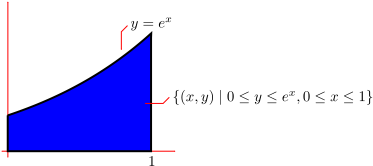
\includegraphics[width=\linewidth]{external/text/figs/etox_area.pdf}
\end{sbspanel}%
\end{sidebyside}%
\par
This area is equal to the ``definite integral''%
\begin{align*}
\text{Area} &= \int_0^1 e^x \dee{x}
\end{align*}
Do not worry about this notation or terminology just yet. We discuss  it at length below. In different applications this quantity will  have different interpretations \textemdash{} not just area. For example, if \(x\)  is time and \(e^x\) is your velocity at time \(x\), then we'll see later (in Example~\hyperref[example-eg_INTdistance]{{\xreffont\ref{example-eg_INTdistance}}}) that the specified area is the  net distance travelled between time \(0\) and time \(1\). After we finish  with the example, we'll mimic it to give a general definition of the  integral \(\int_a^b f(x) \dee{x}\).%
\begin{example}{Example}{Computing an area with vertical strips.}{example-eg_INTexparea}%
We wish to compute the area of \(\big\{\ (x,y)\ \big|\ 0\le y\le e^x\), \(0\le x\le  1\ \big\}\). We know, from our experience with \(e^x\) in differential calculus,  that the curve \(y=e^x\) is not easily written in terms of other simpler  functions, so it is very unlikely that we would be able to write the area as  a combination of simpler geometric objects such as triangles, rectangles or  circles.%
\par
So rather than trying to write down the area exactly, our strategy is to  approximate the area and then make our approximation more and more precise \footnotemark{}. We choose \footnotemark{} to approximate the area as a union of a  large number of tall thin (vertical) rectangles. As we take more and more  rectangles we get better and better approximations. Taking the limit as the  number of rectangles goes to infinity gives the exact area \footnotemark{}.%
\par
As a warm up exercise, we'll now just use four rectangles. In Example  \hyperref[example-eg_INTexpareaB]{{\xreffont\ref{example-eg_INTexpareaB}}}, below, we'll consider an arbitrary number of rectangles  and then take the limit as the number of rectangles goes to infinity. So%
\begin{itemize}[label=\textbullet]
\item{}subdivide the interval \(0\le x\le 1\) into \(4\) equal subintervals each of width \(\frac{1}{4}\), and%
\item{}subdivide the area of interest into four corresponding  vertical strips, as in the figure below.%
\end{itemize}
The area we want is exactly the sum of the areas of all four strips.%
\begin{sidebyside}{1}{0.335}{0.335}{0}%
\begin{sbspanel}{0.33}%
\includegraphics[width=\linewidth]{external/text/figs/earea1four.pdf}
\end{sbspanel}%
\end{sidebyside}%
\par
Each of these strips is almost, but not quite, a rectangle. While the bottom and  sides are fine (the sides are at right-angles to the base), the top of the strip  is not horizontal. This is where we must start to approximate. We can replace  each strip by a rectangle by just levelling off the top. But now we have to make  a choice \textemdash{} at what height do we level off the top?%
\par
Consider, for example, the leftmost strip. On this strip, \(x\) runs from \(0\) to  \(\frac{1}{4}\). As \(x\) runs from \(0\) to \(\frac{1}{4}\), the height \(y\)  runs from \(e^0\) to \(e^{\frac{1}{4}}\). It would be reasonable to choose the  height of the approximating rectangle to be somewhere between \(e^0\) and \(e^{\frac{1}{4}}\). Which%
\begin{sidebyside}{1}{0.335}{0.335}{0}%
\begin{sbspanel}{0.33}%
\includegraphics[width=\linewidth]{external/text/figs/earea3four.pdf}
\end{sbspanel}%
\end{sidebyside}%
\par
height should we choose? Well, actually it doesn't matter. When we eventually  take the limit of infinitely many approximating rectangles all of those  different choices give exactly the same final answer. We'll say more about this  later.%
\par
In this example we'll do two sample computations.%
\begin{itemize}[label=\textbullet]
\item{}For the first computation we approximate each slice by a rectangle whose height is the height of the \emph{left} hand side of the slice.%
\begin{itemize}[label=$\circ$]
\item{}On the first slice, \(x\) runs from \(0\) to \(\frac{1}{4}\),  and the height \(y\) runs from \(e^0\), on the left hand side, to  \(e^{\frac{1}{4}}\), on the right hand side.%
\item{}So we approximate the first slice by the rectangle of height \(e^0\) and width \(\frac{1}{4}\), and hence of area \(\frac{1}{4}\,e^0  =\frac{1}{4}\).%
\item{}On the second slice, \(x\) runs from \(\frac{1}{4}\) to  \(\frac{1}{2}\), and the height \(y\) runs from \(e^{\frac{1}{4}}\) and  \(e^{\frac{1}{2}}\).%
\item{}So we approximate the second slice by the rectangle of height \(e^{\frac{1}{4}}\) and width \(\frac{1}{4}\), and hence of area  \(\frac{1}{4}\,e^{\frac{1}{4}}\).%
\item{}And so on.%
\item{}All together, we approximate the area of interest by the sum of the areas of the four approximating rectangles, which is%
\begin{gather*}
\big[1+ e^{\frac{1}{4}} + e^{\frac{1}{2}} +e^{\frac{3}{4}}\big]\frac{1}{4}  =1.5124
\end{gather*}
%
\item{}This particular approximation is called the ``left Riemann sum approximation to \(\int_0^1 e^x\dee{x}\) with \(4\) subintervals''. We'll explain this  terminology later.%
\item{}This particular approximation represents the shaded area  in the figure on the left below. Note that, because \(e^x\) \emph{increases} as  \(x\) increases, this approximation is definitely smaller than the true area.%
\end{itemize}
%
\end{itemize}
%
\begin{sidebyside}{2}{0.085}{0.085}{0.17}%
\begin{sbspanel}{0.33}[center]%
\includegraphics[width=\linewidth]{external/text/figs/earea4.pdf}
\end{sbspanel}%
\begin{sbspanel}{0.33}[center]%
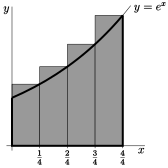
\includegraphics[width=\linewidth]{external/text/figs/earea4right.pdf}
\end{sbspanel}%
\end{sidebyside}%
\par
%
\begin{itemize}[label=\textbullet]
\item{}For the second computation we approximate each slice by a rectangle whose height is the height of the \emph{right} hand side of the slice.%
\begin{itemize}[label=$\circ$]
\item{}On the first slice, \(x\) runs from \(0\) to \(\frac{1}{4}\),  and the height \(y\) runs from \(e^0\), on the left hand side, to  \(e^{\frac{1}{4}}\), on the right hand side.%
\item{}So we approximate the first slice by the rectangle of height \(e^{\frac{1}{4}}\) and width \(\frac{1}{4}\), and hence of area  \(\frac{1}{4}\,e^{\frac{1}{4}}\).%
\item{}On the second slice, \(x\) runs from \(\frac{1}{4}\) to  \(\frac{1}{2}\), and the height \(y\) runs from \(e^{\frac{1}{4}}\) and \(e^{\frac{1}{2}}\).%
\item{}So we approximate the second slice by the rectangle of height \(e^{\frac{1}{2}}\) and width \(\frac{1}{4}\), and hence of area  \(\frac{1}{4}\,e^{\frac{1}{2}}\).%
\item{}And so on.%
\item{}All together, we approximate the area of interest by the sum of the areas of the four approximating rectangles, which is%
\begin{gather*}
\big[e^{\frac{1}{4}} + e^{\frac{1}{2}} +e^{\frac{3}{4}}+e^1\big]\frac{1}{4} =1.9420
\end{gather*}
%
\item{}This particular approximation is called the ``right Riemann sum approximation to \(\int_0^1 e^x\dee{x}\) with \(4\) subintervals''.%
\item{}This particular approximation represents the shaded area in the figure on  the right above. Note that, because \(e^x\) \emph{increases} as \(x\) increases,  this approximation is definitely larger than the true area.%
\end{itemize}
%
\end{itemize}
%
\end{example}
\footnotetext[1]{This should remind the reader of the approach taken to compute  the slope of a tangent line way way back at the start of differential calculus.\label{fn-eg_INTexparea-c-a}}%
\footnotetext[2]{Approximating the area in this way leads to a definition of integration that is called Riemann integration. This is the most  commonly used approach to integration. However we could also approximate the  area by using long thin horizontal strips. This leads to a definition of  integration that is called Lebesgue integration. We will not be covering  Lebesgue integration in these notes.\label{fn-eg_INTexparea-c-b}}%
\footnotetext[3]{If we want  to be more careful here, we should construct two approximations, one that is  always a little smaller than the desired area and one that is a little larger.  We can then take a limit using the Squeeze Theorem and arrive at the  exact area. More on this later.\label{fn-eg_INTexparea-c-c}}%
Now for the full computation that gives the exact area.%
\begin{example}{Example}{Computing an area exactly.}{example-eg_INTexpareaB}%
Recall that we wish to compute the area of%
\begin{gather*}
\big\{\ (x,y)\ \big|\ 0\le y\le  e^x,\ 0\le x\le 1\ \big\}
\end{gather*}
and that our strategy is to approximate this area by  the area of a union of a large number of very thin rectangles, and then take the limit as the number of rectangles goes to infinity. In Example~\hyperref[example-eg_INTexparea]{{\xreffont\ref{example-eg_INTexparea}}}, we used just four rectangles. Now we'll consider a  general number of rectangles, that we'll call \(n\). Then we'll take the limit  \(n\rightarrow\infty\). So%
\begin{itemize}[label=\textbullet]
\item{}pick a natural number \(n\) and%
\item{}subdivide the interval \(0\le x\le 1\) into \(n\) equal subintervals each of width \(\frac{1}{n}\), and%
\item{}subdivide the area of interest into corresponding thin strips, as in the  figure below.%
\end{itemize}
The area we want is exactly the sum of the areas of all of the thin strips.%
\begin{sidebyside}{1}{0.335}{0.335}{0}%
\begin{sbspanel}{0.33}%
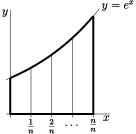
\includegraphics[width=\linewidth]{external/text/figs/earea1.pdf}
\end{sbspanel}%
\end{sidebyside}%
\par
Each of these strips is almost, but not quite, a rectangle. As in Example  \hyperref[example-eg_INTexparea]{{\xreffont\ref{example-eg_INTexparea}}}, the only problem is that the top is not horizontal. So we  approximate each strip by a rectangle, just by levelling off the top. Again, we  have to make a choice \textemdash{} at what height do we level off the top?%
\par
Consider, for example, the leftmost strip. On this strip, \(x\) runs from \(0\) to  \(\frac{1}{n}\). As \(x\) runs from \(0\) to \(\frac{1}{n}\), the height \(y\)  runs from  \(e^0\) to \(e^{\frac{1}{n}}\). It would be reasonable to choose the  height of the approximating rectangle to be somewhere between \(e^0\) and  \(e^{\frac{1}{n}}\). Which height should we choose?%
\par
Well, as we said in Example \hyperref[example-eg_INTexparea]{{\xreffont\ref{example-eg_INTexparea}}}, it doesn't matter. We shall  shortly take the limit \(n\rightarrow\infty\) and, in that limit, all of those  different choices give exactly the same final answer. We won't justify that  statement in this example, but there will be an (optional) section shortly that   provides the justification. For this example we just, arbitrarily, choose the  height of each rectangle to be the height of the graph \(y=e^x\) at the smallest  value of \(x\) in the corresponding strip \footnotemark{}. The figure on the left below shows the  approximating rectangles when \(n=4\) and the figure on the right shows the  approximating rectangles when \(n=8\).%
\begin{sidebyside}{2}{0.085}{0.085}{0.17}%
\begin{sbspanel}{0.33}[center]%
\includegraphics[width=\linewidth]{external/text/figs/earea4.pdf}
\end{sbspanel}%
\begin{sbspanel}{0.33}[center]%
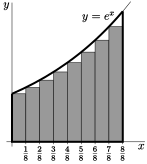
\includegraphics[width=\linewidth]{external/text/figs/earea5.pdf}
\end{sbspanel}%
\end{sidebyside}%
\par
Now we compute the approximating area when there are \(n\) strips.%
\begin{itemize}[label=\textbullet]
\item{}We approximate the leftmost strip by a rectangle of height \(e^0\). All of  the rectangles have width \(\frac{1}{n}\). So the leftmost rectangle has area  \(\frac{1}{n}e^0\).%
\item{}On strip number \(2\), \(x\) runs from \(\frac{1}{n}\) to \(\frac{2}{n}\). So the  smallest value of \(x\) on strip number \(2\) is \(\frac{1}{n}\), and we approximate  strip number \(2\) by a rectangle of height \(e^{\frac{1}{n}}\) and hence of  area \(\frac{1}{n}e^{\frac{1}{n}} \).%
\item{}And so on.%
\item{}On the last strip, \(x\) runs from \(\frac{n-1}{n}\) to \(\frac{n}{n}=1\).  So the smallest value of \(x\) on the last strip is \(\frac{n-1}{n}\), and we  approximate the last strip by a rectangle of height \(e^{\frac{(n-1)}{n}}\) and hence of area \(\frac{1}{n}e^{\frac{(n-1)}{n}} \).%
\end{itemize}
%
\par
The total area of all of the approximating rectangles is%
\begin{align*}
\text{Total approximating area} &= \frac{1}{n}e^0
+ \frac{1}{n}e^{\frac{1}{n}}
+ \frac{1}{n}e^{\frac{2}{n}}
+ \frac{1}{n}e^{\frac{3}{n}}
+ \cdots
+ \frac{1}{n}e^{\frac{(n-1)}{n}}\\
&= \frac{1}{n}\Big( 1+ e^{\frac{1}{n}} +e^{\frac{2}{n}}+e^{\frac{3}{n}}
+\cdots+ e^{\frac{(n-1)}{n}}\Big)
\end{align*}
Now the sum in the brackets might look a little intimidating because of all the  exponentials, but it actually has a pretty simple structure that can be easily  seen if we rename \(e^{\frac{1}{n}}=r\). Then%
\begin{itemize}[label=\textbullet]
\item{}the first term is 1 = \(r^0\) and%
\item{}the second term is \(e^{\frac{1}{n}}=r^1\) and%
\item{}the third term is \(e^{\frac{2}{n}}=r^2\) and%
\item{}the fourth term is \(e^{\frac{3}{n}}=r^3\) and%
\item{}and so on and%
\item{}the last term is \(e^{\frac{(n-1)}{n}}=r^{n-1}\).%
\end{itemize}
So%
\begin{align*}
\text{Total approximating area}
&= \frac{1}{n}\left( 1+ r +r^2 +\cdots+ r^{n-1}\right)
\end{align*}
The sum in brackets is known as a geometric sum and satisfies a nice simple formula:%
\begin{fact}{Equation}{Geometric sum.}{}{fact-eq_INTgeomsum}%
%
\begin{gather*}
1+ r +r^2 +\cdots+ r^{n-1} =\frac{r^n-1}{r-1} \qquad\text{provided $r\ne 1$}
\end{gather*}
%
\end{fact}
The derivation of the above formula is not too difficult. So let's  derive it in a little aside.%
\begin{aside}{Aside}{Geometric sum.}{aside-eg_INTexpareaB-l}%
Denote the sum as%
\begin{align*}
S& =1 + r + r^2 + \cdots + r^{n-1}
\end{align*}
Notice that if we multiply the whole sum by \(r\) we get back almost the same thing:%
\begin{align*}
&rS\\
&= r\left(1+ r +\cdots+ r^{n-1}\right)\\
&= r+ r^2+ r^3 +\cdots+ r^n
\end{align*}
This right hand side differs from the original sum \(S\) only in that%
\begin{itemize}[label=\textbullet]
\item{}the right hand side, which starts with ``\(r+\,\)'',  is missing the ``\(1+\,\)'' that \(S\) starts with, and%
\item{}the right hand side has an extra ``\(+r^n\,\)'' at the end that does not appear in \(S\).%
\end{itemize}
That is%
\begin{align*}
rS & = S-1+r^n\\
\intertext{Moving this around a little gives}
(r-1)S &= (r^n-1)\\
S &= \frac{r^n-1}{r-1}
\end{align*}
as required. Notice that the last step in the manipulations only works providing \(r \neq
1\) (otherwise we are dividing by zero).%
\end{aside}
Now we can go back to our area approximation armed with the above result about geometric  sums.%
\begin{align*}
\text{Total approximating area}
&= \frac{1}{n}\left( 1+ r +r^2 +\cdots+ r^{n-1}\right)\\
&= \frac{1}{n} \frac{r^n-1}{r-1} \qquad\qquad \text{remember that $r=e^{1/n}$}\\
&= \frac{1}{n} \frac{e^{n/n} - 1}{e^{1/n}-1}\\
&= \frac{1}{n} \frac{e - 1}{e^{1/n}-1}
\end{align*}
%
\par
To get the exact area \footnotemark{} all we need to  do is make the approximation better and better by taking the limit \(n\rightarrow  \infty\). The limit will look more familiar if we rename \(\frac{1}{n}\) to  \(X\). As \(n\) tends to infinity, \(X\) tends to \(0\), so%
\begin{align*}
\text{Area}&=\lim_{n\rightarrow\infty} \frac{1}{n}\ \frac{e-1}{e^{1/n}-1}\\
&=(e-1)\lim_{n\rightarrow\infty} \frac{1/n}{e^{1/n}-1}\\
&=(e-1)\lim_{X\rightarrow 0} \frac{X}{e^X-1}
&\text{(with $X=\frac{1}{n}$)}
\end{align*}
Examining this limit we see that both numerator and denominator tend to zero as \(X\to 0\),  and so we cannot evaluate this limit by computing the limits of the numerator and  denominator separately and then dividing the results. Despite this, the limit is not too  hard to evaluate; here we give two ways:%
\begin{itemize}[label=\textbullet]
\item{}Perhaps the easiest way to compute the limit is by using  l'Hôpital's rule \footnotemark{}. Since both numerator and denominator go to zero, this is a \(\frac00\) indeterminate  form. Thus%
\begin{align*}
\lim_{X\rightarrow 0} \frac{X}{e^X-1}
&=\lim_{X\rightarrow 0} \frac{\diff{}{X}X}{\diff{}{X}(e^X-1)}
=\lim_{X\rightarrow 0} \frac{1}{e^X}=1
\end{align*}
%
\item{}Another way \footnotemark{} to evaluate the same limit is to observe that it can be massaged  into the form of the limit definition of the derivative. First notice that%
\begin{align*}
\lim_{X\rightarrow 0} \frac{X}{e^X-1}
&= \left[\lim_{X\rightarrow 0} \frac{e^X-1}{X} \right]^{-1}
\end{align*}
provided this second limit exists and is nonzero \footnotemark{}. This second limit should look a little  familiar:%
\begin{align*}
\lim_{X\rightarrow 0} \frac{e^X-1}{X}
&= \lim_{X\rightarrow 0} \frac{e^X-e^0}{X-0}
\end{align*}
which is just the definition of the derivative of \(e^x\) at \(x=0\). Hence we have%
\begin{align*}
\lim_{X\rightarrow 0} \frac{X}{e^X-1}
&=\left[\lim_{X\rightarrow 0}\, \frac{e^X-e^0}{X-0} \right]^{-1}\\
&=\left[\diff{}{X}e^X\Big|_{X=0} \right]^{-1}\\
&=\left[e^X\big|_{X=0}\right]^{-1}\\
&=1
\end{align*}
%
\end{itemize}
So, after this short aside into limits, we may now conclude that%
\begin{align*}
\text{Area} &=(e-1)\lim_{X\rightarrow 0} \frac{X}{e^X-1}\\
&=e-1
\end{align*}
%
\end{example}
\footnotetext[4]{Notice that since \(e^x\) is an  increasing function, this choice of heights means that each of our rectangles is  smaller than the strip it came from.\label{fn-eg_INTexpareaB-f-e}}%
\footnotetext[5]{We haven't proved that this will give us the  exact area, but it should be clear that taking this limit will give us a lower  bound on the area. To complete things rigorously we also need an upper bound and  the squeeze theorem. We do this in the next optional subsection.\label{fn-eg_INTexpareaB-n-a}}%
\footnotetext[6]{If you do not recall L'Hôpital's rule and indeterminate forms then we recommend you skim over your differential calculus notes on the topic.\label{fn-eg_INTexpareaB-n-j-a-a}}%
\footnotetext[7]{Say if you don't recall l'Hôpital's rule and have not had time to revise it.\label{fn-eg_INTexpareaB-n-j-b-a}}%
\footnotetext[8]{To hyphenate or not to hypenate: ``non-zero'' or ``nonzero''? The authors took our lead from \href{https://gcc.gnu.org/ml/gcc/2001-10/msg00610.html}{here}\footnotemark{} and also \href{https://www.economist.com/news/books-and-arts/21723088-hyphens-can-be-tricky-they-need-not-drive-you-crazy-hysteria-over-hyphens}{here}\footnotemark{}.\label{fn-eg_INTexpareaB-n-j-b-c}}%
\footnotetext[9]{\nolinkurl{gcc.gnu.org/ml/gcc/2001-10/msg00610.html}\label{fn-eg_INTexpareaB-n-j-b-c-d}}%
\footnotetext[10]{\nolinkurl{www.economist.com/news/books-and-arts/21723088-hyphens-can-be-tricky-they-need-not-drive-you-crazy-hysteria-over-hyphens}\label{fn-eg_INTexpareaB-n-j-b-c-f}}%
\end{subsectionptx}
%
%
\typeout{************************************************}
\typeout{Subsection 1.1.2 Optional \textemdash{} A more rigorous area computation}
\typeout{************************************************}
%
\begin{subsectionptx}{Subsection}{Optional \textemdash{} A more rigorous area computation}{}{Optional \textemdash{} A more rigorous area computation}{}{}{subsection-sec_intdef-d}
In Example~\hyperref[example-eg_INTexparea]{{\xreffont\ref{example-eg_INTexparea}}} above we considered the area of the region \(\big\{\ (x,y)\ \big|\ 0\le y\le e^x\), \(0\le x\le 1\ \big\}\). We approximated that area  by  the area of a union of \(n\) thin rectangles. We then claimed that upon taking  the number of rectangles to infinity, the approximation of the area became the  exact area. However we did not justify the claim. The purpose of this optional  section is to make that calculation rigorous.%
\par
The broad set-up is the same. We divide the region up into \(n\) vertical strips,  each of width \(\frac1n\) and we then approximate those strips by rectangles.  However rather than an uncontrolled approximation, we construct two sets of  rectangles \textemdash{} one set always smaller than the original area and one always  larger. This then gives us lower and upper bounds on the area of the region.   Finally we make use of the squeeze  theorem \footnote{Recall that if we have 3 functions \(f(x), g(x), h(x)\) that satisfy \(f(x) \leq g(x) \leq  h(x)\) and we know that \(\lim_{x \to a} f(x) = \lim_{x\to a} h(x) = L\) exists and is  finite, then the squeeze theorem tells us that \(\lim_{x\to a} g(x) = L\).\label{fn-sec_intdef-d-c-d}} to establish  the result.%
\par
%
\begin{itemize}[label=\textbullet]
\item{}To find our upper and lower bounds we make use of the fact that \(e^x\) is an  increasing function. We know this because the derivative \(\diff{}{x}e^x=e^x\)  is always  positive. Consequently, the smallest and largest values of \(e^x\) on the interval  \(a\le x\le b\) are \(e^a\) and \(e^b\), respectively.%
\item{}In particular, for \(0\le x\le \frac{1}{n}\), \(e^x\) takes values only between \(e^0\) and \(e^{\frac{1}{n}}\).  As a result,  the first strip%
\begin{gather*}
\big\{\ (x,y)\ \big|\ 0\le x\le \frac{1}{n},\ 0\le y\le e^x\ \big\}
\end{gather*}
%
\begin{itemize}[label=$\circ$]
\item{}contains the rectangle of \(0\le x\le \frac{1}{n}\), \(0\le y\le e^0\)  (the lighter rectangle in the figure on the left below) and%
\item{}is contained in the rectangle \(0\le x\le \frac{1}{n}\), \(0\le y\le  e^{\frac{1}{n}}\)  (the largest rectangle in the figure on the left below).%
\end{itemize}
Hence%
\begin{gather*}
\frac{1}{n}e^{0}
\le {\rm Area}
\big\{\ (x,y)\ \big|\ 0\le x\le \frac{1}{n},\ 0\le y\le e^x\ \big\}
\le \frac{1}{n}e^{\frac{1}{n}}
\end{gather*}
%
\begin{sidebyside}{2}{0.085}{0.085}{0.17}%
\begin{sbspanel}{0.33}[center]%
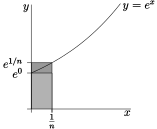
\includegraphics[width=\linewidth]{external/text/figs/earea3.pdf}
\end{sbspanel}%
\begin{sbspanel}{0.33}[center]%
\includegraphics[width=\linewidth]{external/text/figs/earea6.pdf}
\end{sbspanel}%
\end{sidebyside}%
\item{}Similarly, for the second, third, \textellipsis{}, last strips,  as in the figure on the right above,%
\begin{align*}
\frac{1}{n}e^{\frac{1}{n}}
&\le {\rm Area}\big\{\ (x,y)\ \big|\
\frac{1}{n}\le x\le \frac{2}{n},\ 0\le y\le e^x\ \big\}
\ \ \ \le \frac{1}{n}e^{\frac{2}{n}}\\
\frac{1}{n}e^{\frac{2}{n}}
&\le {\rm Area}\big\{\ (x,y)\ \big|\
\frac{2}{n}\le x\le \frac{3}{n},\ 0\le y\le e^x\ \big\}
\ \ \ \le \frac{1}{n}e^{\frac{3}{n}}\\
& \vdots\\
\frac{1}{n}e^{\frac{(n-1)}{n}}
&\le {\rm Area}\big\{\ (x,y)\ \big|\
\frac{(n-1)}{n}\le x\le \frac{n}{n},\ 0\le y\le e^x\ \big\}
\le\frac{1}{n}e^{\frac{n}{n}}
\end{align*}
%
\item{}Adding these \(n\) inequalities together gives%
\begin{align*}
&\frac{1}{n}\left(1+e^{\frac{1}{n}}+\cdots+e^{\frac{(n-1)}{n}}\right)\\
&\le {\rm Area}\big\{\ (x,y)\ \big|\ 0\le x\le 1,\ 0\le y\le e^x\ \big\}\\
&\le \frac{1}{n}\left(e^{\frac{1}{n}}+e^{\frac{2}{n}}+\cdots+
e^{\frac{n}{n}}\right)
\end{align*}
%
\item{}We can then recycle equation~\hyperref[fact-eq_INTgeomsum]{{\xreffont\ref{fact-eq_INTgeomsum}}} with \(r=e^{\frac1n}\), so  that \(r^n=\left(e^{\frac{1}{n}}\right)^n=e\). Thus we have%
\begin{gather*}
\frac{1}{n}\frac{e-1}{e^{\frac{1}{n}}-1}
\le {\rm Area}\big\{\ (x,y)\ \big|\ 0\le x\le 1,\ 0\le y\le e^x\ \big\}
\le \frac{1}{n}e^{\frac{1}{n}}\frac{e-1}{e^{\frac{1}{n}}-1}
\end{gather*}
where we have used the fact that the upper bound is a simple multiple of the  lower bound:%
\begin{align*}
\left(e^{\frac{1}{n}}+e^{\frac{2}{n}}+\cdots+
e^{\frac{n}{n}}\right)
&= e^{\frac{1}{n}}\left(1+e^{\frac{1}{n}}+\cdots
+e^{\frac{(n-1)}{n}}\right).
\end{align*}
%
\item{}We now apply the squeeze theorem to the above inequalities. In particular, the  limits of the lower and upper bounds are \(\lim_{n\rightarrow\infty}\frac{1}{n}\frac{e-1}{e^{\frac{1}{n}}-1}\) and \(\lim_{n\rightarrow\infty}\frac{1}{n}e^{\frac{1}{n}}\frac{e-1}{e^{\frac{1}{n}}-1}\), respectively. As we did near the end of Example \hyperref[example-eg_INTexpareaB]{{\xreffont\ref{example-eg_INTexpareaB}}}, we make these limits look more familiar by renaming \(\frac{1}{n}\) to \(X\). As \(n\) tends to infinity, \(X\) tends to \(0\), so the limits of the lower and upper bounds are%
\begin{align*}
\lim_{n\rightarrow\infty}\frac{1}{n}\frac{e-1}{e^{\frac{1}{n}}-1}
&=(e-1)\lim_{X=\frac{1}{n}\rightarrow 0}\frac{X}{e^X-1}
=e-1
\end{align*}
(by l'Hôpital's rule) and%
\begin{align*}
\lim_{n\rightarrow\infty}\frac{1}{n}e^{\frac{1}{n}}\frac{e-1}{e^{\frac{1}{n}}-1}
&=(e-1)\lim_{X=\frac{1}{n}\rightarrow 0}\cdot \frac{Xe^X}{e^X-1}\\
&=(e-1)\lim_{X\to 0}e^X \cdot \lim_{X=\to 0}\frac{X}{e^X-1}\\
&=(e-1) \cdot 1 \cdot 1
\end{align*}
Thus, since the exact area is trapped between the lower and upper bounds, the squeeze  theorem then implies that%
\begin{align*}
\text{Exact area} &= e-1.
\end{align*}
%
\end{itemize}
%
\end{subsectionptx}
%
%
\typeout{************************************************}
\typeout{Subsection 1.1.3 Summation notation}
\typeout{************************************************}
%
\begin{subsectionptx}{Subsection}{Summation notation}{}{Summation notation}{}{}{subsection-ssec_sum_notn}
\begin{introduction}{}%
As you can see from the above example (and the more careful rigorous computation), our  discussion of integration will involve a fair bit of work with sums of quantities. To  this end, we make a quick aside into summation notation. While one can work through the  material below without this notation, proper summation notation is well worth learning,  so we advise the reader to persevere.%
\par
Writing out the summands explicitly can become quite impractical \textemdash{} for example, say we  need the sum of the first 11 squares:%
\begin{gather*}
1 + 2^2 + 3^2 + 4^2+ 5^2 + 6^2 + 7^2 + 8^2 + 9^2 + 10^2 + 11^2
\end{gather*}
This becomes tedious. Where the pattern is clear, we will often skip the middle few  terms and instead write%
\begin{gather*}
1 + 2^2 + \cdots  + 11^2.
\end{gather*}
A far more precise way to write this is using \(\Sigma\) (capital-sigma) notation. For  example, we can write the above sum as%
\begin{gather*}
\sum_{k=1}^{11} k^2
\end{gather*}
This is read as%
\begin{quote}%
The sum from \(k\) equals 1 to 11 of \(k^2\).%
\end{quote}
More generally%
\begin{definition}{Definition}{}{definition-ssec_sum_notn-b-e}%
Let \(m\leq n\) be integers and let \(f(x)\) be a function defined on the integers. Then we write%
\begin{gather*}
\sum_{k=m}^n f(k)
\end{gather*}
to mean the sum of \(f(k)\) for \(k\) from \(m\) to \(n\):%
\begin{gather*}
f(m) + f(m+1) + f(m+2) + \cdots + f(n-1) + f(n).
\end{gather*}
Similarly we write%
\begin{gather*}
\sum_{i=m}^n a_i
\end{gather*}
to mean%
\begin{gather*}
a_m+a_{m+1}+a_{m+2}+\cdots+a_{n-1}+a_n
\end{gather*}
for some set of coefficients \(\{ a_m, \ldots, a_n \}\).%
\end{definition}
Consider the example%
\begin{gather*}
\sum_{k=3}^7 \frac{1}{k^2}=\frac{1}{3^2}+\frac{1}{4^2}+\frac{1}{5^2}+
\frac{1}{6^2}+\frac{1}{7^2}
\end{gather*}
It is important to note that the right hand side of this expression evaluates to a number \footnote{Some careful addition shows it is \(\frac{46181}{176400}\).\label{fn-ssec_sum_notn-b-f-b}}; it does not  contain ``\(k\)''.  The summation index \(k\)  is just a ``dummy'' variable and  it does not have to be called \(k\). For example%
\begin{gather*}
\sum_{k=3}^7 \frac{1}{k^2}
=\sum_{i=3}^7 \frac{1}{i^2}
=\sum_{j=3}^7 \frac{1}{j^2}
=\sum_{\ell=3}^7 \frac{1}{\ell^2}
\end{gather*}
Also the summation index has no meaning outside the sum. For example%
\begin{gather*}
k\sum_{k=3}^7 \frac{1}{k^2}
\end{gather*}
has no mathematical meaning; it is gibberish.%
\par
A sum can be represented using summation notation in many different ways. If you are unsure as to whether or not two summation notations represent the same sum, just write out the first few terms and the last  couple of terms. For example,%
\begin{align*}
\sum_{m=3}^{15} \frac{1}{m^2}
&=\overbrace{\frac{1}{3^2}}^{m=3}
+\overbrace{\frac{1}{4^2}}^{m=4}
+\overbrace{\frac{1}{5^2}}^{m=5}
+\cdots
+\overbrace{\frac{1}{14^2}}^{m=14}
+\overbrace{\frac{1}{15^2}}^{m=15}\\
\sum_{m=4}^{16} \frac{1}{(m-1)^2}
&=\overbrace{\frac{1}{3^2}}^{m=4}
+\overbrace{\frac{1}{4^2}}^{m=5}
+\overbrace{\frac{1}{5^2}}^{m=6}
+\cdots
+\overbrace{\frac{1}{14^2}}^{m=15}
+\overbrace{\frac{1}{15^2}}^{m=16}
\end{align*}
are equal.%
\par
Here is a theorem that gives a few rules for manipulating summation notation.%
\begin{theorem}{Theorem}{Arithmetic of Summation Notation.}{}{theorem-thm_INTsummationArith}%
Let \(n\ge m\) be integers. Then for all real numbers \(c\) and \(a_i,b_i\), \(m\le i\le n\).%
\begin{enumerate}[label=\alph*]
\item{}\(\displaystyle \sum\limits_{i=m}^nca_i = c\bigg(\sum\limits_{i=m}^na_i\bigg)\)%
\item{}\(\displaystyle \sum\limits_{i=m}^n(a_i+b_i) = \bigg(\sum\limits_{i=m}^na_i\bigg) + \bigg(\sum\limits_{i=m}^nb_i\bigg)\)%
\item{}\(\displaystyle \sum\limits_{i=m}^n(a_i-b_i) = \bigg(\sum\limits_{i=m}^na_i\bigg)  - \bigg(\sum\limits_{i=m}^nb_i\bigg)\)%
\end{enumerate}
%
\end{theorem}
\begin{proof}{Proof}{}{proof-ssec_sum_notn-b-j}
We can prove this theorem by just writing out both sides of each equation, and observing that they are equal, by the usual laws of arithmetic \footnote{Since all  the sums are finite, this isn't too hard. More care must be taken when the sums involve  an infinite number of terms. We will examine this in Chapter~\mono{[cross-reference to target(s) \textquotedbl{}chap\_seq\_ser\textquotedbl{} missing or not unique]}.\label{fn-ssec_sum_notn-b-j-a-a}}. For example, for the first equation, the left and right hand sides are%
\begin{gather*}
\sum_{i=m}^nca_i = ca_m+ca_{m+1}+\cdots+ca_n\\
\quad\text{and}\quad
c\bigg(\sum\limits_{i=m}^na_i\bigg) = c(a_m+a_{m+1}+\cdots+a_n)
\end{gather*}
They are equal by the usual distributive law. The ``distributive law'' is the fancy name for \(c(a+b)=ca+cb\).%
\end{proof}
Not many sums can be computed exactly \footnote{Of course, any finite sum can be computed  exactly \textemdash{} just sum together the terms. What we mean by ``computed exactly'' in this  context, is that we can rewrite the sum as a simple, and easily  evaluated, formula involving the terminals of the sum. For example \(\sum_{k=m}^n r^k = \frac{r^{n+1}-r^m}{r-1}\) provided \(r\neq1\). No matter what finite integers we choose for \(m\) and \(n\), we can quickly compute the sum  in just a few arithmetic operations. On the other hand, the sums, \(\sum_{k=m}^n \frac{1}{k}\) and \(\sum_{k=m}^n \frac{1}{k^2}\), cannot be expressed in such clean formulas (though you can rewrite them quite cleanly  using integrals). To explain more clearly we would need to go into a more detailed and  careful discussion that is beyond the scope of this course.\label{fn-ssec_sum_notn-b-k-a}}. Here are some that can. The  first few are used a lot.%
\begin{theorem}{Theorem}{}{}{theorem-thm_INTspecialSums}%
%
\begin{enumerate}[label=\alph*]
\item{}\(\sum\limits_{i=0}^n ar^i = a\frac{1-r^{n+1}}{1-r}\), for all real numbers \(a\) and \(r\ne 1\) and all integers \(n\ge 0\).%
\item{}\(\sum\limits_{i=1}^n 1 = n\), for all integers \(n\ge 1\).%
\item{}\(\sum\limits_{i=1}^n i = \frac{1}{2}n(n+1)\), for all integers \(n\ge 1\).%
\item{}\(\sum\limits_{i=1}^n i^2 = \frac{1}{6}n(n+1)(2n+1)\), for all integers \(n\ge 1\).%
\item{}\(\sum\limits_{i=1}^n i^3 = \Big[\frac{1}{2}n(n+1)\Big]^2\), for all integers \(n\ge 1\).%
\end{enumerate}
%
\end{theorem}
\end{introduction}%
%
%
\typeout{************************************************}
\typeout{Subsubsection 1.1.3.1 Proof of Theorem {\xreffont\ref*{theorem-thm_INTspecialSums}} (Optional)}
\typeout{************************************************}
%
\begin{subsubsectionptx}{Subsubsection}{Proof of Theorem {\xreffont\ref*{theorem-thm_INTspecialSums}} (Optional)}{}{Proof of Theorem {\xreffont\ref*{theorem-thm_INTspecialSums}} (Optional)}{}{}{subsubsection-ssec_sum_notn-c}
\begin{proof}{Proof}{}{proof-ssec_sum_notn-c-b}
%
\begin{enumerate}[label=\alph*]
\item{}The first sum is%
\begin{gather*}
\sum_{i=0}^n ar^i =ar^0 + ar^1 + ar^2 + \cdots + ar^n
\end{gather*}
which is just the left hand side of equation~\hyperref[fact-eq_INTgeomsum]{{\xreffont\ref{fact-eq_INTgeomsum}}}, with \(n\)  replaced by \(n+1\) and then multiplied by \(a\).%
\item{}The second sum is just \(n\) copies of \(1\) added together, so of course the sum is \(n\).%
\item{}The third and fourth sums are discussed in the appendix of the CLP-1 text. In that discussion certain ``tricks'' are used to compute the  sums with only simple arithmetic. Those tricks do not easily generalise to the fifth sum.%
\item{}Instead of repeating that appendix, we'll derive the third sum  using a trick that  generalises to the fourth and fifth sums (and also to higher powers). The trick uses the generating function \footnote{Generating functions are frequently used in mathematics to  analyse sequences and series, but are beyond the scope of the course. The interested  reader should take a look at ``Generatingfunctionology'' by Herb  Wilf. It is an excellent book and is also free to download.\label{fn-ssec_sum_notn-c-b-a-a-d-a-a}} \(S(x)\):%
\begin{fact}{Equation}{Finite geometric sum.}{}{fact-eq_INTpowergenfnl}%
%
\begin{align*}
S(x) = 1+x+x^2+\cdots+x^n &= \frac{x^{n+1}-1}{x-1}
\end{align*}
%
\end{fact}
Notice that this is just the geometric sum given by equation~\hyperref[fact-eq_INTgeomsum]{{\xreffont\ref{fact-eq_INTgeomsum}}} with \(n\)  replaced by \(n+1\).%
\par
Now, consider the limit%
\begin{align*}
\lim_{x\to 1} S(x) &= \lim_{x\to 1} \left(1+x+x^2+\cdots+x^n\right) = n+1 \qquad \text{but also}\\
&= \lim_{x\to 1} \frac{x^{n+1}-1}{x-1} \qquad\qquad\qquad \text{now use l'Hôpital's rule}\\
&= \lim_{x\to 1} \frac{(n+1)x^n}{1} = n+1.
\end{align*}
This is not so hard (or useful). But now consider the derivative of \(S(x)\):%
\begin{align*}
S'(x) &= 1 +2x + 3x^2 + \cdots + n x^{n-1}\\
&= \diff{}{x} \left[\frac{x^{n+1}-1}{x-1}\right] \qquad\qquad\qquad\qquad  \text{use the quotient rule}\\
&= \frac{(x-1)\cdot (n+1)x^n - (x^{n+1}-1)\cdot 1}{(x-1)^2} \qquad  \text{now clean it up}\\
&= \frac{nx^{n+1}-(n+1)x^n+1}{(x-1)^2}.
\end{align*}
Hence if we take the limit of the above expression as \(x\to 1\) we recover%
\begin{align*}
\lim_{x\to 1} S'(x) &= 1 +2 +3+\cdots+n\\
&=\lim_{x\to 1} \frac{nx^{n+1}-(n+1)x^n+1}{(x-1)^2} \qquad\qquad \text{now use l'Hôpital's rule}\\
&=\lim_{x\to 1} \frac{n(n+1)x^{n}-n(n+1)x^{n-1}}{2(x-1)} \qquad \text{l'Hôpital's rule again}\\
&=\lim_{x\to 1} \frac{n^2(n+1)x^{n-1}-n(n+1)(n-1)x^{n-2}}{2}\\
&= \frac{n^2(n+1) - n(n-1)(n+1)}{2} = \frac{n(n+1)}{2}
\end{align*}
as required. This computation can be done without l'Hôpital's rule, but the manipulations required are a fair bit messier.%
\item{}The derivation of the fourth and fifth sums is similar to, but  even more tedious than, that of the third sum. One takes two or three  derivatives of the generating functional.%
\end{enumerate}
%
\end{proof}
\end{subsubsectionptx}
\end{subsectionptx}
%
%
\typeout{************************************************}
\typeout{Subsection 1.1.4 The Definition of the Definite Integral}
\typeout{************************************************}
%
\begin{subsectionptx}{Subsection}{The Definition of the Definite Integral}{}{The Definition of the Definite Integral}{}{}{subsection-sec_defInt}
In this section we give a definition of the definite integral \(\ds \int_a^b f(x)\dee{x}\)  generalising the machinery we used in Example~\hyperref[example-eg_INTexparea]{{\xreffont\ref{example-eg_INTexparea}}}. But first some  terminology and a couple of remarks to better motivate the definition.%
\begin{definition}{Definition}{}{definition-sec_defInt-c}%
The symbol \(\ds \int_a^b f(x)\dee{x}\) is read ``the definite integral of the function  \(f(x)\) from \(a\) to \(b\)''. The function \(f(x)\) is called the integrand of \(\int_a^b  f(x)\dee{x}\) and \(a\) and \(b\) are called \footnotemark{} the limits of integration. The interval \(a\le x \le b\) is called the interval of integration and is also called the domain of integration.%
\end{definition}
\footnotetext[16]{\(a\) and \(b\) are also called the bounds of integration.\label{fn-sec_defInt-c-a-a-g}}%
Before we explain more precisely what the definite integral actually is, a few remarks  (actually \textemdash{} a few interpretations) are in order.%
\begin{itemize}[label=\textbullet]
\item{}If \(f(x)\ge 0\) and \(a\le b\), one interpretation of the symbol \(\ds \int_a^b f(x)\dee{x}\) is ``the area of the region \(\big\{\ (x,y)\ \big|\ a\le x\le b,\   0\le y\le f(x)\ \big\}\)''.%
\begin{sidebyside}{1}{0.17}{0.17}{0}%
\begin{sbspanel}{0.66}%
\includegraphics[width=\linewidth]{external/text/figs/areaSqrt.pdf}
\end{sbspanel}%
\end{sidebyside}%
\par
In this way we can rewrite the area in Example~\hyperref[example-eg_INTexparea]{{\xreffont\ref{example-eg_INTexparea}}} as the definite  integral \(\int_0^1 e^x \dee{x}\).%
\item{}This interpretation breaks down when either \(a \gt b\) or \(f(x)\) is not always positive,  but it can be repaired by considering ``signed areas''.%
\item{}If \(a\le b\), but \(f(x)\) is not always positive, one interpretation of \(\int_a^b  f(x)\dee{x}\) is ``the signed area between \(y=f(x)\) and the \(x\)-axis for \(a\le x\le b\)''.  For ``signed area'' (which is also called the ``net area''), areas above the \(x\)-axis  count as positive while areas below the \(x\)-axis count as negative. In the example  below,  we have the graph of the function%
\begin{align*}
f(x)=\begin{cases}
-1 & \text{if }1\le x\le 2\\
2  & \text{if }2 \lt  x\le 4 \\
0 & \text{otherwise}
\end{cases}
\end{align*}
The \(2\times 2\) shaded square above the \(x\)-axis has signed area \(+2\times 2=+4\). The \(1\times 1\) shaded square below the \(x\)-axis has signed area \(-1\times 1=-1\). So, for this \(f(x)\),%
\begin{gather*}
\int_0^5 f(x)\dee{x} = +4-1=3
\end{gather*}
%
\begin{sidebyside}{1}{0.17}{0.17}{0}%
\begin{sbspanel}{0.66}%
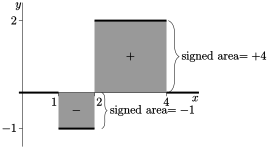
\includegraphics[width=\linewidth]{external/text/figs/signedArea.pdf}
\end{sbspanel}%
\end{sidebyside}%
\item{}We'll come back to the case \(b \lt a\) later.%
\end{itemize}
We're now ready to define \(\int_a^b f(x)\dee{x}\). The definition is a little involved,  but essentially mimics what we did in Example~\hyperref[example-eg_INTexparea]{{\xreffont\ref{example-eg_INTexparea}}} (which is why we did  the example before the definition). The main differences are that we replace the function  \(e^x\) by a generic function \(f(x)\) and we replace the interval from \(0\) to \(1\) by the  generic interval \footnote{We'll eventually allow \(a\) and \(b\) to be any two real numbers,  not even requiring \(a \lt b\). But it is easier to start off assuming \(a \lt b\), and that's what  we'll do.\label{fn-sec_defInt-d-j}} from \(a\) to \(b\).%
\begin{itemize}[label=\textbullet]
\item{}We start by selecting any natural number \(n\) and subdividing the interval from \(a\) to \(b\) into \(n\) equal subintervals. Each subinterval has width \(\frac{b-a}{n}\).%
\item{}Just as was the case in Example~\hyperref[example-eg_INTexparea]{{\xreffont\ref{example-eg_INTexparea}}} we will eventually take the  limit as \(n\to\infty\), which squeezes the width of each subinterval down to zero.%
\item{}For each integer \(0\le i\le n\), define \(x_i = a + i \cdot\frac{b-a}{n}\). Note that  this means that \(x_0=a\) and \(x_n = b\). It is worth keeping in mind that these numbers  \(x_i\) do depend on \(n\) even though our choice of notation hides this dependence.%
\item{}Subinterval number \(i\) is \(x_{i-1} \leq x \leq  x_i\). In particular, on the first subinterval, \(x\) runs from \(x_0=a\) to \(x_1=a+\frac{b-a}{n}\). On the second subinterval, \(x\) runs from \(x_1\) to \(x_2=a+2\frac{b-a}{n}\).%
\begin{sidebyside}{1}{0.17}{0.17}{0}%
\begin{sbspanel}{0.66}%
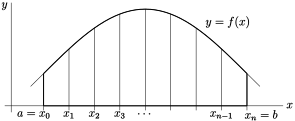
\includegraphics[width=\linewidth]{external/text/figs/intDecompE.pdf}
\end{sbspanel}%
\end{sidebyside}%
\item{}On each subinterval we now pick \(x_{i,n}^*\) between \(x_{i-1}\) and \(x_i\). We then  approximate \(f(x)\) on the \(i^\mathrm{th}\) subinterval by the constant function  \(y=f(x_{i,n}^*)\). We include \(n\) in the subscript to remind ourselves that these numbers  depend on \(n\).%
\par
Geometrically, we're approximating the region%
\begin{gather*}
\big\{\ (x,y)\ \big|\
\text{$x$ is between $x_{i-1}$ and $x_i$, and $y$ is between $0$ and $f(x)$} \ \big\}
\end{gather*}
by the rectangle%
\begin{gather*}
\big\{\ (x,y)\ \big|\
\text{$x$ is between $x_{i-1}$ and $x_i$, and $y$ is between $0$ and $f(x_{i,n}^*)$} \ \big\}
\end{gather*}
%
\begin{sidebyside}{1}{0.335}{0.335}{0}%
\begin{sbspanel}{0.33}%
\includegraphics[width=\linewidth]{external/text/figs/rect_approx_adr1.pdf}
\end{sbspanel}%
\end{sidebyside}%
\par
In Example~\hyperref[example-eg_INTexparea]{{\xreffont\ref{example-eg_INTexparea}}} we chose \(x_{i,n}^* = x_{i-1}\) and so we  approximated the function \(e^x\) on each subinterval by the value it took at the leftmost  point in that subinterval.%
\item{}So, when there are \(n\) subintervals our approximation to the signed area between the curve \(y=f(x)\) and the \(x\)-axis, with \(x\) running from \(a\) to \(b\), is%
\begin{gather*}
\sum_{i=1}^n f(x_{i,n}^*)\cdot \frac{b-a}{n}
\end{gather*}
We interpret this as the signed area since the summands \(f(x_{i,n}^*)\cdot\frac{b-a}{n}\)  need not be positive.%
\item{}Finally we define the definite integral by taking the limit of this sum as  \(n\rightarrow\infty\).%
\end{itemize}
Oof! This is quite an involved process, but we can now write down the definition we need.%
\begin{definition}{Definition}{}{definition-def_INTintegral}%
Let \(a\) and \(b\) be two real numbers and let \(f(x)\) be a function that is defined for all \(x\) between \(a\) and \(b\). Then we define%
\begin{gather*}
\int_a^b f(x)\dee{x} =\lim_{n\rightarrow\infty}\sum_{i=1}^n f(x_{i,n}^*)\cdot\frac{b-a}{n}
\end{gather*}
when the limit exists and takes the same value for all choices of  the \(x_{i,n}^*\)'s. In this case, we say that \(f\) is integrable on the  interval from \(a\) to \(b\).%
\end{definition}
Of course, it is not immediately obvious when this limit should exist. Thankfully it is  easier for a function to be ``integrable'' than it is for it to be ``differentiable''.%
\begin{theorem}{Theorem}{}{}{theorem-thm_integrable}%
Let \(f(x)\) be a function on the interval \([a,b]\). If%
\begin{itemize}[label=\textbullet]
\item{}\(f(x)\) is continuous on \([a,b]\), or%
\item{}\(f(x)\) has a finite number of jump discontinuities on \([a,b]\) (and is otherwise  continuous)%
\end{itemize}
then \(f(x)\) is integrable on \([a,b]\).%
\end{theorem}
We will not justify this theorem. But a slightly weaker statement is proved in (the optional) Section~\hyperref[subsection-ssec_careful_defn]{{\xreffont\ref{subsection-ssec_careful_defn}}}. Of course this does not tell us how to  actually evaluate any definite integrals \textemdash{} but we will get to that in time.%
\par
Some comments:%
\begin{itemize}[label=\textbullet]
\item{}Note that, in Definition \hyperref[definition-def_INTintegral]{{\xreffont\ref{definition-def_INTintegral}}}, we allow \(a\) and \(b\) to be any two real numbers. We do not require that \(a \lt b\). That is, even when \(a \gt b\), the symbol \(\int_a^b f(x)\dee{x}\) is still defined by the formula of Definition \hyperref[definition-def_INTintegral]{{\xreffont\ref{definition-def_INTintegral}}}. We'll get an interpretation for \(\int_a^b f(x)\dee{x}\), when \(a \gt b\), later.%
\item{}It is important to note that the definite integral \(\int_a^b f(x)\dee{x}\)  represents a number, not a function of \(x\). The integration variable \(x\)  is another ``dummy'' variable, just like the summation index \(i\) in  \(\sum_{i=m}^n a_i\) (see Section~\hyperref[subsection-ssec_sum_notn]{{\xreffont\ref{subsection-ssec_sum_notn}}}). The integration variable does not  have to be called \(x\). For example%
\begin{gather*}
\int_a^b f(x)\dee{x} = \int_a^b f(t)\dee{t} = \int_a^b f(u)\dee{u}
\end{gather*}
Just as with summation variables, the integration variable \(x\) has no meaning outside of \(f(x)\dee{x}\). For example%
\begin{gather*}
x\int_0^1 e^x\dee{x}\qquad\text{and}\qquad  \int_0^x e^x\dee{x}
\end{gather*}
are both gibberish.%
\end{itemize}
%
\par
The sum inside definition~\hyperref[definition-def_INTintegral]{{\xreffont\ref{definition-def_INTintegral}}} is named after Bernhard Riemann \footnote{Bernhard Riemann was a 19th century German mathematician who  made  extremely important contributions to many different areas of mathematics \textemdash{} far  too  many to list here. Arguably two of the most important (after Riemann sums) are  now  called Riemann surfaces and the Riemann hypothesis (he didn't name them after  himself).\label{fn-sec_defInt-j-c}} who made the first rigorous definition of the definite integral and so placed  integral  calculus on rigorous footings.%
\begin{definition}{Definition}{}{definition-def_INTthreeRiemannSums}%
The sum \(\ds \) inside definition~\hyperref[definition-def_INTintegral]{{\xreffont\ref{definition-def_INTintegral}}}%
\begin{gather*}
\sum_{i=1}^n f(x_{i,n}^*)\,\frac{b-a}{n}
\end{gather*}
is called a Riemann sum. It is also often written as%
\begin{gather*}
\sum_{i=1}^n f(x_i^*)\,\De x
\end{gather*}
where \(\De x = \frac{b-a}{n}\).%
\begin{itemize}[label=\textbullet]
\item{}If we choose each \(x_{i,n}^* = x_{i-1}=a+(i-1)\frac{b-a}{n}\) to be the  left hand end point of the \(i^{\rm th}\) interval, \([x_{i-1},x_i]\),  we get the approximation%
\begin{gather*}
\sum_{i=1}^n f\left(a+(i-1)\frac{b-a}{n}\right)\,\frac{b-a}{n}
\end{gather*}
which is called the ``left Riemann sum approximation to \(\int_a^b f(x)\dee{x}\) with \(n\) subintervals''. This is the approximation used  in  Example~\hyperref[example-eg_INTexparea]{{\xreffont\ref{example-eg_INTexparea}}}.%
\item{}In the same way, if we choose \(x_{i,n}^* = x_{i}=a+i\frac{b-a}{n}\) we  obtain the approximation%
\begin{gather*}
\sum_{i=1}^n f\left(a+i\frac{b-a}{n}\right)\,\frac{b-a}{n}
\end{gather*}
which is called the ``right Riemann sum approximation to \(\int_a^b f(x)\dee{x}\) with \(n\) subintervals''. The word ``right'' signifies  that, on each  subinterval \([x_{i-1},x_i]\) we approximate \(f\) by its value at the right-hand  end-point,  \(x_i=a+i\frac{b-a}{n}\), of the subinterval.%
\item{}A third commonly used approximation is%
\begin{gather*}
\sum_{i=1}^n f\left(a+(i-\frac12)\frac{b-a}{n}\right)\,\frac{b-a}{n}
\end{gather*}
which is called the ``midpoint Riemann sum approximation to \(\int_a^b f(x)\dee{x}\) with \(n\) subintervals''. The word ``midpoint'' signifies that, on each subinterval \([x_{i-1},x_i]\) we approximate \(f\) by its value at the midpoint, \(\frac{x_{i-1}+x_i}{2} =a+(i-\frac{1}{2})\frac{b-a}{n}\), of the subinterval.%
\end{itemize}
%
\end{definition}
In order to compute a definite integral using Riemann sums we need to be able to  compute  the limit of the sum as the number of summands goes to infinity. This approach  is not  always feasible and we will soon arrive at other means of computing definite  integrals  based on antiderivatives. However, Riemann sums also provide us with a good  means of  approximating definite integrals \textemdash{} if we take \(n\) to be a large, but finite,  integer,  then the corresponding Riemann sum can be a good approximation of the definite  integral.  Under certain circumstances this can be strengthened to give rigorous bounds on  the integral. Let us revisit Example~\hyperref[example-eg_INTexparea]{{\xreffont\ref{example-eg_INTexparea}}}.%
\begin{example}{Example}{Upper and lower bounds on area.}{example-sec_defInt-m}%
Let's say we are again interested in the integral \(\int_0^1 e^x\dee{x}\). We can  follow  the same procedure as we used previously to construct Riemann sum  approximations. However  since the integrand \(f(x)=e^x\) is an increasing function, we can make our  approximations  into upper and lower bounds without much extra work.%
\par
More precisely, we approximate \(f(x)\) on each subinterval \(x_{i-1}\le x\le x_i\)%
\begin{itemize}[label=\textbullet]
\item{}by its smallest value on the subinterval, namely \(f(x_{i-1})\), when  we compute the left Riemann sum approximation and%
\item{}by its largest value on the subinterval, namely \(f(x_i)\), when we  compute the right Riemann sum approximation.%
\end{itemize}
This is illustrated in the two figures below. The shaded region in the left hand figure is the left Riemann sum approximation and the  shaded region in the right hand figure is the right Riemann sum approximation.%
\begin{sidebyside}{2}{0.085}{0.085}{0.17}%
\begin{sbspanel}{0.33}[center]%
\includegraphics[width=\linewidth]{external/text/figs/earea7.pdf}
\end{sbspanel}%
\begin{sbspanel}{0.33}[center]%
\includegraphics[width=\linewidth]{external/text/figs/earea8.pdf}
\end{sbspanel}%
\end{sidebyside}%
\par
We can see that exactly because \(f(x)\) is increasing, the left Riemann sum  describes an area smaller than the definite integral while the right Riemann sum  gives an  area larger \footnotemark{} than the integral.%
\par
When we approximate the integral \(\int_0^1 e^x\dee{x}\) using \(n\) subintervals, then, on interval number~\(i\),%
\begin{itemize}[label=\textbullet]
\item{}\(x\) runs from \(\frac{i-1}{n}\) to \(\frac{i}{n}\) and%
\item{}\(y=e^x\) runs from \(e^{\frac{(i-1)}{n}}\), when \(x\) is at the left hand end point of the interval, to \(e^{\frac{i}{n}}\), when \(x\) is at the right hand end point of the interval.%
\end{itemize}
Consequently, the left Riemann sum approximation to \(\int_0^1 e^x\dee{x}\) is \(\sum_{i=1}^n e^{\frac{(i-1)}{n}}\,\frac{1}{n}\) and the  right Riemann sum approximation is  \(\sum_{i=1}^n e^{\frac{i}{n}}\cdot\frac{1}{n}\). So%
\begin{gather*}
\sum_{i=1}^n e^{\frac{(i-1)}{n}}\,\frac{1}{n}
\ \le\ \int_0^1 e^x\dee{x}\ \le\
\sum_{i=1}^n e^{\frac{i}{n}}\cdot\frac{1}{n}
\end{gather*}
Thus  \(L_n=\sum_{i=1}^n e^{\frac{(i-1)}{n}}\,\frac{1}{n}\), which for any \(n\) can be evaluated by computer, is a lower bound on the exact value of   \(\int_0^1 e^x\dee{x}\) and  \(R_n=\sum_{i=1}^n e^{\frac{i}{n}}\,\frac{1}{n}\), which for any \(n\) can also be evaluated by computer, is an upper bound on the exact value  of  \(\int_0^1 e^x\dee{x}\). For example, when \(n=1000\), \(L_n= 1.7174\) and  \(R_n=1.7191\) (both to four decimal places) so that, again to four  decimal places,%
\begin{gather*}
1.7174 \le \int_0^1 e^x\dee{x} \le 1.7191
\end{gather*}
Recall that the exact value is \(e-1 = 1.718281828\dots\).%
\end{example}
\footnotetext[19]{When a function is decreasing the situation is reversed \textemdash{}  the  left Riemann sum is always larger than the integral while the right Riemann sum  is  smaller than the integral. For more general functions that both increase and  decrease it  is perhaps easiest to study each increasing (or decreasing) interval  separately.\label{fn-sec_defInt-m-e-b}}%
\end{subsectionptx}
%
%
\typeout{************************************************}
\typeout{Subsection 1.1.5 Using Known Areas to Evaluate Integrals}
\typeout{************************************************}
%
\begin{subsectionptx}{Subsection}{Using Known Areas to Evaluate Integrals}{}{Using Known Areas to Evaluate Integrals}{}{}{subsection-ssec_knownareas}
One of the main aims of this course is to build up general machinery for  computing  definite integrals (as well as interpreting and applying them). We shall start  on this  soon, but not quite yet. We have already seen one concrete, if laborious, method  for  computing definite integrals \textemdash{} taking limits of Riemann sums as we did in  Example~\hyperref[example-eg_INTexparea]{{\xreffont\ref{example-eg_INTexparea}}}. A second method, which will work for some special  integrands, works by interpreting the definite integral as ``signed area''.  This  approach will work nicely when the area under the curve decomposes into simple  geometric  shapes like triangles, rectangles and circles. Here are some examples of this  second method.%
\begin{example}{Example}{A very simple integral and a very simple area.}{example-ssec_knownareas-c}%
The integral \(\int_a^b 1\dee{x}\) (which is also written as just \(\int_a^b\dee{x}\)) is  the  area of the shaded rectangle (of width \(b-a\) and height \(1\)) in the figure on  the right below. So%
\begin{sidebyside}{2}{0.0675}{0.0675}{0.135}%
\begin{sbspanel}{0.33}[center]%
\(\int_a^b\dee{x} = (b-a)\times (1)=b-a\)%
\end{sbspanel}%
\begin{sbspanel}{0.4}[center]%
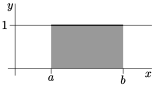
\includegraphics[width=\linewidth]{external/text/figs/areaRect.pdf}
\end{sbspanel}%
\end{sidebyside}%
\end{example}
\begin{example}{Example}{Another simple integral.}{example-eg_INTtriangle}%
Let \(b \gt 0\). The integral \(\int_0^b x\dee{x}\)  is the area of the shaded triangle (of base \(b\) and of height \(b\)) in the figure on the right below. So%
\begin{sidebyside}{2}{0.085}{0.085}{0.17}%
\begin{sbspanel}{0.33}[center]%
\(\int_0^b x\dee{x} = \frac{1}{2}b\times b=\frac{b^2}{2}\)%
\end{sbspanel}%
\begin{sbspanel}{0.33}[center]%
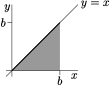
\includegraphics[width=\linewidth]{external/text/figs/areaX.pdf}
\end{sbspanel}%
\end{sidebyside}%
\par
The integral \(\int_{-b}^0 x\dee{x}\)  is the signed area of the shaded triangle (again of base \(b\) and of height \(b\)) in the figure on  the right below. So%
\begin{sidebyside}{2}{0.085}{0.085}{0.17}%
\begin{sbspanel}{0.33}[center]%
\(\int_{-b}^0 x\dee{x} = -\frac{b^2}{2} \)%
\end{sbspanel}%
\begin{sbspanel}{0.33}[center]%
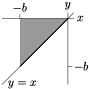
\includegraphics[width=\linewidth]{external/text/figs/areaMX.pdf}
\end{sbspanel}%
\end{sidebyside}%
\end{example}
Notice that it is very easy to extend this example to the integral \(\int_0^b  c x\dee{x}\) for any real numbers \(b,c \gt 0\) and find%
\begin{align*}
\int_0^b c x\dee{x} &= \frac{c}{2} b^2.
\end{align*}
%
\begin{example}{Example}{Evaluating \(\int_{-1}^1 \left(1-|x|\right)\dee{x}\).}{example-eg_INTtriangleB}%
In this example, we shall evaluate \(\int_{-1}^1 \left(1-|x|\right)\dee{x}\). Recall that%
\begin{align*}
|x|=\begin{cases} -x &\text{if $x\le 0$} \\
x &\text{if $x\ge 0$}
\end{cases}
\end{align*}
so that%
\begin{align*}
1-|x|=\begin{cases} 1+x &\text{if $x\le 0$}\\
1-x &\text{if $x\ge 0$}
\end{cases}
\end{align*}
To picture the geometric figure whose area the integral represents observe that%
\begin{itemize}[label=\textbullet]
\item{}at the left hand end of the domain of integration \(x=-1\) and  the integrand \(1-|x|=1-|-1|=1-1=0\) and%
\item{}as \(x\) increases from \(-1\) towards \(0\), the integrand \(1-|x|=1+x\) increases linearly, until%
\item{}when \(x\) hits \(0\) the integrand hits  \(1-|x|=1-|0|=1\) and then%
\item{}as \(x\) increases from \(0\), the integrand \(1-|x|=1-x\) decreases linearly, until%
\item{}when \(x\) hits \(+1\), the right hand end of the domain of integration, the  integrand hits   \(1-|x|=1-|1|=0\).%
\end{itemize}
So the integral \(\int_{-1}^1 \left(1-|x|\right)\dee{x}\)  is the area of the shaded triangle (of base \(2\) and of height \(1\)) in the figure on  the right below and%
\begin{sidebyside}{2}{0.085}{0.085}{0.17}%
\begin{sbspanel}{0.33}[center]%
\(\int_{-1}^1 \left(1-|x|\right)\dee{x} = \frac{1}{2}\times 2\times 1 =
1\)%
\end{sbspanel}%
\begin{sbspanel}{0.33}[center]%
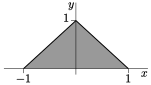
\includegraphics[width=\linewidth]{external/text/figs/areaAbs.pdf}
\end{sbspanel}%
\end{sidebyside}%
\end{example}
\begin{example}{Example}{Evaluating \(\int_0^1 \sqrt{1-x^2}\dee{x}\).}{example-eg_quarter_circle}%
The integral \(\int_0^1 \sqrt{1-x^2}\dee{x}\)  has integrand \(f(x)=\sqrt{1-x^2}\). So it represents the area under \(y=\sqrt{1-x^2}\) with \(x\) running from \(0\) to \(1\). But we may rewrite%
\begin{align*}
y&=\sqrt{1-x^2} &\text{as}&& x^2+y^2&= 1, y\geq 0
\end{align*}
But this is the (implicit) equation for a circle \textemdash{} the extra condition that  \(y\geq0\)  makes it the equation for the semi-circle centred at the origin with radius 1  lying on  and above the \(x\)-axis. Thus the integral represents the area of the quarter  circle of  radius \(1\), as shown in the figure on the right below. So%
\begin{sidebyside}{2}{0.105}{0.105}{0.21}%
\begin{sbspanel}{0.33}[center]%
\(\int_0^1 \sqrt{1-x^2}\dee{x} = \frac{1}{4}\pi(1)^2 = \frac{\pi}{4}\)%
\end{sbspanel}%
\begin{sbspanel}{0.25}[center]%
\includegraphics[width=\linewidth]{external/text/figs/areaCirc.pdf}
\end{sbspanel}%
\end{sidebyside}%
\end{example}
This next one is a little trickier and relies on us knowing the symmetries of the  sine  function.%
\begin{example}{Example}{Integrating sine.}{example-ssec_knownareas-i}%
The integral \(\int_{-\pi}^\pi \sin x\dee{x}\)  is the signed area of the shaded region in the figure on the right below. It naturally splits into  two  regions, one on either side of the \(y\)-axis. We don't know the formula for the  area of  either of these regions (yet), however the two regions are very nearly the same.  In  fact, the part of the shaded region below the \(x\)-axis is exactly the reflection, in the \(x\)-axis, of the part of the shaded region above the \(x\)-axis. So the signed area of part of the shaded region below the \(x\)-axis is the negative of the signed area of part of the shaded region above the \(x\)-axis and%
\begin{sidebyside}{2}{0.0675}{0.0675}{0.135}%
\begin{sbspanel}{0.33}[center]%
\(\int_{-\pi}^\pi \sin x\dee{x} = 0\)%
\end{sbspanel}%
\begin{sbspanel}{0.4}[center]%
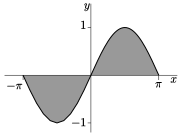
\includegraphics[width=\linewidth]{external/text/figs/areaSin.pdf}
\end{sbspanel}%
\end{sidebyside}%
\end{example}
\end{subsectionptx}
%
%
\typeout{************************************************}
\typeout{Subsection 1.1.6 Another Interpretation for Definite Integrals}
\typeout{************************************************}
%
\begin{subsectionptx}{Subsection}{Another Interpretation for Definite Integrals}{}{Another Interpretation for Definite Integrals}{}{}{subsection-ssec_velocity}
So far, we have only a single interpretation \footnote{If this were the only  interpretation  then integrals would be a nice mathematical curiousity and unlikely to be the  core  topic of a large first year mathematics course.\label{fn-ssec_velocity-b-a}} for definite integrals \textemdash{}  namely areas  under graphs. In the following example, we develop a second interpretation.%
\begin{example}{Example}{A moving particle.}{example-eg_INTdistance}%
Suppose that a particle is moving along the \(x\)-axis and suppose that at time \(t\) its velocity is \(v(t)\) (with \(v(t) \gt 0\)  indicating rightward motion and \(v(t) \lt 0\) indicating leftward motion).  What is the change in its \(x\)-coordinate between time \(a\) and time \(b \gt a\)?%
\par
We'll work this out using a procedure similar to our definition of the integral. First pick a natural number \(n\) and divide the time interval from \(a\) to \(b\) into \(n\) equal subintervals, each of width \(\frac{b-a}{n}\). We are  working our way  towards a Riemann sum (as we have done several times above) and so we will  eventually  take the limit \(n\rightarrow\infty\).%
\begin{itemize}[label=\textbullet]
\item{}The first time interval runs from \(a\) to \(a+\frac{b-a}{n}\). If we think of  \(n\) as  some large number, the width of this interval, \(\frac{b-a}{n}\) is very small and  over  this time interval, the velocity does not change very much. Hence we can  approximate the  velocity over the first subinterval as being essentially constant at its value  at the  start of the time interval \textemdash{} \(v(a)\). Over the subinterval the \(x\)-coordinate  changes by  velocity times time, namely \(v(a) \cdot \frac{b-a}{n}\).%
\item{}Similarly, the second  interval runs from time \(a+\frac{b-a}{n}\)  to time \(a+2\frac{b-a}{n}\). Again, we can assume that the velocity does not  change  very much and so we can approximate the velocity as being essentially constant  at its  value at the start of the subinterval \textemdash{} namely  \(v\left(a+\frac{b-a}{n}\right)\). So  during the second subinterval the particle's  \(x\)-coordinate changes by approximately \(v\left(a+\frac{b-a}{n}\right)   \frac{b-a}{n}\).%
\item{}In general, time subinterval number \(i\) runs from \(a+(i-1)\frac{b-a}{n}\)  to \(a+i\frac{b-a}{n}\) and during this subinterval the particle's \(x\)-coordinate changes, essentially, by%
\begin{gather*}
,
v\left(a+(i-1)\frac{b-a}{n}\right)  \frac{b-a}{n}.
\end{gather*}
%
\end{itemize}
So the net change in \(x\)-coordinate from time \(a\) to time \(b\) is approximately%
\begin{align*}
&v(a)\,\frac{b-a}{n} + v\Big(a+\frac{b-a}{n}\Big)\,\frac{b-a}{n} +\cdots
+v\Big(a+(i-1)\frac{b-a}{n}\Big)\,\frac{b-a}{n} + \cdots\\
&
+v\Big(a+(n-1)\frac{b-a}{n}\Big)\,\frac{b-a}{n}\\
&= \sum_{i=1}^n v\Big(a+(i-1)\frac{b-a}{n}\Big)\,\frac{b-a}{n}
\end{align*}
This exactly the left Riemann sum approximation to the integral of \(v\) from \(a\) to \(b\) with \(n\) subintervals. The limit as \(n\rightarrow\infty\) is exactly the definite integral \(\int_a^b v(t)\dee{t}\). Following tradition, we have called the (dummy) integration variable \(t\) rather than \(x\) to remind us that it is time that is running from \(a\) to \(b\).%
\par
The conclusion of the above discussion is that if a particle is moving  along the \(x\)-axis and its \(x\)-coordinate and velocity at time \(t\) are \(x(t)\) and \(v(t)\), respectively, then, for all \(b \gt a\),%
\begin{gather*}
x(b)  - x(a) = \int_a^b v(t)\dee{t}.
\end{gather*}
%
\end{example}
\end{subsectionptx}
%
%
\typeout{************************************************}
\typeout{Subsection 1.1.7 Optional \textemdash{} careful definition of the integral}
\typeout{************************************************}
%
\begin{subsectionptx}{Subsection}{Optional \textemdash{} careful definition of the integral}{}{Optional \textemdash{} careful definition of the integral}{}{}{subsection-ssec_careful_defn}
In this optional section we give a more mathematically rigorous definition of  the definite  integral \(\ds \int_a^b f(x)\dee{x}\). Some textbooks use a sneakier, but  equivalent,  definition. The integral will be defined as the limit of a family of  approximations to the area between the graph of \(y=f(x)\) and the \(x\)-axis, with \(x\) running from \(a\)  to \(b\).  We will then show conditions under which this limit is guaranteed to exist. We  should  state up front that these conditions are more restrictive than is strictly  necessary \textemdash{}  this is done so as to keep the proof accessible.%
\par
The family of approximations needed is slightly more general than that used to  define  Riemann sums in the previous sections, though it is quite similar. The main  difference is  that we do not require that all the subintervals have the same size.%
\begin{itemize}[label=\textbullet]
\item{}We start by selecting a positive integer \(n\). As was the case previously,  this will  be the number of subintervals used in the approximation and eventually we will  take the  limit as \(n \to \infty\).%
\item{}Now subdivide the interval from \(a\) to \(b\) into \(n\) subintervals by  selecting \(n+1\)  values of \(x\) that obey%
\begin{gather*}
a=x_0 \lt x_1 \lt x_2 \lt \cdots \lt x_{n-1} \lt x_n=b.
\end{gather*}
The subinterval number \(i\) runs from \(x_{i-1}\) to \(x_i\). This formulation does  not require the subintervals to have the same size. However we will eventually  require  that the widths of the subintervals shrink towards zero as \(n\to\infty\).%
\item{}Then for each subinterval we select a value of \(x\) in that interval. That  is, for  \(i=1,2,\dots,n\), choose \(x_i^*\) satisfying \(x_{i-1} \leq x_i^* \leq x_i\). We will use  these values of \(x\) to help approximate \(f(x)\) on each subinterval.%
\item{}The area between the graph of \(y=f(x)\) and the \(x\)-axis, with \(x\) running%
\begin{sidebyside}{1}{0.17}{0.17}{0}%
\begin{sbspanel}{0.66}%
\includegraphics[width=\linewidth]{external/text/figs/intDecompU.pdf}
\end{sbspanel}%
\end{sidebyside}%
\par
from \(x_{i-1}\) to \(x_i\), i.e. the contribution, \(\int_{x_{i-1}}^{x_i} f(x)\dee{x}\), from interval number \(i\) to the integral,  is approximated by the area of a rectangle. The rectangle has width  \(x_i-x_{i-1}\) and height \(f(x_i^*)\).%
\begin{sidebyside}{1}{0.335}{0.335}{0}%
\begin{sbspanel}{0.33}%
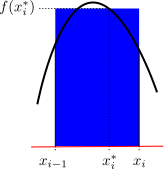
\includegraphics[width=\linewidth]{external/text/figs/rect_approx_adr2.pdf}
\end{sbspanel}%
\end{sidebyside}%
\item{}Thus the approximation to the integral, using all \(n\) subintervals, is%
\begin{gather*}
\int_a^b f(x)\dee{x}
\approx f(x_1^*)[x_1-x_0]+f(x_2^*)[x_2-x_1]+\cdots+ f(x_n^*)[x_n-x_{n-1}]
\end{gather*}
%
\item{}Of course every different choice of \(n\) and \(x_1,x_2,\cdots,x_{n-1}\)  and \(x_1^*, x_2^*,\cdots,x_n^*\) gives a different approximation. So to  simplify the  discussion that follows, let us denote a particular choice of all these numbers  by \(\bbbp\):%
\begin{gather*}
\bbbp=\left(n,x_1,x_2,\cdots,x_{n-1},x_1^*, x_2^*, \cdots, x_n^*\right).
\end{gather*}
Similarly let us denote the resulting approximation by \(\cI(\bbbp)\):%
\begin{gather*}
\cI(\bbbp)=f(x_1^*)[x_1-x_0]+f(x_2^*)[x_2-x_1]+\cdots+ f(x_n^*)[x_n-x_{n-1}]
\end{gather*}
%
\item{}We claim that, for any reasonable \footnote{We'll be more precise about  what ``reasonable'' means shortly.\label{fn-ssec_careful_defn-c-a-g-a}} function \(f(x)\), if you take any reasonable \footnote{Again, we'll explain this ``reasonable'' shortly\label{fn-ssec_careful_defn-c-a-g-c}} sequence  of  these  approximations you always get the exactly the same limiting value. We define  \(\int_a^b f(x) \dee{x}\) to be this limiting value.%
\item{}Let's be more precise. We can take the limit of these approximations in  two equivalent ways. Above we did this by taking the number of subintervals \(n\)  to infinity. When we did this, the width of all the subintervals went to zero.  With the formulation we are now using, simply taking the number of subintervals  to be very large does not imply that they will all shrink in size. We could  have  one very large subinterval and a large number of tiny ones. Thus we take the  limit we need by taking the width of the subintervals to zero. So for any  choice  \(\bbbp\), we define%
\begin{gather*}
M(\bbbp)=\max\big\{ x_1-x_0\ ,\  x_2-x_1\ ,\  \cdots\ ,\  x_n-x_{n-1}\big\}
\end{gather*}
that is the maximum width of the subintervals used in the approximation  determined by  \(\bbbp\). By forcing the maximum width to go to zero, the widths of all the  subintervals  go to zero.%
\item{}We then define the definite integral as the limit%
\begin{gather*}
\int_a^b f(x)\dee{x}=\lim_{M(\bbbp)\rightarrow 0}\cI(\bbbp).
\end{gather*}
%
\end{itemize}
Of course, one is now left with the question of determining when the above  limit  exists.  A proof of the very general conditions which guarantee existence of this limit  is beyond  the scope of this course, so we instead give a weaker result (with stronger  conditions)  which is far easier to prove.%
\par
For the rest of this section, assume%
\begin{itemize}[label=\textbullet]
\item{}that \(f(x)\) is continuous for \(a\le x\le b\),%
\item{}that \(f(x)\) is differentiable for \(a \lt x \lt b\), and%
\item{}that \(f'(x)\) is bounded \textemdash{} ie \(|f'(x)|\leq F\) for some constant \(F\).%
\end{itemize}
We will now show that, under these hypotheses, as \(M(\bbbp)\) approaches zero,  \(\cI(\bbbp)\)  always approaches the area, \(A\), between the graph of \(y=f(x)\) and the  \(x\)-axis, with \(x\)  running from \(a\) to \(b\).%
\par
These assumptions are chosen to make the argument particularly transparent.  With  a little  more work one can weaken the hypotheses considerably. We are cheating a little  by  implicitly assuming that the area \(A\) exists. In fact, one can adjust the  argument below  to remove this implicit assumption.%
\begin{itemize}[label=\textbullet]
\item{}Consider \(A_j\), the part of the area coming from \(x_{j-1}\le x\le x_j\).%
\begin{sidebyside}{1}{0.125}{0.125}{0}%
\begin{sbspanel}{0.75}%
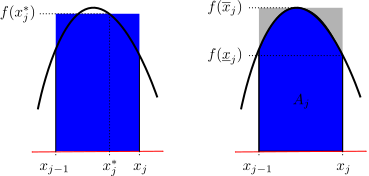
\includegraphics[width=\linewidth]{external/text/figs/rect_approx_adr3.pdf}
\end{sbspanel}%
\end{sidebyside}%
\par
We have approximated this area by \(f(x_j^*)[x_j-x_{j-1}]\) (see figure left).%
\item{}Let \(f({\overline x}_j)\) and  \(f({\underline x}_j)\) be the largest and smallest values \footnote{Here we are  using the  extreme value theorem \textemdash{} its proof is beyond the scope of this course. The  theorem says  that any continuous function on a closed interval must attain a minimum and  maximum at  least once. In this situation this implies that for any continuous function  \(f(x)\),  there are \(x_{j-1}\le {\overline x}_j, {\underline x}_j\le x_j\) such that \(f({\underline x}_j)\le f(x) \le f({\overline x}_j)\) for all \(x_{j-1}\le x\le x_j\).\label{fn-ssec_careful_defn-e-b-b-c}} of \(f(x)\) for \(x_{j-1}\le x\le x_j\). Then the true area is bounded by%
\begin{gather*}
f({\underline x}_j)[x_j-x_{j-1}] \leq  A_j \leq f({\overline x}_j)[x_j-x_{j-1}].
\end{gather*}
(see figure right).%
\item{}Now since \(f({\underline x}_j) \leq f(x_j^*) \leq f({\overline x}_j)\), we  also know  that%
\begin{gather*}
f({\underline x}_j)[x_j-x_{j-1}] \leq  f(x_j^*)[x_j-x_{j-1}] \leq f({\overline x}_j)[x_j-x_{j-1}].
\end{gather*}
%
\item{}So both the true area, \(A_j\), and our approximation of that area  \(f(x_j^*)[x_j - x_{j-1}]\)  have to lie between \(f({\overline  x}_j)[x_j-x_{j-1}]\) and \(f({\underline x}_j)[x_j-x_{j-1}]\). Combining these  bounds we have that the difference between the true area and our approximation  of that area is bounded by%
\begin{gather*}
\big|A_j-f(x_j^*)[x_j-x_{j-1}]\big| \le[f({\overline x}_j)-f({\underline x}_j)]\cdot[x_j-x_{j-1}].
\end{gather*}
(To see this think about the smallest the true area can be and the largest our  approximation can be and vice versa.)%
\item{}Now since our function, \(f(x)\) is differentiable we can apply one of the  main  theorems we learned in CLP-1 \textemdash{} the Mean Value  Theorem \footnote{Recall that the mean value theorem states that for a function  continuous on \([a,b]\) and differentiable on \((a,b)\), there exists a number \(c\)  between  \(a\) and \(b\) so that \(f'(c) = \frac{f(b)-f(a)}{b-a}.\)\label{fn-ssec_careful_defn-e-b-e-c}}. The MVT implies that there exists a \(c\) between \({\underline  x}_j\) and \({\overline x}_j\) such that%
\begin{gather*}
f({\overline x}_j)-f({\underline x}_j) =f'(c)\cdot [{\overline x}_j-{\underline x}_j]
\end{gather*}
%
\item{}By the assumption that \(|f'(x)|\le F\) for all \(x\) and the fact that  \({\underline  x}_j\) and \({\overline x}_j\) must both be between \(x_{j-1}\) and \(x_j\)%
\begin{gather*}
\big|f({\overline x}_j)-f({\underline x}_j)\big|
\le F\cdot \big|{\overline x}_j-{\underline x}_j\big|
\le F\cdot [x_j-x_{j-1}]
\end{gather*}
Hence the error in this part of our approximation obeys%
\begin{gather*}
\big|A_j-f(x_j^*)[x_j-x_{j-1}]\big|
\le F\cdot [x_j-x_{j-1}]^2.
\end{gather*}
%
\item{}That was just the error in approximating \(A_j\). Now we bound the total  error by  combining the errors from approximating on all the subintervals. This gives%
\begin{align*}
\left| A-\cI(\bbbp)\right|
&= \left| \sum_{j=1}^n A_j - \sum_{j=1}^n f(x_j^*)[x_j-x_{j-1}] \right|\\
&= \left| \sum_{j=1}^n \left(A_j - f(x_j^*)[x_j-x_{j-1}] \right) \right|
&\text{triangle inequality}\\
&\leq \sum_{j=1}^n\left|A_j - f(x_j^*)[x_j-x_{j-1}]\right|\\
&\leq \sum_{j=1}^n F\cdot [x_j-x_{j-1}]^2 & \text{from above}\\
\intertext{Now do something a little sneaky. Replace one of these factors of  \([x_j-x_{j-1}]\) (which is just the width of the \(j^\mathrm{th}\) subinterval) by the	maximum width of the subintervals:}
&\leq \sum_{j=1}^n F\cdot M(\bbbp)\cdot [x_j-x_{j-1}]  &\text{$F$ and  $M(\bbbp)$ are  constant}\\
&\leq F\cdot M(\bbbp)\cdot \sum_{j=1}^n [x_j-x_{j-1}] & \text{sum is total  width}\\
& = F\cdot M(\bbbp)\cdot (b-a).
\end{align*}
%
\item{}Since \(a\), \(b\) and \(F\) are fixed, this tends to zero as the maximum  rectangle width \(M(\bbbp)\) tends to zero.%
\end{itemize}
%
\par
Thus, we have proven%
\begin{theorem}{Theorem}{}{}{theorem-ssec_careful_defn-g}%
Assume that \(f(x)\) is continuous for \(a\le x\le b\), and is differentiable for all \(a \lt x \lt b\) with \(|f'(x)|\le F\), for some  constant \(F\).  Then,  as the maximum rectangle width \(M(\bbbp)\) tends to zero, \(\cI(\bbbp)\) always converges to \(A\), the area between the graph of \(y=f(x)\) and the \(x\)-axis,  with \(x\) running from \(a\) to \(b\).%
\end{theorem}
\end{subsectionptx}
%
%
\typeout{************************************************}
\typeout{Exercises 1.1.8 Exercises}
\typeout{************************************************}
%
\begin{exercises-subsection}{Exercises}{Exercises}{}{Exercises}{}{}{exercises-sec_intdef-j}
\par\medskip\noindent%
\textbf{.}\space\space%
For Questions~\hyperlink{exercise-concept_int_a}{1} through \hyperlink{exercise-concept_int_b}{5}, we want you to develop an understanding of the model we are using to define an integral: we approximate the area under a curve by bounding it between rectangles. Later, we will learn more sophisticated methods of integration, but they are all based on this simple concept.%
In Questions~\hyperlink{exercise-p1_1sigmaa}{6} through \hyperlink{exercise-p1_1sigmab}{10}, we practice using sigma notation. There are many ways to write a given sum in sigma notation. You can practice finding several, and deciding which looks the clearest.%
Questions~\hyperlink{exercise-p1_1Riemanna}{11} through \hyperlink{exercise-p1_1Riemannb}{15} are meant to give you practice interpreting the formulas in Definition~\hyperref[definition-def_INTthreeRiemannSums]{{\xreffont\ref{definition-def_INTthreeRiemannSums}}}. The formulas might look complicated at first, but if you understand what each piece means, they are easy to learn.%
\begin{exercisegroup}
\begin{divisionexerciseeg}{1}{}{}{exercise-concept_int_a}%
Give a range of possible values for the shaded area in the picture below.%
\begin{sidebyside}{1}{0.25}{0.25}{0}%
\begin{sbspanel}{0.5}%
\resizebox{\linewidth}{!}{%
\begin{tikzpicture}
\YEaaxis{1}{4}{1}{2}
\draw[thick, blue, fill] plot[domain=1:3, samples=100] (\x,{.25*sin(20*\x r)+1})--(3,0)--(1,0)--(1,1.23);
\YExcoord{1}{1};
\YExcoord{3}{3};
\YEycoord{0.75}{0.75};
\YEycoord{1.25}{1.25};
\foreach \x in {0.75,1.25}{\draw[dotted] (.2,\x)--(1,\x);}
\end{tikzpicture}
}%
\end{sbspanel}%
\end{sidebyside}%
\end{divisionexerciseeg}%
\begin{divisionexerciseeg}{2}{}{}{exercise-sec_intdef-j-a-e}%
Give a range of possible values for the shaded area in the picture below.%
\begin{sidebyside}{1}{0.25}{0.25}{0}%
\begin{sbspanel}{0.5}%
\resizebox{\linewidth}{!}{%
\begin{tikzpicture}
\YEaaxis{1.5}{5}{1}{3}
\draw[thick, blue, fill] plot[domain=1:1.96, samples=100] (\x,{.25*sin(20*\x r)+1})--
plot[domain=1.96:2.98, samples=100] (\x,{.25*sin(20*(\x-1.6) r )+2})--
plot[domain=2.98:4, samples=100] (\x,{.25*sin(20*\x r)+.5})--(4,0)--(1,0)--(1,1.23);
\YExcoord{1}{1};
\YExcoord{1.96}{2};
\YExcoord{2.98}{3};
\YExcoord{4}{4};
\YEycoord{0.75}{0.75};
\YEycoord{1.25}{1.25};
\YEycoord{0.25}{0.25};
\YEycoord{2.25}{2.25};
\YEycoord{1.75}{1.75};
\foreach \x in {0.75, 0.25}{\draw[dotted] (.2,\x)--(3.2,\x);}
\foreach \x in {1.75,2.25}{\draw[dotted] (.2,\x)--(2,\x);}
\foreach \x in {1.25}{\draw[dotted] (.2,\x)--(1,\x);}
\end{tikzpicture}
}%
\end{sbspanel}%
\end{sidebyside}%
\end{divisionexerciseeg}%
\begin{divisionexerciseeg}{3}{}{}{exercise-sec_intdef-j-a-f}%
Using rectangles, find a lower and upper bound for \(\displaystyle\int_1^3 \dfrac{1}{2^x}\dee{x}\) that differ by at most 0.2 square units.%
\begin{sidebyside}{1}{0.335}{0.335}{0}%
\begin{sbspanel}{0.33}%
\resizebox{\linewidth}{!}{%
\begin{tikzpicture}
\YEaaxis{1}{5}{1}{5}
\draw[thick, blue, fill] plot[domain=1:3, samples=100] (\x,{6*pow(.5,\x)})--(3,0)--(1,0)--cycle;
\draw[thick] plot[domain=0.5:4, samples=100] (\x,{6*pow(.5,\x)}) node[above right]{$y=\frac{1}{2^x}$};
\YExcoord{1}{1};
\YExcoord{3}{3};
\draw[thick] (1,0)--(1,3) (3,0)--(3,.75);
\end{tikzpicture}
}%
\end{sbspanel}%
\end{sidebyside}%
\end{divisionexerciseeg}%
\begin{divisionexerciseeg}{4}{}{}{exercise-sec_intdef-j-a-g}%
Let \(f(x)\) be a function that is \emph{decreasing} from \(x=0\) to \(x=5\). Which Riemann sum approximation of \(\displaystyle\int_0^5 f(x)\dee{x}\) is the largest-{}-{}left, right, or midpoint?%
\end{divisionexerciseeg}%
\begin{divisionexerciseeg}{5}{}{}{exercise-concept_int_b}%
Give an example of a function \(f(x)\), an interval \([a,b]\), and a number \(n\) such that the midpoint Riemann sum of \(f(x)\) over \([a,b]\) using \(n\) intervals is \emph{larger than} both the left and right Riemann sums  of \(f(x)\) over \([a,b]\) using \(n\) intervals.%
\end{divisionexerciseeg}%
\begin{divisionexerciseeg}{6}{}{}{exercise-p1_1sigmaa}%
Express the following sums in sigma notation:%
\begin{enumerate}[label=\alph*]
\item{}\(\displaystyle 3+4+5+6+7\)%
\item{}\(\displaystyle 6+8+10+12+14\)%
\item{}\(\displaystyle 7+9+11+13+15\)%
\item{}\(\displaystyle 1+3+5+7+9+11+13+15\)%
\end{enumerate}
%
\end{divisionexerciseeg}%
\begin{divisionexerciseeg}{7}{}{}{exercise-p1_1powers}%
Express the following sums in sigma notation:%
\begin{enumerate}[label=\alph*]
\item{}\(\displaystyle \frac{1}{3}+\frac{1}{9}+\frac{1}{27}+\frac{1}{81}\)%
\item{}\(\displaystyle \frac{2}{3}+\frac{2}{9}+\frac{2}{27}+\frac{2}{81}\)%
\item{}\(\displaystyle -\frac{2}{3}+\frac{2}{9}-\frac{2}{27}+\frac{2}{81}\)%
\item{}\(\displaystyle \frac{2}{3}-\frac{2}{9}+\frac{2}{27}-\frac{2}{81}\)%
\end{enumerate}
%
\end{divisionexerciseeg}%
\begin{divisionexerciseeg}{8}{}{}{exercise-sec_intdef-j-a-l}%
Express the following sums in sigma notation:%
\begin{enumerate}[label=\alph*]
\item{}\(\displaystyle \frac{1}{3}+\frac{1}{3}+\frac{5}{27}+\frac{7}{81}+\frac{9}{243}\)%
\item{}\(\displaystyle \frac{1}{5}+\frac{1}{11}+\frac{1}{29}+\frac{1}{83}+\frac{1}{245}\)%
\item{}\(\displaystyle 1000+200+30+4+\frac{1}{2}+\frac{3}{50}+\frac{7}{1000}\)%
\end{enumerate}
%
\end{divisionexerciseeg}%
\begin{divisionexerciseeg}{9}{}{}{exercise-sec_intdef-j-a-m}%
Evaluate the following sums. You might want to use the formulas from Theorems ~\hyperref[theorem-thm_INTsummationArith]{5} and \hyperref[theorem-thm_INTspecialSums]{6}.%
\begin{enumerate}[label=\alph*]
\item{}\(\displaystyle \displaystyle\sum_{i=0}^{100} \left(\dfrac{3}{5}\right)^i\)%
\item{}\(\displaystyle \displaystyle\sum_{i=50}^{100} \left(\dfrac{3}{5}\right)^i\)%
\item{}\(\displaystyle \displaystyle\sum_{i=1}^{10} \left(i^2-3i+5\right)\)%
\item{}\(\displaystyle\sum_{n=1}^{b}\left[ \left(\frac{1}{e}\right)^n+en^3\right]\), where \(b\) is some integer greater than 1.%
\end{enumerate}
%
\end{divisionexerciseeg}%
\begin{divisionexerciseeg}{10}{}{}{exercise-p1_1sigmab}%
Evaluate the following sums. You might want to use the formulas from Theorem~\hyperref[theorem-thm_INTspecialSums]{{\xreffont\ref{theorem-thm_INTspecialSums}}}.%
\begin{enumerate}[label=\alph*]
\item{}\(\displaystyle \displaystyle\sum_{i=50}^{100} (i-50)+\displaystyle\sum_{i=0}^{50} i\)%
\item{}\(\displaystyle \displaystyle\sum_{i=10}^{100} \left(i-5\right)^3\)%
\item{}\(\displaystyle \displaystyle\sum_{n=1}^{11} (-1)^n\)%
\item{}\(\displaystyle \displaystyle\sum_{n=2}^{11} (-1)^{2n+1}\)%
\end{enumerate}
%
\end{divisionexerciseeg}%
\begin{divisionexerciseeg}{11}{}{}{exercise-p1_1Riemanna}%
In the picture below, draw in the rectangles whose (signed) area is being computed by the midpoint Riemann sum \(\displaystyle\sum_{i=1}^4 \dfrac{b-a}{4}\cdot f\left(a+\left(i-\frac{1}{2}\right)\dfrac{b-a}{4}\right)\).%
\begin{sidebyside}{1}{0.25}{0.25}{0}%
\begin{sbspanel}{0.5}%
\resizebox{\linewidth}{!}{%
\begin{tikzpicture}
\YEaxis{4}{3};
\YExcoord{2.5}{b}
\YExcoord{-2.5}{a}
\draw[very thick] (-3,-3) .. controls (-1.5,4) and (1,-2) .. (3,3) node[right]{$y=f(x)$};
\end{tikzpicture}
}%
\end{sbspanel}%
\end{sidebyside}%
\end{divisionexerciseeg}%
\begin{divisionexerciseeg}{12}{M105 2015A.}{}{exercise-sec_intdef-j-a-q}%
\(\displaystyle \sum_{k=1}^4 f(1+k)\cdot 1\) is a left Riemann sum for a function \(f(x)\) on the interval \([a,b]\) with \(n\) subintervals. Find the values of \(a\), \(b\) and \(n\).%
\end{divisionexerciseeg}%
\begin{divisionexerciseeg}{13}{}{}{exercise-p1_1RiemannInterp}%
Draw a picture illustrating the area given by the following Riemann sum.%
\begin{equation*}
\sum_{i=1}^3 2\cdot\left(5+2i\right)^2 
\end{equation*}
%
\end{divisionexerciseeg}%
\begin{divisionexerciseeg}{14}{}{}{exercise-sec_intdef-j-a-s}%
Draw a picture illustrating the area given by the following Riemann sum.%
\begin{equation*}
\sum_{i=1}^5 \frac{\pi}{20}\cdot \tan\left(\frac{\pi (i-1)}{20}\right)
\end{equation*}
%
\end{divisionexerciseeg}%
\begin{divisionexerciseeg}{15}{M105 2013A.}{}{exercise-p1_1Riemannb}%
Fill in the blanks with right, left, or midpoint; an interval; and a value of n.%
\par
%
\begin{enumerate}[label=\alph*]
\item{}\(\sum\limits_{k=0}^3 f (1.5 + k) \cdot 1\) is a \(\underline{\ \ \ \ \ \ \ \ \ \ \ \ }\) Riemann sum for \(f\) on the interval \([\,\underline{\ \ \ \ \ \ }\ ,\ \underline{\ \ \ \ \ \ }\,]\) with \(n =\underline{\ \ \ \ \ }\).%
\end{enumerate}
%
\end{divisionexerciseeg}%
\begin{divisionexerciseeg}{16}{}{}{exercise-sec_intdef-j-a-u}%
Evaluate the following integral by interpreting it as a signed area, and using geometry:%
\begin{equation*}
\int_0^5 x \,\dee{x}
\end{equation*}
%
\end{divisionexerciseeg}%
\begin{divisionexerciseeg}{17}{}{}{exercise-sec_intdef-j-a-v}%
Evaluate the following integral by interpreting it as a signed area, and using geometry:%
\begin{equation*}
\int_{-2}^5 x \,\dee{x}
\end{equation*}
%
\end{divisionexerciseeg}%
\end{exercisegroup}
\par\medskip\noindent
\par\medskip\noindent%
\textbf{.}\space\space%
Questions~\hyperlink{exercise-p1_1geoma}{26} and \hyperlink{exercise-p1_1geomb}{27} use the formula for a geometric sum, Equation~\hyperref[fact-eq_INTgeomsum]{{\xreffont\ref{fact-eq_INTgeomsum}}}%
Remember that a definite integral is a signed area between a curve and the \(x\)-axis. We'll spend a lot of time learning strategies for evaluating definite integrals, but we already know lots of ways to find area of geometric shapes. In Questions~\hyperlink{exercise-p1_1defintgeoma}{28} through \hyperlink{exercise-p1_1defintgeomb}{33}, use your knowledge of geometry to find the signed areas described by the integrals given.%
\begin{exercisegroup}
\begin{divisionexerciseeg}{18}{M105 2014A.}{}{exercise-sec_intdef-j-b-c}%
Use sigma notation to write the midpoint Riemann sum for \(f(x)=x^8\) on \([5,15]\) with \(n=50\). Do not evaluate the Riemann sum.%
\end{divisionexerciseeg}%
\begin{divisionexerciseeg}{19}{2016Q1.}{}{exercise-sec_intdef-j-b-d}%
Estimate \(\displaystyle\int_{-1}^5 x^3\,\,\dee{x}\) using three approximating rectangles and left hand end points.%
\end{divisionexerciseeg}%
\begin{divisionexerciseeg}{20}{2016Q1.}{}{exercise-sec_intdef-j-b-e}%
Let \(f\) be a function on the whole real line.  Express \(\displaystyle\int_{-1}^{7}f(x)\,\,\dee{x}\) as a limit of Riemann sums, using the right endpoints.%
\end{divisionexerciseeg}%
\begin{divisionexerciseeg}{21}{2016Q1.}{}{exercise-sec_intdef-j-b-f}%
The value of the following limit is equal to the area below a graph of \(y=f(x)\), integrated over the interval \([0,b]\):%
\begin{gather*}
\lim_{n \to \infty} \sum_{i=1}^{n} \frac{4}{n}
\left[ \sin \left( 2 + \frac{4i}{n}\right)\right]^2
\end{gather*}
Find \(f(x)\) and \(b\).%
\end{divisionexerciseeg}%
\begin{divisionexerciseeg}{22}{M105 2102A.}{}{exercise-sec_intdef-j-b-g}%
For a certain function \(f(x)\), the following equation holds:%
\begin{equation*}
\lim_{n\rightarrow\infty}\sum\limits_{k=1}^n
\frac{k}{n^2}\sqrt{1-\frac{k^2}{n^2}}
=\int_0^1 f(x)\ \,\dee{x}
\end{equation*}
Find \(f(x)\).%
\end{divisionexerciseeg}%
\begin{divisionexerciseeg}{23}{2016Q1.}{}{exercise-sec_intdef-j-b-h}%
Express \(\displaystyle\lim_{n\to\infty}\displaystyle\sum_{i=1}^{n}
\frac{3}{n} e^{-i/n} \cos\left(\frac{3i}{n}\right)\) as a definite integral.%
\end{divisionexerciseeg}%
\begin{divisionexerciseeg}{24}{2012A, 2014D.}{}{exercise-sec_intdef-j-b-i}%
Let \(\displaystyle R_n= \sum_{i=1}^{n}
\frac{i e^{i/n}}{n^2}\). Express \(\displaystyle\lim_{n\to\infty}R_n\) as a definite integral. \emph{Do not evaluate this integral.}%
\end{divisionexerciseeg}%
\begin{divisionexerciseeg}{25}{2016A.}{}{exercise-sec_intdef-j-b-j}%
Express \(\displaystyle\lim_{n\rightarrow\infty} \bigg( \sum_{i=1}^n e^{-1-2i/n}\cdot \frac{2}{n} \bigg)\) as an integral in three different ways.%
\end{divisionexerciseeg}%
\begin{divisionexerciseeg}{26}{}{}{exercise-p1_1geoma}%
Evaluate the sum \(1+r^3+r^6+r^9+\cdots+r^{3n}\).%
\end{divisionexerciseeg}%
\begin{divisionexerciseeg}{27}{}{}{exercise-p1_1geomb}%
Evaluate the sum \(r^5+r^6+r^7+\cdots+r^{100}\).%
\end{divisionexerciseeg}%
\begin{divisionexerciseeg}{28}{M105 2013A.}{}{exercise-p1_1defintgeoma}%
Evaluate \({\displaystyle\int_{-1}^2 |2x|\ \,\dee{x}}\).%
\end{divisionexerciseeg}%
\begin{divisionexerciseeg}{29}{}{}{exercise-sec_intdef-j-b-p}%
Evaluate the following integral by interpreting it as a signed area, and using geometry:%
\begin{equation*}
\int_{-3}^5 |t-1| \,\dee{t}
\end{equation*}
%
\end{divisionexerciseeg}%
\begin{divisionexerciseeg}{30}{}{}{exercise-p1_1trapezoidarea}%
Evaluate the following integral by interpreting it as a signed area, and using geometry:%
\begin{equation*}
\int_a^b x \,\dee{x}
\end{equation*}
%
\par
where \(0 \leq a \leq b\).%
\end{divisionexerciseeg}%
\begin{divisionexerciseeg}{31}{}{}{exercise-sec_intdef-j-b-r}%
Evaluate the following integral by interpreting it as a signed area, and using geometry:%
\begin{equation*}
\int_a^b x\, \dee{x}
\end{equation*}
%
\par
where \(a \leq b \leq 0\).%
\end{divisionexerciseeg}%
\begin{divisionexerciseeg}{32}{}{}{exercise-sec_intdef-j-b-s}%
Evaluate the following integral by interpreting it as a signed area, and using geometry:%
\begin{equation*}
\int_0^4 \sqrt{16-x^2} \dee{x}
\end{equation*}
%
\end{divisionexerciseeg}%
\begin{divisionexerciseeg}{33}{2016Q1.}{}{exercise-p1_1defintgeomb}%
Use elementary geometry to calculate \(\displaystyle \int_0^3 f(x)\,\,\dee{x}\), where%
\begin{align*}
f(x) = \begin{cases}
x, & \text{if } x \le 1,\\
1, & \text{if } x  \gt  1.
\end{cases}
\end{align*}
%
\end{divisionexerciseeg}%
\begin{divisionexerciseeg}{34}{2016Q1.}{}{exercise-p1_1cartime}%
A car's gas pedal is applied at \(t=0\) seconds and the car accelerates continuously until \(t=2\) seconds. The car's speed at half-second intervals is given in the table below. Find the best possible \alert{upper} estimate for the distance that the car traveled during these two seconds.%
\begin{sidebyside}{1}{0}{0}{0}%
\begin{sbspanel}{1}%
\resizebox{\ifdim\width > \linewidth\linewidth\else\width\fi}{!}{%
{\centering%
{\tabularfont%
\begin{tabular}{AlAlAlAlAlAlA}\hrulethin
\(t\) (s)&\(0\)&\(0.5\)&\(1.0\)&\(1.5\)&\(2\)\tabularnewline\hrulethin
\(v\) (m\slash{}s)&0&14&22&30&40\tabularnewline\hrulethin
\end{tabular}
}%
\par}
}%
\end{sbspanel}%
\end{sidebyside}%
\end{divisionexerciseeg}%
\begin{divisionexerciseeg}{35}{}{}{exercise-sec_intdef-j-b-v}%
True or false: the answer you gave for Question~\hyperlink{exercise-p1_1cartime}{34} is definitely greater than or equal to the distance the car travelled during the two seconds in question.%
\end{divisionexerciseeg}%
\begin{divisionexerciseeg}{36}{}{}{exercise-p1_1airtime}%
An airplane's speed at one-hour intervals is given in the table below. Approximate the distance travelled by the airplane from noon to 4pm using a midpoint Riemann sum.%
\begin{sidebyside}{1}{0}{0}{0}%
\begin{sbspanel}{1}%
\resizebox{\ifdim\width > \linewidth\linewidth\else\width\fi}{!}{%
{\centering%
{\tabularfont%
\begin{tabular}{AlAlAlAlAlAlA}\hrulethin
time&12:00 pm&1:00 pm&2:00 pm&3:00 pm&4:00 pm\tabularnewline\hrulethin
speed (km\slash{}hr)&800&700&850&900&750\tabularnewline\hrulethin
\end{tabular}
}%
\par}
}%
\end{sbspanel}%
\end{sidebyside}%
\end{divisionexerciseeg}%
\end{exercisegroup}
\par\medskip\noindent
\par\medskip\noindent%
\textbf{.}\space\space%
\begin{exercisegroup}
\begin{divisionexerciseeg}{37}{2016Q1.}{}{exercise-sec_intdef-j-c-c}%
(a) Express%
\begin{equation*}
\lim_{n\rightarrow\infty}
\sum_{i=1}^n\frac{2}{n}\sqrt{4-\left(-2+\frac{2i}{n}\right)^2}
\end{equation*}
as a definite integal.%
\par
(b) Evaluate the integral of part (a).%
\end{divisionexerciseeg}%
\begin{divisionexerciseeg}{38}{2016Q1.}{}{exercise-sec_intdef-j-c-d}%
Consider the integral:%
\begin{gather*}
\int_0^3 (7 + x^3) \,\,\dee{x} .\qquad\qquad (*)
\end{gather*}
%
\begin{enumerate}[label=\alph*]
\item{}Approximate this integral using the left Riemann sum with \(n=3\) intervals.%
\item{}Write down the expression for the right Riemann sum with \(n\) intervals and calculate the sum. Now take the limit \(n \to \infty\) in your expression for the Riemann sum, to evaluate the integral (\(*\)) exactly.%
\end{enumerate}
You may use the identity%
\begin{gather*}
\sum_{i=1}^{n} i^3 = \frac{n^4 +2n^3 + n^2}{4}
\end{gather*}
%
\end{divisionexerciseeg}%
\begin{divisionexerciseeg}{39}{2013A.}{}{exercise-sec_intdef-j-c-e}%
Using a limit of right-{}-{}endpoint Riemann sums, evaluate \(\displaystyle\int_2^4 x^2\ \,\dee{x}\). You may use the formulas \(\sum\limits_{i=1}^n i = \frac{n(n + 1)}{2}\) and \(\sum\limits_{i=1}^n i^2 = \frac{n(n + 1)(2n + 1)}{6}\).%
\end{divisionexerciseeg}%
\begin{divisionexerciseeg}{40}{2016Q1.}{}{exercise-sec_intdef-j-c-f}%
Find \(\displaystyle\int_0^2 (x^3+x)\,\,\dee{x}\) using the definition of the definite integral. You may use the summation formulas \(\sum\limits_{i=1}^{n}i^3 = \frac{n^4+2n^3+n^2}4\) and \(\sum\limits_{i=1}^{n} i = \frac{n^2+n}{2}\).%
\end{divisionexerciseeg}%
\begin{divisionexerciseeg}{41}{2014D.}{}{exercise-sec_intdef-j-c-g}%
Using a limit of right-endpoint Riemann sums, evaluate \(\displaystyle\int_1^4 (2x-1)\,\,\dee{x}\). Do not use  anti-differentiation, except to check your answer. \footnotemark{} You may use the formula \(\sum\limits_{i=1}^{n} i = \frac{n(n+1)}{2}\).%
\end{divisionexerciseeg}%
\footnotetext[25]{You'll learn about this method starting in Section~\hyperref[section-sec_fundamental]{{\xreffont\ref{section-sec_fundamental}}}. You can also check this answer using geometry.\label{fn-sec_intdef-j-c-g-b-a-b}}%
\begin{divisionexerciseeg}{42}{}{}{exercise-sec_intdef-j-c-h}%
Give a function \(f(x)\) that has the following expression as a right Riemann sum when \(n=10\), \(\Delta(x)=10\) and \(a=-5\):%
\begin{equation*}
\sum_{i=1}^{10} 3(7+2i)^2\sin(4i)\,.
\end{equation*}
%
\end{divisionexerciseeg}%
\begin{divisionexerciseeg}{43}{}{}{exercise-p1_1_2x}%
Using the method of Example~\hyperref[example-eg_INTexpareaB]{{\xreffont\ref{example-eg_INTexpareaB}}}, evaluate%
\begin{equation*}
\int_0^1 2^x \dee{x}
\end{equation*}
%
\end{divisionexerciseeg}%
\begin{divisionexerciseeg}{44}{}{}{exercise-sec_intdef-j-c-j}%
%
\begin{enumerate}[label=\alph*]
\item{}Using the method of Example~\hyperref[example-eg_INTexpareaB]{{\xreffont\ref{example-eg_INTexpareaB}}}, evaluate%
\begin{equation*}
\int_a^b 10^x \dee{x}
\end{equation*}
%
\item{}%
\end{enumerate}
Using your answer from above, make a guess for%
\begin{equation*}
\int_a^b c^x \dee{x}
\end{equation*}
%
\par
where \(c\) is a positive constant. Does this agree with Question~\hyperlink{exercise-p1_1_2x}{43}?%
\end{divisionexerciseeg}%
\begin{divisionexerciseeg}{45}{}{}{exercise-p1_1_awkwardcircle}%
Evaluate \(\displaystyle\int_0^a \sqrt{1-x^2}\dee{x}\) using geometry, if \(0 \leq a \leq 1\).%
\end{divisionexerciseeg}%
\begin{divisionexerciseeg}{46}{}{}{exercise-p1_1errornotaylor}%
Suppose \(f(x)\) is a positive, decreasing function from \(x=a\) to \(x=b\). You give an upper and lower bound on the area under the curve \(y=f(x)\) using \(n\) rectangles and a left and right Riemann sum, respectively, as in the picture below.%
\begin{sidebyside}{2}{0.05}{0.05}{0.1}%
\begin{sbspanel}{0.4}%
\resizebox{\linewidth}{!}{%
\begin{tikzpicture}[scale=0.8]
\YEaaxis{1}{7.5}{1}{5}
\draw[red, pattern=crosshatch, pattern color=red] (1,0)--(1,4.25)-|(2,2.9)-|(3,1.85)-|(4,1.1)-|(5,0.65)-|(6,0.5)-|(6,0)--cycle;
\draw[thick] plot[domain=0.75:6.25, samples=100] (\x,{.15*(\x-6)*(\x-6)+.5}) node[right]{$y=f(x)$};
\draw[ fill=black, fill opacity=0.25] (1,0)--plot[domain=1:6, samples=100] (\x,{.15*(\x-6)*(\x-6)+.5}) --(6,0)--cycle;
\foreach \x in {1,...,6}{
\SUBTRACT{\x}{6}{\y}
\MULTIPLY{\y}{\y}{\z}
\MULTIPLY{\z}{0.15}{\w}
\ADD{\w}{0.5}{\c}
\draw[red, thick] (\x,0)--(\x,\c);}
\YExcoord{1}{a};
\YExcoord{6}{b};
\end{tikzpicture}
}%
\end{sbspanel}%
\begin{sbspanel}{0.4}%
\resizebox{\linewidth}{!}{%
\begin{tikzpicture}[scale=0.8]
\YEaaxis{1}{7.5}{1}{5}
\draw[red, pattern=crosshatch, pattern color=red] (1,0)--(1,2.9)-|(2,1.859)-|(3,1.1)-|(4,0.65)-|(5,0.5)-|(6,0)--cycle;
\draw[thick] plot[domain=0.75:6.25, samples=100] (\x,{.15*(\x-6)*(\x-6)+.5}) node[right]{$y=f(x)$};
\draw[fill=black, fill opacity=0.25] (1,0)--plot[domain=1:6, samples=100] (\x,{.15*(\x-6)*(\x-6)+.5}) --(6,0)--cycle;
\foreach \x in {2,...,6}{
\SUBTRACT{\x}{6}{\y}
\MULTIPLY{\y}{\y}{\z}
\MULTIPLY{\z}{0.15}{\w}
\ADD{\w}{0.5}{\c}
\draw[red, thick] (\x,0)--(\x,\c);}
\YExcoord{1}{a};
\YExcoord{6}{b};
\end{tikzpicture}
}%
\end{sbspanel}%
\end{sidebyside}%
\par
%
\begin{enumerate}[label=\alph*]
\item\hypertarget{li-riemannerrorbounda}{}What is the difference between the lower bound and the upper bound? (That is, if we subtract the smaller estimate from the larger estimate, what do we get?) Give your answer in terms of \(f\), \(a\),  \(b\), and \(n\).%
\item{}If you want to approximate the area under the curve to within 0.01 square units using this method, how many rectangles should you use? That is, what should \(n\) be?%
\end{enumerate}
%
\end{divisionexerciseeg}%
\begin{divisionexerciseeg}{47}{}{}{exercise-sec_intdef-j-c-m}%
Let \(f(x)\) be a linear function,  let \(a \lt b\) be integers, and let \(n\) be a whole number. True or false: if we average the left and right Riemann sums for \(\displaystyle\int_a^b f(x)\dee{x}\) using \(n\) rectangles, we get the same value as the midpoint Riemann sum using \(n\) rectangles.%
\end{divisionexerciseeg}%
\end{exercisegroup}
\par\medskip\noindent
\end{exercises-subsection}
\end{sectionptx}
%
%
\typeout{************************************************}
\typeout{Section 1.2 Basic properties of the definite integral}
\typeout{************************************************}
%
\begin{sectionptx}{Section}{Basic properties of the definite integral}{}{Basic properties of the definite integral}{}{}{section-sec_def_int}
\begin{introduction}{}%
When we studied limits and derivatives, we developed methods for taking limits  or derivatives of ``complicated functions'' like \(f(x)=x^2 + \sin(x)\) by  understanding how limits and derivatives interact with basic arithmetic  operations like addition and subtraction. This allowed us to reduce the problem  into one of of computing derivatives of simpler functions like \(x^2\) and  \(\sin(x)\). Along the way we established  simple rules such as%
\begin{gather*}
\lim_{x\to a}(f(x)+g(x)) = \lim_{x\to a}f(x) + \lim_{x\to a} g(x)
\quad\text{and}\quad
\diff{}{x}(f(x)+g(x)) = \diff{f}{x} + \diff{g}{x}
\end{gather*}
Some of these rules have very natural analogues for integrals and we discuss  them below. Unfortunately the analogous rules for integrals of products of  functions or integrals of compositions of functions are more complicated than  those for limits or derivatives. We discuss those rules at length in subsequent  sections. For now let us consider some of the simpler rules of the arithmetic  of  integrals.%
\begin{theorem}{Theorem}{Arithmetic of Integration.}{}{theorem-thm_Intarith}%
Let \(a,b\) and \(A,B,C\) be real numbers. Let the functions \(f(x)\) and \(g(x)\) be integrable on an interval that contains \(a\) and \(b\). Then%
\begin{align*}
\text{(a)}&& \int_a^b \left( f(x) + g(x) \right)\dee{x} &= \int_a^b f(x)\dee{x} + \int_a^b g(x)\dee{x}\\
\text{(b)}&& \int_a^b\left(f(x)-g(x)\right)\dee{x}  &= \int_a^b f(x)\dee{x} - \int_a^b g(x)\dee{x}\\
\text{(c)}&& \int_a^b C f(x) \dee{x} &= C\cdot \int_a^b f(x)\dee{x}\\
\intertext{Combining these three rules we have}
\text{(d)}&& \int_a^b \left( Af(x) + Bg(x) \right)\dee{x} &= A\int_a^b f(x)\dee{x} + B\int_a^b g(x)\dee{x}\\
\intertext{That is, integrals depend linearly on the integrand.}
\text{(e)}&& \int_a^b \dee{x} = \int_a^b 1 \cdot \dee{x} &= b-a
\end{align*}
%
\end{theorem}
It is not too hard to prove this result from the definition of the definite  integral.  Additionally we only really need to prove (d) and (e) since%
\begin{itemize}[label=\textbullet]
\item{}(a) follows from (d) by setting \(A=B=1\),%
\item{}(b) follows from (d) by setting \(A=1, B=-1\), and%
\item{}(c) follows from (d) by setting \(A=C, B=0\).%
\end{itemize}
%
\begin{proof}{Proof}{}{proof-sec_def_int-b-d}
As noted above, it suffices for us to prove (d) and (e). Since (e) is easier,  we  will  start with that. It is also a good warm-up for (d).%
\begin{itemize}[label=\textbullet]
\item{}The definite integral in (e), \(\int_a^b 1 \dee{x}\), can be interpreted  geometrically as the area of the rectangle with height 1 running from \(x=a\) to  \(x=b\); this area is clearly \(b-a\). We can also prove this formula from the definition of  the  integral  (Definition~\hyperref[definition-def_INTintegral]{{\xreffont\ref{definition-def_INTintegral}}}):%
\begin{align*}
\int_a^b\dee{x}
&=\lim_{n\rightarrow\infty}\sum_{i=1}^n f(x_{i,n}^*)\,\frac{b-a}{n}
&\text{by definition}\\
&=\lim_{n\rightarrow\infty}\sum_{i=1}^n 1\,\frac{b-a}{n}
&\text{since $f(x)=1$}\\
&=\lim_{n\rightarrow\infty}(b-a) \sum_{i=1}^n \frac{1}{n}
&\text{since $a,b$ are constants}\\
&=\lim_{n\rightarrow\infty}(b-a)\\
&=b-a
\end{align*}
as required.%
\item{}To prove (d) let us start by defining \(h(x) = Af(x)+Bg(x)\) and then we  need to  express the integral of \(h(x)\) in terms of those of \(f(x)\) and \(g(x)\). We use  Definition~\hyperref[definition-def_INTintegral]{{\xreffont\ref{definition-def_INTintegral}}} and some algebraic manipulations \footnote{Now  is a good  time to look back at Theorem~\hyperref[theorem-thm_INTsummationArith]{{\xreffont\ref{theorem-thm_INTsummationArith}}}.\label{fn-sec_def_int-b-d-a-a-b-g}} to arrive at the  result.%
\begin{align*}
\int_a^bh(x) \dee{x}
&= \sum_{i=1}^n h(x_{i,n}^*)\cdot\frac{b-a}{n}\\
&\hskip0.5in\text{by Definition }\hyperref[definition-def_INTintegral]{\text{{\xreffont\ref{definition-def_INTintegral}}}}\\
&= \sum_{i=1}^n \left(Af(x_{i,n}^*)+Bg(x_{i,n}^*) \right)\cdot \frac{b-a}{n}\\
&= \sum_{i=1}^n \left(Af(x_{i,n}^*)\cdot \frac{b-a}{n} + Bg(x_{i,n}^*)\cdot
\frac{b-a}{n} \right)\\
&= \left(\sum_{i=1}^n Af(x_{i,n}^*)\cdot \frac{b-a}{n}\right)
+ \left(\sum_{i=1}^n Bg(x_{i,n}^*)\cdot \frac{b-a}{n}\right)\\
&\hskip0.5in\text{by Theorem }\hyperref[theorem-thm_INTsummationArith]{\text{{\xreffont\ref{theorem-thm_INTsummationArith}}}}\text{(b)}\\
&= A\left(\sum_{i=1}^n f(x_{i,n}^*)\cdot \frac{b-a}{n}\right)
+ B\left(\sum_{i=1}^n g(x_{i,n}^*)\cdot \frac{b-a}{n}\right)\\
&\hskip0.5in\text{by Theorem }\hyperref[theorem-thm_INTsummationArith]{\text{{\xreffont\ref{theorem-thm_INTsummationArith}}}}\text{(a)}\\
&= A \int_a^b f(x) \dee{x} + B \int_a^b g(x) \dee{x}\\
&\hskip0.5in\text{by Definition }\hyperref[definition-def_INTintegral]{\text{{\xreffont\ref{definition-def_INTintegral}}}}
\end{align*}
as required.%
\end{itemize}
%
\end{proof}
Using this Theorem we can integrate sums, differences and constant multiples of  functions  we know how to integrate. For example:%
\begin{example}{Example}{The integral of a sum.}{example-sec_def_int-b-f}%
In Example~\hyperref[example-eg_INTexparea]{{\xreffont\ref{example-eg_INTexparea}}} we saw that \(\int_0^1 e^x\dee{x}=e-1\). So%
\begin{align*}
\int_0^1\big(e^x+7\big)\dee{x} &= \int_0^1 e^x\dee{x} + 7\int_0^1 1 \dee{x}\\
& \text{by Theorem }\hyperref[theorem-thm_Intarith]{\text{{\xreffont\ref{theorem-thm_Intarith}}}}\text{(d) with $A=1,f(x)=e^x,B=7,g(x)=1$}\\
&=(e-1)+7\times (1-0)\\
&\text{by Example }\hyperref[example-eg_INTexparea]{\text{{\xreffont\ref{example-eg_INTexparea}}}}\text{ and  Theorem }\hyperref[theorem-thm_Intarith]{\text{{\xreffont\ref{theorem-thm_Intarith}}}}\text{(e)}\\
&=e+6
\end{align*}
%
\end{example}
When we gave the formal definition of \(\int_a^b f(x) \dee{x}\) in  Definition~\hyperref[definition-def_INTintegral]{{\xreffont\ref{definition-def_INTintegral}}} we explained that the integral could be  interpreted as the signed area between the curve \(y=f(x)\) and the \(x\)-axis on  the interval \([a,b]\). In order for this interpretation to make sense we  required  that \(a \lt b\), and though we remarked that the integral makes sense when \(a \gt b\) we  did not explain any further. Thankfully there is an easy way to express the  integral \(\int_a^b f(x)\dee{x}\) in terms of \(\int_b^a f(x)\dee{x}\) \textemdash{} making  it  always possible to write an integral so the lower limit of integration  is less than the upper limit of integration. Theorem~\hyperref[theorem-thm_Intdomain]{{\xreffont\ref{theorem-thm_Intdomain}}},  below,  tell us that, for example, \(\int_7^3 e^x\dee{x} = - \int_3^7 e^x\dee{x}\). The same theorem also provides us with two other simple manipulations of the limits of  integration.%
\begin{theorem}{Theorem}{Arithmetic for the Domain of Integration.}{}{theorem-thm_Intdomain}%
Let \(a,b,c\)  be real numbers. Let the function \(f(x)\)  be integrable on an interval that contains \(a\), \(b\) and \(c\). Then%
\begin{align*}
\text{(a)}&& \int_a^a f(x)\dee{x}&= 0\\
\text{(b)}&& \int_b^a f(x)\dee{x}&= -\int_a^b f(x)\dee{x}\\
\text{(c)}&& \int_a^b f(x)\dee{x}&= \int_a^c f(x)\dee{x} + \int_c^b f(x)\dee{x}
\end{align*}
%
\end{theorem}
The proof of this statement is not too difficult.%
\begin{proof}{Proof}{}{proof-sec_def_int-b-j}
Let us prove the statements in order.%
\begin{itemize}[label=\textbullet]
\item{}Consider the definition of the definite integral%
\begin{align*}
\int_a^b f(x) \dee{x} &= \lim_{n \to \infty} \sum_{i=1}^n  f(x_{i,n}^*)\cdot\frac{b-a}{n}
\end{align*}
If we now substitute \(b=a\) in this expression we have%
\begin{align*}
\int_a^a f(x) \dee{x}  &= \lim_{n \to \infty} \sum_{i=1}^n  f(x_{i,n}^*)\cdot\underbrace{\frac{a-a}{n}}_{=0}\\
&= \lim_{n \to \infty} \sum_{i=1}^n \underbrace{f(x_{i,n}^*)\cdot 0}_{=0}\\
&= \lim_{n \to \infty} 0\\
&= 0
\end{align*}
as required.%
\item{}Consider now the definite integral \(\int_a^b f(x) \dee{x}\). We will sneak  up on the proof by first examining Riemann sum approximations to both this and  \(\int_b^a f(x)\dee{x}\). The midpoint Riemann sum approximation to \(\int_a^b  f(x)\dee{x}\) with \(4\) subintervals (so that each subinterval has width  \(\frac{b-a}{4}\)) is%
\begin{align*}
&\left\{f\big(a+\tfrac{1}{2}\tfrac{b-a}{4}\big)
+f\big(a+\tfrac{3}{2}\tfrac{b-a}{4}\big)
+f\big(a+\tfrac{5}{2}\tfrac{b-a}{4}\big)
+ f\big(a+\tfrac{7}{2}\tfrac{b-a}{4}\big)
\right\}\cdot\tfrac{b-a}{4}\\
&=\left\{f\big(\tfrac{7}{8}a+\tfrac{1}{8}b\big)
+f\big(\tfrac{5}{8}a+\tfrac{3}{8}b\big)
+f\big(\tfrac{3}{8}a+\tfrac{5}{8}b\big)
+f\big(\tfrac{1}{8}a+\tfrac{7}{8}b\big)\right\}\cdot\tfrac{b-a}{4}
\end{align*}
Now we do the same for \(\int_b^a f(x)\dee{x}\) with \(4\) subintervals. Note that \(b\)  is now the lower limit on the integral and \(a\) is now the upper limit on the  integral. This is likely to cause confusion when we write out the Riemann sum, so we'll temporarily rename \(b\) to \(A\) and \(a\) to \(B\). The midpoint Riemann sum  approximation to \(\int_A^B f(x)\dee{x}\) with \(4\) subintervals is%
\begin{align*}
&\Big\{f\big(A+\tfrac{1}{2}\tfrac{B-A}{4}\big)
+f\big(A+\tfrac{3}{2}\tfrac{B-A}{4}\big)
+f\big(A+\tfrac{5}{2}\tfrac{B-A}{4}\big)\\
&\hskip2.5in +f\big(A+\tfrac{7}{2}\tfrac{B-A}{4}\big)\Big\}\cdot \tfrac{B-A}{4}\\
&=\Big\{f\big(\tfrac{7}{8}A+\tfrac{1}{8}B\big)
+f\big(\tfrac{5}{8}A+\tfrac{3}{8}B\big)
+f\big(\tfrac{3}{8}A+\tfrac{5}{8}B\big)\\
&\hskip2.5in+f\big(\tfrac{1}{8}A+\tfrac{7}{8}B\big)\Big\}\cdot \tfrac{B-A}{4}\\
\intertext{Now recalling that \(A=b\) and \(B=a\), we have that the midpoint  Riemann sum approximation to \(\int_b^a f(x)\dee{x}\) with  \(4\) subintervals is}
&\left\{f\big(\tfrac{7}{8}b+\tfrac{1}{8}a\big)
+f\big(\tfrac{5}{8}b+\tfrac{3}{8}a\big)
+f\big(\tfrac{3}{8}b+\tfrac{5}{8}a\big)
+f\big(\tfrac{1}{8}b+\tfrac{7}{8}a\big)\right\}\cdot \tfrac{a-b}{4}
\end{align*}
Thus we see that the Riemann sums for the two integrals are nearly identical  \textemdash{} the only difference being the factor of \(\frac{b-a}{4}\) versus  \(\frac{a-b}{4}\). Hence the two Riemann sums are negatives of each other.%
\par
The same computation with \(n\) subintervals shows that the midpoint Riemann sum  approximations to \(\int_b^a f(x)\dee{x}\) and \(\int_a^b f(x)\dee{x}\) with \(n\)  subintervals are negatives of each other. Taking the limit \(n\rightarrow\infty\)  gives \(\int_b^a f(x)\dee{x}= -\int_a^b f(x)\dee{x}\).%
\item{}Finally consider (c) \textemdash{} we will not give a formal proof of this, but  instead will interpret it geometrically. Indeed one can also interpret (a)  geometrically. In both cases these become statements about areas:%
\begin{gather*}
\int_a^a f(x)\dee{x}=0\qquad\text{and}\qquad
\int_a^b f(x)\dee{x}= \int_a^c f(x)\dee{x} + \int_c^b f(x)\dee{x}
\end{gather*}
are%
\begin{gather*}
\text{Area}\big\{\ (x,y)\ \big|\ a\le x\le a,\ 0\le y\le f(x)\ \big\}=0
\end{gather*}
and%
\begin{align*}
&\text{Area}\big\{\ (x,y)\ \big|\ a\le x\le b,\ 0\le y\le f(x)\ \big\}\\
&\hskip0.25in=\text{Area}\big\{\ (x,y)\ \big|\ a\le x\le c,\ 0\le y\le f(x)\ \big\}\\
&\hskip0.5in
+\text{Area}\big\{\ (x,y)\ \big|\ c\le x\le b,\ 0\le y\le f(x)\ \big\}
\end{align*}
respectively. Both of these geometric statements are intuitively obvious. See the figures below.%
\begin{sidebyside}{2}{0.0425}{0.0425}{0.085}%
\begin{sbspanel}{0.33}[center]%
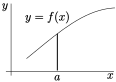
\includegraphics[width=\linewidth]{external/text/figs/areaAA.pdf}
\end{sbspanel}%
\begin{sbspanel}{0.5}[center]%
\includegraphics[width=\linewidth]{external/text/figs/areaABC.pdf}
\end{sbspanel}%
\end{sidebyside}%
\par
Note that we have assumed that \(a\leq c \leq b\) and that \(f(x)\geq 0\). One can  remove  these restrictions and also make the proof more formal, but it becomes quite  tedious and   less intuitive.%
\end{itemize}
%
\end{proof}
\begin{remark}{Remark}{}{remark-sec_def_int-b-k}%
For notational simplicity, let's assume that \(a\le c\le b\) and \(f(x)\ge 0\) for all \(a\le x\le b\).  The geometric interpretations of the identities%
\begin{gather*}
\int_a^a f(x)\dee{x}=0\quad\text{and}\quad
\int_a^b f(x)\dee{x}= \int_a^c f(x)\dee{x} + \int_c^b f(x)\dee{x}
\end{gather*}
are%
\begin{gather*}
\text{Area}\big\{\ (x,y)\ \big|\ a\le x\le a,\ 0\le y\le f(x)\ \big\}=0
\end{gather*}
and%
\begin{align*}
&\text{Area}\big\{\ (x,y)\ \big|\ a\le x\le b,\ 0\le y\le f(x)\ \big\}\\
&\hskip0.25in=\text{Area}\big\{\ (x,y)\ \big|\ a\le x\le c,\ 0\le y\le f(x)\ \big\}\\
&\hskip0.5in
+\text{Area}\big\{\ (x,y)\ \big|\ c\le x\le b,\ 0\le y\le f(x)\ \big\}
\end{align*}
respectively. Both of these geometric statements are intuitively obvious. See the figures below. We won't give a formal proof.%
\begin{sidebyside}{2}{0.0275}{0.0275}{0.055}%
\begin{sbspanel}{0.29}[center]%
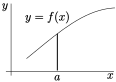
\includegraphics[width=\linewidth]{external/text/figs/areaAA.pdf}
\end{sbspanel}%
\begin{sbspanel}{0.6}[center]%
\includegraphics[width=\linewidth]{external/text/figs/areaABC.pdf}
\end{sbspanel}%
\end{sidebyside}%
\par
So we concentrate on the formula \(\int_b^a f(x)\dee{x}= -\int_a^b f(x)\dee{x}\). The midpoint Riemann sum approximation to \(\int_a^b f(x)\dee{x}\) with \(4\) subintervals (so that each subinterval has width \(\frac{b-a}{4}\)) is%
\begin{align}
&\Big\{f\big(a+\tfrac{1}{2}\tfrac{b-a}{4}\big)
+f\big(a+\tfrac{3}{2}\tfrac{b-a}{4}\big)
+f\big(a+\tfrac{5}{2}\tfrac{b-a}{4}\big)
+f\big(a+\tfrac{7}{2}\tfrac{b-a}{4}\big)\big\}\ \tfrac{b-a}{4}\notag\\
&=\Big\{f\big(\tfrac{7}{8}a+\tfrac{1}{8}b\big)
+f\big(\tfrac{5}{8}a+\tfrac{3}{8}b\Big)
+f\big(\tfrac{3}{8}a+\tfrac{5}{8}b\Big)
+f\big(\tfrac{1}{8}a+\tfrac{7}{8}b\big)\Big\}\ \tfrac{b-a}{4}\tag{\textasteriskcentered}\label{mrow-eq_INTflipL}
\end{align}
We're now going to write out the midpoint Riemann sum approximation to  \(\int_b^a f(x)\dee{x}\) with \(4\) subintervals. Note that \(b\) is now the lower limit on the integral and \(a\) is now the upper limit on the integral. This is likely to cause confusion when we write out the Riemann sum, so we'll temporarily rename \(b\) to \(A\) and \(a\) to \(B\). The midpoint Riemann sum approximation to \(\int_A^B f(x)\dee{x}\) with  \(4\) subintervals is%
\begin{align*}
&\Big\{f\big(A+\tfrac{1}{2}\tfrac{B-A}{4}\big)
+f\big(A+\tfrac{3}{2}\tfrac{B-A}{4}\big)
+f\big(A+\tfrac{5}{2}\tfrac{B-A}{4}\big)
+f\big(A+\tfrac{7}{2}\tfrac{B-A}{4}\big)\Big\}\ \tfrac{B-A}{4}\\
&=\Big\{f\big(\tfrac{7}{8}A+\tfrac{1}{8}B\big)
+f\big(\tfrac{5}{8}A+\tfrac{3}{8}B\big)
+f\big(\tfrac{3}{8}A+\tfrac{5}{8}B\big)
+f\big(\tfrac{1}{8}A+\tfrac{7}{8}B\big)\Big\}\ \tfrac{B-A}{4}
\end{align*}
Now recalling that \(A=b\) and \(B=a\), we have that the midpoint Riemann  sum approximation to \(\int_b^a f(x)\dee{x}\) with  \(4\) subintervals is%
\begin{gather}
\Big\{f\big(\frac{7}{8}b+\frac{1}{8}a\big)
+f\big(\tfrac{5}{8}b+\tfrac{3}{8}a\big)
+f\big(\tfrac{3}{8}b+\tfrac{5}{8}a\big)
+f\big(\tfrac{1}{8}b+\tfrac{7}{8}a\big)\Big\}\ \tfrac{a-b}{4}\tag{\textasteriskcentered\textasteriskcentered}\label{mrow-eq_INTflipR}
\end{gather}
The curly brackets in \hyperref[mrow-eq_INTflipL]{({\xreffont\ref{mrow-eq_INTflipL}})} and \hyperref[mrow-eq_INTflipR]{({\xreffont\ref{mrow-eq_INTflipR}})} are equal to each other \textemdash{} the terms are just in the reverse order. The factors multiplying the curly brackets in \hyperref[mrow-eq_INTflipL]{({\xreffont\ref{mrow-eq_INTflipL}})} and  \hyperref[mrow-eq_INTflipR]{({\xreffont\ref{mrow-eq_INTflipR}})}, namely \(\frac{b-a}{4}\) and \(\frac{a-b}{4}\), are negatives of each other, so  \hyperref[mrow-eq_INTflipR]{({\xreffont\ref{mrow-eq_INTflipR}})}\(=-\)\hyperref[mrow-eq_INTflipL]{({\xreffont\ref{mrow-eq_INTflipL}})}. The same computation with \(n\) subintervals shows that the midpoint Riemann sum approximations to  \(\int_b^a f(x)\dee{x}\) and \(\int_a^b f(x)\dee{x}\) with \(n\) subintervals are negatives of each other. Taking the limit \(n\rightarrow\infty\) gives \(\int_b^a f(x)\dee{x}= -\int_a^b f(x)\dee{x}\).%
\end{remark}
\begin{example}{Example}{Revisiting Example {\xreffont\ref*{example-eg_INTtriangle}}.}{example-eg_INTPROPxa}%
Back in Example~\hyperref[example-eg_INTtriangle]{{\xreffont\ref{example-eg_INTtriangle}}} we saw that when \(b \gt 0\) \(\int_0^b x\dee{x} =\frac{b^2}{2}\). We'll now verify that  \(\int_0^b x\dee{x} =\frac{b^2}{2}\) is still true when \(b=0\) and also when \(b \lt 0\).%
\begin{itemize}[label=\textbullet]
\item{}First consider \(b=0\). Then the statement \(\int_0^b x\dee{x} =\frac{b^2}{2}\) becomes%
\begin{gather*}
\int_0^0 x\dee{x} =0
\end{gather*}
This is an immediate consequence of Theorem \hyperref[theorem-thm_Intdomain]{{\xreffont\ref{theorem-thm_Intdomain}}}(a).%
\item{}Now consider \(b \lt 0\). Let us write \(B=-b\), so that \(B \gt 0\). In  Example~\hyperref[example-eg_INTtriangle]{{\xreffont\ref{example-eg_INTtriangle}}} we saw that%
\begin{gather*}
\int_{-B}^0 x\dee{x} =-\frac{B^2}{2}.
\end{gather*}
So we have%
\begin{align*}
\int_0^b x\dee{x}
&=\int^{-B}_0 x\dee{x} =- \int_{-B}^0 x\dee{x} & \text{by Theorem }\hyperref[theorem-thm_Intdomain]{\text{{\xreffont\ref{theorem-thm_Intdomain}}}}\text{(b)}\\
& =-\left(-\frac{B^2}{2}\right) & \text{by Example }\hyperref[example-eg_INTtriangle]{\text{{\xreffont\ref{example-eg_INTtriangle}}}}\\
& =\frac{B^2}{2} = \frac{b^2}{2}
\end{align*}
%
\end{itemize}
We have now shown that%
\begin{align*}
\int_0^b x\dee{x} &=\frac{b^2}{2} &\text{ for all real numbers $b$}
\end{align*}
%
\end{example}
\begin{example}{Example}{\(\int_a^b x\dee{x}\).}{example-eg_INTPROPx}%
Applying Theorem \hyperref[theorem-thm_Intdomain]{{\xreffont\ref{theorem-thm_Intdomain}}} yet again, we have, for all real numbers \(a\) and \(b\),%
\begin{align*}
\int_a^b x\dee{x} &=  \int_a^0 x\dee{x} + \int_0^b x\dee{x} &
\text{by Theorem }\hyperref[theorem-thm_Intdomain]{\text{{\xreffont\ref{theorem-thm_Intdomain}}}}(c)\text{ with $c=0$}\\
&=  \int_0^b x\dee{x} - \int_0^a x\dee{x} &
\text{by Theorem }\hyperref[theorem-thm_Intdomain]{\text{{\xreffont\ref{theorem-thm_Intdomain}}}}\text{(b)}\\
&=\frac{b^2-a^2}{2} &
\text{by Example }\hyperref[example-eg_INTPROPxa]{\text{{\xreffont\ref{example-eg_INTPROPxa}}}}\text{, twice}
\end{align*}
We can also understand this result geometrically.%
\begin{sidebyside}{1}{0.1}{0.1}{0}%
\begin{sbspanel}{0.8}%
\includegraphics[width=\linewidth]{external/text/figs/triangles_adr.pdf}
\end{sbspanel}%
\end{sidebyside}%
\par
%
\begin{itemize}[label=\textbullet]
\item{}(left) When \(0 \lt a \lt b\), the integral represents the area in green which  is the difference of two right-angle triangles \textemdash{} the larger with area \(b^2/2\)  and the smaller with area \(a^2/2\).%
\item{}(centre) When \(a \lt 0 \lt b\), the integral represents the signed area of the two  displayed triangles. The one above the axis has area \(b^2/2\) while the one  below has area \(-a^2/2\) (since it is below the axis).%
\item{}(right) When \(a \lt b \lt 0\), the integral represents the signed area in purple  of the difference between the two triangles \textemdash{} the larger with area \(-a^2/2\)  and the smaller with area \(-b^2/2\).%
\end{itemize}
%
\end{example}
Theorem~\hyperref[theorem-thm_Intdomain]{{\xreffont\ref{theorem-thm_Intdomain}}}(c) shows us how we can split an integral over a  larger interval into one over two (or more) smaller intervals. This is  particularly useful for dealing with piece-wise functions, like \(|x|\).%
\begin{example}{Example}{Integrals involving \(|x|\).}{example-eg_INTPROPabs}%
Using Theorem~\hyperref[theorem-thm_Intdomain]{{\xreffont\ref{theorem-thm_Intdomain}}}, we can readily evaluate integrals involving  \(|x|\). First, recall that%
\begin{align*}
|x|=\begin{cases}
x & \text{if $x\ge 0$} \\
-x & \text{if $x \lt  0$}
\end{cases}
\end{align*}
Now consider (for example) \(\int_{-2}^3 |x| \dee{x}\). Since the integrand  changes at \(x=0\), it makes sense to split the interval of integration at that  point:%
\begin{align*}
\int_{-2}^3 |x| \dee{x}
&= \int_{-2}^0 |x| \dee{x} + \int_0^3 |x| \dee{x}
&\text{by Theorem }\hyperref[theorem-thm_Intdomain]{\text{{\xreffont\ref{theorem-thm_Intdomain}}}}\\
&= \int_{-2}^0 (-x) \dee{x} + \int_0^3 x \dee{x}
&\text{by definition of $|x|$}\\
&= -\int_{-2}^0 x\dee{x} + \int_0^3 x \dee{x}
&\text{by Theorem }\hyperref[theorem-thm_Intarith]{\text{{\xreffont\ref{theorem-thm_Intarith}}}}\text{(c)}\\
&= - (-2^2/2) + (3^2/2) = (4+9)/2\\
&= 13/2
\end{align*}
We can go further still \textemdash{} given a function \(f(x)\) we can rewrite  the integral of \(f(|x|)\) in terms of the integral of \(f(x)\) and \(f(-x)\).%
\begin{align*}
\int_{-1}^1 f\big(|x|\big)\dee{x} & = \int_{-1}^0 f\big(|x|\big)\dee{x}+ \int_0^1 f\big(|x|\big)\dee{x}\\
& = \int_{-1}^0 f(-x)\dee{x}+ \int_0^1 f(x)\dee{x}
\end{align*}
%
\end{example}
Here is a more concrete example.%
\begin{example}{Example}{Revisiting Example {\xreffont\ref*{example-eg_INTtriangleB}}.}{example-sec_def_int-b-q}%
Let us compute \(\int_{-1}^1 \big(1-|x|\big)\dee{x}\) again. In  Example~\hyperref[example-eg_INTtriangleB]{{\xreffont\ref{example-eg_INTtriangleB}}} we evaluated this integral by interpreting it as  the area of a triangle. This time we are going to use \emph{only} the  properties given in Theorems~\hyperref[theorem-thm_Intarith]{{\xreffont\ref{theorem-thm_Intarith}}} and~\hyperref[theorem-thm_Intdomain]{{\xreffont\ref{theorem-thm_Intdomain}}} and the  facts that%
\begin{align*}
\int_a^b \dee{x} &= b-a &\text{and}&&
\int_a^b x\dee{x}=\frac{b^2-a^2}{2}
\end{align*}
That \(\int_a^b\dee{x} = b-a\) is part (e) of Theorem~\hyperref[theorem-thm_Intarith]{{\xreffont\ref{theorem-thm_Intarith}}}. We saw that \(\int_a^b x\dee{x}=\frac{b^2-a^2}{2}\) in Example~\hyperref[example-eg_INTPROPx]{{\xreffont\ref{example-eg_INTPROPx}}}.%
\par
First we are going to get rid of the absolute value signs by splitting the  interval over which we integrate. Recalling that \(|x|=x\) whenever \(x\ge 0\) and  \(|x|=-x\) whenever \(x\le 0\), we split the interval by  Theorem~\hyperref[theorem-thm_Intdomain]{{\xreffont\ref{theorem-thm_Intdomain}}}(c),%
\begin{align*}
\int_{-1}^1 \big(1-|x|\big)\dee{x} &=\int_{-1}^0 \big(1-|x|\big)\dee{x} + \int_0^1 \big(1-|x|\big)\dee{x}\\
&=\int_{-1}^0 \big(1-(-x)\big)\dee{x} + \int_0^1 \big(1-x\big)\dee{x}\\
&=\int_{-1}^0 \big(1+x\big)\dee{x} + \int_0^1 \big(1-x\big)\dee{x}
\end{align*}
Now we apply parts (a) and (b) of Theorem \hyperref[theorem-thm_Intarith]{{\xreffont\ref{theorem-thm_Intarith}}}, and then%
\begin{align*}
\int_{-1}^1 \big[1-|x|\big]\dee{x}
&=\int_{-1}^0 1\dee{x} + \int_{-1}^0 x\dee{x} + \int_0^1 1\dee{x}  - \int_0^1 x\dee{x}\\
&=[0-(-1)]+\frac{0^2-(-1)^2}{2}+[1-0]-\frac{1^2-0^2}{2}\\
&=1
\end{align*}
%
\end{example}
\end{introduction}%
%
%
\typeout{************************************************}
\typeout{Subsection 1.2.1 More properties of integration: even and odd functions}
\typeout{************************************************}
%
\begin{subsectionptx}{Subsection}{More properties of integration: even and odd functions}{}{More properties of integration: even and odd functions}{}{}{subsection-sec_evenodd}
Recall \footnote{We haven't done this in this course, but you should have seen  it in your differential calculus course or perhaps even earlier.\label{fn-sec_evenodd-b-a}} the following definition%
\begin{definition}{Definition}{}{definition-def_INTevenodd}%
Let \(f(x)\) be a function. Then,%
\begin{itemize}[label=\textbullet]
\item{}we say that \(f(x)\) is even when \(f(x)=f(-x)\) for all \(x\), and%
\item{}we say that \(f(x)\) is odd when \(f(x)=-f(-x)\) for all \(x\).%
\end{itemize}
%
\end{definition}
Of course most functions are neither even nor odd, but many of the standard  functions you know are.%
\begin{example}{Example}{Even functions.}{example-eg_lefthalfevenfunction}%
%
\begin{itemize}[label=\textbullet]
\item{}Three examples of even functions are \(f(x)=|x|\), \(f(x)=\cos x\) and  \(f(x)=x^2\). In fact, if \(f(x)\) is any even power of \(x\), then \(f(x)\) is an  even function.%
\item{}The part of the graph \(y=f(x)\) with \(x\le 0\), may be constructed by  drawing the part of the graph with \(x\ge 0\) (as in the figure on the left below) and then reflecting it in the \(y\)-axis (as in the figure on the right below).%
\begin{sidebyside}{2}{0.05}{0.05}{0.1}%
\begin{sbspanel}{0.4}[center]%
\includegraphics[width=\linewidth]{external/text/figs/evenCosPt.pdf}
\end{sbspanel}%
\begin{sbspanel}{0.4}[center]%
\includegraphics[width=\linewidth]{external/text/figs/evenCos.pdf}
\end{sbspanel}%
\end{sidebyside}%
\item{}In particular, if \(f(x)\) is an even function and \(a \gt 0\), then  the two sets%
\begin{align*}
&\big\{\ (x,y)\ \big|\
\text{$0\le x\le a$ and $y$ is between $0$ and $f(x)$} \ \big\}\\
&\big\{\ (x,y)\ \big|\
\text{$-a\le x\le 0$ and $y$ is between $0$ and $f(x)$} \ \big\}
\end{align*}
are reflections of each other in the \(y\)-axis and so have the same  signed area. That is%
\begin{align*}
\int_0^a f(x)\dee{x} &= \int_{-a}^0 f(x)\dee{x}
\end{align*}
%
\end{itemize}
%
\end{example}
\begin{example}{Example}{Odd functions.}{example-eg_areaunderoddfunction}%
%
\begin{itemize}[label=\textbullet]
\item{}Three examples of odd functions are \(f(x)=\sin x\), \(f(x)=\tan x\) and  \(f(x)=x^3\). In fact, if \(f(x)\) is any odd power of \(x\), then \(f(x)\) is  an odd function.%
\item{}The part of the graph \(y=f(x)\) with \(x\le 0\), may be constructed by  drawing the part of the graph with \(x\ge 0\) (like the solid line in the figure  on the left below) and then reflecting it in the \(y\)-axis (like the dashed  line  in the figure on the left below) and then reflecting the result in the \(x\)-axis  (i.e. flipping it upside down, like in the figure on the right, below).%
\begin{sidebyside}{2}{0.05}{0.05}{0.1}%
\begin{sbspanel}{0.4}[center]%
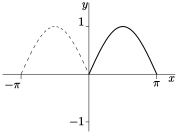
\includegraphics[width=\linewidth]{external/text/figs/oddSinPt.pdf}
\end{sbspanel}%
\begin{sbspanel}{0.4}[center]%
\includegraphics[width=\linewidth]{external/text/figs/oddSin.pdf}
\end{sbspanel}%
\end{sidebyside}%
\item{}In particular, if \(f(x)\) is an odd function and \(a \gt 0\), then the  signed areas of the two sets%
\begin{align*}
&\big\{\ (x,y)\ \big|\
\text{$0\le x\le a$ and $y$ is between $0$ and $f(x)$} \ \big\}\\
&\big\{\ (x,y)\ \big|\
\text{$-a\le x\le 0$ and $y$ is between $0$ and $f(x)$} \ \big\}
\end{align*}
are negatives of each other \textemdash{} to get from the first set to the second  set, you flip it upside down, in addition to reflecting it in the \(y\)-axis.  That is%
\begin{gather*}
\int_0^a f(x)\dee{x} = -\int_{-a}^0 f(x)\dee{x}
\end{gather*}
%
\end{itemize}
%
\end{example}
We can exploit the symmetries noted in the examples above, namely%
\begin{align*}
\int_0^a f(x)\dee{x} &= \int_{-a}^0 f(x)\dee{x} & \text{for $f$ even}\\
\int_0^a f(x)\dee{x} &= -\int_{-a}^0 f(x)\dee{x} & \text{for $f$ odd}
\end{align*}
together with Theorem~\hyperref[theorem-thm_Intdomain]{{\xreffont\ref{theorem-thm_Intdomain}}} Theorem \hyperref[theorem-thm_Intdomain]{{\xreffont\ref{theorem-thm_Intdomain}}}%
\begin{align*}
\int_{-a}^a f(x)\dee{x} &= \int_{-a}^0 f(x)\dee{x} + \int_0^a f(x) \dee{x}
\end{align*}
in order to simplify the integration of even and odd functions over intervals  of the form \([-a,a]\).%
\begin{theorem}{Theorem}{Even and Odd.}{}{theorem-thm_INTevenodd}%
Let \(a \gt 0\).%
\begin{enumerate}[label=\alph*]
\item{}If \(f(x)\) is an even function, then%
\begin{gather*}
\int_{-a}^a f(x) \dee{x} = 2\int_0^a f(x) \dee{x}
\end{gather*}
%
\item{}If \(f(x)\) is an odd function, then%
\begin{gather*}
\int_{-a}^a f(x) \dee{x} = 0
\end{gather*}
%
\end{enumerate}
%
\end{theorem}
\begin{proof}{Proof}{}{proof-sec_evenodd-i}
For any function%
\begin{gather*}
\int_{-a}^a f(x)\dee{x} = \int_0^a f(x)\dee{x} + \int_{-a}^0 f(x)\dee{x}
\end{gather*}
When \(f\) is even, the two terms on the right hand side are equal. When \(f\) is odd, the two terms on the right hand side are negatives of each other.%
\end{proof}
\end{subsectionptx}
%
%
\typeout{************************************************}
\typeout{Subsection 1.2.2 Optional \textemdash{} More properties of integration: inequalities for integrals}
\typeout{************************************************}
%
\begin{subsectionptx}{Subsection}{Optional \textemdash{} More properties of integration: inequalities for integrals}{}{Optional \textemdash{} More properties of integration: inequalities for integrals}{}{}{subsection-sec_def_int-d}
We are still unable to integrate many functions, however with a little work we  can infer bounds on integrals from bounds on their integrands.%
\begin{theorem}{Theorem}{Inequalities for Integrals.}{}{theorem-thm_INTineq}%
Let \(a\le b\)  be real numbers and let the functions \(f(x)\) and \(g(x)\) be integrable on the interval \(a\le x\le b\).%
\begin{enumerate}[label=\alph*]
\item{}If \(f(x)\ge 0\) for all \(a\le x\le b\), then%
\begin{gather*}
\int_a^b f(x)\,\dee{x} \ge 0
\end{gather*}
%
\item{}If \(f(x)\le g(x)\) for all \(a\le x\le b\), then%
\begin{gather*}
\int_a^b f(x)\,\dee{x} \le \int_a^b g(x)\,\dee{x}
\end{gather*}
%
\item{}If there are constants \(m\) and \(M\) such that  \(m\le f(x)\le M\)  for all \(a\le x\le b\), then%
\begin{gather*}
m(b-a)\le \int_a^b f(x)\,\dee{x} \le M(b-a)
\end{gather*}
%
\item{}We have%
\begin{gather*}
\bigg|\int_a^b f(x)\,\dee{x}\bigg|\le \int_a^b |f(x)|\,\dee{x}
\end{gather*}
%
\end{enumerate}
%
\end{theorem}
\begin{proof}{Proof}{}{proof-sec_def_int-d-d}
%
\begin{enumerate}[label=\alph*]
\item{}By interpreting the integral as the signed area, this statement  simply says that if the curve \(y=f(x)\) lies above the \(x\)-axis and \(a\le b\), then the signed area of  \(\big\{\ (x,y)\ \big|\ a\le x\le b,\   0\le y\le f(x)\ \big\}\) is at least zero. This is quite clear. Alternatively, we could argue more  algebraically from Definition~\hyperref[definition-def_INTintegral]{{\xreffont\ref{definition-def_INTintegral}}}. We observe that when we  define \(\int_a^b f(x)\dee{x}\) via Riemann sums, every  summand, \(f(x_{i,n}^*)\,\frac{b-a}{n}\ge 0\). Thus the whole sum is nonnegative  and consequently, so is the limit, and thus so is the integral.%
\item{}We are assuming that \(g(x)-f(x)\geq 0\), so part (a) gives%
\begin{align*}
\int_a^b\big[g(x)-f(x)\big]\,\dee{x}\ge 0
\amp\implies \int_a^b g(x)\,\dee{x}-\int_a^b f(x)\,\dee{x}\ge 0 \\
\amp\implies \int_a^b f(x)\,\dee{x} \le \int_a^b g(x)\,\dee{x}
\end{align*}
%
\item{}Applying part (b) with \(g(x)=M\) for all \(a\le x\le b\) gives%
\begin{gather*}
\int_a^b f(x)\,\dee{x} \le \int_a^b M\,\dee{x} = M(b-a)
\end{gather*}
Similarly, viewing \(m\) as a (constant) function, and applying part (b) gives%
\begin{gather*}
m\le f(x) \implies \overbrace{\int_a^bm\,\dee{x}}^{=m(b-a)} \le \int_a^b f(x)\,\dee{x}
\end{gather*}
%
\item{}For any \(x\), \(|f(x)|\) is either \(f(x)\) or \(-f(x)\) (depending on whether  \(f(x)\) is positive or negative), so we certainly have%
\begin{align*}
f(x)&\le |f(x)| & \text{and}&& -f(x)&\le |f(x)|
\end{align*}
Applying part (c) to each of those inequalities gives%
\begin{align*}
\int_a^b f(x)\dee{x} &\le \int_a^b |f(x)|\dee{x} & \text{and} &&
-\int_a^b f(x)\dee{x} &\le \int_a^b |f(x)|\dee{x}
\end{align*}
Now \(\Big|\int_a^b f(x)\dee{x}\Big|\) is either equal to \(\int_a^b f(x)\dee{x}\) or  \(-\int_a^b f(x)\dee{x}\) (depending on whether the integral is positive or  negative). In either case we can apply the above two inequalities to get the  same result, namely%
\begin{align*}
\left|\int_a^b f(x)\dee{x}\right| &\leq \int_a^b |f(x)|\dee{x}.
\end{align*}
%
\end{enumerate}
%
\end{proof}
\begin{example}{Example}{\(\int_0^{\frac{\pi}{3}}\sqrt{\cos x}\dee{x}\).}{example-sec_def_int-d-e}%
Consider the integral%
\begin{gather*}
\int_0^{\frac{\pi}{3}}\sqrt{\cos x}\dee{x}
\end{gather*}
This is not so easy to compute exactly \footnotemark{}, but we can bound it quite quickly.%
\par
For \(x\) between \(0\) and \(\frac{\pi}{3}\), the function \(\cos x\) takes  values \footnotemark{} between \(1\) and \(\frac{1}{2}\). Thus the function \(\sqrt{\cos x}\) takes values between \(1\) and \(\frac{1}{\sqrt{2}}\). That is%
\begin{align*}
\frac{1}{\sqrt{2}} &\le \sqrt{\cos x} \le 1 & \text{for $0\le x\le \frac{\pi}{3}$}.
\end{align*}
Consequently, by Theorem \hyperref[theorem-thm_INTineq]{{\xreffont\ref{theorem-thm_INTineq}}}(b) with  \(a=0\), \(b=\frac{\pi}{3}\), \(m= \frac{1}{\sqrt{2}}\) and \(M=1\),%
\begin{align*}
\frac{\pi}{3\sqrt{2}} &\le \int_0^{\frac{\pi}{3}} \sqrt{\cos x}\dee{x}  \le \frac{\pi}{3}\\
\\
\intertext{Plugging these expressions into a calculator gives us}
0.7404804898 & \le \int_0^{\frac{\pi}{3}} \sqrt{\cos x}\dee{x}  \leq 1.047197551
\end{align*}
%
\end{example}
\footnotetext[3]{It is not too hard to use Riemann sums and a computer to evaluate it numerically: \(0.948025319\dots\).\label{fn-sec_def_int-d-e-b-b}}%
\footnotetext[4]{You know the graphs of sine and cosine, so you should be able to work this out without too much difficulty.\label{fn-sec_def_int-d-e-c-e}}%
\end{subsectionptx}
%
%
\typeout{************************************************}
\typeout{Exercises 1.2.3 Exercises}
\typeout{************************************************}
%
\begin{exercises-subsection}{Exercises}{Exercises}{}{Exercises}{}{}{exercises-sec_def_int-e}
\par\medskip\noindent%
\textbf{.}\space\space%
\begin{exercisegroup}
\begin{divisionexerciseeg}{1}{}{}{exercise-sec_def_int-e-a-c}%
For each of the following properties of definite integrals, draw a picture illustrating the concept, interpreting definite integrals as areas under a curve.%
\par
For simplicity, you may assume that \(a \leq c \leq b\), and that \(f(x),g(x)\) give positive values.%
\begin{enumerate}[label=\alph*]
\item{}\(\displaystyle\int_a^a f(x)\,\dee{x}=0\), (Theorem~\hyperref[theorem-thm_Intdomain]{{\xreffont\ref{theorem-thm_Intdomain}}}, part (a))%
\item{}\(\displaystyle\int_a^b f(x)\,\dee{x}= \displaystyle\int_a^c f(x)\,\dee{x} + \int_c^b f(x)\dee{x} \), (Theorem~\hyperref[theorem-thm_Intdomain]{{\xreffont\ref{theorem-thm_Intdomain}}}, part (c))%
\item{}\(\displaystyle\int_a^b \left( f(x) + g(x) \right)\,\dee{x}
= \displaystyle\int_a^b f(x)\,\dee{x} + \displaystyle\int_a^b g(x)\,\dee{x}\), (Theorem~\hyperref[theorem-thm_Intarith]{{\xreffont\ref{theorem-thm_Intarith}}}, part (a))%
\end{enumerate}
%
\end{divisionexerciseeg}%
\begin{divisionexerciseeg}{2}{}{}{exercise-sec_def_int-e-a-d}%
If \(\displaystyle\int_0^b \cos x\dee{x}=\sin b\), then what is \(\displaystyle\int_a^b \cos x\dee{x}\)?%
\end{divisionexerciseeg}%
\begin{divisionexerciseeg}{3}{2015A, 2016A.}{}{exercise-sec_def_int-e-a-e}%
Decide whether each of the following statements is true or false. If false, provide a counterexample. If true, provide a brief justification. (Assume that \(f(x)\) and \(g(x)\) are continuous functions.)%
\par
%
\begin{enumerate}[label=\alph*]
\item{}\(\displaystyle\int_{-3}^{-2} f(x) \dee{x}=-\displaystyle\int_{3}^{2} f(x) \dee{x}\).%
\item{}If \(f(x)\) is an odd function, then \(\displaystyle \int_{-3}^{-2} f(x)\,\dee{x} = \int_2^3 f(x)\,\dee{x}\).%
\item{}\(\displaystyle\int_{0}^{1} f(x)\cdot g(x) \dee{x} =\int_{0}^{1} f(x) \dee{x} \cdot \int_{0}^{1} g(x)\dee{x}\).%
\end{enumerate}
%
\end{divisionexerciseeg}%
\begin{divisionexerciseeg}{4}{}{}{exercise-sec_def_int-e-a-f}%
Suppose we want to make a right Riemann sum with 100 intervals to approximate \(\int\limits_5^0 f(x)\dee{x}\), where \(f(x)\) is a function that gives only positive values.%
\begin{enumerate}[label=\alph*]
\item{}What is \(\Delta x\)?%
\item{}Are the heights of our rectangles positive or negative?%
\item{}Is our Riemann sum positive or negative?%
\item{}Is the signed area under the curve \(y=f(x)\) from \(x=0\) to \(x=5\) positive or negative?%
\end{enumerate}
%
\end{divisionexerciseeg}%
\end{exercisegroup}
\par\medskip\noindent
\par\medskip\noindent%
\textbf{.}\space\space%
\begin{exercisegroup}
\begin{divisionexerciseeg}{5}{M105 2015A.}{}{exercise-sec_def_int-e-b-c}%
Suppose \(\displaystyle\int_2^3 f(x)\,\dee{x} = -1\) and \(\displaystyle\int_2^3 g(x)\,\dee{x} = 5\). Evaluate \(\displaystyle \int_2^3 \big( 6 f(x) - 3 g(x) \big)\,\dee{x}\).%
\end{divisionexerciseeg}%
\begin{divisionexerciseeg}{6}{2016Q1.}{}{exercise-sec_def_int-e-b-d}%
If \(\displaystyle\int_0^2 f(x)\,\dee{x} = 3\) and \(\displaystyle\int_0^2 g(x)\,\dee{x} = -4\), calculate \(\displaystyle \int_0^2 \big( 2 f(x) + 3 g(x) \big)\,\dee{x}\).%
\end{divisionexerciseeg}%
\begin{divisionexerciseeg}{7}{2016Q1.}{}{exercise-sec_def_int-e-b-e}%
The functions \(f(x)\) and \(g(x)\) obey%
\begin{align*}
\int_0^{-1} f(x)\,\dee{x} &= 1 &
\int_0^2 f(x)\,\dee{x} &= 2 \\
\int_{-1}^0 g(x)\,\dee{x} &= 3 &
\int_0^2 g(x)\,\dee{x} &= 4
\end{align*}
Find \(\int_{-1}^2 \big[3g(x)-f(x)\big]\,\dee{x}\).%
\end{divisionexerciseeg}%
\begin{divisionexerciseeg}{8}{}{}{exercise-sec_def_int-e-b-f}%
In Question~\hyperlink{exercise-p1_1_awkwardcircle}{{\xreffont 1.1.8.45}}, Section~\hyperref[section-sec_intdef]{{\xreffont\ref{section-sec_intdef}}}, we found that%
\begin{equation*}
\int_0^a\sqrt{1-x^2}\dee{x}=\frac{\pi}{4} - \frac{1}{2}\arccos(a)+\frac{1}{2}a\sqrt{1-a^2}
\end{equation*}
%
\par
when \(0\le a\le 1\).%
\par
Using this fact, evaluate the following:%
\begin{enumerate}[label=\alph*]
\item{}\(\displaystyle\int_{a}^0 \sqrt{1-x^2}\dee{x}\), where \(-1 \leq a \leq 0\)%
\item{}\(\displaystyle\int_{a}^1 \sqrt{1-x^2}\dee{x}\), where \(0 \leq a \leq 1\)%
\end{enumerate}
%
\end{divisionexerciseeg}%
\begin{divisionexerciseeg}{9}{M105 2013A.}{}{exercise-prob_s1_2_2}%
Evaluate \({\displaystyle\int_{-1}^2 |2x|\dee{x}}\).%
\par
You may use the result from  Example \hyperref[example-eg_INTPROPx]{{\xreffont\ref{example-eg_INTPROPx}}} that \(\int\limits_a^b x\dee{x}=\frac{b^2-a^2}{2}\).%
\end{divisionexerciseeg}%
\begin{divisionexerciseeg}{10}{}{}{exercise-sec_def_int-e-b-h}%
Evaluate \(\displaystyle\int_{-5}^5 x|x|\dee{x}\,.\)%
\end{divisionexerciseeg}%
\begin{divisionexerciseeg}{11}{}{}{exercise-sec_def_int-e-b-i}%
Suppose \(f(x)\) is an even function and \(\displaystyle\int_{-2}^2 f(x)\dee{x}=10\). What is \(\displaystyle\int_{-2}^0 f(x)\dee{x}\)?%
\end{divisionexerciseeg}%
\end{exercisegroup}
\par\medskip\noindent
\par\medskip\noindent%
\textbf{.}\space\space%
\begin{exercisegroup}
\begin{divisionexerciseeg}{12}{2016Q1.}{}{exercise-sec_def_int-e-c-c}%
Evaluate \(\displaystyle\int_{-2}^{2} \left(5+\sqrt{4-x^2}\right)\dee{x}\).%
\end{divisionexerciseeg}%
\begin{divisionexerciseeg}{13}{M121 2012A.}{}{exercise-sec_def_int-e-c-d}%
Evaluate \(\displaystyle\int_{-2012}^{+2012} \frac{\sin x}{\log(3+x^2)}\dee{x}\).%
\end{divisionexerciseeg}%
\begin{divisionexerciseeg}{14}{2012A.}{}{exercise-sec_def_int-e-c-e}%
Evaluate \(\displaystyle\int_{-2012}^{+2012} x^{1/3}\cos x\,\dee{x}\).%
\end{divisionexerciseeg}%
\begin{divisionexerciseeg}{15}{}{}{exercise-sec_def_int-e-c-f}%
Evaluate \(\displaystyle\int_{0}^6 (x-3)^3\,\dee{x}\,.\)%
\end{divisionexerciseeg}%
\begin{divisionexerciseeg}{16}{}{}{exercise-prob_s1_2_ellipsearea}%
We want to compute the area of an ellipse, \((ax)^2+(by)^2=1\) for some (let's say positive) constants \(a\) and \(b\).%
\begin{enumerate}[label=\alph*]
\item{}Solve the equation for the upper half of the ellipse. It should have the form ``\(y=\cdots\)''%
\item{}Write an integral for the area of the upper half of the ellipse. Using properties of integrals, make the integrand look like the upper half of a circle.%
\item{}Using geometry and your answer to part (b), find the area of the ellipse.%
\end{enumerate}
%
\end{divisionexerciseeg}%
\begin{divisionexerciseeg}{17}{}{}{exercise-sec_def_int-e-c-h}%
Fill in the following table: the product of an (even\slash{}odd) function with an (even\slash{}odd) function is an (even\slash{}odd) function. You may assume that both functions are defined for all real numbers.%
\begin{sidebyside}{1}{0}{0}{0}%
\begin{sbspanel}{1}%
\resizebox{\ifdim\width > \linewidth\linewidth\else\width\fi}{!}{%
{\centering%
{\tabularfont%
\begin{tabular}{AlAlAlA}\hrulethin
\(\times\)&even&odd\tabularnewline\hrulethin
even&&\tabularnewline\hrulethin
odd&&\tabularnewline\hrulethin
\end{tabular}
}%
\par}
}%
\end{sbspanel}%
\end{sidebyside}%
\end{divisionexerciseeg}%
\begin{divisionexerciseeg}{18}{}{}{exercise-sec_def_int-e-c-i}%
Suppose \(f(x)\) is an odd function and \(g(x)\) is an even function, both defined at \(x=0\). What are the possible values of \(f(0)\) and \(g(0)\)?%
\end{divisionexerciseeg}%
\begin{divisionexerciseeg}{19}{}{}{exercise-p1_1_bothevenodd}%
Suppose \(f(x)\) is a function defined on all real numbers that is both even and odd. What could \(f(x)\) be?%
\end{divisionexerciseeg}%
\begin{divisionexerciseeg}{20}{}{}{exercise-p1_2_derivevenodd}%
Is the derivative of an even function even or odd? Is the derivative of an odd function even or odd?%
\end{divisionexerciseeg}%
\end{exercisegroup}
\par\medskip\noindent
\end{exercises-subsection}
\end{sectionptx}
%
%
\typeout{************************************************}
\typeout{Section 1.3 The Fundamental Theorem of Calculus}
\typeout{************************************************}
%
\begin{sectionptx}{Section}{The Fundamental Theorem of Calculus}{}{The Fundamental Theorem of Calculus}{}{}{section-sec_fundamental}
\begin{introduction}{}%
\end{introduction}%
%
%
\typeout{************************************************}
\typeout{Subsection 1.3.1 The Fundamental Theorem of Calculus}
\typeout{************************************************}
%
\begin{subsectionptx}{Subsection}{The Fundamental Theorem of Calculus}{}{The Fundamental Theorem of Calculus}{}{}{subsection-sec_fundamental-c}
We have spent quite a few pages (and lectures) talking about definite  integrals, what they are (Definition~\hyperref[definition-def_INTintegral]{{\xreffont\ref{definition-def_INTintegral}}}), when they  exist (Theorem~\hyperref[theorem-thm_integrable]{{\xreffont\ref{theorem-thm_integrable}}}), how to compute some special  cases (Section~\hyperref[subsection-ssec_knownareas]{{\xreffont\ref{subsection-ssec_knownareas}}}), some ways to manipulate them  (Theorem~\hyperref[theorem-thm_Intarith]{{\xreffont\ref{theorem-thm_Intarith}}} and~\hyperref[theorem-thm_Intdomain]{{\xreffont\ref{theorem-thm_Intdomain}}}) and how to bound them  (Theorem~\hyperref[theorem-thm_INTineq]{{\xreffont\ref{theorem-thm_INTineq}}}). Conspicuously missing from all of this has been a  discussion of how to compute them in general. It is high time we rectified  that.%
\par
The single most important tool used to evaluate integrals is called ``the fundamental theorem of calculus''. Its grand name is justified \textemdash{} it  links the two branches of calculus by connecting derivatives to integrals. In  so  doing it also tells us how to compute integrals. Very roughly speaking the  derivative of an integral is the original function. This fact allows us to  compute integrals using antiderivatives \footnote{You learned these near the  end of your differential calculus course. Now is a good time to revise \textemdash{}  but we'll go over them here since they are so important in what follows.\label{fn-sec_fundamental-c-c-c}}. Of course ``very rough'' is not enough \textemdash{} let's be precise.%
\begin{theorem}{Theorem}{Fundamental Theorem of Calculus.}{}{theorem-thm_INTfundthmofcalc}%
Let \(a \lt b\) and let \(f(x)\) be a function which is defined and continuous on  \([a,b]\).%
\begin{itemize}[label=\textbullet]
\item{}\alert{Part 1}. Let \(\ds F(x)=\int_a^x f(t)\dee{t}\) for any \(x  \in[a,b]\). Then the function \(F(x)\) is differentiable and further%
\begin{align*}
F'(x) &=f(x)
\end{align*}
%
\item{}\alert{Part 2}. Let \(G(x)\) be any function which is defined and  continuous on \([a,b]\). Further let \(G(x)\) be differentiable with \(G'(x)=f(x)\)  for all \(a \lt x \lt b\). Then%
\begin{align*}
\int_a^b f(x)\dee{x} &=G(b)-G(a) & \text{or equivalently} &&
\int_a^b G'(x)\dee{x} &=G(b)-G(a)
\end{align*}
%
\end{itemize}
%
\end{theorem}
Before we prove this theorem and look at a bunch of examples of its  application, it is important that we recall one definition from differential  calculus \textemdash{} antiderivatives. If \(F'(x) = f(x)\) on some interval, then  \(F(x)\)  is called an antiderivative of \(f(x)\) on that interval. So Part 2 of the the  fundamental theorem of calculus tells us how to evaluate the definite integral  of \(f(x)\) in terms of any of its antiderivatives \textemdash{}  if  \(G(x)\) is any  antiderivative of \(f(x)\) then%
\begin{align*}
\int_a^b f(x) \dee x &= G(b)-G(a)
\end{align*}
The form \(\int_a^b G'(x)\,\dee{x} = G(b) - G(a)\) of the fundamental theorem relates the  rate of change of \(G(x)\) over the interval \(a\le x\le b\) to the net change of \(G\) between  \(x=a\) and \(x=b\). For that reason, it is sometimes called the ``net change theorem''.%
\par
We'll start with a simple example. Then we'll see why the  fundamental theorem is true and then we'll do many more, and more involved,  examples.%
\begin{example}{Example}{A first example.}{example-eg_first}%
Consider the integral \(\int_a^b x \dee{x}\) which we have explored previously  in Example~\hyperref[example-eg_INTPROPx]{{\xreffont\ref{example-eg_INTPROPx}}}.%
\begin{itemize}[label=\textbullet]
\item{}The integrand is \(f(x)=x\).%
\item{}We can readily verify that \(G(x) = \frac{x^2}{2}\) satisfies \(G'(x)=f(x)\)  and so is an antiderivative of the integrand.%
\item{}Part 2 of Theorem~\hyperref[theorem-thm_INTfundthmofcalc]{{\xreffont\ref{theorem-thm_INTfundthmofcalc}}} then tells us that%
\begin{align*}
\int_a^b f(x) \dee{x} &= G(b)-G(a)\\
\int_a^b x \dee{x} &= \frac{b^2}{2} - \frac{a^2}{2}
\end{align*}
which is precisely the result we obtained (with more work) in  Example~\hyperref[example-eg_INTPROPx]{{\xreffont\ref{example-eg_INTPROPx}}}.%
\end{itemize}
%
\end{example}
We do not give completely rigorous proofs of the two parts of the theorem \textemdash{}  that is not really needed for this course. We just give the main ideas of the  proofs so that you can understand why the theorem is true.%
\begin{proof}{Proof}{Part 1.}{proof-sec_fundamental-c-i}
We wish to show that if%
\begin{align*}
F(x) &= \int_a^x f(t) \dee{t} & \text{then}&&
F'(x) &= f(x)
\end{align*}
%
\begin{itemize}[label=\textbullet]
\item{}Assume that \(F\) is the above integral and then consider \(F'(x)\). By  definition%
\begin{align*}
F'(x) &=\lim_{h\rightarrow 0} \frac{F(x+h)-F(x)}{h}
\end{align*}
%
\item{}To understand this limit, we interpret the terms \(F(x), F(x+h)\) as signed  areas. To simplify this further, let's only consider the case that \(f\) is always nonnegative and that \(h \gt 0\). These restrictions are not hard to remove, but the  proof ideas are a bit cleaner if we keep them in place. Then we have%
\begin{align*}
F(x+h)&=\text{the area of the region $\big\{\ (t,y)\ \big|\ a\le t\le x+h,\
0\le y\le f(t)\ \big\}$}\\
F(x)&=\text{the area of the region $\big\{\ (t,y)\ \big|\ a\le t\le x,
\phantom{+h\ \,}\  0\le y\le f(t)\ \big\}$}
\end{align*}
%
\item{}Then the numerator%
\begin{gather*}
F(x+h)-F(x)=\text{the area of $\big\{\ (t,y)\ \big|\ x\le t\le x+h,\
0\le y\le f(t)\ \big\} $}
\end{gather*}
This is just the more darkly shaded region in the figure%
\begin{sidebyside}{1}{0.25}{0.25}{0}%
\begin{sbspanel}{0.5}%
\includegraphics[width=\linewidth]{external/text/figs/fundThm.pdf}
\end{sbspanel}%
\end{sidebyside}%
\item{}We will be taking the limit \(h\rightarrow 0\). So suppose that \(h\) is  very small. Then, as \(t\) runs from \(x\) to \(x+h\), \(f(t)\) runs only over  a very narrow range of values\footnote{Notice that if \(f\) were discontinuous, then this might be false.\label{fn-sec_fundamental-c-i-b-b-d-g}}, all close to \(f(x)\).%
\item{}So the darkly shaded region is almost a rectangle of width \(h\) and height  \(f(x)\) and so has an area which is very close to \(f(x)h\). Thus \(\frac{F(x+h)-F(x)}{h}\) is very close to \(f(x)\).%
\item{}In the limit \(h\rightarrow 0\), \(\frac{F(x+h)-F(x)}{h}\) becomes exactly \(f(x)\), which is precisely what we want.%
\end{itemize}
%
\end{proof}
We can make the above more rigorous using the Mean Value Theorem \footnote{The  MVT tells us that there is a number \(c\) between \(x\) and \(x+h\) so that \(F'(c) = \frac{F(x+h)-F(x)}{(x+h)-x} = \frac{F(x+h)-F(x)}{h}\). But since \(F'(x) = f(x)\), this tells us that \(\frac{F(x+h)-F(x)}{h} = f(c)\) where \(c\) is trapped between \(x+h\) and \(x\). Now when we take the limit as \(h \to 0\) we have that this number \(c\) is squeezed to \(x\) and the result follows.\label{fn-sec_fundamental-c-j-a}}.%
\begin{proof}{Proof}{Part 2.}{proof-sec_fundamental-c-k}
We want to show that \(\int_a^b f(t)\dee{t}=G(b)-G(a)\). To do this we exploit  the fact that the derivative of a constant is zero.%
\begin{itemize}[label=\textbullet]
\item{}Let%
\begin{align*}
H(x) &= \int_a^x f(t)\dee{t} -G(x)+G(a)
\end{align*}
Then the result we wish to prove is that \(H(b)=0\).  We will do this by showing  that \(H(x)=0\) for all \(x\) between \(a\) and \(b\).%
\item{}We first show that \(H(x)\) is constant by computing its derivative:%
\begin{align*}
H'(x) &= \diff{}{x}\int_a^x f(t)\dee{t} - \diff{}{x}\left( G(x) \right)+  \diff{}{x}\left( G(a) \right)\\
\intertext{Since \(G(a)\) is a constant, its derivative is \(0\) and by assumption  the derivative of \(G(x)\) is just \(f(x)\), so}
&= \diff{}{x}\int_a^x f(t)\dee{t} - f(x)\\
\intertext{Now Part~1 of the theorem tells us that this derivative is just \(f(x)\), so}
&= f(x) - f(x) = 0
\end{align*}
Hence \(H\) is constant.%
\item{}To determine which constant we just compute \(H(a)\):%
\begin{align*}
H(a) &= \int_a^a f(t)\dee{t} - G(a)+G(a)\\
&= \int_a^a f(t)\dee{t} & \text{by Theorem }\hyperref[theorem-thm_Intdomain]{\text{{\xreffont\ref{theorem-thm_Intdomain}}}}\text{(a)}\\
&=0
\end{align*}
as required.%
\end{itemize}
%
\end{proof}
The simple example we did above (Example~\hyperref[example-eg_first]{{\xreffont\ref{example-eg_first}}}), demonstrates the  application of part~2 of the fundamental theorem of calculus. Before we do more  examples (and there will be many more over the coming sections) we should do  some examples illustrating the use of part~1 of the fundamental  theorem of calculus. Then we'll move on to part~2.%
\begin{example}{Example}{\(\diff{}{x}\int_0^x t \dee{t}\).}{example-sec_fundamental-c-m}%
Consider the integral \(\int_0^x t\,\dee{t}\). We know how to evaluate this \textemdash{} it is just  Example~\hyperref[example-eg_first]{{\xreffont\ref{example-eg_first}}} with \(a = 0\), \(b = x\). So we have two ways to compute the  derivative. We can evaluate the integral and then take the derivative, or we can apply  Part~1 of the fundamental theorem. We'll do both, and check that the two answers are the same.%
\par
First, Example~\hyperref[example-eg_first]{{\xreffont\ref{example-eg_first}}} gives%
\begin{gather*}
F(x) = \int_0^x  t\,\dee{t} =\frac{x^2}{2}
\end{gather*}
So of course \(F'(x) = x\). Second, Part~1 of the fundamental theorem  of calculus tells us that the derivative of \(F(x)\) is just the integrand.  That is, Part~1 of the fundamental theorem of calculus also gives \(F'(x) = x\).%
\end{example}
In the previous example we were able to evaluate the integral explicitly,  so we did not  need the fundamental theorem to determine its derivative. Here is an example that really  does require the use of the fundamental theorem.%
\begin{example}{Example}{\(\diff{}{x}\int_0^x e^{-t^2}\dee{t}\).}{example-eg_INTftocA}%
We would like to find \(\diff{}{x}\int_0^x e^{-t^2}\dee{t}\). In the previous  example, we were able to compute the corresponding derivative in two ways \textemdash{} we could  explicitly compute the integral and then differentiate the result, or we could apply  part~1 of the fundamental theorem  of calculus. In this example we do not know the integral explicitly. Indeed it  is not possible to express \footnotemark{} the integral \(\int_0^x  e^{-t^2}\dee{t}\) as a finite combination of standard functions such as  polynomials, exponentials, trigonometric functions and so on.%
\par
Despite this, we can find its derivative by just applying the first part of the fundamental theorem of calculus with \(f(t)=e^{-t^2}\) and \(a=0\).  That gives%
\begin{align*}
\diff{}{x}\int_0^x e^{-t^2}\dee{t} &=\diff{}{x}\int_0^x f(t)\dee{t}\\
&=f(x) = e^{-x^2}
\end{align*}
%
\end{example}
\footnotetext[4]{The integral \(\int_0^x e^{-t^2} \dee{t}\) is  closely related to the ``error function'' which is an extremely important  function in mathematics. While we cannot express this integral (or the error  function) as a \emph{finite} combination of polynomials, exponentials etc, we  can express it as an infinite series \(\int_0^x e^{-t^2}\dee{t}
= x - \frac{x^3}{3\cdot 1} + \frac{x^5}{5\cdot 2} - \frac{x^7}{7\cdot 3!} +
\frac{x^9}{9\cdot 4!} +\cdots + (-1)^k \frac{x^{2k+1}}{(2k+1)\cdot k!} + \cdots\). But more on this in Chapter~\mono{[cross-reference to target(s) \textquotedbl{}chap\_seq\_ser\textquotedbl{} missing or not unique]}.\label{fn-eg_INTftocA-b-d}}%
Let us ratchet up the complexity of the previous example \textemdash{} we can make the  limits of the integral more complicated functions. So consider the previous  example with the upper limit \(x\) replaced by \(x^2\):%
\begin{example}{Example}{\(\diff{}{x}\int_0^{x^2} e^{-t^2}\dee{t}\).}{example-eg_INTftocB}%
Consider the integral \(\int_0^{x^2} e^{-t^2}\dee{t}\). We would like to  compute its derivative with respect to \(x\) using part~1 of the fundamental  theorem of calculus.%
\par
The fundamental theorem tells us how to compute the derivative of  functions of the form \(\int_a^x f(t)\dee{t}\) but the integral at hand is  \emph{not} of the specified form because the upper limit we have is \(x^2\), rather than  \(x\), \textemdash{} so more care is required. Thankfully we can deal with this obstacle with only a  little extra work. The trick is to define an auxiliary function by simply  changing the upper limit to \(x\). That is, define%
\begin{align*}
E(x) &= \int_0^x e^{-t^2}\dee{t}\\
\intertext{Then the integral we want to work with is}
E(x^2) &= \int_0^{x^2} e^{-t^2}\dee{t}
\end{align*}
The derivative \(E'(x)\) can be found via part~1 of the fundamental theorem of  calculus (as we did in Example~\hyperref[example-eg_INTftocA]{{\xreffont\ref{example-eg_INTftocA}}}) and is \(E'(x)=  e^{-x^2}\). We can then use this fact with the chain rule to compute the  derivative we need:%
\begin{align*}
\diff{}{x} \int_0^{x^2} e^{-t^2}\dee{t}  &= \diff{}{x}E(x^2) &\text{use the chain rule}\\
&= 2x E'(x^2)\\
&= 2x e^{-x^4}
\end{align*}
%
\end{example}
What if both limits of integration are functions of \(x\)? We can still make this  work, but we have to split the integral using Theorem~\hyperref[theorem-thm_Intdomain]{{\xreffont\ref{theorem-thm_Intdomain}}}.%
\begin{example}{Example}{\(\diff{}{x}\int_x^{x^2} e^{-t^2}\dee{t}\).}{example-eg_INTftocC}%
Consider the integral%
\begin{gather*}
\int_x^{x^2} e^{-t^2}\dee{t}
\end{gather*}
As was the case in the previous example, we have to do a little pre-processing  before we can apply the fundamental theorem.%
\par
This time (by design), not only is the upper limit of integration \(x^2\) rather  than \(x\), but the lower limit of integration also depends on \(x\) \textemdash{} this is  different from the integral \(\int_a^x f(t)\dee{t}\) in the fundamental theorem  where the \emph{lower} limit of integration is a constant.%
\par
Fortunately we can use the basic properties of integrals  (Theorem~\hyperref[theorem-thm_Intdomain]{{\xreffont\ref{theorem-thm_Intdomain}}}(b) and~(c)) to split \(\int_x^{x^2} e^{-t^2}\dee{t}\)  into pieces whose derivatives we already know.%
\begin{align*}
\int_x^{x^2} e^{-t^2}\dee{t}
&=\int_x^0 e^{-t^2}\dee{t}+\int_0^{x^2} e^{-t^2}\dee{t}
&\text{by Theorem }\hyperref[theorem-thm_Intdomain]{\text{{\xreffont\ref{theorem-thm_Intdomain}}}}\text{(c)}\\
&=-\int^x_0 e^{-t^2}\dee{t}+\int_0^{x^2} e^{-t^2}\dee{t}
&\text{by Theorem }\hyperref[theorem-thm_Intdomain]{\text{{\xreffont\ref{theorem-thm_Intdomain}}}}\text{(b)}
\end{align*}
With this pre-processing, both integrals are of the right form. Using what  we have learned in the the previous two examples,%
\begin{align*}
\diff{}{x}\int_x^{x^2} e^{-t^2}\dee{t}
&=\diff{}{x}\left( -\int_0^{x} e^{-t^2}\dee{t} + \int_0^{x^2} e^{-t^2}\dee{t}  \right)\\
&=-\diff{}{x}\int^x_0 e^{-t^2}\dee{t} +\diff{}{x}\int_0^{x^2} e^{-t^2}\dee{t}\\
&=- e^{-x^2} +2x e^{-x^4}
\end{align*}
%
\end{example}
Before we start to work with part~2 of the fundamental theorem, we need a little  terminology and notation. First some terminology \textemdash{} you may have seen this  definition in your differential calculus course.%
\begin{definition}{Definition}{Antiderivatives.}{definition-sec_fundamental-c-u}%
Let \(f(x)\) and \(F(x)\) be functions. If \(F'(x)=f(x)\) on an interval, then we  say that \(F(x)\) is an antiderivative of \(f(x)\) on that interval.%
\end{definition}
As we saw above, an antiderivative of \(f(x)=x\) is \(F(x) = x^2/2\) \textemdash{} we can  easily verify this by differentiation. Notice that \(x^2/2 + 3\) is also an  antiderivative of \(x\), as is \(x^2/2 + C\) for any constant \(C\). This observation  gives us the following simple lemma.%
\begin{lemma}{Lemma}{}{}{lemma-lemma_C}%
Let \(f(x)\) be a function and let \(F(x)\) be an antiderivative of \(f(x)\). Then  \(F(x)+C\) is also an antiderivative for any constant \(C\). Further, every antiderivative of  \(f(x)\) must be of this form.%
\end{lemma}
\begin{proof}{Proof}{}{proof-sec_fundamental-c-x}
There are two parts to the lemma and we prove each in turn.%
\begin{itemize}[label=\textbullet]
\item{}Let \(F(x)\) be an antiderivative of \(f(x)\) and let \(C\) be some constant. Then%
\begin{align*}
\diff{}{x}\left( F(x) + C \right)
&=   \diff{}{x}\left( F(x) \right)  +  \diff{}{x}\left( C \right)\\
&= f(x) + 0
\end{align*}
since the derivative of a constant is zero, and by definition the derivative of \(F(x)\) is  just \(f(x)\). Thus \(F(x)+C\) is also an antiderivative of \(f(x)\).%
\item{}Now let \(F(x)\) and \(G(x)\) both be antiderivatives of \(f(x)\) \textemdash{} we will show that \(G(x) = F(x)+C\) for some constant \(C\). To do this let \(H(x) = G(x)-F(x)\). Then%
\begin{align*}
\diff{}{x}H(x)
&= \diff{}{x}\left( G(x)-F(x) \right)
= \diff{}{x} G(x) - \diff{}{x}F(x)\\
&= f(x) - f(x) = 0
\end{align*}
Since the derivative of \(H(x)\) is zero, \(H(x)\) must be a constant function \footnote{This follows from the Mean Value Theorem. Say \(H(x)\) were not constant,  then there would be two numbers \(a \lt b\) so that \(H(a)\neq H(b)\). Then the MVT tells us that  there is a number \(c\) between \(a\) and \(b\) so that \(H'(c) = \frac{H(b)-H(a)}{b-a}.\) Since both numerator and denominator are nonzero, we know the derivative at \(c\) is  nonzero. But this would contradict the assumption that derivative of \(H\) is zero. Hence  we cannot have \(a \lt b\) with \(H(a)\neq H(b)\) and so \(H(x)\) must be constant.\label{fn-sec_fundamental-c-x-a-a-b-k}}. Thus \(H(x)=G(x)-F(x)=C\) for  some constant \(C\) and the result follows.%
\end{itemize}
%
\end{proof}
Based on the above lemma we have the following definition.%
\begin{definition}{Definition}{}{definition-def_INTindefintegral}%
The ``indefinite integral of \(f(x)\)'' is denoted by \(\int f(x)\dee{x}\)  and should be regarded as the general antiderivative of \(f(x)\). In particular, if \(F(x)\)  is an antiderivative of \(f(x)\) then%
\begin{align*}
\int f(x)\dee{x} &= F(x) + C
\end{align*}
where the \(C\) is an arbitrary constant. In this context, the constant \(C\) is also  often called a ``constant of integration''.%
\end{definition}
Now we just need a tiny bit more notation.%
\begin{definition}{Definition}{}{definition-sec_fundamental-c-ab}%
The symbol%
\begin{gather*}
\left.\int f(x)\dee{x} \right|_{a}^{b}
\end{gather*}
denotes the change in an antiderivative of \(f(x)\) from \(x=a\) to \(x=b\). More precisely,  let \(F(x)\) be any antiderivative of \(f(x)\). Then%
\begin{align*}
\left.\int f(x)\dee{x} \right|_{a}^{b}
&= \left.F(x)\right|_a^b = F(b) - F(a)
\end{align*}
%
\end{definition}
Notice that this notation allows us to write part~2 of the fundamental theorem as%
\begin{align*}
\int_a^b f(x)\dee{x} &= \left.\int f(x)\dee{x} \right|_{a}^{b}\\
&= \left.F(x)\right|_a^b = F(b) - F(a)
\end{align*}
Some texts also use an equivalent notation using square brackets:%
\begin{align*}
\int_a^b f(x)\dee{x} &= \Big[F(x)\Big]_a^b = F(b) - F(a).
\end{align*}
You should be familiar with both notations.%
\par
We'll soon develop some strategies for computing more complicated integrals. But for now, we'll try a few integrals that are simple enough that we can just guess the answer. Of course, any antiderivative that we can guess we can also check  \textemdash{} simply differentiate the guess and verify you get back to the original function:%
\begin{align*}
\diff{}{x} \int f(x)\dee{x} &= f(x).
\end{align*}
We do these examples in some detail to help us become comfortable finding indefinite  integrals.%
\begin{example}{Example}{Compute the definite integral \(\int_1^2 x\dee{x}\).}{example-eg_INTintegralA}%
Compute the definite integral \(\int_1^2 x\dee{x}\).%
\par
\alert{Solution:} We have already seen, in Example \hyperref[example-eg_INTPROPx]{{\xreffont\ref{example-eg_INTPROPx}}}, that \(\int_1^2 x\dee{x}=\frac{2^2-1^2}{2}=\frac{3}{2}\). We shall now rederive that result using the fundamental theorem of calculus.%
\begin{itemize}[label=\textbullet]
\item{}The main difficulty in this approach is finding the indefinite integral (an  antiderivative) of \(x\). That is, we need to find a function \(F(x)\) whose derivative is  \(x\). So think back to all the derivatives you computed last term \footnotemark{} and try to remember a  function whose derivative was something like \(x\).%
\item{}This shouldn't be too hard \textemdash{} we recall that the derivatives of polynomials are  polynomials. More precisely, we know that%
\begin{align*}
\diff{}{x}x^n &= n x^{n-1}
\end{align*}
So if we want to end up with just \(x = x^1\), we need to take \(n=2\). However this gives us%
\begin{align*}
\diff{}{x}x^2 &= 2x
\end{align*}
%
\item{}This is pretty close to what we want except for the factor of \(2\). Since this is a  constant we can just divide both sides by \(2\) to obtain:%
\begin{align*}
\frac{1}{2}\cdot \diff{}{x}x^2 &= \frac{1}{2}\cdot 2x &\text{which becomes}\\
\cdot \diff{}{x}\frac{x^2}{2}&= x
\end{align*}
which is exactly what we need. It tells us that \(x^2/2\) is an antiderivative of \(x\).%
\item{}Once one has an antiderivative, it is easy to compute the indefinite integral%
\begin{align*}
\int x\dee{x} &= \frac{1}{2}x^2+C
\end{align*}
as well as the definite integral:%
\begin{align*}
\int_1^2 x\dee{x}
&= \left.\frac{1}{2}x^2 \right|_1^2 &\text{since $x^2/2$ is an antiderivative of $x$}\\
&=\frac{1}{2} 2^2- \frac {1}{2}1^2 =\frac{3}{2}
\end{align*}
%
\end{itemize}
%
\end{example}
\footnotetext[6]{Of course, this  assumes that you did your differential calculus course last term. If you did that course  at a different time then please think back to that point in time. If it is long enough  ago that you don't quite remember when it was, then you should probably do some revision  of derivatives of simple functions before proceeding further.\label{fn-eg_INTintegralA-c-d-a-d}}%
While the previous example could be computed using signed areas, the following example  would be very difficult to compute without using the fundamental theorem of calculus.%
\begin{example}{Example}{Compute \(\int_0^{\frac{\pi}{2}} \sin x\dee{x}\).}{example-eg_INTintegralB}%
Compute \(\int_0^{\frac{\pi}{2}} \sin x\dee{x}\).%
\par
\alert{Solution:}%
\begin{itemize}[label=\textbullet]
\item{}Once again, the crux of the solution is guessing the antiderivative of \(\sin x\)  \textemdash{} that is finding a function whose derivative  is \(\sin x\).%
\item{}The standard derivative that comes closest to \(\sin x\) is%
\begin{gather*}
\diff{}{x}\cos x = -\sin x
\end{gather*}
which is the derivative we want, multiplied by a factor of \(-1\).%
\item{}Just as we did in the previous example, we multiply this equation by a constant to  remove this unwanted factor:%
\begin{align*}
(-1)\cdot \diff{}{x}\cos x &= (-1)\cdot(-\sin x) &\text{giving us}\\
\diff{}{x}\big(-\cos x\big) &= \sin x
\end{align*}
This tells us that \(-\cos x\) is an antiderivative of \(\sin x\).%
\item{}Now it is straightforward to compute the integral:%
\begin{align*}
\int_0^{\frac{\pi}{2}} \sin x\dee{x}
&= \left.-\cos x \right|_0^{\frac{\pi}{2}}
\qquad\text{since $-\cos x$ is an antiderivative of $\sin x$}\\
&= -\cos\frac{\pi}{2}+\cos 0\\
&= 0+1=1
\end{align*}
%
\end{itemize}
%
\end{example}
\begin{example}{Example}{Compute \(\int_1^2 \frac{1}{x}\dee{x}\).}{example-eg_INTintegralC}%
Find \(\int_1^2 \frac{1}{x}\dee{x}\).%
\par
\alert{Solution:}%
\begin{itemize}[label=\textbullet]
\item{}Once again, the crux of the solution is guessing a function whose derivative is \(\frac{1}{x}\). Our standard way to differentiate powers of \(x\), namely%
\begin{gather*}
\diff{}{x} x^n= n x^{n-1},
\end{gather*}
doesn't work in this case \textemdash{} since it would require us to pick \(n=0\) and this would  give%
\begin{align*}
\diff{}{x} x^0 &= \diff{}{x} 1 = 0.
\end{align*}
%
\item{}Fortunately, we also know \footnotemark{} that%
\begin{gather*}
\diff{}{x}\log x = \frac{1}{x}
\end{gather*}
which is exactly the derivative we want.%
\item{}We're now ready to compute the prescribed integral.%
\begin{align*}
\int_1^2 \frac{1}{x}\dee{x}
&= \left. \log x \right|_1^2 & \text{since $\log x$ is an antiderivative of $1/x$}\\
&= \log 2 - \log 1 & \text{since $\log 1 = 0$}\\
&= \log 2
\end{align*}
%
\end{itemize}
%
\end{example}
\footnotetext[7]{Recall that in most mathematics  courses (especially this one) we use \(\log x\) without any indicated base  to denote the natural logarithm \textemdash{} the logarithm base \(e\).  Many widely used computer languages, like Java, C, Python, MATLAB, \(\cdots\), use \(\log(x)\) to denote the logarithm base \(e\) too. But many texts also use \(\ln x\) to denote the natural logarithm \(\log x = \log_e x = \ln x.\) The reader should be comfortable with all three notations for this function. They should  also be aware that in different contexts \textemdash{} such as in chemistry or physics \textemdash{} it is  common to use \(\log x\) to denote the logarithm base 10, while in computer science often  \(\log x\) denotes the logarithm base 2. Context is key.\label{fn-eg_INTintegralC-c-b-b-a}}%
\begin{example}{Example}{\(\int_{-2}^{-1} \frac{1}{x}\dee{x}\).}{example-eg_INTintegralD}%
Find \(\int_{-2}^{-1} \frac{1}{x}\dee{x}\).%
\par
\alert{Solution:}%
\begin{itemize}[label=\textbullet]
\item{}As we saw in the last example,%
\begin{gather*}
\diff{}{x}\log x = \frac{1}{x}
\end{gather*}
and if we naively use this here, then we will obtain%
\begin{align*}
\int_{-2}^{-1} \frac{1}{x}\dee{x} &= \log(-1)-\log(-2)
\end{align*}
which makes no sense since the logarithm is only defined for positive  numbers \footnotemark{}.%
\item{}We can work around this problem using a slight variation of the logarithm \textemdash{}  \(\log|x|\).%
\begin{itemize}[label=$\circ$]
\item{}When \(x \gt 0\), we know that \(|x|=x\) and so we have%
\begin{align*}
\log |x| &= \log x & \text{differentiating gives us}\\
\diff{}{x}\log|x| &= \diff{}{x} \log x = \frac{1}{x}.
\end{align*}
%
\item{}When \(x \lt 0\) we have that \(|x|=-x\) and so%
\begin{align*}
\log |x| &= \log(-x) \qquad \text{differentiating with the chain rule gives}\\
\diff{}{x}\log|x| &= \diff{}{x} \log(-x)\\
&= \frac{1}{(-x)} \cdot (-1) = \frac{1}{x}
\end{align*}
%
\item{}Indeed, more generally we should write the indefinite integral of \(1/x\) as%
\begin{align*}
\int \frac{1}{x} \dee{x} &= \log |x| + C
\end{align*}
which is valid for all positive and negative \(x\). It is, however, undefined at \(x=0\).%
\end{itemize}
%
\item{}We're now ready to compute the prescribed integral.%
\begin{align*}
\int_{-2}^{-1} \frac{1}{x}\dee{x}
&= \log|x| \bigg|_{-2}^{-1}
\qquad \text{since $\log|x|$ is an antiderivative of $1/x$}\\
&= \log|-1| - \log|-2| = \log 1-\log 2\\
&= -\log 2 = \log\frac12.
\end{align*}
%
\end{itemize}
%
\end{example}
\footnotetext[8]{This is not entirely true \textemdash{} one can extend the definition of the  logarithm to negative numbers, but to do so one needs to understand complex numbers  which is a topic beyond the scope of this course.\label{fn-eg_INTintegralD-c-b-a-c}}%
This next example raises a nasty issue that requires a little care. We know that the  function \(1/x\) is not defined at \(x=0\) \textemdash{} so can we integrate over an interval that  contains \(x=0\) and still obtain an answer that makes sense? More generally can we  integrate a function over an interval on which that function has discontinuities?%
\begin{example}{Example}{\(\int_{-1}^1\frac{1}{x^2}\dee{x}\).}{example-eg_INTintegralE}%
Find \(\int_{-1}^1\frac{1}{x^2}\dee{x}\).%
\par
\alert{Solution:} Beware that this is a particularly nasty example, which illustrates a booby trap hidden in the fundamental theorem of calculus. The booby trap explodes when the theorem is applied sloppily.%
\begin{itemize}[label=\textbullet]
\item{}The sloppy solution starts, as our previous examples have, by finding an  antiderivative of the integrand. In this case we know that%
\begin{gather*}
\diff{}{x}\frac{1}{x} = -\frac{1}{x^2}
\end{gather*}
which means that \(-x^{-1}\) is an antiderivative of \(x^{-2}\).%
\item{}This suggests (if we proceed naively) that%
\begin{align*}
\int_{-1}^1 x^{-2}\dee{x}
&= \left.-\frac{1}{x}\right|_{-1}^1
& \text{since $-1/x$ is an antiderivative of $1/x^2$}\\
&= -\frac{1}{1}-\Big(-\frac{1}{-1}\Big)\\
&=-2
\end{align*}
Unfortunately,%
\item{}At this point we should really start to be concerned. This answer cannot be  correct.  Our integrand, being a square, is positive everywhere. So our integral represents the  area  of a region above the \(x\)-axis and must be positive.%
\item{}So what has gone wrong? The flaw in the computation is that the fundamental theorem  of calculus, which says that%
\begin{gather*}
\text{if } F'(x)=f(x) \text{ then } \int_a^b f(x)\dee{x}=F(b)-F(a),
\end{gather*}
is \emph{only} applicable when \(F'(x)\) exists and equals \(f(x)\) for \emph{all} \(x\) between \(a\) and \(b\).%
\item{}In this case \(F'(x)=\frac{1}{x^2}\) does not exist for \(x=0\). So we cannot apply the  fundamental theorem of calculus as we tried to above.%
\end{itemize}
An integral, like \(\int_{-1}^1\frac{1}{x^2}\dee{x}\), whose integrand  is undefined somewhere in the domain of integration is called improper. We'll give a more thorough treatment of improper integrals later in the text.  For now, we'll just say that the correct way to define (and evaluate) improper integrals  is as a limit of well-defined approximating integrals. We shall later see that, not only  is \(\int_{-1}^1\frac{1}{x^2}\dee{x}\) not negative, it is infinite.%
\begin{remark}{Remark}{}{remark-eg_INTintegralE-d}%
For completeness we'll show how to evaluate this integral by sneaking up on the point of  discontinuity in the interval of integration. As noted above, we will give a fuller  explanation of such integrals later in the text.%
\begin{itemize}[label=\textbullet]
\item{}Rather than evaluating the integral directly, we will approximate the integral  using definite integrals on intervals that avoid the discontinuity. In the current  example, the original domain of integration is \(-1\le x\le 1\). The  domains of integration of the approximating integrals exclude from \([-1,1]\) small  intervals around \(x=0\).%
\item{}The shaded area in the figure below illustrates a typical approximating integral, whose domain of integration consists of the original domain of integration, \([-1,1]\), but with the interval \([-t,T]\) excluded.%
\begin{sidebyside}{1}{0.125}{0.125}{0}%
\begin{sbspanel}{0.75}%
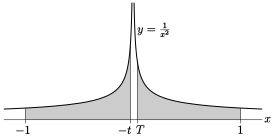
\includegraphics[width=\linewidth]{external/text/figs/boobyTrap.pdf}
\end{sbspanel}%
\end{sidebyside}%
\par
The full domain of integration is only recovered in the limit  \(t,T\rightarrow 0\).%
\item{}For this example, the correct computation is%
\begin{align*}
&\int_{-1}^1\frac{1}{x^2}\dee{x} =\lim_{t\rightarrow 0^+}\int_{-1}^{-t}\frac{1}{x^2}\dee{x} \ +\ \lim_{T\rightarrow 0^+}\int_{T}^{1}\frac{1}{x^2}\dee{x}\\
&\hskip0.25in=\lim_{t\rightarrow 0^+}\bigg[-\frac{1}{x}\bigg]_{-1}^{-t} +\lim_{T\rightarrow 0^+}\bigg[-\frac{1}{x}\bigg]_{T}^1\\
&\hskip0.25in=\lim_{t\rightarrow 0^+} \Big[\Big(-\frac{1}{-t}\Big)-\Big(-\frac{1}{-1}\Big)\Big] +\lim_{T\rightarrow 0^+} \Big[\Big(-\frac{1}{1}\Big)-\Big(-\frac{1}{T}\Big)\Big]\\
&\hskip0.25in=\lim_{t\rightarrow 0^+}\frac{1}{t} +\lim_{T\rightarrow 0^+}\frac{1}{T}-2\\
&\hskip0.25in=+\infty
\end{align*}
%
\item{}We can interpret this to mean that the signed area under the curve \(x^{-2}\) between  \(x=-1\) and \(x=1\) is infinite.%
\end{itemize}
%
\end{remark}
\end{example}
The above examples have illustrated how we can use the fundamental  theorem of calculus to convert knowledge of derivatives into  knowledge of integrals. We are now in a position to easily build a table of integrals. Here is a short table of the most important derivatives that we know.%
\begin{sidebyside}{1}{0}{0}{0}%
\begin{sbspanel}{1}%
\resizebox{\ifdim\width > \linewidth\linewidth\else\width\fi}{!}{%
{\centering%
{\tabularfont%
\begin{tabular}{AlAlAlAlAlAlAlAlAlAlA}\hrulethin
\(F(x)\)&\(1\)&\(x^n\)&\(\sin x\)&\(\cos x\)&\(\tan x\)&\(e^x\)&\(\log_e|x|\)&\(\arcsin x\)&\(\arctan x\)\tabularnewline\hrulethin
\(f(x)=F'(x)\)&\(0\)&\(nx^{n-1}\)&\(\cos x\)&\(-\sin x\)&\(\sec^2 x\)&\(e^x\)&\(\frac{1}{x}\)&\(\frac{1}{\sqrt{1-x^2}}\)&\(\frac{1}{1+x^2}\)\tabularnewline\hrulethin
\end{tabular}
}%
\par}
}%
\end{sbspanel}%
\end{sidebyside}%
\par
Of course we know other derivatives, such as those of \(\sec x\) and \(\cot x\), however the ones listed above are arguably the most important ones. From this table (with a very little massaging) we can write down a short table of indefinite integrals.%
\begin{theorem}{Theorem}{Important indefinite integrals.}{}{theorem-thm_imp_indef_int}%
\begin{center}%
{\tabularfont%
\begin{tabular}{AlAlA}\hrulethin
\(f(x)\)&\(F(x)=\int f(x)\dee{x}\)\tabularnewline\hrulethin
\(1\)&\(x+C\)\tabularnewline\hrulethin
\(x^n\)&\(\frac{1}{n+1}x^{n+1}+C\text{ provided that }n \ne-1\)\tabularnewline\hrulethin
\(\dfrac{1}{x}\)&\(\log_e|x|+C\)\tabularnewline\hrulethin
\(e^x\)&\(e^x+C\)\tabularnewline\hrulethin
\(\sin x\)&\(-\cos x+C\)\tabularnewline\hrulethin
\(\cos x\)&\(\sin x+C\)\tabularnewline\hrulethin
\(\sec^2 x\)&\(\tan x+C\)\tabularnewline\hrulethin
\(\dfrac{1}{\sqrt{1-x^2}}\)&\(\arcsin x+C\)\tabularnewline\hrulethin
\(\dfrac{1}{1+x^2}\)&\(\arctan x+C\)\tabularnewline\hrulethin
\end{tabular}
}%
\end{center}%
%
\end{theorem}
\begin{example}{Example}{Using Theorem {\xreffont\ref*{theorem-thm_imp_indef_int}} to compute some integrals.}{example-sec_fundamental-c-ap}%
Find the following integrals%
\begin{enumerate}[label=\roman*]
\item{}\(\displaystyle \int_2^7 e^x \dee{x}\)%
\item{}\(\displaystyle \int_{-2}^2 \frac{1}{1+x^2} \dee{x}\)%
\item{}\(\displaystyle \int_0^3 (2x^3+7x-2)\dee{x}\)%
\end{enumerate}
%
\par
\alert{Solution:} We can proceed with each of these as before \textemdash{} find the antiderivative and then  apply the fundamental theorem. The third integral is a little more complicated, but we  can split it up into monomials using Theorem~\hyperref[theorem-thm_Intarith]{{\xreffont\ref{theorem-thm_Intarith}}} and do each separately.%
\begin{enumerate}[label=\roman*]
\item{}An antiderivative of \(e^x\) is just \(e^x\), so%
\begin{align*}
\int_2^7 e^x \dee{x} &= e^x\bigg|_2^7\\
&= e^7-e^2 = e^2(e^5-1).
\end{align*}
%
\item{}An antiderivative of \(\frac{1}{1+x^2}\) is \(\arctan(x)\), so%
\begin{align*}
\int_{-2}^2 \frac{1}{1+x^2} \dee{x} &= \arctan(x) \bigg|_{-2}^2\\
&= \arctan(2) - \arctan(-2)\\
\intertext{We can simplify this a little further by noting that \(\arctan(x)\) is an  odd function, so \(\arctan(-2)= -\arctan(2)\) and thus our integral is}
&= 2\arctan(2)
\end{align*}
%
\item{}We can proceed by splitting the integral using Theorem~\hyperref[theorem-thm_Intarith]{{\xreffont\ref{theorem-thm_Intarith}}}(d)%
\begin{align*}
\int_0^3 (2x^3+7x-2)\dee{x} &= \int_0^3 2x^3\dee{x} + \int_0^3 7x\dee{x} - \int_0^3 2\dee{x}\\
&= 2\int_0^3 x^3\dee{x} + 7\int_0^3 x\dee{x} - 2\int_0^3 \dee{x}\\
\intertext{and because we know that \(x^4/4, x^2/2, x\) are antiderivatives of \(x^3, x, 1\)  respectively, this becomes}
&= \left[\frac{x^4}{2}\right]_0^3 + \left[\frac{7x^2}{2}\right]_0^3 - \left[2x\right]_0^3\\
&= \frac{81}{2} + \frac{7\cdot 9}{2} -6\\
&= \frac{81 + 63 - 12}{2} = \frac{132}{2} = 66.
\end{align*}
We can also just find the antiderivative of the whole polynomial by finding the  antiderivatives of each term of the polynomial and then recombining them. This is  equivalent to what we have done above, but perhaps a little neater:%
\begin{align*}
\int_0^3 (2x^3+7x-2)\dee{x} &= \left[ \frac{x^4}{2} + \frac{7x^2}{2} - 2x \right]_0^3\\
&= \frac{81}{2} + \frac{7\cdot 9}{2} -6 = 66.
\end{align*}
%
\end{enumerate}
%
\end{example}
\end{subsectionptx}
%
%
\typeout{************************************************}
\typeout{Exercises 1.3.2 Exercises}
\typeout{************************************************}
%
\begin{exercises-subsection}{Exercises}{Exercises}{}{Exercises}{}{}{exercises-sec_fundamental-d}
\par\medskip\noindent%
\textbf{.}\space\space%
Questions~\hyperlink{exercise-p1_1_FTC1}{11} through \hyperlink{exercise-p1_1_FTC2}{14} are meant to help reinforce key ideas in  the Fundamental Theorem of Calculus and its proof.%
So far, we have been able to guess many antiderivatives. Often, however, antiderivatives are very difficult to guess. In Questions~\hyperlink{exercise-p1_3_inttablea}{16} through \hyperlink{exercise-p1_3_inttableb}{19}, we will find some antiderivatives that might appear in a table of integrals. Coming up with the antiderivative might be quite difficult (strategies to do just that will form a large part of this semester), but \emph{verifying} that your antiderivative is correct is as simple as differentiating.%
\begin{exercisegroup}
\begin{divisionexerciseeg}{1}{2016Q2.}{}{exercise-sec_fundamental-d-a-c}%
Suppose that \(f(x)\) is a function and \(F(x) = e^{(x^2-3)} + 1\) is an antiderivative of \(f(x)\). Evaluate the definite integral \(\displaystyle\int_1^{\sqrt5} f(x)\,\dee{x}\).%
\end{divisionexerciseeg}%
\begin{divisionexerciseeg}{2}{M105 2015A.}{}{exercise-sec_fundamental-d-a-d}%
For the function \(f(x) = x^3 -\sin 2x\), find its antiderivative \(F(x)\) that satisfies \(F(0)=1\).%
\end{divisionexerciseeg}%
\footnotetext[9]{The symbol \(\iff\) is read ``if and only if''. This is used in mathematics to express the logical equivalence of two statements. To be more precise, the statement \(P \iff Q\) tells us that \(P\) is true whenever \(Q\) is true and \(Q\) is true whenever \(P\) is true.\label{fn-sec_fundamental-d-a-d-e-a-f}}%
\begin{divisionexerciseeg}{3}{2014D.}{}{exercise-sec_fundamental-d-a-e}%
Decide whether each of the following statements is true or false. Provide a brief justification.%
\par
%
\begin{enumerate}[label=\alph*]
\item{}If \(f(x)\) is continuous on \([1, \pi]\) and differentiable on \((1,\pi)\), then \(\displaystyle\int_1^\pi f'(x)\,\dee{x} = f(\pi)-f(1)\).%
\item{}\(\displaystyle\int_{-1}^1 \frac{1}{x^2}\,\dee{x} = 0\).%
\item{}If \(f\) is continuous on \([a, b]\) then \(\displaystyle\int_a^b xf(x)\,\dee{x} = x\int_a^b f(x)\,\dee{x} \).%
\end{enumerate}
%
\end{divisionexerciseeg}%
\begin{divisionexerciseeg}{4}{}{}{exercise-sec_fundamental-d-a-f}%
True or false: an antiderivative of \(\dfrac{1}{x^2}\) is \(\log (x^2)\) (where by \(\log x\) we mean logarithm base \(e\)).%
\end{divisionexerciseeg}%
\begin{divisionexerciseeg}{5}{}{}{exercise-sec_fundamental-d-a-g}%
True or false: an antiderivative of \(\cos(e^x)\) is \(\frac{\sin(e^x)}{e^x}\).%
\end{divisionexerciseeg}%
\begin{divisionexerciseeg}{6}{}{}{exercise-sec_fundamental-d-a-h}%
Suppose \(F(x) = \displaystyle\int_7^x \sin(t^2)\dee{t}\). What is the instantaneous rate of change of \(F(x)\) with respect to \(x\)?%
\end{divisionexerciseeg}%
\begin{divisionexerciseeg}{7}{}{}{exercise-sec_fundamental-d-a-i}%
Suppose \(F(x) = \displaystyle\int_{2}^x e^{1/t}\dee{t}\). What is the slope of the tangent line to \(y=F(x)\) when \(x=3\)?%
\end{divisionexerciseeg}%
\begin{divisionexerciseeg}{8}{}{}{exercise-sec_fundamental-d-a-j}%
Suppose \(F'(x)=f(x)\). Give two different antiderivatives of \(f(x)\).%
\end{divisionexerciseeg}%
\begin{divisionexerciseeg}{9}{}{}{exercise-sec_fundamental-d-a-k}%
In Question~\hyperlink{exercise-p1_1_awkwardcircle}{{\xreffont 1.1.8.45}}, Section~\hyperref[section-sec_intdef]{{\xreffont\ref{section-sec_intdef}}}, we found that%
\begin{equation*}
\int_0^a\sqrt{1-x^2}\dee{x}=\frac{\pi}{4} - \frac{1}{2}\arccos(a)+\frac{1}{2}a\sqrt{1-a^2}.
\end{equation*}
%
\par
%
\begin{enumerate}[label=\alph*]
\item{}Verify that \(\displaystyle\diff{}{a}\left\{\frac{\pi}{4} - \frac{1}{2}\arccos(a)+\frac{1}{2}a\sqrt{1-a^2}\right\} = \sqrt{1-a^2}\).%
\item{}Find a function \(F(x)\) that satisfies \(F'(x) = \sqrt{1-x^2}\) and \(F(0)=\pi\).%
\end{enumerate}
%
\end{divisionexerciseeg}%
\begin{divisionexerciseeg}{10}{}{}{exercise-sec_fundamental-d-a-l}%
Evaluate the following integrals using the Fundamental Theorem of Calculus Part 2, or explain why it does not apply.%
\begin{enumerate}[label=\alph*]
\item{}\(\displaystyle\int_{-\pi}^\pi \cos x \dee{x}\).%
\item{}\(\displaystyle\int_{-\pi}^\pi \sec^2 x \dee{x}\).%
\item{}\(\displaystyle\int_{-2}^0 \frac{1}{x+1}\dee{x}\).%
\end{enumerate}
%
\end{divisionexerciseeg}%
\begin{divisionexerciseeg}{11}{}{}{exercise-p1_1_FTC1}%
As in the proof of the Fundamental Theorem of Calculus, let \(F(x) = \int_{a}^x f(t)\dee{t}\). In the diagram below, shade the area corresponding to \(F(x+h)-F(x)\).%
\begin{sidebyside}{1}{0.2}{0.2}{0}%
\begin{sbspanel}{0.6}%
\resizebox{\linewidth}{!}{%
\begin{tikzpicture}
\YEtaaxis{1}{5}{1}{3}
\YExcoord{1}{a}
\YExcoord{2}{x}
\YExcoord{4}{x+h}
\draw[thick] plot[domain=.5:4.5] (\x,{3-(\x-3)*(\x-3)/2}) node[right]{$y=f(t)$};
\end{tikzpicture}
}%
\end{sbspanel}%
\end{sidebyside}%
\end{divisionexerciseeg}%
\begin{divisionexerciseeg}{12}{}{}{exercise-p1_1_intpic1}%
Let \(F(x) = \displaystyle\int_0^x f(t)\dee{t}\), where \(f(t)\) is shown in the graph below, and \(0 \leq x \leq 4\).%
\begin{enumerate}[label=\alph*]
\item{}Is \(F(0)\) positive, negative, or zero?%
\item{}Where is \(F(x)\) increasing and where is it decreasing?%
\end{enumerate}
%
\begin{sidebyside}{1}{0.25}{0.25}{0}%
\begin{sbspanel}{0.5}%
\resizebox{\linewidth}{!}{%
\begin{tikzpicture}
\YEtaaxis{1}{5}{3}{3}
\draw[thick] plot[domain=-1:4.3, samples=60] (\x,{(\x+.5)*(\x-1)*(\x-3)/(abs(\x)+1)});
\foreach \x in {1,...,4}{\YExcoord{\x}{\x}}
\draw (4,2) node[right] {$y=f(t)$};
\end{tikzpicture}
}%
\end{sbspanel}%
\end{sidebyside}%
\end{divisionexerciseeg}%
\begin{divisionexerciseeg}{13}{}{}{exercise-sec_fundamental-d-a-p}%
Let \(G(x) = \displaystyle\int_x^0 f(t)\dee{t}\), where \(f(t)\) is shown in the graph below, and \(0 \leq x \leq 4\).%
\begin{enumerate}[label=\alph*]
\item{}Is \(G(0)\) positive, negative, or zero?%
\item{}Where is \(G(x)\) increasing and where is it decreasing?%
\end{enumerate}
%
\begin{sidebyside}{1}{0.25}{0.25}{0}%
\begin{sbspanel}{0.5}%
\resizebox{\linewidth}{!}{%
\begin{tikzpicture}
\YEtaaxis{1}{5}{3}{3}
\draw[thick] plot[domain=-1:4.3, samples=60] (\x,{(\x+.5)*(\x-1)*(\x-3)/(abs(\x)+1)});
\foreach \x in {1,...,4}{\YExcoord{\x}{\x}}
\draw (4,2) node[right] {$y=f(t)$};
\end{tikzpicture}
}%
\end{sbspanel}%
\end{sidebyside}%
\end{divisionexerciseeg}%
\begin{divisionexerciseeg}{14}{}{}{exercise-p1_1_FTC2}%
Let \(F(x) = \displaystyle\int_a^x t\dee{t}\). Using the definition of the derivative, find \(F'(x)\).%
\end{divisionexerciseeg}%
\begin{divisionexerciseeg}{15}{}{}{exercise-sec_fundamental-d-a-r}%
Give a continuous function \(f(x)\) so that \(F(x) = \displaystyle\int_0^x f(t)\dee{t}\) is a constant.%
\end{divisionexerciseeg}%
\begin{divisionexerciseeg}{16}{}{}{exercise-p1_3_inttablea}%
Evaluate and simplify \(\diff{}{x}\{x\log(ax)-x\}\), where \(a\) is some constant and \(\log(x)\) is the logarithm base \(e\). What \emph{antiderivative} does this tell you?%
\end{divisionexerciseeg}%
\begin{divisionexerciseeg}{17}{}{}{exercise-sec_fundamental-d-a-u}%
Evaluate and simplify \(\diff{}{x}\{e^x\left(x^3-3x^2+6x-6\right)\}\). What \emph{antiderivative} does this tell you?%
\end{divisionexerciseeg}%
\begin{divisionexerciseeg}{18}{}{}{exercise-sec_fundamental-d-a-v}%
Evaluate and simplify \(\diff{}{x}\left\{\log\left|x+\sqrt{x^2+a^2}\right|\right\}\), where \(a\) is some constant. What \emph{antiderivative} does this tell you?%
\end{divisionexerciseeg}%
\begin{divisionexerciseeg}{19}{}{}{exercise-p1_3_inttableb}%
Evaluate and simplify \(\displaystyle\diff{}{x}\left\{\sqrt{x(a+x)}-a\log\left(\sqrt{x}+\sqrt{a+x}\right)\right\}\), where \(a\) is some constant. What \emph{antiderivative} does this tell you?%
\end{divisionexerciseeg}%
\end{exercisegroup}
\par\medskip\noindent
\par\medskip\noindent%
\textbf{.}\space\space%
\begin{exercisegroup}
\begin{divisionexerciseeg}{20}{2016Q2.}{}{exercise-sec_fundamental-d-b-c}%
Evaluate \(\displaystyle\int_0^2 \big(x^3+\sin x)\,\dee{x}\).%
\end{divisionexerciseeg}%
\begin{divisionexerciseeg}{21}{2012A.}{}{exercise-sec_fundamental-d-b-d}%
Evaluate \(\displaystyle\int_1^2 \frac{x^2+2}{x^2}\,\dee{x}\).%
\end{divisionexerciseeg}%
\begin{divisionexerciseeg}{22}{}{}{exercise-sec_fundamental-d-b-e}%
Evaluate \(\displaystyle\int \dfrac{1}{1+25x^2}\dee{x}\).%
\end{divisionexerciseeg}%
\begin{divisionexerciseeg}{23}{}{}{exercise-sec_fundamental-d-b-f}%
Evaluate \(\displaystyle\int \dfrac{1}{\sqrt{2-x^2}}\dee{x}\).%
\end{divisionexerciseeg}%
\begin{divisionexerciseeg}{24}{}{}{exercise-sec_fundamental-d-b-g}%
Evaluate \(\displaystyle\int \tan^2 x \dee{x}\).%
\end{divisionexerciseeg}%
\begin{divisionexerciseeg}{25}{}{}{exercise-sec_fundamental-d-b-h}%
Evaluate \(\displaystyle\int 3 \sin x \cos x \dee{x}\).%
\end{divisionexerciseeg}%
\begin{divisionexerciseeg}{26}{}{}{exercise-sec_fundamental-d-b-i}%
Evaluate \(\displaystyle\int \cos^2 x \dee{x}\).%
\end{divisionexerciseeg}%
\begin{divisionexerciseeg}{27}{M105 2012A.}{}{exercise-sec_fundamental-d-b-j}%
If%
\begin{equation*}
F(x)=\int_0^x \log(2+\sin t)\,\dee{t}\quad\text{and}\quad
G(y)=\int^0_y \log(2+\sin t)\,\dee{t}
\end{equation*}
find \(F'\big(\frac{\pi}{2}\big)\) and \(G'\big(\frac{\pi}{2}\big)\).%
\end{divisionexerciseeg}%
\begin{divisionexerciseeg}{28}{2014A.}{}{exercise-sec_fundamental-d-b-k}%
Let \(f(x)=\displaystyle\int_1^x 100(t^2-3t+2)e^{-t^2}\dee{t}\). Find the interval(s) on which \(f\) is increasing.%
\end{divisionexerciseeg}%
\begin{divisionexerciseeg}{29}{M105 2013A.}{}{exercise-sec_fundamental-d-b-l}%
If \(F(x)={\displaystyle\int_0^{\cos x} \frac{1}{t^3+6}\,\dee{t}}\), find \(F'(x)\).%
\end{divisionexerciseeg}%
\begin{divisionexerciseeg}{30}{1997D.}{}{exercise-sec_fundamental-d-b-m}%
Compute \(f'(x)\) where \(f(x)= \displaystyle\int_0^{1+x^4}e^{t^2}\dee{t}\).%
\end{divisionexerciseeg}%
\begin{divisionexerciseeg}{31}{M105 2015A.}{}{exercise-sec_fundamental-d-b-n}%
Evaluate \(\displaystyle\diff{}{x}\left\{\int_0^{\sin x}(t^6+8)\dee{t}\right\}\).%
\end{divisionexerciseeg}%
\begin{divisionexerciseeg}{32}{2000D.}{}{exercise-sec_fundamental-d-b-o}%
Let \(F(x)= \displaystyle\int_0^{x^3}e^{-t}\sin\left(\frac{\pi t}{2}\right)\,\dee{t}\). Calculate \(F'(1)\).%
\end{divisionexerciseeg}%
\begin{divisionexerciseeg}{33}{2016Q2.}{}{exercise-sec_fundamental-d-b-p}%
Find \(\displaystyle \diff{}{u} \left\{ \int_{\cos u}^0 \frac{\dee{t}}{1+t^3}
\right\}\).%
\end{divisionexerciseeg}%
\begin{divisionexerciseeg}{34}{M121 2000A.}{}{exercise-sec_fundamental-d-b-q}%
Find  \(f(x)\) if \(x^2=1+\displaystyle\int_1^x f(t)\dee{t}\).%
\end{divisionexerciseeg}%
\begin{divisionexerciseeg}{35}{2013A.}{}{exercise-sec_fundamental-d-b-r}%
If \(x \sin(\pi x) = \displaystyle\int_0^x f(t)\, \dee{t}\) where \(f\) is a continuous function, find \(f(4)\).%
\end{divisionexerciseeg}%
\begin{divisionexerciseeg}{36}{2016Q2.}{}{exercise-sec_fundamental-d-b-s}%
Consider the function \(\displaystyle F(x)=\int_0^{x^2} e^{-t}\,\dee{t} +\int_{-x}^0 e^{-t^2}\,\dee{t}\).%
\begin{enumerate}[label=\alph*]
\item{}Find \(F'(x)\).%
\item{}Find the value of \(x\) for which \(F(x)\) takes its minimum value.%
\end{enumerate}
%
\end{divisionexerciseeg}%
\begin{divisionexerciseeg}{37}{2016A.}{}{exercise-sec_fundamental-d-b-t}%
If \(F(x)\) is defined by \(\displaystyle F(x) = \int_{x^4-x^3}^x e^{\sin t}\,\dee{t}\), find \(F'(x)\).%
\end{divisionexerciseeg}%
\begin{divisionexerciseeg}{38}{M121 2012A.}{}{exercise-sec_fundamental-d-b-u}%
Evaluate \(\displaystyle \diff{}{x}\bigg\{\int_{x^5}^{-x^2} \cos\big(e^t\big)\,\dee{t} \bigg\}\).%
\end{divisionexerciseeg}%
\begin{divisionexerciseeg}{39}{2014D.}{}{exercise-sec_fundamental-d-b-v}%
Differentiate \(\displaystyle \int_x^{e^x} \sqrt{\sin t}\,\dee{t}\)  for \(0\lt x\lt \log \pi\).%
\end{divisionexerciseeg}%
\begin{divisionexerciseeg}{40}{M105 2014A.}{}{exercise-sec_fundamental-d-b-w}%
Evaluate \(\displaystyle \int_1^5 f(x)\,\dee{x}\), where \(\displaystyle f(x)= \begin{cases} 3 &\text{ if $x\le 3$} \\
x &\text{ if $x\ge 3$}
\end{cases}\).%
\end{divisionexerciseeg}%
\end{exercisegroup}
\par\medskip\noindent
\par\medskip\noindent%
\textbf{.}\space\space%
\begin{exercisegroup}
\begin{divisionexerciseeg}{41}{M105 2014A.}{}{exercise-sec_fundamental-d-c-c}%
If \(f'(1)=2\) and \(f'(2)=3\), find \(\displaystyle\int_1^2 f'(x) f''(x)\,\dee{x}\).%
\end{divisionexerciseeg}%
\begin{divisionexerciseeg}{42}{2016Q2.}{}{exercise-sec_fundamental-d-c-d}%
A car traveling at \(30\,\textrm{m}/\textrm{s}\) applies its brakes at time \(t=0\), its velocity (in \(\textrm{m}/\textrm{s}\)) decreasing according to the formula \(v(t) = 30 - 10t\). How far does the car go before it stops?%
\end{divisionexerciseeg}%
\begin{divisionexerciseeg}{43}{1998A.}{}{exercise-sec_fundamental-d-c-e}%
Compute \(f'(x)\) where \(f(x)= \displaystyle\int_0^{2x-x^2}\log\big(1+e^t\big)\,\dee{t}\). Does \(f(x)\) have an absolute maximum? Explain.%
\end{divisionexerciseeg}%
\begin{divisionexerciseeg}{44}{2001A.}{}{exercise-sec_fundamental-d-c-f}%
Find the minimum value of \(\displaystyle\int_0^{x^2-2x}\frac{\dee{t}}{1+t^4}\). Express your answer as an integral.%
\end{divisionexerciseeg}%
\begin{divisionexerciseeg}{45}{2001D.}{}{exercise-sec_fundamental-d-c-g}%
Define the function \(F(x)=\displaystyle\int_0^{x^2}\sin(\sqrt{t})\,\dee{t}\) on the interval \(0 \lt x \lt 4\). On this interval, where does \(F(x)\) have a maximum?%
\end{divisionexerciseeg}%
\begin{divisionexerciseeg}{46}{2002A.}{}{exercise-sec_fundamental-d-c-h}%
Evaluate \(\lim\limits_{n\rightarrow\infty}\dfrac{\pi}{n}\displaystyle\sum\limits_{j=1}^n
\sin\left(\frac{j\pi}{n}\right)\) by interpreting it as a limit of Riemann sums.%
\end{divisionexerciseeg}%
\begin{divisionexerciseeg}{47}{M121 2002A.}{}{exercise-sec_fundamental-d-c-i}%
Use Riemann sums to evaluate the limit \(\displaystyle\lim_{n\rightarrow\infty}\frac{1}{n}
\sum_{j=1}^n \frac{1}{1+\frac{j}{n}}\ .\)%
\end{divisionexerciseeg}%
\begin{divisionexerciseeg}{48}{}{}{exercise-sec_fundamental-d-c-j}%
Below is the graph of \(y=f(t)\), \(-5 \leq t \leq 5\). Define \(F(x) = \displaystyle\int_{0}^x f(t)\dee{t}\) for any \(x\) in \([-5,5]\). Sketch \(F(x)\).%
\begin{sidebyside}{1}{0.05}{0.05}{0}%
\begin{sbspanel}{0.9}%
\resizebox{\linewidth}{!}{%
\begin{tikzpicture}
\YEaaxis{6}{8}{2}{4}
\draw[thick, blue] plot[domain=-5:5, samples=100] (\x,{(\x*\x)/3+1)*cos(\x*1.57 r)/2}) node[above right]{$y=f(x)$};
\foreach \x in {-2.5,-1.5,-.5, .5, 1.5, 2.5}{
	\MULTIPLY{\x}{2}{\l}
	\YExcoord{\l}{\l}}
\end{tikzpicture}
}%
\end{sbspanel}%
\end{sidebyside}%
\end{divisionexerciseeg}%
\begin{divisionexerciseeg}{49}{2015A.}{}{exercise-sec_fundamental-d-c-k}%
Define \(f(x)=x^3\displaystyle\int_{0}^{x^3+1} e^{t^3} \dee{t}\).%
\begin{enumerate}[label=\alph*]
\item{}Find a formula for the derivative \(f'(x)\). (Your formula may include an integral sign.)%
\item{}Find the equation of the tangent line to the graph of \(y=f(x)\) at \(x=-1\).%
\end{enumerate}
%
\end{divisionexerciseeg}%
\begin{divisionexerciseeg}{50}{}{}{exercise-sec_fundamental-d-c-l}%
Two students calculate \(\int f(x)\dee{x}\) for some function \(f(x)\).%
\begin{itemize}[label=\textbullet]
\item{}Student A calculates \(\int f(x)\dee{x} = \tan^2 x + x + C\)%
\item{}Student B calculates \(\int f(x)\dee{x} = \sec^2 x + x + C\)%
\item{}It is a fact that \(\diff{}{x}\{\tan^2 x\} = f(x)-1\)%
\end{itemize}
Who ended up with the correct answer?%
\end{divisionexerciseeg}%
\begin{divisionexerciseeg}{51}{}{}{exercise-sec_fundamental-d-c-m}%
Let \(F(x)=\displaystyle\int_0^x x^3 \sin(t)\dee{t}\).%
\begin{enumerate}[label=\alph*]
\item{}Evaluate \(F(3)\).%
\item{}What is \(F'(x)\)?%
\end{enumerate}
%
\end{divisionexerciseeg}%
\begin{divisionexerciseeg}{52}{}{}{exercise-sec_fundamental-d-c-n}%
Let \(f(x)\) be an even function, defined everywhere, and let \(F(x)\) be an antiderivative of \(f(x)\). Is \(F(x)\) even, odd, or not necessarily either one? (You may use your answer from Section~\hyperref[section-sec_def_int]{{\xreffont\ref{section-sec_def_int}}}, Question~\hyperlink{exercise-p1_2_derivevenodd}{{\xreffont 1.2.3.20}}. )%
\end{divisionexerciseeg}%
\end{exercisegroup}
\par\medskip\noindent
\end{exercises-subsection}
\end{sectionptx}
%
%
\typeout{************************************************}
\typeout{Section 1.4 Substitution}
\typeout{************************************************}
%
\begin{sectionptx}{Section}{Substitution}{}{Substitution}{}{}{section-sec_subs}
\begin{introduction}{}%
\end{introduction}%
%
%
\typeout{************************************************}
\typeout{Subsection 1.4.1 Substitution}
\typeout{************************************************}
%
\begin{subsectionptx}{Subsection}{Substitution}{}{Substitution}{}{}{subsection-sec_subs-c}
In the previous section we explored the fundamental theorem of calculus and the link it  provides between definite integrals and antiderivatives. Indeed, integrals with simple  integrands are usually evaluated via this link. In this section we start to explore  methods for integrating more complicated integrals. We have already seen \textemdash{}  via Theorem~\hyperref[theorem-thm_Intarith]{{\xreffont\ref{theorem-thm_Intarith}}} \textemdash{} that integrals interact very nicely with  addition, subtraction and multiplication by constants:%
\begin{align*}
\int_a^b \left( Af(x) + B g(x) \right) \dee{x} &= A\int_a^b f(x)\dee{x} + B\int_a^b g(x)\dee{x}
\end{align*}
for \(A,B\) constants. By combining this with the list of indefinite integrals in  Theorem~\hyperref[theorem-thm_imp_indef_int]{{\xreffont\ref{theorem-thm_imp_indef_int}}}, we can compute integrals of linear combinations of  simple functions. For example%
\begin{align*}
\int_1^4\left(e^x - 2\sin x + 3x^2 \right)\dee{x} &= \int_1^4e^x\dee{x} -2\int_1^4 \sin x \dee{x} +3 \int_1^4x^2 \dee{x}\\
&= \left(e^x  + (-2)\cdot(-\cos x) + 3\frac{x^3}{3} \right)\bigg|_1^4  &\text{and so on}
\end{align*}
Of course there are a great many functions that can be approached in this way, however  there are some very simple examples that cannot.%
\begin{align*}
\int \sin(\pi x) \dee{x} && \int x e^x \dee{x} && \int \frac{x}{x^2-5x+6}\dee{x}
\end{align*}
In each case the integrands are not linear combinations of simpler functions; in order to  compute them we need to understand how integrals (and antiderivatives) interact with  compositions, products and quotients. We reached a very similar point in our differential  calculus course where we understood the linearity of the derivative,%
\begin{align*}
\diff{}{x}\left(Af(x)+ Bg(x)\right) &= A\diff{f}{x} + B\diff{g}{x},
\end{align*}
but had not yet seen the chain, product and quotient rules \footnote{If your memory of  these rules is a little hazy then you really should go back and revise them before  proceeding. You will definitely need a good grasp of the chain rule for what follows in this section.\label{fn-sec_subs-c-b-l}}. While we will develop tools to find the second and third integrals in  later sections, we should really start with how to integrate compositions of functions.%
\par
It is important to state up front, that in general one cannot write down the integral of  the composition of two functions \textemdash{} even if those functions are simple. This is not  because the integral does not exist. Rather it is because the integral cannot be written  down as a finite combination of the standard functions we know. A very good example of  this, which we encountered in Example~\hyperref[example-eg_INTftocA]{{\xreffont\ref{example-eg_INTftocA}}}, is the composition of \(e^x\) and  \(-x^2\). Even though we know%
\begin{align*}
\int e^x \dee{x} &= e^x+C & \text{and}&&  \int -x^2 \dee{x} &= -\frac13 x^3 +C
\end{align*}
there is no simple function that is equal to the indefinite integral%
\begin{gather*}
\int e^{-x^2}\dee{x}.
\end{gather*}
even though the indefinite integral exists. In this way integration is very different  from differentiation.%
\par
With that caveat out of the way, we can introduce the substitution rule. The substitution  rule is obtained by antidifferentiating the chain rule. In some sense it is the chain  rule  in reverse. For completeness, let us restate the chain rule:%
\begin{theorem}{Theorem}{The chain rule.}{}{theorem-sec_subs-c-e}%
Let \(F(u)\) and \(u(x)\) be differentiable functions and form their composition \(F(u(x))\).  Then%
\begin{align*}
\diff{}{x} F\big( u( x) \big) &= F'\big(u(x)\big) \cdot u'(x)
\end{align*}
Equivalently, if \(y(x)=F(u(x))\), then%
\begin{align*}
\diff{y}{x} &= \diff{F}{u} \cdot \diff{u}{x}.
\end{align*}
%
\end{theorem}
Consider a function \(f(u)\), which has antiderivative \(F(u)\). Then we know  that%
\begin{align*}
\int f(u) \dee{u} &= \int F'(u) \dee{u} = F(u) +C
\end{align*}
Now take the above equation and substitute into it \(u=u(x)\) \textemdash{} i.e. replace the  variable \(u\) with any (differentiable) function of \(x\) to get%
\begin{align*}
\int f(u) \dee{u}\bigg|_{u=u(x)} &= F(u(x)) +C
\end{align*}
But now the right-hand side is a function of \(x\), so we can differentiate it with respect  to \(x\) to get%
\begin{align*}
\diff{}{x} F(u(x)) &= F'(u(x)) \cdot u'(x)
\end{align*}
This tells us that \(F(u(x))\) is an antiderivative of the function \(F'(u(x))\cdot u'(x)  = f(u(x))u'(x)\). Thus we know%
\begin{align*}
\int f\big(u(x)\big) \cdot u'(x)\,\dee{x}  &= F\big(u(x)\big) +C = \int f(u)\,\dee{u}\bigg|_{u=u(x)}
\end{align*}
This is the substitution rule for indefinite integrals.%
\begin{theorem}{Theorem}{The substitution rule \textemdash{} indefinite integral version.}{}{theorem-thm_subs_indef}%
For any differentiable function \(u(x)\):%
\begin{align*}
\int f(u(x)) u'(x) \dee{x} &= \int f(u)\dee{u}\bigg|_{u=u(x)}
\end{align*}
%
\end{theorem}
In order to apply the substitution rule successfully we will have to write the integrand  in the form \(f(u(x))\cdot u'(x)\). To do this we need to make a good choice of the  function \(u(x)\); after that it is not hard to then find \(f(u)\) and \(u'(x)\).   Unfortunately there is no one strategy for choosing \(u(x)\). This can make applying the  substitution rule more art than science \footnote{Thankfully this does become easier with  experience and we recommend that the reader read some examples and then practice a LOT.\label{fn-sec_subs-c-h-f}}. Here we suggest two possible strategies for picking \(u(x)\):%
\begin{enumerate}[label=\arabic*]
\item{}Factor the integrand and choose one of the factors to be \(u'(x)\). For this to work,  you must be able to easily find the antiderivative of the chosen factor. The  antiderivative will be \(u(x)\).%
\item{}Look for a factor in the integrand that is a function with an argument that is more  complicated than just ``\(x\)''. That factor will play the role of \(f\big(u(x)\big)\) Choose  \(u(x)\) to be the complicated argument.%
\end{enumerate}
Here are two examples which illustrate each of those strategies in turn.%
\begin{example}{Example}{\(\int 9\sin^8(x) \cos(x) \dee{x}\).}{example-sec_subs-c-i}%
Consider the integral%
\begin{gather*}
\int 9\sin^8(x) \cos(x) \dee{x}
\end{gather*}
We want to massage this into the form of the integrand in the substitution rule \textemdash{} namely  \(f(u(x))\cdot u'(x)\). Our integrand can be written as the product of the two factors%
\begin{gather*}
\underbrace{9 \sin^8(x)}_\text{first factor} \cdot  \underbrace{\cos(x)}_\text{second factor}
\end{gather*}
and we start by determining (or guessing) which factor plays the role of  \(u'(x)\). We can choose \(u'(x)=9\sin^8(x)\) or \(u'(x)=\cos(x)\).%
\begin{itemize}[label=\textbullet]
\item{}If we choose \(u'(x)=9\sin^8(x)\), then antidifferentiating this to find \(u(x)\) is  really not very easy. So it is perhaps better to investigate the other choice before  proceeding further with this one.%
\item{}If we choose \(u'(x)=\cos(x)\), then we know (Theorem~\hyperref[theorem-thm_imp_indef_int]{{\xreffont\ref{theorem-thm_imp_indef_int}}}) that  \(u(x)=\sin(x)\). This also works nicely because it makes the other factor  simplify quite a bit \(9\sin^8(x) = 9u^8\). This looks like the right way to go.%
\end{itemize}
So we go with the second choice. Set \(u'(x)=\cos(x), u(x)=\sin(x)\), then%
\begin{align*}
\int 9\sin^8(x) \cos(x) \dee{x}
&= \int 9u(x)^8 \cdot u'(x) \dee{x}\\
&= \int 9u^8 \dee{u} \bigg|_{u=\sin(x)} & \text{by the substitution rule}\\
\intertext{We are now left with the problem of  antidifferentiating a monomial; this we can  do with Theorem \hyperref[theorem-thm_imp_indef_int]{{\xreffont\ref{theorem-thm_imp_indef_int}}}.}
&= \left( u^9 +C \right)\bigg|_{u=\sin(x)}\\
&= \sin^9(x) +C
\end{align*}
Note that \(9\sin^8(x) \cos(x)\) is a function of \(x\). So our answer, which is the  indefinite integral of  \(9\sin^8(x) \cos(x)\), must also be a function of \(x\).  This is why we have substituted \(u=\sin(x)\) in the last step of our solution \textemdash{} it  makes our solution a function of \(x\).%
\end{example}
\begin{example}{Example}{\(\int 3x^2 \cos(x^3) \dee{x}\).}{example-sec_subs-c-j}%
Evaluate the integral%
\begin{gather*}
\int 3x^2 \cos(x^3) \dee{x}
\end{gather*}
%
\par
\alert{Solution:} Again we are going to use the substitution rule and helpfully our integrand is a  product of two factors%
\begin{gather*}
\underbrace{3x^2}_\text{first factor} \cdot  \underbrace{\cos(x^3)}_\text{second factor}
\end{gather*}
The second factor, \(\cos\big(x^3\big)\) is a function, namely \(\cos\), with a complicated  argument, namely \(x^3\). So we try \(u(x)= x^3\). Then \(u'(x) = 3x^2\), which is the other  factor in the integrand. So the integral becomes%
\begin{align*}
\int 3x^2 \cos(x^3) \dee{x} &= \int u'(x) \cos\big(u(x)\big) \dee{x} &\text{just swap order of factors}\\
&= \int \cos\big(u(x)\big) u'(x) \dee{x} & \text{by the substitution rule}\\
&= \int \cos(u) \dee{u}\bigg|_{u=x^3}\\
&= \left( \sin(u) + C\right)\bigg|_{u=x^3}  & \text{using Theorem }\hyperref[theorem-thm_imp_indef_int]{\text{{\xreffont\ref{theorem-thm_imp_indef_int}}}})\\
&= \sin(x^3)+C
\end{align*}
%
\end{example}
One more \textemdash{} we'll use this to show how to use the substitution rule with definite  integrals.%
\begin{example}{Example}{\(\int_0^1 e^x\sin(e^x)\dee{x}\).}{example-eg_substitution1}%
Compute%
\begin{gather*}
\int_0^1 e^x\sin\big(e^x\big)\dee{x}.
\end{gather*}
%
\par
\alert{Solution:} Again we use the substitution rule.%
\begin{itemize}[label=\textbullet]
\item{}The integrand is again the product of two factors and we can choose \(u'(x)=e^x\) or  \(u'(x)=\sin(e^x)\).%
\item{}If we choose \(u'(x)=e^x\) then \(u(x)=e^x\) and the other factor becomes \(\sin(u)\) \textemdash{}  this looks promising. Notice that if we applied the other strategy of looking for a  complicated argument then we would arrive at the same choice.%
\item{}So we try \(u'(x)=e^x\) and \(u(x)=e^x\). This gives (if we ignore the limits of  integration for a moment)%
\begin{align*}
\int e^x \sin\big(e^x\big)\dee{x}
&= \int \sin\big(u(x)\big) u'(x) \dee{x} &\text{apply the substitution rule}\\
&= \int \sin(u)\dee{u} \bigg|_{u=e^x}\\
&= \left(-\cos(u)+C \right)\bigg|_{u=e^x}\\
&= -\cos\big(e^x\big) +C
\end{align*}
%
\item{}But what happened to the limits of integration? We can incorporate them now. We  have just shown that the indefinite integral is \(-\cos(e^x)\), so by the fundamental  theorem of calculus%
\begin{align*}
\int_0^1 e^x\sin\big(e^x\big)\dee{x}
&= \big[-\cos\big(e^x\big)\big]_0^1\\
&= -\cos(e^1)-(-\cos(e^0))\\
&= -\cos(e)+\cos(1)
\end{align*}
%
\end{itemize}
%
\end{example}
Theorem~\hyperref[theorem-thm_subs_indef]{{\xreffont\ref{theorem-thm_subs_indef}}}, the substitution rule for indefinite integrals, tells us  that if \(F(u)\) is any antiderivative for \(f(u)\), then \(F\big(u(x)\big)\) is an  antiderivative for \(f\big(u(x)\big) u'(x)\). So the fundamental theorem of calculus gives  us%
\begin{align*}
\int_a^b f\big(u(x)\big) u'(x)\,\dee{x} &= F\big(u(x)\big)\bigg|_{x=a}^{x=b}\\
&= F\big(u(b)\big) - F\big(u(a)\big)\\
&= \int_{u(a)}^{u(b)} f(u)\,\dee{u} & \text{since $F(u)$ is an antiderivative for $f(u)$}
\end{align*}
and we have just found%
\begin{theorem}{Theorem}{The substitution rule \textemdash{} definite integral version.}{}{theorem-thm_subs_def}%
For any differentiable function \(u(x)\):%
\begin{align*}
\int_a^b f(u(x)) u'(x) \dee{x} &= \int_{u(a)}^{u(b)} f(u)\dee{u}
\end{align*}
%
\end{theorem}
Notice that to get from the integral on the left hand side to the integral on the right  hand side you%
\begin{itemize}[label=\textbullet]
\item{}substitute \footnote{A good way to remember this last step is that we  replace \(\diff{u}{x} \dee{x}\) by just \(\dee{u}\) \textemdash{} which looks  like we cancelled out the \(\dee{x}\) terms: \(\frac{\dee{u}}{\cancel{\dee{x}}}\cancel{\dee{x}} = \dee{u}\). While using ``cancel the  \(\dee{x}\)'' is a good mnemonic (memory aid), you should not think of the derivative  \(\diff{u}{x}\) as a fraction \textemdash{} you are not dividing \(\dee{u}\) by \(\dee{x}\).\label{fn-sec_subs-c-o-a-a-a}} \(u(x)\rightarrow u\) and  \(u'(x)\dee{x}\rightarrow \dee{u}\),%
\item{}set the lower limit for the \(u\) integral to the value of \(u\) (namely \(u(a)\)) that corresponds to the lower limit of the \(x\)  integral (namely \(x=a\)), and%
\item{}set the upper limit for the \(u\) integral to the value of \(u\) (namely \(u(b)\)) that corresponds to the upper limit of the \(x\)  integral (namely \(x=b\)).%
\end{itemize}
Also note that we now have two ways to evaluate definite integrals of the form \(\int_a^b f\big(u(x)\big)u'(x)\,\dee{x}\).%
\begin{itemize}[label=\textbullet]
\item{}We can find the indefinite integral \(\int f\big(u(x)\big) u'(x)\,\dee{x}\), using  Theorem~\hyperref[theorem-thm_subs_indef]{{\xreffont\ref{theorem-thm_subs_indef}}}, and then evaluate the result between \(x=a\) and \(x=b\). This  is what was done in Example~\hyperref[example-eg_substitution1]{{\xreffont\ref{example-eg_substitution1}}}.%
\item{}Or we can apply Theorem~\hyperref[theorem-thm_subs_indef]{{\xreffont\ref{theorem-thm_subs_indef}}}. This entails finding the  indefinite integral \(\int f(u)\,\dee{u}\) and evaluating the result between \(u=u(a)\) and  \(u=u(b)\). This is what we will do in the following example.%
\end{itemize}
%
\begin{example}{Example}{\(\int_0^1 x^2\sin(x^3+1)\dee{x}\).}{example-eg_substitution2}%
Compute%
\begin{gather*}
\int_0^1 x^2\sin\big(x^3+1\big)\dee{x}
\end{gather*}
%
\par
\alert{Solution:}%
\begin{itemize}[label=\textbullet]
\item{}In this example the integrand is already neatly factored into two pieces. While we  could deploy either of our two strategies, it is perhaps easier in this case to  choose \(u(x)\) by looking for a complicated argument.%
\item{}The second factor of the integrand is \(\sin\big(x^3+1\big)\), which is the function  \(\sin\) evaluated at \(x^3+1\). So set \(u(x)=x^3+1\), giving \(u'(x)=3x^2\) and \(f(u)=\sin(u)\)%
\item{}The first factor of the integrand is \(x^2\) which is not quite \(u'(x)\), however we  can easily massage the integrand into the required form by multiplying and dividing by \(3\):%
\begin{align*}
x^2\sin\big(x^3+1\big) &= \frac{1}{3} \cdot 3x^2\cdot \sin\big(x^3+1\big).
\end{align*}
%
\item{}We want this in the form of the substitution rule, so we do a little massaging:%
\begin{align*}
\int_0^1 x^2\sin\big(x^3+1\big)\dee{x}
&= \int_0^1 \frac{1}{3}\cdot 3x^2 \cdot \sin\big(x^3+1\big)\dee{x}\\
&= \frac{1}{3}\int_0^1 \sin\big(x^3+1\big)\cdot 3x^2 \dee{x}\\
&\hskip1.5in\text{by Theorem }\hyperref[theorem-thm_Intarith]{\text{{\xreffont\ref{theorem-thm_Intarith}}}}\text{(c)}
\end{align*}
%
\item{}Now we are ready for the substitution rule:%
\begin{align*}
\frac{1}{3}\int_0^1 \sin\big(x^3+1\big)\cdot 3x^2 \dee{x}
&=\frac{1}{3}\int_0^1 \underbrace{\sin\big(x^3+1\big)}_{=f(u(x))}\cdot
\underbrace{3x^2}_{=u'(x)} \dee{x}\\
\intertext{Now set \(u(x)=x^3+1\) and \(f(u)=\sin(u)\)}
&= \frac{1}{3}\int_0^1 f(u(x)) u'(x) \dee{x}\\
&= \frac{1}{3} \int_{u(0)}^{u(1)} f(u) \dee{u} & \text{by the substitution rule}\\
&= \frac{1}{3} \int_{1}^{2} \sin(u) \dee{u}  & \text{since $u(0)=1$ and
$u(1)=2$}\\
&= \frac{1}{3} \big[-\cos(u)\big]_1^2\\
&= \frac{1}{3}\big( -\cos(2) -(-\cos(1)) \big)\\
&= \frac{\cos(1)-\cos(2)}{3}.
\end{align*}
%
\end{itemize}
%
\end{example}
There is another, and perhaps easier, way to view the manipulations in the previous  example. Once you have chosen \(u(x)\) you%
\begin{itemize}[label=\textbullet]
\item{}make the substitution \(u(x) \rightarrow u\),%
\item{}replace \(\dee{x} \rightarrow \dfrac{1}{u'(x)} \dee{u}\).%
\end{itemize}
In so doing, we take the integral%
\begin{align*}
\int_a^b f(u(x)) \cdot u'(x) \dee{x}
&= \int_{u(a)}^{u(b)} f(u) \cdot u'(x) \cdot \frac{1}{u'(x)} \dee{u}\\
&= \int_{u(a)}^{u(b)} f(u) \dee{u} & \text{exactly the substitution rule}
\end{align*}
but we do not have to manipulate the integrand so as to make \(u'(x)\) explicit.  Let us  redo the previous example by this approach.%
\begin{example}{Example}{Example {\xreffont\ref*{example-eg_substitution2}} revisited.}{example-eg_substitution3}%
Compute the integral%
\begin{gather*}
\int_0^1 x^2\sin\big(x^3+1\big)\dee{x}
\end{gather*}
%
\par
\alert{Solution:}%
\begin{itemize}[label=\textbullet]
\item{}We have already observed that one factor of the integrand is  \(\sin\big(x^3+1\big)\), which is \(\sin\) evaluated at \(x^3+1\). Thus we try setting  \(u(x)=x^3+1\).%
\item{}This makes \(u'(x)=3x^2\), and we replace \(u(x)=x^3+1\rightarrow u\) and  \(\dee{x}\rightarrow\frac{1}{u'(x)}\dee{u} = \frac{1}{3x^2}\dee{u}\):%
\begin{align*}
\int_0^1 x^2\sin\big(x^3+1\big)\dee{x}
&= \int_{u(0)}^{u(1)} x^2\underbrace{\sin\big(x^3+1\big)}_{=\sin(u)}
\frac{1}{3x^2}\dee{u}\\
&= \int_{1}^{2} \sin(u) \frac{x^2}{3x^2}\dee{u}\\
&= \int_{1}^{2} \frac{1}{3}\sin(u) \dee{u}\\
&= \frac{1}{3}\int_{1}^{2} \sin(u) \dee{u}
\end{align*}
which is precisely the integral we found in Example~\hyperref[example-eg_substitution2]{{\xreffont\ref{example-eg_substitution2}}}.%
\end{itemize}
%
\end{example}
\begin{example}{Example}{Some more substitutions.}{example-sec_subs-c-s}%
Compute the indefinite integrals%
\begin{align*}
\int \sqrt{2x+1}\dee{x} && \text{and} && \int e^{3x-2}\dee{x}
\end{align*}
%
\par
\alert{Solution:}%
\begin{itemize}[label=\textbullet]
\item{}Starting with the first integral, we see that it is not too hard to spot  the complicated argument. If we set \(u(x)=2x+1\) then the integrand is just \(\sqrt{u}\).%
\item{}Hence we substitute \(2x+1 \rightarrow u\) and \(\dee{x} \rightarrow  \frac{1}{u'(x)}\dee{u}=\frac{1}{2}\dee{u}\):%
\begin{align*}
\int \sqrt{2x+1}\dee{x}
&= \int \sqrt{u} \frac{1}{2} \dee{u}\\
&= \int u^{1/2} \frac{1}{2} \dee{u}\\
&= \left( \frac{2}{3}u^{3/2}\cdot\frac{1}{2}  +C\right)\bigg|_{u=2x+1}\\
&= \frac{1}{3} (2x+1)^{3/2} + C
\end{align*}
%
\item{}We can evaluate the second integral in much the same way. Set \(u(x)=3x-2\) and  replace \(\dee{x}\) by \(\frac{1}{u'(x)}\dee{u} = \frac{1}{3}\dee{u}\):%
\begin{align*}
\int e^{3x-2}\dee{x}
&= \int e^u \frac{1}{3}\dee{u}\\
&= \left( \frac{1}{3} e^u + C\right)\bigg|_{u=3x-2}\\
&= \frac{1}{3} e^{3x-2} +C
\end{align*}
%
\end{itemize}
%
\end{example}
This last example illustrates that substitution can be used to easily deal with arguments  of the form \(ax+b\), i.e. that are linear functions of \(x\), and suggests the following  theorem.%
\begin{theorem}{Theorem}{}{}{theorem-thm_subs_linear}%
Let \(F(u)\) be an antiderivative of \(f(u)\) and let \(a,b\) be constants. Then%
\begin{align*}
\int f(ax+b)\dee{x} &= \frac{1}{a} F(ax+b) +C
\end{align*}
%
\end{theorem}
\begin{proof}{Proof}{}{proof-sec_subs-c-v}
We can show this using the substitution rule. Let \(u(x)=ax+b\) so \(u'(x)=a\), then%
\begin{align*}
\int f(ax+b) \dee{x}
&= \int f(u) \cdot \frac{1}{u'(x)}\dee{u}\\
&= \int \frac{1}{a} f(u) \dee{u}\\
&= \frac{1}{a} \int f(u) \dee{u} & \text{since $a$ is a constant}\\
&= \frac{1}{a} F(u)\bigg|_{u=ax+b} +C & \text{since $F(u)$ is an antiderivative of
$f(u)$}\\
&= \frac{1}{a} F(ax+b) +C.\qedhere
\end{align*}
%
\end{proof}
Now we can do the following example using the substitution rule or the above theorem:%
\begin{example}{Example}{\(\int_0^{\frac{\pi}{2}}\cos(3x)\dee{x}\).}{example-eg_substitution4}%
Compute \(\int_0^{\frac{\pi}{2}}\cos(3x)\dee{x}\).%
\par
%
\begin{itemize}[label=\textbullet]
\item{}In this example we should set \(u=3x\), and substitute \(\dee{x} \rightarrow  \frac{1}{u'(x)}\dee{u} = \frac{1}{3}\dee{u}.\) When we do this we also have to convert  the limits of the integral: \(u(0)=0\) and \(u(\pi/2)=3\pi/2\). This gives%
\begin{align*}
\int_0^{\frac{\pi}{2}}\cos(3x)\dee{x}
&= \int_0^{\frac{3\pi}{2}} \cos(u) \frac{1}{3}\dee{u}\\
&= \left[\frac{1}{3} \sin(u) \right]_0^{\frac{3\pi}{2}}\\
&= \frac{\sin(3\pi/2)-\sin(0)}{3}\\
&= \frac{-1-0}{3} = - \frac{1}{3}.
\end{align*}
%
\item{}We can also do this example more directly using the above theorem. Since \(\sin(x)\)  is an antiderivative of \(\cos(x)\), Theorem~\hyperref[theorem-thm_subs_linear]{{\xreffont\ref{theorem-thm_subs_linear}}} tells us that  \(\frac{\sin(3x)}{3}\) is an antiderivative of \(\cos(3x)\). Hence%
\begin{align*}
\int_0^{\frac{\pi}{2}}\cos(3x)\dee{x}
&= \left[ \frac{\sin(3x)}{3} \right]_0^{\frac{\pi}{2}}\\
&= \frac{\sin(3\pi/2)-\sin(0)}{3}\\
&= -\frac{1}{3}.
\end{align*}
%
\end{itemize}
%
\end{example}
The rest of this section is just more examples of the substitution rule. We recommend  that you after reading these that you practice many examples by yourself under exam  conditions.%
\begin{example}{Example}{\(\int_0^1 x^2\sin(1-x^3)\dee{x}\).}{example-eg_substitution3neg}%
This integral looks a lot like that of Example \hyperref[example-eg_substitution2]{{\xreffont\ref{example-eg_substitution2}}}. It makes  sense to try \(u(x)=1-x^3\) since it is the argument of \(\sin(1-x^3)\). We%
\begin{itemize}[label=\textbullet]
\item{}substitute \(u=1-x^3\) and%
\item{}replace \(\dee{x}\) with \(\frac{1}{u'(x)}\dee{u} = \frac{1}{-3x^2}\dee{u}\),%
\item{}when \(x=0\), we have \(u=1-0^3=1\) and%
\item{}when \(x=1\), we have \(u=1-1^3=0\).%
\end{itemize}
So%
\begin{align*}
\int_0^1 x^2 \sin\big(1-x^3\big)\cdot \dee{x} &=\int_1^0 x^2 \sin(u) \cdot \frac{1}{-3x^2}\dee{u}\\
&= \int_1^0 -\frac{1}{3}\sin(u)\dee{u}.\\
\intertext{Note that the lower limit of the \(u\)-integral, namely \(1\), is larger than the upper limit, which is \(0\). There is absolutely nothing wrong with that. We can simply evaluate the \(u\)-integral in the normal way. Since \(-\cos(u)\) is an antiderivative  of \(\sin(u)\):}
&=  \left[\frac{\cos(u)}{3} \right]_1^0\\
&= \frac{\cos(0)-\cos(1)}{3}\\
&= \frac{1-\cos(1)}{3}.
\end{align*}
%
\end{example}
\begin{example}{Example}{\(\int_0^1\frac{1}{(2x+1)^3}\dee{x}\).}{example-eg_substitution5}%
Compute \(\int_0^1\frac{1}{(2x+1)^3}\dee{x}\).%
\par
We could do this one using Theorem~\hyperref[theorem-thm_subs_linear]{{\xreffont\ref{theorem-thm_subs_linear}}}, but its not too hard to do  without. We can think of the integrand as the function ``one over a cube'' with the argument \(2x+1\). So it makes sense to substitute \(u=2x+1\). That is%
\begin{itemize}[label=\textbullet]
\item{}set \(u=2x+1\) and%
\item{}replace \(\dee{x} \rightarrow \frac{1}{u'(x)}\dee{u} =  \frac{1}{2}\dee{u}\).%
\item{}When \(x=0\), we have \(u=2\times 0+1=1\) and%
\item{}when \(x=1\), we have \(u=2\times 1+1=3\).%
\end{itemize}
So%
\begin{align*}
\int_0^1\frac{1}{(2x+1)^3}\dee{x} &=\int_1^{3} \frac{1}{u^3} \cdot \frac{1}{2}\dee{u}\\
&=\frac{1}{2}\int_1^{3}u^{-3}\dee{u}\\
&=\frac{1}{2}\left[\frac{u^{-2}}{-2}\right]_1^{3}\\
&=\frac{1}{2}\left( \frac{1}{-2}\cdot \frac{1}{9} - \frac{1}{-2}\cdot\frac{1}{1}  \right)\\
&=\frac{1}{2}\left( \frac{1}{2} - \frac{1}{18}\right) = \frac{1}{2}\cdot \frac{8}{18}\\
&=\frac{2}{9}
\end{align*}
%
\end{example}
\begin{example}{Example}{\(\int_0^1\frac{x}{1+x^2}\dee{x}\).}{example-eg_substitution6}%
Evaluate \(\int_0^1\frac{x}{1+x^2}\dee{x}\).%
\par
\alert{Solution:}%
\begin{itemize}[label=\textbullet]
\item{}The integrand can be rewritten as \(x \cdot \frac{1}{1+x^2}\). This second factor  suggests that we should try setting \(u=1+x^2\) \textemdash{} and so we interpret the  second factor as the function ``one over'' evaluated at argument \(1+x^2\).%
\item{}With this choice we%
\begin{itemize}[label=$\circ$]
\item{}set \(u=1+x^2\),%
\item{}substitute \(\dee{x} \rightarrow \frac{1}{2x}\dee{u}\), and%
\item{}translate the limits of integration: when \(x=0\), we have \(u=1+0^2=1\) and when  \(x=1\), we have \(u=1+1^2=2\).%
\end{itemize}
%
\item{}The integral then becomes%
\begin{align*}
\int_0^1\frac{x}{1+x^2}\dee{x}
&= \int_1^2 \frac{x}{u} \frac{1}{2x}\dee{u}\\
&= \int_1^2 \frac{1}{2u} \dee{u}\\
&= \frac{1}{2} \big[ \log|u| \big]_1^2\\
&= \frac{\log 2 - \log 1}{2} = \frac{\log 2}{2}.
\end{align*}
%
\end{itemize}
Remember that we are using the notation ``\(\log\)'' for the natural logarithm, i.e. the logarithm with base \(e\). You might also see it written as ``\(\ln  x\)'', or with the base made explicit as ``\(\log_e x\)''.%
\end{example}
\begin{example}{Example}{\(\int x^3\cos\big(x^4+2\big)\dee{x}\).}{example-eg_substitution7}%
Compute the integral \(\int x^3\cos\big(x^4+2\big)\dee{x}\).%
\par
\alert{Solution:}%
\begin{itemize}[label=\textbullet]
\item{}The integrand is the product of \(\cos\) evaluated at the argument \(x^4+2\) times  \(x^3\), which aside from a factor of \(4\), is the derivative of the argument \(x^4+2\).%
\item{}Hence we set \(u=x^4+2\) and then substitute \(\dee{x} \rightarrow  \frac{1}{u'(x)}\dee{u} = \frac{1}{4x^3}\dee{u}\).%
\item{}Before proceeding further, we should note that  this is an indefinite integral so  we  don't have to worry about the limits of integration. However we do need to make sure our  answer is a function of \(x\) \textemdash{} we cannot leave it as a function of \(u\).%
\item{}With this choice of \(u\), the integral then becomes%
\begin{align*}
\int x^3\cos\big(x^4+2\big)\dee{x} &= \int x^3 \cos(u) \frac{1}{4x^3}\dee{u} \bigg|_{u=x^4+2}\\
&=  \int\frac{1}{4} \cos(u) \dee{u} \bigg|_{u=x^4+2}\\
&= \left(\frac{1}{4}\sin(u)+C\right)\bigg|_{u=x^4+2}\\
&= \frac{1}{4}\sin(x^4+2) +C.
\end{align*}
%
\end{itemize}
%
\end{example}
The next two examples are more involved and require more careful thinking.%
\begin{example}{Example}{\(\int \sqrt{1+x^2}\,x^3\dee{x}\).}{example-eg_substitution8}%
Compute \(\int \sqrt{1+x^2}\,x^3\dee{x}\).%
\par
%
\begin{itemize}[label=\textbullet]
\item{}An obvious choice of \(u\) is the argument inside the square root. So substitute  \(u=1+x^2\) and \(\dee{x} \rightarrow \frac{1}{2x}\dee{u}\).%
\item{}When we do this we obtain%
\begin{align*}
\int \sqrt{1+x^2}\cdot x^3\dee{x}
&= \int \sqrt{u}\cdot x^3 \cdot \frac{1}{2x}\dee{u}\\
&= \int \frac{1}{2} \sqrt{u}\cdot x^2 \dee{u}
\end{align*}
Unlike all our previous examples, we have not cancelled out all of the \(x\)'s from the  integrand. However before we do the integral with respect to \(u\), the integrand must be  expressed solely in terms of \(u\) \textemdash{} no \(x\)'s are allowed. (Look that integrand on the  right hand side of Theorem~\hyperref[theorem-thm_subs_indef]{{\xreffont\ref{theorem-thm_subs_indef}}}.)%
\item{}But all is not lost. We can rewrite the factor \(x^2\) in terms of the variable \(u\).  We know that \(u=1+x^2\), so this means \(x^2 = u-1\). Substituting this into our integral  gives%
\begin{align*}
\int \sqrt{1+x^2}\cdot x^3\dee{x}
&= \int \frac{1}{2} \sqrt{u}\cdot x^2 \dee{u}\\
&= \int \frac{1}{2} \sqrt{u}\cdot (u-1) \dee{u}\\
&= \frac{1}{2} \int \left(u^{3/2}-u^{1/2}\right) \dee{u}\\
&= \frac{1}{2} \left( \frac{2}{5} u^{5/2} - \frac{2}{3}u^{3/2} \right)\bigg|_{u=x^2+1}
+C\\
&= \left(\frac{1}{5} u^{5/2} - \frac{1}{3}u^{3/2}\right) \bigg|_{u=x^2+1}  +C\\
&= \frac{1}{5}(x^2+1)^{5/2} - \frac{1}{3} (x^2+1)^{3/2} +C.
\end{align*}
Oof!%
\item{}Don't forget that you can always check the answer by differentiating:%
\begin{align*}
& \diff{}{x} \left( \frac{1}{5}(x^2+1)^{5/2} - \frac{1}{3} (x^2+1)^{3/2} +C\right)\\
&= \diff{}{x} \left( \frac{1}{5}(x^2+1)^{5/2} \right) -
\diff{}{x} \left( \frac{1}{3}(x^2+1)^{3/2} \right)\\
&= \frac{1}{5} \cdot 2x \cdot \frac{5}{2} \cdot (x^2+1)^{3/2} -
\frac{1}{3} \cdot 2x \cdot \frac{3}{2} \cdot (x^2+1)^{1/2}\\
&= x (x^2+1)^{3/2} - x(x^2+1)^{1/2}\\
&= x  \big[ (x^2+1)-1 \big] \cdot\sqrt{x^2+1}\\
&= x^3 \sqrt{x^2+1}.
\end{align*}
which is the original integrand \(\checkmark\).%
\end{itemize}
%
\end{example}
\begin{example}{Example}{\(\int \tan x\dee{x}\).}{example-eg_substitution9}%
Evaluate the indefinite integral \(\int \tan(x) \dee{x}\).%
\par
\alert{Solution:}%
\begin{itemize}[label=\textbullet]
\item{}At first glance there is nothing to manipulate here and so very little to go on.  However we can rewrite \(\tan x\) as \(\frac{\sin x}{\cos x}\), making the integral \(\int  \frac{\sin x}{\cos x}\dee{x}\). This gives us more to work with.%
\item{}Now think of the integrand as being the product \(\frac{1}{\cos x}\cdot \sin  x\). This suggests that we set \(u=\cos x\) and that we interpret the first factor as the  function ``one over'' evaluated at \(u=\cos x\).%
\item{}Substitute \(u = \cos x\) and \(\dee{x} \rightarrow \frac{1}{-\sin x}\dee{u}\) to give:%
\begin{align*}
\int \frac{\sin x}{\cos x}\dee{x}
&=\int \frac{\sin x}{u} \frac{1}{-\sin x} \dee{u} \bigg|_{u=\cos x}\\
&= \int -\frac{1}{u}\dee{u}  \bigg|_{u=\cos x}\\
&= -\log|\cos x| +C & \text{and if we want to go further}\\
&= \log\left|\frac{1}{\cos x} \right|+C\\
&= \log|\sec x| +C.
\end{align*}
%
\end{itemize}
%
\end{example}
In all of the above substitution examples we expressed the new integration variable, \(u\), as a function, \(u(x)\), of the old integration variable \(x\). It is also possible to express the old integration variable, \(x\), as a function, \(x(u)\), of the new integration variable \(u\). We shall see examples of this in Section~\hyperref[section-sec_trigsub]{{\xreffont\ref{section-sec_trigsub}}}.%
\end{subsectionptx}
%
%
\typeout{************************************************}
\typeout{Exercises 1.4.2 Exercises}
\typeout{************************************************}
%
\begin{exercises-subsection}{Exercises}{Exercises}{}{Exercises}{}{}{exercises-sec_subs-d}
\begin{introduction}{}%
Recall that we are using \(\log x\) to denote the logarithm of \(x\) with base \(e\). In other courses it is often denoted \(\ln x\).%
\end{introduction}%
\par\medskip\noindent%
\textbf{.}\space\space%
\begin{exercisegroup}
\begin{divisionexerciseeg}{1}{}{}{exercise-p1_4_intbounds}%
%
\begin{enumerate}[label=\alph*]
\item{}True or False: \(\displaystyle\int \sin(e^x)\cdot e^x\dee{x} = \left.\displaystyle\int \sin(u)\dee u\right|_{u=e^x} = -\cos(e^x)+C\)%
\item{}True or False: \(\displaystyle\int_0^1 \sin(e^x)\cdot e^x\dee{x} = \displaystyle\int_0^1 \sin(u)\dee u = 1-\cos(1)\)%
\end{enumerate}
%
\end{divisionexerciseeg}%
\begin{divisionexerciseeg}{2}{}{}{exercise-sec_subs-d-b-d}%
Is the following reasoning sound? If not, fix it.%
\begin{quote}%
\emph{Problem:} Evaluate \(\displaystyle\int (2x+1)^2 \dee{x}\).%
\par
\emph{Work:} We use the substitution \(u=2x+1\). Then:%
\begin{align*}
\int (2x+1)^2 \dee{x}&=\int u^2\dee{u}\\
&=\frac{1}{3}u^3+C\\
&=\frac{1}{3}\left(2x+1\right)^3+C
\end{align*}
%
\end{quote}
\end{divisionexerciseeg}%
\begin{divisionexerciseeg}{3}{}{}{exercise-sec_subs-d-b-e}%
Is the following reasoning sound? If not, fix it.%
\begin{quote}%
\emph{Problem:} Evaluate \(\displaystyle\int_{1}^{\pi} \dfrac{\cos(\log t)}{t}\dee{t}\).%
\par
\emph{Work:} We use the substitution \(u=\log t\), so \(\dee{u}=\frac{1}{t}\dee{t}\). Then:%
\begin{align*}
\int_{1}^{\pi} \dfrac{\cos(\log t)}{t}\dee{t}&=\int_1^{\pi}\cos(u) \dee{u}\\
&=\sin(\pi)-\sin(1)=-\sin(1)\, .
\end{align*}
%
\end{quote}
\end{divisionexerciseeg}%
\begin{divisionexerciseeg}{4}{}{}{exercise-sec_subs-d-b-f}%
Is the following reasoning sound? If not, fix it.%
\begin{quote}%
\emph{Problem:} Evaluate \(\displaystyle\int_{0}^{\pi/4} x\tan (x^2) \dee{x}\).%
\par
\emph{Work:} We begin with the substitution \(u=x^2\),  \(\dee{u} = 2x\dee{x}\):%
\begin{align*}
\int_{0}^{\pi/4} x\tan (x^2) \dee{x}&= \int_{0}^{\pi/4} \frac{1}{2}\tan(x^2)\cdot 2x\dee{x}\\
&=\int_{0}^{\pi^2/16} \frac{1}{2}\tan u\dee{u}\\
&=\frac{1}{2}\int_{0}^{\pi^2/16} \dfrac{\sin u}{\cos u}\dee{u}\\
\intertext{Now we use the substitution \(v=\cos u\), \(\dee{v}=-\sin u \dee{u}\):}
&=\frac{1}{2}\int_{\cos 0}^{\cos(\pi^2/16)} -\dfrac{1}{v}\dee{v}\\
&=-\frac{1}{2}\int_{1}^{\cos(\pi^2/16)} \dfrac{1}{v}\dee{v}\\
&=-\frac{1}{2}\left[\log|v|\right]_{1}^{\cos(\pi^2/16)}\\
& =-\frac{1}{2}\left(\log\left(\cos(\pi^2/16)\right)-\log(1)\right)\\
&=-\frac{1}{2}\log\left(\cos(\pi^2/16)\right)
\end{align*}
%
\end{quote}
\end{divisionexerciseeg}%
\begin{divisionexerciseeg}{5}{2016A.}{}{exercise-sec_subs-d-b-g}%
What is the integral that results when the substitution \(u= \sin x\)   is applied to the integral \(\displaystyle \int_0^{\pi/2} f(\sin x)\,\dee{x}\)?%
\end{divisionexerciseeg}%
\begin{divisionexerciseeg}{6}{}{}{exercise-sec_subs-d-b-h}%
Let \(f\) and \(g\) be functions that are continuous and differentiable everywhere. Simplify%
\begin{equation*}
\int f'(g(x))g'(x)\dee{x} - f(g(x)).
\end{equation*}
%
\end{divisionexerciseeg}%
\end{exercisegroup}
\par\medskip\noindent
\par\medskip\noindent%
\textbf{.}\space\space%
\begin{exercisegroup}
\begin{divisionexerciseeg}{7}{2016Q2.}{}{exercise-sec_subs-d-c-c}%
Use substitution to evaluate \(\displaystyle\int_{0}^{1} x e^{x^2} \cos (e^{x^2}) \,\dee{x}\).%
\end{divisionexerciseeg}%
\begin{divisionexerciseeg}{8}{2001D.}{}{exercise-sec_subs-d-c-d}%
Let \(f(t)\) be any function for which \(\displaystyle\int_1^8 f(t)\,\dee{t}=1\). Calculate the integral \(\displaystyle\int_1^2 x^2 f(x^3)\,\dee{x}\).%
\end{divisionexerciseeg}%
\begin{divisionexerciseeg}{9}{M121 2014A.}{}{exercise-sec_subs-d-c-e}%
Evaluate \(\displaystyle \int  \frac{x^2}{{(x^3+1)}^{101}}\dee{x}\).%
\end{divisionexerciseeg}%
\begin{divisionexerciseeg}{10}{2016Q2.}{}{exercise-sec_subs-d-c-f}%
Evaluate \(\displaystyle \int_{e}^{e^4} \frac{\dee{x}}{x\log x}\).%
\end{divisionexerciseeg}%
\begin{divisionexerciseeg}{11}{2012A.}{}{exercise-sec_subs-d-c-g}%
Evaluate \(\displaystyle \int_{0}^{\pi/2} \frac{\cos x} {1+\sin x}\,\dee{x}\).%
\end{divisionexerciseeg}%
\begin{divisionexerciseeg}{12}{2016Q2.}{}{exercise-sec_subs-d-c-h}%
Evaluate \(\displaystyle \int_{0}^{\pi/2} \cos x \cdot (1+\sin^2 x)\,\dee{x}\).%
\end{divisionexerciseeg}%
\begin{divisionexerciseeg}{13}{2013A.}{}{exercise-sec_subs-d-c-i}%
Evaluate \(\displaystyle\int_1^3(2x-1)e^{x^2-x}\dee{x}\).%
\end{divisionexerciseeg}%
\begin{divisionexerciseeg}{14}{2016Q2.}{}{exercise-sec_subs-d-c-j}%
Evaluate \({\displaystyle \int \frac{(x^2-4)x}{\sqrt{4-x^2}}\,\dee{x}}\).%
\end{divisionexerciseeg}%
\begin{divisionexerciseeg}{15}{}{}{exercise-sec_subs-d-c-k}%
Evaluate \(\displaystyle\int \dfrac{e^{\sqrt{\log x}}}{2x\sqrt{\log x}}\dee{x}\,.\)%
\end{divisionexerciseeg}%
\end{exercisegroup}
\par\medskip\noindent
\par\medskip\noindent%
\textbf{.}\space\space%
Questions~\hyperlink{exercise-p1_4_roughsuba}{18} through \hyperlink{exercise-p1_4_roughsubb}{22} can be solved by substitution, but it may not be obvious which substitution will work. In general, when evaluating integrals, it is not always immediately clear which methods are appropriate. If this happens to you, don't despair, and definitely don't give up! Just guess a method and try it. Even if it fails, you'll probably learn something that you can use to make a better guess. \footnote{This is also pretty decent life advice.\label{fn-sec_subs-d-d-e-a-d}}%
\begin{exercisegroup}
\begin{divisionexerciseeg}{16}{2016A.}{}{exercise-sec_subs-d-d-c}%
Calculate \(\displaystyle\int_{-2}^2 xe^{x^2}\,\dee{x}\).%
\end{divisionexerciseeg}%
\begin{divisionexerciseeg}{17}{2000D.}{}{exercise-sec_subs-d-d-d}%
Calculate \(\displaystyle\lim\limits_{n\rightarrow\infty}\sum\limits_{j=1}^n
\dfrac{j}{n^2}\sin\left(1+\dfrac{j^2}{n^2}\right)\).%
\end{divisionexerciseeg}%
\begin{divisionexerciseeg}{18}{}{}{exercise-p1_4_roughsuba}%
Evaluate \(\displaystyle\int_{0}^1 \dfrac{u^3}{u^2+1}\dee{u}\).%
\end{divisionexerciseeg}%
\begin{divisionexerciseeg}{19}{}{}{exercise-sec_subs-d-d-g}%
Evaluate \(\displaystyle\int \tan^3 \theta\  \dee{\theta}\).%
\end{divisionexerciseeg}%
\begin{divisionexerciseeg}{20}{}{}{exercise-sec_subs-d-d-h}%
Evaluate \(\displaystyle\int \dfrac{1}{e^x+e^{-x}}\dee{x}\)%
\end{divisionexerciseeg}%
\begin{divisionexerciseeg}{21}{}{}{exercise-sec_subs-d-d-i}%
Evaluate \(\displaystyle\int_0^1 (1-2x)\sqrt{1-x^2}\dee{x}\)%
\end{divisionexerciseeg}%
\begin{divisionexerciseeg}{22}{}{}{exercise-p1_4_roughsubb}%
Evaluate \(\displaystyle\int\tan x \cdot \log\left(\cos x\right) \dee{x}\)%
\end{divisionexerciseeg}%
\begin{divisionexerciseeg}{23}{2001A.}{}{exercise-sec_subs-d-d-k}%
Evaluate \(\displaystyle\lim\limits_{n\rightarrow\infty}
\sum\limits_{j=1}^n \dfrac{j}{n^2}\cos\left(\dfrac{j^2}{n^2}\right)\).%
\end{divisionexerciseeg}%
\begin{divisionexerciseeg}{24}{2001D.}{}{exercise-sec_subs-d-d-l}%
Calculate \(\displaystyle\lim\limits_{n\rightarrow\infty}\sum\limits_{j=1}^n
\frac{j}{n^2}\sqrt{1+\frac{j^2}{n^2}}\).%
\end{divisionexerciseeg}%
\begin{divisionexerciseeg}{25}{}{}{exercise-sec_subs-d-d-m}%
Using Riemann sums, prove that%
\begin{equation*}
\int_a^b 2f(2x)\dee{x} = \int_{2a}^{2b} f(x)\dee{x}
\end{equation*}
%
\end{divisionexerciseeg}%
\end{exercisegroup}
\par\medskip\noindent
\end{exercises-subsection}
\end{sectionptx}
%
%
\typeout{************************************************}
\typeout{Section 1.5 Area between curves}
\typeout{************************************************}
%
\begin{sectionptx}{Section}{Area between curves}{}{Area between curves}{}{}{section-sec_area}
\begin{introduction}{}%
\end{introduction}%
%
%
\typeout{************************************************}
\typeout{Subsection 1.5.1 Area between curves}
\typeout{************************************************}
%
\begin{subsectionptx}{Subsection}{Area between curves}{}{Area between curves}{}{}{subsection-sec_area-c}
Before we continue our exploration of different methods for integrating functions, we  have now have sufficient tools to examine some simple applications of definite integrals.  One of the motivations for our definition of ``integral'' was the problem of finding the area between some curve and the \(x\)-axis for \(x\) running between two specified values. More precisely%
\begin{gather*}
\int_a^b f(x) \dee{x}
\end{gather*}
is equal to the signed area between the the curve \(y=f(x)\), the \(x\)-axis, and the  vertical lines \(x=a\) and \(x=b\).%
\par
We found the area of this region by approximating it by the union of tall thin  rectangles,  and then found the exact area by taking the limit as the width of the approximating  rectangles went to zero. We can use the same strategy to find areas of more  complicated regions in the \(xy\)-plane.%
\par
As a preview of the material to come, let \(f(x) \gt g(x) \gt 0\) and \(a \lt b\) and suppose that we are  interested in the area of the region%
\begin{gather*}
S_1=\big\{\ (x,y)\ \big|\ a\le x\le b\,,\, g(x)\le y\le f(x)\ \big\}
\end{gather*}
that is sketched in the left hand figure below.%
\begin{sidebyside}{1}{0.05}{0.05}{0}%
\begin{sbspanel}{0.9}%
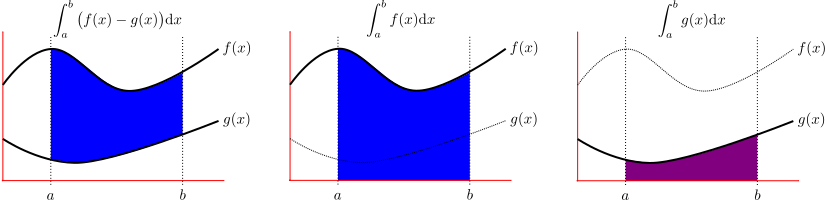
\includegraphics[width=\linewidth]{external/text/figs/area_between2.pdf}
\end{sbspanel}%
\end{sidebyside}%
\par
We already know that \(\int_a^b f(x)\,\dee{x}\) is the area of the region%
\begin{gather*}
S_2=\big\{\ (x,y)\ \big|\ a\le x\le b\,,\, 0\le y\le f(x)\ \big\}
\end{gather*}
sketched in the middle figure above and that \(\int_a^b g(x)\,\dee{x}\) is the area of the  region%
\begin{gather*}
S_3=\big\{\ (x,y)\ \big|\ a\le x\le b\,,\, 0\le y\le g(x)\ \big\}
\end{gather*}
sketched in the right hand figure above. Now the region \(S_1\) of the left hand figure  can be constructed by taking the region \(S_2\) of center figure and removing from it the  region \(S_3\) of the right hand figure. So the area of \(S_1\) is exactly%
\begin{align*}
\int_a^b f(x)\,\dee{x} -  \int_a^b g(x)\,\dee{x}
&=  \int_a^b \big(f(x)-g(x)\big)\,\dee{x}
\end{align*}
This computation depended on the assumption that \(f(x) \gt g(x)\) and, in particular, that the curves \(y=g(x)\) and \(y=f(x)\) did not cross. If they do cross, as in this figure%
\begin{sidebyside}{1}{0.3}{0.3}{0}%
\begin{sbspanel}{0.4}%
\includegraphics[width=\linewidth]{external/text/figs/area_between1a.pdf}
\end{sbspanel}%
\end{sidebyside}%
\par
then we have to be a lot more careful. The idea is to separate the domain of  integration depending on where \(f(x) - g(x)\) changes sign \textemdash{} i.e. where the curves  intersect. We will illustrate this in Example~\hyperref[example-eg_AREAc]{{\xreffont\ref{example-eg_AREAc}}} below.%
\par
Let us start with an example that makes the link to Riemann sums and definite integrals quite explicit.%
\begin{example}{Example}{The area between \(y=4-x^2\) and \(y=x\).}{example-eg_areabetween_riemann}%
Find the area bounded by the curves \(y=4-x^2\), \(y=x\), \(x=-1\) and \(x=1\).%
\par
\alert{Solution:}%
\begin{itemize}[label=\textbullet]
\item{}Before we do any calculus, it is a very good idea to make a sketch of the area in  question. The curves \(y=x\), \(x=-1\) and \(x=1\) are all straight lines, while the curve  \(y=4-x^2\) is a parabola whose apex is at \((0,4)\) and then curves down  (because of the  minus sign in \(-x^2\)) with \(x\)-intercepts at \((\pm2,0)\). Putting these together gives%
\begin{sidebyside}{1}{0.17}{0.17}{0}%
\begin{sbspanel}{0.66}%
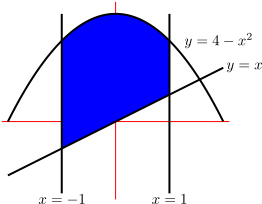
\includegraphics[width=\linewidth]{external/text/figs/area_between3.pdf}
\end{sbspanel}%
\end{sidebyside}%
\par
Notice that the curves \(y=4-x^2\) and \(y=x\) intersect when \(4-x^2=x\), namely when \(x= \frac{1}{2}\left(-1\pm\sqrt{17}\right) \approx 1.56,-2.56\). Hence the curve \(y=4-x^2\)  lies above the line \(y=x\) for all \(-1\le x\le 1\).%
\item{}We are to find the area of the shaded region. Each point \((x,y)\) in this  shaded region has \(-1\le x\le 1\) and \(x \le y \le 4-x^2\). When we were defining the integral (way back in Definition~\hyperref[definition-def_INTintegral]{{\xreffont\ref{definition-def_INTintegral}}}) we used \(a\) and \(b\)  to denote the smallest and largest allowed values of \(x\); let's do that here too.  Let's also use \(B(x)\) to denote the bottom curve (i.e. to denote the smallest allowed  value of \(y\) for a given \(x\)) and use \(T(x)\) to denote the top curve (i.e. to denote the  largest allowed value of \(y\) for a given \(x\)). So in this example%
\begin{align*}
a=-1&& b=1&& B(x)=x&& T(x)=4-x^2
\end{align*}
and the shaded region is%
\begin{gather*}
\big\{\ (x,y)\ \big|\ a\le x\le b,\ B(x)\le y\le T(x)\ \big\}
\end{gather*}
%
\item{}We use the same strategy as we used when defining the integral in  Section~\hyperref[subsection-sec_defInt]{{\xreffont\ref{subsection-sec_defInt}}}:%
\begin{itemize}[label=$\circ$]
\item{}Pick a natural number \(n\) (that we will later send to infinity), then%
\item{}subdivide the region into \(n\) narrow slices, each of width \(\De x=\frac{b-a}{n}\).%
\item{}For each \(i=1,2,\cdots,n\), slice number \(i\) runs from \(x=x_{i-1}\) to \(x=x_i\), and we  approximate its area by the area of a rectangle. We pick a number \(x_i^*\) between  \(x_{i-1}\) and \(x_i\) and approximate the slice by a rectangle whose top is at \(y=T(x_i^*)\)  and whose bottom is at \(y=B(x_i^*)\).%
\item{}Thus the area of slice \(i\) is approximately \(\big[T(x_i^*)-B(x_i^*)\big]\De x\) (as  shown in the figure below).%
\end{itemize}
%
\begin{sidebyside}{1}{0.17}{0.17}{0}%
\begin{sbspanel}{0.66}%
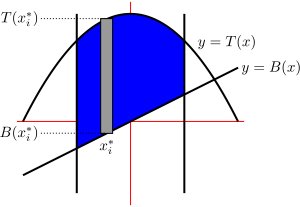
\includegraphics[width=\linewidth]{external/text/figs/area_between4.pdf}
\end{sbspanel}%
\end{sidebyside}%
\item{}So the Riemann sum approximation of the area is%
\begin{align*}
\text{Area} &\approx \sum_{i=1}^n  \big[T(x_i^*)-B(x_i^*)\big]\De x
\end{align*}
%
\item{}By taking the limit as \(n \to \infty\) (i.e. taking the limit as the width of the  rectangles goes to zero), we convert the Riemann sum into a definite integral (see  Definition~\hyperref[definition-def_INTintegral]{{\xreffont\ref{definition-def_INTintegral}}}) and at the same time our approximation of the area  becomes the exact area:%
\begin{align*}
\lim_{n\rightarrow\infty}\sum_{i=1}^n  \big[T(x_i^*)-B(x_i^*)\big]\De x
&=\int_a^b \big[T(x)-B(x)\big]\dee{x} \\
&\hskip1in \text{Riemann sum $\to$ integral}\\
&=\int_{-1}^1\big[(4-x^2)-x\big]\dee{x}\\
&=\int_{-1}^1\big[4-x-x^2\big]\dee{x}\\
&=\bigg[4x - \frac{x^2}{2} - \frac{x^3}{3} \bigg]_{-1}^1\\
&= \left(4 - \frac{1}{2}-\frac{1}{3} \right) - \left(-4-\frac{1}{2}+\frac{1}{3} \right)\\
&= \frac{24-3-2}{6} - \frac{-24-3+2}{6}\\
&= \frac{19}{6} + \frac{25}{6}\\
&= \frac{44}{6} = \frac{22}{3}.
\end{align*}
%
\end{itemize}
%
\end{example}
Oof! Thankfully we generally do not need to go through the Riemann sum steps to get to  the answer. Usually, provided we are careful to check where curves intersect and which  curve lies above which, we can just jump straight to the integral%
\begin{equation*}
\text{Area} = \int_a^b \big[T(x)-B(x)\big]\dee{x}.
\end{equation*}
So let us redo the above example.%
\begin{example}{Example}{Example {\xreffont\ref*{example-eg_areabetween_riemann}} revisited.}{example-eg_areabetween_riemann_again}%
Find the area bounded by the curves \(y=4-x^2\), \(y=x\), \(x=-1\) and \(x=1\).%
\par
\alert{Solution:}%
\begin{itemize}[label=\textbullet]
\item{}We first sketch the region%
\begin{sidebyside}{1}{0.17}{0.17}{0}%
\begin{sbspanel}{0.66}%
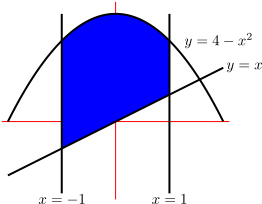
\includegraphics[width=\linewidth]{external/text/figs/area_between3.pdf}
\end{sbspanel}%
\end{sidebyside}%
\par
and verify \footnotemark{} that \(y=T(x)=4-x^2\) lies above the curve \(y=B(x)=x\) on the region \(-1\leq x\leq 1\).%
\item{}The area between the curves is then%
\begin{align*}
\text{Area} &= \int_a^b \big[T(x)-B(x)\big]\dee{x}\\
&=\int_{-1}^1\big[4-x-x^2\big]\dee{x}\\
&=\bigg[4x - \frac{x^2}{2} - \frac{x^3}{3} \bigg]_{-1}^1\\
&= \frac{19}{6} + \frac{25}{6} = \frac{44}{6} = \frac{22}{3}.
\end{align*}
%
\end{itemize}
%
\end{example}
\footnotetext[1]{We should do this by checking where the curves intersect; that is by  solving \(T(x)=B(x)\) and seeing if any of the solutions lie in the range \(-1\leq x \leq  1\).\label{fn-eg_areabetween_riemann_again-c-b-a-c-a}}%
\begin{example}{Example}{The area between \(y=x^2\) and  \(y=6x-2x^2\).}{example-eg_AREAa}%
Find the area of the finite region bounded by \(y=x^2\) and  \(y=6x-2x^2\).%
\par
\alert{Solution:} This is a little different from the previous question, since we are not given  bounding lines \(x=a\) and \(x=b\) \textemdash{} instead we have to determine the minimum and maximum  allowed values of \(x\) by determining where the curves intersect. Hence our very first  task is to get a good idea of what the region looks like by sketching it.%
\begin{itemize}[label=\textbullet]
\item{}Start by sketching the region:%
\begin{itemize}[label=$\circ$]
\item{}The curve \(y=x^2\) is a parabola. The point on this parabola with the  smallest \(y\)-coordinate is \((0,0)\). As \(|x|\) increases, \(y\) increases so the parabola opens upward.%
\item{}The curve \(y=6x-2x^2 =-2(x^2-3x) =-2(x-\frac{3}{2})^2+\frac{9}{2}\) is also a   parabola. The point on this parabola with the largest value of \(y\) has  \(x=\frac{3}{2}\)  (so that the negative term in \(-2(x-\frac{3}{2})^2+\frac{9}{2}\) is zero). So the point  with the largest value of \(y\) is is \((\frac{3}{2},\frac{9}{2})\). As \(x\) moves  away  from \(\frac{3}{2}\), either to the right or to the left, \(y\) decreases. So the  parabola  opens downward. The parabola crosses the \(x\)-axis when \(0=6x-2x^2=2x(3-x)\). That is,  when  \(x=0\) and \(x=3\).%
\item{}The two parabolas intersect when \(x^2= 6x-2x^2\), or%
\begin{align*}
3x^2-6x&=0\\
3x(x-2)&=0
\end{align*}
So there are two points of intersection, one being \(x=0\), \(y=0^2=0\) and the other being \(x=2\), \(y=2^2=4\).%
\item{}The finite region between the curves lies between these two points of  intersection.%
\end{itemize}
This leads us to the sketch%
\begin{sidebyside}{1}{0.25}{0.25}{0}%
\begin{sbspanel}{0.5}%
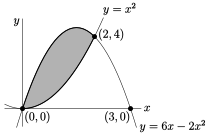
\includegraphics[width=\linewidth]{external/text/figs/areaSMPL.pdf}
\end{sbspanel}%
\end{sidebyside}%
\item{}So on this region we have \(0\leq x\leq 2\), the top curve is \(T(x)=6x-x^2\) and the  bottom curve is \(B(x)=x^2\). Hence the area is given by%
\begin{align*}
\text{Area} &=\int_a^b \big[T(x)-B(x)\big]\dee{x}\\
&=\int_0^2\big[(6x-2x^2)-(x^2)\big]\dee{x}\\
&=\int_0^2\big[6x-3x^2\big]\dee{x}\\
&=\bigg[6\frac{x^2}{2}-3\frac{x^3}{3}\bigg]_0^2\\
&=3(2)^2-2^3 =4
\end{align*}
%
\end{itemize}
%
\end{example}
\begin{example}{Example}{The area between \(y^2=2x+6\) and  \(y=x-1\).}{example-eg_AREAb}%
Find the area of the finite region bounded by \(y^2=2x+6\) and  \(y=x-1\).%
\par
\alert{Solution:} We show two different solutions to this problem. The first takes the approach  we have in  Example~\hyperref[example-eg_AREAa]{{\xreffont\ref{example-eg_AREAa}}} but leads to messy algebra. The  second requires a little bit of thinking at the beginning but then is quite  straightforward. Before we get to that we should start by by sketching the region.%
\begin{itemize}[label=\textbullet]
\item{}The curve \(y^2=2x+6\), or equivalently \(x=\frac{1}{2} y^2-3\)  is a parabola. The point on this parabola with the smallest \(x\)-coordinate  has \(y=0\) (so that the positive term in \(\frac{1}{2} y^2-3\) is zero). So the point on this parabola with the smallest \(x\)-coordinate is \((-3,0)\). As \(|y|\) increases, \(x\) increases so the parabola opens to the right.%
\item{}The curve \(y=x-1\) is a straight line of slope \(1\) that passes through \(x=1\), \(y=0\).%
\item{}The two curves intersect when \(\frac{y^2}{2}-3=y+1\), or%
\begin{align*}
y^2-6 &= 2y+2\\
y^2-2y-8 &= 0\\
(y+2)(y-4) &= 0
\end{align*}
So there are two points of intersection, one being \(y=4\), \(x=4+1=5\) and the other being \(y=-2\), \(x=-2+1=-1\).%
\item{}Putting this all together gives us the sketch%
\begin{sidebyside}{1}{0.17}{0.17}{0}%
\begin{sbspanel}{0.66}%
\includegraphics[width=\linewidth]{external/text/figs/areaY.pdf}
\end{sbspanel}%
\end{sidebyside}%
\end{itemize}
As noted above, we can find the area of this region by approximating it by a union of narrow vertical rectangles, as we did in Example \hyperref[example-eg_AREAa]{{\xreffont\ref{example-eg_AREAa}}} \textemdash{} though it is a  little harder. The easy way is to approximate it by a union of narrow horizontal  rectangles. Just for practice, here is the hard solution. The easy solution is after it.%
\par
\alert{Harder solution:}%
\begin{itemize}[label=\textbullet]
\item{}As we have done previously, we approximate the region by a union of narrow  vertical rectangles, each of width \(\De x\). Two of those rectangles are illustrated in  the sketch%
\begin{sidebyside}{1}{0.17}{0.17}{0}%
\begin{sbspanel}{0.66}%
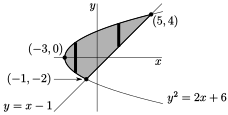
\includegraphics[width=\linewidth]{external/text/figs/areaYvert.pdf}
\end{sbspanel}%
\end{sidebyside}%
\item{}In this region, \(x\) runs from \(a=-3\) to \(b=5\). The curve at the top of the region is%
\begin{align*}
y&=T\big(x)=\sqrt{2x+6}
\end{align*}
The curve at the bottom of the region is more complicated. To the left of \((-1,-2)\) the  lower half of the parabola gives the bottom of the region while to the right of \((-1,-2)\) the straight line gives the bottom of the region. So%
\begin{align*}
B(x)&=\begin{cases}
-\sqrt{2x+6} & \text{if } -3\le x\le -1 \\
x-1 & \text{if }-1\le x\le 5
\end{cases}
\end{align*}
%
\item{}Just as before, the area is still given by the formula \(\int_a^b  \big[T(x)-B(x)\big]\dee{x}\), but to accommodate our \(B(x)\), we have to split up the domain of integration when we evaluate the integral.%
\begin{align*}
& \int_a^b \big[T(x)-B(x)\big]\dee{x}\\
&=  \int_{-3}^{-1} \big[T(x)-B(x)\big]\dee{x}  +\int_{-1}^5 \big[T(x)-B(x)\big]\dee{x}\\
&= \int_{-3}^{-1} \big[\sqrt{2x+6}-(-\sqrt{2x+6})\big]\dee{x}  +\int_{-1}^5 \big[\sqrt{2x+6}-(x-1)\big]\dee{x}\\
&= 2\int_{-3}^{-1} \sqrt{2x+6}\dee{x}  +\int_{-1}^5 \sqrt{2x+6} - \int_{-1}^5(x-1)\dee{x}
\end{align*}
%
\item{}The third integral is straightforward, while we evaluate the first two via the  substitution rule. In particular, set \(u=2x+6\) and replace \(\dee{x} \rightarrow  \frac{1}{2}\dee{u}\). Also \(u(-3)=0, u(-1)=4, u(5)=16\). Hence%
\begin{align*}
\text{Area}
&= 2\int_0^4\sqrt{u}\ \frac{\dee{u}}{2}
+\int_4^{16} \sqrt{u}\ \frac{\dee{u}}{2}
-\int_{-1}^5 (x-1)\dee{x}\\
&= 2\bigg[\frac{ u^{\frac{3}{2}} }{ \frac{3}{2} }\frac{1}{2}\bigg]_0^4
+\bigg[\frac{ u^{\frac{3}{2}} }{ \frac{3}{2} }\frac{1}{2}\bigg]_4^{16}
-\bigg[\frac{x^2}{2}-x\bigg]_{-1}^5\\
& = \frac{2}{3}\big[8-0]
+\frac{1}{3}[64-8]
-\Big[\Big(\frac{25}{2}-5\Big)-\Big(\frac{1}{2}+1\Big)\Big]\\
& = \frac{72}{3} -\frac{24}{2}+6\\
&=18
\end{align*}
Oof!%
\end{itemize}
%
\par
\alert{Easier solution:} The easy way to determine the area of our region is to approximate by narrow  horizontal rectangles, rather than narrow vertical rectangles. (Really we are just  swapping the roles of \(x\) and \(y\) in this problem)%
\begin{itemize}[label=\textbullet]
\item{}Look at our sketch of the region again \textemdash{} each point \((x,y)\) in our  region has \(-2\le y\le 4\) and \(\frac{1}{2}(y^2-6)\le x \le y+1\).%
\item{}Let's use%
\begin{itemize}[label=$\circ$]
\item{}\(c\) to denote the smallest allowed value of \(y\),%
\item{}\(d\) to denote the largest allowed value of \(y\)%
\item{}\(L(y)\) (``\(L\)'' stands for ``left'') to denote the smallest allowed  value of \(x\), when the \(y\)-coordinate is \(y\), and%
\item{}\(R(y)\) (``\(R\)'' stands for ``right'') to denote the largest allowed value  of \(x\), when the \(y\)-coordinate is \(y\).%
\end{itemize}
So, in this example,%
\begin{align*}
c=-2&& d=4 &&  L(y)=\frac{1}{2}(y^2-6) && R(y)=y+1
\end{align*}
and the shaded region is%
\begin{gather*}
\big\{\ (x,y)\ \big|\ c\le y\le d,\ L(y)\le x\le R(y)\ \big\}
\end{gather*}
%
\item{}Our strategy is now nearly the same as that used in Example~\hyperref[example-eg_areabetween_riemann]{{\xreffont\ref{example-eg_areabetween_riemann}}}:%
\begin{itemize}[label=$\circ$]
\item{}Pick a natural number \(n\) (that we will later send to infinity), then%
\item{}subdivide the interval \(c\le y\le d\) into \(n\) narrow subintervals, each of width  \(\De y=\frac{d-c}{n}\). Each subinterval cuts a thin horizontal slice from the region (see  the figure below).%
\item{}We approximate the area of slice number \(i\) by the area of a thin  horizontal rectangle (indicated by the dark rectangle in the figure below). On this  slice, the \(y\)-coordinate runs over a very narrow range.  We pick a number \(y_i^*\), somewhere in that range. We approximate slice  \(i\) by a rectangle whose left side is at \(x=L(y_i^*)\) and whose right side  is at \(x=R(y_i^*)\).%
\item{}Thus the area of slice \(i\) is approximately \(\big[R(x_i^*)-L(x_i^*)\big]\De y\).%
\end{itemize}
%
\begin{sidebyside}{1}{0.1}{0.1}{0}%
\begin{sbspanel}{0.8}%
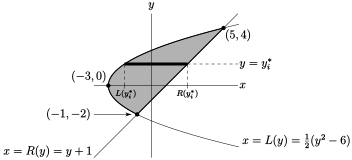
\includegraphics[width=\linewidth]{external/text/figs/areaYhor.pdf}
\end{sbspanel}%
\end{sidebyside}%
\item{}The desired area is%
\begin{align*}
&\lim_{n\rightarrow\infty}\sum_{i=1}^n \big[R(y_i^*)-L(y_i^*)\big]\De y
=\int_c^d \big[R(y)-L(y)\big]\dee{y} \\
&\hskip2in\text{Riemann sum $\rightarrow$ integral}\\
&\hskip1in=\int_{-2}^4 \big[(y+1)-\tfrac{1}{2}\big(y^2-6\big)\big]\dee{y}\\
&=\int_{-2}^4 \big[-\tfrac{1}{2}y^2+y+4\big]\dee{y}\\
&=\Big[-\tfrac{1}{6}y^3+\tfrac{1}{2}y^2+4y\Big]_{-2}^4\\
&=-\tfrac{1}{6}\big(64-(-8)\big)+\tfrac{1}{2}(16-4)+4(4+2)\\
&=-12+6+24\\
&=18
\end{align*}
%
\end{itemize}
%
\end{example}
One last example.%
\begin{example}{Example}{Another area.}{example-eg_AREAc}%
Find the area between the curves \(y=\dfrac{1}{\sqrt{2}}\) and \(y=\sin(x)\) with \(x\) running  from \(0\) to \(\frac{\pi}{2}\).%
\par
\alert{Solution:} This one is a little trickier since (as we shall see) the region is split into two  pieces and we need to treat them separately.%
\par
%
\begin{itemize}[label=\textbullet]
\item{}Again we start by sketching the region.%
\begin{sidebyside}{1}{0.25}{0.25}{0}%
\begin{sbspanel}{0.5}%
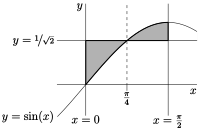
\includegraphics[width=\linewidth]{external/text/figs/areaCross.pdf}
\end{sbspanel}%
\end{sidebyside}%
\par
We want the shaded area.%
\item{}Unlike our previous examples, the bounding curves \(y=\frac{1}{\sqrt{2}}\) and  \(y=\sin(x)\) cross in the middle of the region of interest. They cross when  \(y=\frac{1}{\sqrt{2}}\) and \(\sin(x)=y=\frac{1}{\sqrt{2}}\), i.e. when  \(x=\frac{\pi}{4}\). So%
\begin{itemize}[label=$\circ$]
\item{}to the left of \(x=\frac{\pi}{4}\), the top boundary is part of the straight line  \(y=\frac{1}{\sqrt{2}}\) and  the bottom boundary is part of the curve \(y=\sin(x)\)%
\item{}while to the right of \(x=\frac{\pi}{4}\), the top boundary is part of the curve  \(y=\sin(x)\) and the bottom boundary is part of the straight line  \(y=\frac{1}{\sqrt{2}}\).%
\end{itemize}
%
\item{}Thus the formulae for the top and bottom boundaries are%
\begin{align*}
T(x) & =\left.\begin{cases}
\frac{1}{\sqrt{2}} & \text{if $0\le x\le \frac{\pi}{4}$}\\
\sin(x)& \text{if $\frac{\pi}{4}\le x\le \frac{\pi}{2}$}
\end{cases}\right\}\\
B(x) & =\left.\begin{cases}
\sin(x) & \text{if $0\le x\le \frac{\pi}{4}$}\\
\frac{1}{\sqrt{2}}& \text{if $\frac{\pi}{4}\le x\le \frac{\pi}{2}$}
\end{cases}\right\}
\end{align*}
We may compute the area of interest using our canned formula%
\begin{gather*}
\text{Area} = \int_a^b \big[T(x)-B(x)\big]\dee{x}
\end{gather*}
but since the formulas for \(T(x)\) and \(B(x)\) change at the point \(x=\frac{\pi}{4}\),  we must split the domain of the integral in two at that point \footnotemark{}.%
\item{}Our integral over the domain \(0\leq x \leq \frac{\pi}{2}\) is split into an  integral over \(0\le x\le \frac{\pi}{4}\) and one over \(\frac{\pi}{4}\le x\le  \frac{\pi}{2}\):%
\begin{align*}
\text{Area} &= \int_0^{\frac{\pi}{2}} \big[T(x)-B(x)\big]\dee{x}\\
&= \int_0^{\frac{\pi}{4}} \big[T(x)-B(x)\big]\dee{x} +
\int_{\frac{\pi}{4}}^{\frac{\pi}{2}} \big[T(x)-B(x)\big]\dee{x}\\
&= \int_0^{\frac{\pi}{4}} \Big[\frac{1}{\sqrt{2}}-\sin(x)\Big]\dee{x}
+\int_{\frac{\pi}{4}}^{\frac{\pi}{2}}  \Big[\sin(x)-\frac{1}{\sqrt{2}}\Big]\dee{x}\\
&= \Big[\frac{x}{\sqrt{2}}+\cos(x)\Big]_0^{\frac{\pi}{4}}
+\Big[-\cos(x)-\frac{x}{\sqrt{2}}\Big] _{\frac{\pi}{4}}^{\frac{\pi}{2}}\\
&= \Big[\frac{1}{\sqrt{2}}\frac{\pi}{4}+\frac{1}{\sqrt{2}}-1\Big]
+\Big[\frac{1}{\sqrt{2}}-\frac{1}{\sqrt{2}}\frac{\pi}{4}\Big]\\
&=\frac{2}{\sqrt{2}}-1\\
&=\sqrt{2}-1
\end{align*}
%
\end{itemize}
%
\end{example}
\footnotetext[2]{We are  effectively computing the area of the region by computing the area of the two disjoint  pieces separately. Alternatively, if we set \(f(x) = \sin(x)\) and \(g(x)  =\frac{1}{\sqrt{2}}\), we can rewrite the integral \(\int_a^b \big[T(x) -  B(x)\big]\,\dee{x}\) as \(\int_a^b \big|f(x) - g(x)\big|\,\dee{x}\). To see that the two  integrals are the same, split the domain of integration where \(f(x)-g(x)\) changes sign.\label{fn-eg_AREAc-d-a-c-a-f}}%
\end{subsectionptx}
%
%
\typeout{************************************************}
\typeout{Exercises 1.5.2 Exercises}
\typeout{************************************************}
%
\begin{exercises-subsection}{Exercises}{Exercises}{}{Exercises}{}{}{exercises-sec_area-d}
\par\medskip\noindent%
\textbf{.}\space\space%
\begin{exercisegroup}
\begin{divisionexerciseeg}{1}{}{}{exercise-sec_area-d-a-c}%
We want to approximate the area between the graphs of \(y=\cos x\) and \(y=\sin x\) from \(x=0\) to \(x=\pi\) using a left Riemann sum with \(n=4\) rectangles.%
\begin{enumerate}[label=\alph*]
\item{}On the graph below, sketch the four rectangles.%
\item{}Calculate the Riemann approximation.%
\end{enumerate}
%
\begin{sidebyside}{1}{0.25}{0.25}{0}%
\begin{sbspanel}{0.5}%
\resizebox{\linewidth}{!}{%
\begin{tikzpicture}
\YEaaxis{1}{4.5}{2}{2.25};
\YExcoord{3.14}{\pi}
\YExcoord{1.57}{\frac{\pi}{2}}
\YExcoord{0.79}{\frac{\pi}{4}}
\YExcoord{2.36}{\frac{3\pi}{4}}
\draw[blue, thick] plot[domain=-.5:3.7](\x,{2*cos(\x r)}) node[right]{$y=\cos x$};
\draw[black, thick] plot[domain=-.5:3.7](\x,{2*sin(\x r)}) node[right]{$y=\sin x$};
\end{tikzpicture}
}%
\end{sbspanel}%
\end{sidebyside}%
\end{divisionexerciseeg}%
\begin{divisionexerciseeg}{2}{}{}{exercise-sec_area-d-a-d}%
We want to approximate the bounded area between the curves \(y=\arcsin\left(\dfrac{2x}{\pi}\right)\) and \(y=\sqrt{\dfrac{\pi x}{2}}\) using \(n=5\) rectangles.%
\begin{enumerate}[label=\alph*]
\item{}Draw the five (vertical) rectangles on the picture below corresponding to a right Riemann sum.%
\item{}Draw  five rectangles on the picture below we might use if we were using horizontal rectangles.%
\end{enumerate}
%
\begin{sidebyside}{1}{0.17}{0.17}{0}%
\begin{sbspanel}{0.66}%
\resizebox{\linewidth}{!}{%
\begin{tikzpicture}
\YEaaxis{1.5}{7}{1.5}{6}
\YExcoord{6.28}{\frac{\pi}{2}}
\draw[thick, blue] plot[domain=-.2:1.57, xscale=4, yscale=4]({sin(\x r)/2*3.14},{\x}) ;
\draw[blue] (4,1)node{$y=\arcsin\left(\frac{2x}{\pi}\right)$};
\draw[thick] plot[domain=0:1.8, xscale=4, yscale=4, samples=100]({\x},{sqrt(\x*3.14/2)});
\draw (2,4.75)node{$y=\sqrt{\frac{x\pi}{2}}$};
\end{tikzpicture}
}%
\end{sbspanel}%
\end{sidebyside}%
\end{divisionexerciseeg}%
\begin{divisionexerciseeg}{3}{M121 2002A.}{}{exercise-sec_area-d-a-e}%
Write down a definite integral that represents the finite area bounded by the curves \(y=x^3-x\) and \(y=x\) for \(x\ge 0\). \emph{Do not evaluate the integral explicitly.}%
\end{divisionexerciseeg}%
\begin{divisionexerciseeg}{4}{2000D.}{}{exercise-sec_area-d-a-f}%
Write down a definite integral that represents the area of the region bounded by the line \(y=-\dfrac{x}{2}\) and the parabola \(y^2=6-\dfrac{5x}{4}\). \emph{Do not evaluate the integral explicitly.}%
\end{divisionexerciseeg}%
\begin{divisionexerciseeg}{5}{2001A.}{}{exercise-p1_5_4ax4ay}%
Write down a definite integral that represents the area of the finite plane region bounded by \(y^2=4ax\) and \(x^2=4ay\), where \(a \gt 0\) is a constant. \emph{Do not evaluate the integral explicitly.}%
\end{divisionexerciseeg}%
\begin{divisionexerciseeg}{6}{2001D.}{}{exercise-sec_area-d-a-h}%
Write down a definite integral that represents the area of the region bounded between the line \(x+12y+5=0\) and the curve  \(x=4y^2\). \emph{Do not evaluate the integral explicitly.}%
\end{divisionexerciseeg}%
\end{exercisegroup}
\par\medskip\noindent
\par\medskip\noindent%
\textbf{.}\space\space%
\begin{exercisegroup}
\begin{divisionexerciseeg}{7}{M105 2013A.}{}{exercise-sec_area-d-b-c}%
Find the area of the region bounded by the graph of \(f (x) = \dfrac{1}{(2x-4)^2}\) and the \(x\)-{}-{}axis between \(x = 0\) and \(x = 1\).%
\end{divisionexerciseeg}%
\begin{divisionexerciseeg}{8}{2016Q2.}{}{exercise-sec_area-d-b-d}%
Find the area between the curves \(y=x\) and \(y=3x-x^2\), by first identifying the points of intersection and then integrating.%
\end{divisionexerciseeg}%
\begin{divisionexerciseeg}{9}{2015A.}{}{exercise-sec_area-d-b-e}%
Calculate the area of the region enclosed by \(y = 2^x\) and \(y = \sqrt x+1\).%
\end{divisionexerciseeg}%
\footnotetext[3]{To verify analytically that the curves have no other crossings, write \(f(x)=\sqrt{x}+1-2^x\) and compute \(f'(x)= \frac{1}{2\sqrt{x}}-(\log 2)2^x\). Notice that \(f'(x)\) decreases as \(x\) increases and so can take the value \(0\) for at most a single value of \(x\). Then, by the mean value theorem (or Rolle's theorem, which is Theorem 2.13.1 in the CLP-1 text), \(f(x)\) can take the value \(0\) for at most two distinct values of \(x\).\label{fn-sec_area-d-b-e-e-c-c}}%
\begin{divisionexerciseeg}{10}{2014A.}{}{exercise-sec_area-d-b-f}%
Find the area of the finite region bounded between the two curves \(y = \sqrt{2} \cos(\pi x/4)\) and \(y = |x|\).%
\end{divisionexerciseeg}%
\footnotetext[4]{The solution \(x=1\) was found by guessing. To guess a solution to \(\cos(\pi x/4)=\frac{x}{\sqrt{2}}\) just ask yourself what simple angle has a cosine that involves \(\sqrt{2}\). This guessing strategy is essentially useless in the real world, but works great on problem sets and exams.\label{fn-sec_area-d-b-f-e-c-h}}%
\begin{divisionexerciseeg}{11}{2016Q2.}{}{exercise-sec_area-d-b-g}%
Find the area of the finite region that is bounded by the graphs of \(f(x) = x^2\sqrt{x^3+1}\) and \(g(x) = 3x^2\).%
\end{divisionexerciseeg}%
\begin{divisionexerciseeg}{12}{2016Q2.}{}{exercise-sec_area-d-b-h}%
Find the area to the left of the \(y\)-{}-{}axis and to the right of the curve \(x=y^2+y\).%
\end{divisionexerciseeg}%
\begin{divisionexerciseeg}{13}{}{}{exercise-sec_area-d-b-i}%
Find the area of the finite region  below \(y=\sqrt{9-x^2}\) and above both \(y=|x|\) and \(y=\sqrt{1-x^2}\).%
\end{divisionexerciseeg}%
\end{exercisegroup}
\par\medskip\noindent
\par\medskip\noindent%
\textbf{.}\space\space%
\begin{exercisegroup}
\begin{divisionexerciseeg}{14}{2013A.}{}{exercise-prob_s1_5q5}%
The graph below shows the region between \(y = 4 + \pi \sin x\) and \(y = 4 + 2\pi - 2x\).%
\begin{sidebyside}{1}{0.17}{0.17}{0}%
\begin{sbspanel}{0.66}%
\includegraphics[width=\linewidth]{external/problems/figs/OE13A_4a.pdf}
\end{sbspanel}%
\end{sidebyside}%
\par
Find the area of this region.%
\end{divisionexerciseeg}%
\begin{divisionexerciseeg}{15}{1998A.}{}{exercise-sec_area-d-c-d}%
Compute the area of the finite region bounded by the curves \(x=0\), \(x=3\), \(y=x+2\) and \(y=x^2\).%
\end{divisionexerciseeg}%
\begin{divisionexerciseeg}{16}{2016Q2.}{}{exercise-sec_area-d-c-e}%
Find the total area between the curves \(y = x \sqrt{25-x^2}\) and \(y=3x\), on the interval \(0\le x\le 4\).%
\end{divisionexerciseeg}%
\begin{divisionexerciseeg}{17}{}{}{exercise-sec_area-d-c-f}%
Find the area of the finite region below \(y=\sqrt{9-x^2}\) and \(y=x\), and above  \(y=\sqrt{1-(x-1)^2}\).%
\end{divisionexerciseeg}%
\begin{divisionexerciseeg}{18}{}{}{exercise-sec_area-d-c-g}%
Find the area of the finite region bounded by the curve \(y=x(x^2-4)\) and the line \(y=x-2\).%
\end{divisionexerciseeg}%
\end{exercisegroup}
\par\medskip\noindent
\end{exercises-subsection}
\end{sectionptx}
%
%
\typeout{************************************************}
\typeout{Section 1.6 Volumes}
\typeout{************************************************}
%
\begin{sectionptx}{Section}{Volumes}{}{Volumes}{}{}{section-sec_int_volumes}
\begin{introduction}{}%
Another simple \footnote{Well \textemdash{} arguably the idea isn't too complicated and is a  continuation of the idea used to compute areas in the previous section. In practice this  can be quite tricky as we shall see.\label{fn-sec_int_volumes-b-a-a}} application of integration is computing volumes. We  use the same strategy as we used to express areas of regions in two  dimensions as integrals \textemdash{} approximate the region by a union of small, simple pieces whose volume we can compute and then then take the limit as the ``piece size'' tends to zero.%
\par
In many cases this will lead to ``multivariable integrals'' that are beyond our present  scope \footnote{Typically such integrals (and more) are covered in a third calculus  course.\label{fn-sec_int_volumes-b-b-b}}. But there are some special cases in which this leads to integrals that we  can handle. Here are some examples.%
\begin{example}{Example}{Cone.}{example-eg_VOLa}%
Find the volume of the circular cone of height \(h\) and radius \(r\).%
\par
\alert{Solution:} Here is a sketch of the cone.%
\begin{sidebyside}{1}{0.375}{0.375}{0}%
\begin{sbspanel}{0.25}%
\includegraphics[width=\linewidth]{external/text/figs/cone.pdf}
\end{sbspanel}%
\end{sidebyside}%
\par
We have called the vertical axis \(x\), just so that we end up with a ``\(\dee{x}\)'' integral.%
\par
%
\begin{itemize}[label=\textbullet]
\item{}In what follows we will slice the cone into thin horizontal ``pancakes''. In order  to approximate the volume of those slices, we need to know the radius of the cone at a  height \(x\) above its point. Consider the cross sections shown in the following figure.%
\begin{sidebyside}{1}{0.1}{0.1}{0}%
\begin{sbspanel}{0.8}%
\includegraphics[width=\linewidth]{external/text/figs/cone_adr1.pdf}
\end{sbspanel}%
\end{sidebyside}%
\par
At full height \(h\), the cone has radius \(r\). If we cut the cone at height \(x\), then by  similar triangles (see the figure on the right) the radius will be \(\frac{x}{h}\cdot r\).%
\item{}Now think of cutting the cone into \(n\) thin horizontal ``pancakes''. Each such  pancake is approximately a squat cylinder of height \(\De x=\frac{h}{n}\). This  is very similar to how we approximated the area under a curve by \(n\) tall thin  rectangles. Just as we approximated the area under the curve by summing these rectangles,  we can approximate the volume of the cone by summing the volumes of these cylinders. Here  is a side view of the cone and one of the cylinders.%
\begin{sidebyside}{1}{0.05}{0.05}{0}%
\begin{sbspanel}{0.9}%
\includegraphics[width=\linewidth]{external/text/figs/cone_adr2.pdf}
\end{sbspanel}%
\end{sidebyside}%
\item{}We follow the method we used in Example~\hyperref[example-eg_areabetween_riemann]{{\xreffont\ref{example-eg_areabetween_riemann}}}, except that  our slices are now pancakes instead of rectangles.%
\begin{itemize}[label=$\circ$]
\item{}Pick a natural number \(n\) (that we will later send to infinity), then%
\item{}subdivide the cone into \(n\) thin pancakes, each of width \(\De  x=\frac{h}{n}\).%
\item{}For each \(i=1,2,\cdots,n\), pancake number \(i\) runs from  \(x=x_{i-1}=(i-1)\cdot\De x\) to \(x=x_i=i\cdot\De x\), and we approximate its  volume by the volume of a squat cone. We pick a number \(x_i^*\) between \(x_{i-1}\) and  \(x_i\)  and approximate the pancake by a cylinder of height \(\De x\) and radius \(\frac{x_i^*}{h}r\).%
\item{}Thus the volume of pancake \(i\) is  approximately \(\pi \left( \frac{x_i^*}{h}r\right)^2 \De x\) (as shown in the figure above).%
\end{itemize}
%
\item{}So the Riemann sum approximation of the volume is%
\begin{align*}
\text{Volume} &\approx \sum_{i=1}^n  \pi \left( \frac{x_i^*}{h}r\right)^2 \De x
\end{align*}
%
\item{}By taking the limit as \(n \to \infty\) (i.e. taking the limit as the thickness of  the pancakes goes to zero), we convert the Riemann sum into a definite integral (see  Definition~\hyperref[definition-def_INTintegral]{{\xreffont\ref{definition-def_INTintegral}}}) and at the same time our approximation of the volume  becomes the exact volume:%
\begin{gather*}
\int_0^h \pi \Big(\frac{x}{h}r\Big)^2\dee{x}
\end{gather*}
%
\end{itemize}
Our life \footnotemark{} would be easier if  we could avoid all this formal work with Riemann sums every time we encounter a new  volume. So before we compute the above integral, let us redo the above calculation in a less formal manner.%
\begin{itemize}[label=\textbullet]
\item{}Start again from the picture of the cone%
\begin{sidebyside}{1}{0.375}{0.375}{0}%
\begin{sbspanel}{0.25}%
\includegraphics[width=\linewidth]{external/text/figs/cone.pdf}
\end{sbspanel}%
\end{sidebyside}%
\par
and think of slicing it into thin pancakes, each of width \(\dee{x}\).%
\begin{sidebyside}{2}{0.0425}{0.0425}{0.085}%
\begin{sbspanel}{0.5}[center]%
\includegraphics[width=\linewidth]{external/text/figs/coneX.pdf}
\end{sbspanel}%
\begin{sbspanel}{0.33}[center]%
\includegraphics[width=\linewidth]{external/text/figs/coneT.pdf}
\end{sbspanel}%
\end{sidebyside}%
\item{}The pancake at height \(x\) above the point of the cone (which is the fraction  \(\frac{x}{h}\) of the total height of the cone) has%
\begin{itemize}[label=$\circ$]
\item{}radius \(\frac{x}{h}\cdot r\) (the fraction \(\frac{x}{h}\) of the full radius, \(r\)) and so%
\item{}cross-sectional area \(\pi \big(\frac{x}{h}r\big)^2\),%
\item{}thickness \(\dee{x}\) \textemdash{} we have done something a little sneaky here, see the  discussion below.%
\item{}volume \(\pi \big(\frac{x}{h}r\big)^2\dee{x}\)%
\end{itemize}
As \(x\) runs from \(0\) to \(h\), the total volume is%
\begin{align*}
\int_0^h \pi \Big(\frac{x}{h}r\Big)^2\dee{x}
&=\frac{\pi r^2}{h^2}\int_0^h x^2\dee{x}\\
&=\frac{\pi r^2}{h^2} \bigg[\frac{x^3}{3}\bigg]_0^h\\
&=\frac{1}{3}\pi r^2 h
\end{align*}
%
\end{itemize}
%
\par
In this second computation we are using a time-saving trick. As we saw in  the formal computation above, what we really need to do is pick a natural number \(n\),  slice the cone into \(n\) pancakes each of thickness \(\De x = \frac{h}{n}\) and then  take the limit as \(n \to \infty\). This led to the Riemann sum%
\begin{align*}
\sum_{i=1}^n \pi \left( \frac{x_i^*}{h} r \right)^2 \De x && \text{which becomes}
\int_0^h \pi \left( \frac{x}{h} r \right)^2 \dee{x}
\end{align*}
So knowing that we will replace%
\begin{align*}
\sum_{i=1}^n &\longrightarrow \int_0^h\\
x_i^* &\longrightarrow x\\
\De x &\longrightarrow \dee{x}
\end{align*}
when we take the limit, we have just skipped the intermediate steps. While this is not  entirely rigorous, it can be made so, and does save us a lot of algebra.%
\end{example}
\footnotetext[3]{At least the bits of it involving integrals.\label{fn-eg_VOLa-f-b}}%
\begin{example}{Example}{Sphere.}{example-eg_VOLs}%
Find the volume of the sphere of radius \(r\).%
\par
\alert{Solution:} We'll find the volume of the part of the sphere in the first octant \footnotemark{}, sketched below. Then we'll multiply by \(8\).%
\par
%
\begin{itemize}[label=\textbullet]
\item{}To compute the volume,%
\begin{sidebyside}{1}{0.17}{0.17}{0}%
\begin{sbspanel}{0.66}%
\includegraphics[width=\linewidth]{external/text/figs/sphereSlice.pdf}
\end{sbspanel}%
\end{sidebyside}%
\par
we slice it up into thin vertical ``pancakes'' (just as we did in the previous example).%
\item{}Each pancake is one quarter of a thin circular disk. The pancake a distance \(x\)  from the \(yz\)-plane is shown in the sketch above. The radius of that pancake is the  distance from the dot shown in the figure to the \(x\)-axis, i.e. the \(y\)-coordinate of the dot. To get the coordinates of the dot, observe that%
\begin{itemize}[label=$\circ$]
\item{}it lies the \(xy\)-plane, and so has \(z\)-coordinate zero, and that%
\item{}it also lies on the sphere, so that its coordinates obey  \(x^2+y^2+z^2=r^2\). Since \(z=0\) and \(y \gt 0\), \(y=\sqrt{r^2-x^2}\).%
\end{itemize}
%
\item{}So the pancake at distance \(x\) from the \(yz\)-plane has%
\begin{itemize}[label=$\circ$]
\item{}thickness \footnotemark{} \(\dee{x}\) and%
\item{}radius \(\sqrt{r^2-x^2}\)%
\item{}cross-sectional area \(\frac{1}{4}\pi \big(\sqrt{r^2-x^2}\,\big)^2\)  and hence%
\item{}volume \(\frac{\pi}{4} \big(r^2-x^2\big)\dee{x}\)%
\end{itemize}
%
\item{}As \(x\) runs from \(0\) to \(r\), the total volume of the part of the sphere in the first octant is%
\begin{gather*}
\int_0^r \frac{\pi}{4} \big(r^2-x^2\big)\dee{x}
=\frac{\pi}{4}\bigg[r^2x-\frac{x^3}{3}\bigg]_0^r
=\frac{1}{6}\pi r^3
\end{gather*}
and the total volume of the whole sphere is eight times that, which is \(\frac{4}{3}\pi r^3\), as expected.%
\end{itemize}
%
\end{example}
\footnotetext[4]{The  first octant is the set of all points \((x,y,z)\) with \(x\ge 0\), \(y\ge 0\) and \(z\ge 0\).\label{fn-eg_VOLs-c-b}}%
\footnotetext[5]{Yet again what we really do is pick a natural number \(n\), slice the octant of the sphere into \(n\) pancakes each of thickness  \(\De x=\frac{r}{n}\) and then take the limit \(n\rightarrow\infty\). In the integral \(\De x\) is replaced by \(\dee{x}\). Knowing that this is what is going to happen, we again just skip a few steps.\label{fn-eg_VOLs-d-a-c-a-c-a-a}}%
\begin{example}{Example}{Revolving a region.}{example-eg_VOLe}%
The region between the lines \(y=3\), \(y=5\), \(x=0\) and \(x=4\) is rotated around the line \(y=2\). Find the volume of the region swept out.%
\par
\alert{Solution:} As with most of these problems, we should start by sketching the problem.%
\begin{sidebyside}{1}{0.25}{0.25}{0}%
\begin{sbspanel}{0.5}%
\includegraphics[width=\linewidth]{external/text/figs/revolveA.pdf}
\end{sbspanel}%
\end{sidebyside}%
\par
%
\begin{itemize}[label=\textbullet]
\item{}Consider the region and slice it into thin vertical strips of width  \(\dee{x}\).%
\item{}Now we are to rotate this region about the line \(y=2\). Imagine looking  straight down the axis of rotation, \(y=2\), end on. The symbol in the figure  above just to the right of the end the line \(y=2\) is supposed to represent your  eye \footnotemark{}. Here is what you see as the rotation takes place.%
\begin{sidebyside}{1}{0.25}{0.25}{0}%
\begin{sbspanel}{0.5}%
\includegraphics[width=\linewidth]{external/text/figs/revolveB.pdf}
\end{sbspanel}%
\end{sidebyside}%
\item{}Upon rotation about the line \(y=2\) our strip sweeps out a ``washer''%
\begin{itemize}[label=$\circ$]
\item{}whose cross-section is a disk of radius \(5-2=3\) from which a disk of radius \(3-2=1\) has been removed so that it has a%
\item{}cross-sectional area of \(\pi 3^2 -\pi 1^2 = 8\pi\) and a%
\item{}thickness \(\dee{x}\) and hence a%
\item{}volume \(8\pi\,\dee{x}\).%
\end{itemize}
%
\item{}As our leftmost strip is at \(x=0\) and our rightmost strip is at \(x=4\), the total%
\begin{align*}
\text{Volume} &= \int _0^4 8\pi\,\dee{x} =(8\pi)(4) =32\pi
\end{align*}
%
\end{itemize}
Notice that we could also reach this answer by writing the volume as the difference of two cylinders.%
\begin{itemize}[label=\textbullet]
\item{}The outer cylinder has radius \((5-2)\) and length 4. This has volume%
\begin{align*}
V_{outer} &= \pi r^2 \ell = \pi \cdot 3^2 \cdot 4 = 36\pi.
\end{align*}
%
\item{}The inner cylinder has radius \((3-2)\) and length 4. This has volume%
\begin{align*}
V_{inner} &= \pi r^2 \ell = \pi \cdot 1^2 \cdot 4 = 4\pi.
\end{align*}
%
\item{}The volume we want is the difference of these two, namely%
\begin{align*}
V &= V_{outer} - V_{inner} = 32\pi.
\end{align*}
%
\end{itemize}
%
\end{example}
\footnotetext[6]{Okay okay\textellipsis{} We missed the pupil. I'm sure there is a pun in  there somewhere.\label{fn-eg_VOLe-e-a-b-a-d}}%
Let us turn up the difficulty a little on this last example.%
\begin{example}{Example}{Revolving again.}{example-eg_rot_xaxis}%
The region between the curve \(y=\sqrt{x}\), and the lines \(y=0\), \(x=0\) and \(x=4\) is rotated around the line \(y=0\). Find the volume of the region swept out.%
\par
\alert{Solution:} We can approach this in much the same way as the previous example.%
\begin{itemize}[label=\textbullet]
\item{}Consider the region and cut it into thin vertical strips of width \(\dee{x}\).%
\begin{sidebyside}{1}{0.125}{0.125}{0}%
\begin{sbspanel}{0.75}%
\includegraphics[width=\linewidth]{external/text/figs/rot_rootx1.pdf}
\end{sbspanel}%
\end{sidebyside}%
\item{}When we rotate the region about the line \(y=0\), each strip sweeps out a thin  pancake%
\begin{itemize}[label=$\circ$]
\item{}whose cross-section is a disk of radius \(\sqrt{x}\) with a%
\item{}cross-sectional area of \(\pi (\sqrt{x})^2 = \pi x\) and a%
\item{}thickness \(\dee{x}\) and hence a%
\item{}volume \(\pi x \dee{x}\).%
\end{itemize}
%
\item{}As our leftmost strip is at \(x=0\) and our rightmost strip is at \(x=4\), the total%
\begin{align*}
\text{Volume} &= \int _0^4 \pi x \dee{x} =\left[\frac{\pi}{2}x^2 \right]_0^4 =8\pi
\end{align*}
%
\end{itemize}
%
\end{example}
In the last example we considered rotating a region around the \(x\)-axis. Let us do the same but rotating around the \(y\)-axis.%
\begin{example}{Example}{Revolving yet again.}{example-eg_rot_yaxis}%
The region between the curve \(y=\sqrt{x}\), and the lines \(y=0\), \(x=0\) and \(x=4\) is rotated around the line \(x=0\). Find the volume of the region swept out.%
\par
\alert{Solution:}%
\begin{itemize}[label=\textbullet]
\item{}We will cut the region into horizontal slices, so we should write \(x\) as a  function of \(y\). That is, the region is bounded by \(x=y^2\), \(x=4\), \(y=0\) and \(y=2\).%
\item{}Now slice the region into thin horizontal strips of width \(\dee{y}\).%
\begin{sidebyside}{1}{0.05}{0.05}{0}%
\begin{sbspanel}{0.9}%
\includegraphics[width=\linewidth]{external/text/figs/rot_rootx3.pdf}
\end{sbspanel}%
\end{sidebyside}%
\item{}When we rotate the region about the line \(x=0\), each strip sweeps out a thin  washer%
\begin{itemize}[label=$\circ$]
\item{}whose inner radius is \(y^2\) and outer radius is \(4\), and%
\item{}thickness is \(\dee{y}\) and hence%
\item{}has volume \(\pi(r_{out}^2 - r_{in}^2)\dee{y} = \pi(16-y^4)\dee{y}\).%
\end{itemize}
%
\item{}As our bottommost strip is at \(y=0\) and our topmost  strip is at \(y=2\), the total%
\begin{align*}
\text{Volume}
&= \int _0^2 \pi(16-y^4) \dee{y}
=\left[16\pi y - \frac{\pi}{5}y^5 \right]_0^2
= 32\pi - \frac{32\pi}{5} = \frac{128\pi}{5}.
\end{align*}
%
\end{itemize}
%
\end{example}
There is another way \footnote{The method is not a core part of the course and should be  considered optional.\label{fn-sec_int_volumes-b-j-a}} to do this one which we show at the end of this section.%
\begin{example}{Example}{Pyramid.}{example-eg_VOLb}%
Find the volume of the pyramid which has height \(h\) and whose base is a square of side \(b\).%
\par
\alert{Solution:} Here is a sketch of the part of the pyramid that is in the first octant; we display only this portion to make the diagrams simpler.%
\begin{sidebyside}{2}{0.025}{0.025}{0.05}%
\begin{sbspanel}{0.45}[center]%
\includegraphics[width=\linewidth]{external/text/figs/pyramid.pdf}
\end{sbspanel}%
\begin{sbspanel}{0.45}[center]%
\includegraphics[width=\linewidth]{external/text/figs/pyramidYZ.pdf}
\end{sbspanel}%
\end{sidebyside}%
\par
Note that this diagram shows only 1 quarter of the whole pyramid.%
\par
%
\begin{itemize}[label=\textbullet]
\item{}To compute its volume, we slice it up into thin horizontal ``square pancakes''. A  typical pancake also appears in the sketch above.%
\begin{itemize}[label=$\circ$]
\item{}The pancake at height \(z\) is the fraction \(\frac{h-z}{h}\) of the distance from the  peak of the pyramid to its base.%
\item{}So the \emph{full} pancake \footnotemark{} at height \(z\) is a square of side \(\frac{h-z}{h}b\). As a  check, note that when \(z=h\) the pancake has side  \(\frac{h-h}{h}b=0\), and when \(z=0\) the  pancake has side  \(\frac{h-0}{h}b=b\).%
\item{}So the pancake has cross-sectional area \(\big(\frac{h-z}{h}b\big)^2\) and  thickness \footnotemark{} \(\dee{z}\) and  hence%
\item{}volume \(\big(\frac{h-z}{h}b\big)^2\dee{z}\).%
\end{itemize}
%
\item{}The volume of the whole pyramid (not just the part of the pyramid in the first  octant) is%
\begin{align*}
\int_0^h \Big(\frac{h-z}{h}b\Big)^2\dee{z}
&=\frac{b^2}{h^2} \int_0^h (h-z)^2\dee{z}\\
\intertext{Now use the substitution rule with \(t=(h-z), \dee{z}\to-\dee{t}\)}
&=\frac{b^2}{h^2} \int_h^0 -t^2\dee{t}\\
&=-\frac{b^2}{h^2}\bigg[\frac{t^3}{3}\bigg]_h^0\\
&=-\frac{b^2}{h^2}\bigg[-\frac{h^3}{3}\bigg]\\
&=\frac{1}{3} b^2h
\end{align*}
%
\end{itemize}
%
\end{example}
\footnotetext[8]{Note that this is the full pancake, not just  the part in the first octant.\label{fn-eg_VOLb-f-a-a-a-b-b-b}}%
\footnotetext[9]{We are again using our Riemann sum avoiding trick.\label{fn-eg_VOLb-f-a-a-a-b-c-b}}%
Let's ramp up the difficulty a little.%
\begin{example}{Example}{Napkin Ring.}{example-eg_VOLc}%
Suppose you make two napkin rings \footnotemark{} by drilling holes with different diameters through two  wooden balls. One ball has radius \(r\) and the other radius \(R\) with \(r \lt R\). You  choose the diameter of the holes so that both napkin rings have the same  height, \(2h\). See the figure below.%
\begin{sidebyside}{1}{0.17}{0.17}{0}%
\begin{sbspanel}{0.66}%
\includegraphics[width=\linewidth]{external/text/figs/napkin.pdf}
\end{sbspanel}%
\end{sidebyside}%
\par
Which \footnotemark{} ring has more wood in it?%
\par
\alert{Solution:} We'll compute the volume of the napkin ring with radius \(R\). We can then obtain the volume of the napkin ring of radius \(r\), by just replacing \(R  \mapsto r\) in the result.%
\par
%
\begin{itemize}[label=\textbullet]
\item{}To compute the volume of the napkin ring of radius \(R\), we slice it up into thin  horizontal ``pancakes''. Here is a sketch of the part of the napkin ring in the first octant showing a typical  pancake.%
\begin{sidebyside}{1}{0.17}{0.17}{0}%
\begin{sbspanel}{0.66}%
\includegraphics[width=\linewidth]{external/text/figs/napkinRing.pdf}
\end{sbspanel}%
\end{sidebyside}%
\item{}The coordinates of the two points marked in the \(yz\)-plane of that figure  are found by remembering that%
\begin{itemize}[label=$\circ$]
\item{}the equation of the sphere is \(x^2+y^2+z^2=R^2\).%
\item{}The two points have \(y \gt 0\) and are in the \(yz\)-plane, so that \(x=0\) for them. So \(y=\sqrt{R^2-z^2}\).%
\item{}In particular, at the top of the napkin ring \(z=h\), so that \(y=\sqrt{R^2-h^2}\).%
\end{itemize}
%
\item{}The pancake at height \(z\), shown in the sketch, is a ``washer'' \textemdash{} a circular disk  with a circular hole cut in its center.%
\begin{itemize}[label=$\circ$]
\item{}The outer radius of the washer is \(\sqrt{R^2-z^2}\) and%
\item{}the inner radius of the washer is \(\sqrt{R^2-h^2}\). So the%
\item{}cross-sectional area of the washer is%
\begin{gather*}
\pi\big(\sqrt{R^2-z^2}\,\big)^2-\pi\big(\sqrt{R^2-h^2}\,\big)^2 =\pi(h^2-z^2)
\end{gather*}
%
\end{itemize}
%
\item{}The pancake at height \(z\)%
\begin{itemize}[label=$\circ$]
\item{}has thickness \(dz\) and%
\item{}cross-sectional area \(\pi(h^2-z^2)\) and hence%
\item{}volume \(\pi(h^2-z^2)\dee{z}\).%
\end{itemize}
%
\item{}Since \(z\) runs from \(-h\) to \(+h\), the total volume of wood in the napkin ring of radius \(R\) is%
\begin{align*}
\int_{-h}^h \pi(h^2-z^2)\dee{z}
&=\pi\Big[h^2z-\frac{z^3}{3}\Big]_{-h}^h\\
&=\pi\Big[\Big(h^3-\frac{h^3}{3}\Big)
-\Big((-h)^3-\frac{(-h)^3}{3}\Big)\Big]\\
&=\pi\Big[\frac{2}{3}h^3-\frac{2}{3}\big(-h\big)^3\Big]\\
&=\frac{4\pi}{3}h^3
\end{align*}
%
\end{itemize}
This volume is independent of \(R\). Hence the napkin ring of radius \(r\) contains precisely the same volume of wood as the napkin ring of radius \(R\)!%
\end{example}
\footnotetext[10]{Handy things to have (when combined with cloth  napkins) if your parents are coming to dinner and you want to convince them that you are  ``taking care of yourself''.\label{fn-eg_VOLc-b-a}}%
\footnotetext[11]{A good question to ask to distract your parents from the fact you are  serving frozen burritos.\label{fn-eg_VOLc-d-a}}%
\begin{example}{Example}{Notch.}{example-eg_VOLd}%
A \(45^\circ\) notch is cut to the centre of a cylindrical log having radius \(20\)cm. One plane face of the notch is perpendicular to the axis of the log. See the sketch below. What volume of wood was  removed?%
\begin{sidebyside}{3}{0.0166666666666667}{0.0166666666666667}{0.0333333333333333}%
\begin{sbspanel}{0.3}[center]%
\includegraphics[width=\linewidth]{external/text/figs/notch2.pdf}
\end{sbspanel}%
\begin{sbspanel}{0.3}[center]%
\includegraphics[width=\linewidth]{external/text/figs/notch4a.pdf}
\end{sbspanel}%
\begin{sbspanel}{0.3}[center]%
\includegraphics[width=\linewidth]{external/text/figs/notch5a.pdf}
\end{sbspanel}%
\end{sidebyside}%
\par
\alert{Solution:} We show two solutions to this problem which are of comparable difficulty. The  difference lies in the shape of the pancakes we use to slice up the volume. In solution~1  we cut rectangular pancakes parallel to the \(yz\)-plane and in solution~2 we slice  triangular pancakes parallel to the \(xz\)-plane.%
\par
\emph{Solution 1:}%
\begin{itemize}[label=\textbullet]
\item{}Concentrate on the notch. Rotate it around so that the plane face lies in the  \(xy\)-plane.%
\item{}Then slice the notch into vertical rectangles (parallel to the \(yz\)-plane) as in  the figure on the left below.%
\begin{sidebyside}{2}{0.05}{0.05}{0.1}%
\begin{sbspanel}{0.4}[center]%
\includegraphics[width=\linewidth]{external/text/figs/notch2a.pdf}
\end{sbspanel}%
\begin{sbspanel}{0.4}[center]%
\includegraphics[width=\linewidth]{external/text/figs/notchXZa.pdf}
\end{sbspanel}%
\end{sidebyside}%
\item{}The cylindrical log had radius \(20\)cm. So the circular part of the boundary of the  base of the notch has equation \(x^2+y^2=20^2\). (We're putting the origin of the  \(xy\)-plane at the centre of the circle.) If our coordinate system is such that \(x\) is  constant on each slice, then%
\begin{itemize}[label=$\circ$]
\item{}the base of the slice is the line segment from \((x,-y,0)\) to \((x,+y,0)\) where  \(y=\sqrt{20^2-x^2}\) so that%
\item{}the slice has width \(2y=2\sqrt{20^2-x^2}\) and%
\item{}height \(x\) (since the upper face of the notch is at \(45^\circ\) to the base \textemdash{} see the side view sketched in the figure on the right above).%
\item{}So the slice has cross-sectional area \(2x\sqrt{20^2-x^2}\).%
\end{itemize}
%
\item{}On the base of the notch \(x\) runs from \(0\) to \(20\) so the volume of the notch is%
\begin{align*}
V&=\int_0^{20}2x\sqrt{20^2-x^2}\dee{x}\\
\intertext{Make the change of variables \(u=20^2-x^2\) (don't forget to change \(\dee{x} \rightarrow -\frac{1}{2x}\dee{u}\)):}
V&=\int_{20^2}^{0}-\sqrt{u}\,\dee{u}\\
&=\left[-\frac{u^{3/2}}{3/2}\right]_{20^2}^0\\
&= \frac{2}{3}20^3=\frac{16,000}{3}
\end{align*}
%
\end{itemize}
%
\par
\emph{Solution 2:}%
\begin{itemize}[label=\textbullet]
\item{}Concentrate of the notch. Rotate it around so that its base   lies in the \(xy\)-plane with the skinny edge along the \(y\)-axis.%
\item{}Slice the notch into triangles parallel to the \(xz\)-plane as in the figure  on the left below. In the figure below, the triangle happens to lie in a plane  where \(y\) is negative.%
\begin{sidebyside}{2}{0.05}{0.05}{0.1}%
\begin{sbspanel}{0.4}[center]%
\includegraphics[width=\linewidth]{external/text/figs/notch3a.pdf}
\end{sbspanel}%
\begin{sbspanel}{0.4}[center]%
\includegraphics[width=\linewidth]{external/text/figs/notchXZb.pdf}
\end{sbspanel}%
\end{sidebyside}%
\item{}The cylindrical log had radius \(20\)cm. So the circular part of the boundary of the  base of the notch has equation \(x^2+y^2=20^2\). Our coordinate system is such that \(y\) is  constant on each slice, so that%
\begin{itemize}[label=$\circ$]
\item{}the base of the triangle is the line segment from \((0,y,0)\) to \((x,y,0)\) where   \(x=\sqrt{20^2-y^2}\) so that%
\item{}the triangle has base \(x=\sqrt{20^2-y^2}\)  and%
\item{}height \(x=\sqrt{20^2-y^2}\) (since the upper face of the notch is at  \(45^\circ\) to the base \textemdash{} see the side view sketched in the figure  on the right above).%
\item{}So the slice has cross-sectional area \(\half\big(\sqrt{20^2-y^2}\big)^2\).%
\end{itemize}
%
\item{}On the base of the notch \(y\) runs from \(-20\) to \(20\),  so the volume of the notch is%
\begin{align*}
V&=\half\int_{-20}^{20}(20^2-y^2)\dee{y}\\
&=\int_0^{20} (20^2-y^2)\dee{y}\\
&=\Big[20^2y-\frac{y^3}{3}\Big]_0^{20}\\
&=\frac{2}{3}20^3=\frac{16,000}{3}
\end{align*}
%
\end{itemize}
%
\end{example}
\end{introduction}%
%
%
\typeout{************************************************}
\typeout{Subsection 1.6.1 Optional \textemdash{} Cylindrical shells}
\typeout{************************************************}
%
\begin{subsectionptx}{Subsection}{Optional \textemdash{} Cylindrical shells}{}{Optional \textemdash{} Cylindrical shells}{}{}{subsection-sec_int_volumes-c}
Let us return to Example~\hyperref[example-eg_rot_yaxis]{{\xreffont\ref{example-eg_rot_yaxis}}} in which we rotate a region around the  \(y\)-axis. Here we show another solution to this problem which is obtained by slicing the  region into vertical strips. When rotated about the \(y\)-axis, each such strip sweeps out  a thin cylindrical shell. Hence the name of this approach (and this subsection).%
\begin{example}{Example}{Revolving yet again.}{example-sec_int_volumes-c-c}%
The region between the curve \(y=\sqrt{x}\), and the lines \(y=0\), \(x=0\) and \(x=4\) is rotated around the line \(x=0\). Find the volume of the region swept out.%
\par
\alert{Solution:}%
\begin{itemize}[label=\textbullet]
\item{}Consider the region and cut it into thin vertical strips of width \(\dee{x}\).%
\begin{sidebyside}{1}{0.05}{0.05}{0}%
\begin{sbspanel}{0.9}%
\includegraphics[width=\linewidth]{external/text/figs/rot_rootx2.pdf}
\end{sbspanel}%
\end{sidebyside}%
\item{}When we rotate the region about the line \(y=0\), each strip sweeps out a thin  cylindrical shell%
\begin{itemize}[label=$\circ$]
\item{}whose radius is \(x\),%
\item{}height is \(\sqrt{x}\), and%
\item{}thickness is \(\dee{x}\) and hence%
\item{}has volume \(2 \pi \times \text{radius} \times \text{height} \times \text{thickness}  = 2 \pi x^{3/2} \dee{x}\).%
\end{itemize}
%
\item{}As our leftmost strip is at \(x=0\) and our rightmost strip is at \(x=4\), the total%
\begin{align*}
\text{Volume}
&= \int _0^4 2\pi x^{3/2} \dee{x}
=\left[\frac{4\pi}{5} x^{5/2} \right]_0^4
= \frac{4\pi}{5}\cdot 32 = \frac{128\pi}{5}
\end{align*}
which (thankfully) agrees with our previous computation.%
\end{itemize}
%
\end{example}
\end{subsectionptx}
%
%
\typeout{************************************************}
\typeout{Exercises 1.6.2 Exercises}
\typeout{************************************************}
%
\begin{exercises-subsection}{Exercises}{Exercises}{}{Exercises}{}{}{exercises-sec_int_volumes-d}
\par\medskip\noindent%
\textbf{.}\space\space%
\begin{exercisegroup}
\begin{divisionexerciseeg}{1}{}{}{exercise-sec_int_volumes-d-a-c}%
Consider a right circular cone.%
\begin{sidebyside}{1}{0.375}{0.375}{0}%
\begin{sbspanel}{0.25}%
\resizebox{\linewidth}{!}{%
\begin{tikzpicture}
\draw (0,0)node[thin, gray, shape=ellipse, minimum width=3cm, minimum height=1cm, draw, fill=black, fill opacity=0.1] {};
\draw (-1.5,0)--(0,3)--(1.5,0);
\filldraw[draw=blue, left color=blue!50!black, right color=white, opacity=0.3] (-1.5,0)--(0,3)--(1.5,0) arc(0:-180:1.5cm and 0.5cm);
\end{tikzpicture}
}%
\end{sbspanel}%
\end{sidebyside}%
\par
What shape are horizontal cross-sections? Are the vertical cross-sections the same?%
\end{divisionexerciseeg}%
\begin{divisionexerciseeg}{2}{}{}{exercise-sec_int_volumes-d-a-d}%
Two potters start with a block of clay \(h\) units tall, and identical square cookie cutters. They form columns by pushing the square cookie cutter straight down over the clay, so that its cross-section is the same square as the cookie cutter. Potter A pushes their cookie cutter down while their clay block is sitting motionless on a table; Potter B pushes their cookie cutter down while their clay block is rotating on a potter's wheel, so their column looks twisted. Which column has greater volume?%
\begin{sidebyside}{2}{0.15}{0.15}{0.3}%
\begin{sbspanel}{0.2}%
\resizebox{\linewidth}{!}{%
\begin{tikzpicture}
\draw[thick] (-1.5,-3) --(-0,-3.5)--(1.5,-3)--(1.5,3)--(0,2.5)--(-1.5,3)--cycle;
\draw[thick] (-1.5,3)--(0,3.5)--(1.5,3) (0,2.5)--(0,-3.5);
\fill[bottom color=black, top color=white, fill opacity=0.2] (-1.5,3)--(0,2.5)--(0,-3.5)--(-1.5,-3)--cycle;
\fill[bottom color=blue, top color=white, fill opacity=0.2] (1.5,3)--(0,2.5)--(0,-3.5)--(1.5,-3)--cycle;
 \draw (0,-4.5) node {Column A};
\end{tikzpicture}
}%
\end{sbspanel}%
\begin{sbspanel}{0.2}%
\resizebox{\linewidth}{!}{%
\begin{tikzpicture}
\draw[thick] (-1.5,-3)--(0,-3.5)--(1.5,-3);
\draw[thick] plot[domain=-1.57:1.57]({-1.5*sin(\x r)},1.91*\x);
\draw[thick] (-1.5,3)--(0,2.5)--(1.5,3)--(0,3.5)--cycle;
\draw[thick] plot[domain=-2.1:0, yshift=2.5cm]({-1.25*sin(\x r)},1.91*\x);
\draw[thick] plot[domain=.6:1.57]({1.5*sin(\x r)},1.91*\x);
\draw[thick] plot[domain=-1.57:-.8]({1.5*sin(\x r)},1.91*\x);
\draw[thick] plot[domain=-.75:1.57, yshift=-.5cm]({-1.25*cos(\x r)},-1.91*\x);
\fill[bottom color=black, top color=white, fill opacity=0.5] (0,-3.5)-- plot[domain=-.8:-1.57]({1.5*sin(\x r)},1.91*\x)  plot[domain= .6:1.57, yshift=-.5cm]({-1.25*cos(\x r)},-1.91*\x);
\fill[bottom color=red, top color=white, fill opacity=0.2] (0,2.5) plot[domain=-2.1:0, yshift=2.5cm]({-1.25*sin(\x r)},1.91*\x)--
plot[domain=1.57:-.8]({-1.5*sin(\x r)},1.91*\x)--cycle;
\fill[bottom color=blue, top color=white, fill opacity=0.2] (0,-3.5) --(1.5,-3)
 plot[domain=-1.57:.6]({-1.5*sin(\x r)},1.91*\x)--
plot[domain=-.75:1.57, yshift=-.5cm]({-1.25*cos(\x r)},-1.91*\x);
\fill[bottom color=green!50!blue, top color=white, fill opacity=0.2] (0,2.5) --(1.5,3)
 plot[domain=.6:1.57]({1.5*sin(\x r)},1.91*\x)--(0,2.5)--
 cycle;
 \draw (0,-4.5) node {Column B};
\end{tikzpicture}
}%
\end{sbspanel}%
\end{sidebyside}%
\end{divisionexerciseeg}%
\begin{divisionexerciseeg}{3}{}{}{exercise-sec_int_volumes-d-a-e}%
Let \(R\) be the region bounded above by the graph of \(y=f(x)\) shown below and bounded below by the \(x\)-axis, from \(x=0\) to \(x=6\). Sketch the washers that are formed by rotating \(R\) about the \(y\)-axis. In your sketch, label all the radii in terms of \(y\), and label the thickness.%
\begin{sidebyside}{1}{0.17}{0.17}{0}%
\begin{sbspanel}{0.66}%
\resizebox{\linewidth}{!}{%
\begin{tikzpicture}
\YEaaxis{1}{7}{1}{4}
\draw[ultra thick, blue] (0,0)--(1,1)--(2,0)--(4,3)--(6,0);
\draw[blue](6,1) node  [right]{$y=f(x)$};
\foreach \x in {2,1,4,6}{\YExcoord{\x}{\x}}
\foreach \x in {1,3}{\YEycoord{\x}{\x}}
\draw[dashed] (1,.2)|-(.2,1) (4,.2)|-(.2,3);
\filldraw[blue, opacity=0.1] (0,0)--(1,1)--(2,0)--(4,3)--(6,0)--cycle;
\end{tikzpicture}
}%
\end{sbspanel}%
\end{sidebyside}%
\end{divisionexerciseeg}%
\begin{divisionexerciseeg}{4}{2000D.}{}{exercise-sec_int_volumes-d-a-f}%
Write down definite integrals that represent the following quantities. \emph{Do not evaluate the integrals explicitly.}%
\begin{enumerate}[label=\alph*]
\item{}The volume of the solid obtained by rotating  around the \(x\)-{}-{}axis the region between the \(x\)-{}-{}axis and \(y=\sqrt{x}\, e^{x^2}\) for \(0\le x\le 3\).%
\item{}The volume of the solid obtained by revolving the region bounded by the curves \(y=x^2\) and \(y=x+2\) about the line \(x=3\).%
\end{enumerate}
%
\end{divisionexerciseeg}%
\begin{divisionexerciseeg}{5}{2001A,M121 2001A.}{}{exercise-sec_int_volumes-d-a-g}%
Write down definite integrals that represent the following quantities. \emph{Do not evaluate the integrals explicitly.}%
\begin{enumerate}[label=\alph*]
\item{}The volume of the solid obtained by rotating the finite plane region bounded by the curves \(y=1-x^2\) and \(y=4-4x^2\) about the line \(y=-1\).%
\item{}The volume of the solid obtained by rotating the finite plane region bounded by the curve \(y=x^2-1\) and the line \(y=0\) about the line \(x=5\).%
\end{enumerate}
%
\end{divisionexerciseeg}%
\begin{divisionexerciseeg}{6}{2001D.}{}{exercise-sec_int_volumes-d-a-h}%
Write down a definite integral that represents the volume of the solid obtained by rotating  around the line \(y=-1\) the region between the curves \(y=x^2\) and \(y=8-x^2\). \emph{Do not evaluate the integrals explicitly.}%
\end{divisionexerciseeg}%
\begin{divisionexerciseeg}{7}{}{}{exercise-sec_int_volumes-d-a-i}%
A tetrahedron is a three-dimensional shape with four faces, each of which is an equilateral triangle. (You might have seen this shape as a 4-sided die; think of a pyramid with a triangular base.) Using the methods from this section, calculate the volume of a tetrahedron with side-length \(\ell\). You may assume without proof that the height of a tetrahedron with side-length \(\ell\) is \(\sqrt{\frac{2}{3}}\ell\).%
\begin{sidebyside}{1}{0.3}{0.3}{0}%
\begin{sbspanel}{0.4}%
\resizebox{\linewidth}{!}{%
\begin{tikzpicture}
\draw (0,0) coordinate(a0);
\draw (3,0) coordinate(a1);
\draw (2,-.75) coordinate(a2);
\draw (1.8,2.) coordinate(a3);
\draw[dashed, gray] (a0)--(a1);
\draw[fill, fill opacity=0.3] (a2)--(a3)--(a1)--cycle;
\draw[fill, fill opacity=0.1] (a0)--(a3)--(a2)--cycle;
\draw[decorate, decoration={brace, amplitude=10pt}] (-.2,0.2)--(1.6,2.2) node[midway, above left, xshift=-7pt]{$\ell$};
\draw[decorate, decoration={brace, amplitude=10pt, mirror}] (3.5,0)--(3.5,2) node[midway,  right, xshift=7pt]{$\sqrt{\frac{2}{3}}\ell$};
\end{tikzpicture}
}%
\end{sbspanel}%
\end{sidebyside}%
\end{divisionexerciseeg}%
\end{exercisegroup}
\par\medskip\noindent
\par\medskip\noindent%
\textbf{.}\space\space%
\begin{exercisegroup}
\begin{divisionexerciseeg}{8}{2016Q3.}{}{exercise-sec_int_volumes-d-b-c}%
Let \(a \gt 0\) be a constant. Let \(R\) be the finite region bounded by the graph of \(y=1+\sqrt{x}e^{x^2}\), the line \(y=1\), and the line \(x=a\). Using vertical slices, find the volume generated when \(R\) is rotated about the line \(y=1\).%
\end{divisionexerciseeg}%
\begin{divisionexerciseeg}{9}{2014A.}{}{exercise-sec_int_volumes-d-b-d}%
Find the volume of the solid generated by rotating the finite region bounded by \(y = 1/x\) and \(3x + 3y = 10\) about the \(x\)-{}-{}axis.%
\end{divisionexerciseeg}%
\begin{divisionexerciseeg}{10}{2015A.}{}{exercise-sec_int_volumes-d-b-e}%
Let \(R\) be the region inside the circle \(x^2 + (y-2)^2=1\). Let \(S\) be the solid obtained by rotating \(R\) about the \(x\)-axis.%
\begin{enumerate}[label=\alph*]
\item{}Write down an integral representing the volume of \(S\).%
\item{}Evaluate the integral you wrote down in part (a).%
\end{enumerate}
%
\end{divisionexerciseeg}%
\begin{divisionexerciseeg}{11}{1996D.}{}{exercise-sec_int_volumes-d-b-f}%
The region \(R\) is the portion of the first quadrant which is below the parabola \(y^2=8x\) and above the hyperbola \(y^2-x^2=15\).%
\begin{enumerate}[label=\alph*]
\item{}Sketch the region \(R\).%
\item{}Find the volume of the solid obtained by revolving \(R\) about the \(x\) axis.%
\end{enumerate}
%
\end{divisionexerciseeg}%
\begin{divisionexerciseeg}{12}{1996D.}{}{exercise-sec_int_volumes-d-b-g}%
The region \(R\) is bounded by \(y=\log x\), \(y=0\), \(x=1\) and \(x=2\). (Recall that we are using \(\log x\) to denote the logarithm of \(x\) with base \(e\). In other courses it is often denoted \(\ln x\).)%
\begin{enumerate}[label=\alph*]
\item{}Sketch the region \(R\).%
\item{}Find the volume of the solid obtained by revolving this region  about the \(y\) axis.%
\end{enumerate}
%
\end{divisionexerciseeg}%
\begin{divisionexerciseeg}{13}{2016Q3.}{}{exercise-sec_int_volumes-d-b-h}%
The finite region between the curves \(y = \cos(\frac x2)\) and \(y = x^2 - \pi^2\) is rotated about the line \(y=-{\pi^2}\). Using vertical slices (disks and\slash{}or washers), find the volume of the resulting solid.%
\end{divisionexerciseeg}%
\begin{divisionexerciseeg}{14}{1997D.}{}{exercise-sec_int_volumes-d-b-i}%
The solid \(V\) is 2 meters high and has square horizontal cross sections. The length of the side of the square cross section at height \(x\) meters above the base is \(\frac{2}{1+x}\) m. Find the volume of this solid.%
\end{divisionexerciseeg}%
\begin{divisionexerciseeg}{15}{1998A.}{}{exercise-sec_int_volumes-d-b-j}%
Consider a solid whose base is the finite portion of the \(xy\)-{}-{}plane bounded by the curves \(y=x^2\) and \(y=8-x^2\). The cross-{}-{}sections perpendicular to the \(x\)-{}-{}axis are squares with one side in the \(xy\)-{}-{}plane. Compute the volume of this solid.%
\end{divisionexerciseeg}%
\begin{divisionexerciseeg}{16}{2001D.}{}{exercise-sec_int_volumes-d-b-k}%
A frustrum of a right circular cone (as shown below) has height \(h\). Its base is a circular disc with radius \(4\) and its top is a circular disc with radius \(2\). Calculate the volume of the frustrum.%
\begin{sidebyside}{1}{0.335}{0.335}{0}%
\begin{sbspanel}{0.33}%
\includegraphics[width=\linewidth]{external/problems/figs/OE01D_4b.pdf}
\end{sbspanel}%
\end{sidebyside}%
\end{divisionexerciseeg}%
\end{exercisegroup}
\par\medskip\noindent
\par\medskip\noindent%
\textbf{.}\space\space%
\begin{exercisegroup}
\begin{divisionexerciseeg}{17}{}{}{exercise-sec_int_volumes-d-c-c}%
The shape of the earth is often approximated by an oblate spheroid, rather than a sphere. An \emph{oblate spheroid} is formed by rotating an ellipse about its \emph{minor axis} (its shortest diameter).%
\begin{enumerate}[label=\alph*]
\item{}Find the volume of the oblate spheroid obtained by rotating the upper (positive) half of the ellipse \((ax)^2+(by)^2=1\) about the \(x\)-axis, where \(a\) and \(b\) are positive constants with \(a \geq b\).%
\item{}Suppose \footnotemark{} the earth has radius at the equator of 6378.137  km, and radius at the poles of 6356.752 km. If we model the earth as an oblate spheroid formed by rotating the upper half of the ellipse \((ax)^2+(by)^2=1\) about the \(x\)-axis, what are \(a\) and \(b\)?%
\item{}What is the volume of this model of the earth? (Use a calculator.)%
\item{}Suppose we had calculated the volume of the earth by modelling it as a sphere with radius \(6378.137\) km. What would our absolute and relative errors be, compared to our oblate spheroid calculation?%
\end{enumerate}
%
\end{divisionexerciseeg}%
\footnotetext[12]{\href{https://nssdc.gsfc.nasa.gov/planetary/factsheet/earthfact.html}{Earth Fact Sheet}\footnotemark{}, NASA, accessed 2 July 2017\label{fn-sec_int_volumes-d-c-c-a-a-c-b-a}}%
\footnotetext[13]{\nolinkurl{nssdc.gsfc.nasa.gov/planetary/factsheet/earthfact.html}\label{fn-sec_int_volumes-d-c-c-a-a-c-b-a-b}}%
\begin{divisionexerciseeg}{18}{2012A.}{}{exercise-sec_int_volumes-d-c-d}%
Let \(R\) be the bounded region that lies between the curve \(y = 4 - (x - 1)^2\) and the line \(y = x + 1\).%
\begin{enumerate}[label=\alph*]
\item{}Sketch \(R\) and find its area.%
\item{}Write down a definite integral giving the volume of the region obtained by rotating \(R\) about the line \(y = 5\). \emph{Do not evaluate this integral.}%
\end{enumerate}
%
\end{divisionexerciseeg}%
\begin{divisionexerciseeg}{19}{M121 1999A.}{}{exercise-sec_int_volumes-d-c-e}%
Let \(\cR=\big\{(x,y)\ :\ (x-1)^2+y^2\le 1\text{
and } x^2+(y-1)^2\le 1\ \big\}\).%
\begin{enumerate}[label=\alph*]
\item{}Sketch \(\cR\) and find its area.%
\item{}If \(\cR\) rotates around the \(y\)-{}-{}axis, what volume is generated?%
\end{enumerate}
%
\end{divisionexerciseeg}%
\begin{divisionexerciseeg}{20}{1997A.}{}{exercise-sec_int_volumes-d-c-f}%
Let \(\cR\) be the plane region bounded by \(x=0,\ x=1,\ y=0\) and \(y=c\sqrt{1+x^2}\), where \(c\ge 0\) is a constant.%
\begin{enumerate}[label=\alph*]
\item{}Find the volume \(V_1\) of the solid obtained by revolving \(\cR\) about the \(x\)-{}-{}axis.%
\item{}Find the volume \(V_2\) of the solid obtained by revolving \(\cR\) about the \(y\)-{}-{}axis.%
\item{}If \(V_1=V_2\), what is the value of \(c\)?%
\end{enumerate}
%
\end{divisionexerciseeg}%
\begin{divisionexerciseeg}{21}{2013A.}{}{exercise-sec_int_volumes-d-c-g}%
The graph below shows the region between \(y = 4 + \pi \sin x\) and \(y = 4 + 2\pi - 2x\).%
\begin{sidebyside}{1}{0.17}{0.17}{0}%
\begin{sbspanel}{0.66}%
\includegraphics[width=\linewidth]{external/problems/figs/OE13A_4a.pdf}
\end{sbspanel}%
\end{sidebyside}%
\par
The region is rotated about the line \(y = -1\). Express in terms of definite integrals the volume of the resulting solid. Do not evaluate the integrals.%
\end{divisionexerciseeg}%
\begin{divisionexerciseeg}{22}{}{}{exercise-prob_s1_6_density}%
On a particular, highly homogeneous \footnotemark{} planet, we observe that the density of the atmosphere \(h\) kilometres above the surface is given by the equation \(\rho(h) = c2^{-h/6}\quad \frac{\mathrm{kg}}{\mathrm{m^3}}\), where \(c\) is the density on the planet's surface.%
\begin{enumerate}[label=\alph*]
\item{}What is the mass of the atmosphere contained in a vertical column with radius one metre,  sixty kilometres high?%
\item{}What height should a column be to contain \(\dfrac{3000c\pi}{\log 2}\) kilograms of air?%
\end{enumerate}
%
\end{divisionexerciseeg}%
\footnotetext[14]{This is clearly a simplified model: air density changes all the time, and depends on lots of complicated factors aside from altitude. However, the equation we're using is not so far off from an idealized model of the earth's atmosphere, taken from \href{http://www.indiana.edu/\~geog109/topics/10_Forces\%26Winds/GasPressWeb/PressGasLaws.html}{Pressure and the Gas Laws}\footnotemark{} by H.P. Schmid, accessed 3 July 2017.\label{fn-prob_s1_6_density-a-a-a}}%
\footnotetext[15]{\nolinkurl{www.indiana.edu/\~geog109/topics/10_Forces\%26Winds/GasPressWeb/PressGasLaws.html}\label{fn-prob_s1_6_density-a-a-a-b}}%
\end{exercisegroup}
\par\medskip\noindent
\end{exercises-subsection}
\end{sectionptx}
%
%
\typeout{************************************************}
\typeout{Section 1.7 Integration by parts}
\typeout{************************************************}
%
\begin{sectionptx}{Section}{Integration by parts}{}{Integration by parts}{}{}{section-sec_intbyparts}
\begin{introduction}{}%
\end{introduction}%
%
%
\typeout{************************************************}
\typeout{Subsection 1.7.1 Integration by parts}
\typeout{************************************************}
%
\begin{subsectionptx}{Subsection}{Integration by parts}{}{Integration by parts}{}{}{subsection-sec_intbyparts-c}
The fundamental theorem of calculus tells us that it is very easy to integrate a  derivative. In particular, we know that%
\begin{align*}
\int \diff{}{x}\left( F(x) \right) \dee{x} &= F(x)+C
\end{align*}
We can exploit this in order to develop another rule for integration \textemdash{} in particular a  rule to help us integrate products of simpler function such as%
\begin{gather*}
\int x e^x \dee{x}
\end{gather*}
In so doing we will arrive at a method called ``integration by parts''.%
\par
To do this we start with the product rule and integrate. Recall that the  product rule says%
\begin{gather*}
\diff{}{x} u(x)v(x) = u'(x)\,v(x)+u(x)\,v'(x)
\end{gather*}
Integrating this gives%
\begin{align*}
\int \big[u'(x)\,v(x)+u(x)\,v'(x)\big]\dee{x}
&=\big[\text{a function whose derivative is $u'v+uv'$}\big] + C\\
&=u(x)v(x) +C
\end{align*}
Now this, by itself, is not terribly useful. In order to apply it we need to have a  function whose integrand is a sum of products that is in exactly this form \(u'(x)v(x) +  u(x)v'(x)\). This is far too specialised.%
\par
However if we tease this apart a little:%
\begin{align*}
\int \big[ u'(x)\,v(x) + u(x)\,v'(x) \big]\dee{x}
&=  \int u'(x)\,v(x) \,\dee{x}
+\int u(x)\,v'(x) \,\dee{x}\\
\intertext{Bring one of the integrals to the left-hand side}
u(x) v(x) - \int u'(x)\,v(x) \dee{x}
&= \int u(x)\,v'(x)\dee{x}\\
\intertext{Swap left and right sides}
\int u(x)\,v'(x)\dee{x}
&= u(x) v(x) - \int u'(x)\,v(x) \dee{x}
\end{align*}
In this form we take the integral of one product and express it in terms of the integral  of a different product. If we express it like that, it doesn't seem too useful. However,  if the second integral is easier, then this process helps us.%
\par
Let us do a simple example before explaining this more generally.%
\begin{example}{Example}{\(\int xe^x \dee{x}\).}{example-eg_PRTSxex}%
Compute the integral \(\ds \int xe^x \dee{x}\).%
\par
\alert{Solution:}%
\begin{itemize}[label=\textbullet]
\item{}We start by taking the equation above%
\begin{align*}
\int u(x)\,v'(x)\dee{x}
&= u(x) v(x) - \int u'(x)\,v(x) \dee{x}
\end{align*}
%
\item{}Now set \(u(x)=x\) and \(v'(x)=e^x\). How did we know how to make this choice? We will  explain some strategies later. For now, let us just accept this choice and keep going.%
\item{}In order to use the formula we need to know \(u'(x)\) and \(v(x)\). In this case it is  quite straightforward: \(u'(x)=1\) and \(v(x)=e^x\).%
\item{}Plug everything into the formula:%
\begin{align*}
\int x e^x \dee{x} &= x e^x - \int e^x \dee{x}\\
\intertext{So our original more difficult integral has been turned into a question of  computing an easy one.}
&= x e^x - e^x +C
\end{align*}
%
\item{}We can check our answer by differentiating:%
\begin{align*}
\diff{}{x} \left(x e^x - e^x +C \right)
&= \underbrace{x e^x + 1 \cdot e^x}_{\text{by product rule}} - e^x + 0\\
&= x e^x & \text{as required.}
\end{align*}
%
\end{itemize}
%
\end{example}
The process we have used in the above example is called ``integration by parts''. When  our integrand is a product we try to write it as \(u(x) v'(x)\) \textemdash{} we need to choose one  factor to be \(u(x)\) and the other to be \(v'(x)\). We then compute \(u'(x)\) and \(v(x)\) and  then apply the following theorem:%
\begin{theorem}{Theorem}{Integration by parts.}{}{theorem-thm_PRTSintbyparts}%
Let \(u(x)\) and \(v(x)\) be continuously differentiable. Then%
\begin{gather*}
\int u(x)\,v'(x)\dee{x} = u(x)\,v(x)-\int v(x)\,u'(x)\dee{x}
\end{gather*}
If we write \(\dee{v}\) for \(v'(x)\dee{x}\) and \(\dee{u}\) for \(u'(x)\dee{x}\) (as the substitution rule  suggests), then the formula becomes%
\begin{gather*}
\int u\dee{v}= u\,v-\int v\dee{u}
\end{gather*}
The application of this formula is known as integration by parts.%
\par
The corresponding statement for definite integrals is%
\begin{gather*}
\int_a^b u(x)\,v'(x)\dee{x} = u(b)\,v(b)-u(a)\,v(a)-\int_a^b v(x)\,u'(x)\dee{x}
\end{gather*}
%
\end{theorem}
Integration by parts is not as easy to apply as the product rule for derivatives. This is  because it relies on us%
\begin{enumerate}[label=\arabic*]
\item{}judiciously choosing \(u(x)\) and \(v'(x)\), then%
\item{}computing \(u'(x)\) and \(v(x)\) \textemdash{} which requires us to  antidifferentiate \(v'(x)\), and finally%
\item{}that the integral \(\int u'(x) v(x)\dee{x}\) is easier than the integral we started  with.%
\end{enumerate}
%
\par
Notice that any antiderivative of \(v'(x)\) will do. All antiderivatives of  \(v'(x)\) are of the form \(v(x)+A\) with \(A\) a constant. Putting this into the  integration by parts formula gives%
\begin{align*}
\int u(x) v'(x)\dee{x} &= u(x) \left( v(x)+A \right) - \int u'(x)\left(  v(x)+A\right) \dee{x}\\
&= u(x)v(x) + A u(x) - \int u'(x) v(x) \dee{x}- \underbrace{A \int u'(x)  \dee{x}}_{= A u(x) + C}\\
&= u(x)v(x) - \int u'(x) v(x)\dee{x}  + C
\end{align*}
So that constant \(A\) will always cancel out.%
\par
In most applications (but not all) our integrand will be a product of two factors so we  have two choices for \(u(x)\) and \(v'(x)\). Typically one of these choices will be ``good''  (in that it results in a simpler integral) while the other will be ``bad'' (we cannot  antidifferentiate our choice of \(v'(x)\) or the resulting integral is harder). Let us  illustrate what we mean by returning to our previous example.%
\begin{example}{Example}{\(\int xe^x \dee{x}\) \textemdash{} again.}{example-sec_intbyparts-c-l}%
Our integrand is the product of two factors%
\begin{align*}
x && \text{and} && e^x
\end{align*}
This gives us two obvious choices of \(u\) and \(v'\):%
\begin{align*}
u(x)&=x & v'(x)&=e^x\\
\text{ or}\\
u(x)&=e^x & v'(x)&=x
\end{align*}
We should explore both choices:%
\begin{enumerate}
\item{}If take \(u(x)=x\) and \(v'(x)=e^x\). We then quickly compute%
\begin{align*}
u'(x)&=1 &\text{and} && v(x)=e^x
\end{align*}
which means we will need to integrate (in the right-hand side of the integration by  parts formula)%
\begin{align*}
\int u'(x) v(x) \dee{x} &= \int 1 \cdot e^x \dee{x}
\end{align*}
which looks straightforward. This is a good indication that this is the right choice of \(u(x)\) and \(v'(x)\).%
\item{}But before we do that, we should also explore the other choice, namely \(u(x)=e^x\)  and \(v'(x)=x\). This implies that%
\begin{align*}
u'(x)&= e^x &\text{and}&& v(x)&= \frac{1}{2}x^2
\end{align*}
which means we need to integrate%
\begin{align*}
\int u'(x) v(x) \dee{x} &= \int \frac{1}{2}x^2 \cdot e^x \dee{x}.
\end{align*}
This is at least as hard as the integral we started with. Hence we should try the first  choice.%
\end{enumerate}
With our choice made, we integrate by parts to get%
\begin{align*}
\int xe^x \dee{x} &= xe^x - \int e^x \dee{x}\\
&= xe^x - e^x +C.
\end{align*}
The above reasoning is a very typical workflow when using integration by  parts.%
\end{example}
Integration by parts is often used%
\begin{itemize}[label=\textbullet]
\item{}to eliminate factors of \(x\) from an integrand like \(xe^x\) by using that  \(\diff{}{x}x=1\) and%
\item{}to eliminate a \(\log x\) from an integrand by using that \(\diff{}{x}\log x=\frac{1}{x}\) and%
\item{}to eliminate inverse trig functions, like \(\arctan x\), from an integrand by using that, for example, \(\diff{}{x}\arctan x=\frac{1}{1+x^2}\).%
\end{itemize}
%
\begin{example}{Example}{\(\int x\sin x\dee{x}\).}{example-sec_intbyparts-c-n}%
\alert{Solution:}%
\begin{itemize}[label=\textbullet]
\item{}Again we have a product of two factors giving us two possible choices.%
\begin{enumerate}[label=\arabic*]
\item{}If we choose \(u(x)=x\) and \(v'(x)=\sin x\), then we get%
\begin{align*}
u'(x) &=1 &\text{and} && v(x) &= -\cos x
\end{align*}
which is looking promising.%
\item{}On the other hand if we choose \(u(x)=\sin x\) and \(v'(x)=x\), then we have%
\begin{align*}
u'(x)&=\cos x &\text{and} && v(x) &= \frac{1}{2}x^2
\end{align*}
which is looking worse \textemdash{} we'd need to integrate \(\int \frac{1}{2}x^2 \cos x \dee{x}\).%
\end{enumerate}
%
\item{}So we stick with the first choice. Plugging \(u(x)=x\), \(v(x)=-\cos x\)  into  integration by parts gives us%
\begin{align*}
\int x \sin x \dee{x} &= -x\cos x  - \int 1 \cdot (-\cos x) \dee{x}\\
&= -x\cos x + \sin x + C
\end{align*}
%
\item{}Again we can check our answer by differentiating:%
\begin{align*}
\diff{}{x}\left( -x\cos x + \sin x + C \right)
&= -\cos x + x\sin x + \cos x + 0\\
&= x \sin x \checkmark
\end{align*}
%
\end{itemize}
%
\par
Once we have practised this a bit we do not really need to write as much. Let us solve it  again, but showing only what we need to.%
\par
\alert{Solution:}%
\begin{itemize}[label=\textbullet]
\item{}We use integration by parts to solve the integral.%
\item{}Set \(u(x)=x\) and \(v'(x)=\sin x\). Then \(u'(x)=1\) and \(v(x)=-\cos x\), and%
\begin{align*}
\int x \sin x \dee{x} &= -x\cos x + \int \cos x \dee{x}\\
&= -x\cos x + \sin x + C.
\end{align*}
%
\end{itemize}
%
\end{example}
It is pretty standard practice to reduce the notation even further in these  problems. As noted above, many people write the integration by parts formula as%
\begin{align*}
\int u\dee{v} &= uv - \int v \dee{u}
\end{align*}
where \(\dee{u}, \dee{v}\) are shorthand for \(u'(x)\dee{x}, v'(x)\dee{x}\). Let us  write up the previous example using this notation.%
\begin{example}{Example}{\(\int x\sin x\dee{x}\) yet again.}{example-eg_PRTSxsinx}%
\alert{Solution:} Using integration by parts, we set \(u=x\) and \(\dee{v}=\sin x\dee{x}\). This makes  \(\dee{u}= 1\dee{x}\) and \(v=-\cos x\). Consequently%
\begin{align*}
\int x \sin x \dee{x} &= \int u\dee{v}\\
&= uv - \int v\dee{u}\\
&= -x\cos x + \int \cos x \dee{x}\\
&= -x \cos x +\sin x + C
\end{align*}
You can see that this is a very neat way to write up these problems and we will  continue using this shorthand in the examples that follow below.%
\end{example}
We can also use integration by parts to eliminate higher powers of \(x\). We just  need to apply the method more than once.%
\begin{example}{Example}{\(\int x^2 e^x \dee{x}\).}{example-eg_PRTSxtwoex}%
\alert{Solution:}%
\begin{itemize}[label=\textbullet]
\item{}Let \(u=x^2\) and \(\dee{v}=e^x\dee{x}\). This then gives  \(\dee{u}=2x\dee{x}\) and \(v=e^x\), and%
\begin{align*}
\int x^2 e^x \dee{x} &= x^2 e^x - \int 2x e^x \dee{x}
\end{align*}
%
\item{}So we have reduced the problem of computing the original integral to one of  integrating \(2xe^x\). We know how to do this \textemdash{} just integrate by parts again:%
\begin{align*}
\int x^2 e^x \dee{x} &= x^2 e^x - \int 2x e^x \dee{x}
& \text{set $u=2x, \dee{v}=e^x\dee{x}$}\\
&= x^2 e^x - \left( 2xe^x - \int 2 e^x \dee{x} \right)
& \text{since $\dee{u}=2\dee{x}, v=e^x$}\\
&= x^2 e^x - 2xe^x + 2e^x + C
\end{align*}
%
\item{}We can, if needed, check our answer by differentiating:%
\begin{align*}
&\diff{}{x} \left( x^2 e^x - 2xe^x + 2e^x + C \right)\\
&\hskip1in= \left( x^2 e^x + 2xe^x \right) - \left(2x e^x + 2e^x \right) + 2e^x + 0\\
&\hskip1in= x^2 e^x \checkmark
\end{align*}
%
\end{itemize}
A similar iterated application of integration by parts will work for integrals%
\begin{gather*}
\int P(x) \left(Ae^{ax} + B\sin(bx) + C\cos(cx) \right) \dee{x}
\end{gather*}
where \(P(x)\) is a polynomial and \(A,B,C,a,b,c\) are constants.%
\end{example}
Now let us look at integrands containing logarithms. We don't know the antiderivative of  \(\log x\), but we can eliminate \(\log x\) from an integrand by using integration by parts  with \(u=\log x\). Remember \(\log x = \log_e x = \ln x\).%
\begin{example}{Example}{\(\int x\log x\dee{x}\).}{example-eg_PRTSxlnx}%
\alert{Solution:}%
\begin{itemize}[label=\textbullet]
\item{}We have two choices for \(u\) and \(\dee{v}\).%
\begin{enumerate}[label=\arabic*]
\item{}Set \(u=x\) and \(\dee{v}=\log x\dee{x}\). This gives \(\dee{u}=\dee{x}\) but  \(v\) is hard to compute \textemdash{} we haven't done it yet \footnotemark{}. Before we go further along this path, we should look to see what happens with the other choice.%
\item{}Set \(u=\log x\) and \(\dee{v}=x\dee{x}\). This gives  \(\dee{u}=\frac{1}{x}\dee{x}\) and \(v=\frac{1}{2}x^2\), and we have to integrate%
\begin{align*}
\int v\, \dee{u} &= \int \frac{1}{x} \cdot \frac{1}{2}x^2 \dee{x}
\end{align*}
which is easy.%
\end{enumerate}
%
\item{}So we proceed with the second choice.%
\begin{align*}
\int x \log x \dee{x}
&= \frac{1}{2}x^2 \log x - \int \frac{1}{2} x \dee{x}\\
&= \frac{1}{2}x^2 \log x - \frac{1}{4}x^2 +C
\end{align*}
%
\item{}We can check our answer quickly:%
\begin{align*}
\diff{}{x} \Big(\frac{x^2}{2} \ln x -\frac{x^2}{4} +C\Big)
&= x\,\ln x + \frac{x^2}{2}\,\frac{1}{x} -\frac{x}{2}+0
=x\,\ln x
\end{align*}
%
\end{itemize}
%
\end{example}
\footnotetext[1]{We will soon.\label{fn-eg_PRTSxlnx-b-b-a-a-c-a-f}}%
\begin{example}{Example}{\(\int \log x\dee{x}\).}{example-eg_PRTSlnx}%
It is not immediately obvious that one should use integration by parts to  compute the integral%
\begin{gather*}
\int \log x \dee{x}
\end{gather*}
since the integrand is not a product. But we should persevere \textemdash{} indeed this  is a situation where our shorter notation helps to clarify how to proceed.%
\par
\alert{Solution:}%
\begin{itemize}[label=\textbullet]
\item{}In the previous example we saw that we could remove the factor \(\log x\) by  setting \(u=\log x\) and using integration by parts. Let us try repeating  this. When we make this choice, we are then forced to take \(\dee{v}=\dee{x}\)  \textemdash{} that is we choose \(v'(x)=1\). Once we have made this sneaky move everything  follows quite directly.%
\item{}We then have \(\dee{u} = \frac{1}{x}\dee{x}\) and \(v = x\), and the  integration by parts formula gives us%
\begin{align*}
\int \log x \dee{x}
&= x \log x - \int \frac{1}{x} \cdot x \dee{x}\\
&= x\log x - \int 1 \dee{x}\\
&= x \log x - x + C
\end{align*}
%
\item{}As always, it is a good idea to check our result by verifying that the derivative of the answer really is the integrand.%
\begin{align*}
\diff{}{x} \big(x\ln x-x +C\big) &= \ln x + x\,\frac{1}{x} -1+0 =\ln x
\end{align*}
%
\end{itemize}
%
\end{example}
The same method works almost exactly to compute the antiderivatives of  \(\arcsin(x)\) and \(\arctan(x)\):%
\begin{example}{Example}{\(\int \arctan(x)\dee{x}\) and \(\int \arcsin(x)\dee{x}\).}{example-eg_invtan}%
Compute the antiderivatives of the inverse sine and inverse tangent functions.%
\par
\alert{Solution:}%
\begin{itemize}[label=\textbullet]
\item{}Again neither of these integrands are products, but that is no  impediment. In both cases we set \(\dee{v}=\dee{x}\) (ie \(v'(x)=1\)) and choose \(v(x)=x\).%
\item{}For inverse tan we choose \(u=\arctan(x)\), so  \(\dee{u}=\frac{1}{1+x^2}\dee{x}\):%
\begin{align*}
\int \arctan(x) \dee{x}
&= x \arctan(x) - \int x \cdot \frac{1}{1+x^2} \dee{x}\\
\intertext{now use substitution rule with \(w(x)=1+x^2, w'(x)=2x\)}
&= x \arctan(x) - \int \frac{w'(x)}{2} \cdot \frac{1}{w} \dee{x}\\
&= x \arctan(x) - \frac{1}{2} \int \frac{1}{w} \dee{w}\\
&= x \arctan(x) - \frac{1}{2}\log |w| + C\\
&= x \arctan(x) - \frac{1}{2} \log|1+x^2| + C \qquad \text{but $1+x^2 \gt 0$, so}\\
&= x \arctan(x) - \frac{1}{2} \log(1+x^2) + C
\end{align*}
%
\item{}Similarly for inverse sine we choose \(u=\arcsin(x)\) so \(\dee{u} =  \frac{1}{\sqrt{1-x^2}}\dee{x}\):%
\begin{align*}
\int \arcsin(x) \dee{x}
&= x \arcsin(x) - \int \frac{x}{\sqrt{1-x^2}} \dee{x}\\
\intertext{Now use substitution rule with \(w(x)=1-x^2, w'(x)=-2x\)}
&= x \arcsin(x) - \int \frac{-w'(x)}{2} \cdot w^{-1/2} \dee{x}\\
&= x\arcsin(x) + \frac{1}{2} \int w^{-1/2} \dee{w}\\
&= x \arcsin(x) + \frac{1}{2} \cdot 2 w^{1/2} + C\\
&= x\arcsin(x) + \sqrt{1-x^2} + C
\end{align*}
%
\item{}Both can be checked quite quickly by differentiating \textemdash{} but we leave  that as an exercise for the reader.%
\end{itemize}
%
\end{example}
There are many other examples we could do, but we'll finish with a tricky one.%
\begin{example}{Example}{\(\int e^x \sin x\dee{x}\).}{example-eg_circularint}%
\alert{Solution:} Let us attempt this one a little naively and then we'll come back and do  it more carefully (and successfully).%
\begin{itemize}[label=\textbullet]
\item{}We can choose either \(u=e^x, \dee{v}=\sin x\dee{x}\) or the other way  around.%
\begin{enumerate}
\item{}Let \(u=e^x, \dee{v}=\sin x\dee{x}\). Then \(\dee{u}=e^x\dee{x}\) and  \(v=-\cos x\). This gives%
\begin{align*}
\int e^x \sin x &= -e^x\cos x + \int e^x \cos x \dee{x}
\end{align*}
So we are left with an integrand that is very similar to the one  we started with. What about the other choice?%
\item{}Let \(u=\sin x, \dee{v}=e^x\dee{x}\). Then \(\dee{u}=\cos x\dee{x}\) and  \(v= e^x\). This gives%
\begin{align*}
\int e^x \sin x &= e^x\sin x - \int e^x \cos x \dee{x}
\end{align*}
So we are again left with an integrand that is very similar to the one  we started with.%
\end{enumerate}
%
\item{}How do we proceed? \textemdash{} It turns out to be easier if you do both \(\int  e^x\sin x\dee{x}\) and \(\int e^x \cos x\dee{x}\) simultaneously. We do so in the  next example.%
\end{itemize}
%
\end{example}
\begin{example}{Example}{\(\int_a^b e^x\sin x\dee{x}\) and \(\int_a^b e^x\cos x\dee{x}\).}{example-eg_PRTSexsinx}%
This time we're going to do the two integrals%
\begin{align*}
I_1&=\int_a^b e^x\sin x\dee{x}
&
I_2 &=\int_a^b e^x\cos x\dee{x}
\end{align*}
at more or less the same time.%
\par
%
\begin{itemize}[label=\textbullet]
\item{}First%
\begin{align*}
I_1=\int_a^b e^x\sin x\dee{x}
&=\int_a^b u \dee{v} \qquad\\
\intertext{Choose \(u=e^x, \dee{v} = \sin x\dee{x}\), so \(v = -\cos x, \dee{u}= e^x\dee{x}\)}
&=\Big[-e^x\cos x\Big]_a^b +\int_a^b e^x\cos x\dee{x}
\end{align*}
We have not found \(I_1\) but we have related it to \(I_2\).%
\begin{align*}
I_1&=\Big[-e^x\cos x\Big]_a^b +I_2
\end{align*}
%
\item{}Now start over with \(I_2\).%
\begin{align*}
I_2=\int_a^b e^x\cos x\dee{x}
&=\int_a^b u\dee{v}\\
\intertext{Choose \(u=e^x, \dee{v} = \cos x\dee{x}\), so \(v = \sin x, \dee{u}= e^x\dee{x}\)}
&=\Big[e^x\sin x\Big]_a^b -\int_a^b e^x\sin x\dee{x}
\end{align*}
Once again, we have not found \(I_2\) but we have related it back to \(I_1\).%
\begin{align*}
I_2&=\Big[e^x\sin x\Big]_a^b -I_1
\end{align*}
%
\item{}So summarising, we have%
\begin{align*}
I_1&=\Big[-e^x\cos x\Big]_a^b +I_2
& I_2&=\Big[e^x\sin x\Big]_a^b -I_1
\end{align*}
%
\item{}So now, substitute the expression for \(I_2\) from the second equation into the first  equation to get%
\begin{align*}
I_1 &=\Big[-e^x\cos x +e^x\sin x\Big]_a^b -I_1\\
&\hskip0.5in \text{which implies}\qquad
I_1=\frac{1}{2}\Big[e^x\big(\sin x-\cos x\big)\Big]_a^b
\end{align*}
If we substitute the other way around we get%
\begin{align*}
I_2 &=\Big[e^x\sin x +e^x\cos x\Big]_a^b -I_2\\
&\hskip0.5in \text{which implies}\qquad
I_2=\frac{1}{2}\Big[e^x\big(\sin x+\cos x\big)\Big]_a^b
\end{align*}
That is,%
\begin{align*}
\int_a^b e^x\sin x\dee{x}&=
\frac{1}{2}\Big[e^x\big(\sin x-\cos x\big)\Big]_a^b\\
\int_a^b e^x\cos x\dee{x}&=
\frac{1}{2}\Big[e^x\big(\sin x+\cos x\big)\Big]_a^b
\end{align*}
%
\item{}This also says, for example,  that \(\frac{1}{2}e^x\big(\sin x-\cos x\big)\) is an antiderivative  of \(e^x\sin x\) so that%
\begin{gather*}
\int e^x\sin x\dee{x}=\frac{1}{2}e^x\big(\sin x-\cos x\big)+C
\end{gather*}
%
\item{}Note that we can always check whether or not this is correct. It is  correct if and only if the derivative of the right hand side is \(e^x\sin x\).  Here goes. By the product rule%
\begin{align*}
&=\diff{}{x}\Big[\frac{1}{2}e^x\big(\sin x-\cos x\big)+C\Big]\\
&=\frac{1}{2}\Big[e^x\big(\sin x-\cos x\big)+e^x\big(\cos x+\sin x\big)\Big]
=e^x\sin x
\end{align*}
which is the desired derivative.%
\item{}There is another way to find \(\int e^x\sin x\dee{x}\) and \(\int e^x\cos x\dee{x}\) that, in contrast to the above computations,  doesn't involve any trickery. But it does require the use of complex  numbers and so is beyond the scope of this course. The secret is to use that \(\sin x =\frac{e^{ix}-e^{-ix}}{2i}\) and \(\cos x =\frac{e^{ix}+e^{-ix}}{2}\), where \(i\) is the square root of \(-1\) of the complex number system. See Example \mono{[cross-reference to target(s) \textquotedbl{}eg\_complex\_calc\_A\textquotedbl{} missing or not unique]}.%
\end{itemize}
%
\end{example}
\end{subsectionptx}
%
%
\typeout{************************************************}
\typeout{Exercises 1.7.2 Exercises}
\typeout{************************************************}
%
\begin{exercises-subsection}{Exercises}{Exercises}{}{Exercises}{}{}{exercises-sec_intbyparts-d}
\par\medskip\noindent%
\textbf{.}\space\space%
\begin{exercisegroup}
\begin{divisionexerciseeg}{1}{}{}{exercise-p1_7_difftoint}%
The method of integration by substitution comes from the  rule for differentiation.%
\par
The method of integration by parts comes from the   rule for differentiation.%
\end{divisionexerciseeg}%
\begin{divisionexerciseeg}{2}{}{}{exercise-sec_intbyparts-d-a-d}%
Suppose you want to evaluate an integral using integration by parts. You choose part of your integrand to be \(u\), and part to be \(\dee{v}\). The part chosen as \(u\) will be: (differentiated, antidifferentiated). The part chosen as \(\dee{v}\) will be: (differentiated, antidifferentiated).%
\end{divisionexerciseeg}%
\begin{divisionexerciseeg}{3}{}{}{exercise-sec_intbyparts-d-a-e}%
Let \(f(x)\) and \(g(x)\) be differentiable functions. Using the quotient rule for differentiation, give an equivalent expression to \(\displaystyle\int \frac{f'(x)}{g(x)}\dee{x}\).%
\end{divisionexerciseeg}%
\begin{divisionexerciseeg}{4}{}{}{exercise-sec_intbyparts-d-a-f}%
Suppose we want to use integration by parts to evaluate \(\displaystyle\int u(x)\cdot v'(x) \dee{x}\) for some differentiable functions \(u\) and \(v\). We need to find an antiderivative of \(v'(x)\), but there are infinitely many choices. Show that every antiderivative of \(v'(x)\) gives an equivalent final answer.%
\end{divisionexerciseeg}%
\begin{divisionexerciseeg}{5}{}{}{exercise-p1_7_badchoices}%
Suppose you want to evaluate \(\displaystyle\int f(x)\dee{x}\) using integration by parts. Explain why \(\dee{v} = f(x)\dee{x}\), \(u=1\) is generally a bad choice.%
\par
Note: compare this to Example~\hyperref[example-eg_PRTSlnx]{{\xreffont\ref{example-eg_PRTSlnx}}}, where we chose \(u=f(x)\), \(\dee{v}=1\dee{x}\).%
\end{divisionexerciseeg}%
\end{exercisegroup}
\par\medskip\noindent
\par\medskip\noindent%
\textbf{.}\space\space%
\begin{exercisegroup}
\begin{divisionexerciseeg}{6}{M121 2014A.}{}{exercise-p1_7_xlogx}%
Evaluate \({\displaystyle\int x\log x\,\dee{x}}\).%
\end{divisionexerciseeg}%
\begin{divisionexerciseeg}{7}{M105 2013A.}{}{exercise-p1_7_xlogx2}%
Evaluate \({\displaystyle\int \frac{\log x}{x^7}\,\dee{x}}\).%
\end{divisionexerciseeg}%
\begin{divisionexerciseeg}{8}{2016A.}{}{exercise-p1_7_xsinx}%
Evaluate \(\displaystyle\int_0^\pi x\sin x\,\dee{x}\).%
\end{divisionexerciseeg}%
\begin{divisionexerciseeg}{9}{M105 2015A.}{}{exercise-sec_intbyparts-d-b-f}%
Evaluate \(\displaystyle\int_0^{\frac{\pi}{2}} x\cos x\,\dee{x}\).%
\end{divisionexerciseeg}%
\begin{divisionexerciseeg}{10}{}{}{exercise-p1_7_repeated}%
Evaluate \(\displaystyle\int x^3 e^x \dee{x}\).%
\end{divisionexerciseeg}%
\begin{divisionexerciseeg}{11}{}{}{exercise-sec_intbyparts-d-b-h}%
Evaluate \(\displaystyle\int x \log^3 x \dee{x}\).%
\end{divisionexerciseeg}%
\begin{divisionexerciseeg}{12}{}{}{exercise-sec_intbyparts-d-b-i}%
Evaluate \(\displaystyle\int x^2\sin x\dee{x} \).%
\end{divisionexerciseeg}%
\begin{divisionexerciseeg}{13}{}{}{exercise-sec_intbyparts-d-b-j}%
Evaluate \(\displaystyle\int (3t^2-5t+6)\log t\dee{t}\).%
\end{divisionexerciseeg}%
\begin{divisionexerciseeg}{14}{}{}{exercise-sec_intbyparts-d-b-k}%
Evaluate \(\displaystyle\int \sqrt{s}e^{\sqrt{s}}\dee{s}\).%
\end{divisionexerciseeg}%
\begin{divisionexerciseeg}{15}{}{}{exercise-sec_intbyparts-d-b-l}%
Evaluate \(\displaystyle\int \log^2 x \dee{x}\).%
\end{divisionexerciseeg}%
\begin{divisionexerciseeg}{16}{}{}{exercise-sec_intbyparts-d-b-m}%
Evaluate \(\displaystyle\int 2xe^{x^2+1}\dee{x}\).%
\end{divisionexerciseeg}%
\begin{divisionexerciseeg}{17}{M105 2015A.}{}{exercise-sec_intbyparts-d-b-n}%
Evaluate \(\displaystyle\int\arccos y\,\dee{y}\).%
\end{divisionexerciseeg}%
\end{exercisegroup}
\par\medskip\noindent
\par\medskip\noindent%
\textbf{.}\space\space%
\begin{exercisegroup}
\begin{divisionexerciseeg}{18}{2016Q3.}{}{exercise-sec_intbyparts-d-c-c}%
Evaluate \(\displaystyle\int 4y\arctan(2y) \,\dee{y}\).%
\end{divisionexerciseeg}%
\begin{divisionexerciseeg}{19}{}{}{exercise-sec_intbyparts-d-c-d}%
Evaluate \(\displaystyle\int x^2\arctan x \dee{x}\).%
\end{divisionexerciseeg}%
\begin{divisionexerciseeg}{20}{}{}{exercise-sec_intbyparts-d-c-e}%
Evaluate \(\displaystyle\int e^{x/2}\cos(2x)\dee{x}\).%
\end{divisionexerciseeg}%
\begin{divisionexerciseeg}{21}{}{}{exercise-sec_intbyparts-d-c-f}%
Evaluate \(\displaystyle\int \sin(\log x)\dee{x}\).%
\end{divisionexerciseeg}%
\begin{divisionexerciseeg}{22}{}{}{exercise-sec_intbyparts-d-c-g}%
Evaluate \(\displaystyle\int 2^{x+\log_2 x} \dee{x}\).%
\end{divisionexerciseeg}%
\begin{divisionexerciseeg}{23}{}{}{exercise-sec_intbyparts-d-c-h}%
Evaluate \(\displaystyle\int e^{\cos x}\sin(2x)\dee{x}\).%
\end{divisionexerciseeg}%
\begin{divisionexerciseeg}{24}{}{}{exercise-sec_intbyparts-d-c-i}%
Evaluate \(\displaystyle\int \dfrac{x e^{-x}}{(1-x)^2}\,\dee{x}\).%
\end{divisionexerciseeg}%
\begin{divisionexerciseeg}{25}{2000D.}{}{exercise-sec_intbyparts-d-c-j}%
A reduction formula.%
\begin{enumerate}[label=\alph*]
\item{}Derive the reduction formula%
\begin{equation*}
\int\sin^n(x)\,\dee{x}=-\frac{\sin^{n-1}(x)\cos(x)}{n}
+\frac{n-1}{n}\int\sin^{n-2}(x)\,\dee{x}.
\end{equation*}
%
\item{}Calculate \(\displaystyle\int_0^{\pi/2}\sin^8(x)\,\dee{x}\).%
\end{enumerate}
%
\end{divisionexerciseeg}%
\begin{divisionexerciseeg}{26}{1996A.}{}{exercise-sec_intbyparts-d-c-k}%
Let \(R\) be the part of the first quadrant that lies below the curve \(y=\arctan x\) and between the lines \(x=0\) and \(x=1\).%
\begin{enumerate}[label=\alph*]
\item{}Sketch the region \(R\) and determine its area.%
\item{}Find the volume of the solid obtained by rotating \(R\) about the \(y\)-{}-{}axis.%
\end{enumerate}
%
\end{divisionexerciseeg}%
\begin{divisionexerciseeg}{27}{2016Q3.}{}{exercise-sec_intbyparts-d-c-l}%
Let \(R\) be the region between the curves \(T(x) = \sqrt{x}e^{3x}\) and \(B(x) = \sqrt{x}(1+2x)\) on the interval \(0 \le x \le 3\). (It is true that \(T(x)\ge B(x)\) for all \(0\le x\le 3\).) Compute the volume of the solid formed by rotating \(R\) about the \(x\)-axis.%
\end{divisionexerciseeg}%
\begin{divisionexerciseeg}{28}{M105 2013A.}{}{exercise-sec_intbyparts-d-c-m}%
Let \(f(0) = 1\), \(f(2) = 3\) and \(f'(2) = 4\). Calculate  \(\displaystyle\int_0^4 f''\big(\sqrt{x}\big)\,\dee{x}\).%
\end{divisionexerciseeg}%
\begin{divisionexerciseeg}{29}{}{}{exercise-sec_intbyparts-d-c-n}%
Evaluate \(\displaystyle\lim_{n \to \infty}\sum_{i=1}^n \frac{2}{n}\left(\frac{2}{n}i-1\right)e^{\frac{2}{n}i-1}\).%
\end{divisionexerciseeg}%
\end{exercisegroup}
\par\medskip\noindent
\end{exercises-subsection}
\end{sectionptx}
%
%
\typeout{************************************************}
\typeout{Section 1.8 Trigonometric Integrals}
\typeout{************************************************}
%
\begin{sectionptx}{Section}{Trigonometric Integrals}{}{Trigonometric Integrals}{}{}{section-sec_trigint}
\begin{introduction}{}%
Integrals of polynomials of the trigonometric functions \(\sin x\), \(\cos x\), \(\tan x\) and  so on, are generally evaluated by using a combination of simple substitutions and  trigonometric identities. There are of course a very large number \footnote{The more  pedantic reader could construct an infinite list of them.\label{fn-sec_trigint-b-a-d}} of trigonometric  identities, but usually we use only a handful of them. The most important three are:%
\begin{fact}{Equation}{}{}{fact-eq_TRGINTtrigidentityA}%
%
\begin{align*}
\sin^2 x +\cos^2 x &= 1
\end{align*}
%
\end{fact}
\begin{fact}{Equation}{}{}{fact-eq_TRGINTtrigidentityB}%
%
\begin{align*}
\sin(2x)&=2\sin x\cos x
\end{align*}
%
\end{fact}
\begin{fact}{Equation}{}{}{fact-eq_TRGINTtrigidentityC}%
%
\begin{align*}
\cos(2x)&=\cos^2 x - \sin^2 x\\
&=2\cos^2 x - 1\\
&=1-2\sin^2 x
\end{align*}
%
\end{fact}
Notice that the last two lines of Equation~\hyperref[fact-eq_TRGINTtrigidentityC]{{\xreffont\ref{fact-eq_TRGINTtrigidentityC}}} follow from  the first line by replacing either \(\sin^2x\) or \(\cos^2x\) using  Equation~\hyperref[fact-eq_TRGINTtrigidentityA]{{\xreffont\ref{fact-eq_TRGINTtrigidentityA}}}. It is also useful to rewrite these last two lines:%
\begin{fact}{Equation}{}{}{fact-eq_TRGINTtrigidentityF}%
%
\begin{align*}
\sin^2 x &= \frac{1-\cos(2x)}{2}
\end{align*}
%
\end{fact}
\begin{fact}{Equation}{}{}{fact-eq_TRGINTtrigidentityG}%
%
\begin{align*}
\cos^2 x &= \frac{1+\cos(2x)}{2}
\end{align*}
%
\end{fact}
These last two are particularly useful since they allow us to rewrite higher powers of  sine and cosine in terms of lower powers. For example:%
\begin{align*}
\sin^4(x) &= \left[ \frac{1-\cos(2x)}{2} \right]^2  &\text{by Equation }\hyperref[fact-eq_TRGINTtrigidentityF]{\text{{\xreffont\ref{fact-eq_TRGINTtrigidentityF}}}}\\
&= \frac{1}{4} - \frac{1}{2} \cos(2x) + \frac{1}{4}\underbrace{\cos^2(2x)}_{\text{do
it again}} & \text{use Equation }\hyperref[fact-eq_TRGINTtrigidentityG]{\text{{\xreffont\ref{fact-eq_TRGINTtrigidentityG}}}}\\
&= \frac{1}{4} - \frac{1}{2} \cos(2x) + \frac{1}{8}\left(1 + \cos(4x) \right)\\
&= \frac{3}{8} - \frac{1}{2} \cos(2x) + \frac{1}{8}\cos(4x)
\end{align*}
So while it was hard to integrate \(\sin^4(x)\) directly, the final expression is quite  straightforward (with a little substitution rule).%
\par
There are many such tricks for integrating powers of trigonometric functions. Here we  concentrate on two families%
\begin{align*}
\int \sin^mx \cos^nx \dee{x} &&\text{and}&&
\int \tan^mx \sec^nx \dee{x}
\end{align*}
for integer \(n,m\). The details of the technique depend on the parity of \(n\) and \(m\) \textemdash{}  that is, whether \(n\) and \(m\) are even or odd numbers.%
\end{introduction}%
%
%
\typeout{************************************************}
\typeout{Subsection 1.8.1 Integrating \(\int \sin^m x\cos^n x\dee{x}\)}
\typeout{************************************************}
%
\begin{subsectionptx}{Subsection}{Integrating \(\int \sin^m x\cos^n x\dee{x}\)}{}{Integrating \(\int \sin^m x\cos^n x\dee{x}\)}{}{}{subsection-sec_sincos}
%
%
\typeout{************************************************}
\typeout{Subsubsection 1.8.1.1 One of \(n\) and \(m\) is odd}
\typeout{************************************************}
%
\begin{subsubsectionptx}{Subsubsection}{One of \(n\) and \(m\) is odd}{}{One of \(n\) and \(m\) is odd}{}{}{subsubsection-sec_sincos-b}
Consider the integral \(\int \sin^2x \cos x\dee{x}\). We can integrate this by substituting \(u=\sin x\) and \(\dee{u}=\cos x \dee{x}\). This gives%
\begin{align*}
\int \sin^2x \cos x\dee{x} &= \int u^2 \dee{u}\\
&= \frac{1}{3}u^3+C = \frac{1}{3}\sin^3x +C
\end{align*}
This method can be used whenever \(n\) is an odd integer.%
\begin{itemize}[label=\textbullet]
\item{}Substitute \(u=\sin x\) and \(\dee{u}=\cos x\dee{x}\).%
\item{}This leaves an even power of cosines \textemdash{} convert them using \(\cos^2x = 1-\sin^2x  = 1-u^2\).%
\end{itemize}
Here is an example.%
\begin{example}{Example}{\(\int \sin^2 x\cos^3 x\dee{x}\).}{example-eg_TRGINTa}%
Start by factoring off one power of \(\cos x\) to combine with \(\dee{x}\) to get \(\cos x\dee{x}=\dee{u}\).%
\begin{align*}
\int \sin^2 x\cos^3 x\dee{x}
&= \int \underbrace{\sin^2 x}_{=u^2}\underbrace{\cos^2 x}_{=1-u^2}\ \underbrace{\cos
x\dee{x}}_{=\dee{u}} & \text{set $u=\sin x$}\\
&= \int u^2\ (1-u^2)\dee{u}\\
&=\frac{u^3}{3}-\frac{u^5}{5}+C\\
&=\frac{\sin^3x}{3}-\frac{\sin^5x}{5}+C
\end{align*}
%
\end{example}
Of course if \(m\) is an odd integer we can use the same strategy with the roles of \(\sin x\) and \(\cos x\) exchanged. That is, we substitute \(u=\cos x\), \(\dee{u}=-\sin x\dee{x}\) and \(\sin^2 x=1-\cos^2x=1-u^2\).%
\end{subsubsectionptx}
%
%
\typeout{************************************************}
\typeout{Subsubsection 1.8.1.2 Both \(n\) and \(m\) are even}
\typeout{************************************************}
%
\begin{subsubsectionptx}{Subsubsection}{Both \(n\) and \(m\) are even}{}{Both \(n\) and \(m\) are even}{}{}{subsubsection-sec_sincos-c}
If \(m\) and \(n\) are both even, the strategy is to use the trig identities \hyperref[fact-eq_TRGINTtrigidentityF]{{\xreffont\ref{fact-eq_TRGINTtrigidentityF}}} and \hyperref[fact-eq_TRGINTtrigidentityG]{{\xreffont\ref{fact-eq_TRGINTtrigidentityG}}} to get back to the \(m\) or \(n\) odd case. This is typically more laborious than the  previous case we studied. Here are a couple of examples that arise quite commonly in  applications.%
\begin{example}{Example}{\(\int \cos^2 x\dee{x}\).}{example-eg_TRGINTb}%
By \hyperref[fact-eq_TRGINTtrigidentityG]{{\xreffont\ref{fact-eq_TRGINTtrigidentityG}}}%
\begin{equation*}
\int \cos^2 x\dee{x}
= \frac{1}{2}\int \big[1+\cos(2x)\big]\dee{x}
= \frac{1}{2} \Big[x+\frac{1}{2}\sin(2x)\Big] + C
\end{equation*}
%
\end{example}
\begin{example}{Example}{\(\int \cos^4 x\dee{x}\).}{example-eg_TRGINTc}%
First we'll prepare the integrand \(\cos^4x\) for easy integration by applying \hyperref[fact-eq_TRGINTtrigidentityG]{{\xreffont\ref{fact-eq_TRGINTtrigidentityG}}} a couple times. We have already used \hyperref[fact-eq_TRGINTtrigidentityG]{{\xreffont\ref{fact-eq_TRGINTtrigidentityG}}} once to get%
\begin{gather*}
\cos^2 x = \frac{1}{2} \big[1+\cos(2x)\big]
\end{gather*}
Squaring it gives%
\begin{gather*}
\cos^4 x = \frac{1}{4} \big[1+\cos(2x)\big]^2
=  \frac{1}{4}+\frac{1}{2}\cos(2x)+\frac{1}{4}\cos^2(2x)
\end{gather*}
Now by \hyperref[fact-eq_TRGINTtrigidentityG]{{\xreffont\ref{fact-eq_TRGINTtrigidentityG}}} a second time%
\begin{align*}
\cos^4 x &= \frac{1}{4}+\frac{1}{2}\cos(2x)+\frac{1}{4}\ \frac{1+\cos(4x)}{2}\\
&=\frac{3}{8}+\frac{1}{2}\cos(2x)+\frac{1}{8}\cos(4x)
\end{align*}
Now it's easy to integrate%
\begin{align*}
\int \cos^4 x\dee{x}
&= \frac{3}{8}\int \dee{x}+\frac{1}{2}\int\cos(2x)\dee{x}+\frac{1}{8}\int\cos(4x)\dee{x}\\
&= \frac{3}{8}x+\frac{1}{4}\sin(2x)+\frac{1}{32}\sin(4x) + C
\end{align*}
%
\end{example}
\begin{example}{Example}{\(\int \cos^2x \sin^2x\dee{x}\).}{example-eg_cos2sin2}%
Here we apply both \hyperref[fact-eq_TRGINTtrigidentityF]{{\xreffont\ref{fact-eq_TRGINTtrigidentityF}}} and \hyperref[fact-eq_TRGINTtrigidentityG]{{\xreffont\ref{fact-eq_TRGINTtrigidentityG}}}.%
\begin{align*}
\int \cos^2x \sin^2x\dee{x}
&= \frac{1}{4} \int \big[1+\cos(2x)\big] \big[1-\cos(2x)\big] \dee{x}\\
&= \frac{1}{4} \int \big[ 1-\cos^2(2x) \big] \dee{x}\\
\intertext{We can then apply  \hyperref[fact-eq_TRGINTtrigidentityG]{{\xreffont\ref{fact-eq_TRGINTtrigidentityG}}} again}
&= \frac{1}{4} \int \big[ 1- \frac{1}{2}\left(1+ \cos(4x)\right) \big] \dee{x}\\
&= \frac{1}{8}\int \big[1 - \cos(4x)\big] \dee{x}\\
&= \frac{1}{8}x -\frac{1}{32}\sin(4x) +C
\end{align*}
Oof! We could also have done this one using \hyperref[fact-eq_TRGINTtrigidentityB]{{\xreffont\ref{fact-eq_TRGINTtrigidentityB}}} to write  the integrand as \(\sin^2(2x)\) and then used \hyperref[fact-eq_TRGINTtrigidentityF]{{\xreffont\ref{fact-eq_TRGINTtrigidentityF}}} to write it in  terms of \(\cos(4x)\).%
\end{example}
\begin{example}{Example}{\(\int_0^\pi \cos^2 x\dee{x}\) and \(\int_0^\pi \sin^2 x\dee{x}\).}{example-eg_TRGINTd}%
Of course we can compute the definite integral \(\int_0^\pi \cos^2 x\dee{x}\) by using the antiderivative for \(\cos^2 x\) that we found in  Example \hyperref[example-eg_TRGINTb]{{\xreffont\ref{example-eg_TRGINTb}}}. But here is a trickier way to evaluate that integral, and also the integral \(\int_0^\pi \sin^2 x\dee{x}\) at the same time, very quickly without needing the antiderivative of  Example \hyperref[example-eg_TRGINTb]{{\xreffont\ref{example-eg_TRGINTb}}}.%
\par
\alert{Solution:}%
\begin{itemize}[label=\textbullet]
\item{}Observe that \(\int_0^\pi \cos^2 x\dee{x}\) and \(\int_0^\pi \sin^2 x\dee{x}\) are equal because they represent the same  area \textemdash{} look at the graphs below \textemdash{} the darkly shaded regions in the two graphs have the same area and the lightly shaded regions in the two graphs have the same area.%
\begin{sidebyside}{2}{0.05}{0.05}{0.1}%
\begin{sbspanel}{0.4}%
\includegraphics[width=\linewidth]{external/text/figs/sin2Graph.pdf}
\end{sbspanel}%
\begin{sbspanel}{0.4}%
\includegraphics[width=\linewidth]{external/text/figs/cos2Graph.pdf}
\end{sbspanel}%
\end{sidebyside}%
\item{}Consequently,%
\begin{align*}
\int_0^\pi \cos^2 x\dee{x}
= \int_0^\pi \sin^2 x\dee{x}
&= \frac{1}{2}\bigg[\int_0^\pi \sin^2 x\dee{x}
+\int_0^\pi \cos^2 x\dee{x}\bigg]\\
&=\frac{1}{2}\int_0^\pi \big[\sin^2 x+ \cos^2 x\big]\dee{x}\\
&= \frac{1}{2}\int_0^\pi \dee{x}\\
&=\frac{\pi}{2}
\end{align*}
%
\end{itemize}
%
\end{example}
\end{subsubsectionptx}
\end{subsectionptx}
%
%
\typeout{************************************************}
\typeout{Subsection 1.8.2 Integrating \(\int \tan^m x\sec^n x\dee{x}\)}
\typeout{************************************************}
%
\begin{subsectionptx}{Subsection}{Integrating \(\int \tan^m x\sec^n x\dee{x}\)}{}{Integrating \(\int \tan^m x\sec^n x\dee{x}\)}{}{}{subsection-sec_tansec}
\begin{introduction}{}%
The strategy for dealing with these integrals is similar to the strategy that we used to evaluate integrals of the form \(\int \sin^m x\cos^n x\dee{x}\) and again depends on the parity of the exponents \(n\) and  \(m\). It uses \footnote{You will need to memorise the  derivatives of tangent and secant. However there is no need to memorise  \(1+\tan^2x = \sec^2 x\). To derive it very quickly just divide \(\sin^2 x+\cos^2 x = 1\) by  \(\cos^2 x\).\label{fn-sec_tansec-b-a-d}}%
\begin{align*}
\diff{}{x}\tan x &= \sec^2 x &
\diff{}{x}\sec x &= \sec x\,\tan x &
1+\tan^2x &= \sec^2 x
\end{align*}
We split the methods for integrating \(\int \tan^m x\sec^n x\dee{x}\) into 5 cases which we  list below. These will become much more clear after an example (or two).%
\begin{enumerate}[label=\arabic*]
\item{}When \(m\) is odd and any \(n\) \textemdash{} rewrite the integrand in terms of \(\sin  x\) and \(\cos x\):%
\begin{align*}
\tan^m x\,\sec^n x\dee{x}
&=\left(\frac{\sin x}{\cos x}\right)^m \left(\frac{1}{\cos x}\right)^n\dee{x}\\
&=\frac{\sin^{m-1}x}{\cos^{n+m}x}\ \sin x\dee{x}
\end{align*}
and then substitute \(u=\cos x\), \(\dee{u} = -\sin x\dee{x}\), \(\sin^2x = 1-\cos^2x=1-u^2\). See  Examples \hyperref[example-eg_TRGINTg]{{\xreffont\ref{example-eg_TRGINTg}}} and \hyperref[example-eg_TRGINTh]{{\xreffont\ref{example-eg_TRGINTh}}}.%
\item{}Alternatively, if \(m\) is odd and \(n \geq 1\) move one factor of  \(\sec x\,\tan x\) to the side so that you can see \(\sec x\,\tan x\dee{x}\)  in the integral, and substitute \(u=\sec x\), \(\dee{u}=\sec x\,\tan x\,\dee{x}\) and \(\tan^2 x = \sec^2 x-1=u^2-1\). See Example \hyperref[example-eg_TRGINTf]{{\xreffont\ref{example-eg_TRGINTf}}}.%
\item{}If \(n\) is even with \(n\ge 2\), move one factor of \(\sec^2 x\) to the side so that you can see \(\sec^2 x\dee{x}\) in the integral, and  substitute \(u=\tan x\), \(\dee{u}=\sec^2 x\,\dee{x}\) and \(\sec^2 x = 1+\tan^2 x=1+u^2\). See Example \hyperref[example-eg_TRGINTe]{{\xreffont\ref{example-eg_TRGINTe}}}.%
\item{}When \(m\) is even and \(n=0\) \textemdash{} that is the integrand is just an even power of  tangent \textemdash{} we can still use the \(u=\tan x\) substitution, after using \(\tan^2x = \sec^2 x - 1\) (possibly more than once) to  create a \(\sec^2 x\). See Example \hyperref[example-eg_TRGINTi]{{\xreffont\ref{example-eg_TRGINTi}}}.%
\item{}This leaves the case \(n\) odd and \(m\) even. There are strategies like those above for treating this case. But they are more complicated and also involve more tricks (that basically have to be memorized). Examples using  them are provided in the optional section entitled  ``Integrating \(\sec x\), \(\csc x\), \(\sec^3 x\) and \(\csc^3 x\)'', below.  A more straight forward strategy uses another technique  called ``partial fractions''. We shall return to this strategy after we have learned about partial fractions. See Example~\hyperref[example-eg_PFe]{{\xreffont\ref{example-eg_PFe}}} and~\hyperref[example-eg_PFf]{{\xreffont\ref{example-eg_PFf}}} in  Section~\hyperref[section-sec_parfrac]{{\xreffont\ref{section-sec_parfrac}}}.%
\end{enumerate}
%
\end{introduction}%
%
%
\typeout{************************************************}
\typeout{Subsubsection 1.8.2.1 \(m\) is odd \textemdash{} odd power of tangent}
\typeout{************************************************}
%
\begin{subsubsectionptx}{Subsubsection}{\(m\) is odd \textemdash{} odd power of tangent}{}{\(m\) is odd \textemdash{} odd power of tangent}{}{}{subsubsection-sec_tansec-c}
In this case we rewrite the integrand in terms of sine and cosine and then substitute  \(u=\cos x, \dee{u}=-\sin x \dee{x}\).%
\begin{example}{Example}{\(\int \tan x\dee{x}\).}{example-eg_TRGINTg}%
\alert{Solution:}%
\begin{itemize}[label=\textbullet]
\item{}Write the integrand \(\tan x=\frac{1}{\cos x}\sin x\).%
\item{}Now substitute \(u=\cos x\), \(\dee{u}=-\sin x\,\dee{x}\) just as we did in treating integrands of the form \(\sin^mx\,\cos^nx\) with \(m\) odd.%
\begin{align*}
\int \tan x\,\dee{x}
&=\int \frac{1}{\cos x}\sin x\,\dee{x} \qquad\qquad\qquad \text{substitute $u=\cos x$}\\
&=\int \frac{1}{u} \cdot(-1) \dee{u}\\
&=-\log|u|+C\\
&=-\log\left|\cos x\right|+C \qquad\qquad \text{can also write in terms of secant}\\
&=\log\left|\cos x\right|^{-1}+C =\log\left|\sec x\right|+C
\end{align*}
%
\end{itemize}
%
\end{example}
\begin{example}{Example}{\(\int \tan^3 x\dee{x}\).}{example-eg_TRGINTh}%
\alert{Solution:}%
\begin{itemize}[label=\textbullet]
\item{}Write the integrand \(\tan^3 x=\frac{\sin^2x}{\cos^3 x}\sin x\).%
\item{}Again substitute \(u=\cos x\), \(\dee{u}=-\sin x\,\dee{x}\). We rewrite the remaining even  powers of \(\sin x\) using \(\sin^2x=1-\cos^2x=1-u^2\).%
\item{}Hence%
\begin{align*}
\int \tan^3 x\,\dee{x}
&=\int \frac{\sin^2x}{\cos^3x}\sin x\,\dee{x} \qquad \text{substitute $u=\cos x$}\\
&=\int \frac{1-u^2}{u^3} (-1) \dee{u}\\
&=\frac{u^{-2}}{2}+\log|u|+C\\
&=\frac{1}{2 \cos^2 x}+\log\left|\cos x\right|+C \qquad \text{rewrite in terms of secant}\\
&= \frac{1}{2}\sec^2 x - \log\left|\sec x\right|+C
\end{align*}
%
\end{itemize}
%
\end{example}
\end{subsubsectionptx}
%
%
\typeout{************************************************}
\typeout{Subsubsection 1.8.2.2 \(m\) is odd and \(n\geq 1\) \textemdash{} odd power of tangent and at least one secant}
\typeout{************************************************}
%
\begin{subsubsectionptx}{Subsubsection}{\(m\) is odd and \(n\geq 1\) \textemdash{} odd power of tangent and at least one secant}{}{\(m\) is odd and \(n\geq 1\) \textemdash{} odd power of tangent and at least one secant}{}{}{subsubsection-sec_tansec-d}
Here we collect a factor of \(\tan x \sec x\) and then substitute \(u = \sec x\) and \(\dee{u}  = \sec x \tan x \dee{x}\). We can then rewrite any remaining even powers of \(tan  x\) in terms of \(\sec x\) using \(\tan^2x = \sec^2 x-1=u^2-1\).%
\begin{example}{Example}{\(\int \tan^3 x\sec^4 x\dee{x}\).}{example-eg_TRGINTf}%
\alert{Solution:}%
\begin{itemize}[label=\textbullet]
\item{}Start by factoring off one copy of \(\sec x\tan x\) and combine it with \(\dee{x}\) to form \(\sec x\tan x\dee{x}\), which will be \(\dee{u}\).%
\item{}Now substitute \(u=\sec x\),  \(\dee{u}=\sec x\tan x\dee{x}\) and \(\tan^2x = \sec^2 x-1=u^2-1\).%
\item{}This gives%
\begin{align*}
\int \tan^3x \sec^4 x\dee{x}
&= \int \underbrace{\tan^2 x}_{u^2-1}\
\underbrace{\sec^3 x}_{u^3}\
\underbrace{\sec x\tan x\dee{x}}_{\dee{u}}\\
&= \int \big[u^2-1]u^3\dee{u}\\
&=\frac{u^6}{6}-\frac{u^4}{4}+C\\
&=\frac{1}{6}\sec^6 x-\frac{1}{4}\sec^4 x + C
\end{align*}
%
\end{itemize}
%
\end{example}
\end{subsubsectionptx}
%
%
\typeout{************************************************}
\typeout{Subsubsection 1.8.2.3 \(n\geq 2\) is even \textemdash{} a positive even power of secant}
\typeout{************************************************}
%
\begin{subsubsectionptx}{Subsubsection}{\(n\geq 2\) is even \textemdash{} a positive even power of secant}{}{\(n\geq 2\) is even \textemdash{} a positive even power of secant}{}{}{subsubsection-sec_tansec-e}
In the previous case we substituted \(u = \sec x\), while in this case we substitute  \(u=\tan x\). When we do this we write \(\dee{u}=\sec^2 x \dee{x}\) and then rewrite  any remaining even powers of \(\sec x\) as powers of \(\tan x\) using \(\sec^2x =  1+\tan^2x=1+u^2\).%
\begin{example}{Example}{\(\int \sec^4 x\dee{x}\).}{example-eg_TRGINTe}%
\alert{Solution:}%
\begin{itemize}[label=\textbullet]
\item{}Factor off one copy of \(\sec^2 x\) and combine it with \(\dee{x}\) to form \(\sec^2 x\dee{x}\), which will be \(\dee{u}\).%
\item{}Then substitute \(u=\tan x\), \(\dee{u}=\sec^2 x\dee{x}\) and rewrite any remaining even  powers of \(\sec x\) as powers of \(\tan x=u\) using \(\sec^2x = 1+\tan^2 x=1+u^2\).%
\item{}This gives%
\begin{align*}
\int \sec^4 x\dee{x}
&= \int \underbrace{\sec^2 x}_{1+u^2}\ \underbrace{\sec^2 x\dee{x}}_{\dee{u}}\\
&= \int \big[1+u^2]\dee{u}\\
&=u+\frac{u^3}{3}+C\\
&=\tan x+\frac{1}{3}\tan^3 x + C
\end{align*}
%
\end{itemize}
%
\end{example}
\begin{example}{Example}{\(\int  \tan^3 x\sec^4x \dee{x}\) \textemdash{} redux.}{example-eg_TRGINTfredux}%
\alert{Solution:} Let us revisit this example using this slightly different approach.%
\begin{itemize}[label=\textbullet]
\item{}Factor off one copy of \(\sec^2 x\) and combine it with \(\dee{x}\) to form \(\sec^2 x\dee{x}\), which will be \(\dee{u}\).%
\item{}Then substitute \(u=\tan x\), \(\dee{u}=\sec^2 x\dee{x}\) and rewrite any remaining even  powers of \(\sec x\) as powers of \(\tan x=u\) using \(\sec^2x = 1+\tan^2 x=1+u^2\).%
\item{}This gives%
\begin{align*}
\int \tan^3x \sec^4 x\dee{x}
&= \int \underbrace{\tan^3x}_{u^3} \underbrace{\sec^2 x}_{1+u^2}\
\underbrace{\sec^2 x\dee{x}}_{\dee{u}}\\
&= \int \big[u^3+u^5]\dee{u}\\
&=\frac{u^4}{4}+ \frac{u^6}{6} + C\\
&=\frac{1}{4}\tan^4 x+\frac{1}{6}\tan^6 x + C
\end{align*}
%
\item{}This is not quite the same as the answer we got above in  Example~\hyperref[example-eg_TRGINTf]{{\xreffont\ref{example-eg_TRGINTf}}}. However we can show they are (nearly) equivalent. To  do so we substitute \(v=\sec x\) and \(\tan^2x=\sec^2x-1 = v^2-1\):%
\begin{align*}
\frac{1}{6}\tan^6x + \frac{1}{4}\tan^4x
&= \frac{1}{6} (v^2-1)^3 + \frac{1}{4}(v^2-1)^2\\
&= \frac{1}{6} (v^6-3v^4+3v^2-1) + \frac{1}{4} (v^4-2v^2+1)\\
&= \frac{v^6}{6} - \frac{v^4}{2} + \frac{v^2}{2} - \frac{1}{6} + \frac{v^4}{4} -
\frac{v^2}{2} + \frac{1}{4}\\
&= \frac{v^6}{6} -\frac{v^4}{4} + 0 \cdot v^2 + \left(\frac{1}{4}-\frac{1}{6}\right)\\
&= \frac{1}{6}\sec^6x - \frac{1}{4}\sec^4x + \frac{1}{12}.
\end{align*}
So while \(\frac{1}{6}\tan^6x + \frac{1}{4}\tan^4x \neq \frac{1}{6}\sec^6x -  \frac{1}{4}\sec^4x\), they only differ by a constant. Hence both are valid antiderivatives  of \(\tan^3 x\sec^4x\).%
\end{itemize}
%
\end{example}
\end{subsubsectionptx}
%
%
\typeout{************************************************}
\typeout{Subsubsection 1.8.2.4 \(m\) is even and \(n=0\) \textemdash{} even powers of tangent}
\typeout{************************************************}
%
\begin{subsubsectionptx}{Subsubsection}{\(m\) is even and \(n=0\) \textemdash{} even powers of tangent}{}{\(m\) is even and \(n=0\) \textemdash{} even powers of tangent}{}{}{subsubsection-sec_tansec-f}
We integrate this by setting \(u=\tan x\). For this to work we need to pull one factor of  \(\sec^2x\) to one side to form \(\dee{u}=\sec^2x\dee{x}\). To find this factor of \(\sec^2x\)  we (perhaps repeatedly) apply the identity \(\tan^2x=\sec^2x-1\).%
\begin{example}{Example}{\(\int \tan^4 x\dee{x}\).}{example-eg_TRGINTi}%
\alert{Solution:}%
\begin{itemize}[label=\textbullet]
\item{}There is no \(\sec^2x\) term present, so we try to create it from \(\tan^4x\)  by using \(\tan^2x = \sec^2 x - 1\).%
\begin{align*}
\tan^4 x &= \tan^2 x \cdot \tan^2 x\\
&= \tan^2 x\big[\sec^2 x - 1\big]\\
&=\tan^2x\sec^2 x-\underbrace{\tan^2 x}_{\sec^2x-1}\\
& = \tan^2x\sec^2 x-\sec^2 x + 1
\end{align*}
%
\item{}Now we can substitute \(u=\tan x\), \(\dee{u}=\sec^2 x\dee{x}\).%
\begin{align*}
\int \tan^4 x\dee{x} & =\int \underbrace{\tan^2x}_{u^2}\
\underbrace{\sec^2 x\dee{x}}_{\dee{u}}
- \int\underbrace{\sec^2 x\dee{x}}_{\dee{u}} + \int\dee{x}\\
&= \int u^2\dee{u} -\int \dee{u} + \int\dee{x}\\
&=\frac{u^3}{3}-u+x+C\\
&=\frac{\tan^3x}{3}-\tan x +x +C
\end{align*}
%
\end{itemize}
%
\end{example}
\begin{example}{Example}{\(\int \tan^8x \dee{x}\).}{example-sec_tansec-f-d}%
\alert{Solution:} Let us try the same approach.%
\begin{itemize}[label=\textbullet]
\item{}First pull out a factor of \(\tan^2x\) to create a \(\sec^2x\) factor:%
\begin{align*}
\tan^8x &= \tan^6x \cdot \tan^2x\\
&= \tan^6x \cdot \big[ \sec^2x - 1\big]\\
&= \tan^6x \sec^2x - \tan^6x\\
\intertext{The first term is now ready to be integrated, but we need to reapply the  method to the second term:}
&= \tan^6x \sec^2x - \tan^4x\cdot\big[ \sec^2x - 1\big]\\
&= \tan^6x \sec^2x - \tan^4x \sec^2x + \tan^4x \qquad \text{do it again}\\
&= \tan^6x \sec^2x - \tan^4x \sec^2x + \tan^2x\cdot\big[ \sec^2x - 1\big]\\
&=\tan^6x \sec^2x - \tan^4x \sec^2x + \tan^2x \sec^2x - \tan^2x \qquad \text{and again}\\
&=\tan^6x \sec^2x - \tan^4x \sec^2x + \tan^2x \sec^2x - \big[\sec^2x-1\big]
\end{align*}
%
\item{}Hence%
\begin{align*}
&\int \tan^8x \dee{x}\\
&\hskip0.25in= \int\left[ \tan^6x \sec^2x - \tan^4x \sec^2x + \tan^2x \sec^2x -\sec^2x
+1 \right]\dee{x}\\
&\hskip0.25in= \int \left[\tan^6x -\tan^4x +\tan^2x - 1\right]\sec^2x\dee{x} + \int \dee{x}\\
&\hskip0.25in= \int \left[u^6 - u^4 +u^2 - 1\right]\dee{u} + x +C\\
&\hskip0.25in= \frac{u^7}{7} - \frac{u^5}{5} + \frac{u^3}{3} - u + x +C\\
&\hskip0.25in=\frac{1}{7}\tan^7x - \frac{1}{5}\tan^5x + \frac{1}{3}\tan^3x - \tan x + x +C
\end{align*}
%
\end{itemize}
Indeed this example suggests that for integer \(k\geq 0\):%
\begin{align*}
\int \tan^{2k}x \dee{x}
&= \frac{1}{2k-1}\tan^{2k-1}(x) - \frac{1}{2k-3}\tan^{2k-3}x +
\cdots  \\
&\hskip1.0in
- (-1)^k \tan x + (-1)^k x +C
\end{align*}
%
\end{example}
This last example also shows how we might integrate an odd power of tangent:%
\begin{example}{Example}{\(\int \tan^7 x\).}{example-sec_tansec-f-f}%
\alert{Solution:} We follow the same steps%
\begin{itemize}[label=\textbullet]
\item{}Pull out a factor of \(\tan^2x\) to create a factor of \(\sec^2x\):%
\begin{align*}
\tan^7x &= \tan^5x \cdot \tan^2x\\
&= \tan^5x \cdot \big[ \sec^2x - 1\big]\\
&= \tan^5x \sec^2x - \tan^5x \qquad \text{do it again}\\
&= \tan^5x \sec^2x - \tan^3x \cdot \big[ \sec^2x - 1\big]\\
&= \tan^5x \sec^2x - \tan^3x \sec^2x + \tan^3x \qquad\text{and again}\\
&= \tan^5x \sec^2x - \tan^3x \sec^2x + \tan x \big[ \sec^2x - 1\big]\\
&= \tan^5x \sec^2x - \tan^3x \sec^2x + \tan x \sec^2x - \tan x
\end{align*}
%
\item{}Now we can substitute \(u=\tan x\) and \(\dee{u}=\sec^2x \dee{x}\) and also use the  result from Example~\hyperref[example-eg_TRGINTg]{{\xreffont\ref{example-eg_TRGINTg}}} to take care of the last term:%
\begin{align*}
\int \tan^7x\dee{x}
&= \int \big[\tan^5x \sec^2x - \tan^3x \sec^2x + \tan x \sec^2x\big] \dee{x}\\
&\hskip2in- \int \tan x \dee{x}\\
\intertext{Now factor out the common \(\sec^2x\) term and integrate \(\tan x\) via Example \hyperref[example-eg_TRGINTg]{{\xreffont\ref{example-eg_TRGINTg}}}}
&= \int \big[ \tan^5x - \tan^3x +\tan x\big]\sec x\dee{x} - \log|\sec x| +C\\
&= \int \big[ u^5 - u^3 + u \big]\dee{u} - \log|\sec x| +C\\
&= \frac{u^6}{6} - \frac{u^4}{4} + \frac{u^2}{2} - \log|\sec x| +C\\
&= \frac{1}{6}\tan^6x - \frac{1}{4}\tan^4x +\frac{1}{2}\tan^2x - \log|\sec x| +
C
\end{align*}
%
\end{itemize}
This example suggests that for integer \(k\geq 0\):%
\begin{align*}
\int \tan^{2k+1}x \dee{x}
&= \frac{1}{2k}\tan^{2k}(x) - \frac{1}{2k-2}\tan^{2k-2}x + \cdots\\
&\hskip0.25in  - (-1)^k \frac{1}{2} \tan^2 x + (-1)^k \log|\sec x| +C
\end{align*}
%
\end{example}
Of course we have not considered integrals involving powers of \(\cot x\) and \(\csc x\). But they can be treated in much the same way as \(\tan x\) and \(\sec x\) were.%
\end{subsubsectionptx}
\end{subsectionptx}
%
%
\typeout{************************************************}
\typeout{Subsection 1.8.3 Optional \textemdash{} Integrating \(\sec x\), \(\csc x\), \(\sec^3 x\) and \(\csc^3 x\)}
\typeout{************************************************}
%
\begin{subsectionptx}{Subsection}{Optional \textemdash{} Integrating \(\sec x\), \(\csc x\), \(\sec^3 x\) and \(\csc^3 x\)}{}{Optional \textemdash{} Integrating \(\sec x\), \(\csc x\), \(\sec^3 x\) and \(\csc^3 x\)}{}{}{subsection-sec_secantEtc}
As noted above, when \(n\) is odd and \(m\) is even, one can use similar strategies as to the  previous cases. However the computations are often more involved and more tricks  need to be deployed. For this reason we make this section optional \textemdash{} the  computations are definitely non-trivial. Rather than trying to construct a  coherent ``method'' for this case, we instead give some examples to give the  idea of what to expect.%
\begin{example}{Example}{\(\int \sec x\dee{x}\) \textemdash{} by trickery.}{example-eg_TRGINTopta}%
\alert{Solution:} There is a very sneaky trick to compute this integral\footnotemark{}.%
\begin{itemize}[label=\textbullet]
\item{}The standard trick for this integral is to multiply the integrand by \(1=\frac{\sec x+\tan x}{\sec x+\tan x}\)%
\begin{align*}
\sec x &= \sec x\ \frac{\sec x+\tan x}{\sec x+\tan x}
= \frac{\sec^2x + \sec x \tan x}{\sec x+\tan x}
\end{align*}
%
\item{}Notice now that the numerator of this expression is exactly the derivative its  denominator. Hence we can substitute \(u=\sec x+\tan x\) and \(\dee{u} = (\sec x\tan x+\sec^2 x)\,\dee{x}\).%
\item{}Hence%
\begin{align*}
\int \sec x\dee{x}
&=\int \sec x\ \frac{\sec x+\tan x}{\sec x+\tan x}\dee{x}
=\int \frac{\sec^2 x+\sec x\tan x}{\sec x+\tan x}\dee{x}\\
&=\int \frac{1}{u}\dee{u}\\
&=\log |u|+C\\
&=\log|\sec x+\tan x|+C
\end{align*}
%
\item{}The above trick appears both totally unguessable and very hard to remember. Fortunately, there is a simple way\footnotemark{} to recover the trick. Here it is.%
\begin{itemize}[label=$\circ$]
\item{}The goal is to guess a function whose derivative is \(\sec x\).%
\item{}So get out a table of derivatives and look for functions whose derivatives at least contain \(\sec x\). There are two:%
\begin{align*}
\diff{}{x}\tan x &= \sec^2 x\\
\diff{}{x}\sec x &= \tan x\,\sec x
\end{align*}
%
\item{}Notice that if we add these together we get%
\begin{align*}
\diff{}{x}\big(\sec x+\tan x\big) &=(\sec x+\tan x)\sec x & \implies\\
\frac{\diff{}{x}\big(\sec x+\tan x\big)}{\sec x+\tan x}&=\sec x
\end{align*}
%
\item{}We've done it! The right hand side is \(\sec x\) and the left hand side is the derivative of \(\log|\sec x+\tan x|\).%
\end{itemize}
%
\end{itemize}
%
\end{example}
\footnotetext[3]{The integral of secant played an important role in constructing accurate Mercator projection maps of the earth. See \href{https://en.wikipedia.org/wiki/Integral_of_the_secant_function}{https:\slash{}\slash{}en.wikipedia.org\slash{}wiki\slash{}Integral\textunderscore{}of\textunderscore{}the\textunderscore{}secant\textunderscore{}function}\footnotemark{} and \href{https://arxiv.org/pdf/2204.11187.pdf}{https:\slash{}\slash{}arxiv.org\slash{}pdf\slash{}2204.11187.pdf}\footnotemark{}. The method for evaluating the integral that is being presented in this example was invented by the Scottish mathematician James Gregory in 1668. There are also a number of other methods. See the previous two references.\label{fn-eg_TRGINTopta-b-b}}%
\footnotetext[4]{\nolinkurl{en.wikipedia.org/wiki/Integral_of_the_secant_function}\label{fn-eg_TRGINTopta-b-b-b}}%
\footnotetext[5]{\nolinkurl{arxiv.org/pdf/2204.11187.pdf}\label{fn-eg_TRGINTopta-b-b-d}}%
\footnotetext[6]{We thank Serban Raianu for bringing this to our attention.\label{fn-eg_TRGINTopta-b-c-d-a-a}}%
There is another method for integrating \(\int \sec x\dee{x}\), that is more tedious, but more straight forward. In particular, it does not involve a memorized trick. We first use the substitution \(u=\sin x\),  \(\dee{u}=\cos x\,\dee{x}\), together with \(\cos^2 x = 1-\sin^2x=1-u^2\). This converts the integral into%
\begin{align*}
\int \sec x\dee{x}
&= \int\frac{1}{\cos x}\dee{x} 
= \int\frac{\cos x\ \dee{x}}{\cos^2 x} \\
&= \int \frac{\dee{u}}{1-u^2}\bigg|_{u=\sin x}
\end{align*}
The integrand \(\frac{1}{1-u^2}\) is a rational function, i.e. a ratio of two polynomials. There is a procedure, called  the method of partial fractions, that may be used to integrate any rational function. We shall learn about it in Section~\hyperref[section-sec_parfrac]{{\xreffont\ref{section-sec_parfrac}}} ``Partial  Fractions''. The detailed evaluation of the integral \(\int \sec x\,\dee{x}=\int\frac{\dee{u}}{1-u^2}\) by the method of partial fractions is presented in Example~\hyperref[example-eg_PFe]{{\xreffont\ref{example-eg_PFe}}} below.%
\par
In addition, there is a standard trick for evaluating \(\int\frac{\dee{u}}{1-u^2}\) that allows us to avoid going through the whole partial fractions algorithm.%
\begin{example}{Example}{\(\int \sec x\dee{x}\) \textemdash{} by more trickery.}{example-eg_TRGINToptb}%
\alert{Solution:} We have already seen that%
\begin{align*}
\int \sec x\dee{x}
&= \int \frac{\dee{u}}{1-u^2}\bigg|_{u=\sin x}
\end{align*}
The trick uses the obervations that%
\begin{itemize}[label=\textbullet]
\item{}\(\displaystyle \frac{1}{1-u^2}=\frac{1+u-u}{1-u^2}=\frac{1}{1-u}-\frac{u}{1-u^2}\)%
\item{}\(\frac{1}{1-u}\) has antiderivative \(-\log(1-u)\) (for \(u\lt 1\))%
\item{}The derivative \(\diff{}{u}(1-u^2)=-2u\) of the denominator of \(\frac{u}{1-u^2}\) is the same, up to a factor of \(-2\), as the numerator of \(\frac{u}{1-u^2}\). So we can easily evaluate the integral of \(\frac{u}{1-u^2}\) by substituting \(v=1-u^2\), \(\dee{v}=-2u\,\dee{u}\).%
\begin{gather*}
\int \frac{u\,\dee{u}}{1-u^2} 
= \int \frac{\frac{\dee{v}}{-2}}{v}\bigg|_{v=1-u^2}
=-\frac{1}{2}\log(1-u^2)+C
\end{gather*}
%
\end{itemize}
Combining these observations gives%
\begin{align*}
\int \sec x\dee{x}
&=\bigg[\int \frac{\dee{u}}{1-u^2}\bigg]_{u=\sin x}
=\bigg[\int\frac{1}{1-u}\dee{u}
-\int\frac{u}{1-u^2}\dee{u}\bigg]_{u=\sin x}\\
&=\Big[-\log(1-u)+\frac{1}{2}\log(1-u^2)+C\Big]_{u=\sin x}\\
&=-\log(1-\sin x)+\frac{1}{2}\log(1-\sin^2 x)+C\\
&=-\log(1-\sin x)+\frac{1}{2}\log(1-\sin x)+\frac{1}{2}\log(1+\sin x)+C\\
&=\frac{1}{2}\log\frac{1+\sin x}{1-\sin x}+C
\end{align*}
%
\end{example}
Example \hyperref[example-eg_TRGINToptb]{{\xreffont\ref{example-eg_TRGINToptb}}} has given the answer%
\begin{gather*}
\int \sec x\dee{x} =\frac{1}{2}\log\frac{1+\sin x}{1-\sin x}+C
\end{gather*}
which appears to be different than the answer in Example \hyperref[example-eg_TRGINTopta]{{\xreffont\ref{example-eg_TRGINTopta}}}. But they are really the same since%
\begin{align*}
&\frac{1+\sin x}{1-\sin x}
=\frac{(1+\sin x)^2}{1-\sin^2 x}
=\frac{(1+\sin x)^2}{\cos^2 x}\\
\implies\
&\frac{1}{2}\log \frac{1+\sin x}{1-\sin x}
=\frac{1}{2}\log\frac{(1+\sin x)^2}{\cos^2 x}
=\log\Big|\frac{\sin x+1}{\cos x}\Big|
=\log|\tan x+\sec x|
\end{align*}
Oof!%
\begin{example}{Example}{\(\int \csc x\dee{x}\) \textemdash{} by the \(u=\tan\frac{x}{2}\) substitution.}{example-eg_TRGINToptc}%
\alert{Solution:} The integral \(\int \csc x\dee{x}\) may also be evaluated by both  the methods above. That is either%
\begin{itemize}[label=\textbullet]
\item{}by multiplying the integrand by a cleverly chosen \(1=\frac{\cot x-\csc x}{\cot  x-\csc x}\) and  then substituting \(u=\cot x -\csc x\),  \(\dee{u} = (-\csc^2 x+\csc x \cot x)\,\dee{x}\), or%
\item{}by substituting \(u=\cos x\), \(\dee{u}=-\sin x\,\dee{x}\) to give \(\int \csc x\dee{x}=-\int\frac{\dee{u}}{1-u^2}\) and then using the  method of partial fractions.%
\end{itemize}
These two methods give the answers%
\begin{gather}
\int \csc x\dee{x}=\log|\cot x-\csc x|+C
=-\frac{1}{2}\log \frac{1+\cos x}{1-\cos x}+C\tag{\textasteriskcentered}\label{mrow-eq_INTcscInt}
\end{gather}
In this example, we shall evaluate \(\int\csc x\dee{x}\) by yet a third method, which can be used to integrate rational functions \footnotemark{} of \(\sin x\) and \(\cos x\).%
\begin{itemize}[label=\textbullet]
\item{}This method uses the substitution%
\begin{align*}
x&=2\arctan u & \text{i.e. } u &=\tan\frac{x}{2} & \text{and }
\dee{x}&=\frac{2}{1+u^2}\dee{u}
\end{align*}
\textemdash{} a half-angle substitution.%
\item{}To express \(\sin x\) and \(\cos x\) in terms of \(u\), we first use the double angle  trig identities (Equations~\hyperref[fact-eq_TRGINTtrigidentityB]{{\xreffont\ref{fact-eq_TRGINTtrigidentityB}}} and~\hyperref[fact-eq_TRGINTtrigidentityC]{{\xreffont\ref{fact-eq_TRGINTtrigidentityC}}}  with \(x \mapsto \frac{x}{2}\)) to express \(\sin x\) and \(\cos x\) in terms of  \(\sin\frac{x}{2}\) and \(\cos\frac{x}{2}\):%
\begin{align*}
\sin x &= 2 \sin\frac{x}{2} \cos\frac{x}{2}\\
\cos x &= \cos^2 \frac{x}{2} - \sin^2\frac{x}{2}
\end{align*}
%
\item{}We then use the triangle%
\begin{sidebyside}{1}{0.375}{0.375}{0}%
\begin{sbspanel}{0.25}%
\includegraphics[width=\linewidth]{external/text/figs/triangleTh.pdf}
\end{sbspanel}%
\end{sidebyside}%
\par
to express \(\sin\frac{x}{2}\) and \(\cos\frac{x}{2}\) in terms of \(u\). The bottom and right  hand sides of the triangle have been chosen so that \(\tan\frac{x}{2}=u\). This tells us  that%
\begin{align*}
\sin \frac{x}{2} &= \frac{u}{\sqrt{1+u^2}}
& \cos \frac{x}{2} &= \frac{1}{\sqrt{1+u^2}}
\end{align*}
%
\item{}This in turn implies that:%
\begin{align*}
\sin x&=2\sin\frac{x}{2}\cos\frac{x}{2}
=2\frac{u}{\sqrt{1+u^2}}\frac{1}{\sqrt{1+u^2}}
=\frac{2u}{1+u^2}\\
\cos x&=\cos^2\frac{x}{2}-\sin^2\frac{x}{2}
=\frac{1}{1+u^2}-\frac{u^2}{1+u^2}
=\frac{1-u^2}{1+u^2}
\end{align*}
Oof!%
\item{}Let's use this substitution to evaluate \(\int \csc x\,\dee{x}\).%
\begin{align*}
\int \csc x\dee{x}
&=\int \frac{1}{\sin x}\dee{x}
=\int \frac{1+u^2}{2u}\ \frac{2}{1+u^2}\dee{u}
=\int \frac{1}{u}\dee{u}\\
&=\log|u|+C
=\log\Big|\tan\frac{x}{2}\Big|+C
\end{align*}
To see that this answer is really the same as that in \hyperref[mrow-eq_INTcscInt]{({\xreffont\ref{mrow-eq_INTcscInt}})},  note that%
\begin{gather*}
\cot x-\csc x
=\frac{\cos x-1}{\sin x}
=\frac{-2\sin^2(x/2)}{2\sin(x/2)\cos(x/2)}
=-\tan\frac{x}{2}
\end{gather*}
%
\end{itemize}
%
\end{example}
\footnotetext[7]{A rational function of \(\sin  x\)  and \(\cos x\) is a ratio with both the numerator and denominator being finite sums of  terms of the form \(a\sin^m x\cos^n x\), where \(a\) is a constant and \(m\) and \(n\) are  positive integers.\label{fn-eg_TRGINToptc-b-f}}%
\begin{example}{Example}{\(\int \sec^3 x\dee{x}\) \textemdash{} by trickery.}{example-eg_TRGINToptd}%
\alert{Solution:} The standard trick used to evaluate \(\int \sec^3 x\dee{x}\) is integration by parts.%
\begin{itemize}[label=\textbullet]
\item{}Set \(u=\sec x\), \(\dee{v}=\sec^2 x\dee{x}\). Hence \(\dee{u}=\sec x\tan x\dee{x}\),  \(v=\tan x\) and%
\begin{align*}
\int \sec^3 x\dee{x}
&=\int \underbrace{\sec x}_{u}\ \underbrace{\sec^2 x\dee{x}}_{\dee{v}}\\
&=\underbrace{\sec x}_{u}\ \underbrace{\tan x}_{v}
-\int \underbrace{\tan x}_{v}\ \underbrace{\sec x\tan x\dee{x}}_{\dee{u}}
\end{align*}
%
\item{}Since \(\tan^2 x+1=\sec^2 x\), we have \(\tan^2 x=\sec^2 x-1\) and%
\begin{align*}
\int \sec^3 x\dee{x} &=\sec x\ \tan x -\int [\sec^3 x-\sec x]\dee{x}\\
&=\sec x\ \tan x +\log|\sec x+\tan x|+C -\int \sec^3 x\dee{x}
\end{align*}
where we used \(\int \sec x\dee{x} = \log|\sec x+\tan x|+C\), which we saw in Example \hyperref[example-eg_TRGINTopta]{{\xreffont\ref{example-eg_TRGINTopta}}}.%
\item{}Now moving the \(\int \sec^3 x\dee{x}\) from the right hand side to the left hand side%
\begin{align*}
2\int \sec^3 x\dee{x} &=\sec x\tan x +\log|\sec x+\tan x|+C & \text{and so}\\
\int \sec^3 x\dee{x} &=\frac{1}{2} \sec x\tan x +\frac{1}{2}\log|\sec x+\tan x|+C
\end{align*}
for a new arbitrary constant \(C\) (which is just one half the old one).%
\end{itemize}
%
\end{example}
The integral \(\int \sec^3\dee{x}\) can also be evaluated by two other methods.%
\begin{itemize}[label=\textbullet]
\item{}Substitute \(u=\sin x\), \(\dee{u}=\cos x\dee{x}\) to convert  \(\int\sec^3 x\dee{x}\) into \(\int\frac{\dee{u}}{{[1-u^2]}^2}\) and evaluate the latter using the method of partial fractions. This is done in Example~\hyperref[example-eg_PFf]{{\xreffont\ref{example-eg_PFf}}} in  Section~\hyperref[section-sec_parfrac]{{\xreffont\ref{section-sec_parfrac}}}.%
\item{}Use the \(u=\tan\frac{x}{2}\) substitution. We use this method to evaluate \(\int\csc^3 x\dee{x}\) in Example \hyperref[example-eg_TRGINTopte]{{\xreffont\ref{example-eg_TRGINTopte}}}, below.%
\end{itemize}
%
\begin{example}{Example}{\(\int \csc^3 x\dee{x}\) \textendash{} by the \(u=\tan\frac{x}{2}\)  substitution.}{example-eg_TRGINTopte}%
\alert{Solution:} Let us use the half-angle substitution that we introduced in  Example~\hyperref[example-eg_TRGINToptc]{{\xreffont\ref{example-eg_TRGINToptc}}}.%
\begin{itemize}[label=\textbullet]
\item{}In this method we set%
\begin{align*}
u&=\tan\frac{x}{2} \quad
\dee{x}=\frac{2}{1+u^2} \dee{u}\quad
\sin x=\frac{2u}{1+u^2} \quad
\cos x=\frac{1-u^2}{1+u^2}
\end{align*}
%
\item{}The integral then becomes%
\begin{align*}
\int \csc^3 x\dee{x}
&=\int \frac{1}{\sin^3 x}\dee{x}\\
&=\int {\Big(\frac{1+u^2}{2u}\Big)}^3\ \frac{2}{1+u^2}\dee{u}\\
&=\frac{1}{4}\int \frac{1+2u^2+u^4}{u^3}\dee{u}\\
&=\frac{1}{4}\Big\{\frac{u^{-2}}{-2}+2\log|u|+\frac{u^2}{2}\Big\}+C\\
&=\frac{1}{8}\Big\{-\cot^2\frac{x}{2}+4\log\Big|\tan\frac{x}{2}\Big|
+\tan^2\frac{x}{2}\Big\}+C
\end{align*}
Oof!%
\item{}This is a perfectly acceptable answer. But if you don't like the \(\frac{x}{2}\)'s, they may be eliminated by using%
\begin{align*}
\tan^2\frac{x}{2}-\cot^2\frac{x}{2}
&=\frac{\sin^2\frac{x}{2}}{\cos^2\frac{x}{2}}
-\frac{\cos^2\frac{x}{2}}{\sin^2\frac{x}{2}}\\
&=\frac{\sin^4\frac{x}{2}-\cos^4\frac{x}{2}} {\sin^2\frac{x}{2}\cos^2\frac{x}{2}}\\
&=\frac{\big(\sin^2\frac{x}{2}-\cos^2\frac{x}{2}\big)
\big(\sin^2\frac{x}{2}+\cos^2\frac{x}{2}\big)}
{\sin^2\frac{x}{2}\cos^2\frac{x}{2}}\\
&=\frac{\sin^2\frac{x}{2}-\cos^2\frac{x}{2}}
{\sin^2\frac{x}{2}\cos^2\frac{x}{2}}
\qquad \text{since $\sin^2\frac{x}{2}+\cos^2\frac{x}{2}=1$}\\
&=\frac{-\cos x}{\frac{1}{4}\sin^2x}
\qquad\qquad\quad \text{by }\hyperref[fact-eq_TRGINTtrigidentityB]{\text{{\xreffont\ref{fact-eq_TRGINTtrigidentityB}}}}\text{ and }\hyperref[fact-eq_TRGINTtrigidentityC]{\text{{\xreffont\ref{fact-eq_TRGINTtrigidentityC}}}}
\end{align*}
and%
\begin{align*}
\tan\frac{x}{2}
&=\frac{\sin\frac{x}{2}}{\cos\frac{x}{2}}
=\frac{\sin^2\frac{x}{2}} {\sin\frac{x}{2}\cos\frac{x}{2}}\\
&=\frac{\frac{1}{2}[1-\cos x]}{\frac{1}{2}\sin x}
\qquad\qquad\qquad \text{by }\hyperref[fact-eq_TRGINTtrigidentityB]{\text{{\xreffont\ref{fact-eq_TRGINTtrigidentityB}}}}\text{ and }\hyperref[fact-eq_TRGINTtrigidentityC]{\text{{\xreffont\ref{fact-eq_TRGINTtrigidentityC}}}}
\end{align*}
So we may also write%
\begin{gather*}
\int \csc^3 x\dee{x} =-\frac{1}{2}\cot x\csc x +\frac{1}{2}\log|\csc x-\cot x|+C
\end{gather*}
%
\end{itemize}
%
\end{example}
That last optional section was a little scary \textemdash{} let's get back to something a little easier.%
\end{subsectionptx}
%
%
\typeout{************************************************}
\typeout{Exercises 1.8.4 Exercises}
\typeout{************************************************}
%
\begin{exercises-subsection}{Exercises}{Exercises}{}{Exercises}{}{}{exercises-sec_trigint-f}
\begin{introduction}{}%
Recall that we are using \(\log x\) to denote the logarithm of \(x\) with base \(e\). In other courses it is often denoted \(\ln x\).%
\end{introduction}%
\par\medskip\noindent%
\textbf{.}\space\space%
\begin{exercisegroup}
\begin{divisionexerciseeg}{1}{}{}{exercise-sec_trigint-f-b-c}%
Suppose you want to evaluate \(\displaystyle\int_0^{\pi/4} \sin x \cos^n x \dee{x}\) using the substitution \(u=\cos x\). Which of the following need to be true for your substitution to work?%
\begin{enumerate}[label=\alph*]
\item{}\(n\) must be even%
\item{}\(n\) must be odd%
\item{}\(n\) must be an integer%
\item{}\(n\) must be positive%
\item{}\(n\) can be any real number%
\end{enumerate}
%
\end{divisionexerciseeg}%
\begin{divisionexerciseeg}{2}{}{}{exercise-sec_trigint-f-b-d}%
Evaluate \(\displaystyle\int \sec^n x \tan x \dee{x}\), where \(n\) is a strictly positive integer.%
\end{divisionexerciseeg}%
\begin{divisionexerciseeg}{3}{}{}{exercise-sec_trigint-f-b-e}%
Derive the identity \(\tan^2 x +1 = \sec^2 x\) from the easier-to-remember identity \(\sin^2x+\cos^2 x =1\).%
\end{divisionexerciseeg}%
\end{exercisegroup}
\par\medskip\noindent
\par\medskip\noindent%
\textbf{.}\space\space%
Questions \hyperlink{exercise-p1_8sincos1}{4} through \hyperlink{exercise-p1_8sincos2}{10} deal with powers of sines and cosines. Review Section~\hyperref[subsection-sec_sincos]{{\xreffont\ref{subsection-sec_sincos}}} in the notes for integration strategies.%
Questions \hyperlink{exercise-p1_8tansec1}{12} through \hyperlink{exercise-p1_8tansec2}{21} deal with powers of tangents and secants. Review Section~\hyperref[subsection-sec_tansec]{{\xreffont\ref{subsection-sec_tansec}}} in the notes for strategies.%
\begin{exercisegroup}
\begin{divisionexerciseeg}{4}{M105 2015A.}{}{exercise-p1_8sincos1}%
Evaluate \(\displaystyle\int\cos^3x\,\dee{x}\).%
\end{divisionexerciseeg}%
\begin{divisionexerciseeg}{5}{2014D.}{}{exercise-sec_trigint-f-c-e}%
Evaluate \(\displaystyle\int_0^\pi\cos^2x\,\dee{x}\).%
\end{divisionexerciseeg}%
\begin{divisionexerciseeg}{6}{2016Q3.}{}{exercise-sec_trigint-f-c-f}%
Evaluate \(\displaystyle\int\sin^{36}t\,\cos^3t\,\dee{t}\).%
\end{divisionexerciseeg}%
\begin{divisionexerciseeg}{7}{}{}{exercise-sec_trigint-f-c-g}%
Evaluate \(\displaystyle\int \dfrac{\sin^3 x}{\cos ^4 x} \dee{x}\).%
\end{divisionexerciseeg}%
\begin{divisionexerciseeg}{8}{}{}{exercise-sec_trigint-f-c-h}%
Evaluate \(\displaystyle\int_0^{\pi/3} \sin^{4}x \dee{x}\).%
\end{divisionexerciseeg}%
\begin{divisionexerciseeg}{9}{}{}{exercise-sec_trigint-f-c-i}%
Evaluate \(\displaystyle\int \sin^{5}x \dee{x}\).%
\end{divisionexerciseeg}%
\begin{divisionexerciseeg}{10}{}{}{exercise-p1_8sincos2}%
Evaluate \(\displaystyle\int \sin^{1.2}x\cos x  \dee{x}\).%
\end{divisionexerciseeg}%
\begin{divisionexerciseeg}{11}{}{}{exercise-sec_trigint-f-c-l}%
Evaluate \(\displaystyle\int \tan x \sec^2 x \dee{x}\).%
\end{divisionexerciseeg}%
\begin{divisionexerciseeg}{12}{2015A.}{}{exercise-p1_8tansec1}%
Evaluate \(\displaystyle\int \tan^3 x \sec^5x \,\dee{x}\).%
\end{divisionexerciseeg}%
\begin{divisionexerciseeg}{13}{2016Q3.}{}{exercise-sec_trigint-f-c-n}%
Evaluate \(\displaystyle\int\sec^4x\,\tan^{46}x\,\dee{x}\).%
\end{divisionexerciseeg}%
\begin{divisionexerciseeg}{14}{}{}{exercise-p1_8_oddtanonesec}%
Evaluate \(\displaystyle\int \tan^3 x \sec^{1.5} x  \dee{x}\).%
\end{divisionexerciseeg}%
\begin{divisionexerciseeg}{15}{}{}{exercise-p1_8_oddtanonesec2}%
Evaluate \(\displaystyle\int \tan^3x\sec^2x \dee{x}\).%
\end{divisionexerciseeg}%
\begin{divisionexerciseeg}{16}{}{}{exercise-sec_trigint-f-c-q}%
Evaluate \(\displaystyle\int \tan^4 x \sec^2 x  \dee{x}\).%
\end{divisionexerciseeg}%
\begin{divisionexerciseeg}{17}{}{}{exercise-sec_trigint-f-c-r}%
Evaluate \(\displaystyle\int \tan^3 x \sec^{-0.7}x  \dee{x}\).%
\end{divisionexerciseeg}%
\begin{divisionexerciseeg}{18}{}{}{exercise-sec_trigint-f-c-s}%
Evaluate \(\displaystyle\int \tan^5 x   \dee{x}\).%
\end{divisionexerciseeg}%
\begin{divisionexerciseeg}{19}{}{}{exercise-p1_8_tan6}%
Evaluate \(\displaystyle\int_0^{\pi/6} \tan^6 x \dee{x}\).%
\end{divisionexerciseeg}%
\begin{divisionexerciseeg}{20}{}{}{exercise-sec_trigint-f-c-u}%
Evaluate \(\displaystyle\int_0^{\pi/4} \tan^8 x \sec^4 x \dee{x}\).%
\end{divisionexerciseeg}%
\begin{divisionexerciseeg}{21}{}{}{exercise-p1_8tansec2}%
Evaluate \(\displaystyle\int \tan x \sqrt{\sec x} \dee{x}\).%
\end{divisionexerciseeg}%
\begin{divisionexerciseeg}{22}{}{}{exercise-sec_trigint-f-c-w}%
Evaluate \(\displaystyle\int \sec^{8}\theta \tan^{e}\theta \dee{\theta}\).%
\end{divisionexerciseeg}%
\end{exercisegroup}
\par\medskip\noindent
\par\medskip\noindent%
\textbf{.}\space\space%
\begin{exercisegroup}
\begin{divisionexerciseeg}{23}{2001D.}{}{exercise-sec_trigint-f-d-c}%
A reduction formula.%
\begin{enumerate}[label=\alph*]
\item{}Let \(n\) be a positive integer with \(n\ge 2\). Derive the reduction formula%
\begin{equation*}
\int\tan^n(x)\,\dee{x}=\frac{\tan^{n-1}(x)}{n-1}
-\int\tan^{n-2}(x)\,\dee{x}.
\end{equation*}
%
\item{}Calculate \(\displaystyle\int_0^{\pi/4}\tan^6(x)\,\dee{x}\).%
\end{enumerate}
%
\end{divisionexerciseeg}%
\begin{divisionexerciseeg}{24}{}{}{exercise-sec_trigint-f-d-d}%
Evaluate \(\displaystyle\int \tan^5 x \cos^2 x \dee{x}\).%
\end{divisionexerciseeg}%
\begin{divisionexerciseeg}{25}{}{}{exercise-sec_trigint-f-d-e}%
Evaluate \(\displaystyle\int \frac{1}{\cos^2 \theta}\dee{\theta}\).%
\end{divisionexerciseeg}%
\begin{divisionexerciseeg}{26}{}{}{exercise-sec_trigint-f-d-f}%
Evaluate \(\displaystyle\int \cot x\dee{x}\).%
\end{divisionexerciseeg}%
\begin{divisionexerciseeg}{27}{}{}{exercise-sec_trigint-f-d-g}%
Evaluate \(\displaystyle\int e^x\sin(e^x)\cos(e^x) \dee{x}\).%
\end{divisionexerciseeg}%
\begin{divisionexerciseeg}{28}{}{}{exercise-sec_trigint-f-d-h}%
Evaluate \(\displaystyle\int \sin(\cos x)\sin^3 x \dee{x}\).%
\end{divisionexerciseeg}%
\begin{divisionexerciseeg}{29}{}{}{exercise-sec_trigint-f-d-i}%
Evaluate \(\displaystyle\int x\sin x \cos x \dee{x}\).%
\end{divisionexerciseeg}%
\end{exercisegroup}
\par\medskip\noindent
\end{exercises-subsection}
\end{sectionptx}
%
%
\typeout{************************************************}
\typeout{Section 1.9 Trigonometric Substitution}
\typeout{************************************************}
%
\begin{sectionptx}{Section}{Trigonometric Substitution}{}{Trigonometric Substitution}{}{}{section-sec_trigsub}
\begin{introduction}{}%
\end{introduction}%
%
%
\typeout{************************************************}
\typeout{Subsection 1.9.1 Trigonometric Substitution}
\typeout{************************************************}
%
\begin{subsectionptx}{Subsection}{Trigonometric Substitution}{}{Trigonometric Substitution}{}{}{subsection-sec_trigsub-c}
In this section we discuss substitutions that simplify integrals containing  square roots of the form%
\begin{align*}
\sqrt{a^2-x^2} && \sqrt{a^2+x^2} && \sqrt{x^2-a^2}.
\end{align*}
When the integrand contains one of these square roots, then we can use trigonometric substitutions to eliminate them. That is, we substitute%
\begin{align*}
x&=a\sin u&\text{or}&&
x&=a\tan u&\text{or}&&
x&=a\sec u
\end{align*}
and then use trigonometric identities%
\begin{gather*}
\sin^2\theta + \cos^2\theta =1 \quad\text{and}\quad 1+\tan^2\theta= \sec^2\theta
\end{gather*}
to simplify the result.  To be more precise, we can%
\begin{itemize}[label=\textbullet]
\item{}eliminate \(\sqrt{a^2-x^2}\) from an integrand by substituting \(x=a\sin u\) to give%
\begin{gather*}
\sqrt{a^2-x^2}=\sqrt{a^2-a^2\sin^2 u}
=\sqrt{a^2\cos^2 u}=|a\cos u|
\end{gather*}
%
\item{}eliminate \(\sqrt{a^2+x^2}\) from an integrand by substituting \(x=a\tan u\) to give%
\begin{gather*}
\sqrt{a^2+x^2}=\sqrt{a^2+a^2\tan^2 u}
=\sqrt{a^2\sec^2 u}=|a\sec u|
\end{gather*}
%
\item{}eliminate \(\sqrt{x^2-a^2}\) from an integrand by substituting \(x=a\sec u\) to give%
\begin{gather*}
\sqrt{x^2-a^2}=\sqrt{a^2\sec^2u-a^2}
=\sqrt{a^2\tan^2 u}=|a\tan u|
\end{gather*}
Be very careful with signs and absolute values when using this substitution. See Example~\hyperref[example-eg_sec_sub]{{\xreffont\ref{example-eg_sec_sub}}}.%
\end{itemize}
%
\par
When we have used substitutions before, we usually gave the new integration variable, \(u\), as a function of the old integration variable \(x\). Here we are doing the  reverse \textemdash{} we are giving the old integration variable, \(x\), in terms of the new  integration variable \(u\). We may do so, as long as we may invert to get \(u\) as a function of \(x\). For example, with \(x=a\sin u\), we may take \(u=\arcsin\frac{x}{a}\). This is a good time for you to review the definitions of \(\arcsin\theta\), \(\arctan\theta\) and \(\arcsec\theta\). See Section 2.12, ``Inverse Functions'',  of the CLP-1 text.%
\par
As a warm-up, consider the area of a quarter of the unit circle.%
\begin{example}{Example}{Quarter of the unit circle.}{example-eg_first_trigsub}%
Compute the area of the unit circle lying in the first quadrant.%
\par
\alert{Solution:} We know that the answer is \(\frac\pi4\), but we can also compute this as an  integral \textemdash{} we saw this way back in Example~\hyperref[example-eg_quarter_circle]{{\xreffont\ref{example-eg_quarter_circle}}}:%
\begin{align*}
\text{area} &= \int_0^1 \sqrt{1-x^2} \dee{x}
\end{align*}
%
\begin{itemize}[label=\textbullet]
\item{}To simplify the integrand we substitute \(x=\sin u\). With this choice  \(\diff{x}{u}=\cos u\) and so \(\dee{x}=\cos u \dee{u}\).%
\item{}We also need to translate the limits of integration and it is perhaps  easiest to do this by writing \(u\) as a function of \(x\) \textemdash{} namely \(u(x)=\arcsin  x\). Hence \(u(0)=0\) and \(u(1)=\frac{\pi}{2}\).%
\item{}Hence the integral becomes%
\begin{align*}
\int_0^1 \sqrt{1-x^2}\dee{x}
&= \int_0^{\frac{\pi}{2}} \sqrt{1-\sin^2u} \cdot \cos u \dee{u}\\
&= \int_0^{\frac{\pi}{2}} \sqrt{\cos^2u} \cdot \cos u \dee{u}\\
&= \int_0^{\frac{\pi}{2}} \cos^2 u \dee{u}
\end{align*}
Notice that here we have used that the \emph{positive} square root \(\sqrt{\cos^2  u} = |\cos u|=\cos u\) because  \(\cos(u)\geq 0\) for \(0 \leq u \leq  \frac\pi2\).%
\item{}To go further we use the techniques of Section~\hyperref[section-sec_trigint]{{\xreffont\ref{section-sec_trigint}}}.%
\begin{align*}
\int_0^1 \sqrt{1-x^2}\dee{x}
&= \int_0^{\frac{\pi}{2}}\cos^2 u \dee{u} \qquad\qquad \text{and since $\cos^2u=\frac{1+\cos2u}{2}$}\\
&= \frac{1}{2}\int_0^{\frac{\pi}{2}} (1+\cos(2 u)) \dee{u}\\
&= \frac{1}{2} \bigg[u + \frac{1}{2}\sin(2u) \bigg]_0^{\frac{\pi}{2}}\\
&= \frac{1}{2} \left(\frac{\pi}{2}-0 + \frac{\sin\pi}{2}-\frac{\sin 0}{2} \right)\\
&= \frac{\pi}{4}\checkmark
\end{align*}
%
\end{itemize}
%
\end{example}
\begin{example}{Example}{\(\int \frac{x^2}{\sqrt{1-x^2}}\dee{x}\).}{example-eg_trigsub2}%
\alert{Solution:} We proceed much as we did in the previous example.%
\begin{itemize}[label=\textbullet]
\item{}To simplify the integrand we substitute \(x=\sin u\). With this choice  \(\diff{x}{u}=\cos u\) and so \(\dee{x}=\cos u \dee{u}\). Also note that \(u=\arcsin x\).%
\item{}The integral becomes%
\begin{align*}
\int \frac{x^2}{\sqrt{1-x^2}}\dee{x}
&= \int \frac{\sin^2u}{\sqrt{1-\sin^2u}} \cdot \cos u \dee{u}\\
&= \int \frac{\sin^2u}{\sqrt{\cos^2u}} \cdot \cos u \dee{u}
\end{align*}
%
\item{}To proceed further we need to get rid of the square-root. Since \(u=\arcsin x\) has  domain \(-1\leq x \leq 1\) and range \(-\frac\pi2 \leq u \leq \frac\pi2\), it follows  that \(\cos u \geq 0\) (since cosine is non-negative on these inputs). Hence%
\begin{align*}
\sqrt{\cos^2u} &= \cos u & \text{when $-\frac\pi2 \leq u \leq \frac\pi2 $}
\end{align*}
%
\item{}So our integral now becomes%
\begin{align*}
\int \frac{x^2}{\sqrt{1-x^2}}\dee{x}
&= \int \frac{\sin^2u}{\sqrt{\cos^2u}} \cdot \cos u \dee{u}\\
&= \int \frac{\sin^2u}{\cos u} \cdot \cos u \dee{u}\\
&= \int \sin^2u \dee{u}\\
&= \frac{1}{2} \int (1-\cos 2u) \dee{u} \qquad
\text{by Equation }\hyperref[fact-eq_TRGINTtrigidentityF]{\text{{\xreffont\ref{fact-eq_TRGINTtrigidentityF}}}}\\
&= \frac{u}{2} - \frac{1}{4}\sin 2u +C\\
&= \frac{1}{2}\arcsin x - \frac{1}{4} \sin(2\arcsin x) +C
\end{align*}
%
\item{}We can simplify this further using a double-angle identity. Recall that \(u =  \arcsin  x\) and that \(x=\sin u\). Then%
\begin{align*}
\sin 2u &= 2 \sin u \cos u\\
\\
\intertext{We can replace \(\cos u\) using \(\cos^2u = 1 - \sin^2u\). Taking a  square-root of this formula gives \(\cos u= \pm \sqrt{1-\sin^2u}\). We need the  positive branch here since \(\cos u \geq 0\) when \(-\frac\pi2 \leq u  \leq \frac\pi2\) (which is exactly the range of \(\arcsin x\)). Continuing along:}
\sin2u
&= 2 \sin u \cdot \sqrt{1-\sin^2 u}\\
&= 2 x \sqrt{1-x^2}
\end{align*}
Thus our solution is%
\begin{align*}
\int \frac{x^2}{\sqrt{1-x^2}}\dee{x}
&= \frac{1}{2}\arcsin x - \frac{1}{4} \sin(2\arcsin x) +C\\
&= \frac{1}{2}\arcsin x - \frac{1}{2} x \sqrt{1-x^2} +C
\end{align*}
%
\end{itemize}
%
\end{example}
The above two example illustrate the main steps of the approach. The next example is  similar, but with more complicated  limits of integration.%
\begin{example}{Example}{\(\int_a^r\sqrt{r^2-x^2}\dee{x}\).}{example-eg_INVTRIGa}%
Let's find the area of the shaded region in the sketch below.%
\begin{sidebyside}{1}{0.335}{0.335}{0}%
\begin{sbspanel}{0.33}%
\includegraphics[width=\linewidth]{external/text/figs/diskTip.pdf}
\end{sbspanel}%
\end{sidebyside}%
\par
We'll set up the integral using vertical strips. The strip in the figure has width \(\dee{x}\) and height \(\sqrt{r^2-x^2}\). So the area is given by the integral%
\begin{align*}
\text{area} &= \int_a^r \sqrt{r^2-x^2}\dee{x}
\end{align*}
Which is very similar to the previous example.%
\par
\alert{Solution:}%
\begin{itemize}[label=\textbullet]
\item{}To evaluate the integral we substitute%
\begin{align*}
x&=x(u)=r\sin u & \dee{x} &= \diff{x}{u} \dee{u}  =r\cos u\dee{u}
\end{align*}
It is also helpful to write \(u\) as a function of \(x\) \textemdash{} namely \(u  =\arcsin\frac{x}{r}\).%
\item{}The integral runs from \(x=a\) to \(x=r\). These correspond to%
\begin{align*}
u(r) &= \arcsin \frac{r}{r} = \arcsin 1 = \frac{\pi}{2}\\
u(a) &= \arcsin \frac{a}{r} \quad \text{ which does not simplify further}
\end{align*}
%
\item{}The integral then becomes%
\begin{align*}
\int_a^r \sqrt{r^2-x^2} \dee{x}
&= \int_{\arcsin(a/r)}^{\frac\pi2} \sqrt{r^2-r^2\sin^2u} \cdot r \cos u \dee{u}\\
&= \int_{\arcsin(a/r)}^{\frac\pi2} r^2 \sqrt{1-\sin^2u} \cdot \cos u \dee{u}\\
&= r^2\int_{\arcsin(a/r)}^{\frac\pi2} \sqrt{\cos^2u} \cdot \cos u \dee{u}
\end{align*}
To proceed further (as we did in Examples~\hyperref[example-eg_first_trigsub]{{\xreffont\ref{example-eg_first_trigsub}}} and~\hyperref[example-eg_trigsub2]{{\xreffont\ref{example-eg_trigsub2}}})  we need to think about whether \(\cos u\) is positive or negative.%
\item{}Since \(a\) (as shown in the diagram) satisfies \(0 \leq a \leq r\), we know that  \(u(a)\) lies between \(\arcsin(0)=0\) and \(\arcsin(1)=\frac\pi2\). Hence the variable \(u\)  lies between \(0\) and \(\frac\pi2\), and on this range \(\cos u \geq 0\). This allows us  get rid of the square-root:%
\begin{gather*}
\sqrt{\cos^2u} = |\cos u| = \cos u
\end{gather*}
%
\item{}Putting this fact into our integral we get%
\begin{align*}
\int_a^r \sqrt{r^2-x^2} \dee{x}
&= r^2\int_{\arcsin(a/r)}^{\frac\pi2} \sqrt{\cos^2u} \cdot \cos u \dee{u}\\
&= r^2 \int_{\arcsin(a/r)}^{\frac\pi2} \cos^2 u \dee{u}\\
\intertext{Recall the identity \(\cos^2u=\frac{1+\cos2u}{2}\) from Section~\hyperref[section-sec_trigint]{{\xreffont\ref{section-sec_trigint}}}}
&= \frac{r^2}{2} \int_{\arcsin(a/r)}^{\frac\pi2} (1 +\cos 2u) \dee{u}\\
&= \frac{r^2}{2} \bigg[u + \frac{1}{2}\sin(2u) \bigg]_{\arcsin(a/r)}^{\frac\pi2}\\
&= \frac{r^2}{2} \left(\frac{\pi}{2} +\frac{1}{2}\sin\pi - \arcsin(a/r) -
\frac{1}{2}\sin( 2\arcsin(a/r)) \right)\\
&= \frac{r^2}{2} \left(\frac{\pi}{2} - \arcsin(a/r) - \frac{1}{2}\sin( 2\arcsin(a/r))
\right)
\end{align*}
Oof! But there is a little further to go before we are done.%
\item{}We can again simplify the term \(\sin( 2\arcsin(a/r))\) using a double angle  identity. Set \(\theta = \arcsin(a/r)\). Then \(\theta\) is the angle in the triangle  on the right below. By the double angle formula for \(\sin(2\theta)\)  (Equation~\hyperref[fact-eq_TRGINTtrigidentityB]{{\xreffont\ref{fact-eq_TRGINTtrigidentityB}}})%
\begin{align*}
\sin(2\theta)&=2\sin\theta\ \cos\theta\\
&=2\ \frac{a}{r}\ \frac{\sqrt{r^2-a^2}}{r}.
\end{align*}
%
\begin{sidebyside}{1}{0.335}{0.335}{0}%
\begin{sbspanel}{0.33}%
\includegraphics[width=\linewidth]{external/text/figs/triangleAsin.pdf}
\end{sbspanel}%
\end{sidebyside}%
\item{}So finally the area is%
\begin{align*}
\text{area} &= \int_a^r \sqrt{r^2-x^2} \dee{x}\\
&= \frac{r^2}{2} \left(\frac{\pi}{2} - \arcsin(a/r) - \frac{1}{2}\sin( 2\arcsin(a/r))
\right)\\
&= \frac{\pi r^2}{4} - \frac{r^2}{2} \arcsin(a/r) - \frac{a}{2} \sqrt{r^2-a^2}
\end{align*}
%
\item{}This is a relatively complicated formula, but we can make some ``reasonableness'' checks, by looking at special values of \(a\).%
\begin{itemize}[label=$\circ$]
\item{}If \(a=0\) the shaded region, in the figure at the beginning of this example,  is exactly one quarter of a disk of radius \(r\) and so has area \(\frac{1}{4}\pi r^2\).  Substituting \(a=0\) into our answer does indeed give \(\frac{1}{4}\pi r^2\).%
\item{}At the other extreme, if \(a=r\), the shaded region disappears completely and so has  area \(0\). Subbing \(a=r\) into our answer does indeed give \(0\), since \(\arcsin  1=\frac{\pi}{2}\).%
\end{itemize}
%
\end{itemize}
%
\end{example}
\begin{example}{Example}{\(\int_a^r x\sqrt{r^2-x^2}\dee{x}\).}{example-eg_INVTRIGaa}%
The integral \(\int_a^r x\sqrt{r^2-x^2}\dee{x}\) looks a lot like the integral we just did in the previous 3 examples. It can also be evaluated  using the trigonometric substitution \(x= r\sin u\) \textemdash{} but that is unnecessarily  complicated. Just because you have now learned how to use trigonometric substitution \footnotemark{} doesn't mean that you should forget everything you learned before.%
\par
\alert{Solution:} This integral is \emph{much} more easily evaluated using the simple substitution \(u=r^2-x^2\).%
\begin{itemize}[label=\textbullet]
\item{}Set \(u=r^2-x^2\). Then \(\dee{u}=-2x\dee{x}\), and so%
\begin{align*}
\int_a^r x\sqrt{r^2-x^2}\dee{x} &=\int_{r^2-a^2}^0 \sqrt{u}\ \frac{\dee{u}}{-2}\\
&=-\frac{1}{2}\bigg[\frac{u^{3/2}}{3/2}\bigg]_{r^2-a^2}^0\\
&=\frac{1}{3}\big[r^2-a^2\big]^{3/2}
\end{align*}
%
\end{itemize}
%
\end{example}
\footnotetext[1]{To paraphrase the Law of the Instrument, possibly Mark Twain and  definitely some psychologists, when you have a shiny new hammer, everything looks like a  nail.\label{fn-eg_INVTRIGaa-b-d}}%
Enough sines and cosines \textemdash{} let us try a tangent substitution.%
\begin{example}{Example}{\(\int\frac{\dee{x}}{x^2\sqrt{9+x^2}}\).}{example-eg_INVTRIGb}%
\alert{Solution:} As per our guidelines at the start of this section, the presence of the square root  term \(\sqrt{3^2+x^2}\) tells us to substitute \(x=3\tan u\).%
\begin{itemize}[label=\textbullet]
\item{}Substitute%
\begin{align*}
x&=3\tan u &
\dee{x} &= 3\sec^2 u\dee{u}
\end{align*}
This allows us to remove the square root:%
\begin{align*}
\sqrt{9+x^2}
&=\sqrt{9+9\tan^2u}
=3\sqrt{1+\tan^2u}
=3\sqrt{\sec^2 u}
=3|\sec u|
\end{align*}
%
\item{}Hence our integral becomes%
\begin{align*}
\int \frac{\dee{x}}{x^2\sqrt{9+x^2}}
&= \int \frac{3\sec^2 u}{9\tan^2u \cdot 3|\sec u|} \dee{u}
\end{align*}
%
\item{}To remove the absolute value we must consider the range of values of \(u\) in  the integral. Since \(x=3\tan u\) we have \(u = \arctan(x/3)\). The range \footnotemark{} of arctangent  is \(-\frac{\pi}{2} \leq \arctan  \leq \frac{\pi}{2}\) and so \(u=\arctan(x/3)\)  will always like between \(-\frac{\pi}{2}\) and \(+\frac{\pi}{2}\). Hence \(\cos u\)  will always be positive, which in turn implies that \(|\sec u|=\sec u\).%
\item{}Using this fact our integral becomes:%
\begin{align*}
\int \frac{\dee{x}}{x^2\sqrt{9+x^2}}
&= \int \frac{3\sec^2 u}{27 \tan^2u |\sec u|} \dee{u}\\
&= \frac{1}{9}\int \frac{\sec u}{\tan^2u} \dee{u} & \text{since $\sec u  \gt  0$}
\end{align*}
%
\item{}Rewrite this in terms of sine and cosine%
\begin{align*}
\int \frac{\dee{x}}{x^2\sqrt{9+x^2}}
&= \frac{1}{9}\int \frac{\sec u}{\tan^2u} \dee{u}\\
&= \frac{1}{9} \int \frac{1}{\cos u}\cdot \frac{\cos^2u}{\sin^2 u}\dee{u}
= \frac{1}{9} \int \frac{\cos u}{\sin^2 u}\dee{u}\\
\intertext{Now we can use the substitution rule with \(y=\sin u\) and \(\dee{y}=\cos u\dee{u}\)}
&= \frac{1}{9} \int \frac{\dee{y}}{y^2} \\
&= -\frac{1}{9y} +C \\
&= -\frac{1}{9\sin u}+C
\end{align*}
%
\item{}The original integral was a function of \(x\), so we still have to rewrite \(\sin u\) in terms of \(x\). Remember that \(x=3 \tan u\) or  \(u=\arctan(x/3)\). So \(u\) is the angle shown in the triangle below and we can read off the triangle that%
\begin{align*}
\sin u &= \frac{x}{\sqrt{9+x^2}}\\
\implies \int\frac{\dee{x}}{x^2\sqrt{9+x^2}} &= -\frac{\sqrt{9+x^2}}{9x}  +C
\end{align*}
%
\begin{sidebyside}{1}{0.335}{0.335}{0}%
\begin{sbspanel}{0.33}%
\includegraphics[width=\linewidth]{external/text/figs/triangleAtan.pdf}
\end{sbspanel}%
\end{sidebyside}%
\end{itemize}
%
\end{example}
\footnotetext[2]{To be  pedantic, we mean the range of the ``standard'' arctangent function or its ``principle  value''. One can define other arctangent functions with different ranges.\label{fn-eg_INVTRIGb-b-d-c-d}}%
\begin{example}{Example}{\(\int \frac{x^2}{\sqrt{x^2-1}} \dee{x}\).}{example-eg_sec_sub}%
\alert{Solution:} This one requires a secant substitution, but otherwise is very similar to those above.%
\begin{itemize}[label=\textbullet]
\item{}Set \(x = \sec u\) and \(\dee{x}=\sec u \tan u \dee{u}\). Then%
\begin{align*}
\int \frac{x^2}{\sqrt{x^2-1}} \dee{x}
&= \int \frac{\sec^2 u}{\sqrt{\sec^2u-1}} \sec u \tan u \dee{u}\\
&= \int \sec^3 u \cdot \frac{ \tan u}{\sqrt{\tan^2u}}  \dee{u}
\qquad \text{since $\tan^2u = \sec^2u-1$}\\
&= \int \sec^3u \cdot \frac{\tan u}{|\tan u|} \dee{u}
\end{align*}
%
\item{}As before we need to consider the range of \(u\) values in order to determine the  sign of \(\tan u\). Notice that the integrand is only defined when either \(x \lt -1\) or \(x \gt 1\);  thus we should treat the cases \(x \lt -1\) and \(x \gt 1\) separately. Let us assume that \(x \gt 1\) and  we will come back to the case \(x \lt -1\) at the end of the example.%
\par
When \(x \gt 1\), our \(u=\arcsec x\) takes values in \((0,\frac\pi2)\). This follows  since when \(0 \lt u \lt \frac\pi2\), we have \(0 \lt \cos u \lt 1\) and so \(\sec u \gt 1\). Further, when  \(0 \lt u \lt \frac\pi2\), we have \(\tan u \gt 0\). Thus \(|\tan u|=\tan u\).%
\item{}Back to our integral, when \(x> 1\):%
\begin{align*}
\int \frac{x^2}{\sqrt{x^2-1}} \dee{x}
&= \int \sec^3u \cdot \frac{\tan u}{|\tan u|} \dee{u}\\
&= \int \sec^3u \dee{u} & \text{since } \tan u\geq 0\\
\intertext{This is exactly Example \hyperref[example-eg_TRGINToptd]{{\xreffont\ref{example-eg_TRGINToptd}}}}
&= \frac{1}{2}\sec u \tan u + \frac{1}{2} \log| \sec u + \tan u| +C
\end{align*}
%
\item{}Since we started with a function of \(x\) we need to finish with one. We know that  \(\sec u = x\) and then we can use trig identities%
\begin{align*}
\tan^2 u &= \sec^2 u - 1 = x^2-1 & \text{so }
\tan u &= \pm \sqrt{x^2-1}\\
\intertext{but we know}
\tan u & \geq 0 & \text{so }
\tan u &= \sqrt{x^2-1}
\end{align*}
Thus%
\begin{align*}
\int \frac{x^2}{\sqrt{x^2-1}} \dee{x}
&= \frac{1}{2}x\sqrt{x^2-1} + \frac{1}{2}\log| x +\sqrt{x^2-1}| +C
\end{align*}
%
\item{}The above holds when \(x \gt 1\). We can confirm that it is also true when \(x \lt -1\) by  showing the right-hand side is a valid antiderivative of the integrand. To do so we must  differentiate our answer. Notice that we do not need to consider the sign of  \(x+\sqrt{x^2-1}\) when we differentiate since we have already seen that%
\begin{align*}
\diff{}{x} \log|x| &= \frac{1}{x}
\end{align*}
when either \(x \lt 0\) or \(x \gt 0\). So the following computation applies to both \(x \gt 1\) and  \(x \lt -1\). The expressions become quite long so we differentiate each term  separately:%
\begin{align*}
\diff{}{x} \left[ x\sqrt{x^2-1} \right]
&=\left[ \sqrt{x^2-1} +  \frac{x^2}{\sqrt{x^2-1}} \right]\\
&= \frac{1}{\sqrt{x^2-1}} \left[(x^2-1) + x^2 \right]\\
\diff{}{x} \log\bigg| x +\sqrt{x^2-1} \bigg|
&= \frac{1}{x+\sqrt{x^2-1}} \cdot \left[ 1+\frac{x}{\sqrt{x^2-1}} \right]\\
&= \frac{1}{x+\sqrt{x^2-1}} \cdot \frac{x+\sqrt{x^2-1}}{\sqrt{x^2-1}}\\
&= \frac{1}{\sqrt{x^2-1}}
\end{align*}
Putting things together then gives us%
\begin{align*}
& \diff{}{x} \left[ \frac{1}{2}x\sqrt{x^2-1} + \frac{1}{2}\log| x +\sqrt{x^2-1}| +C  \right]\\
&= \frac{1}{2\sqrt{x^2-1}} \left[(x^2-1) + x^2 + 1 \right]+0\\
&= \frac{x^2}{\sqrt{x^2-1}}
\end{align*}
This tells us that our answer for \(x \gt 1\) is also valid when \(x \lt -1\) and so%
\begin{align*}
\int \frac{x^2}{\sqrt{x^2-1}} \dee{x} &= \frac{1}{2}x\sqrt{x^2-1} + \frac{1}{2}\log| x +\sqrt{x^2-1}| +C
\end{align*}
when \(x \lt -1\) and when \(x \gt 1\).%
\end{itemize}
%
\par
In this example, we were lucky. The answer that we derived for \(x>1\) happened to be also valid for \(x<-1\). This does not always happen with the \(x=a\,\sec u\) substitution. When it doesn't, we have to apply separate \(x>a\) and \(x<-a\) analyses that are very similar to our \(x>1\) analysis above. Of course that doubles the tedium. So in the CLP-2 problem book, we will not pose questions that require separate \(x>a\) and \(x<-a\) computations.%
\end{example}
The method, as we have demonstrated it above, works when our integrand contains the  square root of very specific families of quadratic polynomials. In fact, the same  method works for more general quadratic polynomials \textemdash{} all we need to do is complete  the square \footnote{If you have not heard of ``completing the square'' don't worry. It  is not a difficult method and it will only take you a few moments to learn. It refers to  rewriting a quadratic polynomial \(P(x) = ax^2 + bx + c\) as \(P(x)= a(x+d)^2 +e\) for new constants \(d,e\).\label{fn-sec_trigsub-c-m-b}}.%
\begin{example}{Example}{\(\int_3^5\frac{\sqrt{x^2-2x-3}}{x-1}\dee{x}\).}{example-eg_INVTRIGc}%
This time we have an integral with a square root in the integrand, but the argument of the square root, while a quadratic function of \(x\), is not in  one of the standard forms \(\sqrt{a^2-x^2}\), \(\sqrt{a^2+x^2}\), \(\sqrt{x^2-a^2}\). The reason that it is not in one of those forms is that the argument, \(x^2-2x-3\), contains a term , namely \(-2x\) that is of degree one in \(x\). So we try to manipulate it into one of the standard forms by completing the square.%
\par
\alert{Solution:}%
\begin{itemize}[label=\textbullet]
\item{}We first rewrite the quadratic polynomial \(x^2-2x-3\) in the form \((x-a)^2+b\) for  some constants \(a,b\). The easiest way to do this is to expand both expressions and  compare coefficients of \(x\):%
\begin{align*}
x^2-2x-3 &= (x-a)^2+b = (x^2-2ax+a^2)+b
\end{align*}
So \textemdash{} if we choose \(-2a=-2\) (so the coefficients of \(x^1\) match) and \(a^2+b=-3\) (so the  coefficients of \(x^0\) match), then both expressions are equal. Hence we set \(a=1\) and  \(b=-4\). That is%
\begin{align*}
x^2-2x-3 &= (x-1)^2-4
\end{align*}
Many of you may have seen this method when learning to sketch parabolas.%
\item{}Once this is done we can convert the square root of the integrand into a standard  form by making the simple substitution \(y=x-1\). Here goes%
\begin{align*}
& \int_3^5\frac{\sqrt{x^2-2x-3}}{x-1}\dee{x}\\
&=\int_3^5\frac{\sqrt{(x-1)^2-4}}{x-1}\dee{x}\\
&=\int_2^4\frac{\sqrt{y^2-4}}{y}\dee{y}
&\text{with } y=x-1, \dee{y} = \dee{x}\\
&=\int_0^{\pi/3}\frac{\sqrt{4\sec^2u-4}}{2\sec u}\ 2\sec u\tan u\dee{u}
&\text{with } y=2\sec u\\
&& \text{and }\dee{y} = 2\sec u\tan u\dee{u}
\end{align*}
Notice that we could also do this in fewer steps by setting \((x-1)=2\sec u,  \dee{x}=2\sec u\tan u\dee{u}\).%
\item{}To get the limits of integration we used that%
\begin{itemize}[label=$\circ$]
\item{}the value of \(u\) that corresponds to \(y=2\) obeys \(2=y=2\sec u=\frac{2}{\cos u}\) or \(\cos u=1\), so that \(u=0\) works and%
\item{}the value of \(u\) that corresponds to \(y=4\) obeys \(4=y=2\sec u=\frac{2}{\cos u}\) or \(\cos u=\half\), so that  \(u=\frac{\pi}{3}\) works.%
\end{itemize}
%
\item{}Now returning to the evaluation of the integral, we simplify and continue.%
\begin{align*}
\int_3^5\frac{\sqrt{x^2-2x-3}}{x-1}\dee{x}
&=\int_0^{\pi/3} 2\sqrt{\sec^2 u -1}\ \tan u\dee{u}\\
&=2\int_0^{\pi/3} \tan^2 u\dee{u}
\qquad\text{since } \sec^2u=1+\tan^2u\\
\intertext{In taking the square root of \(\sec^2u-1=\tan^2u\) we used that \(\tan u\ge 0\) on  the range \(0\le u\le \frac{\pi}{3}\).}
&=2\int_0^{\pi/3}\big[ \sec^2 u-1\big]\dee{u}
\qquad\quad\text{since $\sec^2u=1+\tan^2u$, again}\\
&=2\Big[\tan u - u\Big]_0^{\pi/3}\\
&=2\big[\sqrt{3}-\frac{\pi}{3}\big]
\end{align*}
%
\end{itemize}
%
\end{example}
\end{subsectionptx}
%
%
\typeout{************************************************}
\typeout{Exercises 1.9.2 Exercises}
\typeout{************************************************}
%
\begin{exercises-subsection}{Exercises}{Exercises}{}{Exercises}{}{}{exercises-sec_trigsub-d}
\begin{introduction}{}%
Recall that we are using \(\log x\) to denote the logarithm of \(x\) with base \(e\). In other courses it is often denoted \(\ln x\).%
\end{introduction}%
\par\medskip\noindent%
\textbf{.}\space\space%
\begin{exercisegroup}
\begin{divisionexerciseeg}{1}{2015A.}{}{exercise-prob_s1_9_1}%
For each of the following integrals, choose the substitution that is most beneficial for evaluating the integral.%
\begin{enumerate}[label=\alph*]
\item{}\(\displaystyle \displaystyle \int \frac{2x^2}{\sqrt{9x^2-16}} \, \dee{x}\)%
\item{}\(\displaystyle \displaystyle \int \frac{x^4-3}{\sqrt{1-4x^2}} \, \dee{x}\)%
\item{}\(\displaystyle \displaystyle \int {(25+x^2)}^{-5/2} \, \dee{x}\)%
\end{enumerate}
%
\end{divisionexerciseeg}%
\begin{divisionexerciseeg}{2}{}{}{exercise-prob_21_9_complete}%
For each of the following integrals, choose a trigonometric substitution that will eliminate the roots.%
\begin{enumerate}[label=\alph*]
\item{}\(\displaystyle \displaystyle\int \dfrac{1}{\sqrt{x^2-4x+1}}\dee{x}\)%
\item{}\(\displaystyle \displaystyle\int \dfrac{(x-1)^6}{(-x^2+2x+4)^{3/2}}\dee{x}\)%
\item{}\(\displaystyle \displaystyle\int \dfrac{1}{\sqrt{4x^2+6x+10}}\dee{x}\)%
\item{}\(\displaystyle \displaystyle\int \sqrt{x^2-x}\dee{x}\)%
\end{enumerate}
%
\end{divisionexerciseeg}%
\begin{divisionexerciseeg}{3}{}{}{exercise-prob_s1_9_3}%
In each part of this question, assume  \(\theta\) is an angle in the interval \(\left[ 0,\pi/2\right]\).%
\begin{enumerate}[label=\alph*]
\item{}If \(\sin\theta=\dfrac{1}{20}\), what is \(\cos\theta\)~?%
\item{}If \(\tan\theta=7\), what is \(\csc\theta\)~?%
\item{}If \(\sec\theta=\dfrac{\sqrt{x-1}}{2}\), what is \(\tan\theta\)~?%
\end{enumerate}
%
\end{divisionexerciseeg}%
\begin{divisionexerciseeg}{4}{}{}{exercise-prob_s1_9_4}%
Simplify the following expressions.%
\begin{enumerate}[label=\alph*]
\item{}\(\displaystyle \sin\left(\arccos \left(\frac{x}{2}\right)\right)\)%
\item{}\(\displaystyle \sin\left(\arctan \left(\frac{1}{\sqrt{3}}\right)\right)\)%
\item{}\(\displaystyle \sec\left(\arcsin \left(\sqrt{x}\right)\right)\)%
\end{enumerate}
%
\end{divisionexerciseeg}%
\end{exercisegroup}
\par\medskip\noindent
\par\medskip\noindent%
\textbf{.}\space\space%
\begin{exercisegroup}
\begin{divisionexerciseeg}{5}{2016Q4.}{}{exercise-prob_s1_9_P1}%
Evaluate \(\displaystyle\int \frac1{(x^2+4)^{3/2}} \,\dee{x}.\)%
\end{divisionexerciseeg}%
\begin{divisionexerciseeg}{6}{2016Q4.}{}{exercise-sec_trigsub-d-c-d}%
Evaluate \(\displaystyle\int_0^4 \frac{1}{{(4+x^2)}^{3/2}}\,\dee{x}\). Your answer may not contain inverse trigonometric functions.%
\end{divisionexerciseeg}%
\begin{divisionexerciseeg}{7}{M105 2013A.}{}{exercise-sec_trigsub-d-c-e}%
Evaluate \(\displaystyle\int_0^{5/2} \frac{\dee{x}}{\sqrt{25-x^2}}\).%
\end{divisionexerciseeg}%
\begin{divisionexerciseeg}{8}{M105 2015A.}{}{exercise-sec_trigsub-d-c-f}%
Evaluate \(\displaystyle\int \frac{\dee{x}}{\sqrt{x^2+25}}\). You may use that \({\displaystyle\int} \sec x\ \dee{x} = \log\big|\sec x+\tan x\big|+C\).%
\end{divisionexerciseeg}%
\begin{divisionexerciseeg}{9}{}{}{exercise-sec_trigsub-d-c-g}%
Evaluate \(\displaystyle\int\frac{x+1}{\sqrt{2x^2+4x}}
\, \dee{x}\).%
\end{divisionexerciseeg}%
\begin{divisionexerciseeg}{10}{2014D.}{}{exercise-sec_trigsub-d-c-h}%
Evaluate \(\displaystyle\int\frac{\dee{x}}{x^2\sqrt{x^2+16}}\).%
\end{divisionexerciseeg}%
\begin{divisionexerciseeg}{11}{2016A.}{}{exercise-sec_trigsub-d-c-i}%
Evaluate \(\displaystyle\int \frac{\dee{x}}{x^2\sqrt{x^2-9}}\) for \(x \ge 3\). Do not include any inverse trigonometric functions in your answer.%
\end{divisionexerciseeg}%
\begin{divisionexerciseeg}{12}{2013A.}{}{exercise-sec_trigsub-d-c-j}%
(a) Show that \(\displaystyle\int_0^{\pi/4}\cos^4\theta\dee{\theta}=(8+3\pi)/32\).%
\par
(b) Evaluate \(\displaystyle\int_{-1}^1\frac{\dee{x}}{{(x^2+1)}^3}\).%
\end{divisionexerciseeg}%
\begin{divisionexerciseeg}{13}{}{}{exercise-sec_trigsub-d-c-k}%
Evaluate \(\displaystyle\int_{-\pi/12}^{\pi/12} \dfrac{15x^3}{(x^2+1)(9-x^2)^{5/2}}\dee{x}\).%
\end{divisionexerciseeg}%
\begin{divisionexerciseeg}{14}{M121 2014A.}{}{exercise-sec_trigsub-d-c-l}%
Evaluate \({\displaystyle\int} \sqrt{4-x^2}\,\dee{x}\).%
\end{divisionexerciseeg}%
\begin{divisionexerciseeg}{15}{M105 2012A.}{}{exercise-sec_trigsub-d-c-m}%
Evaluate \(\displaystyle\int \frac{\sqrt{25x^2-4}}{x}\,\dee{x}\) for \(x\gt \frac{2}{5}\).%
\end{divisionexerciseeg}%
\begin{divisionexerciseeg}{16}{}{}{exercise-sec_trigsub-d-c-n}%
Evaluate \(\displaystyle\int_{\sqrt{10}}^{\sqrt{17}} \frac{x^3}{\sqrt{x^2-1}}\, \dee{x}\).%
\end{divisionexerciseeg}%
\begin{divisionexerciseeg}{17}{M105 2014A.}{}{exercise-sec_trigsub-d-c-o}%
Evaluate \(\displaystyle\int \frac{\dee{x}}{\sqrt{3-2x-x^2}}\).%
\end{divisionexerciseeg}%
\begin{divisionexerciseeg}{18}{}{}{exercise-sec_trigsub-d-c-p}%
Evaluate \(\displaystyle\int \dfrac{1}{(2x-3)^3\sqrt{4x^2-12x+8}}\dee{x}\) for \(x \gt 2\).%
\end{divisionexerciseeg}%
\begin{divisionexerciseeg}{19}{}{}{exercise-sec_trigsub-d-c-q}%
Evaluate \(\displaystyle\int_0^1\dfrac{x^2}{(x^2+1)^{3/2}}\dee{x}\).%
\par
You may use that  \(\int \sec x\dee{x} = \log|\sec x+\tan x| +C\).%
\end{divisionexerciseeg}%
\begin{divisionexerciseeg}{20}{}{}{exercise-prob_s1_9_forpartialfractions}%
Evaluate \(\displaystyle\int \frac{1}{(x^2+1)^2}\dee{x}\).%
\end{divisionexerciseeg}%
\end{exercisegroup}
\par\medskip\noindent
\par\medskip\noindent%
\textbf{.}\space\space%
\begin{exercisegroup}
\begin{divisionexerciseeg}{21}{}{}{exercise-sec_trigsub-d-d-c}%
Evaluate \(\displaystyle\int \dfrac{x^2}{\sqrt{x^2-2x+2}}\dee{x}\).%
\par
You may assume without proof that \(\displaystyle\int \sec^3 \theta\dee{\theta} = \frac{1}{2}\sec\theta\tan\theta + \frac{1}{2}\log|\sec\theta+\tan\theta|+C\).%
\end{divisionexerciseeg}%
\begin{divisionexerciseeg}{22}{}{}{exercise-sec_trigsub-d-d-d}%
Evaluate \(\displaystyle\int \dfrac{1}{\sqrt{3x^2+5x}}\dee{x}\).%
\par
You may use that  \(\int \sec x\dee{x} = \log|\sec x+\tan x| +C\).%
\end{divisionexerciseeg}%
\begin{divisionexerciseeg}{23}{}{}{exercise-sec_trigsub-d-d-e}%
Evaluate \(\displaystyle\int\dfrac{(1+x^2)^{3/2}}{x}\dee{x}\). You may use the fact that \(\displaystyle\int \csc \theta\dee{\theta}=\log|\cot \theta - \csc \theta|+C\).%
\end{divisionexerciseeg}%
\begin{divisionexerciseeg}{24}{}{}{exercise-sec_trigsub-d-d-f}%
Below is the graph of the ellipse \(\left(\frac{x}{4}\right)^2+\left(\frac{y}{2}\right)^2=1\). Find the area of the shaded region using the ideas from this section.%
\begin{sidebyside}{1}{0.17}{0.17}{0}%
\begin{sbspanel}{0.66}%
\resizebox{\linewidth}{!}{%
\begin{tikzpicture}
\draw (0,0) node[shape=ellipse, minimum width=8cm, minimum height=4cm, draw]{};
\fill[fill=blue, fill opacity=0.2] plot[domain=-1:1, samples=100]({4*sqrt(1-\x*\x/4)},\x)--
plot[domain=1:-1, samples=100]({-4*sqrt(1-\x*\x/4)},\x)--cycle;
\YEaxis{4.5}{2.25}
\YEycoord{-1}{-1}
\YEycoord{1}{1}
\end{tikzpicture}
}%
\end{sbspanel}%
\end{sidebyside}%
\end{divisionexerciseeg}%
\begin{divisionexerciseeg}{25}{}{}{exercise-sec_trigsub-d-d-g}%
Let \(f(x) = \dfrac{|x|}{\sqrt[4]{1-x^2}}\), and let \(R\) be the region between \(f(x)\) and the \(x\)-axis over the interval \([-\frac{1}{2},\frac{1}{2}]\).%
\begin{enumerate}[label=\alph*]
\item{}Find the area of \(R\).%
\item{}Find the volume of the solid formed by rotating \(R\) about the \(x\)-axis.%
\end{enumerate}
%
\end{divisionexerciseeg}%
\begin{divisionexerciseeg}{26}{}{}{exercise-prob_s1_9_sqrt1ex}%
Evaluate \(\displaystyle\int \sqrt{1+e^x}\dee{x}\). You may use the antiderivative \(\displaystyle\int \csc \theta \dee{\theta} = \log|\cot \theta - \csc \theta|+C\).%
\end{divisionexerciseeg}%
\begin{divisionexerciseeg}{27}{}{}{exercise-sec_trigsub-d-d-i}%
Consider the following work.%
%
\begin{align*}
\int \frac{1}{1-x^2}\dee{x}&=\int\dfrac{1}{1-\sin^2 \theta}\cos\theta\dee{\theta}
\qquad \mbox{using } x=\sin\theta, \dee{x}=\cos\theta\dee{\theta}\\
&=\int \frac{\cos \theta}{\cos^2 \theta}\dee\theta\\
&=\int \sec \theta\dee{\theta}\\
&=\log|\sec \theta + \tan \theta| +C
\qquad\qquad\qquad \mbox{Example }\hyperref[example-eg_TRGINTopta]{\text{{\xreffont\ref{example-eg_TRGINTopta}}}}\\
&=\log\left |
\dfrac{1}{\sqrt{1-x^2}}+\dfrac{x}{\sqrt{1-x^2}}
\right| +C
\qquad \text{using the triangle below}\\
&=\log\left |
\dfrac{1+x}{\sqrt{1-x^2}}
\right| +C
\end{align*}
%
 \begin{sidebyside}{1}{0.375}{0.375}{0}%
\begin{sbspanel}{0.25}%
\resizebox{\linewidth}{!}{%
\trigtri{\theta}{\sqrt{1-x^2}}{x}{1}
}%
\end{sbspanel}%
\end{sidebyside}%
%
\begin{enumerate}[label=\alph*]
\item{}Differentiate \(\log\left|  \dfrac{1+x}{\sqrt{1-x^2}}\right|\).%
\item{}True or false: \(\displaystyle\int_{2}^{3} \frac{1}{1-x^2}\dee{x} =
\left[\log\left|  \dfrac{1+x}{\sqrt{1-x^2}}\right|\right]_{x=2}^{x=3}\)%
\item{}Was the work in the question correct? Explain.%
\end{enumerate}
%
\end{divisionexerciseeg}%
\begin{divisionexerciseeg}{28}{}{}{exercise-sec_trigsub-d-d-j}%
%
\begin{enumerate}[label=\alph*]
\item{}Suppose we are evaluating an integral that contains the term \(\sqrt{a^2-x^2}\), where \(a\) is a positive constant, and we use the substitution \(x=a\sin u\) (with inverse \(u = \arcsin(x/a)\)), so that%
\begin{equation*}
\sqrt{a^2-x^2} = \sqrt{a^2\cos^2u}= |a\cos u|
\end{equation*}
Under what circumstances is \(|a\cos u|\neq a\cos u\)?%
\item{}Suppose we are evaluating an integral that contains the term \(\sqrt{a^2+x^2}\), where \(a\) is a positive constant, and we use the substitution \(x=a\tan u\) (with inverse \(u = \arctan(x/a)\)), so that%
\begin{equation*}
\sqrt{a^2+x^2} = \sqrt{a^2\sec^2u}= |a\sec u|
\end{equation*}
Under what circumstances is \(|a\sec u|\neq a\sec u\)?%
\item{}Suppose we are evaluating an integral that contains the term \(\sqrt{x^2-a^2}\), where \(a\) is a positive constant, and we use the substitution \(x=a\sec u\) (with inverse \(u = \arcsec(x/a)=\arccos(a/x)\)), so that%
\begin{equation*}
\sqrt{x^2-a^2} = \sqrt{a^2\tan^2u}= |a\tan u|
\end{equation*}
Under what circumstances is \(|a\tan u|\neq a\tan u\)?%
\end{enumerate}
%
\end{divisionexerciseeg}%
\end{exercisegroup}
\par\medskip\noindent
\end{exercises-subsection}
\end{sectionptx}
%
%
\typeout{************************************************}
\typeout{Section 1.10 Partial Fractions}
\typeout{************************************************}
%
\begin{sectionptx}{Section}{Partial Fractions}{}{Partial Fractions}{}{}{section-sec_parfrac}
\begin{introduction}{}%
Partial fractions is the name given to a technique of integration that may be used to integrate any rational function \footnote{Recall that a rational  function is the ratio of two polynomials.\label{fn-sec_parfrac-b-a-a}}. We already know how to integrate some simple  rational functions%
\begin{align*}
\int \frac{1}{x}\dee{x} &= \log|x|+C &
\int \frac{1}{1+x^2} \dee{x} &= \arctan(x) +C
\end{align*}
Combining these with the substitution rule, we can integrate similar but more complicated  rational functions:%
\begin{align*}
\int \frac{1}{2x+3}\dee{x} &= \frac{1}{2} \log|2x+3| +C &
\int \frac{1}{3+4x^2}\dee{x} &= \frac{1}{2\sqrt{3}} \arctan\left( \frac{2x}{\sqrt{3}}
\right) +C
\end{align*}
By summing such terms together we can integrate yet more complicated forms%
\begin{align*}
\int \left[ x + \frac{1}{x+1} + \frac{1}{x-1} \right]\dee{x}
&= \frac{x^2}{2} + \log|x+1| + \log|x-1| +C
\end{align*}
However we are not (typically) presented with a rational function nicely decomposed into  neat little pieces. It is far more likely that the rational function will be written as  the ratio of two polynomials. For example:%
\begin{gather*}
\int \frac{x^3+x}{x^2-1}\dee{x}
\end{gather*}
In this specific example it is not hard to confirm that%
\begin{align*}
x+\frac{1}{x+1} +\frac{1}{x-1}
&=\frac{x(x+1)(x-1) +(x-1) +(x+1)}{(x+1)(x-1)}
=\frac{x^3+x}{x^2-1}
\end{align*}
and hence%
\begin{align*}
\int \frac{x^3+x}{x^2-1}\dee{x}
&= \int \left[ x + \frac{1}{x+1} + \frac{1}{x-1} \right]\dee{x}\\
&= \frac{x^2}{2} + \log|x+1| + \log|x-1| +C
\end{align*}
Of course going in this direction (from a sum of terms to a single rational function) is  straightforward. To be useful we need to understand how to do this in reverse:  decompose a given rational function into a sum of simpler pieces that we can integrate.%
\par
Suppose that \(N(x)\) and \(D(x)\) are polynomials. The basic strategy is to write  \(\frac{N(x)}{D(x)}\) as a sum of very simple, easy to integrate rational functions, namely%
\begin{enumerate}[label=\arabic*]
\item{}polynomials \textemdash{} we shall see below that these are needed when the degree \footnote{The degree of a polynomial is the largest power of \(x\). For example, the  degree of \(2x^3+4x^2+6x+8\) is three.\label{fn-sec_parfrac-b-b-d-a-b}} of \(N(x)\) is equal to or strictly bigger than the degree of  \(D(x)\),  and%
\item{}rational functions of the particularly simple form \(\frac{A}{(ax+b)^n}\) and%
\item{}rational functions of the form \(\frac{Ax+B}{(ax^2+bx+c)^m}\).%
\end{enumerate}
We already know how to integrate the first two forms, and we'll see how to integrate the  third form in the near future.%
\par
To begin to explore this method of decomposition, let us go back to the example we just  saw%
\begin{align*}
x+\frac{1}{x+1} +\frac{1}{x-1}
&=\frac{x(x+1)(x-1) +(x-1) +(x+1)}{(x+1)(x-1)}
=\frac{x^3+x}{x^2-1}
\end{align*}
The technique that we will use is based on two observations:%
\begin{enumerate}[label=\arabic*]
\item{}The denominators on the left-hand side are the factors of the denominator  \(x^2-1=(x-1)(x+1)\) on the right-hand side.%
\item{}Use \(P(x)\) to denote the polynomial on the left hand side, and then use \(N(x)\) and  \(D(x)\) to denote the numerator and denominator of the right hand side. That is%
\begin{align*}
P(x)&=x & N(x)&= x^3+x & D(x)&= x^2-1.
\end{align*}
Then the degree of \(N(x)\) is the sum of the degrees of \(P(x)\) and \(D(x)\). This is because  the highest degree term in \(N(x)\) is \(x^3\), which comes from multiplying \(P(x)\) by \(D(x)\),  as we see in%
\begin{align*}
x + \frac{1}{x+1} + \frac{1}{x-1}
&=\frac{   \overbrace{x}^{P(x)}
\overbrace{(x+1)(x-1)}^{D(x)}
+ (x-1) + (x+1)  }
{(x+1)(x-1)}
=\frac{x^3+x}{x^2-1}
\end{align*}
%
\par
More generally, the presence of a polynomial on the left hand side is signalled on the right hand side by the fact that the degree of the numerator is at least as large as the degree of the denominator.%
\end{enumerate}
%
\end{introduction}%
%
%
\typeout{************************************************}
\typeout{Subsection 1.10.1 Partial fraction decomposition examples}
\typeout{************************************************}
%
\begin{subsectionptx}{Subsection}{Partial fraction decomposition examples}{}{Partial fraction decomposition examples}{}{}{subsection-sec_parfrac-c}
Rather than writing up the technique \textemdash{} known as the partial fraction decomposition \textemdash{}  in full generality, we will instead illustrate it through a sequence of examples.%
\begin{example}{Example}{\(\int\frac{x-3}{x^2-3x+2}\dee{x}\).}{example-eg_PFa}%
In this example, we integrate \(\frac{N(x)}{D(x)}=\frac{x-3}{x^2-3x+2}\).%
\par
\alert{Solution:}%
\begin{itemize}[label=\textbullet]
\item{}\emph{Step 1.} We first check to see if a polynomial \(P(x)\) is needed. To do so,  we check to see if the degree of the numerator, \(N(x)\), is strictly smaller than the  degree of the denominator \(D(x)\).  In this example, the numerator, \(x-3\), has degree one  and that is indeed strictly smaller than the degree of the denominator, \(x^2-3x+2\), which  is two. In this case \footnotemark{} we  do not need to extract a polynomial \(P(x)\) and we move on to step 2.%
\item{}\emph{Step 2.}  The second step is to factor the denominator%
\begin{align*}
x^2-3x+2&=(x-1)(x-2)
\end{align*}
In this example it is quite easy, but in future examples (and quite possibly in your  homework, quizzes and exam) you will have to work harder to factor the denominator. In  Appendix~\hyperref[section-ap_roots]{{\xreffont\ref{section-ap_roots}}} we have written up some simple tricks for factoring polynomials. We will illustrate them in Example~\hyperref[example-eg_PFc]{{\xreffont\ref{example-eg_PFc}}} below.%
\item{}\emph{Step 3.}  The third step is to write \(\frac{x-3}{x^2-3x+2}\) in the form%
\begin{gather*}
\frac{x-3}{x^2-3x+2} =\frac{A}{x-1}+\frac{B}{x-2}
\end{gather*}
for some constants \(A\) and \(B\). More generally, if the denominator consists of \(n\)  different linear factors, then we decompose the ratio as%
\begin{align*}
\text{rational function} &=
\frac{A_1}{\text{linear factor 1}} +
\frac{A_2}{\text{linear factor 2}} + \cdots +
\frac{A_n}{\text{linear factor n}}
\end{align*}
%
\par
To proceed we need to determine the values of the constants \(A,\ B\) and there are several  different methods to do so.  Here are two methods%
\item{}\emph{Step 3 \textemdash{} Algebra Method.} This approach has the benefit of being  conceptually clearer and easier, but the downside is that it is more tedious.%
\par
To determine the values of the constants \(A,\ B\), we put \footnotemark{} the right-hand side back over the common denominator \((x-1)(x-2)\).%
\begin{gather*}
\frac{x-3}{x^2-3x+2}
=\frac{A}{x-1}+\frac{B}{x-2}
=\frac{A(x-2)+B(x-1)}{(x-1)(x-2)}
\end{gather*}
The fraction on the far left is the same as the fraction on the far right if and only if their numerators are the same.%
\begin{align*}
x-3&=A(x-2)+B(x-1)\\
\intertext{Write the right hand side as a polynomial in standard  form (i.e. collect up all \(x\) terms and all constant terms)}
x-3&=(A+B)x +(-2A-B)
\end{align*}
For these two polynomials to be the same, the coefficient of \(x\) on the left hand side and the coefficient of \(x\) on the right hand side must be the same. Similarly the coefficients of \(x^0\) (i.e. the constant terms) must match. This gives us a system of two equations.%
\begin{align*}
A+B&=1 & -2A-B&=-3
\end{align*}
in the two unknowns \(A,B\). We can solve this system by%
\begin{itemize}[label=$\circ$]
\item{}using the first equation, namely \(A+B=1\), to determine \(A\)  in terms of \(B\):%
\begin{gather*}
A=1-B
\end{gather*}
%
\item{}Substituting this into the remaining equation eliminates the \(A\) from second equation, leaving one equation in the one unknown \(B\), which can then be solved for \(B\):%
\begin{align*}
-2A-B&=-3 & \text{substitute $A=1-B$}\\
-2(1-B)-B&=-3 & \text{clean up}\\
-2+B &=-3 & \text{so $B=-1$}
\end{align*}
%
\item{}Once we know \(B\), we can substitute it back into \(A=1-B\) to get \(A\).%
\begin{gather*}
A=1-B=1-(-1)=2
\end{gather*}
%
\end{itemize}
Hence%
\begin{gather*}
\frac{x-3}{x^2-3x+2}
=\frac{2}{x-1}-\frac{1}{x-2}
\end{gather*}
%
\item{}\emph{Step 3 \textemdash{} Sneaky Method.} This takes a little more work to understand,  but it is more efficient than the algebra method.%
\par
We wish to find \(A\) and \(B\) for which%
\begin{gather*}
\frac{x-3}{(x-1)(x-2)}
=\frac{A}{x-1}+\frac{B}{x-2}
\end{gather*}
Note that the denominator on the left hand side has been written in factored form.%
\begin{itemize}[label=$\circ$]
\item{}To determine \(A\), we multiply both sides of the equation by \(A\)'s denominator, which is \(x-1\),%
\begin{gather*}
\frac{x-3}{x-2}
=A+\frac{(x-1)B}{x-2}
\end{gather*}
and then we completely eliminate \(B\) from the equation by evaluating at \(x=1\). This value of \(x\) is chosen to make \(x-1=0\).%
\begin{gather*}
\frac{x-3}{x-2}\bigg|_{x=1}
=A+\frac{(x-1)B}{x-2}\bigg|_{x=1}
\implies A = \frac{1-3}{1-2} = 2
\end{gather*}
%
\item{}To determine \(B\), we multiply both sides of the equation by \(B\)'s denominator, which is \(x-2\),%
\begin{gather*}
\frac{x-3}{x-1}
=\frac{(x-2)A}{x-1} + B
\end{gather*}
and then we completely eliminate \(A\) from the equation by evaluating at \(x=2\). This value of \(x\) is chosen to make \(x-2=0\).%
\begin{gather*}
\frac{x-3}{x-1}\bigg|_{x=2}
=\frac{(x-2)A}{x-1}\bigg|_{x=2} +B
\implies B = \frac{2-3}{2-1} = -1
\end{gather*}
%
\end{itemize}
Hence we have (the thankfully consistent answer)%
\begin{gather*}
\frac{x-3}{x^2-3x+2} =\frac{2}{x-1}-\frac{1}{x-2}
\end{gather*}
Notice that no matter which method we use to find the constants we can easily check our  answer by summing the terms back together:%
\begin{align*}
\frac{2}{x-1}-\frac{1}{x-2}
&= \frac{2(x-2)-(x-1)}{(x-2)(x-1)}\\
& = \frac{2x-4-x+1}{x^2-3x+2}
= \frac{x-3}{x^2-3x+2} \checkmark
\end{align*}
%
\item{}\emph{Step 4.} The final step is to integrate.%
\begin{align*}
\int\frac{x-3}{x^2-3x+2}\dee{x}
& =\int \frac{2}{x-1}\dee{x} +\int \frac{-1}{x-2}\dee{x}\\
& =2\log|x-1|-\log|x-2|+C
\end{align*}
%
\end{itemize}
%
\end{example}
\footnotetext[3]{We will soon get to an example (Example~\hyperref[example-eg_PFb]{{\xreffont\ref{example-eg_PFb}}} in  fact) in which the numerator degree is at least as large as the denominator degree \textemdash{} in   that situation we have to extract a polynomial \(P(x)\) before we can move on to step 2.\label{fn-eg_PFa-c-b-a-g}}%
\footnotetext[4]{That is, we take the decomposed form and sum it back together.\label{fn-eg_PFa-c-b-d-b-b}}%
Perhaps the first thing that you notice is that this process takes quite a few steps \footnote{Though, in fairness, we did step 3 twice \textemdash{} and that is the most  tedious bit\textellipsis{} Actually \textemdash{} sometimes factoring the denominator can be quite  challenging. We'll consider this issue in more detail shortly.\label{fn-sec_parfrac-c-d-a}}. However no single step  is all that complicated; it only takes practice. With that said, let's do another,  slightly more complicated, one.%
\begin{example}{Example}{\(\int\frac{3x^3-8x^2+4x-1}{x^2-3x+2}\dee{x}\).}{example-eg_PFb}%
In this example, we integrate \(\frac{N(x)}{D(x)} =\frac{3x^3-8x^2+4x-1}{x^2-3x+2}\).%
\par
\alert{Solution:}%
\begin{itemize}[label=\textbullet]
\item{}\emph{Step 1.}  We first check to see if the degree of the numerator \(N(x)\) is  strictly smaller than the degree of the denominator \(D(x)\). In this  example, the numerator, \(3x^3-8x^2+4x-1\), has degree three and the  denominator, \(x^2-3x+2\), has degree two. As \(3\ge 2\), we have to implement the first step.%
\par
The goal of the first step is to write \(\frac{N(x)}{D(x)}\)  in the form%
\begin{gather*}
\frac{N(x)}{D(x)}=P(x)+\frac{R(x)}{D(x)}
\end{gather*}
with \(P(x)\) being a polynomial and \(R(x)\) being a polynomial of degree strictly smaller than the degree of \(D(x)\). The right hand side is \(\frac{P(x)D(x)+R(x)}{D(x)}\), so we have to express the numerator in the form \(N(x)=P(x)D(x)+R(x)\), with \(P(x)\) and \(R(x)\) being polynomials and with the degree of \(R\) being strictly smaller than the degree of \(D\).  \(P(x)D(x)\) is a sum of expressions of the form \(ax^n D(x)\). We want to pull as many expressions of this form as possible out of the numerator \(N(x)\), leaving only a low degree remainder \(R(x)\).%
\par
We do this using long division \textemdash{} the same long division you learned in school, but with  the base 10 replaced by \(x\).%
\par
%
\begin{itemize}[label=$\circ$]
\item{}We start by observing that to get from the highest degree  term in the denominator (\(x^2\)) to the highest degree term in the numerator (\(3x^3\)), we  have to multiply it by \(3x\). So we write,%
\begin{sidebyside}{1}{0.25}{0.25}{0}%
\begin{sbspanel}{0.5}%
\includegraphics[width=\linewidth]{external/text/figs/longdiv2a.pdf}
\end{sbspanel}%
\end{sidebyside}%
\par
In the above expression, the denominator is on the left, the numerator is on the right  and \(3x\) is written above the highest order term of the numerator. Always put lower powers of \(x\) to the right of higher powers of \(x\) \textemdash{} this mirrors how you do long  division with numbers; lower powers of ten sit to the right of higher powers of ten.%
\item{}Now we subtract \(3x\) times the denominator, \(x^2-3x+2\), which is \(3x^3-9x^2+6x\),  from the numerator.%
\begin{sidebyside}{1}{0.125}{0.125}{0}%
\begin{sbspanel}{0.75}%
\includegraphics[width=\linewidth]{external/text/figs/longdiv2b.pdf}
\end{sbspanel}%
\end{sidebyside}%
\item{}This has left a remainder of \(x^2-2x-1\). To get from the highest degree term in the denominator (\(x^2\)) to the highest degree term in the remainder (\(x^2\)), we have to multiply by \(1\). So we write,%
\begin{sidebyside}{1}{0.25}{0.25}{0}%
\begin{sbspanel}{0.5}%
\includegraphics[width=\linewidth]{external/text/figs/longdiv2c.pdf}
\end{sbspanel}%
\end{sidebyside}%
\item{}Now we subtract \(1\) times the denominator, \(x^2-3x+2\), which is \(x^2-3x+2\), from the remainder.%
\begin{sidebyside}{1}{0.125}{0.125}{0}%
\begin{sbspanel}{0.75}%
\includegraphics[width=\linewidth]{external/text/figs/longdiv2d.pdf}
\end{sbspanel}%
\end{sidebyside}%
\item{}This leaves a remainder of \(x-3\). Because the remainder has degree \(1\),  which is smaller than the degree of the denominator (being degree 2), we  stop.%
\item{}In this example, when we subtracted \(3x(x^2-3x+2)\) and  \(1(x^2-3x+2)\) from \(3x^3-8x^2+4x-1\) we ended up with \(x-3\). That is,%
\begin{align*}
&3x^3-8x^2+4x-1
\ -\ 3x(x^2-3x+2)
\ -\ 1(x^2-3x+2)\\
&\hskip2.5in= x-3
\end{align*}
or, collecting the two terms proportional to \((x^2-3x+2)\)%
\begin{gather*}
3x^3-8x^2+4x-1 \ -\ (3x+1)(x^2-3x+2)
\ =\ x-3
\end{gather*}
Moving the \((3x+1)(x^2-3x+2)\) to the right hand side and dividing the whole equation by \(x^2-3x+2\) gives%
\begin{gather*}
\frac{3x^3-8x^2+4x-1}{x^2-3x+2} \ =\ 3x+1\ +\ \frac{x-3}{x^2-3x+2}
\end{gather*}
And we can easily check this expression just by summing the two terms on the right-hand  side.%
\end{itemize}
We have written the integrand in the form \(\frac{N(x)}{D(x)}=P(x)+\frac{R(x)}{D(x)},\) with the degree of \(R(x)\) strictly smaller than the degree of \(D(x)\), which is what we  wanted. Observe  that \(R(x)\) is the final remainder of the long division procedure and \(P(x)\) is at the top of the long division computation. This is the end of Step 1. Oof! You should definitely practice this step.%
\item{}\begin{sidebyside}{1}{0.05}{0.05}{0}%
\begin{sbspanel}{0.9}%
\includegraphics[width=\linewidth]{external/text/figs/longdiv2ee.pdf}
\end{sbspanel}%
\end{sidebyside}%
%
\item{}\emph{Step 2.} The second step is to factor the denominator%
\begin{gather*}
x^2-3x+2=(x-1)(x-2)
\end{gather*}
We already did this in Example \hyperref[example-eg_PFa]{{\xreffont\ref{example-eg_PFa}}}.%
\item{}\emph{Step 3.} The third step is to write \(\frac{x-3}{x^2-3x+2}\) in the form%
\begin{gather*}
\frac{x-3}{x^2-3x+2}
=\frac{A}{x-1}+\frac{B}{x-2}
\end{gather*}
for some constants \(A\) and \(B\). We already did this in Example \hyperref[example-eg_PFa]{{\xreffont\ref{example-eg_PFa}}}. We found \(A=2\) and \(B=-1\).%
\item{}\emph{Step 4.} The final step is to integrate.%
\begin{align*}
&\int\frac{3x^3-8x^2+4x-1}{x^2-3x+2}\dee{x}\\
&\hskip0.5in=\int\big[3x+1\big]\dee{x}
+ \int \frac{2}{x-1}\dee{x} +\int \frac{-1}{x-2}\dee{x}\\
&\hskip0.5in=\frac{3}{2}x^2+x+ 2\log|x-1|-\log|x-2|+C
\end{align*}
%
\end{itemize}
You can see that the integration step is quite quick \textemdash{} almost all the work is in  preparing the integrand.%
\end{example}
Here is a very solid example. It is quite long and the steps are involved. However please  persist. No single step is too difficult.%
\begin{example}{Example}{\(\int\frac{x^4+5x^3+16x^2+26x+22}{x^3+3x^2+7x+5}\dee{x}\).}{example-eg_PFc}%
In this example, we integrate \(\frac{N(x)}{D(x)}= \frac{x^4+5x^3+16x^2+26x+22}{x^3+3x^2+7x+5}\).%
\par
\alert{Solution:}%
\begin{itemize}[label=\textbullet]
\item{}\emph{Step 1.} Again, we start by comparing the degrees of the numerator and denominator. In this example, the numerator, \(x^4+5x^3+16x^2+26x+22\), has degree four  and the denominator, \(x^3+3x^2+7x+5\), has degree  three. As \(4\ge 3\), we  must execute the first step, which is to write \(\frac{N(x)}{D(x)}\) in the  form%
\begin{gather*}
\frac{N(x)}{D(x)}=P(x)+\frac{R(x)}{D(x)}
\end{gather*}
with \(P(x)\) being a polynomial and \(R(x)\) being a polynomial of degree strictly smaller than the degree of \(D(x)\). This step is accomplished by long division, just as we did in Example \hyperref[example-eg_PFb]{{\xreffont\ref{example-eg_PFb}}}. We'll go through  the whole process in detail again.%
\par
Actually \textemdash{} before you read on ahead, please have a go at the long division. It is  good practice.%
\par
%
\begin{itemize}[label=$\circ$]
\item{}We start by observing that to get from the highest degree term in the denominator  (\(x^3\)) to the highest degree term in the numerator (\(x^4\)), we have to multiply by \(x\).  So we write,%
\begin{sidebyside}{1}{0.15}{0.15}{0}%
\begin{sbspanel}{0.7}%
\includegraphics[width=\linewidth]{external/text/figs/longdiv6a.pdf}
\end{sbspanel}%
\end{sidebyside}%
\item{}Now we subtract \(x\) times the denominator \(x^3+3x^2+7x+5\), which is \(x^4+3x^3+7x^2+5x\), from the numerator.%
\begin{sidebyside}{1}{0.05}{0.05}{0}%
\begin{sbspanel}{0.9}%
\includegraphics[width=\linewidth]{external/text/figs/longdiv6b.pdf}
\end{sbspanel}%
\end{sidebyside}%
\item{}The remainder was \(2x^3+9x^2+21x+22\). To get from the highest degree term in the denominator (\(x^3\)) to the highest degree term in the remainder (\(2x^3\)), we have to multiply by \(2\). So we write,%
\begin{sidebyside}{1}{0.2}{0.2}{0}%
\begin{sbspanel}{0.6}%
\includegraphics[width=\linewidth]{external/text/figs/longdiv6c.pdf}
\end{sbspanel}%
\end{sidebyside}%
\item{}Now we subtract \(2\) times the denominator \(x^3+3x^2+7x+5\), which is \(2x^3+6x^2+14x+10\), from the remainder.%
\begin{sidebyside}{1}{0.05}{0.05}{0}%
\begin{sbspanel}{0.9}%
\includegraphics[width=\linewidth]{external/text/figs/longdiv6.pdf}
\end{sbspanel}%
\end{sidebyside}%
\item{}This leaves a remainder of \(3x^2+7x+12\). Because the remainder has degree \(2\), which is smaller than the degree of the denominator, which is \(3\), we stop.%
\item{}In this example, when we subtracted \(x(x^3+3x^2+7x+5)\) and  \(2(x^3+3x^2+7x+5)\) from \(x^4+5x^3+16x^2+26x+22\) we ended up with \(3x^2+7x+12\). That is,%
\begin{align*}
&x^4+5x^3+16x^2+26x+22
\ -\ x(x^3+3x^2+7x+5)\\
&\hskip2in\ -\ 2(x^3+3x^2+7x+5)\\
&\hskip0.5in =3x^2+7x+12
\end{align*}
or, collecting the two terms proportional to \((x^3+3x^2+7x+5)\) we get%
\begin{align*}
&x^4+5x^3+16x^2+26x+22
\ -\ (x+2)(x^3+3x^2+7x+5)\\
&\hskip0.5in=\ 3x^2+7x+12
\end{align*}
Moving the \((x+2)(x^3+3x^2+7x+5)\) to the right hand side and dividing the whole equation by \(x^3+3x^2+7x+5\) gives%
\begin{gather*}
\frac{x^4+5x^3+16x^2+26x+22}{x^3+3x^2+7x+5}
=x+2+\frac{3x^2+7x+12}{x^3+3x^2+7x+5}
\end{gather*}
%
\end{itemize}
%
\par
This is of the form  \(\frac{N(x)}{D(x)}=P(x)+\frac{R(x)}{D(x)},\) with the degree of \(R(x)\) strictly smaller than the degree of \(D(x)\), which is what we wanted.  Observe, once again, that \(R(x)\) is the final remainder of the long  division procedure and \(P(x)\) is at the top of the long division computation.%
\begin{sidebyside}{1}{0.125}{0.125}{0}%
\begin{sbspanel}{0.75}%
\includegraphics[width=\linewidth]{external/text/figs/longdiv6d.pdf}
\end{sbspanel}%
\end{sidebyside}%
\item{}\emph{Step 2.} The second step is to factor the denominator \(D(x)=x^3+3x^2+7x+5\). In the ``real world'' factorisation of polynomials is often very hard. Fortunately \footnotemark{}, this is not  the ``real world'' and there is a trick available to help us find this factorisation. The  reader should take some time to look at Appendix~\hyperref[section-ap_roots]{{\xreffont\ref{section-ap_roots}}} before proceeding.%
\begin{itemize}[label=$\circ$]
\item{}The trick exploits the fact that most polynomials that appear in homework assignments and on tests have integer coefficients and some integer roots. Any integer root of a polynomial that has integer coefficients, like \(D(x)=x^3+3x^2+7x+5\), must divide the constant term of the polynomial exactly. Why this is true is explained \footnotemark{} in Appendix~\hyperref[section-ap_roots]{{\xreffont\ref{section-ap_roots}}}.%
\item{}So any integer root of \(x^3+3x^2+7x+5\) must divide \(5\) exactly. Thus the only  integers which can be roots of \(D(x)\) are \(\pm 1\) and \(\pm 5\). Of course, not all of  these give roots of the polynomial \textemdash{} in fact there is no guarantee that any of them  will be. We have to test each one.%
\item{}To test if \(+1\) is a root, we sub \(x=1\) into \(D(x)\):%
\begin{gather*}
D(1)=1^3+3(1)^2+7(1)+5=16
\end{gather*}
As \(D(1)\ne 0\), \(1\) is not a root of \(D(x)\).%
\item{}To test if \(-1\) is a root, we sub it into \(D(x)\):%
\begin{gather*}
D(-1)=(-1)^3+3(-1)^2+7(-1)+5=-1+3-7+5=0
\end{gather*}
As \(D(-1)= 0\), \(-1\) is a root of \(D(x)\). As \(-1\) is a root of \(D(x)\),  \(\big(x-(-1)\big)=(x+1)\) must factor \(D(x)\) exactly. We can factor the \((x+1)\) out of \(D(x)=x^3+3x^2+7x+5\) by long division once again.%
\item{}Dividing \(D(x)\) by \((x+1)\) gives:%
\begin{sidebyside}{1}{0.25}{0.25}{0}%
\begin{sbspanel}{0.5}%
\includegraphics[width=\linewidth]{external/text/figs/longdiv7.pdf}
\end{sbspanel}%
\end{sidebyside}%
\par
This time, when we subtracted \(x^2(x+1)\) and \(2x(x+1)\) and \(5(x+1)\) from \(x^3+3x^2+7x+5\)  we ended up with \(0\) \textemdash{} as we knew would happen, because we knew that \(x+1\) divides \(x^3+3x^2+7x+5\) exactly. Hence%
\begin{gather*}
x^3+3x^2+7x+5\ -\ x^2(x+1)\ -\ 2x(x+1)\ -\ 5(x+1)\ =\ 0
\end{gather*}
or%
\begin{gather*}
x^3+3x^2+7x+5\ =\ x^2(x+1)\ +\ 2x(x+1)\ +\ 5(x+1)
\end{gather*}
or%
\begin{gather*}
x^3+3x^2+7x+5=(x^2+2x+5)(x+1)
\end{gather*}
%
\item{}It isn't quite time to stop yet; we should attempt to factor the quadratic  factor, \(x^2+2x+5\). We can use the quadratic formula \footnotemark{} to find the roots of \(x^2+2x+5\):%
\begin{gather*}
\frac{-b\pm\sqrt{b^2-4ac}}{2a}=\frac{-2\pm\sqrt{4-20}}{2}
=\frac{-2\pm\sqrt{-16}}{2}
\end{gather*}
Since this expression contains the square root of a negative number the equation  \(x^2+2x+5=0\) has no real solutions; without the use of complex numbers, \(x^2+2x+5\) cannot  be factored.%
\end{itemize}
%
\par
We have reached the end of step 2. At this point we have%
\begin{gather*}
\frac{x^4+5x^3+16x^2+26x+22}{x^3+3x^2+7x+5}
=x+2+\frac{3x^2+7x+12}{(x+1)(x^2+2x+5)}
\end{gather*}
%
\item{}\emph{Step 3.} The third step is to write \(\frac{3x^2+7x+12}{(x+1)(x^2+2x+5)}\) in the form%
\begin{gather*}
\frac{3x^2+7x+12}{(x+1)(x^2+2x+5)} =\frac{A}{x+1}+\frac{Bx+C}{x^2+2x+5}
\end{gather*}
for some constants \(A\), \(B\) and \(C\).%
\par
Note that the numerator, \(Bx+C\) of the second term on the right hand side is not  just a constant. It is of degree one,  which is exactly one smaller than the degree  of the denominator, \(x^2+2x+5\). More generally, if the denominator consists of  \(n\) different linear factors and \(m\) different quadratic factors, then we  decompose the ratio as%
\begin{align*}
\text{rational function}
&= \frac{A_1}{ \text{linear factor 1} }
+\frac{A_2}{ \text{linear factor 2} } +\cdots
+\frac{A_n}{ \text{linear factor n} }\\
&\phantom{=} +
\frac{B_1x+C_1}{ \text{quadratic factor 1} }
+\frac{B_2x+C_2}{ \text{quadratic factor 2} } +\cdots\\
&\hskip2in+\frac{B_mx+C_m}{ \text{quadratic factor m} }
\end{align*}
%
\par
To determine the values of the constants \(A,\ B,\ C\), we put the right hand side back over the common denominator \((x+1)(x^2+2x+5)\).%
\begin{align*}
\frac{3x^2+7x+12}{(x+1)(x^2+2x+5)}
& =\frac{A}{x+1}+\frac{Bx+C}{x^2+2x+5}\\
& =\frac{A(x^2+2x+5)+(Bx+C)(x+1)}{(x+1)(x^2+2x+5)}
\end{align*}
The fraction on the far left is the same as the fraction on the far right if and only if their numerators are the same.%
\begin{gather*}
3x^2+7x+12=A(x^2+2x+5)+(Bx+C)(x+1)
\end{gather*}
Again, as in Example \hyperref[example-eg_PFa]{{\xreffont\ref{example-eg_PFa}}}, there are a couple of different ways to determine the values of \(A\), \(B\) and \(C\) from this equation.%
\item{}\emph{Step 3 \textemdash{} Algebra Method.} The conceptually clearest procedure is to write the right hand side as a polynomial in standard form (i.e. collect up all \(x^2\) terms, all \(x\) terms and all constant terms)%
\begin{gather*}
3x^2+7x+12=(A+B)x^2+(2A+B+C)x+(5A+C)
\end{gather*}
For these two polynomials to be the same, the coefficient of \(x^2\) on the left hand side and the coefficient of \(x^2\) on the right hand side must be the same. Similarly the coefficients of \(x^1\) must match and the  coefficients of \(x^0\) must match.%
\par
This gives us a system of three equations%
\begin{align*}
A+B=3 && 2A+B+C=7 && 5A+C=12
\end{align*}
in the three unknowns \(A,B,C\). We can solve this system by%
\begin{itemize}[label=$\circ$]
\item{}using the first equation, namely \(A+B=3\), to determine \(A\) in terms of  \(B\): \(\ \ A=3-B\).%
\item{}Substituting \(A=3-B\) into the remaining two equations eliminates the \(A\)'s from these two equations, leaving two equations in the two unknowns \(B\) and \(C\).%
\begin{align*}
& & A=3-B\qquad 2A+B+C&=7\quad & 5A+C&=12\\
&\Rightarrow & 2(3-B)+B+C&=7 &\!\!\!\!\!\! 5(3-B)+C&=12\\
&\Rightarrow & -B+C&=1 & -5B+C&=-3
\end{align*}
%
\item{}Now we can use the equation \(-B+C=1\), to determine \(B\) in terms of \(C\): \(B=C-1\).%
\item{}Substituting this into the remaining equation eliminates the \(B\)'s leaving an equation in the one unknown \(C\), which is easy to solve.%
\begin{align*}
& & B&=C-1\qquad & -5B+C&=-3\\
&\Rightarrow\qquad &  &  & -5(C-1)+C&=-3\\
&\Rightarrow &  &  & -4C&=-8
\end{align*}
%
\item{}So \(C=2\), and then \(B=C-1=1\), and then \(A=3-B=2\). Hence%
\begin{gather*}
\frac{3x^2+7x+12}{(x+1)(x^2+2x+5)}
=\frac{2}{x+1}+\frac{x+2}{x^2+2x+5}
\end{gather*}
%
\end{itemize}
%
\item{}\emph{Step 3 \textemdash{} Sneaky Method.} While the above method is transparent, it is rather  tedious. It is arguably better to use the second, sneakier and more efficient, procedure.  In order for%
\begin{gather*}
3x^2+7x+12=A(x^2+2x+5)+(Bx+C)(x+1)
\end{gather*}
the equation must hold for all values of \(x\).%
\begin{itemize}[label=$\circ$]
\item{}In particular, it must be true for \(x=-1\). When \(x=-1\), the factor \((x+1)\)  multiplying \(Bx+C\) is exactly zero. So \(B\) and \(C\) disappear from the equation, leaving us with an easy equation to solve for \(A\):%
\begin{align*}
3x^2+7x+12\Big|_{x=-1}& =\Big[A(x^2+2x+5)+(Bx+C)(x+1)\Big]_{x=-1}\\
& \Longrightarrow 8=4A\Longrightarrow A=2
\end{align*}
%
\item{}Sub this value of \(A\) back in and simplify.%
\begin{align*}
3x^2+7x+12&=2(x^2+2x+5)+(Bx+C)(x+1)\\
x^2+3x+2&=(Bx+C)(x+1)
\end{align*}
Since \((x+1)\) is a factor on the right hand side, it must also be a factor on the left hand side.%
\begin{gather*}
(x+2)(x+1)=(Bx+C)(x+1)\\
\quad\Rightarrow\quad (x+2)=(Bx+C) \quad\Rightarrow\quad  B=1,\ C=2
\end{gather*}
%
\end{itemize}
So again we find that%
\begin{gather*}
\frac{3x^2+7x+12}{(x+1)(x^2+2x+5)} =\frac{2}{x+1}+\frac{x+2}{x^2+2x+5} \checkmark
\end{gather*}
%
\par
Thus our integrand can be written as%
\begin{gather*}
\frac{x^4+5x^3+16x^2+26x+22}{x^3+3x^2+7x+5} =x+2+\frac{2}{x+1}+\frac{x+2}{x^2+2x+5}.
\end{gather*}
%
\item{}\emph{Step 4.} Now we can finally integrate! The first two pieces are easy.%
\begin{gather*}
\int (x+2)\dee{x} = \half x^2+2x
\qquad
\int \frac{2}{x+1}\dee{x} = 2\log|x+1|
\end{gather*}
(We're leaving the arbitrary constant to the end of the computation.)%
\par
The final piece is a little harder. The idea is to complete the square \footnotemark{} in the denominator%
\begin{gather*}
\frac{x+2}{x^2+2x+5}= \frac{x+2}{(x+1)^2+4}
\end{gather*}
and then make a change of variables to make the fraction look like \(\frac{ay+b}{y^2+1}\). In this case%
\begin{gather*}
\frac{x+2}{(x+1)^2+4}=\frac{1}{4}\frac{x+2}{(\frac{x+1}{2})^2+1}
\end{gather*}
so we make the change of variables \(y=\frac{x+1}{2},\dee{y}=\frac{\dee{x}}{2},\ x=2y-1,\dee{x}=2\,\dee{y}\)%
\begin{align*}
\int \frac{x+2}{(x+1)^2+4}\dee{x}
&=\frac{1}{4}\int \frac{x+2}{{(\frac{x+1}{2})}^2+1}\dee{x}\\
&=\frac{1}{4}\int \frac{(2y-1)+2}{y^2+1}\,2\,\dee{y}
\ =\ \frac{1}{2}\int \frac{2y+1}{y^2+1}\,\dee{y}\\
&=\int \frac{y}{y^2+1}\,\dee{y} + \frac{1}{2}\int \frac{1}{y^2+1}\,\dee{y}
\end{align*}
Both integrals are easily evaluated, using the substitution \(u=y^2+1\), \(\dee{u}=2y\,\dee{y}\) for the first.%
\begin{align*}
\int \frac{y}{y^2+1}\,\dee{y}
&\ =\ \int \frac{1}{u}\frac{\dee{u}}{2}
\ =\ \frac{1}{2}\log|u|=\frac{1}{2}\log(y^2+1)\\
& =\ \frac{1}{2}\log\Big[\Big(\frac{x+1}{2}\Big)^2+1\Big]\\
\frac{1}{2}\int \frac{1}{y^2+1}\,\dee{y}
&\ =\ \frac{1}{2}\arctan y
\ =\ \frac{1}{2}\arctan\Big(\frac{x+1}{2}\Big)
\end{align*}
That's finally it. Putting all of the pieces together%
\begin{gather*}
\int\frac{x^4\!+\!5x^3\!+\!16x^2\!+\!26x+22}{x^3+3x^2+7x+5}\dee{x}
=\frac{1}{2} x^2\!+2x+2\log|x+1|\\
+\frac{1}{2}\log\Big[\Big(\frac{x\!+\!1}{2}\Big)^2+1\Big]
+\frac{1}{2}\arctan\Big(\frac{x\!+\!1}{2}\Big)+C
\end{gather*}
%
\end{itemize}
%
\end{example}
\footnotetext[6]{One does not typically think of mathematics assignments or exams  as nice kind places\textellipsis{} The polynomials that appear in the ``real world'' are not so  forgiving. Nature, red in tooth and claw \textemdash{} to quote Tennyson inappropriately  (especially when this author doesn't know any other words from the poem).\label{fn-eg_PFc-c-b-b-a-d}}%
\footnotetext[7]{Appendix~\hyperref[section-ap_roots]{{\xreffont\ref{section-ap_roots}}} contains several simple tricks for factoring  polynomials. We recommend that you have a look at them.\label{fn-eg_PFc-c-b-b-a-h-a-b}}%
\footnotetext[8]{To be precise, the quadratic equation \(ax^2+bx+c=0\) has solutions \(x = \frac{-b\pm\sqrt{b^2-4ac}}{2a}.\) The term \(b^2-4ac\) is called the discriminant and it tells us about the number of  solutions. If the discriminant is positive then there are two real solutions. When it is  zero, there is a single solution. And if it is negative, there is no real solutions (you  need complex numbers to say more than this).\label{fn-eg_PFc-c-b-b-a-h-f-b}}%
\footnotetext[9]{This same idea arose in Section~\hyperref[section-sec_trigsub]{{\xreffont\ref{section-sec_trigsub}}}. Given a quadratic written as \(Q(x)= ax^2+bx+c\) rewrite it as \(Q(x) = a(x+d)^2+e\). We can determine \(d\) and \(e\) by expanding and comparing coefficients of \(x\): \(ax^2+bx+c = a(x^2+2dx+d^2)+e = ax^2 + 2dax + (e+ad^2)\). Hence \(d=b/2a\) and \(e=c-ad^2\).\label{fn-eg_PFc-c-b-f-b-a}}%
The best thing after working through a few a nice long examples is to do another nice  long example \textemdash{} it is excellent practice \footnote{At the risk of quoting Nietzsche,  ``That which does not kill us makes us stronger.'' Though this author always preferred  the logically equivalent contrapositive \textemdash{} ``That which does not make us stronger will  kill us.'' However no one is likely to be injured by practicing partial fractions or  looking up quotes on Wikipedia. Its also a good excuse to remind yourself of what a  contrapositive is \textemdash{} though we will likely look at them again when we get to  sequences and series.\label{fn-sec_parfrac-c-h-b}}. We recommend that the reader attempt the problem before reading  through our solution.%
\begin{example}{Example}{\(\int\frac{4x^3+23x^2+45x+27}{x^3+5x^2+8x+4}\dee{x}\).}{example-eg_PFdd}%
In this example, we integrate \(\frac{N(x)}{D(x)}= \frac{4x^3+23x^2+45x+27}{x^3+5x^2+8x+4}\).%
\par
%
\begin{itemize}[label=\textbullet]
\item{}\emph{Step 1.} The degree of the numerator \(N(x)\) is equal to the degree of the denominator \(D(x)\), so the first step  to write \(\frac{N(x)}{D(x)}\) in the form%
\begin{gather*}
\frac{N(x)}{D(x)}=P(x)+\frac{R(x)}{D(x)}
\end{gather*}
with \(P(x)\) being a polynomial (which should be of degree \(0\), i.e. just a constant) and \(R(x)\) being a polynomial of degree strictly smaller than the degree of \(D(x)\). By long division%
\begin{sidebyside}{1}{0.2}{0.2}{0}%
\begin{sbspanel}{0.6}%
\includegraphics[width=\linewidth]{external/text/figs/longdiv8a.pdf}
\end{sbspanel}%
\end{sidebyside}%
\par
so%
\begin{gather*}
\frac{4x^3+23x^2+45x+27}{x^3+5x^2+8x+4} =4+\frac{3x^2+13x+11}{x^3+5x^2+8x+4}
\end{gather*}
%
\item{}\emph{Step 2.} The second step is to factorise \(D(x)=x^3+5x^2+8x+4\).%
\begin{itemize}[label=$\circ$]
\item{}To start, we'll try and guess an integer root.  Any integer root of \(D(x)\) must divide the constant term, \(4\), exactly. Only \(\pm 1,\ \pm2,\ \pm4\) can be integer roots of  \(x^3+5x^2+8x+4\).%
\item{}We test to see if \(\pm 1\) are roots.%
\begin{align*}
D(1)&=(1)^3+5(1)^2+8(1)+4\ne 0&&\Rightarrow\ \text{$x=1$ is not a root}\\
D(-1)&=(-1)^3\!+\!5(-1)^2\!+\!8(-1)\!+\!4= 0\!\!\!\!&&\Rightarrow
\ \text{$x=-1$ is  a root}
\end{align*}
So \((x+1)\) must divide \(x^3+5x^2+8x+4\) exactly.%
\item{}By long division%
\begin{sidebyside}{1}{0.325}{0.325}{0}%
\begin{sbspanel}{0.35}%
\includegraphics[width=\linewidth]{external/text/figs/longdiv9.pdf}
\end{sbspanel}%
\end{sidebyside}%
\par
so%
\begin{align*}
x^3+5x^2+8x+4&=(x+1)(x^2+4x+4)\\
&=(x+1)(x+2)(x+2)
\end{align*}
%
\item{}Notice that we could have instead checked whether or not \(\pm 2\) are roots%
\begin{align*}
D(2)&=(2)^3+5(2)^2+8(2)+4\ne 0&&\Rightarrow\ \text{$x=2$ is not a root}\\
D(-2)&=(-2)^3\!+\!5(-2)^2\!+\!8(-2)\!+\!4= 0\!\!\!\!&&\Rightarrow
\ \text{$x=-2$ is  a root}
\end{align*}
We now know that both \(-1\) and \(-2\) are roots of \(x^3 + 5x^2 + 8x + 4\) and hence both  \((x+1)\) and \((x+2)\) are factors of  \(x^3 + 5x^2 + 8x + 4\). Because \(x^3 + 5x^2 + 8x + 4\)  is of degree three and the coefficient of \(x^3\) is \(1\), we must have \(x^3 + 5x^2 + 8x + 4  = (x+1)(x+2)(x+a)\) for some constant \(a\). Multiplying out the right hand side shows that  the constant term is \(2a\). So \(2a=4\) and \(a=2\).%
\end{itemize}
This is the end of step 2. We now know that%
\begin{gather*}
\frac{4x^3+23x^2+45x+27}{x^3+5x^2+8x+4}
\ =\ 4+\frac{3x^2+13x+11}{(x+1)(x+2)^2}
\end{gather*}
%
\item{}\emph{Step 3.} The third step is to write \(\frac{3x^2+13x+11}{(x+1)(x+2)^2}\) in the form%
\begin{align*}
\frac{3x^2+13x+11}{(x+1)(x+2)^2} &= \frac{A}{x+1}+\frac{B}{x+2}+\frac{C}{(x+2)^2}
\end{align*}
for some constants \(A\), \(B\) and \(C\).%
\par
Note that there are two terms on the right hand arising from the factor \((x+2)^2\). One  has denominator \((x+2)\) and one has denominator \((x+2)^2\). More generally, for each factor \((x+a)^n\) in the denominator of the rational function on the left hand side, we include%
\begin{gather*}
\frac{A_1}{x+a}
+ \frac{A_2}{(x+a)^2} +\cdots
+ \frac{A_n}{(x+a)^n}
\end{gather*}
in the partial fraction decomposition on the right hand side \footnotemark{}.%
\par
To determine the values of the constants \(A,\ B,\ C\), we put the right hand side back  over the common denominator \((x+1)(x+2)^2\).%
\begin{align*}
\frac{3x^2+13x+11}{(x+1)(x+2)^2}
&=\frac{A}{x+1}+\frac{B}{x+2}+\frac{C}{(x+2)^2}\\
&=\frac{A(x+2)^2+B(x+1)(x+2)+C(x+1)}{(x+1)(x+2)^2}
\end{align*}
The fraction on the far left is the same as the fraction on the far right if and only if their numerators are the same.%
\begin{gather*}
3x^2+13x+11=A(x+2)^2+B(x+1)(x+2)+C(x+1)
\end{gather*}
As in the previous examples, there are a couple of different ways  to determine the values of \(A\), \(B\) and \(C\) from this equation.%
\item{}\emph{Step 3 \textemdash{} Algebra Method.} The conceptually clearest procedure is to write the right hand side as a polynomial in standard form (i.e. collect up all \(x^2\) terms, all \(x\)  terms and all constant terms)%
\begin{gather*}
3x^2+13x+11=(A+B)x^2 + (4A+3B+C)x +(4A+2B+C)
\end{gather*}
For these two polynomials to be the same, the coefficient of \(x^2\) on the left hand side and the coefficient of \(x^2\) on the right hand side must be the same. Similarly the coefficients of \(x^1\) and the coefficients of \(x^0\) (i.e. the constant terms) must match. This gives us a system of three equations,%
\begin{gather*}
A+B=3\qquad 4A+3B+C=13\qquad 4A+2B+C=11
\end{gather*}
in the three unknowns \(A,B,C\). We can solve this system by%
\begin{itemize}[label=$\circ$]
\item{}using the first equation, namely \(A+B=3\), to determine \(A\) in  terms of \(B\): \(\ \ A=3-B\).%
\item{}Substituting this into the remaining equations eliminates the \(A\),  leaving two equations in the two unknown \(B,C\).%
\begin{gather*}
4(3-B)+3B+C=13\qquad 4(3-B)+2B+C=11
\end{gather*}
or%
\begin{gather*}
-B+C=1\qquad -2B+C=-1
\end{gather*}
%
\item{}We can now solve the first of these equations, namely \(-B+C=1\), for  \(B\) in terms of \(C\), giving \(B=C-1\).%
\item{}Substituting this into the last equation, namely \(-2B+C=-1\), gives \(-2(C-1)+C=-1\) which is easily solved to give%
\item{}\(C=3\), and then \(B=C-1=2\) and then \(A=3-B=1\).%
\end{itemize}
Hence%
\begin{align*}
\frac{4x^3+23x^2+45x+27}{x^3+5x^2+8x+4}
&= 4+ \frac{3x^2+13x+11}{(x+1)(x+2)^2}\\
& = 4+\frac{1}{x+1}+\frac{2}{x+2}+\frac{3}{(x+2)^2}
\end{align*}
%
\item{}\emph{Step 3 \textemdash{} Sneaky Method.} The second, sneakier, method for finding \(A\), \(B\) and \(C\) exploits the fact that \(3x^2 + 13x + 11 = A(x+2)^2 + B(x+1)(x+2) + C(x+1)\) must be true for all values of \(x\). In particular, it must be true for \(x=-1\). When \(x=-1\), the factor \((x+1)\) multiplying \(B\) and \(C\) is exactly zero. So \(B\) and \(C\) disappear from the equation, leaving us with an easy equation to solve for \(A\):%
\begin{align*}
3x^2+13x+11\Big|_{x=-1} &=\Big[A(x\!+\!2)^2+B(x\!+\!1)(x\!+\!2) +C(x\!+\!1)\Big]_{x=-1}\\
\Longrightarrow 1&=A
\end{align*}
Sub this value of \(A\) back in and simplify.%
\begin{align*}
3x^2+13x+11&=(1)(x+2)^2+B(x+1)(x+2)+C(x+1)\\
2x^2+9x+7&=B(x+1)(x+2)+C(x+1)\\
&=(xB+2B+C)(x+1)
\end{align*}
Since \((x+1)\) is a factor on the right hand side, it must also be a factor on the left hand side.%
\begin{align*}
&(2x+7)(x+1)=(xB+2B+C)(x+1)\\
&\hskip2in\Rightarrow\quad (2x+7)=(xB+2B+C)
\end{align*}
For the coefficients of \(x\) to match, \(B\) must be \(2\). For the constant terms to match, \(2B+C\) must be \(7\), so \(C\) must be \(3\). Hence we again have%
\begin{align*}
\frac{4x^3+23x^2+45x+27}{x^3+5x^2+8x+4}
&= 4+ \frac{3x^2+13x+11}{(x+1)(x+2)^2}\\
& = 4+\frac{1}{x+1}+\frac{2}{x+2}+\frac{3}{(x+2)^2}
\end{align*}
%
\item{}\emph{Step 4.}  The final step is to integrate%
\begin{align*}
&\int\frac{4x^3+23x^2+45x+27}{x^3+5x^2+8x+4}\dee{x}\\
&=\int 4\dee{x}+\int\frac{1}{x+1}\dee{x}+\int\frac{2}{x+2}\dee{x}+
\int\frac{3}{(x+2)^2}\dee{x}\\
&= 4x+\log|x+1|+2\log|x+2|-\frac{3}{x+2}+C
\end{align*}
%
\end{itemize}
%
\end{example}
\footnotetext[11]{This is justified in  the (optional) subsection ``Justification of the Partial Fraction Decompositions''  below.\label{fn-eg_PFdd-c-a-c-b-f}}%
The method of partial fractions is not just confined to the problem of integrating  rational functions. There are other integrals \textemdash{} such as \(\int\sec x\dee{x}\) and  \(\int \sec^3 x\dee{x}\) \textemdash{} that can be transformed (via substitutions) into integrals of  rational functions. We encountered both of these integrals in Sections~\hyperref[section-sec_trigint]{{\xreffont\ref{section-sec_trigint}}}  and~\hyperref[section-sec_trigsub]{{\xreffont\ref{section-sec_trigsub}}} on trigonometric integrals and substitutions.%
\begin{example}{Example}{\(\int\sec x\dee{x}\).}{example-eg_PFe}%
\alert{Solution:} In this example, we integrate \(\sec x\). It is not yet clear what this integral has to do with partial fractions. To get to a partial fractions computation, we first make one of our old substitutions.%
\begin{align*}
\int \sec x\dee{x}
&= \int\frac{1}{\cos x}\dee{x} & \text{massage the expression a little}\\
&= \int\frac{\cos x}{\cos^2 x}\dee{x} & \text{substitute $u=\sin x$, $\dee{u} = \cos
x\dee{x}$}\\
&= -\int \frac{\dee{u}}{u^2-1} & \text{and use $\cos^2x=1-\sin^2x=1-u^2$}
\end{align*}
So we now have to integrate \(\frac{1}{u^2-1}\), which is a rational function of \(u\), and so is perfect for partial fractions.%
\par
%
\begin{itemize}[label=\textbullet]
\item{}\emph{Step 1.}  The degree of the numerator, \(1\), is zero, which is strictly smaller than the degree of the denominator, \(u^2-1\), which is two. So the first step is skipped.%
\item{}\emph{Step 2.}  The second step is to factor the denominator:%
\begin{gather*}
u^2-1=(u-1)(u+1)
\end{gather*}
%
\item{}\emph{Step 3.}  The third step is to write \(\frac{1}{u^2-1}\) in the form%
\begin{gather*}
\frac{1}{u^2-1}
=\frac{1}{(u-1)(u+1)}
=\frac{A}{u-1}+\frac{B}{u+1}
\end{gather*}
for some constants \(A\) and \(B\).%
\item{}\emph{Step 3 \textemdash{} Sneaky Method.}%
\begin{itemize}[label=$\circ$]
\item{}Multiply through by the denominator to get%
\begin{align*}
1 &= A(u+1) + B(u-1)
\end{align*}
This equation must be true for all \(u\).%
\item{}If we now set \(u=1\) then we eliminate \(B\) from the equation leaving us with%
\begin{align*}
1 &= 2A &\text{ so $A=\frac12$.}
\end{align*}
%
\item{}Similarly, if we set \(u=-1\) then we eliminate \(A\), leaving%
\begin{align*}
1 &= -2B & \text{which implies $B=-\frac{1}{2}$.}
\end{align*}
%
\end{itemize}
We have now found that \(A=\frac{1}{2}, B=-\frac{1}{2}\), so%
\begin{gather*}
\frac{1}{u^2-1} =\frac{1}{2}\Big[\frac{1}{u-1}-\frac{1}{u+1}\Big].
\end{gather*}
%
\item{}It is always a good idea to check our work.%
\begin{align*}
\frac{\frac{1}{2}}{u-1}+\frac{-\frac{1}{2}}{u+1}
&=\frac{\frac{1}{2}(u+1)-\frac{1}{2}(u-1)}{(u-1)(u+1)}
=\frac{1}{(u-1)(u+1)} \checkmark
\end{align*}
%
\item{}\emph{Step 4.}  The final step is to integrate.%
\begin{align*}
&\int \sec x\dee{x}
= -\int \frac{\dee{u}}{u^2-1} & \text{after substitution}\\
& =-\frac{1}{2}\int \frac{\dee{u}}{u-1} +\frac{1}{2}\int \frac{\dee{u}}{u+1}
& \text{partial fractions}\\
& =-\frac{1}{2}\log|u-1|+\frac{1}{2}\log|u+1|+C\\
& =-\frac{1}{2}\log|\sin(x)-1|+\frac{1}{2}\log|\sin(x)+1|+C & \text{rearrange a little}\\
& =\frac{1}{2}\log\left|\frac{1+\sin x}{1-\sin x}\right|+C
\end{align*}
Notice that since \(-1\le\sin x\le 1\), we are free to drop the absolute values in the last  line if we wish.%
\end{itemize}
%
\end{example}
Another example in the same spirit, though a touch harder. Again, we saw this problem  in Section~\hyperref[section-sec_trigint]{{\xreffont\ref{section-sec_trigint}}} and~\hyperref[section-sec_trigsub]{{\xreffont\ref{section-sec_trigsub}}}.%
\begin{example}{Example}{\(\int \sec^3 x\dee{x}\).}{example-eg_PFf}%
\alert{Solution:}%
\begin{itemize}[label=\textbullet]
\item{}We'll start by converting it into the integral of a rational function using the  substitution \(u=\sin x\), \(\dee{u}=\cos x\dee{x}\).%
\begin{align*}
\int \sec^3 x\dee{x}
&=\int \frac{1}{\cos^3 x}\dee{x} & \text{massage this a little}\\
&=\int \frac{\cos x}{\cos^4 x}\dee{x} &\text{replace $\cos^2x=1-\sin^2x=1-u^2$}\\
&=\int \frac{\cos x\dee{x}}{{[1-\sin^2 x]}^2}\\
&=\int \frac{\dee{u}}{ [1-u^2]^2}
\end{align*}
%
\item{}We could now find the partial fraction decomposition of the integrand \(\frac{1}{ {[1-u^2]}^2}\) by executing the usual four steps. But it is  easier to use%
\begin{gather*}
\frac{1}{u^2-1} =\frac{1}{2}\Big[\frac{1}{u-1}-\frac{1}{u+1}\Big]
\end{gather*}
which we worked out in Example~\hyperref[example-eg_PFe]{{\xreffont\ref{example-eg_PFe}}} above.%
\item{}Squaring this gives%
\begin{align*}
\frac{1}{ {[1-u^2]}^2} &= \frac{1}{4}\Big[\frac{1}{u-1}-\frac{1}{u+1}\Big]^2\\
&=\frac{1}{4}   \Big[\frac{1}{(u-1)^2}-\frac{2}{(u-1)(u+1)}+\frac{1}{(u+1)^2}\Big]\\
&=\frac{1}{4}   \Big[\frac{1}{(u-1)^2}-\frac{1}{u-1}+\frac{1}{u+1}+\frac{1}{(u+1)^2}\Big]
\end{align*}
where we have again used  \(\frac{1}{u^2-1}=\frac{1}{2}\left[\frac{1}{u-1}-\frac{1}{u+1}\right]\) in the last step.%
\item{}It only remains to do the integrals and simplify.%
\begin{align*}
&\int \sec^3 x\dee{x}
= \frac{1}{4} \int  \Big[\frac{1}{(u\!-\!1)^2}-\frac{1}{u\!-\!1}+\frac{1}{u\!+\!1}+\frac{1}{(u\!+\!1)^2}\Big] \dee{u}\\
&=\frac{1}{4}\Big[-\frac{1}{u-1}-\log|u-1|+\log|u+1|-\frac{1}{u+1}\Big]+C\\
&\hskip2in\text{group carefully}\\
&= \frac{-1}{4}\Big[\frac{1}{u-1} + \frac{1}{u+1} \Big]  + \frac{1}{4} \Big[ \log|u+1| - \log|u-1| \Big] + C\\
&\hskip2in\text{sum carefully}\\
&=-\frac{1}{4}\frac{2u}{u^2-1}+\frac{1}{4}\log\Big|\frac{u+1}{u-1}\Big|+C\\
&\hskip2in\text{clean up}\\
&= \frac{1}{2}\frac{u}{1-u^2}+\frac{1}{4}\log\Big|\frac{u+1}{u-1}\Big|+C\\
&\hskip2in\text{put $u=\sin x$}\\
& =\frac{1}{2}\frac{\sin x}{\cos^2x}
+\frac{1}{4}\log\Big|\frac{\sin x+1}{\sin x-1}\Big|+C
\end{align*}
%
\end{itemize}
%
\end{example}
\end{subsectionptx}
%
%
\typeout{************************************************}
\typeout{Subsection 1.10.2 The form of partial fraction decompositions}
\typeout{************************************************}
%
\begin{subsectionptx}{Subsection}{The form of partial fraction decompositions}{}{The form of partial fraction decompositions}{}{}{subsection-sec_parfrac-d}
\begin{introduction}{}%
In the examples above we used the partial fractions method to decompose rational  functions into easily integrated pieces. Each of those examples was quite involved and we  had to spend quite a bit of time factoring and doing long division. The key step in each  of the computations was Step~3 \textemdash{} in that step we decomposed the rational function \(\frac{N(x)}{D(x)}\) (or \(\frac{R(x)}{D(x)}\)), for which the degree of the numerator is strictly smaller than the degree of the denominator, into a sum of particularly simple rational functions, like \(\frac{A}{x-a}\). We did not,  however, give a systematic description of those decompositions.%
\par
In this subsection we fill that gap by describing the general \footnote{Well \textemdash{} not the  completely general form, in the sense that we are not allowing the use of complex numbers.  As a result we have to use both linear and quadratic factors in the denominator. If we  could use complex numbers we would be able to restrict ourselves to linear factors.\label{fn-sec_parfrac-d-b-b-a}} form  of partial fraction decompositions. The justification of these forms is not part of the  course, but the interested reader is invited to read the next (optional) subsection where  such justification is given. In the following it is assumed that%
\begin{itemize}[label=\textbullet]
\item{}\(N(x)\) and \(D(x)\) are polynomials with the degree of \(N(x)\) strictly  smaller than the degree of \(D(x)\).%
\item{}\(K\) is a constant.%
\item{}\(a_1\), \(a_2\), \(\cdots\), \(a_j\) are all different numbers.%
\item{}\(m_1\), \(m_2\), \(\cdots\), \(m_j\), and  \(n_1\), \(n_2\), \(\cdots\), \(n_k\)  are all strictly positive integers.%
\item{}\(x^2+b_1x+c_1\), \(x^2+b_2x+c_2\),  \(\ \cdots\ \), \(x^2+b_kx+c_k\) are  all different.%
\end{itemize}
%
\end{introduction}%
%
%
\typeout{************************************************}
\typeout{Subsubsection 1.10.2.1 Simple linear factor case}
\typeout{************************************************}
%
\begin{subsubsectionptx}{Subsubsection}{Simple linear factor case}{}{Simple linear factor case}{}{}{subsubsection-sec_parfrac-d-c}
If the denominator \(D(x)=K(x-a_1)(x-a_2)\cdots(x-a_j)\) is a product of \(j\) different linear factors, then%
\begin{fact}{Equation}{}{}{fact-eq_PFdecompa}%
%
\begin{gather*}
\frac{N(x)}{D(x)}
=\frac{A_1}{x-a_1}+\frac{A_2}{x-a_2}+\cdots+\frac{A_j}{x-a_j}
\end{gather*}
%
\end{fact}
We can then integrate each term%
\begin{align*}
\int \frac{A}{x-a}\dee{x} &= A\log|x-a| +C.
\end{align*}
%
\end{subsubsectionptx}
%
%
\typeout{************************************************}
\typeout{Subsubsection 1.10.2.2 General linear factor case}
\typeout{************************************************}
%
\begin{subsubsectionptx}{Subsubsection}{General linear factor case}{}{General linear factor case}{}{}{subsubsection-sec_parfrac-d-d}
If the denominator \(D(x)=K(x-a_1)^{m_1}(x-a_2)^{m_2}\cdots(x-a_j)^{m_j}\) then%
\begin{claim}{Claim}{}{}{claim-eq_PFdecompb}%
%
\begin{align*}
\frac{N(x)}{D(x)}
&=\frac{A_{1,1}}{x-a_1}+\frac{A_{1,2}}{(x-a_1)^2}+\cdots
+\frac{A_{1,m_1}}{(x-a_1)^{m_1}}\\
&\phantom{=}+\frac{A_{2,1}}{x-a_2}+\frac{A_{2,2}}{(x-a_2)^2}+\cdots
+\frac{A_{2,m_2}}{(x-a_2)^{m_2}}+\cdots\\
&\phantom{=}+\frac{A_{j,1}}{x-a_j}+\frac{A_{j,2}}{(x-a_j)^2}+\cdots
+\frac{A_{j,m_j}}{(x-a_j)^{m_j}}
\end{align*}
%
\end{claim}
Notice that we could rewrite each line as%
\begin{align*}
\frac{A_{1}}{x-a}+\frac{A_{2}}{(x-a)^2}+\cdots+\frac{A_{m}}{(x-a)^{m}}
&=\frac{A_{1}(x-a)^{m-1}+A_{2}(x-a)^{m-2}+\cdots+A_{m}}{(x-a)^m}\\
&=\frac{B_{1}x^{m-1}+B_{2}x^{m-2}+\cdots+B_{m}}{(x-a)^m}
\end{align*}
which is a polynomial whose degree, \(m-1\), is strictly smaller than that of the denominator \((x-a)^m\). But the form of Equation~\hyperref[claim-eq_PFdecompb]{{\xreffont\ref{claim-eq_PFdecompb}}} is preferable  because it is easier to integrate.%
\begin{align*}
\int \frac{A}{x-a}\dee{x} &= A \log|x-a| +C\\
\int \frac{A}{(x-a)^k} \dee{x} &= -\frac{1}{k-1} \cdot \frac{A}{(x-a)^{k-1}} &
\text{provided }k \gt 1.
\end{align*}
%
\end{subsubsectionptx}
%
%
\typeout{************************************************}
\typeout{Subsubsection 1.10.2.3 Simple linear and quadratic factor case}
\typeout{************************************************}
%
\begin{subsubsectionptx}{Subsubsection}{Simple linear and quadratic factor case}{}{Simple linear and quadratic factor case}{}{}{subsubsection-sec_parfrac-d-e}
If \(D(x)=K(x-a_1)\cdots(x-a_j)(x^2+b_1x+c_1)\cdots(x^2+b_kx+c_k)\) then%
\begin{claim}{Claim}{}{}{claim-eq_PFdecompc}%
%
\begin{align*}
\frac{N(x)}{D(x)}
&=\frac{A_1}{x-a_1}+\cdots+\frac{A_j}{x-a_j}
+\frac{B_1x+C_1}{x^2+b_1x+c_1}+\cdots+\frac{B_kx+C_k}{x^2+b_kx+c_k}
\end{align*}
%
\end{claim}
Note that the numerator of each term on the right hand side has degree one smaller than the degree of the denominator.%
\par
The quadratic terms \(\frac{Bx+C}{x^2+bx+c}\) are integrated in a two-step process that is  best illustrated with a simple example (see also Example~\hyperref[example-eg_PFc]{{\xreffont\ref{example-eg_PFc}}} above).%
\begin{example}{Example}{\(\int \frac{2x+7}{x^2+4x+13}\dee{x}\).}{example-eg_simple_quad}%
\alert{Solution:}%
\begin{itemize}[label=\textbullet]
\item{}Start by completing the square in the denominator:%
\begin{align*}
x^2+4x+13 &= (x+2)^2+9 & \text{and thus}\\
\frac{2x+7}{x^2+4x+13} &= \frac{2x+7}{(x+2)^2+3^2}
\end{align*}
%
\item{}Now set \(y=(x+2)/3, \dee{y}=\frac{1}{3}\dee{x}\), or equivalently \(x=3y-2,  \dee{x}=3\dee{y}\):%
\begin{align*}
\int \frac{2x+7}{x^2+4x+13}\dee{x}
&= \int \frac{2x+7}{(x+2)^2+3^2}\dee{x}\\
&= \int \frac{6y-4+7}{3^2 y^2 + 3^2} \cdot 3 \dee{y}\\
&= \int \frac{6y+3}{3(y^2+1)}\dee{y}\\
&= \int \frac{2y+1}{y^2+1}\dee{y}
\end{align*}
Notice that we chose 3 in \(y=(x+2)/3\) precisely to transform the  denominator into the form \(y^2+1\).%
\item{}Now almost always the numerator will be a linear polynomial of \(y\) and we decompose  as follows%
\begin{align*}
\int \frac{2x+7}{x^2+4x+13}\dee{x} &= \int \frac{2y+1}{y^2+1}\dee{y}\\
&= \int \frac{2y}{y^2+1}\dee{y} + \int \frac{1}{y^2+1}\dee{y}\\
&= \log|y^2+1| + \arctan y + C\\
&= \log\left|\left(\frac{x+2}{3}\right)^2 +1 \right| +  \arctan\left(\frac{x+2}{3} \right)+C
\end{align*}
%
\end{itemize}
%
\end{example}
\end{subsubsectionptx}
%
%
\typeout{************************************************}
\typeout{Subsubsection 1.10.2.4 Optional \textemdash{} General linear and quadratic factor case}
\typeout{************************************************}
%
\begin{subsubsectionptx}{Subsubsection}{Optional \textemdash{} General linear and quadratic factor case}{}{Optional \textemdash{} General linear and quadratic factor case}{}{}{subsubsection-sec_parfrac-d-f}
If \(D(x)=K(x-a_1)^{m_1}\cdots(x-a_j)^{m_j} (x^2+b_1x+c_1)^{n_1}\cdots(x^2+b_kx+c_k)^{n_k}\)%
\begin{claim}{Claim}{}{}{claim-eq_PFdecompd}%
%
\begin{align*}
\frac{N(x)}{D(x)}
&=\frac{A_{1,1}}{x-a_1}+\frac{A_{1,2}}{(x-a_1)^2}+\cdots
+\frac{A_{1,m_1}}{(x-a_1)^{m_1}}+\cdots\\
&\phantom{=}\!+\frac{A_{j,1}}{x-a_j}+\frac{A_{j,2}}{(x-a_j)^2}+\cdots
+\frac{A_{j,m_j}}{(x-a_j)^{m_j}}\\
&\phantom{=}\!+\frac{B_{1,1}x+C_{1,1}}{x^2+b_1x+c_1}
+\frac{B_{1,2}x+C_{1,2}}{(x^2+b_1x+c_1)^2}+\!\cdots\!
+\frac{B_{1,n_1}x+C_{1,n_1}}{(x^2+b_1x+c_1)^{n_1}}\!+\!\cdots\\
&\phantom{=}\!+\frac{B_{k,1}x+C_{k,1}}{x^2+b_kx+c_k}
+\frac{B_{k,2}x+C_{k,2}}{(x^2+b_kx+c_k)^2}+\!\cdots\!
+\frac{B_{k,n_k}x+C_{1,n_k}}{(x^2+b_kx+c_k)^{n_k}}
\end{align*}
%
\end{claim}
We have already seen how to integrate the simple and general linear terms, and the simple  quadratic terms. Integrating general quadratic terms is not so straightforward.%
\begin{example}{Example}{\(\int \frac{\dee{x}}{(x^2+1)^n}\).}{example-sec_parfrac-d-f-e}%
This example is not so easy, so it should definitely be considered optional.%
\par
\alert{Solution:} In what follows write%
\begin{align*}
I_n &= \int \frac{\dee{x}}{(x^2+1)^n}.
\end{align*}
%
\begin{itemize}[label=\textbullet]
\item{}When \(n=1\) we know that%
\begin{align*}
\int \frac{\dee{x}}{x^2+1} &= \arctan x +C
\end{align*}
%
\item{}Now assume that \(n \gt 1\), then%
\begin{align*}
\int \frac{1}{(x^2+1)^n}\dee{x}
&= \int \frac{(x^2+1-x^2)}{(x^2+1)^n}\dee{x} & \text{sneaky}\\
&= \int \frac{1}{(x^2+1)^{n-1}}\dee{x} - \int \frac{x^2}{(x^2+1)^n}\dee{x}\\
&= I_{n-1} - \int \frac{x^2}{(x^2+1)^n}\dee{x}
\end{align*}
So we can write \(I_n\) in terms of \(I_{n-1}\) and this second integral.%
\item{}We can use integration by parts to compute the second integral:%
\begin{align*}
\int \frac{x^2}{(x^2+1)^n}\dee{x}
&= \int \frac{x}{2} \cdot \frac{2x}{(x^2+1)^n}\dee{x} & \text{sneaky}
\end{align*}
We set \(u=x/2\) and \(\dee{v}=\frac{2x}{(x^2+1)^n}\dee{x}\), which gives  \(\dee{u}=\frac{1}{2}\dee{x}\) and \(v=-\frac{1}{n-1} \cdot \frac{1}{(x^2+1)^{n-1}}\). You can  check \(v\) by differentiating. Integration by parts gives%
\begin{align*}
& \int \frac{x}{2} \cdot \frac{2x}{(x^2+1)^n}\dee{x}\\
&\hskip0.5in= - \frac{x}{2(n-1)(x^2+1)^{n-1}} + \int \frac{\dee{x}}{2(n-1)(x^2+1)^{n-1}}\\
&\hskip0.5in= - \frac{x}{2(n-1)(x^2+1)^{n-1}} + \frac{1}{2(n-1)} \cdot I_{n-1}
\end{align*}
%
\item{}Now put everything together:%
\begin{align*}
I_n &= \int \frac{1}{(x^2+1)^n}\dee{x}\\
&= I_{n-1} + \frac{x}{2(n-1)(x^2+1)^{n-1}} - \frac{1}{2(n-1)} \cdot I_{n-1}\\
&= \frac{2n-3}{2(n-1)} I_{n-1} + \frac{x}{2(n-1)(x^2+1)^{n-1}}
\end{align*}
%
\item{}We can then use this recurrence to write down \(I_n\) for the first few \(n\):%
\begin{align*}
I_2 &= \frac{1}{2} I_1 + \frac{x}{2 (x^2+1)}+C\\
&= \frac{1}{2}\arctan x + \frac{x}{2(x^2+1)}\\
I_3 &= \frac{3}{4} I_2 + \frac{x}{4(x^2+1)^2}\\
&= \frac{3}{8}\arctan x + \frac{3x}{8(x^2+1)} + \frac{x}{4(x^2+1)^2}+C\\
I_4 &= \frac{5}{6} I_3 + \frac{x}{6(x^2+1)^3}\\
&= \frac{5}{16}\arctan x + \frac{5x}{16(x^2+1)} + \frac{5x}{24(x^2+1)^2} +
\frac{x}{6(x^2+1)^3}+C
\end{align*}
and so forth. You can see why partial fraction questions involving denominators with repeated quadratic factors do not often appear on exams.%
\end{itemize}
%
\end{example}
\end{subsubsectionptx}
\end{subsectionptx}
%
%
\typeout{************************************************}
\typeout{Subsection 1.10.3 Optional \textemdash{} Justification of the partial fraction decompositions}
\typeout{************************************************}
%
\begin{subsectionptx}{Subsection}{Optional \textemdash{} Justification of the partial fraction decompositions}{}{Optional \textemdash{} Justification of the partial fraction decompositions}{}{}{subsection-sec_parfrac-e}
\begin{introduction}{}%
We will now see the justification for the form of the partial fraction decompositions. We  will only consider the case in which the denominator has only linear factors. The  arguments when there are quadratic factors too are similar \footnote{In fact, quadratic factors are completely avoidable because, if we use complex numbers, then every polynomial can be written as a product of linear factors. This is the  fundamental theorem of algebra.\label{fn-sec_parfrac-e-b-a-a}}.%
\end{introduction}%
%
%
\typeout{************************************************}
\typeout{Subsubsection 1.10.3.1 Simple linear factor case}
\typeout{************************************************}
%
\begin{subsubsectionptx}{Subsubsection}{Simple linear factor case}{}{Simple linear factor case}{}{}{subsubsection-sec_parfrac-e-c}
In the most common partial fraction decomposition, we split up%
\begin{gather*}
\frac{N(x)}{(x-a_1)\times\cdots\times (x-a_d)}
\end{gather*}
into a sum of the form%
\begin{gather*}
\frac{A_1}{x-a_1}+\cdots+\frac{A_d}{x-a_d}
\end{gather*}
We now show that this decomposition can always be achieved, under the  assumptions that the \(a_i\)'s are all different and  \(N(x)\) is a polynomial  of degree at most \(d-1\). To do so, we shall repeatedly apply  the following Lemma.%
\begin{lemma}{Lemma}{}{}{lemma-lem_PFa}%
Let \(N(x)\) and \(D(x)\) be polynomials of degree \(n\) and \(d\) respectively, with \(n\le d\). Suppose that \(a\) is NOT a zero of \(D(x)\). Then there is a polynomial \(P(x)\) of degree \(p \lt d\) and a number \(A\) such that%
\begin{align*}
\frac{N(x)}{D(x)\,(x-a)} &=\frac{P(x)}{D(x)}+\frac{A}{x-a}
\end{align*}
%
\end{lemma}
\begin{proof}{Proof}{}{proof-sec_parfrac-e-c-d}
%
\begin{itemize}[label=\textbullet]
\item{}To save writing, let \(z=x-a\). We then write \(\tilde N(z)=N(z+a)\) and  \(\tilde D(z)=D(z+a)\), which are again polynomials of degree \(n\) and \(d\) respectively. We  also know that \(\tilde D(0)=D(a)\ne 0\).%
\item{}In order to complete the proof we need to find a  polynomial \(\tilde P(z)\) of degree \(p \lt d\) and a number \(A\) such that%
\begin{gather*}
\frac{\tilde N(z)}{\tilde D(z)\,z}
=\frac{\tilde P(z)}{\tilde D(z)}+\frac{A}{z}
=\frac{\tilde P(z) z+A\tilde D(z)}{\tilde D(z)\,z}
\end{gather*}
or equivalently, such that%
\begin{gather*}
\tilde P(z) z+A\tilde D(z)=\tilde N(z).
\end{gather*}
%
\item{}Now look at the polynomial on the left hand side. Every term in \(\tilde P(z) z\), has at least one power of \(z\). So the constant term on the left hand side is exactly the constant term in \(A\tilde D(z)\), which is equal to  \(A\tilde D(0)\). The constant term on the right hand side is equal to \(\tilde N(0)\). So the constant terms on the left and right hand sides are the same if we choose \(A=\frac{\tilde N(0)}{\tilde D(0)}\). Recall that \(\tilde D(0)\) cannot be zero, so \(A\) is well defined.%
\item{}Now move \(A\tilde D(z)\) to the right hand side.%
\begin{gather*}
\tilde P(z) z=\tilde N(z)-A\tilde D(z)
\end{gather*}
The constant terms in \(\tilde N(z)\) and \(A\tilde D(z)\) are the same, so the right hand side contains no constant term and the right hand side is of the form \(\tilde N_1(z) z\) for some polynomial \(\tilde N_1(z)\).%
\item{}Since \(\tilde N(z)\) is of degree at most \(d\) and \(A\tilde D(z)\) is of degree  exactly \(d\), \(\tilde N_1\) is a polynomial of degree \(d-1\). It now suffices to choose  \(\tilde P(z)=\tilde N_1(z)\).%
\end{itemize}
%
\end{proof}
Now back to%
\begin{gather*}
\frac{N(x)}{(x-a_1)\times\cdots\times (x-a_d)}
\end{gather*}
Apply Lemma~\hyperref[lemma-lem_PFa]{{\xreffont\ref{lemma-lem_PFa}}}, with \(D(x)=(x-a_2)\times\cdots\times (x-a_d)\) and  \(a=a_1\). It says%
\begin{gather*}
\frac{N(x)}{(x-a_1)\times\cdots\times (x-a_d)}
=\frac{A_1}{x-a_1}+\frac{P(x)}{(x-a_2)\times\cdots\times (x-a_d)}
\end{gather*}
for some polynomial \(P\) of degree at most \(d-2\) and some number \(A_1\).%
\par
Apply Lemma \hyperref[lemma-lem_PFa]{{\xreffont\ref{lemma-lem_PFa}}} a second time, with \(D(x)=(x-a_3)\times\cdots\times (x-a_d)\),  \(N(x)=P(x)\) and \(a=a_2\). It says%
\begin{gather*}
\frac{P(x)}{(x-a_2)\times\cdots\times (x-a_d)}
=\frac{A_2}{x-a_2}+\frac{Q(x)}{(x-a_3)\times\cdots\times (x-a_d)}
\end{gather*}
for some polynomial \(Q\) of degree at most \(d-3\) and some number \(A_2\).%
\par
At this stage, we know that%
\begin{gather*}
\frac{N(x)}{(x-a_1)\times\cdots\times (x-a_d)}
=\frac{A_1}{x-a_1}+\frac{A_2}{x-a_2}+
\frac{Q(x)}{(x-a_3)\times\cdots\times (x-a_d)}
\end{gather*}
If we just keep going, repeatedly applying Lemma 1, we eventually end up with%
\begin{gather*}
\frac{N(x)}{(x-a_1)\times\cdots\times (x-a_d)}
=\frac{A_1}{x-a_1}+\cdots+\frac{A_d}{x-a_d}
\end{gather*}
as required.%
\end{subsubsectionptx}
%
%
\typeout{************************************************}
\typeout{Subsubsection 1.10.3.2 The general case with linear factors}
\typeout{************************************************}
%
\begin{subsubsectionptx}{Subsubsection}{The general case with linear factors}{}{The general case with linear factors}{}{}{subsubsection-sec_parfrac-e-d}
Now consider splitting%
\begin{gather*}
\frac{N(x)}{(x-a_1)^{n_1}\times\cdots\times (x-a_d)^{n_d}}
\end{gather*}
into a sum of the form \footnote{If we allow ourselves to use complex numbers as roots,  this is the general case. We don't need to consider quadratic (or higher) factors since  all polynomials can be written as products of linear factors with complex coefficients.\label{fn-sec_parfrac-e-d-b-b}}%
\begin{gather*}
\Big[\frac{A_{1,1}}{x-a_1}+\cdots+\frac{A_{1,n_1}}{(x-a_1)^{n_1}}\Big]+\cdots+
\Big[\frac{A_{d,1}}{x-a_d}+\cdots+\frac{A_{d,n_d}}{(x-a_d)^{n_d}}\Big]
\end{gather*}
We now show that this decomposition can always be achieved, under the  assumptions that the \(a_i\)'s are all different and  \(N(x)\) is a polynomial  of degree at most \(n_1+\cdots+n_d-1\). To do so, we shall repeatedly apply  the following Lemma.%
\begin{lemma}{Lemma}{}{}{lemma-lem_PFb}%
Let \(N(x)\) and \(D(x)\) be polynomials of degree \(n\) and \(d\) respectively, with \(n \lt  d+m\). Suppose that \(a\) is NOT a zero of \(D(x)\). Then there is a polynomial \(P(x)\) of degree \(p \lt d\) and numbers \(A_1,\ \cdots,\ A_m\) such  that%
\begin{gather*}
\frac{N(x)}{D(x)\,(x-a)^m}
=\frac{P(x)}{D(x)}+\frac{A_1}{x-a}+\frac{A_2}{(x-a)^2}+\cdots
+\frac{A_m}{(x-a)^m}
\end{gather*}
%
\end{lemma}
\begin{proof}{Proof}{}{proof-sec_parfrac-e-d-d}
%
\begin{itemize}[label=\textbullet]
\item{}As we did in the proof of the previous lemma, we write \(z=x-a\). Then \(\tilde  N(z)=N(z+a)\) and \(\tilde D(z)=D(z+a)\) are polynomials of degree \(n\) and \(d\) respectively, \(\tilde D(0)=D(a)\ne 0\).%
\item{}In order to complete the proof we have to find a polynomial \(\tilde P(z)\) of degree \(p \lt d\)  and numbers \(A_1,\ \cdots,\ A_m\) such that%
\begin{align*}
\frac{\tilde N(z)}{\tilde D(z)\,z^m}
&=\frac{\tilde P(z)}{\tilde D(z)}+\frac{A_1}{z}+\frac{A_2}{z^2}+\cdots
+\frac{A_m}{z^m}\\
&=\frac{\tilde P(z) z^m+A_1z^{m-1}\tilde D(z)+A_2z^{m-2}\tilde
D(z)+\cdots+A_m\tilde D(z)}{\tilde D(z)\,z^m}
\end{align*}
or equivalently, such that%
\begin{align*}
&\tilde P(z) z^m+A_1z^{m-1}\tilde D(z)+A_2z^{m-2}\tilde D(z)+\cdots
+A_{m-1}z\tilde D(z)+A_m\tilde D(z)\\
&\hskip3in=\tilde N(z)
\end{align*}
%
\item{}Now look at the polynomial on the left hand side. Every single term on the left hand side, except for the very last one, \(A_m\tilde D(z)\), has at least one power of \(z\). So the constant term on the left hand side is exactly the constant term in \(A_m\tilde D(z)\), which is equal to \(A_m\tilde D(0)\). The constant term on the right hand side is equal to \(\tilde N(0)\). So the constant terms on the left and right hand sides are the same if we choose \(A_m=\frac{\tilde N(0)}{\tilde D(0)}\). Recall that  \(\tilde D(0)\ne 0\) so \(A_m\) is well defined.%
\item{}Now move \(A_m\tilde D(z)\) to the right hand side.%
\begin{align*}
&\tilde P(z) z^m+A_1z^{m-1}\tilde D(z)+A_2z^{m-2}\tilde D(z)+\cdots
+A_{m-1}z\tilde D(z)\\
&\hskip3in=\tilde N(z)-A_m\tilde D(z)
\end{align*}
The constant terms in \(\tilde N(z)\) and \(A_m\tilde D(z)\) are the same, so the right hand side contains no constant term and the right hand side is of the form \(\tilde N_1(z) z\) with \(\tilde N_1\) a polynomial of degree at most \(d+m-2\). (Recall that \(\tilde N\) is of degree at most \(d+m-1\) and \(\tilde D\) is of degree at most \(d\).) Divide the whole equation by \(z\) to get%
\begin{gather*}
\tilde P(z) z^{m-1}+A_1z^{m-2}\tilde D(z)+A_2z^{m-3}\tilde D(z)+\cdots +A_{m-1}\tilde D(z) =\tilde N_1(z).
\end{gather*}
%
\item{}Now, we can repeat the previous argument. The constant term on the left hand side, which is exactly equal to \(A_{m-1}\tilde D(0)\) matches the constant term on the right hand side, which is equal to \(\tilde N_1(0)\) if we choose  \(A_{m-1}=\frac{\tilde N_1(0)}{\tilde D(0)}\). With this choice of \(A_{m-1}\)%
\begin{gather*}
\tilde P(z) z^{m-1}+A_1z^{m-2}\tilde D(z)+A_2z^{m-3}\tilde D(z)+\cdots +A_{m-2} z\tilde D(z)\\
=\tilde N_1(z)-A_{m-1}\tilde D(z)=\tilde N_2(z)z
\end{gather*}
with \(\tilde N_2\) a polynomial of degree at most \(d+m-3\). Divide by \(z\) and continue.%
\item{}After \(m\) steps like this, we end up with%
\begin{gather*}
\tilde P(z) z=\tilde N_{m-1}(z)-A_1\tilde D(z)
\end{gather*}
after having chosen \(A_1=\frac{\tilde N_{m-1}(0)}{\tilde D(0)}\).%
\item{}There is no constant term on the right side so that \(\tilde N_{m-1}(z)-A_1\tilde  D(z)\) is of the form \(\tilde N_m(z) z\) with \(\tilde N_m\) a polynomial of degree \(d-1\). Choosing \(\tilde P(z)=\tilde N_m(z)\) completes the proof.%
\end{itemize}
%
\end{proof}
Now back to%
\begin{gather*}
\frac{N(x)}{(x-a_1)^{n_1}\times\cdots\times (x-a_d)^{n_d}}
\end{gather*}
Apply Lemma \hyperref[lemma-lem_PFb]{{\xreffont\ref{lemma-lem_PFb}}}, with  \(D(x)=(x-a_2)^{n_2}\times\cdots\times (x-a_d)^{n_d}\), \(m=n_1\) and \(a=a_1\). It says%
\begin{align*}
&\frac{N(x)}{(x-a_1)^{n_1}\times\cdots\times (x-a_d)^{n_d}}\\
& =\frac{A_{1,1}}{x-a_1}+\frac{A_{1,2}}{(x-a_1)^2}+\cdots
+\frac{A_{1,n_1}}{(x-a)^{n_1}}
+\frac{P(x)}{(x-a_2)^{n_2}\times\cdots\times (x-a_d)^{n_d}}
\end{align*}
Apply Lemma \hyperref[lemma-lem_PFb]{{\xreffont\ref{lemma-lem_PFb}}} a second time, with  \(D(x)=(x-a_3)^{n_3}\times\cdots\times (x-a_d)^{n_d}\), \(N(x)=P(x)\), \(m=n_2\) and  \(a=a_2\). And so on. Eventually, we end up with%
\begin{gather*}
\Big[\frac{A_{1,1}}{x-a_1}+\cdots+\frac{A_{1,n_1}}{(x-a_1)^{n_1}}\Big]+\cdots+
\Big[\frac{A_{d,1}}{x-a_d}+\cdots+\frac{A_{d,n_d}}{(x-a_d)^{n_d}}\Big]
\end{gather*}
which is exactly what we were trying to show.%
\end{subsubsectionptx}
%
%
\typeout{************************************************}
\typeout{Subsubsection 1.10.3.3 Really Optional \textemdash{} The Fully General Case}
\typeout{************************************************}
%
\begin{subsubsectionptx}{Subsubsection}{Really Optional \textemdash{} The Fully General Case}{}{Really Optional \textemdash{} The Fully General Case}{}{}{subsubsection-sec_parfrac-e-e}
We are now going to see that, in general, if \(N(x)\) and \(D(x)\) are polynomials with the degree of \(N\) being strictly smaller than the degree of \(D\) (which we'll denote \(\deg(N) \lt \deg(D)\)) and if%
\begin{gather}
D(x)=K(x-a_1)^{m_1}\cdots(x-a_j)^{m_j}
(x^2+b_1x+c_1)^{n_1}\cdots(x^2+b_kx+c_k)^{n_k}\tag{\textasteriskcentered}\label{mrow-eq_INTfactD}
\end{gather}
(with \(b_\ell^2-4 c_\ell \lt 0\) for all \(1\le\ell\le k\) so that no quadratic factor can be written as a product of linear factors with real coefficients) then there are real numbers \(A_{i,j}\), \(B_{i,j}\), \(C_{i,j}\) such that%
\begin{align*}
\frac{N(x)}{D(x)}
&=\frac{A_{1,1}}{x-a_1}+\frac{A_{1,2}}{(x-a_1)^2}+\cdots
+\frac{A_{1,m_1}}{(x-a_1)^{m_1}}+\cdots\\
&\phantom{=}\!+\frac{A_{j,1}}{x-a_j}+\frac{A_{j,2}}{(x-a_j)^2}+\cdots
+\frac{A_{j,m_j}}{(x-a_j)^{m_j}}\\
&\phantom{=}\!+\frac{B_{1,1}x+C_{1,1}}{x^2+b_1x+c_1}
+\frac{B_{1,2}x+C_{1,2}}{(x^2+b_1x+c_1)^2}+\!\cdots\!
+\frac{B_{1,n_1}x+C_{1,n_1}}{(x^2+b_1x+c_1)^{n_1}}\!+\!\cdots\\
&\phantom{=}\!+\frac{B_{k,1}x+C_{k,1}}{x^2+b_kx+c_k}
+\frac{B_{k,2}x+C_{k,2}}{(x^2+b_kx+c_k)^2}+\!\cdots\!
+\frac{B_{k,n_k}x+C_{1,n_k}}{(x^2+b_kx+c_k)^{n_k}}
\end{align*}
This was Equation~\hyperref[claim-eq_PFdecompd]{{\xreffont\ref{claim-eq_PFdecompd}}}. We start with two simpler results, that we'll use repeatedly to get Equation~\hyperref[claim-eq_PFdecompd]{{\xreffont\ref{claim-eq_PFdecompd}}}. In the first simpler result, we consider the fraction \(\frac{P(x)}{Q_1(x)\,Q_2(x)}\) with \(P(x)\), \(Q_1(x)\) and \(Q_2(x)\) being polynomials with real coefficients and we are going to assume that when \(P(x)\), \(Q_1(x)\) and \(Q_2(x)\) are factored as in  \hyperref[mrow-eq_INTfactD]{({\xreffont\ref{mrow-eq_INTfactD}})}, no two of them have a common linear or quadratic factor. As an example, no two of%
\begin{align*}
P(x) &= 2(x-3)(x-4)(x^2+3x+3)\\
Q_1(x) &= 2(x-1)(x^2+2x+2)\\
Q_2(x) &= 2(x-2)(x^2+2x+3)
\end{align*}
have such a common factor. But, for%
\begin{align*}
P(x) &= 2(x-3)(x-4)(x^2+x+1)\\
Q_1(x) &= 2(x-1)(x^2+2x+2)\\
Q_2(x) &= 2(x-2)(x^2+x+1)
\end{align*}
\(P(x)\) and \(Q_2(x)\) have the common factor \(x^2+x+1\).%
\begin{lemma}{Lemma}{}{}{lemma-lemPFtwoFactors}%
Let \(P(x)\), \(Q_1(x)\) and \(Q_2(x)\) be polynomials with real coefficients and with \(\deg(P)\lt\deg(Q_1Q_2)\). Assume that no two of \(P(x)\), \(Q_1(x)\) and \(Q_2(x)\)  have a common linear or quadratic factor. Then there are polynomials \(P_1,\ P_2\) with \(\deg(P_1)\lt\deg(Q_1)\), \(\deg(P_2)\lt\deg(Q_2)\), and%
\begin{gather*}
\frac{P(x)}{Q_1(x)\,Q_2(x)}
=\frac{P_1(x)}{Q_1(x)} + \frac{P_2(x)}{Q_2(x)}
\end{gather*}
%
\end{lemma}
\begin{proof}{Proof}{}{proof-sec_parfrac-e-e-d}
We are to find polynomials \(P_1\) and \(P_2\) that obey%
\begin{gather*}
P(x) = P_1(x)\,Q_2(x) + P_2(x)\,Q_1(x)
\end{gather*}
Actually, we are going to find polynomials \(p_1\) and \(p_2\) that obey%
\begin{gather}
p_1(x)\,Q_1(x) +p_2(x)\,Q_2(x) = C\tag{\textasteriskcentered\textasteriskcentered}\label{mrow-eq_INTponeptwo}
\end{gather}
for some nonzero constant \(C\), and then just multiply \hyperref[mrow-eq_INTponeptwo]{({\xreffont\ref{mrow-eq_INTponeptwo}})} by \(\frac{P(x)}{C}\). To find \(p_1\), \(p_2\) and \(C\) we are going to use something called the Euclidean algorithm. It is an algorithm\footnote{It appears in Euclid's Elements, which was written about 300 BC, and it was probably known even before that.\label{fn-sec_parfrac-e-e-d-a-m}} that is used to efficiently find the greatest common divisors of two numbers. Because \(Q_1(x)\) and \(Q_2(x)\) have no common factors of degree \(1\) or \(2\), their \textasciigrave{}\textasciigrave{}greatest common divisor'{}'{} has degree \(0\), i.e. is a constant.%
\begin{itemize}[label=\textbullet]
\item{}The first step is to apply long division to \(\frac{Q_1(x)}{Q_2(x)}\) to find polynomials \(n_0(x)\) and \(r_0(x)\) such that%
\begin{gather*}
\frac{Q_1(x)}{Q_2(x)} = n_0(x) +\frac{r_0(x)}{Q_2(x)}\qquad
\text{with }\deg(r_0)\lt\deg(Q_2)
\end{gather*}
or, equivalently,%
\begin{gather*}
Q_1(x) = n_0(x)\,Q_2(x) + r_0(x)\qquad
\text{with }\deg(r_0)\lt\deg(Q_2)
\end{gather*}
%
\item{}The second step is to apply long division to \(\frac{Q_2(x)}{r_0(x)}\) to find polynomials \(n_1(x)\) and \(r_1(x)\) such that%
\begin{gather*}
Q_2(x) = n_1(x)\,r_0(x) + r_1(x)\qquad
\text{with }\deg(r_1)\lt\deg(r_0)\ \  \text{or}\ \  r_1(x)=0
\end{gather*}
%
\item{}The third step (assuming that \(r_1(x)\) was not zero) is to apply long division to \(\frac{r_0(x)}{r_1(x)}\) to find polynomials \(n_2(x)\) and \(r_2(x)\) such that%
\begin{gather*}
r_0(x) = n_2(x)\,r_1(x) + r_2(x)\qquad
\text{with }\deg(r_2)\lt\deg(r_1)\ \  \text{or}\ \  r_2(x)=0
\end{gather*}
%
\item{}And so on.%
\end{itemize}
As the degree of the remainder \(r_i(x)\) decreases by at least one each time \(i\) is increased by one, the above iteration has to terminate with some  \(r_{\ell+1}(x)=0\). That is, we choose \(\ell\) to be index of the last nonzero remainder. Here is a summary of all of the long division steps.%
\begin{align*}
Q_1(x)&=n_0(x)\, Q_2(x) + r_0(x)\qquad
&&\text{with }\deg(r_0)\lt\deg(Q_2)\\
Q_2(x)&=n_1(x)\, r_0(x) + r_1(x)\qquad
&&\text{with }\deg(r_1)\lt\deg(r_0)\\
r_0(x)&=n_2(x)\,r_1(x)+r_2(x)\qquad
&&\text{with }\deg(r_2)\lt\deg(r_1)\\
r_1(x)&=n_3(x)\,r_2(x)+r_3(x)\qquad
&&\text{with }\deg(r_3)\lt\deg(r_2)\\
&\ \ \vdots\\
r_{\ell-2}(x)&=n_\ell(x)\,r_{\ell-1}(x)+r_\ell(x)\qquad
&&\text{with }\deg(r_\ell)\lt\deg(r_{\ell-1})\\
r_{\ell-1}(x)&=n_{\ell+1}(x)\,r_\ell(x)+r_{\ell+1}(x)\qquad
&&\text{with }r_{\ell+1}=0
\end{align*}
Now we are going to take a closer look at all of the different remainders that we have generated.%
\begin{itemize}[label=\textbullet]
\item{}From first long division step, namely \(Q_1(x) = n_0(x)\,Q_2(x) + r_0(x)\) we have that the remainder%
\begin{gather*}
r_0(x)=Q_1(x)-n_0(x)\,Q_2(x)
\end{gather*}
%
\item{}From the second long division step, namely \(Q_2(x) = n_1(x)\,r_0(x) + r_1(x)\) we have that the remainder%
\begin{align*}
& r_1(x)=Q_2(x)-n_1(x)\,r_0(x)
= Q_2(x)-n_1(x)\big[Q_1(x)-n_0(x)\,Q_2(x)\big]\\
&\phantom{r_1(x)}
=A_1(x)\,Q_1(x)+B_1(x)\,Q_2(x)
\end{align*}
with \(A_1(x) =-n_1(x)\) and \(B_1(x) = 1+n_0(x)\,n_1(x)\).%
\item{}From the third long division step (assuming that \(r_1(x)\) was not zero), namely \(r_0(x)=n_2(x)\,r_1(x)+r_2(x)\), we have that the remainder%
\begin{align*}
r_2(x)&=r_0(x)-n_2(x)\,r_1(x)\\
&=\big[Q_1(x)-n_0(x)\,Q_2(x)\big]
-n_2(x)\big[A_1(x)\,Q_1(x)+B_1(x)\,Q_2(x)\big]\\
&=A_2(x)\,Q_1(x)+B_2(x)\,Q_2(x)
\end{align*}
with \(A_2(x)= 1-n_2(x)\,A_1(x)\) and \(B_2(x) = -n_0(x)-n_2(x)\,B_1(x)\).%
\item{}And so on. Continuing in this way, we conclude that the final nonzero remainder \(r_\ell(x)=A_\ell(x)\,Q_1(x)+B_\ell(x)\,Q_2(x)\) for some polynomials \(A_\ell\) and \(B_\ell\).%
\end{itemize}
Now the last nonzero remainder \(r_\ell(x)\) has to be a nonzero constant \(C\) because%
\begin{itemize}[label=\textbullet]
\item{}it is nonzero by the definition of \(r_\ell(x)\) and%
\item{}if \(r_\ell(x)\) were a polynomial of degree at least one, then%
%
\begin{itemize}[label=$\circ$]
\item{}\(r_\ell(x)\) would be a factor of \(r_{\ell-1}(x)\) because \(r_{\ell-1}(x)=n_{\ell+1}(x)\,r_\ell(x)\) and%
\item{}\(r_\ell(x)\) would be a factor of \(r_{\ell-2}(x)\) because \(r_{\ell-2}(x)=n_\ell(x)\,r_{\ell-1}(x)+r_\ell(x)\) and%
\item{}\(r_\ell(x)\) would be a factor of \(r_{\ell-3}(x)\) because \(r_{\ell-3}(x)=n_{\ell-1}(x)\,r_{\ell-2}(x)+r_{\ell-1}(x)\) and%
\item{}\(\cdots\) and \(\cdots\)%
\item{}\(r_\ell(x)\) would be a factor of \(r_1(x)\) because \(r_1(x)=n_3(x)\,r_2(x)+r_3(x)\) and%
\item{}\(r_\ell(x)\) would be a factor of \(r_0(x)\) because \(r_0(x)=n_2(x)\,r_1(x)+r_2(x)\) and%
\item{}\(r_\ell(x)\) would be a factor of \(Q_2(x)\) because \(Q_2(x)=n_1(x)\,r_0(x)+r_1(x)\) and%
\item{}\(r_\ell(x)\) would be a factor of \(Q_1(x)\) because \(Q_1(x)=n_0(x)\,Q_2(x)+r_0(x)\)%
\end{itemize}
\item{}so that \(r_\ell(x)\) would be a common factor for \(Q_1(x)\) and \(Q_2(x)\), in contradiction to the hypothesis that no two of \(P(x)\), \(Q_1(x)\) and \(Q_2(x)\)  have a common linear or quadratic factor.%
\end{itemize}
We now have that \(A_\ell(x)\,Q_1(x)+B_\ell(x)\,Q_2(x)=r_\ell(x)=C\). Multiplying by \(\frac{P(x)}{C}\) gives%
\begin{gather*}
\tilde P_2(x)\,Q_1(x)+\tilde P_1(x)\,Q_2(x)=P(x)\quad\text{or}\quad
\frac{\tilde P_1(x)}{Q_1(x)} +\frac{\tilde P_2(x)}{Q_2(x)}
=\frac{P(x)}{Q_1(x)\,Q_2(x)}
\end{gather*}
with \(\tilde P_2(x)=\frac{P(x)\,A_\ell(x)}{C}\) and \(\tilde P_1(x)=\frac{P(x)\,B_\ell(x)}{C}\). We're not quite done, because there is still the danger that \(\deg(\tilde P_1)\ge \deg(Q_1)\)  or \(\deg(\tilde P_2)\ge \deg(Q_2)\). To deal with that possibility, we long divide \(\frac{\tilde P_1(x)}{Q_1(x)}\) and call the remainder \(P_1(x)\).%
\begin{gather*}
\frac{\tilde P_1(x)}{Q_1(x)}=N(x)+\frac{P_1(x)}{Q_1(x)}
\qquad\text{ with }\deg(P_1)\lt\deg(Q_1)
\end{gather*}
Therefore we have that%
\begin{align*}
\frac{P(x)}{Q_1(x)\,Q_2(x)}
&=\frac{P_1(x)}{Q_1(x)} +N(x) +\frac{\tilde P_2(x)}{Q_2(x)}\\
&=\frac{P_1(x)}{Q_1(x)} +\frac{\tilde P_2(x)+N(x)Q_2(x)}{Q_2(x)}
\end{align*}
Denoting \(P_2(x)=\tilde P_2(x)+N(x)Q_2(x)\) gives \(\frac{P}{Q_1\,Q_2}
=\frac{P_1}{Q_1} +\frac{P_2}{Q_2}\) and since \(\deg(P_1)\lt\deg(Q_1)\), the only thing left to prove is that \(\deg(P_2)\lt\deg(Q_2)\). We assume that \(\deg(P_2)\ge\deg(Q_2)\) and look for a contradiction. We have%
\begin{align*}
&\deg(P_2Q_1)\ge\deg(Q_1Q_2)\gt\deg(P_1Q_2)\\
&\implies \deg(P)=\deg(P_1Q_2+P_2Q_1)=\deg(P_2Q_1)\ge\deg(Q_1Q_2)
\end{align*}
which contradicts the hypothesis that \(\deg(P)\lt\deg(Q_1Q_2)\) and the proof is complete.%
\end{proof}
For the second of the two simpler results, that we'll shortly use repeatedly to get Equation~\hyperref[claim-eq_PFdecompd]{{\xreffont\ref{claim-eq_PFdecompd}}}, we consider \(\frac{P(x)}{(x-a)^m}\) and \(\frac{P(x)}{{(x^2+bx+c)}^m}\).%
\begin{lemma}{Lemma}{}{}{lemma-lemPFpower}%
Let \(m\ge 2\) be an integer, and let \(Q(x)\) be either \(x-a\) or \(x^2+bx+c\), with \(a\), \(b\) and \(c\) being real numbers. Let \(P(x)\) be a polynomial with real coefficients, which does not contain \(Q(x)\) as a factor, and with \(\deg(P)\lt\deg(Q^m)=m\deg(Q)\). Then, for each \(1\le i\le m\), there is a polynomial \(P_i\) with \(\deg(P_i)\lt\deg(Q)\) or \(P_i=0\), such that%
\begin{gather*}
\frac{P(x)}{Q(x)^m}
=\frac{P_1(x)}{Q(x)}+\frac{P_2(x)}{Q(x)^2}+\frac{P_3(x)}{Q(x)^3}+\cdots
+\frac{P_{m-1}(x)}{Q(x)^{m-1}}+\frac{P_{m}(x)}{Q(x)^m}.
\end{gather*}
In particular, if \(Q(x) =x-a\), then each \(P_i(x)\) is just a constant \(A_i\), and if  \(Q(x) =x^2+bx+c\), then each \(P_i(x)\) is a polynomial \(B_i x+ C_i\) of degree at most one.%
\end{lemma}
\begin{proof}{Proof}{}{proof-sec_parfrac-e-e-g}
We simply repeatedly use long divison to get%
\begin{align*}
\frac{P(x)}{Q(x)^m}
&=\frac{P(x)}{Q(x)}\,\frac{1}{Q(x)^{m-1}}
=\left\{n_1(x) + \frac{r_1(x)}{Q(x)}\right\}\frac{1}{Q(x)^{m-1}}\\
&= \frac{r_1(x)}{Q(x)^m}+\frac{n_1(x)}{Q(x)}\,\frac{1}{Q(x)^{m-2}}\\
&= \frac{r_1(x)}{Q(x)^m}
+\left\{n_2(x) + \frac{r_2(x)}{Q(x)}\right\}\frac{1}{Q(x)^{m-2}}\\
&= \frac{r_1(x)}{Q(x)^m} +
\frac{r_2(x)}{Q(x)^{m-1}}+\frac{n_2(x)}{Q(x)}\,\frac{1}{Q(x)^{m-3}}\\
&\ \ \vdots\\
&=   \frac{r_1(x)}{Q(x)^m} + \frac{r_2(x)}{Q(x)^{m-1}} +\cdots+
\frac{r_{m-2}(x)}{Q(x)^3}
+\frac{n_{m-2}(x)}{Q(x)}\,\frac{1}{Q(x)}\\
&=   \frac{r_1(x)}{Q(x)^m} + \frac{r_2(x)}{Q(x)^{m-1}} +\cdots+
\frac{r_{m-2}(x)}{Q(x)^3}
+\\
&\hskip1in\left\{n_{m-1}(x) + \frac{r_{m-1}(x)}{Q(x)}\right\}\frac{1}{Q(x)}\\
&=   \frac{r_1(x)}{Q(x)^m} + \frac{r_2(x)}{Q(x)^{m-1}} +\cdots+
\frac{r_{m-2}(x)}{Q(x)^3}+\frac{r_{m-1}(x)}{Q(x)^2}
+\frac{n_{m-1}(x)}{Q(x)}
\end{align*}
By the rules of long division every \(\deg(r_i)\lt\deg(Q)\). It is also true that the final numerator, \(n_{m-1}\), has \(\deg(n_{m-1})\lt\deg(Q)\) \textemdash{} that is, we kept dividing by \(Q\) until the degree of the quotient was less than the degree of \(Q\). To see this, note that \(\deg(P)\lt m\deg(Q)\) and%
\begin{align*}
\deg(n_1) &= \deg(P)-\deg(Q)\\
\deg(n_2) &= \deg(n_1)-\deg(Q)= \deg(P)-2\deg(Q)\\
&\ \ \vdots\\
\deg(n_{m-1}) &= \deg(n_{m-2})-\deg(Q)= \deg(P)-(m-1)\deg(Q) \\
&\lt m\deg(Q)-(m-1)\deg(Q) \\
&=\deg(Q)
\end{align*}
So, if \(\deg(Q)=1\), then \(r_1, r_2, \ldots, r_{m-1}, n_{m-1}\) are all real numbers, and if \(\deg(Q)=2\), then \(r_1, r_2, \ldots, r_{m-1}, n_{m-1}\) all have degree at most one.%
\end{proof}
We are now in a position to get Equation~\hyperref[claim-eq_PFdecompd]{{\xreffont\ref{claim-eq_PFdecompd}}}. We use \hyperref[mrow-eq_INTfactD]{({\xreffont\ref{mrow-eq_INTfactD}})} to factor\footnote{This is assuming that there is at least one linear factor. If not, we factor \(D(x) = (x^2+b_1x + c_1)^{n_1} Q_2(x)\) instead.\label{fn-sec_parfrac-e-e-h-d}} \(D(x)= (x-a_1)^{m_1} Q_2(x)\) and use Lemma \hyperref[lemma-lemPFtwoFactors]{{\xreffont\ref{lemma-lemPFtwoFactors}}} to get%
\begin{gather*}
\frac{N(x)}{D(x)}
=\frac{N(x)}{(x-a_1)^{m_1} Q_2(x)}=\frac{P_1(x)}{(x-a_1)^{m_1}}
+ \frac{P_2(x)}{Q_2(x)}
\end{gather*}
where \(\deg(P_1)\lt m_1\), and \(\deg(P_2)\lt\deg(Q_2)\). Then we use Lemma Lemma \hyperref[lemma-lemPFpower]{{\xreffont\ref{lemma-lemPFpower}}} to get%
\begin{gather*}
\frac{N(x)}{D(x)}
=\frac{P_1(x)}{(x-a_1)^{m_1}}   + \frac{P_2(x)}{Q_2(x)}
=\frac{A_{1,1}}{x-a_1}+\frac{A_{1,2}}{(x-a_1)^2}+\cdots
+\frac{A_{1,m_1}}{(x-a_1)^{m_1}}
+ \frac{P_2(x)}{Q_2(x)}
\end{gather*}
We continue working on \(\frac{P_2(x)}{Q_2(x)}\) in this way, pulling off of the denominator one \((x-a_i)^{m_i}\) or one \((x^2+b_ix + c_i)^{n_i}\) at a time, until we exhaust all of the factors in the denominator \(D(x)\).%
\end{subsubsectionptx}
\end{subsectionptx}
%
%
\typeout{************************************************}
\typeout{Exercises 1.10.4 Exercises}
\typeout{************************************************}
%
\begin{exercises-subsection}{Exercises}{Exercises}{}{Exercises}{}{}{exercises-sec_parfrac-f}
\begin{introduction}{}%
Recall that we are using \(\log x\) to denote the logarithm of \(x\) with base \(e\). In other courses it is often denoted \(\ln x\).%
\end{introduction}%
\par\medskip\noindent%
\textbf{.}\space\space%
\begin{exercisegroup}
\begin{divisionexerciseeg}{1}{}{}{exercise-sec_parfrac-f-b-c}%
Below are the graphs of four different quadratic functions. For each quadratic function, decide whether it is: (i) irreducible, (ii) the product of two distinct linear factors, or (iii) the product of a repeated linear factor (and possibly a constant).%
\begin{sidebyside}{4}{0}{0}{0}%
\begin{sbspanel}{0.25}%
\resizebox{\linewidth}{!}{%
\begin{tikzpicture}[scale=0.5]
\YEaxis{3}{3}
\draw[thick] plot[domain=-2.8:2.8](\x,{\x*\x/3});
\draw (-1.5,-3) node[below]{(a)};
\end{tikzpicture}
}%
\end{sbspanel}%
\begin{sbspanel}{0.25}%
\resizebox{\linewidth}{!}{%
\begin{tikzpicture}[scale=0.5]
\YEaxis{3}{3}
\draw[thick] plot[domain=-5:5](\x/2,{\x*\x/5-2});
\draw (-1.5,-3) node[below]{(b)};
\end{tikzpicture}
}%
\end{sbspanel}%
\begin{sbspanel}{0.25}%
\resizebox{\linewidth}{!}{%
\begin{tikzpicture}[scale=0.5]
\YEaxis{3}{3}
\draw[thick] plot[domain=-5:5](\x/10+1.5,{2-\x*\x/5});
\draw (-1.5,-3) node[below]{(c)};
\end{tikzpicture}
}%
\end{sbspanel}%
\begin{sbspanel}{0.25}%
\resizebox{\linewidth}{!}{%
\begin{tikzpicture}[scale=0.5]
\YEaxis{3}{3}
\draw[thick] plot[domain=-2:2](\x,{-1-\x*\x/2});
\draw (-1.5,-3) node[below]{(d)};
\end{tikzpicture}
}%
\end{sbspanel}%
\end{sidebyside}%
\end{divisionexerciseeg}%
\begin{divisionexerciseeg}{2}{2016Q4.}{}{exercise-sec_parfrac-f-b-d}%
Write out the \alert{general form} of the partial-fractions decomposition of \(\displaystyle\frac{x^3+3}{(x^2-1)^2(x^2+1)}\). You need not determine the values of any of the coefficients.%
\end{divisionexerciseeg}%
\begin{divisionexerciseeg}{3}{2016Q4.}{}{exercise-prob_s1_10_sneaky}%
Find the coefficient of \(\displaystyle \frac{1}{x-1}\) in the partial fraction decomposition of \(\displaystyle\frac{3x^3-2x^2+11}{x^2(x-1)(x^2+3)}\).%
\end{divisionexerciseeg}%
\begin{divisionexerciseeg}{4}{}{}{exercise-sec_parfrac-f-b-f}%
Re-write the following rational functions as the sum of a polynomial and a rational function whose numerator has a strictly smaller degree than its denominator. (Remember our method of partial fraction decomposition of a rational function only works when the degree of the numerator is strictly smaller than the degree of the denominator.)%
\begin{enumerate}[label=\alph*]
\item{}\(\displaystyle \dfrac{x^3+2x+2}{x^2+1}\)%
\item{}\(\displaystyle \dfrac{15x^4+6x^3+34x^2+4x+20}{5x^2+2x+8}\)%
\item{}\(\displaystyle \dfrac{2x^5+9x^3+12x^2+10x+30}{2x^2+5}\)%
\end{enumerate}
%
\end{divisionexerciseeg}%
\begin{divisionexerciseeg}{5}{}{}{exercise-sec_parfrac-f-b-g}%
Factor the following polynomials into linear and irreducible factors.%
\begin{enumerate}[label=\alph*]
\item{}\(\displaystyle 5x^3-3x^2-10x+6\)%
\item{}\(\displaystyle x^4-3x^2-5\)%
\item{}\(\displaystyle x^4-4x^3-10x^2-11x-6\)%
\item{}\(\displaystyle 2x^4+12x^3-x^2-52x+15\)%
\end{enumerate}
%
\end{divisionexerciseeg}%
\begin{divisionexerciseeg}{6}{}{}{exercise-sec_parfrac-f-b-h}%
Here is a fact:%
\begin{quote}%
Suppose we have a rational function with a repeated linear factor \((ax+b)^n\) in the denominator, and the degree of the numerator is strictly less than the degree of the denominator. In the partial fraction decomposition, we can replace the terms%
\begin{equation*}
\frac{A_1}{ax+b} + \frac{A_2}{(ax+b)^2}+\frac{A_3}{(ax+b)^3}+\cdots+
\frac{A_n}{(ax+b)^n}\tag{1}
\end{equation*}
with the single term%
\begin{equation*}
\frac{B_1+B_2x+B_3x^2+\cdots + B_{n}x^{n-1}}{(ax+b)^n}\tag{2}
\end{equation*}
and still be guaranteed to find a solution.%
\end{quote}
Why do we use the sum in (1), rather than the single term in (2), in partial fraction decomposition?%
\end{divisionexerciseeg}%
\end{exercisegroup}
\par\medskip\noindent
\par\medskip\noindent%
\textbf{.}\space\space%
\begin{exercisegroup}
\begin{divisionexerciseeg}{7}{2013A.}{}{exercise-prob_s1_10_xpxto2}%
Evaluate \(\displaystyle\int_1^2 \frac{\dee{x}}{x+x^2}\).%
\end{divisionexerciseeg}%
\begin{divisionexerciseeg}{8}{2015A.}{}{exercise-sec_parfrac-f-c-d}%
Calculate \(\displaystyle \int \frac{1}{x^4+x^2}\,\dee{x}\).%
\end{divisionexerciseeg}%
\begin{divisionexerciseeg}{9}{2016A.}{}{exercise-sec_parfrac-f-c-e}%
Calculate \(\displaystyle \int \frac{12x+4}{(x-3)(x^2+1)}\,\dee{x}\).%
\end{divisionexerciseeg}%
\begin{divisionexerciseeg}{10}{2016Q4.}{}{exercise-sec_parfrac-f-c-f}%
Evaluate the following indefinite integral using partial fraction:%
\begin{gather*}
F(x) = \int \frac{3x^2 -4}{(x-2)(x^2+4)}\,\dee{x} .
\end{gather*}
%
\end{divisionexerciseeg}%
\begin{divisionexerciseeg}{11}{M105 2014A.}{}{exercise-sec_parfrac-f-c-g}%
Evaluate \(\displaystyle\int \frac{x-13}{x^2-x-6}\dee{x}\).%
\end{divisionexerciseeg}%
\begin{divisionexerciseeg}{12}{2014D.}{}{exercise-sec_parfrac-f-c-h}%
Evaluate \(\displaystyle\int \frac{5x+1}{x^2+5x+6}\dee{x}\).%
\end{divisionexerciseeg}%
\begin{divisionexerciseeg}{13}{}{}{exercise-sec_parfrac-f-c-i}%
Evaluate \(\displaystyle\int \frac{5x^2-3x-1}{x^2-1} \dee{x}\).%
\end{divisionexerciseeg}%
\begin{divisionexerciseeg}{14}{}{}{exercise-sec_parfrac-f-c-j}%
Evaluate \(\displaystyle\int \frac{4x^4+14x^2+2}{4x^4+x^2} \dee{x}\).%
\end{divisionexerciseeg}%
\begin{divisionexerciseeg}{15}{}{}{exercise-sec_parfrac-f-c-k}%
Evaluate \(\displaystyle\int \frac{x^2+2x-1}{x^4-2x^3+x^2} \dee{x}\).%
\end{divisionexerciseeg}%
\begin{divisionexerciseeg}{16}{}{}{exercise-sec_parfrac-f-c-l}%
Evaluate \(\displaystyle\int \frac{ 3x^2-4x-10}{2x^3-x^2-8x+4} \dee{x}\).%
\end{divisionexerciseeg}%
\begin{divisionexerciseeg}{17}{}{}{exercise-sec_parfrac-f-c-m}%
Evaluate \(\displaystyle\int_0^1 \frac{10x^2+24x+8}{2x^3+11x^2+6x+5} \dee{x}\).%
\end{divisionexerciseeg}%
\end{exercisegroup}
\par\medskip\noindent
\par\medskip\noindent%
\textbf{.}\space\space%
In Questions~\hyperlink{exercise-prob_s1_10_trig1}{18} and \hyperlink{exercise-prob_s1_10_trig2}{19}, we use partial fraction to find the  antiderivatives of two important functions: cosecant, and cosecant cubed.%
The purpose of performing a partial fraction decomposition is to manipulate an integrand into a form that is easily integrable. These ``easily integrable'' forms are rational functions whose denominator is a power of a linear function, or of an irreducible quadratic function. In Questions~\hyperlink{exercise-prob_s1_10_quad1}{20} through \hyperlink{exercise-prob_s1_10_quad2}{23}, we explore the integration of rational functions whose denominators involve irreducible quadratics.%
In Questions~\hyperlink{exercise-prob_s1_10_sub1}{24} through \hyperlink{exercise-prob_s1_10_sqrt1ex}{26}, we use substitution to turn a non-rational integrand into a rational integrand, then evaluate the resulting integral using partial fraction. Till now, the partial fraction problems you've seen have all looked largely the same, but keep in mind that a partial fraction decomposition can be a small step in a larger problem.%
\begin{exercisegroup}
\begin{divisionexerciseeg}{18}{}{}{exercise-prob_s1_10_trig1}%
Using the method of Example~\hyperref[example-eg_PFe]{{\xreffont\ref{example-eg_PFe}}}, integrate \(\displaystyle\int \csc x  \dee{x}\).%
\end{divisionexerciseeg}%
\begin{divisionexerciseeg}{19}{}{}{exercise-prob_s1_10_trig2}%
Using the method of Example~\hyperref[example-eg_PFf]{{\xreffont\ref{example-eg_PFf}}}, integrate \(\displaystyle\int \csc^3 x  \dee{x}\).%
\end{divisionexerciseeg}%
\begin{divisionexerciseeg}{20}{}{}{exercise-prob_s1_10_quad1}%
Evaluate \(\displaystyle\int_1^2 \frac{3x^3+15x^2+35x+10}{x^4+5x^3+10x^2} \dee{x}\).%
\end{divisionexerciseeg}%
\begin{divisionexerciseeg}{21}{}{}{exercise-prob_s1_10_repeatedquad}%
Evaluate \(\displaystyle\int\left(\frac{3}{x^2+2}+\frac{x-3}{(x^2+2)^2}\right)
\dee{x}\).%
\end{divisionexerciseeg}%
\begin{divisionexerciseeg}{22}{}{}{exercise-sec_parfrac-f-d-i}%
Evaluate \(\displaystyle\int\frac{1}{(1+x^2)^3} \dee{x}\).%
\end{divisionexerciseeg}%
\begin{divisionexerciseeg}{23}{}{}{exercise-prob_s1_10_quad2}%
Evaluate \(\displaystyle\int \left(3x+\frac{3x+1}{x^2+5}+\frac{3x}{(x^2+5)^2}\right)
\dee{x}\).%
\end{divisionexerciseeg}%
\begin{divisionexerciseeg}{24}{}{}{exercise-prob_s1_10_sub1}%
Evaluate \(\displaystyle\int \frac{\cos\theta}{3\sin\theta+\cos^2\theta-3}  \dee{\theta}\).%
\end{divisionexerciseeg}%
\begin{divisionexerciseeg}{25}{}{}{exercise-sec_parfrac-f-d-m}%
Evaluate \(\displaystyle\int\frac{1}{e^{2t}+e^t+1} \dee{t}\).%
\end{divisionexerciseeg}%
\begin{divisionexerciseeg}{26}{}{}{exercise-prob_s1_10_sqrt1ex}%
Evaluate \(\displaystyle\int\sqrt{1+e^x} \dee{x}\) using partial fraction.%
\end{divisionexerciseeg}%
\begin{divisionexerciseeg}{27}{1997D.}{}{exercise-sec_parfrac-f-d-o}%
The region \(R\) is the portion of the first quadrant where \(3\le x\le 4\) and \(0\le y\le\dfrac{10}{\sqrt{25-x^2}}\).%
\begin{enumerate}[label=\alph*]
\item{}Sketch the region \(R\).%
\item{}Determine the volume of the solid obtained by revolving \(R\) around the \(x\)-axis.%
\item{}Determine the volume of the solid obtained by revolving \(R\) around the \(y\)-axis.%
\end{enumerate}
%
\end{divisionexerciseeg}%
\begin{divisionexerciseeg}{28}{}{}{exercise-sec_parfrac-f-d-p}%
Find the area of the finite region bounded by the curves \(y=\dfrac{4}{3+x^2}\), \(y=\dfrac{2}{x(x+1)}\), \(x=\dfrac14\), and \(x=3\).%
\end{divisionexerciseeg}%
\begin{divisionexerciseeg}{29}{}{}{exercise-sec_parfrac-f-d-q}%
Let \(F(x) = \displaystyle\int_1^x \frac{1}{t^2-9} \dee{t}\).%
\begin{enumerate}[label=\alph*]
\item{}Give a formula for \(F(x)\) that does not involve an integral.%
\item{}Find \(F'(x)\).%
\end{enumerate}
%
\end{divisionexerciseeg}%
\end{exercisegroup}
\par\medskip\noindent
\end{exercises-subsection}
\end{sectionptx}
%
%
\typeout{************************************************}
\typeout{Section 1.11 Numerical Integration}
\typeout{************************************************}
%
\begin{sectionptx}{Section}{Numerical Integration}{}{Numerical Integration}{}{}{section-sec_numeric_int}
\begin{introduction}{}%
By now the reader will have come to appreciate that integration is generally quite a bit  more difficult than differentiation. There are a great many simple-looking integrals,  such as \(\int e^{-x^2}\dee{x}\), that are either very difficult or even impossible to  express in terms of standard functions \footnote{We apologise for being a little sloppy  here \textemdash{} but we just want to say that it can be very hard or even impossible to write some  integrals as some finite sized expression involving polynomials, exponentials, logarithms  and trigonometric functions. We don't want to get into a discussion of computability,  though that is a very interesting topic.\label{fn-sec_numeric_int-b-a-b}}. Such integrals are not merely mathematical  curiosities, but arise very naturally in many contexts. For example, the error function%
\begin{gather*}
\mathrm{erf}(x) = \frac{2}{\sqrt{\pi}}\int_0^x e^{-t^2}\dee{t}
\end{gather*}
is extremely important in many areas of mathematics, and also in many practical  applications of statistics.%
\par
In such applications we need to be able to evaluate this integral (and many others) at a  given numerical value of \(x\). In this section we turn to the problem of how to find  (approximate) numerical values for integrals, without having to evaluate them  algebraically. To develop these methods we return to Riemann sums and our  geometric interpretation of the definite integral as the signed area.%
\par
We start by describing (and applying) three simple algorithms for generating,  numerically, approximate values for the definite integral \(\int_a^b f(x)\,\dee{x}\). In  each algorithm, we begin in much the same way as we approached Riemann sums.%
\begin{itemize}[label=\textbullet]
\item{}We first select an integer \(n \gt 0\), called the ``number of steps''.%
\item{}We then divide the interval of integration, \(a\le x\le b\), into \(n\) equal subintervals, each of length \(\De x=\frac{b-a}{n}\). The first subinterval runs  from \(x_0=a\) to \(x_1=a+\De x\). The second runs from \(x_1\) to \(x_2=a+2\De x\), and so on.  The last runs from \(x_{n-1}=b-\De x\) to \(x_n=b\).%
\end{itemize}
%
\begin{sidebyside}{1}{0.25}{0.25}{0}%
\begin{sbspanel}{0.5}%
\includegraphics[width=\linewidth]{external/text/figs/decomposition.pdf}
\end{sbspanel}%
\end{sidebyside}%
\par
This splits the original integral into \(n\) pieces:%
\begin{equation*}
\int_a^b f(x)\,\dee{x}
=\int_{x_0}^{x_1} f(x)\,\dee{x}
+\int_{x_1}^{x_2} f(x)\,\dee{x}
+\cdots
+\int_{x_{n-1}}^{x_n} f(x)\,\dee{x}
\end{equation*}
Each subintegral \(\int_{x_{j-1}}^{x_j} f(x)\,\dee{x}\) is approximated by the area of a simple geometric figure. The three algorithms we consider approximate the area  by rectangles, trapezoids and parabolas (respectively).%
\begin{sidebyside}{1}{0.1}{0.1}{0}%
\begin{sbspanel}{0.8}%
\includegraphics[width=\linewidth]{external/text/figs/three_shapes.pdf}
\end{sbspanel}%
\end{sidebyside}%
\par
We will explain these rules in detail below, but we give a brief overview here:%
\begin{enumerate}[label=\arabic*]
\item{}The midpoint rule approximates each subintegral by the area of a rectangle of  height given by the value of the function at the midpoint of the subinterval%
\begin{align*}
\int_{x_{j-1}}^{x_{j}} f(x) \dee{x} & \approx f\left( \frac{x_{j-1}+x_{j}}{2} \right)  \De x
\end{align*}
This is illustrated in the leftmost figure above.%
\item{}The trapezoidal rule approximates each subintegral by the area of a trapezoid with  vertices at \((x_{j-1},0), (x_{j-1},f(x_{j-1})), (x_{j},f(x_{j})), (x_{j},0)\):%
\begin{align*}
\int_{x_{j-1}}^{x_{j}} f(x) \dee{x}
& \approx \frac{1}{2} \left[f(x_{j-1})+f(x_j) \right] \De x
\end{align*}
The trapezoid is illustrated in the middle figure above. We shall derive the formula  for the area shortly.%
\item{}Simpson's rule approximates two adjacent subintegrals by the area under  a parabola that passes through the points \((x_{j-1},f(x_{j-1}))\), \((x_{j},f(x_{j}))\) and \((x_{j+1},f(x_{j+1}))\):%
\begin{align*}
\int_{x_{j-1}}^{x_{j+1}} f(x) \dee{x}
& \approx \frac{1}{3} \left[f(x_{j-1})+4f(x_j)+f(x_{j+1}) \right] \De x
\end{align*}
The parabola is illustrated in the right hand figure above. We shall derive the  formula for the area shortly.%
\end{enumerate}
%
\begin{definition}{Definition}{Midpoints.}{definition-sec_numeric_int-b-h}%
In what follows we need to refer to the midpoint between \(x_{j-1}\) and \(x_j\) very  frequently. To save on writing (and typing) we introduce the notation%
\begin{align*}
\bar x_j &= \frac{1}{2} \left(x_{j-1}+x_j \right).
\end{align*}
%
\end{definition}
\end{introduction}%
%
%
\typeout{************************************************}
\typeout{Subsection 1.11.1 The midpoint rule}
\typeout{************************************************}
%
\begin{subsectionptx}{Subsection}{The midpoint rule}{}{The midpoint rule}{}{}{subsection-sec_midpointRule}
The integral \(\int_{x_{j-1}}^{x_j} f(x)\,\dee{x}\) represents the area between the curve \(y=f(x)\) and the \(x\)-axis with \(x\) running from \(x_{j-1}\)  to \(x_j\). The width of this region is \(x_j-x_{j-1}=\De x\). The height varies  over the different values that \(f(x)\) takes as \(x\) runs from \(x_{j-1}\)  to \(x_j\).%
\par
The midpoint rule approximates this area by the area of a rectangle  of width \(x_j-x_{j-1}=\De x\) and height \(f(\bar x_j)\) which  is the exact height at the midpoint of the range covered by \(x\).%
\begin{sidebyside}{1}{0.1}{0.1}{0}%
\begin{sbspanel}{0.8}%
\includegraphics[width=\linewidth]{external/text/figs/midPt.pdf}
\end{sbspanel}%
\end{sidebyside}%
\par
The area of the approximating rectangle is \(f(\bar x_j)\De x\), and the midpoint rule  approximates each subintegral by%
\begin{equation*}
\int_{x_{j-1}}^{x_j} f(x)\,\dee{x}\approx f(\bar x_j)\De x\text{.}
\end{equation*}
%
\par
Applying this approximation to each subinterval and summing gives us the following  approximation of the full integral:%
\begin{align*}
\int_a^b f(x)\,\dee{x}&=
\int_{x_0}^{x_1}\!\! f(x)\,\dee{x} +
\int_{x_1}^{x_2}\!\! f(x)\,\dee{x} +\cdots +
\int_{x_{n-1}}^{x_n} f(x)\,\dee{x}\\
&\approx
f(\bar x_1)\De x +
f(\bar x_2)\De x
+ \cdots +
f(\bar x_n)\De x
\end{align*}
So notice that the approximation is the sum of the function evaluated at the midpoint of  each interval and then multiplied by \(\De x\). Our other approximations will have similar  forms.%
\par
In summary:%
\begin{fact}{Equation}{The midpoint rule.}{}{fact-eq_MPrule}%
The midpoint rule approximation is%
\begin{gather*}
\int_a^b f(x)\,\dee{x}\approx\Big[f(\bar x_1)+f(\bar x_2)+\cdots +f(\bar x_n)\Big]\De x
\end{gather*}
where \(\De x = \tfrac{b-a}{n}\) and%
\begin{align*}
x_0&=a&
x_1&=a+\De x&
x_2&=a+2\De x&
&\cdots&
x_{n-1}&=b-\De x&
x_n&=b\\
& &
\bar x_1&=\tfrac{x_0+x_1}{2}&
\bar x_2&=\tfrac{x_1+x_2}{2}&
&\cdots&
\bar x_{n-1}&=\tfrac{x_{n-2}+x_{n-1}}{2}&
\bar x_n&=\tfrac{x_{n-1}+x_n}{2}
\end{align*}
%
\end{fact}
\begin{example}{Example}{\(\int_0^1 \frac{4}{1+x^2}\,\dee{x}\).}{example-eg_MidpointB}%
We approximate the above integral using the midpoint rule with \(n=8\) step.%
\par
\alert{Solution:}%
\begin{itemize}[label=\textbullet]
\item{}First we set up all the \(x\)-values that we will need. Note that \(a=0\), \(b=1\), \(\De x=\tfrac{1}{8}\) and%
\begin{align*}
x_0&=0 & x_1&=\tfrac{1}{8} & x_2&=\tfrac{2}{8}
&& \cdots &
x_7&=\tfrac{7}{8}&
x_8&=\tfrac{8}{8}=1
\end{align*}
Consequently%
\begin{align*}
\bar x_1&= \tfrac{1}{16} &
\bar x_2&= \tfrac{3}{16} &
\bar x_3&= \tfrac{5}{16} &
\cdots&&
\bar x_8 &= \tfrac{15}{16}
\end{align*}
%
\item{}We now apply Equation~\hyperref[fact-eq_MPrule]{{\xreffont\ref{fact-eq_MPrule}}} to the integrand \(f(x)=\frac{4}{1+x^2}\):%
\begin{align*}
&\int_0^1 \frac{4}{1+x^2}\,\dee{x} \approx
\bigg[\overbrace{\frac{4}{1+\bar x_1^2}}^{f(\bar x_1)}
+\overbrace{\frac{4}{1+\bar x_2^2}}^{f(\bar x_2)}
+\!\cdots\!
+\overbrace{\frac{4}{1+\bar x_7^2}}^{f(\bar x_{n-1})}
+\overbrace{\frac{4}{1+\bar x_8^2}}^{f(\bar x_n)}
\bigg]\De x\\
&=\bigg[\frac{4}{1+\tfrac{1}{16^2}}+
\frac{4}{1+\tfrac{3^2}{16^2}}+
\frac{4}{1+\tfrac{5^2}{16^2}}+
\frac{4}{1+\tfrac{7^2}{16^2}}
+\frac{4}{1+\tfrac{9^2}{16^2}}\\
&\hskip2in
+\frac{4}{1+\tfrac{11^2}{16^2}}+
\frac{4}{1+\tfrac{13^2}{16^2}}+
\frac{4}{1+\tfrac{15^2}{16^2}}\bigg]\frac{1}{8}\\
&=\big[      3.98444 +
3.86415 +
3.64413 +
3.35738 +
3.03858 +\\
&\hskip2in
2.71618 +
2.40941 +
2.12890 \big]\frac{1}{8}\\
&=  3.1429
\end{align*}
where we have rounded to four decimal places.%
\item{}In this case we can compute the integral exactly (which is one of the reasons it  was chosen as a first example):%
\begin{gather*}
\int_0^1\frac{4}{1+x^2}\dee{x} =4\arctan x\Big|_0^1 = \pi
\end{gather*}
%
\item{}So the error in the approximation generated by eight steps of the midpoint rule is%
\begin{align*}
|3.1429-\pi| &=0.0013
\end{align*}
%
\item{}The relative error is then%
\begin{align*}
\frac{|\text{approximate}-\text{exact}|}{\text{exact}}
&= \frac{|3.1429-\pi|}{\pi}=0.0004
\end{align*}
That is the error is \(0.0004\) times the actual value of the integral.%
\item{}We can write this as a percentage error by multiplying it by 100%
\begin{align*}
\text{percentage error} &= 100 \times
\frac{|\text{approximate}-\text{exact}|}{\text{exact}}
= 0.04 \%
\end{align*}
That is, the error is about \(0.04\%\) of the exact value.%
\end{itemize}
%
\end{example}
The midpoint rule gives us quite good estimates of the integral without too much work  \textemdash{} though it is perhaps a little tedious to do by hand \footnote{Thankfully it is very easy to write a program to apply the midpoint rule.\label{fn-sec_midpointRule-j-b}}. Of course, it would be very helpful  to quantify what we mean by ``good'' in this context and that requires us to discuss  errors.%
\begin{definition}{Definition}{}{definition-def_errorType}%
Suppose that \(\alpha\) is an approximation to \(A\). This approximation has%
\begin{itemize}[label=\textbullet]
\item{}absolute error \(|A-\alpha|\) and%
\item{}relative error \(\frac{|A-\alpha|}{|A|}\) and%
\item{}percentage error \(100\frac{|A-\alpha|}{|A|}\)%
\end{itemize}
%
\end{definition}
We will discuss errors further in Section~\hyperref[subsection-ssec_num_int_err]{{\xreffont\ref{subsection-ssec_num_int_err}}} below.%
\begin{example}{Example}{\(\int_0^\pi\sin x\,\dee{x}\).}{example-eg_Midpoint}%
As a second example, we apply the midpoint rule with \(n=8\) steps to the above integral.%
\par
%
\begin{itemize}[label=\textbullet]
\item{}We again start by setting up all the \(x\)-values that we will need. So \(a=0\),  \(b=\pi\), \(\De x=\tfrac{\pi}{8}\) and%
\begin{align*}
x_0&=0& x_1&=\tfrac{\pi}{8}&
x_2&=\tfrac{2\pi}{8}& \cdots&&
x_7&=\tfrac{7\pi}{8}&
x_8&=\tfrac{8\pi}{8}=\pi
\end{align*}
Consequently,%
\begin{align*}
\bar x_1&=\tfrac{\pi}{16}&
\bar x_2&=\tfrac{3\pi}{16} & \cdots&&
\bar x_7&=\tfrac{13\pi}{16} &
\bar x_8&=\tfrac{15\pi}{16}
\end{align*}
%
\item{}Now apply Equation~\hyperref[fact-eq_MPrule]{{\xreffont\ref{fact-eq_MPrule}}} to the integrand \(f(x)=\sin x\):%
\begin{align*}
&\int_0^\pi\sin x\,\dee{x}
\approx\Big[\sin(\bar x_1)+\sin(\bar x_2)+\cdots+\sin(\bar x_8)\Big]\De x\\
&=\Big[\sin(\tfrac{\pi}{16})+
\sin(\tfrac{3\pi}{16})+
\sin(\tfrac{5\pi}{16})+
\sin(\tfrac{7\pi}{16})+
\sin(\tfrac{9\pi}{16})+\\
&\hskip2in
\sin(\tfrac{11\pi}{16})+
\sin(\tfrac{13\pi}{16})+
\sin(\tfrac{15\pi}{16})\Big]\tfrac{\pi}{8}\\
&=\Big[0.1951+
0.5556+
0.8315+
0.9808+
0.9808+\\
&\hskip2in
0.8315+
0.5556+
0.1951\Big]\times 0.3927\\
&=5.1260\times 0.3927
=2.013
\end{align*}
%
\item{}Again, we have chosen this example so that we can compare it against the exact  value:%
\begin{align*}
\int_0^\pi \sin x \dee{x} &= \big[ -\cos x \big]_0^\pi = -\cos\pi + \cos 0 = 2.
\end{align*}
%
\item{}So with eight steps of the midpoint rule we achieved%
\begin{align*}
\text{absolute error} &= |2.013-2|=0.013\\
\text{relative error} &= \frac{|2.013-2|}{2} = 0.0065\\
\text{percentage error} &= 100 \times \frac{|2.013-2|}{2} = 0.65 \%
\end{align*}
With little work we have managed to estimate the integral to within \(1\%\) of its true value.%
\end{itemize}
%
\end{example}
\end{subsectionptx}
%
%
\typeout{************************************************}
\typeout{Subsection 1.11.2 The trapezoidal rule}
\typeout{************************************************}
%
\begin{subsectionptx}{Subsection}{The trapezoidal rule}{}{The trapezoidal rule}{}{}{subsection-sec_trapRule}
Consider again the area represented by the integral \(\int_{x_{j-1}}^{x_j} f(x)\,\dee{x}\).  The trapezoidal rule \footnote{This method is also called the ``trapezoid rule'' and  ``trapezium rule''.\label{fn-sec_trapRule-b-b}} (unsurprisingly) approximates this area by a trapezoid \footnote{A  trapezoid is a four sided polygon, like a rectangle. But, unlike a rectangle, the top and  bottom of a trapezoid need not be parallel.\label{fn-sec_trapRule-b-c}} whose vertices lie at%
\begin{gather*}
(x_{j-1},0), (x_{j-1},f(x_{j-1})), (x_{j},f(x_{j})) \text{ and } (x_{j},0).
\end{gather*}
%
\begin{sidebyside}{1}{0.1}{0.1}{0}%
\begin{sbspanel}{0.8}%
\includegraphics[width=\linewidth]{external/text/figs/trap.pdf}
\end{sbspanel}%
\end{sidebyside}%
\par
The trapezoidal approximation of the integral \(\int_{x_{j-1}}^{x_j} f(x)\,\dee{x}\) is the  shaded region in the figure on the right above. It has width \(x_j-x_{j-1}=\De x\). Its left hand side has height \(f(x_{j-1})\) and its right hand side has height \(f(x_j)\).%
\par
As the figure below shows, the area of a trapezoid is its width times its average height.%
\begin{sidebyside}{1}{0.2}{0.2}{0}%
\begin{sbspanel}{0.6}%
\includegraphics[width=\linewidth]{external/text/figs/trapArea.pdf}
\end{sbspanel}%
\end{sidebyside}%
\par
So the trapezoidal rule approximates each subintegral by%
\begin{equation*}
\int_{x_{j-1}}^{x_j} f(x)\,\dee{x}\approx \tfrac{f(x_{j-1})+f(x_j)}{2}\De x
\end{equation*}
Applying this approximation to each subinterval and then summing the result gives us the  following approximation of the full integral%
\begin{align*}
\int_a^b f(x)\,\dee{x}&=
\int_{x_0}^{x_1} f(x)\,\dee{x} + \int_{x_1}^{x_2} f(x)\,\dee{x}
+\cdots+\int_{x_{n-1}}^{x_n} f(x)\,\dee{x}\\
& \approx \tfrac{f(x_0)+f(x_1)}{2}\De x +  \tfrac{f(x_1)+f(x_2)}{2}\De x
+ \cdots +
\tfrac{f(x_{n-1})+f(x_n)}{2}\De x\\
&=
\Big[\half f(x_0)+f(x_1)+f(x_2)+\cdots+ f(x_{n-1})+\half f(x_n)\Big]\De x
\end{align*}
So notice that the approximation has a very similar form to the midpoint rule, excepting that%
\begin{itemize}[label=\textbullet]
\item{}we evaluate the function at the \(x_j\)'s rather than at the midpoints, and%
\item{}we multiply the value of the function at the endpoints \(x_0,x_n\) by \(\frac12\).%
\end{itemize}
%
\par
In summary:%
\begin{fact}{Equation}{The trapezoidal rule.}{}{fact-eq_TRPrule}%
The trapezoidal rule approximation is%
\begin{align*}
\int_a^b f(x)\,\dee{x}
&\approx\Big[\half f(x_0)+f(x_1)+f(x_2)+\cdots+ f(x_{n-1})+\half f(x_n)\Big]\De x
\end{align*}
where%
\begin{gather*}
\De x = \tfrac{b-a}{n},\quad
x_0=a,\quad x_1=a+\De x,\quad
x_2=a+2\De x,\quad
\cdots,\quad x_{n-1}=b-\De x,\quad
x_n=b
\end{gather*}
%
\end{fact}
To compare and contrast we apply the trapezoidal rule to the examples we did above with the midpoint rule.%
\begin{example}{Example}{\(\int_0^1 \frac{4}{1+x^2}\,\dee{x}\) \textemdash{} using the trapezoidal rule.}{example-eg_TrapB}%
\alert{Solution:} We proceed very similarly to Example~\hyperref[example-eg_MidpointB]{{\xreffont\ref{example-eg_MidpointB}}} and again use \(n=8\) steps.%
\begin{itemize}[label=\textbullet]
\item{}We again have \(f(x)=\frac{4}{1+x^2}\), \(a=0\), \(b=1\), \(\De x=\tfrac{1}{8}\) and%
\begin{align*}
x_0&=0 & x_1&=\tfrac{1}{8} & x_2&=\tfrac{2}{8}
&& \cdots &
x_7&=\tfrac{7}{8}&
x_8&=\tfrac{8}{8}=1
\end{align*}
%
\item{}Applying the trapezoidal rule, Equation~\hyperref[fact-eq_TRPrule]{{\xreffont\ref{fact-eq_TRPrule}}}, gives%
\begin{align*}
&\int_0^1 \frac{4}{1+x^2}\,\dee{x}
\approx
\bigg[\frac{1}{2}\overbrace{\frac{4}{1\!+\!x_0^2}}^{f(x_0)}
+\overbrace{\frac{4}{1\!+\!x_1^2}}^{f(x_1)}
+\!\cdots\!
+\overbrace{\frac{4}{1\!+\!x_7^2}}^{f(x_{n-1})}
+\frac{1}{2}\overbrace{\frac{4}{1\!+\!x_8^2}}^{f(x_n)}
\bigg]\De x\\
&\hskip0.25in=\bigg[\frac{1}{2}\frac{4}{1+0^2}+
\frac{4}{1+\tfrac{1}{8^2}}+
\frac{4}{1+\tfrac{2^2}{8^2}}+
\frac{4}{1+\tfrac{3^2}{8^2}}\\
&\hskip0.5in +\frac{4}{1+\tfrac{4^2}{8^2}}+
\frac{4}{1+\tfrac{5^2}{8^2}}+
\frac{4}{1+\tfrac{6^2}{8^2}}+
\frac{4}{1+\tfrac{7^2}{8^2}}+
\frac{1}{2}\frac{4}{1+\tfrac{8^2}{8^2}}\bigg]\frac{1}{8}\\
&\hskip0.25in=\Big[\frac{1}{2}\times 4+
3.939+
3.765+
3.507\\
&\hskip0.5in  +3.2+
2.876+
2.56+
2.266+
\frac{1}{2}\times 2\Big]\frac{1}{8}\\
&\hskip0.25in =3.139
\end{align*}
to three decimal places.%
\item{}The exact value of the integral is still \(\pi\). So the error in the approximation  generated by eight steps  of the trapezoidal rule is  \(|3.139-\pi|=0.0026\), which is  \(100\tfrac{|3.139-\pi|}{\pi}\% =0.08\%\) of the exact answer. Notice that this is roughly twice the error that we achieved using the midpoint  rule in Example~\hyperref[example-eg_MidpointB]{{\xreffont\ref{example-eg_MidpointB}}}.%
\end{itemize}
%
\end{example}
Let us also redo Example~\hyperref[example-eg_Midpoint]{{\xreffont\ref{example-eg_Midpoint}}} using the trapezoidal rule.%
\begin{example}{Example}{\(\int_0^\pi\sin x\,\dee{x}\) \textemdash{} using the trapezoidal rule.}{example-eg_Trap}%
\alert{Solution:} We proceed very similarly to Example~\hyperref[example-eg_Midpoint]{{\xreffont\ref{example-eg_Midpoint}}} and again use \(n=8\) steps.%
\begin{itemize}[label=\textbullet]
\item{}We again have \(a=0\), \(b=\pi\), \(\De x=\tfrac{\pi}{8}\) and%
\begin{align*}
x_0&=0& x_1&=\tfrac{\pi}{8}&
x_2&=\tfrac{2\pi}{8}& \cdots&&
x_7&=\tfrac{7\pi}{8}&
x_8&=\tfrac{8\pi}{8}=\pi
\end{align*}
%
\item{}Applying the trapezoidal rule, Equation~\hyperref[fact-eq_TRPrule]{{\xreffont\ref{fact-eq_TRPrule}}}, gives%
\begin{align*}
&\int_0^\pi\sin x\,\dee{x}
\approx
\Big[\half\sin(x_0)+\sin(x_1)+\cdots+\sin(x_7)+\half\sin(x_8)\Big]\De x\\
&=\Big[\half\sin0 +
\sin\tfrac{\pi}{8}+
\sin\tfrac{2\pi}{8}+
\sin\tfrac{3\pi}{8}+
\sin\tfrac{4\pi}{8}+
\sin\tfrac{5\pi}{8}\\
&\hskip0.5in+\sin\tfrac{6\pi}{8}+
\sin\tfrac{7\pi}{8}+
\half\sin\tfrac{8\pi}{8}\Big]\tfrac{\pi}{8}\\
&=\Big[\half\!\times\! 0+
0.3827+
0.7071+
0.9239+
1.0000+
0.9239+\\
&\hskip0.5in
0.7071+
0.3827+
\half\!\times\! 0\Big]\times 0.3927\\
&=5.0274\times 0.3927
=1.974
\end{align*}
%
\item{}The exact answer is \(\int_0^\pi\sin x\,\dee{x}=-\cos x\Big|_0^\pi=2\). So with eight steps  of the trapezoidal rule we  achieved \(100\tfrac{|1.974-2|}{2}=1.3\%\)  accuracy. Again this is approximately twice the error we achieved in  Example~\hyperref[example-eg_Midpoint]{{\xreffont\ref{example-eg_Midpoint}}} using the midpoint rule.%
\end{itemize}
%
\end{example}
These two examples suggest that the midpoint rule is more accurate than the  trapezoidal rule. Indeed, this observation is born out by a rigorous analysis of  the error \textemdash{} see Section~\hyperref[subsection-ssec_num_int_err]{{\xreffont\ref{subsection-ssec_num_int_err}}}.%
\end{subsectionptx}
%
%
\typeout{************************************************}
\typeout{Subsection 1.11.3 Simpson's Rule}
\typeout{************************************************}
%
\begin{subsectionptx}{Subsection}{Simpson's Rule}{}{Simpson's Rule}{}{}{subsection-sec_Simpson}
When we use the trapezoidal rule we approximate the area  \(\int_{x_{j-1}}^{x_j}f(x)\dee{x}\)  by the area between the \(x\)-axis and a straight line that runs from  \((x_{j-1},f(x_{j-1}))\) to \((x_j, f(x_j))\) \textemdash{} that is, we approximate the function \(f(x)\)  on this interval by a linear function that agrees with the function at each  endpoint. An obvious way to extend this \textemdash{} just as we did when extending linear  approximations to quadratic approximations in our differential calculus course \textemdash{} is to  approximate the function with a quadratic. This is  precisely what Simpson's \footnote{Simpson's rule is named after the 18th century English  mathematician Thomas Simpson, despite its use a century earlier by the German  mathematician and astronomer Johannes Kepler. In many German texts the rule is often  called Kepler's rule.\label{fn-sec_Simpson-b-i}} rule does.%
\par
Simpson's rule approximates the integral over two neighbouring subintervals by the area  between a parabola and the \(x\)-axis. In order to describe this parabola we need 3  distinct points (which is why we approximate two subintegrals at a time). That is, we  approximate%
\begin{align*}
\int_{x_0}^{x_1} f(x)\,\dee{x} + \int_{x_1}^{x_2} f(x)\,\dee{x}  &= \int_{x_0}^{x_2} f(x)\,\dee{x}
\end{align*}
by the area bounded by the parabola that passes through the three points  \(\big(x_0,f(x_0)\big)\), \(\big(x_1,f(x_1)\big)\) and \(\big(x_2,f(x_2)\big)\), the \(x\)-axis  and the vertical lines \(x=x_0\) and \(x=x_2\).%
\begin{sidebyside}{1}{0.335}{0.335}{0}%
\begin{sbspanel}{0.33}%
\includegraphics[width=\linewidth]{external/text/figs/Simpson.pdf}
\end{sbspanel}%
\end{sidebyside}%
\par
We repeat this on the next pair of subintervals and approximate \(\int_{x_2}^{x_4} f(x)\,\dee{x}\) by the area between the \(x\)-axis and the part of a parabola with \(x_2\le x\le x_4\). This parabola passes  through the three points \(\big(x_2,f(x_2)\big)\), \(\big(x_3,f(x_3)\big)\) and \(\big(x_4,f(x_4)\big)\). And so on. Because Simpson's rule does the approximation two slices at a time, \(n\) \emph{must be even}.%
\par
To derive Simpson's rule formula, we first find the equation of the parabola that passes through the three points \(\big(x_0,f(x_0)\big)\), \(\big(x_1,f(x_1)\big)\) and \(\big(x_2,f(x_2)\big)\). Then we find the area between the \(x\)-axis and the part of that parabola with \(x_0\le x\le x_2\). To simplify  this computation consider a parabola passing through the points \((-h,y_{-1}), (0,y_0)\) and  \((h,y_1)\).%
\par
Write the equation of the parabola as%
\begin{align*}
y &= Ax^2 + Bx +C
\end{align*}
Then the area between it and the \(x\)-axis with \(x\) running from \(-h\) to \(h\) is%
\begin{align*}
\int_{-h}^h \big[ Ax^2 + Bx +C \big] \dee{x}
&= \left[ \frac{A}{3}x^3 + \frac{B}{2}x^2 + Cx \right]_{-h}^h\\
&= \frac{2A}{3}h^3 + 2Ch & \text{it is helpful to write it as}\\
&= \frac{h}{3}\left( 2Ah^2 + 6C \right)
\end{align*}
%
\par
Now, the the three points \((-h,y_{-1}), (0,y_0)\) and \((h,y_1)\) lie on this parabola if and  only if%
\begin{align*}
A h^2 - Bh + C &= y_{-1} & \text{at $(-h,y_{-1})$}\\
C &= y_{0} & \text{at $(0,y_{0})$}\\
A h^2 + Bh + C &= y_{1} & \text{at $(h,y_{1})$}
\end{align*}
Adding the first and third equations together gives us%
\begin{align*}
2Ah^2 + (B-B)h + 2C &= y_{-1}+y_{1}
\end{align*}
To this we add four times the middle equation%
\begin{align*}
2Ah^2 + 6C &= y_{-1}+4y_0+y_1.
\end{align*}
This means that%
\begin{align*}
\text{area} &=  \int_{-h}^h \big[ Ax^2 + Bx +C \big] \dee{x}   = \frac{h}{3}\left( 2Ah^2 + 6C \right)\\
&= \frac{h}{3}\left(y_{-1}+4y_0+y_1\right)
\end{align*}
Note that here%
\begin{itemize}[label=\textbullet]
\item{}\(h\) is one half of the length of the \(x\)-interval under consideration%
\item{}\(y_{-1}\) is the height of the parabola at the left hand end of the interval under  consideration%
\item{}\(y_0\) is the height of the parabola at the middle point of the interval under  consideration%
\item{}\(y_{1}\) is the height of the parabola at the right hand end of the interval under  consideration%
\end{itemize}
%
\par
So Simpson's rule approximates%
\begin{equation*}
\int_{x_0}^{x_2} f(x)\,\dee{x}
\approx \tfrac{1}{3}\De x\big[f(x_0)+4f(x_1)+f(x_2)\big]
\end{equation*}
and%
\begin{equation*}
\int_{x_2}^{x_4} f(x)\,\dee{x}
\approx \tfrac{1}{3}\De x\big[f(x_2)+4f(x_3)+f(x_4)\big]
\end{equation*}
and so on. Summing these all together gives:%
\begin{align*}
\int_a^b& f(x)\,\dee{x}
=\int_{x_0}^{x_2} f(x)\,\dee{x}
+\int_{x_2}^{x_4} f(x)\,\dee{x}
+\int_{x_4}^{x_6} f(x)\,\dee{x}
+\cdots
+\int_{x_{n-2}}^{x_n} f(x)\,\dee{x}\\
&\approx\,\tfrac{\De x}{3}\big[f(x_0)+4f(x_1)+f(x_2)\big]
+\,\tfrac{\De x}{3}\big[f(x_2)+4f(x_3)+f(x_4)\big] \cr
&\ \ \ +\,\tfrac{\De x}{3}\big[f(x_4)+4f(x_5)+f(x_6)\big]
+\,\cdots\
+\,\tfrac{\De x}{3}\big[f(x_{n-2})+4f(x_{n-1})+f(x_n)\big]\\
&=\Big[f(x_0)\!+4f(x_1)\!+2f(x_2)\!+4f(x_3)\!+2f(x_4)\!
+\cdots+ 2f(x_{n-2})\!+4f(x_{n-1})\!+ f(x_n)\Big]\tfrac{\De x}{3}
\end{align*}
%
\par
In summary%
\begin{fact}{Equation}{Simpson's rule.}{}{fact-eq_SIMPrule}%
The Simpson's rule approximation is%
\begin{align*}
\int_a^b f(x)\,\dee{x}
&\approx\Big[f(x_0)\!+4f(x_1)\!+2f(x_2)\!+4f(x_3)\!+2f(x_4)\!
+\cdots\\
&\hskip2in \cdots + 2f(x_{n-2})\!+4f(x_{n-1})\!+ f(x_n)\Big]\tfrac{\De x}{3}
\end{align*}
where \(n\) is even and%
\begin{gather*}
\De x = \tfrac{b-a}{n},\quad
x_0=a,\quad x_1=a+\De x,\quad
x_2=a+2\De x,\quad
\cdots,\quad x_{n-1}=b-\De x,\quad
x_n=b
\end{gather*}
%
\end{fact}
Notice that Simpson's rule requires essentially no more work than the trapezoidal rule.  In both rules we must evaluate \(f(x)\) at \(x=x_0,x_1,\cdots,x_n\), but we add those terms  multiplied by different constants \footnote{There is an easy generalisation of Simpson's  rule that uses cubics instead of parabolas. It is known as Simpson's second rule and Simpson's  \(\frac38\) rule. While one can push this approach further (using quartics, quintics  etc), it can sometimes lead to larger errors \textemdash{} the interested reader should look up  Runge's phenomenon.\label{fn-sec_Simpson-l-c}}.%
\par
Let's put it to work on our two running examples.%
\begin{example}{Example}{\(\int_0^1 \frac{4}{1+x^2}\,\dee{x}\) \textemdash{} using Simpson's rule.}{example-eg_SimpsonB}%
\alert{Solution:} We proceed almost identically to Example~\hyperref[example-eg_TrapB]{{\xreffont\ref{example-eg_TrapB}}} and again use \(n=8\) steps.%
\begin{itemize}[label=\textbullet]
\item{}We have the same \(\De,a,b,x_0,\cdots, x_n\) as Example~\hyperref[example-eg_TrapB]{{\xreffont\ref{example-eg_TrapB}}}.%
\item{}Applying Equation~\hyperref[fact-eq_SIMPrule]{{\xreffont\ref{fact-eq_SIMPrule}}} gives%
\begin{align*}
&\int_0^1 \frac{4}{1+x^2}\,\dee{x}\\
&\approx
\bigg[\frac{4}{1+0^2}+
4\frac{4}{1+\tfrac{1}{8^2}}+
2\frac{4}{1+\tfrac{2^2}{8^2}}+
4\frac{4}{1+\tfrac{3^2}{8^2}}+
2\frac{4}{1+\tfrac{4^2}{8^2}}\\
&\hskip0.5in
+4\frac{4}{1+\tfrac{5^2}{8^2}}+
2\frac{4}{1+\tfrac{6^2}{8^2}}+
4\frac{4}{1+\tfrac{7^2}{8^2}}+
\frac{4}{1+\tfrac{8^2}{8^2}}\bigg]\frac{1}{8\times 3}\\
&=\Big[         4\!+\!
4\times 3.938461538 \!+\!
2\times 3.764705882 \!+\!
4\times 3.506849315 \!+\!
2\times 3.2\\
&\hskip0.5in
+4\times 2.876404494 +
2\times 2.56 +
4\times 2.265486726 +
2\Big]\frac{1}{8\times 3}\\
&=3.14159250
\end{align*}
to eight decimal places.%
\item{}This agrees with \(\pi\) (the exact value of the integral) to six decimal places. So the error in the approximation generated by eight steps  of Simpson's  rule is \(|3.14159250-\pi|=1.5\times 10^{-7}\), which is  \(100\tfrac{|3.14159250-\pi|}{\pi}\% =5\times 10^{-6}\%\) of the exact answer.%
\end{itemize}
%
\end{example}
It is striking that the absolute error approximating with Simpson's rule is so much  smaller than the error from the midpoint and trapezoidal rules.%
\begin{align*}
&\text{midpoint error}\hskip-0.35in &&= 0.0013\\
&\text{trapezoid error}\hskip-0.35in &&= 0.0026\\
&\text{Simpson error}\hskip-0.35in &&= 0.00000015
\end{align*}
%
\par
Buoyed by this success, we will also redo Example~\hyperref[example-eg_Trap]{{\xreffont\ref{example-eg_Trap}}} using Simpson's rule.%
\begin{example}{Example}{\(\int_0^\pi\sin x\,\dee{x}\) \textemdash{} Simpson's rule.}{example-eg_Simpson}%
\alert{Solution:} We proceed almost identically to Example~\hyperref[example-eg_Trap]{{\xreffont\ref{example-eg_Trap}}} and again use \(n=8\) steps.%
\begin{itemize}[label=\textbullet]
\item{}We have the same \(\De,a,b,x_0,\cdots, x_n\) as Example~\hyperref[example-eg_TrapB]{{\xreffont\ref{example-eg_TrapB}}}.%
\item{}Applying Equation~\hyperref[fact-eq_SIMPrule]{{\xreffont\ref{fact-eq_SIMPrule}}} gives%
\begin{align*}
&\int_0^\pi\sin x\,\dee{x}\\
&\hskip0.5in\approx
\Big[\sin(x_0)+4\sin(x_1)+2\sin(x_2)+\cdots+4\sin(x_7)+\sin(x_8)\Big]\tfrac{\De x}{3}\\
&\hskip0.5in=\Big[\sin(0)+
4\sin(\tfrac{\pi}{8})+
2\sin(\tfrac{2\pi}{8})+
4\sin(\tfrac{3\pi}{8})+
2\sin(\tfrac{4\pi}{8})\cr
&\hskip0.5in\phantom{=\Big[\sin(0)\,}
+4\sin(\tfrac{5\pi}{8})+
2\sin(\tfrac{6\pi}{8})+
4\sin(\tfrac{7\pi}{8})+
\sin(\tfrac{8\pi}{8})\Big]\tfrac{\pi}{8\times 3}\cr
&=\hskip0.5in\Big[ 0+
4\times 0.382683+
2\times 0.707107+
4\times 0.923880+
2\times 1.0\\
&\hskip0.5in\phantom{=\Big[ 0\,}+
4\times 0.923880+
2\times 0.707107+
4\times 0.382683+0\Big]\tfrac{\pi}{8\times 3}\\
&\hskip0.5in=15.280932\times 0.130900\\
&\hskip0.5in=2.00027
\end{align*}
%
\item{}With only eight steps  of Simpson's rule we  achieved  \(100\tfrac{2.00027-2}{2}=0.014\%\) accuracy.%
\end{itemize}
%
\end{example}
Again we contrast the error we achieved with the other two rules:%
\begin{align*}
&\text{midpoint error}\hskip-0.35in &&= 0.013\\
&\text{trapezoid error}\hskip-0.35in &&= 0.026\\
&\text{Simpson error}\hskip-0.35in &&= 0.00027
\end{align*}
%
\par
This completes our derivation of the midpoint, trapezoidal and  Simpson's rules for approximating the values of definite integrals.  So far we have not  attempted to see how efficient and how accurate the algorithms are in general. That's our next task.%
\end{subsectionptx}
%
%
\typeout{************************************************}
\typeout{Subsection 1.11.4 Three Simple Numerical Integrators \textemdash{} Error Behaviour}
\typeout{************************************************}
%
\begin{subsectionptx}{Subsection}{Three Simple Numerical Integrators \textemdash{} Error Behaviour}{}{Three Simple Numerical Integrators \textemdash{} Error Behaviour}{}{}{subsection-ssec_num_int_err}
Now we are armed with our three (relatively simple) methods for numerical integration we  should give thought to how practical they might be in the real world \footnote{Indeed,  even beyond the ``real world'' of many applications in first year calculus texts, some of  the methods we have described are used by actual people (such as ship builders, engineers  and surveyors) to estimate areas and volumes of actual objects!\label{fn-ssec_num_int_err-b-a}}. Two obvious  considerations when deciding whether or not  a given algorithm is of any practical value are%
\begin{enumerate}[label=\alph*]
\item{}the amount of computational effort required to execute the algorithm and%
\item{}the accuracy that this computational effort yields.%
\end{enumerate}
For algorithms like our simple integrators, the bulk of the computational effort usually  goes into evaluating the function \(f(x)\). The number of evaluations of \(f(x)\) required for  \(n\) steps of the midpoint rule is \(n\), while the number required for \(n\) steps of the  trapezoidal and Simpson's rules is \(n+1\). So all three of our rules require essentially the same amount of effort \textemdash{} one evaluation of \(f(x)\) per step.%
\par
To get a first impression of the error behaviour of these methods, we apply them to a  problem whose answer we know exactly:%
\begin{gather*}
\int_0^\pi\sin x\,\dee{x}=-\cos x\big|_0^\pi = 2.
\end{gather*}
To be a little more precise, we would like to understand how the errors of the three  methods change as we increase the effort we put in (as measured by the number  of steps \(n\)). The following table lists the error in the approximate value  for this number generated by our three rules applied with three different  choices of \(n\). It also lists the number of evaluations of \(f\) required to compute the approximation.%
\begin{sidebyside}{1}{0}{0}{0}%
\begin{sbspanel}{1}%
\resizebox{\ifdim\width > \linewidth\linewidth\else\width\fi}{!}{%
{\centering%
{\tabularfont%
\begin{tabular}{AlAlAlAlAlAlAlA}\hrulethin
&\multicolumn{2}{lA}{\alert{Midpoint}}&\multicolumn{2}{lA}{\alert{Trapezoidal}}&\multicolumn{2}{lA}{\alert{Simpson's}}\tabularnewline\hrulethin
n&error&\#  evals&error&\#  evals&error&\# evals\tabularnewline\hrulethin
10&\(8.2\times 10^{-3}\)&10&\(1.6\times 10^{-2}\)&11&\(1.1\times 10^{-4}\)&11\tabularnewline\hrulethin
100&\(8.2\times 10^{-5}\)&100&\(1.6\times 10^{-4}\)&101&\(1.1\times 10^{-8}\)&101\tabularnewline\hrulethin
1000&\(8.2\times 10^{-7}\)&1000&\(1.6\times 10^{-6}\)&1001&\(1.1\times 10^{-12}\)&1001\tabularnewline\hrulethin
\end{tabular}
}%
\par}
}%
\end{sbspanel}%
\end{sidebyside}%
\par
Observe that%
\begin{itemize}[label=\textbullet]
\item{}Using 101 evaluations of \(f\) worth of Simpson's rule gives an error 75 times smaller than 1000 evaluations of \(f\) worth of the midpoint rule.%
\item{}The trapezoidal rule error with \(n\) steps is about twice the midpoint rule  error with \(n\) steps.%
\item{}With the midpoint rule, increasing the number of steps by a factor of 10 appears to reduce the error by about a factor of  \(100=10^2=n^2\).%
\item{}With the trapezoidal rule, increasing the number of steps by a factor of 10 appears to reduce the error by about a factor of \(10^2=n^2\).%
\item{}With Simpson's rule, increasing the number of steps by a factor of 10 appears to reduce the error by about a factor of \(10^4=n^4\).%
\end{itemize}
%
\par
So it looks like%
\begin{align*}
&\hbox{approx value of $\ds\int_a^b f(x)\,\dee{x}$ given by $n$ midpoint steps  }
\hskip-0.35in&&\approx \int_a^b f(x)\,\dee{x}+K_M\cdot \frac{1}{n^2}\\
&\hbox{approx value of $\ds\int_a^b f(x)\,\dee{x}$ given by $n$ trapezoidal steps  }
\hskip-0.35in&&\approx  \int_a^b f(x)\,\dee{x}+K_T\cdot \frac{1}{n^2}\\
&\hbox{approx value of $\ds\int_a^b f(x)\,\dee{x}$ given by $n$ Simpson's steps  }
\hskip-0.35in&&\approx  \int_a^b f(x)\,\dee{x}+K_M\cdot \frac{1}{n^4}
\end{align*}
with some constants \(K_M,\ K_T\) and \(K_S\). It also seems that \(K_T\approx 2 K_M\).%
\begin{figureptx}{Figure}{A log-log plot of the error in the \(n\) step approximation to \(\ds \int_0^\pi \sin  x\,\dee{x}\).}{figure-fig_INTerror}{}%
\begin{sidebyside}{2}{0.05}{0.05}{0.1}%
\begin{sbspanel}{0.4}[center]%
\includegraphics[width=\linewidth]{external/text/figs/midPtError.pdf}
\end{sbspanel}%
\begin{sbspanel}{0.4}[center]%
\includegraphics[width=\linewidth]{external/text/figs/SimpsonError.pdf}
\end{sbspanel}%
\end{sidebyside}%
\tcblower
\end{figureptx}%
To test these conjectures for the behaviour of the errors we apply our three rules with about ten different choices of \(n\) of the form \(n=2^m \) with \(m\) integer.  Figure \hyperref[figure-fig_INTerror]{{\xreffont\ref{figure-fig_INTerror}}} contains two graphs of the results. The left-hand plot  shows the results for the midpoint and trapezoidal rules and the right-hand plot shows the results for Simpson's rule.%
\par
For each rule we are expecting (based on our conjectures above) that the error%
\begin{align*}
e_n &= | \text{exact value } - \text{ approximate value}|
\end{align*}
with \(n\) steps is (roughly) of the form%
\begin{gather*}
e_n=K\frac{1}{n^k}
\end{gather*}
for some constants \(K\) and \(k\). We would like to test if this is really the case, by  graphing \(Y=e_n\) against \(X=n\) and seeing if the graph ``looks right''.  But it is not easy to tell whether or not a given curve really  is \(Y=\frac{K}{X^k}\), for some specific \(k\), by just looking at it. However, your eye is  pretty good at determining whether or not a graph is a straight line. Fortunately, there  is a little trick that turns the curve \(Y=\tfrac{K}{X^k}\) into a straight line \textemdash{} no  matter what \(k\) is.%
\par
Instead of plotting \(Y\) against \(X\), we plot \(\log Y\) against \(\log X\). This  transformation \footnote{There is a variant of this trick that works even when you don't  know the answer to the integral ahead of time. Suppose that you suspect that the  approximation satisfies \(M_n=A+K\tfrac{1}{n^k}\) where \(A\) is the exact value of the integral and suppose that you  don't know the values of \(A\), \(K\) and \(k\). Then \(M_{n}-M_{2n} =K\tfrac{1}{n^k}-K\tfrac{1}{(2n)^k} =K\big(1-\tfrac{1}{2^k}\big)\tfrac{1}{n^k}\) so plotting \(y=\log(M_{n}-M_{2n})\) against \(x=\log n\) gives the straight  line \(y=\log \big[K\big(1-\frac{1}{2^k}\big)\big] -kx\).\label{fn-ssec_num_int_err-j-e}} works because when \(Y=\frac{K}{X^k}\)%
\begin{align*}
\log Y &= \log K - k \log X
\end{align*}
So plotting \(y=\log Y\) against \(x=\log X\) gives the straight line \(y=\log K -kx\), which  has slope \(-k\) and \(y\)-intercept \(\log K\).%
\par
The three graphs in Figure \hyperref[figure-fig_INTerror]{{\xreffont\ref{figure-fig_INTerror}}} plot \(y=\log_2 e_n\)  against \(x=\log_2 n\) for our three rules. Note that we have chosen to use  logarithms \footnote{Now is a good time for a quick revision of logarithms \textemdash{} see  ``Whirlwind review of logarithms'' in Section~2.7 of the CLP-1 text.\label{fn-ssec_num_int_err-k-d}} with  this ``unusual base'' because it makes it very clear how much the error is improved if we  \emph{double} the number of steps used. To be more precise \textemdash{} one unit step along the  \(x\)-axis represents changing \(n \mapsto 2n\). For example, applying Simpson's rule with  \(n=2^4\) steps results in an error of \(0000166\), so the point \((x=\log_2 2^4=4, y=\log_2  0000166 = \frac{\log 0000166}{\log 2} = -15.8)\) has been included on the graph. Doubling  the effort used \textemdash{} that is, doubling the number of steps to \(n=2^5\)\textemdash{} results in an  error of \(0.00000103\). So, the data point \((x=\log_2 2^5=5\ ,\  y=\log_2 0.00000103 =\frac{\ln 0.00000103}{\ln 2}=-19.9)\) lies on the graph. Note that the \(x\)-coordinates of  these points differ by 1 unit.%
\par
For each of the three sets of data points, a straight line has also been plotted ``through'' the data points. A procedure called linear  regression \footnote{Linear regression is not part of  this course as its derivation  requires some multivariable calculus. It is a very standard technique in statistics.\label{fn-ssec_num_int_err-l-b}} has  been used to decide precisely which straight line to plot. It provides a formula for the slope and \(y\)-intercept of the straight  line which ``best fits'' any given set of data points. From the three lines,  it sure looks like \(k=2\) for the midpoint and trapezoidal rules and  \(k=4\) for Simpson's rule. It also looks like the ratio between the value of \(K\) for the trapezoidal rule,  namely \(K=2^{0.7253}\), and the value of \(K\) for the midpoint rule,  namely \(K=2^{-0.2706}\), is pretty close to 2:  \(2^{0.7253}/2^{-0.2706}=2^{0.9959}\).%
\par
The intuition, about the error behaviour, that we have just developed  is in fact correct \textemdash{} provided the integrand \(f(x)\) is reasonably smooth. To be more  precise%
\begin{theorem}{Theorem}{Numerical integration errors.}{}{theorem-thm_num_int_err}%
Assume that \(|f''(x)| \leq M\) for all \(a\leq x \leq b\). Then%
\begin{align*}
&\text{the total error introduced by the midpoint rule is bounded by } & \frac{M}{24} \frac{(b-a)^3}{n^2}\\
&\text{and}\\
&\text{the total error introduced by the trapezoidal rule is bounded by } &
\frac{M}{12} \frac{(b-a)^3}{n^2}\\
\intertext{when approximating \(\ds \int_a^b f(x)\dee{x}\). Further, if \(|f^{(4)}(x)|\leq L\)  for all \(a\leq x \leq b\), then}
&\text{the total error introduced by Simpson's rule is bounded by } & \frac{L}{180} \frac{(b-a)^5}{n^4}.
\end{align*}
%
\end{theorem}
The first of these error bounds in proven in the following (optional) section. Here are some examples which illustrate how they are used. First let us check that the  above result is consistent with our data in Figure~\hyperref[figure-fig_INTerror]{{\xreffont\ref{figure-fig_INTerror}}}%
\begin{example}{Example}{Midpoint rule error approximating \(\int_0^\pi \sin  x\,\dee{x}\).}{example-eg_MidpointErr}%
%
\begin{itemize}[label=\textbullet]
\item{}The integral \(\int_0^\pi \sin x\,\dee{x}\)  has \(b-a=\pi\).%
\item{}The second derivative of the integrand satisfies%
\begin{align*}
\left|\ddiff{2}{}{x}\sin x\right| &= |-\sin x| \leq 1
\end{align*}
So we take \(M=1\).%
\item{}So the error, \(e_n\), introduced when \(n\) steps are used is bounded by%
\begin{align*}
|e_n|&\le\frac{M}{24}\frac{(b-a)^3}{n^2}\\
&=\frac{\pi^3}{24}\frac{1}{n^2}\\
&\approx 1.29\frac{1}{n^2}
\end{align*}
%
\item{}The data in the graph  in Figure~\hyperref[figure-fig_INTerror]{{\xreffont\ref{figure-fig_INTerror}}} gives%
\begin{align*}
|e_n| &\approx 2^{-.2706}\frac{1}{n^2}=0.83\frac{1}{n^2}
\end{align*}
which is consistent with the bound \(|e_n|\le \frac{\pi^3}{24}\frac{1}{n^2}\).%
\end{itemize}
%
\end{example}
In a typical application we would be asked to evaluate a given integral  to some specified accuracy. For example, if you are manufacturer and your machinery can only cut materials to an accuracy of \({\tfrac{1}{10}}^{\rm th}\) of a millimeter, there is no point in making design specifications more accurate than  \({\tfrac{1}{10}}^{\rm th}\) of a millimeter.%
\begin{example}{Example}{How many steps  for a given accuracy?}{example-eg_MidpointErr2}%
Suppose, for example, that we wish to use the midpoint rule to evaluate \footnotemark{}%
\begin{gather*}
\int_0^1 e^{-x^2}\dee{x}
\end{gather*}
to within an accuracy of \(10^{-6}\).%
\par
\alert{Solution:}%
\begin{itemize}[label=\textbullet]
\item{}The integral has \(a=0\) and \(b=1\).%
\item{}The first two derivatives of the integrand are%
\begin{align*}
\diff{}{x}e^{-x^2}&=-2xe^{-x^2} \hskip2in \text{and}\\
\ddiff{2}{}{x}e^{-x^2}  &=\diff{}{x}\big(-2xe^{-x^2}\big)  =-2e^{-x^2}+4x^2e^{-x^2}=2(2x^2-1)e^{-x^2}
\end{align*}
%
\item{}As \(x\) runs from 0 to 1, \(2x^2-1\) increases from \(-1\) to \(1\), so that%
\begin{gather*}
0\le x\le 1\implies |2x^2-1|\le 1,\ e^{-x^2}\le 1\implies \big|2(2x^2-1)e^{-x^2}\big|\le 2
\end{gather*}
So we take \(M=2\).%
\item{}The error introduced by the \(n\) step midpoint rule is at most%
\begin{align*}
e_n & \leq \frac{M}{24}\frac{(b-a)^3}{n^2}\\
&\leq \frac{2}{24}\frac{(1-0)^3}{n^2} = \frac{1}{12n^2}
\end{align*}
%
\item{}We need this error to be smaller than \(10^{-6}\) so%
\begin{align*}
e_n & \leq \frac{1}{12n^2} \leq 10^{-6} & \text{and so }\\
12n^2 &\geq 10^6 & \text{clean up}\\
n^2 &\geq \frac{10^6}{12} = 83333.3 & \text{square root both sides}\\
n &\geq 288.7
\end{align*}
So \(289\) steps of the midpoint rule will do the job.%
\item{}In fact \(n=289\) results in an error of about \(3.7\times 10^{-7}\).%
\end{itemize}
%
\end{example}
\footnotetext[11]{This is  our favourite running example of an integral that cannot be evaluated algebraically \textemdash{}  we need to use numerical methods.\label{fn-eg_MidpointErr2-b-a}}%
That seems like far too much work, and the trapezoidal rule will have twice the error. So  we should look at Simpson's rule.%
\begin{example}{Example}{How many steps using Simpson's rule?}{example-eg_SimpsonErr}%
Suppose now that we wish evaluate \(\int_0^1 e^{-x^2}\,\dee{x}\) to within an accuracy of  \(10^{-6}\) \textemdash{} but now using Simpson's rule. How many steps should we use?%
\par
\alert{Solution:}%
\begin{itemize}[label=\textbullet]
\item{}Again we have \(a=0,b=1\).%
\item{}We then need to bound \(\ddiff{4}{}{x}e^{-x^2}\) on the domain of integration, \(0\leq  x\leq 1\).%
\begin{align*}
\ddiff{3}{}{x}e^{-x^2}
&=\diff{}{x}\big\{2(2x^2-1)e^{-x^2}\big\}
=8xe^{-x^2}-4x(2x^2-1)e^{-x^2}\\
&=4(-2x^3+3x)e^{-x^2}\\
\ddiff{4}{}{x}e^{-x^2}
&=\diff{}{x}\big\{4(-2x^3+3x)e^{-x^2}\big\}\\
&=4(-6x^2+3)e^{-x^2}\hskip-4pt-8x(-2x^3+3x)e^{-x^2}\\
&=4(4x^4-12x^2+3)e^{-x^2}
\end{align*}
%
\item{}Now, for any \(x\),  \(e^{-x^2}\le 1\). Also, for \(0\le x\le 1\),%
\begin{align*}
0 & \leq x^2, x^4 \leq 1 & \text{ so}\\
3 & \leq 4x^4+3 \leq 7 & \text{ and }\\
-12 & \leq -12x^2 \leq 0 & \text{adding these together gives}\\
-9 & \leq 4x^4-12x^2 + 3 \leq 7
\end{align*}
Consequently, \(|4x^4-12x^2+3|\) is bounded by \(9\) and so%
\begin{gather*}
\left|\ddiff{4}{}{x}e^{-x^2}\right| \leq 4\times 9=36
\end{gather*}
So take \(L=36\).%
\item{}The error introduced by the \(n\) step Simpson's rule is at most%
\begin{align*}
e_n & \leq \frac{L}{180}\frac{(b-a)^5}{n^4}\\
& \leq \frac{36}{180} \frac{(1-0)^5}{n^4} = \frac{1}{5n^4}
\end{align*}
%
\item{}In order for this error to be no more than \(10^{-6}\) we require \(n\) to satisfy%
\begin{align*}
e_n &\leq \frac{1}{5n^4} \leq 10^{-6} & \text{and so}\\
5n^4 & \geq 10^6\\
n^4 &\geq 200000 & \text{take fourth root}\\
n & \geq 21.15
\end{align*}
So \(22\) steps of Simpson's rule will do the job.%
\item{}\(n=22\) steps actually results in an error of \(3.5\times 10^{-8}\). The reason that  we get an error so much smaller than we need is that we have overestimated the number of  steps required. This, in turn, occurred because we made quite a rough bound of  \(\left|\ddiff{4}{}{x}f(x)\right|\leq 36\). If we are more careful then we will get a  slightly smaller \(n\). It actually turns out \footnotemark{} that you only need \(n=10\) to approximate within \(10^{-6}\).%
\end{itemize}
%
\end{example}
\footnotetext[12]{The authors tested this  empirically.\label{fn-eg_SimpsonErr-c-b-f-e}}%
\end{subsectionptx}
%
%
\typeout{************************************************}
\typeout{Subsection 1.11.5 Optional \textemdash{} An error bound for the midpoint rule}
\typeout{************************************************}
%
\begin{subsectionptx}{Subsection}{Optional \textemdash{} An error bound for the midpoint rule}{}{Optional \textemdash{} An error bound for the midpoint rule}{}{}{subsection-sec_numeric_int-g}
We now try develop some understanding as to why we got the above experimental results. We start with the error generated by a single step of the midpoint rule. That is, the error introduced by the approximation%
\begin{equation*}
\int_{x_0}^{x_1}f(x)\,\dee{x}\approx f(\bar x_1)\De x \qquad\hbox{ where }
\De x=x_1-x_0,\ \bar x_1=\tfrac{x_0+x_1}{2}
\end{equation*}
To do this we are going to need to apply integration by parts in a sneaky way. Let us  start by considering \footnote{We chose this interval so that we didn't have lots of  subscripts floating around in the algebra.\label{fn-sec_numeric_int-g-b-b}} a subinterval \(\alpha \leq x \leq  \beta\) and let's call the width of the subinterval \(2q\) so that  \(\beta=\alpha+2q\). If we were to now apply the midpoint rule to this  subinterval, then we would write%
\begin{align*}
\int_\alpha^\beta f(x) \dee{x} & \approx 2q \cdot f(\alpha+q) = q f(\alpha+q)  + q f(\beta-q)
\end{align*}
since the interval has width \(2q\) and the midpoint is \(\alpha+q=\beta-q\).%
\par
The sneaky trick we will employ is to write%
\begin{align*}
\int_\alpha^\beta f(x) \dee{x} &= \int_\alpha^{\alpha+q}f(x)\dee{x} +  \int_{\beta-q}^\beta f(x)\dee{x}
\end{align*}
and then examine each of the integrals on the right-hand side (using integration by  parts) and show that they are each of the form%
\begin{align*}
\int_\alpha^{\alpha+q}f(x)\dee{x} & \approx q f(\alpha+q)  + \text{small error term}\\
\int_{\beta-q}^\beta f(x)\dee{x} &\approx q f(\beta-q)  + \text{small error term}
\end{align*}
%
\par
Let us apply integration by parts to \(\int_\alpha^{\alpha+q} f(x)\dee{x}\) \textemdash{}  with \(u=f(x),  \dee{v}=\dee{x}\) so \(\dee{u}=f'(x)\dee{x}\) and we will make the slightly  non-standard  choice of \(v=x-\alpha\):%
\begin{align*}
\int_\alpha^{\alpha+q} f(x)\dee{x}
&= \big[ (x-\alpha)f(x)\big]_\alpha^{\alpha+q}
- \int_\alpha^{\alpha+q} (x-\alpha) f'(x) \dee{x}\\
&= q f(\alpha+q) - \int_\alpha^{\alpha+q} (x-\alpha) f'(x) \dee{x}
\end{align*}
Notice that the first term on the right-hand side is the term we need, and that our  non-standard choice of \(v\) allowed us to avoid introducing an \(f(\alpha)\) term.%
\par
Now integrate by parts again using \(u=f'(x), \dee{v}=(x-\alpha)\dee{x}\), so  \(\dee{u}=f''(x),  v = \frac{(x-\alpha)^2}{2}\):%
\begin{align*}
\int_\alpha^{\alpha+q} f(x)\dee{x}
&= q f(\alpha+q) - \int_\alpha^{\alpha+q} (x-\alpha)f'(x)\dee{x}\\
&= q f(\alpha+q)
- \left[ \frac{(x-\alpha)^2}{2} f'(x) \right]_\alpha^{\alpha+q}
+ \int_\alpha^{\alpha+q} \frac{(x-\alpha)^2}{2}f''(x)\dee{x}\\
&= q f(\alpha+q) - \frac{q^2}{2}f'(\alpha+q)
+ \int_\alpha^{\alpha+q} \frac{(x-\alpha)^2}{2}f''(x)\dee{x}
\end{align*}
To obtain a similar expression for the other integral, we repeat the above steps and  obtain:%
\begin{align*}
\int_{\beta-q}^\beta f(x)\dee{x}
&= q f(\beta-q) + \frac{q^2}{2}f'(\beta-q)
+ \int_{\beta-q}^\beta \frac{(x-\beta)^2}{2}f''(x)\dee{x}
\end{align*}
Now add together these two expressions%
\begin{align*}
\int_\alpha^{\alpha+q} f(x)\dee{x} + \int_{\beta-q}^\beta f(x)\dee{x}
&= q f(\alpha+q) + q f(\beta-q)
+ \frac{q^2}{2}\left( f'(\beta-q)-f'(\alpha+q) \right)\\
& + \int_\alpha^{\alpha+q} \frac{(x-\alpha)^2}{2}f''(x)\dee{x} +
\int_{\beta-q}^\beta \frac{(x-\beta)^2}{2}f''(x)\dee{x}\\
\intertext{Then since \(\alpha+q=\beta-q\) we can combine the integrals on the  left-hand side and eliminate some terms from the right-hand side:}
\int_\alpha^\beta f(x)\dee{x}
&= 2q f(\alpha+q)
+ \int_\alpha^{\alpha+q} \frac{(x-\alpha)^2}{2}f''(x)\dee{x}
+  \int_{\beta-q}^\beta \frac{(x-\beta)^2}{2}f''(x)\dee{x}
\end{align*}
Rearrange this expression a little and take absolute values%
\begin{align*}
\left| \int_\alpha^\beta f(x)\dee{x} - 2q f(\alpha+q) \right|
&\leq \left| \int_\alpha^{\alpha+q} \frac{(x-\alpha)^2}{2}f''(x)\dee{x} \right|
+ \left|\int_{\beta-q}^\beta \frac{(x-\beta)^2}{2}f''(x)\dee{x}\right|
\end{align*}
where we have also made use of the triangle inequality \footnote{The  triangle inequality says that for any real numbers \(x,y\) \(|x+y| \leq |x| + |y|.\)\label{fn-sec_numeric_int-g-e-g}}. By assumption \(|f''(x)| \leq M\) on the interval \(\alpha \leq x \leq \beta\),  so%
\begin{align*}
\left| \int_\alpha^\beta f(x)\dee{x} - 2q f(\alpha+q) \right|
& \leq M \int_\alpha^{\alpha+q} \frac{(x-\alpha)^2}{2} \dee{x}
+ M \int_{\beta-q}^\beta \frac{(x-\beta)^2}{2} \dee{x}\\
&= \frac{Mq^3}{3} = \frac{M(\beta-\alpha)^3}{24}
\end{align*}
where we have used \(q = \frac{\beta-\alpha}{2}\) in the last step.%
\par
Thus on any interval \(x_i \leq x \leq x_{i+1}=x_i+\De x\)%
\begin{align*}
\left| \int_{x_i}^{x_{i+1}} f(x)\dee{x} - \De x f\left(\frac{x_i+x_{i+1}}{2}\right)  \right|
& \leq \frac{M}{24} ( \De x)^3
\end{align*}
%
\par
Putting everything together we see that the error using the midpoint rule is bounded by%
\begin{gather*}
\left| \int_a^b f(x) \dee{x} - \left[
f(\bar x_1)+f(\bar x_2)+\cdots +f(\bar x_n)
\right]\De x \right|\\
\leq
\left| \int_{x_0}^{x_1} f(x)\dee{x} - \De x f(\bar x_1) \right|
+\cdots+
\left| \int_{x_{n-1}}^{x_n} f(x)\dee{x} - \De x f(\bar x_n) \right|\\
\leq n \times \frac{M}{24} ( \De x)^3
= n \times \frac{M}{24} \left( \frac{b-a}{n}\right)^3
= \frac{M(b-a)^3}{24 n^2}
\end{gather*}
as required.%
\par
A very similar analysis shows that, as was stated in Theorem~\hyperref[theorem-thm_num_int_err]{{\xreffont\ref{theorem-thm_num_int_err}}}  above,%
\begin{itemize}[label=\textbullet]
\item{}the total error introduced by the trapezoidal rule is bounded by \(\ds \frac{M}{12}\frac{(b-a)^3}{n^2}\),%
\item{}the total error introduced by Simpson's rule is bounded by \(\ds \frac{M}{180}\frac{(b-a)^5}{n^4}\)%
\end{itemize}
%
\end{subsectionptx}
%
%
\typeout{************************************************}
\typeout{Exercises 1.11.6 Exercises}
\typeout{************************************************}
%
\begin{exercises-subsection}{Exercises}{Exercises}{}{Exercises}{}{}{exercises-sec_numeric_int-h}
\begin{introduction}{}%
Recall that we are using \(\log x\) to denote the logarithm of \(x\) with base \(e\). In other courses it is often denoted \(\ln x\).%
\end{introduction}%
\par\medskip\noindent%
\textbf{.}\space\space%
\begin{exercisegroup}
\begin{divisionexerciseeg}{1}{}{}{exercise-sec_numeric_int-h-b-c}%
Suppose we approximate an object to have volume \(1.5 \mathrm{m}^3\), when its exact volume is \(1.387 \mathrm{m}^3\). Give the relative error, absolute error, and percent error of our approximation.%
\end{divisionexerciseeg}%
\begin{divisionexerciseeg}{2}{}{}{exercise-sec_numeric_int-h-b-d}%
Consider approximating \(\displaystyle\int_2^{10} f(x) \dee{x}\), where \(f(x)\) is the function in the graph below.%
\begin{sidebyside}{1}{0.17}{0.17}{0}%
\begin{sbspanel}{0.66}%
\resizebox{\linewidth}{!}{%
\begin{tikzpicture}
\YEaaxis{1.25}{7.25}{1.25}{3.25}
\draw[dotted] (-1,-1) grid[step=0.5] (7,3);
\YExcoord{1}{2}
\YExcoord{5}{10}
\draw[thick, blue] plot[domain=-1:7, samples=50](\x,{.25*\x* sin(\x r)+1.5});
\end{tikzpicture}
}%
\end{sbspanel}%
\end{sidebyside}%
\par
%
\begin{enumerate}[label=\alph*]
\item{}Draw the rectangles associated with the midpoint rule approximation and \(n=4\).%
\item{}Draw the trapezoids associated with the trapezoidal rule approximation and \(n=4\).%
\end{enumerate}
You don't have to give an approximation.%
\end{divisionexerciseeg}%
\begin{divisionexerciseeg}{3}{}{}{exercise-sec_numeric_int-h-b-e}%
Let \(f(x) = -\dfrac{1}{12}x^4+\dfrac{7}{6}x^3-3x^2\).%
\begin{enumerate}[label=\alph*]
\item{}Find a reasonable value \(M\) such that \(|f''(x)| \leq M\) for all \(1 \leq x \leq 6\).%
\item{}Find a reasonable value \(L\) such that \(|f^{(4)}(x)| \leq L\) for all \(1 \leq x \leq 6\).%
\end{enumerate}
%
\end{divisionexerciseeg}%
\begin{divisionexerciseeg}{4}{}{}{exercise-prob_s1_11_approxM}%
Let \(f(x) = x\sin x+2\cos x\). Find a reasonable value \(M\) such that \(|f''(x)| \leq M\) for all \(-3 \leq x \leq 2\).%
\end{divisionexerciseeg}%
\begin{divisionexerciseeg}{5}{}{}{exercise-prob_s1_11_approxerror1}%
Consider the quantity \(A=\displaystyle\int_{-\pi}^{\pi} \cos x \dee{x}\).%
\begin{enumerate}[label=\alph*]
\item{}Find the upper bound on the error using Simpson's rule with \(n=4\) to approximate \(A\) using Theorem~\hyperref[theorem-thm_num_int_err]{{\xreffont\ref{theorem-thm_num_int_err}}} in the text.%
\item{}Find the Simpson's rule approximation of \(A\) using \(n=4\).%
\item{}What is the (actual) absolute error in the Simpson's rule approximation of \(A\) with \(n=4\)?%
\end{enumerate}
%
\end{divisionexerciseeg}%
\begin{divisionexerciseeg}{6}{}{}{exercise-sec_numeric_int-h-b-h}%
Give a function \(f(x)\) such that:%
\begin{itemize}[label=\textbullet]
\item{}\(f''(x) \leq 3\) for every \(x\) in \([0,1]\), and%
\item{}the error using the trapezoidal rule approximating \(\displaystyle\int_0^1 f(x) \dee{x}\) with \(n=2\) intervals is exactly \(\dfrac{1}{16}\).%
\end{itemize}
%
\end{divisionexerciseeg}%
\begin{divisionexerciseeg}{7}{}{}{exercise-prob_s1_11_mom}%
Suppose my mother is under 100 years old, and I am under 200 years old. \footnotemark{} Who is older?%
\end{divisionexerciseeg}%
\footnotetext[15]{We're going somewhere with this.\label{fn-prob_s1_11_mom-a-a-a}}%
\footnotetext[16]{Anyone caught trying to come up with a scenario in which I am older than my mother will be sent to maximum security grad school.\label{fn-prob_s1_11_mom-d-a-a}}%
\begin{divisionexerciseeg}{8}{}{}{exercise-sec_numeric_int-h-b-j}%
%
\begin{enumerate}[label=\alph*]
\item{}True or False: for fixed positive constants \(M\), \(n\), \(a\), and \(b\), with \(b \gt a\),%
\begin{equation*}
\dfrac{M}{24}\dfrac{(b-a)^3}{n^2}\leq \dfrac{M}{12}\dfrac{(b-a)^3}{n^2}
\end{equation*}
%
\item{}True or False: for a function \(f(x)\) and fixed constants \(n\), \(a\), and \(b\), with \(b \gt a\), the \(n\)-interval midpoint approximation of \(\displaystyle\int_a^b f(x) \dee{x}\) is more accurate than the \(n\)-interval trapezoidal approximation.%
\end{enumerate}
%
\end{divisionexerciseeg}%
\begin{divisionexerciseeg}{9}{2015A.}{}{exercise-sec_numeric_int-h-b-k}%
Decide whether the following statement is true or false. If false, provide a counterexample. If true, provide a brief justification.%
\begin{quote}%
When \(f(x)\) is positive and concave up, any trapezoidal rule approximation for \(\displaystyle\int_{a}^{b} f(x) \,\dee{x}\) will be an upper estimate for \(\displaystyle\int_{a}^{b} f(x) \,\dee{x}\).%
\end{quote}
\end{divisionexerciseeg}%
\begin{divisionexerciseeg}{10}{}{}{exercise-sec_numeric_int-h-b-l}%
Give a polynomial \(f(x)\) with the property that the Simpson's rule approximation of \(\displaystyle\int_a^b f(x) \dee{x}\) is exact for all \(a\), \(b\), and \(n\).%
\end{divisionexerciseeg}%
\end{exercisegroup}
\par\medskip\noindent
\par\medskip\noindent%
\textbf{.}\space\space%
Questions \hyperlink{exercise-prob_s1_11_int1}{11} and \hyperlink{exercise-prob_s1_11_int2}{12} ask you to approximate a given integral  using the formulas in Equations~\hyperref[fact-eq_MPrule]{{\xreffont\ref{fact-eq_MPrule}}}, \hyperref[fact-eq_TRPrule]{{\xreffont\ref{fact-eq_TRPrule}}}, and \hyperref[fact-eq_SIMPrule]{{\xreffont\ref{fact-eq_SIMPrule}}} in the text.%
Questions~\hyperlink{exercise-prob_s1_11_tableproblem1}{13} though \hyperlink{exercise-prob_s1_11_tableproblem3}{17}  ask you to approximate a quantity based on observed data.%
In Questions~\hyperlink{exercise-prob_s_1_11_error1}{18} through \hyperlink{exercise-prob_s_1_11_error2}{24}, we practice finding error bounds for our approximations.%
\begin{exercisegroup}
\begin{divisionexerciseeg}{11}{}{}{exercise-prob_s1_11_int1}%
Write out all three approximations of \(\displaystyle\int_0^{30} \frac{1}{x^3+1} \dee{x}\) with \(n=6\). (That is: midpoint, trapezoidal, and Simpson's.) You do not need to simplify your answers.%
\end{divisionexerciseeg}%
\begin{divisionexerciseeg}{12}{M121 2012A.}{}{exercise-prob_s1_11_int2}%
Find the midpoint rule approximation to \(\displaystyle\int_0^\pi \sin x\dee{x}\) with \(n = 3\).%
\end{divisionexerciseeg}%
\begin{divisionexerciseeg}{13}{1997D.}{}{exercise-prob_s1_11_tableproblem1}%
The solid \(V\) is 40 cm high and the horizontal cross sections are circular disks. The table below gives the diameters of the cross sections in centimeters at 10 cm intervals. Use the trapezoidal rule to estimate the volume of \(V\).%
\begin{sidebyside}{1}{0}{0}{0}%
\begin{sbspanel}{1}%
\resizebox{\ifdim\width > \linewidth\linewidth\else\width\fi}{!}{%
{\centering%
{\tabularfont%
\begin{tabular}{AlAlAlAlAlAlA}\hrulethin
height&0&10&20&30&40\tabularnewline\hrulethin
diameter&24&16&10&6&4\tabularnewline\hrulethin
\end{tabular}
}%
\par}
}%
\end{sbspanel}%
\end{sidebyside}%
\end{divisionexerciseeg}%
\begin{divisionexerciseeg}{14}{1996D.}{}{exercise-prob_s1_11tableproblem2}%
A \(6\) metre long cedar log has cross sections that are approximately circular. The diameters of the log, measured at one metre intervals, are given below:%
\begin{sidebyside}{1}{0}{0}{0}%
\begin{sbspanel}{1}%
\resizebox{\ifdim\width > \linewidth\linewidth\else\width\fi}{!}{%
{\centering%
{\tabularfont%
\begin{tabular}{AlAlAlAlAlAlAlAlA}\hrulethin
metres from left end of log&0&1&2&3&4&5&6\tabularnewline\hrulethin
diameter in metres&1.2&1&0.8&0.8&1&1&1.2\tabularnewline\hrulethin
\end{tabular}
}%
\par}
}%
\end{sbspanel}%
\end{sidebyside}%
\par
Use Simpson's Rule to estimate the volume of the log.%
\end{divisionexerciseeg}%
\begin{divisionexerciseeg}{15}{1998A.}{}{exercise-sec_numeric_int-h-c-i}%
The circumference of an 8 metre high tree at different heights above the ground is given in the table below. Assume that all horizontal cross-{}-{}sections of the tree are circular disks.%
\begin{sidebyside}{1}{0}{0}{0}%
\begin{sbspanel}{1}%
\resizebox{\ifdim\width > \linewidth\linewidth\else\width\fi}{!}{%
{\centering%
{\tabularfont%
\begin{tabular}{AlAlAlAlAlAlA}\hrulethin
height (metres)&0&2&4&6&8\tabularnewline\hrulethin
circumference (metres)&1.2&1.1&1.3&0.9&0.2\tabularnewline\hrulethin
\end{tabular}
}%
\par}
}%
\end{sbspanel}%
\end{sidebyside}%
\par
Use Simpson's rule to approximate the volume of the tree.%
\end{divisionexerciseeg}%
\begin{divisionexerciseeg}{16}{2001A.}{}{exercise-sec_numeric_int-h-c-j}%
By measuring the areas enclosed by contours on a topographic map, a geologist determines the cross sectional areas \(A\) in \(\mathrm{m}^2\) of a \(60\) m high hill. The table below gives the cross sectional area \(A(h)\) at various heights \(h\). The volume of the hill is \(V=\int_0^{60} A(h)\,\dee{h}\).%
\begin{sidebyside}{1}{0}{0}{0}%
\begin{sbspanel}{1}%
\resizebox{\ifdim\width > \linewidth\linewidth\else\width\fi}{!}{%
{\centering%
{\tabularfont%
\begin{tabular}{AlAlAlAlAlAlAlAlA}\hrulethin
\(h\)&0&10&20&30&40&50&60\tabularnewline\hrulethin
\(A\)&10,200&9,200&8,000&7,100&4,500&2,400&100\tabularnewline\hrulethin
\end{tabular}
}%
\par}
}%
\end{sbspanel}%
\end{sidebyside}%
\par
%
\begin{enumerate}[label=\alph*]
\item{}If the geologist uses the Trapezoidal Rule to estimate the volume of the hill, what will be their estimate, to the nearest 1,000\(\mathrm{m}^3\)?%
\item{}What will be the geologist's estimate of the volume of the hill if they use Simpson's Rule instead of the Trapezoidal Rule?%
\end{enumerate}
%
\end{divisionexerciseeg}%
\begin{divisionexerciseeg}{17}{2013A.}{}{exercise-prob_s1_11_tableproblem3}%
The graph below applies to both parts (a) and (b).%
\begin{sidebyside}{1}{0.125}{0.125}{0}%
\begin{sbspanel}{0.75}%
\includegraphics[width=\linewidth]{external/problems/figs/OE13A_1.pdf}
\end{sbspanel}%
\end{sidebyside}%
\par
%
\begin{enumerate}[label=\alph*]
\item{}Use the Trapezoidal Rule, with \(n = 4\), to estimate the area under the graph between \(x = 2\) and \(x = 6\). Simplify your answer completely.%
\item{}Use Simpson's Rule, with \(n = 4\), to estimate the area under the graph between \(x = 2\) and \(x = 6\).%
\end{enumerate}
%
\end{divisionexerciseeg}%
\begin{divisionexerciseeg}{18}{2016Q4.}{}{exercise-prob_s_1_11_error1}%
The integral \(\displaystyle\int_{-1}^{1} \sin(x^2) \, \dee{x}\) is estimated using the Midpoint Rule with \(1000\) intervals.  Show that the absolute error in this approximation is at most \(2\cdot 10^{-6}\).%
\par
You may use the fact that when approximating \(\int_a^b f(x) \, \dee{x}\) with the Midpoint Rule using \(n\) points, the absolute value of the error is at most \(M(b-a)^3/24n^2\) when \(\left|f''(x)\right|\leq M\) for all \(x\in[a,b]\).%
\end{divisionexerciseeg}%
\begin{divisionexerciseeg}{19}{2016Q4.}{}{exercise-sec_numeric_int-h-c-n}%
The total error using the midpoint rule with \(n\) subintervals to approximate the integral of \(f(x)\) over \([a,b]\) is bounded by \(\dfrac{M (b-a)^3}{(24n^2)}\), if \(|f''(x)| \le M\) for all  \(a \le x \le b\).%
\par
Using this bound, if the integral \(\displaystyle\int_{-2}^{1} 2x^4 \,\dee{x}\) is approximated using the midpoint rule with \(60\) subintervals, what is the largest possible error between the approximation \(M_{60}\) and the true value of the integral?%
\end{divisionexerciseeg}%
\footnotetext[17]{This is what the error bound always tells us.\label{fn-sec_numeric_int-h-c-n-e-b-a}}%
\begin{divisionexerciseeg}{20}{2016A.}{}{exercise-sec_numeric_int-h-c-o}%
Both parts of this question concern the integral \(I = \displaystyle\int_{0}^{2} (x-3)^5\,\dee{x}\).%
\begin{enumerate}[label=\alph*]
\item{}Write down the Simpson's Rule approximation to \(I\) with \(n=6\). Leave your answer in calculator-ready form.%
\item{}Which method of approximating \(I\) results in a smaller error bound: the Midpoint Rule with \(n=100\) intervals, or Simpson's Rule with \(n=10\) intervals?  You may use the formulas%
\begin{gather*}
|E_M| \le \frac{M(b-a)^3}{24n^2} \qquad\text{and}\qquad |E_S| \le \frac{L(b-a)^5}{180n^4},
\end{gather*}
where \(M\) is an upper bound for \(|f''(x)|\) and \(L\) is an upper bound for \(|f^{(4)}(x)|\), and \(E_M\) and \(E_S\) are the absolute errors arising from the midpoint rule and Simpson's rule, respectively.%
\end{enumerate}
%
\end{divisionexerciseeg}%
\begin{divisionexerciseeg}{21}{M105 2013A.}{}{exercise-sec_numeric_int-h-c-p}%
Find a bound for the error in approximating \(\displaystyle\int_1^5 \frac{1}{x}\,\dee{x}\) using Simpson's rule with \(n = 4\). Do not write down the Simpson's rule approximation \(S_4\).%
\par
In general the error in approximating \(\int_a^b f(x)\dee{x}\) using Simpson's rule with \(n\) steps is bounded by \(\dfrac{L(b-a)}{180}(\De x)^4\) where \(\De x=\dfrac{b-a}{n}\) and \(L\ge |f^{(4)}(x)|\) for all \(a\le x\le b\).%
\end{divisionexerciseeg}%
\begin{divisionexerciseeg}{22}{M105 2012A.}{}{exercise-sec_numeric_int-h-c-q}%
Find a bound for the error in approximating%
\begin{equation*}
\int_0^1 \big(e^{-2x}+3x^3\big)\,\dee{x}
\end{equation*}
using Simpson's rule with \(n = 6\). Do not write down the Simpson's rule approximation \(S_n\).%
\par
In general, the error in approximating \(\int_a^b f(x)\dee{x}\) using Simpson's rule with \(n\) steps is bounded by \(\dfrac{ L(b-a)}{180}(\De x)^4\) where \(\De x=\dfrac{b-a}{n}\) and \(L\ge |f^{(4)}(x)|\) for all \(a\le x\le b\).%
\end{divisionexerciseeg}%
\begin{divisionexerciseeg}{23}{2012A.}{}{exercise-sec_numeric_int-h-c-r}%
Let \(I=\displaystyle\int_1^2 (1/x)\,\dee{x}\).%
\par
%
\begin{enumerate}[label=\alph*]
\item{}Write down the trapezoidal approximation \(T_4\) for \(I\). \emph{You do not need to simplify your answer.}%
\item{}Write down the Simpson's approximation \(S_4\) for \(I\). \emph{You do not need to simplify your answer.}%
\item{}Without computing \(I\), find an upper bound for \(|I - S_4|\). You may use the fact that if \(\big|f^{(4)}(x)\big|\le L\) on the interval \([a, b]\), then the error in using \(S_n\) to approximate \(\int_a^b f(x)\,\dee{x}\) has absolute value less than or equal to \(L(b-a)^5/180n^4\).%
\end{enumerate}
%
\end{divisionexerciseeg}%
\begin{divisionexerciseeg}{24}{M121 2000A.}{}{exercise-prob_s_1_11_error2}%
A function \(s(x)\) satisfies \(s(0)=1.00664\), \(s(2)=1.00543\), \(s(4)=1.00435\), \(s(6)=1.00331\), \(s(8)=1.00233\). Also, it is known to satisfy \(\big|s^{(k)}(x)\big|\le \dfrac{k}{1000}\) for \(0\le x\le 8\) and all positive integers \(k\).%
\par
%
\begin{enumerate}[label=\alph*]
\item{}Find the best Trapezoidal Rule and Simpson's Rule approximations that you can for \(\displaystyle I=\int_0^8 s(x)\dee{x}\).%
\item{}Determine the maximum possible sizes of errors in the approximations you gave in part (a). Recall that if a function \(f(x)\) satisfies \(\big|f^{(k)}(x)\big|\le K_k\) on \([a,b]\), then%
\begin{equation*}
\bigg|\int_a^b f(x)\dee{x} -T_n\bigg|\le \frac{K_2(b-a)^3}{12n^2}
\quad\hbox{and}\quad
\bigg|\int_a^b f(x)\dee{x} -S_n\bigg|\le \frac{K_4(b-a)^5}{180n^4}
\end{equation*}
%
\end{enumerate}
%
\end{divisionexerciseeg}%
\begin{divisionexerciseeg}{25}{2014A.}{}{exercise-sec_numeric_int-h-c-t}%
Consider the trapezoidal rule for making numerical approximations to \(\displaystyle\int_a^b f(x)\dee{x}\). The error for the trapezoidal rule satisfies \(|E_T| \le \dfrac{ M(b - a)^3}{12n^2}\) , where \(|f''(x)| \le M\) for \(a \le x \le b\). If \(-2  \lt  f''(x)  \lt  0\) for \(1 \le x \le 4\), find a value of \(n\) to guarantee the trapezoidal rule will give an approximation for \(\displaystyle\int_1^4 f(x)\dee{x}\) with absolute error, \(|E_T|\), less than \(0.001\).%
\end{divisionexerciseeg}%
\end{exercisegroup}
\par\medskip\noindent
\par\medskip\noindent%
\textbf{.}\space\space%
\begin{exercisegroup}
\begin{divisionexerciseeg}{26}{1996A.}{}{exercise-sec_numeric_int-h-d-c}%
A swimming pool has the shape shown in the figure below. The vertical cross-{}-{}sections of the pool are semi-{}-{}circular disks. The distances in feet across the pool are given in the figure at 2-{}-{}foot intervals along the sixteen-{}-{}foot length of the pool. Use Simpson's Rule to estimate the volume of the pool.%
\begin{sidebyside}{1}{0.17}{0.17}{0}%
\begin{sbspanel}{0.66}%
\includegraphics[width=\linewidth]{external/problems/figs/pool.pdf}
\end{sbspanel}%
\end{sidebyside}%
\end{divisionexerciseeg}%
\begin{divisionexerciseeg}{27}{2002A,M121 2002A.}{}{exercise-sec_numeric_int-h-d-d}%
A piece of wire 1m long with radius 1mm is made in such a way that the density varies in its cross-{}-{}section, but is radially symmetric (that is, the local density \(g(r)\) in \({\rm kg/m^3}\) depends only on the distance \(r\) in mm from the centre of the wire). Take as given that the total mass \(W\) of the wire in kg is given by%
\begin{gather*}
W=2\pi 10^{-6}\int_0^1 rg(r)\,\dee{r}
\end{gather*}
Data from the manufacturer is given below:%
\begin{sidebyside}{1}{0}{0}{0}%
\begin{sbspanel}{1}%
\resizebox{\ifdim\width > \linewidth\linewidth\else\width\fi}{!}{%
{\centering%
{\tabularfont%
\begin{tabular}{AlAlAlAlAlAlA}\hrulethin
\(r\)&0&1\slash{}4&1\slash{}2&3\slash{}4&1\tabularnewline\hrulethin
\(g(r)\)&8051&8100&8144&8170&8190\tabularnewline\hrulethin
\end{tabular}
}%
\par}
}%
\end{sbspanel}%
\end{sidebyside}%
\par
%
\begin{enumerate}[label=\alph*]
\item{}Find the best Trapezoidal Rule approximation that you can for \(W\) based on the data in the table.%
\item{}Suppose that it is known that \(|g'(r)| \lt 200\) and \(|g''(r)| \lt 150\) for all values of \(r\). Determine the maximum possible size of the error in the approximation you gave in part (a). Recall that if a function \(f(x)\) satisfies \(|f''(x)|\le M\) on \([a,b]\), then%
\begin{gather*}
|I-T_n|\le\frac{M(b-a)^3}{12n^2}
\end{gather*}
where \(I=\int_a^b f(x)\,\dee{x}\) and \(T_n\) is the Trapezoidal Rule approximation to \(I\) using \(n\) subintervals.%
\end{enumerate}
%
\end{divisionexerciseeg}%
\begin{divisionexerciseeg}{28}{1997A.}{}{exercise-sec_numeric_int-h-d-e}%
Simpson's rule can be used to approximate \(\log 2\), since \(\displaystyle\log 2=\int_1^2\frac{1}{x}\,\dee{x}\).%
\begin{enumerate}[label=\alph*]
\item{}Use Simpson's rule with 6 subintervals to approximate \(\log 2\).%
\item{}How many subintervals are required in order to guarantee that the absolute error is less than \(0.00001\)?%
\par
Note that if \(E_n\) is the error using \(n\) subintervals, then \(|E_n|\le\dfrac{L(b-a)^5}{180n^4}\) where \(L\) is the maximum absolute value of the fourth derivative of the function being integrated and \(a\) and \(b\) are the end points of the interval.%
\end{enumerate}
%
\end{divisionexerciseeg}%
\begin{divisionexerciseeg}{29}{1997D.}{}{exercise-sec_numeric_int-h-d-f}%
Let \(I={\displaystyle\int_0^2}\cos(x^2)\dee{x}\) and let \(S_n\) be the Simpson's rule approximation to \(I\) using \(n\) subintervals.%
\begin{enumerate}[label=\alph*]
\item{}Estimate the maximum absolute error in using \(S_8\) to approximate \(I\).%
\item{}How large should \(n\) be in order to ensure that \(|I-S_n|\le 0.0001\)?%
\end{enumerate}
Note: The graph of \(f''''(x)\), where \(f(x)=\cos(x^2)\), is shown below. The absolute error in the Simpson's rule approximation is bounded by \(\dfrac{L(b-a)^5}{180n^4}\) when \(|f''''(x)|\le L\) on the interval \([a,b]\).%
\begin{sidebyside}{1}{0.25}{0.25}{0}%
\begin{sbspanel}{0.5}%
\includegraphics[width=\linewidth]{external/problems/figs/graphE97D_11.pdf}
\end{sbspanel}%
\end{sidebyside}%
\end{divisionexerciseeg}%
\begin{divisionexerciseeg}{30}{2000D.}{}{exercise-sec_numeric_int-h-d-g}%
Define a function \(f(x)\) and an integral \(I\) by%
\begin{gather*}
f(x)=\int_0^{x^2}\sin(\sqrt{t})\,\dee{t},\qquad I=\int_0^1 f(t)\,\dee{t}
\end{gather*}
Estimate how many subdivisions are needed to calculate \(I\) to five decimal places of accuracy using the trapezoidal rule.%
\par
Note that if \(E_n\) is the error using \(n\) subintervals, then \(|E_n|\le\dfrac{M(b-a)^3}{12n^2\vphantom{\frac{1}{2}}}\), where \(M\) is the maximum absolute value of the second derivative of the function being integrated and \(a\) and \(b\) are the limits of integration.%
\end{divisionexerciseeg}%
\begin{divisionexerciseeg}{31}{}{}{exercise-prob_s1_11_exactM}%
Let \(f(x)\) be a function \footnotemark{} with \(f''(x) = \dfrac{x^2}{x+1}\).%
\par
%
\begin{enumerate}[label=\alph*]
\item{}Show that \(|f''(x)| \leq 1\) whenever \(x\) is in the interval \([0,1]\).%
\item{}Find the maximum value of \(|f''(x)|\) over the interval \([0,1]\).%
\item{}Assuming \(M=1\), how many intervals should you use to approximate \(\displaystyle\int_{0}^{1}f(x) \dee{x}\) to within \(10^{-5}\)?%
\item{}Using the value of  \(M\) you found in (b), how many intervals should you use to approximate \(\displaystyle\int_0^1 f(x) \dee{x}\) to within \(10^{-5}\)?%
\end{enumerate}
%
\end{divisionexerciseeg}%
\footnotetext[18]{For example, \(f(x)=\frac{1}{6}x^3-\frac{1}{2}x^2+(1+x)\log|x+1|\) will do, but you don't need to know what \(f(x)\) is for this problem.\label{fn-prob_s1_11_exactM-a-a-b}}%
\begin{divisionexerciseeg}{32}{}{}{exercise-sec_numeric_int-h-d-i}%
Approximate the function \(\log x\) with a rational function by approximating the integral \(\displaystyle\int_1^{x\vphantom{\frac{1}{2}}} \frac{1}{t} \dee{t}\) using Simpson's rule. Your rational function \(f(x)\)  should approximate \(\log x\) with an error of not more than 0.1 for any \(x\) in the interval \([1,3]\).%
\end{divisionexerciseeg}%
\begin{divisionexerciseeg}{33}{}{}{exercise-sec_numeric_int-h-d-j}%
Using an approximation of the area under the curve \(\dfrac{1}{x^2+1}\), show that the constant \(\arctan2\) is in the interval \(\left[\dfrac{\pi}{4}+0.321,\, \dfrac{\pi}{4}+0.323\right]\).%
\par
You may assume use without proof that \(\displaystyle\ddiff{4}{}{x}\left\{\frac{1}{1+x^2}\right\} = \dfrac{24(5x^4-10x^2+1)}{(x^2+1)^5}\). You may use a calculator, but only to add, subtract, multiply, and divide.%
\end{divisionexerciseeg}%
\end{exercisegroup}
\par\medskip\noindent
\end{exercises-subsection}
\end{sectionptx}
%
%
\typeout{************************************************}
\typeout{Section 1.12 Improper Integrals}
\typeout{************************************************}
%
\begin{sectionptx}{Section}{Improper Integrals}{}{Improper Integrals}{}{}{section-sec_improp_int}
\begin{introduction}{}%
\end{introduction}%
%
%
\typeout{************************************************}
\typeout{Subsection 1.12.1 Definitions}
\typeout{************************************************}
%
\begin{subsectionptx}{Subsection}{Definitions}{}{Definitions}{}{}{subsection-sec_improp_int-c}
To this point we have only considered nicely behaved integrals \(\int_a^b f(x)\dee{x}\).  Though the algebra involved in some of our examples was quite difficult, all the  integrals had%
\begin{itemize}[label=\textbullet]
\item{}finite limits of integration \(a\) and \(b\), and%
\item{}a bounded integrand \(f(x)\) (and in fact continuous except possibly for finitely many jump discontinuities).%
\end{itemize}
Not all integrals we need to study are quite so nice.%
\begin{definition}{Definition}{}{definition-def_improp_int}%
An integral having either an infinite limit of integration or an unbounded integrand is called an improper integral.%
\end{definition}
Two examples are%
\begin{align*}
\int_0^\infty\frac{\dee{x}}{1+x^2}&& \text{and}&& \int_0^1\frac{\dee{x}}{x}
\end{align*}
The first has an infinite domain of integration and the integrand of the second tends to \(\infty\) as \(x\) approaches the left end of the domain of integration. We'll start with an example that illustrates the traps that you can fall into if you treat such integrals sloppily. Then we'll see how to treat them carefully.%
\begin{example}{Example}{\(\int_{-1}^1 \frac{1}{x^2}\dee{x}\).}{example-eg_IMPtrap}%
Consider the integral%
\begin{gather*}
\int_{-1}^1 \frac{1}{x^2}\dee{x}
\end{gather*}
If we ``do'' this integral completely naively then we get%
\begin{align*}
\int_{-1}^1\frac{1}{x^2}\ \dee{x} &= \frac{x^{-1}}{-1}\bigg|_{-1}^1\\
&= \frac{1}{-1}-\frac{-1}{-1}\\
&=-2
\end{align*}
which is \alert{wrong} \footnotemark{}. In fact, the answer is ridiculous.  The integrand \(\frac{1}{x^2} \gt 0\), so  the integral has to be positive.%
\par
The flaw in the argument is that the fundamental theorem of calculus, which says that%
\begin{quote}%
if \(F'(x)=f(x)\) then \(\int_a^b f(x)\,\dee{x}=F(b)-F(a)\)%
\end{quote}
is applicable only when \(F'(x)\) exists and equals \(f(x)\) for \emph{all} \(a\le x\le b\).  In this case \(F'(x)=\frac{1}{x^2}\) does not exist for \(x=0\). The given integral is improper. We'll see later that the correct answer is \(+\infty\).%
\end{example}
\footnotetext[1]{Very wrong. But it is not an example of  ``not even wrong'' \textemdash{} which is a phrase attributed to the physicist Wolfgang Pauli who  was known for his harsh critiques of sloppy arguments. The phrase is typically  used to describe arguments that are so incoherent that not only can one  not prove they are true, but they lack enough coherence to be able to  show they are false. The interested reader should do a little searchengineing  and look at the concept of falisfyability.\label{fn-eg_IMPtrap-b-e}}%
Let us put this example to one side for a moment and turn to the integral \(\int_a^\infty\frac{\dee{x}}{1+x^2}\). In this case, the integrand is bounded but the  domain of integration extends to \(+\infty\). We can evaluate this integral by sneaking up  on it. We compute it on a  bounded domain of integration, like  \(\int_a^R\frac{\dee{x}}{1+x^2}\), and then take the limit \(R\rightarrow\infty\).%
\begin{sidebyside}{1}{0.17}{0.17}{0}%
\begin{sbspanel}{0.66}%
\includegraphics[width=\linewidth]{external/text/figs/impInfDomain.pdf}
\end{sbspanel}%
\end{sidebyside}%
\par
Let us put this into practice:%
\begin{example}{Example}{\(\int_a^\infty\frac{\dee{x}}{1+x^2}\).}{example-sec_improp_int-c-i}%
\alert{Solution:}%
\begin{itemize}[label=\textbullet]
\item{}Since the domain extends to \(+\infty\) we first integrate on a finite  domain%
\begin{align*}
\int_a^R\frac{\dee{x}}{1+x^2}
&= \arctan x\bigg|_a^R\\
&= \arctan R - \arctan a
\end{align*}
%
\item{}We then take the limit as \(R \to +\infty\):%
\begin{align*}
\int_a^\infty \frac{\dee{x}}{1+x^2}
&= \lim_{R\to\infty} \int_a^R\frac{\dee{x}}{1+x^2}\\
&= \lim_{R\to\infty} \big[ \arctan R - \arctan a\big]\\
&= \frac{\pi}{2} - \arctan a.
\end{align*}
%
\end{itemize}
%
\end{example}
To be more precise, we actually formally \emph{define} an integral with an infinite domain  as the limit of the integral with a finite domain as we take one or more of the limits of  integration to infinity.%
\begin{definition}{Definition}{Improper integral with infinite domain of integration.}{definition-def_IItype1}%
%
\begin{enumerate}[label=\alph*]
\item{}If the integral \(\int_a^R f(x)\dee{x}\) exists for all \(R \gt a\), then%
\begin{equation*}
\int_a^\infty f(x)\dee{x}=\lim_{R\rightarrow\infty}\int_a^R f(x)\dee{x}
\end{equation*}
when the limit exists (and is finite).%
\item{}If the integral \(\int_r^b f(x)\dee{x}\) exists for all \(r \lt b\), then%
\begin{equation*}
\int_{-\infty}^b f(x)\dee{x}=\lim_{r\rightarrow-\infty}\int_r^b f(x)\dee{x}
\end{equation*}
when the limit exists (and is finite).%
\item{}If the integral \(\int_r^R f(x)\dee{x}\) exists for all \(r \lt R\), then%
\begin{equation*}
\int_{-\infty}^\infty f(x)\dee{x}=\lim_{r\rightarrow-\infty}\int_r^c f(x)\dee{x}
+\lim_{R\rightarrow\infty}\int_c^R f(x)\dee{x}
\end{equation*}
when both limits exist (and are finite). Any \(c\) can be used.%
\end{enumerate}
When the limit(s) exist, the integral is said to be convergent. Otherwise it is said to be divergent.%
\end{definition}
We must also be able to treat an integral like \(\int_0^1\frac{\dee{x}}{x}\) that has a finite domain of integration but whose integrand is unbounded near one limit of integration \footnote{This will, in turn, allow us to  deal with integrals whose integrand is unbounded somewhere inside the domain of  integration.\label{fn-sec_improp_int-c-l-b}} Our approach is similar \textemdash{} we sneak up on the problem.  We compute the integral on a smaller domain, such as \(\int_t^1\frac{\dee{x}}{x}\), with  \(t \gt 0\), and then take the limit \(t\rightarrow 0+\).%
\begin{example}{Example}{\(\int_0^1 \frac{1}{x}\dee{x}\).}{example-sec_improp_int-c-m}%
\alert{Solution:}%
\begin{itemize}[label=\textbullet]
\item{}Since the integrand is unbounded near \(x=0\), we integrate on the smaller domain  \(t\leq x \leq 1\) with \(t \gt 0\):%
\begin{align*}
\int_t^1 \frac{1}{x}\dee{x}
&= \log|x| \bigg|_t^1 = -\log|t|
\end{align*}
%
\item{}We then take the limit as \(t \to 0^+\) to obtain%
\begin{align*}
\int_0^1 \frac{1}{x}\dee{x}
&= \lim_{t\to 0^+}\int_t^1 \frac{1}{x}\dee{x} = \lim_{t\to 0^+} -\log|t|
= +\infty
\end{align*}
Thus this integral diverges to \(+\infty\).%
\end{itemize}
%
\end{example}
\begin{sidebyside}{1}{0.25}{0.25}{0}%
\begin{sbspanel}{0.5}%
\includegraphics[width=\linewidth]{external/text/figs/impSing.pdf}
\end{sbspanel}%
\end{sidebyside}%
\par
Indeed, we \emph{define} integrals with unbounded integrands via this process:%
\begin{definition}{Definition}{Improper integral with unbounded integrand.}{definition-def_IItype2}%
%
\begin{enumerate}[label=\alph*]
\item{}If the integral \(\int_t^b f(x)\dee{x}\) exists for all \(a \lt t \lt b\), then%
\begin{equation*}
\int_a^b f(x)\dee{x}=\lim_{t\rightarrow a+}\int_t^b f(x)\dee{x}
\end{equation*}
when the limit exists (and is finite).%
\item{}If the integral \(\int_a^T f(x)\dee{x}\) exists for all \(a \lt T \lt b\), then%
\begin{equation*}
\int_a^b f(x)\dee{x}=\lim_{T\rightarrow b-}\int_a^T f(x)\dee{x}
\end{equation*}
when the limit exists (and is finite).%
\item{}Let \(a \lt c \lt b\). If the integrals \(\int_a^T f(x)\dee{x}\) and \(\int_t^b f(x)\dee{x}\) exist for all \(a \lt T \lt c\) and \(c \lt t \lt b\), then%
\begin{equation*}
\int_a^b f(x)\dee{x}=\lim_{T\rightarrow c-}\int_a^T f(x)\dee{x}
+\lim_{t\rightarrow c+}\int_t^b f(x)\dee{x}
\end{equation*}
when both limit exist (and are finite).%
\end{enumerate}
When the limit(s) exist, the integral is said to be convergent. Otherwise it is said to be divergent.%
\end{definition}
Notice that (c) is used when the integrand is unbounded at some point in the middle of  the domain of integration, such as was the case in our original example%
\begin{gather*}
\int_{-1}^1 \frac{1}{x^2} \dee{x}
\end{gather*}
A quick computation shows that this integral diverges to \(+\infty\)%
\begin{align*}
\int_{-1}^1 \frac{1}{x^2} \dee{x}
&= \lim_{a \to 0^-} \int_{-1}^a \frac{1}{x^2} \dee{x}
+ \lim_{b \to 0^+} \int_b^1 \frac{1}{x^2}\dee{x}\\
&= \lim_{a \to 0^-} \left[1-\frac{1}{a} \right]
+ \lim_{b \to 0^+} \left[\frac{1}{b}-1 \right]\\
&= + \infty
\end{align*}
%
\par
More generally, if an integral has more than one ``source of impropriety'' (for example an infinite domain of integration and an integrand with an unbounded integrand or multiple  infinite discontinuities) then you split it up into a sum of integrals with a single  ``source of impropriety'' in each. For the integral, as a whole, to converge every term in  that sum has to converge.%
\par
For example%
\begin{example}{Example}{\(\int_{-\infty}^\infty\frac{\dee{x}}{(x-2)x^2}\).}{example-sec_improp_int-c-t}%
Consider the integral%
\begin{gather*}
\int_{-\infty}^\infty\frac{\dee{x}}{(x-2)x^2}
\end{gather*}
%
\begin{itemize}[label=\textbullet]
\item{}The domain of integration that extends to both \(+\infty\) and \(-\infty\).%
\item{}The integrand is singular (i.e. becomes infinite) at \(x=2\) and at \(x=0\).%
\item{}So we would write the integral as%
\begin{align*}
\int_{-\infty}^\infty\frac{\dee{x}}{(x-2)x^2}
&=\int_{-\infty}^{a} \frac{\dee{x}}{(x-2)x^2}
+\int_{a}^0 \frac{\dee{x}}{(x-2)x^2}
+\int_0^b \frac{\dee{x}}{(x-2)x^2}\\
&+\int_b^2 \frac{\dee{x}}{(x-2)x^2}
+\int_2^c \frac{\dee{x}}{(x-2)x^2}
+\int_c^\infty \frac{\dee{x}}{(x-2)x^2}
\end{align*}
where%
\begin{itemize}[label=$\circ$]
\item{}\(a\) is any number strictly less than \(0\),%
\item{}\(b\) is any number strictly between \(0\) and \(2\), and%
\item{}\(c\) is any number strictly bigger than \(2\).%
\end{itemize}
So, for example, take \(a=-1, b=1, c=3\).%
\item{}When we examine the right-hand side we see that%
\begin{itemize}[label=$\circ$]
\item{}the first integral has domain of integration extending to \(-\infty\)%
\item{}the second integral has an integrand that becomes unbounded as   \(x\rightarrow 0-\),%
\item{}the third integral has an integrand that becomes unbounded as   \(x\rightarrow 0+\),%
\item{}the fourth integral has an integrand that becomes unbounded as   \(x\rightarrow 2-\),%
\item{}the fifth integral has an integrand that becomes unbounded as   \(x\rightarrow 2+\), and%
\item{}the last integral has domain of integration extending to \(+\infty\).%
\end{itemize}
%
\item{}Each of these integrals can then be expressed as a limit of an integral on a small domain.%
\end{itemize}
%
\end{example}
\end{subsectionptx}
%
%
\typeout{************************************************}
\typeout{Subsection 1.12.2 Examples}
\typeout{************************************************}
%
\begin{subsectionptx}{Subsection}{Examples}{}{Examples}{}{}{subsection-sec_improp_int-d}
With the more formal definitions out of the way, we are now ready for some (important)  examples.%
\begin{example}{Example}{\(\int_1^\infty\frac{\dee{x}}{x^p}\) with \(p \gt 0\).}{example-eg_IMPp1}%
\alert{Solution:}%
\begin{itemize}[label=\textbullet]
\item{}Fix any \(p \gt 0\).%
\item{}The domain of the integral \(\int_1^\infty\frac{\dee{x}}{x^p}\) extends to \(+\infty\) and the integrand \(\frac{1}{x^p}\) is continuous and bounded on the whole domain.%
\item{}So we write this integral as the limit%
\begin{align*}
\int_1^\infty\frac{\dee{x}}{x^p}
&=\lim_{R\rightarrow\infty} \int_1^R\frac{\dee{x}}{x^p}
\end{align*}
%
\item{}The antiderivative of \(1/x^p\) changes when \(p=1\), so we will split the problem into  three cases, \(p \gt 1\), \(p=1\) and \(p \lt 1\).%
\item{}When \(p \gt 1\),%
\begin{align*}
\int_1^R \frac{\dee{x}}{x^p}
&= \frac{1}{1-p} x^{1-p} \bigg|_1^R\\
&= \frac{R^{1-p}-1}{1-p}
\end{align*}
Taking the limit as \(R \to \infty\) gives%
\begin{align*}
\int_1^\infty\frac{\dee{x}}{x^p}
&= \lim_{R \to \infty} \int_1^R\frac{\dee{x}}{x^p}\\
&= \lim_{R \to \infty} \frac{R^{1-p}-1}{1-p}\\
&= \frac{-1}{1-p} = \frac{1}{p-1}
\end{align*}
since \(1-p \lt 0\).%
\item{}Similarly when \(p \lt 1\) we have%
\begin{align*}
\int_1^\infty\frac{\dee{x}}{x^p}
&= \lim_{R \to \infty} \int_1^R \frac{\dee{x}}{x^p}
&= \lim_{R \to \infty} \frac{R^{1-p}-1}{1-p}\\
&= +\infty
\end{align*}
because \(1-p \gt 0\) and the term \(R^{1-p}\) diverges to \(+\infty\).%
\item{}Finally when \(p=1\)%
\begin{align*}
\int_1^R\frac{\dee{x}}{x} &= \log|R|-\log 1 = \log R
\end{align*}
Then taking the limit as \(R \to \infty\) gives us%
\begin{align*}
\int_1^\infty\frac{\dee{x}}{x^p} &= \lim_{R \to \infty} \log|R| = +\infty.
\end{align*}
%
\item{}So summarising, we have%
\begin{align*}
\int_1^\infty\frac{\dee{x}}{x^p}
&=\begin{cases}
\text{divergent} & \text {if } p\le 1 \\
\frac{1}{p-1} & \text{if } p \gt 1
\end{cases}
\end{align*}
%
\end{itemize}
%
\end{example}
\begin{example}{Example}{\(\int_0^1\frac{\dee{x}}{x^p}\) with \(p \gt 0\).}{example-eg_IMPp2}%
\alert{Solution:}%
\begin{itemize}[label=\textbullet]
\item{}Again fix any \(p \gt 0\).%
\item{}The domain of integration of the integral  \(\int_0^1\frac{\dee{x}}{x^p}\) is  finite, but the integrand \(\frac{1}{x^p}\) becomes unbounded as \(x\) approaches the left  end, \(0\), of the domain of integration.%
\item{}So we write this integral as%
\begin{align*}
\int_0^1\frac{\dee{x}}{x^p} &=\lim_{t\rightarrow 0+} \int_t^1\frac{\dee{x}}{x^p}
\end{align*}
%
\item{}Again, the antiderivative changes at \(p=1\), so we split the problem into three  cases.%
\item{}When \(p \gt 1\) we have%
\begin{align*}
\int_t^1\frac{\dee{x}}{x^p} &= \frac{1}{1-p}x^{1-p}\bigg|_t^1\\
&= \frac{1-t^{1-p}}{1-p}
\end{align*}
Since \(1-p \lt 0\) when we take the limit as \(t\to 0\) the term \(t^{1-p}\) diverges to  \(+\infty\) and we obtain%
\begin{align*}
\int_0^1\frac{\dee{x}}{x^p} &= \lim_{t\to0^+} \frac{1-t^{1-p}}{1-p} = +\infty
\end{align*}
%
\item{}When \(p=1\) we similarly obtain%
\begin{align*}
\int_0^1\frac{\dee{x}}{x}
&= \lim_{t\to0+} \int_t^1\frac{\dee{x}}{x}\\
&= \lim_{t\to0+} \big( -\log|t| \big)\\
&= +\infty
\end{align*}
%
\item{}Finally, when \(p \lt 1\) we have%
\begin{align*}
\int_0^1\frac{\dee{x}}{x^p}
&= \lim_{t\to0^+}\int_t^1\frac{\dee{x}}{x^p}\\
&= \lim_{t\to0^+} \frac{1-t^{1-p}}{1-p} = \frac{1}{1-p}
\end{align*}
since \(1-p \gt 0\).%
\item{}In summary%
\begin{align*}
\int_0^1\frac{\dee{x}}{x^p}
&=\begin{cases}
\frac{1}{1-p} & \text{if } p \lt 1 \\
\text{divergent} & \text {if } p\ge 1
\end{cases}
\end{align*}
%
\end{itemize}
%
\end{example}
\begin{example}{Example}{\(\int_0^\infty\frac{\dee{x}}{x^p}\) with \(p \gt 0\).}{example-eg_IMPp3}%
\alert{Solution:}%
\begin{itemize}[label=\textbullet]
\item{}Yet again fix \(p \gt 0\).%
\item{}This time the domain of integration of the integral  \(\int_0^\infty\frac{\dee{x}}{x^p}\) extends to \(+\infty\), and in addition  the integrand \(\frac{1}{x^p}\) becomes unbounded as \(x\) approaches  the left end, \(0\), of the domain of integration.%
\item{}So we split the domain in two  \textemdash{} given our last two examples, the obvious  place to cut is at \(x=1\):%
\begin{equation*}
\int_0^\infty\frac{\dee{x}}{x^p}
=\int_0^1\frac{\dee{x}}{x^p} + \int_1^\infty\frac{\dee{x}}{x^p}
\end{equation*}
%
\item{}We saw, in Example \hyperref[example-eg_IMPp2]{{\xreffont\ref{example-eg_IMPp2}}}, that the first integral diverged whenever \(p\ge 1\), and we also saw, in Example \hyperref[example-eg_IMPp1]{{\xreffont\ref{example-eg_IMPp1}}}, that the second integral  diverged whenever \(p\le 1\).%
\item{}So the integral \(\int_0^\infty\frac{\dee{x}}{x^p}\) diverges for all values of \(p\).%
\end{itemize}
%
\end{example}
\begin{example}{Example}{\(\int_{-1}^1\frac{\dee{x}}{x}\).}{example-eg_IMPp4}%
This is a pretty subtle example. Look at the sketch below:%
\begin{sidebyside}{1}{0.25}{0.25}{0}%
\begin{sbspanel}{0.5}%
\includegraphics[width=\linewidth]{external/text/figs/impPlusMinus.pdf}
\end{sbspanel}%
\end{sidebyside}%
\par
This suggests that the signed area to the left of the \(y\)-axis should exactly cancel the area to the right of the \(y\)-axis making the value of the integral \(\int_{-1}^1\frac{\dee{x}}{x}\) exactly zero.%
\par
But both of the integrals%
\begin{align*}
\int_0^1\frac{\dee{x}}{x}
&=\lim_{t\rightarrow 0+}\int_t^1\frac{\dee{x}}{x}
=\lim_{t\rightarrow 0+}\Big[\log x\Big]_t^1
=\lim_{t\rightarrow 0+}\log\frac{1}{t}
=+\infty\\
\int_{-1}^0\frac{\dee{x}}{x}
&=\lim_{T\rightarrow 0-}\int_{-1}^T\frac{\dee{x}}{x}
=\lim_{T\rightarrow 0-}\Big[\log|x|\Big]_{-1}^T
=\lim_{T\rightarrow 0-}\log|T|\
=-\infty
\end{align*}
diverge so \(\int_{-1}^1\frac{\dee{x}}{x}\) diverges. Don't make the mistake of thinking  that \(\infty-\infty=0\). \alert{It is undefined}. And it is undefined for good  reason.%
\par
For example, we have just seen that the area to the right of the \(y\)-axis is%
\begin{equation*}
\lim_{t\rightarrow 0+}\int_t^1\frac{\dee{x}}{x}=+\infty
\end{equation*}
and that the area to the left of the \(y\)-axis is (substitute \(-7t\) for \(T\) above)%
\begin{equation*}
\lim_{t\rightarrow 0+}\int_{-1}^{-7t}\frac{\dee{x}}{x}=-\infty
\end{equation*}
If \(\infty-\infty=0\), the following limit should be \(0\).%
\begin{align*}
\lim_{t\rightarrow 0+}\bigg[\int_t^1\frac{\dee{x}}{x}
+\int_{-1}^{-7t}\frac{\dee{x}}{x}\bigg]
&=\lim_{t\rightarrow 0+}\Big[\log\frac{1}{t}+\log |-7t|\Big]\\
&=\lim_{t\rightarrow 0+}\Big[\log\frac{1}{t}+\log (7t)\Big]\\
&=\lim_{t\rightarrow 0+}\Big[-\log t+\log7 +\log t\Big]
=\lim_{t\rightarrow 0+}\log 7\\
&=\log 7
\end{align*}
This appears to give \(\infty-\infty=\log 7\). Of course the number \(7\)  was picked at random. You can make \(\infty-\infty\) be any number at all,  by making a suitable replacement for \(7\).%
\end{example}
\begin{example}{Example}{Example {\xreffont\ref*{example-eg_IMPtrap}} revisited.}{example-eg_IMPtrapB}%
The careful computation of the integral of Example \hyperref[example-eg_IMPtrap]{{\xreffont\ref{example-eg_IMPtrap}}} is%
\begin{align*}
\int_{-1}^1\frac{1}{x^2}\dee{x}
&=\lim_{T\rightarrow 0- }\int_{-1}^T\frac{1}{x^2}\dee{x}
+\lim_{t\rightarrow 0+} \int_t^1\frac{1}{x^2}\dee{x}\\
&=\lim_{T\rightarrow 0- }\Big[-\frac{1}{x}\Big]_{-1}^T
+\lim_{t\rightarrow 0+}\Big[-\frac{1}{x}\Big]_t^1\\
&=\infty+\infty
\end{align*}
Hence the integral diverges to \(+\infty\).%
\end{example}
\begin{example}{Example}{\(\int_{-\infty}^\infty\frac{\dee{x}}{1+x^2}\).}{example-eg_IMPp5}%
Since%
\begin{align*}
\lim_{R\rightarrow\infty}\int_0^R\frac{\dee{x}}{1+x^2}
&=\lim_{R\rightarrow\infty}\Big[\arctan x\Big]_0^R
=\lim_{R\rightarrow\infty} \arctan R
=\frac{\pi}{2}\\
\lim_{r\rightarrow-\infty}\int_r^0\frac{\dee{x}}{1+x^2}
&=\lim_{r\rightarrow-\infty}\Big[\arctan x\Big]_r^0
=\lim_{r\rightarrow-\infty} -\arctan r
=\frac{\pi}{2}
\end{align*}
The integral \(\int_{-\infty}^\infty\frac{\dee{x}}{1+x^2}\) converges and takes the value \(\pi\).%
\end{example}
\begin{example}{Example}{When does \(\int_e^\infty\frac{\dee{x}}{x(\log x)^p}\) converge?}{example-eg_IMPp11}%
For what values of \(p\) does \(\int_e^\infty\frac{\dee{x}}{x(\log x)^p}\) converge?%
\par
\alert{Solution:}%
\begin{itemize}[label=\textbullet]
\item{}For \(x\ge e\), the denominator \(x(\log x)^p\) is never zero.  So the integrand is bounded on the entire domain of integration and this integral is improper only because the domain of integration extends to \(+\infty\) and we proceed as usual.%
\item{}We have%
\begin{align*}
\int_e^\infty\frac{\dee{x}}{x(\log x)^p}
&=\lim_{R\rightarrow \infty} \int_e^R\frac{\dee{x}}{x(\log x)^p}
\qquad\qquad\qquad \text{use substitution}\\
&=\lim_{R\rightarrow \infty} \int_1^{\log R}\frac{\dee{u}}{u^p}
\qquad\qquad\text{with }u=\log x,\dee{u}=\frac{\dee{x}}{x}\\
&=\lim_{R\rightarrow\infty}
\begin{cases}
\frac{1}{1-p}\Big[(\log R)^{1-p}-1\Big] & \text{if } p\ne 1\\
\log(\log R) & \text{if } p=1
\end{cases}\\
&=\begin{cases}
\text{divergent} & \text {if } p\le 1\\
\frac{1}{p-1} & \text{if } p \gt 1
\end{cases}
\end{align*}
In this last step we have used similar logic that that used in Example~\hyperref[example-eg_IMPp1]{{\xreffont\ref{example-eg_IMPp1}}}, but  with \(R\) replaced by \(\log R\).%
\end{itemize}
%
\end{example}
\begin{example}{Example}{The gamma function.}{example-eg_IMPgamma}%
The gamma function \(\Gamma(x)\) is defined by the improper integral%
\begin{equation*}
\Gamma(t) = \int_0^\infty x^{t-1}e^{-x}\dee{x}
\end{equation*}
We shall now compute \(\Gamma(n)\) for all natural numbers \(n\).%
\par
%
\begin{itemize}[label=\textbullet]
\item{}To get started, we'll compute%
\begin{align*}
\Gamma(1) &= \int_0^\infty e^{-x}\dee{x}
= \lim_{R\rightarrow\infty}\int_0^R e^{-x}\dee{x}
= \lim_{R\rightarrow\infty}\Big[-e^{-x}\Big]_0^R
= 1
\end{align*}
%
\item{}Then compute%
\begin{align*}
\Gamma(2) &= \int_0^\infty x e^{-x}\dee{x}\\
&=\lim_{R\rightarrow\infty} \int_0^R  x e^{-x}\dee{x}\\
\intertext{Use integration by parts with \(u=x, \dee{v}=e^{-x}\dee{x},\) so \(v=-e^{-x}, \dee{u}=\dee{x}\)}
& = \lim_{R\rightarrow\infty}\bigg[- xe^{-x} \Big|_0^R
+ \int_0^R  e^{-x}\dee{x}\bigg]\\
& = \lim_{R\rightarrow\infty}\Big[- xe^{-x} - e^{-x}\Big]_0^R\\
& = 1
\end{align*}
For the last equality, we used that  \(\lim\limits_{x\rightarrow\infty}x e^{-x}=0\).%
\item{}Now we move on to general \(n\), using the same type of computation as we just used to evaluate \(\Gamma(2)\). For any natural number \(n\),%
\begin{align*}
\Gamma(n+1)
&= \int_0^\infty x^n e^{-x}\dee{x}\\
&=\lim_{R\rightarrow\infty} \int_0^R  x^n e^{-x}\dee{x}\\
\intertext{Again integrate by parts with \(u=x^n,\dee{v}= e^{-x}\dee{x}\), so \(v=-e^{-x}, \dee{u}=nx^{n-1}\dee{x}\)}
& = \lim_{R\rightarrow\infty}\bigg[- x^ne^{-x}\Big|_0^R +
\int_0^R  nx^{n-1}e^{-x}\dee{x}\bigg]\\
& = \lim_{R\rightarrow\infty} n\int_0^R  x^{n-1} e^{-x}\dee{x}\\
& = n\Gamma(n)
\end{align*}
To get to the third row, we used that  \(\lim\limits_{x\rightarrow\infty}x^n e^{-x}=0\).%
\item{}Now that we know \(\Gamma(2)=1\) and \(\Gamma(n+1)= n\Gamma(n)\), for all  \(n\in\bbbn\), we can compute all of the \(\Gamma(n)\)'s.%
\begin{alignat*}{1}
\Gamma(2)&=1\\
\Gamma(3)&=\Gamma(2+1)=2\Gamma(2)=2\cdot 1\\
\Gamma(4)&=\Gamma(3+1)=3\Gamma(3)=3\cdot2\cdot 1\\
\Gamma(5)&=\Gamma(4+1)=4\Gamma(4)=4\cdot3\cdot 2\cdot 1\\
&\vdots\\
\Gamma(n)&=(n-1)\cdot(n-2)\cdots 4\cdot 3\cdot 2\cdot 1 = (n-1)!
\end{alignat*}
That is, the factorial is just \footnotemark{} the Gamma function shifted by one.%
\end{itemize}
%
\end{example}
\footnotetext[3]{The Gamma function is far more  important than just a generalisation of the factorial. It appears all over  mathematics, physics, statistics and beyond. It has all sorts of interesting  properties and its definition can be extended from natural numbers \(n\) to all  numbers excluding \(0,-1,-2,-3,\cdots\). For example, one can show that \(\Gamma(1-z)\Gamma(z) = \frac{\pi}{\sin \pi z}.\)\label{fn-eg_IMPgamma-c-a-d-f}}%
\end{subsectionptx}
%
%
\typeout{************************************************}
\typeout{Subsection 1.12.3 Convergence Tests for Improper Integrals}
\typeout{************************************************}
%
\begin{subsectionptx}{Subsection}{Convergence Tests for Improper Integrals}{}{Convergence Tests for Improper Integrals}{}{}{subsection-sec_improp_int-e}
It is very common to encounter integrals that are too complicated to  evaluate explicitly. Numerical approximation schemes, evaluated by computer, are  often used instead (see Section~\hyperref[section-sec_numeric_int]{{\xreffont\ref{section-sec_numeric_int}}}). You want to be sure that  at least the integral converges before feeding it into a  computer \footnote{Applying numerical integration methods to a divergent integral  may result in perfectly reasonably looking but very wrong answers.\label{fn-sec_improp_int-e-b-c}}. Fortunately  it is usually possible to determine whether or not an improper integral  converges even when you cannot evaluate it explicitly.%
\begin{remark}{Remark}{}{remark-rmk_singularities}%
For pedagogical purposes, we are going to concentrate on the problem of  determining whether or not an integral \(\int_a^\infty f(x)\dee{x}\) converges,  when \(f(x)\) has no singularities for \(x\ge a\). Recall that the first step in  analyzing any improper integral is to write it as a sum of integrals each of has  only a single ``source of impropriety'' \textemdash{} either a domain of integration that  extends to \(+\infty\), or a domain of integration that extends to \(-\infty\), or  an integrand which is singular at one end of the domain of integration. So we  are now going to consider only the first of these three possibilities. But the  techniques that we are about to see have obvious analogues for the other two  possibilities.%
\end{remark}
Now let's start. Imagine that we have an improper integral  \(\int_a^\infty f(x)\dee{x}\), that \(f(x)\) has no singularities for \(x\ge a\)  and that \(f(x)\) is complicated enough that we cannot evaluate the  integral explicitly \footnote{You could, for example, think of something like  our running example \(\int_a^\infty e^{-t^2} \dee{t}\).\label{fn-sec_improp_int-e-d-e}}. The idea is find another  improper integral \(\int_a^\infty g(x)\dee{x}\)%
\begin{itemize}[label=\textbullet]
\item{}with \(g(x)\) simple enough that we can evaluate the integral  \(\int_a^\infty g(x)\dee{x}\) explicitly, or at least determine easily whether or not \(\int_a^\infty g(x)\dee{x}\) converges, and%
\item{}with \(g(x)\) behaving enough like \(f(x)\) for large \(x\) that the integral \(\int_a^\infty f(x)\dee{x}\) converges if and only if \(\int_a^\infty g(x)\dee{x}\) converges.%
\end{itemize}
So far, this is a pretty vague strategy. Here is a theorem which starts to make it more precise.%
\begin{theorem}{Theorem}{Comparison.}{}{theorem-thm_IMPcomparison}%
Let \(a\) be a real number. Let \(f\) and \(g\) be functions that are  defined and continuous for all \(x\ge a\) and assume that  \(g(x)\ge 0\)  for all  \(x\ge a\).%
\begin{enumerate}[label=\alph*]
\item{}If \(|f(x)|\le g(x)\) for all \(x\ge a\) and if \(\int_a^\infty g(x)\dee{x}\) converges then \(\int_a^\infty f(x)\dee{x}\) also converges.%
\item{}If \(f(x)\ge g(x)\) for all \(x\ge a\) and if \(\int_a^\infty g(x)\dee{x}\) diverges then \(\int_a^\infty f(x)\dee{x}\) also diverges.%
\end{enumerate}
%
\end{theorem}
We will not prove this theorem, but, hopefully, the following supporting arguments should at least appear reasonable to you. Consider the figure below:%
\begin{sidebyside}{1}{0.05}{0.05}{0}%
\begin{sbspanel}{0.9}%
\includegraphics[width=\linewidth]{external/text/figs/int_comparison.pdf}
\end{sbspanel}%
\end{sidebyside}%
\par
%
\begin{itemize}[label=\textbullet]
\item{}If \(\int_a^\infty g(x)\dee{x}\) converges, then the area of%
\begin{gather*}
\big\{\ (x,y)\ \big|\ x\ge a,\ 0\le y\le g(x)\ \big\} \text{ is finite.}
\end{gather*}
When \(|f(x)|\le g(x)\), the region%
\begin{gather*}
\big\{\ (x,y)\ \big|\ x\ge a,\ 0\le y\le |f(x)|\ \big\}
\text{ is contained inside }
\big\{\ (x,y)\ \big|\ x\ge a,\ 0\le y\le g(x)\big\}
\end{gather*}
and so must also have finite area. Consequently the areas  of both the regions%
\begin{gather*}
\big\{\ (x,y)\ \big|\ x\ge a,\ 0\le y\le f(x)\ \big\}
\text{ and }
\big\{\ (x,y)\ \big|\ x\ge a,\ f(x)\le y\le 0 \big\}
\end{gather*}
are finite too \footnote{We have separated the regions in which \(f(x)\) is  positive and negative, because the integral \(\int_a^\infty f(x)\dee{x} \)  represents the signed area of the union of  \(\big\{\ (x,y)\ \big|\ x\ge a,\ 0\le  y\le f(x)\ \big\}\) and \(\big\{\ (x,y)\ \big|\ x\ge a,\ f(x)\le y\le 0\  \big\}\).\label{fn-sec_improp_int-e-h-a-a-f}}.%
\item{}If \(\int_a^\infty g(x)\dee{x}\) diverges, then the area of%
\begin{gather*}
\big\{\ (x,y)\ \big|\ x\ge a,\ 0\le y\le g(x)\ \big\} \text{ is infinite.}
\end{gather*}
When \(f(x)\ge g(x)\), the region%
\begin{gather*}
\big\{\ (x,y)\ \big|\ x\ge a,\ 0\le y\le f(x)\ \big\}
\text{ contains the region }
\big\{\ (x,y)\ \big|\ x\ge a,\ 0\le y\le g(x)\ \big\}
\end{gather*}
and so also has infinite area.%
\end{itemize}
%
\begin{example}{Example}{\(\int_1^\infty e^{-x^2}\dee{x}\).}{example-eg_IMPp6}%
We cannot evaluate the integral \(\int_1^\infty e^{-x^2}\dee{x}\) explicitly \footnotemark{}, however we would still like to understand if it is finite or not \textemdash{} does it  converge or diverge?%
\par
\alert{Solution:} We will use Theorem~\hyperref[theorem-thm_IMPcomparison]{{\xreffont\ref{theorem-thm_IMPcomparison}}} to answer the question.%
\begin{itemize}[label=\textbullet]
\item{}So we want to find another integral that we can compute and that we can compare to \(\int_1^\infty e^{-x^2}\dee{x}\). To do so we pick an integrand that looks like \(e^{-x^2}\), but whose indefinite integral we know \textemdash{} such as \(e^{-x}\).%
\item{}When \(x\ge 1\), we have \(x^2\ge x\) and hence \(e^{-x^2}\le e^{-x}\). Thus we  can use Theorem~\hyperref[theorem-thm_IMPcomparison]{{\xreffont\ref{theorem-thm_IMPcomparison}}} to compare%
\begin{gather*}
\int_1^\infty e^{-x^2}\dee{x} \text{ with }
\int_1^\infty e^{-x}\dee{x}
\end{gather*}
%
\item{}The integral%
\begin{align*}
\int_1^\infty e^{-x}\dee{x}
&=\lim_{R\rightarrow\infty}\int_1^R e^{-x}\dee{x}\\
&=\lim_{R\rightarrow\infty}\Big[-e^{-x}\Big]_1^{R}\\
&=\lim_{R\rightarrow\infty}\Big[e^{-1}-e^{-R}\Big]
=e^{-1}
\end{align*}
converges.%
\item{}So, by Theorem \hyperref[theorem-thm_IMPcomparison]{{\xreffont\ref{theorem-thm_IMPcomparison}}}, with \(a=1\),  \(f(x)=e^{-x^2}\) and \(g(x)=e^{-x}\), the integral \(\int_1^\infty e^{-x^2}\dee{x}\) converges too (it is approximately equal to \(0.1394\)).%
\end{itemize}
%
\end{example}
\footnotetext[7]{It has been the subject of many remarks and footnotes.\label{fn-eg_IMPp6-b-b}}%
\begin{example}{Example}{\(\int_{1/2}^\infty e^{-x^2}\dee{x}\).}{example-eg_IMPp7}%
\alert{Solution:}%
\begin{itemize}[label=\textbullet]
\item{}The integral \(\int_{1/2}^\infty e^{-x^2}\dee{x}\) is quite similar to the integral \(\int_1^\infty e^{-x^2}\dee{x}\) of Example \hyperref[example-eg_IMPp6]{{\xreffont\ref{example-eg_IMPp6}}}. But we cannot just repeat the argument of Example \hyperref[example-eg_IMPp6]{{\xreffont\ref{example-eg_IMPp6}}} because it is not true that \(e^{-x^2}\le e^{-x}\) when \(0 \lt x \lt 1\).%
\item{}In fact, for \(0 \lt x \lt 1\), \(x^2 \lt x\) so that \(e^{-x^2} \gt e^{-x}\).%
\item{}However the difference between the current example and Example  \hyperref[example-eg_IMPp6]{{\xreffont\ref{example-eg_IMPp6}}} is%
\begin{align*}
\int_{1/2}^\infty e^{-x^2}\dee{x}-\int_1^\infty e^{-x^2}\dee{x}
&= \int_{1/2}^1 e^{-x^2}\dee{x}
\end{align*}
which is clearly a well defined finite number (its actually about \(0.286\)).  It is important to note that we are being a little sloppy by taking the  difference of two integrals like this \textemdash{} we are assuming that both integrals  converge.  More on this below.%
\item{}So we would expect that \(\int_{1/2}^\infty e^{-x^2}\dee{x}\) should be the sum of the proper integral integral \(\int_{1/2}^1 e^{-x^2}\dee{x}\) and the convergent integral  \(\int_1^\infty e^{-x^2}\dee{x}\) and so should be a convergent integral. This is indeed the case. The Theorem below provides the justification.%
\end{itemize}
%
\end{example}
\begin{theorem}{Theorem}{}{}{theorem-thm_IMPfiniteSHift}%
Let \(a\) and \(c\) be real numbers with \(a \lt c\) and let the function \(f(x)\) be  continuous for all \(x\ge a\). Then the improper integral \(\int_a^\infty f(x)\  \dee{x}\) converges if and only if the improper integral \(\int_c^\infty f(x)\  \dee{x}\) converges.%
\end{theorem}
\begin{proof}{Proof}{}{proof-sec_improp_int-e-l}
By definition the improper integral \(\int_a^\infty f(x)\dee{x}\) converges if and only if the limit%
\begin{align*}
\lim_{R\rightarrow\infty}\int_a^R f(x)\dee{x}
&=\lim_{R\rightarrow\infty}\bigg[\int_a^c f(x)\dee{x} +\int_c^R f(x)\dee{x}\bigg]\\
&=\int_a^c f(x)\dee{x} + \lim_{R\rightarrow\infty}\int_c^R f(x)\dee{x}
\end{align*}
exists and is finite. (Remember that, in computing the limit,   \(\int_a^c f(x)\dee{x}\) is a finite constant independent of \(R\) and so can be pulled out of the limit.) But that is the case if and only if the limit \(\lim_{R\rightarrow\infty}\int_c^R f(x)\dee{x}\) exists and is finite, which in turn is the case if and only if the integral \(\int_c^\infty f(x)\dee{x}\) converges.%
\end{proof}
\begin{example}{Example}{Does \(\int_1^\infty\frac{\sqrt{x}}{x^2+x}\dee{x}\) converge?}{example-eg_IMPp10}%
Does the integral \(\int_1^\infty\frac{\sqrt{x}}{x^2+x}\dee{x}\) converge or diverge?%
\par
\alert{Solution:}%
\begin{itemize}[label=\textbullet]
\item{}Our first task is to identify the potential sources of impropriety for this integral.%
\item{}The domain of integration extends to \(+\infty\), but we must also check to  see if the integrand contains any singularities. On the domain of integration  \(x\ge 1\) so the denominator is never zero and the integrand is continuous. So  the only problem is at \(+\infty\).%
\item{}Our second task is to develop some intuition \footnotemark{}. As the only problem is that the domain of integration extends to infinity, whether or not the integral converges will be determined by the behavior of the integrand for very large \(x\).%
\item{}When \(x\) is very large, \(x^2\) is much much larger than \(x\) (which we can  write as \(x^2\gg x\)) so that the denominator \(x^2+x\approx x^2\) and the integrand%
\begin{align*}
\frac{\sqrt{x}}{x^2+x} & \approx \frac{\sqrt{x}}{x^2} =\frac{1}{x^{3/2}}
\end{align*}
%
\item{}By Example \hyperref[example-eg_IMPp1]{{\xreffont\ref{example-eg_IMPp1}}}, with \(p=\frac{3}{2}\), the integral  \(\int_1^\infty \frac{\dee{x}}{x^{3/2}}\) converges. So we would expect that  \(\int_1^\infty\frac{\sqrt{x}}{x^2+x}\dee{x}\) converges too.%
\item{}Our final task is to verify that our intuition is correct. To do so, we want to apply part (a) of Theorem \hyperref[theorem-thm_IMPcomparison]{{\xreffont\ref{theorem-thm_IMPcomparison}}} with \(f(x)= \frac{\sqrt{x}}{x^2+x}\) and \(g(x)\) being \(\frac{1}{x^{3/2}}\), or possibly some constant times \(\frac{1}{x^{3/2}}\). That is, we need to show  that for all \(x \geq 1\) (i.e. on the domain of integration)%
\begin{gather*}
\frac{\sqrt{x}}{x^2+x} \leq \frac{A}{x^{3/2}}
\end{gather*}
for some constant \(A\). Let's try this.%
\item{}Since \(x\geq 1\) we know that%
\begin{align*}
x^2+x & \gt  x^2\\
\intertext{Now take the reciprocal of both sides:}
\frac{1}{x^2+x} & \lt  \frac{1}{x^2}\\
\intertext{Multiply both sides by \(\sqrt{x}\) (which is always positive, so the  sign of the inequality does not change)}
\frac{\sqrt{x}}{x^2+x} & \lt  \frac{\sqrt{x}}{x^2} = \frac{1}{x^{3/2}}
\end{align*}
%
\item{}So Theorem \hyperref[theorem-thm_IMPcomparison]{{\xreffont\ref{theorem-thm_IMPcomparison}}}(a) and Example \hyperref[example-eg_IMPp1]{{\xreffont\ref{example-eg_IMPp1}}}, with \(p=\frac{3}{2}\) do indeed show that the integral  \(\int_1^\infty\frac{\sqrt{x}}{x^2+x}\dee{x}\) converges.%
\end{itemize}
%
\end{example}
\footnotetext[8]{This takes  practice, practice and more practice. At the risk of alliteration \textemdash{} please  perform plenty of practice problems .\label{fn-eg_IMPp10-c-b-c-a}}%
Notice that in this last example we managed to show that the integral exists by  finding an integrand that behaved the same way for large \(x\). Our  intuition then had to be bolstered with some careful inequalities to apply  the comparison Theorem~\hyperref[theorem-thm_IMPcomparison]{{\xreffont\ref{theorem-thm_IMPcomparison}}}. It would be nice to avoid this  last step and be able jump from the intuition to the conclusion without messing  around with inequalities. Thankfully there is a variant of  Theorem~\hyperref[theorem-thm_IMPcomparison]{{\xreffont\ref{theorem-thm_IMPcomparison}}} that is often easier to apply and that also fits  well with the sort of intuition that we developed to solve  Example~\hyperref[example-eg_IMPp10]{{\xreffont\ref{example-eg_IMPp10}}}.%
\par
A key phrase in the previous paragraph is ``behaves the same way for large  \(x\)''. A good way to formalise this expression \textemdash{} ``\(f(x)\) behaves like \(g(x)\)  for large \(x\)'' \textemdash{} is to require that the limit%
\begin{align*}
\lim_{x\rightarrow\infty}\frac{f(x)}{g(x)} & \text{ exists and is a finite  nonzero number.}
\end{align*}
Suppose that this is the case and call the limit \(L\ne 0\). Then%
\begin{itemize}[label=\textbullet]
\item{}the ratio \(\frac{f(x)}{g(x)}\) must approach \(L\) as \(x\)  tends to \(+\infty\).%
\item{}So when \(x\) is very large \textemdash{} say \(x \gt B\), for some  big number \(B\) \textemdash{} we must have that%
\begin{align*}
\frac{1}{2}L \leq \frac{f(x)}{g(x)} \leq 2L && \text{for all $x \gt B$}
\end{align*}
Equivalently, \(f(x)\) lies between \(\frac{L}{2}g(x)\) and \(2Lg(x)\), for all  \(x\ge B\).%
\item{}Consequently, the integral of \(f(x)\) converges if and only if the  integral of \(g(x)\) converges, by Theorems \hyperref[theorem-thm_IMPcomparison]{{\xreffont\ref{theorem-thm_IMPcomparison}}} and  \hyperref[theorem-thm_IMPfiniteSHift]{{\xreffont\ref{theorem-thm_IMPfiniteSHift}}}.%
\end{itemize}
These considerations lead to the following variant of Theorem  \hyperref[theorem-thm_IMPcomparison]{{\xreffont\ref{theorem-thm_IMPcomparison}}}.%
\begin{theorem}{Theorem}{Limiting comparison.}{}{theorem-thm_IMPcomparisonLim}%
Let \(-\infty \lt a \lt \infty\). Let \(f\) and \(g\) be functions that are defined and continuous for all \(x\ge a\) and assume that  \(g(x)\ge 0\) for all  \(x\ge a\).%
\begin{enumerate}[label=\alph*]
\item{}If  \(\int_a^\infty g(x)\dee{x}\) converges and the limit%
\begin{gather*}
\lim_{x\rightarrow\infty}\frac{f(x)}{g(x)}
\end{gather*}
exists, then \(\int_a^\infty f(x)\dee{x}\) converges.%
\item{}If \(\int_a^\infty g(x)\dee{x}\)  diverges and the limit%
\begin{gather*}
\lim_{x\rightarrow\infty}\frac{f(x)}{g(x)}
\end{gather*}
exists and \alert{is nonzero}, then \(\int_a^\infty f(x)\) diverges.%
\end{enumerate}
Note that in (b) the limit must exist and be nonzero, while in (a) we only  require that the limit exists (it can be zero).%
\end{theorem}
Here is an example of how Theorem \hyperref[theorem-thm_IMPcomparisonLim]{{\xreffont\ref{theorem-thm_IMPcomparisonLim}}} is used.%
\begin{example}{Example}{\(\int_1^\infty\frac{x+\sin x}{e^{-x}+x^2}\dee{x}\).}{example-eg_IMPp8}%
Does the integral \(\ds \int_1^\infty\frac{x+\sin x}{e^{-x}+x^2}\dee{x}\) converge or diverge?%
\par
\alert{Solution:}%
\begin{itemize}[label=\textbullet]
\item{}Our first task is to identify the potential sources of impropriety for  this integral.%
\item{}The domain of integration extends to \(+\infty\). On the domain of  integration the denominator is never zero so the integrand is continuous. Thus  the only problem is at \(+\infty\).%
\item{}Our second task is to develop some intuition about the behavior of  the integrand for very large \(x\). A good way to start is to think about the  size of each term when \(x\) becomes big.%
\item{}When \(x\) is very large:%
\begin{itemize}[label=$\circ$]
\item{}\(e^{-x} \ll x^2\), so that the denominator \(e^{-x}+x^2\approx x^2\), and%
\item{}\(|\sin x|\le 1 \ll x\), so that the numerator \(x+\sin x\approx x\), and%
\item{}the integrand \(\frac{x+\sin x}{e^{-x}+x^2} \approx \frac{x}{x^2}  =\frac{1}{x}\).%
\end{itemize}
Notice that we are using \(A \ll B\) to mean that ``\(A\) is much much  smaller than \(B\)''. Similarly \(A\gg B\) means ``\(A\) is much much bigger than  \(B\)''. We don't really need to be too precise about its meaning beyond  this in the present context.%
\item{}Now, since \(\int_1^\infty\frac{\dee{x}}{x}\) diverges, we would expect \(\int_1^\infty\frac{x+\sin x}{e^{-x}+x^2}\dee{x}\) to diverge too.%
\item{}Our final task is to verify that our intuition is correct. To do so, we  set%
\begin{align*}
f(x) &= \frac{x+\sin x}{e^{-x}+x^2} &
g(x) &= \frac{1}{x}
\end{align*}
and compute%
\begin{align*}
\lim_{x\rightarrow\infty}\frac{f(x)}{g(x)}
&=\lim_{x\rightarrow\infty} \frac{x+\sin x}{e^{-x}+x^2}\div\frac{1}{x}\\
&=\lim_{x\rightarrow\infty} \frac{(1+\sin x/x)x}{(e^{-x}/x^2+1)x^2}\times x\\
&=\lim_{x\rightarrow\infty} \frac{1+\sin x/x}{e^{-x}/x^2+1}\\
&=1
\end{align*}
%
\item{}Since \(\int_1^\infty g(x)\dee{x} = \int_1^\infty\frac{\dee{x}}{x}\)  diverges, by Example \hyperref[example-eg_IMPp1]{{\xreffont\ref{example-eg_IMPp1}}} with \(p=1\), Theorem  \hyperref[theorem-thm_IMPcomparisonLim]{{\xreffont\ref{theorem-thm_IMPcomparisonLim}}}(b) now tells us that \(\int_1^\infty f(x)\dee{x}  = \int_1^\infty\frac{x+\sin x}{e^{-x}+x^2}\dee{x}\)  diverges too.%
\end{itemize}
%
\end{example}
\end{subsectionptx}
%
%
\typeout{************************************************}
\typeout{Exercises 1.12.4 Exercises}
\typeout{************************************************}
%
\begin{exercises-subsection}{Exercises}{Exercises}{}{Exercises}{}{}{exercises-sec_improp_int-f}
\par\medskip\noindent%
\textbf{.}\space\space%
\begin{exercisegroup}
\begin{divisionexerciseeg}{1}{}{}{exercise-sec_improp_int-f-a-c}%
For which values of \(b\) is the integral \(\displaystyle\int_0^b \frac{1}{x^2-1} \dee{x}\) improper?%
\end{divisionexerciseeg}%
\begin{divisionexerciseeg}{2}{}{}{exercise-sec_improp_int-f-a-d}%
For which values of \(b\) is the integral \(\displaystyle\int_0^b \frac{1}{x^2+1} \dee{x}\) improper?%
\end{divisionexerciseeg}%
\begin{divisionexerciseeg}{3}{}{}{exercise-sec_improp_int-f-a-e}%
Below are the graphs \(y=f(x)\) and \(y=g(x)\). Suppose \(\displaystyle\int_0^\infty f(x) \dee{x}\) converges, and \(\displaystyle\int_0^\infty g(x) \dee{x}\) diverges. Assuming the graphs continue on as shown as \(x \to \infty\), which graph is \(f(x)\), and which is \(g(x)\)?%
\begin{sidebyside}{1}{0.125}{0.125}{0}%
\begin{sbspanel}{0.75}%
\resizebox{\linewidth}{!}{%
\begin{tikzpicture}
\YEaaxis{1}{7}{1}{3}
\draw[thick, red] plot[domain=-1:6.75, samples=50](\x,{1/exp(\x)});
\draw[thick, blue] plot[domain=-1:6.75, samples=100](\x,{\x*(\x-1)/(\x^3+2)});
\end{tikzpicture}
}%
\end{sbspanel}%
\end{sidebyside}%
\end{divisionexerciseeg}%
\begin{divisionexerciseeg}{4}{2015A.}{}{exercise-sec_improp_int-f-a-f}%
Decide whether the following statement is true or false. If false, provide a counterexample. If true, provide a brief justification. (Assume that \(f(x)\) and \(g(x)\) are continuous functions.)%
\par
If \(\displaystyle\int_{1}^{\infty} f(x) \,\dee{x}\) converges and \(g(x)\ge f(x)\ge 0\) for all \(x\), then \(\displaystyle\int_{1}^{\infty} g(x) \,\dee{x}\) converges.%
\end{divisionexerciseeg}%
\begin{divisionexerciseeg}{5}{}{}{exercise-sec_improp_int-f-a-g}%
Let \(f(x) = e^{-x}\) and \(g(x)=\dfrac{1}{x+1}\). Note \(\int_{0}^\infty f(x) \dee{x}\) converges while \(\int_{0}^\infty g(x) \dee{x}\) diverges.%
\par
For each of the functions \(h(x)\) described below, decide whether \(\int_{0\vphantom{\frac12}}^\infty h(x) \dee{x}\) converges or diverges, or whether there isn't enough information to decide. Justify your decision.%
\par
%
\begin{enumerate}[label=\alph*]
\item{}\(h(x)\), continuous and defined for all \(x \ge0\), \(h(x) \leq f(x)\).%
\item{}\(h(x)\), continuous and defined for all \(x\ge 0\), \(f(x) \leq h(x) \leq g(x)\).%
\item{}\(h(x)\), continuous and defined for all \(x\ge 0\), \(-2f(x) \leq h(x) \leq f(x)\).%
\end{enumerate}
%
\end{divisionexerciseeg}%
\end{exercisegroup}
\par\medskip\noindent
\par\medskip\noindent%
\textbf{.}\space\space%
\begin{exercisegroup}
\begin{divisionexerciseeg}{6}{M105 2015A.}{}{exercise-sec_improp_int-f-b-c}%
Evaluate the integral \(\displaystyle\int_0^1\frac{x^4}{x^5-1}\,\dee{x}\) or state that it diverges.%
\end{divisionexerciseeg}%
\begin{divisionexerciseeg}{7}{2016Q4.}{}{exercise-sec_improp_int-f-b-d}%
Determine whether the integral \(\displaystyle\int_{-2}^2\frac{1}{(x+1)^{4/3}}\,\dee{x}\) is convergent or divergent. If it is convergent, find its value.%
\end{divisionexerciseeg}%
\begin{divisionexerciseeg}{8}{1997D.}{}{exercise-sec_improp_int-f-b-e}%
Does the improper integral \(\displaystyle\int_1^\infty\frac{1}{\sqrt{4x^2-x}}\,\dee{x}\) converge? Justify your answer.%
\end{divisionexerciseeg}%
\begin{divisionexerciseeg}{9}{2001A.}{}{exercise-sec_improp_int-f-b-f}%
Does the integral \(\displaystyle\int_0^\infty\frac{\dee{x}}{x^2+\sqrt{x}}\) converge or diverge? Justify your claim.%
\end{divisionexerciseeg}%
\begin{divisionexerciseeg}{10}{}{}{exercise-prob_s1_11_cosine}%
Does the integral \(\displaystyle\int_{-\infty}^\infty \cos x \dee{x}\) converge or diverge? If it converges, evaluate it.%
\end{divisionexerciseeg}%
\begin{divisionexerciseeg}{11}{}{}{exercise-prob_s1_11_sine}%
Does the integral \(\displaystyle\int_{-\infty}^\infty \sin x \dee{x}\) converge or diverge? If it converges, evaluate it.%
\end{divisionexerciseeg}%
\begin{divisionexerciseeg}{12}{}{}{exercise-sec_improp_int-f-b-i}%
Evaluate \(\displaystyle\int_{10}^\infty \frac{x^4-5x^3+2x-7}{x^5+3x+8}  \dee{x}\), or state that it diverges.%
\end{divisionexerciseeg}%
\begin{divisionexerciseeg}{13}{}{}{exercise-sec_improp_int-f-b-j}%
Evaluate \(\displaystyle\int_0^{10} \frac{x-1}{x^2-11x+10}  \dee{x}\), or state that it diverges.%
\end{divisionexerciseeg}%
\begin{divisionexerciseeg}{14}{M121 2012A.}{}{exercise-sec_improp_int-f-b-k}%
Determine (with justification!) which of the following applies to the integral \(\displaystyle\int_{-\infty}^{+\infty}\frac{x}{x^2+1}\dee{x}\):%
\begin{enumerate}[label=\roman*]
\item{}\(\displaystyle\int_{-\infty}^{+\infty}\frac{x}{x^2+1}\dee{x}\) diverges%
\item{}\(\displaystyle\int_{-\infty}^{+\infty}\frac{x}{x^2+1}\dee{x}\) converges but \(\displaystyle\int_{-\infty}^{+\infty}\left|\frac{x}{x^2+1}\right|\dee{x}\) diverges%
\item{}\(\displaystyle\int_{-\infty}^{+\infty}\frac{x}{x^2+1}\dee{x}\) converges, as does \(\displaystyle\int_{-\infty}^{+\infty}\left|\frac{x}{x^2+1}\right|\dee{x}\)%
\end{enumerate}
Remark: these options, respectively, are that the integral diverges, converges conditionally, and converges absolutely. You'll see this terminology used for series in Section~\mono{[cross-reference to target(s) \textquotedbl{}sec\_abs\_conv\textquotedbl{} missing or not unique]}.%
\end{divisionexerciseeg}%
\begin{divisionexerciseeg}{15}{M121 1999A.}{}{exercise-sec_improp_int-f-b-l}%
Decide whether \(I=\displaystyle\int_0^\infty\frac{|\sin x|}{x^{3/2}+x^{1/2}}\dee{x} \) converges or diverges. Justify.%
\end{divisionexerciseeg}%
\begin{divisionexerciseeg}{16}{M121 2000A.}{}{exercise-sec_improp_int-f-b-m}%
Does the integral \(\displaystyle\int_0^\infty\frac{x+1}{x^{1/3}(x^2+x+1)}\,\dee{x}\) converge or diverge?%
\end{divisionexerciseeg}%
\end{exercisegroup}
\par\medskip\noindent
\par\medskip\noindent%
\textbf{.}\space\space%
\begin{exercisegroup}
\begin{divisionexerciseeg}{17}{}{}{exercise-sec_improp_int-f-c-c}%
We craft a tall, vuvuzela-shaped solid by rotating the line \(y = \dfrac{1}{x\vphantom{\frac{1}{2}}}\) from \(x=a\) to \(x=1\) about the \(y\)-axis, where \(a\) is some constant between 0 and 1.%
\begin{sidebyside}{1}{0.335}{0.335}{0}%
\begin{sbspanel}{0.33}%
\resizebox{\linewidth}{!}{%
\begin{tikzpicture}
\YEaaxis{2}{2}{1}{5.5}
\draw[thick] plot[domain=.2:1](\x,{1/\x}) node[right]{$y=\frac{1}{x}$};
\draw[thick] plot[domain=.2:1](-\x,{1/\x});
\YExcoord{1}{1}
\YExcoord{0.2}{a\vphantom{1}}
\YExcoord{-1}{-1}
\draw[thick] (-1,1) arc(180:360: 1 cm and 2mm);
\draw[thick] (-.2,5) arc(180:360: .2 cm and .8mm);
\draw[thick] (-.2,5) arc(180:0: .2 cm and .8mm);
\draw[gray] (0,5)--(-.5,5) node[left]{$\frac{1}{a}$};
\end{tikzpicture}
}%
\end{sbspanel}%
\end{sidebyside}%
\par
True or false: No matter how large a constant \(M\) is, there is some value of \(a\) that makes a solid with volume larger than \(M\).%
\end{divisionexerciseeg}%
\begin{divisionexerciseeg}{18}{2016Q4.}{}{exercise-sec_improp_int-f-c-d}%
What is the largest value of \(q\) for which the integral \(\displaystyle \int_1^\infty \frac1{x^{5q}}\,\dee{x}\) diverges?%
\end{divisionexerciseeg}%
\begin{divisionexerciseeg}{19}{}{}{exercise-sec_improp_int-f-c-e}%
For which values of \(p\) does the integral \(\displaystyle\int_0^\infty \dfrac{x}{(x^2+1)^p} \dee{x}\) converge?%
\end{divisionexerciseeg}%
\begin{divisionexerciseeg}{20}{}{}{exercise-sec_improp_int-f-c-f}%
Evaluate \(\displaystyle\int_2^\infty  \frac{1}{t^4-1}\dee{t}\), or state that it diverges.%
\end{divisionexerciseeg}%
\begin{divisionexerciseeg}{21}{}{}{exercise-sec_improp_int-f-c-g}%
Does the integral \(\displaystyle\int_{-5}^5 \left(\frac{1}{\sqrt{|x|}} + \frac{1}{\sqrt{|x-1|}}+\frac{1}{\sqrt{|x-2|}}\right)\dee{x}\) converge or diverge?%
\end{divisionexerciseeg}%
\begin{divisionexerciseeg}{22}{}{}{exercise-sec_improp_int-f-c-h}%
Evaluate \(\displaystyle\int_0^\infty e^{-x}\sin x \dee{x}\), or state that it diverges.%
\end{divisionexerciseeg}%
\begin{divisionexerciseeg}{23}{M121 2002A.}{}{exercise-sec_improp_int-f-c-i}%
Is the integral \(\displaystyle\int_0^\infty\frac{\sin^4 x}{x^2}\, \dee{x}\) convergent or divergent? Explain why.%
\end{divisionexerciseeg}%
\begin{divisionexerciseeg}{24}{}{}{exercise-sec_improp_int-f-c-j}%
Does the integral \(\displaystyle\int_0^\infty \frac{x}{e^x+\sqrt{x}}  \dee{x}\) converge or diverge?%
\end{divisionexerciseeg}%
\begin{divisionexerciseeg}{25}{M121 2001A.}{}{exercise-sec_improp_int-f-c-k}%
Let \(M_{n,t}\) be the Midpoint Rule approximation for \(\displaystyle\int_0^t \frac{e^{-x}}{1+x}\dee{x}\) with \(n\) equal subintervals. Find a value of \(t\) and a value of \(n\) such that \(M_{n,t}\) differs from  \(\int_0^\infty \frac{e^{-x}}{1+x}\dee{x}\) by at most \(10^{-4}\). Recall that the error \(E_n\) introduced when the Midpoint Rule is used with \(n\) subintervals obeys%
\begin{gather*}
|E_n|\le \frac{M(b-a)^3}{24n^2}
\end{gather*}
where \(M\) is the maximum absolute value of the second derivative of the integrand and \(a\) and \(b\) are the end points of the interval of integration.%
\end{divisionexerciseeg}%
\begin{divisionexerciseeg}{26}{}{}{exercise-sec_improp_int-f-c-l}%
Suppose \(f(x)\) is continuous for all real numbers, and \(\displaystyle\int_1^\infty f(x) \dee{x}\) converges.%
\begin{enumerate}[label=\alph*]
\item{}If \(f(x)\) is odd, does \(\displaystyle\int_{-\infty\vphantom{\frac12}}^{-1} f(x) \dee{x}\) converge or diverge, or is there not enough information to decide?%
\item{}If \(f(x)\) is even, does \(\displaystyle\int_{-\infty}^\infty f(x) \dee{x}\) converge or diverge, or is there not enough information to decide?%
\end{enumerate}
%
\end{divisionexerciseeg}%
\begin{divisionexerciseeg}{27}{}{}{exercise-sec_improp_int-f-c-m}%
True or false:%
\par
There is some real number \(x\), with \(x \geq 1\), such that \(\displaystyle\int_0^x \frac{1}{e^t} \dee{t} = 1\).%
\end{divisionexerciseeg}%
\end{exercisegroup}
\par\medskip\noindent
\end{exercises-subsection}
\end{sectionptx}
%
%
\typeout{************************************************}
\typeout{Section 1.13 More Integration Examples}
\typeout{************************************************}
%
\begin{sectionptx}{Section}{More Integration Examples}{}{More Integration Examples}{}{}{section-chap_integral-o}
\begin{introduction}{}%
\end{introduction}%
%
%
\typeout{************************************************}
\typeout{Exercises 1.13 Exercises}
\typeout{************************************************}
%
\begin{exercises-subsection-numberless}{Exercises}{Exercises}{}{Exercises}{}{}{exercises-chap_integral-o-c}
\begin{introduction}{}%
Recall that we are using \(\log x\) to denote the logarithm of \(x\) with base \(e\). In other courses it is often denoted \(\ln x\).%
\end{introduction}%
\par\medskip\noindent%
\textbf{.}\space\space%
\begin{exercisegroup}
\begin{divisionexerciseeg}{1}{}{}{exercise-chap_integral-o-c-b-c}%
Match the integration method to a common kind of integrand it's used to antidifferentiate.%
\begin{sidebyside}{1}{0}{0}{0}%
\begin{sbspanel}{1}%
\resizebox{\ifdim\width > \linewidth\linewidth\else\width\fi}{!}{%
{\centering%
{\tabularfont%
\begin{tabular}{AlAlAlA}\hrulethin
(A) \(u=f(x)\) substitution&(I)&a function multiplied by its derivative\tabularnewline\hrulethin
(B) trigonometric substitution&(II)&a polynomial times an exponential\tabularnewline\hrulethin
(C) integration by parts&(III)&a rational function\tabularnewline\hrulethin
(D) partial fractions&(IV)&the square root of a quadratic function\tabularnewline\hrulethin
\end{tabular}
}%
\par}
}%
\end{sbspanel}%
\end{sidebyside}%
\end{divisionexerciseeg}%
\end{exercisegroup}
\par\medskip\noindent
\par\medskip\noindent%
\textbf{.}\space\space%
\begin{exercisegroup}
\begin{divisionexerciseeg}{2}{}{}{exercise-chap_integral-o-c-c-c}%
Evaluate \(\displaystyle\int_0^{{\pi}/{2}} \sin^4 x \cos^5 x \dee{x}\).%
\end{divisionexerciseeg}%
\begin{divisionexerciseeg}{3}{}{}{exercise-chap_integral-o-c-c-d}%
Evaluate \(\displaystyle\int \sqrt{3-5x^2}\dee{x}\).%
\end{divisionexerciseeg}%
\begin{divisionexerciseeg}{4}{}{}{exercise-chap_integral-o-c-c-e}%
Evaluate \(\displaystyle\int_0^\infty \dfrac{x-1}{e^x}\dee{x}\).%
\end{divisionexerciseeg}%
\begin{divisionexerciseeg}{5}{}{}{exercise-chap_integral-o-c-c-f}%
Evaluate \(\displaystyle\int \frac{-2}{3x^2+4x+1}\dee{x}\).%
\end{divisionexerciseeg}%
\begin{divisionexerciseeg}{6}{}{}{exercise-chap_integral-o-c-c-g}%
Evaluate \(\displaystyle\int_1^2 x^2\log x \dee{x}\).%
\end{divisionexerciseeg}%
\begin{divisionexerciseeg}{7}{2014D.}{}{exercise-chap_integral-o-c-c-h}%
Evaluate  \(\displaystyle\int\frac{x}{x^2-3}\,\dee{x}\).%
\end{divisionexerciseeg}%
\begin{divisionexerciseeg}{8}{1997A.}{}{exercise-chap_integral-o-c-c-i}%
Evaluate the following integrals.%
\begin{enumerate}[label=\alph*]
\item{}\(\displaystyle \displaystyle\int_0^4\frac{x}{\sqrt{9+x^2}}\,\dee{x}\)%
\item{}\(\displaystyle \displaystyle\int_0^{\pi/2}\cos^3x\ \sin^2x\,\dee{x}\)%
\item{}\(\displaystyle \displaystyle\int_1^{e}x^3\log x\,\dee{x}\)%
\end{enumerate}
%
\end{divisionexerciseeg}%
\begin{divisionexerciseeg}{9}{1997D.}{}{exercise-chap_integral-o-c-c-j}%
Evaluate the following integrals.%
\begin{enumerate}[label=\alph*]
\item{}\(\displaystyle \displaystyle\int_0^{\pi/2} x\sin x\,\dee{x} \)%
\item{}\(\displaystyle \displaystyle\int_0^{\pi/2} \cos^5 x\,\dee{x} \)%
\end{enumerate}
%
\end{divisionexerciseeg}%
\begin{divisionexerciseeg}{10}{1998A.}{}{exercise-chap_integral-o-c-c-k}%
Evaluate the following integrals.%
\begin{enumerate}[label=\alph*]
\item{}\(\displaystyle \displaystyle\int_0^2 xe^x\,\dee{x}\)%
\item{}\(\displaystyle \displaystyle\int_0^1\frac{1}{\sqrt{1+x^2}}\,\dee{x}\)%
\item{}\(\displaystyle \displaystyle\int_3^5\frac{4x}{(x^2-1)(x^2+1)}\,\dee{x}\)%
\end{enumerate}
%
\end{divisionexerciseeg}%
\begin{divisionexerciseeg}{11}{2000D.}{}{exercise-chap_integral-o-c-c-l}%
Calculate the following integrals.%
\begin{enumerate}[label=\alph*]
\item{}\(\displaystyle \displaystyle\int_0^3\sqrt{9-x^2}\,\dee{x}\)%
\item{}\(\displaystyle \displaystyle\int_0^1\log(1+x^2)\,\dee{x}\)%
\item{}\(\displaystyle \displaystyle\int_3^\infty\frac{x}{(x-1)^2(x-2)}\,\dee{x}\)%
\end{enumerate}
%
\end{divisionexerciseeg}%
\begin{divisionexerciseeg}{12}{}{}{exercise-chap_integral-o-c-c-m}%
Evaluate \(\displaystyle\int\frac{\sin^4\theta-5\sin^3\theta+4\sin^2\theta+10\sin\theta}{\sin^2\theta-5\sin\theta+6}\cos\theta\dee{\theta}\).%
\end{divisionexerciseeg}%
\begin{divisionexerciseeg}{13}{2001A.}{}{exercise-chap_integral-o-c-c-n}%
Evaluate the following integrals. \emph{Show your work.}%
\begin{enumerate}[label=\alph*]
\item{}\(\displaystyle \displaystyle\int_0^{\pi\over 4}\sin^2(2x)\cos^3(2x)\ \dee{x}\)%
\item{}\(\displaystyle \displaystyle\int\big(9+x^2\big)^{-{3\over 2}}\ \dee{x}\)%
\item{}\(\displaystyle \displaystyle\int\frac{\dee{x}}{(x-1)(x^2+1)}\)%
\item{}\(\displaystyle \displaystyle\int x\arctan x\ \dee{x}\)%
\end{enumerate}
%
\end{divisionexerciseeg}%
\begin{divisionexerciseeg}{14}{M121 2000A.}{}{exercise-chap_integral-o-c-c-o}%
Evaluate the following integrals.%
\begin{enumerate}[label=\alph*]
\item{}\(\displaystyle \displaystyle\int_0^{\pi/4}\sin^5(2x)\,\cos(2x)\ \dee{x}\)%
\item{}\(\displaystyle \displaystyle\int\sqrt{4-x^2}\ \dee{x}\)%
\item{}\(\displaystyle \displaystyle\int\frac{x+1}{x^2(x-1)}\ \dee{x}\)%
\end{enumerate}
%
\end{divisionexerciseeg}%
\begin{divisionexerciseeg}{15}{2001D.}{}{exercise-chap_integral-o-c-c-p}%
Calculate the following integrals.%
\begin{enumerate}[label=\alph*]
\item{}\(\displaystyle \displaystyle\int_0^\infty e^{-x} \sin(2x)\,\dee{x}\)%
\item{}\(\displaystyle \displaystyle\int_0^{\sqrt{2}}\frac{1}{(2+x^2)^{3/2}}\,\dee{x}\)%
\item{}\(\displaystyle \displaystyle\int_0^1 x\log(1+x^2)\,\dee{x}\)%
\item{}\(\displaystyle \displaystyle\int_3^\infty\frac{1}{(x-1)^2(x-2)}\,\dee{x}\)%
\end{enumerate}
%
\end{divisionexerciseeg}%
\begin{divisionexerciseeg}{16}{2002A.}{}{exercise-chap_integral-o-c-c-q}%
Evaluate the following integrals.%
\begin{enumerate}[label=\alph*]
\item{}\(\displaystyle \displaystyle\int x\,\log x\ \dee{x}\)%
\item{}\(\displaystyle \displaystyle\int\frac{(x-1)\,\dee{x}}{x^2+4x+5}\)%
\item{}\(\displaystyle \displaystyle\int\frac{\dee{x}}{x^2-4x+3}\)%
\item{}\(\displaystyle \displaystyle\int\frac{x^2\,\dee{x}}{1+x^6}\)%
\end{enumerate}
%
\end{divisionexerciseeg}%
\begin{divisionexerciseeg}{17}{2013A.}{}{exercise-chap_integral-o-c-c-r}%
Evaluate the following integrals.%
\begin{enumerate}[label=\alph*]
\item{}\(\displaystyle\int_0^1\arctan  x\ \dee{x}\).%
\item{}\(\displaystyle\int\frac{2x-1}{x^2-2x+5}\ \dee{x}\).%
\end{enumerate}
%
\end{divisionexerciseeg}%
\begin{divisionexerciseeg}{18}{2014A.}{}{exercise-chap_integral-o-c-c-s}%
%
\begin{enumerate}[label=\alph*]
\item{}Evaluate \({\displaystyle \int\frac{x^2}{(x^3 + 1)^{101}}\,\dee{x}}\).%
\item{}Evaluate \(\displaystyle\int \cos^3\!x\ \sin^4\!x\ \dee{x}\).%
\end{enumerate}
%
\end{divisionexerciseeg}%
\begin{divisionexerciseeg}{19}{}{}{exercise-chap_integral-o-c-c-t}%
Evaluate \(\displaystyle\int_{\pi/2}^\pi \frac{\cos x}{\sqrt{\sin x}}\dee{x}\).%
\end{divisionexerciseeg}%
\begin{divisionexerciseeg}{20}{M105 2015A.}{}{exercise-chap_integral-o-c-c-u}%
Evaluate the following integrals.%
\begin{enumerate}[label=\alph*]
\item{}\(\displaystyle \displaystyle\int \frac{e^x}{(e^x+1)(e^x-3)}\, \dee{x}\)%
\item{}\(\displaystyle \displaystyle\int_2^4 \frac{x^2-4x+4}{\sqrt{12+4x-x^2}}\, \dee{x}\)%
\end{enumerate}
%
\end{divisionexerciseeg}%
\begin{divisionexerciseeg}{21}{M121 1999A.}{}{exercise-chap_integral-o-c-c-v}%
Evaluate these integrals.%
\par
%
\begin{enumerate}[label=\alph*]
\item{}\(\displaystyle \displaystyle\int\frac{\sin^3x}{\cos^3x} \ \dee{x}\)%
\item{}\(\displaystyle \displaystyle\int_{-2}^{2}\frac{x^4}{x^{10}+16}\ \dee{x}\)%
\end{enumerate}
%
\end{divisionexerciseeg}%
\begin{divisionexerciseeg}{22}{}{}{exercise-chap_integral-o-c-c-w}%
Evaluate \(\displaystyle\int x\sqrt{x-1}\dee{x}\).%
\end{divisionexerciseeg}%
\begin{divisionexerciseeg}{23}{}{}{exercise-chap_integral-o-c-c-x}%
Evaluate \(\displaystyle\int \frac{\sqrt{x^2-2}}{x^2}\dee{x}\).%
\par
You may use that  \(\int \sec x\dee{x} = \log|\sec x+\tan x| +C\).%
\end{divisionexerciseeg}%
\begin{divisionexerciseeg}{24}{}{}{exercise-chap_integral-o-c-c-y}%
Evaluate \(\displaystyle\int_0^{\pi/4} \sec^4x\tan^5x\,\dee{x}\).%
\end{divisionexerciseeg}%
\begin{divisionexerciseeg}{25}{}{}{exercise-chap_integral-o-c-c-z}%
Evaluate \(\displaystyle\int \frac{3x^2+4x+6}{(x+1)^3} \, \dee{x}\).%
\end{divisionexerciseeg}%
\begin{divisionexerciseeg}{26}{}{}{exercise-chap_integral-o-c-c-aa}%
Evaluate \(\displaystyle\int\frac{1}{x^2+x+1}\,\dee{x}\).%
\end{divisionexerciseeg}%
\begin{divisionexerciseeg}{27}{}{}{exercise-chap_integral-o-c-c-ab}%
Evaluate \(\displaystyle\int \sin x \cos x \tan x\dee{x}\).%
\end{divisionexerciseeg}%
\begin{divisionexerciseeg}{28}{}{}{exercise-chap_integral-o-c-c-ac}%
Evaluate \(\displaystyle\int \frac{1}{x^3+1}\dee{x}\).%
\end{divisionexerciseeg}%
\begin{divisionexerciseeg}{29}{}{}{exercise-chap_integral-o-c-c-ad}%
Evaluate \(\displaystyle\int (3x)^2\arcsin x \dee{x}\).%
\end{divisionexerciseeg}%
\end{exercisegroup}
\par\medskip\noindent
\par\medskip\noindent%
\textbf{.}\space\space%
\begin{exercisegroup}
\begin{divisionexerciseeg}{30}{}{}{exercise-chap_integral-o-c-d-c}%
Evaluate \(\displaystyle\int_0^{\pi/2}\sqrt{\cos t+1}\ \dee{t}\).%
\end{divisionexerciseeg}%
\begin{divisionexerciseeg}{31}{}{}{exercise-chap_integral-o-c-d-d}%
Evaluate \(\displaystyle\int_1^e \frac{\log\sqrt{x}}{{x}}\,\dee{x}\).%
\end{divisionexerciseeg}%
\begin{divisionexerciseeg}{32}{}{}{exercise-chap_integral-o-c-d-e}%
Evaluate \(\displaystyle\int_{0.1}^{0.2} \frac{\tan x}{\log(\cos x)}\,  \dee{x}\).%
\end{divisionexerciseeg}%
\begin{divisionexerciseeg}{33}{M105 2012A.}{}{exercise-chap_integral-o-c-d-f}%
Evaluate these integrals.%
\par
%
\begin{enumerate}[label=\alph*]
\item{}\(\displaystyle \displaystyle\int\sin(\log x) \ \dee{x}\)%
\item{}\(\displaystyle \displaystyle\int_0^1\frac{1}{x^2-5x+6}\ \dee{x}\)%
\end{enumerate}
%
\end{divisionexerciseeg}%
\begin{divisionexerciseeg}{34}{M121 2012A.}{}{exercise-chap_integral-o-c-d-g}%
Evaluate (with justification).%
\par
%
\begin{enumerate}[label=\alph*]
\item{}\(\displaystyle \displaystyle\int_0^3(x+1)\sqrt{9-x^2} \ \dee{x}\)%
\item{}\(\displaystyle \displaystyle\int\frac{4x+8}{(x-2)(x^2+4)}\ \dee{x}\)%
\item{}\(\displaystyle \displaystyle\int_{-\infty}^{+\infty} \frac{1}{e^x+e^{-x}}\ \dee{x}\)%
\end{enumerate}
%
\end{divisionexerciseeg}%
\begin{divisionexerciseeg}{35}{}{}{exercise-chap_integral-o-c-d-h}%
Evaluate \(\displaystyle\int \sqrt{\frac{x}{1-x}}\dee{x}\).%
\end{divisionexerciseeg}%
\begin{divisionexerciseeg}{36}{}{}{exercise-chap_integral-o-c-d-i}%
Evaluate \(\displaystyle\int_0^1e^{2x}e^{e^x}\,\dee{x}\).%
\end{divisionexerciseeg}%
\begin{divisionexerciseeg}{37}{}{}{exercise-chap_integral-o-c-d-j}%
Evaluate \(\displaystyle\int\frac{xe^x}{(x+1)^2}\dee{x}\).%
\end{divisionexerciseeg}%
\begin{divisionexerciseeg}{38}{}{}{exercise-chap_integral-o-c-d-k}%
Evaluate \(\displaystyle\int \frac{x\sin x}{\cos^2 x}\,\dee{x}\).%
\par
You may use that  \(\int \sec x\dee{x} = \log|\sec x+\tan x| +C\).%
\end{divisionexerciseeg}%
\begin{divisionexerciseeg}{39}{}{}{exercise-chap_integral-o-c-d-l}%
Evaluate \(\displaystyle\int x(x+a)^n\dee{x}\), where \(a\) and \(n\) are constants.%
\end{divisionexerciseeg}%
\begin{divisionexerciseeg}{40}{}{}{exercise-chap_integral-o-c-d-m}%
Evaluate \(\displaystyle\int\arctan (x^2)\dee{x}\).%
\end{divisionexerciseeg}%
\end{exercisegroup}
\par\medskip\noindent
\end{exercises-subsection-numberless}
\end{sectionptx}
\end{chapterptx}
%
\appendix%
%
\clearpage\phantomsection%
\addcontentsline{toc}{part}{Appendices}%
%
%
\typeout{************************************************}
\typeout{Appendix A High School Material}
\typeout{************************************************}
%
\begin{appendixptx}{Appendix}{High School Material}{}{High School Material}{}{}{appendix-app_highschool}
\renewcommand*{\appendixname}{Appendix}
\begin{introduction}{}%
This chapter is really split into three parts.%
\begin{itemize}[label=\textbullet]
\item{}Sections~\hyperref[section-sec_simtri]{{\xreffont\ref{section-sec_simtri}}} to~\hyperref[section-sec_volumes]{{\xreffont\ref{section-sec_volumes}}} contains results that we expect you to understand and know.%
\item{}Then Section~\hyperref[section-sec_must_deriv]{{\xreffont\ref{section-sec_must_deriv}}} contains results that we don't  expect you to memorise, but that we think you should be able to  quickly derive from other results you know.%
\item{}The remaining sections contain some material (that may be new to you) that is related to topics covered in the main body of these notes.%
\end{itemize}
%
\end{introduction}%
%
%
\typeout{************************************************}
\typeout{Section A.1 Similar Triangles}
\typeout{************************************************}
%
\begin{sectionptx}{Section}{Similar Triangles}{}{Similar Triangles}{}{}{section-sec_simtri}
\begin{introduction}{}%
\begin{sidebyside}{1}{0.125}{0.125}{0}%
\begin{sbspanel}{0.75}%
\includegraphics[width=\linewidth]{external/text/figs/similar.pdf}
\end{sbspanel}%
\end{sidebyside}%
\par
Two triangles \(T_1,T_2\) are similar when%
\begin{itemize}[label=\textbullet]
\item{}(AAA \textemdash{} angle angle angle) The angles of \(T_1\) are the same as the  angles of \(T_2\).%
\item{}(SSS \textemdash{} side side side) The ratios of the side lengths are the same.  That is%
\begin{align*}
\frac{A}{a} &= \frac{B}{b} = \frac{C}{c}
\end{align*}
%
\item{}(SAS \textemdash{} side angle side) Two sides have lengths in the same ratio and  the angle between them is the same. For example%
\begin{align*}
\frac{A}{a} &= \frac{C}{c} \text{ and angle $\beta$ is same}
\end{align*}
%
\end{itemize}
%
\end{introduction}%
\end{sectionptx}
%
%
\typeout{************************************************}
\typeout{Section A.2 Pythagoras}
\typeout{************************************************}
%
\begin{sectionptx}{Section}{Pythagoras}{}{Pythagoras}{}{}{section-app_highschool-d}
\begin{introduction}{}%
For a right-angled triangle the length of the hypotenuse is related to the lengths of the other two sides by%
\begin{sidebyside}{1}{0.335}{0.335}{0}%
\begin{sbspanel}{0.33}%
\includegraphics[width=\linewidth]{external/text/figs/right_triangle.pdf}
\end{sbspanel}%
\end{sidebyside}%
\par
%
\begin{equation*}
(\text{adjacent})^2+(\text{opposite})^2 = (\text{hypotenuse})^2
\end{equation*}
%
\end{introduction}%
\end{sectionptx}
%
%
\typeout{************************************************}
\typeout{Section A.3 Trigonometry \textemdash{} Definitions}
\typeout{************************************************}
%
\begin{sectionptx}{Section}{Trigonometry \textemdash{} Definitions}{}{Trigonometry \textemdash{} Definitions}{}{}{section-app_highschool-e}
\begin{sidebyside}{1}{0.335}{0.335}{0}%
\begin{sbspanel}{0.33}%
\includegraphics[width=\linewidth]{external/text/figs/right_triangle.pdf}
\end{sbspanel}%
\end{sidebyside}%
\par
%
\begin{equation*}
\begin{array}{rlcrl}
\sin\theta &= \dfrac{\text{opposite}}{\text{hypotenuse}} & \qquad & \csc \theta &= \dfrac{1}{\sin\theta} \\
\cos\theta &= \dfrac{\text{adjacent}}{\text{hypotenuse}} & \qquad & \sec \theta &= \dfrac{1}{\cos\theta} \\
\tan\theta &= \dfrac{\text{opposite}}{\text{adjacent}} & \qquad & \cot \theta &= \dfrac{1}{\tan\theta}
\end{array}
\end{equation*}
%
\end{sectionptx}
%
%
\typeout{************************************************}
\typeout{Section A.4 Radians, Arcs and Sectors}
\typeout{************************************************}
%
\begin{sectionptx}{Section}{Radians, Arcs and Sectors}{}{Radians, Arcs and Sectors}{}{}{section-app_rad_arc_sec}
\begin{sidebyside}{1}{0.125}{0.125}{0}%
\begin{sbspanel}{0.75}%
\includegraphics[width=\linewidth]{external/text/figs/radian.pdf}
\end{sbspanel}%
\end{sidebyside}%
\par
For a circle of radius \(r\) and angle of \(\theta\) radians:%
\begin{itemize}[label=\textbullet]
\item{}Arc length \(L(\theta) = r \theta\).%
\item{}Area of sector \(A(\theta) = \frac{\theta}{2} r^2\).%
\end{itemize}
%
\end{sectionptx}
%
%
\typeout{************************************************}
\typeout{Section A.5 Trigonometry \textemdash{} Graphs}
\typeout{************************************************}
%
\begin{sectionptx}{Section}{Trigonometry \textemdash{} Graphs}{}{Trigonometry \textemdash{} Graphs}{}{}{section-app_sec_trig_graphs}
\begin{sidebyside}{3}{0.00666666666666667}{0.00666666666666667}{0.0133333333333333}%
\begin{sbspanel}{0.32}[center]%
%
\begin{equation*}
\sin \theta
\end{equation*}
%
\end{sbspanel}%
\begin{sbspanel}{0.32}[center]%
\par
%
\begin{equation*}
\cos \theta
\end{equation*}
%
\end{sbspanel}%
\begin{sbspanel}{0.32}[center]%
\par
%
\begin{equation*}
\tan \theta
\end{equation*}
%
\end{sbspanel}%
\end{sidebyside}%
\begin{sidebyside}{3}{0.00666666666666667}{0.00666666666666667}{0.0133333333333333}%
\begin{sbspanel}{0.32}[center]%
\resizebox{\linewidth}{!}{%
\begin{tikzpicture}
\begin{axis}[
  axis x line=center, axis y line=center,
  ymax=1.1,ymin=-1.1, ytick={-1,1},
  xtick={-3.141592654,-1.570796327,1.570796327,3.141592654,4.71238898,6.283185307},
  xticklabels={$-\pi$, $-\frac{\pi}{2}$, $\frac{\pi}{2}$, $\pi$, $\frac{3\pi}{2}$,$2\pi$}
  ]
\addplot[blue,domain=-1.1*pi:2.1*pi,samples=100] {sin(deg(x))};
\end{axis}
\end{tikzpicture}
}%
\end{sbspanel}%
\begin{sbspanel}{0.32}[center]%
\resizebox{\linewidth}{!}{%
\begin{tikzpicture}
\begin{axis}[
  axis x line=center, axis y line=center,
  ymax=1.1,ymin=-1.1, ytick={-1,1},
  xtick={-3.141592654,-1.570796327,1.570796327,3.141592654,4.71238898,6.283185307},
  xticklabels={$-\pi$, $-\frac{\pi}{2}$, $\frac{\pi}{2}$, $\pi$, $\frac{3\pi}{2}$,$2\pi$}
  ]
\addplot[blue,domain=-1.1*pi:2.1*pi,samples=100] {cos(deg(x))};
\end{axis}
\end{tikzpicture}
}%
\end{sbspanel}%
\begin{sbspanel}{0.32}[center]%
\resizebox{\linewidth}{!}{%
\begin{tikzpicture}
\begin{axis}[
  axis x line=center, axis y line=center,
  ymax=4.1,ymin=-4.1, ymajorticks=false,
  xtick={-3.141592654,-1.570796327,1.570796327,3.141592654,4.71238898,6.283185307},
  xticklabels={$-\pi$, $-\frac{\pi}{2}$, $\frac{\pi}{2}$, $\pi$, $\frac{3\pi}{2}$,$2\pi$}
  ]
\addplot[blue,domain=-1.1*pi:2.1*pi,samples=100] {tan(deg(x))};
\addplot[line width=1pt,red] coordinates {(-1.570796327,4.15) (-1.570796327,-4.15)};
\addplot[line width=1pt,red] coordinates {(1.570796327,4.15) (1.570796327,-4.15)};
\addplot[line width=1pt,red] coordinates {(4.71238898,4.15) (4.71238898,-4.15)};
\end{axis}
\end{tikzpicture}
}%
\end{sbspanel}%
\end{sidebyside}%
\end{sectionptx}
%
%
\typeout{************************************************}
\typeout{Section A.6 Trigonometry \textemdash{} Special Triangles}
\typeout{************************************************}
%
\begin{sectionptx}{Section}{Trigonometry \textemdash{} Special Triangles}{}{Trigonometry \textemdash{} Special Triangles}{}{}{section-app_highschool-h}
\begin{sidebyside}{1}{0.125}{0.125}{0}%
\begin{sbspanel}{0.75}%
\includegraphics[width=\linewidth]{external/text/figs/special_triangles.pdf}
\end{sbspanel}%
\end{sidebyside}%
\par
From the above pair of special triangles we have%
\begin{align*}
\sin \frac{\pi}{4} &= \frac{1}{\sqrt{2}} &  \sin \frac{\pi}{6} &= \frac{1}{2} & \sin \frac{\pi}{3} &= \frac{\sqrt{3}}{2}\\
\cos \frac{\pi}{4} &= \frac{1}{\sqrt{2}} &  \cos \frac{\pi}{6} &= \frac{\sqrt{3}}{2} & \cos \frac{\pi}{3} &= \frac{1}{2}\\
\tan \frac{\pi}{4} &= 1 &  \tan \frac{\pi}{6} &= \frac{1}{\sqrt{3}} & \tan
\frac{\pi}{3} &= \sqrt{3}
\end{align*}
%
\end{sectionptx}
%
%
\typeout{************************************************}
\typeout{Section A.7 Trigonometry \textemdash{} Simple Identities}
\typeout{************************************************}
%
\begin{sectionptx}{Section}{Trigonometry \textemdash{} Simple Identities}{}{Trigonometry \textemdash{} Simple Identities}{}{}{section-app_highschool-i}
%
\begin{itemize}[label=\textbullet]
\item{}Periodicity%
\begin{align*}
\sin(\theta+2\pi) &= \sin(\theta) &
\cos(\theta+2\pi) &= \cos(\theta)
\end{align*}
%
\item{}Reflection%
\begin{align*}
\sin(-\theta)&=-\sin(\theta) & \cos(-\theta) &=\cos(\theta)
\end{align*}
%
\item{}Reflection around \(\pi/4\)%
\begin{align*}
\sin\left(\tfrac{\pi}{2}-\theta\right)&=\cos\theta &
\cos\left(\tfrac{\pi}{2}-\theta\right)&=\sin\theta
\end{align*}
%
\item{}Reflection around \(\pi/2\)%
\begin{align*}
\sin\left(\pi-\theta\right)&=\sin\theta &
\cos\left(\pi-\theta\right)&=-\cos\theta
\end{align*}
%
\item{}Rotation by \(\pi\)%
\begin{align*}
\sin\left(\theta+\pi\right)&=-\sin\theta &
\cos\left(\theta+\pi\right)&=-\cos\theta
\end{align*}
%
\item{}Pythagoras%
\begin{align*}
\sin^2\theta + \cos^2 \theta &=1
\end{align*}
%
\end{itemize}
%
\end{sectionptx}
%
%
\typeout{************************************************}
\typeout{Section A.8 Trigonometry \textemdash{} Add and Subtract Angles}
\typeout{************************************************}
%
\begin{sectionptx}{Section}{Trigonometry \textemdash{} Add and Subtract Angles}{}{Trigonometry \textemdash{} Add and Subtract Angles}{}{}{section-sec_trig_add}
%
\begin{itemize}[label=\textbullet]
\item{}Sine%
\begin{align*}
\sin(\alpha \pm \beta) &= \sin(\alpha)\cos(\beta) \pm \cos(\alpha)\sin(\beta)
\end{align*}
%
\item{}Cosine%
\begin{align*}
\cos(\alpha \pm \beta) &= \cos(\alpha)\cos(\beta) \mp \sin(\alpha)\sin(\beta)
\end{align*}
%
\end{itemize}
%
\end{sectionptx}
%
%
\typeout{************************************************}
\typeout{Section A.9 Inverse Trigonometric Functions}
\typeout{************************************************}
%
\begin{sectionptx}{Section}{Inverse Trigonometric Functions}{}{Inverse Trigonometric Functions}{}{}{section-sec_inv_trig}
Some of you may not have studied inverse trigonometric functions in highschool, however  we still expect you to know them by the end of the course.%
\begin{sidebyside}{3}{0.00666666666666667}{0.00666666666666667}{0.0133333333333333}%
\begin{sbspanel}{0.32}%
%
\begin{equation*}
\arcsin x
\end{equation*}
%
\end{sbspanel}%
\begin{sbspanel}{0.32}%
\par
%
\begin{equation*}
\arccos x
\end{equation*}
%
\end{sbspanel}%
\begin{sbspanel}{0.32}%
\par
%
\begin{equation*}
\arctan x
\end{equation*}
%
\end{sbspanel}%
\end{sidebyside}%
\begin{sidebyside}{3}{0.00666666666666667}{0.00666666666666667}{0.0133333333333333}%
\begin{sbspanel}{0.32}%
Domain: \(-1 \leq x \leq 1\)%
\end{sbspanel}%
\begin{sbspanel}{0.32}%
\par
Domain: \(-1 \leq x \leq 1\)%
\end{sbspanel}%
\begin{sbspanel}{0.32}%
\par
Domain: all real numbers%
\end{sbspanel}%
\end{sidebyside}%
\begin{sidebyside}{3}{0.00666666666666667}{0.00666666666666667}{0.0133333333333333}%
\begin{sbspanel}{0.32}%
Range: \(-\frac{\pi}{2} \leq \arcsin x \leq \frac{\pi}{2}\)%
\end{sbspanel}%
\begin{sbspanel}{0.32}%
\par
Range: \(0 \leq \arccos x \leq \pi\)%
\end{sbspanel}%
\begin{sbspanel}{0.32}%
\par
Range: \(-\frac{\pi}{2}  \lt  \arctan x  \lt  \frac{\pi}{2}\)%
\end{sbspanel}%
\end{sidebyside}%
\begin{sidebyside}{3}{0.00666666666666667}{0.00666666666666667}{0.0133333333333333}%
\begin{sbspanel}{0.32}%
\resizebox{\linewidth}{!}{%
\begin{tikzpicture}
\begin{axis}[
  legend pos = north west,
  axis x line=center, axis y line=center,
  xmax=1.1,xmin=-1.1, xtick={-1,1},
  ymin=-2, ymax=2,
  ytick={-1.570796327,1.570796327},
  yticklabels={$-\frac{\pi}{2}$, $\frac{\pi}{2}$}
  ]
\addplot[blue, line width=1pt, domain=-1:1,samples=100] {asin(x)/180*pi};
\end{axis}
\end{tikzpicture}
}%
\end{sbspanel}%
\begin{sbspanel}{0.32}%
\resizebox{\linewidth}{!}{%
\begin{tikzpicture}
\begin{axis}[
  axis x line=center, axis y line=center,
  xmax=1.1,xmin=-1.1, xtick={-1,1},
  ymin=-0.3,ymax=3.4,
  ytick={0,1.570796327,3.141592654},
  yticklabels={0,$\frac{\pi}{2}$, $\pi$}
  ]
 \addplot[blue,domain=-1:1,samples=100] {acos(x)/180*pi};
\end{axis}
\end{tikzpicture}
}%
\end{sbspanel}%
\begin{sbspanel}{0.32}%
\resizebox{\linewidth}{!}{%
\begin{tikzpicture}
\begin{axis}[
  legend pos = north west,
  axis x line=center, axis y line=center,
  xmax=4.3,xmin=-4.3, xmajorticks=false,
  ymin=-2,ymax=2,
  ytick={-1.570796327,1.570796327},
  yticklabels={$-\frac{\pi}{2}$, $\frac{\pi}{2}$}
  ]
\addplot[blue, line width=1pt, domain=-4.3:4.3,samples=100] {atan(x)/180*pi};

\addplot[line width=1pt,red] coordinates {(4.3,-1.570796327) (-0.3,-1.570796327)};
\addplot[line width=1pt,red] coordinates {(-1.4,-1.570796327) (-4.3,-1.570796327)};
\addplot[line width=1pt,red] coordinates {(4.3,1.570796327) (-0.3,1.570796327)};
\addplot[line width=1pt,red] coordinates {(-0.9,1.570796327) (-4.3,1.570796327)};
\end{axis}
\end{tikzpicture}
}%
\end{sbspanel}%
\end{sidebyside}%
Since these functions are inverses of each other we have%
\begin{align*}
\arcsin(\sin \theta) &= \theta & -\frac{\pi}{2} \leq \theta \leq \frac{\pi}{2}\\
\arccos(\cos \theta) &= \theta & 0 \leq \theta \leq \pi\\
\arctan(\tan \theta) &= \theta & -\frac{\pi}{2} \leq \theta \leq \frac{\pi}{2}
\end{align*}
and also%
\begin{align*}
\sin(\arcsin x) &= x & -1 \leq x \leq 1\\
\cos(\arccos x) &= x & -1 \leq x \leq 1\\
\tan(\arctan x) &= x & \text{any real } x
\end{align*}
%
\begin{sidebyside}{3}{0.00666666666666667}{0.00666666666666667}{0.0133333333333333}%
\begin{sbspanel}{0.32}%
%
\begin{equation*}
\arccsc x
\end{equation*}
%
\end{sbspanel}%
\begin{sbspanel}{0.32}%
\par
%
\begin{equation*}
\arcsec x
\end{equation*}
%
\end{sbspanel}%
\begin{sbspanel}{0.32}%
\par
%
\begin{equation*}
\arccot x
\end{equation*}
%
\end{sbspanel}%
\end{sidebyside}%
\begin{sidebyside}{3}{0.00666666666666667}{0.00666666666666667}{0.0133333333333333}%
\begin{sbspanel}{0.32}%
Domain: \(|x|\ge 1\)%
\end{sbspanel}%
\begin{sbspanel}{0.32}%
\par
Domain: \(|x|\ge 1\)%
\end{sbspanel}%
\begin{sbspanel}{0.32}%
\par
Domain: all real numbers%
\end{sbspanel}%
\end{sidebyside}%
\begin{sidebyside}{3}{0.00666666666666667}{0.00666666666666667}{0.0133333333333333}%
\begin{sbspanel}{0.32}%
Range: \(-\frac{\pi}{2} \leq \arccsc x \leq \frac{\pi}{2}\)%
\end{sbspanel}%
\begin{sbspanel}{0.32}%
\par
Range: \(0 \leq \arcsec x \leq \pi\)%
\end{sbspanel}%
\begin{sbspanel}{0.32}%
\par
Range: \(0 \lt \arccot x \lt \pi\)%
\end{sbspanel}%
\end{sidebyside}%
\begin{sidebyside}{3}{0.00666666666666667}{0.00666666666666667}{0.0133333333333333}%
\begin{sbspanel}{0.32}%
%
\begin{equation*}
\arccsc x \ne 0
\end{equation*}
%
\end{sbspanel}%
\begin{sbspanel}{0.32}%
\par
%
\begin{equation*}
\arcsec x \ne \frac{\pi}{2}
\end{equation*}
%
\end{sbspanel}%
\begin{sbspanel}{0.32}%
\par
%
\end{sbspanel}%
\end{sidebyside}%
\begin{sidebyside}{3}{0.00666666666666667}{0.00666666666666667}{0.0133333333333333}%
\begin{sbspanel}{0.32}%
\resizebox{\linewidth}{!}{%
\begin{tikzpicture}
\begin{axis}[
  legend pos = north west,
  axis x line=center, axis y line=center,
  xmax=4.3,xmin=-4.3, xtick={-1,1},
  ymin=-2, ymax=2,
  ytick={-1.570796327,1.570796327},
  yticklabels={$-\frac{\pi}{2}\!\!\!$, $\frac{\pi}{2}$}
  ]
\addplot[blue, line width=1pt, domain=1:4.3,samples=50] {asin(1/x)/180*pi};
\addplot[blue, line width=1pt, domain=-4.3:-1,samples=50] {asin(1/x)/180*pi};
\end{axis}
\end{tikzpicture}
}%
\end{sbspanel}%
\begin{sbspanel}{0.32}%
\resizebox{\linewidth}{!}{%
\begin{tikzpicture}
\useasboundingbox (0,0) rectangle (5,4.2);
\begin{axis}[
  axis x line=center, axis y line=center,
  xmax=4.3,xmin=-4.3, xtick={-1,1},
  ymin=-0.3,ymax=3.4,
  ytick={0,1.570796327,3.141592654},
  yticklabels={0,$\frac{\pi}{2}$, $\pi$}
  ]
 \addplot[blue, line width=1pt, domain=1:4.3,samples=100] {acos(1/x)/180*pi};
 \addplot[blue, line width=1pt, domain=-4.3:-1,samples=100] {acos(1/x)/180*pi};
% \legend{$\cos \theta$}
\end{axis}
\end{tikzpicture}
}%
\end{sbspanel}%
\begin{sbspanel}{0.32}%
\resizebox{\linewidth}{!}{%
\begin{tikzpicture}
\begin{axis}[
  legend pos = north west,
  axis x line=center, axis y line=center,
  xmax=4.3,xmin=-4.3, xmajorticks=false,
  ymin=-0.3,ymax=3.4,
  ytick={0,1.570796327,3.141592654},
  yticklabels={0,$\frac{\pi}{2}$, $\pi$}
  ]
\addplot[blue, line width=1pt, domain=-4.3:-0.01,samples=100] {atan(1/x)/180*pi + pi};
\addplot[blue, line width=1pt, domain=0.01:4.3,samples=100] {atan(1/x)/180*pi};
% \legend{$\tan \theta$}

\addplot[line width=1pt,red] coordinates {(4.3,3.141592654) (-0.3,3.141592654)};
\addplot[line width=1pt,red] coordinates {(-0.9,3.141592654) (-4.3,3.141592654)};
\end{axis}
\end{tikzpicture}
}%
\end{sbspanel}%
\end{sidebyside}%
Again%
\begin{align*}
\arccsc(\csc \theta) &= \theta & -\frac{\pi}{2} \leq \theta \leq \frac{\pi}{2},\ \theta\ne 0\\
\arcsec(\sec \theta) & = \theta & 0 \leq \theta \leq \pi,\ \theta\ne \frac{\pi}{2}\\
\arccot(\cot \theta) & = \theta & 0 \lt \theta \lt \pi
\end{align*}
and%
\begin{align*}
\csc(\arccsc x) &= x & |x|\ge 1\\
\sec(\arcsec x) &= x & |x|\ge 1\\
\cot(\arccot x) &= x & \text{any real } x
\end{align*}
%
\end{sectionptx}
%
%
\typeout{************************************************}
\typeout{Section A.10 Areas}
\typeout{************************************************}
%
\begin{sectionptx}{Section}{Areas}{}{Areas}{}{}{section-app_sec_areas}
\begin{sidebyside}{1}{0}{0}{0}%
\begin{sbspanel}{1}%
\includegraphics[width=\linewidth]{external/text/figs/area2d.pdf}
\end{sbspanel}%
\end{sidebyside}%
\par
%
\begin{itemize}[label=\textbullet]
\item{}Area of a rectangle%
\begin{align*}
A &= b h
\end{align*}
%
\item{}Area of a triangle%
\begin{align*}
A &= \frac{1}{2} b h = \frac{1}{2} ab \sin \theta
\end{align*}
%
\item{}Area of a circle%
\begin{align*}
A &= \pi r^2
\end{align*}
%
\item{}Area of an ellipse%
\begin{align*}
A &= \pi ab
\end{align*}
%
\end{itemize}
%
\end{sectionptx}
%
%
\typeout{************************************************}
\typeout{Section A.11 Volumes}
\typeout{************************************************}
%
\begin{sectionptx}{Section}{Volumes}{}{Volumes}{}{}{section-sec_volumes}
\begin{sidebyside}{1}{0}{0}{0}%
\begin{sbspanel}{1}%
\includegraphics[width=\linewidth]{external/text/figs/vol3d.pdf}
\end{sbspanel}%
\end{sidebyside}%
\par
%
\begin{itemize}[label=\textbullet]
\item{}Volume of a rectangular prism%
\begin{align*}
V &= l w h
\end{align*}
%
\item{}Volume of a cylinder%
\begin{align*}
V &= \pi r^2 h
\end{align*}
%
\item{}Volume of a cone%
\begin{align*}
V &= \frac{1}{3} \pi r^2 h
\end{align*}
%
\item{}Volume of a sphere%
\begin{align*}
V &= \frac{4}{3} \pi r^3
\end{align*}
%
\end{itemize}
%
\end{sectionptx}
%
%
\typeout{************************************************}
\typeout{Section A.12 Powers}
\typeout{************************************************}
%
\begin{sectionptx}{Section}{Powers}{}{Powers}{}{}{section-sec_powers}
In the following, \(x\) and \(y\) are arbitrary real numbers, and \(q\) is an arbitrary constant that is strictly bigger than zero.%
\begin{itemize}[label=\textbullet]
\item{}\(\displaystyle q^0=1\)%
\item{}\(q^{x+y}=q^xq^y\), \(q^{x-y}=\frac{q^x}{q^y}\)%
\item{}\(\displaystyle q^{-x}=\frac{1}{q^x}\)%
\item{}\(\displaystyle \big(q^x\big)^y=q^{xy}\)%
\item{}\(\lim\limits_{x\rightarrow\infty}q^x=\infty\), \(\lim\limits_{x\rightarrow-\infty}q^x=0\) if \(q \gt 1\)%
\item{}\(\lim\limits_{x\rightarrow\infty}q^x=0\), \(\lim\limits_{x\rightarrow-\infty}q^x=\infty\) if \(0 \lt q \lt 1\)%
\item{}The graph of \(2^x\) is given below. The graph of  \(q^x\), for any \(q \gt 1\), is similar.%
\begin{sidebyside}{1}{0.25}{0.25}{0}%
\begin{sbspanel}{0.5}%
\includegraphics[width=\linewidth]{external/text/figs/expGraph2.pdf}
\end{sbspanel}%
\end{sidebyside}%
\end{itemize}
%
\end{sectionptx}
%
%
\typeout{************************************************}
\typeout{Section A.13 Logarithms}
\typeout{************************************************}
%
\begin{sectionptx}{Section}{Logarithms}{}{Logarithms}{}{}{section-sec_logs}
In the following, \(x\) and \(y\) are arbitrary real numbers that  are strictly bigger than 0, and \(p\) and \(q\) are arbitrary constants that are strictly bigger than one.%
\par
%
\begin{itemize}[label=\textbullet]
\item{}\(\displaystyle q^{\log_q x}=x, \qquad \log_q \big(q^x\big)=x\)%
\item{}\(\displaystyle \log_q x=\frac{\log_p x}{\log_p q}\)%
\item{}\(\displaystyle \log_q 1=0, \qquad \log_q q=1\)%
\item{}\(\displaystyle \log_q(xy)=\log_q x+\log_q y\)%
\item{}\(\displaystyle \log_q\big(\frac{x}{y}\big)=\log_q x-\log_q y\)%
\item{}\(\log_q\big(\frac{1}{y}\big)=-\log_q y\),%
\item{}\(\displaystyle \log_q(x^y)=y\log_q x\)%
\item{}\(\displaystyle \lim\limits_{x\rightarrow\infty}\log_q x=\infty, \qquad \lim\limits_{x\rightarrow0+}\log_q x=-\infty\)%
\item{}The graph of \(\log_{10} x\) is given below. The graph of  \(\log_q x\), for any \(q \gt 1\), is similar.%
\begin{sidebyside}{1}{0.25}{0.25}{0}%
\begin{sbspanel}{0.5}%
\includegraphics[width=\linewidth]{external/text/figs/logGraph10.pdf}
\end{sbspanel}%
\end{sidebyside}%
\end{itemize}
%
\end{sectionptx}
%
%
\typeout{************************************************}
\typeout{Section A.14 Highschool Material You Should be Able to Derive}
\typeout{************************************************}
%
\begin{sectionptx}{Section}{Highschool Material You Should be Able to Derive}{}{Highschool Material You Should be Able to Derive}{}{}{section-sec_must_deriv}
%
\begin{itemize}[label=\textbullet]
\item{}Graphs of \(\csc\theta, \sec \theta\) and \(\cot \theta\):%
\end{itemize}
%
\begin{sidebyside}{3}{0.00666666666666667}{0.00666666666666667}{0.0133333333333333}%
\begin{sbspanel}{0.32}%
%
\begin{equation*}
\csc \theta
\end{equation*}
%
\end{sbspanel}%
\begin{sbspanel}{0.32}%
\par
%
\begin{equation*}
\sec \theta
\end{equation*}
%
\end{sbspanel}%
\begin{sbspanel}{0.32}%
\par
%
\begin{equation*}
\cot \theta
\end{equation*}
%
\end{sbspanel}%
\end{sidebyside}%
\begin{sidebyside}{3}{0.00666666666666667}{0.00666666666666667}{0.0133333333333333}%
\begin{sbspanel}{0.32}%
\resizebox{\linewidth}{!}{%
\begin{tikzpicture}
\begin{axis}[
  axis x line=center, axis y line=center,
  ymax=4.1,ymin=-4.1,ytick={-1,1},
  xtick={-3.141592654,-1.570796327,1.570796327,3.141592654,4.71238898,6.283185307},
  xticklabels={$-\pi$, $-\frac{\pi}{2}$, $\frac{\pi}{2}$, $\pi$, $\frac{3\pi}{2}$,$2\pi$}
  ]
\addplot[blue,domain=-1.1*pi:2.1*pi,samples=200] {cosec(deg(x))};
\addplot[line width=1pt,red] coordinates {(-3.141592654,4.15) (-3.141592654,-4.15)};
\addplot[line width=1pt,red] coordinates {(0,3.7) (0,-3.7)};
\addplot[line width=1pt,red] coordinates {(3.141592654,4.15) (3.141592654,-4.15)};
\addplot[line width=1pt,red] coordinates {(6.283185307,4.15) (6.283185307,-4.15)};
\end{axis}
\end{tikzpicture}
}%
\end{sbspanel}%
\begin{sbspanel}{0.32}%
\resizebox{\linewidth}{!}{%
\begin{tikzpicture}
\begin{axis}[
  axis x line=center, axis y line=center,
  ymax=4.1,ymin=-4.1, ytick={-1,1},
  xtick={-3.141592654,-1.570796327,1.570796327,3.141592654,4.71238898,6.283185307},
  xticklabels={$-\pi$, $-\frac{\pi}{2}$, $\frac{\pi}{2}$, $\pi$, $\frac{3\pi}{2}$,$2\pi$}
  ]
\addplot[blue,domain=-1.1*pi:2.1*pi,samples=100] {sec(deg(x))};
\addplot[line width=1pt,red] coordinates {(-1.570796327,4.15) (-1.570796327,-4.15)};
\addplot[line width=1pt,red] coordinates {(1.570796327,4.15) (1.570796327,-4.15)};
\addplot[line width=1pt,red] coordinates {(4.71238898,4.15) (4.71238898,-4.15)};
\end{axis}
\end{tikzpicture}
}%
\end{sbspanel}%
\begin{sbspanel}{0.32}%
\resizebox{\linewidth}{!}{%
\begin{tikzpicture}
\begin{axis}[
  axis x line=center, axis y line=center,
  ymax=4.1,ymin=-4.1, ymajorticks=false,
  xtick={-3.141592654,-1.570796327,1.570796327,3.141592654,4.71238898,6.283185307},
  xticklabels={$-\pi$, $-\frac{\pi}{2}$, $\frac{\pi}{2}$, $\pi$, $\frac{3\pi}{2}$,$2\pi$}
  ]
\addplot[blue,domain=-1.1*pi:2.1*pi,samples=400] {cot(deg(x))};
\addplot[line width=1pt,red] coordinates {(-3.14,4.15) (-3.14,-4.15)};
\addplot[line width=1pt,red] coordinates {(0,4) (0,-4)};
\addplot[line width=1pt,red] coordinates {(3.14,4.15) (3.14,-4.15)};
\addplot[line width=1pt,red] coordinates {(6.3,4.15) (6.3,-4.15)};
\end{axis}
\end{tikzpicture}
}%
\end{sbspanel}%
\end{sidebyside}%
%
\begin{itemize}[label=\textbullet]
\item{}More Pythagoras%
\begin{align*}
\sin^2\theta + \cos^2 \theta &=1 & \xmapsto{\text{divide by $\cos^2\theta$}}&&
\tan^2\theta + 1  &= \sec^2\theta\\
\sin^2\theta + \cos^2 \theta &=1 & \xmapsto{\text{divide by $\sin^2\theta$}}&&
1 + \cot^2 \theta &=\csc^2\theta
\end{align*}
%
\item{}Sine \textemdash{} double angle (set \(\beta =\alpha\) in sine angle addition formula)%
\begin{align*}
\sin(2\alpha) &= 2\sin(\alpha)\cos(\alpha)
\end{align*}
%
\item{}Cosine \textemdash{} double angle (set \(\beta =\alpha\) in cosine angle addition formula)%
\begin{align*}
\cos(2\alpha) &= \cos^2(\alpha) - \sin^2(\alpha)\\
&= 2\cos^2(\alpha) - 1  & \text{(use $\sin^2(\alpha)= 1-\cos^2(\alpha)$)}\\
&= 1 - 2\sin^2(\alpha) & \text{(use $\cos^2(\alpha)= 1-\sin^2(\alpha)$)}
\end{align*}
%
\item{}Composition of trigonometric and inverse trigonometric functions:%
\begin{align*}
\cos( \arcsin x) &= \sqrt{1-x^2} &
\sec( \arctan x) &= \sqrt{1+x^2}
\end{align*}
and similar expressions.%
\end{itemize}
%
\end{sectionptx}
%
%
\typeout{************************************************}
\typeout{Section A.15 Cartesian Coordinates}
\typeout{************************************************}
%
\begin{sectionptx}{Section}{Cartesian Coordinates}{}{Cartesian Coordinates}{}{}{section-app_highschool-q}
\begin{introduction}{}%
Each point in two dimensions may be labeled by two coordinates \((x,y)\) which specify the position of the point in some units with respect to some axes as in the figure below.%
\begin{sidebyside}{1}{0.335}{0.335}{0}%
\begin{sbspanel}{0.33}%
\includegraphics[width=\linewidth]{external/text/figs/point2d.pdf}
\end{sbspanel}%
\end{sidebyside}%
\par
The set of all points in two dimensions is denoted \(\bbbr^2\). Observe that%
\begin{itemize}[label=\textbullet]
\item{}the distance from the point \((x,y)\) to the \(x\)-axis is \(|y|\)%
\item{}the distance from the point \((x,y)\) to the \(y\)-axis is \(|x|\)%
\item{}the distance from the point \((x,y)\) to the origin \((0,0)\) is  \(\sqrt{x^2+y^2}\)%
\end{itemize}
%
\par
Similarly, each point in three dimensions may be labeled by  three coordinates \((x,y,z)\), as in the two figures below.%
\begin{sidebyside}{2}{0.05}{0.05}{0.1}%
\begin{sbspanel}{0.4}%
\includegraphics[width=\linewidth]{external/text/figs/point3d.pdf}
\end{sbspanel}%
\begin{sbspanel}{0.4}%
\includegraphics[width=\linewidth]{external/text/figs/point3db.pdf}
\end{sbspanel}%
\end{sidebyside}%
\par
The set of all points in three dimensions is denoted \(\bbbr^3\). The plane that contains, for example, the \(x\)- and \(y\)-axes is called the \(xy\)-plane.%
\begin{itemize}[label=\textbullet]
\item{}The \(xy\)-plane is the set of all points \((x,y,z)\) that obey \(z=0\).%
\item{}The \(xz\)-plane is the set of all points \((x,y,z)\) that obey \(y=0\).%
\item{}The \(yz\)-plane is the set of all points \((x,y,z)\) that obey \(x=0\).%
\end{itemize}
More generally,%
\begin{itemize}[label=\textbullet]
\item{}The set of all points \((x,y,z)\) that obey \(z=c\) is a plane that is parallel to the \(xy\)-plane and is a distance \(|c|\) from it.  If \(c \gt 0\), the plane \(z=c\) is above the \(xy\)-plane. If \(c \lt 0\), the plane \(z=c\) is below the \(xy\)-plane. We say that the plane \(z=c\) is a signed distance \(c\) from the \(xy\)-plane.%
\item{}The set of all points \((x,y,z)\) that obey \(y=b\) is a plane that is parallel to the \(xz\)-plane and is a signed distance \(b\) from it.%
\item{}The set of all points \((x,y,z)\) that obey \(x=a\) is a plane that is parallel to the \(yz\)-plane and is a signed distance \(a\) from it.%
\end{itemize}
%
\begin{sidebyside}{3}{0}{0}{0}%
\begin{sbspanel}{0.333333333333333}%
\includegraphics[width=\linewidth]{external/text/figs/xyplane.pdf}
\end{sbspanel}%
\begin{sbspanel}{0.333333333333333}%
\includegraphics[width=\linewidth]{external/text/figs/xzplane.pdf}
\end{sbspanel}%
\begin{sbspanel}{0.333333333333333}%
\includegraphics[width=\linewidth]{external/text/figs/yzplane.pdf}
\end{sbspanel}%
\end{sidebyside}%
\par
Observe that%
\begin{itemize}[label=\textbullet]
\item{}the distance from the point \((x,y,z)\) to the \(xy\)-plane is \(|z|\)%
\item{}the distance from the point \((x,y,z)\) to the \(xz\)-plane is \(|y|\)%
\item{}the distance from the point \((x,y,z)\) to the \(yz\)-plane is \(|x|\)%
\item{}the distance from the point \((x,y,z)\) to the origin \((0,0,0)\) is  \(\sqrt{x^2+y^2+z^2}\)%
\end{itemize}
The distance from the point \((x,y,z)\) to the point \((x',y',z')\) is%
\begin{equation*}
\sqrt{(x-x')^2+(y-y')^2+(z-z')^2} 
\end{equation*}
so that the equation of the sphere centered on \((1,2,3)\) with radius \(4\),  that is, the set of all points \((x,y,z)\) whose distance from \((1,2,3)\) is \(4\),  is%
\begin{equation*}
(x-1)^2+(y-2)^2+(z-3)^2=16
\end{equation*}
%
\end{introduction}%
\end{sectionptx}
%
%
\typeout{************************************************}
\typeout{Section A.16 Roots of Polynomials}
\typeout{************************************************}
%
\begin{sectionptx}{Section}{Roots of Polynomials}{}{Roots of Polynomials}{}{}{section-ap_roots}
\begin{introduction}{}%
Being able to factor polynomials is a very important part of many of the computations in  this course. Related to this is the process of finding roots (or zeros) of polynomials.  That is, given a polynomial \(P(x)\), find all numbers \(r\) so that \(P(r)=0\).%
\par
In the case of a quadratic \(P(x)=ax^2+bx+c\), we can use the formula%
\begin{align*}
x &= \frac{-b \pm \sqrt{b^2-4ac}}{2a}
\end{align*}
The corresponding formulas for cubics and quartics \footnote{The method for cubics was  developed in the 15th century by del Ferro, Cardano and Ferrari (Cardano's  student). Ferrari then went on to discover a formula for the roots of a quartic. His  formula requires the solution of an associated cubic polynomial.\label{fn-ap_roots-b-b-c}} are extremely cumbersome, and no such formula exists for polynomials of degree 5  and higher \footnote{This is the famous Abel-Ruffini theorem.\label{fn-ap_roots-b-b-d}}.%
\par
Despite this there are many tricks \footnote{There is actually a large body of  mathematics devoted to developing methods for factoring polynomials. Polynomial  factorisation is a fundamental problem for most computer algebra systems. The interested  reader should make use of their favourite search engine to find out more.\label{fn-ap_roots-b-c-a}} for finding  roots of polynomials that work well in some situations but not all. Here we describe  approaches that will help you find integer and rational roots of polynomials that will  work well on exams, quizzes and homework assignments.%
\par
Consider the quadratic equation \(x^2 - 5x + 6=0\). We could \footnote{We probably  shouldn't do it this way for such a simple polynomial, but for pedagogical  purposes we do here.\label{fn-ap_roots-b-d-b}} solve this using the quadratic formula%
\begin{align*}
x &= \frac{5 \pm \sqrt{25-4\times1\times6}}{2} = \frac{5 \pm 1}{2} = 2,3.
\end{align*}
Hence  \(x^2 - 5x + 6\) has roots \(x = 2,3\) and so it factors as \((x - 3)(x -  2)\). Notice \footnote{Many of you may have been taught this approach in  highschool.\label{fn-ap_roots-b-d-g}} that the numbers \(2\) and \(3\) divide the constant term of the  polynomial, \(6\). This happens in general and forms the basis of our first trick.%
\begin{lemma}{Lemma}{A very useful trick.}{}{lemma-ap_roots-b-e}%
If \(r\) or \(-r\) is an integer root of a polynomial \(P(x)=a_nx^n+\ \cdots\ +a_1x+a_0\) with integer coefficients, then \(r\) is a factor of the constant term \(a_0\).%
\end{lemma}
\begin{proof}{Proof}{}{proof-ap_roots-b-f}
If \(r\) is a root of the polynomial we know that \(P(r)=0\). Hence%
\begin{align*}
a_n \cdot r^n+\ \cdots\ +a_1\cdot r+a_0&=0
\end{align*}
If we isolate \(a_0\) in this expression we get%
\begin{align*}
a_0 &=-\big[a_n r^n+\ \cdots\ +a_1r\big]
\end{align*}
We can see that \(r\) divides every term on the right-hand side. This means that the  right-hand side is an integer times \(r\). Thus the left-hand side, being \(a_0\), is an  integer times \(r\), as required. The argument for when \(-r\) is a root is almost identical.%
\end{proof}
Let us put this observation to work.%
\begin{example}{Example}{Integer roots of \(x^3-x^2+2\).}{example-ap_roots-b-h}%
Find the integer roots of \(P(x)=x^3-x^2+2\).%
\par
\alert{Solution:}%
\begin{itemize}[label=\textbullet]
\item{}The constant term in this polynomial is \(2\).%
\item{}The only divisors of \(2\) are \(1,2\). So the only candidates for integer roots are \(\pm 1, \pm 2\).%
\item{}Trying each in turn%
\begin{align*}
P(1)&=2 & P(-1)&=0\\
P(2)&=6 & P(-2) &=-10
\end{align*}
%
\item{}Thus the only integer root is \(-1\).%
\end{itemize}
%
\end{example}
\begin{example}{Example}{Integer roots of \(3x^3+8x^2-5x-6\).}{example-ap_roots-b-i}%
Find the integer roots of \(P(x)= 3x^3+8x^2-5x-6\).%
\par
\alert{Solution:}%
\begin{itemize}[label=\textbullet]
\item{}The constant term is \(-6\).%
\item{}The divisors of \(6\) are \(1,2,3,6\). So the only candidates for integer roots are \(\pm1, \pm 2, \pm 3, \pm 6\).%
\item{}We try each in turn (it is tedious but not difficult):%
\begin{align*}
P(1) &= 0 & P(-1) &= 4\\
P(2) &= 40 & P(-2) &= 12\\
P(3) &= 132 & P(-3) &= 0\\
P(6) &= 900 & P(-6) &= -336
\end{align*}
%
\item{}Thus the only integer roots are \(1\) and \(-3\).%
\end{itemize}
%
\end{example}
We can generalise this approach in order to find rational roots. Consider the polynomial \(6x^2-x-2\). We can find its zeros using the quadratic formula:%
\begin{align*}
x &= \frac{1 \pm \sqrt{1 + 48}}{12} = \frac{1\pm 7}{12} = -\frac{1}{2}, \frac{2}{3}.
\end{align*}
Notice now that the numerators, 1 and 2, both divide the constant term of the polynomial  (being 2). Similarly, the denominators, 2 and 3, both divide the coefficient of the  highest power of \(x\) (being 6). This is quite general.%
\begin{lemma}{Lemma}{Another nice trick.}{}{lemma-ap_roots-b-k}%
If \(b/d\) or \(-b/d\) is a rational root in lowest terms (i.e. \(b\) and \(d\) are integers with no common factors) of a polynomial  \(Q(x) = a_nx^n+\ \cdots\ +a_1x+a_0\) with integer coefficients, then the numerator \(b\) is a factor of the constant term \(a_0\) and the denominator \(d\) is a factor of \(a_n\).%
\end{lemma}
\begin{proof}{Proof}{}{proof-ap_roots-b-l}
Since \(\frac{b}{d}\) is a root of \(P(x)\) we know that%
\begin{align*}
a_n(b/d)^n+\ \cdots\ +a_1(b/d)+a_0 &=0
\end{align*}
Multiply this equation through by \(d^n\) to get%
\begin{align*}
a_n b^n+\ \cdots\ +a_1 b d^{n-1}+a_0d^n &=0
\end{align*}
Move terms around to isolate \(a_0 d^n\):%
\begin{align*}
a_0d^n &= - \big[ a_n b^n+\ \cdots\ +a_1 b d^{n-1} \big]
\end{align*}
Now every term on the right-hand side is some integer times \(b\). Thus the left-hand side  must also be an integer times \(b\). We know that \(d\) does not contain any factors of \(b\),  hence \(a_0\) must be some integer times \(b\) (as required).%
\par
Similarly we can isolate the term \(a_n b^n\):%
\begin{align*}
a_n b^n &= - \big[ a_{n-1} b^{n-1}d+\ \cdots\ +a_1 b d^{n-1} + a_0 d^n \big]
\end{align*}
Now every term on the right-hand side is some integer times \(d\). Thus the left-hand side  must also be an integer times \(d\). We know that \(b\) does not contain any factors of \(d\),  hence \(a_n\) must be some integer times \(d\) (as required).%
\par
The argument when \(-\frac{b}{d}\) is a root is nearly identical.%
\end{proof}
We should put this to work:%
\begin{example}{Example}{Rational roots of \(2x^2-x-3\).}{example-ap_roots-b-n}%
\(P(x)=2x^2-x-3\).%
\par
\alert{Solution:}%
\begin{itemize}[label=\textbullet]
\item{}The constant term in this polynomial is \(3=1\times 3\) and the coefficient of the highest power of \(x\) is \(2=1\times 2\).%
\item{}Thus the only candidates for integer roots are \(\pm 1,\ \pm 3\).%
\item{}By our newest trick, the only candidates for fractional roots are \(\pm \frac{1}{2},\ \pm\frac{3}{2}\).%
\item{}We try each in turn \footnotemark{}%
\begin{align*}
P(1)&=-2 & P(-1)&=0\\
P(3)&=12 & P(-3)&=18\\
P\left(\tfrac{1}{2}\right) &= -3 &
P\left(-\tfrac{1}{2}\right) &= -2\\
P\left(\tfrac{3}{2}\right) &= 0 &
P\left(-\tfrac{3}{2}\right) &= 3
\end{align*}
so the roots are \(-1\) and \(\frac{3}{2}\).%
\end{itemize}
%
\end{example}
\footnotetext[6]{Again, this is a little tedious, but not  difficult. Its actually pretty easy to code up for a computer to do. Modern  polynomial factoring algorithms do more sophisticated things, but these are a  pretty good way to start.\label{fn-ap_roots-b-n-c-b-d-a}}%
The tricks above help us to find integer and rational roots of polynomials. With a little  extra work we can extend those methods to help us factor polynomials. Say we have a  polynomial \(P(x)\) of degree \(p\) and have established that \(r\) is one of its  roots. That is, we know \(P(r)=0\). Then we can factor \((x-r)\) out from  \(P(x)\) \textemdash{} it is always possible to find a polynomial \(Q(x)\) of degree \(p-1\) so  that%
\begin{gather*}
P(x) = (x-r)Q(x)
\end{gather*}
%
\par
In sufficiently simple cases, you can probably do this factoring by  inspection. For example, \(P(x)=x^2-4\) has \(r=2\) as a root because  \(P(2)=2^2-4=0\).  In this case, \(P(x)=(x-2)(x+2)\) so that \(Q(x)=(x+2)\). As another example, \(P(x)=x^2-2x-3\) has \(r=-1\) as a root because \(P(-1)=(-1)^2-2(-1)-3=1+2-3=0\). In this case,  \(P(x)=(x+1)(x-3)\) so that \(Q(x)=(x-3)\).%
\par
For higher degree polynomials we need to use something more systematic \textemdash{} long  divison.%
\begin{lemma}{Lemma}{Long Division.}{}{lemma-ap_roots-b-r}%
Once you have found a root \(r\) of a polynomial, even if you cannot factor \((x-r)\) out of the polynomial by inspection, you can find \(Q(x)\)  by dividing \(P(x)\) by \(x-r\), using the long division algorithm you learned \footnotemark{} in school, but with \(10\) replaced by \(x\).%
\end{lemma}
\footnotetext[7]{This  is a standard part of most highschool mathematics curricula, but perhaps not all. You  should revise this carefully.\label{fn-ap_roots-b-r-b-a-f}}%
\begin{example}{Example}{Roots of \(x^3-x^2+2\).}{example-ap_roots-b-s}%
Factor \(P(x)=x^3-x^2+2\).%
\par
\alert{Solution:}%
\begin{itemize}[label=\textbullet]
\item{}We can go hunting for integer roots of the polynomial by looking at the divisors  of the constant term. This tells us to try \(x=\pm1, \pm2\).%
\item{}A quick computation shows that \(P(-1)=0\) while \(P(1),P(-2),P(2) \neq 0\). Hence  \(x=-1\) is a root of the polynomial and so \(x+1\) must be a factor.%
\item{}So we divide  \(\frac{x^3-x^2+2}{x+1}\). The first term, \(x^2\), in the quotient  is chosen so that when you multiply it by the  denominator,  \(x^2(x+1)=x^3+x^2\), the leading term, \(x^3\),  matches the leading term  in the numerator, \(x^3-x^2+2\), exactly.%
\begin{sidebyside}{1}{0.25}{0.25}{0}%
\begin{sbspanel}{0.5}%
\includegraphics[width=\linewidth]{external/text/figs/longdiv2.pdf}
\end{sbspanel}%
\end{sidebyside}%
\item{}When you subtract \(x^2(x+1)=x^3+x^2\) from the numerator \(x^3-x^2+2\) you  get the remainder \(-2x^2+2\). Just like in public school, the \(2\) is  not normally ``brought down'' until it is actually needed.%
\begin{sidebyside}{1}{0.25}{0.25}{0}%
\begin{sbspanel}{0.5}%
\includegraphics[width=\linewidth]{external/text/figs/longdiv3.pdf}
\end{sbspanel}%
\end{sidebyside}%
\item{}The next term, \(-2x\), in the quotient is chosen so that when you multiply it by the  denominator, \(-2x(x+1)=-2x^2-2x\), the leading term \(-2x^2\)  matches the leading term in the remainder exactly.%
\begin{sidebyside}{1}{0.17}{0.17}{0}%
\begin{sbspanel}{0.66}%
\includegraphics[width=\linewidth]{external/text/figs/longdiv4.pdf}
\end{sbspanel}%
\end{sidebyside}%
\par
And so on.%
\begin{sidebyside}{1}{0.17}{0.17}{0}%
\begin{sbspanel}{0.66}%
\includegraphics[width=\linewidth]{external/text/figs/longdiv5.pdf}
\end{sbspanel}%
\end{sidebyside}%
\item{}Note that we finally end up with a remainder \(0\). A nonzero remainder would have signalled a computational error, since we know that the  denominator \(x-(-1)\) must divide the numerator \(x^3-x^2+2\) exactly.%
\item{}We conclude that%
\begin{gather*}
(x+1)(x^2-2x+2)=x^3-x^2+2
\end{gather*}
To check this, just multiply out the left hand side explicitly.%
\item{}Applying the high school quadratic root formula  \(\frac{-b\pm\sqrt{b^2-4ac}}{2a}\) to \(x^2-2x+2\) tells us that it has no real  roots and that we cannot factor it further \footnotemark{}.%
\end{itemize}
%
\end{example}
\footnotetext[8]{Because we are not permitted  to use complex numbers.\label{fn-ap_roots-b-s-c-b-h-c}}%
We finish by describing an alternative to long division. The approach is roughly  equivalent, but is perhaps more straightforward at the expense of requiring  more algebra.%
\begin{example}{Example}{Roots of \(x^3-x^2+2\) again.}{example-ap_roots-b-u}%
Factor \(P(x)=x^3-x^2+2\), again.%
\par
\alert{Solution:} Let us do this again but avoid long division.%
\begin{itemize}[label=\textbullet]
\item{}From the previous example, we know that  \(\frac{x^3-x^2+2}{x+1}\) must be a polynomial (since \(-1\) is a root of the numerator) of degree 2. So write%
\begin{gather*}
\frac{x^3-x^2+2}{x+1}=ax^2+bx+c
\end{gather*}
for some, as yet unknown, coefficients \(a,\ b\) and \(c\).%
\item{}Cross multiplying and simplifying gives us%
\begin{align*}
x^3-x^2+2&=(ax^2+bx+c)(x+1)\\
&=ax^3+(a+b)x^2+(b+c)x+c
\end{align*}
%
\item{}Now matching coefficients of the various powers of \(x\) on the left and right hand sides%
\begin{align*}
&\text{coefficient of $x^3$:}\qquad&a&=1\\
&\text{coefficient of $x^2$:}&a+b&=-1\\
&\text{coefficient of $x^1$:}& b+c&=0\\
&\text{coefficient of $x^0$:}& c&=2
\end{align*}
%
\item{}This gives us a system of equations that we can solve quite directly. Indeed it  tells us immediately that that \(a=1\) and \(c=2\). Subbing \(a=1\) into \(a+b=-1\) tells us  that \(1+b=-1\) and hence \(b=-2\).%
\item{}Thus%
\begin{align*}
x^3-x^2+2 &= (x+1)(x^2-2x+2).
\end{align*}
%
\end{itemize}
%
\end{example}
\end{introduction}%
\end{sectionptx}
\end{appendixptx}
%
%
\typeout{************************************************}
\typeout{Appendix B Hints for Exercises}
\typeout{************************************************}
%
\begin{solutions-chapter}{Appendix}{Hints for Exercises}{}{Hints for Exercises}{}{}{solutions-app_hint}
\par\medskip
\noindent\textbf{\Large{}1\space\textperiodcentered\space{}Integration\\
1.1\space\textperiodcentered\space{}Definition of the Integral\\
1.1.8\space\textperiodcentered\space{}Exercises}
\subparagraph[{}]{.}
\begin{exercisegroup}
\begin{divisionsolutioneg}{Exercise}{1.1.8.1}{}{exercise-concept_int_a}%
\noindent\hypertarget{hint-concept_int_a-b-back}{}Draw a rectangle that \emph{encompasses} the entire shaded area, and one that is \emph{encompassed by} the shaded area. The shaded area is no more than the area of the bigger rectangle, and no less than the area of the smaller rectangle.%
\end{divisionsolutioneg}%
\begin{divisionsolutioneg}{Exercise}{1.1.8.2}{}{exercise-sec_intdef-j-a-e}%
\noindent\hypertarget{hint-sec_intdef-j-a-e-b-back}{}We can improve on the method of Question~\hyperlink{exercise-concept_int_a}{1} by using three rectangles that together encompass the shaded region, and three rectangles that together are encompassed by the shaded region.%
\end{divisionsolutioneg}%
\begin{divisionsolutioneg}{Exercise}{1.1.8.3}{}{exercise-sec_intdef-j-a-f}%
\noindent\hypertarget{hint-sec_intdef-j-a-f-b-back}{}Four rectangles suffice.%
\end{divisionsolutioneg}%
\begin{divisionsolutioneg}{Exercise}{1.1.8.4}{}{exercise-sec_intdef-j-a-g}%
\noindent\hypertarget{hint-sec_intdef-j-a-g-b-back}{}Try drawing a picture.%
\end{divisionsolutioneg}%
\begin{divisionsolutioneg}{Exercise}{1.1.8.5}{}{exercise-concept_int_b}%
\noindent\hypertarget{hint-concept_int_b-b-back}{}Try an oscillating function.%
\end{divisionsolutioneg}%
\begin{divisionsolutioneg}{Exercise}{1.1.8.6}{}{exercise-p1_1sigmaa}%
\noindent\hypertarget{hint-p1_1sigmaa-b-back}{}The ordering of the parts is intentional: each sum can be written by changing some small part of the sum before it.%
\end{divisionsolutioneg}%
\begin{divisionsolutioneg}{Exercise}{1.1.8.7}{}{exercise-p1_1powers}%
\noindent\hypertarget{hint-p1_1powers-b-back}{}If we raise \(-1\) to an even power, we get \(+1\), and if we raise it to an odd power, we get \(-1\).%
\end{divisionsolutioneg}%
\begin{divisionsolutioneg}{Exercise}{1.1.8.8}{}{exercise-sec_intdef-j-a-l}%
\noindent\hypertarget{hint-sec_intdef-j-a-l-b-back}{}Sometimes a little anti-simplification can make the pattern more clear.%
\begin{enumerate}[label=\alph*]
\item{}Re-write as \(\frac{1}{3}+\frac{3}{9}+\frac{5}{27}+\frac{7}{81}+\frac{9}{243}\).%
\item{}Compare to the sum in the hint for (a).%
\item{}Re-write as \(1\cdot1000+2\cdot 100+3\cdot10+\frac{4}{1}+\frac{5}{10}+\frac{6}{100}+\frac{7}{1000}\).%
\end{enumerate}
%
\end{divisionsolutioneg}%
\begin{divisionsolutioneg}{Exercise}{1.1.8.9}{}{exercise-sec_intdef-j-a-m}%
\noindent\hypertarget{hint-sec_intdef-j-a-m-b-back}{}%
\begin{itemize}[label=\textbullet]
\item{}(a), (b) These are geometric sums.%
\item{}(c) You can write this as three separate sums.%
\item{}(d) You can write this as two separate sums. Remember that \(e\) is a constant.  Don't be thrown off by the index being \(n\) instead of \(i\).%
\end{itemize}
%
\end{divisionsolutioneg}%
\begin{divisionsolutioneg}{Exercise}{1.1.8.10}{}{exercise-p1_1sigmab}%
\noindent\hypertarget{hint-p1_1sigmab-b-back}{}%
\begin{enumerate}[label=\alph*]
\item{}Write out the terms of the two sums.%
\item{}A change of index is an easier option than expanding the cubic.%
\item{}Which terms cancel?%
\item{}Remember \(2n+1\) is odd for every integer \(n\). The index starts at \(n=2\), not \(n=1\).%
\end{enumerate}
%
\end{divisionsolutioneg}%
\begin{divisionsolutioneg}{Exercise}{1.1.8.11}{}{exercise-p1_1Riemanna}%
\noindent\hypertarget{hint-p1_1Riemanna-b-back}{}Since the sum adds four pieces, there will be four rectangles. However, one might be extremely small.%
\end{divisionsolutioneg}%
\begin{divisionsolutioneg}{Exercise}{1.1.8.12}{M105 2015A.}{exercise-sec_intdef-j-a-q}%
\par\smallskip%
\noindent\hypertarget{hint-sec_intdef-j-a-q-c-back}{}Write out the general formula for the left Riemann sum from Definition~\hyperref[definition-def_INTthreeRiemannSums]{{\xreffont\ref{definition-def_INTthreeRiemannSums}}} and choose \(a\), \(b\) and \(n\) to make it match the given sum.%
\end{divisionsolutioneg}%
\begin{divisionsolutioneg}{Exercise}{1.1.8.13}{}{exercise-p1_1RiemannInterp}%
\noindent\hypertarget{hint-p1_1RiemannInterp-b-back}{}Since the sum runs from 1 to 3, there are three intervals. Suppose \(2 = \Delta x = \frac{b-a}{n}\). You may assume the sum given is a right Riemann sum (as opposed to left or midpoint).%
\end{divisionsolutioneg}%
\begin{divisionsolutioneg}{Exercise}{1.1.8.14}{}{exercise-sec_intdef-j-a-s}%
\noindent\hypertarget{hint-sec_intdef-j-a-s-b-back}{}Let \(\Delta x = \dfrac{\pi}{20}\). Then what is \(b-a\)?%
\end{divisionsolutioneg}%
\begin{divisionsolutioneg}{Exercise}{1.1.8.15}{M105 2013A.}{exercise-p1_1Riemannb}%
\par\smallskip%
\noindent\hypertarget{hint-p1_1Riemannb-c-back}{}Notice that the index starts at \(k=0\), instead of \(k=1\). Write out the given sum explicitly without using summation notation, and sketch where the rectangles would fall on a graph of \(y=f(x)\).%
\par
Then try to identify \(b-a\), and \(n\), followed by ``right'', ``left'', or ``midpoint'', and finally \(a\).%
\end{divisionsolutioneg}%
\begin{divisionsolutioneg}{Exercise}{1.1.8.16}{}{exercise-sec_intdef-j-a-u}%
\noindent\hypertarget{hint-sec_intdef-j-a-u-b-back}{}The area is a triangle.%
\end{divisionsolutioneg}%
\begin{divisionsolutioneg}{Exercise}{1.1.8.17}{}{exercise-sec_intdef-j-a-v}%
\noindent\hypertarget{hint-sec_intdef-j-a-v-b-back}{}There is one triangle of positive area, and one of negative area.%
\end{divisionsolutioneg}%
\end{exercisegroup}
\par\medskip\noindent
\subparagraph[{}]{.}
\begin{exercisegroup}
\begin{divisionsolutioneg}{Exercise}{1.1.8.18}{M105 2014A.}{exercise-sec_intdef-j-b-c}%
\par\smallskip%
\noindent\hypertarget{hint-sec_intdef-j-b-c-c-back}{}Review Definition  \hyperref[definition-def_INTthreeRiemannSums]{{\xreffont\ref{definition-def_INTthreeRiemannSums}}}.%
\end{divisionsolutioneg}%
\begin{divisionsolutioneg}{Exercise}{1.1.8.20}{2016Q1.}{exercise-sec_intdef-j-b-e}%
\par\smallskip%
\noindent\hypertarget{hint-sec_intdef-j-b-e-c-back}{}You'll want the limit as \(n\) goes to infinity of a sum with \(n\) terms. If you're having a hard time coming up with the sum in terms of \(n\), try writing a sum with a finite number of terms of your choosing. Then, think about how that sum would change if it had \(n\) terms.%
\end{divisionsolutioneg}%
\begin{divisionsolutioneg}{Exercise}{1.1.8.21}{2016Q1.}{exercise-sec_intdef-j-b-f}%
\par\smallskip%
\noindent\hypertarget{hint-sec_intdef-j-b-f-c-back}{}The main step is to express the given sum as the right Riemann sum,%
\begin{equation*}
\sum_{i=1}^{n} f(a+i\De x)\Delta  x.
\end{equation*}
%
\par
Don't be afraid to guess \(\De x\) and \(f(x\)) (review Definition \hyperref[definition-def_INTthreeRiemannSums]{{\xreffont\ref{definition-def_INTthreeRiemannSums}}}). Then write out explicitly \(\sum\limits_{i=1}^{n} f(a+i\De x)\Delta  x\) with your guess substituted in, and compare the result with the given sum.  Adjust your guess if they don't match.%
\end{divisionsolutioneg}%
\begin{divisionsolutioneg}{Exercise}{1.1.8.22}{M105 2102A.}{exercise-sec_intdef-j-b-g}%
\par\smallskip%
\noindent\hypertarget{hint-sec_intdef-j-b-g-c-back}{}The main step is to express the given sum as the right Riemann sum \(\sum\limits_{k=1}^{n} f(a+k\De x)\Delta  x\). Don't be afraid to guess \(\De x\) and \(f(x\)) (review Definition \hyperref[definition-def_INTthreeRiemannSums]{{\xreffont\ref{definition-def_INTthreeRiemannSums}}}). Then write out explicitly \(\sum\limits_{k=1}^{n} f(a+k\De x)\Delta  x\) with your guess substituted in, and compare the result with the given sum.  Adjust your guess if they don't match.%
\end{divisionsolutioneg}%
\begin{divisionsolutioneg}{Exercise}{1.1.8.23}{2016Q1.}{exercise-sec_intdef-j-b-h}%
\par\smallskip%
\noindent\hypertarget{hint-sec_intdef-j-b-h-c-back}{}The main step is to express the given sum in the form \(\sum_{i=1}^{n} f(x_i^*)\Delta  x\). Don't be afraid to guess \(\De x\), \(x_i^*\) (for either a left or a right or a  midpoint sum \textemdash{} review Definition  \hyperref[definition-def_INTthreeRiemannSums]{{\xreffont\ref{definition-def_INTthreeRiemannSums}}}) and \(f(x\)). Then write out explicitly \(\sum_{i=1}^{n} f(x_i^*)\Delta  x\) with your guess substituted in, and compare the result with the given sum.  Adjust your guess if they don't match.%
\end{divisionsolutioneg}%
\begin{divisionsolutioneg}{Exercise}{1.1.8.24}{2012A, 2014D.}{exercise-sec_intdef-j-b-i}%
\par\smallskip%
\noindent\hypertarget{hint-sec_intdef-j-b-i-c-back}{}The main step is to express the given sum in the form \(\sum\limits_{i=1}^{n} f(x_i^*)\Delta  x\). Don't be afraid to guess \(\De x\), \(x_i^*\) (probably, based on the symbol \(R_n\), assuming we have a right Riemann sum \textemdash{} review Definition  \hyperref[definition-def_INTthreeRiemannSums]{{\xreffont\ref{definition-def_INTthreeRiemannSums}}}) and \(f(x\)). Then write out explicitly \(\sum\limits_{i=1}^{n} f(x_i^*)\Delta  x\) with your guess substituted in, and compare the result with the given sum. Adjust your guess if they don't match.%
\end{divisionsolutioneg}%
\begin{divisionsolutioneg}{Exercise}{1.1.8.25}{2016A.}{exercise-sec_intdef-j-b-j}%
\par\smallskip%
\noindent\hypertarget{hint-sec_intdef-j-b-j-c-back}{}Try several different choices of \(\De x\) and \(x_i^*\).%
\end{divisionsolutioneg}%
\begin{divisionsolutioneg}{Exercise}{1.1.8.26}{}{exercise-p1_1geoma}%
\noindent\hypertarget{hint-p1_1geoma-b-back}{}Let \(x=r^3\), and re-{}-{}write the sum in terms of \(x\).%
\end{divisionsolutioneg}%
\begin{divisionsolutioneg}{Exercise}{1.1.8.27}{}{exercise-p1_1geomb}%
\noindent\hypertarget{hint-p1_1geomb-b-back}{}Note the sum does not start at \(r^0=1\).%
\end{divisionsolutioneg}%
\begin{divisionsolutioneg}{Exercise}{1.1.8.28}{M105 2013A.}{exercise-p1_1defintgeoma}%
\par\smallskip%
\noindent\hypertarget{hint-p1_1defintgeoma-c-back}{}Draw a picture. See Example \hyperref[example-eg_INTtriangleB]{{\xreffont\ref{example-eg_INTtriangleB}}}.%
\end{divisionsolutioneg}%
\begin{divisionsolutioneg}{Exercise}{1.1.8.29}{}{exercise-sec_intdef-j-b-p}%
\noindent\hypertarget{hint-sec_intdef-j-b-p-b-back}{}Draw a picture. Remember \(|x| = \left\{\begin{array}{rc}x&x\ge 0\\-x&x \lt 0\end{array}\right.\).%
\end{divisionsolutioneg}%
\begin{divisionsolutioneg}{Exercise}{1.1.8.30}{}{exercise-p1_1trapezoidarea}%
\noindent\hypertarget{hint-p1_1trapezoidarea-b-back}{}Draw a picture: the area we want is a trapezoid. If you don't remember a formula for the area of a trapezoid, think of it as the difference of two triangles.%
\end{divisionsolutioneg}%
\begin{divisionsolutioneg}{Exercise}{1.1.8.31}{}{exercise-sec_intdef-j-b-r}%
\noindent\hypertarget{hint-sec_intdef-j-b-r-b-back}{}You can draw a very similar picture to Question~\hyperlink{exercise-p1_1trapezoidarea}{30}, but remember the areas are negative.%
\end{divisionsolutioneg}%
\begin{divisionsolutioneg}{Exercise}{1.1.8.32}{}{exercise-sec_intdef-j-b-s}%
\noindent\hypertarget{hint-sec_intdef-j-b-s-b-back}{}If \(y=\sqrt{16-x^2}\), then \(y\) is nonnegative, and \(y^2+x^2=16\).%
\end{divisionsolutioneg}%
\begin{divisionsolutioneg}{Exercise}{1.1.8.33}{2016Q1.}{exercise-p1_1defintgeomb}%
\par\smallskip%
\noindent\hypertarget{hint-p1_1defintgeomb-c-back}{}Sketch the graph of \(f(x)\).%
\end{divisionsolutioneg}%
\begin{divisionsolutioneg}{Exercise}{1.1.8.34}{2016Q1.}{exercise-p1_1cartime}%
\par\smallskip%
\noindent\hypertarget{hint-p1_1cartime-c-back}{}At which time in the interval, for example, \(0\le t\le 0.5\),  is the car moving the fastest?%
\end{divisionsolutioneg}%
\begin{divisionsolutioneg}{Exercise}{1.1.8.35}{}{exercise-sec_intdef-j-b-v}%
\noindent\hypertarget{hint-sec_intdef-j-b-v-b-back}{}What are the possible speeds the car could have reached at time \(t=0.25\)?%
\end{divisionsolutioneg}%
\begin{divisionsolutioneg}{Exercise}{1.1.8.36}{}{exercise-p1_1airtime}%
\noindent\hypertarget{hint-p1_1airtime-b-back}{}You need to know the speed of the plane at the midpoints of your intervals, so (for example) noon to 1pm \emph{is not} one of your intervals.%
\end{divisionsolutioneg}%
\end{exercisegroup}
\par\medskip\noindent
\subparagraph[{}]{.}
\begin{exercisegroup}
\begin{divisionsolutioneg}{Exercise}{1.1.8.37}{2016Q1.}{exercise-sec_intdef-j-c-c}%
\par\smallskip%
\noindent\hypertarget{hint-sec_intdef-j-c-c-c-back}{}Sure looks like a Riemann sum.%
\end{divisionsolutioneg}%
\begin{divisionsolutioneg}{Exercise}{1.1.8.38}{2016Q1.}{exercise-sec_intdef-j-c-d}%
\par\smallskip%
\noindent\hypertarget{hint-sec_intdef-j-c-d-c-back}{}For part (b): don't panic! Just take it one step at a time. The first step is to write down the Riemann sum. The second step is to evaluate the sum, using the given identity. The third step is to evaluate the limit \(n\rightarrow\infty\).%
\end{divisionsolutioneg}%
\begin{divisionsolutioneg}{Exercise}{1.1.8.39}{2013A.}{exercise-sec_intdef-j-c-e}%
\par\smallskip%
\noindent\hypertarget{hint-sec_intdef-j-c-e-c-back}{}The first step is to write down the Riemann sum. The second step is to evaluate the sum, using the given formulas. The third step is to evaluate the limit as \(n\rightarrow\infty\).%
\end{divisionsolutioneg}%
\begin{divisionsolutioneg}{Exercise}{1.1.8.40}{2016Q1.}{exercise-sec_intdef-j-c-f}%
\par\smallskip%
\noindent\hypertarget{hint-sec_intdef-j-c-f-c-back}{}The first step is to write down the Riemann sum. The second step is to evaluate the sum, using the given formulas. The third step is to evaluate the limit \(n\rightarrow\infty\).%
\end{divisionsolutioneg}%
\begin{divisionsolutioneg}{Exercise}{1.1.8.41}{2014D.}{exercise-sec_intdef-j-c-g}%
\par\smallskip%
\noindent\hypertarget{hint-sec_intdef-j-c-g-c-back}{}You've probably seen this hint before. It is worth repeating. Don't panic! Just take it one step at a time. The first step is to write down the Riemann sum. The second step is to evaluate the sum, using the given formula. The third step is to evaluate the limit \(n\rightarrow\infty\).%
\end{divisionsolutioneg}%
\begin{divisionsolutioneg}{Exercise}{1.1.8.42}{}{exercise-sec_intdef-j-c-h}%
\noindent\hypertarget{hint-sec_intdef-j-c-h-b-back}{}Using the definition of a right Riemann sum,  we can come up with an expression for \(f(-5+10i)\). In order to find \(f(x)\), set \(x=-5+10i\).%
\end{divisionsolutioneg}%
\begin{divisionsolutioneg}{Exercise}{1.1.8.43}{}{exercise-p1_1_2x}%
\noindent\hypertarget{hint-p1_1_2x-b-back}{}Recall that for a positive constant \(a\), \(\diff{}{x}\left\{a^x\right\} = a^x \log a\), where \(\log a\) is the natural logarithm (base \(e\)) of \(a\).%
\end{divisionsolutioneg}%
\begin{divisionsolutioneg}{Exercise}{1.1.8.44}{}{exercise-sec_intdef-j-c-j}%
\noindent\hypertarget{hint-sec_intdef-j-c-j-b-back}{}Part (a) follows  the same pattern as Question~\hyperlink{exercise-p1_1_2x}{43}-{}-{}there's just a little more algebra involved, since our lower limit of integration is not 0.%
\end{divisionsolutioneg}%
\begin{divisionsolutioneg}{Exercise}{1.1.8.45}{}{exercise-p1_1_awkwardcircle}%
\noindent\hypertarget{hint-p1_1_awkwardcircle-b-back}{}Your area can be divided into a section of a circle and a triangle. Then you can use geometry to find the area of each piece.%
\end{divisionsolutioneg}%
\begin{divisionsolutioneg}{Exercise}{1.1.8.46}{}{exercise-p1_1errornotaylor}%
\noindent\hypertarget{hint-p1_1errornotaylor-b-back}{}%
\begin{enumerate}[label=\alph*]
\item{}The difference between the upper and lower bounds is the area that is outside of the smaller rectangles but inside the larger rectangles.  Drawing both sets of rectangles on one picture might make things clearer. Look for an easy way to compute the area you want.%
\item{}Use your answer from Part~(\hyperlink{li-riemannerrorbounda}{a}). Your answer will depend on \(f\), \(a\), and \(b\).%
\end{enumerate}
%
\end{divisionsolutioneg}%
\begin{divisionsolutioneg}{Exercise}{1.1.8.47}{}{exercise-sec_intdef-j-c-m}%
\noindent\hypertarget{hint-sec_intdef-j-c-m-b-back}{}Since \(f(x)\) is linear, there exist real numbers \(m\) and \(c\) such that \(f(x)=mx+c\). It's a little easier to first look at a single triangle from each sum, rather than the sums in their entirety.%
\end{divisionsolutioneg}%
\end{exercisegroup}
\par\medskip\noindent
\par\medskip
\noindent\textbf{\Large{}1.2\space\textperiodcentered\space{}Basic properties of the definite integral\\
1.2.3\space\textperiodcentered\space{}Exercises}
\subparagraph[{}]{.}
\begin{exercisegroup}
\begin{divisionsolutioneg}{Exercise}{1.2.3.1}{}{exercise-sec_def_int-e-a-c}%
\noindent\hypertarget{hint-sec_def_int-e-a-c-b-back}{}%
\begin{enumerate}[label=\alph*]
\item{}What is the length of this figure?%
\item{}Think about cutting the area into two pieces vertically.%
\item{}Think about cutting the area into two pieces another way.%
\end{enumerate}
%
\end{divisionsolutioneg}%
\begin{divisionsolutioneg}{Exercise}{1.2.3.2}{}{exercise-sec_def_int-e-a-d}%
\noindent\hypertarget{hint-sec_def_int-e-a-d-b-back}{}Use the identity \(\int\limits_a^b f(x)\dee{x} =
\int\limits_a^c f(x)\dee{x}+
\int\limits_c^b f(x)\dee{x}\).%
\end{divisionsolutioneg}%
\begin{divisionsolutioneg}{Exercise}{1.2.3.4}{}{exercise-sec_def_int-e-a-f}%
\noindent\hypertarget{hint-sec_def_int-e-a-f-b-back}{}Note that the limits of the integral given are in the opposite order from what we might expect: the smaller number is the top limit of integration.%
\par
Recall \(\De x = \frac{b-a}{n}\).%
\end{divisionsolutioneg}%
\end{exercisegroup}
\par\medskip\noindent
\subparagraph[{}]{.}
\begin{exercisegroup}
\begin{divisionsolutioneg}{Exercise}{1.2.3.5}{M105 2015A.}{exercise-sec_def_int-e-b-c}%
\par\smallskip%
\noindent\hypertarget{hint-sec_def_int-e-b-c-c-back}{}Split the ``target integral'' up into pieces that can be evaluated using the given integrals.%
\end{divisionsolutioneg}%
\begin{divisionsolutioneg}{Exercise}{1.2.3.6}{2016Q1.}{exercise-sec_def_int-e-b-d}%
\par\smallskip%
\noindent\hypertarget{hint-sec_def_int-e-b-d-c-back}{}Split the ``target integral'' up into pieces that can be evaluated using the given integrals.%
\end{divisionsolutioneg}%
\begin{divisionsolutioneg}{Exercise}{1.2.3.7}{2016Q1.}{exercise-sec_def_int-e-b-e}%
\par\smallskip%
\noindent\hypertarget{hint-sec_def_int-e-b-e-c-back}{}Split the ``target integral'' up into pieces that can be evaluated using the given integrals.%
\end{divisionsolutioneg}%
\begin{divisionsolutioneg}{Exercise}{1.2.3.8}{}{exercise-sec_def_int-e-b-f}%
\noindent\hypertarget{hint-sec_def_int-e-b-f-b-back}{}For part (a), use the symmetry of the integrand. For part (b), the area \(\int	\limits_{0}^1 \sqrt{1-x^2}\dee{x}\) is easy to find-{}-{}how is this useful to you?%
\end{divisionsolutioneg}%
\begin{divisionsolutioneg}{Exercise}{1.2.3.9}{M105 2013A.}{exercise-prob_s1_2_2}%
\par\smallskip%
\noindent\hypertarget{hint-prob_s1_2_2-c-back}{}The evaluation of this integral was also the subject of Question \hyperlink{exercise-prob_s1_2_2}{{\xreffont 1.2.3.9}} in Section~\hyperref[section-sec_intdef]{{\xreffont\ref{section-sec_intdef}}}. This time try using the method of Example \hyperref[example-eg_INTPROPabs]{{\xreffont\ref{example-eg_INTPROPabs}}}.%
\end{divisionsolutioneg}%
\begin{divisionsolutioneg}{Exercise}{1.2.3.10}{}{exercise-sec_def_int-e-b-h}%
\noindent\hypertarget{hint-sec_def_int-e-b-h-b-back}{}Use symmetry.%
\end{divisionsolutioneg}%
\begin{divisionsolutioneg}{Exercise}{1.2.3.11}{}{exercise-sec_def_int-e-b-i}%
\noindent\hypertarget{hint-sec_def_int-e-b-i-b-back}{}Check Theorem~\hyperref[theorem-thm_INTevenodd]{{\xreffont\ref{theorem-thm_INTevenodd}}}.%
\end{divisionsolutioneg}%
\end{exercisegroup}
\par\medskip\noindent
\subparagraph[{}]{.}
\begin{exercisegroup}
\begin{divisionsolutioneg}{Exercise}{1.2.3.12}{2016Q1.}{exercise-sec_def_int-e-c-c}%
\par\smallskip%
\noindent\hypertarget{hint-sec_def_int-e-c-c-c-back}{}Split the integral into a sum of two integrals. Interpret each geometrically.%
\end{divisionsolutioneg}%
\begin{divisionsolutioneg}{Exercise}{1.2.3.13}{M121 2012A.}{exercise-sec_def_int-e-c-d}%
\par\smallskip%
\noindent\hypertarget{hint-sec_def_int-e-c-d-c-back}{}Hmmmm.  Looks like a complicated integral. It's probably a trick question. Check for symmetries.%
\end{divisionsolutioneg}%
\begin{divisionsolutioneg}{Exercise}{1.2.3.14}{2012A.}{exercise-sec_def_int-e-c-e}%
\par\smallskip%
\noindent\hypertarget{hint-sec_def_int-e-c-e-c-back}{}Check for symmetries again.%
\end{divisionsolutioneg}%
\begin{divisionsolutioneg}{Exercise}{1.2.3.15}{}{exercise-sec_def_int-e-c-f}%
\noindent\hypertarget{hint-sec_def_int-e-c-f-b-back}{}What does the integrand look like to the left and right of \(x=3\)?%
\end{divisionsolutioneg}%
\begin{divisionsolutioneg}{Exercise}{1.2.3.16}{}{exercise-prob_s1_2_ellipsearea}%
\noindent\hypertarget{hint-prob_s1_2_ellipsearea-b-back}{}In part (b), you'll have to factor a constant out through a square root. Remember the upper half of a circle looks like \(\sqrt{r^2-x^2}\).%
\end{divisionsolutioneg}%
\begin{divisionsolutioneg}{Exercise}{1.2.3.17}{}{exercise-sec_def_int-e-c-h}%
\noindent\hypertarget{hint-sec_def_int-e-c-h-b-back}{}For two functions \(f(x)\) and \(g(x)\), define \(h(x)=f(x)\cdot g(x)\). If \(h(-x)=h(x)\), then the product is even; if \(h(-x)=-h(x)\), then the product is odd.%
\par
The table will \emph{not} be  the same as if we were multiplying even and odd \emph{numbers}.%
\end{divisionsolutioneg}%
\begin{divisionsolutioneg}{Exercise}{1.2.3.18}{}{exercise-sec_def_int-e-c-i}%
\noindent\hypertarget{hint-sec_def_int-e-c-i-b-back}{}Note \(f(0)=f(-0)\).%
\end{divisionsolutioneg}%
\begin{divisionsolutioneg}{Exercise}{1.2.3.19}{}{exercise-p1_1_bothevenodd}%
\noindent\hypertarget{hint-p1_1_bothevenodd-b-back}{}If \(f(x)\) is even and odd, then \(f(x)=-f(x)\) for every \(x\).%
\end{divisionsolutioneg}%
\begin{divisionsolutioneg}{Exercise}{1.2.3.20}{}{exercise-p1_2_derivevenodd}%
\noindent\hypertarget{hint-p1_2_derivevenodd-b-back}{}Think about mirroring a function across an axis. What does this do to the slope?%
\end{divisionsolutioneg}%
\end{exercisegroup}
\par\medskip\noindent
\par\medskip
\noindent\textbf{\Large{}1.3\space\textperiodcentered\space{}The Fundamental Theorem of Calculus\\
1.3.2\space\textperiodcentered\space{}Exercises}
\subparagraph[{}]{.}
\begin{exercisegroup}
\begin{divisionsolutioneg}{Exercise}{1.3.2.2}{M105 2015A.}{exercise-sec_fundamental-d-a-d}%
\par\smallskip%
\noindent\hypertarget{hint-sec_fundamental-d-a-d-c-back}{}First find the general antiderivative by guessing and checking.%
\end{divisionsolutioneg}%
\begin{divisionsolutioneg}{Exercise}{1.3.2.3}{2014D.}{exercise-sec_fundamental-d-a-e}%
\par\smallskip%
\noindent\hypertarget{hint-sec_fundamental-d-a-e-c-back}{}Be careful. Two of these make no sense at all.%
\end{divisionsolutioneg}%
\begin{divisionsolutioneg}{Exercise}{1.3.2.4}{}{exercise-sec_fundamental-d-a-f}%
\noindent\hypertarget{hint-sec_fundamental-d-a-f-b-back}{}Check by differentiating.%
\end{divisionsolutioneg}%
\begin{divisionsolutioneg}{Exercise}{1.3.2.5}{}{exercise-sec_fundamental-d-a-g}%
\noindent\hypertarget{hint-sec_fundamental-d-a-g-b-back}{}Check by differentiating.%
\end{divisionsolutioneg}%
\begin{divisionsolutioneg}{Exercise}{1.3.2.6}{}{exercise-sec_fundamental-d-a-h}%
\noindent\hypertarget{hint-sec_fundamental-d-a-h-b-back}{}Use the Fundamental Theorem of Calculus Part 1.%
\end{divisionsolutioneg}%
\begin{divisionsolutioneg}{Exercise}{1.3.2.7}{}{exercise-sec_fundamental-d-a-i}%
\noindent\hypertarget{hint-sec_fundamental-d-a-i-b-back}{}Use the Fundamental Theorem of Calculus, Part 1.%
\end{divisionsolutioneg}%
\begin{divisionsolutioneg}{Exercise}{1.3.2.8}{}{exercise-sec_fundamental-d-a-j}%
\noindent\hypertarget{hint-sec_fundamental-d-a-j-b-back}{}You already know that \(F(x)\) is an antiderivative of \(f(x)\).%
\end{divisionsolutioneg}%
\begin{divisionsolutioneg}{Exercise}{1.3.2.9}{}{exercise-sec_fundamental-d-a-k}%
\noindent\hypertarget{hint-sec_fundamental-d-a-k-b-back}{}(a) Recall \(\diff{}{x}\{\arccos x\} = \frac{-1}{\sqrt{1-x^2}}\).%
\par
(b) All antiderivatives of \(\sqrt{1-x^2}\) differ from one another by a constant. You already know one antiderivative.%
\end{divisionsolutioneg}%
\begin{divisionsolutioneg}{Exercise}{1.3.2.10}{}{exercise-sec_fundamental-d-a-l}%
\noindent\hypertarget{hint-sec_fundamental-d-a-l-b-back}{}In order to apply the Fundamental Theorem of Calculus Part 2, the integrand must be continuous over the interval of integration.%
\end{divisionsolutioneg}%
\begin{divisionsolutioneg}{Exercise}{1.3.2.11}{}{exercise-p1_1_FTC1}%
\noindent\hypertarget{hint-p1_1_FTC1-b-back}{}Use the definition of \(F(x)\) as an area.%
\end{divisionsolutioneg}%
\begin{divisionsolutioneg}{Exercise}{1.3.2.12}{}{exercise-p1_1_intpic1}%
\noindent\hypertarget{hint-p1_1_intpic1-b-back}{}\(F(x)\) represents net \emph{signed} area.%
\end{divisionsolutioneg}%
\begin{divisionsolutioneg}{Exercise}{1.3.2.13}{}{exercise-sec_fundamental-d-a-p}%
\noindent\hypertarget{hint-sec_fundamental-d-a-p-b-back}{}Note \(G(x)=-F(x)\), when \(F(x)\) is defined as in Question~\hyperlink{exercise-p1_1_intpic1}{12}.%
\end{divisionsolutioneg}%
\begin{divisionsolutioneg}{Exercise}{1.3.2.14}{}{exercise-p1_1_FTC2}%
\noindent\hypertarget{hint-p1_1_FTC2-b-back}{}Using the definition of the derivative, \(F'(x) = \displaystyle\lim_{h \to 0}\dfrac{F(x+h)-F(x)}{h}\).%
\par
The area of a trapezoid with base \(b\) and heights \(h_1\) and \(h_2\) is \(\frac{1}{2}b(h_1+h_2)\).%
\end{divisionsolutioneg}%
\begin{divisionsolutioneg}{Exercise}{1.3.2.15}{}{exercise-sec_fundamental-d-a-r}%
\noindent\hypertarget{hint-sec_fundamental-d-a-r-b-back}{}There is only one!%
\end{divisionsolutioneg}%
\begin{divisionsolutioneg}{Exercise}{1.3.2.16}{}{exercise-p1_3_inttablea}%
\noindent\hypertarget{hint-p1_3_inttablea-b-back}{}If \(\diff{}{x}\{F(x)\}=f(x)\), that tells us \(\int f(x)\dee{x} = F(x)+C\).%
\end{divisionsolutioneg}%
\begin{divisionsolutioneg}{Exercise}{1.3.2.17}{}{exercise-sec_fundamental-d-a-u}%
\noindent\hypertarget{hint-sec_fundamental-d-a-u-b-back}{}When you're differentiating, you can leave the \(e^x\) factored out.%
\end{divisionsolutioneg}%
\begin{divisionsolutioneg}{Exercise}{1.3.2.18}{}{exercise-sec_fundamental-d-a-v}%
\noindent\hypertarget{hint-sec_fundamental-d-a-v-b-back}{}After differentiation, you can simplify pretty far. Keep at it!%
\end{divisionsolutioneg}%
\begin{divisionsolutioneg}{Exercise}{1.3.2.19}{}{exercise-p1_3_inttableb}%
\noindent\hypertarget{hint-p1_3_inttableb-b-back}{}This derivative also simplifies considerably. You might need to add fractions by finding a common denominator.%
\end{divisionsolutioneg}%
\end{exercisegroup}
\par\medskip\noindent
\subparagraph[{}]{.}
\begin{exercisegroup}
\begin{divisionsolutioneg}{Exercise}{1.3.2.20}{2016Q2.}{exercise-sec_fundamental-d-b-c}%
\par\smallskip%
\noindent\hypertarget{hint-sec_fundamental-d-b-c-c-back}{}Guess a function whose derivative is the integrand, then use the Fundamental Theorem of Calculus Part 2.%
\end{divisionsolutioneg}%
\begin{divisionsolutioneg}{Exercise}{1.3.2.21}{2012A.}{exercise-sec_fundamental-d-b-d}%
\par\smallskip%
\noindent\hypertarget{hint-sec_fundamental-d-b-d-c-back}{}Split the given integral up into two integrals.%
\end{divisionsolutioneg}%
\begin{divisionsolutioneg}{Exercise}{1.3.2.22}{}{exercise-sec_fundamental-d-b-e}%
\noindent\hypertarget{hint-sec_fundamental-d-b-e-b-back}{}The integrand is similar to \(\dfrac{1}{1+x^2}\), so something with arctangent seems in order.%
\end{divisionsolutioneg}%
\begin{divisionsolutioneg}{Exercise}{1.3.2.23}{}{exercise-sec_fundamental-d-b-f}%
\noindent\hypertarget{hint-sec_fundamental-d-b-f-b-back}{}The integrand is similar to \(\dfrac{1}{\sqrt{1-x^2}}\), so factoring out \(\sqrt{2}\) from the denominator will make it look like some flavour of arcsine.%
\end{divisionsolutioneg}%
\begin{divisionsolutioneg}{Exercise}{1.3.2.24}{}{exercise-sec_fundamental-d-b-g}%
\noindent\hypertarget{hint-sec_fundamental-d-b-g-b-back}{}We know how to antidifferentiate \(\sec^2 x\), and there is an identity linking \(\sec^2 x\) with \(\tan^2 x\).%
\end{divisionsolutioneg}%
\begin{divisionsolutioneg}{Exercise}{1.3.2.25}{}{exercise-sec_fundamental-d-b-h}%
\noindent\hypertarget{hint-sec_fundamental-d-b-h-b-back}{}Recall \(2\sin x \cos x = \sin(2x)\).%
\end{divisionsolutioneg}%
\begin{divisionsolutioneg}{Exercise}{1.3.2.26}{}{exercise-sec_fundamental-d-b-i}%
\noindent\hypertarget{hint-sec_fundamental-d-b-i-b-back}{}\(\cos^2 x = \dfrac{1+\cos(2x)}{2}\)%
\end{divisionsolutioneg}%
\begin{divisionsolutioneg}{Exercise}{1.3.2.28}{2014A.}{exercise-sec_fundamental-d-b-k}%
\par\smallskip%
\noindent\hypertarget{hint-sec_fundamental-d-b-k-c-back}{}There is a good way to test where a function is increasing, decreasing, or constant, that also has something to do with topic of this section.%
\end{divisionsolutioneg}%
\begin{divisionsolutioneg}{Exercise}{1.3.2.29}{M105 2013A.}{exercise-sec_fundamental-d-b-l}%
\par\smallskip%
\noindent\hypertarget{hint-sec_fundamental-d-b-l-c-back}{}See Example \hyperref[example-eg_INTftocB]{{\xreffont\ref{example-eg_INTftocB}}}.%
\end{divisionsolutioneg}%
\begin{divisionsolutioneg}{Exercise}{1.3.2.30}{1997D.}{exercise-sec_fundamental-d-b-m}%
\par\smallskip%
\noindent\hypertarget{hint-sec_fundamental-d-b-m-c-back}{}See Example \hyperref[example-eg_INTftocB]{{\xreffont\ref{example-eg_INTftocB}}}.%
\end{divisionsolutioneg}%
\begin{divisionsolutioneg}{Exercise}{1.3.2.31}{M105 2015A.}{exercise-sec_fundamental-d-b-n}%
\par\smallskip%
\noindent\hypertarget{hint-sec_fundamental-d-b-n-c-back}{}See Example \hyperref[example-eg_INTftocB]{{\xreffont\ref{example-eg_INTftocB}}}.%
\end{divisionsolutioneg}%
\begin{divisionsolutioneg}{Exercise}{1.3.2.32}{2000D.}{exercise-sec_fundamental-d-b-o}%
\par\smallskip%
\noindent\hypertarget{hint-sec_fundamental-d-b-o-c-back}{}See Example \hyperref[example-eg_INTftocB]{{\xreffont\ref{example-eg_INTftocB}}}.%
\end{divisionsolutioneg}%
\begin{divisionsolutioneg}{Exercise}{1.3.2.33}{2016Q2.}{exercise-sec_fundamental-d-b-p}%
\par\smallskip%
\noindent\hypertarget{hint-sec_fundamental-d-b-p-c-back}{}See Example \hyperref[example-eg_INTftocC]{{\xreffont\ref{example-eg_INTftocC}}}.%
\end{divisionsolutioneg}%
\begin{divisionsolutioneg}{Exercise}{1.3.2.34}{M121 2000A.}{exercise-sec_fundamental-d-b-q}%
\par\smallskip%
\noindent\hypertarget{hint-sec_fundamental-d-b-q-c-back}{}Apply \(\diff{}{x}\) to both sides.%
\end{divisionsolutioneg}%
\begin{divisionsolutioneg}{Exercise}{1.3.2.35}{2013A.}{exercise-sec_fundamental-d-b-r}%
\par\smallskip%
\noindent\hypertarget{hint-sec_fundamental-d-b-r-c-back}{}What is the title of this section?%
\end{divisionsolutioneg}%
\begin{divisionsolutioneg}{Exercise}{1.3.2.36}{2016Q2.}{exercise-sec_fundamental-d-b-s}%
\par\smallskip%
\noindent\hypertarget{hint-sec_fundamental-d-b-s-c-back}{}See Example \hyperref[example-eg_INTftocC]{{\xreffont\ref{example-eg_INTftocC}}}.%
\end{divisionsolutioneg}%
\begin{divisionsolutioneg}{Exercise}{1.3.2.37}{2016A.}{exercise-sec_fundamental-d-b-t}%
\par\smallskip%
\noindent\hypertarget{hint-sec_fundamental-d-b-t-c-back}{}See Example \hyperref[example-eg_INTftocC]{{\xreffont\ref{example-eg_INTftocC}}}.%
\end{divisionsolutioneg}%
\begin{divisionsolutioneg}{Exercise}{1.3.2.38}{M121 2012A.}{exercise-sec_fundamental-d-b-u}%
\par\smallskip%
\noindent\hypertarget{hint-sec_fundamental-d-b-u-c-back}{}See Example \hyperref[example-eg_INTftocC]{{\xreffont\ref{example-eg_INTftocC}}}.%
\end{divisionsolutioneg}%
\begin{divisionsolutioneg}{Exercise}{1.3.2.39}{2014D.}{exercise-sec_fundamental-d-b-v}%
\par\smallskip%
\noindent\hypertarget{hint-sec_fundamental-d-b-v-c-back}{}See Example \hyperref[example-eg_INTftocC]{{\xreffont\ref{example-eg_INTftocC}}}.%
\end{divisionsolutioneg}%
\begin{divisionsolutioneg}{Exercise}{1.3.2.40}{M105 2014A.}{exercise-sec_fundamental-d-b-w}%
\par\smallskip%
\noindent\hypertarget{hint-sec_fundamental-d-b-w-c-back}{}Split up the domain of integration.%
\end{divisionsolutioneg}%
\end{exercisegroup}
\par\medskip\noindent
\subparagraph[{}]{.}
\begin{exercisegroup}
\begin{divisionsolutioneg}{Exercise}{1.3.2.41}{M105 2014A.}{exercise-sec_fundamental-d-c-c}%
\par\smallskip%
\noindent\hypertarget{hint-sec_fundamental-d-c-c-c-back}{}It is possible to guess an antiderivative for \(f'(x) f''(x)\) that is expressed in terms of \(f'(x)\).%
\end{divisionsolutioneg}%
\begin{divisionsolutioneg}{Exercise}{1.3.2.42}{2016Q2.}{exercise-sec_fundamental-d-c-d}%
\par\smallskip%
\noindent\hypertarget{hint-sec_fundamental-d-c-d-c-back}{}When does the car stop? What is the relation between velocity and distance travelled?%
\end{divisionsolutioneg}%
\begin{divisionsolutioneg}{Exercise}{1.3.2.43}{1998A.}{exercise-sec_fundamental-d-c-e}%
\par\smallskip%
\noindent\hypertarget{hint-sec_fundamental-d-c-e-c-back}{}See Example \hyperref[example-eg_INTftocB]{{\xreffont\ref{example-eg_INTftocB}}}. For the absolute maximum part of the question, study the sign of \(f'(x)\).%
\end{divisionsolutioneg}%
\begin{divisionsolutioneg}{Exercise}{1.3.2.44}{2001A.}{exercise-sec_fundamental-d-c-f}%
\par\smallskip%
\noindent\hypertarget{hint-sec_fundamental-d-c-f-c-back}{}See Example \hyperref[example-eg_INTftocB]{{\xreffont\ref{example-eg_INTftocB}}}. For the ``minimum value''  part of the question, study the sign of \(f'(x)\).%
\end{divisionsolutioneg}%
\begin{divisionsolutioneg}{Exercise}{1.3.2.45}{2001D.}{exercise-sec_fundamental-d-c-g}%
\par\smallskip%
\noindent\hypertarget{hint-sec_fundamental-d-c-g-c-back}{}See Example \hyperref[example-eg_INTftocB]{{\xreffont\ref{example-eg_INTftocB}}}. For the ``maximum''  part of the question, study the sign of \(F'(x)\).%
\end{divisionsolutioneg}%
\begin{divisionsolutioneg}{Exercise}{1.3.2.46}{2002A.}{exercise-sec_fundamental-d-c-h}%
\par\smallskip%
\noindent\hypertarget{hint-sec_fundamental-d-c-h-c-back}{}Review the definition of the definite integral and in particular Definitions  \hyperref[definition-def_INTintegral]{{\xreffont\ref{definition-def_INTintegral}}}  and \hyperref[definition-def_INTthreeRiemannSums]{{\xreffont\ref{definition-def_INTthreeRiemannSums}}}.%
\end{divisionsolutioneg}%
\begin{divisionsolutioneg}{Exercise}{1.3.2.47}{M121 2002A.}{exercise-sec_fundamental-d-c-i}%
\par\smallskip%
\noindent\hypertarget{hint-sec_fundamental-d-c-i-c-back}{}Review the definition of the definite integral and in particular Definitions  \hyperref[definition-def_INTintegral]{{\xreffont\ref{definition-def_INTintegral}}}  and \hyperref[definition-def_INTthreeRiemannSums]{{\xreffont\ref{definition-def_INTthreeRiemannSums}}}.%
\end{divisionsolutioneg}%
\begin{divisionsolutioneg}{Exercise}{1.3.2.48}{}{exercise-sec_fundamental-d-c-j}%
\noindent\hypertarget{hint-sec_fundamental-d-c-j-b-back}{}Carefully check the Fundamental Theorem of Calculus: as written, it only applies directly to \(F(x)\) when \(x\ge0\).%
\par
Is \(F(x)\) even or odd?%
\end{divisionsolutioneg}%
\begin{divisionsolutioneg}{Exercise}{1.3.2.49}{2015A.}{exercise-sec_fundamental-d-c-k}%
\par\smallskip%
\noindent\hypertarget{hint-sec_fundamental-d-c-k-c-back}{}In general, the equation of the tangent line to the graph of \(y=f(x)\) at \(x=a\) is \(y=f(a) + f'(a)\,(x-a)\).%
\end{divisionsolutioneg}%
\begin{divisionsolutioneg}{Exercise}{1.3.2.50}{}{exercise-sec_fundamental-d-c-l}%
\noindent\hypertarget{hint-sec_fundamental-d-c-l-b-back}{}Recall \(\tan^2x+1=\sec^2 x\).%
\end{divisionsolutioneg}%
\begin{divisionsolutioneg}{Exercise}{1.3.2.51}{}{exercise-sec_fundamental-d-c-m}%
\noindent\hypertarget{hint-sec_fundamental-d-c-m-b-back}{}Since the integration is with respect to \(t\), the \(x^3\) term can be moved outside the integral.%
\end{divisionsolutioneg}%
\begin{divisionsolutioneg}{Exercise}{1.3.2.52}{}{exercise-sec_fundamental-d-c-n}%
\noindent\hypertarget{hint-sec_fundamental-d-c-n-b-back}{}Remember that antiderivatives may have a constant term.%
\end{divisionsolutioneg}%
\end{exercisegroup}
\par\medskip\noindent
\par\medskip
\noindent\textbf{\Large{}1.4\space\textperiodcentered\space{}Substitution\\
1.4.2\space\textperiodcentered\space{}Exercises}
\subparagraph[{}]{.}
\begin{exercisegroup}
\begin{divisionsolutioneg}{Exercise}{1.4.2.1}{}{exercise-p1_4_intbounds}%
\noindent\hypertarget{hint-p1_4_intbounds-b-back}{}One is true, the other false.%
\end{divisionsolutioneg}%
\begin{divisionsolutioneg}{Exercise}{1.4.2.2}{}{exercise-sec_subs-d-b-d}%
\noindent\hypertarget{hint-sec_subs-d-b-d-b-back}{}You can check whether the final answer is correct by differentiating.%
\end{divisionsolutioneg}%
\begin{divisionsolutioneg}{Exercise}{1.4.2.3}{}{exercise-sec_subs-d-b-e}%
\noindent\hypertarget{hint-sec_subs-d-b-e-b-back}{}Check the limits.%
\end{divisionsolutioneg}%
\begin{divisionsolutioneg}{Exercise}{1.4.2.4}{}{exercise-sec_subs-d-b-f}%
\noindent\hypertarget{hint-sec_subs-d-b-f-b-back}{}Check every step. Do they all make sense?%
\end{divisionsolutioneg}%
\begin{divisionsolutioneg}{Exercise}{1.4.2.6}{}{exercise-sec_subs-d-b-h}%
\noindent\hypertarget{hint-sec_subs-d-b-h-b-back}{}What is \(\diff{}{x}\{f(g(x))\}\)?%
\end{divisionsolutioneg}%
\end{exercisegroup}
\par\medskip\noindent
\subparagraph[{}]{.}
\begin{exercisegroup}
\begin{divisionsolutioneg}{Exercise}{1.4.2.7}{2016Q2.}{exercise-sec_subs-d-c-c}%
\par\smallskip%
\noindent\hypertarget{hint-sec_subs-d-c-c-c-back}{}What is the derivative of the argument of the cosine?%
\end{divisionsolutioneg}%
\begin{divisionsolutioneg}{Exercise}{1.4.2.8}{2001D.}{exercise-sec_subs-d-c-d}%
\par\smallskip%
\noindent\hypertarget{hint-sec_subs-d-c-d-c-back}{}What is the title of the current section?%
\end{divisionsolutioneg}%
\begin{divisionsolutioneg}{Exercise}{1.4.2.9}{M121 2014A.}{exercise-sec_subs-d-c-e}%
\par\smallskip%
\noindent\hypertarget{hint-sec_subs-d-c-e-c-back}{}What is the derivative of \(x^3+1\)?%
\end{divisionsolutioneg}%
\begin{divisionsolutioneg}{Exercise}{1.4.2.10}{2016Q2.}{exercise-sec_subs-d-c-f}%
\par\smallskip%
\noindent\hypertarget{hint-sec_subs-d-c-f-c-back}{}What is the derivative of \(\log x\)?%
\end{divisionsolutioneg}%
\begin{divisionsolutioneg}{Exercise}{1.4.2.11}{2012A.}{exercise-sec_subs-d-c-g}%
\par\smallskip%
\noindent\hypertarget{hint-sec_subs-d-c-g-c-back}{}What is the derivative of \(1+\sin x\)?%
\end{divisionsolutioneg}%
\begin{divisionsolutioneg}{Exercise}{1.4.2.12}{2016Q2.}{exercise-sec_subs-d-c-h}%
\par\smallskip%
\noindent\hypertarget{hint-sec_subs-d-c-h-c-back}{}\(\cos x\) is the derivative of what?%
\end{divisionsolutioneg}%
\begin{divisionsolutioneg}{Exercise}{1.4.2.13}{2013A.}{exercise-sec_subs-d-c-i}%
\par\smallskip%
\noindent\hypertarget{hint-sec_subs-d-c-i-c-back}{}What is the derivative of the exponent?%
\end{divisionsolutioneg}%
\begin{divisionsolutioneg}{Exercise}{1.4.2.14}{2016Q2.}{exercise-sec_subs-d-c-j}%
\par\smallskip%
\noindent\hypertarget{hint-sec_subs-d-c-j-c-back}{}What is the derivative of the argument of the square root?%
\end{divisionsolutioneg}%
\begin{divisionsolutioneg}{Exercise}{1.4.2.15}{}{exercise-sec_subs-d-c-k}%
\noindent\hypertarget{hint-sec_subs-d-c-k-b-back}{}What is \(\diff{}{x}\left\{\sqrt{\log x}\right\}\)?%
\end{divisionsolutioneg}%
\end{exercisegroup}
\par\medskip\noindent
\subparagraph[{}]{.}
\begin{exercisegroup}
\begin{divisionsolutioneg}{Exercise}{1.4.2.16}{2016A.}{exercise-sec_subs-d-d-c}%
\par\smallskip%
\noindent\hypertarget{hint-sec_subs-d-d-c-c-back}{}There is a short, slightly sneaky method \textemdash{} guess an antiderivative \textemdash{} and a really short, still-more-sneaky method.%
\end{divisionsolutioneg}%
\begin{divisionsolutioneg}{Exercise}{1.4.2.17}{2000D.}{exercise-sec_subs-d-d-d}%
\par\smallskip%
\noindent\hypertarget{hint-sec_subs-d-d-d-c-back}{}Review the definition of the definite integral and in particular Definitions  \hyperref[definition-def_INTintegral]{{\xreffont\ref{definition-def_INTintegral}}}  and \hyperref[definition-def_INTthreeRiemannSums]{{\xreffont\ref{definition-def_INTthreeRiemannSums}}}.%
\end{divisionsolutioneg}%
\begin{divisionsolutioneg}{Exercise}{1.4.2.18}{}{exercise-p1_4_roughsuba}%
\noindent\hypertarget{hint-p1_4_roughsuba-b-back}{}If \(w=u^2+1\), then \(u^2=w-1\).%
\end{divisionsolutioneg}%
\begin{divisionsolutioneg}{Exercise}{1.4.2.19}{}{exercise-sec_subs-d-d-g}%
\noindent\hypertarget{hint-sec_subs-d-d-g-b-back}{}Using a trigonometric identity, this is similar (though not identical) to \(\int \tan \theta \cdot \sec^2 \theta\dee{\theta}\).%
\end{divisionsolutioneg}%
\begin{divisionsolutioneg}{Exercise}{1.4.2.20}{}{exercise-sec_subs-d-d-h}%
\noindent\hypertarget{hint-sec_subs-d-d-h-b-back}{}If you multiply the top and the bottom by \(e^x\), what does this look like the antiderivative of?%
\end{divisionsolutioneg}%
\begin{divisionsolutioneg}{Exercise}{1.4.2.21}{}{exercise-sec_subs-d-d-i}%
\noindent\hypertarget{hint-sec_subs-d-d-i-b-back}{}You know methods other than substitution to evaluate definite integrals.%
\end{divisionsolutioneg}%
\begin{divisionsolutioneg}{Exercise}{1.4.2.22}{}{exercise-p1_4_roughsubb}%
\noindent\hypertarget{hint-p1_4_roughsubb-b-back}{}\(\tan x = \dfrac{\sin x}{\cos x}\)%
\end{divisionsolutioneg}%
\begin{divisionsolutioneg}{Exercise}{1.4.2.23}{2001A.}{exercise-sec_subs-d-d-k}%
\par\smallskip%
\noindent\hypertarget{hint-sec_subs-d-d-k-c-back}{}Review the definition of the definite integral and in particular Definitions  \hyperref[definition-def_INTintegral]{{\xreffont\ref{definition-def_INTintegral}}}  and \hyperref[definition-def_INTthreeRiemannSums]{{\xreffont\ref{definition-def_INTthreeRiemannSums}}}.%
\end{divisionsolutioneg}%
\begin{divisionsolutioneg}{Exercise}{1.4.2.24}{2001D.}{exercise-sec_subs-d-d-l}%
\par\smallskip%
\noindent\hypertarget{hint-sec_subs-d-d-l-c-back}{}Review the definition of the definite integral and in particular Definitions  \hyperref[definition-def_INTintegral]{{\xreffont\ref{definition-def_INTintegral}}}  and \hyperref[definition-def_INTthreeRiemannSums]{{\xreffont\ref{definition-def_INTthreeRiemannSums}}}.%
\end{divisionsolutioneg}%
\begin{divisionsolutioneg}{Exercise}{1.4.2.25}{}{exercise-sec_subs-d-d-m}%
\noindent\hypertarget{hint-sec_subs-d-d-m-b-back}{}Find the right Riemann sum for both definite integrals.%
\end{divisionsolutioneg}%
\end{exercisegroup}
\par\medskip\noindent
\par\medskip
\noindent\textbf{\Large{}1.5\space\textperiodcentered\space{}Area between curves\\
1.5.2\space\textperiodcentered\space{}Exercises}
\subparagraph[{}]{.}
\begin{exercisegroup}
\begin{divisionsolutioneg}{Exercise}{1.5.2.1}{}{exercise-sec_area-d-a-c}%
\noindent\hypertarget{hint-sec_area-d-a-c-b-back}{}When we say ``area between,'' we want positive area, \emph{not} signed area.%
\end{divisionsolutioneg}%
\begin{divisionsolutioneg}{Exercise}{1.5.2.2}{}{exercise-sec_area-d-a-d}%
\noindent\hypertarget{hint-sec_area-d-a-d-b-back}{}We're taking rectangles that reach from one function to the other.%
\end{divisionsolutioneg}%
\begin{divisionsolutioneg}{Exercise}{1.5.2.3}{M121 2002A.}{exercise-sec_area-d-a-e}%
\par\smallskip%
\noindent\hypertarget{hint-sec_area-d-a-e-c-back}{}Draw a sketch first.%
\end{divisionsolutioneg}%
\begin{divisionsolutioneg}{Exercise}{1.5.2.4}{2000D.}{exercise-sec_area-d-a-f}%
\par\smallskip%
\noindent\hypertarget{hint-sec_area-d-a-f-c-back}{}Draw a sketch first.%
\end{divisionsolutioneg}%
\begin{divisionsolutioneg}{Exercise}{1.5.2.5}{2001A.}{exercise-p1_5_4ax4ay}%
\par\smallskip%
\noindent\hypertarget{hint-p1_5_4ax4ay-c-back}{}You can probably find the intersections by inspection.%
\end{divisionsolutioneg}%
\begin{divisionsolutioneg}{Exercise}{1.5.2.6}{2001D.}{exercise-sec_area-d-a-h}%
\par\smallskip%
\noindent\hypertarget{hint-sec_area-d-a-h-c-back}{}To find the intersection, plug \(x=4y^2\) into the equation \(x+12y+5=0\).%
\end{divisionsolutioneg}%
\end{exercisegroup}
\par\medskip\noindent
\subparagraph[{}]{.}
\begin{exercisegroup}
\begin{divisionsolutioneg}{Exercise}{1.5.2.7}{M105 2013A.}{exercise-sec_area-d-b-c}%
\par\smallskip%
\noindent\hypertarget{hint-sec_area-d-b-c-c-back}{}If the bottom function is the \(x\)-axis, this is a familiar question.%
\end{divisionsolutioneg}%
\begin{divisionsolutioneg}{Exercise}{1.5.2.8}{2016Q2.}{exercise-sec_area-d-b-d}%
\par\smallskip%
\noindent\hypertarget{hint-sec_area-d-b-d-c-back}{}Part of the job is to determine whether \(y=x\) lies above or below \(y=3x-x^2\).%
\end{divisionsolutioneg}%
\begin{divisionsolutioneg}{Exercise}{1.5.2.9}{2015A.}{exercise-sec_area-d-b-e}%
\par\smallskip%
\noindent\hypertarget{hint-sec_area-d-b-e-c-back}{}Guess the intersection points by trying small integers.%
\end{divisionsolutioneg}%
\begin{divisionsolutioneg}{Exercise}{1.5.2.10}{2014A.}{exercise-sec_area-d-b-f}%
\par\smallskip%
\noindent\hypertarget{hint-sec_area-d-b-f-c-back}{}Draw a sketch first. You can also exploit a symmetry of the region to simplify your solution.%
\end{divisionsolutioneg}%
\begin{divisionsolutioneg}{Exercise}{1.5.2.11}{2016Q2.}{exercise-sec_area-d-b-g}%
\par\smallskip%
\noindent\hypertarget{hint-sec_area-d-b-g-c-back}{}Figure out where the two curves cross. To determine which curve is above the other, try evaluating \(f(x)\) and \(g(x)\) for some simple value of \(x\). Alternatively, consider \(x\) very close to zero.%
\end{divisionsolutioneg}%
\begin{divisionsolutioneg}{Exercise}{1.5.2.12}{2016Q2.}{exercise-sec_area-d-b-h}%
\par\smallskip%
\noindent\hypertarget{hint-sec_area-d-b-h-c-back}{}Think about whether it will easier to use vertical strips or horizontal strips.%
\end{divisionsolutioneg}%
\begin{divisionsolutioneg}{Exercise}{1.5.2.13}{}{exercise-sec_area-d-b-i}%
\noindent\hypertarget{hint-sec_area-d-b-i-b-back}{}Writing an integral for this is nasty. How can you avoid it?%
\end{divisionsolutioneg}%
\end{exercisegroup}
\par\medskip\noindent
\subparagraph[{}]{.}
\begin{exercisegroup}
\begin{divisionsolutioneg}{Exercise}{1.5.2.14}{2013A.}{exercise-prob_s1_5q5}%
\par\smallskip%
\noindent\hypertarget{hint-prob_s1_5q5-c-back}{}You are asked for the area, not the signed area. Be very careful about signs.%
\end{divisionsolutioneg}%
\begin{divisionsolutioneg}{Exercise}{1.5.2.15}{1998A.}{exercise-sec_area-d-c-d}%
\par\smallskip%
\noindent\hypertarget{hint-sec_area-d-c-d-c-back}{}You are asked for the area, not the signed area. Draw a sketch of the region and be very careful about signs.%
\end{divisionsolutioneg}%
\begin{divisionsolutioneg}{Exercise}{1.5.2.16}{2016Q2.}{exercise-sec_area-d-c-e}%
\par\smallskip%
\noindent\hypertarget{hint-sec_area-d-c-e-c-back}{}You have to determine whether%
\begin{itemize}[label=\textbullet]
\item{}the curve \(y = f(x) = x \sqrt{25-x^2}\) lies above the line \(y=g(x)=3x\) for all          \(0\le x\le 4\) or%
\item{}the curve \(y = f(x)\) lies below the line \(y=g(x)\) for all \(0\le x\le 4\) or%
\item{}\(y=f(x)\) and \(y=g(x)\) cross somewhere between \(x=0\) and \(x=4\).%
\end{itemize}
One way to do so is to study the sign of \(f(x)-g(x) = x\big(\sqrt{25-x^2}-3\big)\).%
\end{divisionsolutioneg}%
\begin{divisionsolutioneg}{Exercise}{1.5.2.17}{}{exercise-sec_area-d-c-f}%
\noindent\hypertarget{hint-sec_area-d-c-f-b-back}{}Flex those geometry muscles.%
\end{divisionsolutioneg}%
\begin{divisionsolutioneg}{Exercise}{1.5.2.18}{}{exercise-sec_area-d-c-g}%
\noindent\hypertarget{hint-sec_area-d-c-g-b-back}{}These two functions have three points of intersection. This question is slightly messy, but uses the same concepts we've been practicing so far.%
\end{divisionsolutioneg}%
\end{exercisegroup}
\par\medskip\noindent
\par\medskip
\noindent\textbf{\Large{}1.6\space\textperiodcentered\space{}Volumes\\
1.6.2\space\textperiodcentered\space{}Exercises}
\subparagraph[{}]{.}
\begin{exercisegroup}
\begin{divisionsolutioneg}{Exercise}{1.6.2.1}{}{exercise-sec_int_volumes-d-a-c}%
\noindent\hypertarget{hint-sec_int_volumes-d-a-c-b-back}{}The horizontal cross-sections were discussed in Example~\hyperref[example-eg_VOLa]{{\xreffont\ref{example-eg_VOLa}}}.%
\end{divisionsolutioneg}%
\begin{divisionsolutioneg}{Exercise}{1.6.2.2}{}{exercise-sec_int_volumes-d-a-d}%
\noindent\hypertarget{hint-sec_int_volumes-d-a-d-b-back}{}What are the dimensions of the cross-sections?%
\end{divisionsolutioneg}%
\begin{divisionsolutioneg}{Exercise}{1.6.2.3}{}{exercise-sec_int_volumes-d-a-e}%
\noindent\hypertarget{hint-sec_int_volumes-d-a-e-b-back}{}There are two different kinds of washers.%
\end{divisionsolutioneg}%
\begin{divisionsolutioneg}{Exercise}{1.6.2.4}{2000D.}{exercise-sec_int_volumes-d-a-f}%
\par\smallskip%
\noindent\hypertarget{hint-sec_int_volumes-d-a-f-c-back}{}Draw sketches. The mechanically easiest way to answer part (b) uses the method of cylindrical shells, which is in the optional section \hyperref[section-sec_int_volumes]{{\xreffont\ref{section-sec_int_volumes}}}. The method of washers also works, but requires  you to have more patience and also to have a good idea what the specified region looks like.  Look at your sketch very careful when identifying the ends of your horizontal strips.%
\end{divisionsolutioneg}%
\begin{divisionsolutioneg}{Exercise}{1.6.2.5}{2001A,M121 2001A.}{exercise-sec_int_volumes-d-a-g}%
\par\smallskip%
\noindent\hypertarget{hint-sec_int_volumes-d-a-g-c-back}{}Draw sketchs.%
\end{divisionsolutioneg}%
\begin{divisionsolutioneg}{Exercise}{1.6.2.6}{2001D.}{exercise-sec_int_volumes-d-a-h}%
\par\smallskip%
\noindent\hypertarget{hint-sec_int_volumes-d-a-h-c-back}{}Draw a sketch.%
\end{divisionsolutioneg}%
\begin{divisionsolutioneg}{Exercise}{1.6.2.7}{}{exercise-sec_int_volumes-d-a-i}%
\noindent\hypertarget{hint-sec_int_volumes-d-a-i-b-back}{}If you take horizontal slices (parallel to one face), they will all be equilateral triangles.%
\par
Be careful not to confuse the height of a \emph{triangle} with the height of the tetrahedron.%
\end{divisionsolutioneg}%
\end{exercisegroup}
\par\medskip\noindent
\subparagraph[{}]{.}
\begin{exercisegroup}
\begin{divisionsolutioneg}{Exercise}{1.6.2.8}{2016Q3.}{exercise-sec_int_volumes-d-b-c}%
\par\smallskip%
\noindent\hypertarget{hint-sec_int_volumes-d-b-c-c-back}{}Sketch the region.%
\end{divisionsolutioneg}%
\begin{divisionsolutioneg}{Exercise}{1.6.2.9}{2014A.}{exercise-sec_int_volumes-d-b-d}%
\par\smallskip%
\noindent\hypertarget{hint-sec_int_volumes-d-b-d-c-back}{}Sketch the region first.%
\end{divisionsolutioneg}%
\begin{divisionsolutioneg}{Exercise}{1.6.2.10}{2015A.}{exercise-sec_int_volumes-d-b-e}%
\par\smallskip%
\noindent\hypertarget{hint-sec_int_volumes-d-b-e-c-back}{}You can save yourself quite a bit of work by interpreting the integral as the  area of a known geometric figure.%
\end{divisionsolutioneg}%
\begin{divisionsolutioneg}{Exercise}{1.6.2.11}{1996D.}{exercise-sec_int_volumes-d-b-f}%
\par\smallskip%
\noindent\hypertarget{hint-sec_int_volumes-d-b-f-c-back}{}See Example \hyperref[example-eg_VOLe]{{\xreffont\ref{example-eg_VOLe}}}.%
\end{divisionsolutioneg}%
\begin{divisionsolutioneg}{Exercise}{1.6.2.12}{1996D.}{exercise-sec_int_volumes-d-b-g}%
\par\smallskip%
\noindent\hypertarget{hint-sec_int_volumes-d-b-g-c-back}{}See Example \hyperref[example-eg_rot_yaxis]{{\xreffont\ref{example-eg_rot_yaxis}}}.%
\end{divisionsolutioneg}%
\begin{divisionsolutioneg}{Exercise}{1.6.2.13}{2016Q3.}{exercise-sec_int_volumes-d-b-h}%
\par\smallskip%
\noindent\hypertarget{hint-sec_int_volumes-d-b-h-c-back}{}Sketch the region. To find where the curves intersect, look at where \(\cos(\frac x2)\) and \(x^2 - \pi^2\)  both have roots.%
\end{divisionsolutioneg}%
\begin{divisionsolutioneg}{Exercise}{1.6.2.14}{1997D.}{exercise-sec_int_volumes-d-b-i}%
\par\smallskip%
\noindent\hypertarget{hint-sec_int_volumes-d-b-i-c-back}{}See Example \hyperref[example-eg_VOLb]{{\xreffont\ref{example-eg_VOLb}}}.%
\end{divisionsolutioneg}%
\begin{divisionsolutioneg}{Exercise}{1.6.2.15}{1998A.}{exercise-sec_int_volumes-d-b-j}%
\par\smallskip%
\noindent\hypertarget{hint-sec_int_volumes-d-b-j-c-back}{}See Example \hyperref[example-eg_VOLb]{{\xreffont\ref{example-eg_VOLb}}}. Imagine cross-sections with shadow parallel to the \(y\)-axis, sticking straight out of the \(xy\)-plane.%
\end{divisionsolutioneg}%
\begin{divisionsolutioneg}{Exercise}{1.6.2.16}{2001D.}{exercise-sec_int_volumes-d-b-k}%
\par\smallskip%
\noindent\hypertarget{hint-sec_int_volumes-d-b-k-c-back}{}See Example \hyperref[example-eg_VOLa]{{\xreffont\ref{example-eg_VOLa}}}.%
\end{divisionsolutioneg}%
\end{exercisegroup}
\par\medskip\noindent
\subparagraph[{}]{.}
\begin{exercisegroup}
\begin{divisionsolutioneg}{Exercise}{1.6.2.17}{}{exercise-sec_int_volumes-d-c-c}%
\noindent\hypertarget{hint-sec_int_volumes-d-c-c-b-back}{}(a) Don't be put off by phrases like ``rotating an ellipse about its minor axis.'' This is the same kind of volume you've been calculating all section.%
\par
(b) Hopefully, you sketched the ellipse in part (a). What was its smallest radius? Its largest? These correspond to the polar and equitorial radii, respectively.%
\par
(c) Combine your answers from (a) and (b).%
\par
(d) Remember that the absolute error is the absolute difference of your two results-{}-{}that is, you subtract them and take the absolute value. The relative error is the absolute error divided by the actual value (which we're taking, for our purposes, to be your answer from (c)). When you take the relative error, lots of terms will cancel, so it's easiest to not use a calculator till the end.%
\end{divisionsolutioneg}%
\begin{divisionsolutioneg}{Exercise}{1.6.2.18}{2012A.}{exercise-sec_int_volumes-d-c-d}%
\par\smallskip%
\noindent\hypertarget{hint-sec_int_volumes-d-c-d-c-back}{}To find the points of intersection, set \(4-(x-1)^2=x+1\).%
\end{divisionsolutioneg}%
\begin{divisionsolutioneg}{Exercise}{1.6.2.19}{M121 1999A.}{exercise-sec_int_volumes-d-c-e}%
\par\smallskip%
\noindent\hypertarget{hint-sec_int_volumes-d-c-e-c-back}{}You can somewhat simplify your calculations in part (a) (but not part (b)) by using the fact that \(\cR\) is symmetric about the line \(y=x\).%
\par
When you're solving an equation for \(x\), be careful about your signs: \(x-1\) is negative.%
\end{divisionsolutioneg}%
\begin{divisionsolutioneg}{Exercise}{1.6.2.20}{1997A.}{exercise-sec_int_volumes-d-c-f}%
\par\smallskip%
\noindent\hypertarget{hint-sec_int_volumes-d-c-f-c-back}{}The mechanically easiest way to answer part (b) uses the method of cylindrical shells, which we have not covered.  The method of washers also works, but requires  you have enough patience and also to have a good idea what \(\cR\) looks like. So it is crucial to first sketch \(\cR\). Then be very careful in identifying the left end of your horizontal strips.%
\end{divisionsolutioneg}%
\begin{divisionsolutioneg}{Exercise}{1.6.2.21}{2013A.}{exercise-sec_int_volumes-d-c-g}%
\par\smallskip%
\noindent\hypertarget{hint-sec_int_volumes-d-c-g-c-back}{}Note that the curves cross. The area of this region was found in Problem \hyperlink{exercise-prob_s1_5q5}{{\xreffont 1.5.2.14}} of Section~\hyperref[section-sec_area]{{\xreffont\ref{section-sec_area}}}. It would be useful to review that problem.%
\end{divisionsolutioneg}%
\begin{divisionsolutioneg}{Exercise}{1.6.2.22}{}{exercise-prob_s1_6_density}%
\noindent\hypertarget{hint-prob_s1_6_density-b-back}{}You can use ideas from this section to answer the question. If you take a very thin slice of the column, the density is almost constant, so you can find the mass. Then you can add up all your little slices. It's the same idea as volume, only applied to mass.%
\par
Do be careful about units: in the problem statement, some are given in metres, others in kilometres.%
\par
If you're having a hard time with the antiderivative, try writing the exponential function with base \(e\). Remember \(2 = e^{\log 2}\).%
\end{divisionsolutioneg}%
\end{exercisegroup}
\par\medskip\noindent
\par\medskip
\noindent\textbf{\Large{}1.7\space\textperiodcentered\space{}Integration by parts\\
1.7.2\space\textperiodcentered\space{}Exercises}
\subparagraph[{}]{.}
\begin{exercisegroup}
\begin{divisionsolutioneg}{Exercise}{1.7.2.1}{}{exercise-p1_7_difftoint}%
\noindent\hypertarget{hint-p1_7_difftoint-b-back}{}Read back over Sections~\hyperref[section-sec_subs]{{\xreffont\ref{section-sec_subs}}} and \hyperref[section-sec_intbyparts]{{\xreffont\ref{section-sec_intbyparts}}}. When these methods are introduced, they are justified using the corresponding differentiation rules.%
\end{divisionsolutioneg}%
\begin{divisionsolutioneg}{Exercise}{1.7.2.2}{}{exercise-sec_intbyparts-d-a-d}%
\noindent\hypertarget{hint-sec_intbyparts-d-a-d-b-back}{}Remember our rule: \(\int u \dee{v} = uv - \int v \dee{u}\). So, we take \(u\) and use it to make \(\dee{u}\), and we take \(\dee{v}\) and use it to make \(v\).%
\end{divisionsolutioneg}%
\begin{divisionsolutioneg}{Exercise}{1.7.2.3}{}{exercise-sec_intbyparts-d-a-e}%
\noindent\hypertarget{hint-sec_intbyparts-d-a-e-b-back}{}According to the quotient rule,%
\begin{equation*}
\diff{}{x}\left\{\dfrac{f(x)}{g(x)}\right\} = \frac{g(x)f'(x)-f(x)g'(x)}{g^2(x)}.
\end{equation*}
%
\par
Antidifferentiate both sides of the equation, then solve for the expression in the question.%
\end{divisionsolutioneg}%
\begin{divisionsolutioneg}{Exercise}{1.7.2.4}{}{exercise-sec_intbyparts-d-a-f}%
\noindent\hypertarget{hint-sec_intbyparts-d-a-f-b-back}{}Remember all the antiderivatives differ only by a constant, so you can write them all as \(v(x)+C\) for some \(C\).%
\end{divisionsolutioneg}%
\begin{divisionsolutioneg}{Exercise}{1.7.2.5}{}{exercise-p1_7_badchoices}%
\noindent\hypertarget{hint-p1_7_badchoices-b-back}{}What integral do you have to evaluate, after you plug in your choices to the integration by parts formula?%
\end{divisionsolutioneg}%
\end{exercisegroup}
\par\medskip\noindent
\subparagraph[{}]{.}
\begin{exercisegroup}
\begin{divisionsolutioneg}{Exercise}{1.7.2.6}{M121 2014A.}{exercise-p1_7_xlogx}%
\par\smallskip%
\noindent\hypertarget{hint-p1_7_xlogx-c-back}{}You'll probably want to use integration by parts. (It's the title of the section, after all). You'll break the integrand into two parts, integrate one, and differentiate the other. Would you rather integrate \(\log x\), or differentiate it?%
\end{divisionsolutioneg}%
\begin{divisionsolutioneg}{Exercise}{1.7.2.7}{M105 2013A.}{exercise-p1_7_xlogx2}%
\par\smallskip%
\noindent\hypertarget{hint-p1_7_xlogx2-c-back}{}This problem is similar to Question~\hyperlink{exercise-p1_7_xlogx}{6}.%
\end{divisionsolutioneg}%
\begin{divisionsolutioneg}{Exercise}{1.7.2.8}{2016A.}{exercise-p1_7_xsinx}%
\par\smallskip%
\noindent\hypertarget{hint-p1_7_xsinx-c-back}{}Example \hyperref[example-eg_PRTSxsinx]{{\xreffont\ref{example-eg_PRTSxsinx}}} shows you how to find the antiderivative. Then the Fundamental Theorem of Calculus Part 2 gives you the definite integral.%
\end{divisionsolutioneg}%
\begin{divisionsolutioneg}{Exercise}{1.7.2.9}{M105 2015A.}{exercise-sec_intbyparts-d-b-f}%
\par\smallskip%
\noindent\hypertarget{hint-sec_intbyparts-d-b-f-c-back}{}Compare to Question~\hyperlink{exercise-p1_7_xsinx}{8}. Try to do this one all the way through without peeking at another solution!%
\end{divisionsolutioneg}%
\begin{divisionsolutioneg}{Exercise}{1.7.2.10}{}{exercise-p1_7_repeated}%
\noindent\hypertarget{hint-p1_7_repeated-b-back}{}If at first you don't succeed, try using integration by parts a few times in a row. Eventually, one part will go away.%
\end{divisionsolutioneg}%
\begin{divisionsolutioneg}{Exercise}{1.7.2.11}{}{exercise-sec_intbyparts-d-b-h}%
\noindent\hypertarget{hint-sec_intbyparts-d-b-h-b-back}{}Similarly to Question~\hyperlink{exercise-p1_7_repeated}{10}, look for a way to use integration by parts a few times to simplify the integrand until it is antidifferentiatable.%
\end{divisionsolutioneg}%
\begin{divisionsolutioneg}{Exercise}{1.7.2.12}{}{exercise-sec_intbyparts-d-b-i}%
\noindent\hypertarget{hint-sec_intbyparts-d-b-i-b-back}{}Use integration by parts twice to get an integral with only a trigonometric function in it.%
\end{divisionsolutioneg}%
\begin{divisionsolutioneg}{Exercise}{1.7.2.13}{}{exercise-sec_intbyparts-d-b-j}%
\noindent\hypertarget{hint-sec_intbyparts-d-b-j-b-back}{}If you let \(u=\log t\) in the integration by parts, then \(\dee{u}\) works quite nicely with the rest of the integrand.%
\end{divisionsolutioneg}%
\begin{divisionsolutioneg}{Exercise}{1.7.2.14}{}{exercise-sec_intbyparts-d-b-k}%
\noindent\hypertarget{hint-sec_intbyparts-d-b-k-b-back}{}Those square roots are a little disconcerting-{}-{} get rid of them with a substitution.%
\end{divisionsolutioneg}%
\begin{divisionsolutioneg}{Exercise}{1.7.2.15}{}{exercise-sec_intbyparts-d-b-l}%
\noindent\hypertarget{hint-sec_intbyparts-d-b-l-b-back}{}This can be solved using the same ideas as Example~\hyperref[example-eg_PRTSlnx]{{\xreffont\ref{example-eg_PRTSlnx}}} in your text.%
\end{divisionsolutioneg}%
\begin{divisionsolutioneg}{Exercise}{1.7.2.16}{}{exercise-sec_intbyparts-d-b-m}%
\noindent\hypertarget{hint-sec_intbyparts-d-b-m-b-back}{}Not every integral should be evaluated using integration by parts.%
\end{divisionsolutioneg}%
\begin{divisionsolutioneg}{Exercise}{1.7.2.17}{M105 2015A.}{exercise-sec_intbyparts-d-b-n}%
\par\smallskip%
\noindent\hypertarget{hint-sec_intbyparts-d-b-n-c-back}{}You know, or can easily look up, the derivative of arccosine. You can use a similar trick as the book did when antidifferentiating other inverse trigonometric functions in Example~\hyperref[example-eg_invtan]{{\xreffont\ref{example-eg_invtan}}}.%
\end{divisionsolutioneg}%
\end{exercisegroup}
\par\medskip\noindent
\subparagraph[{}]{.}
\begin{exercisegroup}
\begin{divisionsolutioneg}{Exercise}{1.7.2.18}{2016Q3.}{exercise-sec_intbyparts-d-c-c}%
\par\smallskip%
\noindent\hypertarget{hint-sec_intbyparts-d-c-c-c-back}{}After integrating by parts, do some algebraic manipulation to the integral until it's clear how to evaluate it.%
\end{divisionsolutioneg}%
\begin{divisionsolutioneg}{Exercise}{1.7.2.19}{}{exercise-sec_intbyparts-d-c-d}%
\noindent\hypertarget{hint-sec_intbyparts-d-c-d-b-back}{}After integration by parts, use a substitution.%
\end{divisionsolutioneg}%
\begin{divisionsolutioneg}{Exercise}{1.7.2.20}{}{exercise-sec_intbyparts-d-c-e}%
\noindent\hypertarget{hint-sec_intbyparts-d-c-e-b-back}{}This example is similar to  Example~\hyperref[example-eg_circularint]{{\xreffont\ref{example-eg_circularint}}} in the text. The functions \(e^{x/2}\) and \(\cos(2x)\) both do not substantially alter when we differentiate or antidifferentiate them. If we use integration by parts twice, we'll end up with an expression that includes our original integral. Then we can just solve for the original integral in the equation, without actually integrating.%
\end{divisionsolutioneg}%
\begin{divisionsolutioneg}{Exercise}{1.7.2.21}{}{exercise-sec_intbyparts-d-c-f}%
\noindent\hypertarget{hint-sec_intbyparts-d-c-f-b-back}{}This looks a bit like a substitution problem, because we have an ``inside function.''%
\par
It might help to review Example~\hyperref[example-eg_PRTSexsinx]{{\xreffont\ref{example-eg_PRTSexsinx}}}.%
\end{divisionsolutioneg}%
\begin{divisionsolutioneg}{Exercise}{1.7.2.22}{}{exercise-sec_intbyparts-d-c-g}%
\noindent\hypertarget{hint-sec_intbyparts-d-c-g-b-back}{}Start by simplifying.%
\end{divisionsolutioneg}%
\begin{divisionsolutioneg}{Exercise}{1.7.2.23}{}{exercise-sec_intbyparts-d-c-h}%
\noindent\hypertarget{hint-sec_intbyparts-d-c-h-b-back}{}\(\sin(2x) = 2\sin x \cos x\)%
\end{divisionsolutioneg}%
\begin{divisionsolutioneg}{Exercise}{1.7.2.24}{}{exercise-sec_intbyparts-d-c-i}%
\noindent\hypertarget{hint-sec_intbyparts-d-c-i-b-back}{}What is the derivative of \(x e^{-x}\)?%
\end{divisionsolutioneg}%
\begin{divisionsolutioneg}{Exercise}{1.7.2.25}{2000D.}{exercise-sec_intbyparts-d-c-j}%
\par\smallskip%
\noindent\hypertarget{hint-sec_intbyparts-d-c-j-c-back}{}You'll want to do an integration by parts for (a)-{}-{}check the end result to get a guess as to what your parts should be. A trig identity and some amount of algebraic manipulation will be necessary to get the final form.%
\end{divisionsolutioneg}%
\begin{divisionsolutioneg}{Exercise}{1.7.2.26}{1996A.}{exercise-sec_intbyparts-d-c-k}%
\par\smallskip%
\noindent\hypertarget{hint-sec_intbyparts-d-c-k-c-back}{}See Examples \hyperref[example-eg_invtan]{{\xreffont\ref{example-eg_invtan}}} and  \hyperref[example-eg_rot_yaxis]{{\xreffont\ref{example-eg_rot_yaxis}}} for refreshers on integrating arctangent, and using washers.%
\par
Remember \(\tan^2  x + 1 = \sec^2 x\), and \(\sec^2x\) is easy to integrate.%
\end{divisionsolutioneg}%
\begin{divisionsolutioneg}{Exercise}{1.7.2.27}{2016Q3.}{exercise-sec_intbyparts-d-c-l}%
\par\smallskip%
\noindent\hypertarget{hint-sec_intbyparts-d-c-l-c-back}{}Your integral can be broken into two integrals, which yield to two different integration methods.%
\end{divisionsolutioneg}%
\begin{divisionsolutioneg}{Exercise}{1.7.2.28}{M105 2013A.}{exercise-sec_intbyparts-d-c-m}%
\par\smallskip%
\noindent\hypertarget{hint-sec_intbyparts-d-c-m-c-back}{}Think, first, about how to get rid of the square root in the argument of \(f''\), and, second, how to convert \(f''\) into \(f'\). Note that you are told that \(f'(2) = 4\) and \(f(0) = 1\), \(f(2) = 3\).%
\end{divisionsolutioneg}%
\begin{divisionsolutioneg}{Exercise}{1.7.2.29}{}{exercise-sec_intbyparts-d-c-n}%
\noindent\hypertarget{hint-sec_intbyparts-d-c-n-b-back}{}Interpret the limit as a right Riemann sum.%
\end{divisionsolutioneg}%
\end{exercisegroup}
\par\medskip\noindent
\par\medskip
\noindent\textbf{\Large{}1.8\space\textperiodcentered\space{}Trigonometric Integrals\\
1.8.4\space\textperiodcentered\space{}Exercises}
\subparagraph[{}]{.}
\begin{exercisegroup}
\begin{divisionsolutioneg}{Exercise}{1.8.4.1}{}{exercise-sec_trigint-f-b-c}%
\noindent\hypertarget{hint-sec_trigint-f-b-c-b-back}{}Go ahead and try it!%
\end{divisionsolutioneg}%
\begin{divisionsolutioneg}{Exercise}{1.8.4.2}{}{exercise-sec_trigint-f-b-d}%
\noindent\hypertarget{hint-sec_trigint-f-b-d-b-back}{}Use the substitution \(u=\sec x\).%
\end{divisionsolutioneg}%
\begin{divisionsolutioneg}{Exercise}{1.8.4.3}{}{exercise-sec_trigint-f-b-e}%
\noindent\hypertarget{hint-sec_trigint-f-b-e-b-back}{}Divide both sides of the second identity by \(\cos^2 x\).%
\end{divisionsolutioneg}%
\end{exercisegroup}
\par\medskip\noindent
\subparagraph[{}]{.}
\begin{exercisegroup}
\begin{divisionsolutioneg}{Exercise}{1.8.4.4}{M105 2015A.}{exercise-p1_8sincos1}%
\par\smallskip%
\noindent\hypertarget{hint-p1_8sincos1-c-back}{}See Example \hyperref[example-eg_TRGINTa]{{\xreffont\ref{example-eg_TRGINTa}}}. Note that the power of cosine is odd, and the power of sine is even (it's zero).%
\end{divisionsolutioneg}%
\begin{divisionsolutioneg}{Exercise}{1.8.4.5}{2014D.}{exercise-sec_trigint-f-c-e}%
\par\smallskip%
\noindent\hypertarget{hint-sec_trigint-f-c-e-c-back}{}See Example \hyperref[example-eg_TRGINTb]{{\xreffont\ref{example-eg_TRGINTb}}}. All you need is a helpful trig identity.%
\end{divisionsolutioneg}%
\begin{divisionsolutioneg}{Exercise}{1.8.4.6}{2016Q3.}{exercise-sec_trigint-f-c-f}%
\par\smallskip%
\noindent\hypertarget{hint-sec_trigint-f-c-f-c-back}{}The power of cosine is odd, so we can reserve one cosine for \(\dee{u}\), and turn the rest into sines using the identity \(\sin^2 x + \cos^2 x =1\).%
\end{divisionsolutioneg}%
\begin{divisionsolutioneg}{Exercise}{1.8.4.7}{}{exercise-sec_trigint-f-c-g}%
\noindent\hypertarget{hint-sec_trigint-f-c-g-b-back}{}Since the power of sine is odd (and positive), we can reserve one sine for \(\dee{u}\), and turn the rest into cosines using the identity \(\sin^2  + \cos^2 x =1\).%
\end{divisionsolutioneg}%
\begin{divisionsolutioneg}{Exercise}{1.8.4.8}{}{exercise-sec_trigint-f-c-h}%
\noindent\hypertarget{hint-sec_trigint-f-c-h-b-back}{}When we have even powers of sine and cosine both, we use the identities in the last two lines of Equation~\hyperref[fact-eq_TRGINTtrigidentityC]{{\xreffont\ref{fact-eq_TRGINTtrigidentityC}}}.%
\end{divisionsolutioneg}%
\begin{divisionsolutioneg}{Exercise}{1.8.4.9}{}{exercise-sec_trigint-f-c-i}%
\noindent\hypertarget{hint-sec_trigint-f-c-i-b-back}{}Since the power of sine is odd, you can use the substitution \(u=\cos x\).%
\end{divisionsolutioneg}%
\begin{divisionsolutioneg}{Exercise}{1.8.4.10}{}{exercise-p1_8sincos2}%
\noindent\hypertarget{hint-p1_8sincos2-b-back}{}Which substitution will work better: \(u=\sin x\), or \(u=\cos x\)?%
\end{divisionsolutioneg}%
\begin{divisionsolutioneg}{Exercise}{1.8.4.11}{}{exercise-sec_trigint-f-c-l}%
\noindent\hypertarget{hint-sec_trigint-f-c-l-b-back}{}Try a substitution.%
\end{divisionsolutioneg}%
\begin{divisionsolutioneg}{Exercise}{1.8.4.12}{2015A.}{exercise-p1_8tansec1}%
\par\smallskip%
\noindent\hypertarget{hint-p1_8tansec1-c-back}{}For practice, try doing this in two ways, with different substitutions.%
\end{divisionsolutioneg}%
\begin{divisionsolutioneg}{Exercise}{1.8.4.13}{2016Q3.}{exercise-sec_trigint-f-c-n}%
\par\smallskip%
\noindent\hypertarget{hint-sec_trigint-f-c-n-c-back}{}A substitution will work. See Example \hyperref[example-eg_TRGINTe]{{\xreffont\ref{example-eg_TRGINTe}}} for a template for integrands with even powers of secant.%
\end{divisionsolutioneg}%
\begin{divisionsolutioneg}{Exercise}{1.8.4.14}{}{exercise-p1_8_oddtanonesec}%
\noindent\hypertarget{hint-p1_8_oddtanonesec-b-back}{}Try the substitution \(u=\sec x\).%
\end{divisionsolutioneg}%
\begin{divisionsolutioneg}{Exercise}{1.8.4.15}{}{exercise-p1_8_oddtanonesec2}%
\noindent\hypertarget{hint-p1_8_oddtanonesec2-b-back}{}Compare to Question~\hyperlink{exercise-p1_8_oddtanonesec}{14}.%
\end{divisionsolutioneg}%
\begin{divisionsolutioneg}{Exercise}{1.8.4.16}{}{exercise-sec_trigint-f-c-q}%
\noindent\hypertarget{hint-sec_trigint-f-c-q-b-back}{}What is the derivative of tangent?%
\end{divisionsolutioneg}%
\begin{divisionsolutioneg}{Exercise}{1.8.4.17}{}{exercise-sec_trigint-f-c-r}%
\noindent\hypertarget{hint-sec_trigint-f-c-r-b-back}{}Don't be scared off by the non-integer power of secant. You can still use the strategies in the notes for an odd power of tangent.%
\end{divisionsolutioneg}%
\begin{divisionsolutioneg}{Exercise}{1.8.4.18}{}{exercise-sec_trigint-f-c-s}%
\noindent\hypertarget{hint-sec_trigint-f-c-s-b-back}{}Since there are no secants in the problem, it's difficult to use the substitution \(u=\sec x\) that we've enjoyed in the past. Example~\hyperref[example-eg_TRGINTh]{{\xreffont\ref{example-eg_TRGINTh}}} in the text provides a template for antidifferentiating an odd power of tangent.%
\end{divisionsolutioneg}%
\begin{divisionsolutioneg}{Exercise}{1.8.4.19}{}{exercise-p1_8_tan6}%
\noindent\hypertarget{hint-p1_8_tan6-b-back}{}Integrating even powers of tangent is surprisingly different from integrating odd powers of tangent. You'll want to use the identity \(\tan^2x  = \sec^2 x -1\), then use the substitution \(u=\tan x\), \(\dee{u}=\sec^2 x\dee{x}\) on (perhaps only a part of) the resulting integral. Example~\hyperref[example-eg_TRGINTi]{{\xreffont\ref{example-eg_TRGINTi}}} show you how this can be accomplished.%
\end{divisionsolutioneg}%
\begin{divisionsolutioneg}{Exercise}{1.8.4.20}{}{exercise-sec_trigint-f-c-u}%
\noindent\hypertarget{hint-sec_trigint-f-c-u-b-back}{}Since there is an even power of secant in the integrand, we can use the substitution \(u=\tan x\).%
\end{divisionsolutioneg}%
\begin{divisionsolutioneg}{Exercise}{1.8.4.21}{}{exercise-p1_8tansec2}%
\noindent\hypertarget{hint-p1_8tansec2-b-back}{}How have we handled integration in the past that involved an odd power of tangent?%
\end{divisionsolutioneg}%
\begin{divisionsolutioneg}{Exercise}{1.8.4.22}{}{exercise-sec_trigint-f-c-w}%
\noindent\hypertarget{hint-sec_trigint-f-c-w-b-back}{}Remember \(e\) is some constant. What are our strategies when the power of secant is even and positive? We've seen one such substitution in Example~\hyperref[example-eg_TRGINTfredux]{{\xreffont\ref{example-eg_TRGINTfredux}}}.%
\end{divisionsolutioneg}%
\end{exercisegroup}
\par\medskip\noindent
\subparagraph[{}]{.}
\begin{exercisegroup}
\begin{divisionsolutioneg}{Exercise}{1.8.4.23}{2001D.}{exercise-sec_trigint-f-d-c}%
\par\smallskip%
\noindent\hypertarget{hint-sec_trigint-f-d-c-c-back}{}See Example \hyperref[example-eg_TRGINTi]{{\xreffont\ref{example-eg_TRGINTi}}} for a strategy for integrating powers of tangent.%
\end{divisionsolutioneg}%
\begin{divisionsolutioneg}{Exercise}{1.8.4.24}{}{exercise-sec_trigint-f-d-d}%
\noindent\hypertarget{hint-sec_trigint-f-d-d-b-back}{}Write \(\tan x = \dfrac{\sin x}{\cos x}\).%
\end{divisionsolutioneg}%
\begin{divisionsolutioneg}{Exercise}{1.8.4.25}{}{exercise-sec_trigint-f-d-e}%
\noindent\hypertarget{hint-sec_trigint-f-d-e-b-back}{}\(\dfrac{1}{\cos \theta} = \sec \theta\)%
\end{divisionsolutioneg}%
\begin{divisionsolutioneg}{Exercise}{1.8.4.26}{}{exercise-sec_trigint-f-d-f}%
\noindent\hypertarget{hint-sec_trigint-f-d-f-b-back}{}\(\cot x = \dfrac{\cos x}{\sin x}\)%
\end{divisionsolutioneg}%
\begin{divisionsolutioneg}{Exercise}{1.8.4.27}{}{exercise-sec_trigint-f-d-g}%
\noindent\hypertarget{hint-sec_trigint-f-d-g-b-back}{}Try substituting.%
\end{divisionsolutioneg}%
\begin{divisionsolutioneg}{Exercise}{1.8.4.28}{}{exercise-sec_trigint-f-d-h}%
\noindent\hypertarget{hint-sec_trigint-f-d-h-b-back}{}To deal with the ``inside function,'' start with a substitution.%
\end{divisionsolutioneg}%
\begin{divisionsolutioneg}{Exercise}{1.8.4.29}{}{exercise-sec_trigint-f-d-i}%
\noindent\hypertarget{hint-sec_trigint-f-d-i-b-back}{}Try an integration by parts.%
\end{divisionsolutioneg}%
\end{exercisegroup}
\par\medskip\noindent
\par\medskip
\noindent\textbf{\Large{}1.9\space\textperiodcentered\space{}Trigonometric Substitution\\
1.9.2\space\textperiodcentered\space{}Exercises}
\subparagraph[{}]{.}
\begin{exercisegroup}
\begin{divisionsolutioneg}{Exercise}{1.9.2.1}{2015A.}{exercise-prob_s1_9_1}%
\par\smallskip%
\noindent\hypertarget{hint-prob_s1_9_1-c-back}{}The beginning of this section has a template for choosing a substitution. Your goal is to use a trig identity to turn the argument of the square root into a perfect square, so you can cancel \(\sqrt{(\mbox{something})^2}=|\mbox{something}|\).%
\end{divisionsolutioneg}%
\begin{divisionsolutioneg}{Exercise}{1.9.2.2}{}{exercise-prob_21_9_complete}%
\noindent\hypertarget{hint-prob_21_9_complete-b-back}{}You want to do the same thing you did in Question~\hyperlink{exercise-prob_s1_9_1}{1}, but you'll have to complete the square first.%
\end{divisionsolutioneg}%
\begin{divisionsolutioneg}{Exercise}{1.9.2.3}{}{exercise-prob_s1_9_3}%
\noindent\hypertarget{hint-prob_s1_9_3-b-back}{}Since \(\theta\) is acute, you can draw it as an angle of a right triangle. The given information will let you label two sides of the triangle, and the Pythagorean Theorem will lead you to the third.%
\end{divisionsolutioneg}%
\begin{divisionsolutioneg}{Exercise}{1.9.2.4}{}{exercise-prob_s1_9_4}%
\noindent\hypertarget{hint-prob_s1_9_4-b-back}{}You can draw a right triangle with angle \(\theta\), and use the given information to label two of the sides. The Pythagorean Theorem gives you the third side.%
\end{divisionsolutioneg}%
\end{exercisegroup}
\par\medskip\noindent
\subparagraph[{}]{.}
\begin{exercisegroup}
\begin{divisionsolutioneg}{Exercise}{1.9.2.5}{2016Q4.}{exercise-prob_s1_9_P1}%
\par\smallskip%
\noindent\hypertarget{hint-prob_s1_9_P1-c-back}{}As in Question \hyperlink{exercise-prob_s1_9_1}{1}, choose an appropriate substitution. Your answer should be in terms of your original variable, \(x\), which can be achieved using the methods of Question~\hyperlink{exercise-prob_s1_9_3}{3}.%
\end{divisionsolutioneg}%
\begin{divisionsolutioneg}{Exercise}{1.9.2.6}{2016Q4.}{exercise-sec_trigsub-d-c-d}%
\par\smallskip%
\noindent\hypertarget{hint-sec_trigsub-d-c-d-c-back}{}As in Question \hyperlink{exercise-prob_s1_9_1}{1}, choose an appropriate substitution. Your answer will be a number, so as long as you change your limits of integration when you substitute, you don't need to bother changing the antiderivative back into the original variable \(x\). However, you might want to use the techniques of Question~\hyperlink{exercise-prob_s1_9_4}{4} to simplify your final answer.%
\end{divisionsolutioneg}%
\begin{divisionsolutioneg}{Exercise}{1.9.2.7}{M105 2013A.}{exercise-sec_trigsub-d-c-e}%
\par\smallskip%
\noindent\hypertarget{hint-sec_trigsub-d-c-e-c-back}{}Question \hyperlink{exercise-prob_s1_9_1}{1} guides the way to finding the appropriate substitution. Since the integral is definite, your final answer will be a number. Your limits of integration should be common reference angles.%
\end{divisionsolutioneg}%
\begin{divisionsolutioneg}{Exercise}{1.9.2.8}{M105 2015A.}{exercise-sec_trigsub-d-c-f}%
\par\smallskip%
\noindent\hypertarget{hint-sec_trigsub-d-c-f-c-back}{}Question \hyperlink{exercise-prob_s1_9_1}{1} guides the way to finding the appropriate substitution. Since you have in indefinite integral, make sure to get your answer back in terms of the original variable, \(x\). Question \hyperlink{exercise-prob_s1_9_3}{3} gives a reliable method for this.%
\end{divisionsolutioneg}%
\begin{divisionsolutioneg}{Exercise}{1.9.2.9}{}{exercise-sec_trigsub-d-c-g}%
\noindent\hypertarget{hint-sec_trigsub-d-c-g-b-back}{}A trig substitution is not the easiest path.%
\end{divisionsolutioneg}%
\begin{divisionsolutioneg}{Exercise}{1.9.2.10}{2014D.}{exercise-sec_trigsub-d-c-h}%
\par\smallskip%
\noindent\hypertarget{hint-sec_trigsub-d-c-h-c-back}{}To antidifferentiate, change your trig functions into sines and cosines.%
\end{divisionsolutioneg}%
\begin{divisionsolutioneg}{Exercise}{1.9.2.11}{2016A.}{exercise-sec_trigsub-d-c-i}%
\par\smallskip%
\noindent\hypertarget{hint-sec_trigsub-d-c-i-c-back}{}The integrand should simplify quite far after your substitution.%
\end{divisionsolutioneg}%
\begin{divisionsolutioneg}{Exercise}{1.9.2.12}{2013A.}{exercise-sec_trigsub-d-c-j}%
\par\smallskip%
\noindent\hypertarget{hint-sec_trigsub-d-c-j-c-back}{}In part (a) you are asked to integrate an even power of \(\cos x\). For part (b) you can use a trigonometric substitution to reduce the integral of part (b) almost to the integral of part (a).%
\end{divisionsolutioneg}%
\begin{divisionsolutioneg}{Exercise}{1.9.2.13}{}{exercise-sec_trigsub-d-c-k}%
\noindent\hypertarget{hint-sec_trigsub-d-c-k-b-back}{}What is the symmetry of the integrand?%
\end{divisionsolutioneg}%
\begin{divisionsolutioneg}{Exercise}{1.9.2.14}{M121 2014A.}{exercise-sec_trigsub-d-c-l}%
\par\smallskip%
\noindent\hypertarget{hint-sec_trigsub-d-c-l-c-back}{}See Example \hyperref[example-eg_INVTRIGa]{{\xreffont\ref{example-eg_INVTRIGa}}}.%
\end{divisionsolutioneg}%
\begin{divisionsolutioneg}{Exercise}{1.9.2.15}{M105 2012A.}{exercise-sec_trigsub-d-c-m}%
\par\smallskip%
\noindent\hypertarget{hint-sec_trigsub-d-c-m-c-back}{}To integrate an even power of tangent, use the identity \(\tan^2 x = \sec^2 x - 1\).%
\end{divisionsolutioneg}%
\begin{divisionsolutioneg}{Exercise}{1.9.2.16}{}{exercise-sec_trigsub-d-c-n}%
\noindent\hypertarget{hint-sec_trigsub-d-c-n-b-back}{}A trig substitution is not the easiest path.%
\end{divisionsolutioneg}%
\begin{divisionsolutioneg}{Exercise}{1.9.2.17}{M105 2014A.}{exercise-sec_trigsub-d-c-o}%
\par\smallskip%
\noindent\hypertarget{hint-sec_trigsub-d-c-o-c-back}{}Complete the square. Your final answer will have an inverse trig function in it.%
\end{divisionsolutioneg}%
\begin{divisionsolutioneg}{Exercise}{1.9.2.18}{}{exercise-sec_trigsub-d-c-p}%
\noindent\hypertarget{hint-sec_trigsub-d-c-p-b-back}{}To antidifferentiate even powers of   cosine, use the formula \(\cos^2\theta = \frac{1}{2}(1+\cos(2\theta))\). Then, remember \(\sin(2\theta)=2\sin\theta\cos\theta\).%
\end{divisionsolutioneg}%
\begin{divisionsolutioneg}{Exercise}{1.9.2.19}{}{exercise-sec_trigsub-d-c-q}%
\noindent\hypertarget{hint-sec_trigsub-d-c-q-b-back}{}After substituting, use the identity \(\tan^2 x = \sec^2 x - 1\) more than once.%
\par
Remember \(\displaystyle\int \sec x \dee{x} = \log \big|\sec x + \tan x \big|+C\).%
\end{divisionsolutioneg}%
\begin{divisionsolutioneg}{Exercise}{1.9.2.20}{}{exercise-prob_s1_9_forpartialfractions}%
\noindent\hypertarget{hint-prob_s1_9_forpartialfractions-b-back}{}There's no square root, but we can still make use of the substitution \(x=\tan\theta\).%
\end{divisionsolutioneg}%
\end{exercisegroup}
\par\medskip\noindent
\subparagraph[{}]{.}
\begin{exercisegroup}
\begin{divisionsolutioneg}{Exercise}{1.9.2.21}{}{exercise-sec_trigsub-d-d-c}%
\noindent\hypertarget{hint-sec_trigsub-d-d-c-b-back}{}You'll probably want to use the identity \(\tan^2\theta+1=\sec^2\theta\) more than once.%
\end{divisionsolutioneg}%
\begin{divisionsolutioneg}{Exercise}{1.9.2.22}{}{exercise-sec_trigsub-d-d-d}%
\noindent\hypertarget{hint-sec_trigsub-d-d-d-b-back}{}Complete the square \textemdash{} refer to Question~\hyperlink{exercise-prob_21_9_complete}{2} if you want a refresher. The constants aren't pretty, but don't let them scare you.%
\end{divisionsolutioneg}%
\begin{divisionsolutioneg}{Exercise}{1.9.2.23}{}{exercise-sec_trigsub-d-d-e}%
\noindent\hypertarget{hint-sec_trigsub-d-d-e-b-back}{}After substituting, use the identity \(\sec^2 u = \tan^2 u +1\). It might help to break the integral into a few pieces.%
\end{divisionsolutioneg}%
\begin{divisionsolutioneg}{Exercise}{1.9.2.24}{}{exercise-sec_trigsub-d-d-f}%
\noindent\hypertarget{hint-sec_trigsub-d-d-f-b-back}{}Make use of symmetry, and integrate with respect to \(y\) (rather than \(x\)).%
\end{divisionsolutioneg}%
\begin{divisionsolutioneg}{Exercise}{1.9.2.25}{}{exercise-sec_trigsub-d-d-g}%
\noindent\hypertarget{hint-sec_trigsub-d-d-g-b-back}{}Use the symmetry of the function to re-write your integrals without an absolute value.%
\end{divisionsolutioneg}%
\begin{divisionsolutioneg}{Exercise}{1.9.2.26}{}{exercise-prob_s1_9_sqrt1ex}%
\noindent\hypertarget{hint-prob_s1_9_sqrt1ex-b-back}{}Think of \(e^x\) as \(\left(e^{x/2}\right)^2\), and use a trig substitution. Then, use the identity \(\sec^2 \theta = \tan^2 \theta +1\).%
\end{divisionsolutioneg}%
\begin{divisionsolutioneg}{Exercise}{1.9.2.27}{}{exercise-sec_trigsub-d-d-i}%
\noindent\hypertarget{hint-sec_trigsub-d-d-i-b-back}{}%
\begin{enumerate}[label=\alph*]
\item{}Use logarithm rules to simplify first.%
\item{}Think about domains.%
\item{}What went wrong in part (b)? At what point in the work was that problem introduced?%
\par
There is a subtle but important point mentioned in the introductory text to Section~\hyperref[section-sec_trigsub]{{\xreffont\ref{section-sec_trigsub}}} that may help you make sense of things.%
\end{enumerate}
%
\end{divisionsolutioneg}%
\begin{divisionsolutioneg}{Exercise}{1.9.2.28}{}{exercise-sec_trigsub-d-d-j}%
\noindent\hypertarget{hint-sec_trigsub-d-d-j-b-back}{}Consider the ranges of the inverse trigonometric functions. For (c), also consider the domain of \(\sqrt{x^2-a^2}\).%
\end{divisionsolutioneg}%
\end{exercisegroup}
\par\medskip\noindent
\par\medskip
\noindent\textbf{\Large{}1.10\space\textperiodcentered\space{}Partial Fractions\\
1.10.4\space\textperiodcentered\space{}Exercises}
\subparagraph[{}]{.}
\begin{exercisegroup}
\begin{divisionsolutioneg}{Exercise}{1.10.4.1}{}{exercise-sec_parfrac-f-b-c}%
\noindent\hypertarget{hint-sec_parfrac-f-b-c-b-back}{}If a quadratic function can be factored as \((ax+b)(cx+d)\) for some constants \(a,b,c,d\), then it has roots \(-\frac{b}{a}\) and \(-\frac{d}{c}\).%
\end{divisionsolutioneg}%
\begin{divisionsolutioneg}{Exercise}{1.10.4.2}{2016Q4.}{exercise-sec_parfrac-f-b-d}%
\par\smallskip%
\noindent\hypertarget{hint-sec_parfrac-f-b-d-c-back}{}Review Equations~\hyperref[fact-eq_PFdecompa]{{\xreffont\ref{fact-eq_PFdecompa}}} through \hyperref[claim-eq_PFdecompd]{{\xreffont\ref{claim-eq_PFdecompd}}}. Be careful to \emph{fully} factor the denominator.%
\end{divisionsolutioneg}%
\begin{divisionsolutioneg}{Exercise}{1.10.4.3}{2016Q4.}{exercise-prob_s1_10_sneaky}%
\par\smallskip%
\noindent\hypertarget{hint-prob_s1_10_sneaky-c-back}{}Review   Example \hyperref[example-eg_PFa]{{\xreffont\ref{example-eg_PFa}}}. Is the ``Algebraic Method'' or the ``Sneaky Method'' going to be easier?%
\end{divisionsolutioneg}%
\begin{divisionsolutioneg}{Exercise}{1.10.4.4}{}{exercise-sec_parfrac-f-b-f}%
\noindent\hypertarget{hint-sec_parfrac-f-b-f-b-back}{}For each part,  use long division as in Example~\hyperref[example-eg_PFdd]{{\xreffont\ref{example-eg_PFdd}}}.%
\end{divisionsolutioneg}%
\begin{divisionsolutioneg}{Exercise}{1.10.4.5}{}{exercise-sec_parfrac-f-b-g}%
\noindent\hypertarget{hint-sec_parfrac-f-b-g-b-back}{}(a) Look for a pattern you can exploit to factor out a linear term.%
\par
(b) If you set \(y=x^2\), this is quadratic. Remember \((x^2-a)= (x+\sqrt{a})(x-\sqrt{a})\) as long as \(a\) is positive%
\par
(c),(d) Look for integer roots, then use long division.%
\end{divisionsolutioneg}%
\begin{divisionsolutioneg}{Exercise}{1.10.4.6}{}{exercise-sec_parfrac-f-b-h}%
\noindent\hypertarget{hint-sec_parfrac-f-b-h-b-back}{}Why do we do partial fraction decomposition at all?%
\end{divisionsolutioneg}%
\end{exercisegroup}
\par\medskip\noindent
\subparagraph[{}]{.}
\begin{exercisegroup}
\begin{divisionsolutioneg}{Exercise}{1.10.4.7}{2013A.}{exercise-prob_s1_10_xpxto2}%
\par\smallskip%
\noindent\hypertarget{hint-prob_s1_10_xpxto2-c-back}{}What is the title of this section?%
\end{divisionsolutioneg}%
\begin{divisionsolutioneg}{Exercise}{1.10.4.8}{2015A.}{exercise-sec_parfrac-f-c-d}%
\par\smallskip%
\noindent\hypertarget{hint-sec_parfrac-f-c-d-c-back}{}You can save yourself some work in developing your partial fraction decomposition by renaming \(x^2\) to \(y\) and comparing the result with Question~\hyperlink{exercise-prob_s1_10_xpxto2}{7}.%
\end{divisionsolutioneg}%
\begin{divisionsolutioneg}{Exercise}{1.10.4.9}{2016A.}{exercise-sec_parfrac-f-c-e}%
\par\smallskip%
\noindent\hypertarget{hint-sec_parfrac-f-c-e-c-back}{}Review Steps 3 (particularly the ``Sneaky Method'') and 4 of Example \hyperref[example-eg_PFc]{{\xreffont\ref{example-eg_PFc}}}.%
\end{divisionsolutioneg}%
\begin{divisionsolutioneg}{Exercise}{1.10.4.10}{2016Q4.}{exercise-sec_parfrac-f-c-f}%
\par\smallskip%
\noindent\hypertarget{hint-sec_parfrac-f-c-f-c-back}{}Review Steps 3 (particularly the ``Sneaky Method'') and 4 of Example \hyperref[example-eg_PFc]{{\xreffont\ref{example-eg_PFc}}}. Remember \(\diff{}{x}\{\arctan x\} = \frac{1}{1+x^2}\).%
\end{divisionsolutioneg}%
\begin{divisionsolutioneg}{Exercise}{1.10.4.11}{M105 2014A.}{exercise-sec_parfrac-f-c-g}%
\par\smallskip%
\noindent\hypertarget{hint-sec_parfrac-f-c-g-c-back}{}Fill in the blank: the integrand is a \(\ \ \ \ \ \ \ \ \ \ \ \ \ \ \ \)  function.%
\end{divisionsolutioneg}%
\begin{divisionsolutioneg}{Exercise}{1.10.4.12}{2014D.}{exercise-sec_parfrac-f-c-h}%
\par\smallskip%
\noindent\hypertarget{hint-sec_parfrac-f-c-h-c-back}{}The integrand is yet another \(\ \ \ \ \ \ \ \ \ \ \ \ \ \) function.%
\end{divisionsolutioneg}%
\begin{divisionsolutioneg}{Exercise}{1.10.4.13}{}{exercise-sec_parfrac-f-c-i}%
\noindent\hypertarget{hint-sec_parfrac-f-c-i-b-back}{}Since the degree of the numerator is the same as the degree of the denominator, we can't do our partial fraction decomposition before we simplify the integrand.%
\end{divisionsolutioneg}%
\begin{divisionsolutioneg}{Exercise}{1.10.4.14}{}{exercise-sec_parfrac-f-c-j}%
\noindent\hypertarget{hint-sec_parfrac-f-c-j-b-back}{}The degree of the numerator is not smaller than the degree of the denominator.%
\par
Your final answer will have an arctangent in it.%
\end{divisionsolutioneg}%
\begin{divisionsolutioneg}{Exercise}{1.10.4.15}{}{exercise-sec_parfrac-f-c-k}%
\noindent\hypertarget{hint-sec_parfrac-f-c-k-b-back}{}In the partial fraction decomposition, several constants turn out to be 0.%
\end{divisionsolutioneg}%
\begin{divisionsolutioneg}{Exercise}{1.10.4.16}{}{exercise-sec_parfrac-f-c-l}%
\noindent\hypertarget{hint-sec_parfrac-f-c-l-b-back}{}Factor \((2x-1)\) out of the denominator to get started. You don't need long division for this step.%
\end{divisionsolutioneg}%
\begin{divisionsolutioneg}{Exercise}{1.10.4.17}{}{exercise-sec_parfrac-f-c-m}%
\noindent\hypertarget{hint-sec_parfrac-f-c-m-b-back}{}When it comes time to integrate, look for a convenient substitution.%
\end{divisionsolutioneg}%
\end{exercisegroup}
\par\medskip\noindent
\subparagraph[{}]{.}
\begin{exercisegroup}
\begin{divisionsolutioneg}{Exercise}{1.10.4.18}{}{exercise-prob_s1_10_trig1}%
\noindent\hypertarget{hint-prob_s1_10_trig1-b-back}{}\(\displaystyle\csc x = \frac{1}{\sin x} = \frac{\sin x}{\sin^2 x}\)%
\end{divisionsolutioneg}%
\begin{divisionsolutioneg}{Exercise}{1.10.4.19}{}{exercise-prob_s1_10_trig2}%
\noindent\hypertarget{hint-prob_s1_10_trig2-b-back}{}Use the partial fraction decomposition from Queston~\hyperlink{exercise-prob_s1_10_trig1}{18} to save yourself some time.%
\end{divisionsolutioneg}%
\begin{divisionsolutioneg}{Exercise}{1.10.4.20}{}{exercise-prob_s1_10_quad1}%
\noindent\hypertarget{hint-prob_s1_10_quad1-b-back}{}In the final integration, complete the square to make a piece of the integrand look more like the derivative of arctangent.%
\end{divisionsolutioneg}%
\begin{divisionsolutioneg}{Exercise}{1.10.4.21}{}{exercise-prob_s1_10_repeatedquad}%
\noindent\hypertarget{hint-prob_s1_10_repeatedquad-b-back}{}Review Question~\hyperlink{exercise-prob_s1_9_forpartialfractions}{{\xreffont 1.9.2.20}} in Section~\hyperref[section-sec_trigsub]{{\xreffont\ref{section-sec_trigsub}}} for antidifferentiation tips.%
\end{divisionsolutioneg}%
\begin{divisionsolutioneg}{Exercise}{1.10.4.22}{}{exercise-sec_parfrac-f-d-i}%
\noindent\hypertarget{hint-sec_parfrac-f-d-i-b-back}{}Partial fraction decomposition won't simplify this any more. Use a trig substitution.%
\end{divisionsolutioneg}%
\begin{divisionsolutioneg}{Exercise}{1.10.4.23}{}{exercise-prob_s1_10_quad2}%
\noindent\hypertarget{hint-prob_s1_10_quad2-b-back}{}To evaluate the antiderivative, break one of the fractions into two fractions.%
\end{divisionsolutioneg}%
\begin{divisionsolutioneg}{Exercise}{1.10.4.24}{}{exercise-prob_s1_10_sub1}%
\noindent\hypertarget{hint-prob_s1_10_sub1-b-back}{}\(\cos^2\theta = 1-\sin^2\theta\)%
\end{divisionsolutioneg}%
\begin{divisionsolutioneg}{Exercise}{1.10.4.25}{}{exercise-sec_parfrac-f-d-m}%
\noindent\hypertarget{hint-sec_parfrac-f-d-m-b-back}{}If you're having a hard time making the substitution, multiply the numerator and the denominator by \(e^x\).%
\end{divisionsolutioneg}%
\begin{divisionsolutioneg}{Exercise}{1.10.4.26}{}{exercise-prob_s1_10_sqrt1ex}%
\noindent\hypertarget{hint-prob_s1_10_sqrt1ex-b-back}{}Try the substitution \(u=\sqrt{1+e^x}\). You'll need to do long division before you can use partial fraction decomposition.%
\end{divisionsolutioneg}%
\begin{divisionsolutioneg}{Exercise}{1.10.4.27}{1997D.}{exercise-sec_parfrac-f-d-o}%
\par\smallskip%
\noindent\hypertarget{hint-sec_parfrac-f-d-o-c-back}{}The mechanically easiest way to answer part (c) uses the method of cylindrical shells, which we have not covered.  The method of washers also works, but requires  you have enough patience and also to have a good idea what \(R\) looks like. So look at the sketch in part (a) very carefully when identifying the left endpoints of your horizontal strips.%
\end{divisionsolutioneg}%
\begin{divisionsolutioneg}{Exercise}{1.10.4.28}{}{exercise-sec_parfrac-f-d-p}%
\noindent\hypertarget{hint-sec_parfrac-f-d-p-b-back}{}You'll need to use two regions, because the curves cross.%
\end{divisionsolutioneg}%
\begin{divisionsolutioneg}{Exercise}{1.10.4.29}{}{exercise-sec_parfrac-f-d-q}%
\noindent\hypertarget{hint-sec_parfrac-f-d-q-b-back}{}For (b), use the Fundamental Theorem of Calculus Part 1.%
\end{divisionsolutioneg}%
\end{exercisegroup}
\par\medskip\noindent
\par\medskip
\noindent\textbf{\Large{}1.11\space\textperiodcentered\space{}Numerical Integration\\
1.11.6\space\textperiodcentered\space{}Exercises}
\subparagraph[{}]{.}
\begin{exercisegroup}
\begin{divisionsolutioneg}{Exercise}{1.11.6.1}{}{exercise-sec_numeric_int-h-b-c}%
\noindent\hypertarget{hint-sec_numeric_int-h-b-c-b-back}{}The absolute error is  the difference of the two values; the relative error is the absolute error divided by the exact value; the percent error is one hundred times the relative error.%
\end{divisionsolutioneg}%
\begin{divisionsolutioneg}{Exercise}{1.11.6.2}{}{exercise-sec_numeric_int-h-b-d}%
\noindent\hypertarget{hint-sec_numeric_int-h-b-d-b-back}{}You should have four rectangles in one drawing, and four trapezoids in another.%
\end{divisionsolutioneg}%
\begin{divisionsolutioneg}{Exercise}{1.11.6.3}{}{exercise-sec_numeric_int-h-b-e}%
\noindent\hypertarget{hint-sec_numeric_int-h-b-e-b-back}{}Sketch the second derivative-{}-{}it's quadratic.%
\end{divisionsolutioneg}%
\begin{divisionsolutioneg}{Exercise}{1.11.6.4}{}{exercise-prob_s1_11_approxM}%
\noindent\hypertarget{hint-prob_s1_11_approxM-b-back}{}You don't have to find the actual, exact maximum the second derivative achieves-{}-{}you only have to give a reasonable ``ceiling'' that it never breaks through.%
\end{divisionsolutioneg}%
\begin{divisionsolutioneg}{Exercise}{1.11.6.5}{}{exercise-prob_s1_11_approxerror1}%
\noindent\hypertarget{hint-prob_s1_11_approxerror1-b-back}{}To compute the upper bound on the error, find an upper bound on the fourth derivative of cosine, then use Theorem~\hyperref[theorem-thm_num_int_err]{{\xreffont\ref{theorem-thm_num_int_err}}} in the text.%
\par
To find the actual error, you need to find the actual value of \(A\).%
\end{divisionsolutioneg}%
\begin{divisionsolutioneg}{Exercise}{1.11.6.6}{}{exercise-sec_numeric_int-h-b-h}%
\noindent\hypertarget{hint-sec_numeric_int-h-b-h-b-back}{}Find a function with \(f''(x)=3\) for all \(x\) in \([0,1]\).%
\end{divisionsolutioneg}%
\begin{divisionsolutioneg}{Exercise}{1.11.6.7}{}{exercise-prob_s1_11_mom}%
\noindent\hypertarget{hint-prob_s1_11_mom-b-back}{}You're allowed to use common sense for this one.%
\end{divisionsolutioneg}%
\begin{divisionsolutioneg}{Exercise}{1.11.6.8}{}{exercise-sec_numeric_int-h-b-j}%
\noindent\hypertarget{hint-sec_numeric_int-h-b-j-b-back}{}For part (b), consider Question~\hyperlink{exercise-prob_s1_11_mom}{7}.%
\end{divisionsolutioneg}%
\begin{divisionsolutioneg}{Exercise}{1.11.6.9}{2015A.}{exercise-sec_numeric_int-h-b-k}%
\par\smallskip%
\noindent\hypertarget{hint-sec_numeric_int-h-b-k-c-back}{}Draw a sketch.%
\end{divisionsolutioneg}%
\begin{divisionsolutioneg}{Exercise}{1.11.6.10}{}{exercise-sec_numeric_int-h-b-l}%
\noindent\hypertarget{hint-sec_numeric_int-h-b-l-b-back}{}The error bound for the approximation is given in Theorem~\hyperref[theorem-thm_num_int_err]{{\xreffont\ref{theorem-thm_num_int_err}}} in the text. You want this bound to be zero.%
\end{divisionsolutioneg}%
\end{exercisegroup}
\par\medskip\noindent
\subparagraph[{}]{.}
\begin{exercisegroup}
\begin{divisionsolutioneg}{Exercise}{1.11.6.11}{}{exercise-prob_s1_11_int1}%
\noindent\hypertarget{hint-prob_s1_11_int1-b-back}{}Follow the formulas in Equations~\hyperref[fact-eq_MPrule]{{\xreffont\ref{fact-eq_MPrule}}}, \hyperref[fact-eq_TRPrule]{{\xreffont\ref{fact-eq_TRPrule}}}, and \hyperref[fact-eq_SIMPrule]{{\xreffont\ref{fact-eq_SIMPrule}}} in the text.%
\end{divisionsolutioneg}%
\begin{divisionsolutioneg}{Exercise}{1.11.6.12}{M121 2012A.}{exercise-prob_s1_11_int2}%
\par\smallskip%
\noindent\hypertarget{hint-prob_s1_11_int2-c-back}{}See Section~\hyperref[subsection-sec_midpointRule]{{\xreffont\ref{subsection-sec_midpointRule}}}. You should be able to simplify your answer to an exact value (in terms of \(\pi\)).%
\end{divisionsolutioneg}%
\begin{divisionsolutioneg}{Exercise}{1.11.6.13}{1997D.}{exercise-prob_s1_11_tableproblem1}%
\par\smallskip%
\noindent\hypertarget{hint-prob_s1_11_tableproblem1-c-back}{}See Section~\hyperref[subsection-sec_trapRule]{{\xreffont\ref{subsection-sec_trapRule}}}. To set up the volume integral, see Example \hyperref[example-eg_VOLb]{{\xreffont\ref{example-eg_VOLb}}}. Note the dimensions given for the cross sections are diameters, not radii.%
\end{divisionsolutioneg}%
\begin{divisionsolutioneg}{Exercise}{1.11.6.14}{1996D.}{exercise-prob_s1_11tableproblem2}%
\par\smallskip%
\noindent\hypertarget{hint-prob_s1_11tableproblem2-c-back}{}See Section \hyperref[subsection-sec_Simpson]{{\xreffont\ref{subsection-sec_Simpson}}} and compare to Question~\hyperlink{exercise-prob_s1_11_tableproblem1}{{\xreffont 1.11.6.13}}. Note the table gives diameters, not radii.%
\end{divisionsolutioneg}%
\begin{divisionsolutioneg}{Exercise}{1.11.6.15}{1998A.}{exercise-sec_numeric_int-h-c-i}%
\par\smallskip%
\noindent\hypertarget{hint-sec_numeric_int-h-c-i-c-back}{}See §\hyperref[subsection-sec_Simpson]{{\xreffont\ref{subsection-sec_Simpson}}}. To set up the volume integral, see Example \hyperref[example-eg_VOLb]{{\xreffont\ref{example-eg_VOLb}}}, or Question~\hyperlink{exercise-prob_s1_11tableproblem2}{14}.%
\par
Note that the table gives the circumference, not radius, of the tree at a given height.%
\end{divisionsolutioneg}%
\begin{divisionsolutioneg}{Exercise}{1.11.6.18}{2016Q4.}{exercise-prob_s_1_11_error1}%
\par\smallskip%
\noindent\hypertarget{hint-prob_s_1_11_error1-c-back}{}The main step is to find an appropriate value of \(M\). It is \emph{not necessary} to find the smallest possible \(M\).%
\end{divisionsolutioneg}%
\begin{divisionsolutioneg}{Exercise}{1.11.6.19}{2016Q4.}{exercise-sec_numeric_int-h-c-n}%
\par\smallskip%
\noindent\hypertarget{hint-sec_numeric_int-h-c-n-c-back}{}The main step is to find \(M\). This question is unusual in that its wording requires you to find the smallest possible allowed \(M\).%
\end{divisionsolutioneg}%
\begin{divisionsolutioneg}{Exercise}{1.11.6.20}{2016A.}{exercise-sec_numeric_int-h-c-o}%
\par\smallskip%
\noindent\hypertarget{hint-sec_numeric_int-h-c-o-c-back}{}The main steps in part (b) are to find the smallest possible values of \(M\) and \(L\).%
\end{divisionsolutioneg}%
\begin{divisionsolutioneg}{Exercise}{1.11.6.21}{M105 2013A.}{exercise-sec_numeric_int-h-c-p}%
\par\smallskip%
\noindent\hypertarget{hint-sec_numeric_int-h-c-p-c-back}{}As usual, the biggest part of this problem is finding \(L\). Don't be thrown off by the error bound being given slightly differently from Theorem~\hyperref[theorem-thm_num_int_err]{{\xreffont\ref{theorem-thm_num_int_err}}} in the text: these expressions are equivalent, since \(\De x = \frac{b-a}{n}\).%
\end{divisionsolutioneg}%
\begin{divisionsolutioneg}{Exercise}{1.11.6.22}{M105 2012A.}{exercise-sec_numeric_int-h-c-q}%
\par\smallskip%
\noindent\hypertarget{hint-sec_numeric_int-h-c-q-c-back}{}The function \(e^{-2x} = \dfrac{1}{e^{2x}}\) is positive and decreasing, so its maximum occurs when \(x\) is as small as possible.%
\end{divisionsolutioneg}%
\begin{divisionsolutioneg}{Exercise}{1.11.6.23}{2012A.}{exercise-sec_numeric_int-h-c-r}%
\par\smallskip%
\noindent\hypertarget{hint-sec_numeric_int-h-c-r-c-back}{}Since \(\dfrac{1}{x^5}\) is a decreasing function when \(x \gt 0\), look for its maximum value when \(x\) is as small as possible.%
\end{divisionsolutioneg}%
\begin{divisionsolutioneg}{Exercise}{1.11.6.24}{M121 2000A.}{exercise-prob_s_1_11_error2}%
\par\smallskip%
\noindent\hypertarget{hint-prob_s_1_11_error2-c-back}{}The ``best ... approximations that you can'' means using the maximum number of intervals, given the information available.%
\par
The final sentence in part (b) is just a re-statement of the error bounds we're familiar with from Theorem~\hyperref[theorem-thm_num_int_err]{{\xreffont\ref{theorem-thm_num_int_err}}} in the text. The information \(\big|s^{(k)}(x)\big|\le \dfrac{k}{1000}\) gives you values of \(M\) and \(L\) when you set \(k=2\) and \(k=4\), respectively.%
\end{divisionsolutioneg}%
\begin{divisionsolutioneg}{Exercise}{1.11.6.25}{2014A.}{exercise-sec_numeric_int-h-c-t}%
\par\smallskip%
\noindent\hypertarget{hint-sec_numeric_int-h-c-t-c-back}{}Set the error bound to be less than \(0.001\), then solve for \(n\).%
\end{divisionsolutioneg}%
\end{exercisegroup}
\par\medskip\noindent
\subparagraph[{}]{.}
\begin{exercisegroup}
\begin{divisionsolutioneg}{Exercise}{1.11.6.26}{1996A.}{exercise-sec_numeric_int-h-d-c}%
\par\smallskip%
\noindent\hypertarget{hint-sec_numeric_int-h-d-c-c-back}{}See Section \hyperref[subsection-sec_Simpson]{{\xreffont\ref{subsection-sec_Simpson}}}. To set up the volume integral, see Example \hyperref[example-eg_VOLs]{{\xreffont\ref{example-eg_VOLs}}}.%
\par
Since the cross-sections of the pool are semi-circular disks, a section that is \(d\) metres across will have area \(\frac{1}{2}\pi\left(\frac{d}{2}\right)^2\) square feet.  Based on the drawing, you may assume the very ends of the pool have distance 0 feet across.%
\end{divisionsolutioneg}%
\begin{divisionsolutioneg}{Exercise}{1.11.6.27}{2002A,M121 2002A.}{exercise-sec_numeric_int-h-d-d}%
\par\smallskip%
\noindent\hypertarget{hint-sec_numeric_int-h-d-d-c-back}{}See Example \hyperref[example-eg_MidpointErr2]{{\xreffont\ref{example-eg_MidpointErr2}}}.%
\par
Don't get caught up in the interpretation of the integral. It's nice to see how integrals can be used, but for this problem, you're still just approximating the integral given, and bounding the error.%
\par
When you find the second derivative to bound your error, pay attention to the difference between the integrand and \(g(r)\).%
\end{divisionsolutioneg}%
\begin{divisionsolutioneg}{Exercise}{1.11.6.28}{1997A.}{exercise-sec_numeric_int-h-d-e}%
\par\smallskip%
\noindent\hypertarget{hint-sec_numeric_int-h-d-e-c-back}{}See Example \hyperref[example-eg_SimpsonErr]{{\xreffont\ref{example-eg_SimpsonErr}}}. You'll want to use a calculator for the approximation in (a), and for finding the appropriate number of intervals in (b). Remember that Simpson's rule requires an even number of intervals.%
\end{divisionsolutioneg}%
\begin{divisionsolutioneg}{Exercise}{1.11.6.29}{1997D.}{exercise-sec_numeric_int-h-d-f}%
\par\smallskip%
\noindent\hypertarget{hint-sec_numeric_int-h-d-f-c-back}{}See Example \hyperref[example-eg_SimpsonErr]{{\xreffont\ref{example-eg_SimpsonErr}}}.%
\par
Rather than calculating the fourth derivative of the integrand, use the graph to find the largest absolute value it attains over our interval.%
\end{divisionsolutioneg}%
\begin{divisionsolutioneg}{Exercise}{1.11.6.30}{2000D.}{exercise-sec_numeric_int-h-d-g}%
\par\smallskip%
\noindent\hypertarget{hint-sec_numeric_int-h-d-g-c-back}{}See Example \hyperref[example-eg_MidpointErr2]{{\xreffont\ref{example-eg_MidpointErr2}}}.%
\par
You'll have to differentiate \(f(x)\). To that end, you may also want to review the fundamental theorem of calculus and, in particular, Example \hyperref[example-eg_INTftocB]{{\xreffont\ref{example-eg_INTftocB}}}.%
\par
You don't have to find the best possible value for \(M\). A reasonable upper bound on \(|f''(x)|\) will do.%
\par
To have five decimal places of accuracy, your error must be less than 0.000005. This ensures that, if you round your approximation to five decimal places, they will all be correct.%
\end{divisionsolutioneg}%
\begin{divisionsolutioneg}{Exercise}{1.11.6.31}{}{exercise-prob_s1_11_exactM}%
\noindent\hypertarget{hint-prob_s1_11_exactM-b-back}{}To find the maximum value of \(|f''(x)|\), check its critical points and endpoints.%
\end{divisionsolutioneg}%
\begin{divisionsolutioneg}{Exercise}{1.11.6.32}{}{exercise-sec_numeric_int-h-d-i}%
\noindent\hypertarget{hint-sec_numeric_int-h-d-i-b-back}{}In using Simpson's rule to approximate \(\displaystyle\int_1^{x\vphantom{\frac{1}{2}}} \frac{1}{t} \dee{t}\) with \(n\) intervals, \(a=1\), \(b=x\), and \(\De x = \dfrac{x-1}{n}\).%
\end{divisionsolutioneg}%
\begin{divisionsolutioneg}{Exercise}{1.11.6.33}{}{exercise-sec_numeric_int-h-d-j}%
\noindent\hypertarget{hint-sec_numeric_int-h-d-j-b-back}{}%
\begin{itemize}[label=\textbullet]
\item{}\(\int_1^2 \frac{1}{1+x^2} \dee{x} = \arctan(2) - \frac{\pi}{4}\), so \(\arctan(2) = \frac{\pi}{4}+\int_1^2 \frac{1}{1+x^2} \dee{x}\)%
\item{}If an approximation \(A\) of the integral \(\int_1^2 \frac{1}{1+x^2} \dee{x}\) has error at most \(\varepsilon\), then \(A-\varepsilon \leq \int_1^2 \frac{1}{1+x^2} \dee{x} \leq A+\varepsilon\).%
\item{}Looking at our target interval will tell you how small \(\varepsilon\) needs to be, which in turn will tell you how many intervals you need to use.%
\item{}You can show, by considering the numerator and denominator separately, that \(|f^{(4)}(x)| \leq 30.75\) for every \(x\) in \([1,2]\).%
\item{}If you use Simpson's rule to approximate \(\int_1^2 \frac{1}{1+x^2} \dee{x}\), you won't need very many intervals to get the requisite accuracy.%
\end{itemize}
%
\end{divisionsolutioneg}%
\end{exercisegroup}
\par\medskip\noindent
\par\medskip
\noindent\textbf{\Large{}1.12\space\textperiodcentered\space{}Improper Integrals\\
1.12.4\space\textperiodcentered\space{}Exercises}
\subparagraph[{}]{.}
\begin{exercisegroup}
\begin{divisionsolutioneg}{Exercise}{1.12.4.1}{}{exercise-sec_improp_int-f-a-c}%
\noindent\hypertarget{hint-sec_improp_int-f-a-c-b-back}{}There are two kinds of impropreity in an integral: an infinite discontinuity in the integrand, and an infinite limit of integration.%
\end{divisionsolutioneg}%
\begin{divisionsolutioneg}{Exercise}{1.12.4.2}{}{exercise-sec_improp_int-f-a-d}%
\noindent\hypertarget{hint-sec_improp_int-f-a-d-b-back}{}The integrand is continuous for all \(x\).%
\end{divisionsolutioneg}%
\begin{divisionsolutioneg}{Exercise}{1.12.4.3}{}{exercise-sec_improp_int-f-a-e}%
\noindent\hypertarget{hint-sec_improp_int-f-a-e-b-back}{}What matters is which function is bigger for large values of \(x\), not  near the origin.%
\end{divisionsolutioneg}%
\begin{divisionsolutioneg}{Exercise}{1.12.4.4}{2015A.}{exercise-sec_improp_int-f-a-f}%
\par\smallskip%
\noindent\hypertarget{hint-sec_improp_int-f-a-f-c-back}{}Read both the question and Theorem \hyperref[theorem-thm_IMPcomparison]{{\xreffont\ref{theorem-thm_IMPcomparison}}} \emph{very} carefully.%
\end{divisionsolutioneg}%
\begin{divisionsolutioneg}{Exercise}{1.12.4.5}{}{exercise-sec_improp_int-f-a-g}%
\noindent\hypertarget{hint-sec_improp_int-f-a-g-b-back}{}(a) What if \(h(x)\) is negative? What if it's not?%
\par
(b) What if \(h(x)\) is very close to \(f(x)\) or \(g(x)\), rather than right in the middle?%
\par
(c) Note \(|h(x)| \leq 2f(x)\).%
\end{divisionsolutioneg}%
\end{exercisegroup}
\par\medskip\noindent
\subparagraph[{}]{.}
\begin{exercisegroup}
\begin{divisionsolutioneg}{Exercise}{1.12.4.6}{M105 2015A.}{exercise-sec_improp_int-f-b-c}%
\par\smallskip%
\noindent\hypertarget{hint-sec_improp_int-f-b-c-c-back}{}First: is the integrand unbounded, and if so, where?%
\par
Second: when evaluating integrals, always check to see if you can use a simple substitution before trying a complicated procedure like partial fractions.%
\end{divisionsolutioneg}%
\begin{divisionsolutioneg}{Exercise}{1.12.4.7}{2016Q4.}{exercise-sec_improp_int-f-b-d}%
\par\smallskip%
\noindent\hypertarget{hint-sec_improp_int-f-b-d-c-back}{}Is the integrand bounded?%
\end{divisionsolutioneg}%
\begin{divisionsolutioneg}{Exercise}{1.12.4.8}{1997D.}{exercise-sec_improp_int-f-b-e}%
\par\smallskip%
\noindent\hypertarget{hint-sec_improp_int-f-b-e-c-back}{}See Example \hyperref[example-eg_IMPp10]{{\xreffont\ref{example-eg_IMPp10}}}. Rather than antidifferentiating, you can find a nice comparison.%
\end{divisionsolutioneg}%
\begin{divisionsolutioneg}{Exercise}{1.12.4.9}{2001A.}{exercise-sec_improp_int-f-b-f}%
\par\smallskip%
\noindent\hypertarget{hint-sec_improp_int-f-b-f-c-back}{}Which of the two terms in the denominator is more important when \(x\approx
0\)? Which one is more important when \(x\) is very large?%
\end{divisionsolutioneg}%
\begin{divisionsolutioneg}{Exercise}{1.12.4.10}{}{exercise-prob_s1_11_cosine}%
\noindent\hypertarget{hint-prob_s1_11_cosine-b-back}{}Remember to break the integral into two pieces.%
\end{divisionsolutioneg}%
\begin{divisionsolutioneg}{Exercise}{1.12.4.11}{}{exercise-prob_s1_11_sine}%
\noindent\hypertarget{hint-prob_s1_11_sine-b-back}{}Remember to break the integral into two pieces.%
\end{divisionsolutioneg}%
\begin{divisionsolutioneg}{Exercise}{1.12.4.12}{}{exercise-sec_improp_int-f-b-i}%
\noindent\hypertarget{hint-sec_improp_int-f-b-i-b-back}{}The easiest test in this case is  limiting comparison, Theorem~\hyperref[theorem-thm_IMPcomparisonLim]{{\xreffont\ref{theorem-thm_IMPcomparisonLim}}}.%
\end{divisionsolutioneg}%
\begin{divisionsolutioneg}{Exercise}{1.12.4.13}{}{exercise-sec_improp_int-f-b-j}%
\noindent\hypertarget{hint-sec_improp_int-f-b-j-b-back}{}Not all discontinuities cause an integral to be improper-{}-{}only infinite discontinuities.%
\end{divisionsolutioneg}%
\begin{divisionsolutioneg}{Exercise}{1.12.4.14}{M121 2012A.}{exercise-sec_improp_int-f-b-k}%
\par\smallskip%
\noindent\hypertarget{hint-sec_improp_int-f-b-k-c-back}{}Which of the two terms in the denominator is more important when \(x\) is very large?%
\end{divisionsolutioneg}%
\begin{divisionsolutioneg}{Exercise}{1.12.4.15}{M121 1999A.}{exercise-sec_improp_int-f-b-l}%
\par\smallskip%
\noindent\hypertarget{hint-sec_improp_int-f-b-l-c-back}{}Which of the two terms in the denominator is more important when \(x\approx
0\)? Which one is more important when \(x\) is very large?%
\end{divisionsolutioneg}%
\begin{divisionsolutioneg}{Exercise}{1.12.4.16}{M121 2000A.}{exercise-sec_improp_int-f-b-m}%
\par\smallskip%
\noindent\hypertarget{hint-sec_improp_int-f-b-m-c-back}{}What are the ``problem \(x\)'s'' for this integral? Get a simple approximation to the integrand near each.%
\end{divisionsolutioneg}%
\end{exercisegroup}
\par\medskip\noindent
\subparagraph[{}]{.}
\begin{exercisegroup}
\begin{divisionsolutioneg}{Exercise}{1.12.4.17}{}{exercise-sec_improp_int-f-c-c}%
\noindent\hypertarget{hint-sec_improp_int-f-c-c-b-back}{}To find the volume of the solid, cut it into horizontal slices, which are thin circular disks.%
\par
The true\slash{}false statement is equivalent to saying that the improper integral giving the volume of the solid when \(a=0\) diverges to infinity.%
\end{divisionsolutioneg}%
\begin{divisionsolutioneg}{Exercise}{1.12.4.18}{2016Q4.}{exercise-sec_improp_int-f-c-d}%
\par\smallskip%
\noindent\hypertarget{hint-sec_improp_int-f-c-d-c-back}{}Review Example \hyperref[example-eg_IMPp1]{{\xreffont\ref{example-eg_IMPp1}}}. Remember the antiderivative of \(\frac{1}{x}\) looks very different from the antiderivative of other powers of \(x\).%
\end{divisionsolutioneg}%
\begin{divisionsolutioneg}{Exercise}{1.12.4.19}{}{exercise-sec_improp_int-f-c-e}%
\noindent\hypertarget{hint-sec_improp_int-f-c-e-b-back}{}Compare to Example~\hyperref[example-eg_IMPp11]{{\xreffont\ref{example-eg_IMPp11}}} in the text. You can antidifferentiate with a \(u\)-substitution.%
\end{divisionsolutioneg}%
\begin{divisionsolutioneg}{Exercise}{1.12.4.20}{}{exercise-sec_improp_int-f-c-f}%
\noindent\hypertarget{hint-sec_improp_int-f-c-f-b-back}{}To evaluate the integral, you can factor the denominator.%
\par
Recall \(\displaystyle\lim_{x \to \infty}\arctan x = \frac{\pi}{2}\). For the other limits, use logarithm rules, and beware of indeterminate forms.%
\end{divisionsolutioneg}%
\begin{divisionsolutioneg}{Exercise}{1.12.4.21}{}{exercise-sec_improp_int-f-c-g}%
\noindent\hypertarget{hint-sec_improp_int-f-c-g-b-back}{}Break up the integral. The absolute values give you a nice even function, so you can replace \(|x-a|\) with \(x-a\) if you're careful about the limits of integration.%
\end{divisionsolutioneg}%
\begin{divisionsolutioneg}{Exercise}{1.12.4.22}{}{exercise-sec_improp_int-f-c-h}%
\noindent\hypertarget{hint-sec_improp_int-f-c-h-b-back}{}Use integration by parts twice to find the antiderivative of \(e^{-x}\sin x\), as in Example~\hyperref[example-eg_circularint]{{\xreffont\ref{example-eg_circularint}}}. Be careful with your signs-{}-{}it's easy to make a mistake with all those negatives.%
\par
If you're having a hard time taking the limit at the end, review the Squeeze Theorem (see the CLP-1 text).%
\end{divisionsolutioneg}%
\begin{divisionsolutioneg}{Exercise}{1.12.4.23}{M121 2002A.}{exercise-sec_improp_int-f-c-i}%
\par\smallskip%
\noindent\hypertarget{hint-sec_improp_int-f-c-i-c-back}{}What is the limit of the integrand when \(x\rightarrow 0\)?%
\end{divisionsolutioneg}%
\begin{divisionsolutioneg}{Exercise}{1.12.4.24}{}{exercise-sec_improp_int-f-c-j}%
\noindent\hypertarget{hint-sec_improp_int-f-c-j-b-back}{}The only ``source of impropriety'' is the infinite domain of integration. Don't be afraid to be a little creative to make a comparison work.%
\end{divisionsolutioneg}%
\begin{divisionsolutioneg}{Exercise}{1.12.4.25}{M121 2001A.}{exercise-sec_improp_int-f-c-k}%
\par\smallskip%
\noindent\hypertarget{hint-sec_improp_int-f-c-k-c-back}{}There are two things that contribute to your error: using \(t\) as the upper bound instead of infinity, and using \(n\) intervals for the approximation.%
\par
First, find a \(t\) so that the error introduced by approximating \(\int_0^\infty \frac{e^{-x}}{1+x}\dee{x}\) by \(\int_0^t \frac{e^{-x}}{1+x}\dee{x}\) is at most \(\frac{1}{2} 10^{-4}\). Then, find your \(n\).%
\end{divisionsolutioneg}%
\begin{divisionsolutioneg}{Exercise}{1.12.4.26}{}{exercise-sec_improp_int-f-c-l}%
\noindent\hypertarget{hint-sec_improp_int-f-c-l-b-back}{}Look for a place to use Theorem~\hyperref[theorem-thm_IMPfiniteSHift]{{\xreffont\ref{theorem-thm_IMPfiniteSHift}}}.%
\par
Examples~\hyperref[example-eg_lefthalfevenfunction]{{\xreffont\ref{example-eg_lefthalfevenfunction}}} and \hyperref[example-eg_areaunderoddfunction]{{\xreffont\ref{example-eg_areaunderoddfunction}}} have nice results about the area under an even\slash{}odd curve.%
\end{divisionsolutioneg}%
\begin{divisionsolutioneg}{Exercise}{1.12.4.27}{}{exercise-sec_improp_int-f-c-m}%
\noindent\hypertarget{hint-sec_improp_int-f-c-m-b-back}{}\(x\) should be a real number%
\end{divisionsolutioneg}%
\end{exercisegroup}
\par\medskip\noindent
\par\medskip
\noindent\textbf{\Large{}1.13\space\textperiodcentered\space{}More Integration Examples}
\par\medskip
\noindent\textbf{\large{}\textperiodcentered\space{}Exercises}
\subparagraph[{}]{.}
\begin{exercisegroup}
\begin{divisionsolutioneg}{Exercise}{1.13.1}{}{exercise-chap_integral-o-c-b-c}%
\noindent\hypertarget{hint-chap_integral-o-c-b-c-b-back}{}Each option in each column should be used exactly once.%
\end{divisionsolutioneg}%
\end{exercisegroup}
\par\medskip\noindent
\subparagraph[{}]{.}
\begin{exercisegroup}
\begin{divisionsolutioneg}{Exercise}{1.13.2}{}{exercise-chap_integral-o-c-c-c}%
\noindent\hypertarget{hint-chap_integral-o-c-c-c-b-back}{}The integrand is the product of sines and cosines. See how this was handled with a substitution in Section~\hyperref[subsection-sec_sincos]{{\xreffont\ref{subsection-sec_sincos}}}.%
\par
After your substitution, you should have a polynomial expression in \(u\)\textemdash{}but it might take some simplification to get it into a form you can easily integrate.%
\end{divisionsolutioneg}%
\begin{divisionsolutioneg}{Exercise}{1.13.3}{}{exercise-chap_integral-o-c-c-d}%
\noindent\hypertarget{hint-chap_integral-o-c-c-d-b-back}{}We notice that the integrand has a quadratic polynomial under the square root. If that polynomial were a perfect square, we could get rid of the square root: try a trig substitution, as in Section~\hyperref[section-sec_trigsub]{{\xreffont\ref{section-sec_trigsub}}}.%
\par
The identity \(\sin(2\theta)=2\sin\theta\cos\theta\) might come in handy.%
\end{divisionsolutioneg}%
\begin{divisionsolutioneg}{Exercise}{1.13.4}{}{exercise-chap_integral-o-c-c-e}%
\noindent\hypertarget{hint-chap_integral-o-c-c-e-b-back}{}Notice the integral is improper. When you compute the limit, l'Hôpital's rule might help.%
\par
If you're struggling to think of how to antidifferentiate, try writing \(\dfrac{x-1}{e^x} = (x-1)e^{-x}\).%
\end{divisionsolutioneg}%
\begin{divisionsolutioneg}{Exercise}{1.13.5}{}{exercise-chap_integral-o-c-c-f}%
\noindent\hypertarget{hint-chap_integral-o-c-c-f-b-back}{}Which method usually works for rational functions (the quotient of two polynomials)?%
\end{divisionsolutioneg}%
\begin{divisionsolutioneg}{Exercise}{1.13.6}{}{exercise-chap_integral-o-c-c-g}%
\noindent\hypertarget{hint-chap_integral-o-c-c-g-b-back}{}It would be nice to replace logarithm with its derivative, \(\dfrac{1}{x}\).%
\end{divisionsolutioneg}%
\begin{divisionsolutioneg}{Exercise}{1.13.7}{2014D.}{exercise-chap_integral-o-c-c-h}%
\par\smallskip%
\noindent\hypertarget{hint-chap_integral-o-c-c-h-c-back}{}The integrand is a rational function, so it is possible to use partial fractions. But there is a much easier way!%
\end{divisionsolutioneg}%
\begin{divisionsolutioneg}{Exercise}{1.13.8}{1997A.}{exercise-chap_integral-o-c-c-i}%
\par\smallskip%
\noindent\hypertarget{hint-chap_integral-o-c-c-i-c-back}{}You should prepare your own personal internal list of integration techniques ordered from easiest to hardest. You should have associated to each technique your own personal list of signals that you use to decide when the technique is likely to be useful.%
\end{divisionsolutioneg}%
\begin{divisionsolutioneg}{Exercise}{1.13.9}{1997D.}{exercise-chap_integral-o-c-c-j}%
\par\smallskip%
\noindent\hypertarget{hint-chap_integral-o-c-c-j-c-back}{}Despite both containing a trig function, the two integrals are easiest to evaluate using  different methods.%
\end{divisionsolutioneg}%
\begin{divisionsolutioneg}{Exercise}{1.13.10}{1998A.}{exercise-chap_integral-o-c-c-k}%
\par\smallskip%
\noindent\hypertarget{hint-chap_integral-o-c-c-k-c-back}{}For the integral of secant, see See Section~\hyperref[subsection-sec_secantEtc]{{\xreffont\ref{subsection-sec_secantEtc}}} or Example \hyperref[example-eg_PFe]{{\xreffont\ref{example-eg_PFe}}}.%
\par
In (c), notice the denominator is not yet entirely factored.%
\end{divisionsolutioneg}%
\begin{divisionsolutioneg}{Exercise}{1.13.11}{2000D.}{exercise-chap_integral-o-c-c-l}%
\par\smallskip%
\noindent\hypertarget{hint-chap_integral-o-c-c-l-c-back}{}Part (a) can be done by inspection \textemdash{} use a little highschool geometry! Part (b) is reminiscent of the antiderivative of logarithm\textemdash{}how did we find that one out? Part (c) is an improper integral.%
\end{divisionsolutioneg}%
\begin{divisionsolutioneg}{Exercise}{1.13.12}{}{exercise-chap_integral-o-c-c-m}%
\noindent\hypertarget{hint-chap_integral-o-c-c-m-b-back}{}Use the substitution \(u=\sin\theta\).%
\end{divisionsolutioneg}%
\begin{divisionsolutioneg}{Exercise}{1.13.13}{2001A.}{exercise-chap_integral-o-c-c-n}%
\par\smallskip%
\noindent\hypertarget{hint-chap_integral-o-c-c-n-c-back}{}For (c), try a little algebra to split the integral into pieces that are easy to antidifferentiate.%
\end{divisionsolutioneg}%
\begin{divisionsolutioneg}{Exercise}{1.13.14}{M121 2000A.}{exercise-chap_integral-o-c-c-o}%
\par\smallskip%
\noindent\hypertarget{hint-chap_integral-o-c-c-o-c-back}{}If you're stumped, review Sections~\hyperref[section-sec_trigint]{{\xreffont\ref{section-sec_trigint}}}, \hyperref[section-sec_trigsub]{{\xreffont\ref{section-sec_trigsub}}}, and \hyperref[section-sec_parfrac]{{\xreffont\ref{section-sec_parfrac}}}.%
\end{divisionsolutioneg}%
\begin{divisionsolutioneg}{Exercise}{1.13.15}{2001D.}{exercise-chap_integral-o-c-c-p}%
\par\smallskip%
\noindent\hypertarget{hint-chap_integral-o-c-c-p-c-back}{}For part (a), see  Example \hyperref[example-eg_PRTSexsinx]{{\xreffont\ref{example-eg_PRTSexsinx}}}. For part (d), see  Example \hyperref[example-eg_PFdd]{{\xreffont\ref{example-eg_PFdd}}}.%
\end{divisionsolutioneg}%
\begin{divisionsolutioneg}{Exercise}{1.13.16}{2002A.}{exercise-chap_integral-o-c-c-q}%
\par\smallskip%
\noindent\hypertarget{hint-chap_integral-o-c-c-q-c-back}{}For part (b), first complete the square in the denominator. You can save some work by first comparing the derivative of the denominator with the numerator. For part (d) use a simple substitution.%
\end{divisionsolutioneg}%
\begin{divisionsolutioneg}{Exercise}{1.13.17}{2013A.}{exercise-chap_integral-o-c-c-r}%
\par\smallskip%
\noindent\hypertarget{hint-chap_integral-o-c-c-r-c-back}{}For part (b), complete the square in the denominator. You can save some work by first comparing the derivative of the denominator with the numerator.%
\end{divisionsolutioneg}%
\begin{divisionsolutioneg}{Exercise}{1.13.18}{2014A.}{exercise-chap_integral-o-c-c-s}%
\par\smallskip%
\noindent\hypertarget{hint-chap_integral-o-c-c-s-c-back}{}For part (a), the numerator is the derivative of a function that appears in the denominator.%
\end{divisionsolutioneg}%
\begin{divisionsolutioneg}{Exercise}{1.13.19}{}{exercise-chap_integral-o-c-c-t}%
\noindent\hypertarget{hint-chap_integral-o-c-c-t-b-back}{}The integral is improper.%
\end{divisionsolutioneg}%
\begin{divisionsolutioneg}{Exercise}{1.13.20}{M105 2015A.}{exercise-chap_integral-o-c-c-u}%
\par\smallskip%
\noindent\hypertarget{hint-chap_integral-o-c-c-u-c-back}{}For part (a), can you convert this into a partial fractions integral? For part (b), start by completing the square inside the square root.%
\end{divisionsolutioneg}%
\begin{divisionsolutioneg}{Exercise}{1.13.21}{M121 1999A.}{exercise-chap_integral-o-c-c-v}%
\par\smallskip%
\noindent\hypertarget{hint-chap_integral-o-c-c-v-c-back}{}For part (b), the numerator is the derivative of a function that is embedded in the denominator.%
\end{divisionsolutioneg}%
\begin{divisionsolutioneg}{Exercise}{1.13.22}{}{exercise-chap_integral-o-c-c-w}%
\noindent\hypertarget{hint-chap_integral-o-c-c-w-b-back}{}Try a substitution.%
\end{divisionsolutioneg}%
\begin{divisionsolutioneg}{Exercise}{1.13.23}{}{exercise-chap_integral-o-c-c-x}%
\noindent\hypertarget{hint-chap_integral-o-c-c-x-b-back}{}Note the quadratic function under the square root: you can solve this with trigonometric substitution, as in Section~\hyperref[section-sec_trigsub]{{\xreffont\ref{section-sec_trigsub}}}.%
\end{divisionsolutioneg}%
\begin{divisionsolutioneg}{Exercise}{1.13.24}{}{exercise-chap_integral-o-c-c-y}%
\noindent\hypertarget{hint-chap_integral-o-c-c-y-b-back}{}Try a \(u\)-substitution, as in Section~\hyperref[subsection-sec_tansec]{{\xreffont\ref{subsection-sec_tansec}}}.%
\end{divisionsolutioneg}%
\begin{divisionsolutioneg}{Exercise}{1.13.25}{}{exercise-chap_integral-o-c-c-z}%
\noindent\hypertarget{hint-chap_integral-o-c-c-z-b-back}{}What's the usual trick for evaluating a rational function (quotient of polynomials)?%
\end{divisionsolutioneg}%
\begin{divisionsolutioneg}{Exercise}{1.13.26}{}{exercise-chap_integral-o-c-c-aa}%
\noindent\hypertarget{hint-chap_integral-o-c-c-aa-b-back}{}If the denominator were \(x^2+1\), the antiderivative would be arctangent.%
\end{divisionsolutioneg}%
\begin{divisionsolutioneg}{Exercise}{1.13.27}{}{exercise-chap_integral-o-c-c-ab}%
\noindent\hypertarget{hint-chap_integral-o-c-c-ab-b-back}{}Simplify first.%
\end{divisionsolutioneg}%
\begin{divisionsolutioneg}{Exercise}{1.13.28}{}{exercise-chap_integral-o-c-c-ac}%
\noindent\hypertarget{hint-chap_integral-o-c-c-ac-b-back}{}\(x^3+1 = (x+1)(x^2-x+1)\)%
\end{divisionsolutioneg}%
\begin{divisionsolutioneg}{Exercise}{1.13.29}{}{exercise-chap_integral-o-c-c-ad}%
\noindent\hypertarget{hint-chap_integral-o-c-c-ad-b-back}{}You have the product of two quite dissimilar functions in the integrand\textemdash{}try integration by parts.%
\end{divisionsolutioneg}%
\end{exercisegroup}
\par\medskip\noindent
\subparagraph[{}]{.}
\begin{exercisegroup}
\begin{divisionsolutioneg}{Exercise}{1.13.30}{}{exercise-chap_integral-o-c-d-c}%
\noindent\hypertarget{hint-chap_integral-o-c-d-c-b-back}{}Use the identity \(\cos(2x) = 2\cos^2x -1\).%
\end{divisionsolutioneg}%
\begin{divisionsolutioneg}{Exercise}{1.13.31}{}{exercise-chap_integral-o-c-d-d}%
\noindent\hypertarget{hint-chap_integral-o-c-d-d-b-back}{}Using logarithm rules can make the integrand simpler.%
\end{divisionsolutioneg}%
\begin{divisionsolutioneg}{Exercise}{1.13.32}{}{exercise-chap_integral-o-c-d-e}%
\noindent\hypertarget{hint-chap_integral-o-c-d-e-b-back}{}What is the derivative of the function in the denominator? How could that be useful to you?%
\end{divisionsolutioneg}%
\begin{divisionsolutioneg}{Exercise}{1.13.33}{M105 2012A.}{exercise-chap_integral-o-c-d-f}%
\par\smallskip%
\noindent\hypertarget{hint-chap_integral-o-c-d-f-c-back}{}For part (a), the substitution \(u=\log x\) gives an integral that you have seen before.%
\end{divisionsolutioneg}%
\begin{divisionsolutioneg}{Exercise}{1.13.34}{M121 2012A.}{exercise-chap_integral-o-c-d-g}%
\par\smallskip%
\noindent\hypertarget{hint-chap_integral-o-c-d-g-c-back}{}For part (a), split the integral in two. One part may be evaluated by interpreting it geometrically, without doing any integration at all. For part (c), multiply both the numerator and denominator by \(e^x\) and then make a substitution.%
\end{divisionsolutioneg}%
\begin{divisionsolutioneg}{Exercise}{1.13.35}{}{exercise-chap_integral-o-c-d-h}%
\noindent\hypertarget{hint-chap_integral-o-c-d-h-b-back}{}Let \(u=\sqrt{1-x}\).%
\end{divisionsolutioneg}%
\begin{divisionsolutioneg}{Exercise}{1.13.36}{}{exercise-chap_integral-o-c-d-i}%
\noindent\hypertarget{hint-chap_integral-o-c-d-i-b-back}{}Use the substitution \(u=e^x\).%
\end{divisionsolutioneg}%
\begin{divisionsolutioneg}{Exercise}{1.13.37}{}{exercise-chap_integral-o-c-d-j}%
\noindent\hypertarget{hint-chap_integral-o-c-d-j-b-back}{}Use integration by parts. If you choose your parts well, the resulting integration will be very simple.%
\end{divisionsolutioneg}%
\begin{divisionsolutioneg}{Exercise}{1.13.38}{}{exercise-chap_integral-o-c-d-k}%
\noindent\hypertarget{hint-chap_integral-o-c-d-k-b-back}{}\(\frac{\sin x}{\cos^2 x} = \tan x \sec x\)%
\end{divisionsolutioneg}%
\begin{divisionsolutioneg}{Exercise}{1.13.39}{}{exercise-chap_integral-o-c-d-l}%
\noindent\hypertarget{hint-chap_integral-o-c-d-l-b-back}{}The cases \(n=-1\) and \(n=-2\) are different from all other values of \(n\).%
\end{divisionsolutioneg}%
\begin{divisionsolutioneg}{Exercise}{1.13.40}{}{exercise-chap_integral-o-c-d-m}%
\noindent\hypertarget{hint-chap_integral-o-c-d-m-b-back}{}\(x^4+1 = (x^2+\sqrt2x+1)(x^2-\sqrt2x+1)\)%
\end{divisionsolutioneg}%
\end{exercisegroup}
\par\medskip\noindent
\end{solutions-chapter}
%
%
\typeout{************************************************}
\typeout{Appendix C Answers to Exercises}
\typeout{************************************************}
%
\begin{solutions-chapter}{Appendix}{Answers to Exercises}{}{Answers to Exercises}{}{}{solutions-app_answ}
\par\medskip
\noindent\textbf{\Large{}1\space\textperiodcentered\space{}Integration\\
1.1\space\textperiodcentered\space{}Definition of the Integral\\
1.1.8\space\textperiodcentered\space{}Exercises}
\subparagraph[{}]{.}
\begin{exercisegroup}
\begin{divisionsolutioneg}{Exercise}{1.1.8.1}{}{exercise-concept_int_a}%
\noindent\hypertarget{answer-concept_int_a-c-back}{}The area is between \(1.5\) and \(2.5\) square units.%
\end{divisionsolutioneg}%
\begin{divisionsolutioneg}{Exercise}{1.1.8.2}{}{exercise-sec_intdef-j-a-e}%
\noindent\hypertarget{answer-sec_intdef-j-a-e-c-back}{}The shaded area is between 2.75 and 4.25 square units. (Other estimates are possible, but this is a reasonable estimate, using methods from this chapter.)%
\end{divisionsolutioneg}%
\begin{divisionsolutioneg}{Exercise}{1.1.8.3}{}{exercise-sec_intdef-j-a-f}%
\noindent\hypertarget{answer-sec_intdef-j-a-f-c-back}{}The area under the curve is a number in the interval \(\left( \frac{3}{8}\left[\frac{1}{2}+\frac{1}{\sqrt{2}}\right], \frac{3}{8}\left[1+\frac{1}{\sqrt{2}}\right]\right)\).%
\end{divisionsolutioneg}%
\begin{divisionsolutioneg}{Exercise}{1.1.8.4}{}{exercise-sec_intdef-j-a-g}%
\noindent\hypertarget{answer-sec_intdef-j-a-g-c-back}{}left%
\end{divisionsolutioneg}%
\begin{divisionsolutioneg}{Exercise}{1.1.8.5}{}{exercise-concept_int_b}%
\noindent\hypertarget{answer-concept_int_b-c-back}{}Many answers are possible. One example is \(f(x)=\sin x\), \([a,b]=[0,\pi]\), \(n=1\). Another example is \(f(x)=\sin x\), \([a,b]=[0,5\pi]\), \(n=5\).%
\end{divisionsolutioneg}%
\begin{divisionsolutioneg}{Exercise}{1.1.8.6}{}{exercise-p1_1sigmaa}%
\noindent\hypertarget{answer-p1_1sigmaa-c-back}{}Some of the possible answers are given, but more exist.%
\begin{enumerate}[label=\alph*]
\item{}\(\displaystyle \displaystyle\sum_{i=3}^7 i \quad;\quad  \sum_{i=1}^5 (i+2)\)%
\item{}\(\displaystyle \displaystyle\sum_{i=3}^7 2i \quad;\quad  \sum_{i=1}^5 (2i+4)\)%
\item{}\(\displaystyle \displaystyle\sum_{i=3}^7 (2i+1) \quad;\quad  \sum_{i=1}^5 (2i+5)\)%
\item{}\(\displaystyle \displaystyle\sum_{i=1}^8 (2i-1) \quad;\quad \sum_{i=0}^7 (2i+1)\)%
\end{enumerate}
%
\end{divisionsolutioneg}%
\begin{divisionsolutioneg}{Exercise}{1.1.8.7}{}{exercise-p1_1powers}%
\noindent\hypertarget{answer-p1_1powers-c-back}{}Some answers are below, but others are possible.%
\begin{enumerate}[label=\alph*]
\item{}\(\displaystyle\sum_{i=1}^4 \frac{1}{3^i}\) and \(\displaystyle\sum_{i=1}^4 \left(\frac{1}{3}\right)^i\)%
\item{}\(\displaystyle\sum_{i=1}^4 \frac{2}{3^i}\) and \(\displaystyle\sum_{i=1}^4 2\left(\frac{1}{3}\right)^i\)%
\item{}\(\displaystyle\sum_{i=1}^4(-1)^i \frac{2}{3^i}\) and \(\displaystyle\sum_{i=1}^4  \frac{2}{(-3)^i}\)%
\item{}\(\displaystyle\sum_{i=1}^4(-1)^{i+1} \frac{2}{3^i}\) and \(\displaystyle\sum_{i=1}^4  -\frac{2}{(-3)^i}\)%
\end{enumerate}
%
\end{divisionsolutioneg}%
\begin{divisionsolutioneg}{Exercise}{1.1.8.8}{}{exercise-sec_intdef-j-a-l}%
\noindent\hypertarget{answer-sec_intdef-j-a-l-c-back}{}%
\begin{enumerate}[label=\alph*]
\item{}\(\displaystyle \displaystyle\sum_{i=1}^5 \frac{2i-1}{3^i}\)%
\item{}\(\displaystyle \displaystyle\sum_{i=1}^5 \frac{1}{3^i+2}\)%
\item{}\(\displaystyle\sum_{i=1}^7 i\cdot10^{4-i}\) and  \(\displaystyle\sum_{i=1}^7 \frac{i}{10^{i-4}}\)%
\end{enumerate}
%
\end{divisionsolutioneg}%
\begin{divisionsolutioneg}{Exercise}{1.1.8.9}{}{exercise-sec_intdef-j-a-m}%
\noindent\hypertarget{answer-sec_intdef-j-a-m-c-back}{}%
\begin{enumerate}[label=\alph*]
\item{}\(\displaystyle \dfrac{5}{2}\left[1-\left(\dfrac{3}{5}\right)^{101}\right]\)%
\item{}\(\displaystyle \dfrac{5}{2}\left(\dfrac{3}{5}\right)^{50}\left[1-\left(\dfrac{3}{5}\right)^{51}\right]\)%
\item{}\(\displaystyle 270\)%
\item{}\(\displaystyle \dfrac{1-\left(\frac{1}{e}\right)^b}{e-1}+\dfrac{e}{4}\left[b(b+1)\right]^2\)%
\end{enumerate}
%
\end{divisionsolutioneg}%
\begin{divisionsolutioneg}{Exercise}{1.1.8.10}{}{exercise-p1_1sigmab}%
\noindent\hypertarget{answer-p1_1sigmab-c-back}{}%
\begin{enumerate}[label=\alph*]
\item{}\(\displaystyle 50\cdot 51=2550\)%
\item{}\(\displaystyle \left[\frac{1}{2}(95)(96)\right]^2-\left[\frac{1}{2}(4)(5)\right]^2=20,793,500\)%
\item{}\(\displaystyle -1\)%
\item{}\(\displaystyle -10\)%
\end{enumerate}
%
\end{divisionsolutioneg}%
\begin{divisionsolutioneg}{Exercise}{1.1.8.11}{}{exercise-p1_1Riemanna}%
\noindent\hypertarget{answer-p1_1Riemanna-c-back}{}\begin{sidebyside}{1}{0.25}{0.25}{0}%
\begin{sbspanel}{0.5}%
\resizebox{\linewidth}{!}{%
\begin{tikzpicture}
\YEaxis{4}{3};
\YExcoord{2.5}{b}
\YExcoord{-2.5}{a}
\draw[very thick] (-3,-3) .. controls (-1.5,4) and (1,-2) .. (3,3) node[right]{$y=f(x)$};
\draw[thick, red, dashed] (1.875,0)--(1.875,1.25);
\draw[thick, red, dashed] (-0.625,0)--(-0.625,0.75);
\draw[thick, red, dashed] (0.625,0)--(0.625,0.75);
\draw[thick, blue, fill =red, fill opacity=0.5] (-1.25,0) rectangle (0,.75);
\draw[thick, blue, fill =red, fill opacity=0.5] (0,0) rectangle (1.25,.75);
\draw[thick, blue, fill =red, fill opacity=0.5] (1.25,0) rectangle (2.5,1.25);
\draw[thick, blue, fill =red, fill opacity=0.5] (-2.5,0) rectangle (-1.25,0);
\end{tikzpicture}
}%
\end{sbspanel}%
\end{sidebyside}%
\end{divisionsolutioneg}%
\begin{divisionsolutioneg}{Exercise}{1.1.8.12}{M105 2015A.}{exercise-sec_intdef-j-a-q}%
\par\smallskip%
\noindent\hypertarget{answer-sec_intdef-j-a-q-d-back}{}\(n=4\), \(a=2\), and \(b=6\)%
\end{divisionsolutioneg}%
\begin{divisionsolutioneg}{Exercise}{1.1.8.13}{}{exercise-p1_1RiemannInterp}%
\noindent\hypertarget{answer-p1_1RiemannInterp-c-back}{}One answer is below, but other interpretations exist.%
\begin{sidebyside}{1}{0.25}{0.25}{0}%
\begin{sbspanel}{0.5}%
\resizebox{\linewidth}{!}{%
\begin{tikzpicture}
\YEaaxis{1}{7}{1}{7};
\foreach \x in {5,7,9,11}{
	\YExcoord{\x/2}{\x}}
\foreach \x in {7,9,11}{
	\MULTIPLY{\x}{\x}{\y}
	\YEycoord{\y/24}{\y}}
\draw[very thick] plot[domain=0:6] (\x,{\x*\x/6}) node[right]{$y=x^2$};
\draw[blue, thick, fill =red, fill opacity=0.5] (2.5,0) rectangle (3.5,2.04)
 (3.5,0) rectangle (4.5,3.375)
  (4.5,0) rectangle (5.5,5.04);
\end{tikzpicture}
}%
\end{sbspanel}%
\end{sidebyside}%
\end{divisionsolutioneg}%
\begin{divisionsolutioneg}{Exercise}{1.1.8.14}{}{exercise-sec_intdef-j-a-s}%
\noindent\hypertarget{answer-sec_intdef-j-a-s-c-back}{}Many interpretations are possible-{}-{}see the solution to Question~\hyperlink{exercise-p1_1RiemannInterp}{13} for a more thorough discussion-{}-{}but the most obvious is given below.%
\begin{sidebyside}{1}{0.25}{0.25}{0}%
\begin{sbspanel}{0.5}%
\resizebox{\linewidth}{!}{%
\begin{tikzpicture}
\YEaaxis{1}{5.5}{1}{6};
\foreach \x in {2,...,5}{
	\YExcoord{\x}{\frac{\x \pi}{20}}}
	\YExcoord{1}{\frac{ \pi}{20}}
\draw[very thick] plot[domain=0:0.78, xscale=6.25, yscale=6.25] (\x,{tan(\x r)}) ;
\draw (5.25,6.225) node[right]{$y=\tan x$};
\draw[blue, thick, fill =red, fill opacity=0.5] (0,0) rectangle (1,0)
(1,0) rectangle (2,0.99)
 (2,0) rectangle (3,2.03)
  (3,0) rectangle (4,3.18)
  (4,0) rectangle (5,4.54);
\end{tikzpicture}
}%
\end{sbspanel}%
\end{sidebyside}%
\end{divisionsolutioneg}%
\begin{divisionsolutioneg}{Exercise}{1.1.8.15}{M105 2013A.}{exercise-p1_1Riemannb}%
\par\smallskip%
\noindent\hypertarget{answer-p1_1Riemannb-d-back}{}Three answers are possible. It is a  midpoint Riemann sum for \(f\) on the interval \([1,5]\) with \(n =4\). It is also a left Riemann sum for \(f\) on the interval \([1.5,5.5]\) with \(n =4\). It is also a right Riemann sum for \(f\) on the interval \([0.5,4.5]\) with \(n =4\).%
\end{divisionsolutioneg}%
\begin{divisionsolutioneg}{Exercise}{1.1.8.16}{}{exercise-sec_intdef-j-a-u}%
\noindent\hypertarget{answer-sec_intdef-j-a-u-c-back}{}\(\dfrac{25}{2}\)%
\end{divisionsolutioneg}%
\begin{divisionsolutioneg}{Exercise}{1.1.8.17}{}{exercise-sec_intdef-j-a-v}%
\noindent\hypertarget{answer-sec_intdef-j-a-v-c-back}{}\(\dfrac{21}{2}\)%
\end{divisionsolutioneg}%
\end{exercisegroup}
\par\medskip\noindent
\subparagraph[{}]{.}
\begin{exercisegroup}
\begin{divisionsolutioneg}{Exercise}{1.1.8.18}{M105 2014A.}{exercise-sec_intdef-j-b-c}%
\par\smallskip%
\noindent\hypertarget{answer-sec_intdef-j-b-c-d-back}{}\(\sum\limits_{i=1}^{50} \Big(5+\big(i-\frac{1}{2}\big)\frac{1}{5}\Big)^8
\ \frac{1}{5}\)%
\end{divisionsolutioneg}%
\begin{divisionsolutioneg}{Exercise}{1.1.8.19}{2016Q1.}{exercise-sec_intdef-j-b-d}%
\par\smallskip%
\noindent\hypertarget{answer-sec_intdef-j-b-d-c-back}{}\(54\)%
\end{divisionsolutioneg}%
\begin{divisionsolutioneg}{Exercise}{1.1.8.20}{2016Q1.}{exercise-sec_intdef-j-b-e}%
\par\smallskip%
\noindent\hypertarget{answer-sec_intdef-j-b-e-d-back}{}\(\displaystyle\int_{-1}^{7}f(x)\,\,\dee{x}=\displaystyle\lim_{n\to\infty}\displaystyle\sum_{i=1}^{n} f\left(-1+\frac{8i}{n}\right)\frac{8}{n}\)%
\end{divisionsolutioneg}%
\begin{divisionsolutioneg}{Exercise}{1.1.8.21}{2016Q1.}{exercise-sec_intdef-j-b-f}%
\par\smallskip%
\noindent\hypertarget{answer-sec_intdef-j-b-f-d-back}{}\(f(x) = \sin^2 (2 + x)\) and \(b=4\)%
\end{divisionsolutioneg}%
\begin{divisionsolutioneg}{Exercise}{1.1.8.22}{M105 2102A.}{exercise-sec_intdef-j-b-g}%
\par\smallskip%
\noindent\hypertarget{answer-sec_intdef-j-b-g-d-back}{}\(f(x)=x\sqrt{1-x^2}\)%
\end{divisionsolutioneg}%
\begin{divisionsolutioneg}{Exercise}{1.1.8.23}{2016Q1.}{exercise-sec_intdef-j-b-h}%
\par\smallskip%
\noindent\hypertarget{answer-sec_intdef-j-b-h-d-back}{}\(\int_0^3 e^{-x/3}\cos(x)\,\,\dee{x}\)%
\end{divisionsolutioneg}%
\begin{divisionsolutioneg}{Exercise}{1.1.8.24}{2012A, 2014D.}{exercise-sec_intdef-j-b-i}%
\par\smallskip%
\noindent\hypertarget{answer-sec_intdef-j-b-i-d-back}{}\(\displaystyle\int_0^1 x e^{x}\,\,\dee{x}\)%
\end{divisionsolutioneg}%
\begin{divisionsolutioneg}{Exercise}{1.1.8.25}{2016A.}{exercise-sec_intdef-j-b-j}%
\par\smallskip%
\noindent\hypertarget{answer-sec_intdef-j-b-j-d-back}{}Possible answers include:%
\begin{gather*}
\int\limits_0^2 e^{-1-x}\ \,\dee{x}\\
\int\limits_1^3 e^{-x}\ \,\dee{x} \\
2 \int_{1/2}^{3/2} e^{-2x}\ \,\dee{x}  \text{ and}\\
2 \int\limits_0^1 e^{-1-2x}\ \,\dee{x}.
\end{gather*}
%
\end{divisionsolutioneg}%
\begin{divisionsolutioneg}{Exercise}{1.1.8.26}{}{exercise-p1_1geoma}%
\noindent\hypertarget{answer-p1_1geoma-c-back}{}\(\dfrac{r^{3n+3}-1}{r^3-1}\)%
\end{divisionsolutioneg}%
\begin{divisionsolutioneg}{Exercise}{1.1.8.27}{}{exercise-p1_1geomb}%
\noindent\hypertarget{answer-p1_1geomb-c-back}{}\(r^5\left(\dfrac{r^{96}-1}{r-1}\right)\)%
\end{divisionsolutioneg}%
\begin{divisionsolutioneg}{Exercise}{1.1.8.28}{M105 2013A.}{exercise-p1_1defintgeoma}%
\par\smallskip%
\noindent\hypertarget{answer-p1_1defintgeoma-d-back}{}\(5\)%
\end{divisionsolutioneg}%
\begin{divisionsolutioneg}{Exercise}{1.1.8.29}{}{exercise-sec_intdef-j-b-p}%
\noindent\hypertarget{answer-sec_intdef-j-b-p-c-back}{}16%
\end{divisionsolutioneg}%
\begin{divisionsolutioneg}{Exercise}{1.1.8.30}{}{exercise-p1_1trapezoidarea}%
\noindent\hypertarget{answer-p1_1trapezoidarea-c-back}{}\(\dfrac{b^2-a^2}{2}\)%
\end{divisionsolutioneg}%
\begin{divisionsolutioneg}{Exercise}{1.1.8.31}{}{exercise-sec_intdef-j-b-r}%
\noindent\hypertarget{answer-sec_intdef-j-b-r-c-back}{}\(\dfrac{b^2-a^2}{2}\)%
\end{divisionsolutioneg}%
\begin{divisionsolutioneg}{Exercise}{1.1.8.32}{}{exercise-sec_intdef-j-b-s}%
\noindent\hypertarget{answer-sec_intdef-j-b-s-c-back}{}\(4\pi\)%
\end{divisionsolutioneg}%
\begin{divisionsolutioneg}{Exercise}{1.1.8.33}{2016Q1.}{exercise-p1_1defintgeomb}%
\par\smallskip%
\noindent\hypertarget{answer-p1_1defintgeomb-d-back}{}\(\displaystyle\int_0^3 f(x)\,\,\dee{x} = 2.5\)%
\end{divisionsolutioneg}%
\begin{divisionsolutioneg}{Exercise}{1.1.8.34}{2016Q1.}{exercise-p1_1cartime}%
\par\smallskip%
\noindent\hypertarget{answer-p1_1cartime-d-back}{}53 m%
\end{divisionsolutioneg}%
\begin{divisionsolutioneg}{Exercise}{1.1.8.35}{}{exercise-sec_intdef-j-b-v}%
\noindent\hypertarget{answer-sec_intdef-j-b-v-c-back}{}true%
\end{divisionsolutioneg}%
\begin{divisionsolutioneg}{Exercise}{1.1.8.36}{}{exercise-p1_1airtime}%
\noindent\hypertarget{answer-p1_1airtime-c-back}{}3200 km%
\end{divisionsolutioneg}%
\end{exercisegroup}
\par\medskip\noindent
\subparagraph[{}]{.}
\begin{exercisegroup}
\begin{divisionsolutioneg}{Exercise}{1.1.8.37}{2016Q1.}{exercise-sec_intdef-j-c-c}%
\par\smallskip%
\noindent\hypertarget{answer-sec_intdef-j-c-c-d-back}{}(a) There are many possible answers. Two are \(\int_{-2}^0 \sqrt{4-x^2}\,\,\dee{x}\) and \(\int_0^2 \sqrt{4-(-2+x)^2}\,\,\dee{x}\).%
\par
(b) \(\pi\)%
\end{divisionsolutioneg}%
\begin{divisionsolutioneg}{Exercise}{1.1.8.38}{2016Q1.}{exercise-sec_intdef-j-c-d}%
\par\smallskip%
\noindent\hypertarget{answer-sec_intdef-j-c-d-d-back}{}(a) \(30\)%
\par
(b) \(41 \frac{1}{4}\)%
\end{divisionsolutioneg}%
\begin{divisionsolutioneg}{Exercise}{1.1.8.39}{2013A.}{exercise-sec_intdef-j-c-e}%
\par\smallskip%
\noindent\hypertarget{answer-sec_intdef-j-c-e-d-back}{}\(\dfrac{56}{3}\)%
\end{divisionsolutioneg}%
\begin{divisionsolutioneg}{Exercise}{1.1.8.40}{2016Q1.}{exercise-sec_intdef-j-c-f}%
\par\smallskip%
\noindent\hypertarget{answer-sec_intdef-j-c-f-d-back}{}\(6\)%
\end{divisionsolutioneg}%
\begin{divisionsolutioneg}{Exercise}{1.1.8.41}{2014D.}{exercise-sec_intdef-j-c-g}%
\par\smallskip%
\noindent\hypertarget{answer-sec_intdef-j-c-g-d-back}{}\(12\)%
\end{divisionsolutioneg}%
\begin{divisionsolutioneg}{Exercise}{1.1.8.42}{}{exercise-sec_intdef-j-c-h}%
\noindent\hypertarget{answer-sec_intdef-j-c-h-c-back}{}\(f(x)=\dfrac{3}{10}\left(\dfrac{x}{5}+8\right)^2\sin\left(\dfrac{2x}{5}+2\right)\)%
\end{divisionsolutioneg}%
\begin{divisionsolutioneg}{Exercise}{1.1.8.43}{}{exercise-p1_1_2x}%
\noindent\hypertarget{answer-p1_1_2x-c-back}{}\(\dfrac{1}{\log 2}\)%
\end{divisionsolutioneg}%
\begin{divisionsolutioneg}{Exercise}{1.1.8.44}{}{exercise-sec_intdef-j-c-j}%
\noindent\hypertarget{answer-sec_intdef-j-c-j-c-back}{}(a) \(\dfrac{1}{\log 10}\left(10^b-10^a\right)\)%
\par
(b) \(\dfrac{1}{\log c}\left(c^b-c^a\right)\); yes, it agrees.%
\end{divisionsolutioneg}%
\begin{divisionsolutioneg}{Exercise}{1.1.8.45}{}{exercise-p1_1_awkwardcircle}%
\noindent\hypertarget{answer-p1_1_awkwardcircle-c-back}{}\(\frac{\pi}{4} -\frac{1}{2} \arccos(a) + \frac{1}{2}a\sqrt{1-a^2}\)%
\end{divisionsolutioneg}%
\begin{divisionsolutioneg}{Exercise}{1.1.8.46}{}{exercise-p1_1errornotaylor}%
\noindent\hypertarget{answer-p1_1errornotaylor-c-back}{}%
\begin{enumerate}[label=\alph*]
\item{}\(\displaystyle \left[f(b)-f(a)\right]\cdot\dfrac{b-a}{n}\)%
\item{}Choose \(n\) to be an integer that is greater than or equal to \(100\left[f(b)-f(a)\right](b-a)\).%
\end{enumerate}
%
\end{divisionsolutioneg}%
\begin{divisionsolutioneg}{Exercise}{1.1.8.47}{}{exercise-sec_intdef-j-c-m}%
\noindent\hypertarget{answer-sec_intdef-j-c-m-c-back}{}true (but note, for a non-linear function, it is possible that the midpoint Riemann sum is \emph{not} the average of the other two)%
\end{divisionsolutioneg}%
\end{exercisegroup}
\par\medskip\noindent
\par\medskip
\noindent\textbf{\Large{}1.2\space\textperiodcentered\space{}Basic properties of the definite integral\\
1.2.3\space\textperiodcentered\space{}Exercises}
\subparagraph[{}]{.}
\begin{exercisegroup}
\begin{divisionsolutioneg}{Exercise}{1.2.3.1}{}{exercise-sec_def_int-e-a-c}%
\noindent\hypertarget{answer-sec_def_int-e-a-c-c-back}{}Possible drawings:%
\begin{sidebyside}{3}{0}{0}{0}%
\begin{sbspanel}{0.333333333333333}[center]%
\resizebox{\linewidth}{!}{%
\begin{tikzpicture}
\YEaaxis{1}{2.5}{1}{3}
\YExcoord{1}{a}
\draw[thick] plot[domain=-.5:2] (\x,{\x*\x/2+.25}) node[right] {$y=f(x)$};
\draw[thick, blue] (1,0)--(1,.75);
\end{tikzpicture}
}%
\end{sbspanel}%
\begin{sbspanel}{0.333333333333333}[center]%
\resizebox{\linewidth}{!}{%
\begin{tikzpicture}
\YEaaxis{1}{2.5}{1}{3}
\YExcoord{.5}{a}
\YExcoord{1}{c}
\YExcoord{1.5}{b}
\draw[thick] plot[domain=-.5:2] (\x,{\x*\x/2+.25}) node[right] {$y=f(x)$};
\draw[fill=blue, fill opacity=0.5] plot[domain=.5:1] (\x,{\x*\x/2+.25})--(1,.75)--(1,0)--(.5,0)--cycle;
\draw[fill=red, fill opacity=0.5] plot[domain=1:1.5] (\x,{\x*\x/2+.25})--(1.5,1.375)--(1.5,0)--(1,0)--cycle;
\draw[thick, blue] (1,0)--(1,.75);
\end{tikzpicture}
}%
\end{sbspanel}%
\begin{sbspanel}{0.333333333333333}[center]%
\resizebox{\linewidth}{!}{%
\begin{tikzpicture}
\YEaaxis{1}{2.5}{1}{3}
\YExcoord{.5}{a}
\YExcoord{1.5}{b}
\draw[thick] plot[domain=-.5:2] (\x,{\x*\x/3+.25}) node[right] {$y=f(x)$};
\draw[thick] plot[domain=-.5:2] (\x,{2+\x/2-\x*\x/10}) node[right] {$y=f(x)+g(x)$};
\draw[fill=blue, fill opacity=0.5] plot[domain=.5:1.5] (\x,{\x*\x/3+.25})--(1.5,0)--(.5,0)--cycle;
\draw[fill=red, fill opacity=0.5]plot[domain=.5:1.5] (\x,{2+\x/2-\x*\x/10})--
plot[domain=1.5:.5] (\x,{\x*\x/3+.25}) --cycle;
\end{tikzpicture}
}%
\end{sbspanel}%
\end{sidebyside}%
\end{divisionsolutioneg}%
\begin{divisionsolutioneg}{Exercise}{1.2.3.2}{}{exercise-sec_def_int-e-a-d}%
\noindent\hypertarget{answer-sec_def_int-e-a-d-c-back}{}\(\sin b-\sin a\)%
\end{divisionsolutioneg}%
\begin{divisionsolutioneg}{Exercise}{1.2.3.3}{2015A, 2016A.}{exercise-sec_def_int-e-a-e}%
\par\smallskip%
\noindent\hypertarget{answer-sec_def_int-e-a-e-c-back}{}(a) False. For example, the function%
\begin{align*}
f(x) = \begin{cases}
0 & \text{for } x \lt 0 \\
1 & \text{for } x \ge 0
\end{cases}
\end{align*}
provides a counterexample.%
\par
(b) False. For example, the function \(f(x)=x\) provides a counterexample.%
\par
(c) False. For example, the functions%
\begin{align*}
f(x) = \begin{cases}
0 & \text{for } x \lt \frac{1}{2} \\
1 & \text{for } x\ge\frac{1}{2} \\
\end{cases}
&&\mbox{and}&&g(x) = \begin{cases}
0 & \text{for } x\ge \frac{1}{2}\\
1 & \text{for } x \lt \frac{1}{2}
\end{cases}
\end{align*}
provide a counterexample.%
\end{divisionsolutioneg}%
\begin{divisionsolutioneg}{Exercise}{1.2.3.4}{}{exercise-sec_def_int-e-a-f}%
\noindent\hypertarget{answer-sec_def_int-e-a-f-c-back}{}(a) \(-\dfrac{1}{20}\), (b) positive, (c) negative, (d) positive.%
\end{divisionsolutioneg}%
\end{exercisegroup}
\par\medskip\noindent
\subparagraph[{}]{.}
\begin{exercisegroup}
\begin{divisionsolutioneg}{Exercise}{1.2.3.5}{M105 2015A.}{exercise-sec_def_int-e-b-c}%
\par\smallskip%
\noindent\hypertarget{answer-sec_def_int-e-b-c-d-back}{}\(-21\)%
\end{divisionsolutioneg}%
\begin{divisionsolutioneg}{Exercise}{1.2.3.6}{2016Q1.}{exercise-sec_def_int-e-b-d}%
\par\smallskip%
\noindent\hypertarget{answer-sec_def_int-e-b-d-d-back}{}\(-6\)%
\end{divisionsolutioneg}%
\begin{divisionsolutioneg}{Exercise}{1.2.3.7}{2016Q1.}{exercise-sec_def_int-e-b-e}%
\par\smallskip%
\noindent\hypertarget{answer-sec_def_int-e-b-e-d-back}{}20%
\end{divisionsolutioneg}%
\begin{divisionsolutioneg}{Exercise}{1.2.3.8}{}{exercise-sec_def_int-e-b-f}%
\noindent\hypertarget{answer-sec_def_int-e-b-f-c-back}{}%
\begin{enumerate}[label=\alph*]
\item{}\(\displaystyle \frac{\pi}{4}\! -\! \frac{1}{2}\arccos(-a)-\frac{1}{2}a\sqrt{1\!-\!a^2}
= -\frac{\pi}{4}\! +\! \frac{1}{2}\arccos(a)-\frac{1}{2}a\sqrt{1\!-\!a^2}\)%
\item{}\(\displaystyle \frac{1}{2}\arccos(a)-\frac{1}{2}a\sqrt{1-a^2}\)%
\end{enumerate}
%
\end{divisionsolutioneg}%
\begin{divisionsolutioneg}{Exercise}{1.2.3.9}{M105 2013A.}{exercise-prob_s1_2_2}%
\par\smallskip%
\noindent\hypertarget{answer-prob_s1_2_2-d-back}{}\(5\)%
\end{divisionsolutioneg}%
\begin{divisionsolutioneg}{Exercise}{1.2.3.10}{}{exercise-sec_def_int-e-b-h}%
\noindent\hypertarget{answer-sec_def_int-e-b-h-c-back}{}0%
\end{divisionsolutioneg}%
\begin{divisionsolutioneg}{Exercise}{1.2.3.11}{}{exercise-sec_def_int-e-b-i}%
\noindent\hypertarget{answer-sec_def_int-e-b-i-c-back}{}5%
\end{divisionsolutioneg}%
\end{exercisegroup}
\par\medskip\noindent
\subparagraph[{}]{.}
\begin{exercisegroup}
\begin{divisionsolutioneg}{Exercise}{1.2.3.12}{2016Q1.}{exercise-sec_def_int-e-c-c}%
\par\smallskip%
\noindent\hypertarget{answer-sec_def_int-e-c-c-d-back}{}\(20 +2\pi\)%
\end{divisionsolutioneg}%
\begin{divisionsolutioneg}{Exercise}{1.2.3.13}{M121 2012A.}{exercise-sec_def_int-e-c-d}%
\par\smallskip%
\noindent\hypertarget{answer-sec_def_int-e-c-d-d-back}{}\(0\)%
\end{divisionsolutioneg}%
\begin{divisionsolutioneg}{Exercise}{1.2.3.14}{2012A.}{exercise-sec_def_int-e-c-e}%
\par\smallskip%
\noindent\hypertarget{answer-sec_def_int-e-c-e-d-back}{}\(0\)%
\end{divisionsolutioneg}%
\begin{divisionsolutioneg}{Exercise}{1.2.3.15}{}{exercise-sec_def_int-e-c-f}%
\noindent\hypertarget{answer-sec_def_int-e-c-f-c-back}{}0%
\end{divisionsolutioneg}%
\begin{divisionsolutioneg}{Exercise}{1.2.3.16}{}{exercise-prob_s1_2_ellipsearea}%
\noindent\hypertarget{answer-prob_s1_2_ellipsearea-c-back}{}(a) \(y = \dfrac{1}{b}\sqrt{1-(ax)^2}\)%
\par
(b) \(\displaystyle\frac{a}{b}\int_{-\frac{1}{a}}^{\frac{1}{a}}\sqrt{\frac{1}{a^2}-x^2}\dee{x}\)%
\par
(c) \(\dfrac{\pi}{ab}\)%
\end{divisionsolutioneg}%
\begin{divisionsolutioneg}{Exercise}{1.2.3.17}{}{exercise-sec_def_int-e-c-h}%
\noindent\hypertarget{answer-sec_def_int-e-c-h-c-back}{}\begin{sidebyside}{1}{0}{0}{0}%
\begin{sbspanel}{1}%
\resizebox{\ifdim\width > \linewidth\linewidth\else\width\fi}{!}{%
{\centering%
{\tabularfont%
\begin{tabular}{AlAlAlA}\hrulethin
\(\times\)&even&odd\tabularnewline\hrulethin
even&even&odd\tabularnewline\hrulethin
odd&odd&even\tabularnewline\hrulethin
\end{tabular}
}%
\par}
}%
\end{sbspanel}%
\end{sidebyside}%
\end{divisionsolutioneg}%
\begin{divisionsolutioneg}{Exercise}{1.2.3.18}{}{exercise-sec_def_int-e-c-i}%
\noindent\hypertarget{answer-sec_def_int-e-c-i-c-back}{}\(f(0)=0\); \(g(0)\) can be any real number%
\end{divisionsolutioneg}%
\begin{divisionsolutioneg}{Exercise}{1.2.3.19}{}{exercise-p1_1_bothevenodd}%
\noindent\hypertarget{answer-p1_1_bothevenodd-c-back}{}\(f(x)=0\) for every \(x\)%
\end{divisionsolutioneg}%
\begin{divisionsolutioneg}{Exercise}{1.2.3.20}{}{exercise-p1_2_derivevenodd}%
\noindent\hypertarget{answer-p1_2_derivevenodd-c-back}{}The derivative of an even function is odd, and the derivative of an odd function is even.%
\end{divisionsolutioneg}%
\end{exercisegroup}
\par\medskip\noindent
\par\medskip
\noindent\textbf{\Large{}1.3\space\textperiodcentered\space{}The Fundamental Theorem of Calculus\\
1.3.2\space\textperiodcentered\space{}Exercises}
\subparagraph[{}]{.}
\begin{exercisegroup}
\begin{divisionsolutioneg}{Exercise}{1.3.2.1}{2016Q2.}{exercise-sec_fundamental-d-a-c}%
\par\smallskip%
\noindent\hypertarget{answer-sec_fundamental-d-a-c-c-back}{}\(e^2-e^{-2}\)%
\end{divisionsolutioneg}%
\begin{divisionsolutioneg}{Exercise}{1.3.2.2}{M105 2015A.}{exercise-sec_fundamental-d-a-d}%
\par\smallskip%
\noindent\hypertarget{answer-sec_fundamental-d-a-d-d-back}{}\(F(x) = \dfrac{x^4}{4}+\dfrac{1}{2}\cos 2x+\dfrac{1}{2}\).%
\end{divisionsolutioneg}%
\begin{divisionsolutioneg}{Exercise}{1.3.2.3}{2014D.}{exercise-sec_fundamental-d-a-e}%
\par\smallskip%
\noindent\hypertarget{answer-sec_fundamental-d-a-e-d-back}{}(a) True%
\par
(b) False%
\par
(c) False, unless \(\int_a^b f(x)\,\dee{x}=\int_a^b xf(x)\,\dee{x} = 0\).%
\end{divisionsolutioneg}%
\begin{divisionsolutioneg}{Exercise}{1.3.2.4}{}{exercise-sec_fundamental-d-a-f}%
\noindent\hypertarget{answer-sec_fundamental-d-a-f-c-back}{}false%
\end{divisionsolutioneg}%
\begin{divisionsolutioneg}{Exercise}{1.3.2.5}{}{exercise-sec_fundamental-d-a-g}%
\noindent\hypertarget{answer-sec_fundamental-d-a-g-c-back}{}false%
\end{divisionsolutioneg}%
\begin{divisionsolutioneg}{Exercise}{1.3.2.6}{}{exercise-sec_fundamental-d-a-h}%
\noindent\hypertarget{answer-sec_fundamental-d-a-h-c-back}{}\(\sin(x^2)\)%
\end{divisionsolutioneg}%
\begin{divisionsolutioneg}{Exercise}{1.3.2.7}{}{exercise-sec_fundamental-d-a-i}%
\noindent\hypertarget{answer-sec_fundamental-d-a-i-c-back}{}\(\sqrt[3]{e}\)%
\end{divisionsolutioneg}%
\begin{divisionsolutioneg}{Exercise}{1.3.2.8}{}{exercise-sec_fundamental-d-a-j}%
\noindent\hypertarget{answer-sec_fundamental-d-a-j-c-back}{}For any constant \(C\), \(F(x)+C\) is an antiderivative of \(f(x)\). So, for example, \(F(x)\) and \(F(x)+1\) are both antiderivatives of \(f(x)\).%
\end{divisionsolutioneg}%
\begin{divisionsolutioneg}{Exercise}{1.3.2.9}{}{exercise-sec_fundamental-d-a-k}%
\noindent\hypertarget{answer-sec_fundamental-d-a-k-c-back}{}%
\begin{enumerate}[label=\alph*]
\item{}We differentiate with respect to \(a\). Recall \(\diff{}{x}\{\arccos x\} = \frac{-1}{\sqrt{1-x^2}}\). To differentiate \(\frac{1}{2}a\sqrt{1-a^2}\), we use the product and chain rules.%
\begin{align*}
&\diff{}{a}\left\{\frac{\pi}{4} - \frac{1}{2}\arccos(a)+\frac{1}{2}a\sqrt{1-a^2}\right\}\\
&=0-\frac{1}{2}\cdot\frac{-1}{\sqrt{1-a^2}} + \left(\frac{1}{2}a\right)\cdot\frac{-2a}{2\sqrt{1-a^2}} + \frac{1}{2}\sqrt{1-a^2}\\
&=\frac{1}{2\sqrt{1-a^2}}-
\frac{a^2}{2\sqrt{1-a^2}}+\frac{1-a^2}{2\sqrt{1-a^2}}\\
&=\frac{1-a^2+1-a^2}{2\sqrt{1-a^2}}\\
&=\frac{2(1-a^2)}{2\sqrt{1-a^2}}\\
&=\sqrt{1-a^2}
\end{align*}
%
\item{}\(\displaystyle F(x) =  \dfrac{5\pi}{4}-\dfrac{1}{2}\arccos(x)+\dfrac{1}{2}x\sqrt{1-x^2}\)%
\end{enumerate}
%
\end{divisionsolutioneg}%
\begin{divisionsolutioneg}{Exercise}{1.3.2.10}{}{exercise-sec_fundamental-d-a-l}%
\noindent\hypertarget{answer-sec_fundamental-d-a-l-c-back}{}(a) 0%
\par
(b),(c) The FTC does not apply, because the integrand is not continuous over the interval of integration.%
\end{divisionsolutioneg}%
\begin{divisionsolutioneg}{Exercise}{1.3.2.11}{}{exercise-p1_1_FTC1}%
\noindent\hypertarget{answer-p1_1_FTC1-c-back}{}\begin{sidebyside}{1}{0.2}{0.2}{0}%
\begin{sbspanel}{0.6}%
\resizebox{\linewidth}{!}{%
\begin{tikzpicture}
\YEtaaxis{1}{5}{1}{3}
\YExcoord{1}{a}
\YExcoord{2}{x}
\YExcoord{4}{x+h}
\draw[thick] plot[domain=.5:4.5] (\x,{3-(\x-3)*(\x-3)/2}) node[right]{$y=f(t)$};
\draw[fill=blue, fill opacity=0.5] plot[domain=2:4] (\x,{3-(\x-3)*(\x-3)/2}) |-(2,0)--cycle;
\end{tikzpicture}
}%
\end{sbspanel}%
\end{sidebyside}%
\end{divisionsolutioneg}%
\begin{divisionsolutioneg}{Exercise}{1.3.2.12}{}{exercise-p1_1_intpic1}%
\noindent\hypertarget{answer-p1_1_intpic1-c-back}{}(a) zero%
\par
(b) increasing when \(0  \lt  x  \lt  1\) and \(3 \lt x \lt 4\); decreasing when \(1 \lt x \lt 3\)%
\end{divisionsolutioneg}%
\begin{divisionsolutioneg}{Exercise}{1.3.2.13}{}{exercise-sec_fundamental-d-a-p}%
\noindent\hypertarget{answer-sec_fundamental-d-a-p-c-back}{}(a) zero%
\par
(b) \(G(x)\) is increasing when \(1 \lt x \lt 3\), and it is decreasing when \(0 \lt x \lt 1\) and when \(3 \lt x \lt 4\).%
\end{divisionsolutioneg}%
\begin{divisionsolutioneg}{Exercise}{1.3.2.14}{}{exercise-p1_1_FTC2}%
\noindent\hypertarget{answer-p1_1_FTC2-c-back}{}Using the definition of the derivative,%
\begin{align*}
F'(x) & = \displaystyle\lim_{h \to 0}\dfrac{F(x+h)-F(x)}{h}\\
&=\lim_{h \to 0}\dfrac{\int_a^{x+h} t\dee{t}-\int_a^x t\dee{t}}{h}\\
&=\lim_{h \to 0}\dfrac{\int_x^{x+h} t\dee{t}}{h}\\
\intertext{The numerator describes the area of a trapezoid with base \(h\) and heights \(x\) and \(x+h\).}
&=\lim_{h \to 0}\dfrac{\frac{1}{2}h(x+x+h)}{h}\\
&=\lim_{h \to 0}\left(x+\frac{1}{2}h\right)\\
&=x
\end{align*}
%
\begin{sidebyside}{1}{0.25}{0.25}{0}%
\begin{sbspanel}{0.5}%
\resizebox{\linewidth}{!}{%
\begin{tikzpicture}
\YEtaaxis{1}{3}{1}{3}
\YExcoord{1}{x}
\YExcoord{2}{x+h}
\YEycoord{1}{x}
\YEycoord{2}{x+h}
\draw[thick] (-.5,-.5)--(2.75,2.75) node[right]{$y=t$};
\draw[fill=blue, fill opacity=0.5] (1,0)--(1,1)--(2,2)--(2,0)--cycle;
\draw[blue] (3,1) node[right]{$\int_x^{x+h}t\dee t$};
\end{tikzpicture}
}%
\end{sbspanel}%
\end{sidebyside}%
\par
So, \(F'(x)=x\).%
\end{divisionsolutioneg}%
\begin{divisionsolutioneg}{Exercise}{1.3.2.15}{}{exercise-sec_fundamental-d-a-r}%
\noindent\hypertarget{answer-sec_fundamental-d-a-r-c-back}{}\(f(t)=0\)%
\end{divisionsolutioneg}%
\begin{divisionsolutioneg}{Exercise}{1.3.2.16}{}{exercise-p1_3_inttablea}%
\noindent\hypertarget{answer-p1_3_inttablea-c-back}{}\(\int \log(ax)\dee{x}= x\log(ax)-x+C\), where \(a\) is a given constant, and \(C\) is any constant.%
\end{divisionsolutioneg}%
\begin{divisionsolutioneg}{Exercise}{1.3.2.17}{}{exercise-sec_fundamental-d-a-u}%
\noindent\hypertarget{answer-sec_fundamental-d-a-u-c-back}{}\(\int x^3e^x\dee{x}=e^x\left(x^3-3x^2+6x-6\right)+C\)%
\end{divisionsolutioneg}%
\begin{divisionsolutioneg}{Exercise}{1.3.2.18}{}{exercise-sec_fundamental-d-a-v}%
\noindent\hypertarget{answer-sec_fundamental-d-a-v-c-back}{}\(\displaystyle\int \dfrac{1}{\sqrt{x^2+a^2}}\dee{x} = \log\left|x+\sqrt{x^2+a^2}\right|+C\) when \(a\) is a given constant. As usual, \(C\) is an arbitrary constant.%
\end{divisionsolutioneg}%
\begin{divisionsolutioneg}{Exercise}{1.3.2.19}{}{exercise-p1_3_inttableb}%
\noindent\hypertarget{answer-p1_3_inttableb-c-back}{}\(\displaystyle\int \dfrac{x}{\sqrt{x(a+x)}}\dee{x}=\sqrt{x(a+x)}-a\log\left(\sqrt{x}+\sqrt{a+x}\right)+C\)%
\end{divisionsolutioneg}%
\end{exercisegroup}
\par\medskip\noindent
\subparagraph[{}]{.}
\begin{exercisegroup}
\begin{divisionsolutioneg}{Exercise}{1.3.2.20}{2016Q2.}{exercise-sec_fundamental-d-b-c}%
\par\smallskip%
\noindent\hypertarget{answer-sec_fundamental-d-b-c-d-back}{}\(5-\cos 2\)%
\end{divisionsolutioneg}%
\begin{divisionsolutioneg}{Exercise}{1.3.2.21}{2012A.}{exercise-sec_fundamental-d-b-d}%
\par\smallskip%
\noindent\hypertarget{answer-sec_fundamental-d-b-d-d-back}{}\(2\)%
\end{divisionsolutioneg}%
\begin{divisionsolutioneg}{Exercise}{1.3.2.22}{}{exercise-sec_fundamental-d-b-e}%
\noindent\hypertarget{answer-sec_fundamental-d-b-e-c-back}{}\(\dfrac{1}{5}\arctan(5x)+C\)%
\end{divisionsolutioneg}%
\begin{divisionsolutioneg}{Exercise}{1.3.2.23}{}{exercise-sec_fundamental-d-b-f}%
\noindent\hypertarget{answer-sec_fundamental-d-b-f-c-back}{}\(\arcsin\left(\dfrac{x}{\sqrt{2}}\right)+C\)%
\end{divisionsolutioneg}%
\begin{divisionsolutioneg}{Exercise}{1.3.2.24}{}{exercise-sec_fundamental-d-b-g}%
\noindent\hypertarget{answer-sec_fundamental-d-b-g-c-back}{}\(\tan x - x +C\)%
\end{divisionsolutioneg}%
\begin{divisionsolutioneg}{Exercise}{1.3.2.25}{}{exercise-sec_fundamental-d-b-h}%
\noindent\hypertarget{answer-sec_fundamental-d-b-h-c-back}{}\(-\dfrac{3}{4}\cos(2x)+C\), or equivalently, \(\dfrac{3}{2}\sin^2 x+C\)%
\end{divisionsolutioneg}%
\begin{divisionsolutioneg}{Exercise}{1.3.2.26}{}{exercise-sec_fundamental-d-b-i}%
\noindent\hypertarget{answer-sec_fundamental-d-b-i-c-back}{}\(\dfrac{1}{2}x+\dfrac{1}{4}\sin(2x)+C\)%
\end{divisionsolutioneg}%
\begin{divisionsolutioneg}{Exercise}{1.3.2.27}{M105 2012A.}{exercise-sec_fundamental-d-b-j}%
\par\smallskip%
\noindent\hypertarget{answer-sec_fundamental-d-b-j-c-back}{}\(F'\left(\frac{\pi}{2}\right)=\log(3)\)%
\par
\(G'\left(\frac{\pi}{2}\right)=-\log(3)\)%
\end{divisionsolutioneg}%
\begin{divisionsolutioneg}{Exercise}{1.3.2.28}{2014A.}{exercise-sec_fundamental-d-b-k}%
\par\smallskip%
\noindent\hypertarget{answer-sec_fundamental-d-b-k-d-back}{}\(f(x)\) is increasing when \(-\infty \lt x \lt 1\) and when \(2 \lt x \lt \infty\).%
\end{divisionsolutioneg}%
\begin{divisionsolutioneg}{Exercise}{1.3.2.29}{M105 2013A.}{exercise-sec_fundamental-d-b-l}%
\par\smallskip%
\noindent\hypertarget{answer-sec_fundamental-d-b-l-d-back}{}\(F'(x)=-\dfrac{\sin x}{\cos^3x+6}\)%
\end{divisionsolutioneg}%
\begin{divisionsolutioneg}{Exercise}{1.3.2.30}{1997D.}{exercise-sec_fundamental-d-b-m}%
\par\smallskip%
\noindent\hypertarget{answer-sec_fundamental-d-b-m-d-back}{}\(4x^3e^{(1+x^4)^2}\)%
\end{divisionsolutioneg}%
\begin{divisionsolutioneg}{Exercise}{1.3.2.31}{M105 2015A.}{exercise-sec_fundamental-d-b-n}%
\par\smallskip%
\noindent\hypertarget{answer-sec_fundamental-d-b-n-d-back}{}\(\big(\sin^6 x+8)\cos x\)%
\end{divisionsolutioneg}%
\begin{divisionsolutioneg}{Exercise}{1.3.2.32}{2000D.}{exercise-sec_fundamental-d-b-o}%
\par\smallskip%
\noindent\hypertarget{answer-sec_fundamental-d-b-o-d-back}{}\(F'(1)=3e^{-1}\)%
\end{divisionsolutioneg}%
\begin{divisionsolutioneg}{Exercise}{1.3.2.33}{2016Q2.}{exercise-sec_fundamental-d-b-p}%
\par\smallskip%
\noindent\hypertarget{answer-sec_fundamental-d-b-p-d-back}{}\(\displaystyle{}\frac{\sin{u}}{1+\cos^3 u}\)%
\end{divisionsolutioneg}%
\begin{divisionsolutioneg}{Exercise}{1.3.2.34}{M121 2000A.}{exercise-sec_fundamental-d-b-q}%
\par\smallskip%
\noindent\hypertarget{answer-sec_fundamental-d-b-q-d-back}{}\(f(x)=2x\)%
\end{divisionsolutioneg}%
\begin{divisionsolutioneg}{Exercise}{1.3.2.35}{2013A.}{exercise-sec_fundamental-d-b-r}%
\par\smallskip%
\noindent\hypertarget{answer-sec_fundamental-d-b-r-d-back}{}\(f(4)=4\pi\)%
\end{divisionsolutioneg}%
\begin{divisionsolutioneg}{Exercise}{1.3.2.36}{2016Q2.}{exercise-sec_fundamental-d-b-s}%
\par\smallskip%
\noindent\hypertarget{answer-sec_fundamental-d-b-s-d-back}{}(a) \((2x+1)e^{-x^2}\)%
\par
(b) \(x=-1/2\)%
\end{divisionsolutioneg}%
\begin{divisionsolutioneg}{Exercise}{1.3.2.37}{2016A.}{exercise-sec_fundamental-d-b-t}%
\par\smallskip%
\noindent\hypertarget{answer-sec_fundamental-d-b-t-d-back}{}\(e^{\sin x}-e^{\sin(x^4-x^3)}\big(4x^3-3x^2\big)\)%
\end{divisionsolutioneg}%
\begin{divisionsolutioneg}{Exercise}{1.3.2.38}{M121 2012A.}{exercise-sec_fundamental-d-b-u}%
\par\smallskip%
\noindent\hypertarget{answer-sec_fundamental-d-b-u-d-back}{}\(-2x \cos\big(e^{-x^2}\big) -5x^4\cos\big(e^{x^5}\big)\)%
\end{divisionsolutioneg}%
\begin{divisionsolutioneg}{Exercise}{1.3.2.39}{2014D.}{exercise-sec_fundamental-d-b-v}%
\par\smallskip%
\noindent\hypertarget{answer-sec_fundamental-d-b-v-d-back}{}\(e^x\sqrt{\sin(e^x)} -\sqrt{\sin(x)}\)%
\end{divisionsolutioneg}%
\begin{divisionsolutioneg}{Exercise}{1.3.2.40}{M105 2014A.}{exercise-sec_fundamental-d-b-w}%
\par\smallskip%
\noindent\hypertarget{answer-sec_fundamental-d-b-w-d-back}{}\(14\)%
\end{divisionsolutioneg}%
\end{exercisegroup}
\par\medskip\noindent
\subparagraph[{}]{.}
\begin{exercisegroup}
\begin{divisionsolutioneg}{Exercise}{1.3.2.41}{M105 2014A.}{exercise-sec_fundamental-d-c-c}%
\par\smallskip%
\noindent\hypertarget{answer-sec_fundamental-d-c-c-d-back}{}\(\dfrac{5}{2}\)%
\end{divisionsolutioneg}%
\begin{divisionsolutioneg}{Exercise}{1.3.2.42}{2016Q2.}{exercise-sec_fundamental-d-c-d}%
\par\smallskip%
\noindent\hypertarget{answer-sec_fundamental-d-c-d-d-back}{}\(45\,\textrm{m}\)%
\end{divisionsolutioneg}%
\begin{divisionsolutioneg}{Exercise}{1.3.2.43}{1998A.}{exercise-sec_fundamental-d-c-e}%
\par\smallskip%
\noindent\hypertarget{answer-sec_fundamental-d-c-e-d-back}{}\(f'(x)=(2-2x)\log\big(1+e^{2x-x^2}\big)\) and \(f(x)\) achieves its absolute maximum at \(x=1\), because \(f(x)\) is increasing for \(x \lt 1\) and decreasing for \(x \gt 1\).%
\end{divisionsolutioneg}%
\begin{divisionsolutioneg}{Exercise}{1.3.2.44}{2001A.}{exercise-sec_fundamental-d-c-f}%
\par\smallskip%
\noindent\hypertarget{answer-sec_fundamental-d-c-f-d-back}{}The minimum is \(\int_0^{-1} \frac{\dee{t}}{1+t^4}\). As \(x\) runs from \(-\infty\) to \(\infty\), the function \(f(x)= \int_0^{x^2-2x}\frac{\dee{t}}{1+t^4}\) decreases until \(x\) reaches 1 and then increases all \(x \gt 1\). So the minimum is achieved for \(x=1\).   At \(x=1\), \(x^2-2x=-1\).%
\end{divisionsolutioneg}%
\begin{divisionsolutioneg}{Exercise}{1.3.2.45}{2001D.}{exercise-sec_fundamental-d-c-g}%
\par\smallskip%
\noindent\hypertarget{answer-sec_fundamental-d-c-g-d-back}{}\(F\) achieves its maximum value at \(x=\pi\).%
\end{divisionsolutioneg}%
\begin{divisionsolutioneg}{Exercise}{1.3.2.46}{2002A.}{exercise-sec_fundamental-d-c-h}%
\par\smallskip%
\noindent\hypertarget{answer-sec_fundamental-d-c-h-d-back}{}\(2\)%
\end{divisionsolutioneg}%
\begin{divisionsolutioneg}{Exercise}{1.3.2.47}{M121 2002A.}{exercise-sec_fundamental-d-c-i}%
\par\smallskip%
\noindent\hypertarget{answer-sec_fundamental-d-c-i-d-back}{}\(\log 2\)%
\end{divisionsolutioneg}%
\begin{divisionsolutioneg}{Exercise}{1.3.2.48}{}{exercise-sec_fundamental-d-c-j}%
\noindent\hypertarget{answer-sec_fundamental-d-c-j-c-back}{}In the sketch below, open dots denote inflection points, and closed dots denote extrema.%
\begin{sidebyside}{1}{0.05}{0.05}{0}%
\begin{sbspanel}{0.9}%
\resizebox{\linewidth}{!}{%
\begin{tikzpicture}
\YEaaxis{6}{8}{2}{4}
\draw[thick, red] plot[domain=0:5, samples=100]
(\x,{(\x*\x/3+1)/3.14*sin(\x*1.57 r)+4/(3*3.14*3.14)*\x*cos(\x*1.57 r)-8/(3*3.14*3.14*3.14)*sin(\x*1.57 r)}) node[right]{$y=F(x)$};
\draw[thick, red] plot[domain=0:5, samples=100]
(-\x,{-(\x*\x/3+1)/3.14*sin(\x*1.57 r)-4/(3*3.14*3.14)*\x*cos(\x*1.57 r)+8/(3*3.14*3.14*3.14)*sin(\x*1.57 r)});
\draw[thick, blue] plot[domain=-5:5, samples=100] (\x,{(\x*\x)/3+1)*cos(\x*1.57 r)/2}) node[above right]{$y=f(x)$};
\foreach \x in {-5,-3,-1,1,3,5}{
	\YExcoord{\x}{\x}}
\foreach \x/\y in {1/.34,5/2.89,3/-1.2}
{\draw[red] (\x,\y) node[vertex]{};
\draw[red] (-\x,-\y) node[vertex]{};}
\foreach \x/\y in {2.25/-.57,4/0.5}
{\draw[red] (\x,\y) node[opendot]{};
\draw[red] (-\x,-\y) node[opendot]{};}
\end{tikzpicture}
}%
\end{sbspanel}%
\end{sidebyside}%
\end{divisionsolutioneg}%
\begin{divisionsolutioneg}{Exercise}{1.3.2.49}{2015A.}{exercise-sec_fundamental-d-c-k}%
\par\smallskip%
\noindent\hypertarget{answer-sec_fundamental-d-c-k-d-back}{}(a) \(3x^2 \displaystyle\int_{0}^{x^3+1} e^{t^3} \dee{t}
+ 3x^5  e^{(x^3+1)^3} \)%
\par
(b) \(y = -3(x+1)\)%
\end{divisionsolutioneg}%
\begin{divisionsolutioneg}{Exercise}{1.3.2.50}{}{exercise-sec_fundamental-d-c-l}%
\noindent\hypertarget{answer-sec_fundamental-d-c-l-c-back}{}Both students.%
\end{divisionsolutioneg}%
\begin{divisionsolutioneg}{Exercise}{1.3.2.51}{}{exercise-sec_fundamental-d-c-m}%
\noindent\hypertarget{answer-sec_fundamental-d-c-m-c-back}{}(a) \(27(1-\cos 3 )\)%
\par
(b) \(x^3\sin (x) + 3x^2[1-\cos (x)]\)%
\end{divisionsolutioneg}%
\begin{divisionsolutioneg}{Exercise}{1.3.2.52}{}{exercise-sec_fundamental-d-c-n}%
\noindent\hypertarget{answer-sec_fundamental-d-c-n-c-back}{}If \(f(x)=0\)  for all \(x\), then \(F(x)\) is even and possibly also odd.%
\par
If \(f(x) \neq 0\) for some \(x\), then \(F(x)\) is not even. It might be odd, and it might be neither even nor odd.%
\par
(Perhaps surprisingly, every antiderivative of an odd function is even.)%
\end{divisionsolutioneg}%
\end{exercisegroup}
\par\medskip\noindent
\par\medskip
\noindent\textbf{\Large{}1.4\space\textperiodcentered\space{}Substitution\\
1.4.2\space\textperiodcentered\space{}Exercises}
\subparagraph[{}]{.}
\begin{exercisegroup}
\begin{divisionsolutioneg}{Exercise}{1.4.2.1}{}{exercise-p1_4_intbounds}%
\noindent\hypertarget{answer-p1_4_intbounds-c-back}{}(a) true%
\par
(b) false%
\end{divisionsolutioneg}%
\begin{divisionsolutioneg}{Exercise}{1.4.2.2}{}{exercise-sec_subs-d-b-d}%
\noindent\hypertarget{answer-sec_subs-d-b-d-c-back}{}The reasoning is not sound: when we do a substitution, we need to take care of the differential (\(\dee{x}\)). Remember the method of substitution comes from the chain rule: there should be a function \emph{and its derivative}. Here's the way to do it:%
\begin{quote}%
\emph{Problem:} Evaluate \(\displaystyle\int (2x+1)^2 \dee{x}\).%
\par
\emph{Work:} We use the substitution \(u=2x+1\). Then \(\dee{u}=2\dee{x}\), so \(\dee{x} = \frac{1}{2}\dee{u}\):%
\begin{align*}
\int (2x+1)^2 \dee{x}&=\int u^2\cdot \frac{1}{2}\dee{u}\\
&=\frac{1}{6}u^3+C\\
&=\frac{1}{6}\left(2x+1\right)^3+C
\end{align*}
%
\end{quote}
\end{divisionsolutioneg}%
\begin{divisionsolutioneg}{Exercise}{1.4.2.3}{}{exercise-sec_subs-d-b-e}%
\noindent\hypertarget{answer-sec_subs-d-b-e-c-back}{}The problem is with the limits of integration, as in Question~\hyperlink{exercise-p1_4_intbounds}{1}. Here's how it ought to go:%
\begin{quote}%
\emph{Problem:} Evaluate \(\displaystyle\int_{1}^{\pi} \dfrac{\cos(\log t)}{t}\dee{t}\).%
\par
\emph{Work:} We use the substitution \(u=\log t\), so \(\dee{u}=\frac{1}{t}\dee{t}\). When \(t=1\), we have \(u=\log 1 =0\) and when \(t=\pi\), we have \(u=\log(\pi)\). Then:%
\begin{align*}
\int_{1}^{\pi} \dfrac{\cos(\log t)}{t}\dee{t}&=\int_{\log 1}^{\log(\pi)}\cos(u) \dee{u}\\
&=\int_{0}^{\log(\pi)}\cos(u) \dee{u}\\
&=\sin(\log(\pi))-\sin(0)=\sin(\log(\pi)) .
\end{align*}
%
\end{quote}
\end{divisionsolutioneg}%
\begin{divisionsolutioneg}{Exercise}{1.4.2.4}{}{exercise-sec_subs-d-b-f}%
\noindent\hypertarget{answer-sec_subs-d-b-f-c-back}{}This one is OK.%
\end{divisionsolutioneg}%
\begin{divisionsolutioneg}{Exercise}{1.4.2.5}{2016A.}{exercise-sec_subs-d-b-g}%
\par\smallskip%
\noindent\hypertarget{answer-sec_subs-d-b-g-c-back}{}\(\displaystyle\int_{0}^{1} \frac{f(u)}{\sqrt{1-u^2}}\,\dee{u}\). Because the denominator \(\sqrt{1-u^2}\) vanishes when \(u=1\), this is what is known as an improper integral. Improper integrals will be discussed in Section~\hyperref[section-sec_improp_int]{{\xreffont\ref{section-sec_improp_int}}}.%
\end{divisionsolutioneg}%
\begin{divisionsolutioneg}{Exercise}{1.4.2.6}{}{exercise-sec_subs-d-b-h}%
\noindent\hypertarget{answer-sec_subs-d-b-h-c-back}{}some constant \(C\)%
\end{divisionsolutioneg}%
\end{exercisegroup}
\par\medskip\noindent
\subparagraph[{}]{.}
\begin{exercisegroup}
\begin{divisionsolutioneg}{Exercise}{1.4.2.7}{2016Q2.}{exercise-sec_subs-d-c-c}%
\par\smallskip%
\noindent\hypertarget{answer-sec_subs-d-c-c-d-back}{}\(\dfrac{1}{2}\big( \sin(e) - \sin(1) \big)\)%
\end{divisionsolutioneg}%
\begin{divisionsolutioneg}{Exercise}{1.4.2.8}{2001D.}{exercise-sec_subs-d-c-d}%
\par\smallskip%
\noindent\hypertarget{answer-sec_subs-d-c-d-d-back}{}\(\dfrac{1}{3}\)%
\end{divisionsolutioneg}%
\begin{divisionsolutioneg}{Exercise}{1.4.2.9}{M121 2014A.}{exercise-sec_subs-d-c-e}%
\par\smallskip%
\noindent\hypertarget{answer-sec_subs-d-c-e-d-back}{}\(-\dfrac{1}{300{(x^3+1)}^{100}} + C\)%
\end{divisionsolutioneg}%
\begin{divisionsolutioneg}{Exercise}{1.4.2.10}{2016Q2.}{exercise-sec_subs-d-c-f}%
\par\smallskip%
\noindent\hypertarget{answer-sec_subs-d-c-f-d-back}{}\(\log 4\)%
\end{divisionsolutioneg}%
\begin{divisionsolutioneg}{Exercise}{1.4.2.11}{2012A.}{exercise-sec_subs-d-c-g}%
\par\smallskip%
\noindent\hypertarget{answer-sec_subs-d-c-g-d-back}{}\(\log 2 \)%
\end{divisionsolutioneg}%
\begin{divisionsolutioneg}{Exercise}{1.4.2.12}{2016Q2.}{exercise-sec_subs-d-c-h}%
\par\smallskip%
\noindent\hypertarget{answer-sec_subs-d-c-h-d-back}{}\(\dfrac{4}{3}\)%
\end{divisionsolutioneg}%
\begin{divisionsolutioneg}{Exercise}{1.4.2.13}{2013A.}{exercise-sec_subs-d-c-i}%
\par\smallskip%
\noindent\hypertarget{answer-sec_subs-d-c-i-d-back}{}\(e^6-1\)%
\end{divisionsolutioneg}%
\begin{divisionsolutioneg}{Exercise}{1.4.2.14}{2016Q2.}{exercise-sec_subs-d-c-j}%
\par\smallskip%
\noindent\hypertarget{answer-sec_subs-d-c-j-d-back}{}\(\dfrac{1}{3}(4-x^2)^{3/2}+C\)%
\end{divisionsolutioneg}%
\begin{divisionsolutioneg}{Exercise}{1.4.2.15}{}{exercise-sec_subs-d-c-k}%
\noindent\hypertarget{answer-sec_subs-d-c-k-c-back}{}\(e^{\sqrt{\log x}}+C\)%
\end{divisionsolutioneg}%
\end{exercisegroup}
\par\medskip\noindent
\subparagraph[{}]{.}
\begin{exercisegroup}
\begin{divisionsolutioneg}{Exercise}{1.4.2.16}{2016A.}{exercise-sec_subs-d-d-c}%
\par\smallskip%
\noindent\hypertarget{answer-sec_subs-d-d-c-d-back}{}\(0\)%
\end{divisionsolutioneg}%
\begin{divisionsolutioneg}{Exercise}{1.4.2.17}{2000D.}{exercise-sec_subs-d-d-d}%
\par\smallskip%
\noindent\hypertarget{answer-sec_subs-d-d-d-d-back}{}\(\dfrac{1}{2}[\cos 1-\cos 2]\approx0.478\)%
\end{divisionsolutioneg}%
\begin{divisionsolutioneg}{Exercise}{1.4.2.18}{}{exercise-p1_4_roughsuba}%
\noindent\hypertarget{answer-p1_4_roughsuba-c-back}{}\(\dfrac{1}{2}-\dfrac{1}{2}\log 2\)%
\end{divisionsolutioneg}%
\begin{divisionsolutioneg}{Exercise}{1.4.2.19}{}{exercise-sec_subs-d-d-g}%
\noindent\hypertarget{answer-sec_subs-d-d-g-c-back}{}\(\frac{1}{2}\tan^2\theta
-\log|\sec \theta|+C\)%
\end{divisionsolutioneg}%
\begin{divisionsolutioneg}{Exercise}{1.4.2.20}{}{exercise-sec_subs-d-d-h}%
\noindent\hypertarget{answer-sec_subs-d-d-h-c-back}{}\(\arctan(e^x)+C\)%
\end{divisionsolutioneg}%
\begin{divisionsolutioneg}{Exercise}{1.4.2.21}{}{exercise-sec_subs-d-d-i}%
\noindent\hypertarget{answer-sec_subs-d-d-i-c-back}{}\(\dfrac{\pi}{4}-\dfrac{2}{3}\)%
\end{divisionsolutioneg}%
\begin{divisionsolutioneg}{Exercise}{1.4.2.22}{}{exercise-p1_4_roughsubb}%
\noindent\hypertarget{answer-p1_4_roughsubb-c-back}{}\(-\frac{1}{2}\left(\log (\cos x)\right)^2+C\)%
\end{divisionsolutioneg}%
\begin{divisionsolutioneg}{Exercise}{1.4.2.23}{2001A.}{exercise-sec_subs-d-d-k}%
\par\smallskip%
\noindent\hypertarget{answer-sec_subs-d-d-k-d-back}{}\(\half\sin(1)\)%
\end{divisionsolutioneg}%
\begin{divisionsolutioneg}{Exercise}{1.4.2.24}{2001D.}{exercise-sec_subs-d-d-l}%
\par\smallskip%
\noindent\hypertarget{answer-sec_subs-d-d-l-d-back}{}\(\dfrac{1}{3}[2\sqrt{2}-1]
\approx0.609\)%
\end{divisionsolutioneg}%
\begin{divisionsolutioneg}{Exercise}{1.4.2.25}{}{exercise-sec_subs-d-d-m}%
\noindent\hypertarget{answer-sec_subs-d-d-m-c-back}{}Using the definition of a definite integral with right Riemann sums:%
\begin{align*}
\color{red}{\int_a^b 2f(2x)\dee{x}}&=\lim_{n \to \infty}\sum_{i=1}^n \Delta x \cdot 2f(2(a+i\Delta x))\qquad\Delta x = \frac{b-a}{n}\\
&=\lim_{n \to \infty}\sum_{i=1}^n \left(\frac{b-a}{n}\right)\cdot2 f\left(2\left(a+i\left(\frac{b-a}{n}\right)\right)\right)\\
&=\lim_{n \to \infty}\sum_{i=1}^n \left(\frac{2b-2a}{n}\right)\cdot f\left(2a+i\left(\frac{2b-2a}{n}\right)\right)\\
\color{blue}{\int_{2a}^{2b} f(x)\dee{x}}&=\lim_{n \to \infty}\sum_{i=1}^n \Delta x \cdot f(2a+i\Delta x)\qquad\Delta x = \frac{2b-2a}{n}\\
&=\lim_{n \to \infty}\sum_{i=1}^n \left(\frac{2b-2a}{n}\right) \cdot f\left(2a+i \left(\frac{2b-2a}{n}\right)\right)\\
\intertext{Since the Riemann sums are exactly the same,}
\color{red}{\int_a^b 2f(2x)\dee{x}}&=
\color{blue}{\int_{2a}^{2b} f(x)\dee{x}}
\end{align*}
%
\end{divisionsolutioneg}%
\end{exercisegroup}
\par\medskip\noindent
\par\medskip
\noindent\textbf{\Large{}1.5\space\textperiodcentered\space{}Area between curves\\
1.5.2\space\textperiodcentered\space{}Exercises}
\subparagraph[{}]{.}
\begin{exercisegroup}
\begin{divisionsolutioneg}{Exercise}{1.5.2.1}{}{exercise-sec_area-d-a-c}%
\noindent\hypertarget{answer-sec_area-d-a-c-c-back}{}Area between curves \(\approx \frac{\pi}{4}\left(2+\sqrt{2}\right)\)%
\begin{sidebyside}{1}{0.17}{0.17}{0}%
\begin{sbspanel}{0.66}%
\resizebox{\linewidth}{!}{%
\begin{tikzpicture}
\YEaaxis{1}{4.5}{2}{2.25};
\YExcoord{3.14}{\pi}
\YExcoord{1.57}{\frac{\pi}{2}}
\YExcoord{0.79}{\frac{\pi}{4}}
\YExcoord{2.36}{\frac{3\pi}{4}}
\draw[blue, thick] plot[domain=-.5:3.7](\x,{2*cos(\x r)}) node[right]{$y=\cos x$};
\draw[black, thick] plot[domain=-.5:3.7](\x,{2*sin(\x r)}) node[right]{$y=\sin x$};
\draw[red, fill=red, fill opacity=0.5] (0,0) rectangle (0.79,2)
(0.79,1.41) -- (1.57,1.41)
(1.57,0) rectangle(2.36,2)
(2.36,-1.41) rectangle (3.14,1.41);
\end{tikzpicture}
}%
\end{sbspanel}%
\end{sidebyside}%
\end{divisionsolutioneg}%
\begin{divisionsolutioneg}{Exercise}{1.5.2.2}{}{exercise-sec_area-d-a-d}%
\noindent\hypertarget{answer-sec_area-d-a-d-c-back}{}(a) Vertical rectangles:%
\begin{sidebyside}{1}{0.17}{0.17}{0}%
\begin{sbspanel}{0.66}%
\resizebox{\linewidth}{!}{%
\begin{tikzpicture}
\YEaaxis{1.5}{7}{1.5}{6}
\foreach \x/\l in {1.26/\frac{\pi}{10},2.51/\frac{\pi}{5},3.77/\frac{3\pi}{10},5.03/\frac{2\pi}{5},6.28/\frac{\pi}{2}}
 	{\YExcoord{\x}{\l}}
\draw[red, fill=red, fill opacity=0.5]
 (0,0.8)rectangle (1.26,2.81)
  (1.26,1.64)rectangle (2.51,3.97)
   (2.51,2.56)rectangle (3.77,4.87)
    (3.77,3.72)rectangle (5.03,5.62)
        (5.03,6.28)rectangle (6.28,6.28);
\draw[thick, blue] plot[domain=-.2:1.57, xscale=4, yscale=4]({sin(\x r)/2*3.14},{\x}) ;
\draw[blue] (4,1)node{$y=\arcsin\left(\frac{2x}{\pi}\right)$};
\draw[thick] plot[domain=0:1.8, xscale=4, yscale=4, samples=100]({\x},{sqrt(\x*3.14/2)});
\draw (2,5.25)node{$y=\sqrt{\frac{x\pi}{2}}$};
\end{tikzpicture}
}%
\end{sbspanel}%
\end{sidebyside}%
\par
(b) One possible answer:%
\begin{sidebyside}{1}{0.17}{0.17}{0}%
\begin{sbspanel}{0.66}%
\resizebox{\linewidth}{!}{%
\begin{tikzpicture}
\YEaaxis{1.5}{7}{1.5}{7}
\foreach \x/\l in {1.26/\frac{\pi}{10},2.51/\frac{\pi}{5},3.77/\frac{3\pi}{10},5.03/\frac{2\pi}{5},6.28/\frac{\pi}{2}}
 	{\YEycoord{\x}{\l});}
\draw[red, fill=red, fill opacity=0.5]
 (1.94,0)rectangle (0.25,1.26)
  (3.69,1.26)rectangle (1,2.51)
   (5.08,2.51)rectangle (2.26,3.77)
    (5.98,3.77)rectangle (4.02,5.03)
        (6.28,5.03)rectangle (6.28,6.28);
\draw[thick, blue] plot[domain=-.2:1.57, xscale=4, yscale=4]({sin(\x r)/2*3.14},{\x}) ;
\draw[blue] (4,1)node{$x=\frac{\pi}{2}\sin y$};
\draw[thick] plot[domain=0:1.8, xscale=4, yscale=4, samples=100]({\x},{sqrt(\x*3.14/2)});
\draw (2,5.25)node{$x=\frac{2}{\pi}y^2$};
\end{tikzpicture}
}%
\end{sbspanel}%
\end{sidebyside}%
\end{divisionsolutioneg}%
\begin{divisionsolutioneg}{Exercise}{1.5.2.3}{M121 2002A.}{exercise-sec_area-d-a-e}%
\par\smallskip%
\noindent\hypertarget{answer-sec_area-d-a-e-d-back}{}\(\displaystyle\int_0^{\sqrt{2}}\big[2x-x^3\big]\dee{x}\)%
\end{divisionsolutioneg}%
\begin{divisionsolutioneg}{Exercise}{1.5.2.4}{2000D.}{exercise-sec_area-d-a-f}%
\par\smallskip%
\noindent\hypertarget{answer-sec_area-d-a-f-d-back}{}\(\displaystyle \int_{-3/2}^{4}\left[\frac{4}{5}(6-y^2)+2y\right]\dee{y}\)%
\end{divisionsolutioneg}%
\begin{divisionsolutioneg}{Exercise}{1.5.2.5}{2001A.}{exercise-p1_5_4ax4ay}%
\par\smallskip%
\noindent\hypertarget{answer-p1_5_4ax4ay-d-back}{}\(\displaystyle\int_0^{4a}\left[\sqrt{4ax}-\frac{x^2}{4a}\right]\dee{x}\)%
\end{divisionsolutioneg}%
\begin{divisionsolutioneg}{Exercise}{1.5.2.6}{2001D.}{exercise-sec_area-d-a-h}%
\par\smallskip%
\noindent\hypertarget{answer-sec_area-d-a-h-d-back}{}\(\displaystyle\int_1^{25}\left[-\frac{1}{12}(x+5)+\frac{1}{2}\sqrt{x}\right]\dee{x}\)%
\end{divisionsolutioneg}%
\end{exercisegroup}
\par\medskip\noindent
\subparagraph[{}]{.}
\begin{exercisegroup}
\begin{divisionsolutioneg}{Exercise}{1.5.2.7}{M105 2013A.}{exercise-sec_area-d-b-c}%
\par\smallskip%
\noindent\hypertarget{answer-sec_area-d-b-c-d-back}{}\(\dfrac{1}{8}\)%
\end{divisionsolutioneg}%
\begin{divisionsolutioneg}{Exercise}{1.5.2.8}{2016Q2.}{exercise-sec_area-d-b-d}%
\par\smallskip%
\noindent\hypertarget{answer-sec_area-d-b-d-d-back}{}\(\dfrac{4}{3}\)%
\end{divisionsolutioneg}%
\begin{divisionsolutioneg}{Exercise}{1.5.2.9}{2015A.}{exercise-sec_area-d-b-e}%
\par\smallskip%
\noindent\hypertarget{answer-sec_area-d-b-e-d-back}{}\(\dfrac{5}{3}-\dfrac{1}{\log 2}\)%
\end{divisionsolutioneg}%
\begin{divisionsolutioneg}{Exercise}{1.5.2.10}{2014A.}{exercise-sec_area-d-b-f}%
\par\smallskip%
\noindent\hypertarget{answer-sec_area-d-b-f-d-back}{}\(\dfrac{8}{\pi}-1\)%
\end{divisionsolutioneg}%
\begin{divisionsolutioneg}{Exercise}{1.5.2.11}{2016Q2.}{exercise-sec_area-d-b-g}%
\par\smallskip%
\noindent\hypertarget{answer-sec_area-d-b-g-d-back}{}\(\dfrac{20}{9}\)%
\end{divisionsolutioneg}%
\begin{divisionsolutioneg}{Exercise}{1.5.2.12}{2016Q2.}{exercise-sec_area-d-b-h}%
\par\smallskip%
\noindent\hypertarget{answer-sec_area-d-b-h-d-back}{}\(\dfrac{1}{6}\)%
\end{divisionsolutioneg}%
\begin{divisionsolutioneg}{Exercise}{1.5.2.13}{}{exercise-sec_area-d-b-i}%
\noindent\hypertarget{answer-sec_area-d-b-i-c-back}{}\(2\pi\)%
\end{divisionsolutioneg}%
\end{exercisegroup}
\par\medskip\noindent
\subparagraph[{}]{.}
\begin{exercisegroup}
\begin{divisionsolutioneg}{Exercise}{1.5.2.14}{2013A.}{exercise-prob_s1_5q5}%
\par\smallskip%
\noindent\hypertarget{answer-prob_s1_5q5-d-back}{}\(2\Big[\pi-\frac{1}{4}\pi^2\Big]\)%
\end{divisionsolutioneg}%
\begin{divisionsolutioneg}{Exercise}{1.5.2.15}{1998A.}{exercise-sec_area-d-c-d}%
\par\smallskip%
\noindent\hypertarget{answer-sec_area-d-c-d-d-back}{}\(\dfrac{31}{6}\)%
\end{divisionsolutioneg}%
\begin{divisionsolutioneg}{Exercise}{1.5.2.16}{2016Q2.}{exercise-sec_area-d-c-e}%
\par\smallskip%
\noindent\hypertarget{answer-sec_area-d-c-e-d-back}{}\(\dfrac{26}{3}\)%
\end{divisionsolutioneg}%
\begin{divisionsolutioneg}{Exercise}{1.5.2.17}{}{exercise-sec_area-d-c-f}%
\noindent\hypertarget{answer-sec_area-d-c-f-c-back}{}\(\dfrac{7\pi}{8}-\dfrac{1}{2}\)%
\end{divisionsolutioneg}%
\begin{divisionsolutioneg}{Exercise}{1.5.2.18}{}{exercise-sec_area-d-c-g}%
\noindent\hypertarget{answer-sec_area-d-c-g-c-back}{}\(12\sqrt{2}-\dfrac{13}{4}\)%
\end{divisionsolutioneg}%
\end{exercisegroup}
\par\medskip\noindent
\par\medskip
\noindent\textbf{\Large{}1.6\space\textperiodcentered\space{}Volumes\\
1.6.2\space\textperiodcentered\space{}Exercises}
\subparagraph[{}]{.}
\begin{exercisegroup}
\begin{divisionsolutioneg}{Exercise}{1.6.2.1}{}{exercise-sec_int_volumes-d-a-c}%
\noindent\hypertarget{answer-sec_int_volumes-d-a-c-c-back}{}The horizontal cross-sections are circles, but the vertical cross-sections are not.%
\end{divisionsolutioneg}%
\begin{divisionsolutioneg}{Exercise}{1.6.2.2}{}{exercise-sec_int_volumes-d-a-d}%
\noindent\hypertarget{answer-sec_int_volumes-d-a-d-c-back}{}The columns have the same volume.%
\end{divisionsolutioneg}%
\begin{divisionsolutioneg}{Exercise}{1.6.2.3}{}{exercise-sec_int_volumes-d-a-e}%
\noindent\hypertarget{answer-sec_int_volumes-d-a-e-c-back}{}%
\begin{itemize}[label=\textbullet]
\item{}Washers when \(\mathbf{1 \lt y \le 6}\): If \(y \gt 1\), then our washer has inner radius \(2+\frac{2}{3}y\), outer radius \(6-\frac{2}{3}y\), and height \(\dee{y}\).%
\begin{sidebyside}{1}{0.125}{0.125}{0}%
\begin{sbspanel}{0.75}%
\resizebox{\linewidth}{!}{%
\begin{tikzpicture}
\draw node[shape=ellipse, minimum width=6cm, minimum height=3cm, fill=red, fill opacity=0.1]{};
\draw node[shape=ellipse, minimum width=3cm, minimum height=1cm, fill=white]{};
\draw node[shape=ellipse, minimum width=3cm, minimum height=1cm, draw]{};
\draw node[shape=ellipse, minimum width=6cm, minimum height=3cm, draw]{};
\draw (-3,0)--(-3,-.2) arc(180:360:3cm and 1.5cm)--(3,0);
\draw (0,-.15)+(174:1.5cm and .5cm)arc(174:6:1.5cm and .5cm);
\draw (3.5,-.2)-|(3.75,0)--(3.5,0);
\draw[dashed] (0,-3)--(0,-1.7) (0,-.5)--(0,4) node[above]{$y$};
\draw node[vertex]{};
\draw (4,-0.1) node[right]{thickness: $\dee{y}$};
\draw[decorate, decoration={brace, amplitude=10pt}] (0,-2)--(-3,-2) node[midway, yshift=-.75cm]{$R = 6-\frac{2}{3}y$};
\draw[dashed] (-3,0)--(-3,-2);
\draw[decorate, decoration={brace, amplitude=10pt}] (0,2)--(1.5,2) node[midway, yshift=.75cm, xshift=5mm]{$r = 2+\frac{2}{3}y$};
\draw[dashed] (1.5,2)--(1.5,0);
\end{tikzpicture}
}%
\end{sbspanel}%
\end{sidebyside}%
\item{}Washers when \(\mathbf{0\le y  \lt 1}\): When \(0 \le y  \lt  1\), we have a ``double washer,'' two concentric rings. The inner washer has inner radius \(r_1=y\) and outer radius \(R_1=2-y\). The outer washer has inner radius \(r_2=2+\frac{2}{3}y\) and outer radius \(R_2=6-\frac{2}{3}y\). The thickness of the washers is \(\dee{y}\).%
\begin{sidebyside}{1}{0}{0}{0}%
\begin{sbspanel}{1}%
\resizebox{\linewidth}{!}{%
\begin{tikzpicture}
\draw[red] node[shape=ellipse, minimum width=15cm, minimum height=9cm, fill=red, fill opacity=0.1]{};
\draw[red] node[shape=ellipse, minimum width=9cm, minimum height=5cm, fill=white]{};
\draw[blue] node[shape=ellipse, minimum width=6cm, minimum height=3cm, fill=blue, fill opacity=0.1]{};
\draw[blue] node[shape=ellipse, minimum width=3cm, minimum height=1cm, fill=white]{};
\draw[blue] node[shape=ellipse, minimum width=3cm, minimum height=1cm, draw]{};
\draw[blue] node[shape=ellipse, minimum width=6cm, minimum height=3cm, draw]{};
\draw[red] node[shape=ellipse, minimum width=9cm, minimum height=5cm, draw]{};
\draw[red] node[shape=ellipse, minimum width=15cm, minimum height=9cm, draw]{};
\draw[blue] (-3,0)--(-3,-.2) arc(180:360:3cm and 1.5cm)--(3,0);
\draw[blue] (0,-.15)+(174:1.5cm and .5cm)arc(174:6:1.5cm and .5cm);
\draw[red] (0,-.15)+(174:4.5cm and 2.5cm)arc(174:6:4.5cm and 2.5cm);
\draw[red] (-7.5,0)--(-7.5,-.2) arc(180:360:7.5cm and 4.5cm)--(7.5,0);
\draw (3.5,-.2)-|(3.75,0)--(3.5,0);
\draw[dashed] (0,-5)--(0,-4.7)  (0,-2.5)--(0,-1.7) (0,-.5)--(0,6) node[above]{$y$};
\draw node[vertex]{};
\draw (4,-0.1) node[right]{thickness: $\dee{y}$};
\draw[blue, decorate, decoration={brace, amplitude=10pt}] (3,-1.75)--(0,-1.75) node[midway, yshift=-1.cm]{$R_1 = 2-y$};
\draw[dashed, blue] (3,0)--(3,-1.75);
\draw[red, decorate, decoration={brace, amplitude=10pt}] (0,-5)--(-7.5,-5) node[midway, yshift=-.75cm]{$R_2 = 6-\frac{2}{3}y$};
\draw[dashed, red] (-7.5,0)--(-7.5,-5);
\draw[blue, decorate, decoration={brace, amplitude=10pt}] (0,1)--(1.5,1) node[midway, yshift=.75cm, xshift=5mm]{$r_1 = y$};
\draw[dashed, blue] (1.5,1)--(1.5,0);
\draw[red, decorate, decoration={brace, amplitude=10pt}] (-4.5,3)--(0,3) node[midway, yshift=.75cm, xshift=5mm]{$r_2 = 2+\frac{2}{3}y$};
\draw[dashed, red] (-4.5,3)--(-4.5,0);
\end{tikzpicture}
}%
\end{sbspanel}%
\end{sidebyside}%
\end{itemize}
%
\end{divisionsolutioneg}%
\begin{divisionsolutioneg}{Exercise}{1.6.2.4}{2000D.}{exercise-sec_int_volumes-d-a-f}%
\par\smallskip%
\noindent\hypertarget{answer-sec_int_volumes-d-a-f-d-back}{}(a) \(\pi\displaystyle\int_{0}^{3} xe^{2x^2}\dee{x}\)%
\par
(b) \(\displaystyle\int _0^1  \pi\big[\big(3+\sqrt{y}\big)^2-\big(3-\sqrt{y}\big)^2\big]\dee{y}
+\displaystyle\int _ 1^4  \pi\big[\big(5-y\big)^2-\big(3-\sqrt{y}\big)^2\big]\dee{y}\)%
\end{divisionsolutioneg}%
\begin{divisionsolutioneg}{Exercise}{1.6.2.5}{2001A,M121 2001A.}{exercise-sec_int_volumes-d-a-g}%
\par\smallskip%
\noindent\hypertarget{answer-sec_int_volumes-d-a-g-d-back}{}(a) \(\displaystyle\int_{-1}^{1}\pi\big[{(5-4x^2)}^2-{(2-x^2)}^2\big]\,\dee{x}\)%
\par
(b) \(\displaystyle\int _{-1}^0   \pi\big[\big(5+\sqrt{y+1}\big)^2-\big(5-\sqrt{y+1}\big)^2\big]\,\dee{y}\)%
\end{divisionsolutioneg}%
\begin{divisionsolutioneg}{Exercise}{1.6.2.6}{2001D.}{exercise-sec_int_volumes-d-a-h}%
\par\smallskip%
\noindent\hypertarget{answer-sec_int_volumes-d-a-h-d-back}{}\(\pi\displaystyle\int_{-2}^{2}\big[{(9-x^2)}^2-{(x^2+1)}^2\big]\dee{x}\)%
\end{divisionsolutioneg}%
\begin{divisionsolutioneg}{Exercise}{1.6.2.7}{}{exercise-sec_int_volumes-d-a-i}%
\noindent\hypertarget{answer-sec_int_volumes-d-a-i-c-back}{}\(\dfrac{\sqrt{2}}{12}\ell^3\)%
\end{divisionsolutioneg}%
\end{exercisegroup}
\par\medskip\noindent
\subparagraph[{}]{.}
\begin{exercisegroup}
\begin{divisionsolutioneg}{Exercise}{1.6.2.8}{2016Q3.}{exercise-sec_int_volumes-d-b-c}%
\par\smallskip%
\noindent\hypertarget{answer-sec_int_volumes-d-b-c-d-back}{}\(\displaystyle\frac{\pi}{4}\Big(e^{2a^2}-1\Big)\)%
\end{divisionsolutioneg}%
\begin{divisionsolutioneg}{Exercise}{1.6.2.9}{2014A.}{exercise-sec_int_volumes-d-b-d}%
\par\smallskip%
\noindent\hypertarget{answer-sec_int_volumes-d-b-d-d-back}{}\(\pi\left[\dfrac{38}{3}-\dfrac{514}{3^4}\right] = \pi\dfrac{512}{81}\)%
\end{divisionsolutioneg}%
\begin{divisionsolutioneg}{Exercise}{1.6.2.10}{2015A.}{exercise-sec_int_volumes-d-b-e}%
\par\smallskip%
\noindent\hypertarget{answer-sec_int_volumes-d-b-e-d-back}{}(a) \(8\pi\int_{-1}^1\sqrt{1-x^2}\,\dee{x}\)%
\par
(b) \(4\pi^2\)%
\end{divisionsolutioneg}%
\begin{divisionsolutioneg}{Exercise}{1.6.2.11}{1996D.}{exercise-sec_int_volumes-d-b-f}%
\par\smallskip%
\noindent\hypertarget{answer-sec_int_volumes-d-b-f-d-back}{}(a) The region \(R\) is the region between the blue and red curves, with \(3\le x\le 5\),  in the figures below.%
\begin{sidebyside}{2}{0.0125}{0.0125}{0.025}%
\begin{sbspanel}{0.5}%
\includegraphics[width=\linewidth]{external/problems/figs/graphE1.pdf}
\end{sbspanel}%
\begin{sbspanel}{0.45}%
\includegraphics[width=\linewidth]{external/problems/figs/graphE1b.pdf}
\end{sbspanel}%
\end{sidebyside}%
\par
(b) \(\frac{4}{3}\pi\approx 4.19\)%
\end{divisionsolutioneg}%
\begin{divisionsolutioneg}{Exercise}{1.6.2.12}{1996D.}{exercise-sec_int_volumes-d-b-g}%
\par\smallskip%
\noindent\hypertarget{answer-sec_int_volumes-d-b-g-d-back}{}(a) The region \(R\) is sketched below.%
\begin{sidebyside}{1}{0.3}{0.3}{0}%
\begin{sbspanel}{0.4}%
\includegraphics[width=\linewidth]{external/problems/figs/graphE2l.pdf}
\end{sbspanel}%
\end{sidebyside}%
\par
(b) \(\pi\Big[4\log 2 - \frac{3}{2}\Big] \approx 3.998\)%
\end{divisionsolutioneg}%
\begin{divisionsolutioneg}{Exercise}{1.6.2.13}{2016Q3.}{exercise-sec_int_volumes-d-b-h}%
\par\smallskip%
\noindent\hypertarget{answer-sec_int_volumes-d-b-h-d-back}{}\(\pi^2 + 8\pi^3 + \frac{8\pi^6}{5}\)%
\end{divisionsolutioneg}%
\begin{divisionsolutioneg}{Exercise}{1.6.2.14}{1997D.}{exercise-sec_int_volumes-d-b-i}%
\par\smallskip%
\noindent\hypertarget{answer-sec_int_volumes-d-b-i-d-back}{}\(\dfrac{8}{3}\)%
\end{divisionsolutioneg}%
\begin{divisionsolutioneg}{Exercise}{1.6.2.15}{1998A.}{exercise-sec_int_volumes-d-b-j}%
\par\smallskip%
\noindent\hypertarget{answer-sec_int_volumes-d-b-j-d-back}{}\(\dfrac{256\times 8}{15}=136.5\dot3\)%
\end{divisionsolutioneg}%
\begin{divisionsolutioneg}{Exercise}{1.6.2.16}{2001D.}{exercise-sec_int_volumes-d-b-k}%
\par\smallskip%
\noindent\hypertarget{answer-sec_int_volumes-d-b-k-d-back}{}\(\dfrac{28}{3}\pi h\)%
\end{divisionsolutioneg}%
\end{exercisegroup}
\par\medskip\noindent
\subparagraph[{}]{.}
\begin{exercisegroup}
\begin{divisionsolutioneg}{Exercise}{1.6.2.17}{}{exercise-sec_int_volumes-d-c-c}%
\noindent\hypertarget{answer-sec_int_volumes-d-c-c-c-back}{}%
\begin{itemize}[label=\textbullet]
\item{}(a) \(\dfrac{4\pi}{3b^2a}\) cubic units,%
\item{}(b) \(a = \dfrac{1}{6356.752}\) and \(b=\dfrac{1}{6378.137}\),%
\item{}(c) Approximately \(1.08321\times 10^{12}  \mathrm{km}^3\),  or \(1.08321\times 10^{21}  \mathrm{m}^3\),%
\item{}(d) Absolute error is about \(3.64\times 10^{9}  \mathrm{km}^3\), and relative error is about \(0.00336\), or \(0.336\%\).%
\end{itemize}
%
\end{divisionsolutioneg}%
\begin{divisionsolutioneg}{Exercise}{1.6.2.18}{2012A.}{exercise-sec_int_volumes-d-c-d}%
\par\smallskip%
\noindent\hypertarget{answer-sec_int_volumes-d-c-d-d-back}{}(a) \(\dfrac{9}{2}\) (b) \(\pi\displaystyle\int_{-1}^2
\big[{\big(4-x\big)}^2-{\big(1+(x-1)^2\big)}^2\big]\,\dee{x}\)%
\end{divisionsolutioneg}%
\begin{divisionsolutioneg}{Exercise}{1.6.2.19}{M121 1999A.}{exercise-sec_int_volumes-d-c-e}%
\par\smallskip%
\noindent\hypertarget{answer-sec_int_volumes-d-c-e-d-back}{}(a) \(\dfrac{\pi}{2}-1\) (b) \(\dfrac{\pi^2}{2}-\pi\approx 1.793\)%
\end{divisionsolutioneg}%
\begin{divisionsolutioneg}{Exercise}{1.6.2.20}{1997A.}{exercise-sec_int_volumes-d-c-f}%
\par\smallskip%
\noindent\hypertarget{answer-sec_int_volumes-d-c-f-d-back}{}(a) \(V_1=\dfrac{4}{3}\pi c^2\) (b) \(V_2 =\dfrac{\pi\,c}{3}\big[4\sqrt{2}-2 \big] \) (c) \(c=0\text{ or }c=\sqrt{2}-\frac{1}{2}\)%
\end{divisionsolutioneg}%
\begin{divisionsolutioneg}{Exercise}{1.6.2.21}{2013A.}{exercise-sec_int_volumes-d-c-g}%
\par\smallskip%
\noindent\hypertarget{answer-sec_int_volumes-d-c-g-d-back}{}%
\begin{align*}
&\displaystyle\int_{\pi/2}^\pi \pi\big[(5 + \pi \sin x)^2-(5 + 2\pi - 2x)^2\big]\dee{x}\\
&\hskip0.5in+\displaystyle\int^{3\pi/2}_\pi \pi\big[(5 + 2\pi - 2x)^2-(5 + \pi \sin x)^2\big]\
\dee{x}
\end{align*}
%
\end{divisionsolutioneg}%
\begin{divisionsolutioneg}{Exercise}{1.6.2.22}{}{exercise-prob_s1_6_density}%
\noindent\hypertarget{answer-prob_s1_6_density-c-back}{}(a) \(\dfrac{6000c\pi}{\log 2}\left(1-\dfrac{1}{2^{10}}\right)\), which is close to \(\dfrac{6000c\pi}{\log 2}\).%
\par
(b) 6km: that is, there is roughly the same mass of air in the lowest 6 km of the column as there is in the remaining 54 km.%
\end{divisionsolutioneg}%
\end{exercisegroup}
\par\medskip\noindent
\par\medskip
\noindent\textbf{\Large{}1.7\space\textperiodcentered\space{}Integration by parts\\
1.7.2\space\textperiodcentered\space{}Exercises}
\subparagraph[{}]{.}
\begin{exercisegroup}
\begin{divisionsolutioneg}{Exercise}{1.7.2.1}{}{exercise-p1_7_difftoint}%
\noindent\hypertarget{answer-p1_7_difftoint-c-back}{}chain; product%
\end{divisionsolutioneg}%
\begin{divisionsolutioneg}{Exercise}{1.7.2.2}{}{exercise-sec_intbyparts-d-a-d}%
\noindent\hypertarget{answer-sec_intbyparts-d-a-d-c-back}{}The part chosen as \(u\) will be differentiated. The part chosen as \(\dee{v}\) will be antidifferentiated.%
\end{divisionsolutioneg}%
\begin{divisionsolutioneg}{Exercise}{1.7.2.3}{}{exercise-sec_intbyparts-d-a-e}%
\noindent\hypertarget{answer-sec_intbyparts-d-a-e-c-back}{}\(\displaystyle\int \frac{f'(x)}{g(x)}\dee{x}= \dfrac{f(x)}{g(x)} +\displaystyle\int\frac{f(x)g'(x)}{g^2(x)}\dee{x}\)%
\end{divisionsolutioneg}%
\begin{divisionsolutioneg}{Exercise}{1.7.2.4}{}{exercise-sec_intbyparts-d-a-f}%
\noindent\hypertarget{answer-sec_intbyparts-d-a-f-c-back}{}All the antiderivatives differ only by a constant, so we can write them all as \(v(x)+C\) for some \(C\). Then, using the formula for integration by parts,%
\begin{align*}
\int u(x)\cdot v'(x) \dee{x}&=\underbrace{u(x)}_u\underbrace{\big[ v(x)+C\big]}_v - \int \underbrace{\big[ v(x)+C\big]}_v \underbrace{u'(x)\dee{x}}_{\dee{u}}\\
&=u(x)v(x)+Cu(x) - \int v(x)u'(x)\dee{x} - \int Cu'(x)\dee{x}\\
&=u(x)v(x)+Cu(x) - \int v(x)u'(x)\dee{x} - Cu(x)+D\\
&=u(x)v(x) - \int v(x)u'(x)\dee{x} +D
\end{align*}
where \(D\) is any constant.%
\par
Since the terms with \(C\) cancel out, it didn't matter what we chose for \(C\)-{}-{}all choices end up the same.%
\end{divisionsolutioneg}%
\begin{divisionsolutioneg}{Exercise}{1.7.2.5}{}{exercise-p1_7_badchoices}%
\noindent\hypertarget{answer-p1_7_badchoices-c-back}{}Suppose we choose \(\dee{v} = f(x)\dee{x}\), \(u=1\). Then \(v = \displaystyle\int f(x)\dee{x}\), and \(\dee{u}=\dee{x}\). So, our integral becomes:%
\begin{align*}
\int \underbrace{(1)}_{u}\underbrace{f(x)\dee{x}}_{\dee{v}}&=
\underbrace{(1)}_{u}\underbrace{\int f(x)\dee{x}}_{v} - \int\underbrace{ \left(\int f(x)\dee{x}\right)}_{v}\underbrace{\dee{x}}_{\dee{u}}
\end{align*}
In order to figure out the first product (and the second integrand), you need to know the antiderivative of \(f(x)\)-{}-{}but that's exactly what you're trying to figure out!%
\end{divisionsolutioneg}%
\end{exercisegroup}
\par\medskip\noindent
\subparagraph[{}]{.}
\begin{exercisegroup}
\begin{divisionsolutioneg}{Exercise}{1.7.2.6}{M121 2014A.}{exercise-p1_7_xlogx}%
\par\smallskip%
\noindent\hypertarget{answer-p1_7_xlogx-d-back}{}\(\dfrac{x^2\log x}{2} - \dfrac{x^2}{4} + C\)%
\end{divisionsolutioneg}%
\begin{divisionsolutioneg}{Exercise}{1.7.2.7}{M105 2013A.}{exercise-p1_7_xlogx2}%
\par\smallskip%
\noindent\hypertarget{answer-p1_7_xlogx2-d-back}{}\(- \dfrac{\log x}{6 x^6} - \dfrac{1}{36 x^6} + C\)%
\end{divisionsolutioneg}%
\begin{divisionsolutioneg}{Exercise}{1.7.2.8}{2016A.}{exercise-p1_7_xsinx}%
\par\smallskip%
\noindent\hypertarget{answer-p1_7_xsinx-d-back}{}\(\pi\)%
\end{divisionsolutioneg}%
\begin{divisionsolutioneg}{Exercise}{1.7.2.9}{M105 2015A.}{exercise-sec_intbyparts-d-b-f}%
\par\smallskip%
\noindent\hypertarget{answer-sec_intbyparts-d-b-f-d-back}{}\(\dfrac{\pi}{2} -1\)%
\end{divisionsolutioneg}%
\begin{divisionsolutioneg}{Exercise}{1.7.2.10}{}{exercise-p1_7_repeated}%
\noindent\hypertarget{answer-p1_7_repeated-c-back}{}\(e^x\left(x^3-3x^2+6x - 6\right)+C\)%
\end{divisionsolutioneg}%
\begin{divisionsolutioneg}{Exercise}{1.7.2.11}{}{exercise-sec_intbyparts-d-b-h}%
\noindent\hypertarget{answer-sec_intbyparts-d-b-h-c-back}{}\(\dfrac{x^2}{2}\log^3x -
\dfrac{3x^2}{4}\log^2 x + \dfrac{3x^2}{4}\log x
- \dfrac{3x^2}{8}+C\)%
\end{divisionsolutioneg}%
\begin{divisionsolutioneg}{Exercise}{1.7.2.12}{}{exercise-sec_intbyparts-d-b-i}%
\noindent\hypertarget{answer-sec_intbyparts-d-b-i-c-back}{}\((2-x^2)\cos x + 2x\sin x +C\)%
\end{divisionsolutioneg}%
\begin{divisionsolutioneg}{Exercise}{1.7.2.13}{}{exercise-sec_intbyparts-d-b-j}%
\noindent\hypertarget{answer-sec_intbyparts-d-b-j-c-back}{}\(\left( t^3 - \frac{5}{2}t^2+6t \right)\log t -\frac{1}{3}t^3 +\frac{5}{4}t^2-6t+C\)%
\end{divisionsolutioneg}%
\begin{divisionsolutioneg}{Exercise}{1.7.2.14}{}{exercise-sec_intbyparts-d-b-k}%
\noindent\hypertarget{answer-sec_intbyparts-d-b-k-c-back}{}\(e^{\sqrt{s}}\left(2s - 4\sqrt{s} +4\right)+C\)%
\end{divisionsolutioneg}%
\begin{divisionsolutioneg}{Exercise}{1.7.2.15}{}{exercise-sec_intbyparts-d-b-l}%
\noindent\hypertarget{answer-sec_intbyparts-d-b-l-c-back}{}\(x\log^2 x -2x\log x +2x+C\)%
\end{divisionsolutioneg}%
\begin{divisionsolutioneg}{Exercise}{1.7.2.16}{}{exercise-sec_intbyparts-d-b-m}%
\noindent\hypertarget{answer-sec_intbyparts-d-b-m-c-back}{}\(e^{x^2+1}+C\)%
\end{divisionsolutioneg}%
\begin{divisionsolutioneg}{Exercise}{1.7.2.17}{M105 2015A.}{exercise-sec_intbyparts-d-b-n}%
\par\smallskip%
\noindent\hypertarget{answer-sec_intbyparts-d-b-n-d-back}{}\(y \arccos y - \sqrt{1-y^2} + C\)%
\end{divisionsolutioneg}%
\end{exercisegroup}
\par\medskip\noindent
\subparagraph[{}]{.}
\begin{exercisegroup}
\begin{divisionsolutioneg}{Exercise}{1.7.2.18}{2016Q3.}{exercise-sec_intbyparts-d-c-c}%
\par\smallskip%
\noindent\hypertarget{answer-sec_intbyparts-d-c-c-d-back}{}\(2y^2\arctan(2y) - y + \frac12\arctan(2y) + C\)%
\end{divisionsolutioneg}%
\begin{divisionsolutioneg}{Exercise}{1.7.2.19}{}{exercise-sec_intbyparts-d-c-d}%
\noindent\hypertarget{answer-sec_intbyparts-d-c-d-c-back}{}\(\dfrac{x^3}{3}\arctan x- \dfrac{1}{6}(1+x^2) + \dfrac{1}{6}\log(1+x^2)+C\)%
\end{divisionsolutioneg}%
\begin{divisionsolutioneg}{Exercise}{1.7.2.20}{}{exercise-sec_intbyparts-d-c-e}%
\noindent\hypertarget{answer-sec_intbyparts-d-c-e-c-back}{}\(\dfrac{2}{17}e^{x/2}\cos(2x)+\dfrac{8}{17}e^{x/2}\sin(2x)+C\)%
\end{divisionsolutioneg}%
\begin{divisionsolutioneg}{Exercise}{1.7.2.21}{}{exercise-sec_intbyparts-d-c-f}%
\noindent\hypertarget{answer-sec_intbyparts-d-c-f-c-back}{}\(\dfrac{x}{2} \big[\sin(\log x) - \cos (\log x)\big]+C\)%
\end{divisionsolutioneg}%
\begin{divisionsolutioneg}{Exercise}{1.7.2.22}{}{exercise-sec_intbyparts-d-c-g}%
\noindent\hypertarget{answer-sec_intbyparts-d-c-g-c-back}{}\(\dfrac{2^x}{\log 2}\left(x - \dfrac{1}{\log 2}\right)+C\)%
\end{divisionsolutioneg}%
\begin{divisionsolutioneg}{Exercise}{1.7.2.23}{}{exercise-sec_intbyparts-d-c-h}%
\noindent\hypertarget{answer-sec_intbyparts-d-c-h-c-back}{}\(2e^{\cos x}[1-\cos x]+C\)%
\end{divisionsolutioneg}%
\begin{divisionsolutioneg}{Exercise}{1.7.2.24}{}{exercise-sec_intbyparts-d-c-i}%
\noindent\hypertarget{answer-sec_intbyparts-d-c-i-c-back}{}\(\dfrac{xe^{-x}}{1-x} + e^{-x} + C=\dfrac{e^{-x}}{1-x} + C\)%
\end{divisionsolutioneg}%
\begin{divisionsolutioneg}{Exercise}{1.7.2.25}{2000D.}{exercise-sec_intbyparts-d-c-j}%
\par\smallskip%
\noindent\hypertarget{answer-sec_intbyparts-d-c-j-d-back}{}(a) We integrate by parts with \(u=\sin^{n-1}x\) and \(\dee{v}=\sin x\,\dee{x}\), so that \(\dee{u}=(n-1)\sin^{n-2}x\cos x\) and \(v=-\cos x\).%
\begin{align*}
\int\sin^nx\,\dee{x}
&=\underbrace{-\sin^{n-1}x\ \cos x}_{uv}+\underbrace{(n-1)\int \cos^2x\ \sin^{n-2}x\  \dee{x}}_{-\int v\dee{u}}\\
\intertext{Using the identity \(\sin^2 x + \cos^2 x =1 \),}
&=-\sin^{n-1}x\ \cos x+(n-1)\int (1-\sin^2 x)\sin^{n-2}x\  \dee{x}\\
&=-\sin^{n-1}x\ \cos x+(n-1)\int\sin^{n-2}x\  \dee{x}
-(n-1)\int\sin^{n}x\  \dee{x}
\end{align*}
Moving the last term on the right hand side to the left hand side gives%
\begin{align*}
n\int\sin^nx\,\dee{x}
&=-\sin^{n-1}x\ \cos x+(n-1)\int\sin^{n-2}x\  \dee{x}
\end{align*}
Dividing across by \(n\) gives the desired reduction formula.%
\par
(b) \(\dfrac{35}{256}\pi\approx0.4295\)%
\end{divisionsolutioneg}%
\begin{divisionsolutioneg}{Exercise}{1.7.2.26}{1996A.}{exercise-sec_intbyparts-d-c-k}%
\par\smallskip%
\noindent\hypertarget{answer-sec_intbyparts-d-c-k-d-back}{}(a) Area: \(\dfrac{\pi}{4}-\dfrac{\log 2}{2}\)%
\begin{sidebyside}{1}{0.335}{0.335}{0}%
\begin{sbspanel}{0.33}%
\includegraphics[width=\linewidth]{external/problems/figs/graphE4bl.pdf}
\end{sbspanel}%
\end{sidebyside}%
\par
(b) Volume: \(\dfrac{\pi^2}{2}-\pi\)%
\end{divisionsolutioneg}%
\begin{divisionsolutioneg}{Exercise}{1.7.2.27}{2016Q3.}{exercise-sec_intbyparts-d-c-l}%
\par\smallskip%
\noindent\hypertarget{answer-sec_intbyparts-d-c-l-d-back}{}\(\pi \left( \dfrac{17 e^{18}-4373}{36} \right)\)%
\end{divisionsolutioneg}%
\begin{divisionsolutioneg}{Exercise}{1.7.2.28}{M105 2013A.}{exercise-sec_intbyparts-d-c-m}%
\par\smallskip%
\noindent\hypertarget{answer-sec_intbyparts-d-c-m-d-back}{}\(12\)%
\end{divisionsolutioneg}%
\begin{divisionsolutioneg}{Exercise}{1.7.2.29}{}{exercise-sec_intbyparts-d-c-n}%
\noindent\hypertarget{answer-sec_intbyparts-d-c-n-c-back}{}\(\dfrac{2}{e}\)%
\end{divisionsolutioneg}%
\end{exercisegroup}
\par\medskip\noindent
\par\medskip
\noindent\textbf{\Large{}1.8\space\textperiodcentered\space{}Trigonometric Integrals\\
1.8.4\space\textperiodcentered\space{}Exercises}
\subparagraph[{}]{.}
\begin{exercisegroup}
\begin{divisionsolutioneg}{Exercise}{1.8.4.1}{}{exercise-sec_trigint-f-b-c}%
\noindent\hypertarget{answer-sec_trigint-f-b-c-c-back}{}(e)%
\end{divisionsolutioneg}%
\begin{divisionsolutioneg}{Exercise}{1.8.4.2}{}{exercise-sec_trigint-f-b-d}%
\noindent\hypertarget{answer-sec_trigint-f-b-d-c-back}{}\(\dfrac{1}{n}\sec^n x +C\)%
\end{divisionsolutioneg}%
\begin{divisionsolutioneg}{Exercise}{1.8.4.3}{}{exercise-sec_trigint-f-b-e}%
\noindent\hypertarget{answer-sec_trigint-f-b-e-c-back}{}We divide both sides by \(\cos^2 x\), and simplify.%
\begin{align*}
\sin^2x+\cos^2 x &=1\\
\frac{\sin^2x+\cos^2 x }{\cos^2 x}&=\frac{1}{\cos^2 x}\\
\frac{\sin^2x}{\cos^2 x}+1&=\sec^2 x\\
\tan^2 x+1&=\sec^2 x
\end{align*}
%
\end{divisionsolutioneg}%
\end{exercisegroup}
\par\medskip\noindent
\subparagraph[{}]{.}
\begin{exercisegroup}
\begin{divisionsolutioneg}{Exercise}{1.8.4.4}{M105 2015A.}{exercise-p1_8sincos1}%
\par\smallskip%
\noindent\hypertarget{answer-p1_8sincos1-d-back}{}\(\sin x-\dfrac{\sin^3 x}{3} +C\)%
\end{divisionsolutioneg}%
\begin{divisionsolutioneg}{Exercise}{1.8.4.5}{2014D.}{exercise-sec_trigint-f-c-e}%
\par\smallskip%
\noindent\hypertarget{answer-sec_trigint-f-c-e-d-back}{}\(\dfrac{\pi}{2}\)%
\end{divisionsolutioneg}%
\begin{divisionsolutioneg}{Exercise}{1.8.4.6}{2016Q3.}{exercise-sec_trigint-f-c-f}%
\par\smallskip%
\noindent\hypertarget{answer-sec_trigint-f-c-f-d-back}{}\(\dfrac{\sin^{37}t}{37}-\dfrac{\sin^{39}t}{39}+C\)%
\end{divisionsolutioneg}%
\begin{divisionsolutioneg}{Exercise}{1.8.4.7}{}{exercise-sec_trigint-f-c-g}%
\noindent\hypertarget{answer-sec_trigint-f-c-g-c-back}{}\(\dfrac{1}{3\cos^3 x} - \dfrac{1}{\cos x}+C\)%
\end{divisionsolutioneg}%
\begin{divisionsolutioneg}{Exercise}{1.8.4.8}{}{exercise-sec_trigint-f-c-h}%
\noindent\hypertarget{answer-sec_trigint-f-c-h-c-back}{}\(\displaystyle\frac{\pi}{8} -\frac{9\sqrt3}{64}\)%
\end{divisionsolutioneg}%
\begin{divisionsolutioneg}{Exercise}{1.8.4.9}{}{exercise-sec_trigint-f-c-i}%
\noindent\hypertarget{answer-sec_trigint-f-c-i-c-back}{}\(-\cos x + \dfrac{2}{3}\cos^3 x - \dfrac{1}{5}\cos^5 x +C\)%
\end{divisionsolutioneg}%
\begin{divisionsolutioneg}{Exercise}{1.8.4.10}{}{exercise-p1_8sincos2}%
\noindent\hypertarget{answer-p1_8sincos2-c-back}{}\(\dfrac{1}{2.2}\sin^{2.2}x+C\)%
\end{divisionsolutioneg}%
\begin{divisionsolutioneg}{Exercise}{1.8.4.11}{}{exercise-sec_trigint-f-c-l}%
\noindent\hypertarget{answer-sec_trigint-f-c-l-c-back}{}\(\dfrac{1}{2}\tan^2 x+C\), or equivalently, \(\dfrac{1}{2}\sec^2  +C\)%
\end{divisionsolutioneg}%
\begin{divisionsolutioneg}{Exercise}{1.8.4.12}{2015A.}{exercise-p1_8tansec1}%
\par\smallskip%
\noindent\hypertarget{answer-p1_8tansec1-d-back}{}\(\dfrac{1}{7}\sec^7 x -\dfrac{1}{5}\sec^5 x + C\)%
\end{divisionsolutioneg}%
\begin{divisionsolutioneg}{Exercise}{1.8.4.13}{2016Q3.}{exercise-sec_trigint-f-c-n}%
\par\smallskip%
\noindent\hypertarget{answer-sec_trigint-f-c-n-d-back}{}\(\displaystyle\frac{\tan^{49}x}{49}+\frac{\tan^{47}x}{47}+C\)%
\end{divisionsolutioneg}%
\begin{divisionsolutioneg}{Exercise}{1.8.4.14}{}{exercise-p1_8_oddtanonesec}%
\noindent\hypertarget{answer-p1_8_oddtanonesec-c-back}{}\(\dfrac{1}{3.5}\sec^{3.5}x - \dfrac{1}{1.5}\sec^{1.5}x+C\)%
\end{divisionsolutioneg}%
\begin{divisionsolutioneg}{Exercise}{1.8.4.15}{}{exercise-p1_8_oddtanonesec2}%
\noindent\hypertarget{answer-p1_8_oddtanonesec2-c-back}{}\(\dfrac{1}{4}\sec^4 x - \dfrac{1}{2}\sec^2 x +C\) or \(\dfrac{1}{4}\tan^4 x +C\)%
\end{divisionsolutioneg}%
\begin{divisionsolutioneg}{Exercise}{1.8.4.16}{}{exercise-sec_trigint-f-c-q}%
\noindent\hypertarget{answer-sec_trigint-f-c-q-c-back}{}\(\dfrac{1}{5}\tan^5 x +C\)%
\end{divisionsolutioneg}%
\begin{divisionsolutioneg}{Exercise}{1.8.4.17}{}{exercise-sec_trigint-f-c-r}%
\noindent\hypertarget{answer-sec_trigint-f-c-r-c-back}{}\(\dfrac{1}{1.3}\sec^{1.3}x + \dfrac{1}{0.7}\cos^{0.7}x+C\)%
\end{divisionsolutioneg}%
\begin{divisionsolutioneg}{Exercise}{1.8.4.18}{}{exercise-sec_trigint-f-c-s}%
\noindent\hypertarget{answer-sec_trigint-f-c-s-c-back}{}\(=\dfrac{1}{4}\sec^4 x - \sec^2 x + \log|\sec x|+C\)%
\end{divisionsolutioneg}%
\begin{divisionsolutioneg}{Exercise}{1.8.4.19}{}{exercise-p1_8_tan6}%
\noindent\hypertarget{answer-p1_8_tan6-c-back}{}\(\dfrac{41}{45\sqrt{3}} - \dfrac{\pi}{6}\)%
\end{divisionsolutioneg}%
\begin{divisionsolutioneg}{Exercise}{1.8.4.20}{}{exercise-sec_trigint-f-c-u}%
\noindent\hypertarget{answer-sec_trigint-f-c-u-c-back}{}\(\dfrac{1}{11}+\dfrac{1}{9}\)%
\end{divisionsolutioneg}%
\begin{divisionsolutioneg}{Exercise}{1.8.4.21}{}{exercise-p1_8tansec2}%
\noindent\hypertarget{answer-p1_8tansec2-c-back}{}\(2\sqrt{\sec x}+C\)%
\end{divisionsolutioneg}%
\begin{divisionsolutioneg}{Exercise}{1.8.4.22}{}{exercise-sec_trigint-f-c-w}%
\noindent\hypertarget{answer-sec_trigint-f-c-w-c-back}{}\(\tan^{e+1}\theta\left(
\dfrac{\tan^{6}\theta}{7+e}+\dfrac{3\tan^4\theta}{5+e}+\dfrac{3\tan^2\theta}{3+e}+\dfrac{1}{1+e}
\right)+C\)%
\end{divisionsolutioneg}%
\end{exercisegroup}
\par\medskip\noindent
\subparagraph[{}]{.}
\begin{exercisegroup}
\begin{divisionsolutioneg}{Exercise}{1.8.4.23}{2001D.}{exercise-sec_trigint-f-d-c}%
\par\smallskip%
\noindent\hypertarget{answer-sec_trigint-f-d-c-d-back}{}(a) Using the trig identity \(\tan^2x=\sec^2 x-1\) and the substitution \(y=\tan x\), \(\dee{y}=\sec^2 x\  \dee{x}\),%
\begin{align*}
\int\tan^nx\dee{x}
&=\int\tan^{n-2}x\ \tan^2x\dee{x}\\
&=\int\tan^{n-2}x\ \sec^2x\dee{x}-\int\tan^{n-2}x\dee{x}\\
&=\int y^{n-2}\,\dee{y}-\int\tan^{n-2}x\dee{x}\\
&=\frac{y^{n-1}}{n-1}-\int\tan^{n-2}x\dee{x}\\
&=\frac{\tan^{n-1}x}{n-1} -\int\tan^{n-2}x\dee{x}
\end{align*}
%
\par
(b) \(\displaystyle\frac{13}{15}-\frac{\pi}{4}\approx0.0813\)%
\end{divisionsolutioneg}%
\begin{divisionsolutioneg}{Exercise}{1.8.4.24}{}{exercise-sec_trigint-f-d-d}%
\noindent\hypertarget{answer-sec_trigint-f-d-d-c-back}{}\(\dfrac{1}{2\cos^2 x}+2\log|\cos x|-\dfrac{1}{2}\cos^2 x +C\)%
\end{divisionsolutioneg}%
\begin{divisionsolutioneg}{Exercise}{1.8.4.25}{}{exercise-sec_trigint-f-d-e}%
\noindent\hypertarget{answer-sec_trigint-f-d-e-c-back}{}\(\tan \theta +C\)%
\end{divisionsolutioneg}%
\begin{divisionsolutioneg}{Exercise}{1.8.4.26}{}{exercise-sec_trigint-f-d-f}%
\noindent\hypertarget{answer-sec_trigint-f-d-f-c-back}{}\(\log|\sin x|+C\)%
\end{divisionsolutioneg}%
\begin{divisionsolutioneg}{Exercise}{1.8.4.27}{}{exercise-sec_trigint-f-d-g}%
\noindent\hypertarget{answer-sec_trigint-f-d-g-c-back}{}\(\dfrac{1}{2}\sin^2(e^x)+C\)%
\end{divisionsolutioneg}%
\begin{divisionsolutioneg}{Exercise}{1.8.4.28}{}{exercise-sec_trigint-f-d-h}%
\noindent\hypertarget{answer-sec_trigint-f-d-h-c-back}{}\((\sin^2x+2)\cos (\cos x) + 2\cos x\sin (\cos x)  +C\)%
\end{divisionsolutioneg}%
\begin{divisionsolutioneg}{Exercise}{1.8.4.29}{}{exercise-sec_trigint-f-d-i}%
\noindent\hypertarget{answer-sec_trigint-f-d-i-c-back}{}\(\dfrac{x}{2}\sin^2 x - \dfrac{x}{4} +\dfrac{1}{4}\sin x \cos x+C\)%
\end{divisionsolutioneg}%
\end{exercisegroup}
\par\medskip\noindent
\par\medskip
\noindent\textbf{\Large{}1.9\space\textperiodcentered\space{}Trigonometric Substitution\\
1.9.2\space\textperiodcentered\space{}Exercises}
\subparagraph[{}]{.}
\begin{exercisegroup}
\begin{divisionsolutioneg}{Exercise}{1.9.2.1}{2015A.}{exercise-prob_s1_9_1}%
\par\smallskip%
\noindent\hypertarget{answer-prob_s1_9_1-d-back}{}(a) \(x=\dfrac{4}{3}\sec\theta\)%
\par
(b) \(x=\dfrac{1}{2}\sin\theta\)%
\par
(c) \(x=5\tan\theta\)%
\end{divisionsolutioneg}%
\begin{divisionsolutioneg}{Exercise}{1.9.2.2}{}{exercise-prob_21_9_complete}%
\noindent\hypertarget{answer-prob_21_9_complete-c-back}{}(a) \(x-2=\sqrt{3}\sec u\)%
\par
(b) \(x-1=\sqrt{5}\sin u\)%
\par
(c) \(\left(2x+\dfrac{3}{2}\right) =\dfrac{\sqrt{31}}{2}\tan u\)%
\par
(d) \(x - \dfrac{1}{2}=\dfrac{1}{2}\sec u\)%
\end{divisionsolutioneg}%
\begin{divisionsolutioneg}{Exercise}{1.9.2.3}{}{exercise-prob_s1_9_3}%
\noindent\hypertarget{answer-prob_s1_9_3-c-back}{}(a) \(\dfrac{\sqrt{399}}{20}\)%
\par
(b) \(\dfrac{5\sqrt{2}}{7}\)%
\par
(c) \(\dfrac{\sqrt{x-5}}{2} \)%
\end{divisionsolutioneg}%
\begin{divisionsolutioneg}{Exercise}{1.9.2.4}{}{exercise-prob_s1_9_4}%
\noindent\hypertarget{answer-prob_s1_9_4-c-back}{}(a) \(\dfrac{\sqrt{4-x^2}}{2}\)%
\par
(b) \(\dfrac{1}{2}\)%
\par
(c) \(\dfrac{1}{\sqrt{1-x}}\)%
\end{divisionsolutioneg}%
\end{exercisegroup}
\par\medskip\noindent
\subparagraph[{}]{.}
\begin{exercisegroup}
\begin{divisionsolutioneg}{Exercise}{1.9.2.5}{2016Q4.}{exercise-prob_s1_9_P1}%
\par\smallskip%
\noindent\hypertarget{answer-prob_s1_9_P1-d-back}{}\(\dfrac14\cdot \dfrac x{\sqrt{x^2+4}} + C\)%
\end{divisionsolutioneg}%
\begin{divisionsolutioneg}{Exercise}{1.9.2.6}{2016Q4.}{exercise-sec_trigsub-d-c-d}%
\par\smallskip%
\noindent\hypertarget{answer-sec_trigsub-d-c-d-d-back}{}\(\dfrac{1}{2\sqrt{5}}\)%
\end{divisionsolutioneg}%
\begin{divisionsolutioneg}{Exercise}{1.9.2.7}{M105 2013A.}{exercise-sec_trigsub-d-c-e}%
\par\smallskip%
\noindent\hypertarget{answer-sec_trigsub-d-c-e-d-back}{}\(\dfrac{\pi}{6}\)%
\end{divisionsolutioneg}%
\begin{divisionsolutioneg}{Exercise}{1.9.2.8}{M105 2015A.}{exercise-sec_trigsub-d-c-f}%
\par\smallskip%
\noindent\hypertarget{answer-sec_trigsub-d-c-f-d-back}{}\(\displaystyle\log\left|\sqrt{1+\frac{x^2}{25}}+\frac{x}{5}\right|+C\)%
\end{divisionsolutioneg}%
\begin{divisionsolutioneg}{Exercise}{1.9.2.9}{}{exercise-sec_trigsub-d-c-g}%
\noindent\hypertarget{answer-sec_trigsub-d-c-g-c-back}{}\(\dfrac{1}{2}\sqrt{2x^2+4x}+C\)%
\end{divisionsolutioneg}%
\begin{divisionsolutioneg}{Exercise}{1.9.2.10}{2014D.}{exercise-sec_trigsub-d-c-h}%
\par\smallskip%
\noindent\hypertarget{answer-sec_trigsub-d-c-h-d-back}{}\(-\displaystyle\frac{1}{16}\dfrac{\sqrt{x^2+16}}{x}+C\)%
\end{divisionsolutioneg}%
\begin{divisionsolutioneg}{Exercise}{1.9.2.11}{2016A.}{exercise-sec_trigsub-d-c-i}%
\par\smallskip%
\noindent\hypertarget{answer-sec_trigsub-d-c-i-d-back}{}\(\displaystyle\frac{\sqrt{x^2-9}}{9x} +C \)%
\end{divisionsolutioneg}%
\begin{divisionsolutioneg}{Exercise}{1.9.2.12}{2013A.}{exercise-sec_trigsub-d-c-j}%
\par\smallskip%
\noindent\hypertarget{answer-sec_trigsub-d-c-j-d-back}{}(a) We'll use the trig identity \(\cos2\theta=2\cos^2\theta-1\). It implies that%
\begin{align*}
\cos^2\theta=\frac{\cos2\theta+1}{2}
\implies \cos^4\theta &=\frac{1}{4}\big[\cos^22\theta+2\cos2\theta+1\big]\\
&=\frac{1}{4}\Big[\frac{\cos4\theta+1}{2}+2\cos2\theta+1\Big]\\
&=\frac{\cos4\theta}{8}+\frac{\cos2\theta}{2}+\frac{3}{8}\\
\intertext{So,}
\int_0^{\pi/4}\cos^4\theta\dee{\theta}
&=\int_0^{\pi/4}\Big(\frac{\cos4\theta}{8}+\frac{\cos2\theta}{2}+\frac{3}{8}\Big)
\dee{\theta}\\
&=\left[\frac{\sin4\theta}{32}+\frac{\sin2\theta}{4}+\frac{3}{8}\theta\right]_0^{\pi/4}\\
&= \frac{1}{4}+\frac{3}{8}\cdot \frac{\pi}{4}\\
&=\frac{8+3\pi}{32}
\end{align*}
as required.%
\par
(b) \(\dfrac{8+3\pi}{16}\)%
\end{divisionsolutioneg}%
\begin{divisionsolutioneg}{Exercise}{1.9.2.13}{}{exercise-sec_trigsub-d-c-k}%
\noindent\hypertarget{answer-sec_trigsub-d-c-k-c-back}{}0%
\end{divisionsolutioneg}%
\begin{divisionsolutioneg}{Exercise}{1.9.2.14}{M121 2014A.}{exercise-sec_trigsub-d-c-l}%
\par\smallskip%
\noindent\hypertarget{answer-sec_trigsub-d-c-l-d-back}{}\(\displaystyle2\arcsin\frac{x}{2}+\frac{x}{2}\sqrt{4-x^2}+ C\)%
\end{divisionsolutioneg}%
\begin{divisionsolutioneg}{Exercise}{1.9.2.15}{M105 2012A.}{exercise-sec_trigsub-d-c-m}%
\par\smallskip%
\noindent\hypertarget{answer-sec_trigsub-d-c-m-d-back}{}\(\sqrt{25x^2-4}-2\arcsec\frac{5x}{2}  + C\)%
\end{divisionsolutioneg}%
\begin{divisionsolutioneg}{Exercise}{1.9.2.16}{}{exercise-sec_trigsub-d-c-n}%
\noindent\hypertarget{answer-sec_trigsub-d-c-n-c-back}{}\(\dfrac{40}{3}\)%
\end{divisionsolutioneg}%
\begin{divisionsolutioneg}{Exercise}{1.9.2.17}{M105 2014A.}{exercise-sec_trigsub-d-c-o}%
\par\smallskip%
\noindent\hypertarget{answer-sec_trigsub-d-c-o-d-back}{}\(\arcsin\dfrac{x+1}{2} + C\)%
\end{divisionsolutioneg}%
\begin{divisionsolutioneg}{Exercise}{1.9.2.18}{}{exercise-sec_trigsub-d-c-p}%
\noindent\hypertarget{answer-sec_trigsub-d-c-p-c-back}{}\(\displaystyle\frac{1}{4}\left(\arccos\left(\frac{1}{2x-3}\right) + \frac{\sqrt{4x^2-12x+8}}{(2x-3)^2}\right)+C\), or equivalently, \(\displaystyle\frac{1}{4}\left(\arcsec\left({2x-3}\right) + \frac{\sqrt{4x^2-12x+8}}{(2x-3)^2}\right)+C\)%
\end{divisionsolutioneg}%
\begin{divisionsolutioneg}{Exercise}{1.9.2.19}{}{exercise-sec_trigsub-d-c-q}%
\noindent\hypertarget{answer-sec_trigsub-d-c-q-c-back}{}\(\log(1+\sqrt{2})-\dfrac{1}{\sqrt{2}}\)%
\end{divisionsolutioneg}%
\begin{divisionsolutioneg}{Exercise}{1.9.2.20}{}{exercise-prob_s1_9_forpartialfractions}%
\noindent\hypertarget{answer-prob_s1_9_forpartialfractions-c-back}{}\(\displaystyle\frac{1}{2}\left(\arctan x + \frac{x}{x^2+1}\right)+C\)%
\end{divisionsolutioneg}%
\end{exercisegroup}
\par\medskip\noindent
\subparagraph[{}]{.}
\begin{exercisegroup}
\begin{divisionsolutioneg}{Exercise}{1.9.2.21}{}{exercise-sec_trigsub-d-d-c}%
\noindent\hypertarget{answer-sec_trigsub-d-d-c-c-back}{}\(\dfrac{3+x}{2}\sqrt{x^2-2x+2}+ \dfrac{1}{2}\log\left|\sqrt{x^2-2x+2}+x-1\right|+C\)%
\end{divisionsolutioneg}%
\begin{divisionsolutioneg}{Exercise}{1.9.2.22}{}{exercise-sec_trigsub-d-d-d}%
\noindent\hypertarget{answer-sec_trigsub-d-d-d-c-back}{}\(\displaystyle\frac{1}{\sqrt{3}}\log\left| \left(\frac{6}{5}x+1\right)+\frac{2}{5}\sqrt{9x^2+15x} \right|+C\)%
\end{divisionsolutioneg}%
\begin{divisionsolutioneg}{Exercise}{1.9.2.23}{}{exercise-sec_trigsub-d-d-e}%
\noindent\hypertarget{answer-sec_trigsub-d-d-e-c-back}{}\(\dfrac{1}{3}\sqrt{1+x^2}(4+x^2)+\log\left|\dfrac{1-\sqrt{1+x^2}}{x} \right|+C\)%
\end{divisionsolutioneg}%
\begin{divisionsolutioneg}{Exercise}{1.9.2.24}{}{exercise-sec_trigsub-d-d-f}%
\noindent\hypertarget{answer-sec_trigsub-d-d-f-c-back}{}\(\dfrac{8\pi}{3}+4\sqrt{3}\)%
\end{divisionsolutioneg}%
\begin{divisionsolutioneg}{Exercise}{1.9.2.25}{}{exercise-sec_trigsub-d-d-g}%
\noindent\hypertarget{answer-sec_trigsub-d-d-g-c-back}{}Area: \(\dfrac{4}{3} - \sqrt[4]{\dfrac{4}{3}}\)%
\par
Volume: \(\dfrac{\pi^2}{6} - \dfrac{\sqrt{3}\pi}{4}\)%
\end{divisionsolutioneg}%
\begin{divisionsolutioneg}{Exercise}{1.9.2.26}{}{exercise-prob_s1_9_sqrt1ex}%
\noindent\hypertarget{answer-prob_s1_9_sqrt1ex-c-back}{}\(2\sqrt{1+e^x}+2\log\left| 1-\sqrt{1+e^x} \right|-x+C\)%
\end{divisionsolutioneg}%
\begin{divisionsolutioneg}{Exercise}{1.9.2.27}{}{exercise-sec_trigsub-d-d-i}%
\noindent\hypertarget{answer-sec_trigsub-d-d-i-c-back}{}%
\begin{enumerate}[label=\alph*]
\item{}\(\displaystyle \dfrac{1}{1-x^2}\)%
\item{}False%
\item{}The work in the question is not correct. The most salient problem is that when we make the substitution \(x=\sin\theta\), we restrict the possible values of \(x\) to \([-1,1]\), since this is the range of the sine function. However, the original integral had no such restriction.%
\par
How can we be sure we avoid this problem in the future? In the introductory text to Section~\hyperref[section-sec_trigsub]{{\xreffont\ref{section-sec_trigsub}}} (before Example~\hyperref[example-eg_first_trigsub]{{\xreffont\ref{example-eg_first_trigsub}}}), the notes tell us that we are allowed to write our old variable as a function of a new variable (say \(x=s(u)\)) \emph{as long as that function is invertible to recover our original variable} \(x\). There is one very obvious reason why invertibility is necessary: after we antidifferentiate using our new variable \(u\), we need to get it back in terms of our original variable, so we need to be able to recover \(x\). Moreover, invertibility  reconciles  potential problems with domains: if an inverse function \(u=s^{-1}(x)\) exists, then for any \(x\), there exists a \(u\) with \(s(u)=x\). (This was not the case in the work for the question, because we chose \(x=\sin \theta\), but if \(x=2\), there is no corresponding \(\theta\). Note, however, that \(x=\sin\theta\) is invertible over \([-1,1]\),  so the work is correct if we restrict \(x\) to those values.)%
\end{enumerate}
%
\end{divisionsolutioneg}%
\begin{divisionsolutioneg}{Exercise}{1.9.2.28}{}{exercise-sec_trigsub-d-d-j}%
\noindent\hypertarget{answer-sec_trigsub-d-d-j-c-back}{}(a), (b): None.%
\par
(c): \(x \lt  -a\)%
\end{divisionsolutioneg}%
\end{exercisegroup}
\par\medskip\noindent
\par\medskip
\noindent\textbf{\Large{}1.10\space\textperiodcentered\space{}Partial Fractions\\
1.10.4\space\textperiodcentered\space{}Exercises}
\subparagraph[{}]{.}
\begin{exercisegroup}
\begin{divisionsolutioneg}{Exercise}{1.10.4.1}{}{exercise-sec_parfrac-f-b-c}%
\noindent\hypertarget{answer-sec_parfrac-f-b-c-c-back}{}(a) (iii)%
\par
(b) (ii)%
\par
(c) (ii)%
\par
(d) (i)%
\end{divisionsolutioneg}%
\begin{divisionsolutioneg}{Exercise}{1.10.4.2}{2016Q4.}{exercise-sec_parfrac-f-b-d}%
\par\smallskip%
\noindent\hypertarget{answer-sec_parfrac-f-b-d-d-back}{}\(\displaystyle\frac{A}{x-1}+\frac{B}{(x-1)^2}+\frac{C}{x+1}+\frac{D}{(x+1)^2}+\frac{Ex+F}{x^2+1} \)%
\end{divisionsolutioneg}%
\begin{divisionsolutioneg}{Exercise}{1.10.4.3}{2016Q4.}{exercise-prob_s1_10_sneaky}%
\par\smallskip%
\noindent\hypertarget{answer-prob_s1_10_sneaky-d-back}{}\(3\)%
\end{divisionsolutioneg}%
\begin{divisionsolutioneg}{Exercise}{1.10.4.4}{}{exercise-sec_parfrac-f-b-f}%
\noindent\hypertarget{answer-sec_parfrac-f-b-f-c-back}{}(a) \(\displaystyle\frac{x^3+2x+2}{x^2+1} = x+\frac{x+2}{x^2+1}\)%
\par
(b) \(\displaystyle\dfrac{15x^4+6x^3+34x^2+4x+20}{5x^2+2x+8} = 3x^2+2+\frac{4}{5x^2+2x+8}\)%
\par
(c) \(\displaystyle\dfrac{2x^5+9x^3+12x^2+10x+30}{2x^2+5}=x^3+2x+6\)%
\end{divisionsolutioneg}%
\begin{divisionsolutioneg}{Exercise}{1.10.4.5}{}{exercise-sec_parfrac-f-b-g}%
\noindent\hypertarget{answer-sec_parfrac-f-b-g-c-back}{}(a) \(5x^3-3x^2-10x+6=(x+\sqrt{2})(x-\sqrt{2})(5x-3)\)%
\par
(b)%
\begin{align*}
&x^4-3x^2-5\\
&\hskip0.5in=\left(x+\sqrt{\frac{3+\sqrt{29}}{2}}\right)\left(x-\sqrt{\frac{3+\sqrt{29}}{2}}\right)\left(x^2+\frac{\sqrt{29}-3}{2}\right)
\end{align*}
%
\par
(c) \(x^4-4x^3-10x^2-11x-6 = (x+1)(x-6)(x^2+x+1)\)%
\par
(d)%
\begin{align*}
&2x^4+12x^3-x^2-52x+15\\
&\hskip0.5in= (x+3)(x+5)\left(x-\Big(1+\frac{\sqrt2}{2}\Big)\right)
\left(x-\Big(1-\frac{\sqrt2}{2}\Big)\right)
\end{align*}
%
\end{divisionsolutioneg}%
\begin{divisionsolutioneg}{Exercise}{1.10.4.6}{}{exercise-sec_parfrac-f-b-h}%
\noindent\hypertarget{answer-sec_parfrac-f-b-h-c-back}{}The goal of partial fraction decomposition is to write our integrand in a form that is easy to integrate. The antiderivative of (1) can be easily determined with the substitution \(u=(ax+b)\). It's less clear how to find the antiderivative of (2).%
\end{divisionsolutioneg}%
\end{exercisegroup}
\par\medskip\noindent
\subparagraph[{}]{.}
\begin{exercisegroup}
\begin{divisionsolutioneg}{Exercise}{1.10.4.7}{2013A.}{exercise-prob_s1_10_xpxto2}%
\par\smallskip%
\noindent\hypertarget{answer-prob_s1_10_xpxto2-d-back}{}\(\displaystyle\log\frac{4}{3}\)%
\end{divisionsolutioneg}%
\begin{divisionsolutioneg}{Exercise}{1.10.4.8}{2015A.}{exercise-sec_parfrac-f-c-d}%
\par\smallskip%
\noindent\hypertarget{answer-sec_parfrac-f-c-d-d-back}{}\(-\dfrac{1}{x}-\arctan x+C\)%
\end{divisionsolutioneg}%
\begin{divisionsolutioneg}{Exercise}{1.10.4.9}{2016A.}{exercise-sec_parfrac-f-c-e}%
\par\smallskip%
\noindent\hypertarget{answer-sec_parfrac-f-c-e-d-back}{}\(4 \log |x-3| - 2 \log (x^2 + 1) + C\)%
\end{divisionsolutioneg}%
\begin{divisionsolutioneg}{Exercise}{1.10.4.10}{2016Q4.}{exercise-sec_parfrac-f-c-f}%
\par\smallskip%
\noindent\hypertarget{answer-sec_parfrac-f-c-f-d-back}{}\(F(x) = \log |x-2| + \log |x^2+4| + 2\arctan (x/2) + D\)%
\end{divisionsolutioneg}%
\begin{divisionsolutioneg}{Exercise}{1.10.4.11}{M105 2014A.}{exercise-sec_parfrac-f-c-g}%
\par\smallskip%
\noindent\hypertarget{answer-sec_parfrac-f-c-g-d-back}{}\(-2\log|x-3|+3\log|x+2|+C\)%
\end{divisionsolutioneg}%
\begin{divisionsolutioneg}{Exercise}{1.10.4.12}{2014D.}{exercise-sec_parfrac-f-c-h}%
\par\smallskip%
\noindent\hypertarget{answer-sec_parfrac-f-c-h-d-back}{}\(-9\log|x+2|+14\log|x+3| +C\)%
\end{divisionsolutioneg}%
\begin{divisionsolutioneg}{Exercise}{1.10.4.13}{}{exercise-sec_parfrac-f-c-i}%
\noindent\hypertarget{answer-sec_parfrac-f-c-i-c-back}{}\(\displaystyle5x+\frac{1}{2}\log|x-1| - \frac{7}{2}\log|x+1|+C\)%
\end{divisionsolutioneg}%
\begin{divisionsolutioneg}{Exercise}{1.10.4.14}{}{exercise-sec_parfrac-f-c-j}%
\noindent\hypertarget{answer-sec_parfrac-f-c-j-c-back}{}\(\displaystyle x-\frac{2}{x}+\frac{5}{2}\arctan (2x) +C\)%
\end{divisionsolutioneg}%
\begin{divisionsolutioneg}{Exercise}{1.10.4.15}{}{exercise-sec_parfrac-f-c-k}%
\noindent\hypertarget{answer-sec_parfrac-f-c-k-c-back}{}\(\displaystyle\frac{1}{x}-\frac{2}{x-1}+C\)%
\end{divisionsolutioneg}%
\begin{divisionsolutioneg}{Exercise}{1.10.4.16}{}{exercise-sec_parfrac-f-c-l}%
\noindent\hypertarget{answer-sec_parfrac-f-c-l-c-back}{}\(\displaystyle-\frac{1}{2}\log|x-2| + \frac{1}{2}\log|x+2| + \frac{3}{2}\log|2x-1|+C\)%
\end{divisionsolutioneg}%
\begin{divisionsolutioneg}{Exercise}{1.10.4.17}{}{exercise-sec_parfrac-f-c-m}%
\noindent\hypertarget{answer-sec_parfrac-f-c-m-c-back}{}\(\displaystyle\log \left(\frac{4\cdot 6^3}{5^3}\right)\)%
\end{divisionsolutioneg}%
\end{exercisegroup}
\par\medskip\noindent
\subparagraph[{}]{.}
\begin{exercisegroup}
\begin{divisionsolutioneg}{Exercise}{1.10.4.18}{}{exercise-prob_s1_10_trig1}%
\noindent\hypertarget{answer-prob_s1_10_trig1-c-back}{}\(\displaystyle\frac{1}{2}\log\left| \frac{1-\cos x}{1+\cos x}\right|+C\)%
\end{divisionsolutioneg}%
\begin{divisionsolutioneg}{Exercise}{1.10.4.19}{}{exercise-prob_s1_10_trig2}%
\noindent\hypertarget{answer-prob_s1_10_trig2-c-back}{}\(\displaystyle\frac{-\cos x}{2\sin^2 x} + \frac{1}{4}\log\left|\frac{1-\cos x}{1+\cos x}\right|+C\)%
\end{divisionsolutioneg}%
\begin{divisionsolutioneg}{Exercise}{1.10.4.20}{}{exercise-prob_s1_10_quad1}%
\noindent\hypertarget{answer-prob_s1_10_quad1-c-back}{}\(\displaystyle3\log 2 + \frac{1}{2}+\frac{2}{\sqrt{15}}\left(\arctan\left(\frac{7}{\sqrt{15}}\right)-\arctan\left(\frac{9}{\sqrt{15}}\right)\right)\)%
\end{divisionsolutioneg}%
\begin{divisionsolutioneg}{Exercise}{1.10.4.21}{}{exercise-prob_s1_10_repeatedquad}%
\noindent\hypertarget{answer-prob_s1_10_repeatedquad-c-back}{}\(\displaystyle=\frac{9}{4\sqrt2}\arctan \left(\frac{x}{\sqrt2}\right)-\frac{2+3x}{4(x^2+2)}
+C\)%
\end{divisionsolutioneg}%
\begin{divisionsolutioneg}{Exercise}{1.10.4.22}{}{exercise-sec_parfrac-f-d-i}%
\noindent\hypertarget{answer-sec_parfrac-f-d-i-c-back}{}\(\displaystyle\frac{3}{8}\arctan x + \frac{3x^3+5x}{8(1+x^2)^2}+C\)%
\end{divisionsolutioneg}%
\begin{divisionsolutioneg}{Exercise}{1.10.4.23}{}{exercise-prob_s1_10_quad2}%
\noindent\hypertarget{answer-prob_s1_10_quad2-c-back}{}\(\displaystyle\frac{3}{2}x^2+\frac{1}{\sqrt{5}}\arctan \left(\frac{x}{\sqrt5}\right)+
\frac{3}{2}\log|x^2+5|-\frac{3}{2x^2+10}+C\)%
\end{divisionsolutioneg}%
\begin{divisionsolutioneg}{Exercise}{1.10.4.24}{}{exercise-prob_s1_10_sub1}%
\noindent\hypertarget{answer-prob_s1_10_sub1-c-back}{}\(\displaystyle\log\left| \frac{\sin\theta-1}{\sin\theta-2}\right|+C\)%
\end{divisionsolutioneg}%
\begin{divisionsolutioneg}{Exercise}{1.10.4.25}{}{exercise-sec_parfrac-f-d-m}%
\noindent\hypertarget{answer-sec_parfrac-f-d-m-c-back}{}\(\displaystyle t - \frac{1}{2}\log|e^{2t}+e^t+1|-\frac{1}{\sqrt3}\arctan \left(\frac{2e^t+1}{\sqrt3}\right)+C\)%
\end{divisionsolutioneg}%
\begin{divisionsolutioneg}{Exercise}{1.10.4.26}{}{exercise-prob_s1_10_sqrt1ex}%
\noindent\hypertarget{answer-prob_s1_10_sqrt1ex-c-back}{}\(\displaystyle2\sqrt{1+e^x}+\log\left| \frac{\sqrt{1+e^x}-1}{\sqrt{1+e^x}+1}\right|+C\)%
\end{divisionsolutioneg}%
\begin{divisionsolutioneg}{Exercise}{1.10.4.27}{1997D.}{exercise-sec_parfrac-f-d-o}%
\par\smallskip%
\noindent\hypertarget{answer-sec_parfrac-f-d-o-d-back}{}(a) The region \(R\) is%
\begin{sidebyside}{1}{0.335}{0.335}{0}%
\begin{sbspanel}{0.33}%
\includegraphics[width=\linewidth]{external/problems/figs/graphE97D_3.pdf}
\end{sbspanel}%
\end{sidebyside}%
\par
(b) \(\displaystyle10\pi\log\frac{9}{4}=20\pi\log\frac{3}{2}\)%
\par
(c) \(20\pi\)%
\end{divisionsolutioneg}%
\begin{divisionsolutioneg}{Exercise}{1.10.4.28}{}{exercise-sec_parfrac-f-d-p}%
\noindent\hypertarget{answer-sec_parfrac-f-d-p-c-back}{}\(\displaystyle2\log\frac53+\frac{4}{\sqrt3}\arctan\frac{1}{4\sqrt3}\)%
\end{divisionsolutioneg}%
\begin{divisionsolutioneg}{Exercise}{1.10.4.29}{}{exercise-sec_parfrac-f-d-q}%
\noindent\hypertarget{answer-sec_parfrac-f-d-q-c-back}{}(a) \(\displaystyle\frac{1}{6}\left(\log\left| 2\cdot\frac{x-3}{x+3} \right|\right)\)%
\par
(b) \(F'(x) = \frac{1}{x^2-9}\)%
\end{divisionsolutioneg}%
\end{exercisegroup}
\par\medskip\noindent
\par\medskip
\noindent\textbf{\Large{}1.11\space\textperiodcentered\space{}Numerical Integration\\
1.11.6\space\textperiodcentered\space{}Exercises}
\subparagraph[{}]{.}
\begin{exercisegroup}
\begin{divisionsolutioneg}{Exercise}{1.11.6.1}{}{exercise-sec_numeric_int-h-b-c}%
\noindent\hypertarget{answer-sec_numeric_int-h-b-c-c-back}{}Relative error: \(\approx 0.08147\); absolute error: \(0.113\); percent error: \(\approx 8.147\%\).%
\end{divisionsolutioneg}%
\begin{divisionsolutioneg}{Exercise}{1.11.6.2}{}{exercise-sec_numeric_int-h-b-d}%
\noindent\hypertarget{answer-sec_numeric_int-h-b-d-c-back}{}Midpoint rule:%
\begin{sidebyside}{1}{0.17}{0.17}{0}%
\begin{sbspanel}{0.66}%
\resizebox{\linewidth}{!}{%
\begin{tikzpicture}
\YEaaxis{1.25}{7.25}{1.25}{3.25}
\draw[dotted] (-1,-1) grid[step=0.5] (7,3);
\YExcoord{1}{2}
\YExcoord{5}{10}
\draw[thick, blue] plot[domain=-1:7, samples=50](\x,{.25*\x* sin(\x r)+1.5});
\draw[thick, black, fill=red, fill opacity=0.5] (1,0) rectangle (2,1.87)
(2,0) rectangle (3,1.87)
(3,0) rectangle (4,1.19)
(4,0) rectangle (5,0.4);
\end{tikzpicture}
}%
\end{sbspanel}%
\end{sidebyside}%
\par
Trapezoidal rule:%
\begin{sidebyside}{1}{0.17}{0.17}{0}%
\begin{sbspanel}{0.66}%
\resizebox{\linewidth}{!}{%
\begin{tikzpicture}
\YEaaxis{1.25}{7.25}{1.25}{3.25}
\draw[dotted] (-1,-1) grid[step=0.5] (7,3);
\YExcoord{1}{2}
\YExcoord{5}{10}
\draw[thick, blue] plot[domain=-1:7, samples=50](\x,{.25*\x* sin(\x r)+1.5});
\filldraw[thick, black, fill=red, fill opacity=0.5]
(1,0)--(1,1.71)--(2,1.95)|-cycle
(2,0)--(2,1.95)--(3,1.61)|-cycle
(3,0)--(3,1.61)--(4,0.74)|-cycle
(4,0)--(4,0.74)--(5,0.3)|-cycle;
\end{tikzpicture}
}%
\end{sbspanel}%
\end{sidebyside}%
\end{divisionsolutioneg}%
\begin{divisionsolutioneg}{Exercise}{1.11.6.3}{}{exercise-sec_numeric_int-h-b-e}%
\noindent\hypertarget{answer-sec_numeric_int-h-b-e-c-back}{}\(M=6.25\), \(L=2\)%
\end{divisionsolutioneg}%
\begin{divisionsolutioneg}{Exercise}{1.11.6.4}{}{exercise-prob_s1_11_approxM}%
\noindent\hypertarget{answer-prob_s1_11_approxM-c-back}{}One reasonable answer is \(M=3\).%
\end{divisionsolutioneg}%
\begin{divisionsolutioneg}{Exercise}{1.11.6.5}{}{exercise-prob_s1_11_approxerror1}%
\noindent\hypertarget{answer-prob_s1_11_approxerror1-c-back}{}(a) \(\dfrac{\pi^5}{180\cdot8}\)%
\par
(b) \(0\)%
\par
(c) \(0\)%
\end{divisionsolutioneg}%
\begin{divisionsolutioneg}{Exercise}{1.11.6.6}{}{exercise-sec_numeric_int-h-b-h}%
\noindent\hypertarget{answer-sec_numeric_int-h-b-h-c-back}{}Possible answers: \(f(x) = \dfrac{3}{2}x^2+Cx+D\) for any constants \(C\), \(D\).%
\end{divisionsolutioneg}%
\begin{divisionsolutioneg}{Exercise}{1.11.6.7}{}{exercise-prob_s1_11_mom}%
\noindent\hypertarget{answer-prob_s1_11_mom-c-back}{}my mother%
\end{divisionsolutioneg}%
\begin{divisionsolutioneg}{Exercise}{1.11.6.8}{}{exercise-sec_numeric_int-h-b-j}%
\noindent\hypertarget{answer-sec_numeric_int-h-b-j-c-back}{}(a) true%
\par
(b) false%
\end{divisionsolutioneg}%
\begin{divisionsolutioneg}{Exercise}{1.11.6.9}{2015A.}{exercise-sec_numeric_int-h-b-k}%
\par\smallskip%
\noindent\hypertarget{answer-sec_numeric_int-h-b-k-d-back}{}True. Because \(f(x)\) is positive and concave up, the graph of \(f(x)\) is always below the top edges of the trapezoids used in the trapezoidal rule.%
\begin{sidebyside}{1}{0.17}{0.17}{0}%
\begin{sbspanel}{0.66}%
\resizebox{\linewidth}{!}{%
\begin{tikzpicture}
\YEaaxis{3}{3}{1}{3}
\draw[thick, blue] plot[domain=-3:3](\x,{\x*\x/4+.5}) node[right]{$y=f(x)$};
\draw[red] (-1,.75) node[vertex](a){};
\draw[red] (2,1.5) node[vertex](b){};
\filldraw[red, thick, fill opacity=0.1] (-1,.75)|-(2,0)--(2,1.5)--(-1,.75);
\end{tikzpicture}
}%
\end{sbspanel}%
\end{sidebyside}%
\end{divisionsolutioneg}%
\begin{divisionsolutioneg}{Exercise}{1.11.6.10}{}{exercise-sec_numeric_int-h-b-l}%
\noindent\hypertarget{answer-sec_numeric_int-h-b-l-c-back}{}Any polynomial of degree at most 3 will do. For example, \(f(x)=5x^3-27\), or \(f(x)=x^2\).%
\end{divisionsolutioneg}%
\end{exercisegroup}
\par\medskip\noindent
\subparagraph[{}]{.}
\begin{exercisegroup}
\begin{divisionsolutioneg}{Exercise}{1.11.6.11}{}{exercise-prob_s1_11_int1}%
\noindent\hypertarget{answer-prob_s1_11_int1-c-back}{}Midpoint:%
\begin{align*}
\int_0^{30} \frac{1}{x^3+1}\,\dee{x}
&\approx\bigg[\tfrac{1}{\left(2.5\right)^3+1}
+\frac{1}{\left(7.5\right)^3+1}
+\frac{1}{\left(12.5\right)^3+1}
+\frac{1}{\left(17.5\right)^3+1}\\
&\hskip2in
+\frac{1}{\left(22.5\right)^3+1}
+\tfrac{1}{\left(27.5\right)^3+1}
\bigg]5
\end{align*}
%
\par
Trapezoidal:%
\begin{align*}
\int_0^{30} \frac{1}{x^3+1}\,\dee{x}
&\approx\bigg[
\frac{1/2}{0^3+1}+
\frac{1}{5^3+1}+
\frac{1}{10^3+1}+
\frac{1}{15^3+1}+
\frac{1}{20^3+1}\\
&\hskip2in
+\frac{1}{25^3+1}+
\frac{1/2}{30^3+1}
\bigg]5
\end{align*}
%
\par
Simpson's:%
\begin{align*}
\int_0^{30} \frac{1}{x^3+1}\,\dee{x}
&\approx
\bigg[\frac{1}{{0}^3+1}\!+\frac{4}{{5}^3+1}\!+\frac{2}{{10}^3+1}\!+\frac{4}{{15}^3+1}\!+\frac{2}{{20}^3+1}\!\\
&\hskip2in+\frac{4}{{25}^3+1}\!+ \frac{1}{{30}^3+1}\bigg]\frac{5}{3}
\end{align*}
%
\end{divisionsolutioneg}%
\begin{divisionsolutioneg}{Exercise}{1.11.6.12}{M121 2012A.}{exercise-prob_s1_11_int2}%
\par\smallskip%
\noindent\hypertarget{answer-prob_s1_11_int2-d-back}{}\(\dfrac{2\pi}{3}\)%
\end{divisionsolutioneg}%
\begin{divisionsolutioneg}{Exercise}{1.11.6.13}{1997D.}{exercise-prob_s1_11_tableproblem1}%
\par\smallskip%
\noindent\hypertarget{answer-prob_s1_11_tableproblem1-d-back}{}\(1720\pi\approx 5403.5\ {\rm cm}^3\)%
\end{divisionsolutioneg}%
\begin{divisionsolutioneg}{Exercise}{1.11.6.14}{1996D.}{exercise-prob_s1_11tableproblem2}%
\par\smallskip%
\noindent\hypertarget{answer-prob_s1_11tableproblem2-d-back}{}\(\displaystyle\frac{\pi}{12}(16.72)\approx4.377\ {\rm m}^3\)%
\end{divisionsolutioneg}%
\begin{divisionsolutioneg}{Exercise}{1.11.6.15}{1998A.}{exercise-sec_numeric_int-h-c-i}%
\par\smallskip%
\noindent\hypertarget{answer-sec_numeric_int-h-c-i-d-back}{}\(\dfrac{12.94}{6\pi}
\approx0.6865\ {\rm m}^3\)%
\end{divisionsolutioneg}%
\begin{divisionsolutioneg}{Exercise}{1.11.6.16}{2001A.}{exercise-sec_numeric_int-h-c-j}%
\par\smallskip%
\noindent\hypertarget{answer-sec_numeric_int-h-c-j-c-back}{}(a) 363,500%
\par
(b) 367,000%
\end{divisionsolutioneg}%
\begin{divisionsolutioneg}{Exercise}{1.11.6.17}{2013A.}{exercise-prob_s1_11_tableproblem3}%
\par\smallskip%
\noindent\hypertarget{answer-prob_s1_11_tableproblem3-c-back}{}(a) \(\dfrac{49}{2}\)%
\par
(b) \(\dfrac{77}{3}\)%
\end{divisionsolutioneg}%
\begin{divisionsolutioneg}{Exercise}{1.11.6.18}{2016Q4.}{exercise-prob_s_1_11_error1}%
\par\smallskip%
\noindent\hypertarget{answer-prob_s_1_11_error1-d-back}{}Let \(f(x) = \sin(x^2)\).  Then \(f'(x) = 2x \cos(x^2)\) and%
\begin{equation*}
f''(x) = 2\cos(x^2) - 4x^2\sin(x^2).
\end{equation*}
Since \(|x^2|\le1\) when \(|x|\leq 1\), and \(\left|\sin\theta\right|\le1\) and \(\left|\cos\theta\right|\leq 1\) for all \(\theta\), we have%
\begin{align*}
\left|2\cos(x^2) - 4x^2\sin(x^2)\right|
&\le 2|\cos(x^2)| +  4x^2|\sin(x^2)|\\
&\le 2\times 1 +4\times 1\times 1
= 2+4 = 6
\end{align*}
We can therefore choose \(M=6\), and it follows that the error is at most%
\begin{gather*}
\frac{M[b-a]^3}{24n^2}
\le \frac{6\cdot [1-(-1)]^3}{24 \cdot 1000^2}
= \frac{2}{10^6}  = 2\cdot 10^{-6}
\end{gather*}
%
\end{divisionsolutioneg}%
\begin{divisionsolutioneg}{Exercise}{1.11.6.19}{2016Q4.}{exercise-sec_numeric_int-h-c-n}%
\par\smallskip%
\noindent\hypertarget{answer-sec_numeric_int-h-c-n-d-back}{}\(\dfrac{3}{100}\)%
\end{divisionsolutioneg}%
\begin{divisionsolutioneg}{Exercise}{1.11.6.20}{2016A.}{exercise-sec_numeric_int-h-c-o}%
\par\smallskip%
\noindent\hypertarget{answer-sec_numeric_int-h-c-o-d-back}{}(a)%
\begin{align*}
&\dfrac{1/3}3 \Big( (-3)^5 + 4\Big( \frac13-3 \Big)^5 + 2\Big( \frac23-3 \Big)^5 + 4(-2)^5 + 2\Big( \frac43-3 \Big)^5\\
&\hskip2in + 4\Big( \frac53-3 \Big)^5 + (-1)^5 \Big)
\end{align*}
%
\par
(b) Simpson's Rule results in a smaller error bound.%
\end{divisionsolutioneg}%
\begin{divisionsolutioneg}{Exercise}{1.11.6.21}{M105 2013A.}{exercise-sec_numeric_int-h-c-p}%
\par\smallskip%
\noindent\hypertarget{answer-sec_numeric_int-h-c-p-d-back}{}\(\dfrac{8}{15}\)%
\end{divisionsolutioneg}%
\begin{divisionsolutioneg}{Exercise}{1.11.6.22}{M105 2012A.}{exercise-sec_numeric_int-h-c-q}%
\par\smallskip%
\noindent\hypertarget{answer-sec_numeric_int-h-c-q-d-back}{}\(\displaystyle\frac{1}{180\times 3^4}
=\frac{1}{14580}\)%
\end{divisionsolutioneg}%
\begin{divisionsolutioneg}{Exercise}{1.11.6.23}{2012A.}{exercise-sec_numeric_int-h-c-r}%
\par\smallskip%
\noindent\hypertarget{answer-sec_numeric_int-h-c-r-d-back}{}(a)  \(\displaystyle T_4
=\frac{1}{4}\left[\left(\frac{1}{2}\times 1\right)+\frac{4}{5}+\frac{2}{3}+ \frac{4}{7}+\left(\frac{1}{2}\times\frac{1}{2}\right)\right]\),%
\par
(b) \(\displaystyle S_4
=\frac{1}{12}\left[1+\left(4\times\frac{4}{5}\right)+\left(2\times \frac{2}{3}\right)+\left(4\times \frac{4}{7}\right)+\frac{1}{2}\right]\)%
\par
(c) \(\displaystyle\Big|I -S_4\Big|
\le \frac{24}{180\times 4^4}=\frac{3}{5760}\)%
\end{divisionsolutioneg}%
\begin{divisionsolutioneg}{Exercise}{1.11.6.24}{M121 2000A.}{exercise-prob_s_1_11_error2}%
\par\smallskip%
\noindent\hypertarget{answer-prob_s_1_11_error2-d-back}{}(a)  \(T_4=8.03515\), \(S_4\approx 8.03509\)%
\par
(b)%
\begin{equation*}
\displaystyle\Big|\int_a^b f(x)\ \dee{x} -T_n\Big|
\le \frac{2}{1000}\frac{8^3}{12(4)^2} \le0.00533
\end{equation*}
%
\begin{equation*}
\displaystyle\Big|\int_a^b f(x)\ \dee{x} -S_n\Big|
\le   \frac{4}{1000}\frac{8^5}{180(4)^4}\le0.00284
\end{equation*}
%
\end{divisionsolutioneg}%
\begin{divisionsolutioneg}{Exercise}{1.11.6.25}{2014A.}{exercise-sec_numeric_int-h-c-t}%
\par\smallskip%
\noindent\hypertarget{answer-sec_numeric_int-h-c-t-d-back}{}Any  \(n\ge 68\) works.%
\end{divisionsolutioneg}%
\end{exercisegroup}
\par\medskip\noindent
\subparagraph[{}]{.}
\begin{exercisegroup}
\begin{divisionsolutioneg}{Exercise}{1.11.6.26}{1996A.}{exercise-sec_numeric_int-h-d-c}%
\par\smallskip%
\noindent\hypertarget{answer-sec_numeric_int-h-d-c-d-back}{}\(\dfrac{472}{3}\approx 494 \ {\rm ft}^3\)%
\end{divisionsolutioneg}%
\begin{divisionsolutioneg}{Exercise}{1.11.6.27}{2002A,M121 2002A.}{exercise-sec_numeric_int-h-d-d}%
\par\smallskip%
\noindent\hypertarget{answer-sec_numeric_int-h-d-d-d-back}{}(a) \(0.025635\)%
\par
(b) \(1.8\times 10^{-5}\)%
\end{divisionsolutioneg}%
\begin{divisionsolutioneg}{Exercise}{1.11.6.28}{1997A.}{exercise-sec_numeric_int-h-d-e}%
\par\smallskip%
\noindent\hypertarget{answer-sec_numeric_int-h-d-e-d-back}{}(a) \(\approx 0.6931698\)%
\par
(b) \(n\ge 12\) with \(n\) even%
\end{divisionsolutioneg}%
\begin{divisionsolutioneg}{Exercise}{1.11.6.29}{1997D.}{exercise-sec_numeric_int-h-d-f}%
\par\smallskip%
\noindent\hypertarget{answer-sec_numeric_int-h-d-f-d-back}{}(a) \(0.01345\)%
\par
(b) \(n\ge 28\) with \(n\) even%
\end{divisionsolutioneg}%
\begin{divisionsolutioneg}{Exercise}{1.11.6.30}{2000D.}{exercise-sec_numeric_int-h-d-g}%
\par\smallskip%
\noindent\hypertarget{answer-sec_numeric_int-h-d-g-d-back}{}\(n\ge 259\)%
\end{divisionsolutioneg}%
\begin{divisionsolutioneg}{Exercise}{1.11.6.31}{}{exercise-prob_s1_11_exactM}%
\noindent\hypertarget{answer-prob_s1_11_exactM-c-back}{}(a) When \(0 \leq x \leq1\), then \(x^2 \leq 1\) and \(x+1 \geq 1\), so%
\begin{equation*}
|f''(x)| = \dfrac{x^2}{|x+1|}\leq \dfrac{1}{1}=1
\end{equation*}
%
\par
(b) \(\dfrac{1}{2}\)%
\par
(c) \(n \geq 65\)%
\par
(d) \(n \geq 46\)%
\end{divisionsolutioneg}%
\begin{divisionsolutioneg}{Exercise}{1.11.6.32}{}{exercise-sec_numeric_int-h-d-i}%
\noindent\hypertarget{answer-sec_numeric_int-h-d-i-c-back}{}\(\displaystyle\frac{x-1}{12}\left[1+\frac{16}{x+3}+\frac{4}{x+1}+\frac{16}{3x+1}+\frac{1}{x}\right]\)%
\end{divisionsolutioneg}%
\begin{divisionsolutioneg}{Exercise}{1.11.6.33}{}{exercise-sec_numeric_int-h-d-j}%
\noindent\hypertarget{answer-sec_numeric_int-h-d-j-c-back}{}Note: for more detail, see the solutions.%
\par
First, we use Simpson's rule with \(n=4\)  to approximate \(\int_1^2 \frac{1}{1+x^2}\,\dee{x}\). The choice of this method (what we're approximating, why \(n=4\), etc.) is explained in the solutions-{}-{}here, we only show that it works.%
\begin{equation*}
\int_1^2 \frac{1}{1+x^2}\,\dee{x} \approx\frac{1}{12}\left[
\frac{1}{2} + \frac{64}{41}+\frac{8}{13}+\frac{64}{65}+\frac{1}{5}
\right]\approx 0.321748 
\end{equation*}
%
\par
For ease of notation, define \(A=0.321748\).%
\par
Now, we bound the error associated with this approximation. Define \(N(x) = 24(5x^4-10x^2+1)\) and \(D(x) = (x^2+1)^5\), so \(N(x)/D(x)\) gives the fourth derivative of \(\frac{1}{1+x^2}\). When \(1 \le x \le 2\), \(|N(x)| \le N(2)=984\) (because \(N(x)\) is increasing over that interval) and \(|D(x)| \geq D(1) = 2^5\) (because \(D(x)\) is also increasing over that interval), so \(\left| \ddiff{4}{}{x}\left\{\frac{1}{1+x^2}\right\}\right| = \left| \frac{N(x)}{D(x)}\right| \leq \frac{984}{2^5}=30.75\). Now we find the error bound for Simpson's rule with \(L=30.75\), \(b=2\), \(a=1\), and \(n=4\).%
\begin{equation*}
\left| \int_1^2 \frac{1}{1+x^2}\,\dee{x} - A\right| =|\text{error}| \leq \frac{L(b-a)^5}{180\cdot n^4}\
=\frac{30.75}{180\cdot 4^4} \lt 0.00067
\end{equation*}
%
\par
So,%
\begin{align*}
-0.00067 & \lt  \int_1^2 \frac{1}{1+x^2}\,\dee{x} - A  \lt  0.00067\\
A-0.0067 & \lt  \int_1^2 \frac{1}{1+x^2}\,\dee{x}   \lt  A+0.00067\\
A-0.00067 & \lt  \arctan(2)-\arctan(1)  \lt  A+0.00067\\
A-0.00067 & \lt \arctan(2)-\frac{\pi}{4}  \lt  A+0.00067\\
\frac{\pi}{4}+A-0.00067 & \lt \arctan(2) \lt \frac{\pi}{4}+ A+0.00067\\
\frac{\pi}{4}+0.321748-0.00067 & \lt  \arctan(2)  \lt \frac{\pi}{4}+0.321748+0.00067\\
\frac{\pi}{4}+0.321078 & \lt \arctan(2) \lt \frac{\pi}{4}+0.322418\\
\frac{\pi}{4}+0.321 & \lt \arctan(2) \lt \frac{\pi}{4}+0.323
\end{align*}
This was the desired bound.%
\end{divisionsolutioneg}%
\end{exercisegroup}
\par\medskip\noindent
\par\medskip
\noindent\textbf{\Large{}1.12\space\textperiodcentered\space{}Improper Integrals\\
1.12.4\space\textperiodcentered\space{}Exercises}
\subparagraph[{}]{.}
\begin{exercisegroup}
\begin{divisionsolutioneg}{Exercise}{1.12.4.1}{}{exercise-sec_improp_int-f-a-c}%
\noindent\hypertarget{answer-sec_improp_int-f-a-c-c-back}{}Any real number in \([1,\infty)\) or \((-\infty,-1]\), and \(b = \pm \infty\).%
\end{divisionsolutioneg}%
\begin{divisionsolutioneg}{Exercise}{1.12.4.2}{}{exercise-sec_improp_int-f-a-d}%
\noindent\hypertarget{answer-sec_improp_int-f-a-d-c-back}{}\(b = \pm\infty\)%
\end{divisionsolutioneg}%
\begin{divisionsolutioneg}{Exercise}{1.12.4.3}{}{exercise-sec_improp_int-f-a-e}%
\noindent\hypertarget{answer-sec_improp_int-f-a-e-c-back}{}The red function is \(f(x)\), and the blue function is \(g(x)\).%
\end{divisionsolutioneg}%
\begin{divisionsolutioneg}{Exercise}{1.12.4.4}{2015A.}{exercise-sec_improp_int-f-a-f}%
\par\smallskip%
\noindent\hypertarget{answer-sec_improp_int-f-a-f-d-back}{}False. For example, the functions \(f(x)=e^{-x}\) and \(g(x)=1\) provide a counterexample.%
\end{divisionsolutioneg}%
\begin{divisionsolutioneg}{Exercise}{1.12.4.5}{}{exercise-sec_improp_int-f-a-g}%
\noindent\hypertarget{answer-sec_improp_int-f-a-g-c-back}{}%
\begin{enumerate}[label=\alph*]
\item{}Not enough information to decide. For example, consider \(h(x) = 0\) versus \(h(x) = -1\).%
\item{}Not enough information to decide. For example, consider \(h(x)= f(x)\) versus \(h(x) = g(x)\).%
\item{}\(\displaystyle\int_{0\vphantom{\frac12}}^{\infty}h(x) \dee{x}\) converges by the comparison test, since \(|h(x)| \leq 2f(x)\) and \(\displaystyle\int_0^\infty 2f(x) \dee{x}\) converges.%
\end{enumerate}
%
\end{divisionsolutioneg}%
\end{exercisegroup}
\par\medskip\noindent
\subparagraph[{}]{.}
\begin{exercisegroup}
\begin{divisionsolutioneg}{Exercise}{1.12.4.6}{M105 2015A.}{exercise-sec_improp_int-f-b-c}%
\par\smallskip%
\noindent\hypertarget{answer-sec_improp_int-f-b-c-d-back}{}The integral diverges.%
\end{divisionsolutioneg}%
\begin{divisionsolutioneg}{Exercise}{1.12.4.7}{2016Q4.}{exercise-sec_improp_int-f-b-d}%
\par\smallskip%
\noindent\hypertarget{answer-sec_improp_int-f-b-d-d-back}{}The integral diverges.%
\end{divisionsolutioneg}%
\begin{divisionsolutioneg}{Exercise}{1.12.4.8}{1997D.}{exercise-sec_improp_int-f-b-e}%
\par\smallskip%
\noindent\hypertarget{answer-sec_improp_int-f-b-e-d-back}{}The integral does not converge.%
\end{divisionsolutioneg}%
\begin{divisionsolutioneg}{Exercise}{1.12.4.9}{2001A.}{exercise-sec_improp_int-f-b-f}%
\par\smallskip%
\noindent\hypertarget{answer-sec_improp_int-f-b-f-d-back}{}The integral converges.%
\end{divisionsolutioneg}%
\begin{divisionsolutioneg}{Exercise}{1.12.4.10}{}{exercise-prob_s1_11_cosine}%
\noindent\hypertarget{answer-prob_s1_11_cosine-c-back}{}The integral diverges.%
\end{divisionsolutioneg}%
\begin{divisionsolutioneg}{Exercise}{1.12.4.11}{}{exercise-prob_s1_11_sine}%
\noindent\hypertarget{answer-prob_s1_11_sine-c-back}{}The integral diverges.%
\end{divisionsolutioneg}%
\begin{divisionsolutioneg}{Exercise}{1.12.4.12}{}{exercise-sec_improp_int-f-b-i}%
\noindent\hypertarget{answer-sec_improp_int-f-b-i-c-back}{}The integral diverges.%
\end{divisionsolutioneg}%
\begin{divisionsolutioneg}{Exercise}{1.12.4.13}{}{exercise-sec_improp_int-f-b-j}%
\noindent\hypertarget{answer-sec_improp_int-f-b-j-c-back}{}The integral diverges.%
\end{divisionsolutioneg}%
\begin{divisionsolutioneg}{Exercise}{1.12.4.14}{M121 2012A.}{exercise-sec_improp_int-f-b-k}%
\par\smallskip%
\noindent\hypertarget{answer-sec_improp_int-f-b-k-d-back}{}The integral diverges.%
\end{divisionsolutioneg}%
\begin{divisionsolutioneg}{Exercise}{1.12.4.15}{M121 1999A.}{exercise-sec_improp_int-f-b-l}%
\par\smallskip%
\noindent\hypertarget{answer-sec_improp_int-f-b-l-d-back}{}The integral converges.%
\end{divisionsolutioneg}%
\begin{divisionsolutioneg}{Exercise}{1.12.4.16}{M121 2000A.}{exercise-sec_improp_int-f-b-m}%
\par\smallskip%
\noindent\hypertarget{answer-sec_improp_int-f-b-m-d-back}{}The integral converges.%
\end{divisionsolutioneg}%
\end{exercisegroup}
\par\medskip\noindent
\subparagraph[{}]{.}
\begin{exercisegroup}
\begin{divisionsolutioneg}{Exercise}{1.12.4.17}{}{exercise-sec_improp_int-f-c-c}%
\noindent\hypertarget{answer-sec_improp_int-f-c-c-c-back}{}false%
\end{divisionsolutioneg}%
\begin{divisionsolutioneg}{Exercise}{1.12.4.18}{2016Q4.}{exercise-sec_improp_int-f-c-d}%
\par\smallskip%
\noindent\hypertarget{answer-sec_improp_int-f-c-d-d-back}{}\(q=\frac{1}{5}\)%
\end{divisionsolutioneg}%
\begin{divisionsolutioneg}{Exercise}{1.12.4.19}{}{exercise-sec_improp_int-f-c-e}%
\noindent\hypertarget{answer-sec_improp_int-f-c-e-c-back}{}\(p \gt 1\)%
\end{divisionsolutioneg}%
\begin{divisionsolutioneg}{Exercise}{1.12.4.20}{}{exercise-sec_improp_int-f-c-f}%
\noindent\hypertarget{answer-sec_improp_int-f-c-f-c-back}{}\(\dfrac{\log 3-\pi}{4} + \dfrac{1}{2}\arctan 2 \)%
\end{divisionsolutioneg}%
\begin{divisionsolutioneg}{Exercise}{1.12.4.21}{}{exercise-sec_improp_int-f-c-g}%
\noindent\hypertarget{answer-sec_improp_int-f-c-g-c-back}{}The integral converges.%
\end{divisionsolutioneg}%
\begin{divisionsolutioneg}{Exercise}{1.12.4.22}{}{exercise-sec_improp_int-f-c-h}%
\noindent\hypertarget{answer-sec_improp_int-f-c-h-c-back}{}\(\dfrac{1}{2}\)%
\end{divisionsolutioneg}%
\begin{divisionsolutioneg}{Exercise}{1.12.4.23}{M121 2002A.}{exercise-sec_improp_int-f-c-i}%
\par\smallskip%
\noindent\hypertarget{answer-sec_improp_int-f-c-i-d-back}{}The integral converges.%
\end{divisionsolutioneg}%
\begin{divisionsolutioneg}{Exercise}{1.12.4.24}{}{exercise-sec_improp_int-f-c-j}%
\noindent\hypertarget{answer-sec_improp_int-f-c-j-c-back}{}The integral converges.%
\end{divisionsolutioneg}%
\begin{divisionsolutioneg}{Exercise}{1.12.4.25}{M121 2001A.}{exercise-sec_improp_int-f-c-k}%
\par\smallskip%
\noindent\hypertarget{answer-sec_improp_int-f-c-k-d-back}{}\(t=10\) and \(n= 2042\) will do the job. There are many other correct answers.%
\end{divisionsolutioneg}%
\begin{divisionsolutioneg}{Exercise}{1.12.4.26}{}{exercise-sec_improp_int-f-c-l}%
\noindent\hypertarget{answer-sec_improp_int-f-c-l-c-back}{}(a) The integral converges.%
\par
(b) The interval converges.%
\end{divisionsolutioneg}%
\begin{divisionsolutioneg}{Exercise}{1.12.4.27}{}{exercise-sec_improp_int-f-c-m}%
\noindent\hypertarget{answer-sec_improp_int-f-c-m-c-back}{}false%
\end{divisionsolutioneg}%
\end{exercisegroup}
\par\medskip\noindent
\par\medskip
\noindent\textbf{\Large{}1.13\space\textperiodcentered\space{}More Integration Examples}
\par\medskip
\noindent\textbf{\large{}\textperiodcentered\space{}Exercises}
\subparagraph[{}]{.}
\begin{exercisegroup}
\begin{divisionsolutioneg}{Exercise}{1.13.1}{}{exercise-chap_integral-o-c-b-c}%
\noindent\hypertarget{answer-chap_integral-o-c-b-c-c-back}{}(A)\textendash{}(I), (B)\textendash{}(IV), (C)\textendash{}(II), (D)\textendash{}(III)%
\end{divisionsolutioneg}%
\end{exercisegroup}
\par\medskip\noindent
\subparagraph[{}]{.}
\begin{exercisegroup}
\begin{divisionsolutioneg}{Exercise}{1.13.2}{}{exercise-chap_integral-o-c-c-c}%
\noindent\hypertarget{answer-chap_integral-o-c-c-c-c-back}{}\(\dfrac{1}{5}-\dfrac{2}{7}+\dfrac{1}{9}
=\dfrac{8}{315}\)%
\end{divisionsolutioneg}%
\begin{divisionsolutioneg}{Exercise}{1.13.3}{}{exercise-chap_integral-o-c-c-d}%
\noindent\hypertarget{answer-chap_integral-o-c-c-d-c-back}{}\(\dfrac{3}{2\sqrt{5}}
\arcsin\left(x\sqrt{\dfrac{5}{3}}\right) + \dfrac{x}{2}\sqrt{3-5x^2}
+C\)%
\end{divisionsolutioneg}%
\begin{divisionsolutioneg}{Exercise}{1.13.4}{}{exercise-chap_integral-o-c-c-e}%
\noindent\hypertarget{answer-chap_integral-o-c-c-e-c-back}{}0%
\end{divisionsolutioneg}%
\begin{divisionsolutioneg}{Exercise}{1.13.5}{}{exercise-chap_integral-o-c-c-f}%
\noindent\hypertarget{answer-chap_integral-o-c-c-f-c-back}{}\(\log\left|\dfrac{x+1}{3x+1}\right|+C\)%
\end{divisionsolutioneg}%
\begin{divisionsolutioneg}{Exercise}{1.13.6}{}{exercise-chap_integral-o-c-c-g}%
\noindent\hypertarget{answer-chap_integral-o-c-c-g-c-back}{}\(\dfrac{8}{3}\log2-\dfrac{7}{9}\)%
\end{divisionsolutioneg}%
\begin{divisionsolutioneg}{Exercise}{1.13.7}{2014D.}{exercise-chap_integral-o-c-c-h}%
\par\smallskip%
\noindent\hypertarget{answer-chap_integral-o-c-c-h-d-back}{}\(\dfrac{1}{2}\log\big|x^2-3\big| + C\)%
\end{divisionsolutioneg}%
\begin{divisionsolutioneg}{Exercise}{1.13.8}{1997A.}{exercise-chap_integral-o-c-c-i}%
\par\smallskip%
\noindent\hypertarget{answer-chap_integral-o-c-c-i-d-back}{}(a) \(2\)%
\par
(b) \(\dfrac{2}{15}\)%
\par
(c) \(\dfrac{3e^4}{16}+\dfrac{1}{16}\)%
\end{divisionsolutioneg}%
\begin{divisionsolutioneg}{Exercise}{1.13.9}{1997D.}{exercise-chap_integral-o-c-c-j}%
\par\smallskip%
\noindent\hypertarget{answer-chap_integral-o-c-c-j-d-back}{}(a) \(1\)%
\par
(b) \(\dfrac{8}{15}\)%
\end{divisionsolutioneg}%
\begin{divisionsolutioneg}{Exercise}{1.13.10}{1998A.}{exercise-chap_integral-o-c-c-k}%
\par\smallskip%
\noindent\hypertarget{answer-chap_integral-o-c-c-k-d-back}{}(a) \(e^2+1\) %
 (b) \(\log(\sqrt{2}+1)\) %
 (c) \(\log\frac{15}{13}\approx 0.1431\)%
\end{divisionsolutioneg}%
\begin{divisionsolutioneg}{Exercise}{1.13.11}{2000D.}{exercise-chap_integral-o-c-c-l}%
\par\smallskip%
\noindent\hypertarget{answer-chap_integral-o-c-c-l-d-back}{}(a) \(\dfrac{9}{4}\pi\)%
\par
(b) \(\log 2-2+\dfrac{\pi}{2}\approx 0.264\)%
\par
(c) \(2\log 2-\half\approx0.886\)%
\end{divisionsolutioneg}%
\begin{divisionsolutioneg}{Exercise}{1.13.12}{}{exercise-chap_integral-o-c-c-m}%
\noindent\hypertarget{answer-chap_integral-o-c-c-m-c-back}{}\(\displaystyle\frac{1}{3}\sin^3\theta-2\sin\theta+12\log\left|\frac{\sin\theta-3}{\sin\theta-2}\right|+C\)%
\end{divisionsolutioneg}%
\begin{divisionsolutioneg}{Exercise}{1.13.13}{2001A.}{exercise-chap_integral-o-c-c-n}%
\par\smallskip%
\noindent\hypertarget{answer-chap_integral-o-c-c-n-d-back}{}(a) \(\dfrac{1}{15}\)%
\par
(b) \(\dfrac{1}{9}\cdot\dfrac{x}{\sqrt{x^2+9}}+C\)%
\par
(c) \(\dfrac{1}{2}\log|x-1|-\dfrac{1}{4}\log(x^2+1)-\dfrac{1}{2}\arctan x+C\)%
\par
(d) \(\dfrac12\big[ x^2\arctan  x -x +\arctan x\big]+C\)%
\end{divisionsolutioneg}%
\begin{divisionsolutioneg}{Exercise}{1.13.14}{M121 2000A.}{exercise-chap_integral-o-c-c-o}%
\par\smallskip%
\noindent\hypertarget{answer-chap_integral-o-c-c-o-d-back}{}(a) \(\dfrac{1}{12}\)%
\par
(b) \(\displaystyle2\sin^{-1}\frac{x}{2}+x\sqrt{1-\frac{x^2}{4}}+C\)%
\par
(c) \(\displaystyle-2\log|x|+\frac{1}{x}+2\log|x-1|+C\)%
\end{divisionsolutioneg}%
\begin{divisionsolutioneg}{Exercise}{1.13.15}{2001D.}{exercise-chap_integral-o-c-c-p}%
\par\smallskip%
\noindent\hypertarget{answer-chap_integral-o-c-c-p-d-back}{}(a) \(\displaystyle\frac{2}{5}\)%
\par
(b) \(\displaystyle\frac{1}{2\sqrt{2}}\)%
\par
(c) \(\displaystyle\log 2-\frac{1}{2}\approx 0.193\)%
\par
(d) \(\displaystyle\log 2-\frac{1}{2}\approx0.193\)%
\end{divisionsolutioneg}%
\begin{divisionsolutioneg}{Exercise}{1.13.16}{2002A.}{exercise-chap_integral-o-c-c-q}%
\par\smallskip%
\noindent\hypertarget{answer-chap_integral-o-c-c-q-d-back}{}(a) \(\displaystyle\frac12 x^2\log x -\frac{1}{4} x^2+C\)%
\par
(b) \(\displaystyle\frac{1}{2} \log [x^2+4x+5] -3\arctan(x+2)+C\)%
\par
(c) \(\displaystyle\frac12\log|x-3|-\frac12\log|x-1|+C\)%
\par
(d) \(\displaystyle\frac{1}{3}\arctan x^3 +C\)%
\end{divisionsolutioneg}%
\begin{divisionsolutioneg}{Exercise}{1.13.17}{2013A.}{exercise-chap_integral-o-c-c-r}%
\par\smallskip%
\noindent\hypertarget{answer-chap_integral-o-c-c-r-d-back}{}(a) \(\displaystyle\frac{\pi}{4}-\frac{1}{2}\log 2\) %
 (b) \(\displaystyle\log |x^2-2x+5| +\frac{1}{2}\arctan \frac{x-1}{2} +C\)%
\end{divisionsolutioneg}%
\begin{divisionsolutioneg}{Exercise}{1.13.18}{2014A.}{exercise-chap_integral-o-c-c-s}%
\par\smallskip%
\noindent\hypertarget{answer-chap_integral-o-c-c-s-d-back}{}(a) \(\displaystyle-\frac{1}{300(x^3+1)^{100}} + C\)%
\par
(b) \(\displaystyle\frac{\sin^5\!x}{5}-\frac{\sin^7\!x}{7}+C\)%
\end{divisionsolutioneg}%
\begin{divisionsolutioneg}{Exercise}{1.13.19}{}{exercise-chap_integral-o-c-c-t}%
\noindent\hypertarget{answer-chap_integral-o-c-c-t-c-back}{}-2%
\end{divisionsolutioneg}%
\begin{divisionsolutioneg}{Exercise}{1.13.20}{M105 2015A.}{exercise-chap_integral-o-c-c-u}%
\par\smallskip%
\noindent\hypertarget{answer-chap_integral-o-c-c-u-d-back}{}(a) \(\displaystyle-\frac{1}{4}\log|e^x+1| +\frac{1}{4}\log|e^x-3| + C\) %
 (b) \(\displaystyle\frac{4\pi}{3}-2\sqrt{3}\)%
\end{divisionsolutioneg}%
\begin{divisionsolutioneg}{Exercise}{1.13.21}{M121 1999A.}{exercise-chap_integral-o-c-c-v}%
\par\smallskip%
\noindent\hypertarget{answer-chap_integral-o-c-c-v-d-back}{}(a) \(\displaystyle\frac{1}{2}\sec^2 x+\log|\cos x|+C\)%
\par
(b) \(\displaystyle \frac{1}{10}\arctan 8\approx 0.1446\)%
\end{divisionsolutioneg}%
\begin{divisionsolutioneg}{Exercise}{1.13.22}{}{exercise-chap_integral-o-c-c-w}%
\noindent\hypertarget{answer-chap_integral-o-c-c-w-c-back}{}\(\displaystyle\frac{2}{5}(x-1)^{5/2} + \frac{2}{3}(x-1)^{3/2}+C\)%
\end{divisionsolutioneg}%
\begin{divisionsolutioneg}{Exercise}{1.13.23}{}{exercise-chap_integral-o-c-c-x}%
\noindent\hypertarget{answer-chap_integral-o-c-c-x-c-back}{}\(\log \left| x+{\sqrt{x^2-2}}
\right|-\dfrac{\sqrt{x^2-2}}{x}+C\)%
\end{divisionsolutioneg}%
\begin{divisionsolutioneg}{Exercise}{1.13.24}{}{exercise-chap_integral-o-c-c-y}%
\noindent\hypertarget{answer-chap_integral-o-c-c-y-c-back}{}\(\dfrac{7}{24}\)%
\end{divisionsolutioneg}%
\begin{divisionsolutioneg}{Exercise}{1.13.25}{}{exercise-chap_integral-o-c-c-z}%
\noindent\hypertarget{answer-chap_integral-o-c-c-z-c-back}{}\(3\log|x+1|+\dfrac{2}{x+1}-\dfrac{5}{2(x+1)^2}+C\)%
\end{divisionsolutioneg}%
\begin{divisionsolutioneg}{Exercise}{1.13.26}{}{exercise-chap_integral-o-c-c-aa}%
\noindent\hypertarget{answer-chap_integral-o-c-c-aa-c-back}{}\(\dfrac{2}{\sqrt3}\arctan\left(\dfrac{2}{\sqrt3}x+\dfrac{1}{\sqrt3}\right) +C\)%
\end{divisionsolutioneg}%
\begin{divisionsolutioneg}{Exercise}{1.13.27}{}{exercise-chap_integral-o-c-c-ab}%
\noindent\hypertarget{answer-chap_integral-o-c-c-ab-c-back}{}\(\displaystyle\frac12\left(x -\sin x \cos x \right)+C\)%
\end{divisionsolutioneg}%
\begin{divisionsolutioneg}{Exercise}{1.13.28}{}{exercise-chap_integral-o-c-c-ac}%
\noindent\hypertarget{answer-chap_integral-o-c-c-ac-c-back}{}\(\displaystyle\frac{1}{3}\log|x+1| - \frac{1}{6}\log|x^2+x+1| +
\frac{1}{\sqrt3}\arctan\left(\frac{2x-1}{\sqrt3}\right)+C\)%
\end{divisionsolutioneg}%
\begin{divisionsolutioneg}{Exercise}{1.13.29}{}{exercise-chap_integral-o-c-c-ad}%
\noindent\hypertarget{answer-chap_integral-o-c-c-ad-c-back}{}\(3x^3\arcsin x + 3\sqrt{1-x^2}-(1-x^2)^{3/2} + C\)%
\end{divisionsolutioneg}%
\end{exercisegroup}
\par\medskip\noindent
\subparagraph[{}]{.}
\begin{exercisegroup}
\begin{divisionsolutioneg}{Exercise}{1.13.30}{}{exercise-chap_integral-o-c-d-c}%
\noindent\hypertarget{answer-chap_integral-o-c-d-c-c-back}{}2%
\end{divisionsolutioneg}%
\begin{divisionsolutioneg}{Exercise}{1.13.31}{}{exercise-chap_integral-o-c-d-d}%
\noindent\hypertarget{answer-chap_integral-o-c-d-d-c-back}{}\(\dfrac{1}{4}\)%
\end{divisionsolutioneg}%
\begin{divisionsolutioneg}{Exercise}{1.13.32}{}{exercise-chap_integral-o-c-d-e}%
\noindent\hypertarget{answer-chap_integral-o-c-d-e-c-back}{}\(\log\left(\dfrac{\log(\cos(0.1))}{\log(\cos(0.2))}\right)\)%
\end{divisionsolutioneg}%
\begin{divisionsolutioneg}{Exercise}{1.13.33}{M105 2012A.}{exercise-chap_integral-o-c-d-f}%
\par\smallskip%
\noindent\hypertarget{answer-chap_integral-o-c-d-f-d-back}{}(a) \(\displaystyle \frac{1}{2} x \big[\sin(\log x) -\cos(\log x)\big]+C \)%
\par
(b) \(2\log 2 - \log 3 = \log\frac{4}{3}\)%
\end{divisionsolutioneg}%
\begin{divisionsolutioneg}{Exercise}{1.13.34}{M121 2012A.}{exercise-chap_integral-o-c-d-g}%
\par\smallskip%
\noindent\hypertarget{answer-chap_integral-o-c-d-g-d-back}{}(a) \(\displaystyle\frac{9}{4}\pi + 9\)%
\par
(b) \(\displaystyle2 \log |x-2| -  \log (x^2 + 4) + C\) %
 (c) \(\displaystyle\frac{\pi}{2}\)%
\end{divisionsolutioneg}%
\begin{divisionsolutioneg}{Exercise}{1.13.35}{}{exercise-chap_integral-o-c-d-h}%
\noindent\hypertarget{answer-chap_integral-o-c-d-h-c-back}{}\(-\arcsin (\sqrt{1-x})-\sqrt{1-x}\sqrt{x}+C\)%
\end{divisionsolutioneg}%
\begin{divisionsolutioneg}{Exercise}{1.13.36}{}{exercise-chap_integral-o-c-d-i}%
\noindent\hypertarget{answer-chap_integral-o-c-d-i-c-back}{}\(e^e(e-1)\)%
\end{divisionsolutioneg}%
\begin{divisionsolutioneg}{Exercise}{1.13.37}{}{exercise-chap_integral-o-c-d-j}%
\noindent\hypertarget{answer-chap_integral-o-c-d-j-c-back}{}\(\displaystyle\frac{e^x}{x+1}+C\)%
\end{divisionsolutioneg}%
\begin{divisionsolutioneg}{Exercise}{1.13.38}{}{exercise-chap_integral-o-c-d-k}%
\noindent\hypertarget{answer-chap_integral-o-c-d-k-c-back}{}\(\displaystyle x\sec x - \log|\sec x + \tan x|+C\)%
\end{divisionsolutioneg}%
\begin{divisionsolutioneg}{Exercise}{1.13.39}{}{exercise-chap_integral-o-c-d-l}%
\noindent\hypertarget{answer-chap_integral-o-c-d-l-c-back}{}\(\displaystyle\int x(x+a)^n\dee{x}=\begin{cases}
\frac{(x+a)^{(n+2)}}{n+2}-a\frac{(x+a)^{n+1}}{n+1}+C&\text{ if } n \neq -1,-2\\
(x+a)-a\log|x+a|+C & \text{ if } n=-1\\
\log|x+a| + \frac{a}{x+a}+C& \text{ if } n=-2
\end{cases}\)%
\end{divisionsolutioneg}%
\begin{divisionsolutioneg}{Exercise}{1.13.40}{}{exercise-chap_integral-o-c-d-m}%
\noindent\hypertarget{answer-chap_integral-o-c-d-m-c-back}{}%
\begin{align*}
\amp x\arctan(x^2) -
\frac{1}{\sqrt 2}\Bigg( \frac{1}{2}\log\left|\tfrac{x^2-\sqrt2x+1}{ x^2+\sqrt2x+1}\right|
+\arctan\left(\sqrt{2}x+1\right)\\
\amp\hskip3.0in + \arctan\left(\sqrt{2}x-1\right)\Bigg)+C
\end{align*}
%
\end{divisionsolutioneg}%
\end{exercisegroup}
\par\medskip\noindent
\end{solutions-chapter}
%
%
\typeout{************************************************}
\typeout{Appendix D Solutions to Exercises}
\typeout{************************************************}
%
\begin{solutions-chapter}{Appendix}{Solutions to Exercises}{}{Solutions to Exercises}{}{}{solutions-app_soln}
\par\medskip
\noindent\textbf{\Large{}1\space\textperiodcentered\space{}Integration\\
1.1\space\textperiodcentered\space{}Definition of the Integral\\
1.1.8\space\textperiodcentered\space{}Exercises}
\subparagraph[{}]{.}
\begin{exercisegroup}
\begin{divisionsolutioneg}{Exercise}{1.1.8.1}{}{exercise-concept_int_a}%
\noindent\hypertarget{solution-concept_int_a-d-back}{}\begin{sidebyside}{1}{0.25}{0.25}{0}%
\begin{sbspanel}{0.5}%
\resizebox{\linewidth}{!}{%
\begin{tikzpicture}
\YEaaxis{1}{4}{1}{2}
\draw[thick, blue, fill] plot[domain=1:3, samples=100] (\x,{.25*sin(20*\x r)+1})--(3,0)--(1,0)--(1,1.23);
\YExcoord{1}{1};
\YExcoord{3}{3};
\YEycoord{0.75}{0.75};
\YEycoord{1.25}{1.25};
\foreach \x in {0.75,1.25}{\draw[dotted] (.2,\x)--(1,\x);}
\draw[red, pattern=crosshatch, pattern color=red] (1,1.25)--(3,1.25)--(3,0)--(1,0)--cycle;
\end{tikzpicture}
}%
\end{sbspanel}%
\end{sidebyside}%
\begin{sidebyside}{1}{0.25}{0.25}{0}%
\begin{sbspanel}{0.5}%
\resizebox{\linewidth}{!}{%
\begin{tikzpicture}
\YEaaxis{1}{4}{1}{2}
\draw[thick, blue, fill] plot[domain=1:3, samples=100] (\x,{.25*sin(20*\x r)+1})--(3,0)--(1,0)--(1,1.23);
\YExcoord{1}{1};
\YExcoord{3}{3};
\YEycoord{0.75}{0.75};
\YEycoord{1.25}{1.25};
\foreach \x in {0.75,1.25}{\draw[dotted] (.2,\x)--(1,\x);}
\draw[red, pattern=crosshatch, pattern color=red] (1,0.75)--(3,0.75)--(3,0)--(1,0)--cycle;
\end{tikzpicture}
}%
\end{sbspanel}%
\end{sidebyside}%
\par
The diagram on the left shows a rectangle with area \(2 \times 1.25=2.5\) square  units. Since the blue-shaded region is entirely inside this rectangle, the area of the blue-shaded region is no more than 2.5 square units.%
\par
The diagram on the right shows a rectangle with area \(2 \times 0.75=1.5\) square  units. Since the blue-shaded region contains this entire rectangle, the area of the blue region is no less than 1.5 square units.%
\par
So, the area of the blue-shaded region is between 1.5 and 2.5 square units.%
\par
Remark: we could also give an obvious range, like ``the shaded area is between zero and one million square units.'' This would be true, but not very useful or interesting.%
\end{divisionsolutioneg}%
\begin{divisionsolutioneg}{Exercise}{1.1.8.2}{}{exercise-sec_intdef-j-a-e}%
\noindent\hypertarget{solution-sec_intdef-j-a-e-d-back}{}%
\begin{itemize}[label=\textbullet]
\item{}Solution 1: One naive way to solve this is to simply use the same method as Question~\hyperlink{exercise-concept_int_a}{1}.%
\begin{sidebyside}{1}{0.25}{0.25}{0}%
\begin{sbspanel}{0.5}%
\resizebox{\linewidth}{!}{%
\begin{tikzpicture}
\YEaaxis{1.5}{5}{1}{3}
\draw[thick, blue, fill] plot[domain=1:1.96, samples=100] (\x,{.25*sin(20*\x r)+1})--
plot[domain=1.96:2.98, samples=100] (\x,{.25*sin(20*(\x-1.6) r )+2})--
plot[domain=2.98:4, samples=100] (\x,{.25*sin(20*\x r)+.5})--(4,0)--(1,0)--(1,1.23);
\YExcoord{1}{1};
\YExcoord{1.96}{2};
\YExcoord{2.98}{3};
\YExcoord{4}{4};
\YEycoord{0.75}{0.75};
\YEycoord{1.25}{1.25};
\YEycoord{0.25}{0.25};
\YEycoord{2.25}{2.25};
\YEycoord{1.75}{1.75};
\draw[dotted] (.2,2.25)--(1,2.25);
\draw[red, pattern=crosshatch, pattern color=red] (1,2.25)--(4,2.25)--(4,0)--(1,0)--cycle;
\end{tikzpicture}
}%
\end{sbspanel}%
\end{sidebyside}%
\begin{sidebyside}{1}{0.25}{0.25}{0}%
\begin{sbspanel}{0.5}%
\resizebox{\linewidth}{!}{%
\begin{tikzpicture}
\YEaaxis{1.5}{5}{1}{3}
\draw[thick, blue, fill] plot[domain=1:1.96, samples=100] (\x,{.25*sin(20*\x r)+1})--
plot[domain=1.96:2.98, samples=100] (\x,{.25*sin(20*(\x-1.6) r )+2})--
plot[domain=2.98:4, samples=100] (\x,{.25*sin(20*\x r)+.5})--(4,0)--(1,0)--(1,1.23);
\YExcoord{1}{1};
\YExcoord{1.96}{2};
\YExcoord{2.98}{3};
\YExcoord{4}{4};
\YEycoord{0.75}{0.75};
\YEycoord{1.25}{1.25};
\YEycoord{0.25}{0.25};
\YEycoord{2.25}{2.25};
\YEycoord{1.75}{1.75};
\draw[dotted] (.2,.25)--(1,.25);
\draw[red, pattern=crosshatch, pattern color=red] (1,0.25)--(4,0.25)--(4,0)--(1,0)--cycle;
\end{tikzpicture}
}%
\end{sbspanel}%
\end{sidebyside}%
\par
The rectangle on the left has area \(3 \times 2.25 = 6.75\) square units, and encompasses the entire shaded region. The rectangle on the right has area \(3 \times 0.25 = 0.75\) square units, and is entirely contained inside the blue-shaded region. So, the area of the blue-shaded region is between 0.75 and 6.75 square units.%
\par
This is a legitimate approximation, but we can easily do much better. The shape of this graph suggests that using the areas of \emph{three} rectangles would be a natural way to improve our estimate.%
\item{}Solution 2: Let's use these rectangles instead:%
\begin{sidebyside}{2}{0.05}{0.05}{0.1}%
\begin{sbspanel}{0.4}%
\resizebox{\linewidth}{!}{%
\begin{tikzpicture}
\YEaaxis{1}{5}{1}{3}
\draw[thick, blue, fill] plot[domain=1:1.96, samples=100] (\x,{.25*sin(20*\x r)+1})--
plot[domain=1.96:2.98, samples=100] (\x,{.25*sin(20*(\x-1.6) r )+2})--
plot[domain=2.98:4, samples=100] (\x,{.25*sin(20*\x r)+.5})--(4,0)--(1,0)--(1,1.23);
\YExcoord{1}{1};
\YExcoord{1.96}{2};
\YExcoord{2.98}{3};
\YExcoord{4}{4};
\YEycoord{0.75}{0.75};
\YEycoord{1.25}{1.25};
\YEycoord{0.25}{0.25};
\YEycoord{2.25}{2.25};
\YEycoord{1.75}{1.75};
\foreach \x in {0.75, 0.25}{\draw[dotted] (.2,\x)--(3.2,\x);}
\foreach \x in {1.75,2.25}{\draw[dotted] (.2,\x)--(2,\x);}
\foreach \x in {1.25}{\draw[dotted] (.2,\x)--(1,\x);}
\draw[red, pattern=crosshatch, pattern color=red] (1,1.25)-| (2,2.25)-|(3,0.75)-|(4,0)--(1,0)--cycle;
\end{tikzpicture}
}%
\end{sbspanel}%
\begin{sbspanel}{0.4}%
\resizebox{\linewidth}{!}{%
\begin{tikzpicture}
\YEaaxis{1}{5}{1}{3}
\draw[thick, blue, fill] plot[domain=1:1.96, samples=100] (\x,{.25*sin(20*\x r)+1})--
plot[domain=1.96:2.98, samples=100] (\x,{.25*sin(20*(\x-1.6) r )+2})--
plot[domain=2.98:4, samples=100] (\x,{.25*sin(20*\x r)+.5})--(4,0)--(1,0)--(1,1.23);
\YExcoord{1}{1};
\YExcoord{1.96}{2};
\YExcoord{2.98}{3};
\YExcoord{4}{4};
\YEycoord{0.75}{0.75};
\YEycoord{1.25}{1.25};
\YEycoord{0.25}{0.25};
\YEycoord{2.25}{2.25};
\YEycoord{1.75}{1.75};
\foreach \x in {0.75, 0.25}{\draw[dotted] (.2,\x)--(3.2,\x);}
\foreach \x in {1.75,2.25}{\draw[dotted] (.2,\x)--(2,\x);}
\foreach \x in {1.25}{\draw[dotted] (.2,\x)--(1,\x);}
\draw[red, pattern=crosshatch, pattern color=red] (1,0.75)-| (2,1.75)-|(3,0.25)-|(4,0)--(1,0)--cycle;
\end{tikzpicture}
}%
\end{sbspanel}%
\end{sidebyside}%
\par
In the left picture, the red area is \((1 \times 1.25)+(1 \times 2.25)+(1 \times 0.75)=4.25\) square units. In the right picture, the red area is \((1 \times 0.75)+(1 \times 1.75)+(1 \times 0.25)=2.75\) square units. So, the blue shaded area is between 2.75 and 4.25 square units.%
\end{itemize}
%
\end{divisionsolutioneg}%
\begin{divisionsolutioneg}{Exercise}{1.1.8.3}{}{exercise-sec_intdef-j-a-f}%
\noindent\hypertarget{solution-sec_intdef-j-a-f-d-back}{}Remark: in the solution below, we find the appropriate approximation using trial and error. In Question~\hyperlink{exercise-p1_1errornotaylor}{46}, we take a more systematic approach.%
\begin{itemize}[label=\textbullet]
\item{}Try 1: First, we can try by using a single rectangle as an overestimate, and a single rectangle as an underestimate.%
\begin{sidebyside}{2}{0.05}{0.05}{0.1}%
\begin{sbspanel}{0.4}%
\resizebox{\linewidth}{!}{%
\begin{tikzpicture}
\YEaaxis{1}{5}{1}{5}
\draw[thick, blue, fill] plot[domain=1:3, samples=100] (\x,{6*pow(.5,\x)})--(3,0)--(1,0)--cycle;
\draw[thick] plot[domain=0.5:4, samples=100] (\x,{6*pow(.5,\x)}) node[above right]{$y=\frac{1}{2^x}$};
\YExcoord{1}{1};
\YExcoord{3}{3};
\YEycoord{3}{1/2};
\YEycoord{0.75}{1/8};
\draw[red, pattern=crosshatch, pattern color=red] (1,3) rectangle (3,0);
\end{tikzpicture}
}%
\end{sbspanel}%
\begin{sbspanel}{0.4}%
\resizebox{\linewidth}{!}{%
\begin{tikzpicture}
\YEaaxis{1}{5}{1}{5}
\draw[thick, blue, fill] plot[domain=1:3, samples=100] (\x,{6*pow(.5,\x)})--(3,0)--(1,0)--cycle;
\draw[thick] plot[domain=0.5:4, samples=100] (\x,{6*pow(.5,\x)}) node[above right]{$y=\frac{1}{2^x}$};
\YExcoord{1}{1};
\YExcoord{3}{3};
\YEycoord{3}{1/2};
\YEycoord{0.75}{1/8};
\draw[red, pattern=crosshatch, pattern color=red] (1,0.75) rectangle (3,0);
\end{tikzpicture}
}%
\end{sbspanel}%
\end{sidebyside}%
\par
The area under the curve is less than the area of the rectangle on the left (\(2 \times \frac{1}{2}=1\)) and greater than the area of the rectangle on the right (\(2 \times \frac{1}{8}=\frac{1}{4}\)). So, the area is in the range \(\left(\frac{1}{4},1\right)\). Unfortunately, this range is too big-{}-{}we need our range to have length at most 0.2. So, we refine our approximation by using more rectangles.%
\item{}Try 2: Let's try using two rectangles each for the upper and lower bounds.%
\begin{sidebyside}{2}{0.05}{0.05}{0.1}%
\begin{sbspanel}{0.4}%
\resizebox{\linewidth}{!}{%
\begin{tikzpicture}
\YEaaxis{1}{5}{1}{5}
\draw[thick, blue, fill] plot[domain=1:3, samples=100] (\x,{6*pow(.5,\x)})--(3,0)--(1,0)--cycle;
\draw[thick] plot[domain=0.5:4, samples=100] (\x,{6*pow(.5,\x)}) node[above right]{$y=\frac{1}{2^x}$};
\YExcoord{1}{1};
\YExcoord{2}{2};
\YExcoord{3}{3};
\YEycoord{3}{1/2};
\YEycoord{1.5}{1/4};
\YEycoord{0.75}{1/8};
\draw[red, pattern=crosshatch, pattern color=red] (1,3) rectangle (2,0) (2,1.5) rectangle (3,0);
\end{tikzpicture}
}%
\end{sbspanel}%
\begin{sbspanel}{0.4}%
\resizebox{\linewidth}{!}{%
\begin{tikzpicture}
\YEaaxis{1}{5}{1}{5}
\draw[thick, blue, fill] plot[domain=1:3, samples=100] (\x,{6*pow(.5,\x)})--(3,0)--(1,0)--cycle;
\draw[thick] plot[domain=0.5:4, samples=100] (\x,{6*pow(.5,\x)}) node[above right]{$y=\frac{1}{2^x}$};
\YExcoord{1}{1};
\YExcoord{3}{3};
\YExcoord{2}{2};
\YEycoord{3}{1/2};
\YEycoord{1.5}{1/4};
\YEycoord{0.75}{1/8};
\draw[red, pattern=crosshatch, pattern color=red] (2,0.75) rectangle (3,0) (1,1.5)rectangle(2,0);
\end{tikzpicture}
}%
\end{sbspanel}%
\end{sidebyside}%
\par
The rectangles in the left picture have area \(\left(1 \times \frac{1}{2}\right)+\left(1 \times \frac{1}{4}\right)=\frac{3}{4}\), and the rectangles in the right picture have area \(\left(1 \times \frac{1}{4}\right)+\left(1 \times \frac{1}{8}\right)=\frac{3}{8}\). So, the area under the curve is in the interval \(\left(\frac{3}{8},\frac{3}{4}\right)\). The length of this interval is \(\frac{3}{8}\), and \(\frac{3}{8} \gt \frac{3}{15}=\frac{1}{5}=0.2\). (Indeed, \(\frac{3}{8}=0.375 \gt 0.2\).) Since the length of our interval is still bigger than 0.2,  we need even more rectangles.%
\item{}Try 3: Let's go ahead and try four rectangles each for the upper and lower estimates.%
\begin{sidebyside}{2}{0}{0}{0}%
\begin{sbspanel}{0.5}%
\resizebox{\linewidth}{!}{%
\begin{tikzpicture}
\YEaaxis{1}{5}{1}{5}
\draw[thick, blue, fill] plot[domain=1:3, samples=100] (\x,{6*pow(.5,\x)})--(3,0)--(1,0)--cycle;
\draw[thick] plot[domain=0.5:4, samples=100] (\x,{6*pow(.5,\x)}) node[above right]{$y=\frac{1}{2^x}$};
\YExcoord{1}{1};
\YExcoord{2}{2};
\YExcoord{3}{3};
\YEycoord{3}{1/2};
\YEycoord{1.5}{1/4};
\draw (0.2,1.06)--(-1,1.06) node[left]{$1/(4\sqrt{2})$};
\draw (0.2,2.12)--(-1,2.12) node[left]{$1/(2\sqrt{2})$};
\YEycoord{0.75}{1/8};
\draw[red, pattern=crosshatch, pattern color=red] (1,3) rectangle (1.5,0) (1.5,2.12)rectangle(2,0)
(2,1.5)rectangle(2.5,0)
(2.5,1.06)rectangle(3,0);
\end{tikzpicture}
}%
\end{sbspanel}%
\begin{sbspanel}{0.5}%
\resizebox{\linewidth}{!}{%
\begin{tikzpicture}
\YEaaxis{1}{5}{1}{5}
\draw[thick, blue, fill] plot[domain=1:3, samples=100] (\x,{6*pow(.5,\x)})--(3,0)--(1,0)--cycle;
\draw[thick] plot[domain=0.5:4, samples=100] (\x,{6*pow(.5,\x)}) node[above right]{$y=\frac{1}{2^x}$};
\YExcoord{1}{1};
\YExcoord{2}{2};
\YExcoord{3}{3};
\YEycoord{3}{1/2};
\YEycoord{1.5}{1/4};
\draw (0.2,1.06)--(-1,1.06) node[left]{$1/(4\sqrt{2})$};
\draw (0.2,2.12)--(-1,2.12) node[left]{$1/(2\sqrt{2})$};
\YEycoord{0.75}{1/8};
\draw[red, pattern=crosshatch, pattern color=red] (1,2.12)rectangle(1.5,0)
(1.5,1.5)rectangle(2,0)
(2,1.06)rectangle(2.5,0)
(2.5,0.75) rectangle (3,0);
\end{tikzpicture}
}%
\end{sbspanel}%
\end{sidebyside}%
\par
The area of the rectangles on the left is:%
\begin{align*}
\left(\frac{1}{2}\times \frac{1}{2}\right)+
\left(\frac{1}{2}\times \frac{1}{2\sqrt{2}}\right)+
\left(\frac{1}{2}\times \frac{1}{4}\right)+
\left(\frac{1}{2}\times \frac{1}{4\sqrt{2}}\right) &\\
= \frac{3}{8}\left[1+\frac{1}{\sqrt{2}}\right],&
\end{align*}
and the area of the rectangles on the right is:%
\begin{align*}
\left(\frac{1}{2}\times \frac{1}{2\sqrt{2}}\right)+
\left(\frac{1}{2}\times \frac{1}{4}\right)+
\left(\frac{1}{2}\times \frac{1}{4\sqrt{2}}\right)+
\left(\frac{1}{2}\times \frac{1}{8}\right) &\\
= \frac{3}{8}\left[\frac{1}{2}+\frac{1}{\sqrt{2}}\right].&
\end{align*}
So, the area under the curve is in the interval \(\left( \frac{3}{8}\left[\frac{1}{2}+\frac{1}{\sqrt{2}}\right], \frac{3}{8}\left[1+\frac{1}{\sqrt{2}}\right]\right)\). The length of this interval is \(\frac{3}{16}\), and \(\frac{3}{16} \lt \frac{3}{15}=\frac{1}{5}=0.2\), as desired. (Indeed, \(\frac{3}{16}=0.1875 \lt 0.2\).)%
\par
Note, if we choose any value in the interval \(\left( \frac{3}{8}\left[\frac{1}{2}+\frac{1}{\sqrt{2}}\right], \frac{3}{8}\left[1+\frac{1}{\sqrt{2}}\right]\right)\) as an approximation for the area under the curve, our error is no more than 0.2.%
\end{itemize}
%
\end{divisionsolutioneg}%
\begin{divisionsolutioneg}{Exercise}{1.1.8.4}{}{exercise-sec_intdef-j-a-g}%
\noindent\hypertarget{solution-sec_intdef-j-a-g-d-back}{}Since \(f(x)\) is decreasing, it is larger on the left endpoint of an interval than on the right endpoint of an interval. So, a \emph{left} Riemann sum gives a larger approximation. Notice this does not depend on \(n\).%
\par
Furthermore, the actual area \(\displaystyle\int_0^5f(x)\dee{x}\) is larger than its right Riemann sum, and smaller than its left Riemann sum.%
\begin{sidebyside}{2}{0.085}{0.085}{0.17}%
\begin{sbspanel}{0.33}%
\resizebox{\linewidth}{!}{%
\begin{tikzpicture}[scale=0.85]
\YEaaxis{1}{5}{1}{5}
\draw[thick, blue, fill] plot[domain=1:3, samples=100] (\x,{6*pow(.5,\x)})--(3,0)--(1,0)--cycle;
\draw[thick] plot[domain=0.5:4, samples=100] (\x,{6*pow(.5,\x)}) ;
\draw[red, pattern=crosshatch, pattern color=red] (1,3) rectangle (1.5,0) (1.5,2.12)rectangle(2,0)
(2,1.5)rectangle(2.5,0)
(2.5,1.06)rectangle(3,0);
\draw (1,-.5) node[below right]{left Riemann sum};
\end{tikzpicture}
}%
\end{sbspanel}%
\begin{sbspanel}{0.33}%
\resizebox{\linewidth}{!}{%
\begin{tikzpicture}[scale=0.85]
\YEaaxis{1}{5}{1}{5}
\draw[thick, blue, fill] plot[domain=1:3, samples=100] (\x,{6*pow(.5,\x)})--(3,0)--(1,0)--cycle;
\draw[thick] plot[domain=0.5:4, samples=100] (\x,{6*pow(.5,\x)}) ;
\draw[red, pattern=crosshatch, pattern color=red] (1,2.12)rectangle(1.5,0)
(1.5,1.5)rectangle(2,0)
(2,1.06)rectangle(2.5,0)
(2.5,0.75) rectangle (3,0);
\draw (1,-.5) node[below right]{right Riemann sum};
\end{tikzpicture}
}%
\end{sbspanel}%
\end{sidebyside}%
\end{divisionsolutioneg}%
\begin{divisionsolutioneg}{Exercise}{1.1.8.5}{}{exercise-concept_int_b}%
\noindent\hypertarget{solution-concept_int_b-d-back}{}If \(f(x)\) is always increasing or always decreasing, then the midpoint Riemann sum will be between the left and right Riemann sums. So, we need a function that goes up and down. Many examples are possible, but let's work with a familiar one: \(\sin x\).%
\par
If our intervals have endpoints that are integer multiples of \(\pi\), then the left and right Riemann sums will be 0, since \(\sin(0)=\sin(\pi)=\sin(2\pi)=\cdots=0\). The midpoints of these intervals will give \(y\)-values of 1 and -1. So, for example, we can let \(f(x)=\sin x\), \([a,b]=[0,\pi]\), and \(n=1\). Then the right and left Riemann sums are 0, while the midpoint Riemann sum is \(\pi\).%
\par
We can extend the example of \(f(x)=\sin x\) to have more intervals. As long as we have more positive terms than negative,  the midpoint approximation will be a positive number, and so it will be larger than both the left and right Riemann sums. So, for example, we can let \(f(x)=\sin x\), \([a,b]=[0,5\pi]\), and \(n=5\). Then the midpoint Riemann sum is \(\pi-\pi+\pi-\pi+\pi=\pi\), which is strictly larger than 0 and so it is larger than both the left and right Riemann sums.%
\begin{sidebyside}{1}{0.25}{0.25}{0}%
\begin{sbspanel}{0.5}%
\resizebox{\linewidth}{!}{%
\begin{tikzpicture}
\YEaaxis{1}{6}{2}{2}
\draw[thick] plot[domain=-.5:5.08, samples=60] (\x,{1.5*sin(\x*3.14 r) });
\foreach \x in {0,2,4}{
	\ADD{\x}{1}{\y}
	\ADD{\x}{.5}{\z}
	\draw[fill=blue, fill opacity=0.5] (\x,0) rectangle (\y,1.5);
	\draw[blue, thick, dashed, blue] (\z,0)--(\z,1.5);}
\foreach \x in {1,3}{
	\ADD{\x}{1}{\y}
	\draw[red, fill=red, fill opacity=0.5] (\x,0) rectangle (\y,-1.5);
	\ADD{\x}{.5}{\z}
	\draw[thick, dashed, red] (\z,0)--(\z,-1.5);}
\YExcoord{5}{5\pi}
\end{tikzpicture}
}%
\end{sbspanel}%
\end{sidebyside}%
\end{divisionsolutioneg}%
\begin{divisionsolutioneg}{Exercise}{1.1.8.6}{}{exercise-p1_1sigmaa}%
\noindent\hypertarget{solution-p1_1sigmaa-d-back}{}%
\begin{enumerate}[label=\alph*]
\item{}Two possible answers are \(\displaystyle\sum_{i=3}^7 i\) and \(\displaystyle\sum_{i=1}^5 (i+2)\). The first has simpler terms (\(i\) versus \(i+2\)), while the second has simpler indices (we often like to start at \(i=1\)). Neither is objectively better than the other, but  depending on your purposes you might find one more useful.%
\item{}The terms of this sum are each double the terms of the sum from part (a), so two possible answers are \(\displaystyle\sum_{i=3}^7 2i\) and \(\displaystyle\sum_{i=1}^5 (2i+4)\). We often want to write a sum that involves even numbers: it will be useful for you to remember that the term  \(2i\) (with index \(i\)) generates evens.%
\item\hypertarget{li-p1_1sigma1c}{}The terms of this sum are each one more than the terms of the  sum from part (b), so two possible answers are \(\displaystyle\sum_{i=3}^7 (2i+1)\) and \(\displaystyle\sum_{i=1}^5 (2i+5)\).%
\par
In the last part, we used the expression \(2i\) to generate even numbers; \(2i+1\) will generate odds. So will the index \(2i+5\), and indeed, \(2i+k\) for any odd number \(k\). The choice of what you add will depend on the bounds of \(i\).%
\item{}This sum adds up the odd numbers from 1 to 15. From  Part~(\hyperlink{li-p1_1sigma1c}{c}), we know that the formula \(2i+1\) is a simple way of generating odd numbers. Since our first term should be 1 and our last term should be 15, if we use \(\sum (2i+1)\), then \(i\) should run from \(0\) to \(7\). So, one way of expressing our sum in sigma notation is \(\displaystyle\sum_{i=0}^7 (2i+1)\).%
\par
Sometimes we like our sum to start at \(i=1\) instead of \(i=0\). If this is our desire, we can use \(2i-1\) as our terms, and let \(i\) run from 1 to 8. This gives us another way of expressing our sum: \(\displaystyle\sum_{i=1}^8 (2i-1)\).%
\end{enumerate}
%
\end{divisionsolutioneg}%
\begin{divisionsolutioneg}{Exercise}{1.1.8.7}{}{exercise-p1_1powers}%
\noindent\hypertarget{solution-p1_1powers-d-back}{}%
\begin{enumerate}[label=\alph*]
\item{}The denominators are successive powers of three, so one way of writing this is \(\displaystyle\sum_{i=1}^4 \frac{1}{3^i}\). Equivalently, the terms we're adding are powers of \(1/3\), so we can also write \(\displaystyle\sum_{i=1}^4 \left(\frac{1}{3}\right)^i\).%
\item{}This sum is obtained from the sum in (a) by multiplying each term by two, so we can write \(\displaystyle\sum_{i=1}^4 \frac{2}{3^i}\) or \(\displaystyle\sum_{i=1}^4 2\left(\frac{1}{3}\right)^i\).%
\item{}The difference between this sum and the previous sum is its alternating sign, minus-plus-minus-plus. This behaviour appears when we raise a negative number to successive powers. We can multiply each term by \((-1)^i\), or we can slip a negative into the number that is already raised to the power \(i\): \(\displaystyle\sum_{i=1}^4(-1)^i \frac{2}{3^i}\,,\) or \(\displaystyle\sum_{i=1}^4  \frac{2}{(-3)^i}\).%
\item{}This sum is the negative of the sum in part (c), so we can simply multiply each term by negative one: \(\displaystyle\sum_{i=1}^4(-1)^{i+1} \frac{2}{3^i}\) or \(\displaystyle\sum_{i=1}^4  -\frac{2}{(-3)^i}\).%
\par
Be careful with the second form: a common mistake is to think that \(-\dfrac{2}{(-3)^i} = \dfrac{2}{3^i}\), but these are not the same.%
\end{enumerate}
%
\end{divisionsolutioneg}%
\begin{divisionsolutioneg}{Exercise}{1.1.8.8}{}{exercise-sec_intdef-j-a-l}%
\noindent\hypertarget{solution-sec_intdef-j-a-l-d-back}{}%
\begin{enumerate}[label=\alph*]
\item{}If we re-write the second term as \(\frac{3}{9}\) instead of \(\frac{1}{3}\), our sum becomes:%
\begin{equation*}
\frac{1}{3}+\frac{3}{9}+\frac{5}{27}+\frac{7}{81}+\frac{9}{243}
\end{equation*}
%
\par
The numerators are the first five odd numbers, and the denominators are the first five positive powers of 3. We learned how to generate odd numbers in Question~\hyperlink{exercise-p1_1sigmaa}{6}, and we learned how to generate powers of three in Question~\hyperlink{exercise-p1_1powers}{7}. Combining these, we can write our sum as \(\displaystyle\sum_{i=1}^5 \frac{2i-1}{3^i}\).%
\item{}The denominators of these terms differ from the denominators of part (a) by precisely two, while the numerators are simply 1. So, we can modify our previous answer: \(\displaystyle\sum_{i=1}^5 \frac{1}{3^i+2}\).%
\item{}Let's re-write the sum to make the pattern clearer.%
\end{enumerate}
%
\begin{equation*}
\begin{array}{cccccccc}
&1000&+&200&+&30&+&4\\
&&+&\frac{1}{2}&+&\frac{3}{50}&+&\frac{7}{1000}\\
=&1\cdot1000&+&2\cdot 100&+&3\cdot10&+&\frac{4}{1}\\
&&+&\frac{5}{10}&+&\frac{6}{100}&+&\frac{7}{1000}\\
=&1\cdot 10^3 &+& 2\cdot 10^2&+&3\cdot 10^1 &+& 4\cdot 10^0\\
& &+& 5 \cdot 10^{-1} &+&6\cdot 10^{-2} &+& 7 \cdot 10^{-3} \\
=&\textcolor{red}1\cdot 10^{4-\textcolor{red}1} &+& \textcolor{red}2\cdot 10^{4-\textcolor{red}2}&+&\textcolor{red}3\cdot 10^{4-\textcolor{red}3} &+& \textcolor{red}4\cdot 10^{4-\textcolor{red}4}\\
& &+& \textcolor{red}5 \cdot 10^{4-\textcolor{red}5} &+&
\textcolor{red}6\cdot 10^{4-\textcolor{red}6} &+& \textcolor{red}7 \cdot 10^{4-\textcolor{red}7}
\end{array}
\end{equation*}
%
\par
If we let the red numbers be our index \(i\), this gives us the expression \(\displaystyle\sum_{i=1}^7 i\cdot10^{4-i}\,.\) Equivalently, we can write \(\displaystyle\sum_{i=1}^7 \frac{i}{10^{i-4}}\,.\)%
\end{divisionsolutioneg}%
\begin{divisionsolutioneg}{Exercise}{1.1.8.9}{}{exercise-sec_intdef-j-a-m}%
\noindent\hypertarget{solution-sec_intdef-j-a-m-d-back}{}%
\begin{enumerate}[label=\alph*]
\item{}Using Theorem~\hyperref[theorem-thm_INTspecialSums]{{\xreffont\ref{theorem-thm_INTspecialSums}}}, part (a) with \(a=1\), \(r=\frac{3}{5}\) and \(n=100\):%
\begin{equation*}
\sum_{i=0}^{100} \left(\dfrac{3}{5}\right)^i = \dfrac{1-\left(\frac{3}{5}\right)^{101}}{1-\frac{3}{5}} = \dfrac{5}{2}\left[1-\left(\frac{3}{5}\right)^{101}\right]
\end{equation*}
%
\item{}We want to use Theorem~\hyperref[theorem-thm_INTspecialSums]{{\xreffont\ref{theorem-thm_INTspecialSums}}}, part (a) again, but our sum doesn't start at \(\left(\frac{3}{5}\right)^0=1\). We have two options: factor out the leading term, or use the difference of two sums that start where we want them to.%
\begin{itemize}[label=\textbullet]
\item{}Solution 1: In this solution, we'll make our sum start at 1 by factoring out the leading term. We wrote our work out the long way (expanding the sigma into ``dot-dot-dot'' notation) for clarity, but it's faster to do the algebra in sigma notation all the way through.%
\begin{align*}
\displaystyle\sum_{i=50}^{100} \left(\dfrac{3}{5}\right)^i&=
\left(\dfrac{3}{5}\right)^{50}+ \left(\dfrac{3}{5}\right)^{51}+ \left(\dfrac{3}{5}\right)^{52}+\cdots+ \left(\dfrac{3}{5}\right)^{100}\\
&=
\left(\dfrac{3}{5}\right)^{50}\left[1+ \left(\dfrac{3}{5}\right)+ \left(\dfrac{3}{5}\right)^{2}+\cdots+ \left(\dfrac{3}{5}\right)^{50}\right]\\
&= \left(\dfrac{3}{5}\right)^{50}\dfrac{1-\left(\frac{3}{5}\right)^{51}}{1-\frac{3}{5}}\\
&=\dfrac{5}{2}\left(\dfrac{3}{5}\right)^{50}\left[1-\left(\frac{3}{5}\right)^{51}\right].
\end{align*}
%
\item{}Solution 2: In this solution, we write our given expression as the difference of two sums, both starting at \(i=0\).%
\begin{align*}
\displaystyle\sum_{i=50}^{100} \left(\dfrac{3}{5}\right)^i&=
\displaystyle\sum_{i=0}^{100} \left(\dfrac{3}{5}\right)^i-
\displaystyle\sum_{i=0}^{49} \left(\dfrac{3}{5}\right)^i\\
&=\dfrac{1-\left(\frac{3}{5}\right)^{101}}{1-\frac{3}{5}} -
\dfrac{1-\left(\frac{3}{5}\right)^{50}}{1-\frac{3}{5}}\\
&=\dfrac{5}{2}\left[\left(\frac{3}{5}\right)^{50}-\left(\frac{3}{5}\right)^{101}\right]\\
&=\dfrac{5}{2}\left(\dfrac{3}{5}\right)^{50}\left[1-\left(\frac{3}{5}\right)^{51}\right].
\end{align*}
%
\end{itemize}
%
\item{}Before we can use the equations in Theorem~\hyperref[theorem-thm_INTspecialSums]{{\xreffont\ref{theorem-thm_INTspecialSums}}}, we'll need to do a little simplification.%
\begin{align*}
\displaystyle\sum_{i=1}^{10} \left(i^2-3i+5\right)&=
\displaystyle\sum_{i=1}^{10} i^2
+\displaystyle\sum_{i=1}^{10} -3i
+\displaystyle\sum_{i=1}^{10}5\\
&=
\displaystyle\sum_{i=1}^{10} i^2
-3\displaystyle\sum_{i=1}^{10} i
+5\displaystyle\sum_{i=1}^{10}1\\
&=
\frac{1}{6}(10)(11)(21)
-3\left(\frac{1}{2}(10\cdot 11)\right)
+5\cdot 10\\
&=270
\end{align*}
%
\item{}As in part (c), we'll simplify first. The first part (shown here in red) is a geometric sum, but it does not start at \(1=\left(\frac{1}{e}\right)^0\).%
\begin{align*}
\displaystyle\sum_{n=1}^{b}\left[\textcolor{red}{ \left(\frac{1}{e}\right)^n} +\,\textcolor{blue}{en^3}\right]&=
\textcolor{red}{\displaystyle\sum_{n=1}^{b} \left(\frac{1}{e}\right)^n} +
\textcolor{blue}{ \displaystyle\sum_{n=1}^{b}en^3}\\
&=\textcolor{red}{\displaystyle\sum_{n=0}^{b} \left(\frac{1}{e}\right)^{n}-1}
+ \textcolor{blue}{e\displaystyle\sum_{n=1}^{b}n^3}\\
&=\textcolor{red}{\dfrac{1-\left(\frac{1}{e}\right)^{b+1}}{1-\frac{1}{e}}-1}
+
\textcolor{blue}{e\left[\frac{1}{2}b(b+1)\right]^2}\\
&=\textcolor{red}{\dfrac{\frac{1}{e}-\left(\frac{1}{e}\right)^{b+1}}{1-\frac{1}{e}}}
+
\textcolor{blue}{e\left[\frac{1}{2}b(b+1)\right]^2}\\
&=\textcolor{red}{\dfrac{1-\left(\frac{1}{e}\right)^b}{e-1}}+\textcolor{blue}{\frac{e}{4}\left[b(b+1)\right]^2}
\end{align*}
%
\end{enumerate}
%
\end{divisionsolutioneg}%
\begin{divisionsolutioneg}{Exercise}{1.1.8.10}{}{exercise-p1_1sigmab}%
\noindent\hypertarget{solution-p1_1sigmab-d-back}{}%
\begin{enumerate}[label=\alph*]
\item{}The two pieces are very similar, which we can see by changing the index, or expanding them out:%
\begin{align*}
&\displaystyle\sum_{i=50}^{100} (i-50)+\displaystyle\sum_{i=0}^{50} i\\
&=
\left(0+1+2+\cdots + 50\right)+\left(0+1+2+\cdots + 50\right)\\
&=\left(1+2+\cdots + 50\right)+\left(1+2+\cdots + 50\right)\\
&=2\left(1+2+\cdots + 50\right)\\
&=2\sum_{i=1}^{50} i\\
&= 2\left(\frac{50\cdot 51}{2}\right)=50\cdot 51=2550
\end{align*}
%
\item{}If we expand \((i-5)^3 = i^3-15i^2+75i-125\), we can break the sum into four parts, and evaluate each separately. However, it is much simpler to change the index and make the term \((i-5)^3\) into \(i^3\).%
\begin{align*}
\displaystyle\sum_{i=10}^{100} \left(i-5\right)^3&=
5^3+6^3+7^3+\cdots +95^3\\
\intertext{We have a formula to evaluate the sum of cubes if they start at \(1\), so we turn our expression into the difference of two sums starting at 1:}
&=
\left[1^3+2^3+3^3+4^3+5^3+6^3+7^3+\cdots +95^3\right]\\
&\hskip0.5in-\left[1^3+2^3+3^3+4^3\right]\\
&=\displaystyle\sum_{i=1}^{95} i^3 - \displaystyle\sum_{i=1}^4 i^3\\
&=\left[\frac{1}{2}(95)(96)\right]^2-\left[\frac{1}{2}(4)(5)\right]^2\\
&=20,793,500\,.
\end{align*}
%
\item{}Notice every two terms cancel with each other, since the sum is \((-1)+(+1)\), etc. Then the terms \(n=1\) through \(n=10\) cancel, and we're left only with the final term, \((-1)^{11}=-1\).%
\par
Written out more explicitly:%
\begin{align*}
&\displaystyle\sum_{n=1}^{11} (-1)^{n}=-1+1-1+1-1+1-1+1-1+1-1\\
&=[-1+1]+[-1+1]+[-1+1]+[-1+1]+[-1+1]-1\\
&=0+0+0+0+0-1=-1.
\end{align*}
%
\item{}For every integer \(n\), \(2n+1\) is odd, so \((-1)^{2n+1}=-1\). Then \(\displaystyle\sum_{n=2}^{11} (-1)^{2n+1} =\displaystyle\sum_{n=2}^{11} -1 =-10\).%
\end{enumerate}
%
\end{divisionsolutioneg}%
\begin{divisionsolutioneg}{Exercise}{1.1.8.11}{}{exercise-p1_1Riemanna}%
\noindent\hypertarget{solution-p1_1Riemanna-d-back}{}The index of the sum runs from 1 to 4: the first, second, third, and fourth rectangles. So, we have four rectangles in our Riemann sum. Let's start by drawing in the intervals along the \(x\)-axis taken up by these four rectangles. Note each has the same width: \(\dfrac{b-a}{4}\).%
\begin{sidebyside}{1}{0.25}{0.25}{0}%
\begin{sbspanel}{0.5}%
\resizebox{\linewidth}{!}{%
\begin{tikzpicture}
\YEaxis{4}{3};
\YExcoord{2.5}{b}
\YExcoord{-2.5}{a}
\draw[very thick] (-3,-3) .. controls (-1.5,4) and (1,-2) .. (3,3) node[right]{$y=f(x)$};
\draw[thick, blue] (-2.5,.2)--(-2.5,-.25);
\draw[thick, blue] (-1.25,.2)--(-1.25,-.25);
\draw[thick, blue] (0,.2)--(0,-.25);
\draw[thick, blue] (1.25,.2)--(1.25,-.25);
\draw[thick, blue] (2.5,.2)--(2.5,-.25);
\end{tikzpicture}
}%
\end{sbspanel}%
\end{sidebyside}%
\par
Since this is a midpoint Riemann sum, the height of each rectangle is given by the \(y\)-value of the function in the midpoint of the interval. So, now let's find the height of the function at the midpoints of each of the four intervals.%
\begin{sidebyside}{1}{0.25}{0.25}{0}%
\begin{sbspanel}{0.5}%
\resizebox{\linewidth}{!}{%
\begin{tikzpicture}
\YEaxis{4}{3};
\YExcoord{2.5}{b}
\YExcoord{-2.5}{a}
\draw[very thick] (-3,-3) .. controls (-1.5,4) and (1,-2) .. (3,3) node[right]{$y=f(x)$};
\draw[thick, blue] (-2.5,.2)--(-2.5,-.25);
\draw[thick, blue] (-1.25,.2)--(-1.25,-.25);
\draw[thick, blue] (0,.2)--(0,-.25);
\draw[thick, blue] (1.25,.2)--(1.25,-.25);
\draw[thick, blue] (2.5,.2)--(2.5,-.25);
\draw[thick, red] (-1.875,-.2)--(-1.875,0);
\draw[thick, red] (1.875,-.2)--(1.875,1.25);
\draw[thick, red] (-0.625,-.2)--(-0.625,0.75);
\draw[thick, red] (0.625,-.2)--(0.625,0.75);
\end{tikzpicture}
}%
\end{sbspanel}%
\end{sidebyside}%
\par
The left-most interval has a height of about 0, so it gives a ``trivial'' rectangle with no height and no area. The middle two intervals have rectangles of about the same height, and the right-most interval has the highest rectangle.%
\begin{sidebyside}{1}{0.25}{0.25}{0}%
\begin{sbspanel}{0.5}%
\resizebox{\linewidth}{!}{%
\begin{tikzpicture}
\YEaxis{4}{3};
\YExcoord{2.5}{b}
\YExcoord{-2.5}{a}
\draw[very thick] (-3,-3) .. controls (-1.5,4) and (1,-2) .. (3,3) node[right]{$y=f(x)$};
\draw[thick, red, dashed] (1.875,0)--(1.875,1.25);
\draw[thick, red, dashed] (-0.625,0)--(-0.625,0.75);
\draw[thick, red, dashed] (0.625,0)--(0.625,0.75);
\draw[thick, blue, fill =red, fill opacity=0.5] (-1.25,0) rectangle (0,.75);
\draw[thick, blue, fill =red, fill opacity=0.5] (0,0) rectangle (1.25,.75);
\draw[thick, blue, fill =red, fill opacity=0.5] (1.25,0) rectangle (2.5,1.25);
\draw[thick, blue, fill =red, fill opacity=0.5] (-2.5,0) rectangle (-1.25,0);
\end{tikzpicture}
}%
\end{sbspanel}%
\end{sidebyside}%
\end{divisionsolutioneg}%
\begin{divisionsolutioneg}{Exercise}{1.1.8.12}{M105 2015A.}{exercise-sec_intdef-j-a-q}%
\par\smallskip%
\noindent\hypertarget{solution-sec_intdef-j-a-q-e-back}{}In general, the \textbraceleft{}left\textbraceright{} Riemann sum for the integral \(\int_a^b f(x)\,\,\dee{x}\) is of the form%
\begin{gather*}
\sum_{k=1}^n f\left(a+(k-1)\frac{b-a}{n}\right)\frac{b-a}{n}
\end{gather*}
%
\par
%
\begin{itemize}[label=\textbullet]
\item{}To get the limits of summation to match the given sum, we need \(n=4\).%
\item{}Then to get the factor multiplying \(f\) to match that in the given sum, we need \(\frac{b-a}{n}=1\), so \(b-a=4\).%
\item{}Finally, to get the argument of \(f\) to match that in the given sum, we need%
\begin{gather*}
a+(k-1)\frac{b-a}{n}=a-\frac{b-a}{n} +k\frac{b-a}{n}=1+k
\end{gather*}
Subbing in \(n=4\) and \(b-a=4\) gives \(a-1 +k=1+k\), so \(a=2\) and \(b=6\).%
\end{itemize}
%
\end{divisionsolutioneg}%
\begin{divisionsolutioneg}{Exercise}{1.1.8.13}{}{exercise-p1_1RiemannInterp}%
\noindent\hypertarget{solution-p1_1RiemannInterp-d-back}{}The general form of a Riemann sum is \(\displaystyle\sum_{i=1}^n \Delta x \cdot f(x_i^*)\), where \(\Delta x = \frac{b-a}{n}\) is the width of each rectangle, and \(f(x_i^*)\) is the height.%
\par
There are different ways to interpret the given sum as a Riemann sum. The most obvious is given in Solution 1. You may notice that we make some convenient assumptions in this solution about values for \(\Delta x\) and \(a\), and we assume the sum is a right Riemann sum. Other visualizations of the sum arise from making more exotic choices. Some of these are explored in Solutions 2-4.%
\par
All cases have three rectangles, and the three rectangles will have the same areas: 98, 162, and 242 square units, respectively. This is because the terms of the given sum simplify to \(98+162+242\).%
\par
%
\begin{itemize}[label=\textbullet]
\item{}Solution 1:%
\begin{itemize}[label=$\circ$]
\item{}Because the index runs from \(1\) to \(3\), there are three intervals: \(n=3\).%
\item{}Looking at our sum, it seems reasonable to interpret \(\Delta x = 2\). Then, since \(n=3\), we conclude \(\frac{b-a}{3}=2\), hence \(b-a=6\).%
\item{}If \(\Delta x = 2\), then \(f(x_i^*)=\left(5+2i\right)^2\). Recall that \(x_i^*\) is the \(x\)-coordinate we use to decide the height of the \(i\)th rectangle. In a right Riemann sum, \(x_i^* = a+i\cdot\Delta x\). So, using \(2=\Delta x\), we can let \(f(x_i^*)=f(a+2i)=\left(5+2i\right)^2\). This fits with the function \(f(x)=x^2\), and \(a=5\).%
\item{}Since \(b-a=6\), and \(a=5\), this tells us \(b=11\)%
\end{itemize}
%
\par
To sum up, we can interpret the Riemann sum as a right Riemann sum, with three intervals, of the function \(f(x)=x^2\) from \(x=5\) to \(x=11\).%
\begin{sidebyside}{1}{0.25}{0.25}{0}%
\begin{sbspanel}{0.5}%
\resizebox{\linewidth}{!}{%
\begin{tikzpicture}
\YEaaxis{1}{7}{1}{7};
\foreach \x in {5,7,9,11}{
	\YExcoord{\x/2}{\x}}
\foreach \x in {7,9,11}{
	\MULTIPLY{\x}{\x}{\y}
	\YEycoord{\y/24}{\y}}
\draw[very thick] plot[domain=0:6] (\x,{\x*\x/6}) node[right]{$y=x^2$};
\draw[blue, thick, fill =red, fill opacity=0.5] (2.5,0) rectangle (3.5,2.04)
 (3.5,0) rectangle (4.5,3.375)
  (4.5,0) rectangle (5.5,5.04);
\end{tikzpicture}
}%
\end{sbspanel}%
\end{sidebyside}%
\item{}Solution 2: We could have chosen a different value for \(\Delta x\).%
\begin{itemize}[label=$\circ$]
\item{}The index of the sum runs from 1 to 3, so we have \(n=3\).%
\item{}We didn't have to interpret \(\Delta x\) as 2-{}-{}that was just the path of least resistance. We could have chosen it to be any other number-{}-{}for the sake of argument, let's say \(\Delta x=10\). (Positive numbers are easiest to interpret, but negatives are technically allowed as well.)%
\item{}Then \(10=\frac{b-a}{n}=\frac{b-a}{3}\), so \(b-a=30\).%
\item{}Let's use the paradigm of a right Riemann sum, and match up the terms of the sum given in the problem to the terms in the definition:%
\begin{align*}
\Delta x \cdot f\left(a+i\cdot \Delta x\right)&= 2\cdot\left(5+2i\right)^2\\
10 \cdot f(a+10i)&= 2\cdot\left(5+2i\right)^2\\
f(a+10i)&=\frac{1}{5}\cdot\left(5+2i\right)^2\\
f(a+10i)&=\frac{1}{5}\cdot\left(5+\frac{1}{5}\cdot 10i\right)^2
\end{align*}
%
\item{}The easiest value of \(a\) in this case is  \(a=0\). Then \(f(\textcolor{red}{10i}) = \frac{1}{5}\cdot\left(5+\frac{1}{5}\cdot \textcolor{red}{10i}\right)^2\), so \(f(\textcolor{red}{x})= \frac{1}{5}\cdot\left(5+\frac{1}{5}\cdot \textcolor{red}{x}\right)^2\).%
\item{}If \(a=0\) and \(b-a=30\), then \(b=30\).%
\item{}To sum up: \(n=3\), \(a=0\), \(b=30\), \(\Delta x = 10\), and \(f(x)= \frac{1}{5}\cdot\left(5+\frac{x}{5} \right)^2\).%
\begin{sidebyside}{1}{0.125}{0.125}{0}%
\begin{sbspanel}{0.75}%
\resizebox{\linewidth}{!}{%
\begin{tikzpicture}
\clip (-1.5,-1.5) rectangle (10,4);
\YEaaxis{1}{7}{1}{3};
\foreach \x in {10,20,30}{
	\YExcoord{\x/5}{\x}}
 \YEycoord{0.98}{\frac{49}{5}}
\YEycoord{1.62}{\frac{81}{5}}
\YEycoord{2.42}{\frac{121}{5}}
\draw[very thick] plot[domain=-2:35, xscale=.2, yscale=0.1] (\x,{.2*(5+\x/5)*(5+\x/5)}) ;
\draw (7,3)node[right]{$y=\frac{1}{5}\left(5+\frac{x}{5}\right)^2$};
\draw[blue, thick, fill =red, fill opacity=0.5] (0,0) rectangle (2,0.98)
 (2,0) rectangle (4,1.62)
  (4,0) rectangle (6,2.42);
\end{tikzpicture}
}%
\end{sbspanel}%
\end{sidebyside}%
\par
By changing \(\Delta x\), we changed the \emph{widths} of the rectangles. The rectangles in this picture are wider and shorter than the rectangles in Solution 1. Their \emph{areas} are the same: 98, 162, and 242.%
\end{itemize}
%
\item{}Solution 3: We could have chosen a different value of \(a\).%
\begin{itemize}[label=$\circ$]
\item{}Suppose \(\Delta x = 2\),  and we interpret our sum as a right Riemann sum, but we didn't assume \(a=5\). We could have chosen \(a\) to be any number-{}-{}say, \(a=1\).%
\item{}Let's match up what we're given in the problem to what we're given as a definition:%
\begin{align*}
\Delta x \cdot f\left(a+i\cdot\Delta x\right)&=2\cdot\left(5+2i\right)^2\\
2 \cdot f\left(1+2i\right)&=2\cdot\left(5+2i\right)^2\\
f\left(1+2i\right)&=\left(5+2i\right)^2\\
f\left(1+2i\right)&=\left(4+1+2i\right)^2
\end{align*}
%
\item{}Since \(f(\textcolor{red}{1+2i})=\left(4+\textcolor{red}{1+2i}\right)^2\), we have \(f(\textcolor{red}{x})=\left(4+\textcolor{red}{x}\right)^2\)%
\item{}Since \(a=1\) and \(\frac{b-a}{3}=2\), in this case \(b=7\).%
\item{}To sum up: \(n=3\), \(a=1\), \(b=7\), \(\Delta x=2\), and \(f(x)=(4+x)^2\).%
\begin{sidebyside}{1}{0.2}{0.2}{0}%
\begin{sbspanel}{0.6}%
\resizebox{\linewidth}{!}{%
\begin{tikzpicture}
\clip (-1.5,-1.5) rectangle (6.5,9);
\YEaaxis{1}{4}{1}{6.5};
\foreach \x in {1,3,5,7}{
	\YExcoord{\x/2}{\x}}
\foreach \x in {7,9,11}{
	\MULTIPLY{\x}{\x}{\y}
	\YEycoord{\y/24}{\y}}
\draw[very thick] plot[domain=0:7.5, xscale=0.5, yscale=1/24] (\x,{(4+\x)*(4+\x)}) ;
\draw (4,6) node[right]{$y=\left(4+x\right)^2$};
\draw[blue, thick, fill =red, fill opacity=0.5] (.5,0) rectangle (1.5,2.04)
 (1.5,0) rectangle (2.5,3.375)
  (2.5,0) rectangle (3.5,5.04);
\end{tikzpicture}
}%
\end{sbspanel}%
\end{sidebyside}%
\par
This picture is a lot like the picture in Solution 1, but shifted to the left. By changing \(a\), we changed the \emph{left endpoint} of our region.%
\end{itemize}
%
\item{}Solution 4: We could have chosen a different kind of Riemann sum.%
\begin{itemize}[label=$\circ$]
\item{}We didn't have to assume that we were dealing with a \emph{right} Riemann sum. Suppose \(\Delta x =2\), and we have a \emph{midpoint} Riemann sum.%
\item{}Let's match up what we're given in the problem with what we're given in the definition:%
\begin{align*}
\Delta x \cdot f\left(a+\left(i-\tfrac{1}{2}\right)\Delta x\right)&=2\cdot\left(5+2i\right)^2\\
2 \cdot f\left(a+\left(i-\tfrac{1}{2}\right)2\right)&=2\cdot\left(5+2i\right)^2\\
f\left(a+\left(i-\tfrac{1}{2}\right)2\right)&=\left(5+2i\right)^2\\
f\left(a+2i-1\right)&=\left(5+2i\right)^2\\
f\left((a-1)+2i\right)&=\left(5+2i\right)^2
\end{align*}
%
\item{}It is now convenient to set \(a-1=5\), hence \(a=6\).%
\item{}Then \(f(\textcolor{red}{5+2i})=(\textcolor{red}{5+2i})^2\), so \(f(\textcolor{red}{x})=\textcolor{red}{x}^2\)%
\item{}Since \(2=\frac{b-a}{3}\) and \(a=6\), we see \(b=12\).%
\item{}To sum up: \(n=3\), \(a=6\), \(b=12\), \(\Delta x = 2\), and \(f(x)=x^2\).%
\begin{sidebyside}{1}{0.2}{0.2}{0}%
\begin{sbspanel}{0.6}%
\resizebox{\linewidth}{!}{%
\begin{tikzpicture}
\clip (-1.5,-1.5) rectangle (9,7);
\YEaaxis{1}{7}{1}{6.5};
\foreach \x in {6,8,10,12}{
	\YExcoord{\x/2}{\x}}
\foreach \x in {7,9,11}{
	\MULTIPLY{\x}{\x}{\y}
	\YEycoord{\y/24}{\y}
	\draw[red, dashed, very thick] (\x/2,0)--(\x/2,\y/24);}
\draw[very thick] plot[domain=0:12, xscale=0.5, yscale=1/24] (\x,{\x*\x}) ;
\draw (6.5,5.5) node[right]{$y=x^2$};
\draw[blue, thick, fill =red, fill opacity=0.5] (3,0) rectangle (4,2.04)
 (4,0) rectangle (5,3.375)
  (5,0) rectangle (6,5.04);
\end{tikzpicture}
}%
\end{sbspanel}%
\end{sidebyside}%
\par
By choosing to interpret our sum as a midpoint Riemann sum instead of a right Riemann sum, we changed where our rectangles intersect the graph \(y=f(x)\):  instead of the graph hitting the right corner of the rectangle, it hits in the middle.%
\end{itemize}
%
\end{itemize}
%
\end{divisionsolutioneg}%
\begin{divisionsolutioneg}{Exercise}{1.1.8.14}{}{exercise-sec_intdef-j-a-s}%
\noindent\hypertarget{solution-sec_intdef-j-a-s-d-back}{}Many interpretations are possible-{}-{}see the solution to Question~\hyperlink{exercise-p1_1RiemannInterp}{13} for a more thorough discussion-{}-{}but the most obvious is given below. Recall the definition of a left Riemann sum:%
\begin{equation*}
\sum_{i=1}^n \Delta x \cdot f\left(a+(i-1)\Delta x\right)
\end{equation*}
%
\par
We chose a left Riemann sum instead of right or midpoint because our given sum has \((i-1)\) in it, rather than \((i-\frac{1}{2})\) or simply \(i\).%
\begin{itemize}[label=\textbullet]
\item{}Since the sum has five terms (\(i\) runs from 1 to 5), there are 5 rectangles. That is, \(n=5\).%
\item{}In the definition of the Riemann sum, note that the term \(\Delta x\) appears twice: once multiplied by the entire term, and once multiplied by \(i-1\). So, a convenient choice for \(\Delta x\) is \(\frac{\pi}{20}\), because this is the constant that is both multiplied at the start of the term, and multiplied by \(i-1\).%
\item{}Since \(\dfrac{\pi}{20}=\Delta x = \dfrac{b-a}{n} = \dfrac{b-a}{5}\), we see \(b-a=\dfrac{5\pi}{20}=\dfrac{\pi}{4}\).%
\item{}We match the terms in the definition with the terms in the problem:%
\begin{align*}
f(a+(i-1)\Delta x) & = \tan\left(\frac{\pi (i-1)}{20}\right)\\
f\left(a+(i-1)\frac{\pi}{20}\right) & = \tan\left((i-1)\frac{\pi }{20}\right)
\end{align*}
So, we choose \(a=0\) and \(f(x) = \tan x\).%
\item{}Since \(a=0\) and \(b-a=\frac{\pi}{4}\), we see \(b=\frac{\pi}{4}\).%
\end{itemize}
%
\begin{sidebyside}{1}{0.25}{0.25}{0}%
\begin{sbspanel}{0.5}%
\resizebox{\linewidth}{!}{%
\begin{tikzpicture}
\YEaaxis{1}{5.5}{1}{6};
\foreach \x in {2,...,5}{
	\YExcoord{\x}{\frac{\x \pi}{20}}}
	\YExcoord{1}{\frac{ \pi}{20}}
\draw[very thick] plot[domain=0:0.78, xscale=6.25, yscale=6.25] (\x,{tan(\x r)}) ;
\draw (5.25,6.225) node[right]{$y=\tan x$};
\draw[blue, thick, fill =red, fill opacity=0.5] (0,0) rectangle (1,0)
(1,0) rectangle (2,0.99)
 (2,0) rectangle (3,2.03)
  (3,0) rectangle (4,3.18)
  (4,0) rectangle (5,4.54);
\end{tikzpicture}
}%
\end{sbspanel}%
\end{sidebyside}%
\par
We note that the first rectangle of the five is a ``trivial'' rectangle, with height (and area) 0.%
\end{divisionsolutioneg}%
\begin{divisionsolutioneg}{Exercise}{1.1.8.15}{M105 2013A.}{exercise-p1_1Riemannb}%
\par\smallskip%
\noindent\hypertarget{solution-p1_1Riemannb-e-back}{}Since there are four terms in the sum, \(n=4\). (Note the sum starts at \(k=0\), instead of \(k=1\).) Since the function is multiplied by 1, \(1=\Delta x=\dfrac{b-a}{n}=\dfrac{b-a}{4}\), hence \(b-a=4\).%
\par
We can choose to view the given sum as a left, right, or midpoint Riemann sum. The choice we make determines the interval. Note that the heights of the rectangles are determined when \(x = 1.5,\, 2.5,\, 3.5,\) and \(4.5\).%
\begin{sidebyside}{1}{0.25}{0.25}{0}%
\begin{sbspanel}{0.5}%
\resizebox{\linewidth}{!}{%
\begin{tikzpicture}
\YEaaxis{.5}{5.5}{.5}{5}
\foreach \k in {1,...,4}{
	\YEycoord{\k}{f(\k.5)}
	\ADD{\k}{1}{\l}
	\draw[thick, fill=blue, fill opacity=0.5] (\k,0) rectangle (\l,\k);}
\end{tikzpicture}
}%
\end{sbspanel}%
\end{sidebyside}%
\par
%
\begin{itemize}[label=\textbullet]
\item{}Option 1: right Riemann sum. If our sum is a right Riemann sum, then we take the heights of the rectangles from the right endpoint of each interval.%
\begin{sidebyside}{1}{0.25}{0.25}{0}%
\begin{sbspanel}{0.5}%
\resizebox{\linewidth}{!}{%
\begin{tikzpicture}
\YEaaxis{.5}{5.5}{.5}{5}
\foreach \k in {1,...,4}{
	\YEycoord{\k}{f(\k.5)}
	\ADD{\k}{1}{\l}
	\draw[thick, fill=blue, fill opacity=0.5] (\k,0) rectangle (\l,\k);
	\draw(\l,\k)node[vertex]{};
	\YExcoord{\l}{\k.5}}
\draw[thick] (2,1)--(5,4);
\end{tikzpicture}
}%
\end{sbspanel}%
\end{sidebyside}%
\par
Then \(a=0.5\) and \(b=4.5\). Therefore: \(\sum\limits_{k=0}^3 f (1.5 + k) \cdot 1\) is a right Riemann sum on the interval \([0.5,4.5]\) with \(n=4\).%
\item{}Option 2: left Riemann sum. If our sum is a left Riemann sum, then we take the heights of the rectangles from the left endpoint of each interval.%
\begin{sidebyside}{1}{0.25}{0.25}{0}%
\begin{sbspanel}{0.5}%
\resizebox{\linewidth}{!}{%
\begin{tikzpicture}
\YEaaxis{.5}{5.5}{.5}{5}
\foreach \k in {1,...,4}{
	\YEycoord{\k}{f(\k.5)}
	\ADD{\k}{1}{\l}
	\draw[thick, fill=blue, fill opacity=0.5] (\k,0) rectangle (\l,\k);
	\draw(\k,\k)node[vertex]{};
	\YExcoord{\k}{\k.5}}
	\draw[thick] (1,1)--(4,4);
\end{tikzpicture}
}%
\end{sbspanel}%
\end{sidebyside}%
\par
Then \(a=1.5\) and \(b=5.5\). Therefore: \(\sum\limits_{k=0}^3 f (1.5 + k) \cdot 1\) is a left Riemann sum on the interval \([1.5,5.5]\) with \(n=4\).%
\item{}Option 3: midpoint Riemann sum. If our sum is a midpoint Riemann sum, then we take the heights of the rectangles from the midpoint of each interval.%
\begin{sidebyside}{1}{0.25}{0.25}{0}%
\begin{sbspanel}{0.5}%
\resizebox{\linewidth}{!}{%
\begin{tikzpicture}
\YEaaxis{.5}{5.5}{.5}{5}
\foreach \k in {1,...,4}{
	\YEycoord{\k}{f(\k.5)}
	\ADD{\k}{1}{\l}
	\ADD{\k}{.5}{\m}
	\draw[thick, fill=blue, fill opacity=0.5] (\k,0) rectangle (\l,\k);
	\draw(\m,\k)node[vertex]{};
	\YExcoord{\m}{\k.5}}
\draw[thick] (1.5,1)--(4.5,4);
\end{tikzpicture}
}%
\end{sbspanel}%
\end{sidebyside}%
\par
Then \(a=1\) and \(b=5\). Therefore: \(\sum\limits_{k=0}^3 f (1.5 + k) \cdot 1\) is a midpoint Riemann sum on the interval \([1,5]\) with \(n=4\).%
\end{itemize}
%
\end{divisionsolutioneg}%
\begin{divisionsolutioneg}{Exercise}{1.1.8.16}{}{exercise-sec_intdef-j-a-u}%
\noindent\hypertarget{solution-sec_intdef-j-a-u-d-back}{}The area in question is a triangle with base 5 and height 5, so its area is \(\dfrac{25}{2}\).%
\begin{sidebyside}{1}{0.3}{0.3}{0}%
\begin{sbspanel}{0.4}%
\resizebox{\linewidth}{!}{%
\begin{tikzpicture}
\YEaaxis{1}{4}{1}{4}
\draw[thick] (-.5,-.5)--(3.5,3.5) node[right]{$y=x$};
\draw[fill=blue] (0,0)--(3,3)--(3,0)--cycle;
\YEycoord{3}{5}
\draw[decorate, decoration={brace, amplitude=10pt}] (3,0)--(0,0) node[midway, yshift=-15pt]{$5$};
\draw[decorate, decoration={brace, amplitude=10pt}] (3,3)--(3,0) node[midway, xshift=15pt]{$5$};
\end{tikzpicture}
}%
\end{sbspanel}%
\end{sidebyside}%
\end{divisionsolutioneg}%
\begin{divisionsolutioneg}{Exercise}{1.1.8.17}{}{exercise-sec_intdef-j-a-v}%
\noindent\hypertarget{solution-sec_intdef-j-a-v-d-back}{}There is a positive and a negative portion of this area. The positive area is a triangle with base 5 and height 5, so area \(\dfrac{25}{2}\) square units. The negative area is a triangle with base \(2\) and height \(2\), so negative area \(\dfrac{4}{2}=2\) square units. So, the net area is \(\dfrac{25}{2}-\dfrac{4}{2}=\dfrac{21}{2}\) square units.%
\begin{sidebyside}{1}{0.3}{0.3}{0}%
\begin{sbspanel}{0.4}%
\resizebox{\linewidth}{!}{%
\begin{tikzpicture}
\YEaaxis{2}{4}{2}{4}
\draw[thick] (-1.2,-1.2)--(3.5,3.5) node[right]{$y=x$};
\draw[fill=blue] (0,0)--(3,3)--(3,0)--cycle;
\draw[fill=red] (0,0)--(-1.2,-1.2)--(-1.2,0)--cycle;
\YEycoord{3}{5}
\draw[decorate, decoration={brace, amplitude=10pt}] (3,0)--(0,0) node[midway, yshift=-16pt]{$5$};
\draw[decorate, decoration={brace, amplitude=10pt}] (3,3)--(3,0) node[midway, xshift=16pt]{$5$};
\draw[decorate, decoration={brace, amplitude=8pt}] (-1.2,0)--(0,0) node[midway, yshift=15pt]{$2$};
\draw[decorate, decoration={brace, amplitude=8pt}] (-1.2,-1.2)--(-1.2,0) node[midway, xshift=-16pt]{$2$};
\end{tikzpicture}
}%
\end{sbspanel}%
\end{sidebyside}%
\end{divisionsolutioneg}%
\end{exercisegroup}
\par\medskip\noindent
\subparagraph[{}]{.}
\begin{exercisegroup}
\begin{divisionsolutioneg}{Exercise}{1.1.8.18}{M105 2014A.}{exercise-sec_intdef-j-b-c}%
\par\smallskip%
\noindent\hypertarget{solution-sec_intdef-j-b-c-e-back}{}In general, the midpoint Riemann sum is given by%
\begin{gather*}
\sum_{i=1}^n f\Big(a+\big(i-\frac{1}{2}\big)\De x\Big)\ \De x \, ,
\qquad \mbox{where } \De x = \frac{b-a}{n}.
\end{gather*}
In this problem we are told that \(f(x)=x^8\), \(a=5\), \(b=15\) and \(n=50\), so that \(\De x = \frac{b-a}{n} = \frac{1}{5}\) and the desired Riemann sum is:%
\begin{gather*}
\sum_{i=1}^{50} \Big(5+\big(i-\frac{1}{2}\big)\frac{1}{5}\Big)^8
\ \frac{1}{5}
\end{gather*}
%
\end{divisionsolutioneg}%
\begin{divisionsolutioneg}{Exercise}{1.1.8.19}{2016Q1.}{exercise-sec_intdef-j-b-d}%
\par\smallskip%
\noindent\hypertarget{solution-sec_intdef-j-b-d-d-back}{}The given integral has interval of integration going from \(a=-1\) to \(b=5\). So when we use three approximating rectangles, all of the same width, the common width is \(\Delta x=\frac{b-a}{n} = 2\). The first rectangle has left  endpoint \(x_0=a=-1\), the second has left hand endpoint \(x_1=a+\Delta x=1\), and the third has left hand end point \(x_2=a+2\Delta x=3\). So%
\begin{gather*}
\int_{-1}^5 x^3\,\,\dee{x}
\approx \big[f(x_0)+f(x_1)+f(x_2)\big]\Delta x
=\big[(-1)^3+1^3+3^3\big]\times2
=54
\end{gather*}
%
\end{divisionsolutioneg}%
\begin{divisionsolutioneg}{Exercise}{1.1.8.20}{2016Q1.}{exercise-sec_intdef-j-b-e}%
\par\smallskip%
\noindent\hypertarget{solution-sec_intdef-j-b-e-e-back}{}In the given integral, the domain of integration runs from \(a=-1\) to \(b=7\). So, we have \(\Delta x = \frac{(b-a)}{n}= \frac{(7-(-1))}{n} = \frac{8}{n}\). The left-hand end of the first subinterval is at \(x_0=a=-1\). So, the right-hand end of the \(i^{\rm th}\) interval is at \(x_i^* = -1+\frac{8i}{n}\). So:%
\begin{gather*}
\int_{-1}^{7}f(x)\,\,\dee{x}
=\lim_{n\to\infty}\sum_{i=1}^{n} f\left(-1+\frac{8i}{n}\right)\frac{8}{n}
\end{gather*}
%
\end{divisionsolutioneg}%
\begin{divisionsolutioneg}{Exercise}{1.1.8.21}{2016Q1.}{exercise-sec_intdef-j-b-f}%
\par\smallskip%
\noindent\hypertarget{solution-sec_intdef-j-b-f-e-back}{}We identify the given sum as the right Riemann sum \(\sum\limits_{i=1}^{n} f(a+i\De x)\Delta  x\), with \(a=0\) (that's specified in the statement of the question). Since \(\frac{4}{n}\) is multiplied in every term, and is also multiplied by \(i\), we let \(\Delta x = \frac{4}{n}\). Then \(x_i^* = a+i\De x=\frac{4i}{n}\) and \(f(x) = \sin^2 (2 + x)\). So, \(b=a+n\De x=0+n\cdot\frac{4}{n}=4\).%
\end{divisionsolutioneg}%
\begin{divisionsolutioneg}{Exercise}{1.1.8.22}{M105 2102A.}{exercise-sec_intdef-j-b-g}%
\par\smallskip%
\noindent\hypertarget{solution-sec_intdef-j-b-g-e-back}{}The given sum is of the form%
\begin{align*}
\lim_{n\rightarrow\infty}\sum_{k=1}^n
\frac{k}{n^2}\sqrt{1-\frac{k^2}{n^2}}
&=\lim_{n\rightarrow\infty}\sum_{k=1}^n
\left(\frac{1}{n}\right) \frac{k}{n}\sqrt{1-\left(\frac{k}{n}\right)^2}\\
&=\lim_{n\rightarrow\infty}\sum_{k=1}^n \De x f(x_k^*)
\end{align*}
with \(\De x=\frac{1}{n}\), \(a=0\), \(x_k^*=\frac{k}{n}=a+k\De x\) and \(f(x)=x\sqrt{1-x^2}\). Since \(x_0^*=0\) and \(x_n^*=1\), the right hand side is the definition (using the right Riemann sum) of \(\int_0^1 f(x)\,\,\dee{x}\).%
\end{divisionsolutioneg}%
\begin{divisionsolutioneg}{Exercise}{1.1.8.23}{2016Q1.}{exercise-sec_intdef-j-b-h}%
\par\smallskip%
\noindent\hypertarget{solution-sec_intdef-j-b-h-e-back}{}As \(i\) ranges from \(1\) to \(n\), \(3i/n\) range from \(3/n\) to \(3\) with jumps of \(\De x=3/n\), so this is%
\begin{gather*}
\lim_{n\to\infty}\displaystyle\sum_{i=1}^{n}
\frac{3}{n} e^{-i/n} \cos(3i/n)
=\lim_{n\to\infty} \sum_{i=1}^{n} f(x_i^*)\Delta  x
=\int_a^b f(x)\,\,\dee{x}
\end{gather*}
where \(x_i^* = 3i/n\), \(f(x) = e^{-x/3}\cos(x)\), \(a=x_0=0\) and \(b=x_n=3\). Thus%
\begin{gather*}
\lim_{n\to\infty}\displaystyle\sum_{i=1}^{n}
\frac{3}{n} e^{-i/n} \cos(3i/n)
=\int_0^3 e^{-x/3}\cos(x)\,\,\dee{x}
\end{gather*}
%
\end{divisionsolutioneg}%
\begin{divisionsolutioneg}{Exercise}{1.1.8.24}{2012A, 2014D.}{exercise-sec_intdef-j-b-i}%
\par\smallskip%
\noindent\hypertarget{solution-sec_intdef-j-b-i-e-back}{}As \(i\) ranges from \(1\) to \(n\), the exponent \(\frac{i}{n}\) ranges from \(\frac{1}{n}\) to \(1\) with jumps of \(\De x=\frac{1}{n}\). So let's try \(x_i^* =\frac{ i}{n}\), \(\Delta x=\frac{1}{n}\). Then:%
\begin{gather*}
R_n= \sum_{i=1}^{n} \frac{i e^{i/n}}{n^2}
= \sum_{i=1}^{n} \frac{i}{n} e^{i/n} \frac{1}{n}
= \sum_{i=1}^{n} x_i^* e^{x_i^*} \Delta x
= \sum_{i=1}^{n} f(x_i^*) \Delta x
\end{gather*}
with \(f(x)= x e^x\), and the limit%
\begin{gather*}
\lim_{n\to\infty} R_n
=\lim_{n\to\infty} \sum_{i=1}^{n} f(x_i^*)\Delta  x
=\int_a^b f(x)\,\,\dee{x}
\end{gather*}
Since we chose \(x_i^* = \frac{i}{n} = 0+i\De x\), we let \(a=0\). Then \(\frac{1}{n}=\De x = \frac{b-a}{n}=\frac{b}{n}\) tells us \(b=1\). Thus,%
\begin{gather*}
\lim_{n\to\infty}R_n
=\int_0^1 xe^{x}\,\,\dee{x}\,.
\end{gather*}
%
\end{divisionsolutioneg}%
\begin{divisionsolutioneg}{Exercise}{1.1.8.25}{2016A.}{exercise-sec_intdef-j-b-j}%
\par\smallskip%
\noindent\hypertarget{solution-sec_intdef-j-b-j-e-back}{}%
\begin{itemize}[label=\textbullet]
\item{}Choice \#1: If we set \(\De x = \frac{2}{n}\) and \(x_i^*= \frac{2i}{n}\), i.e. \(x_i^* = a + i\De x\) with \(a=0\), then%
\begin{align*}
\lim_{n\rightarrow\infty} \bigg( \sum_{i=1}^n e^{-1-2i/n}\cdot \frac{2}{n} \bigg)
&=\lim_{n\rightarrow\infty} \bigg( \sum_{i=1}^n e^{-1-x_i^*}\De x \bigg)\\
&=\lim_{n\rightarrow\infty} \bigg( \sum_{i=1}^n f(x_i^*)\De x \bigg)\\
&\hskip0.25in\text{with $f(x) = e^{-1-x}$}\\
&=\int_a^b f(x)\,\,\dee{x}\\
&\hskip0.25in\text{with $a=x_0=0$ and $b=x_n=2$}\\
&=\int_0^2 e^{-1-x}\ \,\dee{x}
\end{align*}
%
\item{}Choice \#2: If we set \(\De x = \frac{2}{n}\) and \(x_i^*= 1+\frac{2i}{n}\), i.e. \(x_i^* = a + i\De x\) with \(a=1\), then%
\begin{align*}
\lim_{n\rightarrow\infty} \bigg( \sum_{i=1}^n e^{-1-2i/n}\cdot \frac{2}{n} \bigg)
&=\lim_{n\rightarrow\infty} \bigg( \sum_{i=1}^n e^{-x_i^*}\De x \bigg) \\
&=\lim_{n\rightarrow\infty} \bigg( \sum_{i=1}^n f(x_i^*)\De x \bigg)\\
&\hskip0.25in\text{with $f(x) = e^{-x}$}\\
&=\int_a^b f(x)\,\,\dee{x}\\
&\hskip0.25in\text{with $a=x_0=1$ and $b=x_n=3$}\\
&=\int_1^3 e^{-x}\ \,\dee{x}
\end{align*}
%
\item{}Choice \#3: If we set \(\De x = \frac{1}{n}\) and \(x_i^*= \frac{i}{n}\), i.e. \(x_i^* = a + i\De x\) with \(a=0\), then%
\begin{align*}
\lim_{n\rightarrow\infty} \bigg( \sum_{i=1}^n e^{-1-2i/n}\cdot \frac{2}{n} \bigg)
&=\lim_{n\rightarrow\infty} \bigg( \sum_{i=1}^n e^{-1-2x_i^*}\ 2\De x \bigg) \\
&=\lim_{n\rightarrow\infty} \bigg( \sum_{i=1}^n f(x_i^*)\De x \bigg)\\
&\hskip0.25in\text{with $f(x) = 2e^{-1-2x}$}\\
&=\int_a^b f(x)\,\,\dee{x}\\
&\hskip0.25in\text{with $a=x_0=0$ and $b=x_n=1$}\\
&=2\int_0^1 e^{-1-2x}\ \,\dee{x}
\end{align*}
%
\item{}Choice \#4: If we set \(\De x = \frac{1}{n}\) and \(x_i^*= \frac{1}{2}+\frac{i}{n}\), i.e. \(x_i = a + i\De x\) with \(a=\frac{1}{2}\), then%
\begin{align*}
\lim_{n\rightarrow\infty} \bigg( \sum_{i=1}^n e^{-1-2i/n}\cdot \frac{2}{n} \bigg)
&=\lim_{n\rightarrow\infty} \bigg( \sum_{i=1}^n e^{-2x_i}\ 2\De x \bigg) \\
&=\lim_{n\rightarrow\infty} \bigg( \sum_{i=1}^n f(x_i^*)\De x \bigg)\\
&\hskip0.25in\text{with $f(x) = 2e^{-2x}$}\\
&=\int_a^b f(x)\,\,\dee{x}\\
&\hskip0.25in\text{with $a=x_0=\frac{1}{2}$ and $b=x_n=\frac{3}{2}$}\\
&=2\int_{1/2}^{3/2} e^{-2x}\ \,\dee{x}
\end{align*}
%
\end{itemize}
%
\end{divisionsolutioneg}%
\begin{divisionsolutioneg}{Exercise}{1.1.8.26}{}{exercise-p1_1geoma}%
\noindent\hypertarget{solution-p1_1geoma-d-back}{}This is similar to the familiar form of a geometric sum, but the powers go up by threes. So, we make a subsitution. If \(x=r^3\), then:%
\begin{equation*}
1+r^3+r^6+r^9+\cdots+r^{3n}=1+x+x^2+x^3+\cdots+x^n
\end{equation*}
%
\par
Now, using Equation~\hyperref[fact-eq_INTgeomsum]{{\xreffont\ref{fact-eq_INTgeomsum}}},%
\begin{equation*}
1+x+x^2+x^3+\cdots+x^n = \frac{x^{n+1}-1}{x-1}
\end{equation*}
%
\par
Substituting back in \(x=r^3\), we find our sum is equal to \(\dfrac{(r^3)^{n+1}-1}{r^3-1}\), or \(\dfrac{r^{3n+3}-1}{r^3-1}\).%
\end{divisionsolutioneg}%
\begin{divisionsolutioneg}{Exercise}{1.1.8.27}{}{exercise-p1_1geomb}%
\noindent\hypertarget{solution-p1_1geomb-d-back}{}The sum does not start at \(1\), so we need to do some algebra. We can either factor out the first term, or subtract off the initial terms that are missing.%
\begin{itemize}[label=\textbullet]
\item{}Solution 1: If we factor out \(r^5\), then what's left fits the form of Equation~\hyperref[fact-eq_INTgeomsum]{{\xreffont\ref{fact-eq_INTgeomsum}}}:%
\begin{align*}
r^5+r^6+r^7+\cdots+r^{100}&=r^5\left[1+r+r^2+\cdots + r^{95}\right]\\
&= r^5\left(\frac{r^{96}-1}{r-1}\right)\ .
\end{align*}
%
\item{}Solution 2: We know how to evaluate sums of this form if they start at 1, so we re-write our sum as follows:%
\begin{align*}
r^5+r^6+r^7+\cdots+r^{100}&=\left(1+r+r^2+r^3+r^4+r^5+\cdots+r^{100}\right) \\
&\hskip0.25in-\left(1+r+r^2+r^3+r^4\right)\\
&=\frac{r^{101}-1}{r-1} - \frac{r^5-1}{r-1}\\
&=\frac{r^{101}-1-r^5+1}{r-1}=\frac{r^{101}-r^5}{r-1}\\
&=r^5\left(\frac{r^{96}-1}{r-1}\right)\ .
\end{align*}
%
\end{itemize}
%
\end{divisionsolutioneg}%
\begin{divisionsolutioneg}{Exercise}{1.1.8.28}{M105 2013A.}{exercise-p1_1defintgeoma}%
\par\smallskip%
\noindent\hypertarget{solution-p1_1defintgeoma-e-back}{}Recall that%
\begin{align*}
|x|=\begin{cases} -x &\text{if $x\le 0$} \\
x &\text{if $x\ge 0$}
\end{cases}
\end{align*}
so that%
\begin{align*}
|2x|=\begin{cases} -2x &\text{if $x\le 0$}\\
2x &\text{if $x\ge 0$}
\end{cases}
\end{align*}
To picture the geometric figure whose area the integral represents observe that%
\begin{itemize}[label=\textbullet]
\item{}at the left hand end of the domain of integration \(x=-1\) and the integrand \(|2x|=|-2|=2\) and%
\item{}as \(x\) increases from \(-1\) towards \(0\), the integrand \(|2x|=-2x\) decreases linearly, until%
\item{}when \(x\) hits \(0\) the integrand hits  \(|2x|=|0|=0\) and then%
\item{}as \(x\) increases from \(0\), the integrand \(|2x|=2x\) increases linearly, until%
\item{}when \(x\) hits \(+2\), the right hand end of the domain of integration, the integrand hits \(|2x|=|4|=4\).%
\end{itemize}
So the integral \(\int_{-1}^2 |2x|\ \,\dee{x}\)  is the area of the union of the two shaded triangles (one of base \(1\) and of height \(2\) and the other of base \(2\) and height \(4\)) in the figure on the right below and%
\begin{equation*}
\int_{-1}^2 |2x|\ \,\dee{x}
= \frac{1}{2}\times 1\times 2 + \frac{1}{2}\times 2\times 4
= 5
\end{equation*}
%
\begin{sidebyside}{1}{0.335}{0.335}{0}%
\begin{sbspanel}{0.33}%
\includegraphics[width=\linewidth]{external/problems/figs/OEM105_13A_1e.pdf}
\end{sbspanel}%
\end{sidebyside}%
\end{divisionsolutioneg}%
\begin{divisionsolutioneg}{Exercise}{1.1.8.29}{}{exercise-sec_intdef-j-b-p}%
\noindent\hypertarget{solution-sec_intdef-j-b-p-d-back}{}The area we want is two triangles, both above the \(x\)-axis. Each triangle has base \(4\) and height \(4\), so the total area is \(2\cdot\left(\dfrac{4\cdot 4}{2}\right)=16\).%
\begin{sidebyside}{1}{0.125}{0.125}{0}%
\begin{sbspanel}{0.75}%
\resizebox{\linewidth}{!}{%
\begin{tikzpicture}
\YEaaxis{5}{6}{1}{5}
\draw[thick] (-3.5,4.5)--(1,0)--(5.5,4.5) node[right]{$y=|t-1|$};
\draw[fill=blue, fill opacity=0.5] (-3,0)--(-3,4)--(1,0)--(5,4)--(5,0)--cycle;
\YExcoord{5}{5}
\YExcoord{1}{1}
\YExcoord{-3}{-3}
\YEycoord{4}{4}
\end{tikzpicture}
}%
\end{sbspanel}%
\end{sidebyside}%
\par
If you had a hard time sketching the function, recall that the absolute value of a number leaves it unchanged if it is positive or zero, and flips the sign if it is negative. So, when \(t-1 \ge 0\) (that is, when \(t \ge 1\)), our function is simply \(f(t)=|t-1|=t-1\). On the other hand, when \(t=1\) is negative (that is, when \(t \lt 1\)), the absolute value changes the sign, so \(f(t) = |t-1|=-(t-1)=-t+1\).%
\end{divisionsolutioneg}%
\begin{divisionsolutioneg}{Exercise}{1.1.8.30}{}{exercise-p1_1trapezoidarea}%
\noindent\hypertarget{solution-p1_1trapezoidarea-d-back}{}The area we want is a trapezoid with base \((b-a)\) and heights \(a\) and \(b\), so its area is \(\dfrac{(b-a)(b+a)}{2}=\dfrac{b^2-a^2}{2}\).%
\begin{sidebyside}{1}{0.3}{0.3}{0}%
\begin{sbspanel}{0.4}%
\resizebox{\linewidth}{!}{%
\begin{tikzpicture}
\YEaaxis{1}{4}{1}{4}
\draw[thick] (-.5,-.5)--(3.5,3.5) node[right]{$y=x$};
\draw[fill=blue, fill opacity=0.5] (2,0)--(2,2)--(3,3)--(3,0)--cycle;
\YExcoord{3}{b}
\YEycoord{3}{b}
\YExcoord{2}{a}
\YEycoord{2}{a}
\end{tikzpicture}
}%
\end{sbspanel}%
\end{sidebyside}%
\par
Instead of using a formula for the area of a trapezoid, you can find the blue area as the area of a triangle with base and height \(b\), minus the area of a triangle with base and height \(a\).%
\end{divisionsolutioneg}%
\begin{divisionsolutioneg}{Exercise}{1.1.8.31}{}{exercise-sec_intdef-j-b-r}%
\noindent\hypertarget{solution-sec_intdef-j-b-r-d-back}{}The area is negative. The shape is a trapezoid with base length \((b - a)\) and heights \(0-a=-a\) and \(0-b=-b\) (note: those are nonnegative numbers), so its area is \(\dfrac{(b-a)(-b-a)}{2}=\dfrac{-b^2+a^2}{2}\). Since the shape is below the \(x\)-axis, we change its sign. Thus, the integral evaluates to \(\dfrac{b^2-a^2}{2}\).%
\begin{sidebyside}{1}{0.3}{0.3}{0}%
\begin{sbspanel}{0.4}%
\resizebox{\linewidth}{!}{%
\begin{tikzpicture}
\YEaaxis{4}{1}{4}{1}
\draw[thick] (-3.5,-3.5)--(.5,.5) node[right]{$y=x$};
\draw[fill=red, fill opacity=0.5] (-2,0)--(-2,-2)--(-3,-3)--(-3,0)--cycle;
\YEnxcoord{-3}{a}
\YEnycoord{-3}{a}
\YEnxcoord{-2}{b}
\YEnycoord{-2}{b}
\end{tikzpicture}
}%
\end{sbspanel}%
\end{sidebyside}%
\par
The signs can be a little hard to keep track of. The base of our trapezoid is \(|a-b|\);  since \(b \gt a\), this is \(b-a\). The heights of the trapezoid are  \(|a|\) and \(|b|\); since these are both negative, \(|a|=-a\) and \(|b|=-b\).%
\par
We note that this is the same result as in Question~\hyperlink{exercise-p1_1trapezoidarea}{30}.%
\end{divisionsolutioneg}%
\begin{divisionsolutioneg}{Exercise}{1.1.8.32}{}{exercise-sec_intdef-j-b-s}%
\noindent\hypertarget{solution-sec_intdef-j-b-s-d-back}{}If \(y=\sqrt{16-x^2}\), then \(y\) is nonnegative, and \(y^2+x^2=16\). So, the graph \(y=\sqrt{16-x^2}\) is the upper half of a circle of radius 4. Since \(x\) only runs from 0 to 4, we have a quarter of a circle of radius 4. Then the area under the curve is \(\dfrac{1}{4}\left[\pi\cdot 4^2\right]=4\pi\).%
\begin{sidebyside}{1}{0.25}{0.25}{0}%
\begin{sbspanel}{0.5}%
\resizebox{\linewidth}{!}{%
\begin{tikzpicture}
\YEaaxis{1}{6}{1}{4}
\draw[thick, fill=blue, fill opacity=0.5] plot[domain=0:3, samples=100] (\x,{sqrt(9-\x*\x)}) node[above right, opacity=1]{$y=\sqrt{16-x^2}$}--(3,0)--(0,0)--cycle;
\end{tikzpicture}
}%
\end{sbspanel}%
\end{sidebyside}%
\end{divisionsolutioneg}%
\begin{divisionsolutioneg}{Exercise}{1.1.8.33}{2016Q1.}{exercise-p1_1defintgeomb}%
\par\smallskip%
\noindent\hypertarget{solution-p1_1defintgeomb-e-back}{}Here is a sketch the graph of \(f(x)\).%
\begin{sidebyside}{1}{0.17}{0.17}{0}%
\begin{sbspanel}{0.66}%
\includegraphics[width=\linewidth]{external/problems/figs/OQ16_1.pdf}
\end{sbspanel}%
\end{sidebyside}%
\par
There is a linear increase from \(x=0\) to \(x=1\), followed by a constant. Using the interpretation of \(\int_0^3 f(x)\,\,\dee{x}\) as the area between \(y=f(x)\) and the \(x\)-{}-{}axis with \(x\) between \(0\) and \(3\), we can break this area into:%
\begin{itemize}[label=\textbullet]
\item{}\(\int_0^1 f(x)\,\,\dee{x}\): a right-angled triangle of height \(1\) and base \(1\) and hence area \(0.5\).%
\item{}\(\int_1^3 f(x)\,\,\dee{x}\): a rectangle of height \(1\) and base \(2\) and hence area \(2\).%
\end{itemize}
Summing up: \(\int_0^3 f(x)\,\,\dee{x} = 2.5\).%
\end{divisionsolutioneg}%
\begin{divisionsolutioneg}{Exercise}{1.1.8.34}{2016Q1.}{exercise-p1_1cartime}%
\par\smallskip%
\noindent\hypertarget{solution-p1_1cartime-e-back}{}The car's speed increases with time. So its highest speed on any time interval occurs at the right hand end of the interval and the best possible upper estimate for the distance traveled is given by the \emph{right} Riemann sum with \(\Delta x =0.5\), which is%
\begin{align*}
\big[v(0.5)+v(1.0)+v(1.5)+v(2.0)\big]\times 0.5
&=\big[14+22+30+40\big]\times 0.5\\
&= 53\text{ m}
\end{align*}
%
\end{divisionsolutioneg}%
\begin{divisionsolutioneg}{Exercise}{1.1.8.35}{}{exercise-sec_intdef-j-b-v}%
\noindent\hypertarget{solution-sec_intdef-j-b-v-d-back}{}There is a key detail in the statement of Question~\hyperlink{exercise-p1_1cartime}{34}: namely, that the car is continuously accelerating. So, although we don't know exactly what's going on in between our brief snippets of information, we know that the car is not going any faster during an interval than at the end of that interval. Therefore, the car certainly travelled no farther than our estimation.%
\par
We ask this question in order to point out an important detail. If we did not have the information that the car was continuously accelerating, we would not be able to give a certain upper bound on its distance travelled. It would be possible that, when the car is not being observed (for example, when \(t=0.25\)), it is going much faster than when it is being observed.%
\end{divisionsolutioneg}%
\begin{divisionsolutioneg}{Exercise}{1.1.8.36}{}{exercise-p1_1airtime}%
\noindent\hypertarget{solution-p1_1airtime-d-back}{}First, note that the distance travelled by the plane is equal to the area under the graph of its speed.%
\par
We need to know the speed of the plane at the midpoints of our intervals. So (for example) noon to 1pm \emph{is not} one of your intervals-{}-{}we don't know the speed at 12:30. (A common idea is to average the two end values, 700 and 800. This is a fine approximation, but it is not a Riemann sum.) So, we use the two intervals 12:00 to 2:00, and 2:00 to 4:00. Then our intervals have length 2 hours, and at the midpoints of the intervals the speed of the plane is 700 kph and 900 kph, respectively. So, our midpoint Riemann sum gives us:%
\begin{equation*}
700(2)+900(2) = 3200
\end{equation*}
%
\par
an approximation of 3200 km travelled by the plane from noon to 4:00 pm.%
\par
Remark: if we had been asked to approximate the distance travelled from 11:30 am to 4:30 pm, then we could have used the midpoint rule with five intervals and made use of every entry in the data table. With the question as stated, however, we ignore three out of five entries in the table because they are not the midpoints of our intervals.%
\end{divisionsolutioneg}%
\end{exercisegroup}
\par\medskip\noindent
\subparagraph[{}]{.}
\begin{exercisegroup}
\begin{divisionsolutioneg}{Exercise}{1.1.8.37}{2016Q1.}{exercise-sec_intdef-j-c-c}%
\par\smallskip%
\noindent\hypertarget{solution-sec_intdef-j-c-c-e-back}{}%
\begin{itemize}[label=\textbullet]
\item{}Solution \#1: Set \(x_i^*=-2+\frac{2i}{n}\). Then \(a=x_0=-2\) and \(b=x_n=0\) and \(\Delta x=\frac{2}{n}\). So%
\begin{align*}
&\lim_{n\rightarrow\infty}
\sum_{i=1}^n\frac{2}{n}\sqrt{4-\left(-2+\frac{2i}{n}\right)^2}\\
&= \lim_{n\rightarrow\infty}
\sum_{i=1}^n f(x_i^*)\Delta x\qquad
\text{ with $f(x) = \sqrt{4-x^2}$ and $\Delta x = \frac{2}{n}$ }\\
&=\int_{-2}^0 \sqrt{4-x^2}\,\,\dee{x}
\end{align*}
%
\par
For the integral \(\int_{-2}^0 \sqrt{4-x^2}\,\,\dee{x}\), \(y=\sqrt{4-x^2}\) is equivalent to \(x^2+y^2=4\), \(y\ge 0\). So the integral represents the area between the upper half of the circle \(x^2+y^2=4\) (which has radius \(2\)) and the \(x\)-axis with \(-2\le x\le 0\), which is a quarter circle with area \(\frac{1}{4}\cdot \pi\, 2^2 = \pi\).%
\begin{sidebyside}{1}{0.2}{0.2}{0}%
\begin{sbspanel}{0.6}%
\resizebox{\linewidth}{!}{%
\begin{tikzpicture}
\YEaaxis{4}{1}{1}{3.5}
\draw[thick] (-3,0) arc (180:90:3cm) node[right]{\quad $y=\sqrt{4-x^2}$};
\draw[fill=blue, opacity=0.5] (-3,0) arc (180:90:3cm)--(0,0)--cycle;
\YExcoord{-3}{-{2}}
\end{tikzpicture}
}%
\end{sbspanel}%
\end{sidebyside}%
\item{}Solution \#2: Set \(x_i^*=\frac{2i}{n}\). Then \(a=x_0=0\) and \(b=x_n=2\) and \(\Delta x=\frac{2}{n}\). So%
\begin{align*}
&\lim_{n\rightarrow\infty}
\sum_{i=1}^n\frac{2}{n}\sqrt{4-\left(-2+\frac{2i}{n}\right)^2}\\
&= \lim_{n\rightarrow\infty}
\sum_{i=1}^n f(x_i^*)\Delta x\quad
\text{ with $f(x) = \sqrt{4-(-2+x)^2}$, $\Delta x = \frac{2}{n}$ }\\
&=\int_0^2 \sqrt{4-(-2+x)^2}\,\,\dee{x}
\end{align*}
%
\par
For the integral \(\int_{0}^2  \sqrt{4-(-2+x)^2}\,\,\dee{x}\ , y=\sqrt{4-(x-2)^2}\) is equivalent to \((x-2)^2+y^2=4\), \(y\ge 0\). So the integral represents the area between the upper half of the circle \((x-2)^2+y^2=4\) (which is centered at \((2,0)\) and has radius \(2\)) and the \(x\)-axis with \(0\le x\le 2\), which is a quarter circle with area \(\frac{1}{4}\cdot \pi\, 2^2 = \pi\).%
\begin{sidebyside}{1}{0.2}{0.2}{0}%
\begin{sbspanel}{0.6}%
\resizebox{\linewidth}{!}{%
\begin{tikzpicture}
\YEaaxis{1}{4}{1}{3.5}
\draw[thick] (0,0) arc (180:90:3cm) node[right]{\quad $y=\sqrt{4-(x-2)^2}$};
\draw[fill=blue, opacity=0.5] (0,0) arc (180:90:3cm)--(3,0)--cycle;
\YExcoord{3}{{2}}
\end{tikzpicture}
}%
\end{sbspanel}%
\end{sidebyside}%
\end{itemize}
%
\end{divisionsolutioneg}%
\begin{divisionsolutioneg}{Exercise}{1.1.8.38}{2016Q1.}{exercise-sec_intdef-j-c-d}%
\par\smallskip%
\noindent\hypertarget{solution-sec_intdef-j-c-d-e-back}{}(a) The left Riemann sum is defined as%
\begin{gather*}
L_n = \sum_{i=1}^{n}  f(x_{i-1})\Delta x
\qquad\text{with }x_i=a+i\De x
\end{gather*}
We subdivide into \(n=3\) intervals, so that \(\Delta x = \frac{b-a}{n}
=\frac{3-0}{3}=1\), \(x_0=0\), \(x_1=1\) and \(x_2=2\). The function \(f(x) = 7 + x^3\) has the values \(f(x_0) = 7+0^3=7\), \(f(x_1) = 7+1^3=8\), and \(f(x_2) = 7+2^3=15\), from which we evaluate%
\begin{gather*}
L_3 = \big[f(x_0)+f(x_1)+f(x_2)\big]\De x = \big[7+8+15\big]\times 1= 30
\end{gather*}
%
\par
(b) We divide into \(n\) intervals so that \(\Delta x = \frac{b-a}{n}=\frac{3}{n}\) and  \(x_i = a+i\De x= \frac{3i}{n}\). The right Riemann sum is therefore:%
\begin{gather*}
R_n = \sum_{i=1}^{n}  f(x_i)\Delta x
=  \sum_{i=1}^{n} \left[ 7 + \frac{(3i)^3}{n^3} \right] \frac{3}{n}
=  \sum_{i=1}^{n} \left[ \frac{21}{n} + \frac{81\,i^3}{n^4} \right]
\end{gather*}
To calculate the sum:%
\begin{align*}
R_n &= \left( \frac{21}{n} \sum_{i=1}^{n} 1 \right)
+  \left( \frac{81}{n^4} \sum_{i=1}^{n} i^3 \right)\\
&=\left( \frac{21}{n}\times n \right)+\left(  \frac{81}{n^4} \times \frac{n^4 +2n^3 + n^2}{4} \right)\\
&= 21 + \frac{81}{4}(1 +2/n + 1/n^2)
\end{align*}
To evaluate the limit exactly, we take \(n \to \infty\). The expressions involving \(1/n\) vanish leaving:%
\begin{gather*}
\int_0^3 (7 + x^3) \,\,\dee{x} = \lim_{n \to \infty} R_n = 21 + \frac{81}{4} = 41 \frac{1}{4}
\end{gather*}
%
\end{divisionsolutioneg}%
\begin{divisionsolutioneg}{Exercise}{1.1.8.39}{2013A.}{exercise-sec_intdef-j-c-e}%
\par\smallskip%
\noindent\hypertarget{solution-sec_intdef-j-c-e-e-back}{}In general, the right-endpoint Riemann sum approximation to the integral \(\int_a^b f(x)\,\,\dee{x}\) using \(n\) rectangles is%
\begin{gather*}
\sum_{i=1}^n f(a+i\De x) \De x
\end{gather*}
where \(\De x=\frac{b-a}{n}\). In this problem, \(a=2\), \(b=4\), and \(f(x)=x^2\), so that \(\De x=\frac{2}{n}\) and the  right-{}-{}endpoint Riemann sum approximation becomes%
\begin{align*}
\sum_{i=1}^n f\Big(2+\frac{2i}{n}\Big) \frac{2}{n}&=
\sum_{i=1}^n \Big(2+\frac{2i}{n}\Big)^2 \frac{2}{n}\\
&=\sum_{i=1}^n \left(4+\frac{8i}{n}+\frac{4i^2}{n^2}\right)\frac{2}{n}\\
&=\sum_{i=1}^n \left(\frac{8}{n}+\frac{16i}{n^2}+\frac{8i^2}{n^3}\right)\\
&=\sum_{i=1}^n \frac{8}{n}+\sum_{i=1}^n \frac{16i}{n^2}
+\sum_{i=1}^n \frac{8i^2}{n^3} \cr
&=\frac{8}{n}\sum_{i=1}^n 1+\frac{16}{n^2}\sum_{i=1}^n i
+\frac{8}{n^3}\sum_{i=1}^n i^2\cr
&=\frac{8}{n}n + \frac{16}{n^2}\cdot\frac{n(n+1)}{2}
+\frac{8}{n^3}\cdot\frac{n(n + 1)(2n + 1)}{6} \cr
&=8 + 8\Big(1+\frac{1}{n}\Big)
+\frac{4}{3}\Big(1+\frac{1}{n}\Big)\Big(2+\frac{1}{n}\Big) \cr
\end{align*}
So%
\begin{align*}
\int_2^4 x^2\ \,\dee{x}&=\lim_{n\rightarrow\infty}
\Big[8 + 8\Big(1+\frac{1}{n}\Big)
+\frac{4}{3}\Big(1+\frac{1}{n}\Big)
\big(2+\frac{1}{n}\Big)\Big]\\
&=8+8+\frac{4}{3}\times 2
=\frac{56}{3}
\end{align*}
%
\end{divisionsolutioneg}%
\begin{divisionsolutioneg}{Exercise}{1.1.8.40}{2016Q1.}{exercise-sec_intdef-j-c-f}%
\par\smallskip%
\noindent\hypertarget{solution-sec_intdef-j-c-f-e-back}{}We'll use right Riemann sums with \(a=0\) and \(b=2\). When there are \(n\) rectangles, \(\Delta x = \frac{b-a}{n}=\frac{2}{n}\) and  \(x_i = a+i\De x=2i/n\).  So we need to evaluate%
\begin{align*}
\lim_{n\to\infty} \sum_{i=1}^{n} f(x_i)\De x
&=\lim_{n\to\infty} \sum_{i=1}^{n} \left( (x_i)^3 + x_i\right) \De x\\
&=\lim_{n\to\infty} \sum_{i=1}^{n} \left( \left(\frac{2i}{n}\right)^3 + \frac{2i}{n}\right)
\frac{2}{n}\\
& = \lim_{n\to\infty} \frac{2}{n} \sum_{i=1}^{n} \left(\frac{8i^3}{n^3} + \frac{2i}{n}\right)\\
&= \lim_{n\to\infty} \left( \frac{16}{n^4} \sum_{i=1}^{n} i^3 + \frac{4}{n^2} \sum_{i=1}^{n} i \right)\\
& = \lim_{n\to\infty} \left( \frac{16(n^4+2n^3+n^2)}{n^4 \cdot 4} + \frac{4(n^2+n)}{n^2 \cdot 2} \right)\\
&= \lim_{n\to\infty} \left( \frac{16}{4}\left(1+\frac{2}{n} + \frac1{n^2} \right) + \frac{4}{2}\left(1+\frac{1}{n}\right)\right)\\
& = \frac{16}{4} + \frac{4}{2} = 6.
\end{align*}
%
\end{divisionsolutioneg}%
\begin{divisionsolutioneg}{Exercise}{1.1.8.41}{2014D.}{exercise-sec_intdef-j-c-g}%
\par\smallskip%
\noindent\hypertarget{solution-sec_intdef-j-c-g-e-back}{}We'll use right Riemann sums with \(a=1\), \(b=4\) and \(f(x) =2x-1\). When there are \(n\) rectangles, \(\Delta x = \frac{b-a}{n}=\frac{3}{n}\) and \(x_i = a+i\De x=1 + 3i/n\).  So we need to evaluate%
\begin{align*}
\lim_{n\to\infty} \sum_{i=1}^{n} f(x_i) \De x
& = \lim_{n\to\infty} \sum_{i=1}^{n} \left( 2x_i - 1\right) \De x\\
& =\lim_{n\to\infty} \sum_{i=1}^{n} \left(2+ \frac{6i}{n}-1\right)\frac{3}{n}\\
& = \lim_{n\to\infty} \frac{3}{n} \sum_{i=1}^{n} \left(\frac{6i}{n}+1\right)\\
&= \lim_{n\to\infty} \left( \frac{18}{n^2} \sum_{i=1}^{n} i
+ \frac{3}{n} \sum_{i=1}^{n} 1 \right)\\
& = \lim_{n\to\infty} \left(\frac{18\cdot n(n+1)}{n^2\cdot 2}
+ \frac{3}{n}n\right)\\
&= \lim_{n\to\infty} \left(9\left(1+\frac{1}{n}\right) + 3\right)\\
& = 9 + 3 = 12.
\end{align*}
%
\end{divisionsolutioneg}%
\begin{divisionsolutioneg}{Exercise}{1.1.8.42}{}{exercise-sec_intdef-j-c-h}%
\noindent\hypertarget{solution-sec_intdef-j-c-h-d-back}{}Using the definition of a right Riemann sum,%
\begin{align*}
\displaystyle\sum_{i=1}^{10} 3(7+2i)^2\sin(4i) &= \displaystyle\sum_{i=1}^{10} \Delta x f(a+i\Delta x)\\
\intertext{Since \(\Delta x = 10\) and \(a=-5\),}
\displaystyle\sum_{i=1}^{10} 3(7+2i)^2\sin(4i) &= \displaystyle\sum_{i=1}^{10} 10 f(-5+10i)\\
\intertext{Dividing both expressions by 10,}
\displaystyle\sum_{i=1}^{10} \frac{3}{10}(7+2i)^2\sin(4i) &= \displaystyle\sum_{i=1}^{10}  f(-5+10i)\\
\intertext{So, we have an expression for \(f(-5+10i)\):}
f(-5+10i) &= \frac{3}{10}(7+2i)^2\sin(4i)\\
\intertext{In order to find \(f(x)\), let \(x=-5+10i\). Then \(i=\frac{x}{10}+\frac{1}{2}\).}
f(x) &= \frac{3}{10}\left(7+2\left(\frac{x}{10}+\frac{1}{2}\right)\right)^2\sin\left(4\left(\frac{x}{10}+\frac{1}{2}\right)\right)\\
&=\frac{3}{10}\left(\frac{x}{5}+8\right)^2\sin\left(\frac{2x}{5}+2\right)\ .
\end{align*}
%
\end{divisionsolutioneg}%
\begin{divisionsolutioneg}{Exercise}{1.1.8.43}{}{exercise-p1_1_2x}%
\noindent\hypertarget{solution-p1_1_2x-d-back}{}As in the text, we'll set up a Riemann sum for the given integral. Right Riemann sums have the simplest form, so we use a right Riemann sum, but we could equally well use left or midpoint.%
\begin{align*}
&\int_0^1 2^x\dee{x}=\lim_{n \to \infty}\sum_{i=1}^n \Delta x f({a+i\Delta x})\\
&=\lim_{n \to \infty}\sum_{i=1}^n \frac{1}{n} f\left(\frac{i}{n}\right)\\
&=\lim_{n \to \infty}\sum_{i=1}^n  \frac{1}{n}\cdot 2^{i/n}\\
&=\lim_{n \to \infty}\frac{1}{n}\left(2^{1/n}+2^{2/n}+2^{3/n}+\cdots + 2^{n/n}\right)\\
&=\lim_{n \to \infty}\frac{2^{1/n}}{n}\left(1+2^{1/n}+2^{2/n}+\cdots + 2^{\frac{n-1}{n}}\right)\\
&=\lim_{n \to \infty}\frac{2^{1/n}}{n}\left(1+2^{1/n}+\left(2^{1/n}\right)^2+\cdots + \left(2^{1/n}\right)^{n-1}\right)\\
\intertext{The sum in parenthesis has the form of a geometric sum, with \(r=2^{1/n}\):}
&=\lim_{n \to \infty}\frac{2^{1/n}}{n}\left(
\frac{\left(2^{1/n}\right)^n-1}{2^{1/n}-1}
\right)\\
&=\lim_{n \to \infty}\frac{2^{1/n}}{n}\left(
\frac{2-1}{2^{1/n}-1}
\right)\\
&=\lim_{n \to \infty}
\frac{2^{1/n}}{n(2^{1/n}-1)}\\
\intertext{Note as \(n \to \infty\), \(1/n \to 0\), so the numerator has limit 1, while the denominator has indeterminate form \(\infty\cdot 0\). So, we'll do a little algebra to get this into a l'Hôpital-style indeterminate form:}
&=\lim_{n \to \infty}
\frac{\frac{1}{n}\cdot2^{1/n}}{2^{1/n}-1}\\
&=\lim_{n \to \infty}
\underbrace{\frac{\frac{1}{n}}{1-2^{-1/n}}}_{\atp{\mathrm{num}\to 0}{\mathrm{den}\to 0}}\\
\intertext{Now we can use l'Hôpital's rule. Recall \(\diff{}{x}\left\{2^x\right\}=2^x\log x\), where \(\log x\) is the natural logarithm of \(x\), also sometimes written \(\ln x\). We'll need to use the chain rule when we differentiate the denominator.}
&=\lim_{n \to \infty}
\frac{\frac{-1}{n^2}}{-2^{-1/n}\log 2 \cdot \frac{1}{n^2}}\\
&=\lim_{n \to \infty}
\frac{2^{1/n}}{\log 2}\\
&=\frac{1}{\log 2}
\end{align*}
Using a calculator, we see this is about 1.44 square units.%
\end{divisionsolutioneg}%
\begin{divisionsolutioneg}{Exercise}{1.1.8.44}{}{exercise-sec_intdef-j-c-j}%
\noindent\hypertarget{solution-sec_intdef-j-c-j-d-back}{}As in the text, we'll set up a Riemann sum for the given integral. Right Riemann sums have the simplest form:%
\begin{align*}
&\int_a^b 10^x\dee{x}=\lim_{n \to \infty}\sum_{i=1}^n \Delta x f({a+i\Delta x})\\
&=\lim_{n \to \infty}\sum_{i=1}^n \frac{b-a}{n} f\left(a+i\frac{b-a}{n}\right)\\
&=\lim_{n \to \infty}\sum_{i=1}^n  \frac{b-a}{n}\cdot 10^{a+i\frac{b-a}{n}}\\
&=\lim_{n \to \infty}\sum_{i=1}^n  \frac{b-a}{n}\cdot 10^a\cdot \left(10^{\frac{b-a}{n}}\right)^{i}\\
&=\lim_{n \to \infty} \frac{b-a}{n}\cdot 10^a\left(\left(10^{\frac{b-a}{n}}\right)^1+
\left(10^{\frac{b-a}{n}}\right)^2
+\left(10^{\frac{b-a}{n}}\right)^3
+\cdots + \left(10^{\frac{b-a}{n}}\right)^n
\right)\\
&=\lim_{n \to \infty} \frac{b-a}{n}
\cdot10^{a}\cdot10^{\frac{b-a}{n}}
\left(1+\left(10^{\frac{b-a}{n}}\right)+
\left(10^{\frac{b-a}{n}}\right)^2
+\cdots + \left(10^{\frac{b-a}{n}}\right)^{n-1}
\right)\\
\intertext{Now the sum in parentheses has the form of a geometric sum, with \(r=10^{\frac{b-a}{n}}\):}
&=\lim_{n \to \infty}
\frac{b-a}{n}\cdot
10^{a}\cdot 10^{\frac{b-a}{n}}\left(
\frac{\left(10^{\frac{b-a}{n}}\right)^n-1}{10^{\frac{b-a}{n}}-1}
\right)\\
&=\lim_{n \to \infty}
\frac{\textcolor{blue}{b-a}}{n}\cdot
\textcolor{red}{10^{a}}\cdot 10^{\frac{b-a}{n}}\left(
\frac{\textcolor{purple}{10^{b-a}-1}}{10^{\frac{b-a}{n}}-1}
\right)\\
\intertext{The coloured parts do not depend on \(n\), so for simplicity we can move them outside the limit.}
&=\textcolor{blue}{(b-a)}\cdot\textcolor{red}{10^a}\left(\textcolor{purple}{10^{b-a}-1}\right)\lim_{n \to \infty}
\frac{1}{n}\cdot
\left(
\frac{ 10^{\frac{b-a}{n}} }{10^{\frac{b-a}{n}}-1}
\right)\\
&={(b-a)}\cdot\left({10^{b}-10^a}\right)\lim_{n \to \infty}
\underbrace{\left(
\frac{ 1/n}{1-10^{-\frac{b-a}{n}}}
\right)}_{\atp{\mathrm{num}\to 0}{\mathrm{den}\to 0}}\\
\intertext{Now we can use l'Hôpital's rule. Recall \(\diff{}{x}\left\{10^x\right\}=10^x\log x\), where \(\log x\) is the natural logarithm of \(x\), also sometimes written \(\ln x\). For the denominator, we will have to use the chain rule.}
&={(b-a)}\cdot\left({10^{b}-10^a}\right)\lim_{n \to \infty}
\left(
\frac{ -1/n^2}{-10^{-\frac{b-a}{n}}\cdot \log 10 \cdot \frac{b-a}{n^2}}
\right)\\
&={(b-a)}\cdot\left({10^{b}-10^a}\right)\lim_{n \to \infty}
\left(
\frac{ 1}{10^{-\frac{b-a}{n}}\cdot \log 10 \cdot (b-a)}
\right)\\
&={(b-a)}\cdot\left({10^{b}-10^a}\right)
\left(
\frac{ 1}{ \log 10 \cdot (b-a)}
\right)\\
&=\frac{1}{\log 10}\left(10^b-10^a\right)
\end{align*}
%
\par
For part (b), we can guess that if 10 were changed to \(c\), our answer would be%
\begin{equation*}
\int_a^b c^x \dee{x}=\frac{1}{\log c}\left(c^b-c^a\right)
\end{equation*}
%
\par
In Question~\hyperlink{exercise-p1_1_2x}{43}, we had \(a=0\), \(b=1\), and \(c=2\). In this case, the formula we guessed above gives%
\begin{equation*}
\int_0^1 2^x \dee{x}=\frac{1}{\log 2}\left(2^1-2^0\right)=\frac{1}{\log2}
\end{equation*}
%
\par
This does indeed match the answer we calculated.%
\par
(In fact, we can directly show \(\displaystyle\int_a^b c^x \dee{x}=\dfrac{1}{\log c}\left(c^b-c^a\right)\) using the method of this problem.)%
\end{divisionsolutioneg}%
\begin{divisionsolutioneg}{Exercise}{1.1.8.45}{}{exercise-p1_1_awkwardcircle}%
\noindent\hypertarget{solution-p1_1_awkwardcircle-d-back}{}First, we note \(y=\sqrt{1-x^2}\) is the upper half of a circle of radius 1, centred at the origin. We're taking the area under the curve from 0 to \(a\), so the area in question is as shown in the picture below.%
\begin{sidebyside}{1}{0.2}{0.2}{0}%
\begin{sbspanel}{0.6}%
\resizebox{\linewidth}{!}{%
\begin{tikzpicture}
\YEaaxis{4}{4}{1}{4}
\YExcoord{-3}{-1}
\YExcoord{3}{1}
\YExcoord{2.6}{a}
\draw[thick] (-3,0) arc (180:0:3cm);
\draw[fill=blue, fill opacity=0.5] (0,0)--(0,3) arc(90:30:3cm)--(2.6,0)--cycle;
\end{tikzpicture}
}%
\end{sbspanel}%
\end{sidebyside}%
\par
In order to use geometry to find this area, we break it up into two pieces: a sector of a circle, and a triangle, shown below.%
\begin{sidebyside}{1}{0.2}{0.2}{0}%
\begin{sbspanel}{0.6}%
\resizebox{\linewidth}{!}{%
\begin{tikzpicture}
\YEaaxis{4}{4}{1}{4}
\YExcoord{-3}{-1}
\YExcoord{3}{1}
\YExcoord{2.6}{a}
\draw[thick] (-3,0) arc (180:0:3cm);
\draw[double](0,.5) arc (90:30:.5cm) node[midway, above]{$\theta$};
\draw[fill=blue, fill opacity=0.5] (0,0)--(0,3) arc(90:30:3cm)--cycle;
\draw[fill=red, fill opacity=0.5] (0,0)--(2.6,0)--(2.6,1.5)--cycle;
\end{tikzpicture}
}%
\end{sbspanel}%
\end{sidebyside}%
\par
%
\begin{itemize}[label=\textbullet]
\item{}Area of sector: The sector is a portion of a circle with radius 1, with inner angle \(\theta\). So, its area is \(\frac{\theta}{2\pi}\left(\mbox{area of circle}\right) = \frac{\theta}{2\pi}\left(\pi\right) = \frac{\theta}{2}\).%
\par
Our job now is to find \(\theta\) in terms of \(a\). Note \(\frac{\pi}{2}-\theta\) is the inner angle of the red triangle, which lies in the unit circle. So, \(\cos\left(\frac{\pi}{2}-\theta\right)=a\). Then \(\frac{\pi}{2}-\theta= \arccos(a)\), and so \(\theta = \frac{\pi}{2} - \arccos(a)\).%
\par
Then the area of the sector is \(\frac{\pi}{4} - \frac{1}{2}\arccos(a)\) square units.%
\item{}Area of triangle: The triangle has base \(a\). Its height is the \(y\)-value of the function when \(x=a\), so its height is \(\sqrt{1-a^2}\). Then the area of the triangle is \(\frac{1}{2}a\sqrt{1-a^2}\).%
\end{itemize}
We conclude \(\displaystyle\int_0^a \sqrt{1-x^2}\dee{x} = \frac{\pi}{4} -\frac{1}{2} \arccos(a) + \frac{1}{2}a\sqrt{1-a^2}\).%
\end{divisionsolutioneg}%
\begin{divisionsolutioneg}{Exercise}{1.1.8.46}{}{exercise-p1_1errornotaylor}%
\noindent\hypertarget{solution-p1_1errornotaylor-d-back}{}%
\begin{enumerate}[label=\alph*]
\item{}The difference between our upper and lower bounds is the difference in areas between the larger set of rectangles and the smaller set of rectangles. Drawing them on a single picture makes this a little clearer.%
\begin{sidebyside}{1}{0.2}{0.2}{0}%
\begin{sbspanel}{0.6}%
\resizebox{\linewidth}{!}{%
\begin{tikzpicture}
\YEaaxis{1}{7.5}{1}{5}
\draw[red, pattern=north east lines, pattern color=red] (1,0)--(1,4.25)-|(2,2.9)-|(3,1.85)-|(4,1.1)-|(5,0.65)-|(6,0.5)-|(6,0)--cycle;
\draw[purple, pattern=north west lines, pattern color=purple] (1,0)--(1,2.9)-|(2,1.859)-|(3,1.1)-|(4,0.65)-|(5,0.5)-|(6,0)--cycle;
\draw[thick] plot[domain=0.75:6.25, samples=100] (\x,{.15*(\x-6)*(\x-6)+.5}) node[right]{$y=f(x)$};
\foreach \x in {2,...,6}{
\SUBTRACT{\x}{6}{\y}
\MULTIPLY{\y}{\y}{\z}
\MULTIPLY{\z}{0.15}{\w}
\ADD{\w}{0.5}{\c}
\draw[purple, thick] (\x,0)--(\x,\c);}
\YExcoord{1}{a};
\YExcoord{6}{b};
\end{tikzpicture}
}%
\end{sbspanel}%
\end{sidebyside}%
\par
Each of the rectangles has width \(\frac{b-a}{n}\), since we took a segment of the \(x\)-axis with length \(b-a\) and chopped it into \(n\) pieces. We could calculate the height of each rectangle, but it would be a little complicated, since it differs for each of them. An easier method is to notice that the area we want to calculate can be imagined as a single rectangle:%
\begin{sidebyside}{1}{0.075}{0.075}{0}%
\begin{sbspanel}{0.85}%
\resizebox{\linewidth}{!}{%
\begin{tikzpicture}
\YEaaxis{1}{7.5}{1}{5}
\draw[thick] plot[domain=0.75:6.25, samples=100] (\x,{.15*(\x-6)*(\x-6)+.5}) node[right]{$y=f(x)$};
\YExcoord{1}{a};
\YExcoord{6}{b};
\draw[red, pattern=north east lines, pattern color=red] (1,4.25) rectangle (2,2.9) rectangle (3,1.85) rectangle (4,1.1) rectangle (5,0.65) rectangle (6,0.5);
\YEycoord{4.25}{f(a)}
\YEycoord{.5}{f(b)}
\draw[dotted] (0.2,4.25)--(1,4.25) (0.2,0.5)--(6,.5);
\draw[ultra thick, red, - \gt ] (7,3) -- (9,3);
\draw[red, pattern=north east lines, pattern color=red] (11,4.25) rectangle (12,.5);
\foreach \y in {2.9,1.85,1.1,.65}{
	\draw[thick, red] (11,\y)--(12,\y);}
\end{tikzpicture}
}%
\end{sbspanel}%
\end{sidebyside}%
\par
The rectangle has base \(\frac{b-a}{n}\). Its highest coordinate is \(f(a)\), and its lowest is \(f(b)\), so its height is \(f(b)-f(a)\). Therefore, the difference in area between our lower bound and our upper bound is:%
\begin{equation*}
\left[f(b)-f(a)\right]\cdot\frac{b-a}{n}
\end{equation*}
%
\item{}We want to give a range with length at most 0.01, and guarantee that the area under the curve \(y=f(x)\) is inside that range. In the previous part, we figured out that when we use \(n\) rectangles, the length of our range is \(\left[f(b)-f(a)\right]\cdot\frac{b-a}{n}\). So, all we have to do is set this to be less than or equal to 0.01, and solve for \(n\):%
\begin{align*}
\left[f(b)-f(a)\right]\cdot\frac{b-a}{n}&\leq 0.01\\
100\left[f(b)-f(a)\right]\cdot(b-a)&\leq n
\end{align*}
%
\par
We can choose \(n\) to be an integer that is greater than or equal to \(100\left[f(b)-f(a)\right]\cdot(b-a)\). Using that many rectangles, we find an upper and lower bound for the area under the curve. If we choose any number between our upper and lower bound as an approximation for the area under the curve, our error is no more than 0.01.%
\end{enumerate}
%
\par
Remark: this question depends on the fact that \(f\) is decreasing and positive from \(a\) to \(b\). In general, bounding errors on approximations like this is not so straightforward.%
\end{divisionsolutioneg}%
\begin{divisionsolutioneg}{Exercise}{1.1.8.47}{}{exercise-sec_intdef-j-c-m}%
\noindent\hypertarget{solution-sec_intdef-j-c-m-d-back}{}Since \(f(x)\) is linear, there exist real numbers \(m\) and \(c\) such that \(f(x)=mx+c\). Now we can do some calculations. Suppose we have a rectangle in our Riemann sum that takes up the interval \([x,x+w]\).%
\begin{itemize}[label=\textbullet]
\item{}If we are using a left Riemann sum, our rectangle has height \(f(x)=mx+c\). Then it has area \(w(mx+c)\).%
\item{}If we are using a right Riemann sum, our rectangle has height \(f(x+w)=m(x+w)+c=mx+c+mw\). Then it has area \(w(mx+c+mw)\).%
\item{}If we are using a midpoint Riemann sum, our rectangle has height \(f(x+\frac{1}{2}w)=m(x+\frac{1}{2}w)+c=mx+c+\frac{1}{2}mw\).   Then it has area \(w\left(mx+c+\frac{1}{2}w\right)\).%
\end{itemize}
So, for each rectangle in our sums, the midpoint rectangle  has the same area as the average of the left and right rectangles:%
\begin{equation*}
w\left(mx+c+\frac{1}{2}mw\right) = \dfrac{\textcolor{blue}{w(mx+c)}+\textcolor{red}{w(mx+c+mw)}}{2}
\end{equation*}
%
\par
It follows that the midpoint Riemann sum has a value equal to the average of the values of the left and right Riemann sums. To see this, let the rectangles in the midpoint Riemann sum have areas \(M_1,M_2,\ldots,M_n\), let the rectangles in the left Riemann sum have areas \(\textcolor{blue}{L_1,L_2,\ldots,L_n}\), and let the rectangles in the right Riemann sum have areas \(\textcolor{red}{R_1,R_2,\ldots,R_n}\). Then the midpoint Riemann sum evaluates to \(M_1+M_2+\cdots+M_n\), and:%
\begin{align*}
&\dfrac{\textcolor{blue}{[L_1+L_2+\ldots+L_n]}+
\textcolor{red}{[R_1+R_2+\ldots+R_n]}
}{2} \\
&\hskip0.25in=
\dfrac{\textcolor{blue}{L_1}+
\textcolor{red}{R_1}
}{2}+
\dfrac{\textcolor{blue}{L_2}+
\textcolor{red}{R_2}
}{2}+
\cdots
+
\dfrac{\textcolor{blue}{L_n}+
\textcolor{red}{R_n}
}{2}\\
&\hskip0.25in=M_1+M_2+\cdots+M_n
\end{align*}
So, the statement is true.%
\par
(Note, however, it is false for many non-linear functions \(f(x)\).)%
\end{divisionsolutioneg}%
\end{exercisegroup}
\par\medskip\noindent
\par\medskip
\noindent\textbf{\Large{}1.2\space\textperiodcentered\space{}Basic properties of the definite integral\\
1.2.3\space\textperiodcentered\space{}Exercises}
\subparagraph[{}]{.}
\begin{exercisegroup}
\begin{divisionsolutioneg}{Exercise}{1.2.3.1}{}{exercise-sec_def_int-e-a-c}%
\noindent\hypertarget{solution-sec_def_int-e-a-c-d-back}{}%
\begin{enumerate}[label=\alph*]
\item{}\(\displaystyle\int_a^a f(x)\,\dee{x}=0\)%
\begin{sidebyside}{1}{0.335}{0.335}{0}%
\begin{sbspanel}{0.33}%
\resizebox{\linewidth}{!}{%
\begin{tikzpicture}
\YEaaxis{1}{2.5}{1}{2}
\YExcoord{1}{a}
\draw[thick] plot[domain=-.5:2] (\x,{\x*\x/2+.25}) node[right] {$y=f(x)$};
\draw[thick, blue] (1,0)--(1,.75);
\end{tikzpicture}
}%
\end{sbspanel}%
\end{sidebyside}%
\par
The area under the curve is zero, because it's a region with no width.%
\item{}\(\displaystyle\int_a^b f(x)\,\dee{x}=\textcolor{blue}{ \displaystyle\int_a^c f(x)\,\dee{x}} +\textcolor{red}{ \int_c^b f(x)\dee{x} }\)%
\begin{sidebyside}{1}{0.335}{0.335}{0}%
\begin{sbspanel}{0.33}%
\resizebox{\linewidth}{!}{%
\begin{tikzpicture}
\YEaaxis{1}{2.5}{1}{2}
\YExcoord{.5}{a}
\YExcoord{1}{c}
\YExcoord{1.5}{b}
\draw[thick] plot[domain=-.5:2] (\x,{\x*\x/2+.25}) node[right] {$y=f(x)$};
\draw[fill=blue, fill opacity=0.5] plot[domain=.5:1] (\x,{\x*\x/2+.25})--(1,.75)--(1,0)--(.5,0)--cycle;
\draw[fill=red, fill opacity=0.5] plot[domain=1:1.5] (\x,{\x*\x/2+.25})--(1.5,1.375)--(1.5,0)--(1,0)--cycle;
\draw[thick, blue] (1,0)--(1,.75);
\end{tikzpicture}
}%
\end{sbspanel}%
\end{sidebyside}%
\par
If we assume \(a \leq c \leq b\), then this identity simply tells us that  if we add up the area under the curve from \(a\) to \(c\), and from \(c\) to \(b\), then we get the whole area under the curve from \(a\) to \(b\).%
\par
(The situation is slightly more complicated when \(c\) is not between \(a\) and \(b\), but it still works out.)%
\item{}\(\displaystyle\int_a^b \left( f(x) + g(x) \right)\,\dee{x}
=\textcolor{blue}{ \displaystyle\int_a^b f(x)\,\dee{x}} +\textcolor{red}{ \displaystyle\int_a^b g(x)\,\dee{x}}\)%
\begin{sidebyside}{1}{0.3}{0.3}{0}%
\begin{sbspanel}{0.4}%
\resizebox{\linewidth}{!}{%
\begin{tikzpicture}
\YEaaxis{1}{2.5}{1}{3}
\YExcoord{.5}{a}
\YExcoord{1.5}{b}
\draw[thick] plot[domain=-.5:2] (\x,{\x*\x/3+.25}) node[right] {$y=f(x)$};
\draw[thick] plot[domain=-.5:2] (\x,{2+\x/2-\x*\x/10}) node[right] {$y=f(x)+g(x)$};
\draw[fill=blue, fill opacity=0.5] plot[domain=.5:1.5] (\x,{\x*\x/3+.25})--(1.5,0)--(.5,0)--cycle;
\draw[fill=red, fill opacity=0.5]plot[domain=.5:1.5] (\x,{2+\x/2-\x*\x/10})--
plot[domain=1.5:.5] (\x,{\x*\x/3+.25}) --cycle;
\end{tikzpicture}
}%
\end{sbspanel}%
\end{sidebyside}%
\par
The blue-shaded area in the picture above is \(\displaystyle\int_a^b f(x)\dee{x}\). The area under the curve \(f(x)+g(x)\) but above the curve \(f(x)\) (shown in red) is \(\displaystyle\int_a^b g(x)\dee{x}\).%
\end{enumerate}
%
\end{divisionsolutioneg}%
\begin{divisionsolutioneg}{Exercise}{1.2.3.2}{}{exercise-sec_def_int-e-a-d}%
\noindent\hypertarget{solution-sec_def_int-e-a-d-d-back}{}Using the identity%
\begin{align*}
\int\limits_a^b f(x)\dee{x} &=
\int\limits_a^c f(x)\dee{x}+
\int\limits_c^b f(x)\dee{x}\ ,\\
\intertext{we see}
\int\limits_a^b\cos x\dee{x} &=
\int\limits_a^0 \cos x\dee{x}+
\int\limits_0^b \cos x\dee{x}\\
&=
-\int\limits_0^a \cos x\dee{x}+
\int\limits_0^b \cos x\dee{x}\\
&=-\sin a + \sin b\\
&=\sin b - \sin a
\end{align*}
%
\end{divisionsolutioneg}%
\begin{divisionsolutioneg}{Exercise}{1.2.3.3}{2015A, 2016A.}{exercise-sec_def_int-e-a-e}%
\par\smallskip%
\noindent\hypertarget{solution-sec_def_int-e-a-e-d-back}{}(a) False. For example if%
\begin{align*}
f(x) = \begin{cases}
0 & \text{for } x \lt 0\\
1 & \text{for } x\ge0
\end{cases}
\end{align*}
then \(\textcolor{blue}{\int_{-3}^{-2} f(x) \dee{x}=0}\) and \(\textcolor{red}{-\int_{3}^{2} f(x) \dee{x}=-1}\).%
\begin{sidebyside}{1}{0.3}{0.3}{0}%
\begin{sbspanel}{0.4}%
\resizebox{\linewidth}{!}{%
\begin{tikzpicture}
\YEaaxis{2.5}{2.5}{.5}{1.25}
\draw[thick] (-2.25,0)--(0,0) node[opendot]{};
\draw[thick] (0,1)node[vertex]{}--(2.25,1) ;
\YExcoord{-2}{-3}
\YExcoord{-1.33}{-2}
\YExcoord{2}{3}
\YExcoord{1.33}{2}
\draw[ultra thick, blue] (-2,0)--(-1.33,0);
\draw[red, thick, fill=red, fill opacity=0.5] (1.33,0) rectangle (2,1);
\end{tikzpicture}
}%
\end{sbspanel}%
\end{sidebyside}%
\par
(b) False.  For example, if \(f(x)=x\), then \(\textcolor{blue}{\int_{-3}^{-2} f(x)\,\dee{x} }\) is negative while \(\textcolor{red}{\int_2^3 f(x)\,\dee{x} }\) is positive, so they cannot be the same.%
\begin{sidebyside}{1}{0.3}{0.3}{0}%
\begin{sbspanel}{0.4}%
\resizebox{\linewidth}{!}{%
\begin{tikzpicture}
\YEaxis{2.5}{2.5}
\draw[thick] (-2.25,-2.25)--(2.25,2.25);
\YEnxcoord{-2}{-3}
\YEnxcoord{-1.33}{-2}
\YExcoord{2}{3}
\YExcoord{1.33}{2}
\draw[thick, blue, fill=blue, fill opacity=0.5] (-2,-2)--(-1.33,-1.33)|-(-2,0)--cycle;
\draw[red, thick, fill=red, fill opacity=0.5] (1.33,1.33) --(2,2)|-(1.33,0)--cycle;
\end{tikzpicture}
}%
\end{sbspanel}%
\end{sidebyside}%
\par
(c) False.  For example, consider the functions%
\begin{align*}
f(x) = \begin{cases}
0 & \text{for } x \lt \frac{1}{2}\\
1 & \text{for } x\ge\frac{1}{2}
\end{cases}
&&\mbox{and}&&g(x) = \begin{cases}
0 & \text{for } x\ge \frac{1}{2} \\
1 & \text{for } x \lt \frac{1}{2}
\end{cases}
\end{align*}
%
\par
Then \(f(x)\cdot g(x)=0\) for all \(x\), so \(\int_0^1 f(x)\cdot g(x) \dee{x}=0\). However, \(\textcolor{blue}{\int_0^1 f(x) \dee{x}= \frac{1}{2}}\) and \(\textcolor{red}{\int_0^1 g(x) \dee{x}= \frac{1}{2}}\), so \(\int_0^1 f(x)\dee{x} \cdot \int_0^1 g(x) \dee{x}= \frac{1}{4}\).%
\begin{sidebyside}{2}{0.11}{0.11}{0.22}%
\begin{sbspanel}{0.28}%
\resizebox{\linewidth}{!}{%
\begin{tikzpicture}
\YExcoord{1}{\frac{1}{2}}
\YExcoord{2}{1}
\YEycoord{1}{1}
\YEaaxis{.5}{2.5}{.5}{1.25}
\draw[blue, fill=blue, fill opacity=0.5] (1,1)rectangle (2,0);
\draw[thick] (-.25,0)--(1,0) node[opendot]{};
\draw[thick] (1,1)node[vertex]{}--(2.25,1)  node[right]{$f(x)$};
\end{tikzpicture}
}%
\end{sbspanel}%
\begin{sbspanel}{0.28}%
\resizebox{\linewidth}{!}{%
\begin{tikzpicture}
\YExcoord{1}{\frac{1}{2}}
\YExcoord{2}{1}
\YEycoord{1}{1}
\YEaaxis{.5}{2.5}{.5}{1.25}
\draw[red, fill=red, fill opacity=0.5] (0,1)rectangle (1,0);
\draw[thick] (1,0)node[vertex]{}--(2.25,0)  node[above]{$g(x)$};
\draw[thick] (-.25,1)--(1,1) node[opendot]{};
\end{tikzpicture}
}%
\end{sbspanel}%
\end{sidebyside}%
\end{divisionsolutioneg}%
\begin{divisionsolutioneg}{Exercise}{1.2.3.4}{}{exercise-sec_def_int-e-a-f}%
\noindent\hypertarget{solution-sec_def_int-e-a-f-d-back}{}%
\begin{enumerate}[label=\alph*]
\item{}\(\Delta x = \dfrac{b-a}{n}=\dfrac{0-5}{100} = -\dfrac{1}{20}\)%
\par
Note: if we were to use the Riemann-sum definition of a definite integral, this is how we would justify the identity \(\int\limits_a^b f(x)\dee{x}=-\int\limits_b^a f(x)\dee{x}\).%
\item{}The heights of the rectangles are given by \(f(x_i)\), where \(x_i = a+i\Delta x = 5 - \frac{i}{20}\). Since \(f(x)\) only gives positive values, \(f(x_i)  \gt 0\), so the heights of the rectangles are positive.%
\item{}Our Riemann sum is the sum of the signed areas of individual rectangles. Each rectangle has a negative base (\(\Delta x\)) and a positive height (\(f(x_i)\)).  So, each term of our sum is negative. If we add up negative numbers, the sum is negative. So, the Riemann sum is negative.%
\item{}Since \(f(x)\) is always above the \(x\)-axis, \(\int\limits_0^5 f(x)\dee{x}\) is positive.%
\end{enumerate}
%
\end{divisionsolutioneg}%
\end{exercisegroup}
\par\medskip\noindent
\subparagraph[{}]{.}
\begin{exercisegroup}
\begin{divisionsolutioneg}{Exercise}{1.2.3.5}{M105 2015A.}{exercise-sec_def_int-e-b-c}%
\par\smallskip%
\noindent\hypertarget{solution-sec_def_int-e-b-c-e-back}{}The operation of integration is linear (that's part (d) of the ``arithmetic of integration'' Theorem \hyperref[theorem-thm_Intarith]{{\xreffont\ref{theorem-thm_Intarith}}}), so that:%
\begin{align*}
\int_2^3 [6 f(x) -3 g(x)]\,\dee{x}
&= \int_2^3 6 f(x)\,\dee{x}  - \int_2^3 3 g(x)\,\dee{x}\\
&= 6 \int_2^3  f(x)\,\dee{x}  - 3\int_2^3 g(x)\,\dee{x}\\
&= (6 \times (-1)) - (3 \times 5)
= -21
\end{align*}
%
\end{divisionsolutioneg}%
\begin{divisionsolutioneg}{Exercise}{1.2.3.6}{2016Q1.}{exercise-sec_def_int-e-b-d}%
\par\smallskip%
\noindent\hypertarget{solution-sec_def_int-e-b-d-e-back}{}The operation of integration is linear (that's part (d) of the ``arithmetic of integration'' Theorem \hyperref[theorem-thm_Intarith]{{\xreffont\ref{theorem-thm_Intarith}}}), so that:%
\begin{align*}
\int_0^2 [2 f(x) +3 g(x)]\,\dee{x}
&= \int_0^2 2 f(x)\,\dee{x}  + \int_0^2 3 g(x)\,\dee{x}\\
&= 2 \int_0^2  f(x)\,\dee{x}  + 3\int_0^2 g(x)\,\dee{x} \\
&= (2 \times 3) + (3 \times (-4)) = -6
\end{align*}
%
\end{divisionsolutioneg}%
\begin{divisionsolutioneg}{Exercise}{1.2.3.7}{2016Q1.}{exercise-sec_def_int-e-b-e}%
\par\smallskip%
\noindent\hypertarget{solution-sec_def_int-e-b-e-e-back}{}Using part (d) of the ``arithmetic of integration'' Theorem \hyperref[theorem-thm_Intarith]{{\xreffont\ref{theorem-thm_Intarith}}}, followed by parts (c) and (b) of the ``arithmetic for the domain of integration'' Theorem \hyperref[theorem-thm_Intdomain]{{\xreffont\ref{theorem-thm_Intdomain}}},%
\begin{align*}
&\int_{-1}^2 \big[3g(x)-f(x)\big]\,\dee{x}
=3\int_{-1}^2 g(x)\,\dee{x}-\int_{-1}^2 f(x)\,\dee{x}\\
&=3\int_{-1}^0 g(x)\,\dee{x}+3\int_0^2 g(x)\,\dee{x}
-\int_{-1}^0 f(x)\,\dee{x}-\int_0^2 f(x)\,\dee{x}\\
&=3\int^0_{-1} g(x)\,\dee{x}+3\int_0^2 g(x)\,\dee{x}
+\int_0^{-1} f(x)\,\dee{x}-\int_0^2 f(x)\,\dee{x}\\
&=3\times 3+3\times 4 + 1 - 2 = 20
\end{align*}
%
\end{divisionsolutioneg}%
\begin{divisionsolutioneg}{Exercise}{1.2.3.8}{}{exercise-sec_def_int-e-b-f}%
\noindent\hypertarget{solution-sec_def_int-e-b-f-d-back}{}%
\begin{enumerate}[label=\alph*]
\item{}Since \(\sqrt{1-x^2}\) is an even function,%
\begin{align*}
\int_{a}^0 \sqrt{1-x^2}\dee{x} &=\int_{0}^{|a|} \sqrt{1-x^2}\dee{x}  \\
&= \frac{\pi}{4} - \frac{1}{2}\arccos(|a|)+\frac{1}{2}|a|\sqrt{1-|a|^2}\\
&=\frac{\pi}{4} - \frac{1}{2}\arccos(-a)-\frac{1}{2}a\sqrt{1-a^2}
\end{align*}
Alternatively, since \(\arccos(-a) = \pi-\arccos(a)\) we also have%
\begin{align*}
\int_{a}^0 \sqrt{1-x^2}\ \dee{x} 
\amp=-\frac{\pi}{4} + \frac{1}{2}\arccos(a)-\frac{1}{2}a\sqrt{1-a^2}
\end{align*}
%
\item{}Note \(\displaystyle\int_{0}^1 \sqrt{1-x^2}\dee{x}=\frac{\pi}{4}\), since the area under the curve represents one-quarter of the unit circle. Then,%
\begin{align*}
\displaystyle\int_{a}^1 \sqrt{1-x^2}\dee{x}&=
\displaystyle\int_{0}^1 \sqrt{1-x^2}\dee{x}-
\displaystyle\int_{0}^a \sqrt{1-x^2}\dee{x}\\
&=\frac{\pi}{4}-\left(\frac{\pi}{4} - \frac{1}{2}\arccos(a)+\frac{1}{2}a\sqrt{1-a^2}\right)\\
&=\frac{1}{2}\arccos(a)-\frac{1}{2}a\sqrt{1-a^2}
\end{align*}
%
\end{enumerate}
%
\end{divisionsolutioneg}%
\begin{divisionsolutioneg}{Exercise}{1.2.3.9}{M105 2013A.}{exercise-prob_s1_2_2}%
\par\smallskip%
\noindent\hypertarget{solution-prob_s1_2_2-e-back}{}Recall that%
\begin{align*}
|x|=\begin{cases} -x &\text{if } x\le 0 \\
x &\text{if } x\ge 0
\end{cases}
\end{align*}
so that%
\begin{align*}
|2x|=\begin{cases} -2x &\text{if } x\le 0 \\
2x &\text{if } x\ge 0
\end{cases}
\end{align*}
Also recall, from  Example \hyperref[example-eg_INTPROPx]{{\xreffont\ref{example-eg_INTPROPx}}}, that%
\begin{align*}
\int_a^b x\dee{x}&=\frac{b^2-a^2}{2}
\end{align*}
So%
\begin{align*}
\int_{-1}^2 |2x|\dee{x}
&=\int_{-1}^0 |2x|\dee{x}+\int_0^2 |2x|\dee{x}
=\int_{-1}^0 (-2x)\dee{x}+\int_0^2 2x\dee{x}\\
&= -2\int_{-1}^0 x\dee{x}+2\int_0^2 x\dee{x}
=-2\cdot\frac{0^2-(-1)^2}{2} +2\cdot\frac{2^2-0^2}{2}\\
&=1+4=5
\end{align*}
%
\end{divisionsolutioneg}%
\begin{divisionsolutioneg}{Exercise}{1.2.3.10}{}{exercise-sec_def_int-e-b-h}%
\noindent\hypertarget{solution-sec_def_int-e-b-h-d-back}{}We note that the integrand \(f(x)=x|x|\) is an odd function, because \(f(-x)=-x|-x|=-x|x|=-f(x)\). Then by Theorem~\hyperref[theorem-thm_INTevenodd]{{\xreffont\ref{theorem-thm_INTevenodd}}} part (b), \(\displaystyle\int_{-5}^5 x|x| \dee{x}=0\).%
\end{divisionsolutioneg}%
\begin{divisionsolutioneg}{Exercise}{1.2.3.11}{}{exercise-sec_def_int-e-b-i}%
\noindent\hypertarget{solution-sec_def_int-e-b-i-d-back}{}Using Theorem~\hyperref[theorem-thm_INTevenodd]{{\xreffont\ref{theorem-thm_INTevenodd}}} part (a),%
\begin{align*}
10&=\int_{-2}^2 f(x)\dee{x}=2\int_{0}^2f(x)\dee{x}\\
5&=\int_{0}^2f(x)\dee{x}\\
\intertext{Also,}
\int_{-2}^2 f(x)\dee{x}&=\int_{-2}^0 f(x)\dee{x}+\int_{0}^2 f(x)\dee{x}\\
\intertext{So,}
\int_{-2}^0 f(x)\dee{x}&=\int_{-2}^2 f(x)\dee{x}-\int_{0}^2 f(x)\dee{x}\\
&=10-5=5
\end{align*}
Indeed, for any even function \(f(x)\), \(\int\limits_{-a}^0 f(x)\dee{x} = \int\limits_{0}^a f(x)\dee{x}\).%
\end{divisionsolutioneg}%
\end{exercisegroup}
\par\medskip\noindent
\subparagraph[{}]{.}
\begin{exercisegroup}
\begin{divisionsolutioneg}{Exercise}{1.2.3.12}{2016Q1.}{exercise-sec_def_int-e-c-c}%
\par\smallskip%
\noindent\hypertarget{solution-sec_def_int-e-c-c-e-back}{}We first use additivity:%
\begin{gather*}
\int_{-2}^{2} \left(5+\sqrt{4-x^2}\right)\dee{x} =
\textcolor{blue}{  \int_{-2}^{2} 5\,\dee{x} }+ \textcolor{red}{\int_{-2}^{2} \sqrt{4-x^2}\,\dee{x}}
\end{gather*}
The first integral represents the area of a rectangle of height 5 and width 4 and so equals \(20\). The second integral represents the area above the \(x\)-{}-{}axis and below the curve \(y=\sqrt{4-x^2}\) or \(x^2+y^2=4\). That is a semicircle of radius 2, which has area \(\frac{1}{2}\pi 2^2\). So%
\begin{gather*}
\int_{-2}^{2} \left(5+\sqrt{4-x^2}\right)\dee{x} =
\textcolor{blue}{20} +\textcolor{red}{2\pi}
\end{gather*}
%
\begin{sidebyside}{2}{0.05}{0.05}{0.1}%
\begin{sbspanel}{0.4}[center]%
\resizebox{\linewidth}{!}{%
\begin{tikzpicture}
\YEaaxis{2.5}{2.5}{.5}{5.5}
\YExcoord{2}{2}
\YExcoord{-2}{-2}
\draw[thick] (-2.25,5)--(2.25,5);
\draw[fill=blue, fill opacity=0.5] (-2,0) rectangle (2,5);
\draw (2.25,5) node[right]{$y=5$};
\draw[blue] (0,-1.5) node{$\int\limits_{-2}^2 5 \dee{x}=5$};
\end{tikzpicture}
}%
\end{sbspanel}%
\begin{sbspanel}{0.4}[center]%
\resizebox{\linewidth}{!}{%
\begin{tikzpicture}
\YEaaxis{2.5}{2.5}{.5}{5.5}
\draw[thick] (-2,0) arc (180:0:2cm);
\YExcoord{2}{2}
\YExcoord{-2}{-2}
\draw[fill=red, fill opacity=0.5] (-2,0) arc (180:0:2cm)--cycle;
\draw (2.25,1.5) node[right]{$y=\sqrt{4-x^2}$};
\draw[red] (0,-1.5) node{$\int\limits_{-2}^2 \sqrt{4-x^2} \dee{x}=2\pi$};
\end{tikzpicture}
}%
\end{sbspanel}%
\end{sidebyside}%
\end{divisionsolutioneg}%
\begin{divisionsolutioneg}{Exercise}{1.2.3.13}{M121 2012A.}{exercise-sec_def_int-e-c-d}%
\par\smallskip%
\noindent\hypertarget{solution-sec_def_int-e-c-d-e-back}{}Note that the integrand \(f(x) = \frac{\sin x}{\log(3+x^2)}\) is an odd function, because:%
\begin{equation*}
f(-x) = \frac{\sin(-x)}{\log(3+(-x)^2)}=\frac{-\sin x}{\log(3+x^2)} =- f(x)
\end{equation*}
The domain of integration \(-2012 \le x \le 2012\) is symmetric about \(x=0\). So, by Theorem \hyperref[theorem-thm_INTevenodd]{{\xreffont\ref{theorem-thm_INTevenodd}}},%
\begin{equation*}
\int_{-2012}^{+2012} \frac{\sin x}{\log(3+x^2)}\dee{x} = 0
\end{equation*}
%
\end{divisionsolutioneg}%
\begin{divisionsolutioneg}{Exercise}{1.2.3.14}{2012A.}{exercise-sec_def_int-e-c-e}%
\par\smallskip%
\noindent\hypertarget{solution-sec_def_int-e-c-e-e-back}{}Note that the integrand \(f(x) = x^{1/3}\cos x\) is an odd function, because:%
\begin{equation*}
f(-x) = (-x)^{1/3}\cos(-x)= - x^{1/3}\cos x =- f(x)
\end{equation*}
The domain of integration \(-2012 \le x \le 2012\) is symmetric about \(x=0\). So, by Theorem \hyperref[theorem-thm_INTevenodd]{{\xreffont\ref{theorem-thm_INTevenodd}}},%
\begin{equation*}
\int_{-2012}^{+2012}x^{1/3}\cos x\,\dee{x} = 0
\end{equation*}
%
\end{divisionsolutioneg}%
\begin{divisionsolutioneg}{Exercise}{1.2.3.15}{}{exercise-sec_def_int-e-c-f}%
\noindent\hypertarget{solution-sec_def_int-e-c-f-d-back}{}Our integrand \(f(x)=(x-3)^3\) is neither even nor odd. However, it does have a similar symmetry. Namely, \(f(3+x)=-f(3-x)\). So, \(f\) is ``negatively symmetric'' across the line \(x=3\). This suggests that the integral should be 0: the positive area to the right of \(x=3\) will be the same as the negative area to the left of \(x=3\).%
\par
Another way to see this is to notice that the graph of \(f(x)=(x-3)^3\) is equivalent to the graph of \(g(x)=x^3\) shifted three units to the right, and \(g(x)\) is an odd function. So,%
\begin{equation*}
\textcolor{red}{\int_{0}^6 (x-3)^3\,\dee{x}} = \textcolor{blue}{\int_{-3}^3 x^3\,\dee{x}}=0
\end{equation*}
%
\begin{sidebyside}{1}{0.17}{0.17}{0}%
\begin{sbspanel}{0.66}%
\resizebox{\linewidth}{!}{%
\begin{tikzpicture}
\YEaaxis{3.5}{6.5}{3.5}{3}
\foreach \x in {-3,3,6}{\YExcoord{\x}{\x}}
\draw[thick, blue] plot[domain=-3:3] (\x,{\x*\x*\x/9});
\draw[blue] (3,3) node[right]{$y=x^3$};
\draw[thick, red] plot[domain=0:6] (\x,{(\x-3)*(\x-3)*(\x-3)/9});
\draw[red] (6,3) node[right]{$y=(x-3)^3$};
\draw[fill=red, fill opacity=0.5] plot[domain=0:6] (\x,{(\x-3)*(\x-3)*(\x-3)/9})|-(3,0)-|(0,-3);
\draw[fill=blue, fill opacity=0.5] plot[domain=-3:3] (\x,{\x*\x*\x/9})|-(0,0)-|(-3,-3);
\end{tikzpicture}
}%
\end{sbspanel}%
\end{sidebyside}%
\end{divisionsolutioneg}%
\begin{divisionsolutioneg}{Exercise}{1.2.3.16}{}{exercise-prob_s1_2_ellipsearea}%
\noindent\hypertarget{solution-prob_s1_2_ellipsearea-d-back}{}%
\begin{enumerate}[label=\alph*]
\item{}%
\begin{align*}
(ax)^2+(by)^2&=1\\
by&=\sqrt{1-(ax)^2}\\
y &= \frac{1}{b}\sqrt{1-(ax)^2}
\end{align*}
%
\item{}The values of \(x\) in the domain of the function above are those that satisfy \(1-(ax)^2 \geq 0\). That is, \(-\frac{1}{a}\leq x \leq \frac{1}{a}\). Therefore, the upper half of the ellipse has area%
\begin{align*}
\displaystyle\frac{1}{b}&\displaystyle\int_{-\frac{1}{a}}^{\frac{1}{a}}\sqrt{1-(ax)^2}\dee{x}\\
\intertext{The upper half of a circle has equation \(y=\sqrt{r^2-x^2}\).}
&=\frac{1}{b}\int_{-\frac{1}{a}}^{\frac{1}{a}}\sqrt{a^2\left(\frac{1}{a^2}-x^2\right)}\dee{x}\\
&=\frac{1}{b}\int_{-\frac{1}{a}}^{\frac{1}{a}}a\sqrt{\frac{1}{a^2}-x^2}\dee{x}\\
&=\frac{a}{b}\int_{-\frac{1}{a}}^{\frac{1}{a}}\sqrt{\frac{1}{a^2}-x^2}\dee{x}
\end{align*}
%
\item{}The function \(y=\sqrt{\dfrac{1}{a^2}-x^2}\) is the upper-half of the circle centred at the origin with radius \(\dfrac{1}{a}\). So, the expression from (b) evaluates to \(\left(\dfrac{a}{b}\right)\dfrac{\pi}{2a^2} = \dfrac{\pi}{2ab}\).%
\par
The expression from (b) was half of the ellipse, so the area of the ellipse is \(\dfrac{\pi}{ab}\).%
\end{enumerate}
%
\par
Remark: this was a slightly long-winded way of getting the result. The reasoning is basically this:%
\begin{itemize}[label=\textbullet]
\item{}The area of the unit circle \(x^2+y^2=1\) is \(\pi \).%
\item{}The ellipse \((ax)^2+y^2=1\) is obtained by shrinking the unit circle horizontally by a factor of \(a\). So, its area is \(\dfrac{\pi}{a}\).%
\item{}Further, the ellipse \((ax)^2+(by)^2=1\) is obtained from the previous ellipse by shrinking it vertically by a factor of \(b\). So, its area is \(\dfrac{\pi}{ab}\).%
\end{itemize}
%
\end{divisionsolutioneg}%
\begin{divisionsolutioneg}{Exercise}{1.2.3.17}{}{exercise-sec_def_int-e-c-h}%
\noindent\hypertarget{solution-sec_def_int-e-c-h-d-back}{}Let's recall the definitions of even and odd functions: \(f(x)\) is \emph{even} if \(f(-x)=f(x)\) for every \(x\) in its domain, and \(f(x)\) is \emph{odd} if \(f(-x)=-f(x)\) for every \(x\) in its domain.%
\par
Let \(h(x)=f(x)\cdot g(x)\).%
\begin{itemize}[label=\textbullet]
\item{}even \(\times\) even:  If \(f\) and \(g\) are both even, then \(h(-x)=f(-x)\cdot g(-x) = f(x)\cdot g(x)=h(x)\), so their product is even.%
\item{}odd \(\times\) odd:  If \(f\) and \(g\) are both odd, then \(h(-x)=f(-x)\cdot g(-x) =[- f(x)]\cdot [-g(x)]=f(x)\cdot g(x)=h(x)\), so their product is even.%
\item{}even \(\times\) odd:  If \(f\) is even and \(g\) is odd, then \(h(-x)=f(-x)\cdot g(-x) = f(x)\cdot[- g(x)]=-[f(x)\cdot g(x)]=-h(x)\), so their product is odd. Because multiplication is commutative, the order we multiply the functions in doesn't matter.%
\end{itemize}
%
\par
We note that the table would be the same as if we were \emph{adding} (not multiplying) even and odd \emph{numbers} (not functions).%
\end{divisionsolutioneg}%
\begin{divisionsolutioneg}{Exercise}{1.2.3.18}{}{exercise-sec_def_int-e-c-i}%
\noindent\hypertarget{solution-sec_def_int-e-c-i-d-back}{}Since \(f(x)\) is odd, \(f(0)=-f(-0)=-f(0)\). So, \(f(0)=0\).%
\par
However, this restriction does not apply to \(g(x)\). For example, for any constant \(c\), let \(g(x)=c\). Then \(g(x)\) is even and \(g(0)=c\). So, \(g(0)\) can be any real number.%
\end{divisionsolutioneg}%
\begin{divisionsolutioneg}{Exercise}{1.2.3.19}{}{exercise-p1_1_bothevenodd}%
\noindent\hypertarget{solution-p1_1_bothevenodd-d-back}{}Let \(x\) be any real number.%
\begin{itemize}[label=\textbullet]
\item{}\(f(x)=f(-x)\) (since \(f(x)\) is even), and%
\item{}\(f(x)=-f(-x)\) (since \(f(x)\) is odd).%
\item{}So, \(f(x)=-f(x)\).%
\item{}Then (adding \(f(x)\) to both sides) we see \(2f(x)=0\), so \(f(x)=0\).%
\end{itemize}
So, \(f(x)=0\) for every \(x\).%
\end{divisionsolutioneg}%
\begin{divisionsolutioneg}{Exercise}{1.2.3.20}{}{exercise-p1_2_derivevenodd}%
\noindent\hypertarget{solution-p1_2_derivevenodd-d-back}{}%
\begin{itemize}[label=\textbullet]
\item{}Solution 1: Suppose \(f(x)\) is an odd function. We investigate \(f'(x)\) using the chain rule:%
\begin{align*}
f(-x)&=-f(x)& \mbox{(odd function)}\\
\diff{}{x}\{f(-x)\}&=\diff{}{x}\{-f(x)\}\\
-f'(-x)&=-f'(x) & \mbox{(chain rule)}\\
f'(-x)&=f'(x)
\end{align*}
So, when \(f(x)\) is odd, \(f'(x)\) is even.%
\par
Similarly, suppose \(f(x)\) is even.%
\begin{align*}
f(-x)&=f(x)& \mbox{(even function)}\\
\diff{}{x}\{f(-x)\}&=\diff{}{x}\{f(x)\}\\
-f'(-x)&=f'(x) & \mbox{(chain rule)}\\
f'(-x)&=-f'(x)
\end{align*}
So, when \(f(x)\) is even,  \(f'(x)\) is odd.%
\item{}Solution 2: Another way to think about this problem is to notice that ``mirroring'' a function changes the sign of its derivative. Then since an even function is ``mirrored once'' (across the \(y\)-axis), it should have \(f'(x)=-f'(-x)\), and so the derivative of an even function should be an odd function. Since an odd function is ``mirrored twice'' (across the \(y\)-axis and across the \(x\)-axis), it should have \(f'(x)=-(-f'(-x))=f'(-x)\). So the derivative of an odd function should be even. These ideas are presented in more detail below.%
\par
First, we consider the case where \(f(x)\) is even, and investigate \(f'(x)\).%
\begin{sidebyside}{1}{0.1}{0.1}{0}%
\begin{sbspanel}{0.8}%
\resizebox{\linewidth}{!}{%
\begin{tikzpicture}
\YEaxis{5}{3}
\draw[thick,blue] plot[domain=-5:5, samples=50](\x,{2*cos(\x*3.14/5 r)});
\draw[blue] (5,-2) node[right]{$y=f(x)$};
\foreach \x/\y in {1/1,2/2.5,3/4}
{\YExcoord{\y}{a_{\x}}
\YExcoord{-\y}{-a_{\x}}}
\foreach \x/\y in {1/1.6,2.5/0,4/-1.6}{
	\draw[red] (\x,\y) node[vertex]{};
	\draw[red] (-\x,\y) node[vertex]{};}
\foreach \a/\b/\x/\y in {1/1.6/0.5/-0.37,
2.5/0/.5/-0.63,
4/-1.6/.5/-.37}{
\ADD{\a}{\x}{\xx}
\ADD{\b}{\y}{\yy}
\SUBTRACT{\a}{\x}{\xxx}
\SUBTRACT{\b}{\y}{\yyy}
\ADD{-\a}{-\x}{\ww}
\ADD{\b}{\y}{\zz}
\SUBTRACT{-\a}{-\x}{\www}
\SUBTRACT{\b}{\y}{\zzz}
\draw[red, ultra thick] (\xx,\yy)--(\xxx,\yyy);
\draw[red, ultra thick] (\ww,\zz)--(\www,\zzz);}
\end{tikzpicture}
}%
\end{sbspanel}%
\end{sidebyside}%
\par
The whole function has a mirror-like symmetry across the \(y\)-axis. So, at \(x\) and \(-x\), the function will have the same ``steepness,'' but if one is increasing then the other is decreasing. That is, \(f'(-x)=-f'(x)\). (In the picture above, compare the slope at some point \(a_i\) with its corresponding point \(-a_i\).) So, \(f'(x)\) is odd when \(f(x)\) is even.%
\par
Second, let's consider the case where \(f(x)\) is odd, and investigate \(f'(x)\). Suppose the blue graph below is \(y=f(x)\). If \(f(x)\) were \emph{even}, then to the left of the \(y\)-axis, it would look like the orange graph, which we'll call \(y=g(x)\).%
\begin{sidebyside}{1}{0.1}{0.1}{0}%
\begin{sbspanel}{0.8}%
\resizebox{\linewidth}{!}{%
\begin{tikzpicture}
\YEaxis{5}{3}
\draw[thick,blue] plot[domain=-1.25:1.25, xscale=4, yscale=3, samples=50](\x,{\x*(\x*\x-1)});
\draw[thick,orange, dashed] plot[domain=0:1.25, xscale=4, yscale=3, samples=50](-\x,{\x*(\x*\x-1)});
\draw[orange] (-5,2) node[left]{$y=g(x)$};
\draw[blue] (5,2) node[right]{$y=f(x)$};
\end{tikzpicture}
}%
\end{sbspanel}%
\end{sidebyside}%
\par
From our work above, we know that, for every \(x \gt 0\), \(-f'(x)=g'(-x)\). When \(x \lt 0\), \(f(x)=-g(x)\). So, if \(x \gt 0\), then \(-f'(x)=g'(-x)=-f'(-x)\). In other words, \(f'(x)=f'(-x)\). Similarly, if \(x \lt 0\), then \(f'(x)=-g'(x)=f'(-x)\). Therefore \(f'(x)\) is even. (In the graph below, you can anecdotally verify that \(f'(a_i)=f'(-a_i)\).)%
\begin{sidebyside}{1}{0.1}{0.1}{0}%
\begin{sbspanel}{0.8}%
\resizebox{\linewidth}{!}{%
\begin{tikzpicture}
\YEaxis{5}{3}
\draw[thick,blue] plot[domain=-1.25:1.25, xscale=4, yscale=3, samples=50](\x,{\x*(\x*\x-1)});
\draw[thick,orange, dashed] plot[domain=0:1.25, xscale=4, yscale=3, samples=50](-\x,{\x*(\x*\x-1)});
\draw[orange] (-5,2) node[left]{$y=g(x)$};
\draw[blue] (5,2) node[right]{$y=f(x)$};
\foreach \x/\y in {1/1,2/2.5,3/4}
{\YExcoord{\y}{a_{\x}}
\YExcoord{-\y}{-a_{\x}}}
\foreach \x/\y in {1/-.7,2.5/-1.14,4/0}{
	\draw[red] (\x,\y) node[vertex]{};
	\draw[red] (-\x,-\y) node[vertex]{};
	\draw[orange] (-\x,\y) node[vertex]{};}
\foreach \a/\b/\x/\y in {1/-0.7/0.5/-0.3,
2.5/-1.14/.5/.05,
4/0/.25/.4}{
\ADD{\a}{\x}{\xx}
\ADD{\b}{\y}{\yy}
\SUBTRACT{\a}{\x}{\xxx}
\SUBTRACT{\b}{\y}{\yyy}
\ADD{-\a}{\x}{\ww}
\ADD{-\b}{\y}{\zz}
\SUBTRACT{-\a}{\x}{\www}
\SUBTRACT{-\b}{\y}{\zzz}
\draw[red, ultra thick] (\xx,\yy)--(\xxx,\yyy);
\draw[orange, thick] (-\xx,\yy)--(-\xxx,\yyy);
\draw[red, ultra thick] (\ww,\zz)--(\www,\zzz);}
\end{tikzpicture}
}%
\end{sbspanel}%
\end{sidebyside}%
\end{itemize}
%
\end{divisionsolutioneg}%
\end{exercisegroup}
\par\medskip\noindent
\par\medskip
\noindent\textbf{\Large{}1.3\space\textperiodcentered\space{}The Fundamental Theorem of Calculus\\
1.3.2\space\textperiodcentered\space{}Exercises}
\subparagraph[{}]{.}
\begin{exercisegroup}
\begin{divisionsolutioneg}{Exercise}{1.3.2.1}{2016Q2.}{exercise-sec_fundamental-d-a-c}%
\par\smallskip%
\noindent\hypertarget{solution-sec_fundamental-d-a-c-d-back}{}The Fundamental Theorem of Calculus Part 2 (Theorem \hyperref[theorem-thm_INTfundthmofcalc]{{\xreffont\ref{theorem-thm_INTfundthmofcalc}}}) tells us that%
\begin{align*}
\int_1^{\sqrt5} f(x)\,\dee{x} &= F(\sqrt5) - F(1)\\
&= \big( e^{(\sqrt5^2-3)} + 1 \big) - \big( e^{(1^2-3)} + 1 \big)\\
&= e^{5-3} - e^{1-3} = e^2-e^{-2}
\end{align*}
%
\end{divisionsolutioneg}%
\begin{divisionsolutioneg}{Exercise}{1.3.2.2}{M105 2015A.}{exercise-sec_fundamental-d-a-d}%
\par\smallskip%
\noindent\hypertarget{solution-sec_fundamental-d-a-d-e-back}{}First, let's find a general antiderivative of \(x^3-\sin(2x)\).%
\begin{itemize}[label=\textbullet]
\item{}One function with derivative \(x^3\) is \(\dfrac{x^4}{4}\).%
\item{}To find an antiderivative of \(\sin(2x)\), we might first guess \(\cos(2x)\); checking, we see \(\diff{}{x}\{\cos(2x)\}=-2\sin(2x)\). So, we only need to multiply by \(-\dfrac{1}{2}\): \(\displaystyle\diff{}{x}\left\{-\dfrac{1}{2}\cos 2x\right\}=\sin(2x)\).%
\end{itemize}
So, the general antiderivative of \(f(x)\) is \(\dfrac{x^4}{4}+\dfrac{1}{2}\cos 2x+C\). To satisfy \(F(0)=1\), we need \footnotemark{}%
\par
%
\begin{gather*}
\Big[\frac{x^4}{4}+\frac{1}{2}\cos 2x+C\Big]_{x=0}=1
\iff \frac{1}{2} + C = 1
\iff C=\frac{1}{2}
\end{gather*}
So \(F(x) = \dfrac{x^4}{4}+\dfrac{1}{2}\cos 2x+\dfrac{1}{2}\).%
\end{divisionsolutioneg}%
\begin{divisionsolutioneg}{Exercise}{1.3.2.3}{2014D.}{exercise-sec_fundamental-d-a-e}%
\par\smallskip%
\noindent\hypertarget{solution-sec_fundamental-d-a-e-e-back}{}(a) This is true, by part 2 of the Fundamental Theorem of Calculus, Thereom \hyperref[theorem-thm_INTfundthmofcalc]{{\xreffont\ref{theorem-thm_INTfundthmofcalc}}}, with \(G(x)=f(x)\) and \(f(x)\) replaced by \(f'(x)\).%
\par
(b) This is not only false, but it makes no sense at all. The integrand is strictly positive so the integral has to be strictly positive. In fact it's \(+\infty\). The Fundamental Theorem of Calculus does not apply because the integrand has an infinite discontinuity at \(x=0\).%
\begin{sidebyside}{1}{0.25}{0.25}{0}%
\begin{sbspanel}{0.5}%
\resizebox{\linewidth}{!}{%
\begin{tikzpicture}
\YEaaxis{3.5}{3.5}{1}{4.25}
\YExcoord{-1}{-1}
\YExcoord{1}{1}
\draw[thick] plot[domain=-3:-0.5](\x,{1/(\x*\x)});
\draw[thick] plot[domain=.5:3](\x,{1/(\x*\x)});
\draw (2.5,.5) node[above] {$y=\frac{1}{x^2}$};
\draw[fill=blue, fill opacity=0.5] plot[domain=-1:-0.5](\x,{1/(\x*\x)})--(.5,4)--
plot[domain=.5:1](\x,{1/(\x*\x)})--(1,0)--(-1,0)--cycle;
\end{tikzpicture}
}%
\end{sbspanel}%
\end{sidebyside}%
\par
(c) This is not only false, but it makes no sense at all, unless \(\int_a^b f(x)\,\dee{x}=\int_a^b xf(x)\,\dee{x} = 0\). The left hand side is a number. The right hand side is a number times \(x\).%
\par
%
\begin{equation*}
\underbrace{\int_a^b xf(x)\dee{x}}_{\mathrm{area}} \qquad\mbox{vs}\qquad \underbrace{x}_{\mathrm{variable}}\cdot\underbrace{\int_a^bf(x)\dee{x}}_{\mathrm{area}}
\end{equation*}
%
\par
For example, if \(a=0\), \(b=1\) and \(f(x) = 1\), then the left hand side is \(\int_0^1 x\,\dee{x} = \frac{1}{2}\) and the right hand side is \(x\int_0^1 \dee{x}=x\).%
\end{divisionsolutioneg}%
\begin{divisionsolutioneg}{Exercise}{1.3.2.4}{}{exercise-sec_fundamental-d-a-f}%
\noindent\hypertarget{solution-sec_fundamental-d-a-f-d-back}{}This is a tempting thought:%
\begin{align*}
\int \frac{1}{x}\dee{x}&=\log|x|+C\\
\intertext{so perhaps similarly}
\int \frac{1}{x^2}\dee{x}&\stackrel{?}{=}\log|x^2|+C=\log(x^2)+C\\
\intertext{We check by differentiating:}
\diff{}{x}\{\log(x^2)\} &= \diff{}{x}\{2\log x\}=\frac{2}{x} \neq \frac{1}{x^2}
\end{align*}
So, it wasn't so easy: false.%
\par
When we're guessing antiderivatives, we often need to adjust our original guesses a little. Changing constants works well; changing functions usually does not.%
\end{divisionsolutioneg}%
\begin{divisionsolutioneg}{Exercise}{1.3.2.5}{}{exercise-sec_fundamental-d-a-g}%
\noindent\hypertarget{solution-sec_fundamental-d-a-g-d-back}{}This is tempting:%
\begin{align*}
\diff{}{x}\{\sin(e^x)\} &= e^x\cos(e^x)\\
\intertext{so perhaps}
\diff{}{x}\left\{\frac{\sin(e^x)}{e^x}\right\} &\stackrel{?}{=} \cos(e^x)\\
\intertext{We check by differentiating:}
\diff{}{x}\left\{\frac{\sin(e^x)}{e^x}\right\} &=\frac{e^x\left(\cos(e^x)\cdot e^x\right)-\sin(e^x)e^x}{e^{2x}} &\mbox{(quotient rule)}\\
& = \cos (e^x) - \frac{\sin(e^x)}{e^x}\\
&\neq \cos(e^x)
\end{align*}
So, the statement is false.%
\par
When we're guessing antiderivatives, we often need to adjust our original guesses a little. Dividing by constants works well; dividing by functions usually does not.%
\end{divisionsolutioneg}%
\begin{divisionsolutioneg}{Exercise}{1.3.2.6}{}{exercise-sec_fundamental-d-a-h}%
\noindent\hypertarget{solution-sec_fundamental-d-a-h-d-back}{}``The instantaneous rate of change of \(F(x)\) with respect to \(x\)'' is another way of saying ``\(F'(x)\)''. From the Fundamental Theorem of Calculus Part 1, we know this is \(\sin (x^2)\).%
\end{divisionsolutioneg}%
\begin{divisionsolutioneg}{Exercise}{1.3.2.7}{}{exercise-sec_fundamental-d-a-i}%
\noindent\hypertarget{solution-sec_fundamental-d-a-i-d-back}{}The slope of the tangent line to \(y=F(x)\) when \(x=3\) is exactly \(F'(3)\). By the Fundamental Theorem of Calculus Part 1, \(F'(x) = e^{1/x}\). Then \(F'(3) = e^{1/3} = \sqrt[3]{e}\).%
\end{divisionsolutioneg}%
\begin{divisionsolutioneg}{Exercise}{1.3.2.8}{}{exercise-sec_fundamental-d-a-j}%
\noindent\hypertarget{solution-sec_fundamental-d-a-j-d-back}{}For any constant \(C\), \(F(x)+C\) is an antiderivative of \(f(x)\), because \(\diff{}{x}\{F(x)+C\} = \diff{}{x}\{F(x)\} = f(x)\). So, for example, \(F(x)\) and \(F(x)+1\) are both antiderivatives of \(f(x)\).%
\end{divisionsolutioneg}%
\begin{divisionsolutioneg}{Exercise}{1.3.2.9}{}{exercise-sec_fundamental-d-a-k}%
\noindent\hypertarget{solution-sec_fundamental-d-a-k-d-back}{}%
\begin{enumerate}[label=\alph*]
\item{}We differentiate with respect to \(a\). Recall \(\diff{}{x}\{\arccos x\} = \frac{-1}{\sqrt{1-x^2}}\). To differentiate \(\frac{1}{2}a\sqrt{1-a^2}\), we use the product and chain rules.%
\begin{align*}
&\diff{}{a}\left\{\frac{\pi}{4} - \frac{1}{2}\arccos(a)+\frac{1}{2}a\sqrt{1-a^2}\right\}\\
&=0-\frac{1}{2}\cdot\frac{-1}{\sqrt{1-a^2}} + \left(\frac{1}{2}a\right)\cdot\frac{-2a}{2\sqrt{1-a^2}} + \frac{1}{2}\sqrt{1-a^2}\\
&=\frac{1}{2\sqrt{1-a^2}}-
\frac{a^2}{2\sqrt{1-a^2}}+\frac{1-a^2}{2\sqrt{1-a^2}}\\
&=\frac{1-a^2+1-a^2}{2\sqrt{1-a^2}}\\
&=\frac{2(1-a^2)}{2\sqrt{1-a^2}}\\
&=\sqrt{1-a^2}
\end{align*}
%
\item{}Let \(G(x) = \frac{\pi}{4}-\frac{1}{2}\arccos(x)+\frac{1}{2}x\sqrt{1-x^2}\). We showed in part (a) that \(G(x)\) is an antiderivative of \(\sqrt{1-x^2}\). Since \(F(x)\) is also an antiderivative of \(\sqrt{1-x^2}\), \(F(x) = G(x)+C\) for some constant \(C\) (this is Lemma~\hyperref[lemma-lemma_C]{{\xreffont\ref{lemma-lemma_C}}}).%
\par
Note \(G(0)=\displaystyle\int_0^0\sqrt{1-x^2}\dee{x} =0\), so if \(F(0)=\pi\), then \(F(x)=G(x)+\pi\). That is,%
\begin{equation*}
F(x) =  \frac{5\pi}{4}-\frac{1}{2}\arccos(x)+\frac{1}{2}x\sqrt{1-x^2}\ .
\end{equation*}
%
\end{enumerate}
%
\end{divisionsolutioneg}%
\begin{divisionsolutioneg}{Exercise}{1.3.2.10}{}{exercise-sec_fundamental-d-a-l}%
\noindent\hypertarget{solution-sec_fundamental-d-a-l-d-back}{}%
\begin{enumerate}[label=\alph*]
\item{}The antiderivative of \(\cos x\) is \(\sin x\), and \(\cos x\) is continuous everywhere, so \(\displaystyle\int_{-\pi}^\pi \cos x \dee{x} = \sin(\pi)-\sin(-\pi) = 0\).%
\item{}Since \(\sec^2 x\) is discontinuous at \(x=\pm\frac{\pi}{2}\), the Fundamental Theorem of Calculus Part 2 does not apply to \(\displaystyle\int_{-\pi}^\pi \sec^2 x \dee{x}\).%
\item{}Since \(\frac{1}{x+1}\) is discontinuous at \(x=-1\),  the Fundamental Theorem of Calculus Part 2 does not apply to \(\displaystyle\int_{-2}^0 \frac{1}{x+1}\dee{x}\).%
\end{enumerate}
%
\end{divisionsolutioneg}%
\begin{divisionsolutioneg}{Exercise}{1.3.2.11}{}{exercise-p1_1_FTC1}%
\noindent\hypertarget{solution-p1_1_FTC1-d-back}{}Using the definition of \(F\), \(\textcolor{red}{F(x)}\) is the area under the curve from \(a\) to \(x\), and \(\textcolor{blue}{F(x+h)}\) is the area under the curve from \(a\) to \(x+h\). These are shown on the same diagram, below.%
\begin{sidebyside}{1}{0.2}{0.2}{0}%
\begin{sbspanel}{0.6}%
\resizebox{\linewidth}{!}{%
\begin{tikzpicture}
\YEtaaxis{1}{5}{1}{3}
\YExcoord{1}{a}
\YExcoord{2}{x}
\YExcoord{4}{x+h}
\draw[thick] plot[domain=.5:4.5] (\x,{3-(\x-3)*(\x-3)/2}) node[right]{$y=f(t)$};
\draw[pattern=north east lines, pattern color=blue] plot[domain=1:4] (\x,{3-(\x-3)*(\x-3)/2}) |-(1,0)--cycle;
\draw[pattern color=red, pattern=north west lines,  opacity=0.5] plot[domain=1:2] (\x,{3-(\x-3)*(\x-3)/2}) |-(1,0)--cycle;
\end{tikzpicture}
}%
\end{sbspanel}%
\end{sidebyside}%
\par
Then the area represented by \(\textcolor{blue}{F(x+h)}-\textcolor{red}{F(x)}\) is the area that is outside the red, but inside the blue. Equivalently, it is \(\int\limits_{x}^{x+h} f(t)\dee{t}\).%
\begin{sidebyside}{1}{0.2}{0.2}{0}%
\begin{sbspanel}{0.6}%
\resizebox{\linewidth}{!}{%
\begin{tikzpicture}
\YEtaaxis{1}{5}{1}{3}
\YExcoord{1}{a}
\YExcoord{2}{x}
\YExcoord{4}{x+h}
\draw[thick] plot[domain=.5:4.5] (\x,{3-(\x-3)*(\x-3)/2}) node[right]{$y=f(t)$};
\draw[fill=blue, fill opacity=0.5] plot[domain=2:4] (\x,{3-(\x-3)*(\x-3)/2}) |-(2,0)--cycle;
\end{tikzpicture}
}%
\end{sbspanel}%
\end{sidebyside}%
\end{divisionsolutioneg}%
\begin{divisionsolutioneg}{Exercise}{1.3.2.12}{}{exercise-p1_1_intpic1}%
\noindent\hypertarget{solution-p1_1_intpic1-d-back}{}We evaluate \(F(0)\) using the definition: \(F(0) = \int_0^0 f(t)\dee{t}=0\). Although \(f(0) \gt 0\), the \emph{area} from \(t=0\) to \(t=0\) is zero.%
\par
As \(x\) moves along, \(F(x)\) adds bits of signed area. If it's adding positive area, it's increasing, and if it's adding negative area, it's decreasing. So, \(F(x)\) is increasing when \(0  \lt  x  \lt  1\) and \(3 \lt x \lt 4\), and \(F(x)\) is decreasing when \(1 \lt x \lt 3\).%
\end{divisionsolutioneg}%
\begin{divisionsolutioneg}{Exercise}{1.3.2.13}{}{exercise-sec_fundamental-d-a-p}%
\noindent\hypertarget{solution-sec_fundamental-d-a-p-d-back}{}This question is nearly identical to Question~\hyperlink{exercise-p1_1_intpic1}{12}, with%
\begin{equation*}
G(x) = \displaystyle\int_x^0 f(t)\dee{t} = -\displaystyle\int_0^x f(t)\dee{t}=-F(x).
\end{equation*}
%
\par
So, \(G(x)\) increases when \(F(x)\) decreases, and vice-versa. Therefore: \(G(0)=0\), \(G(x)\) is increasing when \(1 \lt x \lt 3\), and \(G(x)\) is decreasing when \(0 \lt x \lt 1\) and when \(3 \lt x \lt 4\).%
\end{divisionsolutioneg}%
\begin{divisionsolutioneg}{Exercise}{1.3.2.14}{}{exercise-p1_1_FTC2}%
\noindent\hypertarget{solution-p1_1_FTC2-d-back}{}Using the definition of the derivative,%
\begin{align*}
F'(x) & = \displaystyle\lim_{h \to 0}\dfrac{F(x+h)-F(x)}{h}\\
&=\lim_{h \to 0}\dfrac{\int_a^{x+h} t\dee{t}-\int_a^x t\dee{t}}{h}\\
&=\lim_{h \to 0}\dfrac{\int_x^{x+h} t\dee{t}}{h}\\
\intertext{The numerator describes the area of a trapezoid with base \(h\) and heights \(x\) and \(x+h\).}
&=\lim_{h \to 0}\dfrac{\frac{1}{2}h(x+x+h)}{h}\\
&=\lim_{h \to 0}\left(x+\frac{1}{2}h\right)\\
&=x
\end{align*}
%
\begin{sidebyside}{1}{0.25}{0.25}{0}%
\begin{sbspanel}{0.5}%
\resizebox{\linewidth}{!}{%
\begin{tikzpicture}
\YEtaaxis{1}{3}{1}{3}
\YExcoord{1}{x}
\YExcoord{2}{x+h}
\YEycoord{1}{x}
\YEycoord{2}{x+h}
\draw[thick] (-.5,-.5)--(2.75,2.75) node[right]{$y=t$};
\draw[fill=blue, fill opacity=0.5] (1,0)--(1,1)--(2,2)--(2,0)--cycle;
\draw[blue] (3,1) node[right]{$\int_x^{x+h}t\dee t$};
\end{tikzpicture}
}%
\end{sbspanel}%
\end{sidebyside}%
\par
So, \(F'(x)=x\).%
\end{divisionsolutioneg}%
\begin{divisionsolutioneg}{Exercise}{1.3.2.15}{}{exercise-sec_fundamental-d-a-r}%
\noindent\hypertarget{solution-sec_fundamental-d-a-r-d-back}{}If \(F(x)\) is constant, then \(F'(x)=0\). By the Fundamental Theorem of Calculus Part 1, \(F'(x)=f(x)\). So, the only possible continuous function fitting the question is \(f(x)=0\).%
\par
This makes intuitive sense: if moving \(x\) doesn't add or subtract area under the curve, then there must not be any area under the curve-{}-{}the curve should be the same as the \(x\)-axis.%
\par
As an aside, we mention that there are other, \emph{non-continuous} functions \(f(t)\) such that \(\int_0^x f(t)\dee{t} = 0\) for all \(x\). For example, \(f(t) = \left\{\begin{array}{cc}
0 & x \neq 0\\
1 & x=0
\end{array}\right.\). These kinds of removable discontinuities will not factor heavily in our discussion of integrals.%
\end{divisionsolutioneg}%
\begin{divisionsolutioneg}{Exercise}{1.3.2.16}{}{exercise-p1_3_inttablea}%
\noindent\hypertarget{solution-p1_3_inttablea-d-back}{}%
\begin{align*}
\diff{}{x}\{x\log(ax)-x\}&=x\left(\frac{a}{ax}\right)+\log(ax)-1\quad\mbox{(product rule, chain rule)}\\
&=\log(ax)\\
\intertext{So, we know}
\int \log(ax)\dee{x}&= x\log(ax)-x+C
\end{align*}
where \(a\) is a given constant, and \(C\) is any constant.%
\par
Remark: \(\int \log(ax)\dee{x}\) can be calculated using the method of Integration by Parts, which you will learn in Section~\hyperref[section-sec_intbyparts]{{\xreffont\ref{section-sec_intbyparts}}}.%
\end{divisionsolutioneg}%
\begin{divisionsolutioneg}{Exercise}{1.3.2.17}{}{exercise-sec_fundamental-d-a-u}%
\noindent\hypertarget{solution-sec_fundamental-d-a-u-d-back}{}%
\begin{align*}
&\diff{}{x}\left\{e^x\left(x^3-3x^2+6x-6\right)\right\}\\
&=e^x\left(3x^2-6x+6\right)+e^x\left(x^3-3x^2+6x-6\right)
\quad\mbox{(product rule)}\\
&=e^x\left(3x^2-6x+6+x^3-3x^2+6x-6\right)\\
&=x^3e^x\\
\intertext{So,}
\int x^3e^x\dee{x}&=e^x\left(x^3-3x^2+6x-6\right)+C
\end{align*}
%
\par
Remark: \(\int x^3e^x\dee{x}\) can be calculated using the method of Integration by Parts, which you will learn in Section~\hyperref[section-sec_intbyparts]{{\xreffont\ref{section-sec_intbyparts}}}.%
\end{divisionsolutioneg}%
\begin{divisionsolutioneg}{Exercise}{1.3.2.18}{}{exercise-sec_fundamental-d-a-v}%
\noindent\hypertarget{solution-sec_fundamental-d-a-v-d-back}{}%
\begin{align*}
\diff{}{x}\left\{\log\left|x+\sqrt{x^2+a^2}\right|\right\}
&=\frac{1}{x+\sqrt{x^2+a^2}}\cdot \left(1+\frac{1}{2\sqrt{x^2+a^2}}\cdot 2x\right)\\
&\hskip2in\mbox{(chain rule)}\\
&=\frac{1+\frac{x}{\sqrt{x^2+a^2}}}{x+\sqrt{x^2+a^2}}
=\frac{\frac{\sqrt{x^2+a^2}+x}{\sqrt{x^2+a^2}}}{x+\sqrt{x^2+a^2}}\\
&=\frac{1}{\sqrt{x^2+a^2}}\\
\intertext{So,}
\int \frac{1}{\sqrt{x^2+a^2}}\dee{x} &= \log\left|x+\sqrt{x^2+a^2}\right|+C
\end{align*}
%
\par
Remark: \(\int \frac{1}{\sqrt{x^2+a^2}}\dee{x} \) can be calculated using the method of Trigonometric Substitution, which you will learn in Section~\hyperref[section-sec_trigsub]{{\xreffont\ref{section-sec_trigsub}}}.%
\end{divisionsolutioneg}%
\begin{divisionsolutioneg}{Exercise}{1.3.2.19}{}{exercise-p1_3_inttableb}%
\noindent\hypertarget{solution-p1_3_inttableb-d-back}{}Using the chain rule:%
\begin{align*}
\diff{}{x}&\left\{\sqrt{x(a+x)}-a\log\left(\sqrt{x}+\sqrt{a+x}\right)\right\}\\
&=
\frac{x+(a+x)}{2\sqrt{x(a+x)}}-a\left(\frac{1}{\sqrt{x}+\sqrt{a+x}}\cdot\left(\frac{1}{2\sqrt{x}}+\frac{1}{2\sqrt{a+x}}\right)\right)\\
&=
\frac{2x+a}{2\sqrt{x(a+x)}}-
a\left(
\frac{1}{\sqrt{x}+\sqrt{a+x}}\cdot\left(
\frac{\sqrt{a+x}+\sqrt{x}}{2\sqrt{x(a+x)}}\right)\right)\\
&=
\frac{2x+a}{2\sqrt{x(a+x)}}-
a\left(\frac{1}{2\sqrt{x(a+x)}}\right)\\
&=\frac{2x}{2\sqrt{x(a+x)}} = \frac{x}{\sqrt{x(a+x)}}\\
\intertext{So,}
\int \frac{x}{\sqrt{x(a+x)}}\dee{x}&=\sqrt{x(a+x)}-a\log\left(\sqrt{x}+\sqrt{a+x}\right)+C
\end{align*}
%
\par
Remark: \(\int \frac{x}{\sqrt{x(a+x)}}\dee{x}\) can be calculated using the method of Trigonometric Substitution, which you will learn in Section~\hyperref[section-sec_trigsub]{{\xreffont\ref{section-sec_trigsub}}}.%
\end{divisionsolutioneg}%
\end{exercisegroup}
\par\medskip\noindent
\subparagraph[{}]{.}
\begin{exercisegroup}
\begin{divisionsolutioneg}{Exercise}{1.3.2.20}{2016Q2.}{exercise-sec_fundamental-d-b-c}%
\par\smallskip%
\noindent\hypertarget{solution-sec_fundamental-d-b-c-e-back}{}By the Fundamental Theorem of Calculus,%
\begin{align*}
\int_0^2 \big(x^3+\sin x)\,\dee{x}
&=\left[\frac{x^4}{4}-\cos x\right]_0^2\\
&=\left(\frac{2^4}{4}-\cos 2\right)-\left(0 -\cos 0\right)\\
&= 4-\cos2+1=5-\cos2.
\end{align*}
%
\end{divisionsolutioneg}%
\begin{divisionsolutioneg}{Exercise}{1.3.2.21}{2012A.}{exercise-sec_fundamental-d-b-d}%
\par\smallskip%
\noindent\hypertarget{solution-sec_fundamental-d-b-d-e-back}{}By part (d) of our ``Arithmetic of Integration'' theorem, Theorem \hyperref[theorem-thm_Intarith]{{\xreffont\ref{theorem-thm_Intarith}}},%
\begin{equation*}
\int_1^2 \frac{x^2+2}{x^2}\,\dee{x}
=\int_1^2 \Big[1+\frac{2}{x^2}\Big]\,\dee{x}
=\int_1^2 \dee{x} + 2\int_1^2 \frac{1}{x^2}\,\dee{x}
\end{equation*}
Then by the Fundamental Theorem of Calculus Part 2,%
\begin{align*}
\int_1^2 \dee{x} + 2\int_1^2 \frac{1}{x^2}\,\dee{x}
&=\Big[x\Big]_1^2 + 2\Big[-\frac{1}{x}\Big]_1^2
=\big[2-1\big] + 2\Big[-\frac{1}{2}+1\Big]\\
&=2
\end{align*}
%
\end{divisionsolutioneg}%
\begin{divisionsolutioneg}{Exercise}{1.3.2.22}{}{exercise-sec_fundamental-d-b-e}%
\noindent\hypertarget{solution-sec_fundamental-d-b-e-d-back}{}The integrand is similar to \(\dfrac{1}{1+x^2}\), which is the derivative of arctangent. Indeed, we have%
\begin{align*}
\displaystyle\int \dfrac{1}{1+25x^2}\dee{x} &= \int \dfrac{1}{1+(5x)^2}\dee{x}.\\
\intertext{So, a reasonable first guess for the antiderivative might be}
\textcolor{red}{F(x)} &\textcolor{red}{\stackrel{?}{=} \arctan(5x)}.\\
\intertext{However, because of the chain rule,}
\color{red}{F'(x)} &\color{red}{= \dfrac{5}{1+(5x)^2}}.\\
\intertext{In order to ``fix'' the numerator, we make a second guess:}
\color{blue}{F(x)} &\color{blue}{= \frac{1}{5}\arctan(5x)}\\
\color{blue}{F'(x)} &\color{blue}{= \dfrac{1}{5}\left(\dfrac{5}{1+(5x)^2}\right) = \dfrac{1}{1+25x^2}}\\
\mbox{So,}\qquad
\displaystyle\int \dfrac{1}{1+25x^2}\dee{x}&=\frac{1}{5}\arctan(5x)+C.
\end{align*}
%
\end{divisionsolutioneg}%
\begin{divisionsolutioneg}{Exercise}{1.3.2.23}{}{exercise-sec_fundamental-d-b-f}%
\noindent\hypertarget{solution-sec_fundamental-d-b-f-d-back}{}The integrand is similar to \(\dfrac{1}{\sqrt{1-x^2}}\). In order to formulate a guess for the antiderivative, let's factor out \(\sqrt{2}\) from the denominator:%
\begin{align*}
\displaystyle\int \dfrac{1}{\sqrt{2-x^2}}\dee{x}&=
\displaystyle\int \dfrac{1}{\sqrt{2\left(1-\frac{x^2}{2}\right)}}\dee{x}\\
&=\displaystyle\int \dfrac{1}{
\sqrt{2}\sqrt{1-\frac{x^2}{2}}}\dee{x}\\
&=
\int\frac{1}{\sqrt{2}}\cdot \dfrac{1}{
\sqrt{1-\left(\dfrac{x}{\sqrt2}\right)^2}}\dee{x}\\
\intertext{At this point, we might guess that our antiderivative is something like \(F(x) = \arcsin\left(\dfrac{x}{\sqrt{2}}\right)\). To explore this possibility, we can differentiate, and see what we get.}
\diff{}{x}\left\{\arcsin\left(\dfrac{x}{\sqrt{2}}\right)\right\}&=\frac{1}{\sqrt{2}}\cdot\dfrac{1}{\sqrt{1-\left(\dfrac{x}{\sqrt{2}}\right)^2}}\\
\intertext{This is exactly what we want! So,}
\int \dfrac{1}{\sqrt{2-x^2}}\dee{x}&=\arcsin\left(\dfrac{x}{\sqrt2}\right)+C
\end{align*}
%
\end{divisionsolutioneg}%
\begin{divisionsolutioneg}{Exercise}{1.3.2.24}{}{exercise-sec_fundamental-d-b-g}%
\noindent\hypertarget{solution-sec_fundamental-d-b-g-d-back}{}We know that \(\int \sec^2 x\dee{x} = \tan x +C\), and \(\sec^2x = \tan^2 x + 1\), so%
\begin{align*}
\int \tan^2 x\dee{x} &= \int \sec^2x - 1 \dee{x}\\
&=\int \sec^2 x \dee{x} - \int 1 \dee{x}\\
&=\tan x - x + C
\end{align*}
%
\end{divisionsolutioneg}%
\begin{divisionsolutioneg}{Exercise}{1.3.2.25}{}{exercise-sec_fundamental-d-b-h}%
\noindent\hypertarget{solution-sec_fundamental-d-b-h-d-back}{}%
\begin{itemize}[label=\textbullet]
\item{}Solution 1: This might not obviously look like the derivative of anything familiar, but it does look like half of a familiar trig identity: \(2\sin x \cos x = \sin(2x)\).%
\begin{align*}
\int 3 \sin x \cos x \dee{x}&=\int \frac{3}{2}\cdot 2\sin x \cos x \dee{x}\\
&=\int \frac{3}{2} \sin(2x)\dee{x}\\
\intertext{So, we might guess that the antiderivative is something like \(-\cos(2x)\). We only need to figure out the constants.}
\diff{}{x}\{-\cos(2x)\}&=2\sin(2x)\\
\mbox{So,}\qquad
\diff{}{x}\left\{-\frac{3}{4}\cos(2x)\right\}&=\frac{3}{2}\sin(2x)\\
\mbox{Therefore,}\qquad \int 3\sin x \cos x\dee{x}&=-\frac{3}{4}\cos(2x)+C
\end{align*}
%
\item{}Solution 2: You might notice that the integrand looks  like it came from the chain rule, since \(\cos x\) is the derivative of \(\sin x\). Using this observation, we can work out the antideriative:%
\begin{align*}
\diff{}{x}\left\{\sin^2 x\right\}&=2\sin x \cos x\\
\diff{}{x}\left\{\frac{3}{2}\sin^2 x\right\}&=3\sin x \cos x\\
\mbox{So,}\qquad \int 3\sin x \cos x \dee{x}&=\frac{3}{2}\sin^2 x+C
\end{align*}
%
\end{itemize}
These two answers look different. Using the identity \(\cos(2x)=1 - 2 \sin^2(x)\), we reconcile them:%
\begin{align*}
-\frac{3}{4}\cos(2x)+C&= -\frac{3}{4}\left(1-2\sin^2x\right)+C\\
&=\frac{3}{2}\sin^2 x + \left(C-\frac{3}{4}\right)
\end{align*}
The \(\frac{3}{4}\) here is not significant. Remember that \(C\) is  used to designate a constant that can take any value between \(-\infty\) and \(+\infty\). So \(C-\frac{3}{4}\) is also just a constant that can take any value between \(-\infty\) and \(+\infty\). As the two answers we found differ by a constant, they are equivalent.%
\end{divisionsolutioneg}%
\begin{divisionsolutioneg}{Exercise}{1.3.2.26}{}{exercise-sec_fundamental-d-b-i}%
\noindent\hypertarget{solution-sec_fundamental-d-b-i-d-back}{}It's not immediately obvious which function has \(\cos^2 x\) as its derivative, but we can make the situation a little clearer by using the identity \(\cos^2 x = \dfrac{1+\cos(2x)}{2}\):%
\begin{align*}
\int \cos^2 x \dee{x}&=\int \frac{1}{2}\cdot \left(1+\cos(2x)\right)\dee{x}\\
&=\int \frac{1}{2}\dee{x} + \int \frac{1}{2}\cos(2x)\dee{x}\\
&=\frac{1}{2}x + C+  \int \frac{1}{2}\cos(2x)\dee{x}\\
\intertext{For the remaining integral, we might guess something like \(F(x) = \sin(2x)\). Let's figure out the appropriate constant:}
\diff{}{x}\left\{ \sin(2x) \right\}&=2\cos(2x)\\
\diff{}{x}\left\{ \frac{1}{4}\sin(2x) \right\}&=\frac{1}{2}\cos(2x)\\
\mbox{So,}\qquad
\int \frac{1}{2}\cos(2x)\dee{x} &=\frac{1}{4}\sin(2x)+C\\
\mbox{Therefore,}\qquad
\int \cos^2 x \dee{x}&=\frac{1}{2}x+\frac{1}{4}\sin(2x)+C
\end{align*}
%
\end{divisionsolutioneg}%
\begin{divisionsolutioneg}{Exercise}{1.3.2.27}{M105 2012A.}{exercise-sec_fundamental-d-b-j}%
\par\smallskip%
\noindent\hypertarget{solution-sec_fundamental-d-b-j-d-back}{}By the Fundamental Theorem of Calculus Part 1,%
\begin{alignat*}{2}
F'(x)&=\diff{}{x} \int_0^x \log(2+\sin t)\,\dee{t}
&&=\log(2+\sin x)\\
G'(y)&=\diff{}{y}\bigg[- \int_0^y \log(2+\sin t)\,\dee{t}\bigg]
&&=-\log(2+\sin y)
\end{alignat*}
So,%
\begin{equation*}
F'\Big(\frac{\pi}{2}\Big)=\log 3\qquad
G'\Big(\frac{\pi}{2}\Big)=-\log(3)
\end{equation*}
%
\end{divisionsolutioneg}%
\begin{divisionsolutioneg}{Exercise}{1.3.2.28}{2014A.}{exercise-sec_fundamental-d-b-k}%
\par\smallskip%
\noindent\hypertarget{solution-sec_fundamental-d-b-k-e-back}{}By the Fundamental Theorem of Calculus Part 1,%
\begin{equation*}
f'(x) = 100(x^2-3x+2)e^{-x^2}
= 100(x-1)(x-2)e^{-x^2}
\end{equation*}
As \(f(x)\) is increasing whenever \(f'(x) \gt 0\) and \(100 e^{-x^2}\) is always strictly bigger than \(0\), we have \(f(x)\) increasing if and only if \((x-1)(x-2) \gt 0\), which is the case if and only if \((x-1)\) and \((x-2)\) are of the same sign. Both are positive when \(x \gt 2\) and both are negative when \(x \lt 1\). So \(f(x)\) is increasing when \(-\infty \lt x \lt 1\) and when \(2 \lt x \lt \infty\).%
\par
Remark: even without the Fundamental Theorem of Calculus, since \(f(x)\) is the area under a curve from 1 to \(x\), \(f(x)\) is increasing when the curve is above the \(x\)-axis (because we're adding positive area), and it's decreasing when the curve is below the \(x\)-axis (because we're adding negative area).%
\end{divisionsolutioneg}%
\begin{divisionsolutioneg}{Exercise}{1.3.2.29}{M105 2013A.}{exercise-sec_fundamental-d-b-l}%
\par\smallskip%
\noindent\hypertarget{solution-sec_fundamental-d-b-l-e-back}{}Write \(G(x)={\displaystyle\int_0^x \frac{1}{t^3+6}\,\dee{t}}\). By the Fundamental Theorem of Calculus Part 1, \(G'(x)=\dfrac{1}{x^3+6}\). Since \(F(x)=G(\cos x)\), the chain rule gives us%
\begin{gather*}
F'(x)=G'(\cos x)\cdot(-\sin x)=-\frac{\sin x}{\cos^3x+6}
\end{gather*}
%
\end{divisionsolutioneg}%
\begin{divisionsolutioneg}{Exercise}{1.3.2.30}{1997D.}{exercise-sec_fundamental-d-b-m}%
\par\smallskip%
\noindent\hypertarget{solution-sec_fundamental-d-b-m-e-back}{}Define \(g(x)= \displaystyle\int_0^x e^{t^2}\dee{t}\). By the Fundamental Theorem of Calculus Part 1, \(g'(x)=e^{x^2}\). As \(f(x)=g(1+x^4)\) the chain rule gives us%
\begin{gather*}
f'(x)=4x^3g'(1+x^4)=4x^3e^{(1+x^4)^2}
\end{gather*}
%
\end{divisionsolutioneg}%
\begin{divisionsolutioneg}{Exercise}{1.3.2.31}{M105 2015A.}{exercise-sec_fundamental-d-b-n}%
\par\smallskip%
\noindent\hypertarget{solution-sec_fundamental-d-b-n-e-back}{}Define \(g(x)=\int_0^x (t^6+8)\dee{t}\). By the fundamental theorem of calculus, \(g'(x)=x^6+8\). We are to compute the derivative of \(f(x)=g(\sin x)\). The chain rule gives%
\begin{gather*}
\diff{}{x}\left\{\int_0^{\sin x}(t^6+8)\dee{t}\right\}
=g'(\sin x)\cdot \cos x=\big(\sin^6 x+8\big)\cos x
\end{gather*}
%
\end{divisionsolutioneg}%
\begin{divisionsolutioneg}{Exercise}{1.3.2.32}{2000D.}{exercise-sec_fundamental-d-b-o}%
\par\smallskip%
\noindent\hypertarget{solution-sec_fundamental-d-b-o-e-back}{}Let \(G(x)= \displaystyle\int_0^{x}e^{-t}\sin\left(\frac{\pi t}{2}\right)\,\dee{t}\). By the Fundamental Theorem of Calculus Part 1,  \(G'(x)=e^{-x}\sin\big(\frac{\pi x}{2}\big)\) and, since \(F(x)=G(x^3)\), \(F'(x)=3x^2G'(x^3)=3x^2e^{-x^3}\sin\big(\frac{\pi x^3}{2}\big)\). Then \(F'(1)=3e^{-1}\sin\big(\frac{\pi }{2}\big)
=3e^{-1}\).%
\end{divisionsolutioneg}%
\begin{divisionsolutioneg}{Exercise}{1.3.2.33}{2016Q2.}{exercise-sec_fundamental-d-b-p}%
\par\smallskip%
\noindent\hypertarget{solution-sec_fundamental-d-b-p-e-back}{}Define \(\displaystyle G(x) = \int_x^0 \frac{\dee{t}}{1+t^3}
= - \int_0^x \frac1{1+t^3}\,\dee{t}\), so that \(\displaystyle G'(x) = - \frac1{1+x^3}\) by the Fundamental Theorem of Calculus Part 1. Then by the chain rule,%
\begin{align*}
\diff{}{u} \left\{ \int_{\cos u}^0 \frac{\dee{t}}{1+t^3} \right\}
&= \diff{}{u} G(\cos u)
=  G'(\cos u) \cdot \diff{}{u}\cos u\\
&= {-}\frac{1}{1+\cos^3 u} \cdot (-\sin{u}).
\end{align*}
%
\end{divisionsolutioneg}%
\begin{divisionsolutioneg}{Exercise}{1.3.2.34}{M121 2000A.}{exercise-sec_fundamental-d-b-q}%
\par\smallskip%
\noindent\hypertarget{solution-sec_fundamental-d-b-q-e-back}{}Applying \(\diff{}{x}\) to both sides of \(x^2=1+\int_1^x f(t)\dee{t}\) gives, by the Fundamental Theorem of Calculus Part 1, \(2x=f(x)\).%
\end{divisionsolutioneg}%
\begin{divisionsolutioneg}{Exercise}{1.3.2.35}{2013A.}{exercise-sec_fundamental-d-b-r}%
\par\smallskip%
\noindent\hypertarget{solution-sec_fundamental-d-b-r-e-back}{}Apply \(\diff{}{x}\) to both sides of \(x \sin(\pi x) = \int_0^x f(t)\, \dee{t}\). Then, by the Fundamental Theorem of Calculus Part 1,%
\begin{alignat*}{4}
&&f(x)
=\diff{}{x} \int_0^x f(t)\, \dee{t}&=\diff{}{x}\big\{x \sin(\pi x)\big\}\\
\implies&& f(x) &= \diff{}{x}\big\{x \sin(\pi x)\big\}
=\sin(\pi x)+\pi x\cos(\pi x) \\
\implies&& f(4)&= \sin(4\pi)+4\pi\cos(4\pi)=4\pi
\end{alignat*}
%
\end{divisionsolutioneg}%
\begin{divisionsolutioneg}{Exercise}{1.3.2.36}{2016Q2.}{exercise-sec_fundamental-d-b-s}%
\par\smallskip%
\noindent\hypertarget{solution-sec_fundamental-d-b-s-e-back}{}(a) Write%
\begin{gather*}
F(x)=G(x^2)-H(-x)\quad\hbox{with}\quad G(y)=\int_0^{y} e^{-t}\,\dee{t},\
H(y)=\int^{y}_0 e^{-t^2}\,\dee{t}
\end{gather*}
By the Fundamental Theorem of Calculus Part 1,%
\begin{gather*}
G'(y)=e^{-y}\, ,\qquad
H'(y)= e^{-y^2}
\end{gather*}
Hence, by the chain rule,%
\begin{gather*}
F'(x)=2x G'(x^2)-(-1)H'(-x)=2x e^{-(x^2)}+e^{-(-x)^2}
=(2x+1)e^{-x^2}
\end{gather*}
%
\par
(b) Observe that \(F'(x) \lt 0\) for \(x \lt -1/2\) and \(F'(x) \gt 0\) for \(x \gt -1/2\). Hence \(F(x)\) is decreasing for \(x \lt -1/2\) and increasing for \(x \gt -1/2\), and \(F(x)\) must take its minimum value when \(x=-1/2\).%
\end{divisionsolutioneg}%
\begin{divisionsolutioneg}{Exercise}{1.3.2.37}{2016A.}{exercise-sec_fundamental-d-b-t}%
\par\smallskip%
\noindent\hypertarget{solution-sec_fundamental-d-b-t-e-back}{}Define \(G(y)=\displaystyle\int_0^ye^{\sin t}\dee{t}\). Then:%
\begin{align*}
F(x) &= \int_0^x e^{\sin t}\,\dee{t} + \int_{x^4-x^3}^0 e^{\sin t}\,\dee{t}
= \int_0^x e^{\sin t}\,\dee{t} - \int_0^{x^4-x^3} e^{\sin t}\,\dee{t}\\
&=G(x) - G(x^4-x^3)
\end{align*}
%
\par
By the Fundamental Theorem of Calculus Part 1,%
\begin{gather*}
G'(y)=e^{\sin y}\qquad
\end{gather*}
Hence, by the chain rule,%
\begin{align*}
F'(x) &= G'(x)- G'(x^4-x^3)\ \diff{}{x}\big\{x^4-x^3\big\}\\
&= G'(x)- G'(x^4-x^3)\ (4x^3-3x^2)\\
&=e^{\sin x}-e^{\sin(x^4-x^3)}\big(4x^3-3x^2\big)
\end{align*}
%
\end{divisionsolutioneg}%
\begin{divisionsolutioneg}{Exercise}{1.3.2.38}{M121 2012A.}{exercise-sec_fundamental-d-b-u}%
\par\smallskip%
\noindent\hypertarget{solution-sec_fundamental-d-b-u-e-back}{}Define with \(G(y) = \displaystyle\int_0^y \cos\big(e^t\big)\,\dee{t}\). Then:%
\begin{align*}
F(x) &=  \int_{x^5}^{-x^2} \cos\big(e^t\big)\,\dee{t}
=\int_0^{-x^2} \cos\big(e^t\big)\,\dee{t} + \int_{x^5}^0 \cos\big(e^t\big)\,\dee{t}\\
&=\int_0^{-x^2} \cos\big(e^t\big)\,\dee{t} - \int_0^{x^5} \cos\big(e^t\big)\,\dee{t}\\
&=G(-x^2) - G(x^5)
\end{align*}
By the Fundamental Theorem of Calculus,%
\begin{gather*}
G'(y)=\cos\big(e^y\big)
\end{gather*}
Hence, by the chain rule,%
\begin{align*}
F'(x) &= G'(-x^2)\ \diff{}{x}\big\{-x^2\big\} - G'(x^5)\ \diff{}{x}\big\{x^5\big\}\\
&= G'(-x^2)\ (-2x)- G'(x^5)\ (5x^4)\\
&=-2x \cos\big(e^{-x^2}\big) -5x^4\cos\big(e^{x^5}\big)
\end{align*}
%
\end{divisionsolutioneg}%
\begin{divisionsolutioneg}{Exercise}{1.3.2.39}{2014D.}{exercise-sec_fundamental-d-b-v}%
\par\smallskip%
\noindent\hypertarget{solution-sec_fundamental-d-b-v-e-back}{}Define with \(G(y) = \displaystyle\int_0^y \sqrt{\sin t}\,\dee{t}\). Then:%
\begin{align*}
F(x)&=\int_x^{e^x} \sqrt{\sin t}\,\dee{t}\\
&= \int_0^{e^x} \sqrt{\sin t}\,\dee{t} + \int_x^0 \sqrt{\sin t}\,\dee{t}
= \int_0^{e^x} \sqrt{\sin t}\,\dee{t} - \int_0^x \sqrt{\sin t}\,\dee{t}\\
&=G(e^x) - G(x)
\end{align*}
By the Fundamental Theorem of Calculus Part 1,%
\begin{gather*}
G'(y)=\sqrt{\sin y}\qquad
\end{gather*}
Hence, by the chain rule,%
\begin{align*}
F'(x) &= G'(e^x)\ \diff{}{x}\big\{e^x\big\} - G'(x)\\
&=  e^xG'(e^x) - G'(x)\\
&=e^x\sqrt{\sin(e^x)} -\sqrt{\sin(x)}
\end{align*}
%
\end{divisionsolutioneg}%
\begin{divisionsolutioneg}{Exercise}{1.3.2.40}{M105 2014A.}{exercise-sec_fundamental-d-b-w}%
\par\smallskip%
\noindent\hypertarget{solution-sec_fundamental-d-b-w-e-back}{}Splitting up the domain of integration,%
\begin{align*}
\int_1^5 f(x)\dee{x}
&= \int_1^3 f(x)\,\dee{x}   +  \int_3^5 f(x)\,\dee{x}\\
&= \int_1^3  3\,\dee{x}   +  \int_3^5 x\,\dee{x}\\
&= 3x\bigg|_{x=1}^{x=3} +\frac{x^2}{2} \bigg|_{x=3}^{x=5}\\
&=14
\end{align*}
%
\begin{sidebyside}{1}{0.3}{0.3}{0}%
\begin{sbspanel}{0.4}%
\resizebox{\linewidth}{!}{%
\begin{tikzpicture}
\YEaaxis{1}{4}{.25}{3}
\YExcoord{.5}{1}
\YExcoord{1.5}{3}
\YExcoord{2.5}{5}
\YEycoord{1.5}{3}
\draw[thick] (.2,1.5)--(1.5,1.5)--(3,3) node[below right]{$y=f(x)$};
\draw[fill=blue, fill opacity=0.5] (.5,0)rectangle (1.5,1.5);
\draw[fill=red, fill opacity=0.5] (1.5,0) -| (2.5,2.5)--(1.5,1.5)--cycle;
\end{tikzpicture}
}%
\end{sbspanel}%
\end{sidebyside}%
\end{divisionsolutioneg}%
\end{exercisegroup}
\par\medskip\noindent
\subparagraph[{}]{.}
\begin{exercisegroup}
\begin{divisionsolutioneg}{Exercise}{1.3.2.41}{M105 2014A.}{exercise-sec_fundamental-d-c-c}%
\par\smallskip%
\noindent\hypertarget{solution-sec_fundamental-d-c-c-e-back}{}By the chain rule,%
\begin{gather*}
\diff{}{x}\big\{\left(f'(x)\right)^2\big\} = 2 f'(x)\,f''(x)
\end{gather*}
so \(\frac{1}{2} f'(x)^2\) is an antiderivative for \(f'(x)\,f''(x)\) and, by the Fundamental Theorem of Calculus Part 2,%
\begin{gather*}
\int_1^2 f'(x) f''(x)\,\dee{x}
=\left[\frac{1}{2}\left(f'(x)\right)^2\right]_{x=1}^{x=2}
=\frac{1}{2} f'(2)^2 - \frac{1}{2} f'(1)^2
=\frac{5}{2}
\end{gather*}
%
\par
Remark: evaluating antiderivatives of this type will occupy the next section, Section~\hyperref[section-sec_subs]{{\xreffont\ref{section-sec_subs}}}.%
\end{divisionsolutioneg}%
\begin{divisionsolutioneg}{Exercise}{1.3.2.42}{2016Q2.}{exercise-sec_fundamental-d-c-d}%
\par\smallskip%
\noindent\hypertarget{solution-sec_fundamental-d-c-d-e-back}{}The car stops when \(v(t)=30-10t=0\), which occurs at time \(t = 3\). The distance covered up to that time is%
\begin{gather*}
\int_0^3 v(t)\,\dee{t} = (30t - 5t^2)\Big|_{0}^{3} = (90-45)-0 = 45\,\textrm{m}.
\end{gather*}
%
\end{divisionsolutioneg}%
\begin{divisionsolutioneg}{Exercise}{1.3.2.43}{1998A.}{exercise-sec_fundamental-d-c-e}%
\par\smallskip%
\noindent\hypertarget{solution-sec_fundamental-d-c-e-e-back}{}Define \(g(x) = \displaystyle\int_0^x\log\big(1+e^t\big)\,\dee{t}\). By the Fundamental Theorem of Calculus Part 1, \(g'(x) = \log\big(1+e^x\big)\). But \(f(x)=g(2x-x^2)\), so by the chain rule,%
\begin{gather*}
f'(x)=g'(2x-x^2)\cdot \diff{}{x}\{2x-x^2\}
=(2-2x)\cdot\log\big(1+e^{2x-x^2}\big)
\end{gather*}
Observe that \(e^{2x-x^2} \gt 0\) for all \(x\) so that \(1+e^{2x-x^2} \gt 1\) for all \(x\) and \(\log\big(1+e^{2x-x^2}\big) \gt 0\) for all \(x\). Since \(2-2x\) is positive for \(x \lt 1\) and negative for \(x \gt 1\), \(f'(x)\) is also positive for \(x \lt 1\) and negative for \(x \gt 1\). That is, \(f(x)\) is increasing for \(x \lt 1\) and decreasing for \(x \gt 1\). So \(f(x)\) achieves its absolute maximum at \(x=1\).%
\end{divisionsolutioneg}%
\begin{divisionsolutioneg}{Exercise}{1.3.2.44}{2001A.}{exercise-sec_fundamental-d-c-f}%
\par\smallskip%
\noindent\hypertarget{solution-sec_fundamental-d-c-f-e-back}{}Let \(f(x)=\int_0^{x^2-2x}\frac{\dee{t}}{1+t^4}\) and \(g(x)= \int_0^{x}\frac{\dee{t}}{1+t^4}\). Then \(g'(x)=\frac{1}{1+x^4}\) and, since \(f(x)=g(x^2-2x)\), \(f'(x)=(2x-2)g'(x^2-2x)=2\frac{x-1}{1+(x^2-2x)^4}\). This is zero for \(x=1\), negative for \(x \lt 1\) and positive for \(x \gt 1\). Thus as \(x\) runs from \(-\infty\) to \(\infty\), \(f(x)\) decreases until \(x\) reaches 1 and then increases all \(x \gt 1\). So the minimum of \(f(x)\) is achieved for \(x=1\). At \(x=1\), \(x^2-2x=-1\) and \(f(1)=\int_0^{-1}\frac{\dee{t}}{1+t^4}\).%
\end{divisionsolutioneg}%
\begin{divisionsolutioneg}{Exercise}{1.3.2.45}{2001D.}{exercise-sec_fundamental-d-c-g}%
\par\smallskip%
\noindent\hypertarget{solution-sec_fundamental-d-c-g-e-back}{}Define \(G(x)=\displaystyle\int_0^x\sin(\sqrt{t})\,\dee{t}\). By the Fundamental Theorem of Calculus Part 1, \(G'(x)=\sin(\sqrt{x})\). Since \(F(x)=G(x^2)\), and since \(x \gt 0\), we have%
\begin{equation*}
F'(x)=2xG'(x^2)=2x\sin |x|=2x\sin x.
\end{equation*}
Thus \(F\) increases as \(x\) runs from to \(0\) to \(\pi\) (since \(F'(x) \gt 0\) there) and decreases as \(x\) runs from \(\pi\) to \(4\) (since \(F'(x) \lt 0\) there). Thus \(F\) achieves its maximum value at \(x=\pi\).%
\end{divisionsolutioneg}%
\begin{divisionsolutioneg}{Exercise}{1.3.2.46}{2002A.}{exercise-sec_fundamental-d-c-h}%
\par\smallskip%
\noindent\hypertarget{solution-sec_fundamental-d-c-h-e-back}{}The given sum is of the form%
\begin{gather*}
\lim_{n\rightarrow\infty}\sum_{j=1}^n
\frac{\pi}{n}\sin\Big(\frac{j\pi}{n}\Big)
=\lim_{n\rightarrow\infty}\sum_{j=1}^n
f(x_j^*)\De x
\end{gather*}
with \(\De x=\frac{\pi}{n}\), \(x_j^*=\frac{j\pi}{n}\) and \(f(x)=\sin(x)\). Since \(x_0^*=0\) and \(x_n^*=\pi\), the right hand side is the definition (using the right Riemann sum)  of%
\begin{gather*}
\int_0^\pi f(x)\,\dee{x}=\int_0^\pi \sin(x)\,\dee{x}
=\left[-\cos(x)\right]_0^\pi=2
\end{gather*}
where we evaluate the definite integral using the Fundamental Theorem of Calculus Part 2.%
\end{divisionsolutioneg}%
\begin{divisionsolutioneg}{Exercise}{1.3.2.47}{M121 2002A.}{exercise-sec_fundamental-d-c-i}%
\par\smallskip%
\noindent\hypertarget{solution-sec_fundamental-d-c-i-e-back}{}The given sum is of the form%
\begin{equation*}
\lim_{n\rightarrow\infty}\frac{1}{n} \sum_{j=1}^n
\frac{1}{1+\frac{j}{n}}
=\lim_{n\rightarrow\infty}\sum_{j=1}^n f(x_j)\De x
\end{equation*}
with \(\De x=\frac{1}{n}\), \(x_j=\frac{j}{n}\) and \(f(x)=\frac{1}{1+x}\). The right hand side is the definition (using the right Riemann sum) of%
\begin{gather*}
\int_0^1 f(x)\,\dee{x}=\int_0^1 \frac{1}{1+x}\,\dee{x}
=\log|1+x|\Big|_0^1
=\log 2
\end{gather*}
%
\end{divisionsolutioneg}%
\begin{divisionsolutioneg}{Exercise}{1.3.2.48}{}{exercise-sec_fundamental-d-c-j}%
\noindent\hypertarget{solution-sec_fundamental-d-c-j-d-back}{}%
\begin{itemize}[label=\textbullet]
\item{}\(\mathbf{F(x),\,x \ge 0}\): We learned quite a lot last semester about curve sketching. We can use those techniques here. We have to be quite careful about the sign of \(x\), though. We can only directly apply the Fundamental Theorem of Calculus Part 1 (as it's written in your text) when \(x\ge 0\). So first, let's graph the right-hand portion. Notice \(f(x)\) has even symmetry-{}-{}so, if we know one half of \(F(x)\), we should be able to figure out the other half with relative ease.%
\par
%
\begin{itemize}[label=$\circ$]
\item{}\(F(0)=\displaystyle\int_0^0 f(t)\dee{t}=0\) (so, \(F(x)\) passes through the origin)%
\item{}Using the Fundamental Theorem of Calculus Part 1, \(F'(x) \gt 0\) when \(0 \lt x \lt 1\) and when \(3 \lt x \lt 5\); \(F'(x) \lt 0\) when \(1 \lt x \lt 3\). So, \(F(x)\) is decreasing from 1 to 3, and increasing from 0 to 1 and also from 3 to 5. That gives us a skeleton to work with.%
\begin{sidebyside}{1}{0.17}{0.17}{0}%
\begin{sbspanel}{0.66}%
\resizebox{\linewidth}{!}{%
\begin{tikzpicture}
\YEaaxis{1}{6}{1}{3}
\foreach \x in {1,3,5}{
	\YExcoord{\x}{\x}}
\draw node[vertex]{};
\draw[thick, - \gt ] (0,0)--(1,.4);
\draw[thick, - \gt ] (1,.4)--(3,-1.19);
\draw[thick, - \gt ] (3,-1.19)--(5,2.89);
\end{tikzpicture}
}%
\end{sbspanel}%
\end{sidebyside}%
\par
We get the relative sizes of the maxes and mins by eyeballing the area under \(y=f(t)\). The first lobe (from \(x=0\) to \(x=1\) has a small positive area, so \(F(1)\) is a small positive number. The next lobe (from \(x=1\) to \(x=3\)) has a larger absolute area than the first, so \(F(3)\) is negative. Indeed, the second lobe seems to have more than twice the area of the first, so \(|F(3)|\) should be larger than \(F(1)\). The third lobe is larger still, and even after subtracting the area of the second lobe it looks much larger than the first or second lobe, so \(|F(3)| \lt F(5)\).%
\item{}We can use \(F''(x)\) to get the concavity of \(F(x)\). Note \(F''(x)=f'(x)\). We observe \(f(x)\) is decreasing on (roughly) \((0,2.5)\) and \((4,5)\), so \(F(x)\) is concave down on those intervals. Further, \(f(x)\) is increasing on (roughly) \((2.5,4)\), so \(F(x)\) is concave up there, and has inflection points at about \(x=2.5\) and \(x=4\).%
\begin{sidebyside}{1}{0.05}{0.05}{0}%
\begin{sbspanel}{0.9}%
\resizebox{\linewidth}{!}{%
\begin{tikzpicture}
\YEaaxis{6}{8}{2}{4}
\draw[thick, red] plot[domain=0:5, samples=100]
(\x,{(\x*\x/3+1)/3.14*sin(\x*1.57 r)+4/(3*3.14*3.14)*\x*cos(\x*1.57 r)-8/(3*3.14*3.14*3.14)*sin(\x*1.57 r)}) node[right]{$y=F(x)$};
\draw[thick, blue] plot[domain=-5:5, samples=100] (\x,{(\x*\x)/3+1)*cos(\x*1.57 r)/2}) node[above right]{$y=f(x)$};
\foreach \x in {-5,-3,-1,1,3,5}{
	\YExcoord{\x}{\x}}
\foreach \x/\y in {1/.34,5/2.89,3/-1.2}
{\draw[red] (\x,\y) node[vertex]{};}
\foreach \x/\y in {2.25/-.57,4/0.5}
{\draw[red] (\x,\y) node[opendot]{};}
\end{tikzpicture}
}%
\end{sbspanel}%
\end{sidebyside}%
\par
In the sketch above, closed dots are extrema, and open dots are inflection points.%
\end{itemize}
%
\item{}\(\mathbf{F(x),\,x  \lt  0}\): Now we can consider the left half of the graph. If you stare at it long enough, you might convince yourself that \(F(x)\) is an odd function. We can also show this with the following calculation:%
\begin{align*}
F(-x)&=\int_0^{-x} f(t)\dee{t}
=\int_x^0 f(t)\dee{t}\\
&\hskip0.5in\text{as in Example }\hyperref[example-eg_lefthalfevenfunction]{\text{{\xreffont\ref{example-eg_lefthalfevenfunction}}}}\text{, since $f(t)$ is even,}\\
&=-\int_0^x f(t)\dee{t}\\
&=-F(x)
\end{align*}
Knowing that \(F(x)\) is odd allows us to finish our sketch.%
\begin{sidebyside}{1}{0.05}{0.05}{0}%
\begin{sbspanel}{0.9}%
\resizebox{\linewidth}{!}{%
\begin{tikzpicture}
\YEaaxis{6}{8}{2}{4}
\draw[thick, red] plot[domain=0:5, samples=100]
(\x,{(\x*\x/3+1)/3.14*sin(\x*1.57 r)+4/(3*3.14*3.14)*\x*cos(\x*1.57 r)-8/(3*3.14*3.14*3.14)*sin(\x*1.57 r)}) node[right]{$y=F(x)$};
\draw[thick, red] plot[domain=0:5, samples=100]
(-\x,{-(\x*\x/3+1)/3.14*sin(\x*1.57 r)-4/(3*3.14*3.14)*\x*cos(\x*1.57 r)+8/(3*3.14*3.14*3.14)*sin(\x*1.57 r)});
\draw[thick, blue] plot[domain=-5:5, samples=100] (\x,{(\x*\x)/3+1)*cos(\x*1.57 r)/2}) node[above right]{$y=f(x)$};
\foreach \x in {-5,-3,-1,1,3,5}{
	\YExcoord{\x}{\x}}
\foreach \x/\y in {1/.34,5/2.89,3/-1.2}
{\draw[red] (\x,\y) node[vertex]{};
\draw[red] (-\x,-\y) node[vertex]{};}
\foreach \x/\y in {2.25/-.57,4/0.5}
{\draw[red] (\x,\y) node[opendot]{};
\draw[red] (-\x,-\y) node[opendot]{};}
\end{tikzpicture}
}%
\end{sbspanel}%
\end{sidebyside}%
\end{itemize}
%
\end{divisionsolutioneg}%
\begin{divisionsolutioneg}{Exercise}{1.3.2.49}{2015A.}{exercise-sec_fundamental-d-c-k}%
\par\smallskip%
\noindent\hypertarget{solution-sec_fundamental-d-c-k-e-back}{}(a) Using the product rule, followed by the chain rule, followed by the Fundamental Theorem of Calculus Part 1,%
\begin{align*}
f'(x)&= 3x^2 \int_{0}^{x^3+1} e^{t^3} \dee{t} +
x^3\diff{}{x}\int_{0}^{x^3+1} e^{t^3} \dee{t}\\
&= 3x^2 \int_{0}^{x^3+1} e^{t^3} \dee{t} +
x^3\ \big[3x^2\big]
\Bigg[\diff{}{y}\int_{0}^{y} e^{t^3} \dee{t}\Bigg]_{y=x^3+1}\\
&= 3x^2 \int_{0}^{x^3+1} e^{t^3} \dee{t} +
x^3\ \big[3x^2\big]
\Big[e^{y^3}\Big]_{y=x^3+1}\\
&= 3x^2 \int_{0}^{x^3+1} e^{t^3} \dee{t}
+ x^3\ \big[3x^2\big]  e^{(x^3+1)^3}\\
&= 3x^2 \int_{0}^{x^3+1} e^{t^3} \dee{t}
+ 3x^5  e^{(x^3+1)^3}
\end{align*}
%
\par
(b) In general, the equation of the tangent line to the graph of \(y=f(x)\) at \(x=a\) is%
\begin{equation*}
y=f(a) + f'(a)\,(x-a)
\end{equation*}
Substituting in the given \(f(x)\) and \(a=-1\):%
\begin{align*}
f(a)=f(-1)&=(-1)^3\int_0^0 e^{t^3}\dee{t}=0\\
f'(a)=f'(-1)&=3(-1)^2\int_{0}^{0}e^{t^3}\dee{t} + 3(-1)^5e^{0}\\
&=0-3=-3\\
(x-a)=x-(-1)&=x+1\\
\intertext{So, the equation of the tangent line is}
y = -3(x+1)\ .
\end{align*}
%
\end{divisionsolutioneg}%
\begin{divisionsolutioneg}{Exercise}{1.3.2.50}{}{exercise-sec_fundamental-d-c-l}%
\noindent\hypertarget{solution-sec_fundamental-d-c-l-d-back}{}Recall that ``\(+C\)'' means that we can add any constant to the function. Since \(\tan^2 x = \sec^2 x - 1\), Students A and B have equivalent answers: they only differ by a constant.%
\par
So, if one is right, both are right; if one is wrong, both are wrong. We check Student A's work:%
\begin{equation*}
\diff{}{x}\{\tan^2 x + x + C\}=\diff{}{x}\{\tan^2 x\} +1 + 0 = f(x)-1+1=f(x)
\end{equation*}
%
\par
So, Student A's answer is indeed an anditerivative of \(f(x)\). Therefore, \emph{both students} ended up with the correct answer.%
\par
Remark: it is a frequent occurrence that equivalent answers might look quite different. As you are comparing your work to others', this is a good thing to keep in mind!%
\end{divisionsolutioneg}%
\begin{divisionsolutioneg}{Exercise}{1.3.2.51}{}{exercise-sec_fundamental-d-c-m}%
\noindent\hypertarget{solution-sec_fundamental-d-c-m-d-back}{}%
\begin{enumerate}[label=\alph*]
\item{}When \(x=3\),%
\begin{align*}
F(3)&=\displaystyle\int_0^3 3^3 \sin(t)\dee{t}=27\int_0^3 \sin  t  \dee{t}\\
\intertext{Using the Fundamental Theorem of Calculus Part 2,}
&=27\left[-\cos t\right]_{t=0}^{t=3}
=27\left[-\cos 3 - (-\cos 0)\right]\\
&=27(1-\cos 3 )
\end{align*}
%
\item{}Since the integration is with respect to \(t\), the \(x^3\) term can be moved outside the integral. That is: for the purposes of the integral, \(x^3\) is a constant (although for the purposes of the derivative, it certainly is not).%
\begin{align*}
F(x)&=\displaystyle\int_0^x x^3 \sin(t)\dee{t} = x^3 \int_0^x \sin(t)\dee{t}\\
\intertext{Using the product rule and the Fundamental Theorem of Calculus Part 1,}
F'(x)&=x^3\cdot \sin(x) + 3x^2 \int_0^x \sin(t)\dee{t}\\
&=x^3\sin(x)+3x^2\left[-\cos(t)\right]_{t=0}^{t=x}\\
&=x^3\sin(x)+3x^2[-\cos(x)-(-\cos(0))]\\
&=x^3\sin (x) + 3x^2[1-\cos (x)]
\end{align*}
%
\end{enumerate}
%
\par
Remark: Since \(x\) and \(t\) play different roles in our problem, it's crucial that they have different names. This is one reason why we should avoid the common mistake of writing \(\int_a^x f(x)\dee{x}\) when we mean \(\int_a^x f(t)\dee{t}\).%
\end{divisionsolutioneg}%
\begin{divisionsolutioneg}{Exercise}{1.3.2.52}{}{exercise-sec_fundamental-d-c-n}%
\noindent\hypertarget{solution-sec_fundamental-d-c-n-d-back}{}If \(F(x)\) is even, then \(f(x)\) is odd (by the result of Question~\hyperlink{exercise-p1_2_derivevenodd}{{\xreffont 1.2.3.20}} in Section~\hyperref[section-sec_def_int]{{\xreffont\ref{section-sec_def_int}}}). So, \(F(x)\) can only be even if \(f(x)\) is both even and odd. By the result in Question~\hyperlink{exercise-p1_1_bothevenodd}{{\xreffont 1.2.3.19}}, Section~\hyperref[section-sec_def_int]{{\xreffont\ref{section-sec_def_int}}}, this means \(F(x)\) is only even if \(f(x)=0\) for all \(x\). Note if \(f(x)=0\), then \(F(x)\) is a constant function. So, it is certainly even, and it might be odd as well if \(F(x)=f(x)=0\).%
\par
Therefore, if \(f(x) \neq 0\) for some \(x\), then \(F(x)\) is not even. It could be odd, or it could be neither even nor odd. We can come up with examples of both types: if \(f(x)=1\), then \(F(x)=x\) is an odd antiderivative, and \(F(x)=x+1\) is an antiderivative that is neither even nor odd.%
\par
Interestingly, the antiderivative of an odd function is always even. The proof is a little beyond what we might ask you, but is given below for completeness. The proof goes like this: First, we'll show that if \(g(x)\) is odd, then there is \emph{some} antiderivative of \(g(x)\) that is even. Then, we'll show that \emph{every} antiderivative of \(g(x)\) is even.%
\par
So, suppose \(g(x)\) is odd and define \(G(x)=\displaystyle\int_0^x g(t)\dee{t}\). By the Fundamental Theorem of Calculus Part 1, \(G'(x)=g(x)\), so \(G(x)\) is an antiderivative of \(g(x)\). Since \(g(x)\) is odd, for any \(x\ge 0\), the net signed area under the curve along \([0,x]\) is the \emph{negative} of the net signed area under the curve along \([-x,0]\). So,%
\begin{align*}
\int_0^x g(t)\dee{}t &= - \int_{-x}^0 g(t)\dee{t}&\quad(\mbox{See Example }\hyperref[example-eg_areaunderoddfunction]{\text{{\xreffont\ref{example-eg_areaunderoddfunction}}}})\\
&=\int_0^{-x} g(t)\dee{t}\\
\intertext{By the definition of \(G(x)\),}
G(x)&=G(-x)
\end{align*}
That is, \(G(x)\) is even. We've shown that there exists \emph{some} antiderivative of \(g(x)\) that is even; it remains to show that \emph{all of them} are even.%
\par
Recall that every antiderivative of \(g(x)\) differs from \(G(x)\) by some constant. So, any antiderivative of \(g(x)\)  can be written as \(G(x)+C\), and  \(G(-x)+C = G(x)+C\). So, every antiderivative of an odd function is even.%
\end{divisionsolutioneg}%
\end{exercisegroup}
\par\medskip\noindent
\par\medskip
\noindent\textbf{\Large{}1.4\space\textperiodcentered\space{}Substitution\\
1.4.2\space\textperiodcentered\space{}Exercises}
\subparagraph[{}]{.}
\begin{exercisegroup}
\begin{divisionsolutioneg}{Exercise}{1.4.2.1}{}{exercise-p1_4_intbounds}%
\noindent\hypertarget{solution-p1_4_intbounds-d-back}{}(a) This is true: it is an application of Theorem~\hyperref[theorem-thm_subs_indef]{{\xreffont\ref{theorem-thm_subs_indef}}} with \(f(x)=\sin x\) and \(u(x)=e^x\).%
\par
(b) This is false: the upper limit of integration is incorrect. Using Theorem~\hyperref[theorem-thm_subs_def]{{\xreffont\ref{theorem-thm_subs_def}}}, the correct form is%
\begin{align*}
\displaystyle\int_0^1 \sin(e^x)\cdot e^x\dee{x} 
&= \displaystyle\int_1^{e} \sin(u)\dee u = -\cos(e) + \cos(1) \\
&= \cos(1)-\cos(e).
\end{align*}
%
\par
Alternately, we can use the Fundamental Theorem of Calculus Part 2, and our answer from (a):%
\begin{equation*}
\int_0^1 \sin(e^x)\cdot e^x\dee{x}=\left[-\cos(e^x)+C\right]_{0}^1 = \cos(1)-\cos(e)\ .
\end{equation*}
%
\end{divisionsolutioneg}%
\begin{divisionsolutioneg}{Exercise}{1.4.2.2}{}{exercise-sec_subs-d-b-d}%
\noindent\hypertarget{solution-sec_subs-d-b-d-d-back}{}The reasoning is not sound: when we do a substitution, we need to take care of the differential (\(\dee{x}\)). Remember the method of substitution comes from the chain rule: there should be a function \emph{and its derivative}. Here's the way to do it:%
\begin{quote}%
\emph{Problem:} Evaluate \(\displaystyle\int (2x+1)^2 \dee{x}\).%
\par
\emph{Work:} We use the substitution \(u=2x+1\). Then \(\dee{u}=2\dee{x}\), so \(\dee{x} = \frac{1}{2}\dee{u}\):%
\begin{align*}
\int (2x+1)^2 \dee{x}&=\int u^2\cdot \frac{1}{2}\dee{u}\\
&=\frac{1}{6}u^3+C\\
&=\frac{1}{6}\left(2x+1\right)^3+C
\end{align*}
%
\end{quote}
\end{divisionsolutioneg}%
\begin{divisionsolutioneg}{Exercise}{1.4.2.3}{}{exercise-sec_subs-d-b-e}%
\noindent\hypertarget{solution-sec_subs-d-b-e-d-back}{}The problem is with the limits of integration, as in Question~\hyperlink{exercise-p1_4_intbounds}{1}. Here's how it ought to go:%
\begin{quote}%
\emph{Problem:} Evaluate \(\displaystyle\int_{1}^{\pi} \dfrac{\log(\log t)}{t}\dee{t}\).%
\par
\emph{Work:} We use the substitution \(u=\log t\), so \(\dee{u}=\frac{1}{t}\dee{t}\). When \(t=1\), we have \(u=\log 1 =0\) and when \(t=\pi\), we have \(u=\log(\pi)\). Then:%
\begin{align*}
\int_{1}^{\pi} \dfrac{\cos(\log t)}{t}\dee{t}&=\int_{\log 1}^{\log(\pi)}\cos(u) \dee{u}\\
&=\int_{0}^{\log(\pi)}\cos(u) \dee{u}\\
&=\sin(\log(\pi))-\sin(0)=\sin(\log(\pi)) .
\end{align*}
%
\end{quote}
\end{divisionsolutioneg}%
\begin{divisionsolutioneg}{Exercise}{1.4.2.4}{}{exercise-sec_subs-d-b-f}%
\noindent\hypertarget{solution-sec_subs-d-b-f-d-back}{}Perhaps shorter ways exist, but the reasoning here is valid.%
\begin{quote}%
\emph{Problem:} Evaluate \(\displaystyle\int_{0}^{\pi/4} x\tan (x^2) \dee{x}\).%
\par
\emph{Work:} We begin with the substitution \(u=x^2\),  \(\dee{u} = 2x\dee{x}\): If \(u=x^2\), then \(\diff{u}{x} = 2x\), so indeed \(\dee{u}=2x\dee{x}\).%
\begin{align*}
\int_{0}^{\pi/4} x\tan (x^2) \dee{x}&= \int_{0}^{\pi/4} \frac{1}{2}\tan(x^2)\cdot 2x\dee{x}&\color{red}{\text{algebra}}\\
&=\int_{0}^{\pi^2/16} \frac{1}{2}\tan u\dee{u}
\end{align*}
Note that every piece was changed from \(x\) to \(u\): integrand, differential, limits. So%
\begin{align*}
\int_{0}^{\pi/4} x\tan (x^2) \dee{x}
&=\frac{1}{2}\int_{0}^{\pi^2/16} \dfrac{\sin u}{\cos u}\dee{u}
\end{align*}
since \(\tan u = \frac{\sin u}{\cos u}\). Now we use the substitution \(v=\cos u\), \(\dee{v}=-\sin u \dee{u}\):%
\begin{align*}
\frac{1}{2}\int_{0}^{\pi^2/16} \dfrac{\sin u}{\cos u}\dee{u}
&=\frac{1}{2}\int_{\cos 0}^{\cos(\pi^2/16)} -\dfrac{1}{v}\dee{v}
\end{align*}
Note that every piece was changed from \(u\) to \(v\): integrand, differential, limits. So%
\begin{align*}
\int_{0}^{\pi/4} x\tan (x^2) \dee{x}
&=-\frac{1}{2}\int_{1}^{\cos(\pi^2/16)} \dfrac{1}{v}\dee{v}\\
&\hskip1in \text{since }\color{red}{\cos(0)=1}\\
&=-\frac{1}{2}\bigg[\log|v|\bigg]_{1}^{\cos(\pi^2/16)}\\
&\hskip1in\color{red}{\text{FTC Part 2}}\\
&=-\frac{1}{2}\left(\log\left(\cos(\pi^2/16)\right)-\log(1)\right)\\
&=-\frac{1}{2}\log\left(\cos(\pi^2/16)\right)\\
&\hskip1in \text{since }\color{red}{\log(1)=0}
\end{align*}
%
\end{quote}
\end{divisionsolutioneg}%
\begin{divisionsolutioneg}{Exercise}{1.4.2.5}{2016A.}{exercise-sec_subs-d-b-g}%
\par\smallskip%
\noindent\hypertarget{solution-sec_subs-d-b-g-d-back}{}We substitute:%
\begin{align*}
u&=\sin x,\\
\dee{u}&=\cos x\,\dee{x},\\
\cos x &= \sqrt{1-\sin^2 x}=\sqrt{1-u^2},\\
\dee{x} &=\dfrac{\dee{u}}{\cos x} = \dfrac{\dee{u}}{\sqrt{1-u^2}}\\
u(0)&=\sin 0 = 0\\
u\left(\frac{\pi}{2}\right)&=\sin\left(\frac{\pi}{2}\right)=1\\
\intertext{So,}
\int_{x=0}^{x=\pi/2} f(\sin x)\,\dee{x}
&= \int_{u=0}^{u=1} f(u)\,\frac{\dee{u}}{\sqrt{1-u^2}}
\end{align*}
Because the denominator \(\sqrt{1-u^2}\) vanishes when \(u=1\), this is what is known as an improper integral. Improper integrals will be discussed in Section~\hyperref[section-sec_improp_int]{{\xreffont\ref{section-sec_improp_int}}}.%
\end{divisionsolutioneg}%
\begin{divisionsolutioneg}{Exercise}{1.4.2.6}{}{exercise-sec_subs-d-b-h}%
\noindent\hypertarget{solution-sec_subs-d-b-h-d-back}{}Using the chain rule, we see that%
\begin{equation*}
\diff{}{x}\{f(g(x))\}=f'(g(x))g'(x)
\end{equation*}
%
\par
So, \(\textcolor{red}{f(g(x))}\) is an antiderivative of \(\textcolor{red}{f'(g(x))g'(x)}\). All antiderivatives of \(f'(g(x))g'(x)\) differ by only a constant, so:%
\begin{align*}
\textcolor{red}{\int f'(g(x))g'(x)\dee{x}} - f(g(x))&=\textcolor{red}{f(g(x))+C}-f(g(x))\\
&=C
\end{align*}
That is, our expression simplifies to some constant \(C\).%
\par
Remark: since%
\begin{equation*}
\int f'(g(x))g'(x)\dee{t} - f(g(x))=C
\end{equation*}
%
\par
we conclude%
\begin{equation*}
\int f'(g(x))g'(x)\dee{t} = f(g(x))+C
\end{equation*}
%
\par
which is precisely how we perform substitution on integrals.%
\end{divisionsolutioneg}%
\end{exercisegroup}
\par\medskip\noindent
\subparagraph[{}]{.}
\begin{exercisegroup}
\begin{divisionsolutioneg}{Exercise}{1.4.2.7}{2016Q2.}{exercise-sec_subs-d-c-c}%
\par\smallskip%
\noindent\hypertarget{solution-sec_subs-d-c-c-e-back}{}We write \(\textcolor{red}{u(x) = e^{x^2}}\) and find \(\textcolor{blue}{\dee{u} = u'(x)\,\dee{x}=2x e^{x^2}\dee{x}}\). Note that \(u(1)=e^{1^2}=e\) when \(x=1\), and \(u(0)=e^{0^2}=1\) when \(x=0\). Therefore:%
\begin{align*}
\int_{0}^{1} \textcolor{blue}{x e^{x^2}} \cos (\textcolor{red}{e^{x^2}}) \,\textcolor{blue}{\dee{x}} &= \textcolor{blue}{\frac{1}{2}}\int_{x=0}^{x=1} \cos (\textcolor{red}{u(x)}) \textcolor{blue}{u'(x)\,\dee{x} }\\
&=\textcolor{blue}{ \frac{1}{2}}\int_{u=1}^{u=e} \cos(\textcolor{red}u)\,\color{blue}{\dee{u}}\\
&= \frac{1}{2}\bigg[\sin(u) \bigg]_1^e
= \frac{1}{2}\big( \sin(e) - \sin(1) \big).
\end{align*}
%
\end{divisionsolutioneg}%
\begin{divisionsolutioneg}{Exercise}{1.4.2.8}{2001D.}{exercise-sec_subs-d-c-d}%
\par\smallskip%
\noindent\hypertarget{solution-sec_subs-d-c-d-e-back}{}Substituting \(\textcolor{red}{y=x^3}\), \(\textcolor{blue}{\dee{y}=3x^2\dee{x}}\):%
\begin{gather*}
\int_1^2 \textcolor{blue}{x^2} f(\textcolor{red}{x^3})\,\textcolor{blue}{\dee{x}}
=\textcolor{blue}{\frac{1}{3}}\int_1^8 f(\textcolor{red}{y})\,\textcolor{blue}{\dee{y}}
=\frac{1}{3}
\end{gather*}
%
\end{divisionsolutioneg}%
\begin{divisionsolutioneg}{Exercise}{1.4.2.9}{M121 2014A.}{exercise-sec_subs-d-c-e}%
\par\smallskip%
\noindent\hypertarget{solution-sec_subs-d-c-e-e-back}{}Setting \(\textcolor{red}{u=x^3+1}\), we have \(\textcolor{blue}{\dee{u} = 3x^2\,\dee{x}}\) and so%
\begin{align*}
\int  \frac{\textcolor{blue}{x^2\,\dee{x}}}{{(\textcolor{red}{x^3+1})}^{101}}
&= \int \frac{\textcolor{blue}{\dee{u}/3}}{\textcolor{red}{u}^{101}}\\
&=\frac{1}{3}\int u^{-101}\dee{u}\\
&=\frac{1}{3}\cdot\dfrac{u^{-100}}{-100}\\
&= -\frac{1}{3\times 100 u^{100}} + C\\
&=-\frac{1}{300{(x^3+1)}^{100}} + C
\end{align*}
%
\end{divisionsolutioneg}%
\begin{divisionsolutioneg}{Exercise}{1.4.2.10}{2016Q2.}{exercise-sec_subs-d-c-f}%
\par\smallskip%
\noindent\hypertarget{solution-sec_subs-d-c-f-e-back}{}Setting \(\textcolor{red}{u=\log x}\), we have \(\textcolor{blue}{\dee{u} = \frac{1}{x}\,\dee{x}}\) and so%
\begin{equation*}
\int_{e}^{e^4} \frac{\textcolor{blue}{\dee{x}}}{\textcolor{blue}x\cdot\textcolor{red}{\log x}}
= \int_{x=e}^{x=e^4} \frac1{\textcolor{red}{\log x}} \cdot \textcolor{blue}{\frac{1}{x}\,\dee{x} }
= \int_{u=1}^{u=4} \frac{1}{\textcolor{red}u}\,\textcolor{blue}{ \dee{u}},
\end{equation*}
since \(u=\log(e)=1\) when \(x=e\) and \(u=\log(e^4)=4\) when \(x=e^4\). Then, by the Fundamental Theorem of Calculus Part 2,%
\begin{equation*}
\int_{1}^{4} \frac{1}{u}\, \dee{u}
= \Big[\log |u| \Big]_{1}^{4} = \log 4 - \log 1 = \log 4.
\end{equation*}
%
\end{divisionsolutioneg}%
\begin{divisionsolutioneg}{Exercise}{1.4.2.11}{2012A.}{exercise-sec_subs-d-c-g}%
\par\smallskip%
\noindent\hypertarget{solution-sec_subs-d-c-g-e-back}{}Setting \(\textcolor{red}{u=1+\sin x}\), we have \(\textcolor{blue}{\dee{u} = \cos x\dee{x}}\) and so%
\begin{equation*}
\int_{0}^{\pi/2} \frac{\textcolor{blue}{\cos x}} {\textcolor{red}{1+\sin x}} \textcolor{blue}{\dee{x} }
= \int_{x=0}^{x=\pi/2} \frac{1}{\textcolor{red}{1+\sin x}}\, \textcolor{blue}{\cos x \dee{x} }
= \int_{u=1}^{u=2} \frac{\textcolor{blue}{\dee{u}}}{\textcolor{red}u}
\end{equation*}
since \(u=1+\sin 0=1\) when \(x=0\) and \(u=1+\sin(\pi/2)=2\) when \(x=\pi/2\). Then, by the Fundamental Theorem of Calculus Part 2,%
\begin{equation*}
\int_{u=1}^{u=2} \frac{\dee{u}}{u}
= \Big[\log|u| \Big]_{1}^{2} = \log 2
\end{equation*}
%
\end{divisionsolutioneg}%
\begin{divisionsolutioneg}{Exercise}{1.4.2.12}{2016Q2.}{exercise-sec_subs-d-c-h}%
\par\smallskip%
\noindent\hypertarget{solution-sec_subs-d-c-h-e-back}{}Setting \(\textcolor{red}{u=\sin x}\), we have \(\textcolor{blue}{\dee{u} = \cos x \dee{x}}\) and so%
\begin{align*}
\int_{0}^{\pi/2} \textcolor{blue}{\cos x} \cdot (1+\textcolor{red}{\sin}^2 \textcolor{red}x)\textcolor{blue}{\dee{x} }
&= \int_{x=0}^{x=\pi/2} (1+\textcolor{red}{\sin}^2 \textcolor{red}{x})\cdot \textcolor{blue}{\cos x \dee{x} }\\
&= \int_{u=0}^{u=1} (1+\textcolor{red}{u}^2) \,\textcolor{blue}{\dee{u}},
\end{align*}
since \(u=\sin 0=0\) when \(x=0\) and \(u=\sin(\pi/2)=1\) when \(x=\pi/2\). Then, by the Fundamental Theorem of Calculus Part 2,%
\begin{equation*}
\int_{0}^{1} (1+u^2) \,\dee{u}
= \left[u+\frac{u^3}{3} \right]_{0}^{1} =\left(1+\frac{1}{3}\right) -0 = \frac{4}{3}.
\end{equation*}
%
\end{divisionsolutioneg}%
\begin{divisionsolutioneg}{Exercise}{1.4.2.13}{2013A.}{exercise-sec_subs-d-c-i}%
\par\smallskip%
\noindent\hypertarget{solution-sec_subs-d-c-i-e-back}{}Substituting \(\textcolor{red}{t=x^2-x}\),  \(\textcolor{blue}{\dee{t} = (2x-1)\,\dee{x}}\) and noting that \(t=0\) when \(x=1\) and \(t=6\) when \(x=3\),%
\begin{align*}
\int_1^3 \textcolor{blue}{(2x-1)}e^{\textcolor{red}{x^2-x}}\textcolor{blue}{ \dee{x}}
&=  \int_0^6 e^{\textcolor{red}t}\ \textcolor{blue}{\dee{t} }
=\big[e^t\big]_0^6
=e^6-1
\end{align*}
%
\end{divisionsolutioneg}%
\begin{divisionsolutioneg}{Exercise}{1.4.2.14}{2016Q2.}{exercise-sec_subs-d-c-j}%
\par\smallskip%
\noindent\hypertarget{solution-sec_subs-d-c-j-e-back}{}We use the substitution \(\textcolor{red}{u=4-x^2}\), for which \(\textcolor{blue}{\dee{u}=-2x\,\dee{x}}\):%
\begin{align*}
\int \frac{x^2-4}{\sqrt{4-x^2}}\,x\,\dee{x}
&=\int \frac{1}{2}\cdot\frac{\textcolor{red}{4-x^2}}{\sqrt{\textcolor{red}{4-x^2}}}\textcolor{blue}{ ({-}2x)\,\dee{x}}\\
&=\frac{1}{2} \int \frac{\textcolor{red}u}{\sqrt{\textcolor{red}u}}\,\textcolor{blue}{\dee{u} }\\
&=\frac{1}{2}\int \sqrt{u}\,\dee{u}\\
&=\frac{1}{2}\frac{u^{3/2}}{3/2}+C\\
&=\frac{1}{3}(4-x^2)^{3/2}+C
\end{align*}
%
\end{divisionsolutioneg}%
\begin{divisionsolutioneg}{Exercise}{1.4.2.15}{}{exercise-sec_subs-d-c-k}%
\noindent\hypertarget{solution-sec_subs-d-c-k-d-back}{}%
\begin{itemize}[label=\textbullet]
\item{}Solution 1: If we let \(\textcolor{red}{u=\sqrt{\log x}}\), then \(\textcolor{blue}{\dee{u}=\dfrac{1}{2x\sqrt{\log x}}\dee{x}}\), and:%
\begin{align*}
\int \dfrac{e^{\textcolor{red}{\sqrt{\log x}}}}{\textcolor{blue}{2x\sqrt{\log x}}}\ \textcolor{blue}{\dee{x}}&=\int  e^{\textcolor{red}u}\ \textcolor{blue}{\dee{u}}=e^u+C=e^{\sqrt{\log x}}+C
\end{align*}
%
\item{}Solution 2: In Solution 1, we made a pretty slick choice. We might have tried to work with something a little less convenient. For example, it's not unnatural to think that \(\textcolor{red}{u=\log x}\), \(\textcolor{blue}{\dee{u}=\dfrac{1}{x}\dee{x}}\) would be a good choice. In that case:%
\begin{align*}
\int \dfrac{e^{\sqrt{\textcolor{red}{\log x}}}}{2\textcolor{blue}{x}\sqrt{\textcolor{red}{\log x}}}\ \textcolor{blue}{\dee{x}}&=
\int \frac{e^{\sqrt{\textcolor{red}u}}}{2\sqrt{\textcolor{red}u}}\textcolor{blue}{\dee{u}}\\
\intertext{Now, we should be able to see that \(\textcolor{orange!40!black}{w=\sqrt{u}}\), \(\textcolor{purple}{\dee{w} = \dfrac{1}{2\sqrt{u}}\dee{u}}\) is a good choice:}
\int\frac{e^{\textcolor{orange!40!black}{\sqrt{u}}}}{\textcolor{purple}{2\sqrt{u}}}\
\textcolor{purple}{\dee{u}}
&=\int e^{\textcolor{orange!40!black}{w}}\ \textcolor{purple}{\dee{w}}\\
&=e^{\sqrt{u}}+C\\
&=e^{\sqrt{\log x}}+C
\end{align*}
%
\end{itemize}
%
\end{divisionsolutioneg}%
\end{exercisegroup}
\par\medskip\noindent
\subparagraph[{}]{.}
\begin{exercisegroup}
\begin{divisionsolutioneg}{Exercise}{1.4.2.16}{2016A.}{exercise-sec_subs-d-d-c}%
\par\smallskip%
\noindent\hypertarget{solution-sec_subs-d-d-c-e-back}{}%
\begin{itemize}[label=\textbullet]
\item{}\alert{The straightforward method:} We use the substitution \(\textcolor{red}{u=x^2}\), for which \(\textcolor{blue}{\dee{u}=2x\,\dee{x}}\), and note that \(u=4\) for both \(x=2\) and \(x=-2\):%
\begin{equation*}
\int_{-2}^2 xe^{x^2}\,\dee{x}
=\int_{-2}^2 \frac{1}{2}e^{\textcolor{red}{x^2}}\,\textcolor{blue}{2x\dee{x}} 
= \int_4^4 \frac{1}{2}e^{\textcolor{red}{u}}\,\textcolor{blue}{\dee{u}}
=0
\end{equation*}
%
\item{}\alert{The slightly sneaky method:} We note that \(\displaystyle\diff{}{x} \left\{e^{x^2} \right\}= 2x\, e^{x^2}\), so that \(\dfrac{1}{2} e^{x^2}\) is a antiderivative for the integrand \(x e^{x^2}\). So%
\begin{gather*}
\int_{-2}^2 xe^{x^2}\,\dee{x} = \bigg[\frac{1}{2}e^{x^2}\bigg]_{-2}^2
=\frac{1}{2}e^4-\frac{1}{2}e^4=0
\end{gather*}
%
\item{}\alert{The really sneaky method}: The integrand \(f(x) = x e^{x^2}\) is an odd function (meaning that \(f(-x)=-f(x)\)). So by Theorem \hyperref[theorem-thm_INTevenodd]{{\xreffont\ref{theorem-thm_INTevenodd}}} every integral of the form \(\int_{-a}^a x e^{x^2}\,\dee{x}\) is zero.%
\end{itemize}
%
\end{divisionsolutioneg}%
\begin{divisionsolutioneg}{Exercise}{1.4.2.17}{2000D.}{exercise-sec_subs-d-d-d}%
\par\smallskip%
\noindent\hypertarget{solution-sec_subs-d-d-d-e-back}{}The given sum is of the form%
\begin{gather*}
\lim_{n\rightarrow\infty}\sum_{j=1}^n
\frac{j}{n^2}\sin\Big(1+\frac{j^2}{n^2}\Big)
=\lim_{n\rightarrow\infty}\sum_{j=1}^n
f(x_j^*)\De x
\end{gather*}
with \(\De x=\frac{1}{n}\), \(x_j^*=\frac{j}{n}\) and \(f(x)=x\sin(1+x^2)\). Since \(x_0^*=0\) and \(x_n^*=1\), the right hand side is the definition (using the right Riemann sum) of%
\begin{align*}
\int_0^1 f(x)\,\dee{x}
&=\int_0^1 x\sin(1+x^2)\,\dee{x}\\
&=\frac{1}{2}\int_1^2 \sin(y)\,\dee{y}\qquad\text{with $y=1+x^2$, $\dee{y}=2x\,\dee{x}$}\\
&=\frac{1}{2}\Big[-\cos(y)\Big]_{y=1}^{y=2}\\
&=\frac{1}{2}[\cos 1-\cos 2]
\end{align*}
Using a calculator, we see this is close to \(0.478\).%
\end{divisionsolutioneg}%
\begin{divisionsolutioneg}{Exercise}{1.4.2.18}{}{exercise-p1_4_roughsuba}%
\noindent\hypertarget{solution-p1_4_roughsuba-d-back}{}Often, the denominator of a function is a good guess for the substitution. So, let's try setting \(\textcolor{red}{w=u^2+1}\). Then \(\textcolor{blue}{\dee{w}=2u\dee{u}}\):%
\begin{align*}
\int_{0}^1 \dfrac{u^3}{u^2+1}\dee{u}&=
\frac{1}{2}\int_{0}^1 \dfrac{u^2}{\textcolor{red}{u^2+1}}\ \textcolor{blue}{2u\dee{u}}\\
\intertext{The numerator now is \(u^2\), and looking at our substitution, we see \(\textcolor{red}{u^2=w-1}\):}
&=\frac{1}{2}\int_{1}^2 \dfrac{\textcolor{red}{w-1}}{\textcolor{red}{w}}\ \textcolor{blue}{\dee{w}}\\
&=\frac{1}{2}\int_{1}^2 \left(1 - \frac{1}{w}\right)\dee{w}\\
&=\frac{1}{2}\left[w - \log|w|\right]_{w=1}^{w=2}\\
&=\frac{1}{2}\left(2-\log 2 - 1\right)=\frac{1}{2}-\frac{1}{2}\log 2
\end{align*}
%
\end{divisionsolutioneg}%
\begin{divisionsolutioneg}{Exercise}{1.4.2.19}{}{exercise-sec_subs-d-d-g}%
\noindent\hypertarget{solution-sec_subs-d-d-g-d-back}{}The only thing we really have to work with is a tangent, so it's worth considering what would happen if we substituted \(\textcolor{red}{u=\tan \theta}\). Then \(\textcolor{blue}{\dee{u}=\sec^2\theta\dee{\theta}}\). This doesn't show up in the integrand as it's written, but we can try and bring it out by using the identity \(\tan^2 = \sec^2 \theta - 1\):%
\begin{align*}
\int \tan^3 \theta\  \dee{\theta}&= \int \textcolor{red}{\tan \theta}\cdot \tan^2\ \theta \dee{\theta}\\
&= \int \textcolor{red}{\tan \theta}\cdot \left(\sec^2\ \theta-1\right) \dee{\theta}\\
&= \int \textcolor{red}{\tan \theta}\cdot \textcolor{blue}{\sec^2\ \theta \dee{\theta}}
-\int \tan \theta \dee{\theta}\\
\intertext{In Example \hyperref[example-eg_substitution9]{{\xreffont\ref{example-eg_substitution9}}}, we learned \(\int \tan \theta \dee{\theta} = \log |\sec \theta|+C\)}
&=\int \textcolor{red}{u}\ \textcolor{blue}{\dee{u}}
-\log|\sec \theta|+C\\
&=\frac{1}{2}u^2
-\log|\sec \theta|+C\\
&=\frac{1}{2}\tan^2\theta
-\log|\sec \theta|+C
\end{align*}
%
\end{divisionsolutioneg}%
\begin{divisionsolutioneg}{Exercise}{1.4.2.20}{}{exercise-sec_subs-d-d-h}%
\noindent\hypertarget{solution-sec_subs-d-d-h-d-back}{}At first glance, it's not clear what substitution to use. If we try the denominator,  \(u=e^x+e^{-x}\), then \(\dee{u}=(e^x-e^{-x})\dee{x}\), but it's not clear how to make this work with our integral. So, we can try something else.%
\par
If we want to tidy things up, we might think to take \(\textcolor{red}{u=e^x}\) as a substitution. Then \(\textcolor{blue}{\dee{u}=e^x\dee{x}},\) so we need an \(e^x\) in the numerator. That can be arranged.%
\begin{align*}
\int\dfrac{1}{e^x+e^{-x}}\cdot\left(\frac{e^x}{e^x}\right)\dee{x}&=
\int\frac{\textcolor{blue}{e^x}}{\left(\textcolor{red}{e^{x}}\right)^2+1}\ \textcolor{blue}{\dee{x}}\\
&=\int \dfrac{1}{\textcolor{red}{u}^2+1}\ \textcolor{blue}{\dee{u}}\\
&=\arctan(u)+C\\
&=\arctan(e^x)+C
\end{align*}
%
\end{divisionsolutioneg}%
\begin{divisionsolutioneg}{Exercise}{1.4.2.21}{}{exercise-sec_subs-d-d-i}%
\noindent\hypertarget{solution-sec_subs-d-d-i-d-back}{}We often like to take the ``inside'' function as our substitution, in this case \(\textcolor{red}{u=1-x^2}\), so \(\textcolor{blue}{\dee{u}=-2x\dee{x}}\). This takes care of \emph{part} of the integral:%
\begin{align*}
\int_0^1 (1-2x)\sqrt{\textcolor{red}{1-x^2}}\dee{x}&=
\int_0^1 \sqrt{1-x^2}\dee{x}+\int_0^1 \textcolor{blue}{(-2x)}\sqrt{\textcolor{red}{1-x^2}}\ \textcolor{blue}{\dee{x}}\\
\intertext{The left integral is tough to solve with substitution, but luckily we don't have to-{}-{}it's the area of a quarter of a circle of radius 1.}
&=\frac{\pi}{4}+\int_1^0 \sqrt{\textcolor{red}{u}}\ \textcolor{blue}{\dee{u}}\\
&=\frac{\pi}{4}+\left[\frac{2}{3}u^{3/2}\right]_{u=1}^{u=0}\\
&=\frac{\pi}{4} + 0 - \frac{2}{3} = \frac{\pi}{4}-\frac{2}{3}
\end{align*}
%
\end{divisionsolutioneg}%
\begin{divisionsolutioneg}{Exercise}{1.4.2.22}{}{exercise-p1_4_roughsubb}%
\noindent\hypertarget{solution-p1_4_roughsubb-d-back}{}%
\begin{itemize}[label=\textbullet]
\item{}Solution 1: We often find it useful to take ``inside'' functions as our substitutions, so let's try \(\textcolor{red}{u=\cos x}\), \(\textcolor{blue}{\dee{u} = -\sin x\dee{x}}\). In order to dig up a sine, we use the identity \(\tan x = \dfrac{\sin x}{\cos x}\):%
\begin{align*}
\int\tan x \cdot \log\left(\textcolor{red}{\cos x}\right) \dee{x}&=
-\int\frac{\textcolor{blue}{-\sin x}}{\textcolor{red}{\cos x}} \cdot \log\left(\textcolor{red}{\cos x}\right) \textcolor{blue}{\dee{x}}\\
&=-\int\frac{1}{\textcolor{red}u}\log(\textcolor{red}u)\textcolor{blue}{\dee{u}}\\
\intertext{Now, it is convenient to let \(\textcolor{orange!40!black}{w=\log u}\), \(\textcolor{purple}{\dee{w}=\frac{1}{u}\dee{u}}\):}
-\int\textcolor{purple}{\frac{1}{u}}\textcolor{orange!40!black}{\log(u)}\textcolor{purple}{\dee{u}}
&=-\int \textcolor{orange!40!black}{w}\ \textcolor{purple}{\dee{w}}\\
&=-\frac{1}{2}w^2+C\\
&=-\frac{1}{2}\left(\log u\right)^2+C\\
&=-\frac{1}{2}\left(\log (\cos x)\right)^2+C
\end{align*}
%
\item{}Solution 2: We might guess that it's useful to have \(\textcolor{red}{u=\log(\cos x)}\), \(\textcolor{blue}{\dee{u}=\dfrac{-\sin x}{\cos x}\dee{x} = -\tan x\dee{x}}\):%
\begin{align*}
\int\tan x \cdot \textcolor{red}{\log\left(\cos x\right)} \dee{x}&=
-\int\textcolor{blue}{-\tan x} \cdot \textcolor{red}{\log\left(\cos x\right) }\textcolor{blue}{\dee{x}}\\
&=-\int \textcolor{red}{u}\ \textcolor{blue}{\dee{u}}\\
&=-\frac{1}{2}u^2+C\\
&=-\frac{1}{2}\left(\log(\cos x)\right)^2+C
\end{align*}
%
\end{itemize}
%
\end{divisionsolutioneg}%
\begin{divisionsolutioneg}{Exercise}{1.4.2.23}{2001A.}{exercise-sec_subs-d-d-k}%
\par\smallskip%
\noindent\hypertarget{solution-sec_subs-d-d-k-e-back}{}The given sum is of the form%
\begin{gather*}
\lim_{n\rightarrow\infty}\sum_{j=1}^n
\frac{j}{n^2}\cos\Big(\frac{j^2}{n^2}\Big)
=\lim_{n\rightarrow\infty}\sum_{j=1}^n f(x_j^*)\De x
\end{gather*}
with \(\De x=\frac{1}{n}\), \(x_j^*=\frac{j}{n}\) and \(f(x)=x\cos(x^2)\). Since \(x_0^*=0\) and \(x_n^*=1\), the right hand side is the definition (using the right Riemann sum) of%
\begin{align*}
\int_0^1 f(x)\,\dee{x}
&=\int_0^1 \textcolor{blue}{x}\cos(\textcolor{red}{x^2})\,\textcolor{blue}{\dee{x}}\\
&=\textcolor{blue}{\frac{1}{2}}\int_0^1 \cos(\textcolor{red}{y})\,\textcolor{blue}{\dee{y} }\qquad\text{with } \textcolor{red}{y=x^2}, \textcolor{blue}{\dee{y}=2x\,\dee{x}}\\
&=\frac{1}{2}\Big[\sin(y)\Big]_0^1\\
&=\frac{1}{2}\sin 1
\end{align*}
%
\end{divisionsolutioneg}%
\begin{divisionsolutioneg}{Exercise}{1.4.2.24}{2001D.}{exercise-sec_subs-d-d-l}%
\par\smallskip%
\noindent\hypertarget{solution-sec_subs-d-d-l-e-back}{}The given sum is of the form%
\begin{gather*}
\lim_{n\rightarrow\infty}\sum_{j=1}^n
\frac{j}{n^2}\sqrt{1+\frac{j^2}{n^2}}
=\lim_{n\rightarrow\infty}\sum_{j=1}^n f(x_j^*)\De x
\end{gather*}
with \(\De x=\frac{1}{n}\), \(x_j^*=\frac{j}{n}\) and \(f(x)=x\sqrt{1+x^2}\). Since \(x_0^*=0\) and \(x_n^*=1\), the right hand side is the definition (using the right Riemann sum) of%
\begin{align*}
\int_0^1 f(x)\,\dee{x}
&=\int_0^1 \textcolor{blue}{x}\sqrt{\textcolor{red}{1+x^2}}\ \textcolor{blue}{\dee{x}}\\
&=\textcolor{blue}{\frac{1}{2}}\int_1^2 \sqrt{\textcolor{red}{y}}\ \textcolor{blue}{\dee{y} }\qquad\text{with } \textcolor{red}{y=1+x^2}, \textcolor{blue}{\dee{y}=2x\,\dee{x}}\\
&=\frac{1}{2}{\left[\frac{2}{3}y^{3/2}\right]}_{y=1}^{y=2}\\
& =\frac{1}{3}[2\sqrt{2}-1]
\end{align*}
Using a calculator, we see this is approximately \(0.609\).%
\end{divisionsolutioneg}%
\begin{divisionsolutioneg}{Exercise}{1.4.2.25}{}{exercise-sec_subs-d-d-m}%
\noindent\hypertarget{solution-sec_subs-d-d-m-d-back}{}Using the definition of a definite integral with right Riemann sums:%
\begin{align*}
\color{red}{\int_a^b 2f(2x)\dee{x}}&=\lim_{n \to \infty}\sum_{i=1}^n \Delta x \cdot 2f(2(a+i\Delta x))\qquad\Delta x = \frac{b-a}{n}\\
&=\lim_{n \to \infty}\sum_{i=1}^n \left(\frac{b-a}{n}\right)\cdot2 f\left(2\left(a+i\left(\frac{b-a}{n}\right)\right)\right)\\
&=\lim_{n \to \infty}\sum_{i=1}^n \left(\frac{2b-2a}{n}\right)\cdot f\left(2a+i\left(\frac{2b-2a}{n}\right)\right)\\
\color{blue}{\int_{2a}^{2b} f(x)\dee{x}}&=\lim_{n \to \infty}\sum_{i=1}^n \Delta x \cdot f(2a+i\Delta x)\qquad\Delta x = \frac{2b-2a}{n}\\
&=\lim_{n \to \infty}\sum_{i=1}^n \left(\frac{2b-2a}{n}\right) \cdot f\left(2a+i \left(\frac{2b-2a}{n}\right)\right)\\
\intertext{Since the Riemann sums are exactly the same,}
\color{red}{\int_a^b 2f(2x)\dee{x}}&=
\color{blue}{\int_{2a}^{2b} f(x)\dee{x}}
\end{align*}
%
\par
Looking at the Riemann sum in this way is instructive, because it is very clear why the two integrals should be equal (without using substitution). The rectangles in the first Riemann sum are half as wide, but twice as tall, as the rectangles in the second Riemann sum. So, the two Riemann sums have rectangles of the same area.%
\begin{sidebyside}{1}{0.125}{0.125}{0}%
\begin{sbspanel}{0.75}%
\resizebox{\linewidth}{!}{%
\begin{tikzpicture}
\color{red}
\draw[thick, fill=red, fill opacity=0.5] (0,0) rectangle (2,5);
\draw[decorate, decoration={brace, amplitude=10pt}] (2,-.2)--(0,-.2) node[midway, below, yshift=-10pt]{$\frac{b-a}{n}$};
\draw[decorate, decoration={brace, amplitude=10pt}] (-.2,0)--(-.2,5) node[midway, left, xshift=-10pt]{$2f(2x_i^*)$};
\color{blue}
\draw[thick, fill=blue, fill opacity=0.5] (6,0) rectangle (10,2.5);
\draw[decorate, decoration={brace, amplitude=10pt}] (10,-.2)--(6,-.2) node[midway, below, yshift=-10pt]{$2\frac{b-a}{n}$};
\draw[decorate, decoration={brace, amplitude=10pt}] (5.8,0)--(5.8,2.5) node[midway, left, xshift=-10pt]{$f(x_i^*)$};
\end{tikzpicture}
}%
\end{sbspanel}%
\end{sidebyside}%
\par
In the integral on the left, the variable is red \(\textcolor{red}{x}\) and in the integral on the right, the variable is blue \(\textcolor{blue}{x}\). Red \(\textcolor{red}{x}\) and blue \(\textcolor{blue}{x}\) are not the same. In fact \(2\textcolor{red}{x_i^*}=\textcolor{blue}{x_i^*}\). (Not every substitution corresponds to such a simple picture.)%
\end{divisionsolutioneg}%
\end{exercisegroup}
\par\medskip\noindent
\par\medskip
\noindent\textbf{\Large{}1.5\space\textperiodcentered\space{}Area between curves\\
1.5.2\space\textperiodcentered\space{}Exercises}
\subparagraph[{}]{.}
\begin{exercisegroup}
\begin{divisionsolutioneg}{Exercise}{1.5.2.1}{}{exercise-sec_area-d-a-c}%
\noindent\hypertarget{solution-sec_area-d-a-c-d-back}{}\begin{sidebyside}{1}{0.17}{0.17}{0}%
\begin{sbspanel}{0.66}%
\resizebox{\linewidth}{!}{%
\begin{tikzpicture}
\YEaaxis{1}{4.5}{2}{2.25};
\YExcoord{3.14}{\pi}
\YExcoord{1.57}{\frac{\pi}{2}}
\YExcoord{0.79}{\frac{\pi}{4}}
\YExcoord{2.36}{\frac{3\pi}{4}}
\draw[blue, thick] plot[domain=-.5:3.7](\x,{2*cos(\x r)}) node[right]{$y=\cos x$};
\draw[black, thick] plot[domain=-.5:3.7](\x,{2*sin(\x r)}) node[right]{$y=\sin x$};
\draw[red, fill=red, fill opacity=0.5] (0,0) rectangle (0.79,2)
(0.79,1.41) -- (1.57,1.41)
(1.57,0) rectangle(2.36,2)
(2.36,-1.41) rectangle (3.14,1.41);
\end{tikzpicture}
}%
\end{sbspanel}%
\end{sidebyside}%
\par
The intervals of our rectangles are \([0,\frac{\pi}{4}]\), \([\frac{\pi}{4},\frac{\pi}{2}]\), \([\frac{\pi}{2},\frac{3\pi}{4}]\), and \([\frac{3\pi}{4},\pi]\). Since we're taking a left Riemann sum, we find the height of the rectangles at the left endpoints of the intervals.%
\begin{itemize}[label=\textbullet]
\item{}\(x = 0\): The distance from \(\cos 0\) to \(\sin 0\) is 1, so our first rectangle has height 1.%
\item{}\(x = \frac{\pi}{4}\): The distance from \(\cos \frac{\pi}{4}\) to \(\sin \frac{\pi}{4}\) is 0, so our second rectangle has height 0.%
\item{}\(x = \frac{\pi}{2}\): The distance from \(\cos \frac{\pi}{2}\) to \(\sin \frac{\pi}{2}\) is 1, so our third rectangle has height 1.%
\item{}\(x = \frac{3\pi}{4}\): The distance from \(\cos \frac{3\pi}{4}\) to \(\sin \frac{3\pi}{4}\) is \(\sin(3\pi/4)-\cos(3\pi/4) =\frac{1}{\sqrt{2}}-\left(-\frac{1}{\sqrt{2}}\right)=\sqrt{2} \), so our fourth rectangle has height \(\sqrt{2}\).%
\end{itemize}
So, our approximation for the area between the two curves is%
\begin{equation*}
\frac{\pi}{4}\left(1+0+1+\sqrt{2}\right)=\frac{\pi}{4}\left(2+\sqrt{2}\right)
\end{equation*}
%
\end{divisionsolutioneg}%
\begin{divisionsolutioneg}{Exercise}{1.5.2.2}{}{exercise-sec_area-d-a-d}%
\noindent\hypertarget{solution-sec_area-d-a-d-d-back}{}%
\begin{enumerate}[label=\alph*]
\item{}We are finding the area in the interval from \(x=0\) to \(x=\frac{\pi}{2}\). Since we're taking \(n=5\) rectangles, our rectangles cover the following intervals:%
\begin{equation*}
\left[0,\frac{\pi}{10}\right],\quad
\left[\frac{\pi}{10},\frac{\pi}{5}\right],\quad
\left[\frac{\pi}{5},\frac{3\pi}{10}\right],\quad
\left[\frac{3\pi}{10},\frac{2\pi}{5}\right],\quad
\left[\frac{2\pi}{5},\frac{\pi}{2}\right].
\end{equation*}
%
\begin{sidebyside}{1}{0.17}{0.17}{0}%
\begin{sbspanel}{0.66}%
\resizebox{\linewidth}{!}{%
\begin{tikzpicture}
\YEaaxis{1.5}{7}{1.5}{6}
\foreach \x/\l in {1.26/\frac{\pi}{10},2.51/\frac{\pi}{5},3.77/\frac{3\pi}{10},5.03/\frac{2\pi}{5},6.28/\frac{\pi}{2}}
 	{\YExcoord{\x}{\l}}
\draw[red, fill=red, fill opacity=0.5]
 (0,0.8)rectangle (1.26,2.81)
  (1.26,1.64)rectangle (2.51,3.97)
   (2.51,2.56)rectangle (3.77,4.87)
    (3.77,3.72)rectangle (5.03,5.62)
        (5.03,6.28)rectangle (6.28,6.28);
\draw[thick, blue] plot[domain=-.2:1.57, xscale=4, yscale=4]({sin(\x r)/2*3.14},{\x}) ;
\draw[blue] (4,1)node{$y=\arcsin\left(\frac{2x}{\pi}\right)$};
\draw[thick] plot[domain=0:1.8, xscale=4, yscale=4, samples=100]({\x},{sqrt(\x*3.14/2)});
\draw (2,5.25)node{$y=\sqrt{\frac{x\pi}{2}}$};
\end{tikzpicture}
}%
\end{sbspanel}%
\end{sidebyside}%
\item{}We are finding the area in the interval from \(y=0\) to \(y=\frac{\pi}{2}\). (In general, when we switch from horizontal rectangles to vertical, the limits of integration will change-{}-{}it's only coincidence that they are the same in this example.) Since we're taking \(n=5\) rectangles, these rectangles cover the following intervals of the \(y\)-axis:%
\begin{equation*}
\left[0,\frac{\pi}{10}\right],\quad
\left[\frac{\pi}{10},\frac{\pi}{5}\right],\quad
\left[\frac{\pi}{5},\frac{3\pi}{10}\right],\quad
\left[\frac{3\pi}{10},\frac{2\pi}{5}\right],\quad
\left[\frac{2\pi}{5},\frac{\pi}{2}\right].
\end{equation*}
%
\par
The question doesn't specify which endpoints we're using. Let's use upper endpoints, to match part (a).%
\begin{sidebyside}{1}{0.17}{0.17}{0}%
\begin{sbspanel}{0.66}%
\resizebox{\linewidth}{!}{%
\begin{tikzpicture}
\YEaaxis{1.5}{7}{1.5}{7}
\foreach \x/\l in {1.26/\frac{\pi}{10},2.51/\frac{\pi}{5},3.77/\frac{3\pi}{10},5.03/\frac{2\pi}{5},6.28/\frac{\pi}{2}}
 	{\YEycoord{\x}{\l});}
\draw[red, fill=red, fill opacity=0.5]
 (1.94,0)rectangle (0.25,1.26)
  (3.69,1.26)rectangle (1,2.51)
   (5.08,2.51)rectangle (2.26,3.77)
    (5.98,3.77)rectangle (4.02,5.03)
        (6.28,5.03)rectangle (6.28,6.28);
\draw[thick, blue] plot[domain=-.2:1.57, xscale=4, yscale=4]({sin(\x r)/2*3.14},{\x}) ;
\draw[blue] (4,1)node{$x=\frac{\pi}{2}\sin y$};
\draw[thick] plot[domain=0:1.8, xscale=4, yscale=4, samples=100]({\x},{sqrt(\x*3.14/2)});
\draw (2,5.25)node{$x=\frac{2}{\pi}y^2$};
\end{tikzpicture}
}%
\end{sbspanel}%
\end{sidebyside}%
\end{enumerate}
%
\end{divisionsolutioneg}%
\begin{divisionsolutioneg}{Exercise}{1.5.2.3}{M121 2002A.}{exercise-sec_area-d-a-e}%
\par\smallskip%
\noindent\hypertarget{solution-sec_area-d-a-e-e-back}{}The curves intersect when \(y=x\) and \(y=x^3-x\). To find these points, we set:%
\begin{align*}
x&=x^3-x\\
0&=x^3-2x\\
0&=x(x^2-2)\\
0&= x \quad\mbox{or}\quad 0=x^2-2
\end{align*}
For \(x\ge 0\), the curves intersect at \((0,0)\) and \((\sqrt{2},\sqrt{2})\).%
\par
A handy observation is that, since both curves are continuous and they do not meet each other between \(x=0\) and \(x=\sqrt{2}\), we don't have to worry about dividing our area into two regions: one of the functions is always on the top, and the other is always on the bottom.%
\par
Using vertical strips:%
\begin{sidebyside}{1}{0.3}{0.3}{0}%
\begin{sbspanel}{0.4}%
\includegraphics[width=\linewidth]{external/problems/figs/OE02A_2a.pdf}
\end{sbspanel}%
\end{sidebyside}%
\par
The top and bottom boundaries of the specified region are \(y=T(x)=x\) and \(y=B(x)=x^3-x\), respectively. So,%
\begin{align*}
{\rm Area} &= \int_0^{\sqrt{2}}\big[T(x)-B(x)\big]\dee{x}
= \int_0^{\sqrt{2}}\big[x-(x^3-x)\big]\dee{x} \\
&= \int_0^{\sqrt{2}} \big[2x-x^3\big] \dee{x}
\end{align*}
%
\end{divisionsolutioneg}%
\begin{divisionsolutioneg}{Exercise}{1.5.2.4}{2000D.}{exercise-sec_area-d-a-f}%
\par\smallskip%
\noindent\hypertarget{solution-sec_area-d-a-f-e-back}{}We need to find where the curves intersect.%
\begin{align*}
\frac{x^2}{4}=y^2&=6-\dfrac{5x}{4}\\
\frac{1}{4}x^2+\frac{5}{4}x-6&=0\\
x^2+5x-24&=0\\
(x+8)(x-3)&=0\\
x=-8,\quad x&=3
\end{align*}
%
\par
The curves intersect at \((-8,4)\) and \((3,-\frac{3}{2})\).  Using horizontal strips:%
\begin{sidebyside}{1}{0.125}{0.125}{0}%
\begin{sbspanel}{0.75}%
\includegraphics[width=\linewidth]{external/problems/figs/OE00D_3a.pdf}
\end{sbspanel}%
\end{sidebyside}%
\par
we have%
\begin{gather*}
\text{Area} = \int_{-3/2}^{4}\Big[\frac{4}{5}(6-y^2)+2y\Big]\dee{y}
\end{gather*}
%
\end{divisionsolutioneg}%
\begin{divisionsolutioneg}{Exercise}{1.5.2.5}{2001A.}{exercise-p1_5_4ax4ay}%
\par\smallskip%
\noindent\hypertarget{solution-p1_5_4ax4ay-e-back}{}If the curves intersect at \((x,y)\), then%
\begin{align*}
\left(x^2\right)^2&=\left(4a\right)^2y^2 = (4a)^24ax\\
x^4&=(4a)^3 x\\
x^4&-(4a)^3x=0\\
x(&x^3-(4a)^3)=0\\
x&= 0 \quad\mbox{or}\quad x^3=(4a)^3
\end{align*}
The curves intersect at \((0,0)\) and \((4a,4a)\). (It is also possible to find these points by inspection.) Using vertical strips:%
\begin{sidebyside}{1}{0.335}{0.335}{0}%
\begin{sbspanel}{0.33}%
\includegraphics[width=\linewidth]{external/problems/figs/OE01A_2a.pdf}
\end{sbspanel}%
\end{sidebyside}%
\par
We want the \(y\)-values of the functions. We write the top  function as \(y =\sqrt{4ax}\) (we care about the positive square root, not the negative one) and we write the bottom function as \(y=\frac{x^2}{4a}\). Then we have%
\begin{gather*}
\text{Area} = \int_0^{4a}\left[\sqrt{4ax}-\frac{x^2}{4a}\right]\dee{x}
\end{gather*}
%
\end{divisionsolutioneg}%
\begin{divisionsolutioneg}{Exercise}{1.5.2.6}{2001D.}{exercise-sec_area-d-a-h}%
\par\smallskip%
\noindent\hypertarget{solution-sec_area-d-a-h-e-back}{}The curves intersect when \(x=4y^2\) and \(0=4y^2+12y+5
=(2y+5)(2y+1)\). So, the curves intersect at \((1,-\half)\) and \((25,-\frac{5}{2})\). Using vertical strips:%
\begin{sidebyside}{1}{0.05}{0.05}{0}%
\begin{sbspanel}{0.9}%
\includegraphics[width=\linewidth]{external/problems/figs/OE01D_3a.pdf}
\end{sbspanel}%
\end{sidebyside}%
\par
we have%
\begin{gather*}
\text{Area} =
\int_1^{25}\left[-\frac{1}{12}(x+5)+\frac{1}{2}\sqrt{x}\right]\dee{x}
\end{gather*}
%
\end{divisionsolutioneg}%
\end{exercisegroup}
\par\medskip\noindent
\subparagraph[{}]{.}
\begin{exercisegroup}
\begin{divisionsolutioneg}{Exercise}{1.5.2.7}{M105 2013A.}{exercise-sec_area-d-b-c}%
\par\smallskip%
\noindent\hypertarget{solution-sec_area-d-b-c-e-back}{}\begin{sidebyside}{1}{0.25}{0.25}{0}%
\begin{sbspanel}{0.5}%
\resizebox{\linewidth}{!}{%
\begin{tikzpicture}
\YEaaxis{1}{3.5}{1}{2}
\YExcoord{2}{1}
\draw[thick] plot[domain=-.5:1.5, samples=50, scale=2](\x,{1/(4*(\x-2)*(\x-2))});
\draw[fill=blue, fill opacity=0.5] plot[domain=0:1, samples=10, scale=2](\x,{1/(4*(\x-2)*(\x-2))})--(2,0)-|cycle;
\draw (3,1.5)node[right]{$y=\frac{1}{(2x-4)^2}$};
\end{tikzpicture}
}%
\end{sbspanel}%
\end{sidebyside}%
\par
The area between the curve \(y= \frac{1}{(2x-4)^2}\) and the \(x\)-axis, with \(x\) running from \(a=0\) to \(b=1\), is exactly the definite integral of \(\frac{1}{(2x-4)^2}\) with limits \(0\) and \(1\).%
\par
%
\begin{align*}
\mbox{Area}&=\int_0^1 \frac{\dee{x}}{(2x-4)^2}&u=2x-4,\quad\dee{u}=2\dee{x}\\
&=\frac{1}{2}\int_{-4}^{-2}\frac{1}{u^2}\dee{u} = \frac{1}{2}\left[\frac{-1}{u}\right]_{u=-4}^{u=-2}\\
&=\frac{1}{2}\Big[\frac{1}{2}-\frac{1}{4}\Big]
=\frac{1}{8}
\end{align*}
%
\end{divisionsolutioneg}%
\begin{divisionsolutioneg}{Exercise}{1.5.2.8}{2016Q2.}{exercise-sec_area-d-b-d}%
\par\smallskip%
\noindent\hypertarget{solution-sec_area-d-b-d-e-back}{}If the curves \(y=f(x)=x\) and \(y=g(x)=3x-x^2\) intersect at \((x,y)\), then%
\begin{align*}
3x-x^2&=y=x\\
x^2-2x&=0\\
x(x-2)&=0\\
x=0 \quad &\mbox{or} \quad x=2
\end{align*}
Furthermore, \(g(x)-f(x) = 2x-x^2 = x(2-x)\) is positive for all \(0\le x\le 2\). That is, the curve  \(y=3x-x^2\) lies above the line \(y=x\) for all \(0\le x\le 2\).%
\begin{sidebyside}{1}{0.25}{0.25}{0}%
\begin{sbspanel}{0.5}%
\resizebox{\linewidth}{!}{%
\begin{tikzpicture}
\YEaaxis{1}{5}{1}{3}
\draw[thick, blue] plot[domain=-.2:3.25, scale=1.5, samples=40](\x,{3*\x-\x*\x});
\draw[thick] (-.75,-.75)--(3.5,3.5) node[right]{$y=x$};
\draw[blue] (4.5,1) node[right]{$y=3x-x^2$};
\YExcoord{3}{2}
\end{tikzpicture}
}%
\end{sbspanel}%
\end{sidebyside}%
\par
We therefore evaluate the integral:%
\begin{align*}
\int_0^2 \big[ (3x-x^2) - x \big] \,\dee{x}
&= \int_0^2 [2x-x^2]\,\dee{x}
= \bigg[x^2 - \frac{x^3}{3}\bigg]^{2}_{0}\\
&= \bigg[ 4-\frac{8}{3} \bigg] -0
= \frac{4}{3}
\end{align*}
%
\end{divisionsolutioneg}%
\begin{divisionsolutioneg}{Exercise}{1.5.2.9}{2015A.}{exercise-sec_area-d-b-e}%
\par\smallskip%
\noindent\hypertarget{solution-sec_area-d-b-e-e-back}{}The following sketch contains the graphs of \(y=2^x\) and \(y=\sqrt{x}+1\).%
\begin{sidebyside}{1}{0.17}{0.17}{0}%
\begin{sbspanel}{0.66}%
\resizebox{\linewidth}{!}{%
\begin{tikzpicture}
\YEaaxis{1}{3}{1}{3}
\draw[thick, blue] plot[domain=0:2, xscale=2, yscale=1.5, samples=140](\x,{sqrt(\x)+1});
\draw[thick] plot[domain=-.5:1.5, xscale=2,yscale=1.5,  samples=40](\x,{pow(2,\x)});
\draw[blue] (4,3) node[right]{$y=\sqrt{x}+1$};
\draw (-1,1) node[left]{$y=2^x$};
\YExcoord{2}{1}
\end{tikzpicture}
}%
\end{sbspanel}%
\end{sidebyside}%
\par
From the sketch, it looks like the two curves cross when \(x=0\) and when \(x=1\) and nowhere\footnotemark{} else. Indeed, when \(x=0\) we have \(2^x=\sqrt{x}+1=1\) and when \(x=1\) we have \(2^x=\sqrt{x}+1=2\).%
\par
To antidifferentiate \(2^x\), we write \(2^x={(e^{\log 2})}^x=e^{x\log 2}\).%
\begin{align*}
\text{Area} &= \int_0^1\big[(\sqrt{x}+1)-e^{x\log 2}\big]\,\dee{x}
=\left[\frac{2}{3}x^{3/2}+x-\frac{1}{\log 2} 2^x\right]_0^1\\
&=\frac{2}{3}+1-\frac{1}{\log 2}[2-1]
=\frac{5}{3}-\frac{1}{\log 2}
\end{align*}
%
\end{divisionsolutioneg}%
\begin{divisionsolutioneg}{Exercise}{1.5.2.10}{2014A.}{exercise-sec_area-d-b-f}%
\par\smallskip%
\noindent\hypertarget{solution-sec_area-d-b-f-e-back}{}Here is a sketch of the specified region.%
\begin{sidebyside}{1}{0.25}{0.25}{0}%
\begin{sbspanel}{0.5}%
\includegraphics[width=\linewidth]{external/problems/figs/OE14A_2.pdf}
\end{sbspanel}%
\end{sidebyside}%
\par
Both functions are even, so the region  is symmetric about the \(y\)-{}-{}axis. So, we will compute the area of the part with \(x\ge 0\) and multiply by \(2\). The curves \(y=\sqrt{2} \cos(\pi x/4)\) and \(y=x\) intersect when \(x=\sqrt{2} \cos(\pi x/4)\) or \(\cos(\pi x/4)=\frac{x}{\sqrt{2}}\), which is the case \footnotemark{} when \(x=1\). So, using vertical strips as in the figure above, the area (including the multiplication by 2) is%
\begin{align*}
2\int_0^1 \big[\sqrt{2} \cos(\pi x/4) - x\big]\,\dee{x}
&= 2\bigg[\sqrt{2}\,\frac{4}{\pi} \sin(\pi x/4)-\frac{x^2}{2}\bigg]_0^1\\
&= 2\bigg[\frac{4}{\pi}-\frac{1}{2}\bigg] = \frac{8}{\pi}-1
\end{align*}
%
\end{divisionsolutioneg}%
\begin{divisionsolutioneg}{Exercise}{1.5.2.11}{2016Q2.}{exercise-sec_area-d-b-g}%
\par\smallskip%
\noindent\hypertarget{solution-sec_area-d-b-g-e-back}{}For our computation, we will need an antiderivative of \(x^2\sqrt{x^3+1}\), which can be found using the substitution \(u=x^3+1\), \(\dee{u} = 3x^2\,\dee{x}\):%
\begin{align*}
\int x^2\sqrt{x^3+1} \, \dee{x} &= \int \sqrt u \cdot \frac13\,\dee{u} 
= \frac13\int u^{1/2}\,\dee{u} \\
&= \frac13\cdot \frac{u^{3/2}}{3/2}+C = \frac29(x^3+1)^{3/2} + C.
\end{align*}
%
\par
The two functions \(f(x)\) and \(g(x)\) are clearly equal at \(x=0\). If \(x\ne0\), then the functions are equal when%
\begin{align*}
3x^2 &= x^2\sqrt{x^3+1}\\
3 &= \sqrt{x^3+1}\\
9 &= x^3+1\\
8 &= x^3\\
2 &= x.
\end{align*}
The function \(g(x)=3x^2\) is the larger of the two on the interval \([0,2]\), as can be seen by plugging in \(x=1\), say, or by observing that when \(x\) is very small \(f(x)=x^2\sqrt{x^3+1}\approx x^2\) and \(g(x)=3x^2\).%
\begin{sidebyside}{1}{0.3}{0.3}{0}%
\begin{sbspanel}{0.4}%
\includegraphics[width=\linewidth]{external/problems/figs/OQ16_2_4.pdf}
\end{sbspanel}%
\end{sidebyside}%
\par
The area in question is therefore:%
\begin{align*}
&\int_0^2 \big( 3x^2 - x^2\sqrt{x^3+1} \big) \, \dee{x} = \bigg( {x^3} - \frac29(x^3+1)^{3/2} \bigg) \bigg|_0^2\\
&\hskip0.5in = \bigg( 2^3 - \frac2 9(2^3+1)^{3/2} \bigg) - \bigg( 0^3 - \frac29(0^3+1)^{3/2} \bigg)\\
&\hskip0.5in = \bigg( 8 - 6 \bigg) - \bigg( 0 - \frac 2 9 \bigg) =\frac{20}9.
\end{align*}
%
\end{divisionsolutioneg}%
\begin{divisionsolutioneg}{Exercise}{1.5.2.12}{2016Q2.}{exercise-sec_area-d-b-h}%
\par\smallskip%
\noindent\hypertarget{solution-sec_area-d-b-h-e-back}{}First, let's figure out what our curve \(x=y^2+y=y(y+1)\) looks like.%
\begin{itemize}[label=\textbullet]
\item{}The curve intercepts the \(y\)-axis when \(y=0\) and \(y=-1\).%
\item{}The \(x\)-values of the curve are negative when \(-1 \lt y \lt 0\), and  positive elsewhere.%
\end{itemize}
This leads to the figure below. We're evaluating the area from \(y=-1\) to \(y=0\). Since \(y^2+y\) is negative there, the length of our (horizontal) slices are \(0-(y^2+y)\).%
\par
%
\begin{gather*}
\text{Area}=\int_{-1}^0\big(0-(y^2+y)\big)\,\dee{y} = -\bigg[\frac{y^3}{3}+\frac{y^2}{2}\bigg]_{-1}^0
=-\frac13+\frac12
=\frac{1}{6}
\end{gather*}
%
\begin{sidebyside}{1}{0.3}{0.3}{0}%
\begin{sbspanel}{0.4}%
\includegraphics[width=\linewidth]{external/problems/figs/quiz2M1prob2.pdf}
\end{sbspanel}%
\end{sidebyside}%
\end{divisionsolutioneg}%
\begin{divisionsolutioneg}{Exercise}{1.5.2.13}{}{exercise-sec_area-d-b-i}%
\noindent\hypertarget{solution-sec_area-d-b-i-d-back}{}Let's begin by sketching our region. Note that \(y=\sqrt{1-x^2}\) and \(y=\sqrt{9-x^2}\) are the top halves of circles centred at the origin with radii 1 and 3, respectively.%
\begin{sidebyside}{1}{0.17}{0.17}{0}%
\begin{sbspanel}{0.66}%
\resizebox{\linewidth}{!}{%
\begin{tikzpicture}
\YEaaxis{4}{4}{1}{4}
\draw[thick] (-3,3)--(0,0)--(3,3);
\draw[thick] (-1,0) arc(180:0:1cm);
\draw[thick] (-3,0) arc(180:0:3cm);
\draw[fill=blue, fill opacity=0.5] (-.71,.71)--(-2.12,2.12) arc(135:45:3) --(.71,.71) arc(45:135:1cm);
\draw (3,.5) node[right] {$y=\sqrt{9-x^2}$};
\draw (3,3) node[right] {$y=|x|$};
\end{tikzpicture}
}%
\end{sbspanel}%
\end{sidebyside}%
\par
Our region is the difference of two quarter-circles, so we find its area using geometry:%
\begin{equation*}
\mbox{Area}=\frac{1}{4}\left(\pi\cdot 3^2\right)-\frac{1}{4}\left(\pi\cdot 1^2\right)=2\pi
\end{equation*}
%
\end{divisionsolutioneg}%
\end{exercisegroup}
\par\medskip\noindent
\subparagraph[{}]{.}
\begin{exercisegroup}
\begin{divisionsolutioneg}{Exercise}{1.5.2.14}{2013A.}{exercise-prob_s1_5q5}%
\par\smallskip%
\noindent\hypertarget{solution-prob_s1_5q5-e-back}{}We will compute the area by using thin vertical strips, as in the sketch  below:%
\begin{sidebyside}{1}{0.17}{0.17}{0}%
\begin{sbspanel}{0.66}%
\includegraphics[width=\linewidth]{external/problems/figs/OE13A_4.pdf}
\end{sbspanel}%
\end{sidebyside}%
\par
By looking at the sketch above, we guess the line \(y = 4 + 2\pi - 2x\) intersects the curve \(y = 4 + \pi \sin x\) when \(x=\frac{\pi}{2},\) \(x=\pi\), and \(x=\frac{3\pi}{2}\). Let's make sure these are correct by plugging them into the two equations, and making sure the \(y\)-values match:%
\begin{sidebyside}{1}{0}{0}{0}%
\begin{sbspanel}{1}%
\resizebox{\ifdim\width > \linewidth\linewidth\else\width\fi}{!}{%
{\centering%
{\tabularfont%
\begin{tabular}{AlAlAlAlA}\hrulethin
\(x\)&\(4+2\pi-2x\)&\(4+\pi\sin(x)\)&match?\tabularnewline\hrulethin
\(\frac{\pi}{2}\)&\(4+\pi\)&\(4+\pi \)&\(\checkmark\)\tabularnewline\hrulethin
\(\pi\)&\(4\)&\(4\)&\(\checkmark\)\tabularnewline\hrulethin
\(\frac{3\pi}{2}\)&\(4-\pi\)&\(4-\pi \)&\(\checkmark\)\tabularnewline\hrulethin
\end{tabular}
}%
\par}
}%
\end{sbspanel}%
\end{sidebyside}%
\par
Also from the sketch, we see that:%
\begin{itemize}[label=\textbullet]
\item{}When \(\frac{\pi}{2} \le x \le \pi\), the top of the strip is at \(y = 4 + \pi \sin x\) and the bottom of the strip is at \(y = 4 + 2\pi - 2x\). So the strip has height \(\big[(4 + \pi \sin x)-(4 + 2\pi - 2x)\big]\) and width \(\dee{x}\), and hence area \(\big[(4 + \pi \sin x)-(4 + 2\pi - 2x)\big]\dee{x}\).%
\item{}When \(\pi \le x \le \frac{3\pi}{2}\), the top of the strip is at \(y = 4 + 2\pi - 2x\) and the bottom of the strip is at \(y = 4 + \pi \sin x\). So the strip has height \(\big[(4 + 2\pi - 2x)-(4 + \pi \sin x)\big]\) and width \(\dee{x}\), and hence area \(\big[(4 + 2\pi - 2x)-(4 + \pi \sin x)\big]\dee{x}\).%
\end{itemize}
Now we can calculate:%
\begin{align*}
\hbox{Area}
&= \int_{\pi/2}^\pi \big[(4 + \pi \sin x)-(4 + 2\pi - 2x)\big]\dee{x}\\
&\hskip0.5in+\int^{3\pi/2}_\pi \big[(4 + 2\pi - 2x)-(4 + \pi \sin x)\big]\dee{x}\\
&= \int_{\pi/2}^\pi \big[\pi \sin x- 2\pi + 2x\big]\dee{x}
+\int^{3\pi/2}_\pi \big[2\pi - 2x- \pi \sin x\big]\dee{x}\\
&=\Big[-\pi \cos x- 2\pi x + x^2\Big]_{\pi/2}^\pi
+\Big[2\pi x - x^2+ \pi \cos x\Big]^{3\pi/2}_\pi\\
&=\left[\pi-\pi^2+\frac{3}{4}\pi^2\right]
+\left[\pi^2-\frac{5}{4}\pi^2+\pi\right]\\
&=2\Big[\pi-\frac{1}{4}\pi^2\Big]
\end{align*}
%
\end{divisionsolutioneg}%
\begin{divisionsolutioneg}{Exercise}{1.5.2.15}{1998A.}{exercise-sec_area-d-c-d}%
\par\smallskip%
\noindent\hypertarget{solution-sec_area-d-c-d-e-back}{}First, here is a sketch of the region. We are not asked for it, but it is crucial for understanding the question.%
\begin{sidebyside}{1}{0.335}{0.335}{0}%
\begin{sbspanel}{0.33}%
\includegraphics[width=\linewidth]{external/problems/figs/graphE98A_3.pdf}
\end{sbspanel}%
\end{sidebyside}%
\par
The two curves  \(y=x+2\) and \(y=x^2\) cross at \((2,4)\). The area of the part between them with \(0\le x\le 2\) is:%
\begin{gather*}
\int_0^2 \big[x+2-x^2\big]\,\dee{x}=\Big[\frac{1}{2} x^2+2x-\frac{1}{3}x^3\Big]_0^2
=2+4-\frac{8}{3}=\frac{10}{3}
\end{gather*}
The area of the part between the two curves with \(2\le x\le 3\) is:%
\begin{align*}
\int_2^3 \big[x^2-(x+2)\big]\,\dee{x}&=\Big[\frac{1}{3}x^3-\frac{1}{2} x^2-2x\Big]_2^3\\
&=9-\frac{9}{2}-6-\frac{8}{3}+2+4=\frac{11}{6}
\end{align*}
The total area is \(\dfrac{10}{3}+\dfrac{11}{6}=\dfrac{31}{6}\).%
\end{divisionsolutioneg}%
\begin{divisionsolutioneg}{Exercise}{1.5.2.16}{2016Q2.}{exercise-sec_area-d-c-e}%
\par\smallskip%
\noindent\hypertarget{solution-sec_area-d-c-e-e-back}{}We need to figure out which curve is on top, when. To do this, set \(h(x) = 3x - x\sqrt{25-x^2}\). If \(h(x)  \gt  0\), then \(y=3x\) is the top curve; if \(h(x) \lt 0\), then \(y=x\sqrt{25-x^2}\) is the top curve.%
\begin{align*}
h(x) &= 3x - x\sqrt{25-x^2} = x\left[3-\sqrt{25-x^2}\right]\\
\intertext{We only care about values of \(x\) in \([0,4]\), so \(x\) is nonnegative. Then \(h(x)\) is positive when:}
3& \gt  \sqrt{25-x^2}\\
9& \gt  25-x^2\\
x^2 &  \gt  16\\
x& \gt  4
\end{align*}
%
\par
That is, \(h(x)\) is never positive over the interval \([0,4]\). So, \(y = x \sqrt{25-x^2}\) lies above \(y=3x\) for all \(0\le x\le 4\).%
\par
The area we need to calculate is therefore:%
\begin{align*}
A &= \int_0^4 \left[x \sqrt{25-x^2} - 3x\right]\,\dee{x}\\
&= \int_0^4 x \sqrt{25-x^2}\,\dee{x} - \int_0^4 3x\,\dee{x}\\
&= A_1 - A_2.
\end{align*}
To evaluate \(A_1\), we use the substitution \(u(x) = 25-x^2\), for which \(\dee{u} = u'(x)\,\dee{x}= -2x\,\dee{x}\); and \(u(4)=25-4^2=9\) when \(x=4\), while \(u(0)=25-0^2=25\) when \(x=0\). Therefore%
\begin{align*}
A_1 &= \int_{x=0}^{x=4} x \sqrt{25-x^2}\,\dee{x}
= -\frac{1}{2} \int_{u=25}^{u=9} \sqrt{u}\,\dee{u}\\
&= \left[-\frac{1}{3} u^{3/2} \right]_{25}^{9}
= \frac{125 - 27}{3} = \frac{98}{3}
\end{align*}
For \(A_2\) we use the antiderivative directly:%
\begin{equation*}
A_2 = \int_0^4 3x\,\dee{x} =\left[ \frac{3x^2}{2} \right]_0^4 = 24
\end{equation*}
Therefore the total area is:%
\begin{gather*}
A = \frac{98}{3} - 24 = \frac{26}{3}
\end{gather*}
%
\end{divisionsolutioneg}%
\begin{divisionsolutioneg}{Exercise}{1.5.2.17}{}{exercise-sec_area-d-c-f}%
\noindent\hypertarget{solution-sec_area-d-c-f-d-back}{}Let's begin by sketching our region. Note that \(y=\sqrt{9-x^2}\) is the top half of a circle centred at the origin with radius 3, while \(y=\sqrt{1-(x-1)^2}\) is the top half of a circle of radius 1 centred at \((1,0)\).%
\begin{sidebyside}{1}{0.25}{0.25}{0}%
\begin{sbspanel}{0.5}%
\resizebox{\linewidth}{!}{%
\begin{tikzpicture}
\YEaaxis{4}{4}{1}{4}
\draw[thick] (-1,-1)--(0,0)--(3,3);
\draw[thick] (0,0) arc(180:0:1cm);
\draw[thick] (-3,0) arc(180:0:3cm);
\draw[fill=blue, fill opacity=0.5] (2.12,2.12) arc(45:0:3cm)--(2,0) arc(0:90:1) --cycle ;
\end{tikzpicture}
}%
\end{sbspanel}%
\end{sidebyside}%
\par
Note \(y=x\) intersects \(y=\sqrt{1-(x-1)^2}\) at \((1,1)\), the highest part of the smaller half-circle.%
\par
We can easily take the area of  triangles and sectors of circles. With that in mind, we cut up our region the following way:%
\begin{sidebyside}{1}{0.25}{0.25}{0}%
\begin{sbspanel}{0.5}%
\resizebox{\linewidth}{!}{%
\begin{tikzpicture}
\YEaaxis{4}{4}{1}{4}
\draw[thick] (-1,-1)--(0,0)--(3,3);
\draw[thick] (0,0) arc(180:0:1cm);
\draw[thick] (-3,0) arc(180:0:3cm);
\draw[thick, dashed, red, fill=red, fill opacity=0.5] (0,0)--(1,1)|-cycle;
\draw[red] (.5,-.25) node{$A_1$};
\draw[thick, dashed, green, fill=green, fill opacity=0.5] (1,0) --(1,1)arc(90:0:1cm)--cycle;
\draw[green] (1.5,-.25) node{$A_2$};
\draw[blue, ultra thick, fill opacity=0.5, pattern=crosshatch, pattern color=blue] (0,0)--(2.12,2.12) arc(45:0:3cm)--cycle;
\draw[blue] (3.5,1) node{$A_3$};
\end{tikzpicture}
}%
\end{sbspanel}%
\end{sidebyside}%
\par
%
\begin{itemize}[label=\textbullet]
\item{}The desired area is \(A_3-(A_1+A_2)\).%
\item{}\(A_1\) is the area of right a triangle with base 1 and height 1, so \(A_1 = \frac{1}{2}\).%
\item{}\(A_2\) is the area of a quarter circle of radius 1, so \(A_2=\frac{\pi}{4}\).%
\item{}\(A_3\) is the area of an eighth of a circle of radius 3, so \(A_2 = \frac{9\pi}{8}\)%
\end{itemize}
So, the area of our region is~~ \(\dfrac{9\pi}{8} - \dfrac{1}{2}-\dfrac{\pi}{4}=\dfrac{7\pi}{8}-\dfrac{1}{2}\).%
\end{divisionsolutioneg}%
\begin{divisionsolutioneg}{Exercise}{1.5.2.18}{}{exercise-sec_area-d-c-g}%
\noindent\hypertarget{solution-sec_area-d-c-g-d-back}{}The first function is a cubic, with intercepts at \(x=0,\pm2\). The second is a straight line  with a positive slope.%
\par
We need to figure out what these functions look like in relation to one another, so let's find their points of intersection.%
\begin{align*}
x(x^2-4)&=x-2\\
x(x+2)(x-2)&=x-2\\
\boxed{\color{blue}{x-2=0}} \quad\mbox{or}\quad x(x+2)&=1\\
x^2+2x-1&=0\\
x &= \dfrac{-2\pm\sqrt{4-4(1)(-1)}}{2}\\
x&=\boxed{\color{red}{-1\pm \sqrt{2}}}
\end{align*}
So, our three points of intersection are when \(\color{blue}{x=2}\) and when \(\color{red}{x=-1\pm\sqrt{2}}\). We note%
\begin{equation*}
\textcolor{red}{-1-\sqrt{2}}  \lt \textcolor{red}{ -1+\sqrt{2} } \lt  -1+\sqrt{4} \lt \textcolor{blue}{2}\ .
\end{equation*}
So, we need to see which function is on top over the two intervals \(\left[-1-\sqrt{2},-1+\sqrt{2}\right]\) and \(\left[-1+\sqrt{2},2\right]\). It suffices to check points in these intervals.%
\begin{sidebyside}{1}{0}{0}{0}%
\begin{sbspanel}{1}%
\resizebox{\ifdim\width > \linewidth\linewidth\else\width\fi}{!}{%
{\centering%
{\tabularfont%
\begin{tabular}{AlAlAlAlA}\hrulethin
\(x\)&\(x(x^2-4)\)&\(x-2\)&top function:\tabularnewline\hrulethin
0&0&\(-2\)&\(x(x^2-4)\)\tabularnewline\hrulethin
1&-3&\(-1\)&\(x-2\)\tabularnewline\hrulethin
\end{tabular}
}%
\par}
}%
\end{sbspanel}%
\end{sidebyside}%
\par
Since 0 is in the interval \(\left[-1-\sqrt{2},-1+\sqrt{2}\right]\), \(x(x^2-4)\) is the top function in that interval. Since 1 is in the interval \(\left[-1+\sqrt{2},2\right]\), \(x-2\) is the top function in that interval. Now we can set up the integral to evaluate the area:%
\begin{align*}
\mbox{Area}&=\int_{-1-\sqrt{2}}^{-1+\sqrt{2}}\left[x(x^2-4) - (x-2)\right]\dee{x}  \\
&\hskip0.5in+\int_{-1+\sqrt{2}}^{2}\left[(x-2)-x(x^2-4)\right]\dee{x}\\
&=\int_{-1-\sqrt{2}}^{-1+\sqrt{2}}\left[x^3-5x+2\right]\dee{x}  \\
&\hskip0.5in +\int_{-1+\sqrt{2}}^{2}\left[-x^3+5x-2\right]\dee{x}\\
&=\left[\frac{1}{4}x^4 - \frac{5}{2}x^2+2x\right]_{-1-\sqrt{2}}^{-1+\sqrt{2}}  \\
&\hskip0.5in+\left[-\frac{1}{4}x^4 + \frac{5}{2}x^2-2x\right]_{-1+\sqrt{2}}^{2}\\
\intertext{After some taxing but rudimentary algebra:}
&=\left(8\sqrt{2}\right)+\left(4\sqrt{2}-\frac{13}{4}\right)=12\sqrt{2}-\frac{13}{4}
\end{align*}
%
\end{divisionsolutioneg}%
\end{exercisegroup}
\par\medskip\noindent
\par\medskip
\noindent\textbf{\Large{}1.6\space\textperiodcentered\space{}Volumes\\
1.6.2\space\textperiodcentered\space{}Exercises}
\subparagraph[{}]{.}
\begin{exercisegroup}
\begin{divisionsolutioneg}{Exercise}{1.6.2.1}{}{exercise-sec_int_volumes-d-a-c}%
\noindent\hypertarget{solution-sec_int_volumes-d-a-c-d-back}{}If we take a horizontal slice of a cone, we get a circle. If we take a vertical cross-section, the base is flat (it's a chord on the circular base of the cone), so we know right away it isn't a circle. Indeed, if we slice down through the very centre, we get a triangle. (Other vertical slices have a curvy top, corresponding to  a class of curves known as hyperbolas.)%
\end{divisionsolutioneg}%
\begin{divisionsolutioneg}{Exercise}{1.6.2.2}{}{exercise-sec_int_volumes-d-a-d}%
\noindent\hypertarget{solution-sec_int_volumes-d-a-d-d-back}{}The columns have the same volume. We can see this by chopping up the columns into horizontal cross-sections. Each cross-section has the same area as the cookie cutter, \(A\), and height \(\dee{y}\). Then in both cases, the volume of the column is%
\begin{equation*}
\int_{0}^h A \dee{y}  = hA \mbox{ cubic units}
\end{equation*}
%
\end{divisionsolutioneg}%
\begin{divisionsolutioneg}{Exercise}{1.6.2.3}{}{exercise-sec_int_volumes-d-a-e}%
\noindent\hypertarget{solution-sec_int_volumes-d-a-e-d-back}{}Notice \(f(x)\) is a piecewise linear function, so we can find explicit equations for each of its pieces from the graph. The radii will be determined by the \(x\)-values, so below we give the \(x\)-values as functions of \(y\).%
\begin{sidebyside}{1}{0.17}{0.17}{0}%
\begin{sbspanel}{0.66}%
\resizebox{\linewidth}{!}{%
\begin{tikzpicture}
\YEaaxis{1}{7}{1}{4}
\draw[ultra thick, blue] (0,0)--(1,1)--(2,0)--(4,3)--(6,0);
\draw[blue](6,1) node  [right]{$y=f(x)$};
\foreach \x in {2,1,4,6}{\YExcoord{\x}{\x}}
\foreach \x in {1,3}{\YEycoord{\x}{\x}}
\draw[dashed] (1,.2)|-(.2,1) (4,.2)|-(.2,3);
\filldraw[blue, opacity=0.1] (0,0)--(1,1)--(2,0)--(4,3)--(6,0)--cycle;
\draw[decorate, decoration={brace, amplitude=5pt}] (.9,-.75)--(0,-.75);
\draw (.5,-1) node[rotate=90, left]{$x=y$};
\draw[decorate, decoration={brace, amplitude=5pt}] (2,-.75)--(1.1,-.75);
\draw (1.5,-1) node[rotate=90, left]{$x=2-y$};
\draw[decorate, decoration={brace, amplitude=7pt}] (3.9,-.75)--(2.1,-.75);
\draw (3,-1) node[rotate=90, left]{$x=2+\frac{2}{3}y$};
\draw[decorate, decoration={brace, amplitude=7pt}] (6,-.75)--(4.1,-.75);
\draw (5,-1) node[rotate=90, left]{$x=6-\frac{2}{3}y$};
\end{tikzpicture}
}%
\end{sbspanel}%
\end{sidebyside}%
\par
If we imagine rotating the region from the picture about the \(y\)-axis, there will be two kinds of washers formed: when \(y \lt 1\), we have a ``double washer,'' two concentric rings. When \(y \gt 1\), we have a single ring.%
\par
%
\begin{itemize}[label=\textbullet]
\item{}Washers when \(\mathbf{1 \lt y \le 6}\): If \(y \gt 1\), then our washer has inner radius \(2+\frac{2}{3}y\), outer radius \(6-\frac{2}{3}y\), and height \(\dee{y}\).%
\begin{sidebyside}{1}{0.125}{0.125}{0}%
\begin{sbspanel}{0.75}%
\resizebox{\linewidth}{!}{%
\begin{tikzpicture}
\draw node[shape=ellipse, minimum width=6cm, minimum height=3cm, fill=red, fill opacity=0.1]{};
\draw node[shape=ellipse, minimum width=3cm, minimum height=1cm, fill=white]{};
\draw node[shape=ellipse, minimum width=3cm, minimum height=1cm, draw]{};
\draw node[shape=ellipse, minimum width=6cm, minimum height=3cm, draw]{};
\draw (-3,0)--(-3,-.2) arc(180:360:3cm and 1.5cm)--(3,0);
\draw (0,-.15)+(174:1.5cm and .5cm)arc(174:6:1.5cm and .5cm);
\draw (3.5,-.2)-|(3.75,0)--(3.5,0);
\draw[dashed] (0,-3)--(0,-1.7) (0,-.5)--(0,4) node[above]{$y$};
\draw node[vertex]{};
\draw (4,-0.1) node[right]{thickness: $\dee{y}$};
\draw[decorate, decoration={brace, amplitude=10pt}] (0,-2)--(-3,-2) node[midway, yshift=-.75cm]{$R = 6-\frac{2}{3}y$};
\draw[dashed] (-3,0)--(-3,-2);
\draw[decorate, decoration={brace, amplitude=10pt}] (0,2)--(1.5,2) node[midway, yshift=.75cm, xshift=5mm]{$r = 2+\frac{2}{3}y$};
\draw[dashed] (1.5,2)--(1.5,0);
\end{tikzpicture}
}%
\end{sbspanel}%
\end{sidebyside}%
\item{}Washers when \(\mathbf{0\le y  \lt 1}\): When \(0 \le y  \lt  1\), we have a ``double washer,'' two concentric rings corresponding to the two ``humps'' in the function.  The inner washer has inner radius \(r_1=y\) and outer radius \(R_1=2-y\). The outer washer has inner radius \(r_2=2+\frac{2}{3}y\) and outer radius \(R_2=6-\frac{2}{3}y\). The thickness of the washers is \(\dee{y}\).%
\begin{sidebyside}{1}{0}{0}{0}%
\begin{sbspanel}{1}%
\resizebox{\linewidth}{!}{%
\begin{tikzpicture}
\draw[red] node[shape=ellipse, minimum width=15cm, minimum height=9cm, fill=red, fill opacity=0.1]{};
\draw[red] node[shape=ellipse, minimum width=9cm, minimum height=5cm, fill=white]{};
\draw[blue] node[shape=ellipse, minimum width=6cm, minimum height=3cm, fill=blue, fill opacity=0.1]{};
\draw[blue] node[shape=ellipse, minimum width=3cm, minimum height=1cm, fill=white]{};
\draw[blue] node[shape=ellipse, minimum width=3cm, minimum height=1cm, draw]{};
\draw[blue] node[shape=ellipse, minimum width=6cm, minimum height=3cm, draw]{};
\draw[red] node[shape=ellipse, minimum width=9cm, minimum height=5cm, draw]{};
\draw[red] node[shape=ellipse, minimum width=15cm, minimum height=9cm, draw]{};
\draw[blue] (-3,0)--(-3,-.2) arc(180:360:3cm and 1.5cm)--(3,0);
\draw[blue] (0,-.15)+(174:1.5cm and .5cm)arc(174:6:1.5cm and .5cm);
\draw[red] (0,-.15)+(174:4.5cm and 2.5cm)arc(174:6:4.5cm and 2.5cm);
\draw[red] (-7.5,0)--(-7.5,-.2) arc(180:360:7.5cm and 4.5cm)--(7.5,0);
\draw (3.5,-.2)-|(3.75,0)--(3.5,0);
\draw[dashed] (0,-5)--(0,-4.7)  (0,-2.5)--(0,-1.7) (0,-.5)--(0,6) node[above]{$y$};
\draw node[vertex]{};
\draw (4,-0.1) node[right]{thickness: $\dee{y}$};
\draw[blue, decorate, decoration={brace, amplitude=10pt}] (3,-1.75)--(0,-1.75) node[midway, yshift=-1.cm]{$R_1 = 2-y$};
\draw[dashed, blue] (3,0)--(3,-1.75);
\draw[red, decorate, decoration={brace, amplitude=10pt}] (0,-5)--(-7.5,-5) node[midway, yshift=-.75cm]{$R_2 = 6-\frac{2}{3}y$};
\draw[dashed, red] (-7.5,0)--(-7.5,-5);
\draw[blue, decorate, decoration={brace, amplitude=10pt}] (0,1)--(1.5,1) node[midway, yshift=.75cm, xshift=5mm]{$r_1 = y$};
\draw[dashed, blue] (1.5,1)--(1.5,0);
\draw[red, decorate, decoration={brace, amplitude=10pt}] (-4.5,3)--(0,3) node[midway, yshift=.75cm, xshift=5mm]{$r_2 = 2+\frac{2}{3}y$};
\draw[dashed, red] (-4.5,3)--(-4.5,0);
\end{tikzpicture}
}%
\end{sbspanel}%
\end{sidebyside}%
\end{itemize}
%
\end{divisionsolutioneg}%
\begin{divisionsolutioneg}{Exercise}{1.6.2.4}{2000D.}{exercise-sec_int_volumes-d-a-f}%
\par\smallskip%
\noindent\hypertarget{solution-sec_int_volumes-d-a-f-e-back}{}(a) When the strip shown in the figure%
\begin{sidebyside}{1}{0.335}{0.335}{0}%
\begin{sbspanel}{0.33}%
\includegraphics[width=\linewidth]{external/problems/figs/OE00D_3b.pdf}
\end{sbspanel}%
\end{sidebyside}%
\par
is rotated about the \(x\)-{}-{}axis, it  forms a thin disk of radius \(\sqrt{x}e^{x^2}\)  and thickness \(\dee{x}\) and hence of cross sectional area \(\pi xe^{2x^2}\) and volume \(\pi xe^{2x^2}\,\dee{x}\) So the volume of the solid is%
\begin{gather*}
\pi\int_{0}^{3} xe^{2x^2}\dee{x}
\end{gather*}
%
\par
(b) The curves intersect at \((-1,1)\) and \((2,4)\).%
\begin{sidebyside}{1}{0.125}{0.125}{0}%
\begin{sbspanel}{0.75}%
\includegraphics[width=\linewidth]{external/problems/figs/OE00D_3e.pdf}
\end{sbspanel}%
\end{sidebyside}%
\par
We'll use horizontal washers as in Example  \hyperref[example-eg_rot_yaxis]{{\xreffont\ref{example-eg_rot_yaxis}}}.%
\begin{itemize}[label=\textbullet]
\item{}We use thin horizontal  strips of width \(\dee{y}\) as in the figure  above.%
\item{}When we rotate about the line \(x=3\), each strip  sweeps out a thin washer%
\begin{itemize}[label=$\circ$]
\item{}whose inner radius is \(r_{in}=3-\sqrt{y}\), and%
\item{}whose outer radius is \(r_{out}=3-(y-2)=5-y\) when \(y\ge 1\) (see the red strip in the figure on the right above),  and whose outer radius is \(r_{out}= 3-(-\sqrt{y})=3+\sqrt{y}\) when \(y\le 1\) (see the blue strip in the figure on the right above) and%
\item{}whose thickness is \(\dee{y}\) and hence%
\item{}whose volume is \(\pi(r_{out}^2 - r_{in}^2)\dee{y}
= \pi\big[\big(5-y\big)^2-\big(3-\sqrt{y}\big)^2\big]\dee{y}\) when \(y\ge 1\) and  whose volume is \(\pi(r_{out}^2 - r_{in}^2)\dee{y}
=\pi\big[\big(3+\sqrt{y}\big)^2-\big(3-\sqrt{y}\big)^2\big]\dee{y}\) when \(y\le 1\) and%
\end{itemize}
%
\item{}As our bottommost strip is at \(y=0\) and our topmost strip is at \(y=4\), the total volume is%
\begin{align*}
&\int _0^1  \pi\big[\big(3+\sqrt{y}\big)^2-\big(3-\sqrt{y}\big)^2\big]\dee{y}\\
&\hskip0.5in+\int _ 1^4  \pi\big[\big(5-y\big)^2-\big(3-\sqrt{y}\big)^2\big]\dee{y}
\end{align*}
%
\end{itemize}
%
\end{divisionsolutioneg}%
\begin{divisionsolutioneg}{Exercise}{1.6.2.5}{2001A,M121 2001A.}{exercise-sec_int_volumes-d-a-g}%
\par\smallskip%
\noindent\hypertarget{solution-sec_int_volumes-d-a-g-e-back}{}(a) The curves intersect at \((1,0)\) and \((-1,0)\). When the strip shown in the figure%
\begin{sidebyside}{1}{0.25}{0.25}{0}%
\begin{sbspanel}{0.5}%
\includegraphics[width=\linewidth]{external/problems/figs/OE01A_2b.pdf}
\end{sbspanel}%
\end{sidebyside}%
\par
is rotated about the line \(y=-1\), it forms a thin washer with:%
\begin{itemize}[label=\textbullet]
\item{}inner radius  \((1-x^2)-(-1)=2-x^2\),%
\item{}outer radius \((4-4x^2)-(-1)=5-4x^2\)  and%
\item{}thickness \(\dee{x}\ \); so, it has%
\item{}cross sectional area \(\pi\big[{(5-4x^2)}^2-{(2-x^2)}^2\big]\) and%
\item{}volume \(\pi\big[{(5-4x^2)}^2-({2-x^2)}^2\big]\,\dee{x}\).%
\end{itemize}
%
\par
So the volume of the solid is%
\begin{gather*}
\int_{-1}^{1}\pi\big[{(5-4x^2)}^2-{(2-x^2)}^2\big]\,\dee{x}
\end{gather*}
%
\par
(b) The curve \(y=x^2-1\) intersects \(y=0\) at \((1,0)\) and \((-1,0)\).%
\begin{sidebyside}{1}{0.17}{0.17}{0}%
\begin{sbspanel}{0.66}%
\includegraphics[width=\linewidth]{external/problems/figs/OE01A_2c.pdf}
\end{sbspanel}%
\end{sidebyside}%
\par
We'll use horizontal washers.%
\begin{itemize}[label=\textbullet]
\item{}We use thin horizontal  strips of height \(\dee{y}\) as in the figure  above.%
\item{}When we rotate about the line \(x=5\), each strip sweeps out a thin washer%
\begin{itemize}[label=$\circ$]
\item{}whose inner radius is \(r_{in}=5-\sqrt{y+1}\), and%
\item{}whose outer radius is \(r_{out}= 5-(-\sqrt{y+1})=5+\sqrt{y+1}\) and%
\item{}whose thickness is \(\dee{y}\) and hence%
\item{}whose volume is \(\pi(r_{out}^2 - r_{in}^2)\,\dee{y}
= \pi\big[\big(5+\sqrt{y+1}\big)^2-\big(5-\sqrt{y+1}\big)^2\big]\,\dee{y}\)%
\end{itemize}
%
\item{}As our topmost strip is at \(y=0\) and our bottommost strip is at \(y=-1\) (when \(x=0\)), the total volume is%
\begin{gather*}
\int _{-1}^0   \pi\left[\big(5+\sqrt{y+1}\big)^2-\big(5-\sqrt{y+1}\big)^2\right]\,\dee{y}
\end{gather*}
%
\end{itemize}
%
\end{divisionsolutioneg}%
\begin{divisionsolutioneg}{Exercise}{1.6.2.6}{2001D.}{exercise-sec_int_volumes-d-a-h}%
\par\smallskip%
\noindent\hypertarget{solution-sec_int_volumes-d-a-h-e-back}{}The curves intersect at \((-2,4)\) and \((2,4)\). When the strip shown in the figure%
\begin{sidebyside}{1}{0.25}{0.25}{0}%
\begin{sbspanel}{0.5}%
\includegraphics[width=\linewidth]{external/problems/figs/OE01D_3b.pdf}
\end{sbspanel}%
\end{sidebyside}%
\par
is rotated about the line \(y=-1\), it forms a thin washer (punctured disc) of%
\begin{itemize}[label=\textbullet]
\item{}inner radius \(x^2+1\),%
\item{}outer radius \(9-x^2\)  and%
\item{}thickness \(\dee{x}\) and hence of%
\item{}cross sectional area \(\pi\big[{(9-x^2)}^2-{(x^2+1)}^2\big]\) and%
\item{}volume \(\pi\big[{(9-x^2)}^2-{(x^2+1)}^2\big]\,\dee{x}\).%
\end{itemize}
%
\par
So the volume of the solid is%
\begin{gather*}
\pi\int_{-2}^{2}\big[{(9-x^2)}^2-{(x^2+1)}^2\big]\dee{x}
\end{gather*}
%
\end{divisionsolutioneg}%
\begin{divisionsolutioneg}{Exercise}{1.6.2.7}{}{exercise-sec_int_volumes-d-a-i}%
\noindent\hypertarget{solution-sec_int_volumes-d-a-i-d-back}{}We'll make horizontal slices, parallel to one of the faces of the tetrahedron. Then our slices will be equilateral triangles, of varying sizes.%
\begin{sidebyside}{1}{0.3}{0.3}{0}%
\begin{sbspanel}{0.4}%
\resizebox{\linewidth}{!}{%
\begin{tikzpicture}
\draw (0,0) coordinate(a0);
\draw (3,0) coordinate(a1);
\draw (2,-.75) coordinate(a2);
\draw (1.8,2.) coordinate(a3);
\filldraw[fill opacity=0.5] (0.9,1)--(2.4,1)--(1.9,0.625)--cycle;
\filldraw[fill opacity=0.2] (0.9,1)--(0.9,0.8)--(1.9,0.425)--(2.4,.8)--(2.4,1)--cycle;
\draw[dashed, gray] (a0)--(a1);
\draw[fill, fill opacity=0.3] (a2)--(a3)--(a1)--cycle;
\draw[fill, fill opacity=0.1] (a0)--(a3)--(a2)--cycle;
\draw[decorate, decoration={brace, amplitude=10pt}] (-.2,0.2)--(1.6,2.2) node[midway, above left, xshift=-7pt]{$\ell$};
\end{tikzpicture}
}%
\end{sbspanel}%
\end{sidebyside}%
\par
For the sake of ease, as in Example \hyperref[example-eg_VOLa]{{\xreffont\ref{example-eg_VOLa}}}, we picture the tetrahedron perched on a tip, one base horizontal on top.%
\begin{sidebyside}{1}{0.25}{0.25}{0}%
\begin{sbspanel}{0.5}%
\resizebox{\linewidth}{!}{%
\begin{tikzpicture}
\YEaaxis{3}{3}{1}{5}
\fill[fill opacity=0.1] (-1.84,2.8)--(0,3.3)--(1.84,2.8)--cycle;
\draw[thick](-1.2,3.8)-- (-2.5,3.8)--(0,0)--(2.5,3.8)--(-.2,3.8);
\YEycoord{3}{y}
\YEycoord{4.08}{\sqrt{\frac{2}{3}}\ell}
\YExcoord{2.5}{\frac{\ell}{2}}
\YExcoord{-2.5}{-\frac{\ell}{2}}
\draw (-2.5,3.8)-- (0,4.5)--(2.5,3.8);
\end{tikzpicture}
}%
\end{sbspanel}%
\end{sidebyside}%
\par
Notice our slice forms the horizontal top of a smaller tetrahedron. The horizontal top of the full tetrahedron has side length \(\ell\), which is \(\sqrt{\frac{3}{2}}\) times the height of the full tetrahedron. Our slice is the horizontal top of a tetrahedron of height \(y\) and so has side length  \(\sqrt{\frac{3}{2}}y\). An equilateral triangle with side length \(L\) has base \(L\) and height \(\frac{\sqrt{3}}{2}L\), and hence area \(\frac{\sqrt{3}}{4}L^2\). So, the area of our slice with side length \(\sqrt{\frac{3}{2}}y\) is%
\begin{equation*}
A = \frac{\sqrt{3}}{4}\left(\sqrt{\frac{3}{2}}y\right)^2 = \frac{3\sqrt{3}}{8}y^2
\end{equation*}
%
\par
So, the volume of a tetrahedron with side length \(\ell\) is:%
\begin{align*}
\mbox{Volume}&=\int_0^{\sqrt{\frac{2}{3}}\ell}\frac{3\sqrt{3}}{8}y^2\dee{y}\\
&=\frac{\sqrt{3}}{8}\cdot \left(\sqrt{\frac{2}{3}}\ell\right)^3=\frac{\sqrt{2}}{12}\ell^3
\end{align*}
%
\par
\emph{You were given the height of a tetrahedron, but for completeness we calculate it here.}%
\par
Draw a line starting at one tip, and dropping straight down to the middle of the opposite face. It forms a right triangle with one edge of the tetrahedron, and a line from the middle of the face to the corner.%
\begin{sidebyside}{1}{0.25}{0.25}{0}%
\begin{sbspanel}{0.5}%
\resizebox{\linewidth}{!}{%
\begin{tikzpicture}[scale=1.5]
\draw (0,0) coordinate(a0);
\draw (3,0) coordinate(a1);
\draw (2,-.75) coordinate(a2);
\draw (1.8,2.) coordinate(a3);
\draw[dashed, gray] (a0)--(a1);
\draw[fill, fill opacity=0.3] (a2)--(a3)--(a1)--cycle;
\draw[fill, fill opacity=0.1] (a0)--(a3)--(a2)--cycle;
\draw[decorate, decoration={brace, amplitude=10pt}] (-.2,0.2)--(1.6,2.2) node[midway, above left, xshift=-7pt]{$\ell$};
\draw[thick, densely dotted] (1.8,2)--(1.7,-.3)--(a0);
\draw(1.7,-.3) node[vertex, label=below:$c$]{};
\draw (a0) node[left]{$A$};
\draw (a1) node[right]{$C$};
\end{tikzpicture}
}%
\end{sbspanel}%
\end{sidebyside}%
\par
We know the length of the hypotenuse of this right triangle (it's \(\ell\)), so if we know the length of its base (labeled \(Ac\) in the diagram), we can figure out its third side, the height of our tetrahedron. Note by using the Pythagorean theorem, we see that the height of an equilateral triangle with edge length \(\ell\) is \(\sqrt{\frac{3}{2}}\ell\).%
\par
Here is a sketch of the base of the pyramid:%
\begin{sidebyside}{1}{0.25}{0.25}{0}%
\begin{sbspanel}{0.5}%
\resizebox{\linewidth}{!}{%
\begin{tikzpicture}
\draw node[vertex]{};
\foreach \x in {0,1,2}{
	\draw (0,0) + (30+120*\x:3cm) node[vertex](v\x){};}
\draw (v1) node[left]{$A$};
\draw (v0) node[right]{$C$};
\draw (v0)--(v1)--(v2)--(v0);
\draw (v0)--(v2) coordinate[midway, label=right:{$B$}](m0){};
\draw (v1)--(v0) coordinate[midway, label=above:{$b$}](m2){};
\draw (v1)--(m0);
\draw (0,0)--(m2);
\draw  node[below]{$c$};
\draw  (-1,-1.5) node[below]{$\ell$};
\end{tikzpicture}
}%
\end{sbspanel}%
\end{sidebyside}%
\par
The triangles \(ABC\) and \(Abc\) are similar (since \(b\) and \(B\) are right angles, and also \(A\) has the same angle in both). Therefore,%
\begin{align*}
\frac{{Ac}}{{Ab}}&=\frac{{AC}}{{AB}}\\
\frac{Ac}{\ell/2}&=\frac{\ell}{\sqrt{3}\ell/2}\\
Ac&=\frac{1}{\sqrt{3}}\ell
\end{align*}
%
\par
With this in our pocket, we can find the height of the tetrahedron: \(\sqrt{\ell^2 - \left(\frac{1}{\sqrt{3}}\ell\right)^2} =\sqrt{\frac{2}{3}}\ell\).%
\end{divisionsolutioneg}%
\end{exercisegroup}
\par\medskip\noindent
\subparagraph[{}]{.}
\begin{exercisegroup}
\begin{divisionsolutioneg}{Exercise}{1.6.2.8}{2016Q3.}{exercise-sec_int_volumes-d-b-c}%
\par\smallskip%
\noindent\hypertarget{solution-sec_int_volumes-d-b-c-e-back}{}Let \(f(x)=1+\sqrt{x}e^{x^2}\). On the vertical slice a distance \(x\) from the \(y\)-axis, sketched in the figure below, \(y\) runs from \(1\) to \(f(x)\). Upon rotation about the line \(y=1\), this thin slice sweeps out a thin disk of thickness \(\dee{x}\) and radius \(f(x)-1\) and hence of volume \(\pi[f(x)-1]^2\,\dee{x}\). The full volume generated (for any fixed \(a \gt 0\)) is%
\begin{gather*}
\int_0^a\pi[f(x)-1]^2\,\dee{x}
=\pi\int_0^axe^{2x^2}\,\dee{x}.
\end{gather*}
Using the substitution \(u=2x^2\), so that \(\dee{u}=4x\,\dee{x}\):%
\begin{gather*}
\text{Volume} = \pi\int_0^{2a^2}e^u\,\frac{\dee{u}}{4}
=\frac{\pi}{4}e^u\Big|_0^{2a^2}
=\frac{\pi}{4}\Big(e^{2a^2}-1\Big)
\end{gather*}
%
\begin{sidebyside}{1}{0.3}{0.3}{0}%
\begin{sbspanel}{0.4}%
\includegraphics[width=\linewidth]{external/problems/figs/OQ16_3_4b.pdf}
\end{sbspanel}%
\end{sidebyside}%
\par
Remark: we spent a good deal of time last semester developing highly accurate but time-consuming methods for sketching common functions. For the purposes of questions like this, we don't need a detailed picture of a function-{}-{}broad outlines suffice. Notice that \(\sqrt{x}  \gt  0\) whenever \(x \gt 0\), and \(e^{x^2} \gt 0\) for all \(x\). Therefore, \(\sqrt{x}e^{x^2}\) is nonnegative over its entire domain, and so the graph \(y=1+\sqrt{x}e^{x^2}\) is always the top function, above the bottom function \(y=1\). That is the only information we needed to perform our calculation.%
\end{divisionsolutioneg}%
\begin{divisionsolutioneg}{Exercise}{1.6.2.9}{2014A.}{exercise-sec_int_volumes-d-b-d}%
\par\smallskip%
\noindent\hypertarget{solution-sec_int_volumes-d-b-d-e-back}{}The curves \(y=1/x\) and \(3x+3y=10\), i.e. \(y =\frac{10}{3}-x\) intersect when%
\begin{align*}
\frac{1}{x} = \frac{10}{3}-x
&\iff 3 = 10x-3x^2
\iff 3x^2-10x+3=0\\
&\iff(3x-1)(x-3)=0\\
&\iff x=3\,,\,\frac{1}{3}
\end{align*}
%
\begin{sidebyside}{1}{0.25}{0.25}{0}%
\begin{sbspanel}{0.5}%
\includegraphics[width=\linewidth]{external/problems/figs/OE14A_3.pdf}
\end{sbspanel}%
\end{sidebyside}%
\par
When the region is rotated about the \(x\)-{}-{}axis, the vertical strip in the figure above sweeps out a washer with thickness \(\dee{x}\), outer radius \(T(x)=\frac{10}{3}-x\) and inner radius \(B(x)=\frac{1}{x}\). This washer has volume%
\begin{equation*}
\pi\big(T(x)^2- B(x)^2\big)\,\dee{x}
= \pi\Big(\frac{100}{9}-\frac{20}{3}x+x^2-\frac{1}{x^2}\Big)\,\dee{x}
\end{equation*}
Hence the volume of the solid is%
\begin{align*}
&\pi\int_{1/3}^3\Big(\frac{100}{9}-\frac{20}{3}x+x^2-\frac{1}{x^2}\Big)\,\dee{x}\\
&\hskip0.5in=\pi\Big[\frac{100x}{9}-\frac{10}{3}x^2+\frac{1}{3}x^3
+\frac{1}{x}\Big]_{1/3}^3\\
&\hskip0.5in=\pi\Big[\frac{38}{3}-\frac{514}{3^4}\Big] = \pi\frac{512}{81}
\end{align*}
%
\end{divisionsolutioneg}%
\begin{divisionsolutioneg}{Exercise}{1.6.2.10}{2015A.}{exercise-sec_int_volumes-d-b-e}%
\par\smallskip%
\noindent\hypertarget{solution-sec_int_volumes-d-b-e-e-back}{}(a) The top and the bottom of the circle have equations \(y=T(x)=2+\sqrt{1-x^2}\) and \(y=B(x) = 2-\sqrt{1-x^2}\), respectively.%
\begin{sidebyside}{1}{0.335}{0.335}{0}%
\begin{sbspanel}{0.33}%
\includegraphics[width=\linewidth]{external/problems/figs/OE15A_10.pdf}
\end{sbspanel}%
\end{sidebyside}%
\par
When \(R\) is rotated about the \(x\)-{}-{}axis, the vertical strip of \(R\) in the figure above sweeps out a washer with thickness \(\dee{x}\), outer radius \(T(x)\) and inner radius \(B(x)\). This washer has volume%
\begin{align*}
\pi\big(T(x)^2- B(x)^2\big)\,\dee{x}
&= \pi\big(T(x)+ B(x)\big)\big(T(x)- B(x)\big)\,\dee{x}\\
&= \pi\times 4\times 2\sqrt{1-x^2}\,\dee{x}
\end{align*}
Hence the volume of the solid is%
\begin{equation*}
8\pi\int_{-1}^1\sqrt{1-x^2}\,\dee{x}
\end{equation*}
%
\par
(b) Since \(y=\sqrt{1-x^2}\) is equivalent to \(x^2+y^2=1\), \(y\ge 0\), the integral is \(8\pi\) times the area of the upper half of the circle \(x^2+y^2=1\) and hence is \(8\pi\times \frac{1}{2}\pi 1^2 = 4\pi^2\).%
\end{divisionsolutioneg}%
\begin{divisionsolutioneg}{Exercise}{1.6.2.11}{1996D.}{exercise-sec_int_volumes-d-b-f}%
\par\smallskip%
\noindent\hypertarget{solution-sec_int_volumes-d-b-f-e-back}{}(a) The two curves intersect when \(x\) obeys \(8x=x^2+15\) or \(x^2-8x+15=(x-5)(x-3)=0\). The points of intersection, in the first quadrant, are \((3,\sqrt{24})\) and \((5, \sqrt{40})\). The region \(R\) is the region between the blue and red curves, with \(3\le x\le 5\),  in the figures below.%
\begin{sidebyside}{2}{0.085}{0.085}{0.17}%
\begin{sbspanel}{0.33}%
\includegraphics[width=\linewidth]{external/problems/figs/graphE1.pdf}
\end{sbspanel}%
\begin{sbspanel}{0.33}%
\includegraphics[width=\linewidth]{external/problems/figs/graphE1b.pdf}
\end{sbspanel}%
\end{sidebyside}%
\par
(b) The part of the solid with \(x\) coordinate between \(x\) and \(x+\dee{x}\) is a ``washer'' shaped region with inner radius \(\sqrt{x^2+15}\), outer radius \(\sqrt{8x}\) and thickness \(\dee{x}\). The surface area of the washer is \(\pi(\sqrt{8x})^2 -\pi(\sqrt{x^2+15})^2=\pi(8x-x^2-15)\) and its volume is \(\pi(8x-x^2-15)\,\dee{x}\). The total volume is%
\begin{align*}
\int_3^5 \pi(8x-x^2-15)\,\dee{x}
&=\pi\Big[4x^2-\frac{1}{3}x^3-15 x\Big]_3^5\\
&=\pi\Big[100-\frac{125}{3}-75-36+9+45\Big]\\
&=\frac{4}{3}\pi\approx 4.19
\end{align*}
%
\end{divisionsolutioneg}%
\begin{divisionsolutioneg}{Exercise}{1.6.2.12}{1996D.}{exercise-sec_int_volumes-d-b-g}%
\par\smallskip%
\noindent\hypertarget{solution-sec_int_volumes-d-b-g-e-back}{}(a) The region \(R\) is sketched in the figure on the left below. (The bound \(y=0\) renders the bound \(x=1\) unnecessary, since the graph \(y=\log x\) hits the \(x\)-axis when \(x=1\).)%
\begin{sidebyside}{2}{0.05}{0.05}{0.1}%
\begin{sbspanel}{0.4}%
\includegraphics[width=\linewidth]{external/problems/figs/graphE2l.pdf}
\end{sbspanel}%
\begin{sbspanel}{0.4}%
\includegraphics[width=\linewidth]{external/problems/figs/graphE2r.pdf}
\end{sbspanel}%
\end{sidebyside}%
\par
(b) We'll use horizontal washers as in Example  \hyperref[example-eg_rot_yaxis]{{\xreffont\ref{example-eg_rot_yaxis}}}.%
\begin{itemize}[label=\textbullet]
\item{}We cut \(R\) into thin horizontal  strips of height \(\dee{y}\) as in the figure on the right above.%
\item{}When we rotate \(R\) about the \(y\)-{}-{}axis, i.e. about the line \(x=0\), each strip sweeps out a thin washer%
\begin{itemize}[label=$\circ$]
\item{}whose inner radius is \(r_{in}= e^y\) and outer radius is \(r_{out}=2\), and%
\item{}whose thickness is \(\dee{y}\) and hence%
\item{}whose volume \(\pi(r_{out}^2 - r_{in}^2)\dee{y} = \pi\big(4-e^{2y}\big)\dee{y}\).%
\end{itemize}
%
\item{}As our bottommost strip is at \(y=0\) and our topmost strip is at \(y=\log 2\) (since at the top \(x=2\) and \(x=e^y\)), the total%
\begin{align*}
\text{Volume}
&= \int _0^{\log 2} \pi\big(4-e^{2y}\big)\dee{y}
=\pi\big[4y -e^{2y}/2\big]_0^{\log 2}\\
&=\pi\Big[4\log 2 - 2 +\frac{1}{2}\Big]
=\pi\Big[4\log 2 - \frac{3}{2}\Big]
\end{align*}
Using a calculator, we see this is approximately \(3.998\).%
\end{itemize}
%
\end{divisionsolutioneg}%
\begin{divisionsolutioneg}{Exercise}{1.6.2.13}{2016Q3.}{exercise-sec_int_volumes-d-b-h}%
\par\smallskip%
\noindent\hypertarget{solution-sec_int_volumes-d-b-h-e-back}{}Here is a sketch of the curves \(y = \cos(\frac x2)\) and \(y = x^2 - \pi^2\).%
\begin{sidebyside}{1}{0.25}{0.25}{0}%
\begin{sbspanel}{0.5}%
\includegraphics[width=\linewidth]{external/problems/figs/OQ16_3_4.pdf}
\end{sbspanel}%
\end{sidebyside}%
\par
By inspection, the curves meet at \(x = \pm {\pi}\) where both \(\cos(\frac x2)\)  and \(x^2 - \pi^2\) take the value zero. We'll use vertical washers as specified in the question.%
\begin{itemize}[label=\textbullet]
\item{}We cut the specified region into thin vertical strips of width \(\dee{x}\) as in the figure above.%
\item{}When we rotate about the line \(y=-\pi^2\),  each strip sweeps out a thin washer%
\begin{itemize}[label=$\circ$]
\item{}whose inner radius is \(r_{in}= (x^2 - {\pi^2} ) - ( {-} {\pi^2} )=x^2\) and outer radius is \(r_{out}=\cos(\frac x2) - ( {-} {\pi^2})
=\cos(\frac x2) +\pi^2 \), and%
\item{}whose thickness is \(\dee{x}\) and hence%
\item{}whose volume \(\pi(r_{out}^2 - r_{in}^2)\dee{x}
=  \pi\big( {(\cos(\frac x2) +\pi^2)}^2 - {(x^2)}^2\big)\dee{x}\).%
\end{itemize}
%
\item{}As our leftmost strip is at \(x=-\pi\) and our rightmost strip is at \(x=\pi\),%
\end{itemize}
the total volume is%
\begin{align*}
&\pi \int_{-\pi}^{\pi}
\left(  \cos^2 (\tfrac x2) +2{\pi^2}\cos (\tfrac x2) +{\pi^4} -x^4\right)\,\dee{x}\\
& = \pi \int_{-\pi}^{\pi}
\left(\frac{1+\cos(x)}{2} +2{\pi^2}\cos (\tfrac x2) +{\pi^4} -x^4\right)\,\dee{x}\\
\intertext{Because the integrand is even,}
& = 2\pi \int_0^{\pi}
\left(\frac{1+\cos(x)}{2} +2{\pi^2}\cos (\tfrac x2) +{\pi^4} -x^4\right)\,\dee{x}\\
& = {2\pi \left[ \frac{1}{2}x + \frac{1}{2}\sin(x)
+ 4{\pi^2}\sin (\tfrac x2)  +{\pi^4} x -\frac{1}{5}x^5   \right]} _0^\pi\\
& = 2\pi \left[\frac{\pi}{2} + 0 + 4{\pi^2} +{\pi^5} - \frac{\pi^5}{5} \right]\\
& = {\pi^2} + 8\pi^3 + \frac{8\pi^6}{5}
\end{align*}
We used the fact that the integrand is an even function and the interval of integration \([-\pi, \pi]\) is symmetric, but one can also compute directly.%
\end{divisionsolutioneg}%
\begin{divisionsolutioneg}{Exercise}{1.6.2.14}{1997D.}{exercise-sec_int_volumes-d-b-i}%
\par\smallskip%
\noindent\hypertarget{solution-sec_int_volumes-d-b-i-e-back}{}As in Example \hyperref[example-eg_VOLb]{{\xreffont\ref{example-eg_VOLb}}}, we slice \(V\)  into thin horizontal ``square pancakes''.%
\par
%
\begin{itemize}[label=\textbullet]
\item{}We are told that the pancake at height \(x\) is a square of side \(\frac{2}{1+x}\) and so%
\item{}has cross-sectional area \(\big(\frac{2}{1+x}\big)^2\) and thickness \(\dee{x}\) and hence%
\item{}has volume \(\big(\frac{2}{1+x}\big)^2\dee{x}\).%
\end{itemize}
Hence the volume of \(V\) is%
\begin{equation*}
\int_0^2{\Big[\frac{2}{1+x}\Big]}^2\,\dee{x}
=\int_1^3\frac{4}{u^2}\,\dee{u}
=4\frac{u^{-1}}{-1}\bigg|_1^3
=-4\Big[\frac{1}{3}-1\Big]
=\frac{8}{3}
\end{equation*}
We made the change of variables \(u=1+x\), \(\dee{u}=\dee{x}\).%
\end{divisionsolutioneg}%
\begin{divisionsolutioneg}{Exercise}{1.6.2.15}{1998A.}{exercise-sec_int_volumes-d-b-j}%
\par\smallskip%
\noindent\hypertarget{solution-sec_int_volumes-d-b-j-e-back}{}Here is a sketch of the base region.%
\begin{sidebyside}{1}{0.25}{0.25}{0}%
\begin{sbspanel}{0.5}%
\includegraphics[width=\linewidth]{external/problems/figs/graphE98A_7.pdf}
\end{sbspanel}%
\end{sidebyside}%
\par
Consider the thin vertical cross-{}-{}section resting on the heavy red line in the figure above. It has thickness \(\dee{x}\). Its face is a square whose side runs from \(y=x^2\) to \(y=8-x^2\), a distance of \(8-2x^2\). So the face has area \({(8-2x^2)}^2\) and the slice has volume \({(8-2x^2)}^2\,\dee{x}\). The two curves cross when \(x^2=8-x^2\), i.e. when \(x^2=4\) or \(x=\pm 2\). So \(x\) runs from \(-2\) to \(2\) and the total volume is%
\begin{align*}
\int_{-2}^{2}{(8-2x^2)}^2\,\dee{x}&=2\int_0^2 4{(4-x^2)}^2\,\dee{x}
=8\int_0^2\big[16-8x^2+x^4\big]\,\dee{x}\cr
&=8\Big[16\times 2-\frac{8}{3}2^3+\frac{1}{5}2^5\Big]
=\frac{256\times 8}{15}=136.5\dot3
\end{align*}
In the first simplification step, we used the fact that our integrand was even, but we also could have finished our computation without this step.%
\end{divisionsolutioneg}%
\begin{divisionsolutioneg}{Exercise}{1.6.2.16}{2001D.}{exercise-sec_int_volumes-d-b-k}%
\par\smallskip%
\noindent\hypertarget{solution-sec_int_volumes-d-b-k-e-back}{}Slice the frustrum into horizontal discs. When the disc is a distance \(t\) from the top of the frustrum it has radius \(2+2t/h\). Note that as \(t\) runs from \(0\) (the top of the frustrum) to \(t=h\) (the bottom of the frustrum) the radius \(2+2t/h\) increases linearly from \(2\) to \(4\).%
\begin{sidebyside}{1}{0.3}{0.3}{0}%
\begin{sbspanel}{0.4}%
\includegraphics[width=\linewidth]{external/problems/figs/OE01D_4.pdf}
\end{sbspanel}%
\end{sidebyside}%
\par
Thus the disk has volume \(\pi \big(2+2t/h\big)^2 \dee{t}\). The total volume of the frustrum is%
\begin{align*}
\pi\int_0^h \big(2+2t/h\big)^2 \dee{t}
&=4\pi\int_0^h \big(1+t/h\big)^2 \dee{t}
=4\pi\left[\frac{(1+t/h)^3}{3/h}\right]_0^h\\
&=\frac{4}{3}\pi h\times 7
=\frac{28}{3}\pi h
\end{align*}
%
\par
Remark: we could also solve this problem using the formula for the volume of a cone. Using similar triangles, the frustrum in question is shaped like a right circular cone of height \(2h\) and base radius 4 (and hence of volume \(\dfrac{1}{3}\pi(4^2)(2h)\)), but missing its top, which is a right circular cone of height \(h\) and base radius \(2\) (and hence volume \(\dfrac{1}{3}\pi(2^2)h\)). So, the volume of the frustrum is%
\begin{equation*}
\dfrac{1}{3}\pi(4^2)(2h) - \dfrac{1}{3}\pi(2^2)h = \dfrac{28}{3}\pi h\text{.}
\end{equation*}
%
\end{divisionsolutioneg}%
\end{exercisegroup}
\par\medskip\noindent
\subparagraph[{}]{.}
\begin{exercisegroup}
\begin{divisionsolutioneg}{Exercise}{1.6.2.17}{}{exercise-sec_int_volumes-d-c-c}%
\noindent\hypertarget{solution-sec_int_volumes-d-c-c-d-back}{}(a)%
\par
We'll want to start by graphing the upper half of the ellipse \((ax)^2+(by)^2=1\). Its intercepts will be enough to get us an idea: \((0,\frac{1}{b})\) and \((\pm\frac{1}{a},0)\):%
\begin{sidebyside}{1}{0.17}{0.17}{0}%
\begin{sbspanel}{0.66}%
\resizebox{\linewidth}{!}{%
\begin{tikzpicture}
\YEaaxis{3.5}{3.5}{1}{4.25}
\YExcoord{3}{\frac{1}{a}}
\YExcoord{-3}{-\frac{1}{a}}
\draw (.2,4)--(-1,4) node[left]{$\frac{1}{b}$};
\draw[thick, blue] plot[domain=-3:3, samples=100](\x,{4*sqrt(1-(\x/3)^2)});
\draw[blue] (3,3) node[right]{$y=\frac{1}{b}\sqrt{1-(ax)^2}$};
\end{tikzpicture}
}%
\end{sbspanel}%
\end{sidebyside}%
\par
We note a few things at the outset: first, since \(a \geq b\), then \(\frac{1}{a} \leq \frac{1}{b}\), so indeed the \(x\)-axis is the minor axis. That is, we're rotating about the proper axis to create an oblate spheroid.%
\par
Second, if we solve our equation for \(y\), we get \(y=\frac{1}{b}\sqrt{1-(ax)^2}\). (Since we only want the upper half of the ellipse, we only need to consider the positive square root.)%
\par
Now, we have a standard volume-of-revolution problem. We make vertical slices, of width \(\dee{x}\) and height \(y=\frac{1}{b}\sqrt{1-(ax)^2}\). When we rotate these slices about the \(x\)-axis, they form thin disks of volume \(\pi\left[\frac{1}{b}\sqrt{1-(ax)^2}\right]^2\dee{x}\). Since \(x\) runs from \(-\frac{1}{a}\) to \(\frac{1}{a}\), the volume of our oblate spheroid is:%
\begin{align*}
\mbox{Volume}&=\int_{-\frac{1}{a}}^{\frac{1}{a}} \pi \left[\frac{1}{b}\sqrt{1-(ax)^2}\right]^2\dee{x}\\
&=\frac{\pi}{b^2}\int_{-\frac{1}{a}}^{\frac{1}{a}} 1-(ax)^2\dee{x}\\
&=\frac{2\pi}{b^2}\int_{0}^{\frac{1}{a}} 1-(ax)^2\dee{x}&\mbox{(even function)}\\
&=\frac{2\pi}{b^2}\left[x - \frac{a^2x^3}{3}\right]_{0}^{\frac{1}{a}}\\
&=\frac{2\pi}{b^2}\left[\frac{1}{a} - \frac{1}{3a} \right] = \frac{4\pi}{3b^2a}
\end{align*}
%
\par
(b) As we saw in the sketch from part (a), the shortest radius of the ellipse is \(\frac{1}{a}\), while the largest is \(\frac{1}{b}\). So, \(\frac{1}{a} = 6356.752\), and \(\frac{1}{b} = 6378.137\). That is, \(a = \dfrac{1}{6356.752}\) and \(b=\dfrac{1}{6378.137}\).%
\par
Note \(a \geq b\), as specified in part (a).%
\par
(c) Combining our answers from (a) and (b), the volume of an oblate spheroid with approximately the same dimensions as the earth is:%
\begin{align*}
\frac{4\pi}{3b^2a} &= \frac{4\pi}{3}\left(\frac{1}{b}\right)^2\left(\frac{1}{a}\right)\\
&=\frac{4\pi}{3}\left(6378.137\right)^2\left(6356.752\right)\\
&\approx 1.08321\times 10^{12} \quad\mathrm{km}^3\\
&\approx 1.08321\times 10^{21} \quad\mathrm{m}^3
\end{align*}
%
\par
(d) A sphere of radius 6378.137 has volume%
\begin{align*}
&\dfrac{4}{3}\pi\left(6378.137\right)^3\\
\intertext{So, our absolute error is:}
&\left|\frac{4\pi}{3}\left(6378.137\right)^2\left(6356.752\right) - \dfrac{4}{3}\pi\left(6378.137\right)^3 \right|\\
=&\frac{4\pi}{3}\left(6378.137\right)^2\big|6356.752 - 6378.137\big|\\
=&\frac{4\pi}{3}\left(6378.137\right)^2(21.385)\\
\approx& 3.64 \times 10^{9} \mathrm{km}^3\\
\intertext{And our relative error is:}
\frac{\mbox{abs error}}{\mbox{actual value}}&=\frac{\frac{4\pi}{3}\left(6378.137\right)^2\big|6356.752 - 6378.137\big|}{\frac{4\pi}{3}\left(6378.137\right)^2\left(6356.752\right)}\\
&=\frac{\big|6356.752 - 6378.137\big|}{6356.752}\\
&=\frac{6378.137}{6356.752}-1\\
&\approx  0.00336
\end{align*}
That is, about \(0.336\%\), or about one-third of one percent.%
\end{divisionsolutioneg}%
\begin{divisionsolutioneg}{Exercise}{1.6.2.18}{2012A.}{exercise-sec_int_volumes-d-c-d}%
\par\smallskip%
\noindent\hypertarget{solution-sec_int_volumes-d-c-d-e-back}{}(a) The curve  \(y = 4 - (x - 1)^2\) is an ``upside down parabola'' and line \(y = x + 1\) has slope 1. They intersect at points \((x,y)\) which satisfy both \(y=x+1\) and \(y=4-(x-1)^2\). That is, when \(x\) obeys%
\begin{align*}
x+1&=4-(x-1)^2\\
x+1 &= 4 -x^2+2x-1\\
x^2-x-2&=0\\
(x-2)(x+1)&=0\\
x&=-1 \quad\mbox{or}\quad x=2
\end{align*}
Thus the intersection points are \((-1,0)\) and \((2,3)\). Here is a sketch of \(R\):%
\begin{sidebyside}{1}{0.2}{0.2}{0}%
\begin{sbspanel}{0.6}%
\includegraphics[width=\linewidth]{external/problems/figs/OE12A_2a.pdf}
\end{sbspanel}%
\end{sidebyside}%
\par
The red strip in the sketch above runs from \(y=x+1\)  to \(y=4-(x-1)^2\) and so has area \([4-(x-1)^2 -(x+1)]\,\dee{x} = [2+x-x^2]\,\dee{x}\). All together \(R\) has%
\begin{align*}
\text{Area}
&= \int_{-1}^2 \big[2+x-x^2\big]\dee{x}\\
&=\bigg[2x+\frac{x^2}{2}-\frac{x^3}{3}\bigg]_{-1}^2\\
&=6+\frac{3}{2}-\frac{9}{3}=\frac{9}{2}
\end{align*}
%
\par
(b) We'll use vertical washers as in Example  \hyperref[example-eg_VOLe]{{\xreffont\ref{example-eg_VOLe}}}. Note that the highest point achieved by \(y=4-(x-1)^2\) is \(y=4\), so rotating around the line \(y=5\) causes no unexpected problems.%
\begin{sidebyside}{1}{0.2}{0.2}{0}%
\begin{sbspanel}{0.6}%
\includegraphics[width=\linewidth]{external/problems/figs/OE12A_2b.pdf}
\end{sbspanel}%
\end{sidebyside}%
\par
%
\begin{itemize}[label=\textbullet]
\item{}We cut \(R\) into thin vertical strips of width \(\dee{x}\) like the red strip in the figure  above.%
\item{}When we rotate \(R\) about the horizontal line \(y=5\),  each  strip  sweeps out a thin washer%
\begin{itemize}[label=$\circ$]
\item{}whose inner radius is \(r_{in}=5-[4-(x-1)^2]=1+(x-1)^2\), and%
\item{}whose outer radius is \(r_{out}= 5-[x+1]=4-x\) and%
\item{}whose thickness is \(\dee{x}\) and hence%
\item{}whose volume is \(\pi\big[r_{out}^2-r_{in}^2\big]\,\dee{x}
=\pi\big[{\big(4-x\big)}^2-{\big(1+(x-1)^2\big)}^2\big]\,\dee{x}\)%
\end{itemize}
%
\item{}As our leftmost strip is at \(x=-1\) and our rightmost strip is at \(x=2\), the total%
\begin{align*}
{\rm Volume} &= \pi\int_{-1}^2
\big[{\big(4-x\big)}^2-{\big(1+(x-1)^2\big)}^2\big]\,\dee{x}
\end{align*}
%
\end{itemize}
%
\end{divisionsolutioneg}%
\begin{divisionsolutioneg}{Exercise}{1.6.2.19}{M121 1999A.}{exercise-sec_int_volumes-d-c-e}%
\par\smallskip%
\noindent\hypertarget{solution-sec_int_volumes-d-c-e-e-back}{}(a) The curves  \((x-1)^2+y^2 = 1\) and  \(x^2+(y-1)^2 = 1\) are circles of radius \(1\) centered on \((1,0)\) and \((0,1)\) respectively. Both circles pass through \((0,0)\) and \((1,1)\). They are sketched below.%
\begin{sidebyside}{1}{0.17}{0.17}{0}%
\begin{sbspanel}{0.66}%
\includegraphics[width=\linewidth]{external/problems/figs/E121_99D_8a.pdf}
\end{sbspanel}%
\end{sidebyside}%
\par
The region \(\cR\) is symmetric about the line \(y=x\), so the area of \(\cR\) is twice the area of the part of \(\cR\) to the left of the line \(y=x\). The red strip in the sketch above runs from  the edge of the lower circle to \(x=y\). So, given a value of \(y\) in \([0,1]\), we need to find the corresponding value of \(x\) along the circle. We solve \((x-1)^2+y^2=1\) for \(x\), keeping in mind that \(0 \leq x\leq 1\):%
\begin{align*}
(x-1)^2+y^2&=1\\
(x-1)^2&=1-y^2\\
|x-1|&=\sqrt{1-y^2}\\
1-x&=\sqrt{1-y^2}\\
x&=1-\sqrt{1-y^2}\\
\intertext{Now, we calculate:}
\text{Area}
&= 2\int_0^1 \big[y-\big(1-\sqrt{1-y^2}\big)\big]\dee{y}\\
&=2\left\{ \int_0^1 y-1\dee{y} + \int_0^1 \sqrt{1-y^2}\dee{y} \right\}\\
&=2\Big\{\Big[\frac{y^2}{2}-y\Big]_0^1 +\int_0^1\sqrt{1-y^2}\dee{y}\Big\}\\
&=\frac{\pi}{2}-1
\end{align*}
Here the integral  \(\int_0^1\sqrt{1-y^2}\dee{y}\) was evaluated simply as the area of one quarter of a cicular disk of radius \(1\). It can also be evaluated by substituting \(y=\sin\theta\), a technique we'll learn more about in Section~\hyperref[section-sec_trigsub]{{\xreffont\ref{section-sec_trigsub}}}.%
\par
(b) We'll use horizontal washers as in Example  \hyperref[example-eg_rot_yaxis]{{\xreffont\ref{example-eg_rot_yaxis}}}.%
\begin{itemize}[label=\textbullet]
\item{}We cut \(\cR\) into thin horizontal  strips of width \(\dee{y}\) like the blue strip in the figure  above.%
\item{}When we rotate \(\cR\) about the \(y\)-{}-{}axis,  each strip  sweeps out a thin washer%
\begin{itemize}[label=$\circ$]
\item{}whose inner radius is \(r_{in}=1-\sqrt{1-y^2}\), and%
\item{}whose outer radius is \(r_{out}= \sqrt{1-(y-1)^2}\) and%
\item{}whose thickness is \(\dee{y}\) and hence%
\item{}whose volume is%
\begin{align*}
&\pi\big[{\big(\sqrt{1-(y-1)^2}\big)}^2-{\big(1-\sqrt{1-y^2}\,\big)}^2\big]\,\dee{y}\\
=&\pi \big[  1 - (y-1)^2       -1 + 2\sqrt{1-y^2} - (1-y^2)   \big]\\
=&2\pi\big[\sqrt{1-y^2}+y-1\big]\,\dee{y}
\end{align*}
%
\end{itemize}
%
\item{}As our bottommost strip is at \(y=0\) and our topmost strip is at \(y=1\), the total%
\begin{align*}
{\rm Volume} &= 2\pi\int_{0}^1\big[\sqrt{1-y^2}+y-1\big]\dee{y}
= 2\pi\Big[\frac{\pi}{4}+\frac{1}{2}-1\Big]\\
&=\frac{\pi^2}{2}-\pi\approx 1.793
\end{align*}
Here, we again used that \(\int_{0}^1 \sqrt{1-y^2}\ \dee{y}\) is the area of a quarter circle of radius one, and we used a calculator to approximate the final answer.%
\end{itemize}
%
\end{divisionsolutioneg}%
\begin{divisionsolutioneg}{Exercise}{1.6.2.20}{1997A.}{exercise-sec_int_volumes-d-c-f}%
\par\smallskip%
\noindent\hypertarget{solution-sec_int_volumes-d-c-f-e-back}{}Before we start, it will be useful to have a reasonable sketch of the graph \(y=c\sqrt{1+x^2}\) over the interval \([0,1]\). Its endpoints are \((0,c)\) and \((1,c\sqrt{2})\). The function is entirely above the \(x\)-axis, which we need to know for part (a). For part (b), we need to know whether it is always increasing or not: when we're drawing horizontal strips, we need to know their endpoints, and if the function has ``humps,'' the right endpoint will not be simply the line \(x=1\).%
\par
If you're comfortable noticing that \(1+x^2\) increases as \(x\) increases because we only consider nonnegative values of \(x\), then you can also be confident that \(\sqrt{1+x^2}\) is simply increasing. Alternately, we can consider the derivative:%
\begin{align*}
\diff{}{x}\left\{c\sqrt{1+x^2}\right\}&=c\cdot \dfrac{1}{2\sqrt{1+x^2}}\cdot 2x = \dfrac{cx}{\sqrt{1+x^2}}
\end{align*}
Since we only consider positive values of \(x\), this derivative is never negative, so the function is never decreasing. This gives us the following basic sketch:%
\begin{sidebyside}{1}{0.335}{0.335}{0}%
\begin{sbspanel}{0.33}%
\resizebox{\linewidth}{!}{%
\begin{tikzpicture}
\YEaaxis{.5}{3}{.5}{3}
\YExcoord{2.5}{1}
\YEycoord{1}{c}
\draw[thick] (0,1)--(2.75,2) ;
\end{tikzpicture}
}%
\end{sbspanel}%
\end{sidebyside}%
\par
The figures in the solution below use a slightly more detailed rendering of our function, but so much accuracy is not necessary.%
\par
(a) Let \(\cV_1\) be the solid obtained by revolving \(\cR\) about the \(x\)-{}-{}axis. The portion of \(\cV_1\) with \(x\)-{}-{}coordinate between \(x\) and \(x+\dee{x}\) is obtained by rotating the red vertical strip in the figure on the left below about the \(x\)-{}-{}axis. That portion is a disk of radius \(c\sqrt{1+x^2}\) and thickness \(\dee{x}\). The volume of this disk is \(\pi(c\sqrt{1+x^2})^2\dee{x}=\pi c^2 (1+x^2)\,\dee{x}\). So the total volume of \(\cV_1\) is%
\begin{gather*}
V_1=\int_0^1 \pi c^2 (1+x^2)\,\dee{x}
=\pi c^2\Big[x+\frac{x^3}{3}\Big]_0^1
=\frac{4}{3}\pi c^2
\end{gather*}
%
\begin{sidebyside}{2}{0.05}{0.05}{0.1}%
\begin{sbspanel}{0.4}%
\includegraphics[width=\linewidth]{external/problems/figs/graphE97_4l.pdf}
\end{sbspanel}%
\begin{sbspanel}{0.4}%
\includegraphics[width=\linewidth]{external/problems/figs/graphE97_4r.pdf}
\end{sbspanel}%
\end{sidebyside}%
\par
(b) We'll use horizontal washers as in Example  \hyperref[example-eg_rot_yaxis]{{\xreffont\ref{example-eg_rot_yaxis}}}.%
\begin{itemize}[label=\textbullet]
\item{}We cut \(\cR\) into thin horizontal  strips of width \(\dee{y}\) as in the figure on the right above.%
\item{}When we rotate \(\cR\) about the \(y\)-{}-{}axis, i.e. about the line \(x=0\), each strip  sweeps out a thin washer%
\begin{itemize}[label=$\circ$]
\item{}whose outer radius is \(r_{out}=1\), and%
\item{}whose inner radius is \(r_{in}= \sqrt{\frac{y^2}{c^2}-1}\) when \(y\ge c\sqrt{1+0^2}=c\) (see the red strip in the figure on the right above),  and whose inner radius is \(r_{in}= 0\) when \(y\le c\) (see the blue strip in the figure on the right above) and%
\item{}whose thickness is \(\dee{y}\) and hence%
\item{}whose volume is \(\pi(r_{out}^2 - r_{in}^2)\dee{y} = \pi\big(2-\frac{y^2}{c^2}\big)\dee{y}\) when \(y\ge c\) and  whose volume is \(\pi(r_{out}^2 - r_{in}^2)\dee{y} = \pi\,\dee{y}\) when \(y\le c\) and%
\end{itemize}
%
\item{}As our bottommost strip is at \(y=0\) and our topmost strip is at \(y=\sqrt{2}\,c\) (since at the top \(x=1\) and \(y= c\sqrt{1+x^2}\)), the total%
\begin{align*}
V_2
&= \int _c^{\sqrt{2}\,c}  \pi\Big(2-\frac{y^2}{c^2}\Big)\dee{y}
+\int _ 0^c \pi\,\dee{y}\\
&=\pi{\Big[2y -\frac{y^3}{3c^2}\Big]}_c^{\sqrt{2}\,c} +\pi c\\
&=\pi\,c\Big[\frac{4\sqrt{2}}{3}-\frac{5}{3} \Big]+\pi c\\
&=\frac{\pi\,c}{3}\big[4\sqrt{2}-2 \big]
\end{align*}
%
\end{itemize}
%
\par
(c) We have \(V_1=V_2\) if and only if%
\begin{align*}
\frac{4}{3}\pi c^2&=\frac{\pi\,c}{3}\big[4\sqrt{2}-2 \big]\\
4c^2&=c\left(4\sqrt{2}-2\right)\\
4c^2-c\left(4\sqrt{2}-2\right)&=0\\
4c\left(c - \left(\sqrt{2}-\frac{1}{2}\right)\right)&=0\\
c=0 \quad\mbox{or}\quad c&=\sqrt{2}-\frac{1}{2}
\end{align*}
%
\end{divisionsolutioneg}%
\begin{divisionsolutioneg}{Exercise}{1.6.2.21}{2013A.}{exercise-sec_int_volumes-d-c-g}%
\par\smallskip%
\noindent\hypertarget{solution-sec_int_volumes-d-c-g-e-back}{}We will compute the volume by rotating thin vertical strips as in the sketch%
\begin{sidebyside}{1}{0.17}{0.17}{0}%
\begin{sbspanel}{0.66}%
\includegraphics[width=\linewidth]{external/problems/figs/OE13A_4.pdf}
\end{sbspanel}%
\end{sidebyside}%
\par
about the line \(y=-1\) to generate thin washers. We need to know when the line \(y = 4 + 2\pi - 2x\) intersects the curve \(y = 4 + \pi \sin x\). Looking at the graph, it appears to be at \(\frac{\pi}{2}\), \(\pi\), and \(\frac{3\pi}{2}\). By plugging in these values of \(x\) to both functions, we see they are indeed the points of intersection.%
\par
%
\begin{itemize}[label=\textbullet]
\item{}When \(\frac{\pi}{2} \le x \le \pi\), the top of the strip is at \(y = 4 + \pi \sin x\) and the bottom of the strip is at \(y = 4 + 2\pi - 2x\). When the strip is rotated, we get a thin washer with outer radius \(R_1(x)= 1+ 4 + \pi \sin x=5 + \pi \sin x \) and inner radius \(r_1(x) = 1+4 + 2\pi - 2x=5 + 2\pi - 2x\).%
\item{}When \(\pi \le x \le \frac{3\pi}{2}\), the top of the strip is at \(y = 4 + 2\pi - 2x\) and the bottom of the strip is at \(y = 4 + \pi \sin x\). When the strip is rotated, we get a thin washer with outer radius \(R_2(x) = 1+4 + 2\pi - 2x=5 + 2\pi - 2x\) and inner radius \(r_2(x) = 1+ 4 + \pi \sin x=5 + \pi \sin x\).%
\end{itemize}
So, the total%
\begin{align*}
\hbox{Volume}
&= \int_{\pi/2}^\pi \pi\big[R_1(x)^2-r_1(x)^2\big]\dee{x}
+\int^{3\pi/2}_\pi \pi\big[R_2(x)^2-r_2(x)^2\big]\dee{x}\\
&= \int_{\pi/2}^\pi \pi\big[(5 + \pi \sin x)^2-(5 + 2\pi - 2x)^2\big]\dee{x}\\
&
+\int^{3\pi/2}_\pi \pi\big[(5 + 2\pi - 2x)^2-(5 + \pi \sin x)^2\big]\
\dee{x}
\end{align*}
%
\end{divisionsolutioneg}%
\begin{divisionsolutioneg}{Exercise}{1.6.2.22}{}{exercise-prob_s1_6_density}%
\noindent\hypertarget{solution-prob_s1_6_density-d-back}{}(a)%
\par
We use the same ideas for volume, and apply them to mass. We want to take slices of the column, approximate their mass, then add them up. To reconcile our units, let \(k=1000h\), so \(k\) is the height in metres. Then the density of air at height \(k\) is \(c2^{-k/6000}  \frac{\mathrm{kg}}{\mathrm{m}^3}\).%
\par
A horizontal slice of the column is a circular disk with height \(\dee{k}\) and radius \(1\) m. So, its volume is \(\pi  \dee{k} \mathrm{m^3}\). What we're interested in, though, is its mass. At height \(k\), its mass is%
\begin{align*}
(\mathrm{volume})\times (\mathrm{density})&=\left(\pi  \dee{k}  \mathrm{m^3}\right)\times \left(c2^{-k/6000} \frac{\mathrm{kg}}{\mathrm{m^3}}\right)\\
&=c\pi2^{-k/6000} \dee{k}\quad\mathrm{kg}\\
\intertext{Since \(k\) runs from 0 to \(60,000\), the total mass is given by}
\int_0^{60000} c\pi2^{-k/6000} \dee{k}&=c\pi\int_0^{60000} 2^{-k/6000} \dee{k}\\
\intertext{To facilitate integration, we can write our exponential function in terms of \(e\), then use the substitution \(u=-\frac{k}{6000}\log 2\), \(\dee{u} = -\frac{1}{6000}\log 2 \dee{k}\).}
&=c\pi\int_0^{60000}\left(e^{\log 2}\right)^{-k/6000}\dee{k}\\
&=c\pi\int_0^{60000}e^{-\tfrac{k}{6000}\log 2}\dee{k}\\
&=-\frac{6000c\pi}{\log 2}\int_0^{-10\log 2}e^{u}\dee{u}\\
&=\frac{6000c\pi}{\log 2}\int_{-10\log 2}^0e^{u}\dee{u}\\
&=\frac{6000c\pi}{\log 2}\left(1-\frac{1}{2^{10}}\right)
\end{align*}
We note this is fairly close to \(\dfrac{6000c\pi}{\log 2}\).%
\par
We also remark that this is a demonstration of the usefulness of integrals. We wanted to know how much of \emph{something} there was, but the amount of that something was different everywhere: more in some places, less in others. Integration allowed us to account for this gradient. You've seen this behaviour exploited to find distances travelled, areas, volumes, and now mass. In your studies, you will doubtless learn to use it to find still more  quantities, and we will discuss other applications in Chapter~\mono{[cross-reference to target(s) \textquotedbl{}chap\_int\_app\textquotedbl{} missing or not unique]}.%
\par
(b) We want to find the value of \(k\) that gives a mass of \(\dfrac{3000c\pi}{\log 2}\). By following our reasoning above, the mass of air in the column from the ground to height \(k\) is%
\begin{align*}
\frac{6000c\pi}{\log 2}\left(1-\frac{1}{2^{k/6000}}\right)&\\
\intertext{So, we set this equal to the mass we want, and solve for \(k\).}
\frac{6000c\pi}{\log 2}\left(1-\frac{1}{2^{k/6000}}\right)&=\frac{3000c\pi}{\log 2}\\
2\left(1-\frac{1}{2^{k/6000}}\right)&=1\\
1&=\frac{2}{2^{k/6000}}\\
2^{k/6000}&=2^1\\
k&=6000\\
h&=6
\end{align*}
%
\par
This means that there is roughly the same mass of air in the lowest 6 km of the column as there is in the remaining 54 km.%
\end{divisionsolutioneg}%
\end{exercisegroup}
\par\medskip\noindent
\par\medskip
\noindent\textbf{\Large{}1.7\space\textperiodcentered\space{}Integration by parts\\
1.7.2\space\textperiodcentered\space{}Exercises}
\subparagraph[{}]{.}
\begin{exercisegroup}
\begin{divisionsolutioneg}{Exercise}{1.7.2.1}{}{exercise-p1_7_difftoint}%
\noindent\hypertarget{solution-p1_7_difftoint-d-back}{}Integration by substitution is just using the chain rule, backwards:%
\begin{align*}
&&\diff{}{x}\{f(g(x))\}&=f'(g(x))g'(x)\\
&\Leftrightarrow& \int\diff{}{x}\{f(g(x))\}\dee{x}&=\int f'(g(x))g'(x)\dee{x}\\
&\Leftrightarrow&\underbrace{ f(g(x))}_{f(u)} +C &=\int \underbrace{f'(g(x))}_{f'(u)}\underbrace{g'(x)\dee{x}}_{\dee{u}}\\
\intertext{Similarly, integration by parts comes from the product rule:}
&&\diff{}{x}\{f(x)g(x)\}&=f'(x)g(x)+f(x)g'(x)\\
&\Leftrightarrow&\int\diff{}{x}\{f(x)g(x)\}\dee{x}&=\int f'(x)g(x)+f(x)g'(x)\dee{x}\\
&\Leftrightarrow&f(x)g(x)+C&=\int f'(x)g(x)\dee{x}+\int f(x)g'(x)\dee{x}\\
&\Leftrightarrow&\int\underbrace{ f(x)}_{u}\underbrace{g'(x)\dee{x}}_{\dee{v}}&=\underbrace{f(x)}_{u}\underbrace{g(x)}_{v}-\int \underbrace{g(x)}_{v}\underbrace{f'(x)\dee{x}}_{\dee{u}}\\
\end{align*}
In the last line, the ``\(+C\)'' has been absorbed into the indefinite integral on the right hand side.%
\end{divisionsolutioneg}%
\begin{divisionsolutioneg}{Exercise}{1.7.2.2}{}{exercise-sec_intbyparts-d-a-d}%
\noindent\hypertarget{solution-sec_intbyparts-d-a-d-d-back}{}Remember our rule: \(\int u \dee{v} = uv - \int v \dee{u}\). So, we take \(u\) and use it to make \(\dee{u}\)-{}-{}that is, we differentiate it. We take \(\dee{v}\) and use it to make \(v\)-{}-{}that is, we antidifferentiate it.%
\end{divisionsolutioneg}%
\begin{divisionsolutioneg}{Exercise}{1.7.2.3}{}{exercise-sec_intbyparts-d-a-e}%
\noindent\hypertarget{solution-sec_intbyparts-d-a-e-d-back}{}We'll use the same ideas that led to the method of integration by parts. (You can review this in your text, or see the solution to Question~\hyperlink{exercise-p1_7_difftoint}{1} in this section.) According to the quotient rule,%
\begin{align*}
\diff{}{x}\left\{\dfrac{f(x)}{g(x)}\right\} &= \frac{g(x)f'(x)-f(x)g'(x)}{g^2(x)}.\\
\intertext{Antidifferentiating both sides gives us:}
\int\diff{}{x}\left\{\dfrac{f(x)}{g(x)}\right\} \dee{x}&= \int\frac{g(x)f'(x)-f(x)g'(x)}{g^2(x)}\dee{x}\\
\dfrac{f(x)}{g(x)} +C&= \int\frac{f'(x)}{g(x)}\dee{x}-\int\frac{f(x)g'(x)}{g^2(x)}\dee{x}\\
\int\frac{f'(x)}{g(x)}\dee{x}
&= \dfrac{f(x)}{g(x)}+\int\frac{f(x)g'(x)}{g^2(x)}\dee{x}
\end{align*}
In the last line, the ``\(+C\)'' has been absorbed into the indefinite integral on the right hand side.%
\par
This is exactly the integration by parts formula for the functions \(u=1/g\) and \(v=f\).%
\end{divisionsolutioneg}%
\begin{divisionsolutioneg}{Exercise}{1.7.2.4}{}{exercise-sec_intbyparts-d-a-f}%
\noindent\hypertarget{solution-sec_intbyparts-d-a-f-d-back}{}All the antiderivatives differ only by a constant, so we can write them all as \(v(x)+C\) for some \(C\). Then, using the formula for integration by parts,%
\begin{align*}
\int u(x)\cdot v'(x) \dee{x}&=\underbrace{u(x)}_u\underbrace{\big[ v(x)+C\big]}_v - \int \underbrace{\big[ v(x)+C\big]}_v \underbrace{u'(x)\dee{x}}_{\dee{u}}\\
&=u(x)v(x)+Cu(x) - \int v(x)u'(x)\dee{x} - \int Cu'(x)\dee{x}\\
&=u(x)v(x)+Cu(x) - \int v(x)u'(x)\dee{x} - Cu(x)+D\\
&=u(x)v(x) - \int v(x)u'(x)\dee{x} +D
\end{align*}
where \(D\) is any constant.%
\par
Since the terms with \(C\) cancel out, it didn't matter what we chose for \(C\)-{}-{}all choices end up the same.%
\end{divisionsolutioneg}%
\begin{divisionsolutioneg}{Exercise}{1.7.2.5}{}{exercise-p1_7_badchoices}%
\noindent\hypertarget{solution-p1_7_badchoices-d-back}{}Suppose we choose \(\dee{v} = f(x)\dee{x}\), \(u=1\). Then \(v = \displaystyle\int f(x)\dee{x}\), and \(\dee{u}=\dee{x}\). So, our integral becomes:%
\begin{align*}
\int \underbrace{(1)}_{u}\underbrace{f(x)\dee{x}}_{\dee{v}}&=
\underbrace{(1)}_{u}\underbrace{\int f(x)\dee{x}}_{v} - \int\underbrace{ \left(\int f(x)\dee{x}\right)}_{v}\underbrace{\dee{x}}_{\dee{u}}
\end{align*}
In order to figure out the first product (and the second integrand), you need to know the antiderivative of \(f(x)\)-{}-{}but that's exactly what you're trying to figure out! So, using integration by parts has not eased your pain.%
\par
We note here that in certain cases, such as \(\int\log x \dee{x}\) (Example~\hyperref[example-eg_PRTSlnx]{{\xreffont\ref{example-eg_PRTSlnx}}} in your text), it is useful to choose \(\dee{v}=1\dee{x}\). This is similar to, but crucially different from, the do-nothing method in this problem.%
\end{divisionsolutioneg}%
\end{exercisegroup}
\par\medskip\noindent
\subparagraph[{}]{.}
\begin{exercisegroup}
\begin{divisionsolutioneg}{Exercise}{1.7.2.6}{M121 2014A.}{exercise-p1_7_xlogx}%
\par\smallskip%
\noindent\hypertarget{solution-p1_7_xlogx-e-back}{}For integration by parts, we want to break the integrand into two pieces, multiplied together. There is an obvious choice for how to do this: one piece is \(x\), and the other is \(\log x\). Remember that one piece will be integrated, while the other is differentiated. The question is, which choice will be more helpful. After some practice, you'll get the hang of making the choice. For now, we'll present both choices-{}-{}but when you're writing a solution, you don't have to write this part down. It's enough to present your choice, and then a successful computation is justification enough.%
\begin{equation*}
\IBP{x}{x}{1}{\dfrac{1}{2}x^2}{\log x}{\dfrac{1}{x}}{??}
\end{equation*}
%
\par
In Example~\hyperref[example-eg_PRTSlnx]{{\xreffont\ref{example-eg_PRTSlnx}}}, we found the antiderivative of logarithm, but it wasn't trivial. We might reasonably want to avoid using this complicated antiderivative. Indeed,  Option 2 (differentiating logarithm, antidifferentiating \(x\)) looks promising-{}-{}when we multiply the blue equations, we get something easily integrable-{}-{} so let's not even bother going deeper into Option 1.%
\par
That is, we perform integration by parts with \(u=\log x\) and \(\dee{v}=x\,\dee{x}\), so that \(\dee{u}=\frac{\dee{x}}{x}\) and \(v = \frac{x^2}{2}\).%
\begin{align*}
\int\underbrace{ x}_{u}\underbrace{\log x\,\dee{x}}_{\dee{v}}
&= \underbrace{\frac{x^2\log x}{2}}_{uv} - \int \underbrace{\frac{x^2}{2}}_v\ \underbrace{\frac{\dee{x}}{x}}_{\dee{u}}
= \frac{x^2\log x}{2} -\frac{1}{2} \int x \dee{x}\\
&= \frac{x^2\log x}{2} - \frac{x^2}{4} + C
\end{align*}
%
\end{divisionsolutioneg}%
\begin{divisionsolutioneg}{Exercise}{1.7.2.7}{M105 2013A.}{exercise-p1_7_xlogx2}%
\par\smallskip%
\noindent\hypertarget{solution-p1_7_xlogx2-e-back}{}Our integrand is the product of two functions, and there's no clear substitution. So, we might reasonably want to try integration by parts. Again, we have two obvious pieces: \(\log x\), and \(x^{-7}\). We'll consider our options for assigning these to \(u\) and \(\dee{v}\):%
\begin{equation*}
\IBP{x}{\log x}{\dfrac{1}{x}}{??}{x^{-7}}{-7x^{-8}}{\dfrac{1}{-6}x^{-6}}
\end{equation*}
%
\par
Again, we remember that logarithm has some antiderivative we found in Example~\hyperref[example-eg_PRTSlnx]{{\xreffont\ref{example-eg_PRTSlnx}}}, but it was something complicated. Luckily, we don't need to bother with it: when we multiply the red equations in Option 1, we get a perfectly workable integral.%
\par
We perform integration by parts with \(u=\log x\) and \(\dee{v}=x^{-7}\,\dee{x}\), so that \(\dee{u}=\frac{\dee{x}}{x}\) and \(v = -\frac{x^{-6}}{6}\).%
\begin{align*}
\int \frac{\log x}{x^7}\,\dee{x}
&=\underbrace{ -\log x\ \frac{x^{-6}}{6}}_{uv} + \int \underbrace{\frac{x^{-6}}{6}}_{-v}\ \underbrace{\frac{\dee{x}}{x}}_{\dee{u}}
= - \frac{\log x}{6 x^6} +\frac{1}{6} \int x^{-7} \dee{x}\\
&= - \frac{\log x}{6 x^6} - \frac{1}{36 x^6} + C
\end{align*}
%
\end{divisionsolutioneg}%
\begin{divisionsolutioneg}{Exercise}{1.7.2.8}{2016A.}{exercise-p1_7_xsinx}%
\par\smallskip%
\noindent\hypertarget{solution-p1_7_xsinx-e-back}{}To integrate by parts, we need to decide what to use as \(u\), and what to use as \(\dee{v}\). The salient parts of this integrand are \(x\) and \(\sin x\), so we only need to decide which is \(u\) and which \(\dee{v}\). Again, this process will soon become familiar, but to help you along we show you both options below.%
\begin{equation*}
\IBP{x}{x}{1}{\dfrac{1}{2}x^2}{\sin x}{\cos x}{-\cos x}
\end{equation*}
%
\par
The derivative and antiderivative of sine are almost the same, but \(x\) turns into something simpler when we differentiate it. So, we choose Option 1.%
\par
We integrate by parts, using \(u = x\), \(\dee{v} =\sin x \,\dee{x}\) so that \(v=-\cos x\) and \(\dee{u} = \dee{x}\):%
\begin{align*}
\int_0^\pi x\sin x\,\dee{x}
&= \underbrace{-x\cos x}_{uv} \Big|_0^\pi -\int_0^\pi \underbrace{(-\cos x)}_v\,\underbrace{\dee{x}}_{\dee{u}}\\
&= \Big[-x\cos x +\sin x\Big]_0^\pi
=-\pi(-1)
=\pi
\end{align*}
%
\end{divisionsolutioneg}%
\begin{divisionsolutioneg}{Exercise}{1.7.2.9}{M105 2015A.}{exercise-sec_intbyparts-d-b-f}%
\par\smallskip%
\noindent\hypertarget{solution-sec_intbyparts-d-b-f-e-back}{}When we have two functions multiplied like this, and there's no obvious substitution, our minds turn to integration by parts. We hope that our integral will be improved by differentiating one part and antidifferentiating the other. Let's see what our choices are:%
\begin{equation*}
\IBP{x}{x}{1}{\dfrac{1}{2}x^2}{\cos x}{-\sin x}{\sin x}
\end{equation*}
%
\par
Option 1 seems preferable. We integrate by parts, using \(u = x\), \(\dee{v} =\cos x \,\dee{x}\) so that \(v=\sin x\) and \(\dee{u} = \dee{x}\):%
\begin{align*}
\int_0^{\frac{\pi}{2}} x\cos x\,\dee{x}
&= \underbrace{x}_u\underbrace{\sin x}_v \Big|_0^{\frac{\pi}{2}} -\int_0^{\frac{\pi}{2}} \underbrace{\sin x}_v\,\underbrace{\dee{x}}_{\dee{u}}\\
&= \Big[x\sin x +\cos x\Big]_0^{\frac{\pi}{2}}
=\frac{\pi}{2} - 1
\end{align*}
%
\end{divisionsolutioneg}%
\begin{divisionsolutioneg}{Exercise}{1.7.2.10}{}{exercise-p1_7_repeated}%
\noindent\hypertarget{solution-p1_7_repeated-d-back}{}This integrand is the product of two functions, with no obvious substitution. So, let's try integration by parts, with one part \(e^x\) and one part \(x^3\).%
\begin{equation*}
\IBP{x}{e^x}{e^x}{e^x}{x^3}{3x^2}{\frac{1}{4}x^4}
\end{equation*}
%
\par
At first glance, multiplying the red functions and multiplying the blue functions give largely equivalent integrands to what we started with-{}-{}none of them with obvious antiderivatives. In previous questions, we were able to choose \(u=x\), and then \(\dee{u}=\dee{x}\), so the ``\(x\)'' in  the integrand effectively went away. Here, we see that choosing \(u=x^3\) will lead to \(\dee{u}=3x^2\dee{x}\), which has a lower power. If we repeatedly perform integration by parts, choosing \(u\) to be the power of \(x\) each time, then after a few iterations it should go away, because the third derivative of \(x^3\) is a constant.%
\par
So, we start with Option 2: \(u=x^3\), \(\dee{v}=e^x\dee{x}\), \(\dee{u}=3x^2\dee{x}\), and \(v = e^x\).%
\par
%
\begin{align*}
\int x^3 e^x \dee{x}&= \underbrace{x^3}_{u}\underbrace{e^x}_{v} - \int
\underbrace{e^x}_v \cdot\underbrace{ 3x^2 \dee{x}}_{\dee{u}}\\
&= {x^3}{e^x} -3 \int
{e^x} \cdot x^2 \dee{x}\\
\intertext{Now, we take \(u=x^2\) and \(\dee{v}=e^x\dee{x}\), so \(\dee{u}=2x\dee{x}\) and \(v=e^x\). We're only using integration by parts on the actual integral-{}-{}the rest of the function stays the way it is.}
&=x^3e^x -3
\left[\underbrace{x^2e^x}_{uv} - \int \underbrace{e^x}_{v} \cdot \underbrace{2x\dee{x}}_{\dee{u}}\right]\\
&=x^3e^x - 3x^2e^x + 6\int x e^x\dee{x}\\
\intertext{Continuing, we take \(u=x\) and \(\dee{v}=e^x\dee{x}\), so \(\dee{u}=\dee{x}\) and \(v=e^x\). This is the step where the polynomial part of the integrand finally disappears.}
&=x^3e^x - 3x^2e^x +
6\left[\underbrace{xe^x}_{uv} - \int \underbrace{ e^x}_v \underbrace{\dee{x}}_{\dee{u}}\right]\\
&=x^3e^x-3x^2e^x+6xe^x - 6e^x+C\\
&=e^x\left(x^3-3x^2+6x - 6\right)+C
\end{align*}
%
\par
Let's check that this makes sense: the derivative of \(e^x\left(x^3-3x^2+6x - 6\right)+C\) should be \(x^3e^x\). We differentiate using the product rule.%
\begin{align*}
&\diff{}{x}\left\{e^x\left(x^3-3x^2+6x - 6\right)+C\right\}\\
&\hskip0.5in=e^x\left(x^3-3x^2+6x - 6\right)+e^x\left(3x^2-6x+6\right)\\
&\hskip0.5in=e^x\left(x^3-3x^2+3x^2+6x-6x-6+6\right)=x^3e^x
\end{align*}
%
\par
Remark: In order to be technically correct in our antidifferentiation, we should add the \(+C\) as soon as we do the first integration by parts. However, when we are using integration by parts, we usually end up evaluating an integral at the end, and we add the \(+C\) at that point. Since the \(+C\) comes up eventually, it is common practice to not clutter our calculations with it until the end.%
\end{divisionsolutioneg}%
\begin{divisionsolutioneg}{Exercise}{1.7.2.11}{}{exercise-sec_intbyparts-d-b-h}%
\noindent\hypertarget{solution-sec_intbyparts-d-b-h-d-back}{}Since our integrand is two functions multiplied together, and there isn't an obvious substitution, let's try integration by parts. Here are our salient options.%
\begin{equation*}
\IBP{x}{x}{1}{\dfrac{1}{2}x^2}{\log^3 x}{3\log^2 x \cdot\frac{1}{x}}{??}
\end{equation*}
%
\par
This calls for some strategizing. Using the template of Example~\hyperref[example-eg_PRTSlnx]{{\xreffont\ref{example-eg_PRTSlnx}}}, we could probably figure out the antiderivative of \(\log^3 x\). Option 1 is tempting, because our \(x\)-term goes away. So, there might be a benefit there, but on the other hand, the antiderivative of \(\log^3 x\) is probably pretty complicated.%
\par
Now let's consider Option 2. When we multiply the blue functions together, we get something similar to our original integrand, but the power of logarithm is smaller. If we were to iterate this method (using integration by parts a few times, always choosing \(u\) to be the part with a logarithm) then eventually we would end up differentiating logarithm. This seems like a safer plan: let's do Option 2.%
\par
We use integration by parts with \(u=\log^3 x\), \(\dee{v} = x\dee{x}\), \(\dee{u}=\frac{3}{x}\log^2 x \dee{x}\), and \(v = \frac{1}{2}x^2\).%
\begin{align*}
\int  x \log^3 x \dee{x}&=\underbrace{\frac{1}{2}x^2\log^3 x}_{uv} - \int\underbrace{ \frac{3}{2}x\log^2 x \dee{x}}_{v\dee{u}}\\
&=\frac{1}{2}x^2\log^3 x- \frac{3}{2}\int x\log^2 x \dee{x}\\
\intertext{Continuing our quest to differentiate away the logarithm, we use integration by parts with \(u=\log^2x\), \(\dee{v} = x\dee{x}\), \(\dee{u} = \dfrac{2}{x}\log x\dee{x}\), and \(v = \dfrac{1}{2}x^2\).}
&=\frac{1}{2}x^2\log^3x - \frac{3}{2}\left[
\underbrace{\frac{1}{2}x^2\log^2 x}_{uv} - \int \underbrace{x\log x \dee{x}}_{v\dee{u}}
\right]\\
&=\frac{1}{2}x^2\log^3x -
\frac{3}{4}x^2\log^2 x + \frac{3}{2}\int x\log x \dee{x}\\
\intertext{One last integration by parts: \(u=\log x\), \(\dee{v}=x\dee{x}\), \(\dee{u}=\dfrac{1}{x}\dee{x}\), and \(v = \dfrac{1}{2}x^2\).}
&=\frac{1}{2}x^2\log^3x -
\frac{3}{4}x^2\log^2 x + \frac{3}{2}\left[
\underbrace{\frac{1}{2}x^2\log x}_{uv} - \int
\underbrace{\frac{1}{2}x\dee{x}}_{v\dee{u}}
\right]\\
&=\frac{1}{2}x^2\log^3x -
\frac{3}{4}x^2\log^2 x + \frac{3}{4}x^2\log x
- \frac{3}{4}\int
x\dee{x}\\
&=\frac{1}{2}x^2\log^3x -
\frac{3}{4}x^2\log^2 x + \frac{3}{4}x^2\log x
- \frac{3}{8}x^2+C
\end{align*}
%
\par
Once again, technically there is a \(+C\) in the work after the first integration by parts, but we follow convention by conveniently suppressing it until the final integration.%
\end{divisionsolutioneg}%
\begin{divisionsolutioneg}{Exercise}{1.7.2.12}{}{exercise-sec_intbyparts-d-b-i}%
\noindent\hypertarget{solution-sec_intbyparts-d-b-i-d-back}{}The integrand is the product of two functions, without an obvious substitution, so let's see what integration by parts can do for us.%
\begin{equation*}
\IBP{x}{x^2}{2x}{\frac{1}{3}x^3}{\sin x}{\cos x}{-\cos x}
\end{equation*}
%
\par
Neither option gives us something immediately integrable, but Option 1 replaces our \(x^2\) term with a \emph{lower} power of \(x\). If we repeatedly apply integration by parts, we can reduce this power to zero. So, we start by choosing \(u=x^2\) and \(\dee{v}=\sin x\dee{x}\), so \(\dee{u}=2x\dee{x}\) and \(v=-\cos x\).%
\par
%
\begin{align*}
\int x^2\sin x\dee{x} &=\underbrace{ -x^2\cos x}_{uv} +\underbrace{ \int 2x\cos x \dee{x}}_{-v\dee{u}}\\
&=-x^2\cos x + 2 \int x \cos x \dee{x}\\
\intertext{Using integration by parts again, we want to be differentiating (not antidifferentiating) \(x\), so we choose \(u=x\), \(\dee{v}=\cos x \dee{x}\), and then \(\dee{u}=\dee{x}\) (\(x\) went away!), \(v=\sin x\).}
&=-x^2\cos x + 2\left[\underbrace{x\sin x}_{uv}-\int \underbrace{\sin x \dee{x}}_{v\dee{u}} \right]\\
&=-x^2\cos x + 2x\sin x+2\cos x +C\\
&=(2-x^2)\cos x + 2x\sin x +C
\end{align*}
%
\end{divisionsolutioneg}%
\begin{divisionsolutioneg}{Exercise}{1.7.2.13}{}{exercise-sec_intbyparts-d-b-j}%
\noindent\hypertarget{solution-sec_intbyparts-d-b-j-d-back}{}This problem is similar to Questions~\hyperlink{exercise-p1_7_xlogx}{6} and \hyperlink{exercise-p1_7_xlogx2}{7}: integrating a polynomial multiplied by a logarithm. Just as in these questions, if we use integration by parts with \(u=\log t\), then \(\dee{u} = \dfrac{1}{t}\dee{t}\), and our new integrand will consist of powers of \(t\)-{}-{}which are easy to antidifferentiate.%
\par
So, we use \(u=\log t\), \(\dee{v}= 3t^2-5t+6\), \(\dee{u}=\frac{1}{t}\dee{t}\), and \(v = t^3 - \frac{5}{2}t^2+6t\).%
\begin{align*}
&\int (3t^2-5t+6)\log t\dee{t}\\
&\hskip0.5in=\underbrace{\log t}_u\left(\underbrace{ t^3 - \frac{5}{2}t^2+6t}_v\right) - \int \underbrace{\frac{1}{t}\left( t^3 - \frac{5}{2}t^2+6t\right)\dee{t}}_{v\dee{u}}\\
&\hskip0.5in=\left( t^3 - \frac{5}{2}t^2+6t \right)\log t- \int\left(
t^2-\frac{5}{2}t+6 \right)\dee{t}\\
&\hskip0.5in
=\left( t^3 - \frac{5}{2}t^2+6t \right)\log t -\frac{1}{3}t^3 +\frac{5}{4}t^2-6t+C
\end{align*}
%
\end{divisionsolutioneg}%
\begin{divisionsolutioneg}{Exercise}{1.7.2.14}{}{exercise-sec_intbyparts-d-b-k}%
\noindent\hypertarget{solution-sec_intbyparts-d-b-k-d-back}{}Before we jump to integration by parts, we notice that the square roots lend themselves to substitution. Let's take \(w=\sqrt{s}\). Then \(\dee{w}=\dfrac{1}{2\sqrt{s}}\dee{s}\), so \(2w\dee{w}=\dee{s}\).%
\begin{align*}
\int \sqrt{s}e^{\sqrt{s}}\dee{s}&=\int w\cdot e^w\cdot 2w\dee{w} = 2\int w^2e^w\dee{w}\\
\intertext{Now we have nearly the situation of Question~\hyperlink{exercise-p1_7_repeated}{10}. We can repeatedly use integration by parts with \(u\) as the power of \(w\) to get rid of the polynomial part. We'll start with \(u=w^2\) \(\dee{v}=e^w\dee{w}\), \(\dee{u}=2w\dee{w}\), and \(v=e^w\).}
&=2\left[\underbrace{w^2e^w}_{uv} - \int \underbrace{2we^w\dee{w}}_{v\dee{u}} \right]\\
&=2w^2e^w - 4\int we^w \dee{w}\\
\intertext{We use integration by parts again, this time with \(u=w\), \(\dee{v}=e^w\dee{w}\), \(\dee{u}=\dee{w}\), and \(v=e^w\).}
&=2w^2e^w - 4\left[\underbrace{we^w}_{uv} - \int\underbrace{ e^w\dee{w}}_{v\dee{u}}\right]\\
&=2w^2e^w - 4we^w +4e^w+C\\
&=e^w\left(2w^2 - 4w +4\right)+C\\
&=e^{\sqrt{s}}\left(2s - 4\sqrt{s} +4\right)+C
\end{align*}
%
\end{divisionsolutioneg}%
\begin{divisionsolutioneg}{Exercise}{1.7.2.15}{}{exercise-sec_intbyparts-d-b-l}%
\noindent\hypertarget{solution-sec_intbyparts-d-b-l-d-back}{}Let's use integration by parts. What are our parts? We have a few options.%
\par
%
\begin{itemize}[label=\textbullet]
\item{}Solution 1:  Following Example~\hyperref[example-eg_PRTSlnx]{{\xreffont\ref{example-eg_PRTSlnx}}}, we choose \(u=\log^2 x\) and \(\dee{v}=\dee{x}\), so that \(\dee{u}=\frac{2}{x}\log x \dee{x}\) and \(v=x\).%
\begin{align*}
\int \log^2 x \dee{x}&= \underbrace{x\log^2x}_{uv}
- \int  \underbrace{
2\log x \dee{x}}_{v\dee{u}}\\
\intertext{Here we can either use the antiderivative of logarithm from memory, or re-derive it. We do the latter, using integration by parts with \(u=\log x\), \(\dee{v}=2\dee{x}\), \(\dee{u}=\frac{1}{x}\dee{x}\), and \(v=2x\).}
&=x\log^2 x - \left[\underbrace{2x\log x}_{uv} - \int \underbrace{2\dee{x}}_{v\dee{u}}\right]\\
&=x\log^2 x - 2x\log x +2x+C
\end{align*}
%
\item{}Solution 2: Our integrand is two functions multiplied together: \(\log x\) and \(\log x\). So, we will use integration by parts with \(u=\log x\), \(\dee{v}=\log x\), \(\dee{u}=\frac{1}{x}\dee{x}\), and (using the antiderivative of logarithm, found in Example~\hyperref[example-eg_PRTSlnx]{{\xreffont\ref{example-eg_PRTSlnx}}} in the text) \(v=x\log x -x\).%
\begin{align*}
\int \log^2 x \dee{x}&=(\underbrace{\log x}_u) (\underbrace{x\log x - x}_{v})
-\int (\underbrace{x\log x-x}_v)\underbrace{ \frac{1}{x}\dee{x}}_{\dee{u}}\\
&= x\log^2 x - x\log x - \int \left(\log x -1\right)\dee{x}\\
&= x\log^2 x - x\log x - \left[(x\log x - x )-x\right]+C\\
&=x\log^2 x -2x\log x +2x+C
\end{align*}
%
\end{itemize}
%
\end{divisionsolutioneg}%
\begin{divisionsolutioneg}{Exercise}{1.7.2.16}{}{exercise-sec_intbyparts-d-b-m}%
\noindent\hypertarget{solution-sec_intbyparts-d-b-m-d-back}{}This is your friendly reminder that to a person with a hammer, everything looks like a nail. The integral in the problem is a classic example of an integral to solve using substitution. We have an ``inside function,'' \(x^2+1\), whose derivative shows up multiplied to the rest of the integrand. We take \(u=x^2+1\), then \(\dee{u}=2x\dee{x}\), so%
\begin{equation*}
\int 2xe^{x^2+1}\dee{x} = \int e^u\dee{u}=e^u+C = e^{x^2+1}+C
\end{equation*}
%
\end{divisionsolutioneg}%
\begin{divisionsolutioneg}{Exercise}{1.7.2.17}{M105 2015A.}{exercise-sec_intbyparts-d-b-n}%
\par\smallskip%
\noindent\hypertarget{solution-sec_intbyparts-d-b-n-e-back}{}In Example~\hyperref[example-eg_invtan]{{\xreffont\ref{example-eg_invtan}}}, we saw that integration by parts was useful when the integrand has a derivative that works nicely when multiplied by \(x\). We use the same idea here. Let \(u = \arccos y\) and \(\dee{v} = \dee{y}\), so that \(v=y\) and \(\dee{u} = -\frac{\dee{y}}{\sqrt{1-y^2}}\).%
\begin{align*}
\int\arccos  y\,\dee{y}
&= \underbrace{y \arccos y}_{uv} +\int \underbrace{\frac{y}{\sqrt{1-y^2}}\dee{y}}_{-v\dee{u}}\\
\intertext{Using the substitution \(u=1-y^2\), \(\dee{u}=-2y\dee{y}\),}
&=y\arccos y -\frac{1}{2} \int u^{-1/2}\dee{u}\\
&=y\arccos y - u^{1/2} +C\\
&= y \arccos y - \sqrt{1-y^2} + C
\end{align*}
%
\end{divisionsolutioneg}%
\end{exercisegroup}
\par\medskip\noindent
\subparagraph[{}]{.}
\begin{exercisegroup}
\begin{divisionsolutioneg}{Exercise}{1.7.2.18}{2016Q3.}{exercise-sec_intbyparts-d-c-c}%
\par\smallskip%
\noindent\hypertarget{solution-sec_intbyparts-d-c-c-e-back}{}We integrate by parts, using \(u = \arctan(2y)\), \(\dee{v} = 4y \,\dee{y}\), so that \(v=2y^2\) and \(\dee{u} = \frac{2\, \dee{y}}{1+(2y)^2}\):%
\begin{gather*}
\int 4y\arctan(2y) \,\dee{y}
= \underbrace{2y^2\arctan(2y)}_{uv} - \int\underbrace{ \frac{4y^2}{(2y)^2+1} \,\dee{y}}_{v\dee{u}}
\end{gather*}
The integrand \(\frac{4y^2}{(2y)^2+1}\) is a rational function. So the remaining integral can be evaluated using the method of partial fractions, starting with long division. But it is easier to just notice that \(\frac{4y^2}{4y^2+1} = \frac{4y^2+1}{4y^2+1} - \frac{1}{4y^2+1}\). We therefore have:%
\begin{gather*}
\int \frac{4y^2}{4y^2+1} \,\dee{y}
= \int \left(1 - \frac{1}{4y^2+1}\right)\,\dee{y}
= y - \frac12\arctan(2y) + C
\end{gather*}
The final answer is then%
\begin{gather*}
\int 4y\arctan(2y) \,\dee{y}
= 2y^2\arctan(2y) - y + \frac{1}{2}\arctan(2y) + C
\end{gather*}
%
\end{divisionsolutioneg}%
\begin{divisionsolutioneg}{Exercise}{1.7.2.19}{}{exercise-sec_intbyparts-d-c-d}%
\noindent\hypertarget{solution-sec_intbyparts-d-c-d-d-back}{}We've got an integrand that consists of two functions multiplied together, and no obvious substitution. So, we think about integration by parts. Let's consider our options. Note in Example~\hyperref[example-eg_invtan]{{\xreffont\ref{example-eg_invtan}}}, we found that the antiderivative of arctangent is \(x\arctan x -\frac{1}{2}\log(1+x^2)+C\).%
\begin{equation*}
\IBP{x}{\arctan x}{\dfrac{1}{1+x^2}}{x\arctan x -\dfrac{1}{2}\log(1+x^2)}{x^2}{2x}{\dfrac{1}{3}x^3}
\end{equation*}
%
\par
%
\begin{itemize}[label=\textbullet]
\item{}Option 1: Option 1 seems likelier. Let's see how it plays out. We use integration by parts with \(u=\arctan x\), \(\dee{v}=x^2 \dee{x}\), \(\dee{u}=\frac{\dee{x}}{1+x^2}\), and \(v=\frac{1}{3}x^3\).%
\begin{align*}
\displaystyle\int x^2\arctan x \dee{x}&=\underbrace{\frac{x^3}{3}\arctan x}_{uv} - \int
\underbrace{\frac{x^3}{3(1+x^2)}\dee{x}}_{v\dee{u}}\\
&=\frac{x^3}{3}\arctan x- \frac{1}{3}\int
\frac{x^3}{1+x^2}\dee{x}\\
\intertext{This is starting to look like a candidate for a substitution! Let's try the denominator, \(s =1+x^2\). Then \(\dee{s} = 2x\dee{x}\), and \(x^2 = s-1\).}
&=
\frac{x^3}{3}\arctan x- \frac{1}{6}\int
\frac{x^2}{\textcolor{red}{1+x^2}}\cdot \textcolor{blue}{2x\dee{x}}\\
&=\frac{x^3}{3}\arctan x- \frac{1}{6}\int
\frac{s-1}{\textcolor{red}{s}}\textcolor{blue}{\dee{s}}\\
&=\frac{x^3}{3}\arctan x- \frac{1}{6} \int 1 - \frac{1}{s}\dee{s}\\
&=\frac{x^3}{3}\arctan x- \frac{1}{6}s + \frac{1}{6}\log|s|+C\\
&=\frac{x^3}{3}\arctan x- \frac{1}{6}(1+x^2) + \frac{1}{6}\log(1+x^2)+C
\end{align*}
%
\item{}Option 2: What if we had tried the other option? That is, \(u=x^2\), \(\dee{u} = 2x\dee{x}\), \(\dee{v} = \arctan x\), and \(v = x\arctan x - \frac{1}{2}\log(1+x^2)\). It's not always the case that both options work, but sometimes they do. (They are almost never of equal difficulty.) This solution takes advantage of two previously hard-won results: the antiderivatives of logarithm and arctangent.%
\end{itemize}
%
\begin{align*}
\int x^2\arctan x \dee{x}&=\underbrace{x^2}_{u}\underbrace{\left(x\arctan x - \frac{1}{2}\log(1+x^2)\right)}_v \\
&\hskip0.25in
- \int \underbrace{\left(x\arctan x - \frac{1}{2}\log(1+x^2)\right)}_v\cdot \underbrace{2x\dee{x}}_{\dee{u}}\\
&=x^3\arctan x - \frac{x^2}{2}\log(1+x^2)- 2\int x^2\arctan x \dee{x} \\
&\hskip0.25in+ \int x\log(1+x^2)\dee{x}\\
\intertext{Adding \(\quad 2\displaystyle\int x^2\arctan x \dee{x} \quad \) to both sides:}
3\int x^2\arctan x \dee{x}&=x^3\arctan x - \frac{x^2}{2}\log(1+x^2) \\
&\hskip0.5in+ \int x\log(1+x^2)\dee{x}\\
\int x^2\arctan x \dee{x}&=\frac{x^3}{3}\arctan x - \frac{x^2}{6}\log(1+x^2) \\
&\hskip0.5in+ \frac{1}{3}\int x\log(1+x^2)\dee{x}\\
\intertext{Using the substitution \(s=1+x^2\), \(\dee{s}=2x\dee{x}\):}
&=\frac{x^3}{3}\arctan x - \frac{x^2}{6}\log(1+x^2) + \frac{1}{6}\int\log s\dee{s}\\
\intertext{Using the antiderivative of logarithm found in  Example~\hyperref[example-eg_PRTSlnx]{{\xreffont\ref{example-eg_PRTSlnx}}},}
&=\frac{x^3}{3}\arctan x - \frac{x^2}{6}\log(1+x^2) + \frac{1}{6}\left(s\log s - s\right)+C\\
&=\frac{x^3}{3}\arctan x - \frac{x^2}{6}\log(1+x^2) + \frac{1}{6}\big((1+x^2)\log (1+x^2) \\
&\hskip3in- (1+x^2)\big)+C\\
&=\frac{x^3}{3}\arctan x + \left[-\frac{x^2}{6}+\frac{1+x^2}{6}\right]\log(1+x^2)-\frac{1}{6}(1+x^2)+C\\
&=\frac{x^3}{3}\arctan x +\frac{1}{6}\log(1+x^2)-\frac{1}{6}(1+x^2)+C
\end{align*}
%
\end{divisionsolutioneg}%
\begin{divisionsolutioneg}{Exercise}{1.7.2.20}{}{exercise-sec_intbyparts-d-c-e}%
\noindent\hypertarget{solution-sec_intbyparts-d-c-e-d-back}{}This example is similar to  Example~\hyperref[example-eg_circularint]{{\xreffont\ref{example-eg_circularint}}} in the text. The functions \(e^{x/2}\) and \(\cos(2x)\) both do not substantially alter when we differentiate or antidifferentiate them. If we use integration by parts twice, we'll end up with an expression that includes our original integral. Then we can just solve for the original integral in the equation, without actually antidifferentiating.%
\par
Let's use \(u=\cos(2x)\) and \(\dee{v} = e^{x/2}\dee{x}\), so \(\dee{u}=-2\sin(2x)\dee{x}\) and \(v=2e^{x/2}\).%
\begin{align*}
\int e^{x/2}\cos(2x)\dee{x}&=
\underbrace{2e^{x/2}\cos(2x)}_{uv}-
\int\underbrace{-4e^{x/2}\sin(2x)\dee{x}}_{v\dee{u}}\\
&=2e^{x/2}\cos(2x)+4\int e^{x/2}\sin(2x)\dee{x}\\
\intertext{Similarly to our first integration by parts, we use \(u=\sin(2x)\), \(\dee{v}=e^{x/2}\dee{x}\), \(\dee{u}=2\cos(2x)\dee{x}\), and \(v=2e^{x/2}\).}
&=2e^{x/2}\cos(2x)+4\left[
\underbrace{2e^{x/2}\sin(2x)}_{uv}
-\int\underbrace{4e^{x/2}\cos(2x)\dee{x}}_{v\dee{u}}
\right]
\end{align*}
So, we've found the equation%
\begin{align*}
\color{red}{\int e^{x/2}\cos(2x)\dee{x}}&=2e^{x/2}\cos(2x)+8e^{x/2}\sin(2x)\\
&\hskip0.5in-\color{red}{16\int e^{x/2}\cos(2x)\dee{x}} +C\\
\intertext{We add \(\quad 16\displaystyle\int e^{x/2}\cos(2x)\dee{x} \quad\) to both sides.}
\color{red}{17\int e^{x/2}\cos(2x)\dee{x}}&=2e^{x/2}\cos(2x)+8e^{x/2}\sin(2x)+C\\
\int e^{x/2}\cos(2x)\dee{x}&=\frac{2}{17}e^{x/2}\cos(2x)+\frac{8}{17}e^{x/2}\sin(2x)+C
\end{align*}
Remark: remember that \(C\) is a stand-in for ``we can add any real constant''. Since \(C\) can be any number in \((-\infty,\infty)\), also \(\frac{C}{17}\) can be any number in \((-\infty,\infty)\). So, rather than write \(\frac{C}{17}\) in the last line, we re-named \(\frac{C}{17}\) to \(C\).%
\end{divisionsolutioneg}%
\begin{divisionsolutioneg}{Exercise}{1.7.2.21}{}{exercise-sec_intbyparts-d-c-f}%
\noindent\hypertarget{solution-sec_intbyparts-d-c-f-d-back}{}%
\begin{itemize}[label=\textbullet]
\item{}Solution 1: This question looks like a substitution, since we have an ``inside function.'' So, let's see where that leads: let \(u=\log x\). Then \(\dee{u}=\dfrac{1}{x}\dee{x}\). We don't see this right away in our function, but we can bring it into the function by multiplying and dividing by \(x\), and noting from our substitution that \(e^u=x\).%
\begin{align*}
\int \sin(\log x)\dee{x}&=\int \frac{x\sin(\log x)}{x}\dee{x}\\
&=\int e^u \sin u \dee{u}\\
\intertext{Using the result of Example~\hyperref[example-eg_PRTSexsinx]{{\xreffont\ref{example-eg_PRTSexsinx}}}:}
&=\frac{1}{2}e^u\left(\sin u - \cos u\right)+C\\
&=\frac{1}{2}e^{\log x}\left(\sin(\log x) - \cos (\log x)\right)+C\\
&=\frac{1}{2}x \left(\sin(\log x) - \cos (\log x)\right)+C
\end{align*}
%
\item{}Solution 2: It's not clear how to antidifferentiate the integrand, but we can certainly differentiate it. So, keeping in mind the method of Example~\hyperref[example-eg_PRTSexsinx]{{\xreffont\ref{example-eg_PRTSexsinx}}} in the text, we take \(u=\sin(\log x)\) and \(\dee{v}=\dee{x}\), so \(\dee{u}=\frac{1}{x}\cos(\log x)\dee{x}\) and \(v=x\).%
\begin{align*}
\int \sin(\log x)\dee{x}&= \underbrace{x\sin(\log x)}_{uv}  - \int \underbrace{
\cos(\log x)\dee{x}
}_{v\dee{u}}\\
\intertext{Continuing on, we again use integration by parts, with \(u=\cos(\log x)\), \(\dee{v}=\dee{x}\), \(\dee{u}=-\frac{1}{x}\sin(\log x)\dee{x}\), and \(v=x\).}
&=x\sin(\log x) - \bigg[\underbrace{x\cos(\log x)}_{uv}
+
\int\underbrace{\sin(\log x)}_{-v\dee{u}}\dee{x}
\bigg]\\
\intertext{That is, we have}
\int \sin(\log x)\dee{x}&=x\left[\sin(\log x) - \cos(\log x)\right]
-
\int \sin(\log x)\dee{x}+C\\
\intertext{Adding \(\quad \int \sin(\log x)\dee{x}\) to both sides,}
2\int \sin(\log x)\dee{x}&=x\left[\sin(\log x) - \cos(\log x)\right]+C\\
\int \sin(\log x)\dee{x}&=\frac{x}{2}\left[\sin(\log x) - \cos(\log x)\right]+C
\end{align*}
%
\par
Remark: remember that \(C\) is a stand-in for ``we can add any real constant''. Since \(C\) can be any number in \((-\infty,\infty)\), also \(\frac{C}{2}\) can be any number in \((-\infty,\infty)\). So, rather than write \(\frac{C}{2}\) in the last line, we re-named \(\frac{C}{2}\) to \(C\).%
\end{itemize}
%
\end{divisionsolutioneg}%
\begin{divisionsolutioneg}{Exercise}{1.7.2.22}{}{exercise-sec_intbyparts-d-c-g}%
\noindent\hypertarget{solution-sec_intbyparts-d-c-g-d-back}{}We begin by simplifying the integrand.%
\begin{align*}
\int 2^{x+\log_2 x} \dee{x}&=
\int 2^{x}\cdot 2^{\log_2 x} \dee{x}=
\int 2^{x}\cdot x \dee{x}\\
\intertext{This is similar to the integral \(\displaystyle\int xe^x \dee{x}\), which we saw in Example~\hyperref[example-eg_PRTSxex]{{\xreffont\ref{example-eg_PRTSxex}}}. Let's write \(2=e^{\log 2}\) to take advantage of the easy integrability of \(e^x\).}
&=\int x\cdot e^{x\log 2} \dee{x}\\
\intertext{We use integration by parts with \(u=x\), \(\dee{v}=e^{x\log 2}\dee{x}\); \(\dee{u}=\dee{x}\), \(v = \frac{1}{\log 2}e^{x\log 2}\). (Remember \(\log 2\) is a constant. If you'd prefer, you can do a substitution with \(s= x\log 2\) first, to have a simpler exponent of \(e\).)}
&=\underbrace{\frac{x}{\log 2}e^{x\log 2}}_{uv} - \int \underbrace{\frac{1}{\log 2}e^{x\log 2}\dee{x}}_{v\dee{u}}\\
&=\frac{x}{\log 2}e^{x\log 2} - \frac{1}{(\log 2)^2}e^{x\log 2}+C\\
&=\frac{x}{\log 2}2^x - \frac{1}{(\log 2)^2}2^x+C
\end{align*}
%
\end{divisionsolutioneg}%
\begin{divisionsolutioneg}{Exercise}{1.7.2.23}{}{exercise-sec_intbyparts-d-c-h}%
\noindent\hypertarget{solution-sec_intbyparts-d-c-h-d-back}{}It's not obvious where to start, but in general it's nice to have the arguments of our trig functions the same. So, we use the identity \(\sin(2x)=2\sin x \cos x\).%
\begin{align*}
\int e^{\cos x}\sin(2x)\dee{x}&=2\int e^{\cos x}\cos x \sin x\,\dee{x}\\
\intertext{Now we can use the substitution \(w=\cos x\), \(\dee{w}=-\sin x \dee{x}\).}
&=-2\int we^w\dee{w}\\
\intertext{From here the integral should look more familiar. We can use integration by parts with \(u=w\), \(\dee{v} = e^w\dee{w}\), \(\dee{u}=\dee{w}\), and \(v=e^w\).}
&=-2\left[\underbrace{we^w}_{uv} - \int \underbrace{e^w\dee{w}}_{v\dee{u}}\right]\\
&=2e^w\left[1-w\right]+C\\
&=2e^{\cos x}[1-\cos x]+C
\end{align*}
%
\end{divisionsolutioneg}%
\begin{divisionsolutioneg}{Exercise}{1.7.2.24}{}{exercise-sec_intbyparts-d-c-i}%
\noindent\hypertarget{solution-sec_intbyparts-d-c-i-d-back}{}We've got an integrand that consists of several functions multiplied together, and no obvious substitution. So, we think about integration by parts. We know an antiderivative for \(\frac{1}{(1-x)^2}\), because we know \(\diff{}{x}\frac{1}{1-x}=\frac{1}{(1-x)^2}\). So let's try \(\dee{v} = \frac{\dee{x}}{(1-x)^2}\) and \(u=xe^{-x}\). Then \(v=\frac{1}{1-x}\) and \(\dee{u} = (1-x)e^{-x}\,\dee{x}\). So,  by integration by parts,%
\begin{align*}
\int\underbrace{xe^{-x}}_{u}\underbrace{ \frac{\dee{x}}{(1-x)^2}}_{\dee{v}}
&= \underbrace{\frac{xe^{-x}}{1-x}}_{uv}
-\int\underbrace{\frac{1}{1-x}}_{v}\underbrace{(1-x)e^{-x}\dee{x}}_{\dee{u}} \\
&=\frac{xe^{-x}}{1-x} -\int e^{-x}\,\dee{x} \\
&=\frac{xe^{-x}}{1-x} + e^{-x} + C
=\frac{e^{-x}}{1-x} + C
\end{align*}
%
\end{divisionsolutioneg}%
\begin{divisionsolutioneg}{Exercise}{1.7.2.25}{2000D.}{exercise-sec_intbyparts-d-c-j}%
\par\smallskip%
\noindent\hypertarget{solution-sec_intbyparts-d-c-j-e-back}{}(a) The ``parts'' in the integrand are powers of sine. Looking at the right hand side of the reduction formula, we see that it looks a little like the derivative of \(\sin^{n-1}x\), although not exactly. So, let's integrate by parts with \(u=\sin^{n-1}x\) and \(\dee{v}=\sin x\,\dee{x}\), so that \(\dee{u}=(n-1)\sin^{n-2}x\cos x\) and \(v=-\cos x\).%
\begin{align*}
\int\sin^nx\,\dee{x}
&=\underbrace{-\sin^{n-1}x\ \cos x}_{uv}+\underbrace{(n-1)\int \cos^2x\ \sin^{n-2}x\  \dee{x}}_{-\int v\dee{u}}\\
\intertext{Using the identity \(\sin^2 x + \cos^2 x =1 \),}
&=-\sin^{n-1}x\ \cos x+(n-1)\int (1-\sin^2 x)\sin^{n-2}x\  \dee{x}\\
&=-\sin^{n-1}x\ \cos x+(n-1)\int\sin^{n-2}x\  \dee{x}
-(n-1)\int\sin^{n}x\  \dee{x}
\end{align*}
Moving the last term on the right hand side to the left hand side gives%
\begin{align*}
n\int\sin^nx\,\dee{x}
&=-\sin^{n-1}x\ \cos x+(n-1)\int\sin^{n-2}x\  \dee{x}
\end{align*}
Dividing across by \(n\) gives the desired reduction formula.%
\par
(b) By the reduction formula of part (a), if \(n \ge 2\),%
\begin{gather*}
\int_0^{\pi/2}\sin^n(x)\,\dee{x}=
\frac{n-1}{n}\int_0^{\pi/2}\sin^{n-2}(x)\,\dee{x}
\end{gather*}
since \(\sin 0=\cos\frac{\pi}{2}=0\). Applying this reduction formula, with \(n=8,6,4,2\):%
\begin{align*}
\int_0^{\pi/2}\sin^8(x)\,\dee{x}
&=\frac{7}{8}\int_0^{\pi/2}\sin^6(x)\,\dee{x}
=\frac{7}{8}\cdot\frac{5}{6}\int_0^{\pi/2}\sin^4(x)\,\dee{x}\\
&=\frac{7}{8}\cdot\frac{5}{6}\cdot\frac{3}{4}\int_0^{\pi/2}\sin^2(x)\,\dee{x}\\
&=\frac{7}{8}\cdot\frac{5}{6}\cdot\frac{3}{4}\cdot\frac{1}{2}\int_0^{\pi/2}\,\dee{x}\\
&=\frac{7}{8}\cdot\frac{5}{6}\cdot\frac{3}{4}\cdot\frac{1}{2}\cdot\frac{\pi}{2}\\
&=\frac{35}{256}\pi
\end{align*}
Using a calculator, we see this is approximately \(0.4295\).%
\end{divisionsolutioneg}%
\begin{divisionsolutioneg}{Exercise}{1.7.2.26}{1996A.}{exercise-sec_intbyparts-d-c-k}%
\par\smallskip%
\noindent\hypertarget{solution-sec_intbyparts-d-c-k-e-back}{}(a) The sketch is the figure on  the left below. By integration by parts with \(u=\arctan x\), \(\dee{v}=\dee{x}\),  \(v=x\) and \(\dee{u}=\frac{1}{1+x^2}\,\dee{x}\), and then the substitution \(s=1+x^2\),%
\begin{align*}
A&=\int_0^1\arctan x\dee{x}
=\underbrace{ x\arctan x}_{uv}\Big|_0^1-\int_0^1\underbrace{\frac{x}{1+x^2}\,\dee{x}}_{v\dee{u}}\\
&=\arctan 1-\half\log(1+x^2)\Big|_0^1\\
&=\frac{\pi}{4}-\frac{\log 2}{2}
\end{align*}
%
\begin{sidebyside}{2}{0.085}{0.085}{0.17}%
\begin{sbspanel}{0.33}%
\includegraphics[width=\linewidth]{external/problems/figs/graphE4bl.pdf}
\end{sbspanel}%
\begin{sbspanel}{0.33}%
\includegraphics[width=\linewidth]{external/problems/figs/graphE4br.pdf}
\end{sbspanel}%
\end{sidebyside}%
\par
(b) We'll use horizontal washers as in Example  \hyperref[example-eg_rot_yaxis]{{\xreffont\ref{example-eg_rot_yaxis}}}.%
\begin{itemize}[label=\textbullet]
\item{}We cut \(R\) into thin horizontal  strips of width \(\dee{y}\) as in the figure on the right above.%
\item{}When we rotate \(R\) about the \(y\)-{}-{}axis, each strip sweeps out a thin  washer%
\begin{itemize}[label=$\circ$]
\item{}whose inner radius is \(r_{in}=\tan y\) and outer radius is \(r_{out}=1\), and%
\item{}whose thickness is \(\dee{y}\) and hence%
\item{}whose volume \(\pi(r_{out}^2 - r_{in}^2)\dee{y} = \pi(1-\tan^2 y)\dee{y}\).%
\end{itemize}
%
\item{}As our bottommost strip is at \(y=0\) and our topmost strip is at \(y=\frac{\pi}{4}\) (since at the top \(x=1\) and \(x=\tan y\)), the total%
\begin{align*}
\text{Volume}
&= \int _0^{\frac{\pi}{4}} \pi(1-\tan^2 y)\dee{y}
= \int _0^{\frac{\pi}{4}} \pi(2-\sec^2 y)\dee{y}\\
&=\pi\big[2y -\tan y\big]_0^{\frac{\pi}{4}}\\
&= \frac{\pi^2}{2}-\pi
\end{align*}
%
\end{itemize}
%
\end{divisionsolutioneg}%
\begin{divisionsolutioneg}{Exercise}{1.7.2.27}{2016Q3.}{exercise-sec_intbyparts-d-c-l}%
\par\smallskip%
\noindent\hypertarget{solution-sec_intbyparts-d-c-l-e-back}{}For a fixed value of \(x\), if we rotate about the \(x\)-axis, we form a washer of inner radius \(B(x)\) and outer radius \(T(x)\) and hence of area \(\pi [T(x)^2 - B(x)^2]\). We integrate this function from \(x=0\) to \(x=3\) to find the total volume~\(V\):%
\begin{align*}
V &= \int_0^3 \pi [T(x)^2 - B(x)^2]\,\dee{x}\\
&= \pi \int_0^3 (\sqrt{x}e^{3x})^2 - (\sqrt{x}(1+2x))^2 \,\dee{x}\\
&= \pi \int_0^3  \big( xe^{6x} - (x+4x^2+4x^3) \big) \,\dee{x}\\
&=  \pi \int_0^3 xe^{6x} \,\dee{x}
- \pi  \Big[ \frac{x^2}{2} + \frac{4x^3}{3} + x^4\Big]_{0}^3\\
&= \pi \int_0^3 xe^{6x} \,\dee{x} - \pi \Big[\frac{3^2}{2} + \frac{4\cdot3^3}{3} + 3^4\Big]
\end{align*}
For the first integral, we use integration by parts with \(u(x) = x\), \(\dee{v} = e^{6x}\dee{x}\), so that \(\dee{u}=\dee{x}\) and \(v(x)=\frac16e^{6x}\):%
\begin{align*}
\int_0^3 xe^{6x} \,\dee{x}
&=\underbrace{ \frac{xe^{6x}}{6}}_{uv}\bigg|_{0}^3 - \int_0^3 \underbrace{\frac{1}{6}e^{6x} \,\dee{x} }_{v\dee{u}}\\
&= \frac{3e^{18}}{6} - 0 - \frac{1}{36} e^{6x} \bigg|_{0}^3
= \frac{e^{18}}{2} - \bigg( \frac{e^{18}}{36} - \frac1{36} \bigg).
\end{align*}
Therefore, the total volume is%
\begin{align*}
V &= \pi \bigg[\frac{e^{18}}{2} - \bigg( \frac{e^{18}}{36} - \frac1{36} \bigg) \bigg]
- \pi \bigg[\frac{3^2}{2} + \frac{4\cdot3^3}{3} + 3^4 \bigg]\\
&= \pi \bigg( \frac{17 e^{18}-4373}{36} \bigg).
\end{align*}
%
\end{divisionsolutioneg}%
\begin{divisionsolutioneg}{Exercise}{1.7.2.28}{M105 2013A.}{exercise-sec_intbyparts-d-c-m}%
\par\smallskip%
\noindent\hypertarget{solution-sec_intbyparts-d-c-m-e-back}{}To get rid of the square root in the argument of \(f''\), we make the change of variables (also called ``substitution'') \(x=t^2,\dee{x}=2t\,\dee{t}\).%
\begin{align*}
\int_0^4 f''\big(\sqrt{x}\big)\,\dee{x}
&= 2\int_0^2 tf''(t)\,\dee{t}
\end{align*}
Then, to convert \(f''\) into \(f'\), we  integrate by parts with \(u=t\),  \(\dee{v}=f''(t)\,\dee{t}\),    \(v=f'(t) \).%
\begin{align*}
\int_0^4 f''\big(\sqrt{x}\big)\,\dee{x}
&= 2\bigg\{\Big[\underbrace{tf'(t)}_{uv}\Big]_0^2-\int_0^2\!\!\!\underbrace{ f'(t)\,\dee{t}}_{v\dee{u}}\bigg\}\\
&=2\Big[tf'(t)-f(t)\Big]_0^2\\
&=2\big[2f'(2)-f(2)+f(0)\big]=2\big[2\times 4-3+1\big]\\
&=12
\end{align*}
%
\end{divisionsolutioneg}%
\begin{divisionsolutioneg}{Exercise}{1.7.2.29}{}{exercise-sec_intbyparts-d-c-n}%
\noindent\hypertarget{solution-sec_intbyparts-d-c-n-d-back}{}As we saw in Section~\hyperref[section-sec_intdef]{{\xreffont\ref{section-sec_intdef}}}, there are many different ways to interpret a limit as a Riemann sum. In the absence of instructions that restrain our choices, we go with the most convenient interpretations.%
\par
With that in mind, we choose:%
\begin{itemize}[label=\textbullet]
\item{}that our Riemann sum is a right Riemann sum (because we see \(i\), not \(i-1\) or \(i-\frac{1}{2}\))%
\item{}\(\Delta x = \frac{2}{n}\) (because it is multiplied by the rest of the integrand, and also shows up multiplied by \(i\)),%
\item{}then \(x_i = a+i\Delta x = \frac{2}{n}i-1\), which leads us to \(a=-1\) and%
\item{}\(f(x) = xe^x\).%
\item{}Finally, since \(\Delta x = \frac{b-a}{n}=\frac{2}{n}\) and \(a=-1\), we have \(b=1\).%
\end{itemize}
%
\par
So, the limit is equal to the definite integral%
\begin{align*}
\lim_{n \to \infty}\sum_{i=1}^n \frac{2}{n}\left(\frac{2}{n}i-1\right)e^{\frac{2}{n}i-1}&=\int_{-1}^1x e^x\dee{x}\\
\intertext{which we evaluate using integration by parts with \(u=x\), \(\dee{v}=e^x\dee{x}\), \(\dee{u}=\dee{x}\), and \(v=e^x\).}
&=\Big[\underbrace{xe^x}_{uv} \Big]_{-1}^1 - \int_{-1}^1 \underbrace{e^x\dee{x}}_{v\dee{u}}\\
&=\left(e+\frac{1}{e}\right) - \left(e-\frac{1}{e}\right) = \frac{2}{e}
\end{align*}
%
\end{divisionsolutioneg}%
\end{exercisegroup}
\par\medskip\noindent
\par\medskip
\noindent\textbf{\Large{}1.8\space\textperiodcentered\space{}Trigonometric Integrals\\
1.8.4\space\textperiodcentered\space{}Exercises}
\subparagraph[{}]{.}
\begin{exercisegroup}
\begin{divisionsolutioneg}{Exercise}{1.8.4.1}{}{exercise-sec_trigint-f-b-c}%
\noindent\hypertarget{solution-sec_trigint-f-b-c-d-back}{}If \(u=\cos x\), then \(\dee{u}=-\sin x\,\dee{x}\). If \(n \neq -1\), then%
\begin{align*}
\int_0^{\pi/4} \sin x \cos^n x \dee{x}
&= - \int_1^{1/\sqrt2} u^n \dee{u} 
= \left[-\frac{1}{n+1}u^{n+1}\right]_1^{1/\sqrt2}\\
&=\frac{1}{n+1}\left(1-\frac{1}{\sqrt{2}^{n+1}}\right)\\
\intertext{If \(n=-1\), then}
\int_0^{\pi/4} \sin x \cos^n x \dee{x}&= - \int_1^{1/\sqrt2} u^n \dee{u} =
- \int_1^{1/\sqrt2} \frac{1}{u} \dee{u} \\
&=\bigg[ -\log|u|\bigg]_1^{1/\sqrt2}\\
& =-\log\left(\frac{1}{\sqrt2}\right) = \frac{1}{2}\log 2
\end{align*}
So, (e) \(n\) can be any real number.%
\end{divisionsolutioneg}%
\begin{divisionsolutioneg}{Exercise}{1.8.4.2}{}{exercise-sec_trigint-f-b-d}%
\noindent\hypertarget{solution-sec_trigint-f-b-d-d-back}{}We use the substitution \(u=\sec x\),  \(\dee{u}=\sec x \tan x \dee{x}\).%
\begin{align*}
\int \sec^n x \tan x \dee{x}&=\int \sec^{n-1}x \cdot \sec x \tan x \dee{x} = \int u^{n-1}\dee{u}\\
\intertext{Since \(n\) is positive, \(n-1 \neq -1\), so we antidifferentiate using the power rule.}
&=\frac{u^n}{n}+C = \frac{1}{n}\sec^n x +C
\end{align*}
%
\end{divisionsolutioneg}%
\begin{divisionsolutioneg}{Exercise}{1.8.4.3}{}{exercise-sec_trigint-f-b-e}%
\noindent\hypertarget{solution-sec_trigint-f-b-e-d-back}{}We divide both sides by \(\cos^2 x\), and simplify.%
\begin{align*}
\sin^2x+\cos^2 x &=1\\
\frac{\sin^2x+\cos^2 x }{\cos^2 x}&=\frac{1}{\cos^2 x}\\
\frac{\sin^2x}{\cos^2 x}+1&=\sec^2 x\\
\tan^2 x+1&=\sec^2 x
\end{align*}
%
\end{divisionsolutioneg}%
\end{exercisegroup}
\par\medskip\noindent
\subparagraph[{}]{.}
\begin{exercisegroup}
\begin{divisionsolutioneg}{Exercise}{1.8.4.4}{M105 2015A.}{exercise-p1_8sincos1}%
\par\smallskip%
\noindent\hypertarget{solution-p1_8sincos1-e-back}{}The power of cosine is odd, and the power of sine is even (zero).  Following the strategy in the text, we make the substitution \(u=\sin x\), so that \(\dee{u}=\cos x\,\dee{x}\) and \(\cos^2 x = 1-\sin^2 x = 1-u^2\):%
\begin{align*}
\int \cos^3x\,\dee{x}
&=\int (1-\sin^2x)\cos x\,\dee{x}
=\int (1-u^2)\,\dee{u}\\
&=u-\frac{u^3}3+C
=\sin x-\frac{\sin^3 x}{3}+C
\end{align*}
%
\end{divisionsolutioneg}%
\begin{divisionsolutioneg}{Exercise}{1.8.4.5}{2014D.}{exercise-sec_trigint-f-c-e}%
\par\smallskip%
\noindent\hypertarget{solution-sec_trigint-f-c-e-e-back}{}Using the trig identity \(\cos^2 x=\dfrac{1+\cos(2x)}{2}\), we have%
\begin{alignat*}{2}
\int \cos^2 x\dee{x}
&= \frac{1}{2}\int_0^\pi \big[1+\cos(2x)\big]\dee{x}
&= \frac{1}{2} \Big[x+\frac{1}{2}\sin(2x)\Big]_0^\pi
&=\frac{\pi}{2}
\end{alignat*}
%
\end{divisionsolutioneg}%
\begin{divisionsolutioneg}{Exercise}{1.8.4.6}{2016Q3.}{exercise-sec_trigint-f-c-f}%
\par\smallskip%
\noindent\hypertarget{solution-sec_trigint-f-c-f-e-back}{}Since the power of cosine is odd, following the strategies in the text, we make the substitution \(u=\sin t\), so that \(\dee{u}=\cos t\,\dee{t}\) and \(\cos^2 t = 1-\sin^2 t = 1-u^2\).%
\begin{align*}
\int\sin^{36}t\cos^3t\,\dee{t}
&=\int\sin^{36}t \, (1-\sin^2t)\cos t\,\dee{t}
=\int u^{36}(1-u^2)\,\dee{u}\\
&=\frac{u^{37}}{37}-\frac{u^{39}}{39}+C
=\frac{\sin^{37}t}{37}-\frac{\sin^{39}t}{39}+C
\end{align*}
%
\end{divisionsolutioneg}%
\begin{divisionsolutioneg}{Exercise}{1.8.4.7}{}{exercise-sec_trigint-f-c-g}%
\noindent\hypertarget{solution-sec_trigint-f-c-g-d-back}{}Since the power of sine is odd (and positive), we can reserve one sine for \(\dee{u}\), and turn the rest into cosines using the identity \(\sin^2  + \cos^2 x =1\). This allows us to use the substitution \(u=\cos x\), \(\dee{u}=-\sin x\dee{x}\), and \(\sin^2 x = 1-\cos^2 x = 1-u^2\).%
\begin{align*}
\int \dfrac{\sin^3 x}{\cos ^4 x} \dee{x}&=\int \frac{\sin^2 x}{\cos^4 x}\sin x\dee{x}
=\int -\frac{1-u^2}{u^4}\dee{u}\\
&=\int\left( -\frac{1}{u^{4}}+\frac{1}{u^{2}}\right)\dee{u} = \frac{1}{3u^3}-\frac{1}{u}+C\\
&=\frac{1}{3\cos^3 x} - \frac{1}{\cos x}+C
\end{align*}
%
\end{divisionsolutioneg}%
\begin{divisionsolutioneg}{Exercise}{1.8.4.8}{}{exercise-sec_trigint-f-c-h}%
\noindent\hypertarget{solution-sec_trigint-f-c-h-d-back}{}Both sine and cosine have even powers (four and zero, respectively), so we don't have the option of using a substitution like \(u=\sin x\) or \(u=\cos x\). Instead, we use the identity \(\sin^2 \theta = \dfrac{1-\cos(2\theta)}{2}\).%
\begin{align*}
\int_0^{\pi/3} \sin^{4}x \dee{x} &= \int_0^{\pi/3} \left(\sin^{2}x\right)^2 \dee{x}
= \int_0^{\pi/3} \left(\frac{1-\cos(2x)}{2}\right)^2 \dee{x}\\
&=\frac{1}{4}\int_0^{\pi/3}\left(1-2\cos(2x)+\cos^2(2x)\right) \dee{x}\\
&=\frac{1}{4}\int_0^{\pi/3}\left(1-2\cos(2x)\right) \dee{x}+\frac{1}{4}\int_0^{\pi/3}\cos^2(2x) \dee{x}\\
\intertext{We can antidifferentiate the first integral right away. For the second integral, we use the identity  \(\cos^2 \theta = \dfrac{1+\cos(2\theta)}{2}\), with \(\theta=2x\).}
&=\frac{1}{4}\Big[x - \sin(2x)\Big]_{0}^{\pi/3} + \frac{1}{8}\int_0^{\pi/3}(1+\cos(4x)) \dee{x}\\
&=\frac{1}{4}\left[\frac{\pi}{3}-\frac{\sqrt{3}}{2}\right]+\frac{1}{8}\Big[x+\frac{1}{4}\sin(4x)\Big]_0^{\pi/3}\\
&=\frac{1}{4}\left[\frac{\pi}{3}-\frac{\sqrt{3}}{2}\right]+\frac{1}{8}\left[\frac{\pi}{3}-\frac{\sqrt{3}}{8}\right]\\
&=\frac{\pi}{8} -\frac{9\sqrt3}{64}
\end{align*}
%
\end{divisionsolutioneg}%
\begin{divisionsolutioneg}{Exercise}{1.8.4.9}{}{exercise-sec_trigint-f-c-i}%
\noindent\hypertarget{solution-sec_trigint-f-c-i-d-back}{}Since the power of sine is odd, we can reserve one sine for \(\dee{u}\), and change the remaining four into cosines. This sets us up to use the substitution \(u=\cos x\), \(\dee{u}=-\sin x \dee{x}\).%
\begin{align*}
\int \sin^{5}x \dee{x}&=\int \sin^4 x \cdot \sin x \dee{x} = \int (1-\cos^2 x)^2 \sin x \dee{x}\\
&=-\int (1-u^2)^2 \dee{u}
= -\int (1-2u^2+u^4)\dee{u}\\
&=-u+\frac{2}{3}u^3-\frac{1}{5}u^5+C\\
&=-\cos x + \frac{2}{3}\cos^3 x - \frac{1}{5}\cos^5 x +C
\end{align*}
%
\end{divisionsolutioneg}%
\begin{divisionsolutioneg}{Exercise}{1.8.4.10}{}{exercise-p1_8sincos2}%
\noindent\hypertarget{solution-p1_8sincos2-d-back}{}If we use the substitution \(u=\sin x\), then \(\dee{u}=\cos x \dee{x}\), which very conveniently shows up in the integrand.%
\begin{align*}
\int \sin^{1.2}x\cos x \dee{x}&=\int u^{1.2}\dee{u} = \frac{u^{2.2}}{2.2}+C = \frac{1}{2.2}\sin^{2.2}x+C
\end{align*}
Note this is exactly the strategy described in the text when the power of cosine is odd. The non-integer power of sine doesn't cause a problem.%
\end{divisionsolutioneg}%
\begin{divisionsolutioneg}{Exercise}{1.8.4.11}{}{exercise-sec_trigint-f-c-l}%
\noindent\hypertarget{solution-sec_trigint-f-c-l-d-back}{}%
\begin{itemize}[label=\textbullet]
\item{}Solution 1: Let's use the substitution \(u=\tan x\), \(\dee{u} = \sec^2 x \dee{x}\):%
\begin{equation*}
\int \tan x \sec^2 x \dee{x} = \int u \dee{u} = \frac{1}{2}u^2+C = \frac{1}{2}\tan^2 x +C
\end{equation*}
%
\item{}Solution 2: We can also use the substitution \(u=\sec x\), \(\dee{u} = \sec x \tan x \dee{x}\):%
\begin{equation*}
\int\tan x \sec^2 x \dee{x} = \int u \dee{u} = \frac{1}{2}u^2+C = \frac{1}{2}\sec^2 x +C
\end{equation*}
%
\end{itemize}
We note that because \(\tan^2x\) and \(\sec^2 x\) only differ by a constant, the two answers are equivalent.%
\end{divisionsolutioneg}%
\begin{divisionsolutioneg}{Exercise}{1.8.4.12}{2015A.}{exercise-p1_8tansec1}%
\par\smallskip%
\noindent\hypertarget{solution-p1_8tansec1-e-back}{}%
\begin{itemize}[label=\textbullet]
\item{}Solution 1: Substituting \(u=\cos x\), \(\dee{u}=-\sin x\,\dee{x}\), \(\sin^2 x= 1-\cos^2x=1-u^2\), gives%
\begin{align*}
\int \tan^3 x \sec^5x \,\dee{x}
&=\int\frac{\sin^3 x}{\cos^8 x}\,\dee{x}
=\int\frac{(1-\cos^2 x)\sin x}{\cos^8 x}\,\dee{x}\\
&=-\int\frac{1-u^2}{u^8}\,\dee{u}
=-\Big[\frac{u^{-7}}{-7}-\frac{u^{-5}}{-5}\Big]+C\\
&=\frac{1}{7}\sec^7 x -\frac{1}{5}\sec^5 x + C
\end{align*}
%
\item{}Solution 2: Alternatively, substituting \(u=\sec x\), \(\dee{u}=\sec x\tan x\,\dee{x}\), \(\tan^2 x= \sec^2x-1=u^2-1\), gives%
\begin{align*}
\int \tan^3 x \sec^5x \,\dee{x}
&=\int \tan^2 x \sec^4x\ (\tan x\sec x)\,\dee{x}\\
&=\int (u^2-1) u^4\,\dee{u}
=\Big[\frac{u^{7}}{7}-\frac{u^{5}}{5}\Big]+C\\
&=\frac{1}{7}\sec^7 x -\frac{1}{5}\sec^5 x + C
\end{align*}
%
\end{itemize}
%
\end{divisionsolutioneg}%
\begin{divisionsolutioneg}{Exercise}{1.8.4.13}{2016Q3.}{exercise-sec_trigint-f-c-n}%
\par\smallskip%
\noindent\hypertarget{solution-sec_trigint-f-c-n-e-back}{}Use the substitution \(u=\tan x\), so that \(\dee{u}=\sec^2 x\,\dee{x}\):%
\begin{align*}
\int\sec^4x\,\tan^{46}x\,\dee{x}
&=\int(\tan^2x+1) \tan^{46}x\, \sec^2 x\,\dee{x} \\
&=\int (u^2+1)u^{46}\,\dee{u}
=\frac{u^{49}}{49}+\frac{u^{47}}{47}+C\\
&=\frac{\tan^{49}x}{49}+\frac{\tan^{47}x}{47}+C
\end{align*}
%
\end{divisionsolutioneg}%
\begin{divisionsolutioneg}{Exercise}{1.8.4.14}{}{exercise-p1_8_oddtanonesec}%
\noindent\hypertarget{solution-p1_8_oddtanonesec-d-back}{}We use the substitution \(u=\sec x\), \(\dee{u} = \sec x \tan x \dee{x}\). Then \(\tan^2 x = \sec^2 x - 1 = u^2-1\).%
\begin{align*}
\int \tan^3 x \sec^{1.5} x  \dee{x} &= \int \tan^2 x \cdot \sec^{0.5}x \cdot \sec x \tan x \dee{x}\\
&=\int(u^2-1)u^{0.5} \dee{u} = \int \left(u^{2.5} - u^{0.5}\right) \dee{u}\\
&=\frac{u^{3.5}}{3.5} - \frac{u^{1.5}}{1.5}+C\\
&=\frac{1}{3.5}\sec^{3.5}x - \frac{1}{1.5}\sec^{1.5}x+C
\end{align*}
Note this solution used the same method as Example~\hyperref[example-eg_TRGINTf]{{\xreffont\ref{example-eg_TRGINTf}}} for the case that the power of tangent is odd and there is at least one secant.%
\end{divisionsolutioneg}%
\begin{divisionsolutioneg}{Exercise}{1.8.4.15}{}{exercise-p1_8_oddtanonesec2}%
\noindent\hypertarget{solution-p1_8_oddtanonesec2-d-back}{}We'll give two solutions.%
\begin{itemize}[label=\textbullet]
\item{}Solution 1: As in Question~\hyperlink{exercise-p1_8_oddtanonesec}{14}, we have an odd power of tangent and at least one secant. So, as in strategy (2) of  Section~\hyperref[subsection-sec_tansec]{{\xreffont\ref{subsection-sec_tansec}}}, we can use the substitution \(u=\sec x\), \(\dee{u}=\sec x \tan x \dee{x}\), and \(\tan^2 x = \sec^2 x -1=u^2-1\).%
\begin{align*}
\int \tan^3x\sec^2x \dee{x}&=\int \tan^2 x \sec x \cdot \sec x \tan x \dee{x}\\
&=\int(u^2-1)u \dee{u} = \int \left(u^3-u\right) \dee{u}\\
&=\frac{1}{4}u^4 - \frac{1}{2}u^2+C\\
&=\frac{1}{4}\sec^4 x - \frac{1}{2}\sec^2 x +C
\end{align*}
%
\item{}Solution 2: We have an even, strictly positve, power of \(\sec x\). So, as in strategy (3) of Section~\hyperref[subsection-sec_tansec]{{\xreffont\ref{subsection-sec_tansec}}}, we can use the substitution \(u=\tan x\), \(\dee{u}=\sec^2 x~\dee{x}\).%
\begin{align*}
\int \tan^3x\sec^2x~\dee{x}\amp=\int \tan^3 x \cdot \sec^2 x ~\dee{x}\\
\amp=\int u^3~\dee{u} \\
\amp=\frac{1}{4}u^4 + C\\
\amp=\frac{1}{4}\tan^4x +C
\end{align*}
%
\end{itemize}
It looks like we have two different answers. But, because \(\tan^2x = \sec^2 x-1\),%
\begin{equation*}
\frac{1}{4}\tan^4 = \frac{1}{4} {(\sec^2x -1)}^2
= \frac{1}{4} \sec^4 x - \frac{1}{2}\sec^2 x + \frac{1}{4}
\end{equation*}
and the two answers are really the same, except that the arbitrary constant \(C\) of Solution~1 is \(\frac{1}{4}\) plus the arbitrary constant \(C\) of Solution~2.%
\end{divisionsolutioneg}%
\begin{divisionsolutioneg}{Exercise}{1.8.4.16}{}{exercise-sec_trigint-f-c-q}%
\noindent\hypertarget{solution-sec_trigint-f-c-q-d-back}{}In contrast to Questions~\hyperlink{exercise-p1_8_oddtanonesec}{14} and \hyperlink{exercise-p1_8_oddtanonesec2}{15}, we do not have an odd power of tangent, so we should consider a different substitution. Luckily, if we choose \(u=\tan x\), then \(\dee{u}=\sec^2 x \dee{x}\), and this fits our integrand nicely.%
\begin{align*}
\int \tan^4 x \sec^2 x  \dee{x}&=\int u^4 \dee{u}=\frac{1}{5}u^5+C = \frac{1}{5}\tan^5 x +C
\end{align*}
%
\end{divisionsolutioneg}%
\begin{divisionsolutioneg}{Exercise}{1.8.4.17}{}{exercise-sec_trigint-f-c-r}%
\noindent\hypertarget{solution-sec_trigint-f-c-r-d-back}{}%
\begin{itemize}[label=\textbullet]
\item{}Solution 1: Since the power of tangent is odd, let's try to use the substitution \(u=\sec x\), \(\dee{u} = \sec x \tan x  \dee{x}\), and \(\tan^2 x = \sec^2 x -1 = u^2-1\), as in Questions~\hyperlink{exercise-p1_8_oddtanonesec}{14} and \hyperlink{exercise-p1_8_oddtanonesec2}{15}. In order to make this work, we need to see \(\sec x \tan x \dee{x}\) in the integrand, so we do a little algebraic manipulation.%
\begin{align*}
\int \tan^3 x \sec^{-0.7}x  \dee{x}&= \int \dfrac{\tan^3 x}{\sec^{0.7 x}} \dee{x}
= \int \dfrac{\tan^3 x}{\sec^{1.7 x}}\sec x \dee{x}\\
&=\int \frac{\tan^2x}{\sec^{1.7}x}\cdot \sec x \tan x \dee{x}\\
&=\int \frac{u^2-1}{u^{1.7}} \dee{u} = \int \left(u^{0.3}-u^{-1.7}\right) \dee{u}\\
&=\frac{u^{1.3}}{1.3} + \frac{1}{0.7u^{0.7}}+C\\
&=\frac{1}{1.3}\sec^{1.3}x + \frac{1}{0.7\sec^{0.7}x}+C\\
&=\frac{1}{1.3}\sec^{1.3}x + \frac{1}{0.7}\cos^{0.7}x+C
\end{align*}
%
\item{}Solution 2: Let's convert the secants and tangents to sines and cosines.%
\begin{align*}
\int \tan^3 x \sec^{-0.7}x  \dee{x}&=
\int \frac{\sin^3 x}{\cos^3 x}\cdot \cos^{0.7}x \dee{x}\\
&=\int\frac{\sin^3 x}{\cos^{2.3}x} \dee{x}=\int \frac{\sin^2 x}{\cos^{2.3}x}\cdot\sin x \dee{x}\\
\intertext{Using the substitution \(u=\cos x\), \(\dee{u}=-\sin \dee{x}\), and \(\sin^2 x = 1-\cos^2 x = 1-u^2\):}
& = -\int\frac{1-u^2}{u^{2.3}} \dee{u} = \int \left(-u^{-2.3}+u^{-0.3}\right) \dee{u}\\
&=\frac{1}{1.3}u^{-1.3} + \frac{1}{0.7}u^{0.7}+C\\
&=\dfrac{1}{1.3}\sec^{1.3}x + \dfrac{1}{0.7}\cos^{0.7}x+C
\end{align*}
%
\end{itemize}
%
\end{divisionsolutioneg}%
\begin{divisionsolutioneg}{Exercise}{1.8.4.18}{}{exercise-sec_trigint-f-c-s}%
\noindent\hypertarget{solution-sec_trigint-f-c-s-d-back}{}We replace \(\tan x\) with \(\dfrac{\sin x}{\cos x}\).%
\begin{align*}
\int \tan^5 x \dee{x}&=\int\left(\frac{\sin x}{\cos x}\right)^5 \dee{x} = \int\frac{\sin^4 x}{\cos^5 x}\cdot \sin x \dee{x}\\
\intertext{Now we use the substitution \(u=\cos x\), \(\dee{u}=-\sin x \dee{x}\), and \(\sin^2 x = 1-\cos^2 x = 1-u^2\).}
&=-\int\frac{(1-u^2)^2}{u^5} \dee{u} = \int \left(-u^{-5}+2u^{-3}-u^{-1}\right) \dee{u}\\
&=\frac{1}{4}u^{-4} - u^{-2}-\log|u|+C\\
&=\dfrac{1}{4}\sec^4 x - \sec^2 x - \log|\cos x|+C\\
&=\dfrac{1}{4}\sec^4 x - \sec^2 x + \log|\sec x|+C
\end{align*}
where in the last line, we used the logarithm rule \(\log(b^a) = a\log b\), with \(b^a = \cos x = \left(\sec x\right)^{-1}\).%
\end{divisionsolutioneg}%
\begin{divisionsolutioneg}{Exercise}{1.8.4.19}{}{exercise-p1_8_tan6}%
\noindent\hypertarget{solution-p1_8_tan6-d-back}{}Integrating even powers of tangent is surprisingly different from integrating odd powers of tangent. For even powers, we use the identity \(\tan^2x  = \sec^2 x -1\), then use the substitution \(u=\tan x\), \(\dee{u}=\sec^2 x\dee{x}\) on (perhaps only a part of) the resulting integral.%
\begin{align*}
\int_0^{\pi/6} \tan^6 x \dee{x}&=\int_0^{\pi/6} \tan^4 x(\sec^2 x -1) \dee{x}\\
&=\int_0^{\pi/6} \bigg(\underbrace{\tan^4 x \sec^2 x}_{u^4\dee{u}} - \tan^4 x\bigg)\dee{x}\\
&=\int_0^{\pi/6} \bigg(\tan^4 x \sec^2 x - \tan^2 x(\sec^2 x-1)\bigg)\dee{x}\\
&=\int_0^{\pi/6}\bigg( \tan^4 x \sec^2 x - \underbrace{\tan^2 x\sec^2 x}_{u^2\dee{u}}+\tan^2 x\bigg)\dee{x}\\
&=\int_0^{\pi/6}\!\bigg(\!\tan^4 x \sec^2 x - \tan^2 x\sec^2 x+(\underbrace{\sec^2x}_{\dee{u}}-1)\bigg)\dee{x}\\
&=\int_0^{\pi/6}\left( \tan^4 x  - \tan^2 x+1\right)\sec^2 x\dee{x} - \int_0^{\pi/6} 1\dee{x}\\
\intertext{Note \(\tan(0)=0\), and \(\tan(\pi/6)=1/\sqrt{3}\).}
&=\int_0^{1/\sqrt{3}}(u^4-u^2+1)\dee{u} - \big[ x\big]_0^{\pi/6}\\
&=\left[\frac{1}{5}u^5 - \frac{1}{3}u^3+u\right]_0^{1/\sqrt{3}} - \frac{\pi}{6}\\
&=\frac{1}{5\sqrt{3}^5} - \frac{1}{3\sqrt{3}^3}+\frac{1}{\sqrt{3}}-\frac{\pi}{6}\\
&=\dfrac{41}{45\sqrt{3}} - \dfrac{\pi}{6}
\end{align*}
%
\end{divisionsolutioneg}%
\begin{divisionsolutioneg}{Exercise}{1.8.4.20}{}{exercise-sec_trigint-f-c-u}%
\noindent\hypertarget{solution-sec_trigint-f-c-u-d-back}{}Since there is an even power of secant in the integrand, we can reserve two secants for \(\dee{u}\) and change the rest to tangents. That sets us up nicely to use the substitution \(u=\tan x\), \(\dee{u}=\sec^2 x\dee{x}\). Note \(\tan(0)=0\) and \(\tan(\pi/4)=1\).%
\begin{align*}
\int_0^{\pi/4} \tan^8 x \sec^4 x \dee{x}&=\int_0^{\pi/4} \tan^8 x( \tan^2 x+1) \sec^2 x\dee{x}\\
&=\int_0^{1} u^8 ( u^2 +1) \dee{u}\\
&=\int_0^1 u^{10}+u^8\dee{u}\\
&=\frac{1}{11}+\frac{1}{9}
\end{align*}
%
\end{divisionsolutioneg}%
\begin{divisionsolutioneg}{Exercise}{1.8.4.21}{}{exercise-p1_8tansec2}%
\noindent\hypertarget{solution-p1_8tansec2-d-back}{}%
\begin{itemize}[label=\textbullet]
\item{}Solution 1: Let's use the substitution \(u=\sec x\), \(\dee{u}=\sec x \tan x\dee{x}\). In order to make this work, we need to see \(\sec x \tan x\) in the integrand, so we start with some algebraic manipulation.%
\begin{align*}
\int \tan x \sqrt{\sec x}\left(\frac{\sqrt{\sec x}}{\sqrt{\sec x}}\right) \dee{x}&=\int \frac{1}{\sqrt{\sec x}}\sec x\tan x\dee{x}\\
&=\int \frac{1}{\sqrt{u}}\dee{u}=2\sqrt{u}+C\\
&=2\sqrt{\sec x}+C
\end{align*}
%
\item{}Solution 2: Let's turn our secants and tangents into sines and cosines.%
\begin{align*}
\int \tan x \sqrt{\sec x}\dee{x}&=\int \frac{\sin x}{\cos x\cdot\sqrt{\cos x}}\dee{x}=\int \frac{\sin x}{\cos^{1.5}x}\dee{x}\\
\intertext{We use the substitution \(u=\cos x\), \(\dee{u}=-\sin x\dee{x}\).}
&=\int -u^{-1.5}\dee{u}=\frac{2}{\sqrt{u}}+C\\
&=2\sqrt{\sec x}+C
\end{align*}
%
\end{itemize}
%
\end{divisionsolutioneg}%
\begin{divisionsolutioneg}{Exercise}{1.8.4.22}{}{exercise-sec_trigint-f-c-w}%
\noindent\hypertarget{solution-sec_trigint-f-c-w-d-back}{}Since the power of secant is even and positive, we can reserve two secants for \(\dee{u}\), and change the rest into tangents, setting the stage for the substitution \(u = \tan \theta\), \(\dee{u}=\sec^2 \theta\dee{\theta}\).%
\begin{align*}
&\int \sec^{8}\theta \tan^{e}\theta \dee{\theta}=\int \sec^6 \theta \tan^e \theta \sec^2 \theta\dee{\theta}\\
&=\int (\tan^2 \theta +1)^3  \tan^e \theta \sec^2 \theta\dee{\theta}\\
&=\int (u^2+1)^3 \cdot u^e \dee{u}\\
&=\int (u^6+3u^4 +3u^2+1) \cdot u^e \dee{u}\\
&=\int (u^{6+e}+3u^{4+e} +3u^{2+e}+ u^e) \dee{u}\\
&=\frac{1}{7+e}u^{7+e}+\frac{3}{5+e}u^{5+e}+\frac{3}{3+e}u^{3+e}+\frac{1}{1+e}u^{1+e}+C\\
&=\frac{1}{7+e}\tan^{7+e}\theta+\frac{3}{5+e}\tan^{5+e}\theta+\frac{3}{3+e}\tan^{3+e}\theta\\
&\hskip2in+\frac{1}{1+e}\tan^{1+e}\theta+C\\
&=\tan^{1+e}\theta\left(
\frac{\tan^{6}\theta}{7+e}+\frac{3\tan^4\theta}{5+e}+\frac{3\tan^2\theta}{3+e}+\frac{1}{1+e}
\right)+C
\end{align*}
%
\end{divisionsolutioneg}%
\end{exercisegroup}
\par\medskip\noindent
\subparagraph[{}]{.}
\begin{exercisegroup}
\begin{divisionsolutioneg}{Exercise}{1.8.4.23}{2001D.}{exercise-sec_trigint-f-d-c}%
\par\smallskip%
\noindent\hypertarget{solution-sec_trigint-f-d-c-e-back}{}(a) Using the trig identity \(\tan^2x=\sec^2 x-1\) and the substitution \(y=\tan x\), \(\dee{y}=\sec^2 x\  \dee{x}\),%
\begin{alignat*}{1}
\int\tan^nx\dee{x}
&=\int\tan^{n-2}x\ \tan^2x\dee{x}\\
&=\int\tan^{n-2}x\ \sec^2x\dee{x}-\int\tan^{n-2}x\dee{x}\\
&=\int y^{n-2}\,\dee{y}-\int\tan^{n-2}x\dee{x}\\
&=\frac{y^{n-1}}{n-1}-\int\tan^{n-2}x\dee{x}\\
&=\frac{\tan^{n-1}x}{n-1} -\int\tan^{n-2}x\dee{x}
\end{alignat*}
%
\par
(b) By the reduction formula of part (a),%
\begin{align*}
\int_0^{\pi/4}\tan^n(x)\,\dee{x}&=
\left[\frac{\tan^{n-1}x}{n-1}\right]_{0}^{\pi/4}-\int_0^{\pi/4}\tan^{n-2}(x)\,\dee{x}\\
&=\frac{1}{n-1}-\int_0^{\pi/4}\tan^{n-2}(x)\,\dee{x}
\end{align*}
for all integers \(n\ge 2\), since \(\tan 0=0\) and \(\tan\frac{\pi}{4}=1\). We apply this reduction formula, with \(n=6,4,2\).%
\begin{align*}
\int_0^{\pi/4}\tan^6(x)\,\dee{x}
&=\frac{1}{5}-\int_0^{\pi/4}\tan^4(x)\,\dee{x}\\
&=\frac{1}{5}-\frac{1}{3}+\int_0^{\pi/4}\tan^2(x)\,\dee{x}\\
&=\frac{1}{5}-\frac{1}{3}+1-\int_0^{\pi/4}\,\dee{x}\\
&=\frac{1}{5}-\frac{1}{3}+1-\frac{\pi}{4}
=\frac{13}{15}-\frac{\pi}{4}
\end{align*}
Using a calculator, we see this is approximately \(0.0813\).%
\par
Notice how much faster this was than the method of Question~\hyperlink{exercise-p1_8_tan6}{19}.%
\end{divisionsolutioneg}%
\begin{divisionsolutioneg}{Exercise}{1.8.4.24}{}{exercise-sec_trigint-f-d-d}%
\noindent\hypertarget{solution-sec_trigint-f-d-d-d-back}{}Recall \(\tan x = \dfrac{\sin x}{\cos x}\).%
\begin{align*}
\int \tan^5 x \cos^2 x \dee{x}&=\int \frac{\sin^5 x}{\cos^5 x}\cos^2 x \dee{x}
=\int \frac{\sin^5 x}{\cos^3 x}\dee{x}\\
\intertext{Substitute \(u=\cos x\), so  \(\dee{u}=-\sin x\dee{x}\) and \(\sin^2 x = 1-\cos^2 x = 1-u^2\).}
&=\int \frac{\sin^4 x}{\cos^3 x} \sin x\dee{x}
=-\int \frac{(1-u^2)^2}{u^3}\dee{u}\\
&=-\int \frac{1-2u^2+u^4}{u^3}\dee{u}=
\int \left(-\frac{1}{u^3}+\frac{2}{u}-u\right)\dee{u}\\
&=\frac{1}{2u^2}+2\log|u|-\frac{1}{2}u^2+C\\
&=\frac{1}{2\cos^2 x}+2\log|\cos x|-\frac{1}{2}\cos^2 x +C
\end{align*}
%
\end{divisionsolutioneg}%
\begin{divisionsolutioneg}{Exercise}{1.8.4.25}{}{exercise-sec_trigint-f-d-e}%
\noindent\hypertarget{solution-sec_trigint-f-d-e-d-back}{}We can use the definition of secant to make this integral look more familiar.%
\begin{equation*}
\int \frac{1}{\cos^2 \theta}\dee{\theta} = \int \sec^2\theta\dee{\theta} = \tan \theta +C
\end{equation*}
%
\end{divisionsolutioneg}%
\begin{divisionsolutioneg}{Exercise}{1.8.4.26}{}{exercise-sec_trigint-f-d-f}%
\noindent\hypertarget{solution-sec_trigint-f-d-f-d-back}{}We re-write \(\cot x = \dfrac{\cos x}{\sin x}\), and use the substitution \(u=\sin x\), \(\dee{u}=\cos x\dee{x}\).%
\begin{align*}
\int \cot x\dee{x}&= \int \frac{\cos x}{\sin x}\dee{x} = \int \frac{1}{u}\dee{u}\\
&=\log|u|+C = \log|\sin x|+C
\end{align*}
%
\end{divisionsolutioneg}%
\begin{divisionsolutioneg}{Exercise}{1.8.4.27}{}{exercise-sec_trigint-f-d-g}%
\noindent\hypertarget{solution-sec_trigint-f-d-g-d-back}{}%
\begin{itemize}[label=\textbullet]
\item{}Solution 1: We begin with the obvious substitution, \(w=e^x\), \(\dee{w}=e^x \dee{w}\).%
\begin{align*}
\int e^x\sin(e^x)\cos(e^x) \dee{x}&= \int \sin w \cos w \dee{w}\\
\intertext{Now we see another substitution, \(u=\sin w\), \(\dee{u}=\cos w\dee{w}\).}
&=\int u\dee{u}=\frac{1}{2}u^2+C=\frac{1}{2}\sin^2 w +C\\
&=\frac{1}{2}\sin^2(e^x)+C
\end{align*}
%
\item{}Solution 2: Notice that \(\diff{}{x}\{\sin(e^x)\} = e^x \cos(e^x)\). This suggests to us the substitution \(u=\sin(e^x)\), \(\dee{u} = e^x \cos(e^x)\dee{x}\).%
\begin{align*}
\int e^x\sin(e^x)\cos(e^x) \dee{x}&= \int u\dee{u} =\frac{1}{2}u^2+C = \frac{1}{2}\sin^2(e^x)+C
\end{align*}
%
\end{itemize}
%
\end{divisionsolutioneg}%
\begin{divisionsolutioneg}{Exercise}{1.8.4.28}{}{exercise-sec_trigint-f-d-h}%
\noindent\hypertarget{solution-sec_trigint-f-d-h-d-back}{}Since we have an ``inside function,'' we start with the substitution \(s=\cos x\), so \(-\dee{s}=\sin x \dee{x}\) and \(\sin^2 x = 1-\cos^2 x = 1-s^2\).%
\begin{align*}
\int \sin(\cos x)\sin^3 x \dee{x}&=\int \sin(\cos x) \cdot \sin^2 x \cdot \sin x \dee{x}\\
&=-\int \sin(s)\cdot (1-s^2) \dee{s}\\
\intertext{We use integration by parts with \(u=(1-s^2)\), \(\dee{v}=\sin s \dee{s}\); \(\dee{u}=-2s\dee{s}\), and \(v = -\cos s\).}
&=-\left[-(1-s^2)\cos s - \int 2s\cos s \dee{s}\right]\\
&= (1-s^2)\cos s + \int 2s\cos s \dee{s}\\
\intertext{We integrate by parts again, with \(u=2s\), \(\dee{v}=\cos s \dee{s}\); \(\dee{u}=2\dee{s}\), and \(v=\sin s\).}
&=(1-s^2)\cos s + 2s\sin s - \int 2\sin s\dee{s}\\
&=(1-s^2)\cos s + 2s\sin s +2\cos s +C\\
&=\sin^2 x\cdot\cos (\cos x) + 2\cos x\cdot\sin (\cos x) +2\cos (\cos x) +C\\
&=(\sin^2x+2)\cos (\cos x) + 2\cos x\cdot\sin (\cos x)  +C
\end{align*}
%
\end{divisionsolutioneg}%
\begin{divisionsolutioneg}{Exercise}{1.8.4.29}{}{exercise-sec_trigint-f-d-i}%
\noindent\hypertarget{solution-sec_trigint-f-d-i-d-back}{}Since the integrand is the product of polynomial and trigonometric functions, we suspect it might yield to integration by parts. There are a number of ways this can be accomplished.%
\par
%
\begin{itemize}[label=\textbullet]
\item{}Solution 1: Before we choose parts, let's use the identity \(\sin(2x) = 2\sin x \cos x\).%
\begin{align*}
\int x\sin x \cos x \dee{x}&=\frac{1}{2}\int x \sin(2x)\dee{x}\\
\intertext{Now let \(u= x\), \(\dee{v}=\sin(2x)\dee{x}\); \(\dee{u}=\dee{x}\), and \(v=-\frac{1}{2}\cos (2x) \). Using integration by parts:}
&=\frac{1}{2}\left[-\frac{x}{2}\cos (2x) +\frac{1}{2} \int \cos (2x) \dee{x}\right]\\
&=-\frac{x}{4}\cos (2x) +\frac{1}{8}\sin (2x) +C\\
&=-\frac{x}{4}(1-2\sin^2x) +\frac{1}{4}\sin x\cos x +C\\
&=-\frac{x}{4} + \frac{x}{2}\sin^2x+\frac{1}{4}\sin x \cos x +C
\end{align*}
%
\item{}Solution 2: If we let \(u=x\), then \(\dee{u}=\dee{x}\), and this seems desirable for integration by parts. If \(u=x\), then \(\dee{v} = \sin x \cos x \dee{x}\). To find \(v\) we can use the substitution \(u=\sin x\), \(\dee{u}=\cos x \dee{x}\).%
\begin{align*}
v=\int \sin x  \cos x \dee{x}&=\int u \dee{u} = \frac{1}{2}u^2+C = \frac{1}{2}\sin^2 x +C\\
\intertext{So, we take \(v = \frac{1}{2}\sin^2 x\). Now we can apply integration by parts to our original integral.}
\int x\sin x \cos x \dee{x}&=\frac{x}{2}\sin^2 x - \int \frac{1}{2}\sin^2 x \dee{x}\\
\intertext{Apply the identity \(\sin^2x = \dfrac{1-\cos(2x)}{2}\).}
&=\frac{x}{2}\sin^2 x - \frac{1}{4}\int 1-\cos(2 x) \dee{x}\\
&=\frac{x}{2}\sin^2 x - \frac{x}{4} +\frac{1}{8}\sin(2 x)+C\\
&=\frac{x}{2}\sin^2 x - \frac{x}{4} +\frac{1}{4}\sin x \cos x+C
\end{align*}
%
\item{}Solution 3: Let \(u=x\sin x\) and \(\dee{v}=\cos x \dee{x}\); then \(\dee{u} = (x\cos x + \sin x)\dee{x}\) and \(v = \sin x\).%
\begin{align*}
\int x\sin x  \cos x \dee{x}&=x\sin^2 x - \int  \sin x(x\cos x + \sin x)\dee{x}\\
&=x\sin^2 x - \int x \sin x \cos x\dee{x} - \int \sin^2 x\dee{x}\\
\intertext{Apply the identity \(\sin^2 x = \dfrac{1-\cos(2x)}{2}\) to the second integral.}
&=x\sin^2 x - \int x \sin x \cos x\dee{x} - \int \dfrac{1-\cos(2x)}{2}\dee{x}\\
&=x\sin^2 x - \int x \sin x \cos x\dee{x} - \frac{x}{2} +\frac{1}{4}\sin(2x)+C\\
\intertext{So, we have the equation}
\color{red}{\int x\sin x  \cos x \dee{x}}&=x\sin^2 x -\textcolor{red}{ \int x \sin x \cos x\dee{x}} \\
&\hskip1in- \frac{x}{2} + \frac{1}{4}\sin(2x)+C\\
\color{red}{2\int x\sin x  \cos x \dee{x}} &=x\sin^2 x - \frac{x}{2} + \frac{1}{4}\sin(2x)+C\\
\int x\sin x  \cos x \dee{x}&=\frac{x}{2}\sin^2 x - \frac{x}{4} + \frac{1}{8}\sin(2x)+\frac{C}{2}\\
&=\frac{x}{2}\sin^2 x - \frac{x}{4} + \frac{1}{4}\sin x\cos x+\frac{C}{2}
\end{align*}
Since \(C\) is an arbitrary constant that can take any number in \((-\infty,\infty)\), also \(\frac{C}{2}\) is an arbitrary constant that can take any number in \((-\infty,\infty)\), so we're free to rename \(\frac{C}{2}\) to \(C\).%
\end{itemize}
%
\end{divisionsolutioneg}%
\end{exercisegroup}
\par\medskip\noindent
\par\medskip
\noindent\textbf{\Large{}1.9\space\textperiodcentered\space{}Trigonometric Substitution\\
1.9.2\space\textperiodcentered\space{}Exercises}
\subparagraph[{}]{.}
\begin{exercisegroup}
\begin{divisionsolutioneg}{Exercise}{1.9.2.1}{2015A.}{exercise-prob_s1_9_1}%
\par\smallskip%
\noindent\hypertarget{solution-prob_s1_9_1-e-back}{}In the text, there is a template for choosing an appropriate substitution, but for this problem we will explain the logic of the choices.%
\par
The trig identities that we can use are:%
\begin{align*}
&1-\sin^2\theta=\cos^2\theta & &\tan^2 \theta +1 = \sec^2 \theta & &\sec^2 \theta - 1 =\tan^2 \theta\\
\intertext{They have the following forms:}
&\mbox{constant } - \mbox{ function} &&\mbox{function } + \mbox{ constant} &
&\mbox{function } - \mbox{ constant}
\end{align*}
In order to cancel out the square root, we should choose a substitution that will match the argument under the square root with the trig identity of the corresponding form.%
\par
(a) There's not an obvious non-trig substitution for evaluating this problem, so we want a trigonometric substitution to get rid of the square root in the denominator. Under the square root is the function \(9x^2-16\), which has the form (function) \(-\) (constant). This form matches the trig identity \(\sec^2 \theta - 1 = \tan^2 \theta\). We can set \(x\) to be whatever we need it to be, but we don't have the same control over the constant, 16. So, to make the substitution work, we use a different form of the trig identity: multiplying both sides  by 16, we get%
\begin{align*}
16\sec^2\theta - 16 &= 16\tan^2\theta\\
\intertext{What we want is a substitution that gives us}
9x^2-16&=16\sec^2\theta - 16\\
\mbox{So,}\qquad 9x^2&=16\sec^2\theta\\
x &= \frac{4}{3}\sec\theta\\
\intertext{Using this substitution,}
\sqrt{9x^2-16}&=\sqrt{16\sec^2\theta-16}\\
&=\sqrt{16\tan^2\theta}\\
&=4|\tan\theta|
\end{align*}
So, we eliminated the square root.%
\par
(b) There's not an obvious non-trig substitution for evaluating this problem, so we want a trigonometric substitution to get rid of the square root in the denominator. Under the square root is the function \(1-4x^2\), which has the form (constant) \(-\) (function). This form matches the trig identity \(1-\sin^2\theta = \cos^2\theta\). What we want is a substitution that gives us%
\begin{align*}
1-4x^2&=1-\sin^2\theta\\
\mbox{So,}\qquad 4x^2&=\sin^2\theta\\
x &= \frac{1}{2}\sin\theta\\
\intertext{Using this substitution,}
\sqrt{1-4x^2}&=\sqrt{1-\sin^2\theta}\\
&=\sqrt{\cos^2\theta}\\
&=|\cos\theta|
\end{align*}
So, we eliminated the square root. We remark that the absolute value signs are not needed in \(|\cos\theta|\), because, for \(-\frac{1}{2}\le x\le\frac{1}{2}\), we have \(\theta=\arcsin(2x)\) between \(-\frac{\pi}{2}\) and \(\frac{\pi}{2}\), and \(\cos(\theta)\ge 0\) for those \(\theta\)'s.%
\par
(c) There's not an obvious non-trig substitution for evaluating this problem, so we want a trigonometric substitution to get rid of the fractional power. (That is, we want to eliminate the square root.) The function under the power is \(25+x^2\), which has the form (constant) \(+\) (function). This form matches the trig identity \(\tan^2 \theta + 1 = \sec^2 \theta\). We can set \(x\) to be whatever we need it to be, but we don't have the same control over the constant, 25. So, to make the substitution work, we use a different form of the trig identity: multiplying both sides  by 25, we get%
\begin{align*}
25\tan^2 \theta + 25 &= 25\sec^2 \theta\\
\intertext{What we want is a substitution that gives us}
25+x^2&=25\tan^2\theta+25\\
\mbox{So,}\qquad x^2&=25\tan^2\theta\\
x &= 5\tan\theta\\
\intertext{Using this substitution,}
(25+x^2)^{-5/2}&=(25+25\tan^2\theta)^{-5/2}\\
&=(25\sec^2\theta)^{-5/2}\\
&=(5|\sec\theta|)^{-5}
\end{align*}
So, we eliminated the square root. We remark that the absolute value signs are not needed in \(|\sec\theta|\), because, for \(-\infty\lt x\lt\infty\), we have \(\theta=\arctan(x/5)\) between \(-\frac{\pi}{2}\) and \(\frac{\pi}{2}\), and \(\sec(\theta)\ge 0\) for those \(\theta\)'s.%
\end{divisionsolutioneg}%
\begin{divisionsolutioneg}{Exercise}{1.9.2.2}{}{exercise-prob_21_9_complete}%
\noindent\hypertarget{solution-prob_21_9_complete-d-back}{}Just as in Question~\hyperlink{exercise-prob_s1_9_1}{1}, we want to choose a trigonometric substitution that will allow us to eliminate the square roots. Before we can make that choice, though, we need to complete the square. In subsequent problems, we won't show the algebra behind completing the square, but for this problem we'll work it out explicitly. After some practice, you'll  be able to do this step in your head for many cases.%
\par
After the squares are completed, the choice of trig substitution follows the logic outlined in the solutions to Question~\hyperlink{exercise-prob_s1_9_1}{1}, or (equivalently) the template in the text.%
\par
%
\begin{enumerate}[label=\alph*]
\item{}The quadratic function under the square root is \(x^2-4x+1\). To complete the square, we match the non-constant terms to those of a perfect square.%
\begin{align*}
(ax+b)^2&=a^2x^2+2abx+b^2\\
\textcolor{red}{x^2}-\textcolor{blue}{4x}+1&=\textcolor{red}{a^2x^2} + \textcolor{blue}{2abx} +b^2 + c \quad\mbox{for some constant } c
\end{align*}
%
\begin{itemize}[label=\textbullet]
\item{}Looking at the leading term tells us \(a=1\).%
\item{}Then the second term tells us \(-4=2ab=2b\), so \(b=-2\).%
\item{}Finally, the constant terms give us \(1=b^2+c=4+c\), so \(c=-3\).%
\end{itemize}
%
\begin{align*}
\int \dfrac{1}{\sqrt{x^2-4x+1}}\dee{x}
&=\int \dfrac{1}{\sqrt{(x-2)^2-3}}\dee{x}\\
&=\int \dfrac{1}{\sqrt{(x-2)^2-\sqrt{3}^2}}\dee{x}
\end{align*}
%
\par
So we use the substitution \((x-2) = \sqrt{3}\sec u\), which eliminates the square root:%
\begin{equation*}
\sqrt{\left(x-2\right)^2-3}=\sqrt{3\sec^2 u - 3} = \sqrt{3\tan^2 u} = \sqrt{3}|\tan u|
\end{equation*}
%
\item{}The quadratic function under the square root is \(-x^2+2x+4=-[x^2-2x-4]\). To complete the square, we match the non-constant terms to those of a perfect square. We factored out the negative to make things a little easier \textemdash{} don't forget to put it back in before choosing a substitution!%
\begin{align*}
(ax+b)^2&=a^2x^2+2abx+b^2\\
\textcolor{red}{x^2}-\textcolor{blue}{2x}-4&=\textcolor{red}{a^2x^2} + \textcolor{blue}{2abx} +b^2 + c \quad\mbox{for some constant } c
\end{align*}
%
\begin{itemize}[label=\textbullet]
\item{}Looking at the leading term tells us \(a=1\).%
\item{}Then the second term tells us \(-2=2ab=2b\), so \(b=-1\).%
\item{}Finally, the constant terms give us \(-4=b^2+c=1+c\), so \(c=-5\).%
\item{}Then%
\begin{align*}
-x^2+2x+4 &= -[x^2-2x-4]=-[(x-1)^2-5]\\
&=5-(x-1)^2
\end{align*}
%
\end{itemize}
%
\begin{align*}
\int \dfrac{(x-1)^6}{(-x^2+2x+4)^{3/2}}\dee{x}
&=\int \dfrac{(x-1)^6}{(5-(x-1)^2)^{3/2}}\dee{x}\\
&=\int \dfrac{(x-1)^6}{\left(\sqrt{5}^2-(x-1)^2\right)^{3/2}}\dee{x}
\end{align*}
%
\par
So we use the substitution \((x-1) = \sqrt{5}\sin u\), which eliminates the square root (fractional power):%
\begin{align*}
{(5-(x-1)^2)}^{3/2}&={(5-5\sin^2u)}^{3/2} 
= {(5\cos^2 u)}^{3/2}\\
&= 5\sqrt{5}|\cos^3 u|
\end{align*}
%
\item{}The quadratic function under the square root is \(4x^2+6x+10\). To complete the square, we match the non-constant terms to those of a perfect square.%
\begin{align*}
(ax+b)^2&=a^2x^2+2abx+b^2\\
\textcolor{red}{4x^2}+\textcolor{blue}{6x}+10&=\textcolor{red}{a^2x^2} + \textcolor{blue}{2abx} +b^2 + c \quad\mbox{for some constant $c$}
\end{align*}
%
\begin{itemize}[label=\textbullet]
\item{}Looking at the leading term tells us \(a=2\).%
\item{}Then the second term tells us \(6=2ab=4b\), so \(b=\frac{3}{2}\).%
\item{}Finally, the constant terms give us \(10=b^2+c=\frac{9}{4}+c\), so \(c=\frac{31}{4}\).%
\end{itemize}
%
\begin{align*}
\int \dfrac{1}{\sqrt{4x^2+6x+10}}\dee{x}
&=\int \dfrac{1}{\sqrt{\left(2x+\frac{3}{2}\right)^2+\frac{31}{4}}}\dee{x}\\
&=\int \dfrac{1}{\sqrt{\left(2x+\frac{3}{2}\right)^2+\left(\frac{\sqrt{31}}{2}\right)^2}}\dee{x}
\end{align*}
So we use the substitution \(\left(2x+\frac{3}{2}\right) =\frac{\sqrt{31}}{2}\tan u\), which eliminates the square root:%
\begin{align*}
\sqrt{\left(2x+\frac{3}{2}\right)^2+\frac{31}{4}}
&=\sqrt{\frac{31}{4}\tan^2 u +\frac{31}{4}} 
= \sqrt{\frac{31}{4}\sec^2 u} \\
&=\frac{\sqrt{31}}{2}|\sec u|
\end{align*}
%
\item{}The quadratic function under the square root is \(x^2-x\). To complete the square, we match the non-constant terms to those of a perfect square.%
\begin{align*}
(ax+b)^2&=a^2x^2+2abx+b^2\\
\textcolor{red}{x^2}-\textcolor{blue}{x}&=\textcolor{red}{a^2x^2} + \textcolor{blue}{2abx} +b^2 + c \quad\mbox{for some constant $c$}
\end{align*}
%
\begin{itemize}[label=\textbullet]
\item{}Looking at the leading term tells us \(a=1\).%
\item{}Then the second term tells us \(-1=2ab=2b\), so \(b=-\frac{1}{2}\).%
\item{}Finally, the constant terms give us \(0=b^2+c=\frac{1}{4}+c\), so \(c=-\frac{1}{4}\).%
\end{itemize}
%
\begin{align*}
\int \sqrt{x^2-x}\dee{x}
&=\int \sqrt{\left(x-\frac{1}{2}\right)^2 -\frac{1}{4}}\dee{x}\\
&=\int  \sqrt{\left(x-\frac{1}{2}\right)^2 -\left(\frac{1}{2}\right)^2}\dee{x}
\end{align*}
So we use the substitution \((x-1/2) = \frac{1}{2}\sec u\), which eliminates the square root:%
\begin{equation*}
\sqrt{\left(x-\frac{1}{2}\right)^2-\frac{1}{4}}=\sqrt{\frac{1}{4}{\sec\vphantom{|}}^2 u - \frac{1}{4}} = \sqrt{\frac{1}{4}\tan^2 u} =\frac{1}{2}|\tan u|
\end{equation*}
%
\end{enumerate}
%
\end{divisionsolutioneg}%
\begin{divisionsolutioneg}{Exercise}{1.9.2.3}{}{exercise-prob_s1_9_3}%
\noindent\hypertarget{solution-prob_s1_9_3-d-back}{}%
\begin{enumerate}[label=\alph*]
\item{}If \(\sin\theta=\dfrac{1}{20}\) and \(\theta\) is between 0 and \(\pi/2\), then we can draw a right triangle with angle \(\theta\) that has opposite side length 1, and hypotenuse length 20. By the Pythagorean Theorem, the adjacent side has length \(\sqrt{20^2-1^2}=\sqrt{399}\). So,  \(\cos\theta = \dfrac{\mathrm{adj}}{\mathrm{hyp}}=\dfrac{\sqrt{399}}{20}\).%
\begin{sidebyside}{1}{0.375}{0.375}{0}%
\begin{sbspanel}{0.25}%
\resizebox{\linewidth}{!}{%
\trigtri{\theta}{\sqrt{399}}{1}{20}
}%
\end{sbspanel}%
\end{sidebyside}%
\par
We can do a quick ``reasonableness'' check here: \(\frac{1}{20}\) is pretty close to 0, so we might expect \(\theta\) to be pretty close to 0, and so \(\cos \theta\) should be pretty close to 1. Indeed it is: \(\dfrac{\sqrt{399}}{20}\approx \dfrac{\sqrt{400}}{20}=\dfrac{20}{20}=1\).%
\par
Alternatively, we can solve this problem using identities.%
\begin{align*}
\sin^2 \theta + \cos^2 \theta &=1\\
\left(\frac{1}{20}\right)^2+ \cos^2 \theta &=1\\
\cos\theta &= \pm\sqrt{1-\frac{1}{400}}=\pm\frac{\sqrt{399}}{20}\\
\intertext{Since \(0 \leq \theta \leq \frac{\pi}{2}\), \(\cos\theta \geq 0\), so}
\cos\theta &= \frac{\sqrt{399}}{20}
\end{align*}
%
\item{}If \(\tan\theta=7\) and \(\theta\) is between 0 and \(\pi/2\), then we can draw a right triangle with angle \(\theta\) that has opposite side length 7 and adjacent side length 1. By the Pythagorean Theorem, the hypotenuse has length \(\sqrt{7^2+1^2} = \sqrt{50}=5\sqrt{2}\). So,  \(\csc\theta = \dfrac{\mathrm{hyp}}{\mathrm{opp}}=\dfrac{5\sqrt{2}}{7}\).%
\begin{sidebyside}{1}{0.375}{0.375}{0}%
\begin{sbspanel}{0.25}%
\resizebox{\linewidth}{!}{%
\trigtri{\theta}{1}{7}{5\sqrt{2}}
}%
\end{sbspanel}%
\end{sidebyside}%
\par
Again, we can do a quick reasonableness check. Since 7 is much larger than 1, the triangle we're thinking of doesn't look much like the triangle in our standardized picture above: it's really quite tall, with a small base. So, the opposite side and hypotenuse are pretty close in length. Indeed, \(\dfrac{5\sqrt{2}}{7}\approx 7.071\), so this dimension seems reasonable.%
\item{}If \(\sec\theta=\dfrac{\sqrt{x-1}}{2}\) and \(\theta\) is between 0 and \(\pi/2\), then we can draw a right triangle with angle \(\theta\) that has hypotenuse length \(\sqrt{x-1}\) and adjacent side length 2. By the Pythagorean Theorem, the opposite side has length \(\sqrt{\sqrt{x-1}^2 - 2^2} = \sqrt{x-1-4}=\sqrt{x-5}\). So,  \(\tan\theta = \dfrac{\mathrm{opp}}{\mathrm{adj}}=\dfrac{\sqrt{x-5}}{2}\).%
\begin{sidebyside}{1}{0.335}{0.335}{0}%
\begin{sbspanel}{0.33}%
\resizebox{\linewidth}{!}{%
\trigtri{\theta}{2}{\sqrt{x-5}}{\sqrt{x-1}}
}%
\end{sbspanel}%
\end{sidebyside}%
\par
We can also solve this using identities. Note that since \(\sec\theta\) exists,  \(\theta \neq \frac{\pi}{2}\).%
\begin{align*}
\tan^2\theta+1&=\sec^2\theta\\
\tan^2\theta+1&=\left(\frac{\sqrt{x-1}}{2}\right)^2=\frac{x-1}{4}\\
\tan\theta &= \pm\sqrt{\frac{x-1}{4}-1} = \pm\frac{\sqrt{x-5}}{2}\\
\intertext{Since \(0 \leq \theta  \lt  \frac{\pi}{2}\), \(\tan\theta \geq 0\), so}
\tan\theta &= \frac{\sqrt{x-5}}{2}
\end{align*}
%
\end{enumerate}
%
\end{divisionsolutioneg}%
\begin{divisionsolutioneg}{Exercise}{1.9.2.4}{}{exercise-prob_s1_9_4}%
\noindent\hypertarget{solution-prob_s1_9_4-d-back}{}%
\begin{enumerate}[label=\alph*]
\item{}Let \(\theta = \arccos \left(\frac{x}{2}\right)\). That is, \(\cos(\theta) = \frac{x}{2}\), and \(0 \leq \theta \leq \pi\). Then we can draw the corresponding right triangle with angle \(\theta\) with adjacent side of signed length \(x\) (we note that if \(\theta  \gt  \frac{\pi}{2}\), then \(x\) is negative) and hypotenuse of length \(2\). By the Pythagorean Theorem, the opposite side of the triangle has length \(\sqrt{4-x^2}\).%
\begin{sidebyside}{1}{0.315}{0.315}{0}%
\begin{sbspanel}{0.37}%
\resizebox{\linewidth}{!}{%
\trigtri{\theta}{x}{\sqrt{4-x^2}}{2}
}%
\end{sbspanel}%
\end{sidebyside}%
\par
So,%
\begin{equation*}
\sin\left(\arccos \left(\frac{x}{2}\right)\right)=\sin \theta = \frac{\mathrm{opp}}{\mathrm{hyp}} = \frac{\sqrt{4-x^2}}{2}
\end{equation*}
%
\item{}Let \(\theta = \arctan \left(\frac{1}{\sqrt{3}}\right)\). That is, \(\tan(\theta) = \frac{1}{\sqrt{3}}\), and \(-\frac{\pi}{2} \leq \theta \leq \frac{\pi}{2}\).%
\par
%
\begin{itemize}[label=\textbullet]
\item{}Solution 1: Then \(\theta = \dfrac{\pi}{6}\), so \(\sin\theta = \dfrac{1}{2}\).%
\item{}Solution 2: Then we can draw the corresponding right triangle with angle \(\theta\) with opposite side of length \(1\)  and adjacent side of length \(\sqrt{3}\). By the Pythagorean Theorem, the hypotenuse of the triangle has length \(\sqrt{\sqrt{3}^2+1^2}=2\).%
\begin{sidebyside}{1}{0.36}{0.36}{0}%
\begin{sbspanel}{0.28}%
\resizebox{\linewidth}{!}{%
\trigtri{\theta}{\sqrt{3}}{1}{2}
}%
\end{sbspanel}%
\end{sidebyside}%
\par
So,%
\begin{equation*}
\sin\left(\arctan \left(\frac{1}{\sqrt{3}}\right)\right)=\sin \theta = \frac{\mathrm{opp}}{\mathrm{hyp}} = \frac{1}{2}
\end{equation*}
%
\end{itemize}
%
\item{}Let \(\theta = \arcsin \left(\sqrt{x}\right)\). That is, \(\sin(\theta) = \sqrt{x}\), and \(-\frac{\pi}{2} \leq \theta \leq \frac{\pi}{2}\). Then we can draw the corresponding right triangle with angle \(\theta\) with opposite side of length \(\sqrt{x}\) and hypotenuse of length \(1\). By the Pythagorean Theorem, the adjacent side of the triangle has length \(\sqrt{1-x}\).%
\begin{sidebyside}{1}{0.36}{0.36}{0}%
\begin{sbspanel}{0.28}%
\resizebox{\linewidth}{!}{%
\trigtri{\theta}{\sqrt{1-x}}{\sqrt{x}}{1}
}%
\end{sbspanel}%
\end{sidebyside}%
\par
So,%
\begin{equation*}
\sec\left(\arcsin \left(\sqrt{x}\right)\right)=\sec \theta = \frac{\mathrm{hyp}}{\mathrm{adj}} = \frac{1}{\sqrt{1-x}}
\end{equation*}
%
\end{enumerate}
%
\end{divisionsolutioneg}%
\end{exercisegroup}
\par\medskip\noindent
\subparagraph[{}]{.}
\begin{exercisegroup}
\begin{divisionsolutioneg}{Exercise}{1.9.2.5}{2016Q4.}{exercise-prob_s1_9_P1}%
\par\smallskip%
\noindent\hypertarget{solution-prob_s1_9_P1-e-back}{}Let \(x = 2\tan\theta\), so that \(x^2+4 = 4\tan^2\theta+4=4\sec^2\theta\) and \(\dee{x} = 2\sec^2\theta\,\dee{\theta}\). Then%
\begin{align*}
\int \frac1{(x^2+4)^{3/2}} \,\dee{x} &= \int \frac1{(4\sec^2\theta)^{3/2}} \cdot 2\sec^2\theta\,\dee{\theta}\\
&= \int \frac{2\sec^2\theta}{8\sec^3\theta} \,\dee{\theta}\\
&=\frac14 \int \cos\theta\,\dee{\theta}\\
&= \frac14\sin\theta+C = \frac14 \frac x{\sqrt{x^2+4}} + C
\end{align*}
%
\begin{sidebyside}{1}{0.375}{0.375}{0}%
\begin{sbspanel}{0.25}%
\resizebox{\linewidth}{!}{%
\trigtri{\theta}{2}{x}{\sqrt{x^2+4}}
}%
\end{sbspanel}%
\end{sidebyside}%
\par
To find \(\sin\theta\) in terms of \(x\), we construct the right triangle above. Since \(\tan\theta = \dfrac{x}{2} = \dfrac{\mbox{opp}}{\mbox{adj}}\), we label the opposite side \(x\) and the adjacent side \(2\). By the Pythagorean Theorem, the hypotenuse has length \(\sqrt{x^2+4}\). Then \(\sin\theta = \dfrac{\mbox{opp}}{\mbox{hyp}} = \dfrac{x}{\sqrt{x^2+4}}\).%
\par
To see why we could write \((\sec^2\theta)^{3/2} =\sec^3\theta\), as opposed to \((\sec^2\theta)^{3/2} =\big|\sec^3\theta\big|\), in the second line above, see Example~\hyperref[example-eg_INVTRIGb]{{\xreffont\ref{example-eg_INVTRIGb}}}.%
\par
As a check, we observe that the derivative of the answer%
\begin{align*}
\diff{}{x} \left(\frac14 \frac x{\sqrt{x^2+4}} +C\right)
&=\frac14\frac 1{\sqrt{x^2+4}} - \frac{1}{2\times 4}\frac{x(2x)}{{\big(x^2+4\big)}^{3/2}}\\
&=\frac{\frac{x^2}{4}+1-\frac{x^2}{4}}{{\big(x^2+4\big)}^{3/2}}
=\frac{1}{{\big(x^2+4\big)}^{3/2}}
\end{align*}
is exactly the integrand.%
\end{divisionsolutioneg}%
\begin{divisionsolutioneg}{Exercise}{1.9.2.6}{2016Q4.}{exercise-sec_trigsub-d-c-d}%
\par\smallskip%
\noindent\hypertarget{solution-sec_trigsub-d-c-d-e-back}{}%
\begin{itemize}[label=\textbullet]
\item{}Solution 1: As in Question~\hyperlink{exercise-prob_s1_9_P1}{5}, substitute \(x=2\tan u\),  \(\dee{x}=2 \sec^2u\,\dee{u}\). Note that when \(x=4\) we have \(4=2\tan u\), so that \(\tan u=2\).%
\begin{align*}
\int_0^4 \frac{1}{{(4+x^2)}^{3/2}}\,\dee{x}
&=\int_0^{\arctan 2} \frac{1}{{(4+4\tan^2 u)}^{3/2}}\,2\sec^2 u\,\dee{u}\\
&=\int_0^{\arctan 2} \frac{2\sec^2 u}{{(2\sec u)}^{3}}\,\dee{u}\\
&=\frac{1}{4}\int_0^{\arctan 2} \frac{\sec^2u}{\sec^3u}\,\dee{u}\\
&=\frac{1}{4}\int_0^{\arctan 2} \cos u\,\dee{u}\\
&=\bigg[\frac{1}{4}\sin u \bigg]_0^{\arctan2}\\
&=\frac{1}{4} \big( \sin(\arctan 2) - 0 \big)
= \frac{1}{2\sqrt{5}}
\end{align*}
%
\begin{sidebyside}{1}{0.375}{0.375}{0}%
\begin{sbspanel}{0.25}%
\resizebox{\linewidth}{!}{%
\trigtri{u}{1}{2}{\sqrt{5}}
}%
\end{sbspanel}%
\end{sidebyside}%
\par
To find \(\sin(\arctan 2)\), we use the right triangle above, with angle \(u=\arctan 2\). Since \(\tan u=2 = \dfrac{\mbox{opp}}{\mbox{adj}}\), we label the opposite side as 2, and the adjacent side as 1. The Pythagorean Theorem tells us the hypotenuse has length \(\sqrt{5}\), so \(\sin u = \dfrac{\mbox{opp}}{\mbox{hyp}} = \dfrac{2}{\sqrt{5}}\).%
\item{}Solution 2: Using our result from Question~\hyperlink{exercise-prob_s1_9_P1}{5},%
\begin{align*}
\int_0^4 \frac{1}{{(4+x^2)}^{3/2}}\,\dee{x}&=\frac{1}{4}\left[ \dfrac x{\sqrt{x^2+4}}\right]_0^4\\
&=\frac{1}{4}\cdot \dfrac{4}{\sqrt{4^2+4}}=\frac{1}{2\sqrt{5}}
\end{align*}
%
\end{itemize}
%
\end{divisionsolutioneg}%
\begin{divisionsolutioneg}{Exercise}{1.9.2.7}{M105 2013A.}{exercise-sec_trigsub-d-c-e}%
\par\smallskip%
\noindent\hypertarget{solution-sec_trigsub-d-c-e-e-back}{}Make the change of variables \(x=5\sin\theta\), \(\dee{x}=5\cos\theta\,\dee{\theta}\). Since \(x=0\) corresponds to \(\theta=0\) and \(x=\frac{5}{2}\) correponds to \(\sin\theta=\half\) or \(\theta =\frac{\pi}{6}\),%
\begin{gather*}
\int_0^{5/2} \frac{\dee{x}}{\sqrt{25-x^2}}
=\int_0^{\pi/6} \frac{5\cos\theta\,\dee{\theta}}{\sqrt{25-25\sin^2\theta}}
=\int_0^{\pi/6} \dee{\theta}
=\frac{\pi}{6}
\end{gather*}
%
\end{divisionsolutioneg}%
\begin{divisionsolutioneg}{Exercise}{1.9.2.8}{M105 2015A.}{exercise-sec_trigsub-d-c-f}%
\par\smallskip%
\noindent\hypertarget{solution-sec_trigsub-d-c-f-e-back}{}Substitute \(x=5\tan u\), so that \(\dee{x}=5 \sec^2u\,\dee{u}\).%
\begin{align*}
\int\frac{1}{\sqrt{x^2+25}}\,\dee{x}
&=\int \frac{1}{\sqrt{25\tan^2 u+25}}\,5\sec^2 u\,\dee{u}\\
&=\int \frac{5\sec^2u}{5\sec u}\,\dee{u} =\int \sec u\,\dee{u}\\
&= \log\big|\sec u+\tan u\big|+C\\
&= \log\Big|\sqrt{1+\frac{x^2}{25}}+\frac{x}{5}\Big|+C
\end{align*}
%
\begin{sidebyside}{1}{0.375}{0.375}{0}%
\begin{sbspanel}{0.25}%
\resizebox{\linewidth}{!}{%
\trigtri{u}{5}{x}{\sqrt{x^2+25}}
}%
\end{sbspanel}%
\end{sidebyside}%
\par
To find \(\sec u\) and \(\tan u\), we have two options. One is to set up a right triangle with angle \(u\) and \(\tan u = \frac{x}{5}\). Then we can label the opposite side \(x\) and the adjacent side 5, and use Pythagoras to find that the hypotenuse is \(\sqrt{x^2+25}\).%
\par
Another option is to look back at our work a little more closely \textemdash{} in fact, we've already found what we're looking for. Since we used the substitution \(x=5\tan u\), this gives us \(\tan u = \frac{x}{5}\). In the denominator of the integrand, we simplified \(\sqrt{x^2+25} = 5\sec u\), so \(\sec u = \frac{1}{5}\sqrt{x^2+25} = \sqrt{1+\frac{x^2}{25}}\).%
\par
To see why we could write \(\sqrt{x^2+25} =5\sec u\), as opposed to \(\sqrt{x^2+25} =5|\sec u|\),  see Example~\hyperref[example-eg_INVTRIGb]{{\xreffont\ref{example-eg_INVTRIGb}}}.%
\end{divisionsolutioneg}%
\begin{divisionsolutioneg}{Exercise}{1.9.2.9}{}{exercise-sec_trigsub-d-c-g}%
\noindent\hypertarget{solution-sec_trigsub-d-c-g-d-back}{}The quadratic formula underneath the square root makes us think of a trig substitution, but in the interest of developing good habits, let's check for an easier way first. If we let \(u=2x^2+4x\), then \(\dee{u} = (4x+4)\dee{x}\), so \(\frac{1}{4}\,\dee{u}=(x+1)\,\dee{x}\). This substitution looks easier than a trig substitution (which would start with completing the square).%
\begin{align*}
\int\frac{x+1}{\sqrt{2x^2+4x}}
\, \dee{x}&=\frac{1}{4}\int \frac{1}{\sqrt{u}}\,\dee{u} = \frac{1}{2}\sqrt{u}+C = \frac{1}{2}\sqrt{2x^2+4x}+C
\end{align*}
%
\end{divisionsolutioneg}%
\begin{divisionsolutioneg}{Exercise}{1.9.2.10}{2014D.}{exercise-sec_trigsub-d-c-h}%
\par\smallskip%
\noindent\hypertarget{solution-sec_trigsub-d-c-h-e-back}{}Substitute \(x=4\tan u\), \(\dee{x}=4 \sec^2u\,\dee{u}\).%
\begin{align*}
\int\frac{1}{x^2\sqrt{x^2+16}}\,\dee{x}
&=\int \frac{1}{16\tan^2 u \sqrt{16\tan^2 u+16}}\,4\sec^2 u\,\dee{u}\\
&=\int \frac{\sec^2u}{16\tan^2u\sec u}\,\dee{u}
=\frac{1}{16}\int \frac{\sec u}{\tan^2u}\,\dee{u}\\
&= \frac{1}{16}\int\frac{\cos u}{\sin^2 u}\,\dee{u}
\end{align*}
To finish off the integral, we'll substitute \(v=\sin u\), \(\dee{v}=\cos u\,\dee{u}\).%
\begin{align*}
\int\frac{1}{x^2\sqrt{x^2+16}}\,\dee{x}
&=\frac{1}{16} \int\frac{\cos u}{\sin^2 u}\,\dee{u}
= \frac{1}{16}\int\frac{\dee{v}}{v^2}
=-\frac{1}{16v} +C\\
&=-\frac{1}{16\sin u} +C
=-\frac{1}{16}\dfrac{\sqrt{x^2+16}}{x}+C
\end{align*}
%
\begin{sidebyside}{1}{0.375}{0.375}{0}%
\begin{sbspanel}{0.25}%
\resizebox{\linewidth}{!}{%
\trigtri{u}{4}{x}{\sqrt{x^2+16}}
}%
\end{sbspanel}%
\end{sidebyside}%
\par
To find \(\sin u\), we draw a right triangle with angle \(u\) and \(\tan u = \frac{x}{4}\). We label the opposite side \(x\) and the adjacent side \(4\), and then from Pythagoras we find that the hypotenuse has length \(\sqrt{x^2+16}\). So, \(\sin u = \dfrac{\sqrt{x^2+16}}{x}\).%
\par
As a check, we observe that the derivative of the answer%
\begin{align*}
\diff{}{x}\left(-\frac{1}{16}\frac{\sqrt{x^2+16}}{x}+C\right)
&=\frac{1}{16}\frac{\sqrt{x^2+16}}{x^2}
-\frac{1}{16}\frac{x}{x\sqrt{x^2+16}}\\
& =\frac{1}{16}\frac{(x^2+16)-x^2}{x^2\sqrt{x^2+16}}\\
&=\frac{1}{x^2\sqrt{x^2+16}}
\end{align*}
is exactly the integrand.%
\end{divisionsolutioneg}%
\begin{divisionsolutioneg}{Exercise}{1.9.2.11}{2016A.}{exercise-sec_trigsub-d-c-i}%
\par\smallskip%
\noindent\hypertarget{solution-sec_trigsub-d-c-i-e-back}{}Substitute \(x=3\sec u\) with \(0\le u \lt \frac{\pi}{2}\). Then \(\dee{x}= 3\sec u\tan u\,\dee{u}\) and \(\sqrt{x^2-9}=\sqrt{9\sec^2 u-9} =\sqrt{ 9\tan^2 u}=3\tan u\), so that%
\begin{align*}
\int \frac{\dee{x}}{x^2\sqrt{x^2-9}}
&=\int \frac{3\sec u\tan u\dee{u}}
{9\sec^2u\sqrt{9\tan^2u}}\\
&=\frac{1}{9}\int\frac{\dee{u}}{\sec u}\\
&=\frac{1}{9}\int \cos u\dee{u}
=\frac{1}{9}\sin u +C.
\end{align*}
To evaluate \(\sin u\), we make a right triangle with angle \(u\). Since \(\sec u = \dfrac{x}{3} = \dfrac{\mbox{hyp}}{\mbox{adj}}\), we label the hypotenuse \(x\) and the adjacent side \(3\).%
\begin{sidebyside}{1}{0.335}{0.335}{0}%
\begin{sbspanel}{0.33}%
\resizebox{\linewidth}{!}{%
\trigtri{u}{3}{\sqrt{x^2-9}}{x}
}%
\end{sbspanel}%
\end{sidebyside}%
\par
Using the Pythagorean Theorem, the opposite side has length \(\sqrt{x^2-9}\). So, \(\sin u = \dfrac{\sqrt{x^2-9}}{x}\) and%
\begin{align*}
\int \frac{\dee{x}}{x^2\sqrt{x^2-9}} &= \frac{\sqrt{x^2-9}}{9x} +C.
\end{align*}
%
\par
As a check, we observe that the derivative of the answer%
\begin{align*}
\diff{}{x} \left( \frac{\sqrt{x^2-9}}{9x}+C\right)
& =-\frac{\sqrt{x^2-9}}{9x^2}     +    \frac{x}{9x\sqrt{x^2-9}}\\
&=\frac{1}{9}\ \frac{-(x^2-9)+x^2}{x^2\sqrt{x^2-9}}
=\frac{1}{x^2\sqrt{x^2-9}}
\end{align*}
is exactly the integrand. (We remark that this is the case even for \(x\le -3\).)%
\end{divisionsolutioneg}%
\begin{divisionsolutioneg}{Exercise}{1.9.2.12}{2013A.}{exercise-sec_trigsub-d-c-j}%
\par\smallskip%
\noindent\hypertarget{solution-sec_trigsub-d-c-j-e-back}{}(a) We'll use the trig identity \(\cos2\theta=2\cos^2\theta-1\). It implies that%
\begin{align*}
\cos^2\theta=\frac{\cos2\theta+1}{2}
\implies \cos^4\theta &=\frac{1}{4}\big[\cos^22\theta+2\cos2\theta+1\big]\\
&=\frac{1}{4}\Big[\frac{\cos4\theta+1}{2}+2\cos2\theta+1\Big]\\
&=\frac{\cos4\theta}{8}+\frac{\cos2\theta}{2}+\frac{3}{8}\\
\intertext{So,}
\int_0^{\pi/4}\cos^4\theta\dee{\theta}
&=\int_0^{\pi/4}\Big(\frac{\cos4\theta}{8}+\frac{\cos2\theta}{2}+\frac{3}{8}\Big)
\dee{\theta}\\
&=\left[\frac{\sin4\theta}{32}+\frac{\sin2\theta}{4}+\frac{3}{8}\theta\right]_0^{\pi/4}\\
&= \frac{1}{4}+\frac{3}{8}\cdot \frac{\pi}{4}\\
&=\frac{8+3\pi}{32}
\end{align*}
as required.%
\par
(b) We'll use the trig substitution \(x=\tan\theta\), \(\dee{x}=\sec^2\theta\dee{\theta}\). Note that when \(\theta=\pm\frac{\pi}{4}\), we have \(x=\pm
1\). Also note that dividing the trig identity \(\sin^2\theta+\cos^2\theta=1\) by \(\cos^2\theta\) gives the trig identity \(\tan^2\theta+1=\sec^2\theta\). So%
\begin{align*}
\int_{-1}^1\frac{\dee{x}}{{(x^2+1)}^3}
&=2\int_0^1\frac{\dee{x}}{{(x^2+1)}^3}&\mbox{(even integrand)}\\
&=2\int_0^{\pi/4}\frac{\sec^2\theta\dee{\theta}}{{(\tan^2\theta+1)}^3}\\
&=2\int_0^{\pi/4}\frac{\sec^2\theta\dee{\theta}}{{(\sec^2\theta)}^3}\\
&=2\int_0^{\pi/4}\cos^4\theta\dee{\theta}\\
&=\frac{8+3\pi}{16}
\end{align*}
by part (a).%
\end{divisionsolutioneg}%
\begin{divisionsolutioneg}{Exercise}{1.9.2.13}{}{exercise-sec_trigsub-d-c-k}%
\noindent\hypertarget{solution-sec_trigsub-d-c-k-d-back}{}The integrand is an odd function, and the limits of integration are symmetric, so \(\displaystyle\int_{-\pi/12}^{\pi/12} \dfrac{15x^3}{(x^2+1)\sqrt{9-x^2}^5}\dee{x}=0\).%
\end{divisionsolutioneg}%
\begin{divisionsolutioneg}{Exercise}{1.9.2.14}{M121 2014A.}{exercise-sec_trigsub-d-c-l}%
\par\smallskip%
\noindent\hypertarget{solution-sec_trigsub-d-c-l-e-back}{}Substitute \(x=2\sin u\), so that \(\dee{x}=2 \cos u\,\dee{u}\).%
\begin{align*}
\int \sqrt{4-x^2}\,\dee{x}
&=\int \sqrt{4-4\sin^2u}\ 2\cos u\,\dee{u}\\
&=\int \sqrt{4\cos^2u}\ 2\cos u\,\dee{u}\\
&=\int 4\cos^2 u\,\dee{u}
=2\int \big(1+\cos(2u)\big)\,\dee{u}\\
&= 2u +\sin(2u) + C\\
&=2u + 2\sin u\cos u + C\\
&=2\arcsin\frac{x}{2} + \frac{ x}{2}\sqrt{4-x^2} + C
\end{align*}
%
\begin{sidebyside}{1}{0.375}{0.375}{0}%
\begin{sbspanel}{0.25}%
\resizebox{\linewidth}{!}{%
\trigtri{u}{\sqrt{4-x^2}}{x}{2}
}%
\end{sbspanel}%
\end{sidebyside}%
\par
To see why we could write \(\sqrt{4\cos^2 u} =2\cos u\), as opposed to \(\sqrt{4\cos^2 u} =2|\cos u|\), in the third line above, see Example~\hyperref[example-eg_trigsub2]{{\xreffont\ref{example-eg_trigsub2}}}.%
\par
We used the substitution \(x = 2\sin u\), so we know \(\sin u = \frac{x}{2}\) and \(u=\arcsin(\frac{x}{2})\). We have three options for finding  \(\cos u\).%
\par
First, we can draw a right triangle with angle \(u\). Since \(\sin u = \frac{x}{2}\), we label the opposite side \(x\) and the hypotenuse 2, then by the Pythagorean Theorem the adjacent side has length \(\sqrt{4-x^2}\). So, \(\cos u = \dfrac{\mbox{adj}}{\mbox{hyp}} = \dfrac{\sqrt{4-x^2}}{2}\).%
\par
Second, we can look back carefully at our work. We simplified \(\sqrt{4-x^2} = 2\cos u\), so \(\cos u = \dfrac{\sqrt{4-x^2}}{2}\).%
\par
Third, we could use the identity \(\sin^2 u + \cos^2 u =1\). Then \(\cos u = \pm\sqrt{1-\sin^2 u} = \pm\sqrt{1-\frac{x^2}{4}}\). Since \(u = \arcsin (x/2)\), \(u\) is in the range of arcsine, which means \(-\frac{\pi}{2} \leq u \leq \frac{\pi}{2}\). Therefore, \(\cos u \geq 0\), so \(\cos u = \sqrt{1-\frac{x^2}{4}} = \frac{\sqrt{4-x^2}}{2}\).%
\par
So,%
\begin{align*}
\int \sqrt{4-x^2}\,\dee{x}&=2u + 2\sin u\cos u + C\\
&=2\arcsin\frac{x}{2}+x\cdot\frac{\sqrt{4-x^2}}{2}+C
\end{align*}
%
\end{divisionsolutioneg}%
\begin{divisionsolutioneg}{Exercise}{1.9.2.15}{M105 2012A.}{exercise-sec_trigsub-d-c-m}%
\par\smallskip%
\noindent\hypertarget{solution-sec_trigsub-d-c-m-e-back}{}Substitute \(x=\frac{2}{5}\sec u\) with \(0 \lt u \lt \frac{\pi}{2}\), so that \(\dee{x}=\frac{2}{5} \sec u\,\tan u\,\dee{u}\) and \(\sqrt{25 x^2-4} = \sqrt{4(\sec^2u-1)} = \sqrt{4\tan^2u}=2\tan u\). Then%
\begin{align*}
\int \frac{\sqrt{25x^2-4}}{x}\,\dee{x}
&=\int \frac{2\tan u}{\frac{2}{5}\sec u}\cdot\frac{2}{5}\sec u\tan u\,\dee{u}\\
&=2\int \tan^2 u\,\dee{u}
=2\int \big(\sec^2 u -1\big)\,\dee{u}\\
&= 2\tan u -2u + C\\
&=\sqrt{25x^2-4}-2\arcsec\tfrac{5x}{2}  + C
\end{align*}
%
\begin{sidebyside}{1}{0.335}{0.335}{0}%
\begin{sbspanel}{0.33}%
\resizebox{\linewidth}{!}{%
\trigtri{u}{2}{\sqrt{25x^2-4}}{5x}
}%
\end{sbspanel}%
\end{sidebyside}%
\par
To find \(\tan u\), we draw a right triangle with angle \(u\). Since \(\sec u =\dfrac{5x}{2}\), we label the hypotenuse \(5x\) and the adjacent side 2. Then the Pythagorean Theorem gives us the opposite side as length \(\sqrt{25x^2-4}\). Then \(\tan u = \dfrac{\mbox{opp}}{\mbox{adj}} = \dfrac{\sqrt{25x^2-4}}{2}\).%
\par
Alternately, we can notice that in our work, we already showed \(2\tan u = \sqrt{25x^2-4}\), so \(\tan u = \frac{1}{2}\sqrt{25x^2-4} .\)%
\par
As a check, we observe that the derivative of the answer%
\begin{align*}
&\diff{}{x} \left(\sqrt{25x^2-4}-2\arcsec\frac{5x}{2}  + C\right)\\
&\hskip0.5in =\frac{25 x}{\sqrt{25x^2-4}}
- 2 \frac{\frac{5}{2}}{\left|\frac{5x}{2}\right|\sqrt{\frac{25x^2}{4}-1}}\\
&\hskip0.5in= \frac{25 x}{\sqrt{25x^2-4}}   - \frac{4}{x\sqrt{25x^2-4}}\\
&\hskip1.0in\text{since } x\gt 0\\
&\hskip0.5in=  \frac{25 x^2-4}{x\sqrt{25x^2-4}}\\
&\hskip0.5in=  \frac{\sqrt{25 x^2-4}}{x}
\end{align*}
is exactly the integrand (provided \(x \gt \frac{2}{5}\)).%
\end{divisionsolutioneg}%
\begin{divisionsolutioneg}{Exercise}{1.9.2.16}{}{exercise-sec_trigsub-d-c-n}%
\noindent\hypertarget{solution-sec_trigsub-d-c-n-d-back}{}The integrand has a quadratic polynomial under a square root, which makes us think of trig substitutions. However, it's good practice to look for simpler methods before we jump into more complicated ones, and in this case we find something nicer than a trig substitution: the substitution \(u=x^2-1\), \(\dee{u}=2x\,\dee{x}\). Then \(x\dee{x} = \frac{1}{2}\dee{u}\), and \(x^2 ={u+1}\). When \(x=\sqrt{10}\), \(u=9\), and when \(x=\sqrt{17}\), \(u=16\).%
\par
%
\begin{align*}
\int_{\sqrt{10}}^{\sqrt{17}} \frac{x^3}{\sqrt{x^2-1}}\, \dee{x}&=
\int_{\sqrt{10}}^{\sqrt{17}} \frac{x^2}{\sqrt{x^2-1}}\, \cdot x\dee{x}\\
&=\frac{1}{2}
\int_{9}^{16} \frac{u+1}{\sqrt{u}}\,\dee{u}\\
&=\frac{1}{2}
\int_{9}^{16}\left(u^{1/2}+u^{-1/2}\right)\,\dee{u}\\
&=\frac{1}{2}\left[\frac{2}{3}u^{3/2} + 2u^{1/2}
\right]_{9}^{16}\\
&=\frac{1}{2}\left[\frac{2}{3}\cdot 4^3 + 2\cdot 4
-\frac{2}{3}\cdot 3^3 -2\cdot 3
\right]\\
&=\frac{40}{3}
\end{align*}
%
\end{divisionsolutioneg}%
\begin{divisionsolutioneg}{Exercise}{1.9.2.17}{M105 2014A.}{exercise-sec_trigsub-d-c-o}%
\par\smallskip%
\noindent\hypertarget{solution-sec_trigsub-d-c-o-e-back}{}This integrand looks very different from those above. But it is only slightly disguised. If we complete the square%
\begin{gather*}
\int \frac{\dee{x}}{\sqrt{3-2x-x^2}}
= \int \frac{\dee{x}}{\sqrt{4-(x+1)^2}}
\end{gather*}
and make the substitution \(y=x+1\), \(\dee{y}=\dee{x}\)%
\begin{gather*}
\int \frac{\dee{x}}{\sqrt{3-2x-x^2}}
= \int \frac{\dee{x}}{\sqrt{4-(x+1)^2}}
= \int \frac{\dee{y}}{\sqrt{4-y^2}}
\end{gather*}
we get a typical trig substitution integral. So, we substitute \(y=2\sin\theta\), \(\dee{y}=2\cos\theta\,\dee{\theta}\) to get%
\begin{align*}
\int \frac{\dee{x}}{\sqrt{3-2x-x^2}}
&= \int \frac{\dee{y}}{\sqrt{4-y^2}}
= \int\frac{2\cos\theta\,\dee{\theta}}{\sqrt{4-4\sin^2\theta}}
= \int\frac{2\cos\theta\,\dee{\theta}}{\sqrt{4\cos^2\theta}}\\
&=\int\dee{\theta}
=\theta +C
=\arcsin\frac{y}{2} + C\\
&=\arcsin\frac{x+1}{2} + C
\end{align*}
An experienced integrator would probably substitute \(x+1 = 2\sin\theta\) directly, without going through \(y\).%
\end{divisionsolutioneg}%
\begin{divisionsolutioneg}{Exercise}{1.9.2.18}{}{exercise-sec_trigsub-d-c-p}%
\noindent\hypertarget{solution-sec_trigsub-d-c-p-d-back}{}Completing the square, we see \(4x^2-12x+8 = (2x-3)^2-1\).%
\begin{align*}
\int \dfrac{1}{(2x-3)^3\sqrt{4x^2-12x+8}}\dee{x}&=
\int \dfrac{1}{(2x-3)^3\sqrt{(2x-3)^2-1}}\dee{x}\\
\intertext{As \(x\gt 2\), we have \(2x-3\gt 1\). We use the substitution \(2x-3 = \sec \theta\) with \(0\le\theta \lt \frac{\pi}{2}\). So \(2\,\dee{x}=\sec\theta\tan\theta~\dee{\theta}\) and \(\sqrt{(2x-3)^2-1}=\sqrt{\sec^2\theta-1}=\sqrt{\tan^2\theta}=\tan\theta\).}
&=\frac{1}{2}\int\frac{1}{\sec^3\theta\sqrt{\sec^2\theta-1}}\sec\theta\tan\theta\dee{\theta}\\
&=\frac{1}{2}\int\frac{1}{\sec^3\theta\tan\theta}\sec\theta\tan\theta\dee{\theta}\\
&=\frac{1}{2}\int\frac{1}{\sec^2\theta}\dee{\theta}\\
&=\frac{1}{2}\int{\cos^2\theta}\dee{\theta}\\
&=\frac{1}{4}\int{\left(1+\cos(2\theta)\right)}\dee{\theta}\\
&=\frac14\left(\theta + \frac{1}{2}\sin(2\theta)\right)+C\\
&=\frac14\left(\theta + \sin\theta\cos\theta\right)+C\\
&=\frac{1}{4}\left(\arccos\left(\frac{1}{2x-3}\right) + \frac{\sqrt{4x^2-12x+8}}{(2x-3)^2}\right)+C
\end{align*}
%
\begin{sidebyside}{1}{0.3}{0.3}{0}%
\begin{sbspanel}{0.4}%
\resizebox{\linewidth}{!}{%
\trigtri{\theta}{1}{\sqrt{4x^2-12x+8}}{2x-3}
}%
\end{sbspanel}%
\end{sidebyside}%
\par
Since \(2x-3=\sec\theta\), we know \(\cos\theta = \frac{1}{2x-3}\) and \(\theta = \arccos\left(\frac{1}{2x-3}\right)\). (Equivalently, \(\theta = \arcsec(2x-3)\).) To find \(\sin\theta\), we draw a right triangle with adjacent side of length 1, and hypotenuse of length \(2x-3\). By the Pythagorean Theorem, the opposite side has length \(\sqrt{4x^2-12x+8}\).%
\end{divisionsolutioneg}%
\begin{divisionsolutioneg}{Exercise}{1.9.2.19}{}{exercise-sec_trigsub-d-c-q}%
\noindent\hypertarget{solution-sec_trigsub-d-c-q-d-back}{}We use the substitution \(x=\tan u\), \(\dee{x}=\sec^2 u\dee{u}\). Note \(\tan 0=0\) and \(\tan \frac{\pi}{4} =1\).%
\begin{align*}
\displaystyle\int_0^1\dfrac{x^2}{\sqrt{x^2+1}^3}\dee{x}&=
\int_0^{\pi/4}\dfrac{\tan^2 u}{\sqrt{\tan^2 u +1}^3}\sec^2u\dee{u}\\
&=
\int_0^{\pi/4}\dfrac{\tan^2 u}{\sqrt{\sec^2u}^3}\sec^2u\dee{u}\\
&=
\int_0^{\pi/4}\frac{\tan^2 u}{\sec u}\dee{u}\\
&=
\int_0^{\pi/4}\frac{\sec^2 u-1}{\sec u}\dee{u}\\
&=
\int_0^{\pi/4}\big({\sec u}-\cos u\big)\dee{u}\\
&=\Big[\log\left|\sec u + \tan u \right| - \sin u\Big]_{0}^{\pi/4}\\
&=\left(\log\left|\sqrt{2} + 1 \right| -\frac{1}{\sqrt{2}}\right) -
\left(\log|1+0|-0\right)\\
&=\log(1+\sqrt{2})-\frac{1}{\sqrt{2}}
\end{align*}
%
\end{divisionsolutioneg}%
\begin{divisionsolutioneg}{Exercise}{1.9.2.20}{}{exercise-prob_s1_9_forpartialfractions}%
\noindent\hypertarget{solution-prob_s1_9_forpartialfractions-d-back}{}There's no square root, but we can still make use of the substitution \(x=\tan\theta\), \(\dee{x} = \sec^2\theta\dee{\theta}\).%
\begin{align*}
\int \frac{1}{(x^2+1)^2}\dee{x}&=\int\frac{1}{(\tan^2\theta+1)^2}\sec^2\theta\dee{\theta}\\
&=\int\frac{1}{\sec^4\theta}\sec^2\theta\dee{\theta} = \int\cos^2\theta\dee{\theta}\\
&=\frac{1}{2}\int \big(1 + \cos(2\theta)\big)\dee{\theta}\\
&=\frac{1}{2}\left(\theta + \frac{1}{2}\sin(2\theta)\right)+C\\
&=\frac{1}{2}\left(\theta + \sin\theta\cos\theta\right)+C\\
&=\frac{1}{2}\left(\arctan x + \frac{x}{x^2+1}\right)+C
\end{align*}
%
\begin{sidebyside}{1}{0.375}{0.375}{0}%
\begin{sbspanel}{0.25}%
\resizebox{\linewidth}{!}{%
\trigtri{\theta}{1}{x}{\sqrt{x^2+1}}
}%
\end{sbspanel}%
\end{sidebyside}%
\par
Since \(x = \tan\theta\), we can draw a right triangle with angle \(\theta\), opposite side \(x\), and adjacent side \(1\). Then by the Pythagorean Theorem, its hypotenuse has length \(\sqrt{x^2+1}\), which allows us to find \(\sin\theta\) and \(\cos\theta\).%
\end{divisionsolutioneg}%
\end{exercisegroup}
\par\medskip\noindent
\subparagraph[{}]{.}
\begin{exercisegroup}
\begin{divisionsolutioneg}{Exercise}{1.9.2.21}{}{exercise-sec_trigsub-d-d-c}%
\noindent\hypertarget{solution-sec_trigsub-d-d-c-d-back}{}We complete the square to find \(x^2-2x+2 = (x-1)^2+1\).%
\begin{align*}
\int \dfrac{x^2}{\sqrt{x^2-2x+2}}\dee{x}&=
\int \dfrac{x^2}{\sqrt{(x-1)^2+1}}\dee{x}\\
\intertext{We use the substitution \(x-1=\tan\theta\),  which implies \(\dee{x}=\sec^2\theta\dee{\theta}\) and \(x=\tan\theta+1\)}
&=\int \dfrac{(\tan\theta+1)^2}{\sqrt{(\tan\theta)^2+1}} \sec^2\theta\dee{\theta}\\
&=\int\frac{\textcolor{red}{\tan^2\theta}+2\tan\theta+\textcolor{red}1}{\sec\theta}\sec^2\theta\dee{\theta}\\
&=\int(\textcolor{red}{\sec^2\theta}+2\tan\theta)\sec\theta\dee{\theta}\\
&=\int\big( \sec^3\theta+2\tan\theta\sec\theta\big)\dee{\theta}\\
&=\frac{1}{2}\sec\theta\tan\theta + \frac{1}{2}\log|\sec\theta+\tan\theta|+2\sec\theta+C\\
&=\frac{1}{2}\sqrt{x^2-2x+2}(x-1) + \frac{1}{2}\log\left|\sqrt{x^2-2x+2}+x-1\right|\\
&\hskip2in+2\sqrt{x^2-2x+2}+C\\
&=\frac{3+x}{2}\sqrt{x^2-2x+2}+ \frac{1}{2}\log\left|\sqrt{x^2-2x+2}+x-1\right|+C
\end{align*}
To see why we could write \(\sqrt{(\tan\theta)^2+25} =\sec\theta\), as opposed to \(\sqrt{(\tan\theta)^2+25} =|\sec\theta|\),  see Example~\hyperref[example-eg_INVTRIGb]{{\xreffont\ref{example-eg_INVTRIGb}}}.%
\par
From our substitution, we know \(\tan\theta = x-1\). To find \(\sec\theta\), we can notice that in our work we already simplified \(\sqrt{x^2-2x+1}=\sec\theta\).%
\begin{sidebyside}{1}{0.36}{0.36}{0}%
\begin{sbspanel}{0.28}%
\resizebox{\linewidth}{!}{%
\trigtri{\theta}{1}{x-1}{\sqrt{x^2-2x+2}}
}%
\end{sbspanel}%
\end{sidebyside}%
\par
Alternately, we can draw a right triangle with angle \(\theta\), opposite side \(x-1\), adjacent side \(1\), and use the Pythagorean Theorem to find the hypotenuse.%
\end{divisionsolutioneg}%
\begin{divisionsolutioneg}{Exercise}{1.9.2.22}{}{exercise-sec_trigsub-d-d-d}%
\noindent\hypertarget{solution-sec_trigsub-d-d-d-d-back}{}First, we complete the square. The constants aren't integers, but we can still use the same method as in Question~\hyperlink{exercise-prob_21_9_complete}{2}. The quadratic function under the square root is \(3x^2+5x\). We match the non-constant terms to those of a perfect square.%
\begin{align*}
(ax+b)^2&=a^2x^2+2abx+b^2\\
\textcolor{red}{3x^2}+\textcolor{blue}{5x}&=\textcolor{red}{a^2x^2} + \textcolor{blue}{2abx} +b^2 + c \quad\mbox{for some constant $c$}
\end{align*}
%
\begin{itemize}[label=\textbullet]
\item{}Looking at the leading term tells us \(a=\sqrt{3}\).%
\item{}Then the second term tells us \(5=2ab=2\sqrt{3}b\), so \(b=\frac{5}{2\sqrt3}\).%
\item{}Finally, the constant terms give us \(0=b^2+c=\frac{25}{12}+c\), so \(c=-\frac{25}{12}\).%
\end{itemize}
%
\par
So, \(3x^2+5x=\left(\sqrt{3}x+\frac{5}{2\sqrt{3}}\right)^2-\frac{25}{12}\).%
\begin{align*}
\int \dfrac{1}{\sqrt{3x^2+5x}}\dee{x}&=\int \dfrac{1}{\sqrt{\left(\sqrt{3}x+\frac{5}{2\sqrt3}\right)^2-\frac{25}{12}}}\dee{x}\\
\intertext{We use the substitution \(\sqrt{3}x + \frac{5}{2\sqrt3}=\frac{5}{2\sqrt{3}}\sec\theta\), which leads to \(\sqrt{3}\dee{x} = \frac{5}{2\sqrt{3}}\sec\theta\tan\theta\dee{\theta}\), i.e. \(\dee{x} = \frac{5}{6}\sec\theta\tan\theta\dee{\theta}\).}
&=\int\frac{1}{\sqrt{\left(\frac{5}{2\sqrt3}\sec\theta\right)^2-\frac{25}{12}}}\cdot\frac{5}{6}\sec\theta\tan\theta\dee{\theta}\\
&=\int\frac{1}{\sqrt{\frac{25}{12}\sec^2\theta-\frac{25}{12}}}\cdot\frac{5}{6}\sec\theta\tan\theta\dee{\theta}\\
&=\int\frac{1}{\sqrt{\frac{25}{12}\tan^2\theta}}\cdot\frac{5}{6}\sec\theta\tan\theta\dee{\theta}\\
&=\int\frac{1}{{\frac{5}{2\sqrt{3}}\tan\theta}}\cdot\frac{5}{6}\sec\theta\tan\theta\dee{\theta}\\
&=\frac{1}{\sqrt3}\int\sec\theta\dee{\theta}\\
&=\frac{1}{\sqrt3}\log\left|\sec\theta+\tan\theta\right|+C\\
&=\frac{1}{\sqrt3}\log\left| \left(\frac{6}{5}x+1\right)+\frac{2}{5}\sqrt{9x^2+15x} \right|+C
\end{align*}
%
\begin{sidebyside}{1}{0.3}{0.3}{0}%
\begin{sbspanel}{0.4}%
\resizebox{\linewidth}{!}{%
\trigtri{\theta}{5}{2\sqrt{9x^2+15x}}{6x+5}
}%
\end{sbspanel}%
\end{sidebyside}%
\par
Since we used the substitution \(\sqrt3x+\frac{5}{2\sqrt{3}}=\frac{5}{2\sqrt3}\sec\theta\), we have \(\sec\theta = \frac{6}{5}x+1 = \frac{6x+5}{5}\). To find \(\tan\theta\) in terms of \(x\), we have two options. We can make a right triangle with angle \(\theta\), hypotenuse \(6x+5\), and adjacent side \(5\), then use the Pythagorean Theorem to find the opposite side. Or, we can look through our work and see that \(\sqrt{3x^2+5}=\frac{5}{2\sqrt3}\tan\theta\), so \(\tan\theta = \frac{2\sqrt3}{5}\sqrt{3x^2+5}=\frac{2}{5}\sqrt{9x^2+15}\).%
\par
As a check, we observe that the derivative of the answer%
\begin{align*}
& \diff{}{x}\left(
\frac{1}{\sqrt3}\log\left| \left(\frac{6}{5}x+1\right)+\frac{2}{5}\sqrt{9x^2+15x} \right| + C\right)\\
&=\frac{1}{\sqrt3}\ \frac{\frac{6}{5} +\frac{1}{5} \frac{18x+15}{\sqrt{9x^2+15 x}}}
{ \left(\frac{6}{5}x+1\right)+\frac{2}{5}\sqrt{9x^2+15x}}\\
&=\frac{1}{\sqrt3}\ \frac{6 + 3\frac{6x+5}{\sqrt{9x^2+15 x}}}
{ \left(6x+5\right)+ 2\sqrt{9x^2+15x}}
=\sqrt3\ \frac{2 + \frac{6x+5}{\sqrt{9x^2+15 x}}}
{ \left(6x+5\right)+ 2\sqrt{9x^2+15x}}\\
&=\frac{\sqrt{3}}{\sqrt{9x^2+15 x}}
=\frac{1}{\sqrt{3x^2+5 x}}
\end{align*}
is exactly the integrand.%
\par
Remark: in applications, often the numbers involved are messier than they are in textbooks. The ideas of this problem are similar to other problems in this section, but it's good practice to apply them in a slightly messy context.%
\end{divisionsolutioneg}%
\begin{divisionsolutioneg}{Exercise}{1.9.2.23}{}{exercise-sec_trigsub-d-d-e}%
\noindent\hypertarget{solution-sec_trigsub-d-d-e-d-back}{}We use the substitution \(x=\tan u\), \(\dee{x}=\sec^2 u\dee{u}\).%
\begin{align*}
\int\dfrac{\sqrt{1+x^2}^3}{x}\dee{x}&=\int\frac{\sqrt{1+\tan^2 u}^3}{\tan u}\sec^2 u\dee{u}\\
&=\int\frac{\sec^3u}{\tan u}\sec^2 u\dee{u}\\
&=\int\frac{(\sec^2u)^2}{\tan u}\sec u\dee{u}\\
&=\int\frac{(\tan^2u+1)^2}{\tan u}\sec u\dee{u}\\
&=\int\frac{\tan^4u+2\tan^2 u + 1}{\tan u}\sec u\dee{u}\\
&=\int \tan^3 u \sec u \dee{u} + \int 2\sec u \tan u\dee u + \int \frac{\sec u}{\tan u}\dee{u}
\end{align*}
For the first integral, we use the substitution \(w=\sec u\). The second is the antiderivative of \(2\sec u\). The third we simplify as \(\frac{\sec u}{\tan u} = \frac{1}{\cos u}\cdot \frac{\cos u}{\sin u} = \csc u\)~. This brings us to%
\begin{align*}
&\int\dfrac{\sqrt{1+x^2}^3}{x}\dee{x}\\
&=\int\bigg((\sec^2 u -1)\sec u \tan u\bigg)\dee{u} + 2\sec u + \log|\cot u - \csc u |+C\\
&=\int (w^2-1)\dee{w}+2\sec u + \log|\cot u - \csc u|+C\\
&=\frac{1}{3}w^3-w+2\sec u + \log|\cot u - \csc u|+C\\
&=\frac{1}{3}\sec^3u-\sec u+2\sec u + \log|\cot u - \csc u|+C\\
&=\frac{1}{3}\sec^3u+\sec u + \log|\cot u - \csc u|+C
\end{align*}
We began with the substitution \(x=\tan u\). Then \(\cot u = \frac{1}{x}\). To find \(\csc u\) and \(\sec u\), we draw a right triangle with angle \(u\), opposite side \(x\), and adjacent side \(1\). The Pythagorean Theorem gives us the hypotenuse.%
\begin{sidebyside}{1}{0.375}{0.375}{0}%
\begin{sbspanel}{0.25}%
\resizebox{\linewidth}{!}{%
\trigtri{u}{1}{x}{\sqrt{1+x^2}}
}%
\end{sbspanel}%
\end{sidebyside}%
\par
So%
\begin{align*}
&\int\dfrac{\sqrt{1+x^2}^3}{x}\dee{x}\\
&=\frac{1}{3}\sqrt{1+x^2}^3+\sqrt{1+x^2}+\log\left| \frac{1}{x}-\frac{\sqrt{1+x^2}}{x} \right|+C\\
&=\frac{1}{3}\sqrt{1+x^2}(4+x^2)+\log\left|\frac{1-\sqrt{1+x^2}}{x} \right|+C
\end{align*}
%
\end{divisionsolutioneg}%
\begin{divisionsolutioneg}{Exercise}{1.9.2.24}{}{exercise-sec_trigsub-d-d-f}%
\noindent\hypertarget{solution-sec_trigsub-d-d-f-d-back}{}The half of the ellipse to the right of the \(y\)-axis is given by the equation%
\begin{equation*}
x=f(y)=4\sqrt{1-\left(\frac{y}{2}\right)^2}
\end{equation*}
The area we want is twice the area between the right-hand side of the curve and the \(y\)-axis, from \(y=-1\) to \(y=1\). In other words,%
\begin{equation*}
\mbox{Area}=2\int_{-1}^1 4\sqrt{1-\left(\frac{y}{2}\right)^2}\dee{y}
=8\int_{-1}^1 \sqrt{1-\left(\frac{y}{2}\right)^2}\dee{y}
\end{equation*}
Since the integrand \(\sqrt{1-\left(\frac{y}{2}\right)^2}\) is an even function of \(y\),%
\begin{equation*}
\int_{-1}^1 \sqrt{1-\left(\frac{y}{2}\right)^2}~\dee{y}
=2\int_0^1 \sqrt{1-\left(\frac{y}{2}\right)^2}~\dee{y}
\end{equation*}
So%
\begin{equation*}
\mbox{Area}=16\int_{0}^1 \sqrt{1-\left(\frac{y}{2}\right)^2}~\dee{y}
\end{equation*}
We use the substitution \(\frac{y}{2} = \sin \theta\), \(\frac{1}{2}\dee{y}=\cos\theta\dee{\theta}\). When \(y=0\), \(\sin\theta=0\) so that \(\theta=0\), and when \(y=1\), \(\sin\theta=\frac{1}{2}\) so that \(\theta= \frac{\pi}{6}\). Hence%
\begin{align*}
\mbox{Area}&=16\int_{0}^{\pi/6} \sqrt{1-\left(\sin\theta\right)^2} \cdot 2\cos\theta\ \dee{\theta}\\
&=32\int_{0}^{\pi/6} \sqrt{\cos^2\theta} \cos\theta\ \dee{\theta}\\
&=32\int_{0}^{\pi/6}\cos^2\theta\ \dee{\theta}\\
&=16\int_{0}^{\pi/6}\big(1+\cos(2\theta)\big)\ \dee{\theta}\\
&=16\left[\theta +\frac{1}{2}\sin(2\theta)\right]_{0}^{\pi/6}\\
&=16\left(\frac{\pi}{6}+\frac{1}{2}\cdot \frac{\sqrt{3}}{2}
\right)\\
&=\frac{8\pi}{3}+4\sqrt{3}
\end{align*}
%
\par
Remark: we also investigated areas of ellipses in Question~\hyperlink{exercise-prob_s1_2_ellipsearea}{{\xreffont 1.2.3.16}}, Section~\hyperref[section-sec_def_int]{{\xreffont\ref{section-sec_def_int}}}.%
\end{divisionsolutioneg}%
\begin{divisionsolutioneg}{Exercise}{1.9.2.25}{}{exercise-sec_trigsub-d-d-g}%
\noindent\hypertarget{solution-sec_trigsub-d-d-g-d-back}{}Note that \(f(x)\) is an even function, nonnegative over its entire domain.%
\par
(a) To find the area of \(R\), we evaluate%
\begin{align*}
\mbox{Area}&=\int _{-1/2}^{1/2} \dfrac{|x|}{\sqrt[4]{1-x^2}}\dee{x} =
2\int _{0}^{1/2} \dfrac{x}{\sqrt[4]{1-x^2}}\dee{x}\\
\intertext{We use the substitution \(u=1-x^2\), \(\dee{u}=-2x\dee{x}\).}
&=-\int_{1}^{3/4} \frac{1}{u^{1/4}}\dee{u}\\
&=-\left[\frac{4}{3}u^{3/4}\right]_1^{3/4} = -\frac{4}{3}\left(\left(\frac{3}{4}\right)^{3/4}-1\right)\\
&=\frac{4}{3} - \sqrt[4]{\frac{4}{3}}
\end{align*}
(b) We slice the solid of rotation into circular disks of width \(\dee{x}\) and radius \(\dfrac{|x|}{\sqrt[4]{1-x^2}}\).%
\begin{align*}
\mbox{Volume}&=\int_{-1/2}^{1/2} \pi\left(\dfrac{|x|}{\sqrt[4]{1-x^2}}\right)^2\dee{x}\\
&=2\pi\int_{0}^{1/2} \dfrac{x^2}{\sqrt{1-x^2}}\dee{x}\\
\intertext{We use the substitution \(x=\sin \theta\), \(\dee{x} = \cos\theta\dee{\theta}\), so \(\sqrt{1-x^2} = \sqrt{1-\sin^2\theta}=\cos \theta\). Note \(\sin 0 =0\) and \(\sin\frac{\pi}{6}=\frac{1}{2}.\)}
&=2\pi\int_{0}^{\pi/6} \frac{\sin^2 \theta}{\cos \theta}\cos \theta\dee{\theta}\\
&=2\pi\int_{0}^{\pi/6} \sin^2 \theta\dee{\theta}\\
&=\pi\int_{0}^{\pi/6}\big(1- \cos(2 \theta)\big)\dee{\theta}\\
&=\pi\left[\theta - \frac{1}{2}\sin(2\theta)\right]_0^{\pi/6}\\
&=\pi\left(\frac{\pi}{6} - \frac{1}{2}\cdot \frac{\sqrt{3}}{2}\right)\\
&=\frac{\pi^2}{6} - \frac{\sqrt{3}\pi}{4}
\end{align*}
%
\end{divisionsolutioneg}%
\begin{divisionsolutioneg}{Exercise}{1.9.2.26}{}{exercise-prob_s1_9_sqrt1ex}%
\noindent\hypertarget{solution-prob_s1_9_sqrt1ex-d-back}{}If we think of \(e^x\) as \(\left(e^{x/2}\right)^2\), the function under the square root suggests the substitution \(e^{x/2}=\tan \theta\). Then \(\frac{1}{2}e^{x/2}\dee{x}=\sec^2\theta\dee{\theta}\), so \(\dee{x} = \frac{2}{e^{x/2}}\sec^2\theta\dee{\theta} = \frac{2}{\tan\theta}\sec\theta\dee{\theta}\).%
\begin{align*}
\int \sqrt{1+e^x}\dee{x}&=\int\frac{2\sqrt{1+\tan^2 \theta}}{\tan\theta}\sec^2\theta\dee{\theta}\\
&=2\int \frac{\sec^3\theta}{\tan\theta}\dee{\theta}\\
&=2\int \frac{\sec\theta(\tan^2\theta+1)}{\tan\theta}\dee{\theta}\\
&=2\int \left(\sec\theta \tan\theta + \frac{\sec \theta}{\tan\theta}\right)\dee{\theta}\\
&=2\int\big( \sec\theta \tan\theta + \csc\theta\big)\dee{\theta}\\
&=2\sec\theta + 2\log|\cot\theta-\csc\theta|+C\\
&=2\sqrt{1+e^x}+2\log\left| \frac{1}{e^{x/2}} - \frac{\sqrt{1+e^x}}{e^{x/2}} \right|+C\\
&=2\sqrt{1+e^x}+2\log\left| 1-\sqrt{1+e^x} \right|-2\log(e^{x/2})+C\\
&=2\sqrt{1+e^x}+2\log\left| 1-\sqrt{1+e^x} \right|-x+C
\end{align*}
%
\begin{sidebyside}{1}{0.36}{0.36}{0}%
\begin{sbspanel}{0.28}%
\resizebox{\linewidth}{!}{%
\trigtri{\theta}{1}{e^{x/2}}{\sqrt{1+e^x}}
}%
\end{sbspanel}%
\end{sidebyside}%
\par
We used the substitution \(e^{x/2}=\tan\theta\), so \(\cot\theta = \frac{1}{e^{x/2}}\). To find \(\sec \theta\) and \(\csc\theta\), we draw a right triangle with opposite side \(e^{x/2}\) and adjacent side 1. They by the Pythagorean Theorem, the hypotenuse has length \(\sqrt{1+e^x}\).%
\par
Remark: if we use the substitution \(u=\sqrt{1+e^x}\), then we can change the integral to \(\displaystyle\int \dfrac{2u^2}{u^2-1}\dee{u}\). We can integrate this using the method of partial fractions, which we'll learn in the next section. You can explore this option in Question~\hyperlink{exercise-prob_s1_10_sqrt1ex}{{\xreffont 1.10.4.26}}, Section~\hyperref[section-sec_parfrac]{{\xreffont\ref{section-sec_parfrac}}}.%
\end{divisionsolutioneg}%
\begin{divisionsolutioneg}{Exercise}{1.9.2.27}{}{exercise-sec_trigsub-d-d-i}%
\noindent\hypertarget{solution-sec_trigsub-d-d-i-d-back}{}%
\begin{enumerate}[label=\alph*]
\item{}We can save ourselves some trouble by applying logarithm rules before we differentiate.%
\begin{align*}
&\log\left|  \dfrac{1+x}{\sqrt{1-x^2}}\right|=\log|1+x| - \log|\sqrt{1-x^2}|\\
&\hskip0.5in=\log|1+x| - \frac{1}{2}\log|1-x^2|\\
&\hskip0.5in=\log|1+x| - \frac{1}{2}\log|(1+x)(1-x)|\\
&\hskip0.5in=\log|1+x| - \frac{1}{2}\log|1+x|- \frac{1}{2}\log|1-x|
\end{align*}
%
\begin{align*}
&\diff{}{x}\left\{\log\left|  \dfrac{1+x}{\sqrt{1-x^2}}\right|\right\}\\
&\hskip0.5in=\diff{}{x}\left\{\log|1+x| - \frac{1}{2}\log|1+x|- \frac{1}{2}\log|1-x|\right\}\\
&\hskip0.5in=\frac{1}{1+x} -  \frac{1/2}{1+x}+ \frac{1/2}{1-x}\\
&\hskip0.5in=  \frac{1/2}{1+x}+ \frac{1/2}{1-x}\\
&\hskip0.5in=\frac{1}{1-x^2}
\end{align*}
Notice this is the integrand from our work in blue.%
\item{}False: \(\displaystyle\int_{2}^{3} \frac{1}{1-x^2}\dee{x}\) is a number, because it is the area under a finite portion of a continuous curve. (We note that the integrand is continuous over the interval \([2,3]\), although it is not continuous everywhere.) However, \(\left[\log\left|  \dfrac{1+x}{\sqrt{1-x^2}}\right|\right]_{x=2}^{x=3}\) is not defined, since the denominator takes the square root of a negative number. So, these two expressions are not the same.%
\item{}The work in the question is not correct. The most salient problem is that when we make the substitution \(x=\sin\theta\), we restrict the possible values of \(x\) to \([-1,1]\), since this is the range of the sine function. However, the original integral had no such restriction.%
\par
How can we be sure we avoid this problem in the future? In the introductory text to Section~\hyperref[section-sec_trigsub]{{\xreffont\ref{section-sec_trigsub}}} (before Example~\hyperref[example-eg_first_trigsub]{{\xreffont\ref{example-eg_first_trigsub}}}), the notes tell us that we are allowed to write our old variable as a function of a new variable (say \(x=s(u)\)) \emph{as long as that function is invertible to recover our original variable} \(x\). There is one very obvious reason why invertibility is necessary: after we antidifferentiate using our new variable \(u\), we need to get it back in terms of our original variable, so we need to be able to recover \(x\). Moreover, invertibility  reconciles  potential problems with domains: if an inverse function \(u=s^{-1}(x)\) exists, then for any \(x\), there exists a \(u\) with \(s(u)=x\). (This was not the case in the work for the question, because we chose \(x=\sin \theta\), but if \(x=2\), there is no corresponding \(\theta\). Note, however, that \(x=\sin\theta\) is invertible over \([-1,1]\),  so the work is correct if we restrict \(x\) to those values.)%
\par
Remark: in the next section, you will learn to use partial fractions to find \(\displaystyle\int \dfrac{1}{1-x^2}\dee{x} = \log|1+x|-\dfrac{1}{2}\log|1-x|\). When \(-1 \lt x \lt 1\), this is equivalent to \(\log\left| \dfrac{1+x}{\sqrt{1-x^2}}\right|\).%
\end{enumerate}
%
\end{divisionsolutioneg}%
\begin{divisionsolutioneg}{Exercise}{1.9.2.28}{}{exercise-sec_trigsub-d-d-j}%
\noindent\hypertarget{solution-sec_trigsub-d-d-j-d-back}{}Remember that for any value \(X\),%
\begin{equation*}
|X| = \left\{\begin{array}{rl}
X&\mbox{if }X \ge 0\\
-X&\mbox{if }X \le 0
\end{array}\right.
\end{equation*}
%
\par
So, \(|X| \neq X\) precisely when \(X \lt 0\).%
\par
(a) The range of arcsine is \(\big[-\frac{\pi}{2},\frac{\pi}{2}\big]\). So, since \(u=\arcsin(x/a)\), \(u\) is in the range \(\big[-\frac{\pi}{2},\frac{\pi}{2}\big]\). Therefore \(\cos u \geq 0\). Since \(a\) is positive, \(a\cos u \ge 0\), so \(a\cos u = |a\cos u|\). That is,%
\begin{equation*}
\sqrt{a^2-x^2}=|a\cos u|=a\cos u
\end{equation*}
%
\par
all the time.%
\par
(b) The range of arctangent is \(\big(-\frac{\pi}{2},\frac{\pi}{2}\big)\). So, since \(u=\arctan(x/a)\), \(u\) is in the range \(\big(-\frac{\pi}{2},\frac{\pi}{2}\big)\). Therefore \(\sec u = \frac{1}{\cos u}  \gt 0 \). Since \(a\) is positive, \(a\sec u  \gt  0\), so \(a\sec u = |a\sec u|\).That is,%
\begin{equation*}
\sqrt{a^2+x^2}=|a\sec u|=a\sec u
\end{equation*}
%
\par
all the time.%
\par
(c) The range of arccosine is \(\big[0,\pi \big]\). So, since \(u=\arcsec(x/a) = \arccos(a/x)\), \(u\) is in the range \(\big[0,\pi\big]\). (Actually, it's in the range \([0,\frac{\pi}{2}) \cup (\frac{\pi}{2},\pi]\), since secant is undefined at \(\pi/2\).) If \(|a\tan u| \neq a\tan u\), then \(\tan u  \lt 0\), which happens when \(u\) is in the range \(\big (\frac{\pi}{2},\pi)\). This is the same range over which \(-1 \lt \cos u  \lt 0\), and so \(-1 \lt \frac{a}{x} \lt 0\). Since \(\frac{a}{x} \lt 0\), \(a\) and \(x\) have different signs, so \(x \lt 0\).  Then since \(-1 \lt \frac{a}{x}\), also \(x \lt -a\).%
\par
So,%
\begin{equation*}
\sqrt{x^2-a^2} = |a\tan u| = -a\tan u \neq a\tan u
\end{equation*}
%
\par
happens precisely when  when \(x \lt  -a\).%
\end{divisionsolutioneg}%
\end{exercisegroup}
\par\medskip\noindent
\par\medskip
\noindent\textbf{\Large{}1.10\space\textperiodcentered\space{}Partial Fractions\\
1.10.4\space\textperiodcentered\space{}Exercises}
\subparagraph[{}]{.}
\begin{exercisegroup}
\begin{divisionsolutioneg}{Exercise}{1.10.4.1}{}{exercise-sec_parfrac-f-b-c}%
\noindent\hypertarget{solution-sec_parfrac-f-b-c-d-back}{}If a quadratic function can be factored as \((ax+b)(cx+d)\) for some constants \(a,b,c,d\), then it has roots \(-\frac{b}{a}\) and \(-\frac{d}{c}\). So, if a quadratic function has no roots, it is irreducible: this is the case for the function in graph (d).%
\par
If a quadratic function has  two different roots, then \((ax+b) \neq \alpha(cx+d)\) for any constant \(\alpha\). That is, the quadratic function is the product of distinct linear factors. This is the case for the functions graphed in (b) and (c), since these each have two distinct places where they cross the \(x\)-axis.%
\par
Finally, if a quadratic function has precisely one root, then \(\frac{b}{a}=\frac{d}{c}\), so:%
\begin{align*}
(ax+b)(cx+d)&=a(x+\tfrac{b}{a})(cx+d) = a(x+\tfrac{d}{c})(cx+d) \\
&= \tfrac{a}{c}(cx+d)(cx+d)
\end{align*}
That is, the quadratic function is the product of a repeated linear factor, and  a constant \(\frac{a}{c}\) (which might simply be \(\frac{a}{c}=1\)).%
\end{divisionsolutioneg}%
\begin{divisionsolutioneg}{Exercise}{1.10.4.2}{2016Q4.}{exercise-sec_parfrac-f-b-d}%
\par\smallskip%
\noindent\hypertarget{solution-sec_parfrac-f-b-d-e-back}{}Our first step is to fully factor the denominator:%
\begin{equation*}
(x^2-1)^2(x^2+1) = (x-1)^2(x+1)^2(x^2+1)
\end{equation*}
%
\par
Once a term is linear, it can't be factored further; for quadratic terms, we should check that they are irreducible. Since \(x^2+1\) has no real roots (we are familiar with its graph, which is entirely above the \(x\)-axis), it is irreducible, so now our denominator is fully factored.%
\par
%
\begin{align*}
&\frac{x^3+3}{(x^2-1)^2(x^2+1)}
=\frac{x^3+3}{(x-1)^2(x+1)^2(x^2+1)}\\
&\hskip1in=\frac{A}{x-1}+\frac{B}{(x-1)^2}+\frac{C}{x+1}+\frac{D}{(x+1)^2}+\frac{Ex+F}{x^2+1}
\end{align*}
Notice \((x-1)\) and \((x+1)\) are (repeated) linear factors, while \((x^2+1)\)  is an irreducible quadratic factor. This accounts for the difference in the numerators of their corresponding terms.%
\end{divisionsolutioneg}%
\begin{divisionsolutioneg}{Exercise}{1.10.4.3}{2016Q4.}{exercise-prob_s1_10_sneaky}%
\par\smallskip%
\noindent\hypertarget{solution-prob_s1_10_sneaky-e-back}{}The partial fraction decomposition has the form%
\begin{gather*}
\frac{3x^3-2x^2+11}{x^2(x-1)(x^2+3)} = \frac A{x-1} + \text{various terms}
\end{gather*}
When we multiply through by the original denominator, this becomes%
\begin{gather*}
{3x^3-2x^2+11} = {x^2(x^2+3)}A + (x-1)(\text{other terms}).
\end{gather*}
Evaluating both sides at \(x=1\) yields \(3\cdot1^3-2\cdot1^2+11=1^2(1^2+3)A+0\), or \(A=3\).%
\end{divisionsolutioneg}%
\begin{divisionsolutioneg}{Exercise}{1.10.4.4}{}{exercise-sec_parfrac-f-b-f}%
\noindent\hypertarget{solution-sec_parfrac-f-b-f-d-back}{}%
\begin{enumerate}[label=\alph*]
\item{}We start by dividing. The leading term of the numerator is \(x\) times the leading term of the denominator. The remainder is \(x+2\).%
\begin{sidebyside}{1}{0.335}{0.335}{0}%
\begin{sbspanel}{0.33}%
\resizebox{\linewidth}{!}{%
\polylongdiv{x^3+2x+2}{x^2+1}
}%
\end{sbspanel}%
\end{sidebyside}%
\par
That is, \(x^3+2x+2 = x(x^2+1)+(x+2)\). So,%
\begin{equation*}
\frac{x^3+2x+2}{x^2+1} = x+\frac{x+2}{x^2+1}
\end{equation*}
%
\item{}We start by dividing. The leading term of the numerator is \(3x^2\) times the leading term of the denominator.%
\begin{sidebyside}{1}{0.17}{0.17}{0}%
\begin{sbspanel}{0.66}%
\resizebox{\linewidth}{!}{%
\polylongdiv[stage=4]{15x^4+6x^3+34x^2+4x+20}{5x^2+2x+8}
}%
\end{sbspanel}%
\end{sidebyside}%
\par
Then \(5x^2\) goes into \(10x^2\) twice, so%
\begin{sidebyside}{1}{0.17}{0.17}{0}%
\begin{sbspanel}{0.66}%
\resizebox{\linewidth}{!}{%
\polylongdiv[stage=7]{15x^4+6x^3+34x^2+4x+20}{5x^2+2x+8}
}%
\end{sbspanel}%
\end{sidebyside}%
\par
Our remainder is 4. That is,%
\par
%
\begin{equation*}
\dfrac{15x^4+6x^3+34x^2+4x+20}{5x^2+2x+8} = 3x^2+2+\frac{4}{5x^2+2x+8}.
\end{equation*}
%
\item{}We start by dividing. The leading term of the numerator is \(x^3\) times the leading term of the denominator.%
\begin{sidebyside}{1}{0.2}{0.2}{0}%
\begin{sbspanel}{0.6}%
\resizebox{\linewidth}{!}{%
\polylongdiv[stage=4]{2x^5+9x^3+12x^2+10x+30}{2x^2+5}
}%
\end{sbspanel}%
\end{sidebyside}%
\par
Then \(2x^2(2x)\) gives us \(4x^3\).%
\begin{sidebyside}{1}{0.2}{0.2}{0}%
\begin{sbspanel}{0.6}%
\resizebox{\linewidth}{!}{%
\polylongdiv[stage=7]{2x^5+9x^3+12x^2+10x+30}{2x^2+5}
}%
\end{sbspanel}%
\end{sidebyside}%
\par
Finally, \(2x^2\) goes into \(12x^2\) six times.%
\begin{sidebyside}{1}{0.2}{0.2}{0}%
\begin{sbspanel}{0.6}%
\resizebox{\linewidth}{!}{%
\polylongdiv[]{2x^5+9x^3+12x^2+10x+30}{2x^2+5}
}%
\end{sbspanel}%
\end{sidebyside}%
\par
Since there is no remainder,%
\begin{equation*}
\dfrac{2x^5+9x^3+12x^2+10x+30}{2x^2+5}=x^3+2x+6
\end{equation*}
%
\par
Remark: if we wanted to be pedantic about the question statement, we could write our final answer as \(x^3+2x+6+\frac{0}{x}\), so that we are indeed adding a polynomial to a rational function whose numerator has degree strictly smaller than its denominator.%
\end{enumerate}
%
\end{divisionsolutioneg}%
\begin{divisionsolutioneg}{Exercise}{1.10.4.5}{}{exercise-sec_parfrac-f-b-g}%
\noindent\hypertarget{solution-sec_parfrac-f-b-g-d-back}{}%
\begin{enumerate}[label=\alph*]
\item{}The polynomial \(5x^3-3x^2-10x+6\) has a repeated pattern: the ratio of the first two coefficients is the same as the ratio of the last two coefficients. We can use this to factor.%
\begin{align*}
5x^3-3x^2-10x+6&=x^2(5x-3)-2(5x-3) \\
&= (x^2-2)(5x-3)\\
&=(x+\sqrt{2})(x-\sqrt{2})(5x-3)
\end{align*}
%
\item{}The polynomial \(x^4-3x^2-5\) has only even powers of \(x\), so we can (temporarily) replace them with \(x^2=y\) to turn our quartic polynomial into a quadratic.%
\begin{align*}
x^4-3x^2-5&=y^2-3y-5\\
\intertext{There's no obvious factoring here, but we can find its roots, if any, using the quadratic equation.}
y&=\frac{3\pm\sqrt{3^2-4(1)(-5)}}{2}\\
&=\frac{3\pm\sqrt{29}}{2}\\
\mbox{So,}\  y^2-3y-5&=\left(y-\frac{3+\sqrt{29}}{2}\right)\left(y-\frac{3-\sqrt{29}}{2}\right)\\
\mbox{Therefore,}\  x^4-3x^2-5&=\left(x^2-\frac{3+\sqrt{29}}{2}\right)\left(x^2-\frac{3-\sqrt{29}}{2}\right)\\
\intertext{We'd like to use the difference of two squares to factor these quadratic expressions. For this to work, the constants must be positive (so their square roots are real). Since \(\sqrt{29} \gt 3\), only the first quadratic is factorable. The other is irreducible \textemdash{} it's always positive, so it had no roots.}
x^4-3x^2-5&=\left(x+\sqrt{\frac{3+\sqrt{29}}{2}}\right)\left(x-\sqrt{\frac{3+\sqrt{29}}{2}}\right)\\
&\hskip2in\left(x^2+\frac{\sqrt{29}-3}{2}\right)
\end{align*}
%
\item{}Without seeing any obvious patterns, we start hunting for roots. Since we have all integer coefficients, if there are any integer roots, they will divide our constant term, \(-6\). So, our candidates for roots are \(\pm1,\,\pm2,\,\pm3,\) and \(\pm6\). To save time, we don't need to know exactly the value of our polynomial at these points: only whether or not it is 0. Write \(f(x) = x^4  - 4x^3 - 10x^2 - 11x - 6\).%
\begin{align*}
\color{red}{f(-1)}&\color{red}{=0}&
f(-2)&\neq 0&
f(-3)&\neq 0&
f(-6)&\neq 0\\
f(1)&\neq 0&
f(2)&\neq 0&
f(3)&\neq 0&
\color{red}{f(6)}&\color{red}{= 0}
\end{align*}
Since \(x=-1\) and \(x=6\) are roots of our polynomial, it has factors \((x+1)\) and \((x-6)\). Note \((x+1)(x-6) = x^2-5x-6\). We use long division to figure out what else is lurking in our polynomial.%
\begin{sidebyside}{1}{0.17}{0.17}{0}%
\begin{sbspanel}{0.66}%
\resizebox{\linewidth}{!}{%
\polylongdiv{x^4-4x^3-10x^2-11x-6}{x^2-5x-6}
}%
\end{sbspanel}%
\end{sidebyside}%
\par
So, \(x^4-4x^3-10x^2-11x-6 = (x+1)(x-6)(x^2+x+1)\).%
\par
We should check whether \(x^2+x+1\) is reducible or not. If we try to find its roots with the quadratic equation, we get \(\dfrac{-1\pm\sqrt{-3}}{2}\), which are not real numbers. So, we're at the end of our factoring.%
\item{}Without seeing any obvious patterns, we start hunting for roots. Since we have all integer coefficients, if there are any integer roots, they will divide our constant term, \(-15\). So, our candidates for roots are \(\pm1,\,\pm3,\,\pm5,\) and \(\pm15\). Write \(f(x) = 2x^4  + 12x^3 - x^2 - 52x + 15\).%
\begin{align*}
f(-1)&\neq 0&
\color{red}{f(-3)}&\color{red}{=0}&
\color{red}{f(-5)}&\color{red}{=0}&
f(-5)&\neq 0\\
f(1)&\neq 0&
f(3)&\neq 0&
f(5)&\neq 0&
f(15)&\neq 0&
\end{align*}
Since \(x=-3\) and \(x=-5\) are roots of our polynomial, it has factors \((x+3)\) and \((x+5)\). Note \((x+3)(x+5) = x^2+8x+15\). We use long division to move forward.%
\begin{sidebyside}{1}{0.17}{0.17}{0}%
\begin{sbspanel}{0.66}%
\resizebox{\linewidth}{!}{%
\polylongdiv{2x^4+12x^3-x^2-52x+15}{x^2+8x+15}
}%
\end{sbspanel}%
\end{sidebyside}%
\par
So, \(2x^4+12x^3-x^2-52x+15= (x+3)(x+5)(2x^2-4x+1)\).%
\par
We should check whether \(2x^2-4x+1\) is reducible or not. There's not an obvious way to factor it, but we can  use the quadratic equation. This gives us roots \(\dfrac{4\pm\sqrt{16-8}}{4}=1\pm\dfrac{\sqrt2}{2}\). So, we have two more linear factors.%
\par
Specifically:%
\begin{align*}
2x^4+12x^3-x^2-52x+15&= (x+3)(x+5)\left(x-\Big(1+\frac{\sqrt2}{2}\Big)\right)      \\
&\hskip1.6in\left(x-\Big(1-\frac{\sqrt2}{2}\Big)\right)
\end{align*}
%
\end{enumerate}
%
\end{divisionsolutioneg}%
\begin{divisionsolutioneg}{Exercise}{1.10.4.6}{}{exercise-sec_parfrac-f-b-h}%
\noindent\hypertarget{solution-sec_parfrac-f-b-h-d-back}{}The goal of partial fraction decomposition is to write our integrand in a form that is easy to integrate. The antiderivative of (1) can be easily determined with the substitution \(u=(ax+b)\). It's less clear how to find the antiderivative of (2).%
\end{divisionsolutioneg}%
\end{exercisegroup}
\par\medskip\noindent
\subparagraph[{}]{.}
\begin{exercisegroup}
\begin{divisionsolutioneg}{Exercise}{1.10.4.7}{2013A.}{exercise-prob_s1_10_xpxto2}%
\par\smallskip%
\noindent\hypertarget{solution-prob_s1_10_xpxto2-e-back}{}The integrand is a rational function, so it's a candidate for partial fraction. We quickly rule out any obvious substitution or integration by parts, so we go ahead with the decomposition.%
\par
We start by expressing the integrand, i.e. the fraction \(\frac{1}{x+x^2}=\frac{1}{x(1+x)}\), as a linear combination of the simpler fractions  \(\frac{1}{x}\) and \(\frac{1}{x+1}\) (which we already know how to integrate). We will have%
\begin{gather*}
\frac{1}{x+x^2}=\frac{1}{x(1+x)} = \frac{a}{x} + \frac{b}{x+1}
=\frac{a(x+1) +bx}{x(1+x)}
\end{gather*}
The fraction on the left hand side is the same as the fraction on the right hand side if and only if the numerator on the left hand side, which is \(1 = 0x + 1\), is equal to the numerator on the right hand side, which is \(a(x+1)+bx = (a+b)x +a\). This in turn is the case if and only of \(a=1\) (i.e. the constant terms are the same in the two numerators) and \(a+b=0\) (i.e. the coefficients of \(x\) are the same in the two numerators). So \(a=1\) and \(b=-1\). Now we can easily evaluate the integral%
\begin{align*}
\int_1^2 \frac{\dee{x}}{x+x^2}
&=\int_1^2 \frac{\dee{x}}{x(x+1)}
=\int_1^2 \Big(\frac{1}{x}-\frac{1}{x+1}\Big)\,\dee{x}\\
&=\Big[\log x-\log(x+1)\Big]_1^2
=\log 2-\log\frac{3}{2}
=\log\frac{4}{3}
\end{align*}
%
\end{divisionsolutioneg}%
\begin{divisionsolutioneg}{Exercise}{1.10.4.8}{2015A.}{exercise-sec_parfrac-f-c-d}%
\par\smallskip%
\noindent\hypertarget{solution-sec_parfrac-f-c-d-e-back}{}We'll first do a partial fraction decomposition. The sneaky way is to temporarily rename \(x^2\) to \(y\). Then \(x^4+x^2=y^2+y\) and%
\begin{equation*}
\frac{1}{x^4+x^2} = \frac{1}{y(y+1)}
=\frac{1}{y}-\frac{1}{y+1}
\end{equation*}
as we found in Question~\hyperlink{exercise-prob_s1_10_xpxto2}{7}. Now we restore \(y\) to \(x^2\).%
\begin{gather*}
\int \frac1{x^4+x^2}\,\dee{x}
=\int \Big(\frac{1}{x^2}-\frac{1}{x^2+1}\Big)\,\dee{x}
=-\frac{1}{x}-\arctan x+C
\end{gather*}
%
\end{divisionsolutioneg}%
\begin{divisionsolutioneg}{Exercise}{1.10.4.9}{2016A.}{exercise-sec_parfrac-f-c-e}%
\par\smallskip%
\noindent\hypertarget{solution-sec_parfrac-f-c-e-e-back}{}The integrand is of the form \(N(x)/D(x)\) with \(D(x)\) already factored and \(N(x)\) of lower degree. We immediately look for a partial fraction decomposition:%
\begin{equation*}
\frac{12x+4}{(x-3)(x^2+1)} = \frac{A}{x-3} + \frac{Bx+C}{x^2+1}.
\end{equation*}
Multiplying through by the denominator yields%
\begin{align*}
12x+4 &= A(x^2+1) + (Bx+C)(x-3)
\tag{$*$}
\end{align*}
Setting \(x=3\) we find:%
\begin{gather*}
36 +4 = A(9 + 1) + 0 \implies 40 =10A  \implies \color{red}{A = 4}
\end{gather*}
Substituting \(A=4\) in \((*)\) gives%
\begin{align*}
&12x+4 = 4(x^2+1) + (Bx+C)(x-3)\\
&\implies   -4x^2+12 x =(x-3)(Bx + C)\\
&\implies   (-4x)(x-3)=(Bx + C)(x-3)\\
& \implies  \color{red}{B=-4, C=0}
\end{align*}
So we have found that \(A=4\), \(B=-4\), and \(C=0\). Therefore%
\begin{align*}
\int \frac{12x+4}{(x-3)(x^2+1)} \,\dee{x} &= \int \bigg( \frac{4}{x-3} - \frac{4x}{x^2+1} \bigg) \,\dee{x}\\
&=  4 \log |x-3| - 2 \log (x^2 + 1) + C
\end{align*}
The second integral was found just by guessing an antiderivative. Alternatively, one could use the substitution \(u=x^2+1\), \(\dee{u}=2x\,\dee{x}\).%
\end{divisionsolutioneg}%
\begin{divisionsolutioneg}{Exercise}{1.10.4.10}{2016Q4.}{exercise-sec_parfrac-f-c-f}%
\par\smallskip%
\noindent\hypertarget{solution-sec_parfrac-f-c-f-e-back}{}The integrand is of the form \(N(x)/D(x)\) with \(D(x)\) already factored and \(N(x)\) of lower degree. With no obvious substitution available, we look for a partial fraction decomposition.%
\begin{gather*}
\frac{3x^2 -4}{(x-2)(x^2+4)} = \frac{A}{x-2} + \frac{Bx + C}{x^2+4}
\end{gather*}
Multiplying through by the denominator gives%
\begin{gather*}
3x^2 -4 = A(x^2+4) + (Bx + C)(x-2)
\tag{$*$}
\end{gather*}
Setting \(x=2\) we find:%
\begin{gather*}
12 -4 = A(4 + 4) + 0 \implies 8 =8A  \implies \color{red}{A = 1}
\end{gather*}
Substituting \(A=1\) in \((*)\) gives%
\begin{align*}
& 3x^2 -4  = (x^2+4) + (x-2)(Bx + C)\\
&\implies   2x^2-8 =(x-2)(Bx + C)\\
&\implies   (x-2)(2x+4)=(x-2)(Bx + C)\\
& \implies \color{red}{ B=2, C=4}
\end{align*}
Thus, we have:%
\begin{gather*}
\frac{3x^2 -4}{(x-2)(x^2+4)} = \frac{1}{x-2} + \frac{2x + 4}{x^2+4} = \frac{1}{x-2} + \frac{2x }{x^2+4} + \frac{4}{x^2+4 }
\end{gather*}
The first two of these are directly integrable:%
\begin{gather*}
F(x) = \log |x-2| + \log |x^2+4| + \int \frac{4}{x^2+4}\,\dee{x}
\end{gather*}
(The second integral was found just by guessing an antiderivative. Alternatively, one could use the substitution \(u=x^2+4\), \(\dee{u}=2x\,\dee{x}\).) For the final integral, we substitute: \(x = 2y\), \(\dee{x} = 2\dee{y}\), and see that:%
\begin{gather*}
\int \frac{4}{x^2+4}\,\dee{x}  = 2 \int \frac{1}{y^2 + 1}\,\dee{y} = 2 \arctan y + D = 2\arctan (x/2) + D
\end{gather*}
for any constant \(D\). All together we have:%
\begin{gather*}
F(x) = \log |x-2| + \log |x^2+4| + 2\arctan (x/2) + D
\end{gather*}
%
\end{divisionsolutioneg}%
\begin{divisionsolutioneg}{Exercise}{1.10.4.11}{M105 2014A.}{exercise-sec_parfrac-f-c-g}%
\par\smallskip%
\noindent\hypertarget{solution-sec_parfrac-f-c-g-e-back}{}This integrand is a rational function, with no obvious substitution. This sure looks like a partial fraction problem. Let's go through our protocol.%
\begin{itemize}[label=\textbullet]
\item{}The degree of the numerator \(x-13\) is one, which is strictly smaller than the dergee of the denominator \(x^2-x-6\), which is two. So we don't need long division to pull out a polynomial.%
\item{}Next we factor the denominator.%
\begin{gather*}
x^2-x-6 = (x-3)(x+2)
\end{gather*}
%
\item{}Next we find the partial fraction decomposition of the integrand. It is of the form%
\begin{gather*}
\frac{x-13}{(x-3)(x+2)}
=\frac{A}{x-3} + \frac{B}{x+2}
\end{gather*}
To find \(A\) and \(B\), using the sneaky method, we cross multiply by the denominator.%
\begin{gather*}
x-13 = A(x+2) + B(x-3)
\end{gather*}
Now we can find \(A\) by evaluating at \(x=3\)%
\begin{gather*}
3-13 = A(3+2) + B(3-3)
\implies \color{red}{ A=-2}
\end{gather*}
and find \(B\) by evaluating at \(x=-2\).%
\begin{gather*}
-2-13 = A(-2+2) + B(-2-3)
\implies \color{red}{ B=3}
\end{gather*}
(Hmmm. \(A\) and \(B\) are nice round numbers. Sure looks like a rigged exam or homework question.) Our partial fraction decomposition is%
\begin{gather*}
\frac{x-13}{(x-3)(x+2)}
=\frac{-2}{x-3} + \frac{3}{x+2}
\end{gather*}
As a check, we recombine the right hand side and make sure that it matches the left hand side.%
\begin{gather*}
\frac{-2}{x-3} + \frac{3}{x+2}
=\frac{-2(x+2)+3(x-3)}{(x-3)(x+2)}
=\frac{x-13}{(x-3)(x+2)}
\end{gather*}
%
\item{}Finally, we evaluate the integral.%
\begin{align*}
\int \frac{x-13}{x^2-x-6}\dee{x}
&=\int\bigg(\frac{-2}{x-3} + \frac{3}{x+2}\bigg)\dee{x}\\
&=-2\log|x-3|+3\log|x+2|+C
\end{align*}
%
\end{itemize}
%
\end{divisionsolutioneg}%
\begin{divisionsolutioneg}{Exercise}{1.10.4.12}{2014D.}{exercise-sec_parfrac-f-c-h}%
\par\smallskip%
\noindent\hypertarget{solution-sec_parfrac-f-c-h-e-back}{}Again, this sure looks like a partial fraction problem. So let's go through our protocol.%
\begin{itemize}[label=\textbullet]
\item{}The degree of the numerator \(5x+1\) is one, which is strictly smaller than the dergee of the denominator \(x^2+5x+6\), which is two. So we do not long divide to pull out a polynomial.%
\item{}Next we factor the denominator.%
\begin{gather*}
x^2+5x+6 = (x+2)(x+3)
\end{gather*}
%
\item{}Next we find the partial fraction decomposition of the integrand. It is of the form%
\begin{gather*}
\frac{5x+1}{(x+2)(x+3)}
=\frac{A}{x+2} + \frac{B}{x+3}
\end{gather*}
To find \(A\) and \(B\), using the sneaky method, we cross multiply by the denominator.%
\begin{gather*}
5x+1= A(x+3) + B(x+2)
\end{gather*}
Now we can find \(A\) by evaluating at \(x=-2\)%
\begin{gather*}
-10+1 = A(-2+3) + B(-2+2)
\implies\color{red}{ A=-9}
\end{gather*}
and find \(B\) by evaluating at \(x=-3\).%
\begin{gather*}
-15+1 = A(-3+3) + B(-3+2)
\implies\color{red}{ B=14}
\end{gather*}
So our partial fraction decomposition is%
\begin{gather*}
\frac{5x+1}{(x+2)(x+3)}
=\frac{-9}{x+2} + \frac{14}{x+3}
\end{gather*}
As a check, we recombine the right hand side and make sure that it matches the left hand side%
\begin{gather*}
\frac{-9}{x+2} + \frac{14}{x+3}
=\frac{-9(x+3)+14(x+2)}{(x+2)(x+3)}
=\frac{5x+1}{(x+2)(x+3)}
\end{gather*}
%
\item{}Finally, we evaluate the integral%
\begin{align*}
\int \frac{5x+1}{x^2+5x+6}\dee{x}
&=\int\bigg(\frac{-9}{x+2} + \frac{14}{x+3}\bigg)\dee{x}\\
&=-9\log|x+2|+14\log|x+3|+C
\end{align*}
%
\end{itemize}
%
\end{divisionsolutioneg}%
\begin{divisionsolutioneg}{Exercise}{1.10.4.13}{}{exercise-sec_parfrac-f-c-i}%
\noindent\hypertarget{solution-sec_parfrac-f-c-i-d-back}{}We have a rational function with no obvious substitution, so let's use partial fraction decomposition.%
\begin{itemize}[label=\textbullet]
\item{}Since the degree of the numerator is the same as the degree of the denominator, we need to pull out a polynomial.%
\begin{sidebyside}{1}{0.325}{0.325}{0}%
\begin{sbspanel}{0.35}%
\resizebox{\linewidth}{!}{%
\polylongdiv{3x^2+2x^2-3x-1}{x^2-1}
}%
\end{sbspanel}%
\end{sidebyside}%
\par
That is,%
\begin{align*}
\int \frac{5x^2-3x-1}{x^2-1}\dee{x} 
&= \int\left(5+ \frac{-3x+4}{x^2-1}\right)\dee{x} \\
&=5x+ \int \frac{-3x+4}{x^2-1}\dee{x}
\end{align*}
%
\item{}Again, there's no obvious substitution for the new integrand, so we want to use partial fraction. The denominator factors as \((x-1)(x+1)\), so our decomposition has this form:%
\begin{align*}
\frac{-3x+4}{x^2-1}&=\frac{-3x+4}{(x-1)(x+1)} = \frac{A}{x-1}+\frac{B}{x+1} \\
&= \frac{(A+B)x+(A-B)}{(x-1)(x+1)}
\end{align*}
So, (1) \(A+B=-3\) and (2)  \(A-B=4\).%
\item{}We  solve (2) for \(A\)  in terms of \(B\), namely \(A=4+B\). Plugging this into (1), we see \((4+B)+B=-3\). So, \(\textcolor{red}{B=-\frac{7}{2}}\), and \(\textcolor{red}{A=\frac{1}{2}}\).%
\item{}Now we can write our integral in a friendlier form and evaluate.%
\begin{align*}
\int \frac{5x^2-3x-1}{x^2-1}\dee{x} =&=5x+ \int \frac{-3x+4}{x^2-1}\dee{x} \\
&=5x+\int \frac{1/2}{x-1} - \frac{7/2}{x+1} \dee{x}\\
&=5x+\frac{1}{2}\log|x-1| - \frac{7}{2}\log|x+1|+C
\end{align*}
%
\end{itemize}
%
\end{divisionsolutioneg}%
\begin{divisionsolutioneg}{Exercise}{1.10.4.14}{}{exercise-sec_parfrac-f-c-j}%
\noindent\hypertarget{solution-sec_parfrac-f-c-j-d-back}{}The integrand is a rational function with no obvious substitution, so we use partial fraction decomposition.%
\begin{itemize}[label=\textbullet]
\item{}The degree of the numerator is the same as the degree of the denominator. Since it's not smaller, we need to re-write our integrand. We could do this using long division, but this case is simple enough to do more informally.%
\begin{align*}
\frac{4x^4+14x^2+2}{4x^4+x^2}&=\frac{4x^4+x^2+13x^2+2}{4x^4+x^2}\\
&=\frac{4x^4+x^2}{4x^4+x^2}+\frac{13x^2+2}{4x^4+x^2}\\
&=1+\frac{13x^2+2}{4x^4+x^2}
\end{align*}
%
\item{}The denominator factors as \(x^2(4x^2+1)\).%
\item{}We want to find the partial fraction decomposition of the fractional part of our simplified integrand.%
\begin{align*}
\frac{13x^2+2}{4x^4+x^2}&=
\frac{13x^2+2}{x^2(4x^2+1)} = \frac{A}{x}+\frac{B}{x^2}+\frac{Cx+D}{4x^2+1}\\
\intertext{Multiply through by the original denominator.}
13x^2+2&=Ax(4x^2+1)+B(4x^2+1)+(Cx+D)x^2 \tag{1}\\
\intertext{Setting \(x=0\) gives us:}
\textcolor{red}{2}&\color{red}{=B}\\
\intertext{We use \(B=2\) to simplify Equation (1).}
13x^2+2&=Ax(4x^2+1)+\textcolor{red}{2}(4x^2+1)+(Cx+D)x^2\\
5x^2&=Ax(4x^2+1)+(Cx+D)x^2\\
5x&=A(4x^2+1)+(Cx+D)x\tag{2}\\
\intertext{Again, let \(x=0\).}
\color{red}{0}&\color{red}{=A}\\
\intertext{Using \(A=0\),   simplify Equation (2).}
5x&=(Cx+D)x\\
5&=Cx+D\\
\color{red}{C}& \textcolor{red}{=0},\qquad\color{red}{D=5}
\end{align*}
%
\item{}Now we can write our integral in pieces.%
\begin{align*}
\int \frac{4x^4+14x^2+2}{4x^4+x^2} \dee{x}&=
\int \left(1+\frac{13x^2+2}{4x^4+x^2}\right) \dee{x}\\
&=\int\left(1+ \frac{\textcolor{red}2}{x^2}+\frac{\textcolor{red}5}{4x^2+1}\right) \dee{x}\\
&=x -\frac{2}{x} + \int \frac{5}{(2x)^2+1}
\dee{x}\\
\intertext{Substitute \(u=2x\), \(\dee{u}=2\dee{x}\).}
& =x -\frac{2}{x} + \int \frac{5/2}{u^2+1} \dee{u}\\
&=x-\frac{2}{x}+\frac{5}{2}\arctan u +C\\
&=x-\frac{2}{x}+\frac{5}{2}\arctan (2x) +C
\end{align*}
%
\end{itemize}
%
\end{divisionsolutioneg}%
\begin{divisionsolutioneg}{Exercise}{1.10.4.15}{}{exercise-sec_parfrac-f-c-k}%
\noindent\hypertarget{solution-sec_parfrac-f-c-k-d-back}{}The integrand is a rational function with no obvious substitution, so we'll use a partial fraction decomposition.%
\begin{itemize}[label=\textbullet]
\item{}Since the numerator has strictly smaller degree than the denominator, we don't need to start off with a long division.%
\item{}We do, however, need to factor the denominator. We can immediately pull out \(x^2\); the remaining part is \(x^2-2x+1 = (x-1)^2\).%
\item{}Now we can perform our partial fraction decomposition.%
\begin{align*}
\frac{x^2+2x-1}{x^4-2x^3+x^2}&= \frac{x^2+2x-1}{x^2(x-1)^2} = \frac{A}{x}+\frac{B}{x^2}+\frac{C}{x-1}+\frac{D}{(x-1)^2}\\
\intertext{Multiply both sides by the original denominator.}
x^2+2x-1&=Ax(x\!-\!1)^2+B(x\!-\!1)^2+Cx^2(x\!-\!1)+Dx^2\tag{1}\\
\intertext{To be sneaky, we set \(x=0\), and find:}
\color{red}{-1}&\color{red}{=B}\\
\intertext{We also set \(x=1\), and find:}
\color{red}{2}&\color{red}{=D}\\
\intertext{We use \(B\) and \(D\) to simplify Equation (1).}
x^2+2x-1&=Ax(x-1)^2\textcolor{red}{-1}(x-1)^2+Cx^2(x-1)+\textcolor{red}{2}x^2\\
0&=Ax(x-1)^2+Cx^2(x-1)\\
&=x(x-1)[(A+C)x-A]\\
\mbox{So,}\qquad 0&=(A+C)x-A
\end{align*}
That is, \(\textcolor{red}{A=C=0}\).%
\item{}Now we can evaluate our integral.%
\begin{align*}
\int \frac{x^2+2x-1}{x^4-2x^3+x^2} \dee{x}&=\int \left(\frac{-1}{x^2}+\frac{2}{(x-1)^2}\right) \dee{x}\\
&=\frac{1}{x}-\frac{2}{x-1}+C
\end{align*}
%
\end{itemize}
%
\end{divisionsolutioneg}%
\begin{divisionsolutioneg}{Exercise}{1.10.4.16}{}{exercise-sec_parfrac-f-c-l}%
\noindent\hypertarget{solution-sec_parfrac-f-c-l-d-back}{}Our integrand is a rational function with no obvious substitution, so we'll use the method of partial fractions.%
\begin{itemize}[label=\textbullet]
\item{}The degree of the numerator is less than the degree of the denominator.%
\item{}We need to factor the denominator. The first two terms have the same ratio as the last two terms.%
\begin{align*}
2x^3-x^2-8x+4&=x^2(2x-1)-4(2x-1)\\
&= (x^2-4)(2x-1)\\
&=(x-2)(x+2)(2x-1)
\end{align*}
%
\item{}Now we find our partial fraction decomposition.%
\begin{align*}
\frac{ 3x^2-4x-10}{2x^3-x^2-8x+4}&=\frac{ 3x^2-4x-10}{(x-2)(x+2)(2x-1)}\\
&=\frac{A}{x-2}+\frac{B}{x+2}+\frac{C}{2x-1}\\
\intertext{Multiply both sides by the original denominator.}
3x^2-4x-10&=A(x+2)(2x-1)+B(x-2)(2x-1)\\
&\hskip2in+C(x-2)(x+2)\\
\intertext{Distinct linear factors is the best possible scenario for the sneaky method. First, let's set \(x=2\).}
3(4)-4(2)-10&=A(4)(3)+B(0)+C(0)\\
\color{red}{A}&\color{red}{=-\frac{1}{2}}\\
\intertext{Now, let \(x=-2\).}
3(4)-4(-2)-10&=A(0)+B(-4)(-5)+C(0)\\
\color{red}{B}&\color{red}{=\frac{1}{2}}\\
\intertext{Finally, let \(x=\frac{1}{2}\).}
\frac{3}{4}-2-10&=A(0)+B(0)+C\left(-\frac{3}{2}\right)\left(\frac{5}{2}\right)\\
\color{red}{C}&\color{red}{=3}
\end{align*}
%
\item{}Now we can evaluate our integral in its new form.%
\begin{align*}
&\int \frac{ 3x^2-4x-10}{2x^3-x^2-8x+4} \dee{x}=\int \left(\frac{-1/2}{x-2}+\frac{1/2}{x+2}+\frac{3}{2x-1}\right)
\dee{x}\\
&\hskip0.5in=-\frac{1}{2}\log|x-2| + \frac{1}{2}\log|x+2| + \frac{3}{2}\log|2x-1|+C\\
&\hskip0.5in=\frac{1}{2}\log\left| \frac{x+2}{x-2} \right| +  \frac{3}{2}\log|2x-1|+C
\end{align*}
%
\end{itemize}
%
\end{divisionsolutioneg}%
\begin{divisionsolutioneg}{Exercise}{1.10.4.17}{}{exercise-sec_parfrac-f-c-m}%
\noindent\hypertarget{solution-sec_parfrac-f-c-m-d-back}{}The integrand is a rational function with no obvious substitution, so we use the method of partial fractions.%
\begin{itemize}[label=\textbullet]
\item{}The numerator has smaller degree than the denominator.%
\item{}We need to factor the denominator. In the absence of any clues, we look for an integer root. The constant term is 5, so the possible integer roots are \(\pm 1\) and \(\pm 5\). Name \(f(x) = 2x^3+11x^2+6x+5\).%
\begin{equation*}
f(-1)\neq0
\qquad
{\color{red}{f(-5)=0}}
\qquad
f(1)\neq 0
\qquad
f(5)\neq 0
\end{equation*}
%
\par
So, \((x+5)\) is a factor of the denominator.%
\item{}We use long division to pull out the factor of \((x+5)\).%
\begin{sidebyside}{1}{0.3}{0.3}{0}%
\begin{sbspanel}{0.4}%
\resizebox{\linewidth}{!}{%
\polylongdiv{2x^3+11x^2+6x+5}{x+5}
}%
\end{sbspanel}%
\end{sidebyside}%
\par
That is, our denominator is \((x+5)(2x^2+x+1)\).%
\item{}The quadratic function \(2x^2+x+1\) is irreducible: we can see this by using the quadratic equation,  and finding no real roots. So, we are ready to find our partial fraction decomposition.%
\begin{align*}
\frac{10x^2+24x+8}{2x^3+11x^2+6x+5}&=\frac{10x^2+24x+8}{(x+5)(2x^2+x+1)}\\
&=\frac{A}{x+5}+\frac{Bx+C}{2x^2+x+1}\\
\intertext{Multiply through by the original denominator.}
10x^2+24x+8&=A(2x^2+x+1)+(Bx+C)(x+5)\tag{1}\\
\intertext{Set \(x=-5\).}
10(25)-24(5)+8&=A(2(25)-5+1) + (B(-5)+C)(0)\\
\color{red}{A}&\color{red}{=3}\\
\intertext{Using our value of \(A\), we simplify Equation (1).}
10x^2+24x+8&=\textcolor{red}{3}(2x^2+x+1)+(Bx+C)(x+5)\\
4x^2+21x+5&=(Bx+C)(x+5)\\
\intertext{We factor the left side. We know \((x+5)\) must be one of its factors.}
(4x+1)(x+5)&=(Bx+C)(x+5)\\
4x+1&=Bx+C
\end{align*}
So, \(\textcolor{red}{B=4}\) and \(\textcolor{red}{C=1}\).%
\item{}Now we can write our integral in smaller pieces.%
\begin{align*}
\int_0^1 \frac{10x^2+24x+8}{2x^3+11x^2+6x+5} \dee{x}&=
\int_0^1 \left(
\frac{3}{x+5} + \frac{4x+1}{2x^2+x+1}\right)  \dee{x}\\
\intertext{The antiderivative of the left fraction is \(3\log|x+5|\). For the right fraction, we use the substitution \(u=2x^2+x+1\), \(\dee{u}=(4x+1)\dee{x}\) to antidifferentiate.}
&=\big[3\log|x+5| + \log|2x^2+x+1|\big]_0^1\\
&=3\log 6 + \log 4 - 3\log 5 -\log 1\\
&=\log \left(\frac{4\cdot 6^3}{5^3}\right)
\end{align*}
%
\end{itemize}
%
\end{divisionsolutioneg}%
\end{exercisegroup}
\par\medskip\noindent
\subparagraph[{}]{.}
\begin{exercisegroup}
\begin{divisionsolutioneg}{Exercise}{1.10.4.18}{}{exercise-prob_s1_10_trig1}%
\noindent\hypertarget{solution-prob_s1_10_trig1-d-back}{}We follow the example in the text.%
\begin{align*}
\int \csc x  \dee{x}&=\int \frac{1}{\sin x}  \dee{x}=\int \frac{\sin x}{\sin^2 x}  \dee{x} =
\int \frac{\sin x}{1-\cos^2 x}  \dee{x}\\
\intertext{Let \(u=\cos x\), \(\dee{u}=-\sin x \dee{x}\).}
&=\int\frac{-1}{1-u^2} \dee{u} = \int\frac{-1}{(1+u)(1-u)} \dee{u}\\
\intertext{We see an opportunity for partial fraction.}
\frac{-1}{(1+u)(1-u)}&=\frac{A}{1+u}+\frac{B}{1-u}\\
\intertext{Multiply both sides by the original denominator.}
-1&=A(1-u)+B(1+u)\\
\intertext{Let \(u=1\).}
-1&=2B \qquad\Rightarrow\color{red}{ B = -\frac{1}{2}}\\
\intertext{Let \(u=-1\).}
-1&=2A \qquad\Rightarrow \color{red}{A = -\frac{1}{2}}\\
\intertext{We can now re-write our integral.}
\int \csc x  \dee{x}&= \int\frac{-1}{(1+u)(1-u)} \dee{u}
=\int \left(\frac{-1/2}{1+u} + \frac{-1/2}{1-u}\right) \dee{u}\\
&=-\frac{1}{2}\log|1+u| +\frac{1}{2}\log|1-u|+C\\
&=\frac{1}{2}\log\left| \frac{1-u}{1+u}\right|+C\\
&=\frac{1}{2}\log\left| \frac{1-\cos x}{1+\cos x}\right|+C
\end{align*}
%
\par
Remark: Elsewhere in the text, and in many tables of integrals, the antiderivative of cosecant is given as \(\log|\csc x - \cot x|\). We show that this is equivalent to our result.%
\begin{align*}
\log|\csc x - \cot x|&=
\frac{1}{2}\log\left|\left(\csc x - \cot x\right)^2\right| \\
&= \frac{1}{2}\log\left| \csc^2 x - 2\csc x \cot x + \cot^2 x\right|\\
&=\frac{1}{2}\log\left| \frac{1}{\sin^2x}   - \frac{2\cos x}{\sin^2 x}+\frac{\cos^2 x}{\sin^2x}\right|\\
&=\frac{1}{2}\log\left| \frac{1-2\cos x + \cos^2 x}{\sin^2x} \right|
=\frac{1}{2}\log\left| \frac{\left(1-\cos x\right)^2}{1-\cos^2x} \right|\\
&=\frac{1}{2}\log\left| \frac{\left(1-\cos x\right)^2}{(1-\cos x)(1+\cos x)}
\right|
=\frac{1}{2}\log\left| \frac{1-\cos x}{1+\cos x} \right|
\end{align*}
%
\end{divisionsolutioneg}%
\begin{divisionsolutioneg}{Exercise}{1.10.4.19}{}{exercise-prob_s1_10_trig2}%
\noindent\hypertarget{solution-prob_s1_10_trig2-d-back}{}We follow the example in the text.%
\begin{align*}
\displaystyle\int \csc^3 x  \dee{x}&=\int \frac{1}{\sin^3x} \dee{x}
=\int \frac{\sin x}{\sin^4x} \dee{x}=\int \frac{\sin x}{(1-\cos^2x)^2} \dee{x}\\
\intertext{Let \(u=\cos x\), \(\dee{u}=-\sin x \dee{x}\).}
&=\int\frac{-1}{(1-u^2)^2} \dee{u}
\end{align*}
In Question~\hyperlink{exercise-prob_s1_10_trig1}{18} we saw \(\textcolor{blue}{\frac{1}{1-u^2} = \frac{1/2}{1+u}+\frac{1/2}{1-u}}\) , so%
\begin{align*}
&\int\frac{-1}{(1-u^2)^2} \dee{u}=-\int\left(\textcolor{blue}{\frac{1}{1-u^2}}\right)^2 \dee{u}
=-\int\left(\textcolor{blue}{\frac{1/2}{1+u}+\frac{1/2}{1-u}}\right)^2 \dee{u}\\
&=-\frac{1}{4}\int\left(\frac{1}{(1+u)^2}+\textcolor{blue}{\frac{2}{1-u^2}}+\frac{1}{(1-u)^2}\right) \dee{u}\\
&=-\frac{1}{4}\int\left(\frac{1}{(1+u)^2}+ \textcolor{blue}{\frac{1}{1+u}+\frac{1}{1-u}}+\frac{1}{(1-u)^2}\right) \dee{u}\\
&=-\frac{1}{4}\left(-\frac{1}{1+u} + \log|1+u|-\log|1-u|+\frac{1}{1-u}\right)+C\\
&=-\frac{1}{4}\left(\frac{2u}{1-u^2} + \log\left|\frac{1+u}{1-u}\right|\right)+C\\
&=\frac{-u}{2(1-u^2)} + \frac{1}{4}\log\left|\frac{1-u}{1+u}\right|+C\\
&=\frac{-\cos x}{2\sin^2 x} + \frac{1}{4}\log\left|\frac{1-\cos x}{1+\cos x}\right|+C
\end{align*}
%
\par
Remark: In Example~\hyperref[example-eg_TRGINTopte]{{\xreffont\ref{example-eg_TRGINTopte}}}, and in many tables of integrals, the antiderivative of \(\csc^3 x\) is given as \(-\frac{1}{2}\cot x \csc x + \frac{1}{2}\log|\csc x - \cot x|+C\). This is equivalent to our result. Recall in the remark after the solution to Question~\hyperlink{exercise-prob_s1_10_trig1}{18}, we saw \(\frac{1}{2}\log\left| \frac{1-\cos x}{1+\cos x}\right|=\log|\csc x - \cot x|\).%
\begin{align*}
&-\frac{1}{2}\cot x \csc x + \frac{1}{2}\log|\csc x - \cot x|\\
&\hskip0.5in=-\frac{1}{2}\cot x \csc x + \frac{1}{4}\log\left| \frac{1-\cos x}{1+\cos x}\right|\\
&\hskip0.5in=-\frac{1}{2}\left(\frac{\cos x}{\sin x}\right)\left(\frac{1}{\sin x}\right) + \frac{1}{4}\log\left| \frac{1-\cos x}{1+\cos x}\right|\\
&\hskip0.5in=\frac{-\cos x}{2\sin^2 x }+ \frac{1}{4}\log\left| \frac{1-\cos x}{1+\cos x}\right|
\end{align*}
%
\end{divisionsolutioneg}%
\begin{divisionsolutioneg}{Exercise}{1.10.4.20}{}{exercise-prob_s1_10_quad1}%
\noindent\hypertarget{solution-prob_s1_10_quad1-d-back}{}This is a rational function, and there's no obvious substitution, so we'll use partial fraction decomposition.%
\begin{itemize}[label=\textbullet]
\item{}First, we check that the numerator has strictly smaller degree than the denominator, so we don't have to use long division.%
\item{}Second, we factor the denominator. We can immediately pull out a factor of \(x^2\); then we're left with the quadratic polynomial \(x^2+5x+10\). Using the quadratic equation, we check that this has no real roots, so it is irreducible.%
\item{}Once we know the factorization of the denominator, we can set up our decomposition.%
\begin{align*}
\frac{3x^3+15x^2+35x+10}{x^4+5x^3+10x^2}&=
\frac{3x^3+15x^2+35x+10}{x^2(x^2+5x+10)}\\
&=\frac{A}{x}+\frac{B}{x^2}+\frac{Cx+D}{x^2+5x+10}
\end{align*}
We multiply both sides by the original denominator.%
\begin{align*}
&3x^3+15x^2+35x+10\\
&\hskip0.1in=Ax(x^2+5x+10) + B(x^2+5x+10)+(Cx+D)x^2 \tag{1}
\end{align*}
Following the ``Sneaky Method,'' we plug in \(x=0\).%
\begin{align*}
0+10&=A(0)+B(10)+(C(0)+D)(0)\\
\color{red}{B}&\color{red}{=1}
\end{align*}
%
\item{}Knowing \(B\) allows us to simplify our Equation (1).%
\begin{align*}
3x^3+15x^2+35x+10&=Ax(x^2+5x+10) + \textcolor{red}{1}(x^2+5x+10)\\
&\hskip2in+(Cx+D)x^2\\
3x^3+14x^2+30x&=Ax(x^2+5x+10) +(Cx+D)x^2
\end{align*}
We can factor \(x\) out of both sides of the equation.%
\begin{align*}
3x^2+14x+30&=A(x^2+5x+10) +(Cx+D)x \tag{2}
\end{align*}
%
\item{}Again, we set \(x=0\).%
\begin{align*}
0+30&=A(10) +(C(0+D)(0)\\
\color{red}{A}&\color{red}{=3}
\end{align*}
%
\item{}We simplify Equation (2), using \(A=3\).%
\begin{align*}
3x^2+14x+30&=\textcolor{red}{3}(x^2+5x+10) +(Cx+D)x\\
-x&=Cx^2+Dx\\
\color{red}{C}&\color{red}{=0,\quad D=-1}
\end{align*}
%
\item{}Now that we have our coefficients, we can re-write our integral in a friendlier form.%
\begin{align*}
&\int_1^2 \frac{3x^3+15x^2+35x+10}{x^4+5x+10x^2} \dee{x}\\
&\hskip0.5in=\int_1^2 \left(\frac{3}{x}+\frac{1}{x^2}-\frac{1}{x^2+5x+10} \right) \dee{x}\\
&\hskip0.5in=\left[3\log|x|-\frac{1}{x}\right]_1^2-\int_1^2\frac{1}{x^2+5x+10}  \dee{x}\\
&\hskip0.5in=3\log 2+\frac{1}{2}-\int_1^2\frac{1}{x^2+5x+10}  \dee{x}
\end{align*}
The remaining integral is the reciprocal of a quadratic polynomial, much like \(\dfrac{1}{1+x^2}\), whose antiderivative is arctangent. We complete the square and use the substitution \(u=\left(\frac{2x+5}{\sqrt{15}}\right)\), \(\dee{u}=\frac{2}{\sqrt{15}} \dee{x}\).%
\begin{align*}
\int_1^2 \frac{1}{x^2+5x+10} \dee{x}&=\int_1^2 \frac{1}{\left(x+\frac{5}{2}\right)^2+\frac{15}{4}} \dee{x}\\
&=\frac{4}{15}\int_1^2 \frac{1}{\left(\frac{2x+5}{\sqrt{15}}\right)^2+1} \dee{x}\\
&=\frac{2}{\sqrt{15}}\int_{7/\sqrt{15}}^{9/\sqrt{15}} \frac{1}{u^2+1} \dee{u}\\
&=\frac{2}{\sqrt{15}}\Big[\arctan u\Big]_{7/\sqrt{15}}^{9/\sqrt{15}}\\
&=\frac{2}{\sqrt{15}}\left(\!\arctan\left(\frac{9}{\sqrt{15}}\right)
\!-\!\arctan\left(\frac{7}{\sqrt{15}}\!\right)\right)
\end{align*}
So, all together,%
\begin{align*}
&\int_1^2 \frac{3x^3+15x^2+35x+10}{x^4+5x^3+10x^2} \dee{x}\\
&\hskip0.5in=3\log 2 + \frac{1}{2}-\frac{2}{\sqrt{15}}\bigg(\arctan\left(\frac{9}{\sqrt{15}}\right)\\
&\hskip1.5in-\arctan\left(\frac{7}{\sqrt{15}}\right)\bigg)
\end{align*}
%
\end{itemize}
%
\end{divisionsolutioneg}%
\begin{divisionsolutioneg}{Exercise}{1.10.4.21}{}{exercise-prob_s1_10_repeatedquad}%
\noindent\hypertarget{solution-prob_s1_10_repeatedquad-d-back}{}Our integrand is already in the nice form that would come out of a partial fractions decomposition. Let's consider its different pieces.%
\begin{itemize}[label=\textbullet]
\item{}First piece: \(\int \frac{3}{x^2+2} \dee{x}\). The  fraction looks somewhat like the derivative of arctangent, so we can massage it to find an appropriate substitution.%
\par
%
\begin{align*}
\int \frac{3}{x^2+2} \dee{x}&=\frac{3}{2}\int \frac{1}{\left(\frac{x}{\sqrt2}\right)^2+1} \dee{x}\\
\intertext{Use the substitution \(u=\frac{x}{\sqrt2}\), \(\dee{u} = \frac{1}{\sqrt{2}} \dee{x}.\)}
&=\frac{3}{\sqrt2}\int\frac{1}{u^2+1} \dee{u}\\
&=\frac{3}{\sqrt2}\arctan u+C\\
&=\frac{3}{\sqrt2}\arctan \left(\frac{x}{\sqrt2}\right)+C
\end{align*}
%
\item{}The next piece is \(\int \frac{x-3}{(x^2+2)^2} \dee{x}\). If the numerator were only \(x\) (and no constant), we could use the substitution \(u=x^2+2\), \(\dee{u} = 2x \dee{x}\). So, to that end, we can break up that fraction into \(\frac{x}{(x^2+2)^2}-\frac{3}{(x^2+2)^2}\). For now, we only evaluate the first half.%
\par
%
\begin{align*}
\int \frac{x}{(x^2+2)^2} \dee{x}&=\frac{1}{2}\int\frac{1}{u^2} \dee{u} = -\frac{1}{2u}+C\\
&=-\frac{1}{2x^2+4}+C
\end{align*}
%
\item{}That leaves us with the final piece, \(\frac{3}{(x^2+2)^2}\),  which is the hardest. We saw something similar in  Question~\hyperlink{exercise-prob_s1_9_forpartialfractions}{{\xreffont 1.9.2.20}} in Section~\hyperref[section-sec_trigsub]{{\xreffont\ref{section-sec_trigsub}}}: we can use the substitution \(x=\sqrt{2}\tan\theta\), \(\dee{x} = \sqrt{2}\sec^2\theta \dee{\theta}\).%
\begin{align*}
\int\frac{3}{(x^2+2)^2} \dee{x}&=\int\frac{3}{(2\tan^2\theta+2)^2}\sqrt{2}\sec^2\theta \dee{\theta}\\
&=\int\frac{3}{4\sec^4\theta}\sqrt{2}\sec^2\theta \dee{\theta}\\
&=\frac{3}{2\sqrt{2}}\int\cos^2\theta \dee{\theta}\\
&=\frac{3}{4\sqrt{2}}\int\big(1+\cos(2\theta)\big) \dee{\theta}\\
&=\frac{3}{4\sqrt{2}}\left(\theta+\frac{1}{2}\sin(2\theta)\right)+C\\
&=\frac{3}{4\sqrt{2}}\left(\theta+\sin\theta\cos\theta\right)+C\\
&=\frac{3}{4\sqrt{2}}\left(\arctan\left(\frac{x}{\sqrt2}\right)+\frac{x\sqrt{2}}{x^2+2}\right)+C
\end{align*}
%
\begin{sidebyside}{1}{0.35}{0.35}{0}%
\begin{sbspanel}{0.3}%
\resizebox{\linewidth}{!}{%
\trigtri{\theta}{\sqrt2}{x}{\sqrt{x^2+2}}
}%
\end{sbspanel}%
\end{sidebyside}%
\par
From our substitution, \(\tan\theta = \frac{x}{\sqrt2}\). So, we can draw a right triangle with angle \(\theta\), opposite side \(x\), and adjacent side \(\sqrt2\). Then by the Pythagorean Theorem, the hypotenuse has length \(\sqrt{x^2+2}\), and this gives us \(\sin\theta\) and \(\cos\theta\).%
\end{itemize}
%
\par
Now we have our integral.%
\par
%
\begin{align*}
&\int\bigg(\frac{3}{x^2+2}+\frac{x-3}{(x^2+2)^2}\bigg)
\dee{x}\\
&=\int\frac{3}{x^2+2} \dee{x}+\int\frac{x}{(x^2+2)^2}
\dee{x}-\int\frac{3}{(x^2+2)^2}
\dee{x}\\
&=\frac{3}{\sqrt2}\arctan \left(\frac{x}{\sqrt2}\right)-\frac{1}{2x^2+4}\\
&\hskip1in
-\frac{3}{4\sqrt{2}}\left(\arctan\left(\frac{x}{\sqrt2}\right)+\frac{x\sqrt{2}}{x^2+2}\right)+C\\
&=\frac{9}{4\sqrt2}\arctan \left(\frac{x}{\sqrt2}\right)-\frac{1}{2(x^2+2)}
-\frac{3x}{4(x^2+2)}+C\\
&=\frac{9}{4\sqrt2}\arctan \left(\frac{x}{\sqrt2}\right)-\frac{2+3x}{4(x^2+2)}
+C
\end{align*}
%
\end{divisionsolutioneg}%
\begin{divisionsolutioneg}{Exercise}{1.10.4.22}{}{exercise-sec_parfrac-f-d-i}%
\noindent\hypertarget{solution-sec_parfrac-f-d-i-d-back}{}This is already as simplified as we can make it using partial fraction. Indeed, this is the kind of term that could likely come out of the partial fraction decomposition of a scarier rational function. So, we need to know how to integrate it. Similar to the last piece we integrated in Question~\hyperlink{exercise-prob_s1_10_repeatedquad}{21}, we can use the substitution \(x=\tan\theta\), \(\dee{x} = \sec^2\theta \dee{\theta}.\)%
\begin{align*}
&\int\frac{1}{(1+x^2)^3} \dee{x}=\int \frac{\sec^2\theta}{(1+\tan^2\theta)^3} \dee{\theta}
=\int \frac{\sec^2\theta}{(\sec^2\theta)^3} \dee{\theta}\\
&\hskip0.5in=\int \cos^4\theta \dee{\theta}
=\int \left[\frac{1+\cos(2\theta)}{2}\right]^2 \dee{\theta}\\
&\hskip0.5in= \frac{1}{4}\int (1+\cos(2\theta))^2 \dee{\theta}\\
&\hskip0.5in=\frac{1}{4}\int\left(1+2\cos(2\theta)+\cos^2(2\theta)\right) \dee{\theta}\\
&\hskip0.5in=\frac{1}{4}\int\left(1+2\cos(2\theta)+\frac{1}{2}(1+\cos(4\theta))\right) \dee{\theta}\\
&\hskip0.5in=\frac{1}{4}\int\left(\frac{3}{2}+2\cos(2\theta)+\frac{1}{2}\cos(4\theta))\right) \dee{\theta}\\
&\hskip0.5in=\frac{1}{4}\left(\frac{3}{2}\theta + \sin(2\theta) +\frac{1}{8}\sin(4\theta)\right)+C\\
&\hskip0.5in=\frac{3}{8}\theta + \frac{1}{4}\sin(2\theta) +\frac{1}{32}\sin(4\theta)+C\\
&\hskip0.5in=\frac{3}{8}\theta + \frac{1}{2}\sin\theta\cos\theta +\frac{1}{16}\sin(2\theta)\cos(2\theta)+C\\
&\hskip0.5in=\frac{3}{8}\theta + \frac{1}{2}\sin\theta\cos\theta +\frac{1}{8}\sin\theta\cos\theta(\cos^2\theta-\sin^2\theta)+C\\
&\hskip0.5in=\frac{3}{8}\arctan x + \frac{x}{2(1+x^2)}+\frac{1}{8}\left(\frac{x}{1+x^2}\right)\left(\frac{1-x^2}{1+x^2}\right)+C\\
&\hskip0.5in=\frac{3}{8}\arctan x + \frac{3x^3+5x}{8(1+x^2)^2}+C
\end{align*}
%
\begin{sidebyside}{1}{0.375}{0.375}{0}%
\begin{sbspanel}{0.25}%
\resizebox{\linewidth}{!}{%
\trigtri{\theta}{1}{x}{\sqrt{1+x^2}}
}%
\end{sbspanel}%
\end{sidebyside}%
\par
To change our variables from \(\theta\) to \(x\), recall we used the substitution \(x=\tan\theta\). So, we draw a right triangle with angle \(\theta\), opposite side length \(x\), and adjacent side length 1. By the Pythagorean Theorem, the hypotenuse has length \(\sqrt{1+x^2}\). This allows us to find \(\sin\theta\) and \(\cos\theta\).%
\end{divisionsolutioneg}%
\begin{divisionsolutioneg}{Exercise}{1.10.4.23}{}{exercise-prob_s1_10_quad2}%
\noindent\hypertarget{solution-prob_s1_10_quad2-d-back}{}Our integrand is already as simplified as the method of partial fractions can make it. The first term is easy to antidifferentiate. The second term would be easier if it were broken into two pieces: one where the numerator is a constant, and one where the numerator is a multiple of \(x\).%
\begin{align*}
&\int \left(3x+\frac{3x+1}{x^2+5}+\frac{3x}{(x^2+5)^2}\right)
\dee{x}\\
&\hskip0.25in=
\frac{3}{2}x^2+\int\left(\frac{1}{x^2+5}+\frac{3x}{x^2+5}+\frac{3x}{(x^2+5)^2}\right)
\dee{x}\\
&\hskip0.25in=
\frac{3}{2}x^2+\int\frac{1}{x^2+5}\dee{x}+\int\left(\frac{3x}{x^2+5}+\frac{3x}{(x^2+5)^2}\right)
\dee{x}
\end{align*}
The first integral looks similar to the derivative of arctangent. For the second integral, we use the substitution \(u=x^2+5\), \(\dee{u}=2x \dee{x}\).%
\begin{align*}
&=
\frac{3}{2}x^2+\frac{1}{5}\int\frac{1}{\left(\frac{x}{\sqrt5}\right)^2+1}\dee{x}+\int\left(\frac{3/2}{u}+\frac{3/2}{u^2}\right)
\dee{u}\\
\intertext{For the first integral, use the substitution \(w=\frac{x}{\sqrt5}\), \(\dee{w} = \frac{1}{\sqrt5} \dee{x}\).}
&=
\frac{3}{2}x^2+\frac{1}{\sqrt{5}}\int\frac{1}{w^2+1}\dee{w}+
\frac{3}{2}\log|u|-\frac{3}{2u}\\
&=
\frac{3}{2}x^2+\frac{1}{\sqrt{5}}\arctan w+
\frac{3}{2}\log|x^2+5|-\frac{3}{2x^2+10}+C\\
&=
\frac{3}{2}x^2+\frac{1}{\sqrt{5}}\arctan \left(\frac{x}{\sqrt5}\right)+
\frac{3}{2}\log|x^2+5|-\frac{3}{2x^2+10}+C
\end{align*}
%
\end{divisionsolutioneg}%
\begin{divisionsolutioneg}{Exercise}{1.10.4.24}{}{exercise-prob_s1_10_sub1}%
\noindent\hypertarget{solution-prob_s1_10_sub1-d-back}{}If our denominator were all sines, we could use the substitution \(x=\sin\theta\). To that end, we apply the identity \(\cos^2\theta =1- \sin^2\theta\).%
\begin{align*}
\int \frac{\cos\theta}{3\sin\theta+\cos^2\theta-3}  \dee{\theta}
&=\int \frac{\cos\theta}{3\sin\theta+1-\sin^2\theta-3}  \dee{\theta}\\
&=\int \frac{\cos\theta}{3\sin\theta-\sin^2\theta-2}  \dee{\theta}\\
\intertext{We use the substitution \(x=\sin \theta\), \(\dee{x}=\cos\theta \dee{\theta}\).}
&=\int \frac{1}{3x-x^2-2} \dee{x}=\int \frac{-1}{x^2-3x+2} \dee{x}
=\int \frac{-1}{(x-1)(x-2)} \dee{x}\\
\intertext{Now we can find a partial fraction decomposition.}
\frac{-1}{(x-1)(x-2)}&=\frac{A}{x-1}+\frac{B}{x-2}\\
-1&=A(x-2)+B(x-1)\\
\intertext{Setting \(x=1\) and \(x=2\), we see}
\color{red}{A}&\color{red}{=1},\quad \color{red}{B=-1}
\end{align*}
Now, we can evaluate our integral.%
\begin{align*}
&\int \frac{\cos\theta}{3\sin\theta+\cos^2\theta-3}  \dee{\theta}
=\int \frac{-1}{(x-1)(x-2)} \dee{x}\\
&\hskip0.5in=\int \left(\frac{1}{x-1} - \frac{1}{x-2}\right) \dee{x}\\
&\hskip0.5in=\log|x-1| - \log|x-2|+C=\log\left| \frac{x-1}{x-2}\right|+C\\
&\hskip0.5in=\log\left| \frac{\sin\theta-1}{\sin\theta-2}\right|+C
\end{align*}
%
\end{divisionsolutioneg}%
\begin{divisionsolutioneg}{Exercise}{1.10.4.25}{}{exercise-sec_parfrac-f-d-m}%
\noindent\hypertarget{solution-sec_parfrac-f-d-m-d-back}{}This looks a lot like a rational function, but with the function \(e^t\) in place of the variable. So, we would like to make the substitution \(x=e^t\), \(\dee{x}=e^t\dee{t}\). Then \(\dee{t} = \frac{1}{e^t}\,\dee{x} = \frac{1}{x}\,\dee{x}\).%
\begin{align*}
\int\frac{1}{e^{2t}+e^t+1} \dee{t}&=\int\frac{1}{x\left(x^2+x+1\right)}\dee{x}\\
\intertext{The factor \(x^2+x+1\) is an irreducible quadratic, so the denominator is completely factored. Now we can use partial fraction decomposition.}
\frac{1}{x\left(x^2+x+1\right)}&=\frac{A}{x}+\frac{Bx+C}{x^2+x+1}\\
1&=A(x^2+x+1)+(Bx+C)x\\
1&=(A+B)x^2+(A+C)x+A
\end{align*}
The constant terms tell us \(\textcolor{red}{A=1}\); then the coefficient of \(x\) tells us \(\textcolor{red}{C=-A=-1}\). Finally, the coefficient of \(x^2\) tells us \(\textcolor{red}{B=-A=-1}\). Now we can evaluate our integral.%
\begin{align*}
&\int\frac{1}{e^{2t}+e^t+1} \dee{t}=\int\frac{1}{x\left(x^2+x+1\right)}\dee{x}\\
&\hskip0.5in=\int\left(\frac{1}{x} - \frac{x+1}{x^2+x+1}\right) \dee{x}\\
&\hskip0.5in=\int\left(\frac{1}{x} - \frac{x+1/2+1/2}{x^2+x+1}\right) \dee{x}\tag{$*$}\\
&\hskip0.5in=\int\frac{1}{x}  \dee{x}-\int \frac{x+1/2}{x^2+x+1} \dee{x}-\int \frac{1/2}{x^2+x+1} \dee{x}\\
&=\log|x| - \frac{1}{2}\log|x^2+x+1|-\int \frac{1/2}{x^2+x+1} \dee{x}\\
\intertext{In step (\(*\)), we set ourselves up so that we could evaluate the second integral with the substitution \(u=x^2+x+1\). For the remaining integral, we complete the square, so that the integrand looks something like the derivative of arctangent.}
&=\log|x| - \frac{1}{2}\log|x^2+x+1|-\int \frac{1/2}{\left(x+\frac{1}{2}\right)^2+\frac{3}{4}} \dee{x}\\
&=\log|x| - \frac{1}{2}\log|x^2+x+1|-\frac{2}{3}\int \frac{1}{\left(\frac{2x+1}{\sqrt3}\right)^2+1} \dee{x}\\
\intertext{We use the substitution \(u=\frac{2x+1}{\sqrt{3}}\), \(\dee{u} = \frac{2}{\sqrt3}\).}
&=\log|x| - \frac{1}{2}\log|x^2+x+1|-\frac{1}{\sqrt3}\int \frac{1}{u^2+1} \dee{u}\\
&=\log|x| - \frac{1}{2}\log|x^2+x+1|-\frac{1}{\sqrt3}\arctan u+C\\
&=\log|x| - \frac{1}{2}\log|x^2+x+1|-\frac{1}{\sqrt3}\arctan \left(\frac{2x+1}{\sqrt3}\right)+C\\
&=\log|e^t| - \frac{1}{2}\log|e^{2t}+e^t+1|-\frac{1}{\sqrt3}\arctan \left(\frac{2e^t+1}{\sqrt3}\right)+C\\
&=t - \frac{1}{2}\log|e^{2t}+e^t+1|-\frac{1}{\sqrt3}\arctan \left(\frac{2e^t+1}{\sqrt3}\right)+C
\end{align*}
%
\end{divisionsolutioneg}%
\begin{divisionsolutioneg}{Exercise}{1.10.4.26}{}{exercise-prob_s1_10_sqrt1ex}%
\noindent\hypertarget{solution-prob_s1_10_sqrt1ex-d-back}{}%
\begin{itemize}[label=\textbullet]
\item{}Solution 1: We use the substitution \(u=\sqrt{1+e^x}\).%
\par
Then \(\dee{u} = \dfrac{e^x}{2\sqrt{1+e^x}}\dee{x}\), so \(\dee{x}=\dfrac{2u}{u^2-1}\dee{u}\).%
\begin{align*}
\int\sqrt{1+e^x} \dee{x}&=\int u\cdot\dfrac{2u}{u^2-1}\dee{u} = \int \dfrac{2u^2}{u^2-1}\dee{u}\\
&= \int \dfrac{2(u^2-1)+2}{u^2-1}\dee{u}
= \int\left(2+ \dfrac{2}{u^2-1}\right)\dee{u}
\end{align*}
We use a partial fraction decomposition on the fractional part of the integrand.%
\begin{align*}
\frac{2}{u^2-1} &= \frac{2}{(u-1)(u+1)}=\frac{A}{u-1}+\frac{B}{u+1}\\
&=\frac{(A+B)u+(A-B)}{(u-1)(u+1)}
\end{align*}
For the right hand side to match the left hand side, we need%
\begin{gather*}
A+B=0,\quad A-B=2
\implies
\color{red}{A=1,\quad B=-1}
\end{gather*}
So the integral%
\begin{align*}
&\int\sqrt{1+e^x} \dee{x}=\int\left(2+ \dfrac{2}{u^2-1}\right)\dee{u} \\
&\hskip0.25in=\int\left( 2 + \frac{1}{u-1} - \frac{1}{u+1}\right) \dee{u}\\
&\hskip0.25in=2u+\log|u-1|-\log|u+1|+C=2u+\log\left| \frac{u-1}{u+1}\right|+C\\
&\hskip0.25in=2\sqrt{1+e^x}+\log\left| \frac{\sqrt{1+e^x}-1}{\sqrt{1+e^x}+1}\right|+C
\end{align*}
%
\item{}Solution 2: It might not occur to us right away to use the fruitful substitution in Solution~1. More realistically, we might start with the ``inside function,'' \(u=1+e^x\). Then \(\dee{u}=e^x\,\dee{x}\), so \(\dee{x} = \frac{1}{u-1}\dee{u}\).%
\begin{align*}
\int\sqrt{1+e^x} \dee{x}&=\int\frac{ \sqrt{u}}{u-1}\dee{u}\\
\intertext{This isn't quite a rational function, because we have a square root on top. If we could turn it into a rational function, we could use partial fraction. To that end, let \(w=\sqrt{u}\), \(\dee{w} = \frac{1}{2\sqrt{u}}\dee{u}\), so \(\dee{u}=2w\dee{w}\).}
&=\int \frac{w}{w^2-1}2w\dee{w}=\int \frac{2w^2}{w^2-1}\dee{w}\\
&=\int \frac{2(w^2-1)+2}{w^2-1}\dee{w} = \int 2 + \frac{2}{w^2-1}\dee{w}
\end{align*}
Now we can use partial fraction decomposition.%
\begin{align*}
\frac{2}{w^2-1} &= \frac{2}{(w-1)(w+1)} = \frac{A}{w-1}+\frac{B}{w+1} \\
&= \frac{(A+B)w+(A-B)}{(w-1)(w+1)}
\end{align*}
For the left and right hand sides to match, we need%
\begin{gather*}
A+B=0,\quad A-B=2
\implies
\color{red}{ A=1,\quad B=-1}
\end{gather*}
This allows us to antidifferentiate.%
\begin{align*}
\int\sqrt{1+e^x} \dee{x}&= \int \left(2 + \frac{2}{w^2-1}\right)\dee{w}\\
&=\int \left(2 + \frac{1}{w-1}-\frac{1}{w+1}\right) \dee{w}\\
&= 2w + \log|w-1| - \log|w+1|+C\\
&=2w+\log\left| \frac{w-1}{w+1}\right|+C\\
&=2\sqrt{u}+\log\left| \frac{\sqrt{u}-1}{\sqrt{u}+1}\right|+C\\
&=2\sqrt{1+e^x}+\log\left| \frac{\sqrt{1+e^x}-1}{\sqrt{1+e^x}+1}\right|+C
\end{align*}
%
\end{itemize}
Remark: we also evaluated this integral using trigonometric substitution in Section~\hyperref[section-sec_trigsub]{{\xreffont\ref{section-sec_trigsub}}}, Question~\hyperlink{exercise-prob_s1_9_sqrt1ex}{{\xreffont 1.9.2.26}}. In that question, we found the antiderivative to be \(2\sqrt{1+e^x}+2\log\left| 1-\sqrt{1+e^x} \right|-x+C\). These expressions are equivalent:%
\begin{align*}
&\log\left| \frac{\sqrt{1+e^x}-1}{\sqrt{1+e^x}+1}\right|=
\log\left| \sqrt{1+e^x}-1\right|+\log\left| \frac{1}{\sqrt{1+e^x}+1}\right|\\
&=\log\left| \sqrt{1+e^x}-1\right|+\log\left| \left(\frac{1}{\sqrt{1+e^x}+1}\right)\left(\frac{1-\sqrt{1+e^x}}{1-\sqrt{1+e^x}}\right)\right|\\
&=\log\left| \sqrt{1+e^x}-1\right|+\log\left|\frac{1-\sqrt{1+e^x}}{1-(1+e^x)}\right|\\
&=\log\left| \sqrt{1+e^x}-1\right|+\log\left|\frac{1-\sqrt{1+e^x}}{-e^x}\right|\\
&=\log\left| \sqrt{1+e^x}-1\right|+\log\left|1-\sqrt{1+e^x}\right|-\log|-e^x|\\
&=2\log\left| \sqrt{1+e^x}-1\right|-x
\end{align*}
%
\end{divisionsolutioneg}%
\begin{divisionsolutioneg}{Exercise}{1.10.4.27}{1997D.}{exercise-sec_parfrac-f-d-o}%
\par\smallskip%
\noindent\hypertarget{solution-sec_parfrac-f-d-o-e-back}{}(a) Let's graph \(y=\dfrac{10}{\sqrt{25-x^2}}\). We start with the endpoints: \((3,\frac{5}{2})\) and \((4,\frac{10}{3})\). Then we consider the first derivative:%
\begin{equation*}
\diff{}{x}\left\{\frac{10}{\sqrt{25-x^2}}\right\} = \frac{10x}{\sqrt{25-x^2}^3}
\end{equation*}
%
\par
Over the interval \([3,4]\), this is always positive, so our function is increasing over the entire interval. The second derivative,%
\par
%
\begin{equation*}
\ddiff{2}{}{x}\left\{\frac{10}{\sqrt{25-x^2}}\right\}=\diff{}{x}\left\{\frac{10x}{\sqrt{25-x^2}^3}\right\} = \frac{10(2x^2+25)}{\sqrt{25-x^2}^5},
\end{equation*}
%
\par
is always positive, so our function is concave up over the entire interval. So, the region \(R\) is:%
\begin{sidebyside}{1}{0.335}{0.335}{0}%
\begin{sbspanel}{0.33}%
\includegraphics[width=\linewidth]{external/problems/figs/graphE97D_3.pdf}
\end{sbspanel}%
\end{sidebyside}%
\par
(b) Let \(\cV_1\) be the solid obtained by revolving \(R\) about the \(x\)-axis. The portion of \(\cV_1\) with \(x\)-coordinate between \(x\) and \(x+\dee{x}\) is obtained by rotating the red vertical strip in the figure on the left below about the \(x\)-axis. That portion is a disk of radius \(\frac{10}{\sqrt{25-x^2}}\) and thickness \(\dee{x}\). The volume of this disk is \(\pi\big(\frac{10}{\sqrt{25-x^2}}\big)^2\,\dee{x}\). So the total volume of \(\cV_1\) is%
\begin{align*}
\int_3^4\pi{\Big(\frac{10}{\sqrt{25-x^2}}\Big)}^2\dee{x}
&=100\pi\int_3^4\frac{1}{25-x^2}\dee{x}\\
&=100\pi\int_3^4\frac{1}{(5-x)(5+x)}\dee{x}\\
&=10\pi\int_3^4\Big(\frac{1}{5-x}+\frac{1}{5+x}\Big)\dee{x}\\
&=10\pi\Big[-\log(5-x)+\log(5+x)\Big]_3^4\\
&=10\pi\Big[-\log1+\log9+\log2-\log8\Big]\\
&=10\pi\log\frac{9}{4}=20\pi\log\frac{3}{2}
\end{align*}
%
\begin{sidebyside}{2}{0.05}{0.05}{0.1}%
\begin{sbspanel}{0.4}%
\includegraphics[width=\linewidth]{external/problems/figs/graphE97D_3l.pdf}
\end{sbspanel}%
\begin{sbspanel}{0.4}%
\includegraphics[width=\linewidth]{external/problems/figs/graphE97D_3r.pdf}
\end{sbspanel}%
\end{sidebyside}%
\par
(c) We'll use horizontal washers as in Example  \hyperref[example-eg_rot_yaxis]{{\xreffont\ref{example-eg_rot_yaxis}}}.%
\begin{itemize}[label=\textbullet]
\item{}We cut \(\cR\) into thin horizontal  strips of width \(\dee{y}\) as in the figure on the right above.%
\item{}When we rotate \(\cR\) about the \(y\)-axis, each strip sweeps out a thin washer%
\begin{itemize}[label=$\circ$]
\item{}whose outer radius is \(r_{out}=4\), and%
\item{}whose inner radius is \(r_{in}= \sqrt{25-\frac{100}{y^2}}\) when \(y\ge \frac{10}{\sqrt{25-3^2}} = \frac{10}{4}
=\frac{5}{2}\) (see the red strip in the figure on the right above),  and whose inner radius is \(r_{in}= 3\) when \(y\le \frac{5}{2}\) (see the blue strip in the figure on the right above) and%
\item{}whose thickness is \(\dee{y}\) and hence%
\item{}whose volume is \(\pi(r_{out}^2 - r_{in}^2)\dee{y} = \pi\big(\frac{100}{y^2}-9\big)\dee{y}\) when \(y\ge \frac{5}{2}\) and  whose volume is \(\pi(r_{out}^2 - r_{in}^2)\dee{y} = 7 \pi\,\dee{y}\) when \(y\le \frac{5}{2}\) and%
\end{itemize}
%
\item{}As our bottommost strip is at \(y=0\) and our topmost strip is at \(y=\frac{10}{3}\) (since at the top \(x=4\) and \(y=  \frac{10}{\sqrt{25-x^2}}
=\frac{10}{\sqrt{25-4^2}} =\frac{10}{3}\)), the volume is%
\begin{align*}
&\int _{5/2}^{10/3}  \pi\Big(\frac{100}{y^2}-9\Big)\dee{y}
+\int _ 0^{5/2}7 \pi\,\dee{y}\\
&=\pi{\Big[-\frac{100}{y}-9y\Big]}_{5/2}^{10/3} +\frac{35}{2}\pi\\
&=\pi \Big[-30+40-30+\frac{45}{2}\Big] +\frac{35}{2}\pi\\
&=20\pi
\end{align*}
%
\end{itemize}
%
\end{divisionsolutioneg}%
\begin{divisionsolutioneg}{Exercise}{1.10.4.28}{}{exercise-sec_parfrac-f-d-p}%
\noindent\hypertarget{solution-sec_parfrac-f-d-p-d-back}{}In order to find the area between the curves, we need to know which one is on top, and which on the bottom. Let's start by finding where they meet.%
\begin{align*}
\dfrac{4}{3+x^2}&=\frac{2}{x(x+1)}\\
2x^2+2x&=3+x^2\\
x^2+2x-3&=0\\
(x-1)(x+3)&=0
\end{align*}
In the interval \([\frac14,3]\), the curves only meet at \(x=1\). So, to find which is on top and on bottom in the intervals \([\frac14,1)\) and \((1,3]\), it suffices to check some point in each interval.%
\begin{sidebyside}{1}{0}{0}{0}%
\begin{sbspanel}{1}%
\resizebox{\ifdim\width > \linewidth\linewidth\else\width\fi}{!}{%
{\centering%
{\tabularfont%
\begin{tabular}{AlAlAlAlA}\hrulethin
\(x\)&\(\frac{4}{3+x^2}\)&\(\frac{2}{x(x+1)}\)&Top:\tabularnewline\hrulethin
\(1/2\)&\(16/13\)&\(8/3\)&\(\frac{2}{x(x+1)}\)\tabularnewline\hrulethin
\(2\)&\(4/7\)&\(1/3\)&\(\frac{4}{3+x^2}\)\tabularnewline\hrulethin
\end{tabular}
}%
\par}
}%
\end{sbspanel}%
\end{sidebyside}%
\par
So, \(\frac{2}{x(x+1)}\) is the top function when \(\frac{1}{4}\leq x  \lt  1\), and \(\frac{4}{3+x^2}\) is the top function when \(1 \lt x \leq 3\). Then the area we want to find is:%
\begin{equation*}
\mbox{Area}=\int_{\frac14}^1 \left( \frac{2}{x(x+1)} - \frac{4}{3+x^2}\right) \dee{x}+
\int_{1}^3 \left( \frac{4}{3+x^2} -\frac{2}{x(x+1)}  \right) \dee{x} 
\end{equation*}
%
\par
We'll need to antidifferentiate both these functions. We can antidifferentiate \(\dfrac{2}{x(x+1)}\) using partial fraction decomposition.%
\par
%
\begin{align*}
\frac{2}{x(x+1)}&=\frac{A}{x}+\frac{B}{x+1} = \frac{(A+B)x+A}{x(x+1)}
\end{align*}
Matching coefficients%
\begin{gather*}
A+B=0,\ A=2
\implies
\color{red}{A=2,\quad B=-2}
\end{gather*}
and the integral%
\begin{align*}
\int\frac{2}{x(x+1)} \dee{x}&=\int\left(\frac{2}{x}-\frac{2}{x+1}\right) \dee{x}=2\log|x|-2\log|x+1|+C\\
&=2\log\left| \frac{x}{x+1}\right|+C
\end{align*}
%
\par
We can antidifferentiate \(\dfrac{4}{3+x^2}\) using the substitution \(u=\frac{x}{\sqrt3}\), \(\dee{u}=\frac{1}{\sqrt3} \dee{x}\).%
\begin{align*}
\int\frac{4}{3+x^2} \dee{x}&=
\int\frac{4}{3\left(1+\left(\frac{x}{\sqrt3}\right)^2\right)} \dee{x}=
\int\frac{4\sqrt3}{3\left(1+u^2\right)} \dee{u}\\
&=\frac{4}{\sqrt3}\arctan u +C=\frac{4}{\sqrt3}\arctan \left(\frac{x}{\sqrt3}\right) +C
\end{align*}
%
\par
Now, we can find our area.%
\begin{align*}
\mbox{Area}&=\int_{\frac14}^1 \left( \frac{2}{x(x+1)} - \frac{4}{3+x^2}\right) \dee{x}+
\int_{1}^3 \left( \frac{4}{3+x^2} -\frac{2}{x(x+1)}  \right) \dee{x}\\
&=\left[2\log\left|\frac{x}{x+1}\right| - \frac{4}{\sqrt3}\arctan\left(\frac{x}{\sqrt3}\right)\right] _{1/4}^1\\
&\hskip0.5in+\left[ \frac{4}{\sqrt3}\arctan\left(\frac{x}{\sqrt3}\right)-2\log\left|\frac{x}{x+1}\right|\right]_1^3\\
&=\left(2\log\frac{1}{2}- \frac{4}{\sqrt3}\cdot\frac{\pi}{6} - 2\log\frac{1}{5}+\frac{4}{\sqrt3}\arctan\frac{1}{4\sqrt3}\right)+\\
&\hphantom{=} \left(\frac{4}{\sqrt3}\cdot\frac{\pi}{3} - 2\log\frac34 - \frac{4}{\sqrt3}\cdot \frac{\pi}{6}+2\log\frac{1}{2}\right)\\
&=2\log\frac53+\frac{4}{\sqrt3}\arctan\frac{1}{4\sqrt3}
\end{align*}
%
\end{divisionsolutioneg}%
\begin{divisionsolutioneg}{Exercise}{1.10.4.29}{}{exercise-sec_parfrac-f-d-q}%
\noindent\hypertarget{solution-sec_parfrac-f-d-q-d-back}{}(a) To antidifferentiate \(\dfrac{1}{t^2-9}\), we use a partial fraction decomposition.%
\begin{align*}
\frac{1}{t^2-9}&=\frac{1}{(t-3)(t+3)} = \frac{A}{t-3}+\frac{B}{t+3}=\frac{(A+B)t+3(A-B)}{(t-3)(t+3)}\\
A+B&=0,\quad A-B = \frac{1}{3}\\
\color{red}{A}&\color{red}{=\frac{1}{6},\quad B = -\frac{1}{6}}\\
F(x)&=\int_1^x\frac{1}{t^2-9} \dee{x} =
\int_1^x \left(\frac{1/6}{t-3}-\frac{1/6}{t+3}\right) \dee{x}\\
&=\left[\frac{1}{6}\log|t-3| - \frac{1}{6}\log|t+3|\right]_1^x\\
&=\left(\frac{1}{6}\log|x-3| - \frac{1}{6}\log|x+3|
-\frac{1}{6}\log2 +\frac{1}{6}\log4\right)\\
&=\frac{1}{6}\left(\log\left| 2\cdot\frac{x-3}{x+3} \right|\right)
\end{align*}
%
\par
(b) Rather than differentiate our answer from (a), we use the Fundamental Theorem of Calculus Part 1 to conclude%
\begin{equation*}
F'(x) = \diff{}{x}\left\{ \displaystyle\int_1^x \frac{1}{t^2-9} \dee{t}\right\} = \frac{1}{x^2-9}
\end{equation*}
%
\end{divisionsolutioneg}%
\end{exercisegroup}
\par\medskip\noindent
\par\medskip
\noindent\textbf{\Large{}1.11\space\textperiodcentered\space{}Numerical Integration\\
1.11.6\space\textperiodcentered\space{}Exercises}
\subparagraph[{}]{.}
\begin{exercisegroup}
\begin{divisionsolutioneg}{Exercise}{1.11.6.1}{}{exercise-sec_numeric_int-h-b-c}%
\noindent\hypertarget{solution-sec_numeric_int-h-b-c-d-back}{}The absolute error is the difference between the two values:%
\begin{equation*}
|1.387-1.5| = 0.113
\end{equation*}
%
\par
The relative error is the absolute error divided by the exact value:%
\begin{equation*}
\frac{0.113}{1.387}\approx 0.08147
\end{equation*}
%
\par
The percent error is 100 times the relative error:%
\begin{equation*}
\approx 8.147\%
\end{equation*}
%
\end{divisionsolutioneg}%
\begin{divisionsolutioneg}{Exercise}{1.11.6.2}{}{exercise-sec_numeric_int-h-b-d}%
\noindent\hypertarget{solution-sec_numeric_int-h-b-d-d-back}{}Midpoint rule:%
\begin{sidebyside}{1}{0.17}{0.17}{0}%
\begin{sbspanel}{0.66}%
\resizebox{\linewidth}{!}{%
\begin{tikzpicture}
\YEaaxis{1.25}{7.25}{1.25}{3.25}
\draw[dotted] (-1,-1) grid[step=0.5] (7,3);
\YExcoord{1}{2}
\YExcoord{5}{10}
\draw[thick, blue] plot[domain=-1:7, samples=50](\x,{.25*\x* sin(\x r)+1.5});
\draw[thick, black, fill=red, fill opacity=0.5] (1,0) rectangle (2,1.87)
(2,0) rectangle (3,1.87)
(3,0) rectangle (4,1.19)
(4,0) rectangle (5,0.4);
\end{tikzpicture}
}%
\end{sbspanel}%
\end{sidebyside}%
\par
Trapezoidal rule:%
\begin{sidebyside}{1}{0.17}{0.17}{0}%
\begin{sbspanel}{0.66}%
\resizebox{\linewidth}{!}{%
\begin{tikzpicture}
\YEaaxis{1.25}{7.25}{1.25}{3.25}
\draw[dotted] (-1,-1) grid[step=0.5] (7,3);
\YExcoord{1}{2}
\YExcoord{5}{10}
\draw[thick, blue] plot[domain=-1:7, samples=50](\x,{.25*\x* sin(\x r)+1.5});
\filldraw[thick, black, fill=red, fill opacity=0.5]
(1,0)--(1,1.71)--(2,1.95)|-cycle
(2,0)--(2,1.95)--(3,1.61)|-cycle
(3,0)--(3,1.61)--(4,0.74)|-cycle
(4,0)--(4,0.74)--(5,0.3)|-cycle;
\end{tikzpicture}
}%
\end{sbspanel}%
\end{sidebyside}%
\end{divisionsolutioneg}%
\begin{divisionsolutioneg}{Exercise}{1.11.6.3}{}{exercise-sec_numeric_int-h-b-e}%
\noindent\hypertarget{solution-sec_numeric_int-h-b-e-d-back}{}%
\begin{enumerate}[label=\alph*]
\item{}Differentiating, we find \(f''(x) = -x^2+7x-6\). Since \(f''(x)\) is quadratic, we have a pretty good idea of what it looks like.%
\begin{itemize}[label=\textbullet]
\item{}It factors as \(f(x)  = -(x-6)(x-1)\), so its two roots are at \(x=6\) and \(x=1\).%
\item{}The ``flat part'' of the parabola is at \(x=3.5\) (since this is exactly half way  between \(x=1\) and \(x=6\); alternately, we can check that \(f'''(3.5)=0\)).%
\item{}Since the coefficient of \(x^2\) is negative, \(f(x)\) is increasing from \(-\infty\) to \(3.5\), then decreasing from \(3.5\) to \(\infty\).%
\end{itemize}
Therefore, over the interval \([1,6]\), the largest positive value of \(f''(x)\) occurs when \(x=3.5\), and this is \(f''(3.5) = -(3.5-6)(3.5-1)=6.25\).%
\begin{sidebyside}{1}{0.25}{0.25}{0}%
\begin{sbspanel}{0.5}%
\resizebox{\linewidth}{!}{%
\begin{tikzpicture}
\YEaaxis{.5}{3.5}{2.5}{2.5}
\draw[thick, blue] plot[domain=0:7, samples=50](\x/2,{(-\x*\x+7*\x-6)/3}) node[above right]{$y=f''(x)$};
\YExcoord{.5}{1}
\YExcoord{3}{6}
\YEycoord{2.125}{6.25}
\end{tikzpicture}
}%
\end{sbspanel}%
\end{sidebyside}%
\par
So, we take \(M=6.25\).%
\item{}We differentiate further to find \(f^{(4)}(x)=-2\). This is constant everywhere, so we take \(L=|-2|=2\).%
\end{enumerate}
%
\end{divisionsolutioneg}%
\begin{divisionsolutioneg}{Exercise}{1.11.6.4}{}{exercise-prob_s1_11_approxM}%
\noindent\hypertarget{solution-prob_s1_11_approxM-d-back}{}Let's start by differentiating.%
\begin{align*}
f(x)&=x\sin x +2\cos x\\
f'(x)&=x\cos x + \sin x - 2\sin x =x\cos x - \sin x\\
f''(x)&=-x\sin x + \cos x -\cos x = -x\sin x
\end{align*}
For any value of \(x\), \(|\sin x| \leq 1\). When \(-3 \leq x \leq 2\), then \(|x| \leq 3\). So, it is true (and not unreasonably sloppy) that%
\begin{equation*}
f''(x) \leq 3
\end{equation*}
%
\par
whenever \(x\) is in the interval \([-3,2]\). So, we can take \(M=3\).%
\par
Note that \(|f''(x)|\) is actually \emph{smaller} than 3 whenever \(x\) is in the interval \([-3,2]\), because when \(x=-3\), \(\sin x \neq 1\). In fact, since 3 is pretty close to \(\pi\), \(\sin 3\) is pretty small. (The actual maximum value of \(|f''(x)|\) when \(-3\leq x\leq 2\) is about 1.8.) However, we find  parameters like \(M\) for the purpose of computing error bounds. There is often not much to be gained from taking the time to find the actual maximum of a function, so we content ourselves with reasonable upper bounds. Question~\hyperlink{exercise-prob_s1_11_exactM}{31} has a further investigation of ``sloppy'' bounds like this.%
\end{divisionsolutioneg}%
\begin{divisionsolutioneg}{Exercise}{1.11.6.5}{}{exercise-prob_s1_11_approxerror1}%
\noindent\hypertarget{solution-prob_s1_11_approxerror1-d-back}{}%
\begin{enumerate}[label=\alph*]
\item{}Let \(f(x) = \cos x\). Then \(f^{(4)}(x)=\cos x\), so \(|f^{(4)}(x)| \leq 1\) when \(-\pi \leq x \leq \pi\). So, using \(L=1\), we find the upper bound of the error using Simpson's rule with \(n=4\) is:%
\begin{equation*}
\frac{L(b-a)^5}{180 n^4} = \frac{(2\pi)^5}{180\cdot 4^4} = \frac{\pi^5}{180\cdot8}\approx 0.2
\end{equation*}
%
\par
The error bound comes from Theorem~\hyperref[theorem-thm_num_int_err]{{\xreffont\ref{theorem-thm_num_int_err}}} in the text. We used a calculator to find the approximate decimal value.%
\item{}We use the general form of Simpson's rule (Equation~\hyperref[fact-eq_SIMPrule]{{\xreffont\ref{fact-eq_SIMPrule}}} in the text) with \(\Delta x = \frac{b-a}{n}=\frac{2\pi}{4} = \frac{\pi}{2}\).%
\begin{align*}
A& \approx \frac{\Delta x}{3}\left(f(x_0) + 4f(x_1)+2f(x_2)+4f(x_3)+f(x_4)\right)\\
&=\frac{\pi/2}{3}\left(f(-\pi) + 4f(\tfrac{-\pi}{2})+2f(0)+4f(\tfrac{\pi}{2})+f(\pi)\right)\\
&= \frac{\pi}{6}\left(-1 + 4(0)+2(1)+4(0)-1\right)=0
\end{align*}
%
\item{}To find the actual error in our approximation, we compare the approximation from (b) to the exact value of \(A\). In fact, \(A=0\): this is a fact you've probably seen before by considering the symmetry of cosine, but it's easy enough to calculate:%
\begin{equation*}
A = \int_{-\pi}^{\pi} \cos x \dee{x}= \sin \pi - \sin (-\pi) = 0
\end{equation*}
So, our approximation was exactly the same as our exact value. The absolute error is 0.%
\end{enumerate}
Remark: the purpose of this question was to remind you that the error bounds we calculate are not (usually) the same as the actual error. Often our approximations are better than we give them credit for. In normal circumstances, we would be approximating an integral precisely to avoid evaluating it exactly, so we wouldn't find our exact error. The bound is a quick way of ensuring that our approximation is not \emph{too} far off.%
\end{divisionsolutioneg}%
\begin{divisionsolutioneg}{Exercise}{1.11.6.6}{}{exercise-sec_numeric_int-h-b-h}%
\noindent\hypertarget{solution-sec_numeric_int-h-b-h-d-back}{}Using Theorem~\hyperref[theorem-thm_num_int_err]{{\xreffont\ref{theorem-thm_num_int_err}}} in the text, the error using the trapezoidal rule as described is \emph{at most}%
\begin{equation*}
\dfrac{M(b-a)^3}{12\cdot n^2} = \dfrac{M}{48} \leq \frac{3}{48}=\frac{1}{16}.
\end{equation*}
So, we're really being asked to find a function with the maximum possible error using the trapezoidal rule, given its second derivative.%
\par
With that in mind, our function should have the largest second derivative possible: let's set \(f''(x)=3\) for every \(x\). Then:%
\begin{align*}
&&f''(x)&=3\\
&&f'(x)&=3x+C\\
&&f(x)&=\frac{3}{2}x^2+Cx+D\\
\intertext{for some constants \(C\) and \(D\). Now we can find the exact and approximate values of \(\displaystyle\int_0^1 f(x) \dee{x}\).}
&\mbox{Exact:}&\int_0^1 f(x) \dee{x}&=\int_0^1 \left(\frac{3}{2}x^2+Cx+D\right) \dee{x}\\
&&&=\left[\frac{1}{2}x^3+\frac{C}{2}x^2+Dx\right]_0^1\\
&&&=\textcolor{blue}{\frac{1}{2}+\frac{C}{2}+D}\\
&\mbox{Approximate:}&\int_0^1 f(x) \dee{x}&\approx \Delta x \left[\frac{1}{2}f(0)+f(\tfrac{1}{2})+\frac{1}{2}f(1)\right]\\
&&&=\frac{1}{2}\bigg[\frac{1}{2}(D)+\left(\frac{3}{8}+\frac{C}{2}+D\right)\\
&&&\hskip1.0in+\frac{1}{2}\left(\frac{3}{2}+C+D\right)\bigg]\\
&&&=\frac{1}{2}\left[\frac{9}{8}+C+2D\right]\\
&&&=\textcolor{red}{\frac{9}{16}+\frac{C}{2}+D}
\end{align*}
So, the absolute error associated with the trapezoidal approximation is:%
\begin{equation*}
\left|\left(\textcolor{blue}{\frac{1}{2}+\frac{C}{2}+D}\right)  - \left(\textcolor{red}{\frac{9}{16}+\frac{C}{2}+D}\right) \right| = \frac{1}{16}
\end{equation*}
%
\par
So, for any constants \(C\) and \(D\), \(f(x) = \frac{3}{2}x^2+Cx+D\) has the desired error.%
\par
Remark: contrast this question with Question~\hyperlink{exercise-prob_s1_11_approxerror1}{5}. In this problem, our absolute error was exactly as bad as the bound predicted, but sometimes it is much  better. The thing to remember is that, in general, we \emph{don't know} our  absolute error. We only guarantee that it's not any worse than some worst-case-scenario bound.%
\end{divisionsolutioneg}%
\begin{divisionsolutioneg}{Exercise}{1.11.6.7}{}{exercise-prob_s1_11_mom}%
\noindent\hypertarget{solution-prob_s1_11_mom-d-back}{}Under any reasonable assumptions \footnotemark{} , my mother is older than I am.%
\end{divisionsolutioneg}%
\begin{divisionsolutioneg}{Exercise}{1.11.6.8}{}{exercise-sec_numeric_int-h-b-j}%
\noindent\hypertarget{solution-sec_numeric_int-h-b-j-d-back}{}(a) Since both expressions are positive, and \(\frac{1}{24} \leq \frac{1}{12}\), the inequality is true.%
\par
(b) False. The reasoning is the same as in Question~\hyperlink{exercise-prob_s1_11_mom}{7}. The \emph{error bound} given by Theorem~\hyperref[theorem-thm_num_int_err]{{\xreffont\ref{theorem-thm_num_int_err}}} is always better for the trapezoid rule, but this doesn't necessarily mean the \emph{error} is better.%
\par
To see how the trapezoid approximation could be better than the corresponding midpoint approximation in some cases, consider the function \(f(x)\) sketched below.%
\begin{sidebyside}{1}{0.3}{0.3}{0}%
\begin{sbspanel}{0.4}%
\resizebox{\linewidth}{!}{%
\begin{tikzpicture}
\YEaaxis{1}{4}{1}{3}
\YExcoord{1}{a}
\YExcoord{2}{}
\YExcoord{3}{b}
\draw[thick, blue, rounded corners] (0,.1)--(1.9,.3)--(1.95,3) arc(180:360:.4mm)-- (2.1,.3)--(4,.1);
\end{tikzpicture}
}%
\end{sbspanel}%
\end{sidebyside}%
\par
The trapezoidal approximation of \(\displaystyle\int_a^b f(x) \dee{x}\) with \(n=1\) misses the thin spike, and gives a mild underapproximation. By contrast, the midpoint approximation with \(n=1\) takes the spike as the height of the entire region, giving a vast overapproximation.%
\begin{sidebyside}{2}{0.05}{0.05}{0.1}%
\begin{sbspanel}{0.4}%
\resizebox{\linewidth}{!}{%
\begin{tikzpicture}
\draw[thick, red, fill=red, fill opacity=0.2] (1,.2) rectangle (3,0);
\YEaaxis{1}{4}{1}{3}
\YExcoord{1}{a}
\YExcoord{2}{}
\YExcoord{3}{b}
\draw[thick, blue, rounded corners] (0,.1)--(1.9,.3)--(1.95,3) arc(180:360:.4mm)-- (2.1,.3)--(4,.1);
\draw[red] (1,.2) node[vertex]{};
\draw[red] (3,.2) node[vertex]{};
\draw (2,-1) node {trapezoidal};
\end{tikzpicture}
}%
\end{sbspanel}%
\begin{sbspanel}{0.4}%
\resizebox{\linewidth}{!}{%
\begin{tikzpicture}
\draw[red, thick, fill=red, fill opacity=0.2] (1,3) rectangle (3,0);
\YEaaxis{1}{4}{1}{3}
\YExcoord{1}{a}
\YExcoord{2}{}
\YExcoord{3}{b}
\draw[thick, blue, rounded corners] (0,.1)--(1.9,.3)--(1.95,3) arc(180:360:.4mm)-- (2.1,.3)--(4,.1);
\draw[red] (2,3) node[vertex]{};
\draw (2,-1) node {midpoint};
\end{tikzpicture}
}%
\end{sbspanel}%
\end{sidebyside}%
\end{divisionsolutioneg}%
\begin{divisionsolutioneg}{Exercise}{1.11.6.9}{2015A.}{exercise-sec_numeric_int-h-b-k}%
\par\smallskip%
\noindent\hypertarget{solution-sec_numeric_int-h-b-k-e-back}{}True. Because \(f(x)\) is positive and concave up, the graph of \(f(x)\) is always below the top edges of the trapezoids used in the trapezoidal rule.%
\begin{sidebyside}{1}{0.17}{0.17}{0}%
\begin{sbspanel}{0.66}%
\resizebox{\linewidth}{!}{%
\begin{tikzpicture}
\YEaaxis{3}{3}{1}{3}
\draw[thick, blue] plot[domain=-3:3](\x,{\x*\x/4+.5}) node[right]{$y=f(x)$};
\draw[red] (-1,.75) node[vertex](a){};
\draw[red] (2,1.5) node[vertex](b){};
\filldraw[red, thick, fill opacity=0.1] (-1,.75)|-(2,0)--(2,1.5)--(-1,.75);
\end{tikzpicture}
}%
\end{sbspanel}%
\end{sidebyside}%
\end{divisionsolutioneg}%
\begin{divisionsolutioneg}{Exercise}{1.11.6.10}{}{exercise-sec_numeric_int-h-b-l}%
\noindent\hypertarget{solution-sec_numeric_int-h-b-l-d-back}{}According to Theorem~\hyperref[theorem-thm_num_int_err]{{\xreffont\ref{theorem-thm_num_int_err}}}  in the text, the error associated with the Simpson's rule approximation is no more than \(\dfrac{L}{180}\dfrac{(b-a)^5}{n^4}\), where \(L\) is a constant such that \(|f^{(4)}(x)| \leq L\) for all \(x\) in \([a,b]\). If \(L=0\), then the error is no more than 0 regardless of \(a\), \(b\), or \(n\)-{}-{}that is, the approximation is exact.%
\par
Any polynomial \(f(x)\) of degree at most 3 has \(f^{(4)}(x)=0\) for all \(x\). So, any polynomial of degree at most 3 is an acceptable answer. For example, \(f(x)=5x^3-27\), or \(f(x)=x^2\).%
\end{divisionsolutioneg}%
\end{exercisegroup}
\par\medskip\noindent
\subparagraph[{}]{.}
\begin{exercisegroup}
\begin{divisionsolutioneg}{Exercise}{1.11.6.11}{}{exercise-prob_s1_11_int1}%
\noindent\hypertarget{solution-prob_s1_11_int1-d-back}{}%
\begin{itemize}[label=\textbullet]
\item{}For all three approximations, \(\Delta x = \dfrac{b-a}{n}=\dfrac{30-0}{6}=5\).%
\item{}For the trapezoidal rule and Simpson's rule, the \(x\)-values where we evaluate \(\dfrac{1}{x^3+1}\) start at \(x=a=0\) and move up by \(\Delta x = 5\):  \(x_0=0\), \(x_1=5\), \(x_2=10\), \(x_3=15\), \(x_4=20\), \(x_5=25\), and \(x_6=30\).%
\begin{sidebyside}{1}{0.05}{0.05}{0}%
\begin{sbspanel}{0.9}%
\resizebox{\linewidth}{!}{%
\begin{tikzpicture}[scale=1.8]
  \draw[ \lt - \gt , thick] (-1,0)--(7,0);
  \foreach \x in {0,...,6}{
  	\MULTIPLY{\x}{5}{\l}
	\YExcoord{\x}{\atp{\l}{x_{\x}}}}
  \end{tikzpicture}
}%
\end{sbspanel}%
\end{sidebyside}%
\item{}For the midpoint rule, the \(x\)-values where we evaluate \(\dfrac{1}{x^3+1}\) start at \(x=2.5 = \frac{x_0+x_1}{2}\) and move up by \(\Delta x = 5\):  \(\bar x_1=2.5\), \(\bar x_2=7.5\), \(\bar x_3=12.5\), \(\bar x_4=17.5\), \(\bar x_5=22.5\), and \(\bar x_6=27.5\).%
\begin{sidebyside}{1}{0.05}{0.05}{0}%
\begin{sbspanel}{0.9}%
\resizebox{\linewidth}{!}{%
\begin{tikzpicture}[scale=1.8]
  \draw[ \lt - \gt , thick] (-1,0)--(7,0);
  \foreach \x in {0,...,6}{
  	\MULTIPLY{\x}{5}{\l}
	\color{gray}
	\YExcoord{\x}{\atp{\l}{x_{\x}}}
	\ADD{\x}{.5}{\y};
	\ADD{\l}{2.5}{\m}}
  \foreach \x in {1,...,6}{
  	\MULTIPLY{\x}{5}{\l}
	\SUBTRACT{\x}{.5}{\y};
	\SUBTRACT{\l}{2.5}{\m}
	\color{red}
	\YExcoord{\y}{\atp{\m}{\bar x_{\x}}}}
\end{tikzpicture}
}%
\end{sbspanel}%
\end{sidebyside}%
\item{}Following Equation~\hyperref[fact-eq_MPrule]{{\xreffont\ref{fact-eq_MPrule}}}, the midpoint rule approximation is:%
\begin{align*}
&\int_0^{30} \frac{1}{x^3+1}\,\dee{x}\approx\Big[f(\bar x_1)+f(\bar x_2)+\cdots
+f(\bar x_n)\Big]\De x\\
&=\bigg[\tfrac{1}{\left(2.5\right)^3+1}
+\frac{1}{\left(7.5\right)^3+1}
+\frac{1}{\left(12.5\right)^3+1}
+\frac{1}{\left(17.5\right)^3+1}\\
&\hskip2.25in
+\frac{1}{\left(22.5\right)^3+1}
+\frac{1}{\left(27.5\right)^3+1}
\bigg]5
\end{align*}
%
\item{}Following Equation~\hyperref[fact-eq_TRPrule]{{\xreffont\ref{fact-eq_TRPrule}}}, the trapezoidal rule approximation is:%
\begin{align*}
&\int_0^{30} \frac{1}{x^3+1}\,\dee{x}\\
&\approx\Big[\half f(x_0)+f(x_1)+f(x_2)+\cdots+ f(x_{n-1})+\half f(x_n)\Big]\De x\\
&=\bigg[
\frac{1/2}{0^3+1}+
\frac{1}{5^3+1}+
\frac{1}{10^3+1}+
\frac{1}{15^3+1}+
\frac{1}{20^3+1}\\
&\hskip2.5in
+\frac{1}{25^3+1}+
\frac{1/2}{30^3+1}
\bigg]5
\end{align*}
%
\item{}Following Equation~\hyperref[fact-eq_SIMPrule]{{\xreffont\ref{fact-eq_SIMPrule}}}, the Simpson's rule approximation is:%
\begin{align*}
&\int_0^{30} \frac{1}{x^3+1}\,\dee{x}\\
&\approx\Big[f(x_0)\!+\!4f(x_1)\!+\!2f(x_2)\!+\!4f(x_3)\!+\!2f(x_4)\!+\!4f(x_{5})\!+\!f(x_6)\Big]\frac{\De x}{3}\\
&=\bigg[\frac{1}{{0}^3+1}\!+\frac{4}{{5}^3+1}\!+\frac{2}{{10}^3+1}\!+\frac{4}{{15}^3+1}\!+\frac{2}{{20}^3+1}\\
&\hskip2.5in+\frac{4}{{25}^3+1}\!+ \frac{1}{{30}^3+1}\bigg]\frac{5}{3}
\end{align*}
%
\end{itemize}
%
\end{divisionsolutioneg}%
\begin{divisionsolutioneg}{Exercise}{1.11.6.12}{M121 2012A.}{exercise-prob_s1_11_int2}%
\par\smallskip%
\noindent\hypertarget{solution-prob_s1_11_int2-e-back}{}By Equation~\hyperref[fact-eq_MPrule]{{\xreffont\ref{fact-eq_MPrule}}}, the midpoint rule approximation to \(\int_a^b f(x)\dee{x}\) with \(n=3\) is%
\begin{gather*}
\int_a^b f(x)\,\dee{x}\approx\big[f(\bar x_1)+f(\bar x_2)+f(\bar x_3)\big]\De x
\end{gather*}
where \(\De x = \tfrac{b-a}{3}\) and%
\begin{align*}
x_0&=a&\quad
x_1&=a+\De x&\quad
x_2&=a+2\De x&\quad
x_3&=b\\
& &
\bar x_1&=\tfrac{x_0+x_1}{2}&
\bar x_2&=\tfrac{x_1+x_2}{2}&
\bar x_3&=\tfrac{x_2+x_3}{2}
\end{align*}
For this problem, \(a=0\), \(b=\pi\) and \(f(x) = \sin x\), so that \(\De x = \tfrac{\pi}{3}\)  and%
\begin{align*}
x_0&=0&\quad
x_1&=\tfrac{\pi}{3}&\quad
x_2&=\tfrac{2\pi}{3}&\quad
x_3&=\pi\\
& &
\bar x_1&=\tfrac{\pi}{6}&
\bar x_2&=\tfrac{\pi}{2}&
\bar x_3&=\tfrac{5\pi}{6}
\end{align*}
%
\begin{sidebyside}{1}{0.125}{0.125}{0}%
\begin{sbspanel}{0.75}%
\resizebox{\linewidth}{!}{%
\begin{tikzpicture}[scale=1.8]
  \draw[ \lt - \gt , thick] (-1,0)--(7,0);
	\YExcoord{0}{\atp{0}{x_{0}}}
	\YExcoord{6}{\atp{\pi}{x_{3}}}
	\YExcoord{2}{\atp{\pi/3}{x_{1}}}
	\YExcoord{4}{\atp{2\pi/3}{x_{2}}}
\color{red}
	\YExcoord{1}{\atp{\pi/6}{\bar x_{1}}}
	\YExcoord{3}{\atp{\pi/2}{\bar x_{2}}}
	\YExcoord{5}{\atp{5\pi/6}{\bar x_{3}}}
  \end{tikzpicture}
}%
\end{sbspanel}%
\end{sidebyside}%
\par
Therefore,%
\begin{align*}
\int_0^\pi \sin x\dee{x}
&\approx\left[\sin\frac{\pi}{6}
+\sin \frac{\pi}{2}
+\sin \frac{5\pi}{6}\right]\frac{\pi}{3}
=\left[\frac{1}{2}
+1
+\frac{1}{2}\right]\frac{\pi}{3}
=\frac{2\pi}{3}
\end{align*}
%
\end{divisionsolutioneg}%
\begin{divisionsolutioneg}{Exercise}{1.11.6.13}{1997D.}{exercise-prob_s1_11_tableproblem1}%
\par\smallskip%
\noindent\hypertarget{solution-prob_s1_11_tableproblem1-e-back}{}Let \(f(x)\) denote the diameter at height \(x\). As in Example \hyperref[example-eg_VOLb]{{\xreffont\ref{example-eg_VOLb}}}, we slice \(V\)  into thin horizontal ``pancakes'', which in this case are circular.%
\begin{sidebyside}{1}{0.17}{0.17}{0}%
\begin{sbspanel}{0.66}%
\resizebox{\linewidth}{!}{%
\begin{tikzpicture}
\draw plot[domain=0:4]({(\x*\x+\x+4)/6} ,4-\x);
\draw plot[domain=0:4]({1-(\x*\x+\x+4)/6} ,4-\x);
\draw (.6667,4) arc(0:360:1.667mm and 0.666 mm);
\draw (-3,0) arc (180:360:35mm and 7mm);
\draw[dashed] (-2.95,0) arc (170:10:35mm and 7mm);
\draw (.5,3) node[shape=ellipse, minimum width=1cm, minimum height=2mm, fill, fill opacity=0.2, draw]{};
\filldraw[fill opacity=0.3] (0,3)--(0,2.8) arc (180:360: .5cm and 2mm)--(1,3) arc (0:-180: .5cm and 2mm);
\draw (-1,2.95) node[left]{$\dee{x}$};
\draw (-.7,2.8)-|(-.9,3.0) --(-.7,3.0);
\draw[|-|] (0,2.25)--(1,2.25) node[midway, below]{$f(x)$};
\draw[help lines,  \lt - \gt ] (-4,-.5)--(-4,4.5) node[above]{$x$};
\end{tikzpicture}
}%
\end{sbspanel}%
\end{sidebyside}%
\par
%
\begin{itemize}[label=\textbullet]
\item{}We are told that the pancake at height \(x\) is a circular disk of diameter \(f(x)\) and so%
\item{}has cross-sectional area \(\pi\big(\frac{f(x)}{2}\big)^2\) and thickness \(\dee{x}\) and hence%
\item{}has volume \(\pi\big(\frac{f(x)}{2}\big)^2\dee{x}\).%
\end{itemize}
%
\par
Hence the volume of \(V\) is%
\begin{align*}
&\int_0^{40}\pi{\Big[\frac{f(x)}{2}\Big]}^2\,\dee{x}\\
&\hskip0.5in\approx \frac{\pi}{4}10\Big[\half f(0)^2+f(10)^2+f(20)^2+f(30)^2+\half
f(40)^2\Big]\\
&\hskip0.5in=\frac{\pi}{4}10\Big[\half 24^2+16^2+10^2+6^2+\half 4^2\Big]\\
&\hskip0.5in=688\times 2.5\pi
=1720\pi\approx 5403.5
\end{align*}
where we have approximated the integral using the trapezoidal rule with \(\De
x=10\), and used a calculator to get a decimal approximation.%
\end{divisionsolutioneg}%
\begin{divisionsolutioneg}{Exercise}{1.11.6.14}{1996D.}{exercise-prob_s1_11tableproblem2}%
\par\smallskip%
\noindent\hypertarget{solution-prob_s1_11tableproblem2-e-back}{}Let \(f(x)\) be the diameter a distance \(x\) from the left end of the log. If we slice our log into thin disks, the disks \(x\) metres from the left end of the log has%
\begin{itemize}[label=\textbullet]
\item{}radius \(\frac{f(x)}{2}\),%
\item{}width \(\dee{x}\), and so%
\item{}volume \(\pi\left(\frac{f(x)}{2}\right)^2 \dee{x}=\frac{\pi}{4}f(x)^2 \dee{x}\).%
\end{itemize}
%
\begin{sidebyside}{1}{0.1}{0.1}{0}%
\begin{sbspanel}{0.8}%
\resizebox{\linewidth}{!}{%
\begin{tikzpicture}
\draw plot[domain=0:3.14]({3*\x},{-sin(\x r)/3});
\draw plot[domain=0:3.14]({3*\x},{-2+sin(\x r)/3});
\draw(0,-2) arc(270:90: 2.5mm and 1cm);
\draw[dashed](0,-2) arc(270:-270: 2.5mm and 1cm);
\draw (9.42,-1) node[shape=ellipse, minimum height=2cm, minimum width=5mm, draw]{};
\draw[] (4.71,-1) node[shape=ellipse, minimum height=1.33cm, minimum width=4mm, draw, fill, fill opacity=0.1]{};
\filldraw[fill opacity=0.3] (4.71,-.33) -- (4.51,-.33 )arc (90:270:2mm and 6.67mm) --(4.71,-1.67)
arc (270:90:2mm and 6.67mm) ;
\draw[ \lt - \gt , help lines] (-1,-3)--(11,-3) node[right]{$x$};
\draw[|-|] (3.5,-.4)--(3.5,-1.6) node[midway, left]{$f(x)$};
\draw[|-|] (4.5,0)--(4.7,0) node[above, midway]{$\dee{x}$};
\end{tikzpicture}
}%
\end{sbspanel}%
\end{sidebyside}%
\par
Using Simpson's Rule with \(\De
x=1\), the volume of the log is:%
\begin{align*}
&V=\int_0^6 \frac{\pi}{4}f(x)^2\,\dee{x}\\
&\approx\frac{\pi}{4}\frac{1}{3}
\Big[f(0)^2+4f(1)^2+2f(2)^2+4f(3)^2+2f(4)^2+4f(5)^2+f(6)^2\Big]\\
&=\frac{\pi}{12}
\Big[1.2^2+4(1)^2+2(0.8)^2+4(0.8)^2+2(1)^2+4(1)^2+1.2^2\Big]\\
&=\frac{\pi}{12}(16.72)\\
&\approx4.377\ {\rm m}^3
\end{align*}
where we used a calculator to approximate the decimal value.%
\end{divisionsolutioneg}%
\begin{divisionsolutioneg}{Exercise}{1.11.6.15}{1998A.}{exercise-sec_numeric_int-h-c-i}%
\par\smallskip%
\noindent\hypertarget{solution-sec_numeric_int-h-c-i-e-back}{}At height \(x\) metres, let the circumference of the tree be \(c(x)\). The corresponding radius is \(\dfrac{c(x)}{2\pi}\), so the corresponding cross-{}-{}sectional area is \(\pi\left(\dfrac{c(x)}{2\pi}\right)^2=\dfrac{c(x)^2}{4\pi}\).%
\begin{sidebyside}{1}{0.2}{0.2}{0}%
\begin{sbspanel}{0.6}%
\resizebox{\linewidth}{!}{%
\begin{tikzpicture}
\draw[thick, rounded corners](3,0)--(2.75,2)--(3.25,4)--(2.25,6)--(.5,8);
\draw[thick, rounded corners](-3,0)--(-2.75,2)--(-3.25,4)--(-2.25,6)--(-.5,8);
\draw (0,8) node[shape=ellipse, minimum width = 1cm, minimum height=1mm, draw]{};
\draw (-3,0) arc (180:360:3cm and 3mm);
\draw (0,6) node[shape=ellipse, minimum width = 4.5cm, minimum height=5.5mm, draw, fill, fill opacity=0.2]{};
\draw (-2.25,6)--(-2.25,5.5) arc (180:360:2.25cm and 2.75mm) --(2.25,6);
\draw[|-|] (-2.75,6)--(-2.75,5.5) node[midway, left]{$\dee{x}$};
\draw[  \lt - \gt ] (0,3.5)+(135:2.25cm) arc(135:405: 2.25cm and 2.75mm) node[midway, below]{$c(x)$};
\draw[help lines,  \lt - \gt ] (-4,-.5) --(-4,9) node[above]{$x$};
\end{tikzpicture}
}%
\end{sbspanel}%
\end{sidebyside}%
\par
The height of a very thin cross-{}-{}sectional  disk is \(\dee{x}\), so the volume of a cross-sectional disk is \(\dfrac{c(x)^2}{4\pi} \dee{x}\). Therefore, total volume of the tree is:%
\begin{align*}
\int_0^8 \frac{c(x)^2}{4\pi}\,\dee{x}
&\approx \frac{1}{4\pi}\frac{2}{3}\Big[c(0)^2+4c(2)^2+2c(4)^2+4c(6)^2+c(8)^2\Big]\cr
&=\frac{1}{6\pi}\Big[1.2^2+4(1.1)^2+2(1.3)^2+4(0.9)^2+0.2^2\Big]\\
&=\frac{12.94}{6\pi}
\approx0.6865
\end{align*}
where we used Simpson's rule with \(\De x = 2\) and \(n=4\) to approximate the value of the integral based on the values of \(c(x)\) given in  the table.%
\end{divisionsolutioneg}%
\begin{divisionsolutioneg}{Exercise}{1.11.6.16}{2001A.}{exercise-sec_numeric_int-h-c-j}%
\par\smallskip%
\noindent\hypertarget{solution-sec_numeric_int-h-c-j-d-back}{}For both approximations, \(\De x = 10\) and \(n=6\).%
\par
(a) The Trapezoidal Rule gives%
\begin{align*}
&V=\int_0^{60} A(h)\,\dee{h}\\
&\approx 10\Big[\half A(0)+A(10)+A(20)+A(30)+A(40)+A(50)+\half A(60)\Big]\\
&=\text{363,500}
\end{align*}
%
\par
(b) Simpson's Rule gives%
\begin{align*}
&V=\int_0^{60} A(h)\,\dee{h}\\
&\approx \frac{10}{3}\Big[A(0)\!+\!4A(10)\!+\!2A(20)\!+\!4A(30)\!+\!2A(40)\!+\!4A(50)\!+\!A(60)\Big]\\
&=\text{367,000}
\end{align*}
%
\end{divisionsolutioneg}%
\begin{divisionsolutioneg}{Exercise}{1.11.6.17}{2013A.}{exercise-prob_s1_11_tableproblem3}%
\par\smallskip%
\noindent\hypertarget{solution-prob_s1_11_tableproblem3-d-back}{}Call the curve in the graph \(y=f(x)\). It looks like%
\begin{gather*}
f(2)=3 \qquad
f(3)=8 \qquad
f(4)=7 \qquad
f(5)=6 \qquad
f(6)=4
\end{gather*}
%
\par
We're estimating \(\int_2^6 f(x) \dee{x}\) with \(n=4\), so \(\De x = \frac{6-2}{4}=1\).%
\par
(a) The trapezoidal rule gives%
\begin{gather*}
T_4=\left[\frac{3}{2}+ 8+7+ 6+\frac{4}{2}\right]\times 1=\frac{49}{2}
\end{gather*}
%
\par
(b) Simpson's rule gives%
\begin{gather*}
S_4=\frac{1}{3}\big[3+4\times 8+2\times 7+4\times 6+4\big]\times 1
=\frac{77}{3}
\end{gather*}
%
\end{divisionsolutioneg}%
\begin{divisionsolutioneg}{Exercise}{1.11.6.18}{2016Q4.}{exercise-prob_s_1_11_error1}%
\par\smallskip%
\noindent\hypertarget{solution-prob_s_1_11_error1-e-back}{}Let \(f(x) = \sin(x^2)\).  Then \(f'(x) = 2x \cos(x^2)\) and%
\begin{equation*}
f''(x) = 2\cos(x^2) - 4x^2\sin(x^2).
\end{equation*}
Since \(|x^2|\le1\) when \(|x|\leq 1\), and \(\left|\sin\theta\right|\le1\) and \(\left|\cos\theta\right|\leq 1\) for all \(\theta\), we have%
\begin{align*}
\left|2\cos(x^2) - 4x^2\sin(x^2)\right|
&\le 2|\cos(x^2)| +  4x^2|\sin(x^2)|\\
&\le 2\times 1 +4\times 1\times 1
= 2+4 = 6
\end{align*}
We can therefore choose \(M=6\), and it follows that the error is at most%
\begin{gather*}
\frac{M[b-a]^3}{24n^2}
\le \frac{6\cdot [1-(-1)]^3}{24 \cdot 1000^2}
= \frac{2}{10^6}  = 2\cdot 10^{-6}
\end{gather*}
%
\end{divisionsolutioneg}%
\begin{divisionsolutioneg}{Exercise}{1.11.6.19}{2016Q4.}{exercise-sec_numeric_int-h-c-n}%
\par\smallskip%
\noindent\hypertarget{solution-sec_numeric_int-h-c-n-e-back}{}Setting \(f(x) = 2 x^4\) and \(b-a = 1-(-2)=3\), we compute \(f''(x) = 24x^2\). The largest value of \(24x^2\) on the interval \([-2,1]\) occurs at \(x=-2\), so we can take \(M = 24\cdot(-2)^2=96\). Thus the total error for the midpoint rule with \(n=60\) points is bounded by%
\begin{gather*}
\frac{M (b-a)^3}{24n^2}  = \frac{96 \times 3^3}{24 \times 60 \times 60} = \frac{3}{100}
\end{gather*}
%
\par
That is: we are guaranteed our absolute error is certainly no more \footnotemark{} than \(\frac{3}{100}\), and using the bound stated in the problem we cannot give a better guarantee. (The second part of the previous sentence comes from the fact that we used the smallest possible \(M\): if we had used a larger value of \(M\), we would still have some true statement about the error, for example ``the error is no more than \(\frac{5}{100}\),'' but it would not be the \emph{best} true statement we could make.)%
\end{divisionsolutioneg}%
\begin{divisionsolutioneg}{Exercise}{1.11.6.20}{2016A.}{exercise-sec_numeric_int-h-c-o}%
\par\smallskip%
\noindent\hypertarget{solution-sec_numeric_int-h-c-o-e-back}{}(a) Since \(a=0\), \(b=2\) and \(n=6\), we have \(\Delta x=\frac{b-a}{n}=\frac{2-0}6 = \frac{1}{3}\), and so \(x_0=0\), \(x_1=\frac{1}{3}\), \(x_2=\frac{2}{3}\), \(x_3=1\), \(x_4=\frac{4}{3}\), \(x_5=\frac{5}{3}\), and \(x_6=2\). Since Simpson's Rule with \(n=6\) in general is%
\begin{gather*}
\frac{\Delta x}3 \big[ f(x_0) + 4f(x_1) + 2f(x_2) + 4f(x_3) + 2f(x_4) + 4f(x_5) + f(x_6) \big],
\end{gather*}
the desired approximation is%
\begin{align*}
&\frac{1/3}3 \bigg( (-3)^5 + 4\Big( \frac13-3 \Big)^5 + 2\Big( \frac23-3 \Big)^5 + 4(-2)^5 + 2\Big( \frac43-3 \Big)^5 \\
&\hskip2in+ 4\Big( \frac53-3 \Big)^5 + (-1)^5 \bigg)
\end{align*}
%
\par
(b) Here \(f(x) = (x-3)^5\), which has derivatives%
\begin{align*}
f'(x) &= 5(x-3)^4 & f''(x) &= 20(x-3)^3\\
f^{(3)}(x) &= 60(x-3)^2 & f^{(4)}(x) &= 120(x-3).
\end{align*}
For \(0\le x\le 2\), \((x-3)\) runs from \(-3\) to \(-1\), so the maximum absolute values are found at \(x=0\), giving \(M= 20\cdot|0-3|^3=540\) and \(L=120\cdot|0-3|=360\). Consequently, for the Midpoint Rule with \(n=100\),%
\begin{gather*}
|E_M| \le \frac{M(b-a)^3}{24n^2} = \frac{540 \times 2^3}{24 \times 10^4} = \frac{180}{10^4};
\end{gather*}
whereas for Simpson's Rule with \(n=10\),%
\begin{gather*}
|E_S| \le \frac{360 \times 2^5 }{180 \times 10^4}  = \frac{64}{10^4}.
\end{gather*}
Since \(64 \lt 180\), Simpson's Rule results in a smaller error bound.%
\end{divisionsolutioneg}%
\begin{divisionsolutioneg}{Exercise}{1.11.6.21}{M105 2013A.}{exercise-sec_numeric_int-h-c-p}%
\par\smallskip%
\noindent\hypertarget{solution-sec_numeric_int-h-c-p-e-back}{}In general the error in approximating \(\int_a^b f(x)\dee{x}\) using Simpson's rule with \(n\) steps is bounded by \(\frac{L(b-a)}{180}(\De x)^4\) where \(\De x=\frac{b-a}{n}\) and \(L\ge |f^{(4)}(x)|\) for all \(a\le x\le b\). In this case, \(a=1\), \(b=5\), \(n=4\) and \(f(x)=\frac{1}{x}\). We need to find \(L\), so we differentiate.%
\par
%
\begin{gather*}
f'(x)=-\frac{1}{x^2}\qquad
f''(x)=\frac{2}{x^3}\qquad
f^{(3)}(x)=-\frac{6}{x^4}\qquad
f^{(4)}(x)=\frac{24}{x^5}
\end{gather*}
and%
\begin{gather*}
\big|f^{(4)}(x)\big|\le 24\text{ for all }x\ge 1
\end{gather*}
So we may take \(L=24\) and \(\De x=\frac{5-1}{4}=1\), which leads to%
\begin{gather*}
|\text{Error }|\le \frac{24(5-1)}{180}(1)^4=\frac{24}{45}=\frac{8}{15}
\end{gather*}
%
\end{divisionsolutioneg}%
\begin{divisionsolutioneg}{Exercise}{1.11.6.22}{M105 2012A.}{exercise-sec_numeric_int-h-c-q}%
\par\smallskip%
\noindent\hypertarget{solution-sec_numeric_int-h-c-q-e-back}{}In general, the error in approximating \(\int_a^b f(x)\dee{x}\) using Simpson's rule with \(n\) steps is bounded by \(\displaystyle\frac{L(b-a)}{180}(\De x)^4\) where \(\De x=\dfrac{b-a}{n}\) and \(L\ge |f^{(4)}(x)|\) for all \(a\le x\le b\). In this case, \(a=0\), \(b=1\), \(n=6\) and \(f(x)=e^{-2x}+3x^3\). We need to find \(L\), so we differentiate.%
\begin{align*}
f'(x)&=-2e^{-2x}+9x^2 &
f''(x)&=4e^{-2x}+18x\\
f^{(3)}(x)&=-8e^{-2x}+18 &
f^{(4)}(x)&= 16 e^{-2x}
\end{align*}
Since \(e^{-2x} = \dfrac{1}{e^{2x}}\), we see \(f^{(4)}(x)\) is a positive, decreasing function. So, its maximum occurs when \(x\) is as small as possible. In the interval \([0,1]\), that means \(x=0\).%
\begin{gather*}
\big|f^{(4)}(x)\big|\le f(0)=16\text{ for all }x\ge 0
\end{gather*}
So, we  take \(L=16\) and \(\De x=\frac{1-0}{6}=\frac{1}{6}\).%
\begin{align*}
|\text{Error}|&\le \frac{L(b-a)}{180}(\De x)^4=\frac{16(1-0)}{180}(1/6)^4
=\frac{16}{180\times 6^4}\\
&=\frac{1}{180\times 3^4}
=\frac{1}{14580}
\end{align*}
%
\end{divisionsolutioneg}%
\begin{divisionsolutioneg}{Exercise}{1.11.6.23}{2012A.}{exercise-sec_numeric_int-h-c-r}%
\par\smallskip%
\noindent\hypertarget{solution-sec_numeric_int-h-c-r-e-back}{}For both approximations, \(a=1\), \(b=2\), \(n=4\), \(f(x)=\frac{1}{x}\) and \(\De x=\frac{b-a}{n}=\frac{1}{4}\).%
\par
Then \(x_0 = 1\), \(x_1=\frac{5}{4}\), \(x_2 = \frac{3}{2}\), \(x_3=\frac{7}{4}\), and \(x_4=2\).%
\begin{sidebyside}{1}{0.125}{0.125}{0}%
\begin{sbspanel}{0.75}%
\resizebox{\linewidth}{!}{%
\begin{tikzpicture}
  \draw[ \lt - \gt , thick] (-1,0)--(9,0);
	\YExcoord{0}{\atp{1}{x_{0}}}
	\YExcoord{2}{\atp{5/4}{x_{1}}}
	\YExcoord{4}{\atp{3/2}{x_{2}}}
	\YExcoord{6}{\atp{7/4}{x_{3}}}
	\YExcoord{8}{\atp{2}{x_{4}}}
  \end{tikzpicture}
}%
\end{sbspanel}%
\end{sidebyside}%
\par
(a)%
\begin{align*}
T_4&=&\De x&\left[\frac{1}{2}f(x_0)+f(x_1)+f(x_2)+f(x_3)+\frac{1}{2}f(x_4)\right]\\
&=&\De x&\left[\frac{1}{2}f(1)+f(5/4)+f(3/2)+f(7/4)+\frac{1}{2}f(2)\right]\\
&=&\frac{1}{4}&\left[\left(\frac{1}{2}\times 1\right)+\frac{4}{5}+\frac{2}{3}+ \frac{4}{7}+\left(\frac{1}{2}\times\frac{1}{2}\right)\right]
\end{align*}
%
\par
(b)%
\begin{align*}
S_4&=\frac{\De x}{3}\big[f(x_0)+4f(x_1)+2f(x_2)+4f(x_3)+f(x_4)\big]\\
&=\frac{\De x}{3}\big[f(1)+4f(5/4)+2f(3/2)+4f(7/4)+f(2)\big]\\
&=\frac{1}{12}\left[1+\left(4\times\frac{4}{5}\right)+\left(2\times \frac{2}{3}\right)+\left(4\times \frac{4}{7}\right)+\frac{1}{2}\right]
\end{align*}
%
\par
(c) In this case, \(a=1\), \(b=2\), \(n=4\) and \(f(x)=\frac{1}{x}\). We need to find \(L\), so we differentiate.%
\begin{gather*}
f'(x)=-\frac{1}{x^2}\qquad
f''(x)=\frac{2}{x^3}\qquad
f^{(3)}(x)=-\frac{6}{x^4}\qquad
f^{(4)}(x)=\frac{24}{x^5}
\end{gather*}
So,%
\begin{gather*}
\big|f^{(4)}(x)\big|\le 24\text{ for all }x\text{ in the interval } [1,2]
\end{gather*}
We take \(L=24\).%
\begin{gather*}
|\text{Error }|\le \frac{L(b-a)^5}{180\times n^4}
\le \frac{24(2-1)^5}{180\times 4^4}=\frac{24}{180\times 4^4}=\frac{3}{5760}
\end{gather*}
%
\end{divisionsolutioneg}%
\begin{divisionsolutioneg}{Exercise}{1.11.6.24}{M121 2000A.}{exercise-prob_s_1_11_error2}%
\par\smallskip%
\noindent\hypertarget{solution-prob_s_1_11_error2-e-back}{}Set \(a=0\) and \(b=8\). Since we have information about \(s(x)\) when \(x\) is 0, 2, 4, 6, and 8, we set  \(\De x=\frac{b-a}{n}=2\), so \(n=4\). (Recall with the trapezoid rule and Simpson's rule, \(n=4\) intervals actually uses the value of the function at 5 points.)%
\par
We could perform the trapezoidal approximations with fewer intervals, for example \(n=2\), but this would involve ignoring some of the points we're given. Since the question asks for the best estimation we can give, we use \(n=4\) intervals and no fewer.%
\begin{enumerate}[label=\alph*]
\item{}%
\begin{align*}
T_4&={\De x}\left[\frac{1}{2}s(0)+s(2)+s(4)+s(6)+\frac{1}{2}s(8)\right]\\
&=2\left[\frac{1.00664}{2}+1.00543+ 1.00435+1.00331+ \frac{1.00233}{2}\right]\\
&=8.03515\\
S_4&=\frac{\De x}{3}\big[s(0)+4s(2)+2s(4)+4s(6)+s(8)\big]\\
&=\frac{2}{3}\big[1.00664+4\times 1.00543+2\times 1.00435+4\times1.00331\\
&\hskip3in + 1.00233\big]\\
&\approx 8.03509
\end{align*}
%
\item{}The information \(\big|s^{(k)}(x)\big|\le \dfrac{k}{1000}\), with \(k=2\), tells us \(|s''(x)|\leq \frac{2}{1000}\) for all \(x\) in the interval \([0,8]\). So, we take \(K_2\) (also called \(M\) in your text) to be \(\frac{2}{1000}\).%
\par
Then the absolute error associated with our trapezoid rule approximation is at most%
\begin{align*}
\bigg|\int_a^b f(x)\ \dee{x} -T_n\bigg|&\le \frac{K_2(b-a)^3}{12n^2}
\le \frac{2}{1000}\cdot\frac{8^3}{12(4)^2}
\le 0.00533
\end{align*}
%
\par
For \(k=4\), we see \(|s^{(4)}(x)|\leq \frac{4}{1000}\) for all \(x\) in the interval \([0,8]\). So, we take \(K_4\) (also called \(L\) in your text) to be \(\frac{4}{1000}\).%
\par
Then the absolute error associated with our Simpson's rule approximation is at most%
\begin{align*}
\bigg|\int_a^b f(x)\ \dee{x} -S_n\bigg|&\le \frac{K_4(b-a)^5}{180n^4}
\le \frac{4}{1000}\cdot\frac{8^5}{180(4)^4}
\le0.00284
\end{align*}
%
\end{enumerate}
%
\end{divisionsolutioneg}%
\begin{divisionsolutioneg}{Exercise}{1.11.6.25}{2014A.}{exercise-sec_numeric_int-h-c-t}%
\par\smallskip%
\noindent\hypertarget{solution-sec_numeric_int-h-c-t-e-back}{}In this case, \(a=1\), \(b=4\). Since \(-2 \leq f''(x) \leq 0\)  over the relevant interval,  we take \(M=2\). (Remember \(M\) is an upper bound on \(|f''(x)|\), not \(f''(x)\).) So we need \(n\) to obey%
\begin{gather*}
\frac{ 2(4 - 1)^3}{12n^2} \le 0.001
\iff n^2\ge \frac{2(3)^3}{12} 1000 =\frac{27000}{6}=\frac{9000}{2}=4500
\end{gather*}
One obvious allowed \(n\) is \(100\). Since \(\sqrt{4500} \approx 67.01\), and \(n\) has to be a whole number, any  \(n\ge 68\) works.%
\end{divisionsolutioneg}%
\end{exercisegroup}
\par\medskip\noindent
\subparagraph[{}]{.}
\begin{exercisegroup}
\begin{divisionsolutioneg}{Exercise}{1.11.6.26}{1996A.}{exercise-sec_numeric_int-h-d-c}%
\par\smallskip%
\noindent\hypertarget{solution-sec_numeric_int-h-d-c-e-back}{}Denote by \(f(x)\) the width of the pool  \(x\) feet from the left-hand end. From the sketch, \(f(0)=0\), \(f(2)=10\), \(f(4)=12\), \(f(6)=10\), \(f(8)=8\), \(f(10)=6\), \(f(12)=8\), \(f(14)=10\) and \(f(16)=0\).%
\par
A cross-section of the pool \(x\) feet from the left end is half of a circular disk with diameter \(f(x)\) (so, radius \(\frac{f(x)}{2}\)) and thickness \(\dee{x}\). So, the volume of the part of the pool with \(x\)-{}-{}coordinate running from \(x\) to \(x+\dee{x}\) is \(\half\pi\Big(\frac{f(x)}{2}\Big)^2\,\dee{x} = \frac{\pi}{8}[f(x)]^2\,\dee{x}\).%
\par
The total volume is given by the following integral.%
\begin{align*}
V&=\frac{\pi}{8}\int_0^{16}f(x)^2\,\dee{x}\\
&\approx\frac{\pi}{8}\cdot\frac{\De x}{3}
\Big[f(0)^2+4f(2)^2+2f(4)^2+4f(6)^2+2f(8)^2
+4f(10)^2\\
&\hskip2.5in+2f(12)^2+4f(14)^2\!+f(16)^2\Big]\\
&=\frac{\pi}{8}\cdot\frac{2}{3}
\Big[0+4(10)^2+2(12)^2+4(10)^2+2(8)^2
+4(6)^2+2(8)^2\\
&\hskip2.5in+4(10)^2+0\Big]\\
&=\frac{472}{3}\pi\approx 494 \ {\rm ft}^3
\end{align*}
%
\end{divisionsolutioneg}%
\begin{divisionsolutioneg}{Exercise}{1.11.6.27}{2002A,M121 2002A.}{exercise-sec_numeric_int-h-d-d}%
\par\smallskip%
\noindent\hypertarget{solution-sec_numeric_int-h-d-d-e-back}{}(a) The Trapezoidal Rule with \(n=4\), \(a=0\), \(b=1\), and \(\De x = \frac{1}{4}\) gives:%
\begin{align*}
&W=2\pi 10^{-6}\int_0^1 rg(r)\,\dee{r}\\
&\approx 2\pi 10^{-6}\De x\left[\frac{1}{2}x_0g(x_0)+x_1g(x_1)+x_2g(x_2)+x_3g(x_3)+ \frac{1}{2}x_4g(x_4)\right]\\
&=2\pi 10^{-6}\ \frac{1}{4}
\Big[\frac{1}{2} 0g(0)+\frac{1}{4}g\Big(\frac{1}{4}\Big)
+\frac{1}{2}g\Big(\frac{1}{2}\Big)+\frac{3}{4}g\Big(\frac{3}{4}\Big)
+\frac{1}{2} g(1)\Big]\\
&=\pi 10^{-6}\ \frac{1}{2}
\Big[\frac{8100}{4}
+\frac{8144}{2}+\frac{3\cdot 8170}{4}
+\frac{8190}{2} \Big]\\
& = \frac{32639\pi}{4\cdot 10^6}\approx 0.025635
\end{align*}
%
\par
(b) Using the product rule, the integrand \(f(r)=2\pi 10^{-6} rg(r)\) obeys%
\begin{gather*}
f''(r)=2\pi 10^{-6} \diff{}{r}\big[g(r)+ rg'(r)\big]
=2\pi 10^{-6} \big[2g'(r)+ rg''(r)\big]
\end{gather*}
and hence, for \(0\le r\le 1\),%
\begin{gather*}
\big|f''(r)\big|\le 2\pi 10^{-6} \big[2\times200 + 1\times 150\big]
=1.1\pi 10^{-3}
\end{gather*}
So,%
\begin{gather*}
|\text{Error}|\le \frac{1.1\pi 10^{-3}(1-0)^3}{12(4)^2}
\le1.8\times 10^{-5}
\end{gather*}
%
\end{divisionsolutioneg}%
\begin{divisionsolutioneg}{Exercise}{1.11.6.28}{1997A.}{exercise-sec_numeric_int-h-d-e}%
\par\smallskip%
\noindent\hypertarget{solution-sec_numeric_int-h-d-e-e-back}{}(a) Let \(f(x)=\frac{1}{x}\), \(a=1\), \(b=2\) and \(\De x=\frac{b-a}{6}=\frac{1}{6}\). Using Simpson's rule:%
\begin{align*}
\int_1^2\frac{1}{x}\dee{x}
&\approx \frac{\De x}{3}\Big[
f(1)+4f\Big(\frac{7}{6}\Big)+2f\Big(\frac{8}{6}\Big)
+4f\Big(\frac{9}{6}\Big)+2f\Big(\frac{10}{6}\Big)\\
&\hskip2.5in+4f\Big(\frac{11}{6}\Big)+f(2)\Big]\\
&= \frac{1}{18}\Big[
1+\frac{24}{7}+\frac{12}{8}+\frac{24}{9}+\frac{12}{10}+\frac{24}{11}
+\frac{1}{2}\Big]\approx 0.6931698
\end{align*}
%
\par
(b) The integrand is \(f(x)=\frac{1}{x}\). The first four derivatives of \(f(x)\) are:%
\begin{equation*}
f'(x)=-\frac{1}{x^2}, \qquad f''(x)=\frac{2}{x^3}, \qquad
f^{(3)}(x)=-\frac{6}{x^4}, \qquad f^{(4)}(x)=\frac{24}{x^5}
\end{equation*}
On the interval \(1\le x\le 2\), the fourth derivative is never bigger in magnitude than \(L=24\).%
\begin{align*}
|E_n|&\le\frac{L(b-a)^5}{180n^4}
=\frac{24(2-1)^5}{180n^4}
=\frac{4}{30n^4}\\
\intertext{So, we want an even number \(n\) such that}
\frac{4}{30n^4} &\leq 0.00001 = \frac{1}{10^5}\\
n^4 & \geq \frac{40000}{3}\\
n&\geq \sqrt[4]{\frac{40000}{3}}\approx 10.7
\end{align*}
So, any even number greater than or equal to 12 will do.%
\end{divisionsolutioneg}%
\begin{divisionsolutioneg}{Exercise}{1.11.6.29}{1997D.}{exercise-sec_numeric_int-h-d-f}%
\par\smallskip%
\noindent\hypertarget{solution-sec_numeric_int-h-d-f-e-back}{}(a) From the figure, we see that the magnitude of \(|f''''(x)|\) never exceeds 310 for \(0\le x\le 2\). So, the absolute error is bounded by%
\begin{gather*}
\frac{310(2-0)^5}{180\times 8^4}\le 0.01345
\end{gather*}
%
\par
(b) We want to choose \(n\) such that:%
\begin{align*}
\frac{310(2-0)^5}{180\times n^4}&\le 10^{-4}\\
n^4&\ge \frac{310\times 2^5}{180}10^4\\
n&\ge 10\root 4 \of {\frac{310\times 32}{180}}\approx27.2
\end{align*}
For Simpson's rule, \(n\) must be even, so any even integer obeying \(n\ge28\) will guarantee us the requisite accuracy.%
\end{divisionsolutioneg}%
\begin{divisionsolutioneg}{Exercise}{1.11.6.30}{2000D.}{exercise-sec_numeric_int-h-d-g}%
\par\smallskip%
\noindent\hypertarget{solution-sec_numeric_int-h-d-g-e-back}{}Let \(g(x)=\displaystyle\int_0^x\sin(\sqrt{t})\,\dee{t}\). By the Fundamental Theorem of Calculus Part 1, \(g'(x)= \sin(\sqrt{x})\). By its definition, \(f(x)=g(x^2)\), so we use the chain rule to differentiate \(f(x)\).%
\begin{gather*}
f'(x)=2xg'(x^2)=2x\sin x\qquad\qquad
f''(x)=2\sin x+2x\cos x
\end{gather*}
Since \(|\sin x|,|\cos x|\le 1\), we have \(|f''(x)|\le 2+2|x|\) and, for \(0\le t\le 1\), \(|f''(t)|\le 4\). When the trapezoidal rule with \(n\) subintervals is applied, the resulting error \(E_n\) obeys%
\begin{align*}
E_n&\le\frac{4(1-0)^3}{12n^2}=\frac{1}{3n^2}\\
\intertext{We want an integer \(n\) such that}
\frac{1}{3n^2}&\le 0.000005\\
n^2&\ge \frac{4}{12\times 0.000005}\\
n&\ge\sqrt{ \frac{1}{3\times 0.000005}} \approx258.2
\end{align*}
Any integer \(n \geq 259\) will do.%
\end{divisionsolutioneg}%
\begin{divisionsolutioneg}{Exercise}{1.11.6.31}{}{exercise-prob_s1_11_exactM}%
\noindent\hypertarget{solution-prob_s1_11_exactM-d-back}{}%
\begin{enumerate}[label=\alph*]
\item{}When \(0 \leq x \leq1\), then \(x^2 \leq 1\) and \(x+1 \geq 1\), so \(|f''(x)| = \dfrac{x^2}{|x+1|}\leq \dfrac{1}{1}=1\).%
\item{}To find the maximum value of a function over a closed interval, we test the function's values at the endpoints of the interval and at its critical points inside the interval. The critical points are where the function's derivative is zero or does not exist.%
\par
The function we're trying to maximize is \(|f''(x)| = \frac{x^2}{|x+1|} = \frac{x^2}{x+1}=f''(x)\) (since our interval only contains nonnegative numbers). So, the critical points occur when \(f'''(x) = 0\) or does not exist. We find \(f'''(x)\) Using the quotient rule.%
\begin{align*}
f'''(x)&=\frac{(x+1)(2x)-x^2}{(x+1)^2}=\frac{x^2+2x}{(x+1)^2}\\
0&=\frac{x(x+2)}{x+1}\\
0&=x \quad\mbox{or}\quad x=-1\quad\mbox{or}\quad x=-2
\end{align*}
The only critical point in \([0,1]\) is \(x=0\). So, the extrema of \(f''(x)\) over \([0,1]\) will occur at its endpoints. Indeed, since \(f'''(x) \geq 0\) for all \(x\) in \([0,1]\), \(f''(x)\) is increasing over this interval, so its maximum occurs at \(x=1\). That is,%
\begin{equation*}
|f''(x)|\leq f''(1)=\frac{1}{2}
\end{equation*}
%
\item{}The absolute  error using the midpoint rule is at most \(\dfrac{M(b-a)^3}{24n^2}\). Using \(M=1\), if we want this to be no more than \(10^{-5}\), we find an acceptable value of \(n\) with the following calculation:%
\begin{align*}
\dfrac{M(b-a)^3}{24n^2}&\leq 10^{-5}\\
\dfrac{1}{24n^2}&\leq 10^{-5}&(b-a=1,\,M=1)\\
\frac{10^5}{24} & \leq n^2\\
n & \geq 65
\end{align*}
%
\item{}The absolute  error using the midpoint rule is at most \(\dfrac{M(b-a)^3}{24n^2}\). Using \(M=\frac{1}{2}\), if we want this to be no more than \(10^{-5}\), we find an acceptable value of \(n\) with the following calculation:%
\begin{align*}
\dfrac{M(b-a)^3}{24n^2}&\leq 10^{-5}\\
\dfrac{1}{48n^2}&\leq 10^{-5}&(b-a=1,\,M=\frac{1}{2})\\
\frac{10^5}{48} & \leq n^2\\
n & \geq 46
\end{align*}
%
\end{enumerate}
Remark: how accurate you want to be in these calculations depends a lot on your circumstances. Imagine, for instance, that you were finding \(M\) by hand, using this to find \(n\) by hand, then programming a computer to evaluate the approximation. For a simple integral like this, the difference between computing time for 65 intervals versus 46 is likely to be miniscule. So, there's not much to be gained by the extra work in (b). However, if your original sloppy \(M\) gave you something like \(n=1000000\), you might want to put some time into improving it, to shorten computation time. Moreover, if you were finding the approximation by hand, the difference between adding 46 terms and adding 65 terms would be considerable, and you would probably want to put in the effort up front to find the most accurate \(M\) possible.%
\end{divisionsolutioneg}%
\begin{divisionsolutioneg}{Exercise}{1.11.6.32}{}{exercise-sec_numeric_int-h-d-i}%
\noindent\hypertarget{solution-sec_numeric_int-h-d-i-d-back}{}Before we can take our Simpson's rule approximation of \(\displaystyle\int_1^x \dfrac{1}{t} \dee{t}\), we need to know how many intervals to use. That means we need to bound our error, which means we need to bound \(\ddiff{4}{}{t}\left\{\frac{1}{t}\right\}\).%
\begin{align*}
\diff{}{t}\left\{\frac{1}{t}\right\}&=-\frac{1}{t^2}&
\ddiff{2}{}{t}\left\{\frac{1}{t}\right\}&=\frac{2}{t^3}\\
\ddiff{3}{}{t}\left\{\frac{1}{t}\right\}&=-\frac{6}{t^4}&
\ddiff{4}{}{t}\left\{\frac{1}{t}\right\}&=\frac{24}{t^5}
\end{align*}
So, over the interval \([1,3]\), \(\displaystyle\left|\ddiff{4}{}{t}\left\{\frac{1}{t}\right\}\right| \leq 24\).%
\par
Now, we can find an appropriate \(n\) to ensure our error will be be less than 0.1 for any \(x\) in \([1,3]\):%
\begin{align*}
\frac{L(b-a)^5}{180 n^4}& \lt 0 .1\\
\frac{24(x-1)^5}{180 n^4}& \lt  \frac{1}{10}\\
n^4 & \gt  \frac{24\cdot (x-1)^5}{18}\\
\intertext{Because \(x-1 \leq 2\) for every \(x\) in \([1,3]\), if \(n^4  \gt  \dfrac{24\cdot 2^5}{18}\), then \(n^4  \gt  \dfrac{24\cdot (x-1)^5}{18}\) for every allowed \(x\).}
n^4& \gt   \frac{24\cdot 2^5}{18}= \frac{128}{3}\\
n& \gt \sqrt[4]{\frac{128}{3}}\approx  2.6
\end{align*}
Since \(n\) must be even, \(n=4\) is enough intervals to guarantee our error is not too high for any \(x\) in \([1,3]\). Now we find our Simpson's rule approximation with \(n=4\), \(a=1\), \(b=x\),  and \(\Delta x = \dfrac{x-1}{4}\). The points where we evaluate \(\frac{1}{t}\) are:%
\begin{align*}
x_0 =& 1 & 
x_1&=1+ \frac{x-1}{4}& x_2&=1+2\cdot\frac{x-1}{4}&\\
&  & &=\frac{x+3}{4}&       &=\frac{x+1}{2}&\\
&  &x_3&=1+3\cdot\frac{x-1}{4}& x_4&=1+4\cdot\frac{x-1}{4}\\
&  &   &=\frac{3x+1}{4}&           &=x
\end{align*}
%
\begin{sidebyside}{1}{0.05}{0.05}{0}%
\begin{sbspanel}{0.9}%
\resizebox{\linewidth}{!}{%
\begin{tikzpicture}[scale=1.8]
  \draw[ \lt - \gt , thick] (-.5,0)--(8.5,0);
	\YExcoord{0}{\atp{1}{x_{0}}}
	\YExcoord{2}{\atp{\frac{x+3}{4}}{x_{1}}}
	\YExcoord{4}{\atp{\frac{x+1}{2}}{x_{2}}}
	\YExcoord{6}{\atp{\frac{3x+1}{4}}{x_{3}}}
	\YExcoord{8}{\atp{x}{x_{3}}}
  \end{tikzpicture}
}%
\end{sbspanel}%
\end{sidebyside}%
\par
%
\begin{align*}
\log x=\int_1^x \frac{1}{t} \dee{t}&\approx \frac{\De x}{3}\left[\frac{1}{x_0}+\frac{4}{x_1}+\frac{2}{x_2}+\frac{4}{x_3}+\frac{1}{x_4}\right]\\
&=\frac{x-1}{12}\left[1+\frac{16}{x+3}+\frac{4}{x+1}+\frac{16}{3x+1}+\frac{1}{x}\right]\\
&=f(x)
\end{align*}
%
\par
Below is a graph of our approximation \(f(x)\) and natural logarithm on the same axes. The natural logarithm function is shown red and dashed, while our approximating function is solid blue. Our approximation appears to be quite accurate for small, positive values of \(x\).%
\begin{sidebyside}{1}{0.05}{0.05}{0}%
\begin{sbspanel}{0.9}%
\resizebox{\linewidth}{!}{%
\begin{tikzpicture}
\YEaaxis{1}{11}{2}{6.5}
\draw[ultra thick, blue] plot[domain=.4:10.5, samples=100](\x,{2*(\x-1)/12*(1+16/(\x+3)+4/(\x+1)+16/(3*\x+1)+1/\x)}) node[above]{$y=f(x)$};
\draw[ultra thick, dashed, red] plot[domain=.4:10.5, samples=100](\x,{2*(ln \x)}) node[below]{$y=\log x$};
\foreach \x in {2,4,6,8,10}
	{\YExcoord{\x}{\x}}
\foreach \x in {1,2,3}
	{\YEycoord{2*\x}{\x}}
\end{tikzpicture}
}%
\end{sbspanel}%
\end{sidebyside}%
\end{divisionsolutioneg}%
\begin{divisionsolutioneg}{Exercise}{1.11.6.33}{}{exercise-sec_numeric_int-h-d-j}%
\noindent\hypertarget{solution-sec_numeric_int-h-d-j-d-back}{}First, we want a strategy for approximating \(\arctan 2\). Our hints are that involves integrating \(\dfrac{1}{1+x^2}\), which is the antiderivative of arctangent, and the number \(\dfrac{\pi}{4}\), which is the same as \(\arctan(1)\). With that in mind:%
\begin{align*}
\int_1^2 \frac{1}{1+x^2} \dee{x}& = \arctan(2) - \arctan(1) = \arctan(2) - \frac{\pi}{4}\\
\text{So, }\qquad \arctan(2) &= \frac{\pi}{4} + \int_1^2 \frac{1}{1+x^2} \dee{x}\tag{$*$}\\
\intertext{We won't know the value of the integral exactly, but we'll have an approximation \(A\) bounded by some positive error bound \(\varepsilon\). Then,}
- \varepsilon &\leq \left(\int_1^2 \frac{1}{1+x^2} \dee{x} - A\right) \leq \varepsilon\\
A - \varepsilon &\leq \left(\int_1^2 \frac{1}{1+x^2} \dee{x}\right) \leq A + \varepsilon\\
\text{So, from ($*$), }\qquad \frac{\pi}{4}+A-\varepsilon& \leq \arctan(2) \leq \frac{\pi}{4}+A+\varepsilon
\end{align*}
%
\par
Which approximation should we use? We're given the fourth derivative of \(\dfrac{1}{1+x^2}\), which is the derivative we need for Simpson's rule.  Simpson's rule  is also usually quite efficient, and we're very interested in not adding up dozens of terms, so we  choose Simpson's rule.%
\par
Now that we've chosen Simpson's rule, we should decide how many intervals to use. In order to bound our error, we need to find a bound for the fourth derivative. To that end, define \(N(x) = 24(5x^4-10x^2+1)\). Then \(N'(x) = 24(20x^3-20x)= 480x(x^2-1)\), which is positive over the interval \([1,2]\). So, \(N(x) \leq N(2)=24(5\cdot 2^4 - 10\cdot 2^2+1)=984\) when \(1 \leq x \leq 2\). Furthermore, let \(D(x)=(x^2+1)^5\). If  \(1 \leq x \leq 2\), then \(D(x) \geq 2^5\). Now we can find   a reasonable value of \(L\):%
\begin{align*}
|f^{(4)}(x)|&=\left|\frac{25(5x^4-10x^2+1)}{(x^2+1)^5}\right| =
\left|\frac{N(x)}{D(x)}\right| \leq \frac{984}{2^5} = \frac{123}{4} = 30.75
\end{align*}
So, we take \(L=30.75\).%
\par
We want \(\left[\dfrac{\pi}{4}+A-\varepsilon ,\, \dfrac{\pi}{4}+A+\varepsilon \right]\) to look something like \(\left[\dfrac{\pi}{4}+0.321,\, \dfrac{\pi}{4}+0.323\right]\). Note \(\varepsilon\) is half the length of the first interval. Half the length of the second interval is \(0.001 = \frac{1}{1000}\). So, we want a value of \(\varepsilon\) that is no larger than this. Now we can find our \(n\):%
\begin{align*}
\dfrac{L(b-a)^5}{180\cdot n^4} &\leq \frac{1}{1000}\\
\dfrac{30.75}{180\cdot n^4} &\leq \frac{1}{1000}\\
n^4 & \geq \frac{30.75\times 1000}{180}\\
n & \geq \sqrt[4]{\frac{30750}{180}}\approx 3.62
\end{align*}
%
\par
So, we choose \(n=4\)), and are guaranteed that the absolute error in our approximation will be no more than \(\dfrac{30.75}{180\cdot 4^4}  \lt  0.00067\).%
\par
Since \(n=4\), then \(\De x = \dfrac{b-a}{n}=\dfrac{1}{4}\), so:%
\begin{equation*}
x_0 = 1 \qquad x_1=\frac{5}{4} \qquad x_2 = \frac{3}{2} \qquad x_3 = \frac{7}{4} \qquad x_4=2
\end{equation*}
%
\par
Now we can find our Simpson's rule approximation \(A\):%
\begin{align*}
&\int_0^1 \frac{1}{1+x^2} \dee{x}\approx \frac{\De x}{3}\big[
f(x_0) + 4f(x_1)+2f(x_2)+4f(x_3)+f(x_4)
\big]\\
&\hskip0.25in=\frac{1/4}{3}\big[
f(1) + 4f(5/4)+2f(3/2)+4f(7/4)+f(2)
\big]\\
&\hskip0.25in=\frac{1}{12}\left[
\frac{1}{1+1} + \frac{4}{25/16+1}+\frac{2}{9/4+1}+\frac{4}{49/16+1}+\frac{1}{4+1}
\right]\\
&\hskip0.25in=\frac{1}{12}\left[
\frac{1}{2} + \frac{4\cdot 16}{25+16}+\frac{2\cdot 4}{9+4}+\frac{4\cdot 16}{49+16}+\frac{1}{5}
\right]\\
&\hskip0.25in=\frac{1}{12}\left[
\frac{1}{2} + \frac{64}{41}+\frac{8}{13}+\frac{64}{65}+\frac{1}{5}
\right]\\
&\hskip0.25in\approx 0.321748=A
\end{align*}
%
\par
As we saw before, the error associated with this approximation is at most \(\dfrac{30.75}{180\cdot 4^4}  \lt  0.00067=\varepsilon\). So,%
\begin{align*}
&&A-\varepsilon &\leq \int_1^2\frac{1}{1+x^2} \dee{x} \leq A+\varepsilon\\
&\Rightarrow&0.321748 - 0.00067 &\leq \int_1^2\frac{1}{1+x^2} \dee{x}\leq 0.321748 + 0.00067\\
&\Rightarrow&0.321078 &\leq \int_1^2\frac{1}{1+x^2} \dee{x}\leq 0.322418\\
&\Rightarrow&0.321 &\leq\int_1^2\frac{1}{1+x^2} \dee{x}\leq 0.323\\
&\Rightarrow&\frac{\pi}{4}+0.321 & \leq\int_1^2\frac{1}{1+x^2} \dee{x}+\frac{\pi}{4}\leq \frac{\pi}{4}+0.323\\
&\Rightarrow&\frac{\pi}{4}+0.321 & \leq \arctan(2) \leq \frac{\pi}{4}+0.323;
\end{align*}
%
\par
This is precisely what we wanted to show.%
\end{divisionsolutioneg}%
\end{exercisegroup}
\par\medskip\noindent
\par\medskip
\noindent\textbf{\Large{}1.12\space\textperiodcentered\space{}Improper Integrals\\
1.12.4\space\textperiodcentered\space{}Exercises}
\subparagraph[{}]{.}
\begin{exercisegroup}
\begin{divisionsolutioneg}{Exercise}{1.12.4.1}{}{exercise-sec_improp_int-f-a-c}%
\noindent\hypertarget{solution-sec_improp_int-f-a-c-d-back}{}If \(b = \pm \infty\), then our integral is improper because one limit is not a real number.%
\par
Furthermore, our integral will be improper if its domain of integration contains either of its infinite discontinuities, \(x=1\) and \(x=-1\). Since one limit of integration is 0, the integral is improper if \(b \geq 1\) or if \(b \leq -1\).%
\par
Below, we've graphed \(\frac{1}{x^2-1}\) to make it clearer why values of \(b\) in \((-1,1)\) are the only values that \emph{don't} result in an improper integral when the other limit of integration is \(a=0\).%
\begin{sidebyside}{1}{0.25}{0.25}{0}%
\begin{sbspanel}{0.5}%
\resizebox{\linewidth}{!}{%
\begin{tikzpicture}
\YEaaxis{3.3}{3.3}{3}{2.5}
\draw[thick, blue] plot[domain=-.8:.8](\x,{1/(\x*\x-1)});
\draw[thick, blue] plot[domain=-3:-1.2](\x,{1/(\x*\x-1)});
\draw[thick, blue] plot[domain=1.2:3](\x,{1/(\x*\x-1)}) node[above]{$y = \frac{1}{x^2-1}$};
\draw[ blue, dashed] (-1,-2.8)-- (-1,-.7) (-1,.3)--(-1,2.3) (1,-2.8)--(1,-.7) (1,.3)--(1,2.3);
\YExcoord{-1}{-1}
\YExcoord{1}{1}
\end{tikzpicture}
}%
\end{sbspanel}%
\end{sidebyside}%
\end{divisionsolutioneg}%
\begin{divisionsolutioneg}{Exercise}{1.12.4.2}{}{exercise-sec_improp_int-f-a-d}%
\noindent\hypertarget{solution-sec_improp_int-f-a-d-d-back}{}Since the integrand is continuous for all real \(x\), the only kind of impropriety available to us is to set \(b = \pm\infty\).%
\end{divisionsolutioneg}%
\begin{divisionsolutioneg}{Exercise}{1.12.4.3}{}{exercise-sec_improp_int-f-a-e}%
\noindent\hypertarget{solution-sec_improp_int-f-a-e-d-back}{}For large values of \(x\), \(|\text{red function}|\leq \text{(blue function)}\) and \(0 \leq \text{(blue function)}\). If the blue function's integral converged, then the red function's integral would as well (by the comparison test, Theorem~\hyperref[theorem-thm_IMPcomparison]{{\xreffont\ref{theorem-thm_IMPcomparison}}} in the text). Since one integral converges and the other diverges, the blue function is \(g(x)\) and the red function is \(f(x)\).%
\end{divisionsolutioneg}%
\begin{divisionsolutioneg}{Exercise}{1.12.4.4}{2015A.}{exercise-sec_improp_int-f-a-f}%
\par\smallskip%
\noindent\hypertarget{solution-sec_improp_int-f-a-f-e-back}{}False. The inequality goes the ``wrong way'' for Theorem \hyperref[theorem-thm_IMPcomparison]{{\xreffont\ref{theorem-thm_IMPcomparison}}}: the area under the curve \(f(x)\) is finite, but the area under \(g(x)\) could be much larger, even infinitely larger.%
\par
For example, if \(f(x)=e^{-x}\) and \(g(x)=1\), then \(0 \leq f(x) \leq g(x)\) and \(\displaystyle\int_{1}^{\infty} f(x) \,\dee{x}\) converges, but \(\displaystyle\int_{1}^{\infty} g(x) \,\dee{x}\) diverges.%
\end{divisionsolutioneg}%
\begin{divisionsolutioneg}{Exercise}{1.12.4.5}{}{exercise-sec_improp_int-f-a-g}%
\noindent\hypertarget{solution-sec_improp_int-f-a-g-d-back}{}%
\begin{enumerate}[label=\alph*]
\item{}Not enough information to decide. For example, consider \(h(x) = 0\) versus \(h(x) = -1\). In both cases, \(h(x) \leq f(x)\). However, \(\displaystyle\int_0^\infty 0 \dee{x}\) converges to 0, while \(\displaystyle\int_0^\infty -1 \dee{x}\) diverges.%
\par
Note: if we had also specified \(0 \leq h(x)\), then we would be able to conclude that \(\int_0^\infty h(x) \dee{x}\) converges by the comparison test.%
\item{}Not enough information to decide. For example, consider \(h(x)= f(x)\) versus \(h(x) = g(x)\). In both cases, \(f(x) \leq h(x) \leq g(x)\).%
\item{}\(\displaystyle\int_{0\vphantom{\frac12}}^{\infty}h(x) \dee{x}\) converges.%
\begin{itemize}[label=\textbullet]
\item{}From the given information, \(|h(x)| \leq 2f(x)\).%
\item{}We claim \(\displaystyle\int_{0\vphantom{\frac12}}^{\infty} 2f(x) \dee{x} \) converges.%
\begin{itemize}[label=$\circ$]
\item{}We can see this by writing \(\displaystyle\int_{0\vphantom{\frac12}}^{\infty} 2f(x) \dee{x}= 2\int_0^{\infty} f(x) \dee{x} \)  and noting that the second integral converges.%
\item{}Alternately, we can use  the limiting comparison test, Theorem~\hyperref[theorem-thm_IMPcomparisonLim]{{\xreffont\ref{theorem-thm_IMPcomparisonLim}}}. Since \(f(x) \geq 0\),  \(\displaystyle\int_0^\infty f(x) \dee{x}\) converges, and \(\lim\limits_{x \to \infty}\dfrac{2f(x)}{f(x)}=2\) (the limit exists), we conclude \(\displaystyle\int_0^\infty 2f(x) \dee{x}\) converges.%
\end{itemize}
%
\item{}So, comparing \(h(x)\) to \(2f(x)\), by the comparison test (Theorem~\hyperref[theorem-thm_IMPcomparison]{{\xreffont\ref{theorem-thm_IMPcomparison}}}) \(\displaystyle\int_0^{\vphantom{\frac12}\infty}h(x) \dee{x}\) converges.%
\end{itemize}
%
\end{enumerate}
%
\end{divisionsolutioneg}%
\end{exercisegroup}
\par\medskip\noindent
\subparagraph[{}]{.}
\begin{exercisegroup}
\begin{divisionsolutioneg}{Exercise}{1.12.4.6}{M105 2015A.}{exercise-sec_improp_int-f-b-c}%
\par\smallskip%
\noindent\hypertarget{solution-sec_improp_int-f-b-c-e-back}{}The denominator is zero when \(x=1\), but the numerator is not, so the integrand has a singularity (infinite discontinuity) at \(x=1\). Let's replace the limit \(x=1\) with a variable that creeps toward 1.%
\begin{equation*}
\int_0^1\frac{x^4}{x^5-1}\,\dee{x}
=\lim_{t\rightarrow 1^-}\int_0^t\frac{x^4}{x^5-1}\,\dee{x}
\end{equation*}
To evaluate this integral we use the substitution \(u=x^5\), \(\dee{u}=5x^4\dee{x}\). When \(x=0\) we have \(u=0\), and when \(x=t\) we have \(u=t^5\), so%
\begin{align*}
\int_0^1\frac{x^4}{x^5-1}\,\dee{x}&=\lim_{t \to 1^-}\int_{0}^{t}\frac{x^4}{x^5-1}\,\dee{x}
=\lim_{t \to 1^-}\int_{u=0}^{u=t^5}\frac{1}{5(u-1)}\,\dee{u}\\
&=\lim_{t \to 1^-}\left( \left[\frac{1}{5}\log|u-1|\right]_0^{t^5}\right)
=\lim_{t \to 1^-}\frac{1}{5}\log|t^5-1|=-\infty
\end{align*}
The limit diverges, so the integral diverges as well.%
\end{divisionsolutioneg}%
\begin{divisionsolutioneg}{Exercise}{1.12.4.7}{2016Q4.}{exercise-sec_improp_int-f-b-d}%
\par\smallskip%
\noindent\hypertarget{solution-sec_improp_int-f-b-d-e-back}{}The denominator of the integrand is zero when \(x=-1\), but the numerator is not. So, the integrand has a singularity (infinite discontinuity) at \(x=-1\). This is the only ``source of impropriety'' in this integral, so we only need to make one break in the domain of integration.%
\begin{equation*}
\int_{-2}^2\frac{1}{(x+1)^{4/3}}\,\dee{x}
=\lim_{t\rightarrow -1^-}\int_{-2}^t \frac{1}{(x+1)^{4/3}}\,\dee{x}
+\lim_{t\rightarrow -1^+}\int_t^2 \frac{1}{(x+1)^{4/3}}\,\dee{x}
\end{equation*}
Let's start by considering the left limit.%
\begin{align*}
\lim_{t \to -1^-}\int_{-2}^t \frac{1}{(x+1)^{4/3}}\,\dee{x}
&=\lim_{t \to -1^-}\left(\left[-\frac{3}{(x+1)^{1/3}}\right|_{-2}^t\right)\\
&=\lim_{t \to -1^-}\left(-\frac{3}{(t+1)^{1/3}}+\frac{3}{(-1)^{1/3}}\right)=\infty
\end{align*}
Since this limit diverges, the integral diverges. (A similar argument shows that the second integral diverges. Either one of them diverging is enough to conclude that the original integral diverges.)%
\end{divisionsolutioneg}%
\begin{divisionsolutioneg}{Exercise}{1.12.4.8}{1997D.}{exercise-sec_improp_int-f-b-e}%
\par\smallskip%
\noindent\hypertarget{solution-sec_improp_int-f-b-e-e-back}{}First, let's identify all ``sources of impropriety.'' The integrand has a singularity when \(4x^2-x=0\), that is, when \(x(4x-1)=0\), so at \(x=0\) and \(x=\frac{1}{4}\). Neither of these are in our domain of integration, so the only ``source of impropriety'' is the unbounded domain of integration.%
\par
We could antidifferentiate this function (it looks like a nice candidate for a trig substitution), but is seems easier to use a comparison. For large values of \(x\), the term \(x^2\) will be much larger than \(x\), so we might guess that our integral behaves similarly to \(\int_1^\infty \frac{1}{\sqrt{4x^2}} \dee{x}=\int_1^\infty \frac{1}{2x} \dee{x}\).%
\par
For all \(x\ge 1\), \(\sqrt{4x^2-x}\le\sqrt{4x^2}=2x\). So, \(\frac{1}{\sqrt{4x^2-x}} \geq \frac{1}{2x}\). Note \(\int_1^\infty \frac{1}{2x} \dee{x}\) diverges:%
\begin{gather*}
\lim_{t\rightarrow\infty}\int_1^t\frac{1}{2x}\,\dee{x}
=\lim_{t\rightarrow\infty}\left(\frac{1}{2} \big[\log x\big]_1^t\right)
=\lim_{t\rightarrow\infty}\frac{1}{2} \log t
=\infty
\end{gather*}
So:%
\begin{itemize}[label=\textbullet]
\item{}\(\frac{1}{2x}\) and \(\frac{1}{\sqrt{4x^2-x}}\) are defined and continuous for all \(x \geq 1\),%
\item{}\(\frac{1}{2x} \geq 0\) for all \(x \geq 1\),%
\item{}\(\frac{1}{\sqrt{4x^2-x}} \ge\frac{1}{\sqrt{4x^2}} = \frac{1}{2x} \) for all \(x \ge 1\), and%
\item{}\(\int_1^\infty \frac{1}{2x} \dee{x}\) diverges.%
\end{itemize}
By the comparison test, Theorem~\hyperref[theorem-thm_IMPcomparison]{{\xreffont\ref{theorem-thm_IMPcomparison}}} in the text, the integral does not converge.%
\end{divisionsolutioneg}%
\begin{divisionsolutioneg}{Exercise}{1.12.4.9}{2001A.}{exercise-sec_improp_int-f-b-f}%
\par\smallskip%
\noindent\hypertarget{solution-sec_improp_int-f-b-f-e-back}{}The integrand is positive everywhere. So, either the integral converges to some finite number, or it is infinite. We want to generate a guess as to which it is.%
\par
When \(x\) is small, \(\sqrt{x} \gt x^2\), so we might guess that our integral behaves like the integral of \(\frac{1}{\sqrt{x}}\) when \(x\) is near to 0. On the other hand, when \(x\) is large, \(\sqrt{x} \lt x^2\), so we might guess that our integral behaves like the integral of \(\frac{1}{x^2}\) as \(x\) goes to infinity.  This is the hunch that drives the following work:%
\begin{align*}
0\amp\le\frac{1}{x^2+\sqrt{x}}
\le \frac{1}{\sqrt{x}}\\
\amp\text{and the integral }\int_0^1\frac{\dee{x}}{\sqrt{x}}\text{ converges by Example }\hyperref[example-eg_IMPp2]{\text{{\xreffont\ref{example-eg_IMPp2}}}}\text{, and}\\
0\amp\le\frac{1}{x^2+\sqrt{x}}
\le \frac{1}{x^2}\\
\amp\text{and the integral }\int_1^\infty\frac{\dee{x}}{x^2}\text{ converges by Example }\hyperref[example-eg_IMPp1]{\text{{\xreffont\ref{example-eg_IMPp1}}}}
\end{align*}
Note that \(\frac{1}{x^2+\sqrt{x}}\) is defined and continuous for all \(x\gt 0\), \(\frac{1}{\sqrt{x}}\) is defined and continuous for \(x \gt 0\), and \(\frac{1}{x^2}\) is defined and continuous for \(x \ge 1\). So, the integral converges by the comparison test, Theorem~\hyperref[theorem-thm_IMPcomparison]{{\xreffont\ref{theorem-thm_IMPcomparison}}} in the text, together with Remark~\hyperref[remark-rmk_singularities]{{\xreffont\ref{remark-rmk_singularities}}}.%
\end{divisionsolutioneg}%
\begin{divisionsolutioneg}{Exercise}{1.12.4.10}{}{exercise-prob_s1_11_cosine}%
\noindent\hypertarget{solution-prob_s1_11_cosine-d-back}{}There are two ``sources of impropriety:'' the two (infinite) limits of integration. So, we break our integral into two pieces.%
\begin{align*}
\int_{-\infty}^\infty \cos x \dee{x}&=\int_{-\infty}^0 \cos x \dee{x}+\int_{0}^\infty \cos x \dee{x}\\
&=\lim_{a \to \infty }\left[\int_{-a}^0 \cos x \dee{x}\right]+
\lim_{b \to \infty }\left[\int_{0}^b \cos x \dee{x}\right]\\
\intertext{These are easy enough to antdifferentiate.}
&=\lim_{a \to \infty }\left[\sin 0 - \sin(- a)
\right]+
\lim_{b \to \infty }\left[\sin b - \sin 0
\right]\\
&=\text{DNE}
\end{align*}
Since the limits don't exist, the integral diverges. (It happens that both limits don't exist; even if only one failed to exist, the integral would still diverge.)%
\end{divisionsolutioneg}%
\begin{divisionsolutioneg}{Exercise}{1.12.4.11}{}{exercise-prob_s1_11_sine}%
\noindent\hypertarget{solution-prob_s1_11_sine-d-back}{}There are two ``sources of impropriety:'' the two bounds. So, we break our integral into two pieces.%
\begin{align*}
\int_{-\infty}^\infty \sin x \dee{x}&=\int_{-\infty}^0 \sin x \dee{x}+\int_{0}^\infty \sin x \dee{x}\\
&=\lim_{a \to \infty }\left[\int_{-a}^0 \sin x \dee{x}\right]+
\lim_{b \to \infty }\left[\int_{0}^b \sin x \dee{x}\right]\\
&=\lim_{a \to \infty }\left[-\cos 0 + \cos(- a)
\right]+
\lim_{b \to \infty }\left[-\cos b + \cos 0
\right]\\
&=\text{DNE}
\end{align*}
Since the limits don't exist, the integral diverges. (It happens that both limits don't exist; even if only one failed to exist, the integral would diverge.)%
\par
Remark: it's very tempting to think that this integral should converge, because as an odd function the area to the right of the \(x\)-axis ``cancels out'' the area to the left when the limits of integration are symmetric. One justification for not using this intuition is given in Example~\hyperref[example-eg_IMPp4]{{\xreffont\ref{example-eg_IMPp4}}} in the text. Here's another: In Question~\hyperlink{exercise-prob_s1_11_cosine}{{\xreffont 1.12.4.10}} we saw that \(\int_{-\infty}^\infty \cos x \dee{x}\) diverges. Since \(\sin x = \cos (x-\pi/2)\), the area bounded by sine and the area bounded by cosine over an infinite region seem to be the same-{}-{}only shifted by \(\pi/2\). So if \(\int_{-\infty}^\infty \sin x \dee{x}=0\), then we ought to also have \(\int_{-\infty}^\infty \cos x \dee{x}=0\), but we saw in Question~\hyperlink{exercise-prob_s1_11_cosine}{{\xreffont 1.12.4.10}} this is not the case.%
\begin{sidebyside}{1}{0.125}{0.125}{0}%
\begin{sbspanel}{0.75}%
\resizebox{\linewidth}{!}{%
\begin{tikzpicture}
\YEaxis{5}{2}
\draw[thick, red] plot[domain = -5:5, samples=50](\x,{sin(\x r)}) node[right]{$y=\sin x$};
\draw[thick, blue] plot[domain = -5:5.25, samples=50](\x,{cos(\x r)}) node[right]{$y=\cos x$};
\draw[ultra thick, - \gt ] (1.5,.25)--(2.5,.25);
\end{tikzpicture}
}%
\end{sbspanel}%
\end{sidebyside}%
\end{divisionsolutioneg}%
\begin{divisionsolutioneg}{Exercise}{1.12.4.12}{}{exercise-sec_improp_int-f-b-i}%
\noindent\hypertarget{solution-sec_improp_int-f-b-i-d-back}{}First, we check that the integrand has no singularities. The denominator is always positive when \(x \ge 10\), so our only ``source of impropriety'' is the infinite limit of integration.%
\par
We further note that, for large values of \(x\), the integrand resembles \(\dfrac{x^4}{x^5} = \dfrac{1}{x\vphantom{\frac12}}\). So, we have a two-part hunch: that the integral diverges, and that we can show it diverges by comparing it to \(\displaystyle\int_{10}^\infty \frac{1}{x} \dee{x}\).%
\par
In order to use the comparison test, we'd need to show that \(\displaystyle\frac{x^4-5x^3+2x-7}{x^5+3x+8}  \geq \frac{1}{\vphantom{\frac12}x}\). If this is true, it will be difficult to prove-{}-{}and it's not at all clear that it's true. So, we will use the limiting comparison test instead, Theorem~\hyperref[theorem-thm_IMPcomparisonLim]{{\xreffont\ref{theorem-thm_IMPcomparisonLim}}}, with \(g(x)= \dfrac{1}{x}\), \(f(x)=\dfrac{x^4-5x^3+2x-7}{x^5+3x+8} \), and \(a=10\).%
\par
%
\begin{itemize}[label=\textbullet]
\item{}Both \(f(x)\) and \(g(x)\) are defined and continuous for all \(x  \gt 0\), so in particular they are defined and continuous for \(x \geq 10\).%
\item{}\(g(x) \geq 0\) for all \(x \geq 10\)%
\item{}\(\displaystyle\int_{10}^\infty g(x) \dee{x}\) diverges.%
\item{}Using  l'Hôpital's rule (5 times!), or simply dividing both the numerator and denominator by \(x^5\) (the common leading term), tells us:%
\begin{align*}
\lim_{x \to \infty} \frac{f(x)}{g(x)}&=
\lim_{x \to \infty} \frac{\frac{x^4-5x^3+2x-7}{x^5+3x+8} }{ \frac{1}{x}}=
\lim_{x \to \infty} x\cdot\frac{x^4-5x^3+2x-7}{x^5+3x+8}\\
&=\lim_{x \to \infty} \frac{x^5-5x^4+2x^2-7x}{x^5+3x+8} =1
\end{align*}
That is, the limit exists and is nonzero.%
\end{itemize}
By the limiting comparison test, we conclude \(\displaystyle\int_{10}^\infty f(x) \dee{x}\) diverges.%
\end{divisionsolutioneg}%
\begin{divisionsolutioneg}{Exercise}{1.12.4.13}{}{exercise-sec_improp_int-f-b-j}%
\noindent\hypertarget{solution-sec_improp_int-f-b-j-d-back}{}Our domain of integration is finite, so the only potential ``sources of impropriety'' are infinite discontinuities in the integrand. To find these, we factor.%
\begin{align*}
\int_0^{10} \frac{x-1}{x^2-11x+10}  \dee{x}&=
\int_0^{10} \frac{x-1}{(x-1)(x-10)}  \dee{x}\\
\intertext{A removable discontinuity doesn't affect the integral.}
&=\int_0^{10} \frac{1}{x-10}  \dee{x}\\
\intertext{Use the substitution \(u=x-10\), \(\dee{u}=\dee{x}\). When \(x=0\), \(u=-10\), and when \(x=10\), \(u=0\).}
&=\int_{-10}^0 \frac{1}{u} \dee{u}
\end{align*}
This is a \(p\)-integral with \(p=1\). From Example~\hyperref[example-eg_IMPp2]{{\xreffont\ref{example-eg_IMPp2}}} and Theorem~\hyperref[theorem-thm_IMPfiniteSHift]{{\xreffont\ref{theorem-thm_IMPfiniteSHift}}}, we know it diverges.%
\end{divisionsolutioneg}%
\begin{divisionsolutioneg}{Exercise}{1.12.4.14}{M121 2012A.}{exercise-sec_improp_int-f-b-k}%
\par\smallskip%
\noindent\hypertarget{solution-sec_improp_int-f-b-k-e-back}{}You might think that, because the integrand is odd, the integral converges to \(0\). This is a common mistake-{}-{} see Example~\hyperref[example-eg_IMPp4]{{\xreffont\ref{example-eg_IMPp4}}} in the text, or Question~\hyperlink{exercise-prob_s1_11_sine}{11} in this section.  In the absence of such a shortcut, we use our standard procedure: identifying problem spots over the domain of integration, and replacing them with limits.%
\par
There are two ``sources of impropriety,'' namely \(x\to +\infty\) and \(x\to -\infty\). So, we split the integral in two, and treat the two halves separately. The integrals below can be evaluated with the substitution \(u=x^2+1\), \(\frac{1}{2}\dee{u} = x\dee{x}\).%
\begin{align*}
\int_{-\infty}^{+\infty}\frac{x}{x^2+1}\dee{x}
&=\textcolor{blue}{ \int_{-\infty}^0\frac{x}{x^2+1}\dee{x}}
+ \textcolor{red}{\int_0^{+\infty}\frac{x}{x^2+1}\dee{x}}\\
\color{blue}{\int_{-\infty}^0\frac{x}{x^2+1}\dee{x}}
&=\lim_{R\rightarrow\infty}\int_{-R}^0\frac{x}{x^2+1}\dee{x}
=\lim_{R\rightarrow\infty}\frac{1}{2}\log(x^2+1)\Big|_{-R}^0\\
&=\lim_{R \to \infty}\frac{1}{2}\left[\log 1-\log(R^2+1)\right]=\lim_{R\rightarrow\infty}-\frac{1}{2}\log(R^2\!+\!1)\\
\amp=-\infty\\
\color{red}{\int_0^{+\infty}\frac{x}{x^2+1}\dee{x}}
&=\lim_{R\rightarrow\infty}\int_0^R\frac{x}{x^2+1}\dee{x}
=\lim_{R\rightarrow\infty}\frac{1}{2}\log(x^2+1)\Big|_0^R\\
&=\lim_{R \to \infty}\frac{1}{2}\left[ \log(R^2+1)-\log 1\right]
=\lim_{R\rightarrow\infty}\frac{1}{2}\log(R^2+1)\\
\amp=+\infty
\end{align*}
Both halves diverge, so the whole integral diverges.%
\par
Once again: after we found that one of the limits diverged, we could have stopped and concluded that the original integrand diverges. Don't make the mistake of thinking that \(\infty-\infty=0\). That can get you into \emph{big} trouble. \(\infty\) is not a normal number. For example \(2\infty=\infty\). So if \(\infty\) were a normal number we would have both \(\infty-\infty=0\) and \(\infty-\infty=2\infty-\infty =\infty\).%
\end{divisionsolutioneg}%
\begin{divisionsolutioneg}{Exercise}{1.12.4.15}{M121 1999A.}{exercise-sec_improp_int-f-b-l}%
\par\smallskip%
\noindent\hypertarget{solution-sec_improp_int-f-b-l-e-back}{}We don't want to antidifferentiate this integrand, so let's use a comparison. Note the integrand is positive when \(x \gt 0\).%
\par
For any \(x\), \(|\sin x| \leq 1\), so \(\dfrac{|\sin x|}{x^{3/2}+x^{1/2}} \leq \dfrac{1}{x^{3/2}+x^{1/2}} \).%
\par
Since \(x=0\) and \(x \to \infty\) both cause the integral to be improper, we need to break it into two pieces. Since both terms in the denominator give positive numbers when \(x\) is positive, \(\dfrac{1}{x^{3/2}+x^{1/2}} \leq \dfrac{1}{x^{3/2}}\) and \(\dfrac{1}{x^{3/2}+x^{1/2}} \leq \dfrac{1}{x^{1/2}}\). That gives us two options for comparison.%
\par
When \(x\) is positive and close to zero, \(x^{1/2}  \ge x^{3/2}\), so we guess that we should compare our integrand to \(\frac{1}{x^{1/2}}\) near the limit \(x=0\). In contrast, when \(x\) is very large, \(x^{1/2}  \le x^{3/2}\), so we guess that we should compare our integrand to \(\frac{1}{x^{3/2}}\) as \(x\) goes to infinity.%
\begin{align*}
\amp\frac{|\sin x|}{x^{3/2}+x^{1/2}}
\le \frac{1}{x^{1/2}}\\
\amp\hskip0.25in\text{and the integral }\int_0^1\frac{\dee{x}}{x^{1/2}}\text{ converges by the $p$-test,  Example }\hyperref[example-eg_IMPp2]{\text{{\xreffont\ref{example-eg_IMPp2}}}}\\
\amp\frac{|\sin x|}{x^{3/2}+x^{1/2}}
\le \frac{1}{x^{3/2}}\\
\amp\hskip0.25in\text{and the integral }\int_1^\infty\frac{\dee{x}}{x^{3/2}}\text{ converges by the $p$-test, Example }\hyperref[example-eg_IMPp1]{\text{{\xreffont\ref{example-eg_IMPp1}}}}
\end{align*}
%
\par
Now we have all the data we need to apply the comparison test, Theorem~\hyperref[theorem-thm_IMPcomparison]{{\xreffont\ref{theorem-thm_IMPcomparison}}}.%
\begin{itemize}[label=\textbullet]
\item{}\(\dfrac{|\sin x|}{x^{3/2}+x^{1/2}}\,, \dfrac{1}{x^{1/2}}\,,\) and \(\dfrac{1}{x^{3/2}}\) are defined and continuous for \(x \gt 0\)%
\item{}\(\dfrac{1}{x^{1/2}}\) and \(\dfrac{1}{x^{3/2}}\) are nonnegative for \(x \ge 0\)%
\item{}\(\dfrac{|\sin x|}{x^{3/2}+x^{1/2}}\le \dfrac{1}{x^{1/2}}\) for all \(x  \gt  0\) and \(\displaystyle\int_0^1\dfrac{1}{x^{1/2}} \dee{x}\) converges, so (using Remark~\hyperref[remark-rmk_singularities]{{\xreffont\ref{remark-rmk_singularities}}}) \(\displaystyle\int_0^{1\vphantom{\frac12}}\dfrac{|\sin x|}{x^{3/2}+x^{1/2}} \dee{x}\) converges.%
\item{}\(\dfrac{|\sin x|}{x^{3/2}+x^{1/2}}\le \dfrac{1}{x^{3/2}}\) for all \(x \ge 1\) and \(\displaystyle\int_1^\infty\dfrac{1}{x^{3/2}} \dee{x}\) converges, so \(\displaystyle\int_1^{\infty\vphantom{\frac12}}\dfrac{|\sin x|}{x^{3/2}+x^{1/2}} \dee{x}\) converges.%
\end{itemize}
%
\par
Therefore, our integral \(\displaystyle\int_0^\infty \frac{|\sin x|}{x^{3/2}+x^{1/2}} \dee{x}\) converges.%
\end{divisionsolutioneg}%
\begin{divisionsolutioneg}{Exercise}{1.12.4.16}{M121 2000A.}{exercise-sec_improp_int-f-b-m}%
\par\smallskip%
\noindent\hypertarget{solution-sec_improp_int-f-b-m-e-back}{}The integrand is positive everywhere, so either the integral converges to some finite number or it is infinite. There are two potential ``sources of impropriety'' \textemdash{} a possible singularity at \(x=0\) and the fact that the domain of integration extends to \(\infty\). So we split up the integral.%
\begin{align*}
\int_0^\infty\frac{x+1}{x^{1/3}(x^2+x+1)}\,\dee{x}
\amp= \int_0^1\frac{x+1}{x^{1/3}(x^2+x+1)}\,\dee{x}\\
\amp\hskip0.25in  +\int_1^\infty\frac{x+1}{x^{1/3}(x^2+x+1)}\,\dee{x}
\end{align*}
Let's develop a hunch about whether the integral converges or diverges. When \(x\approx 0\),  \(x^2\) and \(x\) are both a lot smaller than 1, so we guess we should compare the integrand to \(\frac{1}{x^{1/3}}\).%
\begin{equation*}
\frac{x+1}{x^{1/3}(x^2+x+1)} \approx \frac{1}{x^{1/3}(1)} =
\frac{1}{x^{1/3}}
\end{equation*}
Note \(\int_0^1 \frac{1}{x^{1/3}} \dee{x}\) converges by Example~\hyperref[example-eg_IMPp2]{{\xreffont\ref{example-eg_IMPp2}}} (it's a \(p\)-type integral), so we guess \(\int_0^1 \frac{x+1}{x^{1/3}(x^2+x+1)} \dee{x}\) converges as well.%
\par
When \(x\) is very large, \(x^2\) is much bigger than \(x\), which is much bigger than 1, so we guess we should compare the integrand to \(\frac{1}{x^{4/3}}\).%
\begin{equation*}
\frac{x+1}{x^{1/3}(x^2+x+1)} \approx \frac{x}{x^{1/3}(x^2)} =
\frac{1}{x^{4/3}}
\end{equation*}
Note \(\int_1^\infty \frac{1}{x^{4/3}} \dee{x}\) converges by Example~\hyperref[example-eg_IMPp1]{{\xreffont\ref{example-eg_IMPp1}}} (it's a \(p\)-type integral), so we guess \(\int_1^\infty \frac{x+1}{x^{1/3}(x^2+x+1)} \dee{x}\) converges as well.%
\par
Now it's time to verify our guesses with the limiting comparison test, Theorem~\hyperref[theorem-thm_IMPcomparisonLim]{{\xreffont\ref{theorem-thm_IMPcomparisonLim}}}. Be careful: our ``\(\approx\)'' signs are not strong enough to use either the limiting comparison test or the comparison test, they are only enough to suggest a reasonable function to compare \emph{to}.%
\par
%
\begin{itemize}[label=\textbullet]
\item{}\(\frac{x+1}{x^{1/3}(x^2+x+1)}\,, \frac{1}{x^{1/3}}\,,\) and \(\frac{1}{x^{4/3}}\) are defined and continuous for all \(x  \gt  0\)%
\item{}\(\frac{1}{x^{1/3}}\) and \(\frac{1}{x^{4/3}}\) are positive for all \(x \gt 0\)%
\item{}\(\int_0^1  \frac{1}{x^{1/3}} \dee{x}\) and \(\int_1^\infty  \frac{1}{x^{4/3}} \dee{x}\) both converge%
\item{}\(\lim\limits_{x \to 0}\dfrac{\frac{x+1}{x^{1/3}(x^2+x+1)}}{\frac{1}{x^{1/3}}}
=\lim\limits_{x \to 0}\dfrac{x+1}{x^2+x+1}=\dfrac{0+1}{0+0+1}=1\); in particular, this limit exists.%
\item{}Using the limiting comparison test (Theorem~\hyperref[theorem-thm_IMPcomparisonLim]{{\xreffont\ref{theorem-thm_IMPcomparisonLim}}}, together with Remark~\hyperref[remark-rmk_singularities]{{\xreffont\ref{remark-rmk_singularities}}} because our impropriety is due to a singularity), \(\int_0^1 \frac{x+1}{x^{1/3}(x^2+x+1)} \dee{x}\) converges.%
\item{}\(\lim\limits_{x \to \infty}\dfrac{\frac{x+1}{x^{1/3}(x^2+x+1)}}{\frac{1}{x^{4/3}}}
=\lim\limits_{x \to 0}\dfrac{x(x+1)}{x^2+x+1}=1\); in particular, this limit exists.%
\item{}Using the limiting comparison test (Theorem~\hyperref[theorem-thm_IMPcomparisonLim]{{\xreffont\ref{theorem-thm_IMPcomparisonLim}}}), \(\int_1^\infty \frac{x+1}{x^{1/3}(x^2+x+1)} \dee{x}\) converges.%
\end{itemize}
%
\par
We conclude \(\displaystyle\int_0^\infty \frac{x+1}{x^{1/3}(x^2+x+1)} \dee{x}\) converges.%
\end{divisionsolutioneg}%
\end{exercisegroup}
\par\medskip\noindent
\subparagraph[{}]{.}
\begin{exercisegroup}
\begin{divisionsolutioneg}{Exercise}{1.12.4.17}{}{exercise-sec_improp_int-f-c-c}%
\noindent\hypertarget{solution-sec_improp_int-f-c-c-d-back}{}To find the volume of the solid, we cut it into horizontal slices, which are thin circular disks. At height \(y\), the disk has radius \(x=\frac{1}{y}\) and thickness \(\dee{y}\), so its volume is \(\frac{\pi}{y^2}\dee{y}\). The base of the solid is at height \(y=1\), and its top is at height \(y=\frac{1}{a}\). So, the volume of the entire solid is:%
\begin{gather*}
\int_1^{1/a} \frac{\pi}{y^2}\dee{y} = \left[-\frac{\pi}{y}\right]_1^{1/a} = \pi (1-a)
\end{gather*}
If we imagine sliding \(a\) closer and closer to 0, the volume increases, getting closer and closer to \(\pi\) units, but never quite reaching it.%
\par
So, the statement is false. For example, if we set \(M=4\), no matter which \(a\) we choose our solid has volume strictly less than \(M\).%
\par
Remark: we've seen before that \(\int_0^1 \frac{1}{x}\,\dee{x}\) diverges. If we imagine the solid that would result from choosing \(a=0\), it would have a scant volume of \(\pi\) cubic units, but a silhouette (side view) of infinite area.%
\end{divisionsolutioneg}%
\begin{divisionsolutioneg}{Exercise}{1.12.4.18}{2016Q4.}{exercise-sec_improp_int-f-c-d}%
\par\smallskip%
\noindent\hypertarget{solution-sec_improp_int-f-c-d-e-back}{}Our goal is to decide when this integral diverges, and where it converges. We will leave \(q\) as a variable, and antidifferentiate. In order to antidifferentiate without knowing \(q\), we'll need different cases. The integrand is \(x^{-5q}\), so when \(-5q \neq -1\), we use the power rule (that is, \(\int x^n \dee{x} = \frac{x^{n+1}}{n+1}\)) to antidifferentiate.  Note \(x^{(-5q)+1} = x^{1-5q} = \dfrac{1}{x^{5q-1}}\).%
\begin{align*}
\int_1^t \frac1{x^{5q}}\,\dee{x} &= \begin{cases}
\left[\frac{x^{1-5q}}{1-5q} \right]_1^t \text{ with }1-5q \gt 0 &\text{if } q  \lt  \frac15 \\
\left[ \log x\vphantom{\frac12}\right]_1^{t}\  &\text{if } q = \frac15 \\
\left[\frac{1}{(1-5q)x^{5q-1}} \right]_1^{t}\text{ with }5q-1 \gt 0 &\text{if } q  \gt  \frac15
\end{cases}\\
&=\begin{cases}
\frac1{1-5q}(t^{1-5q}-1) \text{ with }1-5q \gt 0 &\text{if } q  \lt  \frac15 \\
\log t &\text{if } q = \frac15 \\
\frac1{5q-1}(1-\frac1{t^{5q-1}})\text{ with }5q-1 \gt 0 &\text{if } q  \gt  \frac15.
\end{cases}
\end{align*}
Therefore,%
\begin{align*}
\int_1^\infty \frac1{x^{5q}}\,\dee{x} 
\amp= \displaystyle\lim_{t\to\infty} \left( \int_1^t \frac1{x^{5q}}\,\dee{x} \right) \\
\amp= \begin{cases}
\frac1{1-5q}\left(\displaystyle\lim_{t\to\infty} t^{1-5q}-1\right) = \infty &\text{if } q  \lt  \frac15 \\
\displaystyle\lim_{t\to\infty}\log t = \infty &\text{if } q = \frac15 \\
\frac1{5q-1}\left(1-\displaystyle\lim_{t\to\infty}\frac1{t^{5q-1}}\right) = \frac1{5q-1} &\text{if } q  \gt  \frac15.
\end{cases}
\end{align*}
The first two cases are divergent, and so the largest such value is \(q=\frac{1}{5}\). (Alternatively, we might recognize this as a ``\(p\)-integral'' with \(p=5q\), and recall that the \(p\)-integral diverges precisely when \(p\le1\).)%
\end{divisionsolutioneg}%
\begin{divisionsolutioneg}{Exercise}{1.12.4.19}{}{exercise-sec_improp_int-f-c-e}%
\noindent\hypertarget{solution-sec_improp_int-f-c-e-d-back}{}This integrand is a nice candidate for the substitution \(u=x^2+1\), \(\frac{1}{2}\dee{u} = x\dee{x}\). Remember when we use substitution on a definite integral, we also need to adjust the limits of integration.%
\begin{align*}
\int_0^\infty \dfrac{x}{(x^2+1)^p} \dee{x} &= \lim_{t \to \infty}\int_0^t \frac{x}{(x^2+1)^p}\dee{x}\\
&=\lim_{t \to \infty}\frac{1}{2}\int_1^{t^2+1} \dfrac{1}{u^p} \dee{u}\\
&=\lim_{t \to \infty}\frac{1}{2}\int_1^{t^2+1}u^{-p} \dee{u}\\
&=\begin{cases}
\frac12\displaystyle\lim_{t \to \infty}\left[\frac{u^{1-p}}{1-p}\right]_1^{t^2+1}&\text{ if }p \neq 1\\
\frac12\displaystyle\lim_{t \to \infty}\Big[\log|u|\Big]_1^{t^2+1}&\text{ if }p=1
\end{cases}\\
&=\begin{cases}
\frac12\displaystyle\lim_{t \to \infty}\frac{1}{1-p}\left[(t^2+1)^{1-p}-1\right]&\text{ if }p \neq 1\\
\frac12\displaystyle\lim_{t \to \infty}\Big[\log(t^2+1)\Big]=\infty&\text{ if }p=1
\end{cases}\\
\intertext{At this point, we can see that the integral diverges when \(p=1\). When \(p \neq 1\), we have the limit}
\displaystyle\lim_{t \to \infty}\frac{1/2}{1-p}\left[(t^2+1)^{1-p}-1\right]&=\frac{1/2}{1-p}\left[\lim_{t \to \infty} (t^2+1)^{1-p}\right] - \frac{1/2}{1-p}
\end{align*}
Since \(t^2+1 \to \infty\), this limit converges exactly when the exponent \(1-p\) is negative; that is, it converges when \(p \gt 1\), and diverges when \(p \lt 1\).%
\par
So, the integral in the question converges when \(p \gt 1\).%
\end{divisionsolutioneg}%
\begin{divisionsolutioneg}{Exercise}{1.12.4.20}{}{exercise-sec_improp_int-f-c-f}%
\noindent\hypertarget{solution-sec_improp_int-f-c-f-d-back}{}%
\begin{itemize}[label=\textbullet]
\item{}First, we notice there is only one ``source of impropriety:''  the domain of integration is infinite.  (The integrand has a singularity at \(t=1\), but this is not in the domain of integration, so it's not a problem for us.)%
\item{}We should try to get some intuition about whether the integral converges or diverges.  When \(t \to \infty\), notice the integrand ``looks like'' the function \(\frac{1}{t^4}\). We know \(\int_1^\infty \frac{1}{t^4} \dee{t}\) converges, because it's a \(p\)-integral with \(p=4 \gt 1\) (see Example~\hyperref[example-eg_IMPp1]{{\xreffont\ref{example-eg_IMPp1}}}). So, our integral probably converges as well. If we were only asked show it converges, we could use a comparison test, but we're asked more than that.%
\item{}Since we guess the integral converges, we'll need to evaluate it. The integrand is a rational function, and there's no obvious substitution, so we use partial fractions.%
\end{itemize}
%
\begin{align*}
\frac{1}{t^4-1} \amp= \frac{1}{(t^2+1)(t^2-1)}= \frac{1}{(t^2+1)(t+1)(t-1)} \\
\amp= \frac{At+B}{t^2+1} + \frac{C}{t+1}+\frac{D}{t-1}\\
\intertext{Multiply by the original denominator.}
1&=(At\!+\!B)(t\!+\!1)(t\!-\!1) + C(t^2\!+\!1)(t\!-\!1) +D(t^2\!+\!1)(t\!+\!1)\tag{$*$}\\
\intertext{Set \(t=1\).}
1&=0+0+D(2)(2) \qquad \Rightarrow \qquad \color{red}{D=\frac{1}{4}}\\
\intertext{Set \(t=-1\).}
1&=0+C(2)(-2)+0 \qquad \Rightarrow \qquad \color{red}{C=-\frac{1}{4}}\\
\intertext{Simplify (\(*\)) using \(D=\frac{1}{4}\) and \(C=-\frac{1}{4}\).}
1&=(At+B)(t+1)(t-1) \textcolor{red}{-\frac{1}{4}}(t^2+1)(t-1) +\textcolor{red}{\frac{1}{4}}(t^2+1)(t+1)\\
&=(At+B)(t+1)(t-1) + \frac{1}{2}(t^2+1)\\
&=At^3+\left(B+\frac{1}{2}\right)t^2-At+\left(\frac{1}{2}-B\right)\\
\intertext{By matching up coefficients of corresponding powers of \(t\), we find \(A=0\) and \(B=-\frac{1}{2}\).}
\int_2^\infty \frac{1}{t^4-1} \dee{t}&=\int_2^\infty \left( \frac{-1/2}{t^2+1}  - \frac{1/4}{t+1}+\frac{1/4}{t-1}\right) \dee{t}\\
&=\lim_{R \to \infty}\int_2^R \left( \frac{-1/2}{t^2+1}  - \frac{1/4}{t+1}+\frac{1/4}{t-1}\right) \dee{t}\\
&=\lim_{R \to \infty} \left[-\frac{1}{2}\arctan t - \frac{1}{4}\log|t+1|+\frac{1}{4}\log|{t-1}|\right]_2^R\\
&=\lim_{R \to \infty} \left[-\frac{1}{2}\arctan t + \frac{1}{4}\log\left| \frac{t-1}{t+1} \right|\right]_2^R\\
&=\lim_{R \to \infty} \Big(-\frac{1}{2}\arctan R +\frac12\arctan 2 + \frac{1}{4}\log\left| \frac{R-1}{R+1} \right|\\
\amp\hskip0.5in-\frac{1}{4}\log\left| \frac{2-1}{2+1} \right|\Big)\\
\intertext{We can use l'Hôpital's rule to see \(\displaystyle\lim_{R \to \infty}\frac{R-1}{R+1}=1\). Also note \(-\log (1/3) = \log 3\).}
&=-\frac{1}{2}\left(\frac{\pi}{2}\right) +\frac{1}{2}\arctan 2 + \frac{1}{4}\log1+\frac{1}{4}\log3\\
&=\frac{\log 3-\pi}{4} + \frac{1}{2}\arctan 2
\end{align*}
%
\end{divisionsolutioneg}%
\begin{divisionsolutioneg}{Exercise}{1.12.4.21}{}{exercise-sec_improp_int-f-c-g}%
\noindent\hypertarget{solution-sec_improp_int-f-c-g-d-back}{}There are three singularities in the integrand: \(x=0\), \(x=1\), and \(x=2\). We'll need to break up the integral at each of these places.%
\begin{align*}
&\int_{-5}^5 \left(\frac{1}{\sqrt{|x|}} + \frac{1}{\sqrt{|x-1|}}+\frac{1}{\sqrt{|x-2|}}\right)\dee{x}\\
=
&\int_{-5}^0 \left(\frac{1}{\sqrt{|x|}} + \frac{1}{\sqrt{|x-1|}}+\frac{1}{\sqrt{|x-2|}}\right)\dee{x}\\
\amp\hskip0.5in+
\int_{0}^1 \left(\frac{1}{\sqrt{|x|}} + \frac{1}{\sqrt{|x-1|}}+\frac{1}{\sqrt{|x-2|}}\right)\dee{x}\\
+&
\int_{1}^2 \left(\frac{1}{\sqrt{|x|}} + \frac{1}{\sqrt{|x-1|}}+\frac{1}{\sqrt{|x-2|}}\right)\dee{x}\\
\amp\hskip0.5in+
\int_{2}^5 \left(\frac{1}{\sqrt{|x|}} + \frac{1}{\sqrt{|x-1|}}+\frac{1}{\sqrt{|x-2|}}\right)\dee{x}
\end{align*}
This looks rather unfortunate. Let's think again. If all of the integrals below converge, then we can write:%
\begin{align*}
\amp\int_{-5}^5 \left(\frac{1}{\sqrt{|x|}} + \frac{1}{\sqrt{|x-1|}}+\frac{1}{\sqrt{|x-2|}}\right)\dee{x}\\
\amp\hskip0.5in=
\int_{-5}^5 \frac{1}{\sqrt{|x|}} \dee{x}+
\int_{-5}^5 \frac{1}{\sqrt{|x-1|}}\dee{x}+
\int_{-5}^5\frac{1}{\sqrt{|x-2|}}\dee{x}\\
\intertext{That looks a lot better. Also, we have a good reason to guess these integrals converge-{}-{}they look like \(p\)-integrals with \(p=\frac{1}{2}\). Let's take a closer look at each one.}
\int_{-5}^5 \frac{1}{\sqrt {|x|}}\dee{x}&=\int_{-5}^0 \frac{1}{\sqrt {|x|}}\dee{x}+
\int_{0}^5 \frac{1}{\sqrt {|x|}}\dee{x}\\
&=2\int_{0}^5 \frac{1}{\sqrt {|x|}}\dee{x} \qquad\text{(even function)}\\
&=2\int_{0}^5 \frac{1}{\sqrt {x}}\dee{x}\\
\intertext{This is a \(p\)-integral, with \(p=\frac{1}{2}\). By Example~\hyperref[example-eg_IMPp2]{{\xreffont\ref{example-eg_IMPp2}}} (and Theorem~\hyperref[theorem-thm_IMPfiniteSHift]{{\xreffont\ref{theorem-thm_IMPfiniteSHift}}}, since the upper limit of integration is not 1), it converges. The other two pieces behave similarly.}
\int_{-5}^5 \frac{1}{\sqrt{|x-1|}}\dee{x}&=
\int_{-5}^1 \frac{1}{\sqrt{|x-1|}}\dee{x}+
\int_{1}^5 \frac{1}{\sqrt{|x-1|}}\dee{x}\\
\intertext{Use \(u=x-1\), \(\dee{u}=\dee{x}\)}
&=
\int_{-6}^0 \frac{1}{\sqrt{|u|}}\dee{u}+
\int_{0}^4 \frac{1}{\sqrt{|u|}}\dee{x}\\
&=
\int_{0}^6 \frac{1}{\sqrt{u}}\dee{u}+
\int_{0}^4 \frac{1}{\sqrt{u}}\dee{x}\\
\intertext{Since our function is even, we use the reasoning of Example~\hyperref[example-eg_lefthalfevenfunction]{{\xreffont\ref{example-eg_lefthalfevenfunction}}} in the text to consider the area under the curve when \(x \ge 0\), rather than when \(x\leq 0\). Again, these are \(p\)-integrals with \(p = \frac{1}{2}\), so they both converge. Finally:}
\int_{-5}^5\frac{1}{\sqrt{|x-2|}}\dee{x}&=
\int_{-5}^2\frac{1}{\sqrt{|x-2|}}\dee{x}+
\int_{2}^5\frac{1}{\sqrt{|x-2|}}\dee{x}\\
\intertext{Use \(u=x-2\), \(\dee{u}=\dee{x}\).}
&=
\int_{-7}^0\frac{1}{\sqrt{|u|}}\dee{u}+
\int_{0}^3\frac{1}{\sqrt{|u|}}\dee{u}\\
&=
\int_{0}^7\frac{1}{\sqrt{u}}\dee{u}+
\int_{0}^3\frac{1}{\sqrt{u}}\dee{u}
\end{align*}
Since \(p = \frac{1}{2}\), so they both converge. We conclude our original integral, as the sum of convergent integrals, converges.%
\end{divisionsolutioneg}%
\begin{divisionsolutioneg}{Exercise}{1.12.4.22}{}{exercise-sec_improp_int-f-c-h}%
\noindent\hypertarget{solution-sec_improp_int-f-c-h-d-back}{}We can use integration by parts twice to find the antiderivative of \(e^{-x}\sin x\), as in Example~\hyperref[example-eg_circularint]{{\xreffont\ref{example-eg_circularint}}}. To keep our work a little simpler, we'll find the antiderivative first, then take the limit.%
\par
Let \(u=e^{-x}\), \(\dee{v}=\sin x \dee{x}\), so \(\dee{u}=-e^{-x} \dee{x}\) and \(v=-\cos x\).%
\begin{align*}
\int e^{-x}\sin x \dee{x}&=-e^{-x}\cos x - \int e^{-x}\cos x \dee{x}\\
\intertext{Now let \(u=e^{-x}\), \(\dee{v}=\cos x \dee{x}\), so \(\dee{u}=-e^{-x} \dee{x}\) and \(v=\sin x\).}
&=-e^{-x}\cos x-\left[e^{-x}\sin x + \int e^{-x}\sin x \dee{x} \right]\\
&=-e^{-x}\cos x-e^{-x}\sin x - \int e^{-x}\sin x \dee{x}\\
\intertext{All together, we found}
\color{red}{\int e^{-x}\sin x \dee{x}} &=-e^{-x}\cos x-e^{-x}\sin x -\color{red}{\int e^{-x}\sin x \dee{x}} +C\\
\color{red}{2\int e^{-x}\sin x \dee{x}} &=-e^{-x}\cos x-e^{-x}\sin x +C\\
\int e^{-x}\sin x \dee{x}&=-\frac{1}{2e^x}(\cos x+\sin x) +C\\
\intertext{(Remember, since \(C\) is an arbitrary constant, we can rename \(\frac{C}{2}\) to simply \(C\).) Now we can evaluate our improper integral.}
\int_0^\infty e^{-x}\sin x \dee{x}&=
\lim_{b \to \infty}\int_0^b e^{-x}\sin x \dee{x}\\
&=
\lim_{b \to \infty}\left[-\frac{1}{2e^x}(\cos x+\sin x) \right]_0^b\\
&=
\lim_{b \to \infty}\left(\frac{1}{2}-\frac{1}{2e^b}(\cos b+\sin b) \right)\\
\intertext{To find the limit, we use the Squeeze Theorem (see the CLP-1 text). Since \(|\sin b|,|\cos b| \leq 1\) for any \(b\), we can use the fact that \(-2 \le \cos b + \sin b \le 2\) for any \(b\).}
&\qquad\frac{-2}{2e^b} \leq \frac{1}{2e^b}(\cos b + \sin b)  \leq \frac{2}{2e^b}\\
&\qquad\lim_{b \to \infty}\frac{-2}{2e^b} = 0 = \frac{2}{2e^b}\\
&\qquad\mbox{So, }\qquad\lim_{b \to \infty}\left[\frac{1}{2e^b}(\cos b + \sin b)\right]=0\\
\mbox{Therefore, }\qquad\frac{1}{2}&=
\lim_{b \to \infty}\left(\frac{1}{2}-\frac{1}{2e^b}(\cos b+\sin b) \right)
\end{align*}
That is, \(\displaystyle\int_0^\infty e^{-x}\sin x \dee{x}= \frac{1}{2}\).%
\end{divisionsolutioneg}%
\begin{divisionsolutioneg}{Exercise}{1.12.4.23}{M121 2002A.}{exercise-sec_improp_int-f-c-i}%
\par\smallskip%
\noindent\hypertarget{solution-sec_improp_int-f-c-i-e-back}{}The integrand is positive everywhere. So either the integral converges to some finite number or it is infinite. There are two potential ``sources of impropriety'' \textemdash{} a possible singularity at \(x=0\) and the fact that the domain of integration extends to \(\infty\). So, we split up the integral.%
\begin{equation*}
\int_0^\infty\frac{\sin^4 x}{x^2}\, \dee{x}
=\int_0^1\frac{\sin^4 x}{x^2}\, \dee{x}
+ \int_1^\infty\frac{\sin^4 x}{x^2}\, \dee{x}
\end{equation*}
%
\par
Let's consider the first integral. By l'Hôpital's rule (see the CLP-1 text),%
\begin{equation*}
\lim_{x\to 0} \frac{\sin x}{x}
=\lim_{x\to 0} \frac{\cos x}{1}
=\cos 0
=1
\end{equation*}
Consequently,%
\begin{equation*}
\lim_{x\to 0} \frac{\sin^4 x}{x^2}
=\Big(\lim_{x\to 0} \sin^2 x \Big)
\Big(\lim_{x\to 0} \frac{\sin x}{x} \Big)
\Big(\lim_{x\to 0} \frac{\sin x}{x} \Big)
=0\times 1\times 1
=0
\end{equation*}
and the first integral is not even improper.%
\par
Now for the second integral. Since \(|\sin x|\le 1\), we'll compare it to \(\int_1^\infty \frac{1}{x^2}\).%
\begin{itemize}[label=\textbullet]
\item{}\(\frac{\sin^4 x}{x^2}\) and \(\frac{1}{x^2}\) are defined and continuous for every \(x \geq 1\)%
\item{}\(0 \leq \frac{\sin^4 x}{x^2} \leq \frac{1^4}{x^2} = \frac{1}{x^2}\) for every \(x \geq 1\)%
\item{}\(\int_1^\infty \frac{1}{x^2} \dee{x}\) converges by Example~\hyperref[example-eg_IMPp1]{{\xreffont\ref{example-eg_IMPp1}}} (it's a \(p\)-type integral with \(p \gt 1\))%
\end{itemize}
%
\par
By the comparison test, Theorem~\hyperref[theorem-thm_IMPcomparison]{{\xreffont\ref{theorem-thm_IMPcomparison}}}, \(\displaystyle\int_1^\infty\frac{\sin^4 x}{x^2}\, \dee{x}\) converges.%
\par
Since \(\displaystyle\int_0^1\frac{\sin^4 x}{x^2}\, \dee{x}\) and \(\displaystyle\int_1^\infty\frac{\sin^4 x}{x^2}\, \dee{x}\) both converge, we conclude \(\displaystyle\int_0^\infty\frac{\sin^4 x}{x^2}\, \dee{x}\) converges as well.%
\end{divisionsolutioneg}%
\begin{divisionsolutioneg}{Exercise}{1.12.4.24}{}{exercise-sec_improp_int-f-c-j}%
\noindent\hypertarget{solution-sec_improp_int-f-c-j-d-back}{}Since the denominator is positive for all \(x \geq 0\), the integrand is continuous over \([0, \infty)\). So, the only ``source of impropriety'' is the infinite domain of integration.%
\par
%
\begin{itemize}[label=\textbullet]
\item{}Solution 1: Let's try to use a direct comparison. Note \(\dfrac{x}{e^x + \sqrt{x}} \geq 0\) whenever \(x \geq 0\). Also note that, for large values of \(x\), \(e^x\) is much larger than \(\sqrt{x}\). That leads us to consider the following inequalty:%
\begin{equation*}
0\leq \dfrac{x}{e^x + \sqrt{x}}  \leq \dfrac{x}{e^x }
\end{equation*}
%
\par
If \(\int_0^\infty \frac{x}{e^x} \dee{x}\) converges, we're in business. Let's figure it out. The integrand looks like a candidate for integration by parts: take \(u=x\), \(\dee{v} = e^{-x} \dee{x}\), so \(\dee{u}=\dee{x}\) and \(v=-e^{-x}\).%
\begin{align*}
\int_0^\infty \frac{x}{e^x} \dee{x}&=\lim_{b \to \infty}\int_0^b \frac{x}{e^x} \dee{x}=
\lim_{b \to \infty}\left( \left[-\frac{x}{e^x}\right]_0^b + \int_0^b e^{-x} \dee{x} \right)\\
&=
\lim_{b \to \infty}\left(-\frac{b}{e^b} +\left[-e^{-x}\right]_0^b \right)=
\lim_{b \to \infty}\left(-\frac{b}{e^b} -\frac{1}{e^b}+1 \right)\\
&=
\lim_{b \to \infty}\bigg(1-\underbrace{\frac{b+1}{e^b}}_{\atp{\mathrm{num}\to\infty}{\mathrm{den}\to\infty}}  \bigg)=\lim_{b \to \infty}\bigg(1-\frac{1}{e^b} \bigg)=1
\end{align*}
Using l'Hôpital's rule, we see \(\int_0^\infty \frac{x}{e^x} \dee{x}\) converges.  All together:%
\begin{itemize}[label=$\circ$]
\item{}\(\frac{x}{e^x}\) and \(\frac{x}{e^x+\sqrt{x}}\) are defined and continuous for all \(x \geq 0\),%
\item{}\(\left|\frac{x}{e^x+\sqrt{x}}\right|\leq \frac{x}{e^x}\), and%
\item{}\(\int_0^\infty \frac{x}{e^x} \dee{x}\) converges.%
\end{itemize}
So, by Theorem~\hyperref[theorem-thm_IMPcomparison]{{\xreffont\ref{theorem-thm_IMPcomparison}}}, our integral \(\displaystyle\int_0^\infty \frac{x}{e^x+\sqrt{x}}  \dee{x}\) converges.%
\item{}Solution 2: Let's try to use a different direct comparison from Solution 1, and avoid integration by parts. We'd like to compare to something like \(\dfrac{1}{e^x}\), but the inequality goes the wrong way. So, we make a slight modification: we consider \(2e^{-x/2}\). To that end, we claim \(x \lt 2e^{x/2}\) for all \(x \geq 0\). We can prove this by noting the following two facts:%
\begin{itemize}[label=$\circ$]
\item{}\(0 \lt 2=2e^{0/2}\), and%
\item{}\(\diff{}{x}\{x\} = 1 \le e^{x/2} = \diff{}{x}\{2e^{x/2}\}\).%
\end{itemize}
So, when \(x=0\), \(x  \lt  2e^{x/2}\), and then as \(x\) increases, \(2e^{x/2}\) grows faster than \(x\).%
\par
Now we can make the following comparison:%
\begin{align*}
0\leq \dfrac{x}{e^x + \sqrt{x}}  &\leq \dfrac{x}{e^x }  \lt \frac{2e^{x/2}}{e^x} = \frac{2}{e^{x/2}}\\
\intertext{We have a hunch that \(\int_0^\infty \frac{2}{e^{x/2}} \dee{x}\) converges, just like \(\int_0^\infty \frac{1}{e^{x}} \dee{x}\). This is easy enough to prove. We can guess an antiderivative, or use the substitution \(u=x/2\).}
\int_0^\infty \frac{2}{e^{x/2}} \dee{x}&=\lim_{R \to \infty} \int_0^R \frac{2}{e^{x/2}} \dee{x} =\lim_{R \to \infty} \left[- \frac{4}{e^{x/2}}\right]_0^R\\
&=\lim_{R \to \infty} \left[\frac{4}{e^{0}}- \frac{4}{e^{R/2}}\right]_0^R=4
\end{align*}
Now we know:%
\begin{itemize}[label=$\circ$]
\item{}\(0 \leq \frac{x}{e^x+\sqrt{x}} \leq \frac{2}{e^{x/2}}\), and%
\item{}\(\int_0^\infty \frac{2}{e^{x/2}} \dee{x}\) converges.%
\item{}Furthermore,  \(\frac{x}{e^x+\sqrt{x}}\) and \(\frac{2}{e^{x/2}}\) are defined and continuous for all \(x \geq 0\).%
\end{itemize}
By the comparison test (Theorem~\hyperref[theorem-thm_IMPcomparison]{{\xreffont\ref{theorem-thm_IMPcomparison}}}), we conclude the integral converges.%
\item{}Solution 3: Let's use the limiting comparison test (Theorem~\hyperref[theorem-thm_IMPcomparisonLim]{{\xreffont\ref{theorem-thm_IMPcomparisonLim}}}). We have a hunch that our integral behaves similarly to \(\int_0^\infty \frac{1}{e^x}\,\dee{x}\), which converges (see Example~\hyperref[example-eg_IMPp6]{{\xreffont\ref{example-eg_IMPp6}}}). Unfortunately, if we choose \(g(x) = \frac{1}{e^x}\) (and, of course, \(f(x) = \frac{x}{e^x+\sqrt{x}}\)), then%
\begin{equation*}
\lim_{x \to \infty}\frac{f(x)}{g(x)} =
\lim_{x \to \infty}\frac{x}{e^x+\sqrt{x}}\cdot e^x =
\lim_{x \to \infty}\frac{x}{1+\underbrace{\tfrac{\sqrt{x}}{e^x}}_{\to 0}} = \infty
\end{equation*}
%
\par
That is, the limit does not exist, so the limiting comparison test does not apply. (To find \(\lim\limits_{x \to \infty}\frac{\sqrt{x}}{e^x}\), you can use l'Hôpital's rule.)%
\par
This setback encourages us to try a slightly different angle. If \(g(x)\) gave larger values, then we could decrease \(\frac{f(x)}{g(x)}\). So, let's try \(g(x) = \frac{1}{e^{x/2}} = e^{-x/2}\). Now,%
\begin{align*}
\lim_{x \to \infty}\frac{f(x)}{g(x)} &=
\lim_{x \to \infty}\frac{x}{e^x+\sqrt{x}}\div \frac{1}{e^{x/2}}=
\lim_{x \to \infty}\frac{x}{e^{x/2}+\frac{\sqrt{x}}{e^{x/2}}}
\end{align*}
Hmm... this looks hard. Instead of dealing with it directly, let's use the squeeze theorem (see CLP-1 notes).%
\begin{gather*}
0 \leq \frac{x}{e^{x/2}+\frac{\sqrt{x}}{e^{x/2 }}}\leq \frac{x}{e^{x/2}}
\end{gather*}
Using l'Hôpital's rule,%
\begin{equation*}
\lim_{x \to \infty} \underbrace{\frac{x}{e^{x/2}}}_{\atp{\mathrm{num}\to \infty}{\mathrm{den}\to\infty}} = \lim_{x \to \infty}\frac{1}{\frac{1}{2}e^{x/2}}=0 = \lim_{x \to \infty}0
\end{equation*}
%
\par
So, by the squeeze theorem \(\lim\limits_{x \to 0}\frac{\frac{x}{e^x+\sqrt{x}}}{\frac{1}{e^{x/2}}}=0\). Since this limit exists, \(\frac{1}{e^{x/2}}\) is a reasonable function to use in the limiting comparison test (provided its integral converges). So, we need to show that \(\int_0^\infty \frac{1}{e^{x/2}}\,\dee{x}\) converges. This can be done by simply evaluating it:%
\par
%
\begin{align*}
\int_0^\infty \frac{1}{e^{x/2}}\,\dee{x} \amp= \lim_{b \to \infty}\int_0^b {e^{-x/2}}\,\dee{x}
= \lim_{b \to \infty} -\frac{1}{2}\big[e^{-x/2}\big]_0^b\\
\amp= \lim_{b \to \infty} -\frac{1}{2}\left[\frac{1}{e^{b/2}}-1\right] = \frac{1}{2}
\end{align*}
%
\par
So, all together:%
\begin{itemize}[label=$\circ$]
\item{}The functions \(\frac{x}{e^x+\sqrt{x}}\) and \(\frac{1}{e^{x/2}}\) are defined and continuous for all \(x \geq 0\), and \(\frac{1}{e^{x/2}} \ge 0\) for all \(x \ge 0\).%
\item{}\(\int_0^\infty \frac{1}{e^{x/2}}\,\dee{x}\) converges.%
\item{}The limit \(\lim\limits_{x \to \infty}\frac{\frac{x}{e^x}+\sqrt{x}}{\frac{1}{e^{x/2}}}\) exists (it's equal to 0).%
\item{}So, the limiting comparison test (Theorem~\hyperref[theorem-thm_IMPcomparison]{{\xreffont\ref{theorem-thm_IMPcomparison}}}) tells us that \(\int_0^\infty \frac{x}{e^x+\sqrt{x}}\,\dee{x}\) converges as well.%
\end{itemize}
%
\end{itemize}
%
\end{divisionsolutioneg}%
\begin{divisionsolutioneg}{Exercise}{1.12.4.25}{M121 2001A.}{exercise-sec_improp_int-f-c-k}%
\par\smallskip%
\noindent\hypertarget{solution-sec_improp_int-f-c-k-e-back}{}There are two sources of error: the upper bound is \(t\), rather than infinity, and we're using an approximation with some finite number of intervals, \(n\). Our plan is to first find a value of \(t\) that introduces an error of no more than \(\frac{1}{2}10^{-4}\). That is, we'll find a value of \(t\) such that \(\int_t^\infty \frac{e^{-x}}{1+x} \dee{x} \leq \frac{1}{2}10^{-4}\). After that, we'll find a value of \(n\) that approximates \(\int_0^t \frac{e^{-x}}{x+1} \dee{x}\) to within \(\frac{1}{2}10^{-4}\). Then, all together, our  error will be at most \(\frac{1}{2}10^{-4} + \frac{1}{2}10^{-4} = 10^{-4}\), as desired. (Note we could have broken up the error in another way\textemdash{}it didn't have to be \(\frac{1}{2}10^{-4}\) and \(\frac{1}{2}10^{-4}\). This will give us one of many possible answers.)%
\par
Let's  find a \(t\) such that \(\int_t^\infty  \frac{e^{-x}}{1+x}\dee{x}\le\frac{1}{2} 10^{-4}\). For all \(x\ge 0\), \(0 \lt \frac{e^{-x}}{1+x}\le e^{-x}\), so%
\begin{align*}
\int_t^\infty  \frac{e^{-x}}{1+x}\dee{x}
\le \int_t^\infty e^{-x}\dee{x}
=e^{-t}&\stackrel{(*)}{\le}\frac{1}{2} 10^{-4}\\
\hbox{where ($*$) is true if }\quad
t&\ge -\log\Big(\frac{1}{2} 10^{-4}\Big)\approx 9.90
\end{align*}
Choose, for example, \(t=10\).%
\par
Now it's time to decide how many intervals we're going to use to approximate \(\displaystyle\int_0^t \frac{e^{-x}}{x+1} \dee{x}\). Again, we want our error to be less than \(\frac{1}{2}10^{-4}\). To bound our error, we need to know the second derivative of \(\frac{e^{-x}}{x+1}\).%
\begin{align*}
f(x)=\frac{e^{-x}}{1+x}
\amp\implies f'(x)=-\frac{e^{-x}}{1+x}-\frac{e^{-x}}{(1+x)^2}\\
\amp\implies f''(x)=\frac{e^{-x}}{1+x}+2\frac{e^{-x}}{(1+x)^2}
+2\frac{e^{-x}}{(1+x)^3}
\end{align*}
Since \(f''(x)\) is positive, and decreases as \(x\) increases,%
\begin{gather*}
|f''(x)|\le f''(0) = 5
\implies |E_n|\le\frac{5(10-0)^3}{24n^2}=\frac{5000}{24n^2}
=\frac{625}{3n^2}
\end{gather*}
and \(|E_n|\le \frac{1}{2} 10^{-4}\) if%
\begin{alignat*}{2}
&&\frac{625}{3n^2}&\le \frac{1}{2} 10^{-4}\\
&\iff\qquad &
n^2&\ge \frac{1250\times 10^4}{3}\\
&\iff\quad &n&\ge \sqrt{\frac{1.25\times 10^7}{3}}
\approx 2041.2
\end{alignat*}
So \(t=10\) and \(n= 2042\) will do the job. There are many other correct answers.%
\end{divisionsolutioneg}%
\begin{divisionsolutioneg}{Exercise}{1.12.4.26}{}{exercise-sec_improp_int-f-c-l}%
\noindent\hypertarget{solution-sec_improp_int-f-c-l-d-back}{}%
\begin{enumerate}[label=\alph*]
\item{}Since \(f(x)\) is odd, using the reasoning of Example~\hyperref[example-eg_areaunderoddfunction]{{\xreffont\ref{example-eg_areaunderoddfunction}}},%
\begin{align*}
\int_{-\infty}^{-1} f(x) \dee{x}\amp=\lim_{t \to \infty}\int_{-t}^{-1}f(x) \dee{x}=\lim_{t \to \infty}-\int_{1}^{t} f(x) \dee{x}\\
\amp=-\lim_{t \to \infty} \int_{1}^{t} f(x) \dee{x}
\end{align*}
Since \(\displaystyle\int_1^\infty f(x) \dee{x}\) converges, the last limit above converges. Therefore, \(\displaystyle\int_{-\infty\vphantom{\frac12}}^{-1} f(x) \dee{x}\) converges.%
\item{}Since \(f(x)\) is even, using the reasoning of Example~\hyperref[example-eg_lefthalfevenfunction]{{\xreffont\ref{example-eg_lefthalfevenfunction}}},%
\begin{align*}
\int_{-\infty}^{-1} f(x) \dee{x}\amp=\lim_{t \to \infty}\int_{-t}^{-1}f(x) \dee{x}=\lim_{t \to \infty}\int_{1}^{t} f(x) \dee{x}\\
\amp=\lim_{t \to \infty} \int_{1}^{t} f(x) \dee{x}\\
\intertext{Since \(\displaystyle\int_1^\infty f(x) \dee{x}\) converges, the last limit above converges.  Since \(f(x)\) is continuous everywhere, by Theorem~\hyperref[theorem-thm_IMPfiniteSHift]{{\xreffont\ref{theorem-thm_IMPfiniteSHift}}},  \(\displaystyle\int_{-1}^\infty f(x) \dee{x}\) converges (note the adjusted lower limit). Then, since}
\int_{-\infty}^\infty f(x) \dee{x}& =
\int_{-\infty}^{-1} f(x) \dee{x} +
\int_{-1}^\infty f(x) \dee{x}
\end{align*}
and both terms converge, our original integral converges as well.%
\end{enumerate}
%
\end{divisionsolutioneg}%
\begin{divisionsolutioneg}{Exercise}{1.12.4.27}{}{exercise-sec_improp_int-f-c-m}%
\noindent\hypertarget{solution-sec_improp_int-f-c-m-d-back}{}Define \(F(x)=
\int_0^x \frac{1}{e^{t}}\dee{t}\).%
\begin{align*}
F(x)=\int_0^x \frac{1}{e^{t}}\dee{t}&=\left[-\frac{1}{e^{t}}\right]_0^x
= \frac{1}{e^0}-\frac{1}{e^{x}} \lt \frac{1}{e^0}=1
\end{align*}
So, the statement is false: there is no \(x\) such that \(F(x)=1\). For every real \(x\), \(F(x)  \lt  \frac{1}{e^0}=1\).%
\par
We note here that \(\displaystyle\lim_{x \to \infty} \int_0^x\frac{1}{e^{t}}\dee{t}=1\). So, as \(x\) grows larger, the gap between \(F(x)\) and 1 grows infintesimally small. But there is no real value of \(x\) where \(F(x)\) is exactly equal to 1.%
\end{divisionsolutioneg}%
\end{exercisegroup}
\par\medskip\noindent
\par\medskip
\noindent\textbf{\Large{}1.13\space\textperiodcentered\space{}More Integration Examples}
\par\medskip
\noindent\textbf{\large{}\textperiodcentered\space{}Exercises}
\subparagraph[{}]{.}
\begin{exercisegroup}
\begin{divisionsolutioneg}{Exercise}{1.13.1}{}{exercise-chap_integral-o-c-b-c}%
\noindent\hypertarget{solution-chap_integral-o-c-b-c-d-back}{}(A) Note \(\int f'(x)f(x)\ \dee{x} = \int u\ \dee{u} \) if we substitute \(u=f(x)\). This is the kind of integrand described in (I). It's quite possible that a \(u=f(x)\) substitution would work on the others, as well, but (I) is the most reliable kind of integrand for a \(u=f(x)\) substitution.%
\par
(B) A trigonometric substitution usually allows us to cancel out a square root containing a quadratic function, as in (IV).%
\par
(C) We can often antidifferentiate the product of a polynomial with an exponential function using integration by parts: see Examples~\hyperref[example-eg_PRTSxex]{{\xreffont\ref{example-eg_PRTSxex}}}, \hyperref[example-eg_PRTSxtwoex]{{\xreffont\ref{example-eg_PRTSxtwoex}}}. If we let \(u\) be the polynomial function and \(\dee{v}\) be the exponential, as long as we can antidifferentiate \(\dee{v}\), we can repeatedly apply integration by parts until the polynomial function goes away. So, we go with (II)%
\par
(D) We apply partial fractions to rational functions, (III).%
\par
Note: without knowing more about the functions, there's no guarantee that the methods we chose will be the best methods, or even that they will work (with the exception of (I)).  With practice, you gain intuition about likely methods for different integrals. Luckily for you, there's lots of practice below.%
\end{divisionsolutioneg}%
\end{exercisegroup}
\par\medskip\noindent
\subparagraph[{}]{.}
\begin{exercisegroup}
\begin{divisionsolutioneg}{Exercise}{1.13.2}{}{exercise-chap_integral-o-c-c-c}%
\noindent\hypertarget{solution-chap_integral-o-c-c-c-d-back}{}The integrand is a product of powers of sine and cosine. Since cosine has an odd power, we want to substitute \(u=\sin x\), \(\dee{u}=\cos x \dee{x}\). Therefore, we should:%
\begin{itemize}[label=\textbullet]
\item{}reserve one cosine for the derivative of sine in our substitution, and%
\item{}change the rest of the cosines to sines using the identity \(\sin^2x+\cos^2x=1\).%
\end{itemize}
%
\begin{align*}
\int_0^{\pi/2}\sin^4x\cos^5x\dee{x}&=
\int_{0}^{\pi/2}\sin^4x(\cos^2x)^2\cos x\dee{x}\\
&=\int_{0}^{\pi/2}\sin^4x(1-\sin^2x)^2\underbrace{\cos x\dee{x}}_{\dee{u}}\\
&=
\int_{\sin(0)}^{\sin(\pi/2)}u^4(1-u^2)^2\dee{u}\\
&=
\int_{0}^{1}u^4(1-2u^2+u^4)\dee{u}\\
&=
\int_{0}^{1}(u^4-2u^6+u^8)\dee{u}\\
&=\left[
\frac{1}{5}u^5-\frac{2}{7}u^7+\frac{1}{9}u^9
\right]_{u=0}^{u=1}\\
&=
\left(\frac{1}{5}-\frac{2}{7}+\frac{1}{9}\right)
-
0\\
&=\dfrac{8}{315}
\end{align*}
%
\end{divisionsolutioneg}%
\begin{divisionsolutioneg}{Exercise}{1.13.3}{}{exercise-chap_integral-o-c-c-d}%
\noindent\hypertarget{solution-chap_integral-o-c-c-d-d-back}{}We notice that there is a quadratic equation under the square root. If that equation were a perfect square, we could get rid of the square root: so we'll mould it into a perfect square using a trig substitution.%
\par
Our candidates will use one of the following identities:%
\begin{equation*}
1-\sin^2\theta=\cos^2\theta \hspace{1cm} \tan^2\theta+1=\sec^2\theta \hspace{1cm} \sec^2\theta-1=\tan^2\theta
\end{equation*}
%
\par
We'll be substituting \(x=\)(something), so we notice that \(3-5x^2\) has the general form of (constant)\(-\)(function), as does \(1-\sin^2\theta\). In order to get the constant right, we multiply through by three:%
\begin{equation*}
3-3\sin^2\theta = 3\cos^2\theta
\end{equation*}
%
\par
Our goal is to get \(3-5x^2=3-3\sin^2\theta\); so we solve this equation for \(x\) and decide on the substitution%
\begin{equation*}
x=\sqrt{\frac{3}{5}}\sin\theta,\hspace{1cm}
\dee{x}=\sqrt{\frac{3}{5}}\cos\theta \dee{\theta}
\end{equation*}
%
\par
Now we evaluate our integral.%
\begin{align*}
\int\sqrt{3-5x^2}\dee{x}&=\int\sqrt{3-5\left( \sqrt{\frac{3}{5}}\sin\theta\right)^2}\sqrt{\frac{3}{5}}\cos\theta d \theta\\
&=\int
\sqrt{3-3\sin^2\theta}\sqrt{3/5}\cos\theta
\dee{\theta}\\
&=\int
\sqrt{3\cos^2\theta}\sqrt{3/5}\cos\theta
\dee{\theta}\\
&=\int
\sqrt{3}\cos\theta\sqrt{3/5}\cos\theta
\dee{\theta}\\
&=\frac{3}{\sqrt{5}}\int
\cos^2\theta
\dee{\theta}\\
&=\frac{3}{\sqrt{5}}\int
\frac{1+\cos 2\theta}{2}
\dee{\theta}\\
&=\frac{3}{2\sqrt{5}}\int
(1+\cos2\theta)
\dee{\theta}\\
&=
\frac{3}{2\sqrt{5}}\left[
\theta+\frac{1}{2}\sin(2\theta)
\right]+C\\
&=\frac{3}{2\sqrt{5}}\left[
\theta + \sin\theta\cos\theta
\right]+C
\end{align*}
From our substitution \(x=\sqrt{3/5}\sin\theta\), we glean \(\sin\theta = x\sqrt{5/3}\), and \(\theta = \arcsin \left(x\sqrt{5/3} \right)\). To figure out \(\cos\theta\), we draw a right triangle. Let \(\theta\) be one angle, and since \(\sin\theta = \dfrac{x\sqrt{5}}{\sqrt{3}}\), we let the hypotenuse be \(\sqrt{3}\) and the side opposite \(\theta\) be \(x\sqrt{5}\). By Pythagoras, the missing side (adjacent to \(\theta\)) has length \(\sqrt{3-5x^2}\).%
\begin{sidebyside}{1}{0.335}{0.335}{0}%
\begin{sbspanel}{0.33}%
\resizebox{\linewidth}{!}{%
\trigtri{\theta}{\sqrt{3-5x^2}}{x\sqrt{5}}{\sqrt{3}}
}%
\end{sbspanel}%
\end{sidebyside}%
\par
Therefore, \(\cos\theta = \frac{\mbox{adj}}{\mbox{hyp}} = \dfrac{\sqrt{3-5x^2}}{\sqrt{3}}\). So our integral evaluates to:%
\par
%
\begin{align*}
\amp\frac{3}{2\sqrt{5}}\left[
\theta + \sin\theta\cos\theta
\right]+C\\
&\hskip0.5in=
\frac{3}{2\sqrt{5}}\left[
\arcsin(x\sqrt{5/3}) + x\sqrt{5/3}\cdot \frac{\sqrt{3-5x^2}}{\sqrt{3}}
\right]+C\\
&\hskip0.5in=
\frac{3}{2\sqrt{5}}
\arcsin(x\sqrt{5/3}) + \frac{x}{2}\cdot {\sqrt{3-5x^2}}
+C
\end{align*}
%
\end{divisionsolutioneg}%
\begin{divisionsolutioneg}{Exercise}{1.13.4}{}{exercise-chap_integral-o-c-c-e}%
\noindent\hypertarget{solution-chap_integral-o-c-c-e-d-back}{}First, we note the integral is improper. So, we'll need to replace the top bound with a variable, and take a limit. Second, we're going to have to antidifferentiate. The integrand is the product of an exponential function, \(e^{-x}\), with a polynomial function, \(x-1\), so we use integration by parts with \(u=x-1\), \(\dee{v}=e^{-x}\dee{u}\), \(\dee{u}=\dee{x}\), and \(v = -e^{-x}\).%
\begin{align*}
\int \dfrac{x-1}{e^x} \dee{x}&=-(x-1)e^{-x} + \int e^{-x} \dee{x}\\
&=-(x-1)e^{-x} -e^{-x}+C
=-xe^{-x}+C\\
\text{So,}\qquad\int_0^\infty \dfrac{x-1}{e^x} \dee{x} & = \lim_{b \to \infty}\int_0^b \dfrac{x-1}{e^x} \dee{x}\\
& = \lim_{b \to \infty}\left[-\frac{x}{e^x}\right]_0^b = \lim_{b \to \infty}\bigg[-\underbrace{\frac{b}{e^b}}_{\atp{\mathrm{num}\to\infty}{\mathrm{den}\to\infty}}\bigg]\\
& \stackrel{(*)}{=} \lim_{b \to \infty}-\frac{1}{e^b}=0
\end{align*}
(In the equality marked (\(*\)), we used l'Hôpital's rule.)%
\par
So, \(\displaystyle\int_0^\infty \dfrac{x-1}{e^x}\dee{x}=0\).%
\par
Remark: this shows that, interestingly, \(\displaystyle\int_0^\infty \dfrac{x}{e^x}\dee{x}=\displaystyle\int_0^\infty \dfrac{1}{e^x}\dee{x}\).%
\end{divisionsolutioneg}%
\begin{divisionsolutioneg}{Exercise}{1.13.5}{}{exercise-chap_integral-o-c-c-f}%
\noindent\hypertarget{solution-chap_integral-o-c-c-f-d-back}{}%
\begin{itemize}[label=\textbullet]
\item{}Solution 1: Notice the denominator factors as \((x+1)(3x+1)\). Since the integrand is a rational function (the quotient of two polynomials), we can use partial fraction decomposition.%
\begin{align*}
\frac{-2}{3x^2+4x+1}&=\frac{-2}{(x+1)(3x+1)}\\
&=\frac{A}{x+1}+\frac{B}{3x+1}\\
&=\frac{A(3x+1)+B(x+1)}{(x+1)(3x+1)}\\
&=\frac{(3A+B)x+(A+B)}{(x+1)(3x+1)}\\
\intertext{So:}
-2&=(3A+B)x+(A+B)\\
0&=3A+B \mbox{ and }-2=A+B\\
B&=-3A \mbox{ and hence } -2=A+(-3A)\\
{\color{red}{A}}&{\textcolor{red}{=1}} \mbox{ so then } {\color{red}{B=-3}}\\
\intertext{So now:}
\frac{-2}{3x^2+4x+1}&=\frac{1}{x+1}-\frac{3}{3x+1}\\
\int \frac{-2}{3x^2+4x+1}\dee{x}&=\int\left(\frac{1}{x+1}-\frac{3}{3x+1}\right)\dee{x}\\
&=\log|x+1|-\log|3x+1|+C\\
&=\log\left|\dfrac{x+1}{3x+1}\right|+C
\end{align*}
%
\item{}Solution 2: The previous solution is probably the nicest. However, for the foolhardy or the brave, this integral can also be evaluated using trigonometric substitution.%
\par
We start by completing the square on the denominator.%
\begin{align*}
3x^2+4x+1 &= 3\left(x^2+\frac{4}{3}x+\frac{1}{3}\right)\\
&=3\left(x^2+2\cdot\frac{2}{3}x+\frac{4}{9}-\frac{4}{9}+\frac{1}{3}\right)\\
&=3\left(\left(x+\frac{2}{3}\right)^2-\frac{4}{9}+\frac{3}{9}\right)\\
&=3\left(\left(x+\frac{2}{3}\right)^2-\frac{1}{9}\right)\\
&=3\left(x+\frac{2}{3}\right)^2-\frac{1}{3}\\
\intertext{This has the form of a function minus a constant, which matches the trigonometric identity \(\sec^2\theta - 1 = \tan^2\theta\). Multiplying through by \(\frac{1}{3}\), we see we can use the identity \(\frac{1}{3}\sec^2\theta - \frac{1}{3} = \frac{1}{3}\tan^2\theta\). So, to get the substitution right, we want to choose a substitution that makes the following true:}
3\left(x+\frac{2}{3}\right)^2-\frac{1}{3}&=\frac{1}{3}\sec^2\theta-\frac{1}{3}\\
3\left(x+\frac{2}{3}\right)^2&=\frac{1}{3}\sec^2\theta\\
9\left(x+\frac{2}{3}\right)^2&=\sec^2\theta\\
\color{red}{3x+2}&=\color{blue}{\sec\theta}\\
\intertext{And, accordingly:}
\color{red}{3\dee{x}}&=\color{blue}{\sec\theta\tan\theta \dee{\theta}}
\end{align*}
Now, let's  simplify a little and use this substitution on our integral:%
\begin{align*}
\amp\int\dfrac{-2}{3x^2+4x+1}\dee{x}
=\int\dfrac{-2}{3\left(x+\frac{2}{3}\right)^2-\frac{1}{3}}\dee{x}\\
&\hskip0.5in=\int\dfrac{-2}{9\left(x+\frac{2}{3}\right)^2-1}3\dee{x}\\
&\hskip0.5in=\int\dfrac{-2}{\left({\color{red}{3x+2}}\right)^2-1}\textcolor{red}{3\dee{x}}\\
&\hskip0.5in=\int\dfrac{-2}{\left({\color{blue}{\sec\theta}}\right)^2-1}\color{blue}{\sec\theta\tan\theta \dee{\theta}}\\
&\hskip0.5in=\int\dfrac{-2}{\tan^2\theta}\sec\theta\tan\theta \dee{\theta}\\
&=\hskip0.5in\int -2\dfrac{\sec\theta}{\tan\theta}\dee{\theta}\\
&\hskip0.5in=\int -2\dfrac{1}{\cos\theta}\cdot\dfrac{\cos\theta}{\sin\theta} \dee{\theta}\\
&\hskip0.5in=\int -2\dfrac{1}{\sin\theta} \dee{\theta}\\
&\hskip0.5in=\int -2\csc\theta \dee{\theta}\\
\intertext{Using the result of Example~\hyperref[example-eg_TRGINToptc]{{\xreffont\ref{example-eg_TRGINToptc}}}, or a table of integrals:}
&=2\log\left|\csc\theta+\cot\theta \right|+C
\end{align*}
Our final task is to translate this back from \(\theta\) to \(x\). Recall we used the substitution \(3x+2=\sec\theta\). Using this information, and \(\sec\theta = \dfrac{\mathrm{hypotenuse}}{\mathrm{adjacent}}\), we can fill in two sides of a right triangle with angle \(\theta\). The Pythagorean theorem tells us the third side (opposite to \(\theta\)) has measure \(\sqrt{(3x+2)^2-1}=\sqrt{9x^2-12x+3}\).%
\begin{sidebyside}{1}{0.3}{0.3}{0}%
\begin{sbspanel}{0.4}%
\resizebox{\linewidth}{!}{%
\trigtri{\theta}{1}{\sqrt{9x^2+12x+3}}{3x+2}
}%
\end{sbspanel}%
\end{sidebyside}%
\par
%
\begin{align*}
\amp 2\log\left|\csc\theta+\cot\theta \right|+C\\
\hskip0.5in&=
2\log\left|\dfrac{3x+2}{\sqrt{9x^2+12x+3}}+\dfrac{1}{\sqrt{9x^2+12x+3}} \right|+C\\
&\hskip0.5in=
2\log\left|\dfrac{3x+3}{\sqrt{9x^2+12x+3}}\right|+C\\
&\hskip0.5in=
\log\left|\dfrac{(3x+3)^2}{\sqrt{9x^2+12x+3}^2}\right|+C\\
&\hskip0.5in=
\log\left|\dfrac{(3x+3)^2}{9x^2+12x+3}\right|+C\\
&\hskip0.5in=
\log\left|\dfrac{9(x+1)^2}{3(3x+1)(x+1)}\right|+C\\
&\hskip0.5in=
\log\left|\dfrac{3(x+1)^2}{(3x+1)(x+1)}\right|+C\\
&\hskip0.5in=
\log\left|\dfrac{3(x+1)}{3x+1}\right|+C\\
&\hskip0.5in=
\log\left|\dfrac{x+1}{3x+1}\right|+\log3+C\\
\intertext{Since \(C\) is an arbitrary constant, we can write our final answer as}
& \log\left|\dfrac{x+1}{3x+1}\right|+C
\end{align*}
%
\end{itemize}
%
\end{divisionsolutioneg}%
\begin{divisionsolutioneg}{Exercise}{1.13.6}{}{exercise-chap_integral-o-c-c-g}%
\noindent\hypertarget{solution-chap_integral-o-c-c-g-d-back}{}We see that we have two functions multiplied, but they don't simplify nicely with each other. However, if we differentiate logarithm, and integrate \(x^2\), we'll get a polynomial. So, let's use integration by parts.%
\par
%
\begin{equation*}
u=\log x \hspace{1cm} \dee{v}=x^2\dee{x}
\end{equation*}
%
\par
%
\begin{equation*}
\dee{u}=(1/x)\dee{x} \hspace{1cm} v=x^3/3
\end{equation*}
%
\par
First, let's antidifferentiate. We'll deal with the limits of integration later.%
\begin{align*}
\int x^2\log x \dee{x} &=\underbrace{(\log x)}_{u}\underbrace{(x^3/3)}_{v})-\int\underbrace{(x^3/3)}_{v}\underbrace{(1/x)\dee{x}}_{\dee{u}}\\
&=\frac{1}{3}x^3\log x - \frac{1}{3}\int x^2\dee{x}\\
&=\frac{1}{3}x^3\log x -\frac{1}{3}\cdot\frac{1}{3}x^3+C\\
&=\frac{1}{3}x^3\log x - \frac{1}{9}x^3+C\\
\intertext{We use the Fundamental Theorem of Calculus Part 2 to evaluate the definite integral.}
\int_1^2 x^3\log x \dee{x}&=
\left[\frac{1}{3}x^3\log x - \frac{1}{9}x^3\right]_1^2\\
&=\left[\frac{1}{3}2^3\log 2 - \frac{1}{9}2^3 \right] - \left[\frac{1}{3}1^3\log 1 - \frac{1}{9}1^3 \right]\\
&=\frac{8\log 2}{3}-\frac{8}{9}-0+\frac{1}{9}\\
&=\frac{8}{3}\log2-\frac{7}{9}
\end{align*}
%
\end{divisionsolutioneg}%
\begin{divisionsolutioneg}{Exercise}{1.13.7}{2014D.}{exercise-chap_integral-o-c-c-h}%
\par\smallskip%
\noindent\hypertarget{solution-chap_integral-o-c-c-h-e-back}{}The derivative of the denominator shows up in the numerator, only differing by a constant, so we perform a substitution. Specifically, substitute \(u=x^2-3\), \(\dee{u}=2x\,\dee{x}\). This gives%
\begin{gather*}
\int\frac{x}{x^2-3}\dee{x}
=\int\frac{\dee{u}/2}{u}
=\frac{1}{2}\log|u| + C
=\frac{1}{2}\log\big|x^2-3\big| + C
\end{gather*}
%
\end{divisionsolutioneg}%
\begin{divisionsolutioneg}{Exercise}{1.13.8}{1997A.}{exercise-chap_integral-o-c-c-i}%
\par\smallskip%
\noindent\hypertarget{solution-chap_integral-o-c-c-i-e-back}{}(a)  Although a quadratic under a square root often suggests trigonometric substitution, in this case we have an easier substitution. Specifically, let \(y=9+x^2\). Then \(\dee{y}=2x\dee{x},\ x\dee{x}=\frac{\dee{y}}{2},\ y(0)=9,\) and \(y(4)=25\).%
\begin{align*}
\int_0^4\frac{x}{\sqrt{9+x^2}}\,\dee{x}
&=\int_9^{25}\frac{1}{\sqrt{y}}\,\frac{\dee{y}}{2}
=\frac{1}{2}\cdot\frac{\sqrt{y}}{1/2}\Big|_9^{25}
=5-3= 2
\end{align*}
%
\par
(b) The power of cosine is odd, so we can reserve one cosine for the differential and change the rest to sines. Substituting \(y=\sin x,\) \(\dee{y}=\cos x\), \(\dee{x},\) \(y(0)=0,\)  \(y(\pi/2)=1,\) \(\cos^2x=1-y^2\):%
\begin{align*}
\int_0^{\pi/2}\hskip-.2in\cos^3x\ \sin^2x\,\dee{x}
&=\int_0^{\pi/2}\hskip-.2in\cos^2x\ \sin^2x\ \cos x\,\dee{x}\\
\amp=\int_0^1\!(1-y^2)y^2\,\dee{y}
=\int_0^1(y^2-y^4)\,\dee{y}\\
&=\bigg[\frac{y^3}{3}-\frac{y^5}{5}\bigg]_0^1
=\frac{1}{3}-\frac{1}{5}\\
&= \frac{2}{15}
\end{align*}
%
\par
(c) The integrand is the product of two different kinds of functions, with no obvious substitution or simplification. If we differentiate \(\log x\), it will match better with the polynomial nature of the rest of the integrand. So, integrate by parts with \(u(x)=\log x\) and \(\dee{v}=x^3\,\dee{x}\), then \(\dee{u}=\frac{1}{x}\,\dee{x}\) and \(v=x^4/4\).%
\begin{align*}
\int_1^{e}x^3\log x\,\dee{x}
&=\frac{x^4}{4}\log x\bigg|_1^e
-\int_1^{e}\frac{x^4}{4}\cdot\frac{1}{x}\,\dee{x}
=\frac{e^4}{4}-\int_1^{e}\frac{x^3}{4}\,\dee{x}\\
&=\frac{e^4}{4}-\frac{x^4}{16}\bigg|_1^e
=\frac{3e^4}{16}+\frac{1}{16}
\end{align*}
%
\end{divisionsolutioneg}%
\begin{divisionsolutioneg}{Exercise}{1.13.9}{1997D.}{exercise-chap_integral-o-c-c-j}%
\par\smallskip%
\noindent\hypertarget{solution-chap_integral-o-c-c-j-e-back}{}(a) Integrate by parts with \(u=x\) and \(\dee{v}=\sin x\,\dee{x}\) so that \(\dee{u}=\dee{x}\) and \(v=-\cos x\).%
\begin{align*}
\int x\sin x\,\dee{x}&= -x\cos x-\int (-\cos x)\,\dee{x}
=-x\cos x+\sin x+C
\end{align*}
So%
\begin{align*}
\int_0^{\pi/2} x\sin x\,\dee{x}&=\Big[-x\cos x+\sin x\Big]_0^{\pi/2}
=1
\end{align*}
%
\par
(b) The power of cosine is odd, so we can reserve one cosine for \(\dee{u}\) and change the rest into sines. Make the substitution \(u=\sin x\), \(\dee{u}=\cos x\,\dee{x}\).%
\begin{align*}
\int_0^{\pi/2} \cos^5 x\,\dee{x}
&=\int_0^{\pi/2} \big(1-\sin^2x\big)^2\cos x\,\dee{x}\\
\amp=\int_0^1\big(1-u^2\big)^2\,\dee{u}
=\int_0^1\big(1-2u^2+u^4\big)\,\dee{u}\cr
&=\left[u-\frac{2}{3}u^3+\frac{1}{5}u^5\right]_0^1
=1-\frac{2}{3}+\frac{1}{5}
=\frac{8}{15}
\end{align*}
%
\end{divisionsolutioneg}%
\begin{divisionsolutioneg}{Exercise}{1.13.10}{1998A.}{exercise-chap_integral-o-c-c-k}%
\par\smallskip%
\noindent\hypertarget{solution-chap_integral-o-c-c-k-e-back}{}(a) This is a classic integration-by-parts example. If we integrate \(e^x\), it doesn't change, and if we differentiate \(x\) it becomes a constant. So, let \(u=x\) and \(\dee{v}=e^x\,\dee{x}\), so that \(\dee{u}=\dee{x}\) and \(v=e^x\).%
\begin{gather*}
\int_0^2 xe^x\,\dee{x}=\Big[xe^x\Big]_0^2-\int_0^2 e^x\,\dee{x}
=2e^2-\Big[e^x\Big]_0^2
=e^2+1
\end{gather*}
%
\par
(b)  We have a quadratic function underneath a square root. In the absence of an easier substitution, we can get rid of the square root with a trigonometric substitution. Substitute \(x=\tan y\), \(\dee{x}=\sec^2 y\,\dee{y}\). When \(x=0\), \(\tan y=0\) so \(y=0\). When \(x=1\), \(\tan y=1\) so \(y=\frac{\pi}{4}\). Also \(\sqrt{1+x^2}
=\sqrt{1+\tan^2y}=\sqrt{\sec^2 y}=\sec y\), since \(\sec y\ge 0\) for all \(0\le y\le\frac{\pi}{4}\).%
\begin{align*}
\int_0^1\frac{1}{\sqrt{1+x^2}}\,\dee{x}
&=\int_0^{\pi/4} \frac{\sec^2y\,\dee{y}}{\sec y}
=\int_0^{\pi/4} \sec y\,\dee{y}\\
\amp=\Big[\log|\sec y+\tan y|\Big]_0^{\pi/4}\\
&=\log\left| \sec \frac{\pi}{4}  + \tan\frac{\pi}{4}\right|-\log\left| \sec 0 + \tan 0\right|\\
&=\log\left| \sqrt{2}  + 1\right|-\log\left| 1+  0\right|=\log(\sqrt{2}+1)\\
\text{So,}\qquad\int_0^1\frac{1}{\sqrt{1+x^2}}\,\dee{x}&=\log(\sqrt{2}+1)
\end{align*}
%
\par
(c)  The integral is a rational function. In the absence of an obvious substitution, we use partial fractions.%
\begin{align*}
\frac{4x}{(x^2-1)(x^2+1)}
&=\frac{4x}{(x-1)(x+1)(x^2+1)}\\
\amp=\frac{a}{x-1}+\frac{b}{x+1}+\frac{cx+d}{x^2+1}
\end{align*}
Multiplying by the denominator,%
\begin{align*}
4x&=a(x+1)(x^2+1)+b(x-1)(x^2+1)\\
\amp\hskip2in+(cx+d)(x-1)(x+1)\tag{$*$}
\end{align*}
Setting \(x=1\) gives \(4a=4\), so \(\textcolor{red}{a=1}\). Setting \(x=-1\) gives \(-4b=-4\), so \(\textcolor{red}{b=1}\). Substituting in \(a=b=1\) in (\(*\)) gives:%
\begin{align*}
4x&=(x+1)(x^2+1)+(x-1)(x^2+1)\\
\amp\hskip1in+(cx+d)(x-1)(x+1)\\
4x&= 2x(x^2+1)+(cx+d)(x-1)(x+1)\cr
4x-2x(x^2+1)&=(cx+d)(x-1)(x+1)\cr
-2x(x^2-1)&=(cx+d)(x^2-1)\cr
-2x&=cx+d\cr
\color{red}{c}&\color{red}{=-2,\ d=0}\cr
\end{align*}
So,%
\begin{align*}
\amp\int_3^5\frac{4x}{(x^2-1)(x^2+1)}\,\dee{x}
=\int_3^5\Big(\frac{1}{x-1}+\frac{1}{x+1}-\frac{2x}{x^2+1}\Big)\,\dee{x}\\
&\hskip0.5in=\Big[\log|x-1|+\log|x+1|-\log(x^2+1)\Big]_3^5\\
&\hskip0.5in=\log 4+\log 6-\log 26-\log 2-\log 4+\log 10\\
&\hskip0.5in=\log\frac{6\times 10}{26\times 2}
=\log\frac{15}{13}\approx 0.1431
\end{align*}
%
\end{divisionsolutioneg}%
\begin{divisionsolutioneg}{Exercise}{1.13.11}{2000D.}{exercise-chap_integral-o-c-c-l}%
\par\smallskip%
\noindent\hypertarget{solution-chap_integral-o-c-c-l-e-back}{}(a) \(\int_0^3\sqrt{9-x^2}\,\dee{x}\) is the area of the portion of the disk \(x^2+y^2\le 9\) that lies in the first quadrant. It is \(\frac{1}{4}\pi 3^3={\frac{9}{4}\pi}\,\). Alternatively, you could also evaluate this integral using the substitution \(x=3\sin y\), \(\dee{x}=3\cos y\,\dee{y}\).%
\begin{align*}
\int_0^3\sqrt{9-x^2}\,\dee{x}
&=\int_0^{\pi/2}\sqrt{9-9\sin^2y}\ (3\cos y)\,\dee{y}
=9\int_0^{\pi/2}\cos^2 y\,\dee{y}\\
&=\frac{9}{2}\int_0^{\pi/2}[1+\cos(2y)]\,\dee{y}
=\frac{9}{2}{\Big[y+\frac{\sin(2y)}{2}\Big]}_0^{\pi/2}\\
&=\frac{9}{4}\pi
\end{align*}
%
\begin{sidebyside}{1}{0.25}{0.25}{0}%
\begin{sbspanel}{0.5}%
\resizebox{\linewidth}{!}{%
\begin{tikzpicture}
\YEaaxis{1}{3.5}{1}{3.5}
\draw[thick, blue] (3,0) arc (0:95:3cm) node[midway, above right]{$y=\sqrt{9-x^2}$};
\YExcoord{3}{3}
\end{tikzpicture}
}%
\end{sbspanel}%
\end{sidebyside}%
\par
(b) It's not immediately obvious what to do with this one, but remember we found \(\int \log x \dee{x}\) using integration by parts with \(u=\log x\) and \(\dee{v}=\dee{x}\). Let's hope a similar trick works here. Integrate by parts, using \(u=\log(1+x^2)\) and \(\dee{v}=\dee{x}\), so that \(\dee{u}=\frac{2x}{1+x^2}\,\dee{x}\), \(v=x\).%
\begin{align*}
\int_0^1\log(1+x^2)\,\dee{x}
\amp=\Big[x\log(1+x^2)\Big]_0^1-\int_0^1 x\frac{2x}{1+x^2}\,\dee{x}\\
\amp=\log 2-2\int_0^1 \frac{x^2}{1+x^2}\,\dee{x}\\
&=\log 2-2\int_0^1\Big(1- \frac{1}{1+x^2}\Big)\,\dee{x}\\
\amp=\log 2-2\big[x-\arctan x\big]_0^1\\
&=\log 2-2+\frac{\pi}{2}\approx 0.264
\end{align*}
%
\par
(c) The integrand is a rational function with no obvious substitution, so we use partial fractions.%
\begin{align*}
\frac{x}{(x-1)^2(x-2)}
&=\frac{a}{(x-1)^2}+\frac{b}{x-1}+\frac{c}{x-2}\\
\amp=\frac{a(x-2)+b(x-1)(x-2)+c(x-1)^2}{(x-1)^2(x-2)}
\end{align*}
Multiply by the denominator.%
\begin{align*}
x&=a(x-2)+b(x-1)(x-2)+c(x-1)^2
\end{align*}
Setting \(x=1\) gives \(\textcolor{red}{a=-1}\). Setting \(x=2\) gives \(\textcolor{red}{c=2}\). Substituting in \(a=-1\) and \(c=2\) gives%
\begin{align*}
b(x-1)(x-2)&=x+(x-2)-2(x-1)^2\\
\amp=-2x^2+6x-4=-2(x-1)(x-2)\\
\amp\implies \color{red}{b}\color{red}{=-2}
\end{align*}
Hence%
\begin{align*}
\amp\int_3^\infty\frac{x}{(x-1)^2(x-2)}\,\dee{x}\\
\amp\hskip0.25in=\lim_{M\rightarrow\infty}
\int_3^M\left(-\frac{1}{(x-1)^2}-\frac{2}{x-1}+\frac{2}{x-2}\right)\,\dee{x}\\
&\hskip0.25in=\lim_{M\rightarrow\infty}
\left[\frac{1}{x-1}-2\log|x-1|+2\log|x-2|\right]_3^M\\
&\hskip0.25in=\lim_{M\rightarrow\infty}
\bigg[\frac{1}{x-1}+2\log\bigg|\frac{x-2}{x-1}\bigg|\bigg]_3^M\\
&\hskip0.25in=\lim_{M\rightarrow\infty}
\bigg[\frac{1}{M-1}+2\log\bigg|\frac{M-2}{M-1}\bigg|\bigg]
-\bigg[\frac{1}{3-1}+2\log\bigg|\frac{3-2}{3-1}\bigg|\bigg]\\
&\hskip0.25in=2\log 2-\frac{1}{2}\approx0.886
\end{align*}
since%
\begin{align*}
\lim_{M\rightarrow\infty}\log\frac{M-2}{M-1}
&=\lim_{M\rightarrow\infty}\log\frac{1-2/M}{1-1/M}
=\log 1=0\\
\text{and}\qquad \log\frac{1}{2}&=-\log2
\end{align*}
%
\end{divisionsolutioneg}%
\begin{divisionsolutioneg}{Exercise}{1.13.12}{}{exercise-chap_integral-o-c-c-m}%
\noindent\hypertarget{solution-chap_integral-o-c-c-m-d-back}{}This looks quite a lot like a rational function, but with variable \(\sin\theta\) instead of \(x\). So, we use the substitution \(x=\sin\theta\), \(\dee{x} = \cos\theta\dee{\theta}\).%
\begin{align*}
\amp\int\frac{\sin^4\theta-5\sin^3\theta+4\sin^2\theta+10\sin\theta}{\sin^2\theta-5\sin\theta+6}\cos\theta\dee{\theta}\\
&\hskip0.5in=\int \frac{x^4-5x^3+4x^2+10x}{x^2-5x+6}\dee{x}
\end{align*}
Since the numerator does not have smaller degree than the denominator, we need to do some long division before we can set up our partial fractions decomposition.%
\begin{sidebyside}{1}{0.2}{0.2}{0}%
\begin{sbspanel}{0.6}%
\resizebox{\linewidth}{!}{%
\polylongdiv{x^4-5x^3+4x^2+10x}{x^2-5x+6}
}%
\end{sbspanel}%
\end{sidebyside}%
\par
That is,%
\begin{align*}
\frac{x^4-5x^3+4x^2+10x}{x^2-5x+6}
\amp=x^2-2+\frac{12}{x^2-5x+6}\\
\amp=x^2-2+\frac{12}{(x-2)(x-3)}
\end{align*}
%
\par
We use partial fractions decomposition on the rightmost term.%
\begin{align*}
\frac{12}{(x-2)(x-3)}&=\frac{A}{x-2}+\frac{B}{x-3}\\
12&=A(x-3)+B(x-2)\\
\intertext{Setting \(x=3\) and \(x=2\) gives us}
\color{red}{B}&\color{red}{=12,\quad A=-12}
\end{align*}
Now we can evaluate our integral.%
\begin{align*}
\amp \int\frac{\sin^4\theta-5\sin^3\theta+4\sin^2\theta+10\sin\theta}{\sin^2\theta-5\sin\theta+6}\cos\theta\dee{\theta}\\
&\hskip0.5in=\int \frac{x^4-5x^3+4x^2+10x}{x^2-5x+6}\dee{x}\\
&=\int\left( x^2-2+\frac{12}{(x-2)(x-3)}\right)\dee{x}\\
&\hskip0.5in=\int\left( x^2-2\textcolor{red}{ -} \frac{\textcolor{red}{12}}{x-2}+\frac{\textcolor{red}{12}}{x-3}\right)\dee{x}\\
&\hskip0.5in=\frac{1}{3}x^3-2x-12\log|x-2|+12\log|x-3|+C\\
&\hskip0.5in=\frac{1}{3}x^3-2x+12\log\left|\frac{x-3}{x-2}\right|+C\\
&\hskip0.5in=\frac{1}{3}\sin^3\theta-2\sin\theta+12\log\left|\frac{\sin\theta-3}{\sin\theta-2}\right|+C
\end{align*}
%
\end{divisionsolutioneg}%
\begin{divisionsolutioneg}{Exercise}{1.13.13}{2001A.}{exercise-chap_integral-o-c-c-n}%
\par\smallskip%
\noindent\hypertarget{solution-chap_integral-o-c-c-n-e-back}{}(a) It doesn't matter to us right now that the arguments of sine and cosine are \(2x\) rather than \(x\). This is still the integral of powers of products of sines and cosines. Since cosine has an odd power, we make the substitution \(u=\sin (2x)\), \(\dee{u}=2\cos(2 x)\,\dee{x}\).%
\begin{align*}
\int_0^{\pi\over 4}\sin^2(2x)\cos^3(2x)\ \dee{x}
&=\int_0^{\pi\over 4} \sin^2(2x)\big[1-\sin^2(2x)\big]\cos(2 x)\ \dee{x}\\
\amp=\frac{1}{2}\int_0^1 u^2\big[1-u^2\big]\ \dee{u}\cr
&=\frac{1}{2}\int_0^1\big(u^2-u^4\big)\ \dee{u}
=\frac{1}{2}{\Big[\frac{1}{3}u^3-\frac{1}{5}u^5\Big]}_0^1\\
\amp=\frac{1}{15}
\end{align*}
%
\par
(b) Make the substitution \(x=3\tan t\), \(\dee{x}=3\sec^2t\,\dee{t}\) and use the trig identity \(9+9\tan^2 t = 9\sec^2 t\).%
\par
%
\begin{align*}
\int\big(9+x^2\big)^{-{3\over 2}}\ \dee{x}
&=\int\big(9+9\tan^2t\big)^{-{3\over 2}}\ 3\sec^2t\,\dee{t}\\
\amp=\int\big(3\sec t\big)^{-3}\ 3\sec^2t\,\dee{t}\\
&=\frac{1}{9}\int\cos t\ \dee{t}
=\frac{1}{9}\sin t+C\\
\amp=\frac{1}{9}\frac{x}{\sqrt{x^2+9}}+C
\end{align*}
To convert back to \(x\), in the last step, we used the triangle below, which is rigged to have \(\tan t =\frac{x}{3}\).%
\begin{sidebyside}{1}{0.375}{0.375}{0}%
\begin{sbspanel}{0.25}%
\resizebox{\linewidth}{!}{%
\trigtri{t}{3}{x}{\sqrt{x^2+9}}
}%
\end{sbspanel}%
\end{sidebyside}%
\par
(c) Seeing a rational function with no obvious substitutions, we use partial fractions.%
\begin{align*}
\frac{1}{(x-1)(x^2+1)}
&=\frac{a}{x-1}+\frac{bx+c}{x^2+1}
=\frac{a(x^2+1)+(bx+c)(x-1)}{(x-1)(x^2+1)}\\
\intertext{Multiply by the original denominator.}
1&=a(x^2+1)+(bx+c)(x-1)\tag{$*$}
\end{align*}
Setting \(x=1\) gives \(2a=1\) or \(\textcolor{red}{a=\half}\). Substituting in \(a=\half\) in \((*)\) gives%
\begin{align*}
&\frac{1}{2}(x^2+1)+(bx+c)(x-1)=1\cr
\iff\qquad& (bx+c)(x-1)=\frac{1}{2}(1-x^2)=-\frac{1}{2}(x-1)(x+1)\cr
\iff\qquad& (bx+c)=-\frac{1}{2}(x+1)\cr
\iff\qquad&\color{red}{ b=c=-\frac{1}{2}}\cr
\end{align*}
So,%
\begin{align*}
\int\frac{\dee{x}}{(x-1)(x^2+1)}
&=\int\Big[\frac{1/2}{x-1}-\frac{\frac{1}{2}(x+1)}{x^2+1}\Big]\,\dee{x}\\
\intertext{To antidifferentiate the second piece, we split it into two integrals: one that can be handled with the substitution \(u=x^2+1\), and another that looks like the derivative of arctangent.}
&=\int\Big(\frac{1/2}{x-1}-\frac{x/2}{x^2+1}
-\frac{1/2}{x^2+1}\Big)\,\dee{x}\cr
&=\int\Big(\frac{1/2}{x-1}-\frac{1}{4}\cdot\frac{2x}{x^2+1}
-\frac{1/2}{x^2+1}\Big)\,\dee{x}\cr
&=\frac{1}{2}\log|x-1|-\frac{1}{4}\log(x^2+1)-\frac{1}{2}\arctan x+C
\end{align*}
%
\par
(d) We know the derivative of arctangent, and it would integrate nicely if multiplied to the antiderivative of \(x\). So, we integrate by parts with \(u=\arctan x\) and \(\dee{v}=x\,\dee{x}\) so that \(\dee{u}=\frac{1}{1+x^2}\dee{x}\) and \(v=\frac{1}{2} x^2\). Then%
\begin{align*}
\int x\arctan  x\,\dee{x}&= \frac{1}{2} x^2\arctan  x
-\frac{1}{2}\int \frac{x^2}{1+x^2}\,\dee{x}\\
&= \frac{1}{2} x^2\arctan  x-\frac{1}{2}\int \frac{1+x^2-1}{1+x^2}\,\dee{x}\cr
&= \frac{1}{2} x^2\arctan  x-\frac{1}{2}\int \left(1-\frac{1}{1+x^2}\right)\,\dee{x}\cr
&=\frac{1}{2}\big[ x^2\arctan  x -x +\arctan x\big]+C
\end{align*}
%
\end{divisionsolutioneg}%
\begin{divisionsolutioneg}{Exercise}{1.13.14}{M121 2000A.}{exercise-chap_integral-o-c-c-o}%
\par\smallskip%
\noindent\hypertarget{solution-chap_integral-o-c-c-o-e-back}{}(a) We substitute \(y=\sin(2x)\), \(\dee{y}=2\cos(2x)\ \dee{x}\). Note \(\sin(2\cdot 0)=0\) and \(\sin(2\cdot\frac{\pi}{4}) = 1.\)%
\begin{equation*}
\int_0^{\pi/4}\sin^5(2x)\,\cos(2x)\ \dee{x}
=\int_{0}^{1} y^5\,\frac{\dee{y}}{2}
=\frac{1}{12}\bigg[y^6\bigg]_0^1
=\frac{1}{12}
\end{equation*}
%
\par
(b) We can get rid of the square root with a trig substitution. Substituting \(x=2\sin y\), \(\dee{x}=2\cos y\ \dee{y}\),%
\begin{align*}
\int\sqrt{4-x^2}\ \dee{x}
&=\int \sqrt{4-4\sin^2 y}\ 2\cos y\ \dee{y}
=4\int \cos^2y\ \dee{y}\\
\amp=2\int\big[1+\cos(2y)\big]\ \dee{y}\\
&=2 y +\sin(2y)+C
=2y+2\sin y\cos y+C\\
&=2\sin^{-1}\frac{x}{2}+x\sqrt{1-\frac{x^2}{4}}+C
\end{align*}
since \(\sin y =\frac{x}{2}\) and \(\cos y=\sqrt{1-\sin^2y}
=\sqrt{1-\frac{x^2}{4}}\). Alternately, we can draw a triangle with \(\sin y = \frac{x}{2}\), and use the Pythagorean theorem to find the adjacent side.%
\begin{sidebyside}{1}{0.375}{0.375}{0}%
\begin{sbspanel}{0.25}%
\resizebox{\linewidth}{!}{%
\trigtri{y}{\sqrt{4-x^2}}{x}{2}
}%
\end{sbspanel}%
\end{sidebyside}%
\par
(c) Seeing a rational function with no obvious substitution, we use the method of partial fractions. The denominator is already completely factored.%
\begin{align*}
\frac{x+1}{x^2(x-1)}&=\frac{A}{x}+\frac{B}{x^2}+\frac{C}{x-1}\\
x+1&=Ax(x-1)+B(x-1)+Cx^2
\end{align*}
Setting \(x=1\) gives us \(\textcolor{red}{C=2}\). Setting \(x=0\) gives us \(\textcolor{red}{B=-1}\). Furthermore,  the coefficient of \(x^2\) on the left hand side (after collecting like terms), namely \(A+C\), must be the same as the  coefficient of \(x^2\) on the right hand side, namely \(0\). So \(A+C=0\) and \(\textcolor{red}{A=-2}\). Checking,%
\begin{equation*}
-2x(x-1)-(x-1)+2x^2=-2x^2+2x-x+1+2x^2=x+1
\end{equation*}
as desired. Thus,%
\begin{align*}
\int\frac{x+1}{x^2(x-1)}\ \dee{x}
\amp=\int\Big[\textcolor{red}{-}\frac{\textcolor{red}{2}}{x}\textcolor{red}{-}\frac{\textcolor{red}{1}}{x^2}+\frac{\textcolor{red}{2}}{x-1}\Big]\ \dee{x}\\
\amp=-2\log|x|+\frac{1}{x}+2\log|x-1|+C
\end{align*}
%
\end{divisionsolutioneg}%
\begin{divisionsolutioneg}{Exercise}{1.13.15}{2001D.}{exercise-chap_integral-o-c-c-p}%
\par\smallskip%
\noindent\hypertarget{solution-chap_integral-o-c-c-p-e-back}{}(a) Define%
\begin{gather*}
I_1=\int_0^\infty e^{-x} \sin(2x)\,\dee{x}\qquad
I_2=\int_0^\infty e^{-x} \cos(2x)\,\dee{x}
\end{gather*}
We integrate by parts, with \(u=\sin(2x)\) or \(\cos(2x)\) and \(\dee{v}=e^{-x}\,\dee{x}\). That is, \(v=-e^{-x}\).%
\begin{alignat*}{1}
I_1&=\int_0^\infty e^{-x} \sin(2x)\,\dee{x}
=\lim_{R\rightarrow\infty}\int_0^R e^{-x} \sin(2x)\,\dee{x}\\
&=
\lim_{R\rightarrow\infty}\bigg(\Big[-e^{-x}\sin(2x)\Big]_0^R+2\int_0^R e^{-x} \cos(2x)\,\dee{x}\bigg)\\
\amp=2I_2\\
I_2&=\int_0^\infty e^{-x} \cos(2x)\,\dee{x}
=\lim_{R\rightarrow\infty}\int_0^R e^{-x} \cos(2x)\,\dee{x}\\
&=\lim_{R\rightarrow\infty}
\bigg(\Big[-e^{-x}\cos(2x)\Big]_0^R-2\int_0^R e^{-x} \sin(2x)\,\dee{x}
\bigg)\\
\amp=1-2I_1
\end{alignat*}
Substituting \(I_2=\dfrac12 I_1\) into \(I_2=1-2I_1\) gives \(\dfrac{5}{2}I_1=1\), or \(\displaystyle\int_0^\infty e^{-x} \sin(2x)\,\dee{x}=\dfrac{2}{5}\).%
\par
(b) We can cancel out the square root if we use a trig substitution. Substitute \(x=\sqrt{2}\tan y\), \(\dee{x}=\sqrt{2}\sec^2 y\,\dee{y}\).%
\begin{align*}
\int_0^{\sqrt{2}}\frac{1}{(2+x^2)^{3/2}}\,\dee{x}
\amp=\sqrt{2}\int_0^{\pi/4}\frac{\sec^2 y}{(2+2\tan^2y)^{3/2}}\,\dee{y}\\
\amp=\frac{1}{2}\int_0^{\pi/4}\cos y\,\dee{y}
=\frac{1}{2} \bigg[\sin y\bigg]_0^{\pi/4}\\
\amp=\frac{1}{2\sqrt{2}}
\end{align*}
%
\par
(c)%
\begin{itemize}[label=\textbullet]
\item{}Solution 1: Integrate by parts, using \(u=\log(1+x^2)\) and \(\dee{v}=x\,\dee{x}\), so that \(\dee{u}=\frac{2x}{1+x^2}\), \(v=\frac{x^2}{2}\).%
\begin{align*}
\int_0^1 x\log(1+x^2)\,\dee{x}
&=\Big[\frac{1}{2} x^2\log(1+x^2)\Big]_0^1-\int_0^1 \frac{x^3}{1+x^2}\,\dee{y}\\
\amp=\frac{1}{2} \log 2 -\int_0^1\Big[x-\frac{x}{1+x^2}\Big]\,\dee{x}\\
&=\frac{1}{2} \log 2 -\Big[\frac{x^2}{2}-\frac{1}{2}\log(1+x^2)\Big]_0^1\\
\amp=\log 2-\frac{1}{2}\approx 0.193
\end{align*}
%
\item{}Solution 2: First substitute \(y=1+x^2\), \(\dee{y}=2x\,\dee{x}\).%
\begin{gather*}
\int_0^1 x\log(1+x^2)\,\dee{x}
=\frac{1}{2}\int_1^2\log y\ \dee{y}
\end{gather*}
Then integrate by parts, using \(u=\log y\) and \(\dee{v}=\dee{y}\), so that \(\dee{u}=\frac{1}{y}\), \(v=y\).%
\begin{align*}
\int_0^1 x\log(1+x^2)\,\dee{x}
\amp=\frac{1}{2}\int_1^2\log y\ \dee{y}\\
\amp=\Big[\frac{1}{2} y\log y\Big]_1^2-\frac{1}{2}\int_1^2 y\frac{1}{y}\,\dee{y}
=\log 2-\frac{1}{2}\\
\amp\approx 0.193
\end{align*}
%
\end{itemize}
%
\par
(d) Seeing a rational function with no obvious substitution, we use partial fractions.%
\begin{align*}
\frac{1}{(x-1)^2(x-2)}
&=\frac{a}{(x-1)^2}+\frac{b}{x-1}+\frac{c}{x-2}\\
1&=a(x-2)+b(x-1)(x-2)+c(x-1)^2\tag{$*$}
\end{align*}
Setting \(x=1\) gives \(\textcolor{red}{a=-1}\). Setting \(x=2\) gives \(\textcolor{red}{c=1}\). Substituting in \(a=-1\) and \(c=1\) to (\(*\)) gives%
\begin{align*}
b(x-1)(x-2)&=1+(x-2)-(x-1)^2\\
&=-x^2+3x-2\\
&=-(x-1)(x-2)\\
\implies\qquad \color{red}{b}&\color{red}{=-1}
\end{align*}
Hence:%
\begin{align*}
\amp\int_3^\infty\frac{1}{(x-1)^2(x-2)}\,\dee{x}\\
&\hskip0.5in=\lim_{M\rightarrow\infty}
\int_3^M\Big(-\frac{1}{(x-1)^2}-\frac{1}{x-1}+\frac{1}{x-2}\Big)\,\dee{x}\\
&\hskip0.5in=\lim_{M\rightarrow\infty}
\Big[\frac{1}{x-1}-\log(x-1)+\log(x-2)\Big]_3^M\\
&\hskip0.5in=\lim_{M\rightarrow\infty}
\Big[\frac{1}{M-1}+\log\frac{M-2}{M-1}\Big]
-\Big[\frac{1}{3-1}+\log\frac{3-2}{3-1}\Big]\\
&\hskip0.5in=\log 2-\frac{1}{2}\approx0.193
\end{align*}
since%
\begin{gather*}
\lim_{M\rightarrow\infty}\log\frac{M-2}{M-1}
=\lim_{M\rightarrow\infty}\log\frac{1-2/M}{1-1/M}
=\log 1=0
\end{gather*}
%
\end{divisionsolutioneg}%
\begin{divisionsolutioneg}{Exercise}{1.13.16}{2002A.}{exercise-chap_integral-o-c-c-q}%
\par\smallskip%
\noindent\hypertarget{solution-chap_integral-o-c-c-q-e-back}{}(a) Integrate by parts with \(u=\log x\) and \(\dee{v}=x\,\dee{x}\), so that \(\dee{u}=\frac{\dee{x}}{x}\) and \(v=\half x^2\).%
\begin{gather*}
\int x\,\log x\ \dee{x}= \frac{1}{2} x^2\log x- \frac{1}{2} \int x^2\cdot\frac{1}{x}\,\dee{x}
=\frac{1}{2} x^2\log x -\frac{1}{4} x^2+C
\end{gather*}
%
\par
(b)   The denominator is an irreducible quadratic, so partial fractions can't get us any further. To integrate a function whose denominator is quadratic, we split the numerator up so that one piece can be evaluated with a \(u\)-substitution, and the other piece looks like arctangent.%
\begin{align*}
\int\frac{(x-1)\dee{x}}{x^2+4x+5}
&=\int\frac{x+2-3}{x^2+4x+5}\dee{x}\\
&=\frac{1}{2}\int\frac{2x+4}{x^2+4x+5}\dee{x}
-\int\frac{3}{x^2+4x+5}\dee{x}\\
&=\frac{1}{2}\int\frac{2x+4}{x^2+4x+5}\dee{x}-3\int\frac{1}{(x+2)^2+1}\dee{x}\\
&=\frac{1}{2} \log [x^2+4x+5] -3\arctan(x+2)+C
\end{align*}
For the last step, you can guess the antiderivative, or use the substitutions \(u_1=x^2+4x+5\) and \(u_2=x+2\), respectively, for the two integrals.%
\par
(c) We use partial fractions.%
\begin{align*}
\frac{1}{x^2-4x+3}
&=\frac{1}{(x-3)(x-1)}
=\frac{a}{x-3}+\frac{b}{x-1}\\
1&=a(x-1)+b(x-3)
\end{align*}
Setting \(x=3\) gives \(\textcolor{red}{a=\frac{1}{2}}\). Setting \(x=1\) gives \(\textcolor{red}{b=-\frac{1}{2}}\).  So,%
\begin{align*}
\int\frac{\dee{x}}{x^2-4x+3}
\amp=\int\Big(\frac{\textcolor{red}{1/2}}{x-3}\textcolor{red}{-}\frac{\textcolor{red}{1/2}}{x-1}\Big)\,\dee{x}\\
\amp=\frac{1}{2}\log|x-3|-\frac{1}{2}\log|x-1|+C
\end{align*}
%
\par
(d) Substitute \(y=x^3\), \(\dee{y}=3x^2\,\dee{x}\).%
\begin{gather*}
\int\frac{x^2\,\dee{x}}{1+x^6}= \frac{1}{3} \int \frac{\dee{y}}{1+y^2}
= \frac{1}{3}\arctan y+C
=\frac{1}{3}\arctan x^3 +C
\end{gather*}
%
\end{divisionsolutioneg}%
\begin{divisionsolutioneg}{Exercise}{1.13.17}{2013A.}{exercise-chap_integral-o-c-c-r}%
\par\smallskip%
\noindent\hypertarget{solution-chap_integral-o-c-c-r-e-back}{}(a) Integrate by parts with \(u=\arctan x\), \(\dee{v}=\dee{x}\), \(\dee{u}=\frac{\dee{x}}{1+x^2}\) and \(v=x\). This gives%
\begin{align*}
\int_0^1\arctan  x\ \dee{x}
&= \big[x\arctan x\big]_0^1-\int_0^1 \frac{x}{1+x^2} \dee{x}\\
\amp=\arctan 1-\Big[\frac{1}{2}\log(1+x^2)\Big]_0^1\\
\amp=\frac{\pi}{4}-\frac{1}{2}\log 2
\end{align*}
%
\par
(b) Note that the derivative of the denominator is \(2x-2\), which differs from the numerator only by \(1\).%
\begin{align*}
\int\frac{2x-1}{x^2-2x+5}\ \dee{x}
&=\int\frac{2x-2}{x^2-2x+5}\ \dee{x}+\int\frac{1}{x^2-2x+5}\ \dee{x}\\
&=\int\frac{2x-2}{x^2-2x+5}\ \dee{x}+\int\frac{1}{(x-1)^2+4}\ \dee{x}\\
&=\log |x^2-2x+5| +\frac{1}{2}\arctan \frac{x-1}{2} +C
\end{align*}
In the last step, you can guess the antiderivative, or use the substitutions \(u_1=x^2-2x+5\) and \(u_2=(x-1)/2\), respectively.%
\end{divisionsolutioneg}%
\begin{divisionsolutioneg}{Exercise}{1.13.18}{2014A.}{exercise-chap_integral-o-c-c-s}%
\par\smallskip%
\noindent\hypertarget{solution-chap_integral-o-c-c-s-e-back}{}(a) Substituting \(u=x^3+1\), \(\dee{u}=3x^2\,\dee{x}\)%
\begin{align*}
\int\frac{x^2}{(x^3 + 1)^{101}}\dee{x}
\amp=\int\frac{1}{u^{101}}\cdot \frac{\dee{u}}{3}
=\frac{u^{-100}}{-100}\cdot\frac{1}{3}+C\\
\amp=-\frac{1}{300(x^3+1)^{100}} + C
\end{align*}
%
\par
(b) Substituting \(u=\sin x\),  \(\dee{u}=\cos x\ \dee{x}\), \(\cos^2 x = 1-\sin^2 x = 1-u^2\),%
\begin{align*}
\int \cos^3\!x\ \sin^4\!x\ \dee{x}
&=\int \cos^2\!x\ \sin^4\!x\ \cos x\ \dee{x}
=\int (1-u^2) u^4\ \dee{u}\\
&=\int (u^4-u^6)\ \dee{u}
=\frac{u^5}{5}-\frac{u^7}{7}+C\\
&=\frac{\sin^5\!x}{5}-\frac{\sin^7\!x}{7}+C
\end{align*}
%
\end{divisionsolutioneg}%
\begin{divisionsolutioneg}{Exercise}{1.13.19}{}{exercise-chap_integral-o-c-c-t}%
\noindent\hypertarget{solution-chap_integral-o-c-c-t-d-back}{}First, we note that the integral is improper, because \(\sin\pi=0\). So, we'll have to use a limit.%
\par
Second, we need to antidifferentiate. The substitution \(u=\sin x\), \(\dee{u}=\cos x\dee{x}\) fits just right.%
\begin{align*}
\int_{\pi/2}^\pi \frac{\cos x}{\sqrt{\sin x}}\dee{x}&=\lim_{b \to \pi^-}\int_{\pi/2}^b \frac{\cos x}{\sqrt{\sin x}}\dee{x} =
\lim_{b \to \pi^-}\int_{1}^{\sin b} \frac{1}{\sqrt{u}}\dee{u}\\
&=\lim_{b \to \pi^-}\Big[2\sqrt{u}\Big]_{1}^{\sin b}  = 2\sqrt{0} - 2\sqrt{1}=-2
\end{align*}
%
\end{divisionsolutioneg}%
\begin{divisionsolutioneg}{Exercise}{1.13.20}{M105 2015A.}{exercise-chap_integral-o-c-c-u}%
\par\smallskip%
\noindent\hypertarget{solution-chap_integral-o-c-c-u-e-back}{}(a) If the integrand had \(x\)'s instead of \(e^x\)'s it would be a rational function, ripe for the application of partial fractions. So let's start by making the substitution \(u=e^x\), \(\dee{u}=e^x\,\dee{x}\):%
\begin{gather*}
\int \frac{e^x}{(e^x+1)(e^x-3)} \dee{x}
= \int \frac{\dee{u}}{(u+1)(u-3)}
\end{gather*}
Now, we follow the partial fractions protocol, starting with expressing%
\begin{gather*}
\frac{1}{(u+1)(u-3)} = \frac{A}{u+1} + \frac{B}{u-3}
\end{gather*}
To find \(A\) and \(B\), the sneaky way, we cross multiply by the denominator%
\begin{gather*}
1 = A(u-3) + B(u+1)
\end{gather*}
and find \(A\) and \(B\) by evaluating at \(u=-1\) and \(u=3\), respectively.%
\begin{align*}
1 = A(-1-3) + B(-1+1)  &\iff\color{red}{ A=-\frac{1}{4}}\\
1 = A(3-3) + B(3+1)  &\iff \color{red}{B=\frac{1}{4}}
\end{align*}
Finally, we can do the integral:%
\begin{align*}
\int \frac{e^x}{(e^x+1)(e^x-3)} \dee{x}
&= \int \frac{\dee{u}}{(u+1)(u-3)}
= \int \Big(\frac{\textcolor{red}{-1/4}}{u+1} + \frac{\textcolor{red}{1/4}}{u-3}\Big)\dee{u}\\
&=-\frac{1}{4}\log|u+1| +\frac{1}{4}\log|u-3| + C\\
&=-\frac{1}{4}\log|e^x+1| +\frac{1}{4}\log|e^x-3| + C
\end{align*}
%
\par
(b)  The argument of the square root is%
\begin{gather*}
12+4x-x^2
=12-(x-2)^2 +4
=16-(x-2)^2
\end{gather*}
Hmmm. The numerator is \(x^2-4x+4=(x-2)^2\). So let's make the integral look somewhat simpler by substituting \(u=x-2\), \(\dee{u}=\dee{x}\). When \(x=2\) we have \(u=0\), and when \(x=4\) we have \(u=2\), so:%
\begin{gather*}
\int_{x=2}^{x=4} \frac{x^2-4x+4}{\sqrt{12+4x-x^2}} \dee{x}
=\int_{u=0}^{u=2} \frac{u^2}{\sqrt{16-u^2}} \dee{u}
\end{gather*}
This is perfect for the trig substitution \(u=4\sin\theta\), \(\dee{u} = 4\cos(\theta)\,\dee{\theta}\). When \(u=0\) we have \(4\sin\theta = 0\) and hence \(\theta=0\). When \(u=2\) we have \(4\sin\theta = 2\) and hence \(\theta=\frac{\pi}{6}\). So%
\begin{align*}
\int_{u=0}^{u=2} \frac{u^2}{\sqrt{16-u^2}} \dee{u}
&=\int_{\theta=0}^{\theta=\pi/6}
\frac{16\sin^2\theta}{\sqrt{16-16\sin^2\theta}}
4\cos\theta\dee{\theta}\\
&=16\int_{0}^{\pi/6} \sin^2\theta\ \dee{\theta}\\
&=8\int_{0}^{\pi/6} \big(1-\cos(2\theta)\big)\ \dee{\theta}\\
&=8 \bigg[\theta-\frac{1}{2}\sin(2\theta)\bigg]_{0}^{\pi/6}
=8 \bigg[\frac{\pi}{6}-\frac{1}{2}\cdot \frac{\sqrt{3}}{2} \bigg]\\
& = \frac{4\pi}{3}-2\sqrt{3}
\end{align*}
%
\end{divisionsolutioneg}%
\begin{divisionsolutioneg}{Exercise}{1.13.21}{M121 1999A.}{exercise-chap_integral-o-c-c-v}%
\par\smallskip%
\noindent\hypertarget{solution-chap_integral-o-c-c-v-e-back}{}(a) Substituting \(y=\cos x\), \(\dee{y}=-\sin x\,\dee{x}\), \(\sin^2 x = 1-\cos^2x=1-y^2\)%
\begin{align*}
\int \frac{\sin^3x}{\cos^3x}\ \dee{x}
&=\int \frac{\sin^2 x}{\cos^3 x}\ \sin x\,\dee{x}
=\int \frac{1-y^2}{y^3}\ (-\dee{y})\\
\amp=-\int \big( y^{-3}-y^{-1}\big)\ \dee{y}
=-\frac{y^{-2}}{-2}+\log|y|+C\\
&=\frac{1}{2}\sec^2 x+\log|\cos x|+C
\end{align*}
%
\par
(b) The integrand is an even function, and the limits of integration are symmetric. So, we can slightly simplify the integral by replacing the lower limit with 0, and doubling the integral.%
\par
We'd rather not use partial fractions here, because it would be pretty complicated. Instead, notice that the numerator is only off by a constant from the derivative of \(x^5\). Substituting \(x^5=4y\), \(5x^4\,\dee{x}=4\,\dee{y}\), and using that \(x=2\implies 2^5=4y\implies y=8\),%
\begin{align*}
\int_{-2}^{2}\frac{x^4}{x^{10}+16}\ \dee{x}
&=2\int_0^{2}\frac{x^4}{x^{10}+16}\ \dee{x}
=2\cdot\frac{4}{5}\int_0^{8}\frac{1}{16y^2+16}\ \dee{y}\\
\amp=\frac{1}{10}\int_0^{8}\frac{1}{y^2+1}\ \dee{y}\\
&= \frac{1}{10}\arctan 8\approx 0.1446
\end{align*}
%
\end{divisionsolutioneg}%
\begin{divisionsolutioneg}{Exercise}{1.13.22}{}{exercise-chap_integral-o-c-c-w}%
\noindent\hypertarget{solution-chap_integral-o-c-c-w-d-back}{}%
\begin{itemize}[label=\textbullet]
\item{}Solution 1: Let's use the substitution \(u=x-1\), \(\dee{u}=\dee{x}\).%
\begin{align*}
\int x\sqrt{x-1}\dee{x}&=\int(u+1)\sqrt{u}\dee{u}\\
&=\int \left(u^{3/2}+u^{1/2}\right)\dee{u}\\
&=\frac{2}{5}u^{5/2} + \frac{2}{3}u^{3/2}+C\\
&=\frac{2}{5}(x-1)^{5/2} + \frac{2}{3}(x-1)^{3/2}+C
\end{align*}
%
\item{}Solution 2: We have an integrand with \(x\) multiplied by something integrable. So, if we use integration by parts with \(u=x\) and \(\dee{v} = \sqrt{x-1}\dee{x}\), then \(\dee{u}=\dee{x}\) (that is, the \(x\) goes away) and \(v = \frac{2}{3}(x-1)^{3/2}\).%
\begin{align*}
\int x\sqrt{x-1}\dee{x}&=\frac{2}{3}x\sqrt{x-1}^3 - \frac{2}{3}\int(x-1)^{3/2}\dee{x}\\
&= \frac{2}{3}x\sqrt{x-1}^3 - \frac{2}{3}\left(\frac{2}{5}(x-1)^{5/2}\right)+C\\
&=\frac{2}{3}\sqrt{x-1}\left(x(x-1)-\frac{2}{5}(x-1)^2\right)+C\\
&=\frac{2}{15}\sqrt{x-1}\cdot(3x^2-x-2)+C\\
&=\frac{2}{15}\sqrt{x-1}\cdot(3(x^2-2x+1)+5x-5)+C\\
&=\frac{2}{15}\sqrt{x-1}\cdot(3(x-1)^2+5(x-1))+C\\
&=\frac{2}{15}\cdot 3\sqrt{x-1}^5 +\frac{2}{15}\cdot 5\sqrt{x-1}^3+C\\
&=\frac{2}{5}\sqrt{x-1}^5 +\frac{2}{3}\sqrt{x-1}^3+C
\end{align*}
%
\end{itemize}
%
\end{divisionsolutioneg}%
\begin{divisionsolutioneg}{Exercise}{1.13.23}{}{exercise-chap_integral-o-c-c-x}%
\noindent\hypertarget{solution-chap_integral-o-c-c-x-d-back}{}%
\begin{equation*}
\int \frac{\sqrt{x^2-2}}{x^2}\dee{x}
\end{equation*}
%
\par
We notice that there is a quadratic function under the square root. If that equation were a perfect square, we could get rid of the square root: so we'll mould it into a perfect square using a trig substitution.%
\par
Our candidates will use one of the following identities:%
\begin{equation*}
1-\sin^2\theta=\cos^2\theta \hspace{1cm} \tan^2\theta+1=\sec^2\theta \hspace{1cm} \sec^2\theta-1=\tan^2\theta
\end{equation*}
%
\par
We'll be substituting \(x=\)(something), so we notice that \(x^2-2\) has the general form of (function)\(-\)(constant), as does \(\sec^2\theta-1\). In order to get the constant right, we multiply through by two:%
\begin{equation*}
2\sec^2\theta-2=2\tan^2\theta
\end{equation*}
%
\par
or:%
\begin{equation*}
(\sqrt{2}\sec \theta)^2-2=2\tan^2\theta
\end{equation*}
%
\par
so we decide to use the substitution%
\begin{equation*}
x=\sqrt{2}\sec\theta\hspace{1cm}\dee{x}=\sqrt{2}\sec\theta\tan\theta \dee{\theta}
\end{equation*}
%
\par
Now that we've chosen the substitution, we evaluate the integral.%
\par
%
\begin{align*}
\int\frac{\sqrt{x^2-2}}{x^2}\dee{x}&=\int\frac{\sqrt{2\sec^2\theta-2}}{2\sec^2\theta}\sqrt{2}\sec\theta\tan\theta \dee{\theta}\\
&=\int
\frac{\sqrt{2\tan^2\theta}}{2\sec^2\theta}\sqrt{2}\sec\theta\tan\theta
\dee{\theta}\\
&=\int
\frac{\sqrt{2}\tan\theta}{2\sec^2\theta}\sqrt{2}\sec\theta\tan\theta
\dee{\theta}\\
&=\int
\frac{\tan^2\theta}{\sec\theta}
\dee{\theta}\\
&=
\int \frac{\sec^2\theta-1}{\sec\theta}\dee{\theta}\\
&=\int \big(\sec\theta-\cos\theta\big)\, \dee{\theta}\\
&=\log|\sec\theta + \tan\theta|-\sin\theta +C
\end{align*}
Now we need everything back in terms of \(x\). We need a triangle. Since \(x=\sqrt{2}\sec\theta\), that means if we label an angle \(\theta\), its secant (hypotenuse over adjacent side) is \(\dfrac{x}{\sqrt{2}}\). By Pythagoras, the opposite side is \(\sqrt{x^2-2}\).%
\begin{sidebyside}{1}{0.335}{0.335}{0}%
\begin{sbspanel}{0.33}%
\resizebox{\linewidth}{!}{%
\trigtri{\theta}{\sqrt2}{\sqrt{x^2-2}}{x}
}%
\end{sbspanel}%
\end{sidebyside}%
\par
So \(\tan \theta = \frac{\mbox{opp}}{\mbox{adj}}=\dfrac{\sqrt{x^2-2}}{\sqrt{2}}\), and \(\sin\theta = \frac{\mbox{opp}}{\mbox{hyp}}=\dfrac{\sqrt{x^2-2}}{x}\). Then the value of the integral is:%
\par
%
\begin{align*}
\amp\log|\sec\theta + \tan\theta|-\sin\theta +C
={ \log \left|
\frac{x}{\sqrt{2}}+\frac{\sqrt{x^2-2}}{\sqrt{2}}
\right|-\frac{\sqrt{x^2-2}}{x}+C}\\
&\hskip0.5in={ \log \left| x+{\sqrt{x^2-2}}
\right|-\log\sqrt{2}-\frac{\sqrt{x^2-2}}{x}+C}\\
&\hskip0.5in= \log \left| x+{\sqrt{x^2-2}}
\right|-\frac{\sqrt{x^2-2}}{x}+C
\end{align*}
%
\par
Note the simplification in the last step is due to our convention that \(C\) is an arbitrary constant. So, \(C-\log\sqrt{2}\) can be re-written as simply \(C\).%
\end{divisionsolutioneg}%
\begin{divisionsolutioneg}{Exercise}{1.13.24}{}{exercise-chap_integral-o-c-c-y}%
\noindent\hypertarget{solution-chap_integral-o-c-c-y-d-back}{}This is the product of secants and tangents, as in Section~\hyperref[subsection-sec_tansec]{{\xreffont\ref{subsection-sec_tansec}}}. If \(u=\tan x\), then \(\dee{u}=\sec^2x\dee{x}\). We can get the remaining two secants to turn into tangents with the identity \(\sec^2x=1+\tan^2x\), so we'll use this substitution.%
\par
%
\begin{align*}
\int_{0}^{\pi/4} \sec^4x\tan^5x\dee{x}&=
\int_{0}^{\pi/4} \sec^2x\tan^5x\sec^2x\dee{x}\\
&=
\int_{0}^{\pi/4} (1+\tan^2x)\tan^5x\underbrace{\sec^2x\dee{x}}_{\dee{u}}\\
&=
\int_{\tan(0)}^{\tan(\pi/4)} (1+u^2)u^5\dee{u}\\
&=
\int_{0}^{1} (u^5+u^7)\dee{u}\\
&=
\left[\frac{1}{6}u^6+\frac{1}{8}u^8\right]_{0}^{1}\\
&=\frac{1}{6}+\frac{1}{8}-0=\frac{7}{24}
\end{align*}
%
\end{divisionsolutioneg}%
\begin{divisionsolutioneg}{Exercise}{1.13.25}{}{exercise-chap_integral-o-c-c-z}%
\noindent\hypertarget{solution-chap_integral-o-c-c-z-d-back}{}We can use partial fraction decomposition to break this into chunks that we can deal with. The denominator has a repeated linear factor, so it can be decomposed as the sum of constants divided by powers of that factor.%
\begin{align*}
\frac{3x^2+4x+6}{(x+1)^3} &=\frac{A}{x+1}+\frac{B}{(x+1)^2}+\frac{C}{(x+1)^3}\\
&=\frac{A(x+1)^2+B(x+1)+C}{(x+1)^3}\\
\Rightarrow \quad
3x^2+4x+6&=A(x+1)^2+B(x+1)+C\\
&=Ax^2+(2A+B)x+(A+B+C)\\
\intertext{So, by matching coefficients:}
&A=3, 2A+B=4,\mbox{ and } A+B+C=6\\
&\color{red}{A=3,\quad B=-2,\quad C=5}\\
\intertext{Therefore:}
\frac{3x^2+4x+6}{(x+1)^3} &= \frac{\textcolor{red}{3}}{x+1}+\frac{\textcolor{red}{-2}}{(x+1)^2}+\frac{\textcolor{red}{5}}{(x+1)^3}\\
\intertext{Now, the integration is easy, with a substitution of \(u=x+1\) and \(\dee{u}=\dee{x}\):}
\int\frac{3x^2+4x+6}{(x+1)^3} \dee{x}&= \int\left(\frac{3}{x+1}+\frac{-2}{(x+1)^2}+\frac{5}{(x+1)^3}\right)\dee{x}\\
&=\int \left( 3u^{-1}-2u^{-2}+5u^{-3}\right)\dee{u}\\
&=3\log|u|+2u^{-1}-\frac{5}{2} u^{-2}+C\\
&=3\log|x+1|+\frac{2}{x+1}-\frac{5}{2(x+1)^2}+C
\end{align*}
%
\end{divisionsolutioneg}%
\begin{divisionsolutioneg}{Exercise}{1.13.26}{}{exercise-chap_integral-o-c-c-aa}%
\noindent\hypertarget{solution-chap_integral-o-c-c-aa-d-back}{}If the denominator were \(x^2+1\), the antiderivative would be arctangent. So, by completing the square, let's aim for the fraction to look like \(\dfrac{1}{u^2+1}\), for some \(u\). This is a good strategy for integrating an irreducible quadratic under a constant.%
\par
%
\begin{align*}
\\
\intertext{First: complete the square}
\int\frac{1}{x^2+x+1}\dee{x}&=
\int\frac{1}{x^2+x+\frac{1}{4}+\frac{3}{4}}\dee{x}
=
\int\frac{1}{\left(x+\frac{1}{2}\right)^2+\frac{3}{4}}\dee{x}\\
\intertext{Second: get the denominator in the form \(u^2+1\). To do this, we need to fix the constant}
&=\int\left(\frac{1}{\left(x+\frac{1}{2}\right)^2+\frac{3}{4}}\right)\left(\frac{\frac{4}{3}}{\frac{4}{3}}\right)\dee{x}\\
&=\frac{4}{3}\int\frac{1}{\frac{4}{3}\cdot\left(x+\frac{1}{2}\right)^2+1}\dee{x}\\
\intertext{Now a quick wiggle to make that first part of the denominator into something squared again:}
&=\frac{4}{3}\int\frac{1}{\left(\frac{2}{\sqrt{3}}x+\frac{1}{\sqrt{3}}\right)^2+1}\dee{x}\\
\intertext{Now we see that \(u=\dfrac{2}{\sqrt{3}}x+\dfrac{1}{\sqrt{3}}\), \(\dee{u}=\dfrac{2}{\sqrt3}\dee{x}\) will do the job}
&=\frac{4}{3}\int\frac{1}{u^2+1}\cdot\frac{\sqrt{3}}{2}\dee{u}
=\frac{2}{\sqrt3}\int\frac{1}{u^2+1}\dee{u}\\
&=\frac{2}{\sqrt3}\arctan u +C\\
&=\frac{2}{\sqrt3}\arctan\left(\frac{2}{\sqrt3}x+\frac{1}{\sqrt3}\right) +C
\end{align*}
%
\end{divisionsolutioneg}%
\begin{divisionsolutioneg}{Exercise}{1.13.27}{}{exercise-chap_integral-o-c-c-ab}%
\noindent\hypertarget{solution-chap_integral-o-c-c-ab-d-back}{}Since \(\tan x =\frac{\sin x}{\cos x}\),%
\begin{align*}
\int \sin x \cos x \tan x\dee{x}&=\int \sin^2 x\dee{x} = \int \frac{1}{2}\big(1-\cos(2x) \big)\dee{x}\\
&=\frac12\left(x - \frac{1}{2}\sin(2x) \right)+C\\
&=\frac12\left(x -\sin x \cos x \right)+C
\end{align*}
%
\end{divisionsolutioneg}%
\begin{divisionsolutioneg}{Exercise}{1.13.28}{}{exercise-chap_integral-o-c-c-ac}%
\noindent\hypertarget{solution-chap_integral-o-c-c-ac-d-back}{}We have the integral of a rational function with no obvious substitution, so we use partial fractions. That means we need to factor the denominator. We see that \(x=-1\) is a root of the denominator, so \(x+1\) is a factor. You might be able to figure out the rest of the factorization by inspection, or from having seen this common expression before; alternately, we can use long division.%
\begin{sidebyside}{1}{0.335}{0.335}{0}%
\begin{sbspanel}{0.33}%
\resizebox{\linewidth}{!}{%
\polylongdiv{x^3+1}{x+1}
}%
\end{sbspanel}%
\end{sidebyside}%
\par
Note \(x^2-x+1\) is an irreducible quadratic.%
\begin{align*}
\frac{1}{x^3+1} &= \frac{1}{(x+1)(x^2-x+1)} = \frac{A}{x+1} + \frac{Bx+C}{x^2-x+1}\\
1&=A(x^2-x+1)+(Bx+C)(x+1) \tag{$*$}\\
\intertext{When \(x=-1\), we see \(1=3A\), so \(\textcolor{red}{\frac{1}{3}=A}\). We plug this into (\(*\)).}
1&=\textcolor{red}{\frac{1}{3}}(x^2-x+1)+(Bx+C)(x+1)\\
-\frac{1}{3}x^2+\frac{1}{3}x+\frac{2}{3}&=Bx^2+(B+C)x+C\\
\intertext{Matching up coefficients of corresponding power of \(x\), we see \(\textcolor{red}{B = -\frac{1}{3}}\) and \(\textcolor{red}{C = \frac{2}{3}}\).}
\int \frac{1}{x^3+1}\dee{x}&=\int \left(\frac{\textcolor{red}{1/3}}{x+1} \textcolor{red}{-} \frac{\textcolor{red}{\frac{1}{3}}x-\textcolor{red}{\frac{2}{3}}}{x^2-x+1}\right)\dee{x}\\
\intertext{To integrate the second fraction, we break it up into two pieces: one we can integrate using the substitution \(u=x^2-x+1\), the other will look like the derivative of arctangent.}
&=\frac{1}{3}\log|x+1| -\int\frac{\frac{1}{3}x-\frac{1}{6}-\frac{1}{2}}{x^2-x+1}\dee{x}\\
&=\frac{1}{3}\log|x+1| - \frac{1}{6}\int\frac{2x-1}{x^2-x+1}\dee{x} + \frac{1}{2}\int \frac{1}{(x-\frac{1}{2})^2+\frac{3}{4}}\dee{x}\\
&=\frac{1}{3}\log|x+1| - \frac{1}{6}\log|x^2-x+1| +
\frac{1}{2}\int\frac{1}{\frac{3}{4}\left(\left(\frac{2x-1}{\sqrt{3}}\right)^2+1\right)} \dee{x}\\
&=\frac{1}{3}\log|x+1| - \frac{1}{6}\log|x^2-x+1| +
\frac{2}{3}\int\frac{1}{\left(\frac{2x-1}{\sqrt{3}}\right)^2+1} \dee{x}\\
\intertext{Let \(u= \frac{2x-1}{\sqrt3}\), \(\dee{u} = \frac{2}{\sqrt 3}\dee{x}\).}
&=\frac{1}{3}\log|x+1| - \frac{1}{6}\log|x^2-x+1| +
\frac{1}{\sqrt3}\int\frac{1}{u^2+1} \dee{x}\\
&=\frac{1}{3}\log|x+1| - \frac{1}{6}\log|x^2-x+1| +
\frac{1}{\sqrt3}\arctan\left(\frac{2x-1}{\sqrt3}\right)+C
\end{align*}
%
\end{divisionsolutioneg}%
\begin{divisionsolutioneg}{Exercise}{1.13.29}{}{exercise-chap_integral-o-c-c-ad}%
\noindent\hypertarget{solution-chap_integral-o-c-c-ad-d-back}{}By process of elimination, we decide to use  integration by parts. We won't get anything better by antidifferentiating arcsine, so let's plan on differentiating it:%
\begin{align*}
u&=\arcsin x \qquad &\dee{v} &= (3x)^2\dee{x}\\
\dee{u}&=\dfrac{1}{\sqrt{1-x^2}}\dee{x} \qquad &v&=3x^3
\end{align*}
%
\begin{align*}
\int (3x)^2\arcsin x \dee{x}&=
\underbrace{\arcsin x}_{u}\cdot\underbrace{3x^3}_{v}-\int
\underbrace{3x^3}_{v}\cdot
\underbrace{\frac{1}{\sqrt{1-x^2}}\dee{x}}_{\dee{u}}\\
&=3x^3\arcsin x -\int \frac{3x^3}{\sqrt{1-x^2}}\dee{x}
\end{align*}
So: we've gotten rid of the ugly pairing of arcsine with a polynomial, but now we're in another pickle. From here, two options present themselves. We could use the substitution \(u=1-x^2\), or we could use a trig substitution.%
\begin{itemize}[label=\textbullet]
\item{}Option 1: Let \(u=1-x^2\). Then \(-\frac{1}{2}\dee{u}=\dee{x}\), and \(x^2 = 1-u\).%
\begin{align*}
\int (3x)^2\arcsin x \dee{x}&=
3x^3\arcsin x -\int \frac{3x^3}{\sqrt{1-x^2}}\dee{x}\\
&=3x^3 \arcsin x - 3\int\frac{x^2}{\sqrt{1-x^2}}\cdot x\dee{x}\\
&=3x^3 \arcsin x + \frac{3}{2}\int\frac{1-u}{\sqrt{u}}\dee{u}\\
&=3x^3 \arcsin x + \frac{3}{2}\int\left(u^{-1/2} - u^{1/2}\right)\dee{u}\\
&=3x^3 \arcsin x + \frac{3}{2}\left(2u^{1/2} - \frac{2}{3}u^{3/2}\right)+C\\
&=3x^3 \arcsin x + 3\sqrt{1-x^2} - \sqrt{1-x^2}^3+C
\end{align*}
%
\item{}Option 2: If we let \(x=\sin\theta\), then \(\sqrt{1-x^2}=\sqrt{\cos^2\theta}=\cos\theta\). So let's use the substitution \(x=\sin\theta\), \(\dee{x}=\cos\theta \dee{\theta}\).%
\begin{align*}
\int (3x)^2\arcsin x \dee{x}&=
3x^3\arcsin x -\int \frac{3x^3}{\sqrt{1-x^2}}\dee{x}\\
&=3x^3\arcsin x - \int \frac{3\sin^3\theta}{\sqrt{1-\sin^2\theta}}\cos\theta \dee{\theta}\\
&=
3x^3\arcsin x - \int {3\sin^3\theta \dee{\theta}}
\end{align*}
And now: a substitution from Section~\hyperref[subsection-sec_sincos]{{\xreffont\ref{subsection-sec_sincos}}}, \(u=\cos x\) and \(\dee{u}=-\sin x \dee{x}\)%
\begin{align*}
\amp 3x^3\arcsin x - \int {3\sin^3\theta \dee{\theta}}=3x^3\arcsin x - 3\int\sin^2\theta \sin\theta \dee{\theta}\\
&\hskip0.5in=3x^3\arcsin x - 3\int(1-\cos^2\theta) \sin\theta \dee{\theta}\\
&\hskip0.5in=3x^3\arcsin x + 3\int(1-u^2)\dee{u}\\
&\hskip0.5in=3x^3\arcsin x + 3 \left(u-\frac{1}{3}u^3\right) + C\\
&\hskip0.5in=3x^3\arcsin x + 3u-u^3 + C\\
&\hskip0.5in=3x^3\arcsin x + 3\cos\theta-\cos^3\theta + C
\end{align*}
Recall \(x=\sin\theta\); so we draw a triangle with angle \(\theta\), opposite side \(x\), hypotenuse 1. Then by Pythagoras, adjacent side is \(\sqrt{1-x^2}\), so \(\cos\theta = \sqrt{1-x^2}\).%
\begin{align*}
\amp\int (3x)^2\arcsin x \dee{x}\\
&\hskip0.5in=3x^3\arcsin x + 3\sqrt{1-x^2}-(1-x^2)^{3/2} + C
\end{align*}
%
\begin{sidebyside}{1}{0.36}{0.36}{0}%
\begin{sbspanel}{0.28}%
\resizebox{\linewidth}{!}{%
\trigtri{\theta}{\sqrt{1-x^2}}{x}{1}
}%
\end{sbspanel}%
\end{sidebyside}%
\end{itemize}
%
\end{divisionsolutioneg}%
\end{exercisegroup}
\par\medskip\noindent
\subparagraph[{}]{.}
\begin{exercisegroup}
\begin{divisionsolutioneg}{Exercise}{1.13.30}{}{exercise-chap_integral-o-c-d-c}%
\noindent\hypertarget{solution-chap_integral-o-c-d-c-d-back}{}We would like to not have that square root there. Luckily, there's a way of turning cosine into cosine squared: the identity \(\cos(2x) = 2\cos^2x -1\). If we take \(2x=t\), then \(\cos t = 2\cos^2(t/2)-1\).%
\begin{align*}
\int_0^{\pi/2}\sqrt{\cos t+1}\ \dee{t}&=\int_0^{\pi/2}\sqrt{2\cos^2 (t/2)}\dee{t} =
\sqrt{2}\int_0^{\pi/2} |\cos (t/2)|\dee{t}\\
\intertext{Over the interval \([0,\frac{\pi}{2}]\), \(\cos (t/2)  \gt 0\), so we can drop the absolute values.}
&= \sqrt{2}\int_0^{\pi/2} \cos (t/2)\dee{t} = \sqrt{2}\left[2\sin\left(\frac{t}{2}\right)\right]_0^{\pi/2}\\
&=2\sqrt{2}\sin\left(\frac{\pi}{4}\right) = {2}
\end{align*}
%
\end{divisionsolutioneg}%
\begin{divisionsolutioneg}{Exercise}{1.13.31}{}{exercise-chap_integral-o-c-d-d}%
\noindent\hypertarget{solution-chap_integral-o-c-d-d-d-back}{}%
\begin{itemize}[label=\textbullet]
\item{}Solution 1: Using logarithm rules, \(\log\sqrt{x} = \log\left(x^{1/2}\right)=\frac{1}{2}\log x\), so we can simplify:%
\begin{equation*}
\int_1^e \frac{\log\sqrt{x}}{{x}}\dee{x} =\int_1^e \frac{\log{x}}{{2x}}\dee{x}
\end{equation*}
We use the substitution \(u=\log x\), \(\dee{u}=\frac{1}{x}\dee{x}\):%
\begin{align*}
\int_1^e \frac{\log{x}}{{2x}}\dee{x}&=\frac{1}{2}\int_1^e \underbrace{\log(x)}_{u}\cdot\underbrace{\frac{1}{x}\,\dee{x}}_{\dee{u}}\\
&=\frac{1}{2}\int_{\log(1)}^{\log(e)}u\,\dee{u}\\
&=\frac{1}{2}\int_{0}^{1}u\,\dee{u}\\
&=\frac{1}{2}\left[ \frac{1}{2}u^2\right]_0^1\\
&=\frac{1}{2}\left[\frac{1}{2}-0\right]=\dfrac{1}{4}
\end{align*}
%
\item{}Solution 2: We use the substitution \(u=\log\sqrt{x}\). Then \(\dfrac{\dee{u}}{\dee{x}}=\dfrac{1}{\sqrt{x}}\cdot\dfrac{1}{2\sqrt{x}}=\dfrac{1}{2x}\), hence \(2\dee{u}=\dfrac{1}{x}\dee{x}\). This fits our integral nicely!%
\begin{align*}
\int_1^e\frac{\log\sqrt{x}}{x}\dee{x} &=
\int_{\log\sqrt{1}}^{\log\sqrt{e}}u\cdot 2\dee{u}\\
&=\Big[u^2\Big]_{0}^{1/2}\\
&=\left(\frac{1}{2}\right)^2-0^2=\frac{1}{4}
\end{align*}
%
\end{itemize}
%
\end{divisionsolutioneg}%
\begin{divisionsolutioneg}{Exercise}{1.13.32}{}{exercise-chap_integral-o-c-d-e}%
\noindent\hypertarget{solution-chap_integral-o-c-d-e-d-back}{}%
\begin{equation*}
\int_{0.1}^{0.2} \frac{\tan x}{\log(\cos x)}  \dee{x}
\end{equation*}
%
\par
It might not be immediately obvious how to proceed on this one, so this is another example of an integral where you should not be discouraged by finding methods that don't work. One thing that's worked for us in the past is to use a \(u\)-substitution with the denominator. With that in mind, let's find the derivative of the denominator.%
\begin{equation*}
\diff{}{x}\left\{\log(\cos x)\right\}= \frac{1}{\cos x}\cdot (-\sin x) = \frac{-\sin x}{\cos x} = -\tan x
\end{equation*}
%
\par
So, if we let \(u=\log(\cos x\)), we see \(-\dee{u}=\tan x \dee{x}\), which will work for a substitution.%
\par
%
\begin{align*}
\int_{0.1}^{0.2} \frac{\tan x}{\log(\cos x)}  \dee{x}&=
\int_{\log(\cos(0.1))}^{\log(\cos(0.2))} \frac{-\dee{u}}{u}\\
&=\Big[-\log|u|\Big]_{\log(\cos(0.1))}^{\log(\cos(0.2))}\\
&=
-\log|\log(\cos 0.2)|+\log|\log(\cos 0.1)|\\
&={\log\left|\frac{\log(\cos(0.1))}{\log(\cos(0.2))}\right|}\\
&=
\log\left(\frac{\log(\cos(0.1))}{\log(\cos(0.2))}\right)
\end{align*}
%
\par
Things to notice: the integrand is only defined when \(\log(\cos x)\) exists AND is nonzero. So, for instance, it is not defined when \(x=0\), because then \(\log\cos x = \log1=0\), and we can't divide by zero.%
\par
In the final simplification, since \(0.1\) and \(0.2\) are between 0 and \(\pi/2\), the cosine term is positive but less than one, so \(\log(\cos 0.1)\) and \(\log(\cos 0.2)\) are both negative; then their quotient is positive, so we can drop the absolute value signs.%
\par
Using the base change formula, we can also write the final answer as \(\log\left(\log_{\cos (0.2)}\cos(0.1)\right)\).%
\end{divisionsolutioneg}%
\begin{divisionsolutioneg}{Exercise}{1.13.33}{M105 2012A.}{exercise-chap_integral-o-c-d-f}%
\par\smallskip%
\noindent\hypertarget{solution-chap_integral-o-c-d-f-e-back}{}(a) Without any other ideas, we see we have a compound function\textemdash{}a function of a function. We often find it useful to substitute for the ``inside'' function. So, we substitute \(u=\log x\), \(\dee{u}=\frac{1}{x}\,\dee{x}\). Then \(\dee{x} = x\,\dee{u}= e^u\,\dee{u}\).%
\begin{align*}
\int\sin(\log x) \ \dee{x}
&=\int\sin(u)\ e^u\ \dee{u}
\end{align*}
We have already seen, in Example \hyperref[example-eg_PRTSexsinx]{{\xreffont\ref{example-eg_PRTSexsinx}}}, that%
\begin{equation*}
\int\sin(u)\ e^u\ \dee{u}
=\frac{1}{2}e^u\big(\sin u -\cos u\big)+C
\end{equation*}
So,%
\begin{equation*}
\int\sin(\log x)\ \dee{x} =\frac{1}{2} x \big[\sin(\log x) -\cos(\log x)\big]+C
\end{equation*}
%
\par
(b) The integrand is of the form \(N(x)/D(x)\) with \(N(x)\) of lower degree than \(D(x)\). So we factor \(D(x)=(x-2)(x-3)\) and look for a partial fractions decomposition:%
\begin{equation*}
\frac{1}{(x-2)(x-3)} = \frac{A}{x-2} + \frac{B}{x-3}.
\end{equation*}
Multiplying through by the denominator yields%
\begin{align*}
1 &= A(x-3) + B(x-2)
\end{align*}
Setting \(x=2\) we find:%
\begin{gather*}
1 = A(2-3) + 0 \implies\color{red}{  A = -1}
\end{gather*}
Setting \(x=3\) we find:%
\begin{gather*}
1 = 0 + B(3-2) \implies \color{red}{ B = 1}
\end{gather*}
So we have found that \(A=-1\) and \(B=1\). Therefore%
\begin{align*}
\int\frac{1}{(x-2)(x-3)}\ \dee{x}
&= \int \bigg( \frac{1}{x-3} - \frac{1}{x-2} \bigg) \,\dee{x}\\
&=  \log |x-3| -  \log|x-2| + C
\end{align*}
and the definite integral%
\begin{align*}
\int_0^1\frac{1}{(x-2)(x-3)}\ \dee{x}
& =  \Big[\log |x-3| -  \log|x-2|\Big]_0^1\\
& =  \big[\log 2 -  \log 1\big]-\big[\log 3 - \log 2\big]\\
& = 2\log 2 -\log 3 = \log\frac{4}{3}
\end{align*}
%
\end{divisionsolutioneg}%
\begin{divisionsolutioneg}{Exercise}{1.13.34}{M121 2012A.}{exercise-chap_integral-o-c-d-g}%
\par\smallskip%
\noindent\hypertarget{solution-chap_integral-o-c-d-g-e-back}{}(a) If we expand the integrand, one part of it is quite familiar\textemdash{}a portion of a circle. So, we split the specified integral in two.%
\begin{equation*}
\int_0^3(x+1)\sqrt{9-x^2} \ \dee{x}
= \int_0^3\sqrt{9-x^2} \ \dee{x}
+\int_0^3x\sqrt{9-x^2} \ \dee{x}
\end{equation*}
The first piece represents the area above the \(x\)-axis and below the curve \(y=\sqrt{9-x^2}\), i.e. \(x^2+y^2=9\), with \(0\le x\le 3\). That's the area of one quadrant of a disk of radius \(3\). So%
\begin{equation*}
\int_0^3\sqrt{9-x^2} \ \dee{x}
=\frac{1}{4}(\pi \cdot 3^2) = \frac{9}{4}\pi
\end{equation*}
For the second part, we substitute \(u=9-x^2\), \(\dee{u}= -2x\,\dee{x}\). Note \(u(0)=9\) and \(u(3)=0\). So,%
\begin{gather*}
\int_0^3x\sqrt{9-x^2} \ \dee{x}
= \int_9^0\sqrt{u} \ \frac{\dee{u}}{-2}
=-\frac{1}{2}\left[\frac{u^{3/2}}{3/2}\right]_9^0
=-\frac{1}{2}\left[-\frac{27}{3/2}\right]
=9
\end{gather*}
All together,%
\begin{equation*}
\int_0^3(x+1)\sqrt{9-x^2} \ \dee{x} = \frac{9}{4}\pi + 9
\end{equation*}
%
\par
(b) The integrand is of the form \(N(x)/D(x)\) with \(D(x)\) already factored and \(N(x)\) of lower degree. We immediately look for a partial fractions decomposition:%
\begin{equation*}
\frac{4x+8}{(x-2)(x^2+4)} = \frac{A}{x-2} + \frac{Bx+C}{x^2+4}.
\end{equation*}
Multiplying through by the denominator yields%
\begin{equation*}
4x+8 = A(x^2+4) + (Bx+C)(x-2)
\tag{$*$}
\end{equation*}
Setting \(x=2\) we find:%
\begin{gather*}
8 +8 = A(4 + 4) + 0 \implies 16 =8A  \implies\color{red}{ A = 2}
\end{gather*}
Substituting \(A=2\) in \((*)\) gives%
\begin{alignat*}{2}
&&4x+8 &= A(x^2+4) + (Bx+C)(x-2)\\
&\implies &  -2x^2+4 x &=(x-2)(Bx + C)\\
&\implies\qquad &  (-2x)(x-2)&=(Bx + C)(x-2)\\
& \implies& \color{red}{B}& \color{red}{=-2,C=0}
\end{alignat*}
So we have found that \(A=2\), \(B=-2\), and \(C=0\). Therefore%
\begin{align*}
\int\frac{4x+8}{(x-2)(x^2+4)}\ \dee{x} &= \int \bigg( \frac{\textcolor{red}2}{x-2} \textcolor{red}- \frac{\textcolor{red}2x}{x^2+4} \bigg) \,\dee{x}\\
&=  2 \log |x-2| -  \log (x^2 + 4) + C
\end{align*}
Here the second integral was found just by guessing an antiderivative. Alternatively, one could use the substitution \(u=x^2+4\), \(\dee{u}=2x\,\dee{x}\).%
\par
(c) The given integral is improper, but only because of its infinite limits of integration. (The integrand is continuous for all real numbers.) So, we'll have to take two limits. Before we do that, though, let's find the antiderivative. We would like to use the substitution \(u=e^x\), \(\dee{u}=e^x\dee{x}\). That is, \(\frac{1}{u}\dee{u} = \dee{x}\).%
\begin{align*}
\int \frac{1}{e^x+e^{-x}}\dee{x}&=\int \frac{1}{u(u+\frac{1}{u})}\dee{u} = \int\frac{1}{u^2+1} = \arctan u+C\\
&=\arctan(e^x)+C
\end{align*}
Now we can deal with the limits of integration.%
\begin{align*}
\amp\int _{ -\infty}^\infty\frac{1}{e^x+e^{-x}}\dee{x}=
\int _{ -\infty}^0\frac{1}{e^x+e^{-x}}\dee{x}+
\int _{ 0}^\infty\frac{1}{e^x+e^{-x}}\dee{x}\\
\amp\hskip0.25in=
\lim_{a \to -\infty}\left[\int_{a}^0\frac{1}{e^x+e^{-x}}\dee{x}\right]+
\lim_{b \to \infty}\left[\int_{ 0}^b\frac{1}{e^x+e^{-x}}\dee{x}\right]\\
&\hskip0.25in
=\lim_{a \to -\infty}\big[\arctan(e^x)\big]_a^0+
\lim_{b \to \infty}\big[\arctan(e^x)\big]_0^b\\
&\hskip0.25in=
\lim_{a \to -\infty}\big[\arctan(e^0)-\arctan(e^a)\big]+
\lim_{b \to \infty}\big[\arctan(e^b)-\arctan(e^0)\big]\\
&\hskip0.25in=
\lim_{a \to -\infty}\big[-\arctan(e^a)\big]+
\lim_{b \to \infty}\big[\arctan(e^b)\big]\\
&\hskip0.25in=-\arctan(0)+\frac{\pi}{2} = \frac{\pi}{2}
\end{align*}
%
\end{divisionsolutioneg}%
\begin{divisionsolutioneg}{Exercise}{1.13.35}{}{exercise-chap_integral-o-c-d-h}%
\noindent\hypertarget{solution-chap_integral-o-c-d-h-d-back}{}It's not immediately clear where to start, but a common method we've seen is to use the denominator in a \(u\)-substitution, especially when square roots are involved.%
\par
Let \(u = \sqrt{1-x}\), \(\dee{u} = -\frac{1}{2\sqrt{1-x}}\dee{x}\). Then \(u^2=1-x\), so \(x = 1-u^2\).%
\par
%
\begin{align*}
\int \sqrt{\frac{x}{1-x}}\dee{x}&=2\int \frac{\sqrt{x}}{2\sqrt{1-x}}\dee{x} =- 2\int\sqrt{1-u^2}\dee{u}\\
\intertext{Now we're back in familiar territory. Let \(u=\sin \theta\), \(\dee{u}=\cos \theta\dee{\theta}\).}
&=-2\int\sqrt{1-\sin^2 \theta }\cos\theta\dee{\theta}\\
&=-2\int\cos^2\theta\dee{\theta}\\
&=-\int \big(1+\cos(2\theta)\big)\dee{\theta}\\
&=-\theta - \frac{1}{2}\sin(2\theta)+C\\
&=-\theta - \sin\theta\cos\theta+C\\
&=-\arcsin u - u\sqrt{1-u^2}+C \tag{$*$}\\
&=-\arcsin (\sqrt{1-x})-\sqrt{1-x}\sqrt{x}+C
\end{align*}
%
\begin{sidebyside}{1}{0.335}{0.335}{0}%
\begin{sbspanel}{0.33}%
\resizebox{\linewidth}{!}{%
\trigtri{\theta}{\sqrt{1-u^2}}{u}{1}
}%
\end{sbspanel}%
\end{sidebyside}%
\par
In (\(*\)), to convert from \(\theta\) to \(u\), our substitution \(u=\sin\theta\) tells us \(\theta = \arcsin u\). To find \(\cos \theta\), we can either trace our work backwards to see that we already simplified \(\sqrt{1-u^2}\) into \(\cos\theta\), or we can draw a right triangle with angle \(\theta\) and \(\sin \theta=u\), then use the Pythagorean theorem to find the length of the adjacent side of the triangle and \(\cos\theta\).%
\end{divisionsolutioneg}%
\begin{divisionsolutioneg}{Exercise}{1.13.36}{}{exercise-chap_integral-o-c-d-i}%
\noindent\hypertarget{solution-chap_integral-o-c-d-i-d-back}{}Let's use the substitution \(u=e^x\). There are a few reasons to think this is a good choice. It's an ``inside function,'' in that if we let \(f(x)=e^x\), then \(f(e^x)=e^{e^x}\), which is a piece of our integrand. Also its derivative, \(e^x\), is multiplied by the rest of the integrand, since \(e^{2x}=e^x\cdot e^x\).%
\par
Let \(u=e^x\), \(\dee{u} = e^x\dee{x}\). When \(x=0\), \(u=1\), and when \(x=1\), \(u=e\).%
\begin{align*}
\displaystyle\int_0^1e^{2x}e^{e^x}\dee{x} &= \int_0^1e^{x}e^{e^x}e^x\dee{x} =\int_1^e ue^u\dee{u}\\
\intertext{This is more familiar. We use integration by parts with \(\dee{v} = e^u\dee{u}\), \(v=e^u\). Conveniently, the ``\(u\)'' we brought in with the substitution is what we want to use for the ``\(u\)'' in integration by parts, so we don't have to change the names of our variables.}
&=\big[ue^u\big]_1^e - \int_1^e e^u\dee{u}\\
&=e\cdot e^e-e-e^e+e=e^e(e-1)
\end{align*}
%
\end{divisionsolutioneg}%
\begin{divisionsolutioneg}{Exercise}{1.13.37}{}{exercise-chap_integral-o-c-d-j}%
\noindent\hypertarget{solution-chap_integral-o-c-d-j-d-back}{}The substitution \(u=x+1\) looks promising at first, but doesn't result in something easily integrable. We can't use partial fractions because our integration isn't rational. This doesn't look like something from the trig-substitution family.  So, let's think about integration by parts. There's a lot of different ways we could break up the integrand into two parts. For example, we could view it as \(\Big(\frac{x}{(x+1)^2}\Big)\Big(e^x\Big)\), or we could view it as \(\Big(\frac{x}{x+1}\Big)\Big(\frac{e^x}{x+1}\Big)\). After some trial and error, we settle on \(u=xe^x\) and \(\dee{v}=(x+1)^{-2}\dee{x}\). Then \(\dee{u}=e^x(x+1)\) and \(v=\frac{-1}{x+1}\).%
\begin{align*}
\int\frac{xe^x}{(x+1)^2}\dee{x}&=-\frac{xe^x}{x+1} +\int \frac{e^x(x+1)}{x+1}\dee{x}\\
&=-\frac{xe^x}{x+1} +\int e^x\dee{x}\\
&=-\frac{xe^x}{x+1}+e^x+C\\
&= \frac{e^x}{x+1}+C
\end{align*}
%
\end{divisionsolutioneg}%
\begin{divisionsolutioneg}{Exercise}{1.13.38}{}{exercise-chap_integral-o-c-d-k}%
\noindent\hypertarget{solution-chap_integral-o-c-d-k-d-back}{}It would be nice to use integration by parts with \(u=x\), because then we would integrate \(\int v\dee{u}\), and \(\dee{u} = \dee{x}\). That is, the \(x\) would go away, and we'd be left with a pure trig integral. If we use \(u=x\), then \(\dee{v} = \frac{\sin x}{\cos^2 x}\). We need to find \(v\):%
\begin{align*}
v&=\int \frac{\sin x}{\cos^2 x}\dee{x} = \int \tan x \sec x\dee{x} = \sec x\\
\intertext{Now we use integration by parts.}
\int \frac{x\sin x}{\cos^2 x}\dee{x}&=x\sec x - \int \sec x \dee{x}= x\sec x - \log|\sec x + \tan x|+C
\end{align*}
%
\end{divisionsolutioneg}%
\begin{divisionsolutioneg}{Exercise}{1.13.39}{}{exercise-chap_integral-o-c-d-l}%
\noindent\hypertarget{solution-chap_integral-o-c-d-l-d-back}{}If the unknown exponent gives you the jitters,  think about what this looks like in easier cases. If \(n\) is a whole number, the integrand is a polynomial. Not so scary, right? However, it's a little complicated to expand. (You can do it using the very handy binomial theorem.) Let's think of an easier way.%
\par
If we had simply the variable \(x\) raised to the power \(n\), rather than the binomial \(x+a\), that might be nicer. So, let's use the substitution \(u=x+a\), \(\dee{u}=\dee{x}\). Note \(x=u-a\).%
\begin{align*}
\int x(x+a)^n\dee{x}&=\int (u-a)u^n\dee{x} = \int \big(u^{n+1}-au^n\big)\dee{u}\\
\intertext{Now, if \(n\neq -1\) and \(n \neq -2\), we can just use the power rule:}
&=\frac{u^{(n+2)}}{n+2}-a\frac{u^{n+1}}{n+1}+C\\
&=\frac{(x+a)^{(n+2)}}{n+2}-a\frac{(x+a)^{n+1}}{n+1}+C\\
\intertext{If \(n=-1\), then}
\int x(x+a)^n\dee{x}&=\int \big(u^{n+1}-au^n\big)\dee{u} =\int \left(1 - \frac{a}{u}\right)\dee{u}\\
&= u - a\log|u|+C = (x+a)-a\log|x+a|+C\\
\intertext{If \(n=-2\), then}
\int x(x+a)^n\dee{x}&=\int \big(u^{n+1}-au^n\big)\dee{u}=\int\left( \frac{1}{u} - au^{-2}\right)\dee{u}\\
& = \log|u| + \frac{a}{u}+C= \log|x+a| + \frac{a}{x+a}+C\\
\intertext{All together,}
\int x(x+a)^n\dee{x}&=\begin{cases}
\frac{(x+a)^{(n+2)}}{n+2}-a\frac{(x+a)^{n+1}}{n+1}+C&\text{ if } n \neq -1,-2\\
(x+a)-a\log|a+x|+C & \text{ if } n=-1\\
\log|x+a| +\frac{a}{x+a}+C& \text{ if } n=-2
\end{cases}
\end{align*}
%
\end{divisionsolutioneg}%
\begin{divisionsolutioneg}{Exercise}{1.13.40}{}{exercise-chap_integral-o-c-d-m}%
\noindent\hypertarget{solution-chap_integral-o-c-d-m-d-back}{}We've seen how to antidifferentiate \(\arctan x\): integration by parts. Let's hope the same thing will work here.%
\par
\alert{Step 1: integration by parts.}%
\par
Let \(u=\arctan(x^2)\) and \(\dee{v} = \dee{x}\). Then \(\dee{u} = \frac{2x}{x^4+1}\dee{u}\) and \(v=x\).%
\begin{align*}
\int\arctan (x^2)\dee{x}&=x\arctan(x^2) - \int \frac{2x^2}{x^4+1}\dee{x}
\end{align*}
Now we have a rational function. There's no obvious substitution, but we can use partial fractions. The degree of the numerator is strictly less than the degree of the denominator, so we don't need to long divide first. We do, however, need to factor the denominator. It's a common function, so you might already know the factorization, or you might be able to guess it. Below, we show another way to find the factorization, similar to the method of partial fractions.%
\par
\alert{Step 2: factor \(\mathbf{x^4+1}\)}. For any real \(x\), note \(x^4+1  \gt 0\). Since it has no roots, it has no linear factors. That means it factors as the product of two irreducible quadratics. That is,%
\begin{align*}
x^4+1&=(ax^2+bx+c)(dx^2+ex+f)\\
\intertext{Since the coefficient of \(x^4\) on the left-hand is 1, we may assume \(a=d=1\).}
x^4+1&=(x^2+bx+c)(x^2+ex+f)\\
\intertext{Since the constant term is 1, \(cf=1\). That is, \(f = \frac{1}{c}\).}
x^4+1&=(x^2+bx+c)(x^2+ex+1/c)\\
&=x^4 + \underbrace{\vphantom{\bigg(}(b+e)}_{(1)}x^3+\underbrace{\left(\frac{1}{c}+be+c\right)}_{(3)}x^2+\underbrace{\left(\frac{b}{c}+ec\right)}_{(2)}x+1
\end{align*}
%
\begin{enumerate}[label=\arabic*]
\item{}The coefficient of \(x^3\) tells us \(e=-b\).%
\item{}Then the coefficient of \(x\) tells us \(0=\frac{b}{c}+ec = \frac{b}{c}-bc\). So, \(c = \frac{1}{c}\), hence \(c=\pm 1\).%
\item{}Finally, the coefficient of \(x^2\) tells us \(0=\frac{1}{c}+be + c = \frac{1}{c}-b^2+c\). Since \(-b^2\) is negative (or zero), \(\frac{1}{c}+c\) is positive, so \(c=1\). That is, \(0=1-b^2+1\). So, \(b = \sqrt{2}\).%
\end{enumerate}
All together,%
\begin{equation*}
x^4+1 = (x^2+\sqrt{2}x+1)(x^2-\sqrt{2}x+1)
\end{equation*}
%
\par
\alert{Step 3: partial fraction decomposition.}%
\par
Now that we have the denominator factored into irreducible quadratics, we can find the partial fraction decomposition of the integrand.%
\begin{align*}
\frac{2x^2}{x^4+1}&=\frac{Ax+B}{x^2+\sqrt2x+1} + \frac{Cx+D}{x^2-\sqrt2x+1}\\
2x^2&=(Ax+B)(x^2-\sqrt2x+1)+(Cx+D)(x^2+\sqrt2x+1)\\
&
= (A+C)x^3+(B+D-\sqrt{2}A+\sqrt2C)x^2\\
\amp\hskip1in+(A+C-\sqrt2B+\sqrt2D)x+(B+D)\\
\intertext{From the coefficient of \(x^3\), we see \(C=-A\).}
2x^2&= (B+D-2\sqrt{2}A)x^2+(-\sqrt2B+\sqrt2D)x+(B+D)\\
\intertext{From the constant term, we see \(D=-B\).}
2x^2&= (-2\sqrt{2}A)x^2+(-2\sqrt2B)x
\end{align*}
From the coefficient of \(x^2\), we see \(-2\sqrt{2}A=2\), so \(\textcolor{red}{A=-1/\sqrt{2}}\). Since \(C=-A\), then  \(\textcolor{red}{C = 1/\sqrt2}\).%
\par
From the coefficient of \(x\), we see  \(\textcolor{red}{B=0}\). Since \(D=-B\), also \(\textcolor{red}{D=0}\).%
\par
\alert{Step 4: integration.}%
\begin{align*}
\int&\frac{2x^2}{x^4+1}\dee{x}
=\int\left(\frac{(\textcolor{red}{-1/\sqrt2}) x }{x^2+\sqrt2x+1}+\frac{(\textcolor{red}{1/\sqrt2})x}{x^2-\sqrt2x+1}\right)\dee{x}\\
&=\frac{1}{\sqrt 2}\int\left(\frac{- x }{x^2+\sqrt2x+1}+\frac{x}{x^2-\sqrt2x+1}\right)\dee{x}\\
\intertext{To integrate, we want to break the fractions into two pieces each: one we can integrate with a substitution \(u=x^2\pm\sqrt2x+1\) , \(\dee{u} =\big( 2x\pm \sqrt{2}\big)\dee{x}\) (shown in blue), and one that looks like the derivative of arctangent (shown in red).}
&=\frac{1}{\sqrt 2}\int\left(\frac{\textcolor{blue}{- x -\frac{\sqrt 2}{2}} +\textcolor{red}{\frac{\sqrt2}{2}}}{x^2+\sqrt2x+1}+\frac{\textcolor{blue}{x-\frac{\sqrt2}{2}}+\textcolor{red}{\frac{\sqrt2}{2}}}{x^2-\sqrt2x+1}\right)\dee{x}\\
&=\frac{1}{\sqrt 2}
\int\bigg(\textcolor{blue}{\frac{-\frac{1}{2}(2 x +{\sqrt 2})}{x^2+\sqrt2x+1}} 
+\textcolor{red}{\frac{\frac{\sqrt2}{2}}{x^2+\sqrt2x+1}}\\
\amp\hskip1in
+\textcolor{blue}{\frac{\frac{1}{2}(2x-\sqrt2)}{x^2-\sqrt2x+1}}+\textcolor{red}{\frac{\frac{\sqrt2}{2}}{x^2-\sqrt2x+1}}\bigg)\dee{x}\\
&=\frac{1}{\sqrt 2}\Bigg(\textcolor{blue}{ -\frac{1}{2}\log\left| x^2+\sqrt2x+1\right|}
+\textcolor{red}{\int\frac{\frac{\sqrt2}{2}}{x^2+\sqrt2x+1}\dee{x}}\\
&\qquad+
\textcolor{blue}{\frac{1}{2}\log|x^2-\sqrt2x+1|} +\textcolor{red}{ \int \frac{\frac{\sqrt2}{2}}{x^2-\sqrt2x+1}\dee{x}}
\Bigg)\\
\intertext{We use logarithm rules to compress our work. In order to evaluate the remaining integrals, we complete the squares of the denominators.}
&=\frac{1}{\sqrt 2}\Bigg(\textcolor{blue}{ \frac{1}{2}\log\left|\tfrac{x^2-\sqrt2x+1}{ x^2+\sqrt2x+1}\right|}
+\textcolor{red}{\int\frac{\frac{\sqrt2}{2}}{\left(x+\frac{1}{\sqrt2}\right)^2+\frac{1}{2}}\dee{x}}\\
\amp\hskip1in
+ \textcolor{red}{\int \frac{\frac{\sqrt2}{2}}{\left(x-\frac{1}{\sqrt2}\right)^2+\frac{1}{2}}\dee{x}}
\Bigg)\\
&=\frac{1}{\sqrt 2}\Bigg( \textcolor{blue}{\frac{1}{2}\log\left|\tfrac{x^2-\sqrt2x+1}{ x^2+\sqrt2x+1}\right|}
+\textcolor{red}{\int\frac{{\sqrt2}}{\left(\sqrt{2}x+1\right)^2+1}\dee{x}}\\
\amp\hskip1in+
\textcolor{red}{ \int \frac{{\sqrt2}}{\left(\sqrt{2}x-1\right)^2+1}\dee{x}}
\Bigg)\\
\intertext{Now, we can either guess the antiderivatives of the remaining integrals, or use the substitutions \(u=(\sqrt{2}x\pm1)\).}
&=\frac{1}{\sqrt 2}\Bigg( \textcolor{blue}{\frac{1}{2}\log\left|\tfrac{x^2-\sqrt2x+1}{ x^2+\sqrt2x+1}\right|}
+\textcolor{red}{\arctan\left(\sqrt{2}x\!+\!1\right)}+\textcolor{red}{ \arctan\left(\sqrt{2}x\!-\!1\right)}
\Bigg)\!+\!C
\end{align*}
%
\par
\alert{Step 5: finishing touches.}%
\par
Finally, we can put our work together. (Remember way back in Step 1, we used integration by parts.)%
\begin{align*}
\int& \arctan(x^2)\dee{x} = x\arctan(x^2) - \int \frac{2x^2}{x^4-1}\dee{x}\\
&= x\arctan(x^2) -
\frac{1}{\sqrt 2}\Bigg( \frac{1}{2}\log\left|\tfrac{x^2-\sqrt2x+1}{ x^2+\sqrt2x+1}\right|\\
\amp\hskip1.5in
+\arctan\left(\sqrt{2}x+1\right)+ \arctan\left(\sqrt{2}x-1\right)
\Bigg)+C
\end{align*}
%
\par
Remark: although this integral calculation was longer than average, it didn't use any new ideas (except for the factoring of \(x^4+1\) mentioned in the hint). It's good exercise to apply familiar techniques in challenging situations, to deepen your mastery.%
\end{divisionsolutioneg}%
\end{exercisegroup}
\par\medskip\noindent
\end{solutions-chapter}
%
\backmatter%
%
\clearpage\phantomsection%
\addcontentsline{toc}{part}{Back Matter}%
\end{document}
